\documentclass{article}
\usepackage[utf8]{inputenc}
\usepackage{amsmath}
\usepackage{amsfonts}
\usepackage{amsthm}
\usepackage{wasysym}
\usepackage{mathtools}
\usepackage{pgfplots}
\usepackage{xcolor}
\usepackage{tikzscale}
\usepackage{listings}
\usepackage{setspace}
\usepackage{geometry}

\geometry{margin=1in}

\newcommand{\pr}[2]{\underset{#1}{\mathbb{P}}\left(#2\right)}
\newcommand{\ev}[2]{\underset{#1}{\mathbb{E}}\left[#2\right]}

\newtheorem{proposition}{Proposition}
\newtheorem{definition}{Defintion}
\newtheorem{theorem}{Theorem}
\newtheorem{corollary}{Corollary}
\newtheorem{lemma}{Lemma}

\usetikzlibrary{decorations.pathreplacing}

\title{\vspace{-1cm}TITLE}%EXACT SAMPLING AND PREFIX DISTRIBUTIONS}
\author{by\\The Author}
\date{}

\begin{document}

\maketitle
\vspace{2cm}
\begin{center}
\doublespacing
Omitted
%A Thesis Submitted in\\
%Partial Fulfillment of the\\
%Requirements for the Degree of\\[2em]
%Master of Science\\
%in Mathematics\\[2em]
%at\\
%The University of Wisconsin-Milwaukee\\
%May 2018
\end{center}

\thispagestyle{empty}

\newpage

\pagenumbering{roman}
\setcounter{page}{2}

\renewcommand\abstractname{\textsc{ABSTRACT}}
\begin{abstract}
\begin{center}
Omitted
%EXACT SAMPLING AND PREFIX DISTRIBUTIONS\\[0.5em]
%by\\[0.5em]
%Sebastian Oberhoff\\[0.5em]
%The University of Wisconsin-Milwaukee, 2018\\
%Under the Supervision of Professor Chao Zhu\\[0.5em]
\end{center}
\doublespacing
This thesis explores some new means to generate random numbers without incurring any numerical inaccuracies along the way. In the context of continuous distributions this leads to the discussion of prefix distributions -- discrete distributions that fully capture a continuous distribution by describing their initial digits. These are first studied graphically, then analytically, which also leads to a general examination of the behavior of the distribution of trailing digits of continuous distributions. Finally, some slightly novel, related results from the theory of computation are presented.
\end{abstract}

\newpage

\renewcommand{\contentsname}{\begin{center}TABLE OF CONTENTS\end{center}}
\tableofcontents

\newpage

\renewcommand{\listfigurename}{\begin{center}LIST OF FIGURES\end{center}}
\listoffigures

\pagenumbering{arabic}

\section{Introduction}

Imagine we had access to an infinite supply of independent random bits equally likely to be 0 or 1. And suppose we were asked to simulate a weighted random bit with probability $p=0.25$ for 0 and 0.75 for 1. Using the infinite supply of bits at our command this is a straightforward task. Simply map the first two bits as follows:
\[
\begin{split}
00 \rightarrow 0\\
01 \rightarrow 1\\
10 \rightarrow 1\\
11 \rightarrow 1
\end{split}
\]
This much is easy. But what if $p$ was a more complicated number such as $1/\pi$? This seems like a much more challenging task. Indeed, here is a "proof" that it is impossible to perform this task exactly.

Any finite computation can only examine a finite number, say $n$, of the input bits. This sequence of $n$ input bits takes on every possible value with equal probability of $2^{-n}$. No matter what computation we perform on this sequence, ultimately 0 will result with some probability that is a multiple of $2^{-n}$. But $1/\pi$ isn't a multiple of $2^{-n}$ for any $n$. Even though we can make the error arbitrarily small, some will always remain.

This argument seems very persuasive. And yet there is a loophole. Consider the following procedure.

First, try thinking of the infinite sequence of random bits we have access to as an exact sample from the uniform distribution on the interval $[0,1]$, which has been given in binary. This sample falls below $1/\pi$ with probability $1/\pi$ exactly. But how do we compare two infinitely long sequences of digits? Here's how: Begin by writing out a few digits of the binary representation of $1/\pi$.
$$\frac{1}{\pi} = 0.0101000101..._2$$
Then compare the bits beyond the decimal point with the random bits we've been given.
\[
\begin{matrix}
0 & 1 & 0 & 1 & 0 & 0 & 0 & 1 & 0 & 1\\
\updownarrow & \updownarrow & \updownarrow & \updownarrow & \updownarrow & \updownarrow & \updownarrow & \updownarrow & \updownarrow & \updownarrow \\
b_0 & b_1 & b_2 & b_3 & b_4 & b_5 & b_6 & b_7 & b_8 & b_9
\end{matrix}
\]
If all of these bits miraculously agree with each other, just compute some more bits of $1/\pi$ and compare these with more random bits. Sooner or later we'll find a disagreement between these two sequences. At that point we know which is larger, the rest of the infinite sequence of bits of either number doesn't matter!

We'll refer to this trick, originating as far as we are aware from \cite{Knuth-Yao}, as \textit{exact Bernoulli sampling}. It circumvents the "proof" given earlier by potentially running arbitrarily long. And yet it is by no means infeasible. The number of required comparisons follows a geometric distribution with $p=1/2$, so the expected number of required comparisons is a mere 2. Also note that we didn't depend in any way on special properties of $1/\pi$. We could have proceeded in the same way with any computable number imaginable as our $p$. The only component that can cause worry is the complexity of computing digits of $p$ - though we won't meet any examples where this becomes a critical issue here. The plan for the rest of this discussion is to take exact Bernoulli sampling and milk it as much as possible.

\section{Exact Discrete Sampling}

\subsection{Exact Bisection Sampling}

Say our next challenge was to draw exact samples from the Poisson distribution with parameter $\lambda = 5$. Here's how we could do it. First, find a rational number that is close to the median. (Using rationals just makes the procedure simpler.) As figure \ref{fig:bisection_0} demonstrates, using 4.5 as our midpoint will do nicely.

\pgfmathdeclarefunction{poiss}{1}{%
	\pgfmathparse{(#1^x)*exp(-#1)/(x!)}%
}

\begin{figure}[h]
    \centering
    \begin{tikzpicture}[scale=1.3]
    \begin{axis}[tick label style={/pgf/number format/fixed}, every axis plot post/.append style={
      samples at = {0,...,15},
      axis x line*=bottom,
      axis y line*=left,
      enlargelimits=upper}]
      \addplot +[ycomb] {poiss(5)};
      \draw[red, very thick] (45, 0) -- (45, 200);
    \end{axis}
    \end{tikzpicture}
    \caption{Approximate bisection of the Poisson distribution with $\lambda = 5$ using 4.5 as the mid point}
    \label{fig:bisection_0}
\end{figure}

We can then compute the probability that any sample will fall on the left side of this line by computing the leading bits of the cumulative distribution function at 4.5.
$$F(4.5) = 0.0111000011..._2$$
where $F$ is the distribution function of the Poisson distribution with $\lambda = 5$. Using a few of these bits together with exact Bernoulli sampling we can now determine which way to proceed with our search.

For the purpose of illustration, let's assume that our first bisection led us to the right. We then rescale our probabilities by conditioning on the fact that our sample is greater than 4.5 and bisect this new probability distribution as in figure \ref{fig:bisection_1}.

\begin{figure}[h]
    \centering
    \begin{tikzpicture}[scale=1.3]
    \begin{axis}[every axis plot post/.append style={
      samples at = {5,...,20},
      axis x line*=bottom,
      axis y line*=left,
      enlargelimits=upper}]
      \addplot +[ycomb] {poiss(5)/0.5595};
      \draw[red, very thick] (15, 0) -- (15, 350);
    \end{axis}
    \end{tikzpicture}
    \caption{Approximately bisect the Poisson distribution above 4.5 using 6.5 as the new mid point}
    \label{fig:bisection_1}
\end{figure}

At this point the idea should be clear. Keep bisecting the remaining range until only a single integer is the sole remaining possibility. That will then be our sample. As long as we don't choose our mid points in a completely silly fashion the number of steps we'll be walking off to the right will follow an approximately geometric distribution. And as soon as we turn back around we'll terminate very soon after.

Of course, none of these considerations were very particular to the Poisson distribution with $\lambda = 5$. So this method is evidently applicable to virtually any discrete distribution you could name.

\subsection{Exact Discrete Inverse Sampling}

Another procedure that is in many respects quite similar can be constructed from inverse sampling. That is, if $X \sim \text{U}[0,1]$, then $F^{-1}(X)$ will be distributed according to the Poisson distribution with $\lambda = 5$ (to be exact $F^{-1}$ must be defined to return the smallest $n \in \mathbb{N}$ such that $F(n) \geq X$ (we use the convention that $\mathbb{N}$ includes 0). One way to visually represent this is by labeling the unit interval as in figure \ref{fig:inverse}. Then we drop a sample $X$ onto the line, observe which interval the sample fell in, and choose the next largest corresponding $n$ as our sample.

\begin{figure}[t!]
	\centering
	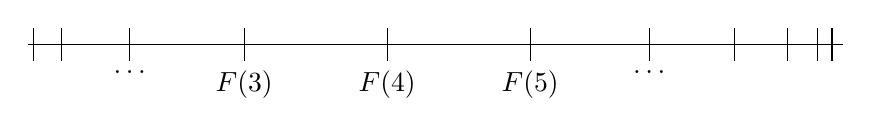
\begin{tikzpicture}[scale=0.03\textwidth]
	\draw (0,0) -- (1,0);
	\draw (0.0067, -0.02) -- (0.0067, 0.02);
	\draw (0.0404, -0.02) -- (0.0404, 0.02);
	\draw (0.1246, -0.02) node[below]{$\hdots$}
	-- (0.1246, 0.02);
	\draw (0.2650, -0.02) node[below]{$F(3)$}
	-- (0.2650, 0.02);
	\draw (0.4404, -0.02) node[below]{$F(4)$}
	-- (0.4404, 0.02);
	\draw (0.6159, -0.02) node[below]{$F(5)$}
	-- (0.6159, 0.02);
	\draw (0.7621, -0.02) node[below]{$\hdots$}
	-- (0.7621, 0.02);
	\draw (0.8666, -0.02) -- (0.8666, 0.02);
	\draw (0.9319, -0.02) -- (0.9319, 0.02);
	\draw (0.9681, -0.02) -- (0.9681, 0.02);
	\draw (0.9863, -0.02) -- (0.9863, 0.02);
	\end{tikzpicture}
	\caption{The unit interval divided into sections according to the Poisson distribution function when $\lambda = 5$}
	\label{fig:inverse}
\end{figure}

We can easily make this procedure exact by sampling the digits of $X$ one by one and computing the leading digits of $F$ for the various relevant values of $n$. Eventually we'll have $X$ completely fenced in between $F(n)$ and $F(n+1)$ for some $n$, at which point none of the remaining digits of any of the involved quantities matter, so we can return $n+1$.

\section{Exact Rejection Sampling}

At this point we'll turn our attention to continuous distributions. Immediately a problem presents itself here. That is a sample from a continuous distribution will typically be an irrational number with infinitely many digits in its decimal representation. How can we hope to draw an exact sample if just printing it out is an indeterminate process?\\
Clearly, we'll have to manage our expectations as to what we can accomplish here. But if all we ask for is a method that will produce arbitrarily many correct digits of an exact sample, then there are already plenty of methods available.

Take the well known inverse sampling method. In the case of the exponential distribution with $\lambda = 1$ this method amounts to simply computing $-\ln(1-X)$ where $X \sim \text{U}[0,1]$. This task can be performed to arbitrary precision. So in the sense just described exact sampling would be quite uninteresting.

But there's another sense in which exact sampling can be accomplished which isn't quite as trivial. We can try to sample just the leading digits of an exact sample so that the remaining digits then no longer depend on the distribution we're sampling from. In particular we'll see a way to sample leading digits, which we'll call a prefix, so that the remaining digits will be uniformly random. A prefix thus completely captures the characteristics of the distribution and so can arguably be referred to as an exact sample.

The tool we'll use to accomplish this is a modification of rejection sampling. Let's focus on the interval [0,1] and let's choose for the purpose of illustration the distribution with density $f(x) = 2x$ as our target. The method of rejection sampling goes back to John von Neumann and is usually stated in terms of some proposal distribution. But we'll focus on the case where the uniform distribution on $[0,1]$ is our proposal distribution, because that's what our infinite stream of random bits most readily supplies.

Rejection sampling then says to do the following:
\begin{enumerate}
    \item Draw a sample $x$ from the proposal distribution U$[0,1]$
    \item Accept $x$ as the sample with probability $\frac{2x}{2} = x$ (we'll do so by comparing $2x$ to another sample from U$[0,2]$)
    \item If $x$ was rejected, start over
\end{enumerate}
These steps can be visualized as in figure \ref{fig:rejection_0}. We draw a sample from the uniform distribution on the rectangle enclosing our target density function. If it falls below the density function, the x-coordinate of that point becomes the sample.

\begin{figure}
    \centering
    \begin{tikzpicture}[scale=1.3]
    \begin{axis}
    \addplot[mark=none,very thick,color=blue] coordinates {(0, 0) (1, 2)};
    \path[fill=gray!15] (0, 0) -- (100, 0) -- (100, 200) -- cycle;
    \node[circle,fill=red,scale=0.5] at (60, 70) {};
    \end{axis}
    \end{tikzpicture}
    \caption{Rejection Sampling --- Samples that fall in the shaded region (as shown) are accepted}
    \label{fig:rejection_0}
\end{figure}

There are plenty of expositions in the literature that give a more thorough justification of these steps. The way this is usually implemented is by approximating the uniform distribution using some finite number of bits, inevitably incurring some error. But using exact Bernoulli sampling we can do better.

In essence, we'll consider the rectangle defined by the leading digits of $x$ and $y$. By drawing additional digits for $x$ and $y$ we can shrink this rectangle arbitrarily small until we're certain that it falls either wholly below or above $f$. At that point we know whether to accept or reject, without having to examine further digits. Let's walk through an example.

Suppose the leading bits of our uniform sample $x$ for the x-coordinate are $101...\,.$ This narrows down our sample to the interval [0.625, 0.75]. We can think of this as defining a $\delta$-environment from basic calculus. This in turn defines a corresponding $\epsilon$-environment [1.25, 1.5] into which $2x$ falls.

Furthermore, let's imagine that the leading bits of our second sample $y$, drawn from U[0, 2], were $1001...\,.$ This allows us to narrow down $y$ to [1.125, 1.375]. Figure \ref{fig:rejection_1} shows what's going on.

\begin{figure}[h]
    \centering
    \begin{tikzpicture}[scale=1.3]
    \begin{axis}
    \path[fill=gray!15] (10, 137.5) -- (90, 137.5) -- (90, 150) -- (10, 150);
    
    \path[fill=gray!30] (20, 125) -- (90, 125) -- (90, 137.5) -- (20, 137.5);
    
    \path[fill=gray!15] (10, 125) -- (20, 125) -- (20, 137.5) -- (10, 137.5);
    
    \path[fill=gray!15] (90, 125) -- (100, 125) -- (100, 137.5) -- (90, 137.5);
    
    \path[fill=gray!15] (20, 112.5) -- (100, 112.5) -- (100, 125) -- (20, 125);
    
    \addplot[mark=none,very thick, color=blue] coordinates {(0, 0) (1, 2)};
    
    \draw[dashed] (62.5, 0) -- (62.5, 200);
    \draw[dashed] (75, 0) -- (75, 200);
    
    \draw[dashed] (10, 150) -- (90, 150);
    \draw[dashed] (10, 125) -- (90, 125);
    
    \draw[dashed] (20, 137.5) -- (100, 137.5);
    \draw[dashed] (20, 112.5) -- (100, 112.5);
    
    \draw[decoration={brace, mirror}, decorate] (101, 112.5) -- node[right] {$y$} (101, 137.5);
    
    \draw[decoration={brace}, decorate] (9, 125) -- node[left] {$f(x)$} (9, 150);
    
    \draw[decoration={brace, mirror}, decorate] (62.5, -1) -- node[below] {$x$} (75, -1);
    \end{axis}
    \end{tikzpicture}
    \caption{Having drawn $x = 0.101..._2$ and $y = 1.001..._2$ we know that $f(x)$ and $y$ fall somewhere into these intervals}
    \label{fig:rejection_1}
\end{figure}

Now these intervals for $f(x)$ and $y$ overlap. So we can't say for certain whether $x$ should be rejected or not. But that's easy to remedy. Just draw additional bits for $x$ and $y$. Sooner or later (and chances are sooner) these intervals will separate. And then we'll know whether to accept $x$ or to try again.

But note that something remarkable happens as soon as we accept $x$. At that point we've determined some of the leading bits of $x$ through careful testing with the rejection method. But the remaining bits can now be drawn from our infinite random bit supply without any further thought! We can forget all about the function $f(x)=2x$ and just pump out the remaining bits of our sample as fast as our random number generator is able to mint them.\\\noindent

The previous discussion was loosely inspired by work from C. Karney in \cite{Karney}. Though Karney only focuses on the normal distribution and its counterpart, the discrete normal distribution, and doesn't employ rejection sampling. Instead it uses a less general tailor made algorithm.

\section{Putting It All Together}

Now let's take these two previous ideas and put them together. How could we draw an exact sample from the standard normal distribution? At this point it's simple. First, use exact bisection sampling and perform a random walk on the integers, starting at 0. As soon as the sample has been narrowed down to an interval of unit length, the integer part of the sample has been determined. Then use exact rejection sampling to determine the fractional part. That's all there is to it. We can now easily produce the digits of an exactly standard normally distributed sample to our hearts content.\\

At this point it seems worth reflecting a little more generally. First, because we're eventually just passing through random bits, this algorithm can easily be seen to be asymptotically optimal. We'll examine the exact meaning of "eventually" in section 7. For now, let's direct our attention to the bits required to sample $x$ during the rejection sampling stage. A few of these bits will be discarded while we iterate the rejection method. But the rest is then returned completely unmodified. A different way of looking at this is that we're taking a sample from the uniform distribution and sawing off a little piece at the front. The tail end is then precisely the fractional part of a random variable having practically any desired continuous distribution.

Furthermore, we could have used the exact same sequence to also draw an exact sample from some other unrelated distribution. These two samples would then be correlated in the curious way that, at some offset, eventually all of their digits coincide. Stated differently, if one looks at a sample from the uniform distribution, chances are that, \textit{within eyesight}, one can see the superimposed beginnings of samples from any continuous distribution one can care to mention.

Finally, consider the following. After having determined the leading digits of a sample from some distribution, we could write them down on a slip of paper and pass it to somebody else. We'll call such string of digits a \textit{prefix}. That person wouldn't even have to know which distribution the prefix was drawn from. They would still hold in their hands an \textit{exact} sample. If they're unsatisfied with the precision of the prefix we gave them, they can just add their own random digits! In very much the same way that the symbol $\pi$ summarizes an infinite sequence of digits, so do the digits on that slip of paper.

As an aside, it is also possible, in a sense, to reconstitute a prefix once many random digits have already been attached. Though this may easily be a different prefix and one does now need the density $f$ of the distribution from which the sample is drawn. The idea is to simply perform rejection sampling using $f$ as a proposal density and the uniform as the target distribution. As soon as a uniform has been successfully drawn, one can be confident that the remaining, unexamined digits are uniform, thus the digits consumed so far constitute a prefix. One caveat here is that one has to condition and rescale $f$ every time a rejection takes place, because, unlike with the uniform distribution, the trailing digits of $f$ are unlikely to again be distributed according to $f$. While this would be a daunting challenge to program, considering one requires arbitrary precision, there is nothing that prevents this in principle.

Now it is tempting to refer to the distribution of numbers that we could write on that slip of paper as a \textit{prefix distribution}. There's just one slight wrinkle that we have to iron out before we're fully justified to make that designation. The problem is that distinct prefixes may denote the same real number. Take the prefixes $0$ and $00$. Both of these designate distinct prefixes. One cannot replace one with the other without altering the underlying distribution that one is sampling. But if forced to map these to real numbers one would end up on the same point on the number line.

The way out here is to realize that we're free to add some random bits of our own before passing along the slip of paper. So all we do is sample bits until we hit a $1$. At that point our prefix designates a unique real number and we terminate. In effect we've just done a little part of the other person's job. Let's refer to these elongated prefixes as \textit{padded prefixes} as opposed to \textit{unpadded prefixes} for their unmodified counterparts. If it is clear from context we'll also often just use the term \textit{prefix} for either version.

\section{Graphing Prefix Distributions}

It's usually best to begin building an intuition for something new by producing some visual aids. So what we'll start with is to find ways to graph prefix distributions. For this we'll have to find a way to compute the probabilities of various prefixes occurring. Perhaps surprisingly these probabilities can be represented in a quite natural visual form.

\subsection{Unpadded Prefix Probabilities}

Let's stick to the example of the normal distribution on the interval $[0,1]$. And let's momentarily focus only on unpadded prefixes. Then figure \ref{fig:normal_bin_cover} shows a graphical representation of the probabilities for various prefixes.

\begin{figure}
    \centering
    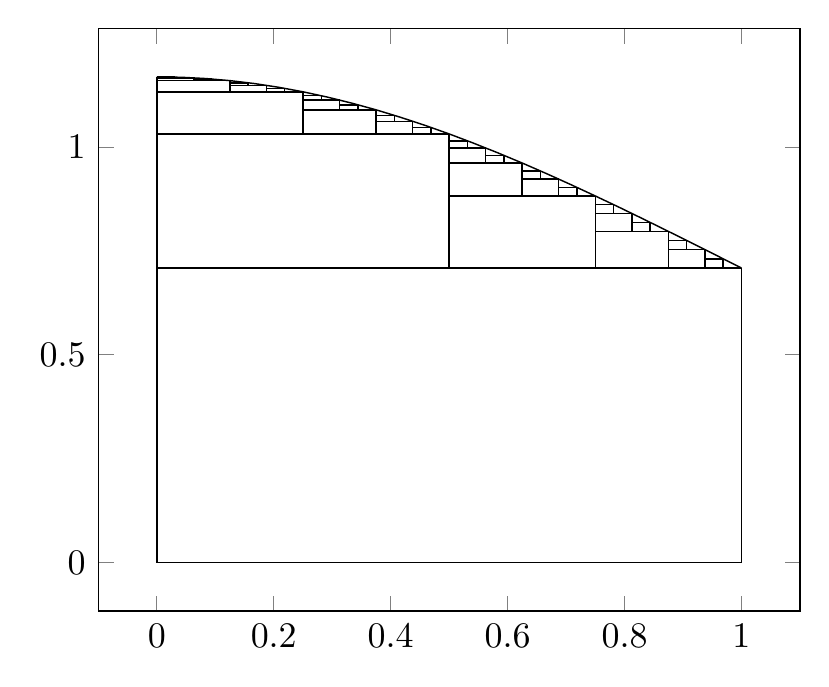
\begin{tikzpicture}[scale=1.3]
\begin{axis}
\addplot[draw=none] coordinates {(0,0)};
\addplot[domain=0:1] {e^(-x^2/2)/0.855624};
\draw (axis cs: 0, 0) -- (axis cs: 1, 0);
\draw (axis cs: 0, 0) -- (axis cs: 0, 0.7088752307384394);
\draw (axis cs: 1, 0) -- (axis cs: 1, 0.7088752307384394);
\draw (axis cs: 0, 0.7088752307384394) -- (axis cs: 1, 0.7088752307384394);
\draw (axis cs: 0, 0.7088752307384394) -- (axis cs: 0, 1.0314073738483691);
\draw (axis cs: 1/2, 0.7088752307384394) -- (axis cs: 1/2, 1.0314073738483691);
\draw (axis cs: 0, 1.0314073738483691) -- (axis cs: 1/2, 1.0314073738483691);
\draw (axis cs: 1/2, 0.7088752307384394) -- (axis cs: 1/2, 0.7088752311585824);
\draw (axis cs: 1, 0.7088752307384394) -- (axis cs: 1, 0.7088752311585824);
\draw (axis cs: 1/2, 0.7088752311585824) -- (axis cs: 1, 0.7088752311585824);
\draw (axis cs: 0, 1.0314073738483691) -- (axis cs: 0, 1.132779392052711);
\draw (axis cs: 1/4, 1.0314073738483691) -- (axis cs: 1/4, 1.132779392052711);
\draw (axis cs: 0, 1.132779392052711) -- (axis cs: 1/4, 1.132779392052711);
\draw (axis cs: 1/4, 1.0314073738483691) -- (axis cs: 1/4, 1.0314073740037737);
\draw (axis cs: 1/2, 1.0314073738483691) -- (axis cs: 1/2, 1.0314073740037737);
\draw (axis cs: 1/4, 1.0314073740037737) -- (axis cs: 1/2, 1.0314073740037737);
\draw (axis cs: 1/2, 0.7088752311585824) -- (axis cs: 1/2, 0.8822094784609293);
\draw (axis cs: 3/4, 0.7088752311585824) -- (axis cs: 3/4, 0.8822094784609293);
\draw (axis cs: 1/2, 0.8822094784609293) -- (axis cs: 3/4, 0.8822094784609293);
\draw (axis cs: 3/4, 0.7088752311585824) -- (axis cs: 3/4, 0.7088752308298532);
\draw (axis cs: 1, 0.7088752311585824) -- (axis cs: 1, 0.7088752308298532);
\draw (axis cs: 3/4, 0.7088752308298532) -- (axis cs: 1, 0.7088752308298532);
\draw (axis cs: 0, 1.132779392052711) -- (axis cs: 0, 1.1596424811335069);
\draw (axis cs: 1/8, 1.132779392052711) -- (axis cs: 1/8, 1.1596424811335069);
\draw (axis cs: 0, 1.1596424811335069) -- (axis cs: 1/8, 1.1596424811335069);
\draw (axis cs: 1/8, 1.132779392052711) -- (axis cs: 1/8, 1.1327793920967966);
\draw (axis cs: 1/4, 1.132779392052711) -- (axis cs: 1/4, 1.1327793920967966);
\draw (axis cs: 1/8, 1.1327793920967966) -- (axis cs: 1/4, 1.1327793920967966);
\draw (axis cs: 1/4, 1.0314073740037737) -- (axis cs: 1/4, 1.0893832952435563);
\draw (axis cs: 3/8, 1.0314073740037737) -- (axis cs: 3/8, 1.0893832952435563);
\draw (axis cs: 1/4, 1.0893832952435563) -- (axis cs: 3/8, 1.0893832952435563);
\draw (axis cs: 3/8, 1.0314073740037737) -- (axis cs: 3/8, 1.0314073738816207);
\draw (axis cs: 1/2, 1.0314073740037737) -- (axis cs: 1/2, 1.0314073738816207);
\draw (axis cs: 3/8, 1.0314073738816207) -- (axis cs: 1/2, 1.0314073738816207);
\draw (axis cs: 1/2, 0.8822094784609293) -- (axis cs: 1/2, 0.9613773842172454);
\draw (axis cs: 5/8, 0.8822094784609293) -- (axis cs: 5/8, 0.9613773842172454);
\draw (axis cs: 1/2, 0.9613773842172454) -- (axis cs: 5/8, 0.9613773842172454);
\draw (axis cs: 5/8, 0.8822094784609293) -- (axis cs: 5/8, 0.8822094782504817);
\draw (axis cs: 3/4, 0.8822094784609293) -- (axis cs: 3/4, 0.8822094782504817);
\draw (axis cs: 5/8, 0.8822094782504817) -- (axis cs: 3/4, 0.8822094782504817);
\draw (axis cs: 3/4, 0.7088752308298532) -- (axis cs: 3/4, 0.797009845188235);
\draw (axis cs: 7/8, 0.7088752308298532) -- (axis cs: 7/8, 0.797009845188235);
\draw (axis cs: 3/4, 0.797009845188235) -- (axis cs: 7/8, 0.797009845188235);
\draw (axis cs: 7/8, 0.7088752308298532) -- (axis cs: 7/8, 0.7088752312325376);
\draw (axis cs: 1, 0.7088752308298532) -- (axis cs: 1, 0.7088752312325376);
\draw (axis cs: 7/8, 0.7088752312325376) -- (axis cs: 1, 0.7088752312325376);
\draw (axis cs: 0, 1.1596424811335069) -- (axis cs: 0, 1.1664572068057864);
\draw (axis cs: 1/16, 1.1596424811335069) -- (axis cs: 1/16, 1.1664572068057864);
\draw (axis cs: 0, 1.1664572068057864) -- (axis cs: 1/16, 1.1664572068057864);
\draw (axis cs: 1/16, 1.1596424811335069) -- (axis cs: 1/16, 1.1596424811455144);
\draw (axis cs: 1/8, 1.1596424811335069) -- (axis cs: 1/8, 1.1596424811455144);
\draw (axis cs: 1/16, 1.1596424811455144) -- (axis cs: 1/8, 1.1596424811455144);
\draw (axis cs: 1/8, 1.1327793920967966) -- (axis cs: 1/8, 1.1483729640867604);
\draw (axis cs: 3/16, 1.1327793920967966) -- (axis cs: 3/16, 1.1483729640867604);
\draw (axis cs: 1/8, 1.1483729640867604) -- (axis cs: 3/16, 1.1483729640867604);
\draw (axis cs: 3/16, 1.1327793920967966) -- (axis cs: 3/16, 1.132779392061841);
\draw (axis cs: 1/4, 1.1327793920967966) -- (axis cs: 1/4, 1.132779392061841);
\draw (axis cs: 3/16, 1.132779392061841) -- (axis cs: 1/4, 1.132779392061841);
\draw (axis cs: 1/4, 1.0893832952435563) -- (axis cs: 1/4, 1.1130412424936);
\draw (axis cs: 5/16, 1.0893832952435563) -- (axis cs: 5/16, 1.1130412424936);
\draw (axis cs: 1/4, 1.1130412424936) -- (axis cs: 5/16, 1.1130412424936);
\draw (axis cs: 5/16, 1.0893832952435563) -- (axis cs: 5/16, 1.0893832951765468);
\draw (axis cs: 3/8, 1.0893832952435563) -- (axis cs: 3/8, 1.0893832951765468);
\draw (axis cs: 5/16, 1.0893832951765468) -- (axis cs: 3/8, 1.0893832951765468);
\draw (axis cs: 3/8, 1.0314073738816207) -- (axis cs: 3/8, 1.0620713731210203);
\draw (axis cs: 7/16, 1.0314073738816207) -- (axis cs: 7/16, 1.0620713731210203);
\draw (axis cs: 3/8, 1.0620713731210203) -- (axis cs: 7/16, 1.0620713731210203);
\draw (axis cs: 7/16, 1.0314073738816207) -- (axis cs: 7/16, 1.0314073740306748);
\draw (axis cs: 1/2, 1.0314073738816207) -- (axis cs: 1/2, 1.0314073740306748);
\draw (axis cs: 7/16, 1.0314073740306748) -- (axis cs: 1/2, 1.0314073740306748);
\draw (axis cs: 1/2, 0.9613773842172454) -- (axis cs: 1/2, 0.9977237218622059);
\draw (axis cs: 9/16, 0.9613773842172454) -- (axis cs: 9/16, 0.9977237218622059);
\draw (axis cs: 1/2, 0.9977237218622059) -- (axis cs: 9/16, 0.9977237218622059);
\draw (axis cs: 9/16, 0.9613773842172454) -- (axis cs: 9/16, 0.961377384050528);
\draw (axis cs: 5/8, 0.9613773842172454) -- (axis cs: 5/8, 0.961377384050528);
\draw (axis cs: 9/16, 0.961377384050528) -- (axis cs: 5/8, 0.961377384050528);
\draw (axis cs: 5/8, 0.8822094782504817) -- (axis cs: 5/8, 0.9227436001143932);
\draw (axis cs: 11/16, 0.8822094782504817) -- (axis cs: 11/16, 0.9227436001143932);
\draw (axis cs: 5/8, 0.9227436001143932) -- (axis cs: 11/16, 0.9227436001143932);
\draw (axis cs: 11/16, 0.8822094782504817) -- (axis cs: 11/16, 0.882209478516775);
\draw (axis cs: 3/4, 0.8822094782504817) -- (axis cs: 3/4, 0.882209478516775);
\draw (axis cs: 11/16, 0.882209478516775) -- (axis cs: 3/4, 0.882209478516775);
\draw (axis cs: 3/4, 0.797009845188235) -- (axis cs: 3/4, 0.8401676093632154);
\draw (axis cs: 13/16, 0.797009845188235) -- (axis cs: 13/16, 0.8401676093632154);
\draw (axis cs: 3/4, 0.8401676093632154) -- (axis cs: 13/16, 0.8401676093632154);
\draw (axis cs: 13/16, 0.797009845188235) -- (axis cs: 13/16, 0.7970098455560798);
\draw (axis cs: 7/8, 0.797009845188235) -- (axis cs: 7/8, 0.7970098455560798);
\draw (axis cs: 13/16, 0.7970098455560798) -- (axis cs: 7/8, 0.7970098455560798);
\draw (axis cs: 7/8, 0.7088752312325376) -- (axis cs: 7/8, 0.7531213777701796);
\draw (axis cs: 15/16, 0.7088752312325376) -- (axis cs: 15/16, 0.7531213777701796);
\draw (axis cs: 7/8, 0.7531213777701796) -- (axis cs: 15/16, 0.7531213777701796);
\draw (axis cs: 15/16, 0.7088752312325376) -- (axis cs: 15/16, 0.7088752309266617);
\draw (axis cs: 1, 0.7088752312325376) -- (axis cs: 1, 0.7088752309266617);
\draw (axis cs: 15/16, 0.7088752309266617) -- (axis cs: 1, 0.7088752309266617);
\draw (axis cs: 0, 1.1664572068057864) -- (axis cs: 0, 1.168167136431449);
\draw (axis cs: 1/32, 1.1664572068057864) -- (axis cs: 1/32, 1.168167136431449);
\draw (axis cs: 0, 1.168167136431449) -- (axis cs: 1/32, 1.168167136431449);
\draw (axis cs: 1/32, 1.1664572068057864) -- (axis cs: 1/32, 1.1664572068035775);
\draw (axis cs: 1/16, 1.1664572068057864) -- (axis cs: 1/16, 1.1664572068035775);
\draw (axis cs: 1/32, 1.1664572068035775) -- (axis cs: 1/16, 1.1664572068035775);
\draw (axis cs: 1/16, 1.1596424811455144) -- (axis cs: 1/16, 1.1636128843863704);
\draw (axis cs: 3/32, 1.1596424811455144) -- (axis cs: 3/32, 1.1636128843863704);
\draw (axis cs: 1/16, 1.1636128843863704) -- (axis cs: 3/32, 1.1636128843863704);
\draw (axis cs: 3/32, 1.1596424811455144) -- (axis cs: 3/32, 1.1596424811358435);
\draw (axis cs: 1/8, 1.1596424811455144) -- (axis cs: 1/8, 1.1596424811358435);
\draw (axis cs: 3/32, 1.1596424811358435) -- (axis cs: 1/8, 1.1596424811358435);
\draw (axis cs: 1/8, 1.1483729640867604) -- (axis cs: 1/8, 1.154557577111731);
\draw (axis cs: 5/32, 1.1483729640867604) -- (axis cs: 5/32, 1.154557577111731);
\draw (axis cs: 1/8, 1.154557577111731) -- (axis cs: 5/32, 1.154557577111731);
\draw (axis cs: 5/32, 1.1483729640867604) -- (axis cs: 5/32, 1.1483729640680242);
\draw (axis cs: 3/16, 1.1483729640867604) -- (axis cs: 3/16, 1.1483729640680242);
\draw (axis cs: 5/32, 1.1483729640680242) -- (axis cs: 3/16, 1.1483729640680242);
\draw (axis cs: 3/16, 1.132779392061841) -- (axis cs: 3/16, 1.141106573919148);
\draw (axis cs: 7/32, 1.132779392061841) -- (axis cs: 7/32, 1.141106573919148);
\draw (axis cs: 3/16, 1.141106573919148) -- (axis cs: 7/32, 1.141106573919148);
\draw (axis cs: 7/32, 1.132779392061841) -- (axis cs: 7/32, 1.1327793921041829);
\draw (axis cs: 1/4, 1.132779392061841) -- (axis cs: 1/4, 1.1327793921041829);
\draw (axis cs: 7/32, 1.1327793921041829) -- (axis cs: 1/4, 1.1327793921041829);
\draw (axis cs: 1/4, 1.1130412424936) -- (axis cs: 1/4, 1.1234153563552949);
\draw (axis cs: 9/32, 1.1130412424936) -- (axis cs: 9/32, 1.1234153563552949);
\draw (axis cs: 1/4, 1.1234153563552949) -- (axis cs: 9/32, 1.1234153563552949);
\draw (axis cs: 9/32, 1.1130412424936) -- (axis cs: 9/32, 1.1130412424436062);
\draw (axis cs: 5/16, 1.1130412424936) -- (axis cs: 5/16, 1.1130412424436062);
\draw (axis cs: 9/32, 1.1130412424436062) -- (axis cs: 5/16, 1.1130412424436062);
\draw (axis cs: 5/16, 1.0893832951765468) -- (axis cs: 5/16, 1.1016865364282735);
\draw (axis cs: 11/32, 1.0893832951765468) -- (axis cs: 11/32, 1.1016865364282735);
\draw (axis cs: 5/16, 1.1016865364282735) -- (axis cs: 11/32, 1.1016865364282735);
\draw (axis cs: 11/32, 1.0893832951765468) -- (axis cs: 11/32, 1.0893832952607965);
\draw (axis cs: 3/8, 1.0893832951765468) -- (axis cs: 3/8, 1.0893832952607965);
\draw (axis cs: 11/32, 1.0893832952607965) -- (axis cs: 3/8, 1.0893832952607965);
\draw (axis cs: 3/8, 1.0620713731210203) -- (axis cs: 3/8, 1.0761659954808578);
\draw (axis cs: 13/32, 1.0620713731210203) -- (axis cs: 13/32, 1.0761659954808578);
\draw (axis cs: 3/8, 1.0761659954808578) -- (axis cs: 13/32, 1.0761659954808578);
\draw (axis cs: 13/32, 1.0620713731210203) -- (axis cs: 13/32, 1.0620713732458882);
\draw (axis cs: 7/16, 1.0620713731210203) -- (axis cs: 7/16, 1.0620713732458882);
\draw (axis cs: 13/32, 1.0620713732458882) -- (axis cs: 7/16, 1.0620713732458882);
\draw (axis cs: 7/16, 1.0314073740306748) -- (axis cs: 7/16, 1.047138253842928);
\draw (axis cs: 15/32, 1.0314073740306748) -- (axis cs: 15/32, 1.047138253842928);
\draw (axis cs: 7/16, 1.047138253842928) -- (axis cs: 15/32, 1.047138253842928);
\draw (axis cs: 15/32, 1.0314073740306748) -- (axis cs: 15/32, 1.0314073739168346);
\draw (axis cs: 1/2, 1.0314073740306748) -- (axis cs: 1/2, 1.0314073739168346);
\draw (axis cs: 15/32, 1.0314073739168346) -- (axis cs: 1/2, 1.0314073739168346);
\draw (axis cs: 1/2, 0.9977237218622059) -- (axis cs: 1/2, 1.0149211967297487);
\draw (axis cs: 17/32, 0.9977237218622059) -- (axis cs: 17/32, 1.0149211967297487);
\draw (axis cs: 1/2, 1.0149211967297487) -- (axis cs: 17/32, 1.0149211967297487);
\draw (axis cs: 17/32, 0.9977237218622059) -- (axis cs: 17/32, 0.9977237217032419);
\draw (axis cs: 9/16, 0.9977237218622059) -- (axis cs: 9/16, 0.9977237217032419);
\draw (axis cs: 17/32, 0.9977237217032419) -- (axis cs: 9/16, 0.9977237217032419);
\draw (axis cs: 9/16, 0.961377384050528) -- (axis cs: 9/16, 0.9798602895103428);
\draw (axis cs: 19/32, 0.961377384050528) -- (axis cs: 19/32, 0.9798602895103428);
\draw (axis cs: 9/16, 0.9798602895103428) -- (axis cs: 19/32, 0.9798602895103428);
\draw (axis cs: 19/32, 0.961377384050528) -- (axis cs: 19/32, 0.961377384258274);
\draw (axis cs: 5/8, 0.961377384050528) -- (axis cs: 5/8, 0.961377384258274);
\draw (axis cs: 19/32, 0.961377384258274) -- (axis cs: 5/8, 0.961377384258274);
\draw (axis cs: 5/8, 0.9227436001143932) -- (axis cs: 5/8, 0.9423224317184322);
\draw (axis cs: 21/32, 0.9227436001143932) -- (axis cs: 21/32, 0.9423224317184322);
\draw (axis cs: 5/8, 0.9423224317184322) -- (axis cs: 21/32, 0.9423224317184322);
\draw (axis cs: 21/32, 0.9227436001143932) -- (axis cs: 21/32, 0.9227436003733795);
\draw (axis cs: 11/16, 0.9227436001143932) -- (axis cs: 11/16, 0.9227436003733795);
\draw (axis cs: 21/32, 0.9227436003733795) -- (axis cs: 11/16, 0.9227436003733795);
\draw (axis cs: 11/16, 0.882209478516775) -- (axis cs: 11/16, 0.9026895991370857);
\draw (axis cs: 23/32, 0.882209478516775) -- (axis cs: 23/32, 0.9026895991370857);
\draw (axis cs: 11/16, 0.9026895991370857) -- (axis cs: 23/32, 0.9026895991370857);
\draw (axis cs: 23/32, 0.882209478516775) -- (axis cs: 23/32, 0.8822094783235847);
\draw (axis cs: 3/4, 0.882209478516775) -- (axis cs: 3/4, 0.8822094783235847);
\draw (axis cs: 23/32, 0.8822094783235847) -- (axis cs: 3/4, 0.8822094783235847);
\draw (axis cs: 3/4, 0.8401676093632154) -- (axis cs: 3/4, 0.8613524328407608);
\draw (axis cs: 25/32, 0.8401676093632154) -- (axis cs: 25/32, 0.8613524328407608);
\draw (axis cs: 3/4, 0.8613524328407608) -- (axis cs: 25/32, 0.8613524328407608);
\draw (axis cs: 25/32, 0.8401676093632154) -- (axis cs: 25/32, 0.840167609121235);
\draw (axis cs: 13/16, 0.8401676093632154) -- (axis cs: 13/16, 0.840167609121235);
\draw (axis cs: 25/32, 0.840167609121235) -- (axis cs: 13/16, 0.840167609121235);
\draw (axis cs: 13/16, 0.7970098455560798) -- (axis cs: 13/16, 0.8187039166526356);
\draw (axis cs: 27/32, 0.7970098455560798) -- (axis cs: 27/32, 0.8187039166526356);
\draw (axis cs: 13/16, 0.8187039166526356) -- (axis cs: 27/32, 0.8187039166526356);
\draw (axis cs: 27/32, 0.7970098455560798) -- (axis cs: 27/32, 0.7970098452652852);
\draw (axis cs: 7/8, 0.7970098455560798) -- (axis cs: 7/8, 0.7970098452652852);
\draw (axis cs: 27/32, 0.7970098452652852) -- (axis cs: 7/8, 0.7970098452652852);
\draw (axis cs: 7/8, 0.7531213777701796) -- (axis cs: 7/8, 0.7751332890022959);
\draw (axis cs: 29/32, 0.7531213777701796) -- (axis cs: 29/32, 0.7751332890022959);
\draw (axis cs: 7/8, 0.7751332890022959) -- (axis cs: 29/32, 0.7751332890022959);
\draw (axis cs: 29/32, 0.7531213777701796) -- (axis cs: 29/32, 0.7531213774397331);
\draw (axis cs: 15/16, 0.7531213777701796) -- (axis cs: 15/16, 0.7531213774397331);
\draw (axis cs: 29/32, 0.7531213774397331) -- (axis cs: 15/16, 0.7531213774397331);
\draw (axis cs: 15/16, 0.7088752309266617) -- (axis cs: 15/16, 0.7310203152337048);
\draw (axis cs: 31/32, 0.7088752309266617) -- (axis cs: 31/32, 0.7310203152337048);
\draw (axis cs: 15/16, 0.7310203152337048) -- (axis cs: 31/32, 0.7310203152337048);
\draw (axis cs: 31/32, 0.7088752309266617) -- (axis cs: 31/32, 0.7088752313108574);
\draw (axis cs: 1, 0.7088752309266617) -- (axis cs: 1, 0.7088752313108574);
\draw (axis cs: 31/32, 0.7088752313108574) -- (axis cs: 1, 0.7088752313108574);
\end{axis}
\end{tikzpicture}
    \caption{The normal distribution on the interval $[0,1]$ divided up according to which sections produce distinct prefixes (prefixes up to length 6 have been plotted)}
    \label{fig:normal_bin_cover}
\end{figure}

For the following discussion it will be useful to think of our algorithm for exact rejection sampling as being very generous when sampling digits of $y$, whereas it only samples the absolute minimum required amount of digits for $x$. And recall that when performing rejection sampling we're eventually placing a uniformly random point on the area below the graph and then using the $x$-coordinate as our sample.\\
The large box at the bottom of figure \ref{fig:normal_bin_cover} covers all the positions for which we return the empty prefix. It cuts off at the top just at the value 0.709 which is the minimum of the normal distribution on the interval $[0,1]$ when conditioned on that interval. The reason this box corresponds to the empty prefix is that if we begin drawing samples for the $y$-coordinate of our uniform sample in $[0,1]\times[0,1.169]$ and we find that $y$ falls below this line, then we can already conclude that we're going to accept the $x$-coordinate as our normal sample, regardless of where it falls. So we don't even need to draw a single digit for $x$. On the other hand, if $y$ falls above 0.709, then we need further information about $x$ in order to decide whether to accept $x$ or discard it and try again. Since this requires sampling at least a single bit of $x$, the area above 0.709 corresponds entirely to other prefixes.

Let's discuss one more example. The second largest box in figure \ref{fig:normal_bin_cover}, situated in the top left, corresponds to the prefix 0. Here $y$ fell above 0.709, so we had to sample the first digit of $x$. This turned out to be 0, narrowing down our search to the left half. We then sampled $y$ to sufficient accuracy to determine that it fell below 1.031, the value at the midpoint of our distribution function. At that point we're again guaranteed to accept $x$ no matter its further digits. In a similar fashion we can cover the entire area with smaller and smaller rectangles.

Thus, the general method for finding the rectangle corresponding to a given prefix $p$ and density function $f$ is:
\begin{itemize}
    \item The left boundary is given by attaching infinitely many zeros, or equivalently by mapping $p$ to the directly corresponding real number.
    \item The right boundary is given by attaching infinitely many ones, or equivalently adding $2^{-n}$ if $p$ is of length $n$.
    \item The bottom boundary is given by removing the last digit of $p$ and finding the upper boundary of that prefix.
    \item The upper boundary is given by finding the minimum of $f$ over the interval delineated by the left and right boundaries.
\end{itemize}
Any sample from $\mathbb{R}^2$ that falls to the left or right of these boundaries will have an $x$-coordinate that disagrees with $p$. Any sample that falls within the interval, but below the lower boundary, will have been accepted before sampling all of $p$. And any sample that falls within the interval, but above the upper boundary, will require more information about the digits of the $x$-coordinate than $p$ can provide.

Conversely, any sample from $\mathbb{R}^2$ that falls within these boundaries corresponds to $p$, because, by the same arguments as in the previous paragraph, it doesn't correspond to any other prefix.

Furthermore, because we're picking the sample uniformly in the area below $f$ and because the total area below $f$ is exactly 1, the area of each of these rectangles is exactly equal to the probability that we'll pick the corresponding prefix.

This gives us not only a simple visualization of the probabilities involved, but also the means to compute these probabilities. In the following we use $\#p$ to denote the number of digits of $p$. $p_{-k}$ denotes $p$ with $k$ digits removed at the end. And $[p]$ is shorthand for the interval prefixed by $p$ - that is $[p] \coloneqq [p, p+2^{-\#p}]$ where the right-hand side is abusing notation slightly to use $p$ as a real number, not just as a string of bits. Then for a given unpadded prefix $p$ its probability to be picked is
\[
P_{\text{up}}(p) \coloneqq \underbrace{2^{-\#p}}_{\text{width of rectangle}}\:\cdot \underbrace{(\min_{[p_{-1}]} f - \min_{[p]} f)}_{\text{height of rectangle}}\,.
\]

(The up in $P_{\text{up}}$ stands for unpadded.) The only nontrivial hurdle that needs to be taken is to find means to minimize the given distribution function $f$ on arbitrary intervals. Though all the distribution functions we'll examine here will be so well behaved that this will be of no real practical concern.

\subsection{Padded Prefix Probabilities}

Now that we've seen how to determine the probabilities of unpadded prefixes we're ready to tackle the probabilities of padded prefixes. The only difference between these was that if a unpadded prefix didn't terminate with a 1, we would attach uniformly random bits until we hit a 1, giving us a padded prefix.

Let's interpret what this means in terms of figure \ref{fig:normal_bin_cover}. Take again the large box at the bottom corresponding to the empty prefix. This prefix doesn't end with a 1 (a special case which doesn't end with a 0 either), so it'll have to be padded. Half of the padded prefixes will have a 0 as their first bit, the other half a 1. We can visualize this by splitting the area corresponding to the empty prefix down the middle and erasing the top boundary. Doing this we're in effect "adding" half the probability of the empty prefix to the prefix 0 and half to the prefix 1.

The prefix 1 ends with a 1, so we're done there. This is not so with the prefix 0. It will have to be split again and have its upper boundary erased. The same will have to be done with the prefix 00, 000, etc. but also the prefix 10, 1010 and any other prefix ending with a 0. Performing this splitting and merging recursively for figure \ref{fig:normal_bin_cover} ultimately produces what can be seen in figure \ref{fig:normal_bin_cover_padded}.

\begin{figure}[h]
    \centering
    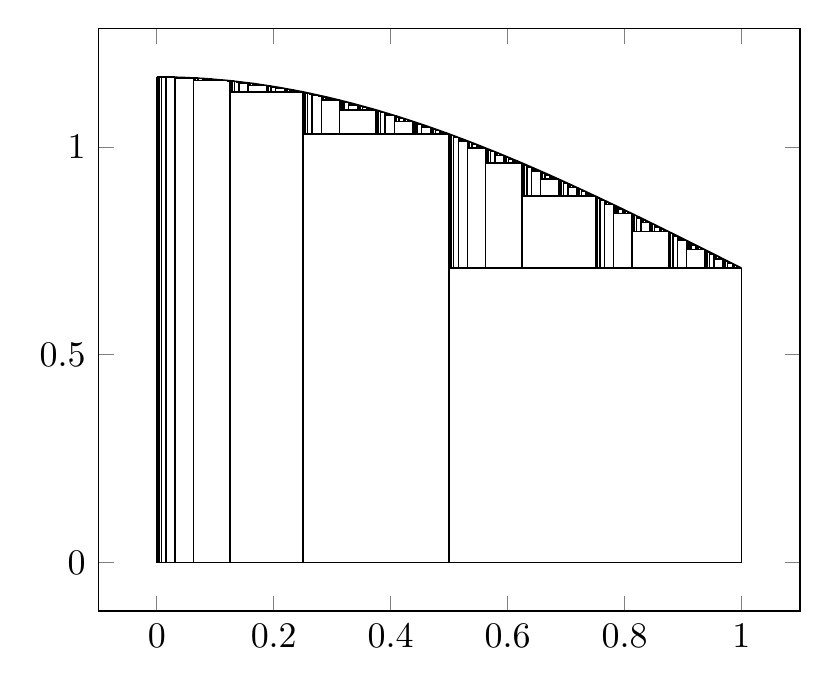
\begin{tikzpicture}[scale=1.3]
\begin{axis}
\addplot[draw=none] coordinates {(0,0)};
\addplot[domain=0:1] {e^(-x^2/2)/0.855624};
\draw (axis cs: 0, 0) -- (axis cs: 1, 0);
\draw (axis cs: 0, 0) -- (axis cs: 0, 0.7088752307384394);
\draw (axis cs: 1, 0) -- (axis cs: 1, 0.7088752307384394);
\draw (axis cs: 0, 0) -- (axis cs: 0, 1.0314073738483691);
\draw (axis cs: 1/2, 0) -- (axis cs: 1/2, 1.0314073738483691);
\draw (axis cs: 1/2, 0) -- (axis cs: 1/2, 0.7088752311585824);
\draw (axis cs: 1, 0) -- (axis cs: 1, 0.7088752311585824);
\draw (axis cs: 1/2, 0.7088752311585824) -- (axis cs: 1, 0.7088752311585824);
\draw (axis cs: 0, 0) -- (axis cs: 0, 1.132779392052711);
\draw (axis cs: 1/4, 0) -- (axis cs: 1/4, 1.132779392052711);
\draw (axis cs: 1/4, 0) -- (axis cs: 1/4, 1.0314073740037737);
\draw (axis cs: 1/2, 0) -- (axis cs: 1/2, 1.0314073740037737);
\draw (axis cs: 1/4, 1.0314073740037737) -- (axis cs: 1/2, 1.0314073740037737);
\draw (axis cs: 1/2, 0.7088752311585824) -- (axis cs: 1/2, 0.8822094784609293);
\draw (axis cs: 3/4, 0.7088752311585824) -- (axis cs: 3/4, 0.8822094784609293);
\draw (axis cs: 3/4, 0.7088752311585824) -- (axis cs: 3/4, 0.7088752308298532);
\draw (axis cs: 1, 0.7088752311585824) -- (axis cs: 1, 0.7088752308298532);
\draw (axis cs: 3/4, 0.7088752308298532) -- (axis cs: 1, 0.7088752308298532);
\draw (axis cs: 0, 0) -- (axis cs: 0, 1.1596424811335069);
\draw (axis cs: 1/8, 0) -- (axis cs: 1/8, 1.1596424811335069);
\draw (axis cs: 1/8, 0) -- (axis cs: 1/8, 1.1327793920967966);
\draw (axis cs: 1/4, 0) -- (axis cs: 1/4, 1.1327793920967966);
\draw (axis cs: 1/8, 1.1327793920967966) -- (axis cs: 1/4, 1.1327793920967966);
\draw (axis cs: 1/4, 1.0314073740037737) -- (axis cs: 1/4, 1.0893832952435563);
\draw (axis cs: 3/8, 1.0314073740037737) -- (axis cs: 3/8, 1.0893832952435563);
\draw (axis cs: 3/8, 1.0314073740037737) -- (axis cs: 3/8, 1.0314073738816207);
\draw (axis cs: 1/2, 1.0314073740037737) -- (axis cs: 1/2, 1.0314073738816207);
\draw (axis cs: 3/8, 1.0314073738816207) -- (axis cs: 1/2, 1.0314073738816207);
\draw (axis cs: 1/2, 0.7088752311585824) -- (axis cs: 1/2, 0.9613773842172454);
\draw (axis cs: 5/8, 0.7088752311585824) -- (axis cs: 5/8, 0.9613773842172454);
\draw (axis cs: 5/8, 0.7088752311585824) -- (axis cs: 5/8, 0.8822094782504817);
\draw (axis cs: 3/4, 0.7088752311585824) -- (axis cs: 3/4, 0.8822094782504817);
\draw (axis cs: 5/8, 0.8822094782504817) -- (axis cs: 3/4, 0.8822094782504817);
\draw (axis cs: 3/4, 0.7088752308298532) -- (axis cs: 3/4, 0.797009845188235);
\draw (axis cs: 7/8, 0.7088752308298532) -- (axis cs: 7/8, 0.797009845188235);
\draw (axis cs: 7/8, 0.7088752308298532) -- (axis cs: 7/8, 0.7088752312325376);
\draw (axis cs: 1, 0.7088752308298532) -- (axis cs: 1, 0.7088752312325376);
\draw (axis cs: 7/8, 0.7088752312325376) -- (axis cs: 1, 0.7088752312325376);
\draw (axis cs: 0, 0) -- (axis cs: 0, 1.1664572068057864);
\draw (axis cs: 1/16, 0) -- (axis cs: 1/16, 1.1664572068057864);
\draw (axis cs: 1/16, 0) -- (axis cs: 1/16, 1.1596424811455144);
\draw (axis cs: 1/8, 0) -- (axis cs: 1/8, 1.1596424811455144);
\draw (axis cs: 1/16, 1.1596424811455144) -- (axis cs: 1/8, 1.1596424811455144);
\draw (axis cs: 1/8, 1.1327793920967966) -- (axis cs: 1/8, 1.1483729640867604);
\draw (axis cs: 3/16, 1.1327793920967966) -- (axis cs: 3/16, 1.1483729640867604);
\draw (axis cs: 3/16, 1.1327793920967966) -- (axis cs: 3/16, 1.132779392061841);
\draw (axis cs: 1/4, 1.1327793920967966) -- (axis cs: 1/4, 1.132779392061841);
\draw (axis cs: 3/16, 1.132779392061841) -- (axis cs: 1/4, 1.132779392061841);
\draw (axis cs: 1/4, 1.0314073740037737) -- (axis cs: 1/4, 1.1130412424936);
\draw (axis cs: 5/16, 1.0314073740037737) -- (axis cs: 5/16, 1.1130412424936);
\draw (axis cs: 5/16, 1.0314073740037737) -- (axis cs: 5/16, 1.0893832951765468);
\draw (axis cs: 3/8, 1.0314073740037737) -- (axis cs: 3/8, 1.0893832951765468);
\draw (axis cs: 5/16, 1.0893832951765468) -- (axis cs: 3/8, 1.0893832951765468);
\draw (axis cs: 3/8, 1.0314073738816207) -- (axis cs: 3/8, 1.0620713731210203);
\draw (axis cs: 7/16, 1.0314073738816207) -- (axis cs: 7/16, 1.0620713731210203);
\draw (axis cs: 7/16, 1.0314073738816207) -- (axis cs: 7/16, 1.0314073740306748);
\draw (axis cs: 1/2, 1.0314073738816207) -- (axis cs: 1/2, 1.0314073740306748);
\draw (axis cs: 7/16, 1.0314073740306748) -- (axis cs: 1/2, 1.0314073740306748);
\draw (axis cs: 1/2, 0.7088752311585824) -- (axis cs: 1/2, 0.9977237218622059);
\draw (axis cs: 9/16, 0.7088752311585824) -- (axis cs: 9/16, 0.9977237218622059);
\draw (axis cs: 9/16, 0.7088752311585824) -- (axis cs: 9/16, 0.961377384050528);
\draw (axis cs: 5/8, 0.7088752311585824) -- (axis cs: 5/8, 0.961377384050528);
\draw (axis cs: 9/16, 0.961377384050528) -- (axis cs: 5/8, 0.961377384050528);
\draw (axis cs: 5/8, 0.8822094782504817) -- (axis cs: 5/8, 0.9227436001143932);
\draw (axis cs: 11/16, 0.8822094782504817) -- (axis cs: 11/16, 0.9227436001143932);
\draw (axis cs: 11/16, 0.8822094782504817) -- (axis cs: 11/16, 0.882209478516775);
\draw (axis cs: 3/4, 0.8822094782504817) -- (axis cs: 3/4, 0.882209478516775);
\draw (axis cs: 11/16, 0.882209478516775) -- (axis cs: 3/4, 0.882209478516775);
\draw (axis cs: 3/4, 0.7088752308298532) -- (axis cs: 3/4, 0.8401676093632154);
\draw (axis cs: 13/16, 0.7088752308298532) -- (axis cs: 13/16, 0.8401676093632154);
\draw (axis cs: 13/16, 0.7088752308298532) -- (axis cs: 13/16, 0.7970098455560798);
\draw (axis cs: 7/8, 0.7088752308298532) -- (axis cs: 7/8, 0.7970098455560798);
\draw (axis cs: 13/16, 0.7970098455560798) -- (axis cs: 7/8, 0.7970098455560798);
\draw (axis cs: 7/8, 0.7088752312325376) -- (axis cs: 7/8, 0.7531213777701796);
\draw (axis cs: 15/16, 0.7088752312325376) -- (axis cs: 15/16, 0.7531213777701796);
\draw (axis cs: 15/16, 0.7088752312325376) -- (axis cs: 15/16, 0.7088752309266617);
\draw (axis cs: 1, 0.7088752312325376) -- (axis cs: 1, 0.7088752309266617);
\draw (axis cs: 15/16, 0.7088752309266617) -- (axis cs: 1, 0.7088752309266617);
\draw (axis cs: 0, 0) -- (axis cs: 0, 1.168167136431449);
\draw (axis cs: 1/32, 0) -- (axis cs: 1/32, 1.168167136431449);
\draw (axis cs: 1/32, 0) -- (axis cs: 1/32, 1.1664572068035775);
\draw (axis cs: 1/16, 0) -- (axis cs: 1/16, 1.1664572068035775);
\draw (axis cs: 1/32, 1.1664572068035775) -- (axis cs: 1/16, 1.1664572068035775);
\draw (axis cs: 1/16, 1.1596424811455144) -- (axis cs: 1/16, 1.1636128843863704);
\draw (axis cs: 3/32, 1.1596424811455144) -- (axis cs: 3/32, 1.1636128843863704);
\draw (axis cs: 3/32, 1.1596424811455144) -- (axis cs: 3/32, 1.1596424811358435);
\draw (axis cs: 1/8, 1.1596424811455144) -- (axis cs: 1/8, 1.1596424811358435);
\draw (axis cs: 3/32, 1.1596424811358435) -- (axis cs: 1/8, 1.1596424811358435);
\draw (axis cs: 1/8, 1.1327793920967966) -- (axis cs: 1/8, 1.154557577111731);
\draw (axis cs: 5/32, 1.1327793920967966) -- (axis cs: 5/32, 1.154557577111731);
\draw (axis cs: 5/32, 1.1327793920967966) -- (axis cs: 5/32, 1.1483729640680242);
\draw (axis cs: 3/16, 1.1327793920967966) -- (axis cs: 3/16, 1.1483729640680242);
\draw (axis cs: 5/32, 1.1483729640680242) -- (axis cs: 3/16, 1.1483729640680242);
\draw (axis cs: 3/16, 1.132779392061841) -- (axis cs: 3/16, 1.141106573919148);
\draw (axis cs: 7/32, 1.132779392061841) -- (axis cs: 7/32, 1.141106573919148);
\draw (axis cs: 7/32, 1.132779392061841) -- (axis cs: 7/32, 1.1327793921041829);
\draw (axis cs: 1/4, 1.132779392061841) -- (axis cs: 1/4, 1.1327793921041829);
\draw (axis cs: 7/32, 1.1327793921041829) -- (axis cs: 1/4, 1.1327793921041829);
\draw (axis cs: 1/4, 1.0314073740037737) -- (axis cs: 1/4, 1.1234153563552949);
\draw (axis cs: 9/32, 1.0314073740037737) -- (axis cs: 9/32, 1.1234153563552949);
\draw (axis cs: 9/32, 1.0314073740037737) -- (axis cs: 9/32, 1.1130412424436062);
\draw (axis cs: 5/16, 1.0314073740037737) -- (axis cs: 5/16, 1.1130412424436062);
\draw (axis cs: 9/32, 1.1130412424436062) -- (axis cs: 5/16, 1.1130412424436062);
\draw (axis cs: 5/16, 1.0893832951765468) -- (axis cs: 5/16, 1.1016865364282735);
\draw (axis cs: 11/32, 1.0893832951765468) -- (axis cs: 11/32, 1.1016865364282735);
\draw (axis cs: 11/32, 1.0893832951765468) -- (axis cs: 11/32, 1.0893832952607965);
\draw (axis cs: 3/8, 1.0893832951765468) -- (axis cs: 3/8, 1.0893832952607965);
\draw (axis cs: 11/32, 1.0893832952607965) -- (axis cs: 3/8, 1.0893832952607965);
\draw (axis cs: 3/8, 1.0314073738816207) -- (axis cs: 3/8, 1.0761659954808578);
\draw (axis cs: 13/32, 1.0314073738816207) -- (axis cs: 13/32, 1.0761659954808578);
\draw (axis cs: 13/32, 1.0314073738816207) -- (axis cs: 13/32, 1.0620713732458882);
\draw (axis cs: 7/16, 1.0314073738816207) -- (axis cs: 7/16, 1.0620713732458882);
\draw (axis cs: 13/32, 1.0620713732458882) -- (axis cs: 7/16, 1.0620713732458882);
\draw (axis cs: 7/16, 1.0314073740306748) -- (axis cs: 7/16, 1.047138253842928);
\draw (axis cs: 15/32, 1.0314073740306748) -- (axis cs: 15/32, 1.047138253842928);
\draw (axis cs: 15/32, 1.0314073740306748) -- (axis cs: 15/32, 1.0314073739168346);
\draw (axis cs: 1/2, 1.0314073740306748) -- (axis cs: 1/2, 1.0314073739168346);
\draw (axis cs: 15/32, 1.0314073739168346) -- (axis cs: 1/2, 1.0314073739168346);
\draw (axis cs: 1/2, 0.7088752311585824) -- (axis cs: 1/2, 1.0149211967297487);
\draw (axis cs: 17/32, 0.7088752311585824) -- (axis cs: 17/32, 1.0149211967297487);
\draw (axis cs: 17/32, 0.7088752311585824) -- (axis cs: 17/32, 0.9977237217032419);
\draw (axis cs: 9/16, 0.7088752311585824) -- (axis cs: 9/16, 0.9977237217032419);
\draw (axis cs: 17/32, 0.9977237217032419) -- (axis cs: 9/16, 0.9977237217032419);
\draw (axis cs: 9/16, 0.961377384050528) -- (axis cs: 9/16, 0.9798602895103428);
\draw (axis cs: 19/32, 0.961377384050528) -- (axis cs: 19/32, 0.9798602895103428);
\draw (axis cs: 19/32, 0.961377384050528) -- (axis cs: 19/32, 0.961377384258274);
\draw (axis cs: 5/8, 0.961377384050528) -- (axis cs: 5/8, 0.961377384258274);
\draw (axis cs: 19/32, 0.961377384258274) -- (axis cs: 5/8, 0.961377384258274);
\draw (axis cs: 5/8, 0.8822094782504817) -- (axis cs: 5/8, 0.9423224317184322);
\draw (axis cs: 21/32, 0.8822094782504817) -- (axis cs: 21/32, 0.9423224317184322);
\draw (axis cs: 21/32, 0.8822094782504817) -- (axis cs: 21/32, 0.9227436003733795);
\draw (axis cs: 11/16, 0.8822094782504817) -- (axis cs: 11/16, 0.9227436003733795);
\draw (axis cs: 21/32, 0.9227436003733795) -- (axis cs: 11/16, 0.9227436003733795);
\draw (axis cs: 11/16, 0.882209478516775) -- (axis cs: 11/16, 0.9026895991370857);
\draw (axis cs: 23/32, 0.882209478516775) -- (axis cs: 23/32, 0.9026895991370857);
\draw (axis cs: 23/32, 0.882209478516775) -- (axis cs: 23/32, 0.8822094783235847);
\draw (axis cs: 3/4, 0.882209478516775) -- (axis cs: 3/4, 0.8822094783235847);
\draw (axis cs: 23/32, 0.8822094783235847) -- (axis cs: 3/4, 0.8822094783235847);
\draw (axis cs: 3/4, 0.7088752308298532) -- (axis cs: 3/4, 0.8613524328407608);
\draw (axis cs: 25/32, 0.7088752308298532) -- (axis cs: 25/32, 0.8613524328407608);
\draw (axis cs: 25/32, 0.7088752308298532) -- (axis cs: 25/32, 0.840167609121235);
\draw (axis cs: 13/16, 0.7088752308298532) -- (axis cs: 13/16, 0.840167609121235);
\draw (axis cs: 25/32, 0.840167609121235) -- (axis cs: 13/16, 0.840167609121235);
\draw (axis cs: 13/16, 0.7970098455560798) -- (axis cs: 13/16, 0.8187039166526356);
\draw (axis cs: 27/32, 0.7970098455560798) -- (axis cs: 27/32, 0.8187039166526356);
\draw (axis cs: 27/32, 0.7970098455560798) -- (axis cs: 27/32, 0.7970098452652852);
\draw (axis cs: 7/8, 0.7970098455560798) -- (axis cs: 7/8, 0.7970098452652852);
\draw (axis cs: 27/32, 0.7970098452652852) -- (axis cs: 7/8, 0.7970098452652852);
\draw (axis cs: 7/8, 0.7088752312325376) -- (axis cs: 7/8, 0.7751332890022959);
\draw (axis cs: 29/32, 0.7088752312325376) -- (axis cs: 29/32, 0.7751332890022959);
\draw (axis cs: 29/32, 0.7088752312325376) -- (axis cs: 29/32, 0.7531213774397331);
\draw (axis cs: 15/16, 0.7088752312325376) -- (axis cs: 15/16, 0.7531213774397331);
\draw (axis cs: 29/32, 0.7531213774397331) -- (axis cs: 15/16, 0.7531213774397331);
\draw (axis cs: 15/16, 0.7088752309266617) -- (axis cs: 15/16, 0.7310203152337048);
\draw (axis cs: 31/32, 0.7088752309266617) -- (axis cs: 31/32, 0.7310203152337048);
\draw (axis cs: 31/32, 0.7088752309266617) -- (axis cs: 31/32, 0.7088752313108574);
\draw (axis cs: 1, 0.7088752309266617) -- (axis cs: 1, 0.7088752313108574);
\draw (axis cs: 31/32, 0.7088752313108574) -- (axis cs: 1, 0.7088752313108574);
\draw (axis cs: 0, 0) -- (axis cs: 0, 1.1685950103529588);
\draw (axis cs: 1/64, 0) -- (axis cs: 1/64, 1.1685950103529588);
\draw (axis cs: 1/64, 0) -- (axis cs: 1/64, 1.1681671364307136);
\draw (axis cs: 1/32, 0) -- (axis cs: 1/32, 1.1681671364307136);
\draw (axis cs: 1/64, 1.1681671364307136) -- (axis cs: 1/32, 1.1681671364307136);
\draw (axis cs: 1/32, 1.1664572068035775) -- (axis cs: 1/32, 1.1674543613406012);
\draw (axis cs: 3/64, 1.1664572068035775) -- (axis cs: 3/64, 1.1674543613406012);
\draw (axis cs: 3/64, 1.1664572068035775) -- (axis cs: 3/64, 1.1664572068063739);
\draw (axis cs: 1/16, 1.1664572068035775) -- (axis cs: 1/16, 1.1664572068063739);
\draw (axis cs: 3/64, 1.1664572068063739) -- (axis cs: 1/16, 1.1664572068063739);
\draw (axis cs: 1/16, 1.1596424811455144) -- (axis cs: 1/16, 1.1651764023429658);
\draw (axis cs: 5/64, 1.1596424811455144) -- (axis cs: 5/64, 1.1651764023429658);
\draw (axis cs: 5/64, 1.1596424811455144) -- (axis cs: 5/64, 1.163612884381079);
\draw (axis cs: 3/32, 1.1596424811455144) -- (axis cs: 3/32, 1.163612884381079);
\draw (axis cs: 5/64, 1.163612884381079) -- (axis cs: 3/32, 1.163612884381079);
\draw (axis cs: 3/32, 1.1596424811358435) -- (axis cs: 3/32, 1.1617677951333523);
\draw (axis cs: 7/64, 1.1596424811358435) -- (axis cs: 7/64, 1.1617677951333523);
\draw (axis cs: 7/64, 1.1596424811358435) -- (axis cs: 7/64, 1.1596424811474049);
\draw (axis cs: 1/8, 1.1596424811358435) -- (axis cs: 1/8, 1.1596424811474049);
\draw (axis cs: 7/64, 1.1596424811474049) -- (axis cs: 1/8, 1.1596424811474049);
\draw (axis cs: 1/8, 1.1327793920967966) -- (axis cs: 1/8, 1.1572384917460976);
\draw (axis cs: 9/64, 1.1327793920967966) -- (axis cs: 9/64, 1.1572384917460976);
\draw (axis cs: 9/64, 1.1327793920967966) -- (axis cs: 9/64, 1.1545575770978642);
\draw (axis cs: 5/32, 1.1327793920967966) -- (axis cs: 5/32, 1.1545575770978642);
\draw (axis cs: 9/64, 1.1545575770978642) -- (axis cs: 5/32, 1.1545575770978642);
\draw (axis cs: 5/32, 1.1483729640680242) -- (axis cs: 5/32, 1.151601686106983);
\draw (axis cs: 11/64, 1.1483729640680242) -- (axis cs: 11/64, 1.151601686106983);
\draw (axis cs: 11/64, 1.1483729640680242) -- (axis cs: 11/64, 1.1483729640913036);
\draw (axis cs: 3/16, 1.1483729640680242) -- (axis cs: 3/16, 1.1483729640913036);
\draw (axis cs: 11/64, 1.1483729640913036) -- (axis cs: 3/16, 1.1483729640913036);
\draw (axis cs: 3/16, 1.132779392061841) -- (axis cs: 3/16, 1.1448737500259358);
\draw (axis cs: 13/64, 1.132779392061841) -- (axis cs: 13/64, 1.1448737500259358);
\draw (axis cs: 13/64, 1.132779392061841) -- (axis cs: 13/64, 1.1411065739539363);
\draw (axis cs: 7/32, 1.132779392061841) -- (axis cs: 7/32, 1.1411065739539363);
\draw (axis cs: 13/64, 1.1411065739539363) -- (axis cs: 7/32, 1.1411065739539363);
\draw (axis cs: 7/32, 1.1327793921041829) -- (axis cs: 7/32, 1.137074153785241);
\draw (axis cs: 15/64, 1.1327793921041829) -- (axis cs: 15/64, 1.137074153785241);
\draw (axis cs: 15/64, 1.1327793921041829) -- (axis cs: 15/64, 1.1327793920715095);
\draw (axis cs: 1/4, 1.1327793921041829) -- (axis cs: 1/4, 1.1327793920715095);
\draw (axis cs: 15/64, 1.1327793920715095) -- (axis cs: 1/4, 1.1327793920715095);
\draw (axis cs: 1/4, 1.0314073740037737) -- (axis cs: 1/4, 1.1282253725214217);
\draw (axis cs: 17/64, 1.0314073740037737) -- (axis cs: 17/64, 1.1282253725214217);
\draw (axis cs: 17/64, 1.0314073740037737) -- (axis cs: 17/64, 1.1234153563095988);
\draw (axis cs: 9/32, 1.0314073740037737) -- (axis cs: 9/32, 1.1234153563095988);
\draw (axis cs: 17/64, 1.1234153563095988) -- (axis cs: 9/32, 1.1234153563095988);
\draw (axis cs: 9/32, 1.1130412424436062) -- (axis cs: 9/32, 1.1183527782886484);
\draw (axis cs: 19/64, 1.1130412424436062) -- (axis cs: 19/64, 1.1183527782886484);
\draw (axis cs: 19/64, 1.1130412424436062) -- (axis cs: 19/64, 1.1130412425054754);
\draw (axis cs: 5/16, 1.1130412424436062) -- (axis cs: 5/16, 1.1130412425054754);
\draw (axis cs: 19/64, 1.1130412425054754) -- (axis cs: 5/16, 1.1130412425054754);
\draw (axis cs: 5/16, 1.0893832951765468) -- (axis cs: 5/16, 1.1074845185072253);
\draw (axis cs: 21/64, 1.0893832951765468) -- (axis cs: 21/64, 1.1074845185072253);
\draw (axis cs: 21/64, 1.0893832951765468) -- (axis cs: 21/64, 1.1016865365074695);
\draw (axis cs: 11/32, 1.0893832951765468) -- (axis cs: 11/32, 1.1016865365074695);
\draw (axis cs: 21/64, 1.1016865365074695) -- (axis cs: 11/32, 1.1016865365074695);
\draw (axis cs: 11/32, 1.0893832952607965) -- (axis cs: 11/32, 1.0956513828479153);
\draw (axis cs: 23/64, 1.0893832952607965) -- (axis cs: 23/64, 1.0956513828479153);
\draw (axis cs: 23/64, 1.0893832952607965) -- (axis cs: 23/64, 1.0893832951991143);
\draw (axis cs: 3/8, 1.0893832952607965) -- (axis cs: 3/8, 1.0893832951991143);
\draw (axis cs: 23/64, 1.0893832951991143) -- (axis cs: 3/8, 1.0893832951991143);
\draw (axis cs: 3/8, 1.0314073738816207) -- (axis cs: 3/8, 1.0828866576089644);
\draw (axis cs: 25/64, 1.0314073738816207) -- (axis cs: 25/64, 1.0828866576089644);
\draw (axis cs: 25/64, 1.0314073738816207) -- (axis cs: 25/64, 1.0761659954011842);
\draw (axis cs: 13/32, 1.0314073738816207) -- (axis cs: 13/32, 1.0761659954011842);
\draw (axis cs: 25/64, 1.0761659954011842) -- (axis cs: 13/32, 1.0761659954011842);
\draw (axis cs: 13/32, 1.0620713732458882) -- (axis cs: 13/32, 1.0692259699188282);
\draw (axis cs: 27/64, 1.0620713732458882) -- (axis cs: 27/64, 1.0692259699188282);
\draw (axis cs: 27/64, 1.0620713732458882) -- (axis cs: 27/64, 1.0620713731466889);
\draw (axis cs: 7/16, 1.0620713732458882) -- (axis cs: 7/16, 1.0620713731466889);
\draw (axis cs: 27/64, 1.0620713731466889) -- (axis cs: 7/16, 1.0620713731466889);
\draw (axis cs: 7/16, 1.0314073740306748) -- (axis cs: 7/16, 1.0547071222051614);
\draw (axis cs: 29/64, 1.0314073740306748) -- (axis cs: 29/64, 1.0547071222051614);
\draw (axis cs: 29/64, 1.0314073740306748) -- (axis cs: 29/64, 1.047138253728065);
\draw (axis cs: 15/32, 1.0314073740306748) -- (axis cs: 15/32, 1.047138253728065);
\draw (axis cs: 29/64, 1.047138253728065) -- (axis cs: 15/32, 1.047138253728065);
\draw (axis cs: 15/32, 1.0314073739168346) -- (axis cs: 15/32, 1.0393699181334013);
\draw (axis cs: 31/64, 1.0314073739168346) -- (axis cs: 31/64, 1.0393699181334013);
\draw (axis cs: 31/64, 1.0314073739168346) -- (axis cs: 31/64, 1.0314073740591634);
\draw (axis cs: 1/2, 1.0314073739168346) -- (axis cs: 1/2, 1.0314073740591634);
\draw (axis cs: 31/64, 1.0314073740591634) -- (axis cs: 1/2, 1.0314073740591634);
\draw (axis cs: 1/2, 0.7088752311585824) -- (axis cs: 1/2, 1.0232559814096662);
\draw (axis cs: 33/64, 0.7088752311585824) -- (axis cs: 33/64, 1.0232559814096662);
\draw (axis cs: 33/64, 0.7088752311585824) -- (axis cs: 33/64, 1.0149211968954053);
\draw (axis cs: 17/32, 0.7088752311585824) -- (axis cs: 17/32, 1.0149211968954053);
\draw (axis cs: 33/64, 1.0149211968954053) -- (axis cs: 17/32, 1.0149211968954053);
\draw (axis cs: 17/32, 0.9977237217032419) -- (axis cs: 17/32, 1.0064085669580711);
\draw (axis cs: 35/64, 0.9977237217032419) -- (axis cs: 35/64, 1.0064085669580711);
\draw (axis cs: 35/64, 0.9977237217032419) -- (axis cs: 35/64, 0.9977237218932089);
\draw (axis cs: 9/16, 0.9977237217032419) -- (axis cs: 9/16, 0.9977237218932089);
\draw (axis cs: 35/64, 0.9977237218932089) -- (axis cs: 9/16, 0.9977237218932089);
\draw (axis cs: 9/16, 0.961377384050528) -- (axis cs: 9/16, 0.9888723696727081);
\draw (axis cs: 37/64, 0.961377384050528) -- (axis cs: 37/64, 0.9888723696727081);
\draw (axis cs: 37/64, 0.961377384050528) -- (axis cs: 37/64, 0.9798602897254545);
\draw (axis cs: 19/32, 0.961377384050528) -- (axis cs: 19/32, 0.9798602897254545);
\draw (axis cs: 37/64, 0.9798602897254545) -- (axis cs: 19/32, 0.9798602897254545);
\draw (axis cs: 19/32, 0.961377384258274) -- (axis cs: 19/32, 0.9706933266815938);
\draw (axis cs: 39/64, 0.961377384258274) -- (axis cs: 39/64, 0.9706933266815938);
\draw (axis cs: 39/64, 0.961377384258274) -- (axis cs: 39/64, 0.9613773841042353);
\draw (axis cs: 5/8, 0.961377384258274) -- (axis cs: 5/8, 0.9613773841042353);
\draw (axis cs: 39/64, 0.9613773841042353) -- (axis cs: 5/8, 0.9613773841042353);
\draw (axis cs: 5/8, 0.8822094782504817) -- (axis cs: 5/8, 0.9519184182052369);
\draw (axis cs: 41/64, 0.8822094782504817) -- (axis cs: 41/64, 0.9519184182052369);
\draw (axis cs: 41/64, 0.8822094782504817) -- (axis cs: 41/64, 0.9423224315405724);
\draw (axis cs: 21/32, 0.8822094782504817) -- (axis cs: 21/32, 0.9423224315405724);
\draw (axis cs: 41/64, 0.9423224315405724) -- (axis cs: 21/32, 0.9423224315405724);
\draw (axis cs: 21/32, 0.9227436003733795) -- (axis cs: 21/32, 0.9325954667275951);
\draw (axis cs: 43/64, 0.9227436003733795) -- (axis cs: 43/64, 0.9325954667275951);
\draw (axis cs: 43/64, 0.9227436003733795) -- (axis cs: 43/64, 0.922743600171097);
\draw (axis cs: 11/16, 0.9227436003733795) -- (axis cs: 11/16, 0.922743600171097);
\draw (axis cs: 43/64, 0.922743600171097) -- (axis cs: 11/16, 0.922743600171097);
\draw (axis cs: 11/16, 0.882209478516775) -- (axis cs: 11/16, 0.9127729358123399);
\draw (axis cs: 45/64, 0.882209478516775) -- (axis cs: 45/64, 0.9127729358123399);
\draw (axis cs: 45/64, 0.882209478516775) -- (axis cs: 45/64, 0.9026895989099294);
\draw (axis cs: 23/32, 0.882209478516775) -- (axis cs: 23/32, 0.9026895989099294);
\draw (axis cs: 45/64, 0.9026895989099294) -- (axis cs: 23/32, 0.9026895989099294);
\draw (axis cs: 23/32, 0.8822094783235847) -- (axis cs: 23/32, 0.8924997298612551);
\draw (axis cs: 47/64, 0.8822094783235847) -- (axis cs: 47/64, 0.8924997298612551);
\draw (axis cs: 47/64, 0.8822094783235847) -- (axis cs: 47/64, 0.8822094780730572);
\draw (axis cs: 3/4, 0.8822094783235847) -- (axis cs: 3/4, 0.8822094780730572);
\draw (axis cs: 47/64, 0.8822094780730572) -- (axis cs: 3/4, 0.8822094780730572);
\draw (axis cs: 3/4, 0.7088752308298532) -- (axis cs: 3/4, 0.871824995889502);
\draw (axis cs: 49/64, 0.7088752308298532) -- (axis cs: 49/64, 0.871824995889502);
\draw (axis cs: 49/64, 0.7088752308298532) -- (axis cs: 49/64, 0.8613524325859643);
\draw (axis cs: 25/32, 0.7088752308298532) -- (axis cs: 25/32, 0.8613524325859643);
\draw (axis cs: 49/64, 0.8613524325859643) -- (axis cs: 25/32, 0.8613524325859643);
\draw (axis cs: 25/32, 0.840167609121235) -- (axis cs: 25/32, 0.8507979289835419);
\draw (axis cs: 51/64, 0.840167609121235) -- (axis cs: 51/64, 0.8507979289835419);
\draw (axis cs: 51/64, 0.840167609121235) -- (axis cs: 51/64, 0.8401676094242323);
\draw (axis cs: 13/16, 0.840167609121235) -- (axis cs: 13/16, 0.8401676094242323);
\draw (axis cs: 51/64, 0.8401676094242323) -- (axis cs: 13/16, 0.8401676094242323);
\draw (axis cs: 13/16, 0.7970098455560798) -- (axis cs: 13/16, 0.8294675792476789);
\draw (axis cs: 53/64, 0.7970098455560798) -- (axis cs: 53/64, 0.8294675792476789);
\draw (axis cs: 53/64, 0.7970098455560798) -- (axis cs: 53/64, 0.8187039169808351);
\draw (axis cs: 27/32, 0.7970098455560798) -- (axis cs: 27/32, 0.8187039169808351);
\draw (axis cs: 53/64, 0.8187039169808351) -- (axis cs: 27/32, 0.8187039169808351);
\draw (axis cs: 27/32, 0.7970098452652852) -- (axis cs: 27/32, 0.8078826693079837);
\draw (axis cs: 55/64, 0.7970098452652852) -- (axis cs: 55/64, 0.8078826693079837);
\draw (axis cs: 55/64, 0.7970098452652852) -- (axis cs: 55/64, 0.7970098456184147);
\draw (axis cs: 7/8, 0.7970098452652852) -- (axis cs: 7/8, 0.7970098456184147);
\draw (axis cs: 55/64, 0.7970098456184147) -- (axis cs: 7/8, 0.7970098456184147);
\draw (axis cs: 7/8, 0.7088752312325376) -- (axis cs: 7/8, 0.7860914126707238);
\draw (axis cs: 57/64, 0.7088752312325376) -- (axis cs: 57/64, 0.7860914126707238);
\draw (axis cs: 57/64, 0.7088752312325376) -- (axis cs: 57/64, 0.7751332893799503);
\draw (axis cs: 29/32, 0.7088752312325376) -- (axis cs: 29/32, 0.7751332893799503);
\draw (axis cs: 57/64, 0.7751332893799503) -- (axis cs: 29/32, 0.7751332893799503);
\draw (axis cs: 29/32, 0.7531213774397331) -- (axis cs: 29/32, 0.7641413417334854);
\draw (axis cs: 59/64, 0.7531213774397331) -- (axis cs: 59/64, 0.7641413417334854);
\draw (axis cs: 59/64, 0.7531213774397331) -- (axis cs: 59/64, 0.7531213778413799);
\draw (axis cs: 15/16, 0.7531213774397331) -- (axis cs: 15/16, 0.7531213778413799);
\draw (axis cs: 59/64, 0.7531213778413799) -- (axis cs: 15/16, 0.7531213778413799);
\draw (axis cs: 15/16, 0.7088752309266617) -- (axis cs: 15/16, 0.7420791431263785);
\draw (axis cs: 61/64, 0.7088752309266617) -- (axis cs: 61/64, 0.7420791431263785);
\draw (axis cs: 61/64, 0.7088752309266617) -- (axis cs: 61/64, 0.7310203156586906);
\draw (axis cs: 31/32, 0.7088752309266617) -- (axis cs: 31/32, 0.7310203156586906);
\draw (axis cs: 61/64, 0.7310203156586906) -- (axis cs: 31/32, 0.7310203156586906);
\draw (axis cs: 31/32, 0.7088752313108574) -- (axis cs: 31/32, 0.7199505016380041);
\draw (axis cs: 63/64, 0.7088752313108574) -- (axis cs: 63/64, 0.7199505016380041);
\draw (axis cs: 63/64, 0.7088752313108574) -- (axis cs: 63/64, 0.7088752310291837);
\draw (axis cs: 1, 0.7088752313108574) -- (axis cs: 1, 0.7088752310291837);
\draw (axis cs: 63/64, 0.7088752310291837) -- (axis cs: 1, 0.7088752310291837);
\draw (axis cs: 0, 0) -- (axis cs: 0, 1.1687020033189128);
\draw (axis cs: 1/128, 0) -- (axis cs: 1/128, 1.1687020033189128);
\draw (axis cs: 1/128, 0) -- (axis cs: 1/128, 1.168595010353234);
\draw (axis cs: 1/64, 0) -- (axis cs: 1/64, 1.168595010353234);
\draw (axis cs: 1/128, 1.168595010353234) -- (axis cs: 1/64, 1.168595010353234);
\draw (axis cs: 1/64, 1.1681671364307136) -- (axis cs: 1/64, 1.1684167105094025);
\draw (axis cs: 3/128, 1.1681671364307136) -- (axis cs: 3/128, 1.1684167105094025);
\draw (axis cs: 3/128, 1.1681671364307136) -- (axis cs: 3/128, 1.1681671364315962);
\draw (axis cs: 1/32, 1.1681671364307136) -- (axis cs: 1/32, 1.1681671364315962);
\draw (axis cs: 3/128, 1.1681671364315962) -- (axis cs: 1/32, 1.1681671364315962);
\draw (axis cs: 1/32, 1.1664572068035775) -- (axis cs: 1/32, 1.167846333802968);
\draw (axis cs: 5/128, 1.1664572068035775) -- (axis cs: 5/128, 1.167846333802968);
\draw (axis cs: 5/128, 1.1664572068035775) -- (axis cs: 5/128, 1.1674543613390895);
\draw (axis cs: 3/64, 1.1664572068035775) -- (axis cs: 3/64, 1.1674543613390895);
\draw (axis cs: 5/128, 1.1674543613390895) -- (axis cs: 3/64, 1.1674543613390895);
\draw (axis cs: 3/64, 1.1664572068063739) -- (axis cs: 3/64, 1.1669912907701578);
\draw (axis cs: 7/128, 1.1664572068063739) -- (axis cs: 7/128, 1.1669912907701578);
\draw (axis cs: 7/128, 1.1664572068063739) -- (axis cs: 7/128, 1.1664572068043466);
\draw (axis cs: 1/16, 1.1664572068063739) -- (axis cs: 1/16, 1.1664572068043466);
\draw (axis cs: 7/128, 1.1664572068043466) -- (axis cs: 1/16, 1.1664572068043466);
\draw (axis cs: 1/16, 1.1596424811455144) -- (axis cs: 1/16, 1.165852207122955);
\draw (axis cs: 9/128, 1.1596424811455144) -- (axis cs: 9/128, 1.165852207122955);
\draw (axis cs: 9/128, 1.1596424811455144) -- (axis cs: 9/128, 1.165176402339012);
\draw (axis cs: 5/64, 1.1596424811455144) -- (axis cs: 5/64, 1.165176402339012);
\draw (axis cs: 9/128, 1.165176402339012) -- (axis cs: 5/64, 1.165176402339012);
\draw (axis cs: 5/64, 1.163612884381079) -- (axis cs: 5/64, 1.1644299159746976);
\draw (axis cs: 11/128, 1.163612884381079) -- (axis cs: 11/128, 1.1644299159746976);
\draw (axis cs: 11/128, 1.163612884381079) -- (axis cs: 11/128, 1.1636128843875213);
\draw (axis cs: 3/32, 1.163612884381079) -- (axis cs: 3/32, 1.1636128843875213);
\draw (axis cs: 11/128, 1.1636128843875213) -- (axis cs: 3/32, 1.1636128843875213);
\draw (axis cs: 3/32, 1.1596424811358435) -- (axis cs: 3/32, 1.16272545678139);
\draw (axis cs: 13/128, 1.1596424811358435) -- (axis cs: 13/128, 1.16272545678139);
\draw (axis cs: 13/128, 1.1596424811358435) -- (axis cs: 13/128, 1.1617677951273722);
\draw (axis cs: 7/64, 1.1596424811358435) -- (axis cs: 7/64, 1.1617677951273722);
\draw (axis cs: 13/128, 1.1617677951273722) -- (axis cs: 7/64, 1.1617677951273722);
\draw (axis cs: 7/64, 1.1596424811474049) -- (axis cs: 7/64, 1.160740074122571);
\draw (axis cs: 15/128, 1.1596424811474049) -- (axis cs: 15/128, 1.160740074122571);
\draw (axis cs: 15/128, 1.1596424811474049) -- (axis cs: 15/128, 1.1596424811383181);
\draw (axis cs: 1/8, 1.1596424811474049) -- (axis cs: 1/8, 1.1596424811383181);
\draw (axis cs: 15/128, 1.1596424811383181) -- (axis cs: 1/8, 1.1596424811383181);
\draw (axis cs: 1/8, 1.1327793920967966) -- (axis cs: 1/8, 1.1584752161614713);
\draw (axis cs: 17/128, 1.1327793920967966) -- (axis cs: 17/128, 1.1584752161614713);
\draw (axis cs: 17/128, 1.1327793920967966) -- (axis cs: 17/128, 1.1572384917343297);
\draw (axis cs: 9/64, 1.1327793920967966) -- (axis cs: 9/64, 1.1572384917343297);
\draw (axis cs: 17/128, 1.1572384917343297) -- (axis cs: 9/64, 1.1572384917343297);
\draw (axis cs: 9/64, 1.1545575770978642) -- (axis cs: 9/64, 1.1559325329173178);
\draw (axis cs: 19/128, 1.1545575770978642) -- (axis cs: 19/128, 1.1559325329173178);
\draw (axis cs: 19/128, 1.1545575770978642) -- (axis cs: 19/128, 1.1545575771148104);
\draw (axis cs: 5/32, 1.1545575770978642) -- (axis cs: 5/32, 1.1545575771148104);
\draw (axis cs: 19/128, 1.1545575771148104) -- (axis cs: 5/32, 1.1545575771148104);
\draw (axis cs: 5/32, 1.1483729640680242) -- (axis cs: 5/32, 1.1531138741579998);
\draw (axis cs: 21/128, 1.1483729640680242) -- (axis cs: 21/128, 1.1531138741579998);
\draw (axis cs: 21/128, 1.1483729640680242) -- (axis cs: 21/128, 1.1516016861286689);
\draw (axis cs: 11/64, 1.1483729640680242) -- (axis cs: 11/64, 1.1516016861286689);
\draw (axis cs: 21/128, 1.1516016861286689) -- (axis cs: 11/64, 1.1516016861286689);
\draw (axis cs: 11/64, 1.1483729640913036) -- (axis cs: 11/64, 1.1500212873043374);
\draw (axis cs: 23/128, 1.1483729640913036) -- (axis cs: 23/128, 1.1500212873043374);
\draw (axis cs: 23/128, 1.1483729640913036) -- (axis cs: 23/128, 1.1483729640739715);
\draw (axis cs: 3/16, 1.1483729640913036) -- (axis cs: 3/16, 1.1483729640739715);
\draw (axis cs: 23/128, 1.1483729640739715) -- (axis cs: 3/16, 1.1483729640739715);
\draw (axis cs: 3/16, 1.132779392061841) -- (axis cs: 3/16, 1.1466570148559574);
\draw (axis cs: 25/128, 1.132779392061841) -- (axis cs: 25/128, 1.1466570148559574);
\draw (axis cs: 25/128, 1.132779392061841) -- (axis cs: 25/128, 1.1448737500035828);
\draw (axis cs: 13/64, 1.132779392061841) -- (axis cs: 13/64, 1.1448737500035828);
\draw (axis cs: 25/128, 1.1448737500035828) -- (axis cs: 13/64, 1.1448737500035828);
\draw (axis cs: 13/64, 1.1411065739539363) -- (axis cs: 13/64, 1.1430234917129665);
\draw (axis cs: 27/128, 1.1411065739539363) -- (axis cs: 27/128, 1.1430234917129665);
\draw (axis cs: 27/128, 1.1411065739539363) -- (axis cs: 27/128, 1.1411065739260426);
\draw (axis cs: 7/32, 1.1411065739539363) -- (axis cs: 7/32, 1.1411065739260426);
\draw (axis cs: 27/128, 1.1411065739260426) -- (axis cs: 7/32, 1.1411065739260426);
\draw (axis cs: 7/32, 1.1327793921041829) -- (axis cs: 7/32, 1.1391233422301212);
\draw (axis cs: 29/128, 1.1327793921041829) -- (axis cs: 29/128, 1.1391233422301212);
\draw (axis cs: 29/128, 1.1327793921041829) -- (axis cs: 29/128, 1.1370741537540587);
\draw (axis cs: 15/64, 1.1327793921041829) -- (axis cs: 15/64, 1.1370741537540587);
\draw (axis cs: 29/128, 1.1370741537540587) -- (axis cs: 15/64, 1.1370741537540587);
\draw (axis cs: 15/64, 1.1327793920715095) -- (axis cs: 15/64, 1.1349593771304125);
\draw (axis cs: 31/128, 1.1327793920715095) -- (axis cs: 31/128, 1.1349593771304125);
\draw (axis cs: 31/128, 1.1327793920715095) -- (axis cs: 31/128, 1.1327793921120048);
\draw (axis cs: 1/4, 1.1327793920715095) -- (axis cs: 1/4, 1.1327793921120048);
\draw (axis cs: 31/128, 1.1327793921120048) -- (axis cs: 1/4, 1.1327793921120048);
\draw (axis cs: 1/4, 1.0314073740037737) -- (axis cs: 1/4, 1.1305345898613106);
\draw (axis cs: 33/128, 1.0314073740037737) -- (axis cs: 33/128, 1.1305345898613106);
\draw (axis cs: 33/128, 1.0314073740037737) -- (axis cs: 33/128, 1.1282253725689577);
\draw (axis cs: 17/64, 1.0314073740037737) -- (axis cs: 17/64, 1.1282253725689577);
\draw (axis cs: 33/128, 1.1282253725689577) -- (axis cs: 17/64, 1.1282253725689577);
\draw (axis cs: 17/64, 1.1234153563095988) -- (axis cs: 17/64, 1.1258521533987824);
\draw (axis cs: 35/128, 1.1234153563095988) -- (axis cs: 35/128, 1.1258521533987824);
\draw (axis cs: 35/128, 1.1234153563095988) -- (axis cs: 35/128, 1.1234153563646532);
\draw (axis cs: 9/32, 1.1234153563095988) -- (axis cs: 9/32, 1.1234153563646532);
\draw (axis cs: 35/128, 1.1234153563646532) -- (axis cs: 9/32, 1.1234153563646532);
\draw (axis cs: 9/32, 1.1130412424436062) -- (axis cs: 9/32, 1.1209154162042427);
\draw (axis cs: 37/128, 1.1130412424436062) -- (axis cs: 37/128, 1.1209154162042427);
\draw (axis cs: 37/128, 1.1130412424436062) -- (axis cs: 37/128, 1.1183527782496183);
\draw (axis cs: 19/64, 1.1130412424436062) -- (axis cs: 19/64, 1.1183527782496183);
\draw (axis cs: 37/128, 1.1183527782496183) -- (axis cs: 19/64, 1.1183527782496183);
\draw (axis cs: 19/64, 1.1130412425054754) -- (axis cs: 19/64, 1.115727898293139);
\draw (axis cs: 39/128, 1.1130412425054754) -- (axis cs: 39/128, 1.115727898293139);
\draw (axis cs: 39/128, 1.1130412425054754) -- (axis cs: 39/128, 1.1130412424591514);
\draw (axis cs: 5/16, 1.1130412425054754) -- (axis cs: 5/16, 1.1130412424591514);
\draw (axis cs: 39/128, 1.1130412424591514) -- (axis cs: 5/16, 1.1130412424591514);
\draw (axis cs: 5/16, 1.0893832951765468) -- (axis cs: 5/16, 1.1102932870590894);
\draw (axis cs: 41/128, 1.0893832951765468) -- (axis cs: 41/128, 1.1102932870590894);
\draw (axis cs: 41/128, 1.0893832951765468) -- (axis cs: 41/128, 1.1074845184531499);
\draw (axis cs: 21/64, 1.0893832951765468) -- (axis cs: 21/64, 1.1074845184531499);
\draw (axis cs: 41/128, 1.1074845184531499) -- (axis cs: 21/64, 1.1074845184531499);
\draw (axis cs: 21/64, 1.1016865365074695) -- (axis cs: 21/64, 1.1046154329068958);
\draw (axis cs: 43/128, 1.1016865365074695) -- (axis cs: 43/128, 1.1046154329068958);
\draw (axis cs: 43/128, 1.1016865365074695) -- (axis cs: 43/128, 1.1016865364451986);
\draw (axis cs: 11/32, 1.1016865365074695) -- (axis cs: 11/32, 1.1016865364451986);
\draw (axis cs: 43/128, 1.1016865364451986) -- (axis cs: 11/32, 1.1016865364451986);
\draw (axis cs: 11/32, 1.0893832952607965) -- (axis cs: 11/32, 1.0986983447035805);
\draw (axis cs: 45/128, 1.0893832952607965) -- (axis cs: 45/128, 1.0986983447035805);
\draw (axis cs: 45/128, 1.0893832952607965) -- (axis cs: 45/128, 1.095651382777018);
\draw (axis cs: 23/64, 1.0893832952607965) -- (axis cs: 23/64, 1.095651382777018);
\draw (axis cs: 45/128, 1.095651382777018) -- (axis cs: 23/64, 1.095651382777018);
\draw (axis cs: 23/64, 1.0893832951991143) -- (axis cs: 23/64, 1.092546185066267);
\draw (axis cs: 47/128, 1.0893832951991143) -- (axis cs: 47/128, 1.092546185066267);
\draw (axis cs: 47/128, 1.0893832951991143) -- (axis cs: 47/128, 1.0893832951217741);
\draw (axis cs: 3/8, 1.0893832951991143) -- (axis cs: 3/8, 1.0893832951217741);
\draw (axis cs: 47/128, 1.0893832951217741) -- (axis cs: 3/8, 1.0893832951217741);
\draw (axis cs: 3/8, 1.0314073738816207) -- (axis cs: 3/8, 1.0861632654852378);
\draw (axis cs: 49/128, 1.0314073738816207) -- (axis cs: 49/128, 1.0861632654852378);
\draw (axis cs: 49/128, 1.0314073738816207) -- (axis cs: 49/128, 1.0828866575288822);
\draw (axis cs: 25/64, 1.0314073738816207) -- (axis cs: 25/64, 1.0828866575288822);
\draw (axis cs: 49/128, 1.0828866575288822) -- (axis cs: 25/64, 1.0828866575288822);
\draw (axis cs: 25/64, 1.0761659954011842) -- (axis cs: 25/64, 1.0795540414681963);
\draw (axis cs: 51/128, 1.0761659954011842) -- (axis cs: 51/128, 1.0795540414681963);
\draw (axis cs: 51/128, 1.0761659954011842) -- (axis cs: 51/128, 1.0761659955003968);
\draw (axis cs: 13/32, 1.0761659954011842) -- (axis cs: 13/32, 1.0761659955003968);
\draw (axis cs: 51/128, 1.0761659955003968) -- (axis cs: 13/32, 1.0761659955003968);
\draw (axis cs: 13/32, 1.0620713732458882) -- (axis cs: 13/32, 1.0727231066725251);
\draw (axis cs: 53/128, 1.0620713732458882) -- (axis cs: 53/128, 1.0727231066725251);
\draw (axis cs: 53/128, 1.0620713732458882) -- (axis cs: 53/128, 1.0692259700282405);
\draw (axis cs: 27/64, 1.0620713732458882) -- (axis cs: 27/64, 1.0692259700282405);
\draw (axis cs: 53/128, 1.0692259700282405) -- (axis cs: 27/64, 1.0692259700282405);
\draw (axis cs: 27/64, 1.0620713731466889) -- (axis cs: 27/64, 1.0656751886061282);
\draw (axis cs: 55/128, 1.0620713731466889) -- (axis cs: 55/128, 1.0656751886061282);
\draw (axis cs: 55/128, 1.0620713731466889) -- (axis cs: 55/128, 1.0620713732666547);
\draw (axis cs: 7/16, 1.0620713731466889) -- (axis cs: 7/16, 1.0620713732666547);
\draw (axis cs: 55/128, 1.0620713732666547) -- (axis cs: 7/16, 1.0620713732666547);
\draw (axis cs: 7/16, 1.0314073740306748) -- (axis cs: 7/16, 1.0584151425173118);
\draw (axis cs: 57/128, 1.0314073740306748) -- (axis cs: 57/128, 1.0584151425173118);
\draw (axis cs: 57/128, 1.0314073740306748) -- (axis cs: 57/128, 1.0547071223360174);
\draw (axis cs: 29/64, 1.0314073740306748) -- (axis cs: 29/64, 1.0547071223360174);
\draw (axis cs: 57/128, 1.0547071223360174) -- (axis cs: 29/64, 1.0547071223360174);
\draw (axis cs: 29/64, 1.047138253728065) -- (axis cs: 29/64, 1.0509479459928417);
\draw (axis cs: 59/128, 1.047138253728065) -- (axis cs: 59/128, 1.0509479459928417);
\draw (axis cs: 59/128, 1.047138253728065) -- (axis cs: 59/128, 1.0471382538701313);
\draw (axis cs: 15/32, 1.047138253728065) -- (axis cs: 15/32, 1.0471382538701313);
\draw (axis cs: 59/128, 1.0471382538701313) -- (axis cs: 15/32, 1.0471382538701313);
\draw (axis cs: 15/32, 1.0314073739168346) -- (axis cs: 15/32, 1.0432786932811033);
\draw (axis cs: 61/128, 1.0314073739168346) -- (axis cs: 61/128, 1.0432786932811033);
\draw (axis cs: 61/128, 1.0314073739168346) -- (axis cs: 61/128, 1.0393699182869804);
\draw (axis cs: 31/64, 1.0314073739168346) -- (axis cs: 31/64, 1.0393699182869804);
\draw (axis cs: 61/128, 1.0393699182869804) -- (axis cs: 31/64, 1.0393699182869804);
\draw (axis cs: 31/64, 1.0314073740591634) -- (axis cs: 31/64, 1.0354125895094006);
\draw (axis cs: 63/128, 1.0314073740591634) -- (axis cs: 63/128, 1.0354125895094006);
\draw (axis cs: 63/128, 1.0314073740591634) -- (axis cs: 63/128, 1.0314073739541267);
\draw (axis cs: 1/2, 1.0314073740591634) -- (axis cs: 1/2, 1.0314073739541267);
\draw (axis cs: 63/128, 1.0314073739541267) -- (axis cs: 1/2, 1.0314073739541267);
\draw (axis cs: 1/2, 0.7088752311585824) -- (axis cs: 1/2, 1.0273549448163342);
\draw (axis cs: 65/128, 0.7088752311585824) -- (axis cs: 65/128, 1.0273549448163342);
\draw (axis cs: 65/128, 0.7088752311585824) -- (axis cs: 65/128, 1.0232559812939592);
\draw (axis cs: 33/64, 0.7088752311585824) -- (axis cs: 33/64, 1.0232559812939592);
\draw (axis cs: 65/128, 1.0232559812939592) -- (axis cs: 33/64, 1.0232559812939592);
\draw (axis cs: 33/64, 1.0149211968954053) -- (axis cs: 33/64, 1.0191111683992635);
\draw (axis cs: 67/128, 1.0149211968954053) -- (axis cs: 67/128, 1.0191111683992635);
\draw (axis cs: 67/128, 1.0149211968954053) -- (axis cs: 67/128, 1.0149211967687384);
\draw (axis cs: 17/32, 1.0149211968954053) -- (axis cs: 17/32, 1.0149211967687384);
\draw (axis cs: 67/128, 1.0149211967687384) -- (axis cs: 17/32, 1.0149211967687384);
\draw (axis cs: 17/32, 0.9977237217032419) -- (axis cs: 17/32, 1.0106867624720601);
\draw (axis cs: 69/128, 0.9977237217032419) -- (axis cs: 69/128, 1.0106867624720601);
\draw (axis cs: 69/128, 0.9977237217032419) -- (axis cs: 69/128, 1.0064085668201728);
\draw (axis cs: 35/64, 0.9977237217032419) -- (axis cs: 35/64, 1.0064085668201728);
\draw (axis cs: 69/128, 1.0064085668201728) -- (axis cs: 35/64, 1.0064085668201728);
\draw (axis cs: 35/64, 0.9977237218932089) -- (axis cs: 35/64, 1.0020873161725652);
\draw (axis cs: 71/128, 0.9977237218932089) -- (axis cs: 71/128, 1.0020873161725652);
\draw (axis cs: 71/128, 0.9977237218932089) -- (axis cs: 71/128, 0.9977237217438254);
\draw (axis cs: 9/16, 0.9977237218932089) -- (axis cs: 9/16, 0.9977237217438254);
\draw (axis cs: 71/128, 0.9977237217438254) -- (axis cs: 9/16, 0.9977237217438254);
\draw (axis cs: 9/16, 0.961377384050528) -- (axis cs: 9/16, 0.9933184994095385);
\draw (axis cs: 73/128, 0.961377384050528) -- (axis cs: 73/128, 0.9933184994095385);
\draw (axis cs: 73/128, 0.961377384050528) -- (axis cs: 73/128, 0.9888723695116044);
\draw (axis cs: 37/64, 0.961377384050528) -- (axis cs: 37/64, 0.9888723695116044);
\draw (axis cs: 73/128, 0.9888723695116044) -- (axis cs: 37/64, 0.9888723695116044);
\draw (axis cs: 37/64, 0.9798602897254545) -- (axis cs: 37/64, 0.9843860566630513);
\draw (axis cs: 75/128, 0.9798602897254545) -- (axis cs: 75/128, 0.9843860566630513);
\draw (axis cs: 75/128, 0.9798602897254545) -- (axis cs: 75/128, 0.9798602895524141);
\draw (axis cs: 19/32, 0.9798602897254545) -- (axis cs: 19/32, 0.9798602895524141);
\draw (axis cs: 75/128, 0.9798602895524141) -- (axis cs: 19/32, 0.9798602895524141);
\draw (axis cs: 19/32, 0.961377384258274) -- (axis cs: 19/32, 0.9752958007477553);
\draw (axis cs: 77/128, 0.961377384258274) -- (axis cs: 77/128, 0.9752958007477553);
\draw (axis cs: 77/128, 0.961377384258274) -- (axis cs: 77/128, 0.9706933265003985);
\draw (axis cs: 39/64, 0.961377384258274) -- (axis cs: 39/64, 0.9706933265003985);
\draw (axis cs: 77/128, 0.9706933265003985) -- (axis cs: 39/64, 0.9706933265003985);
\draw (axis cs: 39/64, 0.9613773841042353) -- (axis cs: 39/64, 0.9660536065484496);
\draw (axis cs: 79/128, 0.9613773841042353) -- (axis cs: 79/128, 0.9660536065484496);
\draw (axis cs: 79/128, 0.9613773841042353) -- (axis cs: 79/128, 0.9613773839201777);
\draw (axis cs: 5/8, 0.9613773841042353) -- (axis cs: 5/8, 0.9613773839201777);
\draw (axis cs: 79/128, 0.9613773839201777) -- (axis cs: 5/8, 0.9613773839201777);
\draw (axis cs: 5/8, 0.8822094782504817) -- (axis cs: 5/8, 0.9566654047373268);
\draw (axis cs: 81/128, 0.8822094782504817) -- (axis cs: 81/128, 0.9566654047373268);
\draw (axis cs: 81/128, 0.8822094782504817) -- (axis cs: 81/128, 0.9519184184151999);
\draw (axis cs: 41/64, 0.8822094782504817) -- (axis cs: 41/64, 0.9519184184151999);
\draw (axis cs: 81/128, 0.9519184184151999) -- (axis cs: 41/64, 0.9519184184151999);
\draw (axis cs: 41/64, 0.9423224315405724) -- (axis cs: 41/64, 0.9471371758866081);
\draw (axis cs: 83/128, 0.9423224315405724) -- (axis cs: 83/128, 0.9471371758866081);
\draw (axis cs: 83/128, 0.9423224315405724) -- (axis cs: 83/128, 0.9423224317631507);
\draw (axis cs: 21/32, 0.9423224315405724) -- (axis cs: 21/32, 0.9423224317631507);
\draw (axis cs: 83/128, 0.9423224317631507) -- (axis cs: 21/32, 0.9423224317631507);
\draw (axis cs: 21/32, 0.9227436003733795) -- (axis cs: 21/32, 0.9374749425747619);
\draw (axis cs: 85/128, 0.9227436003733795) -- (axis cs: 85/128, 0.9374749425747619);
\draw (axis cs: 85/128, 0.9227436003733795) -- (axis cs: 85/128, 0.9325954669629111);
\draw (axis cs: 43/64, 0.9227436003733795) -- (axis cs: 43/64, 0.9325954669629111);
\draw (axis cs: 85/128, 0.9325954669629111) -- (axis cs: 43/64, 0.9325954669629111);
\draw (axis cs: 43/64, 0.922743600171097) -- (axis cs: 43/64, 0.9276847654850108);
\draw (axis cs: 87/128, 0.922743600171097) -- (axis cs: 87/128, 0.9276847654850108);
\draw (axis cs: 87/128, 0.922743600171097) -- (axis cs: 87/128, 0.9227436004192541);
\draw (axis cs: 11/16, 0.922743600171097) -- (axis cs: 11/16, 0.9227436004192541);
\draw (axis cs: 87/128, 0.9227436004192541) -- (axis cs: 11/16, 0.9227436004192541);
\draw (axis cs: 11/16, 0.882209478516775) -- (axis cs: 11/16, 0.9177727355699495);
\draw (axis cs: 89/128, 0.882209478516775) -- (axis cs: 89/128, 0.9177727355699495);
\draw (axis cs: 89/128, 0.882209478516775) -- (axis cs: 89/128, 0.9127729360734225);
\draw (axis cs: 45/64, 0.882209478516775) -- (axis cs: 45/64, 0.9127729360734225);
\draw (axis cs: 89/128, 0.9127729360734225) -- (axis cs: 45/64, 0.9127729360734225);
\draw (axis cs: 45/64, 0.9026895989099294) -- (axis cs: 45/64, 0.9077449682045511);
\draw (axis cs: 91/128, 0.9026895989099294) -- (axis cs: 91/128, 0.9077449682045511);
\draw (axis cs: 91/128, 0.9026895989099294) -- (axis cs: 91/128, 0.9026895991840033);
\draw (axis cs: 23/32, 0.9026895989099294) -- (axis cs: 23/32, 0.9026895991840033);
\draw (axis cs: 91/128, 0.9026895991840033) -- (axis cs: 23/32, 0.9026895991840033);
\draw (axis cs: 23/32, 0.8822094783235847) -- (axis cs: 23/32, 0.8976075969862425);
\draw (axis cs: 93/128, 0.8822094783235847) -- (axis cs: 93/128, 0.8976075969862425);
\draw (axis cs: 93/128, 0.8822094783235847) -- (axis cs: 93/128, 0.8924997301483671);
\draw (axis cs: 47/64, 0.8822094783235847) -- (axis cs: 47/64, 0.8924997301483671);
\draw (axis cs: 93/128, 0.8924997301483671) -- (axis cs: 47/64, 0.8924997301483671);
\draw (axis cs: 47/64, 0.8822094780730572) -- (axis cs: 47/64, 0.8873667675798489);
\draw (axis cs: 95/128, 0.8822094780730572) -- (axis cs: 95/128, 0.8873667675798489);
\draw (axis cs: 95/128, 0.8822094780730572) -- (axis cs: 95/128, 0.8822094783732354);
\draw (axis cs: 3/4, 0.8822094780730572) -- (axis cs: 3/4, 0.8822094783732354);
\draw (axis cs: 95/128, 0.8822094783732354) -- (axis cs: 3/4, 0.8822094783732354);
\draw (axis cs: 3/4, 0.7088752308298532) -- (axis cs: 3/4, 0.877028631615879);
\draw (axis cs: 97/128, 0.7088752308298532) -- (axis cs: 97/128, 0.877028631615879);
\draw (axis cs: 97/128, 0.7088752308298532) -- (axis cs: 97/128, 0.8718249962027564);
\draw (axis cs: 49/64, 0.7088752308298532) -- (axis cs: 49/64, 0.8718249962027564);
\draw (axis cs: 97/128, 0.8718249962027564) -- (axis cs: 49/64, 0.8718249962027564);
\draw (axis cs: 49/64, 0.8613524325859643) -- (axis cs: 49/64, 0.8665993406504412);
\draw (axis cs: 99/128, 0.8613524325859643) -- (axis cs: 99/128, 0.8665993406504412);
\draw (axis cs: 99/128, 0.8613524325859643) -- (axis cs: 99/128, 0.8613524329122867);
\draw (axis cs: 25/32, 0.8613524325859643) -- (axis cs: 25/32, 0.8613524329122867);
\draw (axis cs: 99/128, 0.8613524329122867) -- (axis cs: 25/32, 0.8613524329122867);
\draw (axis cs: 25/32, 0.840167609121235) -- (axis cs: 25/32, 0.8560850401948856);
\draw (axis cs: 101/128, 0.840167609121235) -- (axis cs: 101/128, 0.8560850401948856);
\draw (axis cs: 101/128, 0.840167609121235) -- (axis cs: 101/128, 0.8507979287725321);
\draw (axis cs: 51/64, 0.840167609121235) -- (axis cs: 51/64, 0.8507979287725321);
\draw (axis cs: 101/128, 0.8507979287725321) -- (axis cs: 51/64, 0.8507979287725321);
\draw (axis cs: 51/64, 0.8401676094242323) -- (axis cs: 51/64, 0.8454918638143919);
\draw (axis cs: 103/128, 0.8401676094242323) -- (axis cs: 103/128, 0.8454918638143919);
\draw (axis cs: 103/128, 0.8401676094242323) -- (axis cs: 103/128, 0.840167609201107);
\draw (axis cs: 13/16, 0.8401676094242323) -- (axis cs: 13/16, 0.840167609201107);
\draw (axis cs: 103/128, 0.840167609201107) -- (axis cs: 13/16, 0.840167609201107);
\draw (axis cs: 13/16, 0.7970098455560798) -- (axis cs: 13/16, 0.8348259273443386);
\draw (axis cs: 105/128, 0.7970098455560798) -- (axis cs: 105/128, 0.8348259273443386);
\draw (axis cs: 105/128, 0.7970098455560798) -- (axis cs: 105/128, 0.8294675790124262);
\draw (axis cs: 53/64, 0.7970098455560798) -- (axis cs: 53/64, 0.8294675790124262);
\draw (axis cs: 105/128, 0.8294675790124262) -- (axis cs: 53/64, 0.8294675790124262);
\draw (axis cs: 53/64, 0.8187039169808351) -- (axis cs: 53/64, 0.8240933231556994);
\draw (axis cs: 107/128, 0.8187039169808351) -- (axis cs: 107/128, 0.8240933231556994);
\draw (axis cs: 107/128, 0.8187039169808351) -- (axis cs: 107/128, 0.8187039167334607);
\draw (axis cs: 27/32, 0.8187039169808351) -- (axis cs: 27/32, 0.8187039167334607);
\draw (axis cs: 107/128, 0.8187039167334607) -- (axis cs: 27/32, 0.8187039167334607);
\draw (axis cs: 27/32, 0.7970098452652852) -- (axis cs: 27/32, 0.8133001145426879);
\draw (axis cs: 109/128, 0.7970098452652852) -- (axis cs: 109/128, 0.8133001145426879);
\draw (axis cs: 109/128, 0.7970098452652852) -- (axis cs: 109/128, 0.8078826690485104);
\draw (axis cs: 55/64, 0.7970098452652852) -- (axis cs: 55/64, 0.8078826690485104);
\draw (axis cs: 109/128, 0.8078826690485104) -- (axis cs: 55/64, 0.8078826690485104);
\draw (axis cs: 55/64, 0.7970098456184147) -- (axis cs: 55/64, 0.8024523302165081);
\draw (axis cs: 111/128, 0.7970098456184147) -- (axis cs: 111/128, 0.8024523302165081);
\draw (axis cs: 111/128, 0.7970098456184147) -- (axis cs: 111/128, 0.7970098453468826);
\draw (axis cs: 7/8, 0.7970098456184147) -- (axis cs: 7/8, 0.7970098453468826);
\draw (axis cs: 111/128, 0.7970098453468826) -- (axis cs: 7/8, 0.7970098453468826);
\draw (axis cs: 7/8, 0.7088752312325376) -- (axis cs: 7/8, 0.791555958910548);
\draw (axis cs: 113/128, 0.7088752312325376) -- (axis cs: 113/128, 0.791555958910548);
\draw (axis cs: 113/128, 0.7088752312325376) -- (axis cs: 113/128, 0.7860914123871898);
\draw (axis cs: 57/64, 0.7088752312325376) -- (axis cs: 57/64, 0.7860914123871898);
\draw (axis cs: 113/128, 0.7860914123871898) -- (axis cs: 57/64, 0.7860914123871898);
\draw (axis cs: 57/64, 0.7751332893799503) -- (axis cs: 57/64, 0.7806169441053366);
\draw (axis cs: 115/128, 0.7751332893799503) -- (axis cs: 115/128, 0.7806169441053366);
\draw (axis cs: 115/128, 0.7751332893799503) -- (axis cs: 115/128, 0.775133289084488);
\draw (axis cs: 29/32, 0.7751332893799503) -- (axis cs: 29/32, 0.775133289084488);
\draw (axis cs: 115/128, 0.775133289084488) -- (axis cs: 29/32, 0.775133289084488);
\draw (axis cs: 29/32, 0.7531213774397331) -- (axis cs: 29/32, 0.7696411788793452);
\draw (axis cs: 117/128, 0.7531213774397331) -- (axis cs: 117/128, 0.7696411788793452);
\draw (axis cs: 117/128, 0.7531213774397331) -- (axis cs: 117/128, 0.764141341426184);
\draw (axis cs: 59/64, 0.7531213774397331) -- (axis cs: 59/64, 0.764141341426184);
\draw (axis cs: 117/128, 0.764141341426184) -- (axis cs: 59/64, 0.764141341426184);
\draw (axis cs: 59/64, 0.7531213778413799) -- (axis cs: 59/64, 0.7586345008914108);
\draw (axis cs: 119/128, 0.7531213778413799) -- (axis cs: 119/128, 0.7586345008914108);
\draw (axis cs: 119/128, 0.7531213778413799) -- (axis cs: 119/128, 0.7531213775223448);
\draw (axis cs: 15/16, 0.7531213778413799) -- (axis cs: 15/16, 0.7531213775223448);
\draw (axis cs: 119/128, 0.7531213775223448) -- (axis cs: 15/16, 0.7531213775223448);
\draw (axis cs: 15/16, 0.7088752309266617) -- (axis cs: 15/16, 0.7476026875002603);
\draw (axis cs: 121/128, 0.7088752309266617) -- (axis cs: 121/128, 0.7476026875002603);
\draw (axis cs: 121/128, 0.7088752309266617) -- (axis cs: 121/128, 0.7420791427957304);
\draw (axis cs: 61/64, 0.7088752309266617) -- (axis cs: 61/64, 0.7420791427957304);
\draw (axis cs: 121/128, 0.7420791427957304) -- (axis cs: 61/64, 0.7420791427957304);
\draw (axis cs: 61/64, 0.7310203156586906) -- (axis cs: 61/64, 0.7365514510263058);
\draw (axis cs: 123/128, 0.7310203156586906) -- (axis cs: 123/128, 0.7365514510263058);
\draw (axis cs: 123/128, 0.7310203156586906) -- (axis cs: 123/128, 0.731020315316565);
\draw (axis cs: 31/32, 0.7310203156586906) -- (axis cs: 31/32, 0.731020315316565);
\draw (axis cs: 123/128, 0.731020315316565) -- (axis cs: 31/32, 0.731020315316565);
\draw (axis cs: 31/32, 0.7088752313108574) -- (axis cs: 31/32, 0.7254864341605669);
\draw (axis cs: 125/128, 0.7088752313108574) -- (axis cs: 125/128, 0.7254864341605669);
\draw (axis cs: 125/128, 0.7088752313108574) -- (axis cs: 125/128, 0.719950501286742);
\draw (axis cs: 63/64, 0.7088752313108574) -- (axis cs: 63/64, 0.719950501286742);
\draw (axis cs: 125/128, 0.719950501286742) -- (axis cs: 63/64, 0.719950501286742);
\draw (axis cs: 63/64, 0.7088752310291837) -- (axis cs: 63/64, 0.7144132055252503);
\draw (axis cs: 127/128, 0.7088752310291837) -- (axis cs: 127/128, 0.7144132055252503);
\draw (axis cs: 127/128, 0.7088752310291837) -- (axis cs: 127/128, 0.7088752306778355);
\draw (axis cs: 1, 0.7088752310291837) -- (axis cs: 1, 0.7088752306778355);
\draw (axis cs: 127/128, 0.7088752306778355) -- (axis cs: 1, 0.7088752306778355);
\draw (axis cs: 0, 0) -- (axis cs: 0, 1.168728753090913);
\draw (axis cs: 1/256, 0) -- (axis cs: 1/256, 1.168728753090913);
\draw (axis cs: 1/256, 0) -- (axis cs: 1/256, 1.168702003318835);
\draw (axis cs: 1/128, 0) -- (axis cs: 1/128, 1.168702003318835);
\draw (axis cs: 1/256, 1.168702003318835) -- (axis cs: 1/128, 1.168702003318835);
\draw (axis cs: 1/128, 1.168595010353234) -- (axis cs: 1/128, 1.1686574217261305);
\draw (axis cs: 3/256, 1.168595010353234) -- (axis cs: 3/256, 1.1686574217261305);
\draw (axis cs: 3/256, 1.168595010353234) -- (axis cs: 3/256, 1.1685950103530185);
\draw (axis cs: 1/64, 1.168595010353234) -- (axis cs: 1/64, 1.1685950103530185);
\draw (axis cs: 3/256, 1.1685950103530185) -- (axis cs: 1/64, 1.1685950103530185);
\draw (axis cs: 1/64, 1.1681671364307136) -- (axis cs: 1/64, 1.1685147720571172);
\draw (axis cs: 5/256, 1.1681671364307136) -- (axis cs: 5/256, 1.1685147720571172);
\draw (axis cs: 5/256, 1.1681671364307136) -- (axis cs: 5/256, 1.1684167105099401);
\draw (axis cs: 3/128, 1.1681671364307136) -- (axis cs: 3/128, 1.1684167105099401);
\draw (axis cs: 5/256, 1.1684167105099401) -- (axis cs: 3/128, 1.1684167105099401);
\draw (axis cs: 3/128, 1.1681671364315962) -- (axis cs: 3/128, 1.1683008302000941);
\draw (axis cs: 7/256, 1.1681671364315962) -- (axis cs: 7/256, 1.1683008302000941);
\draw (axis cs: 7/256, 1.1681671364315962) -- (axis cs: 7/256, 1.168167136430906);
\draw (axis cs: 1/32, 1.1681671364315962) -- (axis cs: 1/32, 1.168167136430906);
\draw (axis cs: 7/256, 1.168167136430906) -- (axis cs: 1/32, 1.168167136430906);
\draw (axis cs: 1/32, 1.1664572068035775) -- (axis cs: 1/32, 1.1680156353206679);
\draw (axis cs: 9/256, 1.1664572068035775) -- (axis cs: 9/256, 1.1680156353206679);
\draw (axis cs: 9/256, 1.1664572068035775) -- (axis cs: 9/256, 1.167846333804187);
\draw (axis cs: 5/128, 1.1664572068035775) -- (axis cs: 5/128, 1.167846333804187);
\draw (axis cs: 9/256, 1.167846333804187) -- (axis cs: 5/128, 1.167846333804187);
\draw (axis cs: 5/128, 1.1674543613390895) -- (axis cs: 5/128, 1.167659239623798);
\draw (axis cs: 11/256, 1.1674543613390895) -- (axis cs: 11/256, 1.167659239623798);
\draw (axis cs: 11/256, 1.1674543613390895) -- (axis cs: 11/256, 1.1674543613409794);
\draw (axis cs: 3/64, 1.1674543613390895) -- (axis cs: 3/64, 1.1674543613409794);
\draw (axis cs: 11/256, 1.1674543613409794) -- (axis cs: 3/64, 1.1674543613409794);
\draw (axis cs: 3/64, 1.1664572068063739) -- (axis cs: 3/64, 1.1672317083277992);
\draw (axis cs: 13/256, 1.1664572068063739) -- (axis cs: 13/256, 1.1672317083277992);
\draw (axis cs: 13/256, 1.1664572068063739) -- (axis cs: 13/256, 1.166991290768337);
\draw (axis cs: 7/128, 1.1664572068063739) -- (axis cs: 7/128, 1.166991290768337);
\draw (axis cs: 13/256, 1.166991290768337) -- (axis cs: 7/128, 1.166991290768337);
\draw (axis cs: 7/128, 1.1664572068043466) -- (axis cs: 7/128, 1.1667331196578383);
\draw (axis cs: 15/256, 1.1664572068043466) -- (axis cs: 15/256, 1.1667331196578383);
\draw (axis cs: 15/256, 1.1664572068043466) -- (axis cs: 15/256, 1.1664572068017107);
\draw (axis cs: 1/16, 1.1664572068043466) -- (axis cs: 1/16, 1.1664572068017107);
\draw (axis cs: 15/256, 1.1664572068017107) -- (axis cs: 1/16, 1.1664572068017107);
\draw (axis cs: 1/16, 1.1596424811455144) -- (axis cs: 1/16, 1.1661635648147124);
\draw (axis cs: 17/256, 1.1596424811455144) -- (axis cs: 17/256, 1.1661635648147124);
\draw (axis cs: 17/256, 1.1596424811455144) -- (axis cs: 17/256, 1.1658522071265744);
\draw (axis cs: 9/128, 1.1596424811455144) -- (axis cs: 9/128, 1.1658522071265744);
\draw (axis cs: 17/256, 1.1658522071265744) -- (axis cs: 9/128, 1.1658522071265744);
\draw (axis cs: 9/128, 1.165176402339012) -- (axis cs: 9/128, 1.1655231479553465);
\draw (axis cs: 19/256, 1.165176402339012) -- (axis cs: 19/256, 1.1655231479553465);
\draw (axis cs: 19/256, 1.165176402339012) -- (axis cs: 19/256, 1.1651764023437428);
\draw (axis cs: 5/64, 1.165176402339012) -- (axis cs: 5/64, 1.1651764023437428);
\draw (axis cs: 19/256, 1.1651764023437428) -- (axis cs: 5/64, 1.1651764023437428);
\draw (axis cs: 5/64, 1.163612884381079) -- (axis cs: 5/64, 1.1648119861336983);
\draw (axis cs: 21/256, 1.163612884381079) -- (axis cs: 21/256, 1.1648119861336983);
\draw (axis cs: 21/256, 1.163612884381079) -- (axis cs: 21/256, 1.1644299159709515);
\draw (axis cs: 11/128, 1.163612884381079) -- (axis cs: 11/128, 1.1644299159709515);
\draw (axis cs: 21/256, 1.1644299159709515) -- (axis cs: 11/128, 1.1644299159709515);
\draw (axis cs: 11/128, 1.1636128843875213) -- (axis cs: 11/128, 1.1640302093038746);
\draw (axis cs: 23/256, 1.1636128843875213) -- (axis cs: 23/256, 1.1640302093038746);
\draw (axis cs: 23/256, 1.1636128843875213) -- (axis cs: 23/256, 1.1636128843825855);
\draw (axis cs: 3/32, 1.1636128843875213) -- (axis cs: 3/32, 1.1636128843825855);
\draw (axis cs: 23/256, 1.1636128843825855) -- (axis cs: 3/32, 1.1636128843825855);
\draw (axis cs: 3/32, 1.1596424811358435) -- (axis cs: 3/32, 1.1631779602568981);
\draw (axis cs: 25/256, 1.1596424811358435) -- (axis cs: 25/256, 1.1631779602568981);
\draw (axis cs: 25/256, 1.1596424811358435) -- (axis cs: 25/256, 1.1627254567751244);
\draw (axis cs: 13/128, 1.1596424811358435) -- (axis cs: 13/128, 1.1627254567751244);
\draw (axis cs: 25/256, 1.1627254567751244) -- (axis cs: 13/128, 1.1627254567751244);
\draw (axis cs: 13/128, 1.1617677951273722) -- (axis cs: 13/128, 1.1622553945825649);
\draw (axis cs: 27/256, 1.1617677951273722) -- (axis cs: 27/256, 1.1622553945825649);
\draw (axis cs: 27/256, 1.1617677951273722) -- (axis cs: 27/256, 1.1617677951199383);
\draw (axis cs: 7/64, 1.1617677951273722) -- (axis cs: 7/64, 1.1617677951199383);
\draw (axis cs: 27/256, 1.1617677951199383) -- (axis cs: 7/64, 1.1617677951199383);
\draw (axis cs: 7/64, 1.1596424811474049) -- (axis cs: 7/64, 1.1612626806217525);
\draw (axis cs: 29/256, 1.1596424811474049) -- (axis cs: 29/256, 1.1612626806217525);
\draw (axis cs: 29/256, 1.1596424811474049) -- (axis cs: 29/256, 1.1607400741319138);
\draw (axis cs: 15/128, 1.1596424811474049) -- (axis cs: 15/128, 1.1607400741319138);
\draw (axis cs: 29/256, 1.1607400741319138) -- (axis cs: 15/128, 1.1607400741319138);
\draw (axis cs: 15/128, 1.1596424811383181) -- (axis cs: 15/128, 1.1601999994338943);
\draw (axis cs: 31/256, 1.1596424811383181) -- (axis cs: 31/256, 1.1601999994338943);
\draw (axis cs: 31/256, 1.1596424811383181) -- (axis cs: 31/256, 1.1596424811494068);
\draw (axis cs: 1/8, 1.1596424811383181) -- (axis cs: 1/8, 1.1596424811494068);
\draw (axis cs: 31/256, 1.1596424811494068) -- (axis cs: 1/8, 1.1596424811494068);
\draw (axis cs: 1/8, 1.1327793920967966) -- (axis cs: 1/8, 1.1590675446706191);
\draw (axis cs: 33/256, 1.1327793920967966) -- (axis cs: 33/256, 1.1590675446706191);
\draw (axis cs: 33/256, 1.1327793920967966) -- (axis cs: 33/256, 1.1584752161744432);
\draw (axis cs: 17/128, 1.1327793920967966) -- (axis cs: 17/128, 1.1584752161744432);
\draw (axis cs: 33/256, 1.1584752161744432) -- (axis cs: 17/128, 1.1584752161744432);
\draw (axis cs: 17/128, 1.1572384917343297) -- (axis cs: 17/128, 1.1578655226205496);
\draw (axis cs: 35/256, 1.1572384917343297) -- (axis cs: 35/256, 1.1578655226205496);
\draw (axis cs: 35/256, 1.1572384917343297) -- (axis cs: 35/256, 1.1572384917493213);
\draw (axis cs: 9/64, 1.1572384917343297) -- (axis cs: 9/64, 1.1572384917493213);
\draw (axis cs: 35/256, 1.1572384917493213) -- (axis cs: 9/64, 1.1572384917493213);
\draw (axis cs: 9/64, 1.1545575770978642) -- (axis cs: 9/64, 1.1565941520795222);
\draw (axis cs: 37/256, 1.1545575770978642) -- (axis cs: 37/256, 1.1565941520795222);
\draw (axis cs: 37/256, 1.1545575770978642) -- (axis cs: 37/256, 1.1559325329063745);
\draw (axis cs: 19/128, 1.1545575770978642) -- (axis cs: 19/128, 1.1559325329063745);
\draw (axis cs: 37/256, 1.1559325329063745) -- (axis cs: 19/128, 1.1559325329063745);
\draw (axis cs: 19/128, 1.1545575771148104) -- (axis cs: 19/128, 1.1552536642999596);
\draw (axis cs: 39/256, 1.1545575771148104) -- (axis cs: 39/256, 1.1552536642999596);
\draw (axis cs: 39/256, 1.1545575771148104) -- (axis cs: 39/256, 1.1545575771018957);
\draw (axis cs: 5/32, 1.1545575771148104) -- (axis cs: 5/32, 1.1545575771018957);
\draw (axis cs: 39/256, 1.1545575771018957) -- (axis cs: 5/32, 1.1545575771018957);
\draw (axis cs: 5/32, 1.1483729640680242) -- (axis cs: 5/32, 1.1538443029234162);
\draw (axis cs: 41/256, 1.1483729640680242) -- (axis cs: 41/256, 1.1538443029234162);
\draw (axis cs: 41/256, 1.1483729640680242) -- (axis cs: 41/256, 1.153113874142978);
\draw (axis cs: 21/128, 1.1483729640680242) -- (axis cs: 21/128, 1.153113874142978);
\draw (axis cs: 41/256, 1.153113874142978) -- (axis cs: 21/128, 1.153113874142978);
\draw (axis cs: 21/128, 1.1516016861286689) -- (axis cs: 21/128, 1.1523663239038096);
\draw (axis cs: 43/256, 1.1516016861286689) -- (axis cs: 43/256, 1.1523663239038096);
\draw (axis cs: 43/256, 1.1516016861286689) -- (axis cs: 43/256, 1.1516016861114062);
\draw (axis cs: 11/64, 1.1516016861286689) -- (axis cs: 11/64, 1.1516016861114062);
\draw (axis cs: 43/256, 1.1516016861114062) -- (axis cs: 11/64, 1.1516016861114062);
\draw (axis cs: 11/64, 1.1483729640913036) -- (axis cs: 11/64, 1.1508199954309672);
\draw (axis cs: 45/256, 1.1483729640913036) -- (axis cs: 45/256, 1.1508199954309672);
\draw (axis cs: 45/256, 1.1483729640913036) -- (axis cs: 45/256, 1.1500212872847766);
\draw (axis cs: 23/128, 1.1483729640913036) -- (axis cs: 23/128, 1.1500212872847766);
\draw (axis cs: 45/256, 1.1500212872847766) -- (axis cs: 23/128, 1.1500212872847766);
\draw (axis cs: 23/128, 1.1483729640739715) -- (axis cs: 23/128, 1.149205597849527);
\draw (axis cs: 47/256, 1.1483729640739715) -- (axis cs: 47/256, 1.149205597849527);
\draw (axis cs: 47/256, 1.1483729640739715) -- (axis cs: 47/256, 1.1483729640535896);
\draw (axis cs: 3/16, 1.1483729640739715) -- (axis cs: 3/16, 1.1483729640535896);
\draw (axis cs: 47/256, 1.1483729640535896) -- (axis cs: 3/16, 1.1483729640535896);
\draw (axis cs: 3/16, 1.132779392061841) -- (axis cs: 3/16, 1.1475234236184657);
\draw (axis cs: 49/256, 1.132779392061841) -- (axis cs: 49/256, 1.1475234236184657);
\draw (axis cs: 49/256, 1.132779392061841) -- (axis cs: 49/256, 1.146657014880739);
\draw (axis cs: 25/128, 1.132779392061841) -- (axis cs: 25/128, 1.146657014880739);
\draw (axis cs: 49/256, 1.146657014880739) -- (axis cs: 25/128, 1.146657014880739);
\draw (axis cs: 25/128, 1.1448737500035828) -- (axis cs: 25/128, 1.1457737770494034);
\draw (axis cs: 51/256, 1.1448737500035828) -- (axis cs: 51/256, 1.1457737770494034);
\draw (axis cs: 51/256, 1.1448737500035828) -- (axis cs: 51/256, 1.1448737500311323);
\draw (axis cs: 13/64, 1.1448737500035828) -- (axis cs: 13/64, 1.1448737500311323);
\draw (axis cs: 51/256, 1.1448737500311323) -- (axis cs: 13/64, 1.1448737500311323);
\draw (axis cs: 13/64, 1.1411065739539363) -- (axis cs: 13/64, 1.1439569744697982);
\draw (axis cs: 53/256, 1.1411065739539363) -- (axis cs: 53/256, 1.1439569744697982);
\draw (axis cs: 53/256, 1.1411065739539363) -- (axis cs: 53/256, 1.1430234917434132);
\draw (axis cs: 27/128, 1.1411065739539363) -- (axis cs: 27/128, 1.1430234917434132);
\draw (axis cs: 53/256, 1.1430234917434132) -- (axis cs: 27/128, 1.1430234917434132);
\draw (axis cs: 27/128, 1.1411065739260426) -- (axis cs: 27/128, 1.1420733439610176);
\draw (axis cs: 55/256, 1.1411065739260426) -- (axis cs: 55/256, 1.1420733439610176);
\draw (axis cs: 55/256, 1.1411065739260426) -- (axis cs: 55/256, 1.141106573959514);
\draw (axis cs: 7/32, 1.1411065739260426) -- (axis cs: 7/32, 1.141106573959514);
\draw (axis cs: 55/256, 1.141106573959514) -- (axis cs: 7/32, 1.141106573959514);
\draw (axis cs: 7/32, 1.1327793921041829) -- (axis cs: 7/32, 1.1401232253004498);
\draw (axis cs: 57/256, 1.1327793921041829) -- (axis cs: 57/256, 1.1401232253004498);
\draw (axis cs: 57/256, 1.1327793921041829) -- (axis cs: 57/256, 1.139123342266744);
\draw (axis cs: 29/128, 1.1327793921041829) -- (axis cs: 29/128, 1.139123342266744);
\draw (axis cs: 57/256, 1.139123342266744) -- (axis cs: 29/128, 1.139123342266744);
\draw (axis cs: 29/128, 1.1370741537540587) -- (axis cs: 29/128, 1.1381069698593655);
\draw (axis cs: 59/256, 1.1370741537540587) -- (axis cs: 59/256, 1.1381069698593655);
\draw (axis cs: 59/256, 1.1370741537540587) -- (axis cs: 59/256, 1.1370741537939584);
\draw (axis cs: 15/64, 1.1370741537540587) -- (axis cs: 15/64, 1.1370741537939584);
\draw (axis cs: 59/256, 1.1370741537939584) -- (axis cs: 15/64, 1.1370741537939584);
\draw (axis cs: 15/64, 1.1327793920715095) -- (axis cs: 15/64, 1.136024940497289);
\draw (axis cs: 61/256, 1.1327793920715095) -- (axis cs: 61/256, 1.136024940497289);
\draw (axis cs: 61/256, 1.1327793920715095) -- (axis cs: 61/256, 1.134959377103193);
\draw (axis cs: 31/128, 1.1327793920715095) -- (axis cs: 31/128, 1.134959377103193);
\draw (axis cs: 61/256, 1.134959377103193) -- (axis cs: 31/128, 1.134959377103193);
\draw (axis cs: 31/128, 1.1327793921120048) -- (axis cs: 31/128, 1.133877511451491);
\draw (axis cs: 63/256, 1.1327793921120048) -- (axis cs: 63/256, 1.133877511451491);
\draw (axis cs: 63/256, 1.1327793921120048) -- (axis cs: 63/256, 1.132779392081749);
\draw (axis cs: 1/4, 1.1327793921120048) -- (axis cs: 1/4, 1.132779392081749);
\draw (axis cs: 63/256, 1.132779392081749) -- (axis cs: 1/4, 1.132779392081749);
\draw (axis cs: 1/4, 1.0314073740037737) -- (axis cs: 1/4, 1.1316650682305656);
\draw (axis cs: 65/256, 1.0314073740037737) -- (axis cs: 65/256, 1.1316650682305656);
\draw (axis cs: 65/256, 1.0314073740037737) -- (axis cs: 65/256, 1.1305345898278938);
\draw (axis cs: 33/128, 1.0314073740037737) -- (axis cs: 33/128, 1.1305345898278938);
\draw (axis cs: 65/256, 1.1305345898278938) -- (axis cs: 33/128, 1.1305345898278938);
\draw (axis cs: 33/128, 1.1282253725689577) -- (axis cs: 33/128, 1.1293880074933147);
\draw (axis cs: 67/256, 1.1282253725689577) -- (axis cs: 67/256, 1.1293880074933147);
\draw (axis cs: 67/256, 1.1282253725689577) -- (axis cs: 67/256, 1.1282253725322575);
\draw (axis cs: 17/64, 1.1282253725689577) -- (axis cs: 17/64, 1.1282253725322575);
\draw (axis cs: 67/256, 1.1282253725322575) -- (axis cs: 17/64, 1.1282253725322575);
\draw (axis cs: 17/64, 1.1234153563095988) -- (axis cs: 17/64, 1.1270467369321766);
\draw (axis cs: 69/256, 1.1234153563095988) -- (axis cs: 69/256, 1.1270467369321766);
\draw (axis cs: 69/256, 1.1234153563095988) -- (axis cs: 69/256, 1.1258521533586772);
\draw (axis cs: 35/128, 1.1234153563095988) -- (axis cs: 35/128, 1.1258521533586772);
\draw (axis cs: 69/256, 1.1258521533586772) -- (axis cs: 35/128, 1.1258521533586772);
\draw (axis cs: 35/128, 1.1234153563646532) -- (axis cs: 35/128, 1.1246416751515937);
\draw (axis cs: 71/256, 1.1234153563646532) -- (axis cs: 71/256, 1.1246416751515937);
\draw (axis cs: 71/256, 1.1234153563646532) -- (axis cs: 71/256, 1.1234153563210227);
\draw (axis cs: 9/32, 1.1234153563646532) -- (axis cs: 9/32, 1.1234153563210227);
\draw (axis cs: 71/256, 1.1234153563210227) -- (axis cs: 9/32, 1.1234153563210227);
\draw (axis cs: 9/32, 1.1130412424436062) -- (axis cs: 9/32, 1.1221732515433058);
\draw (axis cs: 73/256, 1.1130412424436062) -- (axis cs: 73/256, 1.1221732515433058);
\draw (axis cs: 73/256, 1.1130412424436062) -- (axis cs: 73/256, 1.120915416156969);
\draw (axis cs: 37/128, 1.1130412424436062) -- (axis cs: 37/128, 1.120915416156969);
\draw (axis cs: 73/256, 1.120915416156969) -- (axis cs: 37/128, 1.120915416156969);
\draw (axis cs: 37/128, 1.1183527782496183) -- (axis cs: 37/128, 1.1196419061586143);
\draw (axis cs: 75/256, 1.1183527782496183) -- (axis cs: 75/256, 1.1196419061586143);
\draw (axis cs: 75/256, 1.1183527782496183) -- (axis cs: 75/256, 1.118352778198767);
\draw (axis cs: 19/64, 1.1183527782496183) -- (axis cs: 19/64, 1.118352778198767);
\draw (axis cs: 75/256, 1.118352778198767) -- (axis cs: 19/64, 1.118352778198767);
\draw (axis cs: 19/64, 1.1130412425054754) -- (axis cs: 19/64, 1.1170480895776762);
\draw (axis cs: 77/256, 1.1130412425054754) -- (axis cs: 77/256, 1.1170480895776762);
\draw (axis cs: 77/256, 1.1130412425054754) -- (axis cs: 77/256, 1.1157278982410719);
\draw (axis cs: 39/128, 1.1130412425054754) -- (axis cs: 39/128, 1.1157278982410719);
\draw (axis cs: 77/256, 1.1157278982410719) -- (axis cs: 39/128, 1.1157278982410719);
\draw (axis cs: 39/128, 1.1130412424591514) -- (axis cs: 39/128, 1.1143922627758776);
\draw (axis cs: 79/256, 1.1130412424591514) -- (axis cs: 79/256, 1.1143922627758776);
\draw (axis cs: 79/256, 1.1130412424591514) -- (axis cs: 79/256, 1.1130412424058778);
\draw (axis cs: 5/16, 1.1130412424591514) -- (axis cs: 5/16, 1.1130412424058778);
\draw (axis cs: 79/256, 1.1130412424058778) -- (axis cs: 5/16, 1.1130412424058778);
\draw (axis cs: 5/16, 1.0893832951765468) -- (axis cs: 5/16, 1.111674897102155);
\draw (axis cs: 81/256, 1.0893832951765468) -- (axis cs: 81/256, 1.111674897102155);
\draw (axis cs: 81/256, 1.0893832951765468) -- (axis cs: 81/256, 1.1102932871220914);
\draw (axis cs: 41/128, 1.0893832951765468) -- (axis cs: 41/128, 1.1102932871220914);
\draw (axis cs: 81/256, 1.1102932871220914) -- (axis cs: 41/128, 1.1102932871220914);
\draw (axis cs: 41/128, 1.1074845184531499) -- (axis cs: 41/128, 1.1088964736858093);
\draw (axis cs: 83/256, 1.1074845184531499) -- (axis cs: 83/256, 1.1088964736858093);
\draw (axis cs: 83/256, 1.1074845184531499) -- (axis cs: 83/256, 1.1074845185203643);
\draw (axis cs: 21/64, 1.1074845184531499) -- (axis cs: 21/64, 1.1074845185203643);
\draw (axis cs: 83/256, 1.1074845185203643) -- (axis cs: 21/64, 1.1074845185203643);
\draw (axis cs: 21/64, 1.1016865365074695) -- (axis cs: 21/64, 1.1060574839673736);
\draw (axis cs: 85/256, 1.1016865365074695) -- (axis cs: 85/256, 1.1060574839673736);
\draw (axis cs: 85/256, 1.1016865365074695) -- (axis cs: 85/256, 1.1046154329784315);
\draw (axis cs: 43/128, 1.1016865365074695) -- (axis cs: 43/128, 1.1046154329784315);
\draw (axis cs: 85/256, 1.1046154329784315) -- (axis cs: 43/128, 1.1046154329784315);
\draw (axis cs: 43/128, 1.1016865364451986) -- (axis cs: 43/128, 1.103158429110484);
\draw (axis cs: 87/256, 1.1016865364451986) -- (axis cs: 87/256, 1.103158429110484);
\draw (axis cs: 87/256, 1.1016865364451986) -- (axis cs: 87/256, 1.1016865365211623);
\draw (axis cs: 11/32, 1.1016865364451986) -- (axis cs: 11/32, 1.1016865365211623);
\draw (axis cs: 87/256, 1.1016865365211623) -- (axis cs: 11/32, 1.1016865365211623);
\draw (axis cs: 11/32, 1.0893832952607965) -- (axis cs: 11/32, 1.1001998199640781);
\draw (axis cs: 89/256, 1.0893832952607965) -- (axis cs: 89/256, 1.1001998199640781);
\draw (axis cs: 89/256, 1.0893832952607965) -- (axis cs: 89/256, 1.0986983447840777);
\draw (axis cs: 45/128, 1.0893832952607965) -- (axis cs: 45/128, 1.0986983447840777);
\draw (axis cs: 89/256, 1.0986983447840777) -- (axis cs: 45/128, 1.0986983447840777);
\draw (axis cs: 45/128, 1.095651382777018) -- (axis cs: 45/128, 1.0971821769124595);
\draw (axis cs: 91/256, 1.095651382777018) -- (axis cs: 91/256, 1.0971821769124595);
\draw (axis cs: 91/256, 1.095651382777018) -- (axis cs: 91/256, 1.095651382862152);
\draw (axis cs: 23/64, 1.095651382777018) -- (axis cs: 23/64, 1.095651382862152);
\draw (axis cs: 91/256, 1.095651382862152) -- (axis cs: 23/64, 1.095651382862152);
\draw (axis cs: 23/64, 1.0893832951991143) -- (axis cs: 23/64, 1.0941060297228542);
\draw (axis cs: 93/256, 1.0893832951991143) -- (axis cs: 93/256, 1.0941060297228542);
\draw (axis cs: 93/256, 1.0893832951991143) -- (axis cs: 93/256, 1.0925461851561393);
\draw (axis cs: 47/128, 1.0893832951991143) -- (axis cs: 47/128, 1.0925461851561393);
\draw (axis cs: 93/256, 1.0925461851561393) -- (axis cs: 47/128, 1.0925461851561393);
\draw (axis cs: 47/128, 1.0893832951217741) -- (axis cs: 47/128, 1.090971917390521);
\draw (axis cs: 95/256, 1.0893832951217741) -- (axis cs: 95/256, 1.090971917390521);
\draw (axis cs: 95/256, 1.0893832951217741) -- (axis cs: 95/256, 1.0893832952164844);
\draw (axis cs: 3/8, 1.0893832951217741) -- (axis cs: 3/8, 1.0893832952164844);
\draw (axis cs: 95/256, 1.0893832952164844) -- (axis cs: 3/8, 1.0893832952164844);
\draw (axis cs: 3/8, 1.0314073738816207) -- (axis cs: 3/8, 1.08778038798148);
\draw (axis cs: 97/256, 1.0314073738816207) -- (axis cs: 97/256, 1.08778038798148);
\draw (axis cs: 97/256, 1.0314073738816207) -- (axis cs: 97/256, 1.0861632655848839);
\draw (axis cs: 49/128, 1.0314073738816207) -- (axis cs: 49/128, 1.0861632655848839);
\draw (axis cs: 97/256, 1.0861632655848839) -- (axis cs: 49/128, 1.0861632655848839);
\draw (axis cs: 49/128, 1.0828866575288822) -- (axis cs: 49/128, 1.0845319984729216);
\draw (axis cs: 99/256, 1.0828866575288822) -- (axis cs: 99/256, 1.0845319984729216);
\draw (axis cs: 99/256, 1.0828866575288822) -- (axis cs: 99/256, 1.0828866576335598);
\draw (axis cs: 25/64, 1.0828866575288822) -- (axis cs: 25/64, 1.0828866576335598);
\draw (axis cs: 99/256, 1.0828866576335598) -- (axis cs: 25/64, 1.0828866576335598);
\draw (axis cs: 25/64, 1.0761659954011842) -- (axis cs: 25/64, 1.0812273145898492);
\draw (axis cs: 101/256, 1.0761659954011842) -- (axis cs: 101/256, 1.0812273145898492);
\draw (axis cs: 101/256, 1.0761659954011842) -- (axis cs: 101/256, 1.0795540413991094);
\draw (axis cs: 51/128, 1.0761659954011842) -- (axis cs: 51/128, 1.0795540413991094);
\draw (axis cs: 101/256, 1.0795540413991094) -- (axis cs: 51/128, 1.0795540413991094);
\draw (axis cs: 51/128, 1.0761659955003968) -- (axis cs: 51/128, 1.0778669106436902);
\draw (axis cs: 103/256, 1.0761659955003968) -- (axis cs: 103/256, 1.0778669106436902);
\draw (axis cs: 103/256, 1.0761659955003968) -- (axis cs: 103/256, 1.0761659954267608);
\draw (axis cs: 13/32, 1.0761659955003968) -- (axis cs: 13/32, 1.0761659954267608);
\draw (axis cs: 103/256, 1.0761659954267608) -- (axis cs: 13/32, 1.0761659954267608);
\draw (axis cs: 13/32, 1.0620713732458882) -- (axis cs: 13/32, 1.0744513693671904);
\draw (axis cs: 105/256, 1.0620713732458882) -- (axis cs: 105/256, 1.0744513693671904);
\draw (axis cs: 105/256, 1.0620713732458882) -- (axis cs: 105/256, 1.0727231065942429);
\draw (axis cs: 53/128, 1.0620713732458882) -- (axis cs: 53/128, 1.0727231065942429);
\draw (axis cs: 105/256, 1.0727231065942429) -- (axis cs: 53/128, 1.0727231065942429);
\draw (axis cs: 53/128, 1.0692259700282405) -- (axis cs: 53/128, 1.0709812817422444);
\draw (axis cs: 107/256, 1.0692259700282405) -- (axis cs: 107/256, 1.0709812817422444);
\draw (axis cs: 107/256, 1.0692259700282405) -- (axis cs: 107/256, 1.0692259699452176);
\draw (axis cs: 27/64, 1.0692259700282405) -- (axis cs: 27/64, 1.0692259699452176);
\draw (axis cs: 107/256, 1.0692259699452176) -- (axis cs: 27/64, 1.0692259699452176);
\draw (axis cs: 27/64, 1.0620713731466889) -- (axis cs: 27/64, 1.06745724683149);
\draw (axis cs: 109/256, 1.0620713731466889) -- (axis cs: 109/256, 1.06745724683149);
\draw (axis cs: 109/256, 1.0620713731466889) -- (axis cs: 109/256, 1.0656751885182711);
\draw (axis cs: 55/128, 1.0620713731466889) -- (axis cs: 55/128, 1.0656751885182711);
\draw (axis cs: 109/256, 1.0656751885182711) -- (axis cs: 55/128, 1.0656751885182711);
\draw (axis cs: 55/128, 1.0620713732666547) -- (axis cs: 55/128, 1.063879871606201);
\draw (axis cs: 111/256, 1.0620713732666547) -- (axis cs: 111/256, 1.063879871606201);
\draw (axis cs: 111/256, 1.0620713732666547) -- (axis cs: 111/256, 1.0620713731738725);
\draw (axis cs: 7/16, 1.0620713732666547) -- (axis cs: 7/16, 1.0620713731738725);
\draw (axis cs: 111/256, 1.0620713731738725) -- (axis cs: 7/16, 1.0620713731738725);
\draw (axis cs: 7/16, 1.0314073740306748) -- (axis cs: 7/16, 1.060249770772326);
\draw (axis cs: 113/256, 1.0314073740306748) -- (axis cs: 113/256, 1.060249770772326);
\draw (axis cs: 113/256, 1.0314073740306748) -- (axis cs: 113/256, 1.0584151424195156);
\draw (axis cs: 57/128, 1.0314073740306748) -- (axis cs: 57/128, 1.0584151424195156);
\draw (axis cs: 113/256, 1.0584151424195156) -- (axis cs: 57/128, 1.0584151424195156);
\draw (axis cs: 57/128, 1.0547071223360174) -- (axis cs: 57/128, 1.056567566594753);
\draw (axis cs: 115/256, 1.0547071223360174) -- (axis cs: 115/256, 1.056567566594753);
\draw (axis cs: 115/256, 1.0547071223360174) -- (axis cs: 115/256, 1.0547071222331206);
\draw (axis cs: 29/64, 1.0547071223360174) -- (axis cs: 29/64, 1.0547071222331206);
\draw (axis cs: 115/256, 1.0547071222331206) -- (axis cs: 29/64, 1.0547071222331206);
\draw (axis cs: 29/64, 1.047138253728065) -- (axis cs: 29/64, 1.0528338887198643);
\draw (axis cs: 117/256, 1.047138253728065) -- (axis cs: 117/256, 1.0528338887198643);
\draw (axis cs: 117/256, 1.047138253728065) -- (axis cs: 117/256, 1.0509479458847593);
\draw (axis cs: 59/128, 1.047138253728065) -- (axis cs: 59/128, 1.0509479458847593);
\draw (axis cs: 117/256, 1.0509479458847593) -- (axis cs: 59/128, 1.0509479458847593);
\draw (axis cs: 59/128, 1.0471382538701313) -- (axis cs: 59/128, 1.0490493739964522);
\draw (axis cs: 119/256, 1.0471382538701313) -- (axis cs: 119/256, 1.0490493739964522);
\draw (axis cs: 119/256, 1.0471382538701313) -- (axis cs: 119/256, 1.0471382537567806);
\draw (axis cs: 15/32, 1.0471382538701313) -- (axis cs: 15/32, 1.0471382537567806);
\draw (axis cs: 119/256, 1.0471382537567806) -- (axis cs: 15/32, 1.0471382537567806);
\draw (axis cs: 15/32, 1.0314073739168346) -- (axis cs: 15/32, 1.0452146662950692);
\draw (axis cs: 121/256, 1.0314073739168346) -- (axis cs: 121/256, 1.0452146662950692);
\draw (axis cs: 121/256, 1.0314073739168346) -- (axis cs: 121/256, 1.043278693162404);
\draw (axis cs: 61/128, 1.0314073739168346) -- (axis cs: 61/128, 1.043278693162404);
\draw (axis cs: 121/256, 1.043278693162404) -- (axis cs: 61/128, 1.043278693162404);
\draw (axis cs: 61/128, 1.0393699182869804) -- (axis cs: 61/128, 1.0413304163258843);
\draw (axis cs: 123/256, 1.0393699182869804) -- (axis cs: 123/256, 1.0413304163258843);
\draw (axis cs: 123/256, 1.0393699182869804) -- (axis cs: 123/256, 1.039369918162854);
\draw (axis cs: 31/64, 1.0393699182869804) -- (axis cs: 31/64, 1.039369918162854);
\draw (axis cs: 123/256, 1.039369918162854) -- (axis cs: 31/64, 1.039369918162854);
\draw (axis cs: 31/64, 1.0314073740591634) -- (axis cs: 31/64, 1.037397281455113);
\draw (axis cs: 125/256, 1.0314073740591634) -- (axis cs: 125/256, 1.037397281455113);
\draw (axis cs: 125/256, 1.0314073740591634) -- (axis cs: 125/256, 1.0354125893831068);
\draw (axis cs: 63/128, 1.0314073740591634) -- (axis cs: 63/128, 1.0354125893831068);
\draw (axis cs: 125/256, 1.0354125893831068) -- (axis cs: 63/128, 1.0354125893831068);
\draw (axis cs: 63/128, 1.0314073739541267) -- (axis cs: 63/128, 1.0334159255200996);
\draw (axis cs: 127/256, 1.0314073739541267) -- (axis cs: 127/256, 1.0334159255200996);
\draw (axis cs: 127/256, 1.0314073739541267) -- (axis cs: 127/256, 1.0314073738263245);
\draw (axis cs: 1/2, 1.0314073739541267) -- (axis cs: 1/2, 1.0314073738263245);
\draw (axis cs: 127/256, 1.0314073738263245) -- (axis cs: 1/2, 1.0314073738263245);
\draw (axis cs: 1/2, 0.7088752311585824) -- (axis cs: 1/2, 1.02938701864312);
\draw (axis cs: 129/256, 0.7088752311585824) -- (axis cs: 129/256, 1.02938701864312);
\draw (axis cs: 129/256, 0.7088752311585824) -- (axis cs: 129/256, 1.0273549446870451);
\draw (axis cs: 65/128, 0.7088752311585824) -- (axis cs: 65/128, 1.0273549446870451);
\draw (axis cs: 129/256, 1.0273549446870451) -- (axis cs: 65/128, 1.0273549446870451);
\draw (axis cs: 65/128, 1.0232559812939592) -- (axis cs: 65/128, 1.025311237043979);
\draw (axis cs: 131/256, 1.0232559812939592) -- (axis cs: 131/256, 1.025311237043979);
\draw (axis cs: 131/256, 1.0232559812939592) -- (axis cs: 131/256, 1.0232559814405333);
\draw (axis cs: 33/64, 1.0232559812939592) -- (axis cs: 33/64, 1.0232559814405333);
\draw (axis cs: 131/256, 1.0232559814405333) -- (axis cs: 33/64, 1.0232559814405333);
\draw (axis cs: 33/64, 1.0149211968954053) -- (axis cs: 33/64, 1.0211892631324129);
\draw (axis cs: 133/256, 1.0149211968954053) -- (axis cs: 133/256, 1.0211892631324129);
\draw (axis cs: 133/256, 1.0149211968954053) -- (axis cs: 133/256, 1.0191111685516232);
\draw (axis cs: 67/128, 1.0149211968954053) -- (axis cs: 67/128, 1.0191111685516232);
\draw (axis cs: 133/256, 1.0191111685516232) -- (axis cs: 67/128, 1.0191111685516232);
\draw (axis cs: 67/128, 1.0149211967687384) -- (axis cs: 67/128, 1.017021784201997);
\draw (axis cs: 135/256, 1.0149211967687384) -- (axis cs: 135/256, 1.017021784201997);
\draw (axis cs: 135/256, 1.0149211967687384) -- (axis cs: 135/256, 1.0149211969269485);
\draw (axis cs: 17/32, 1.0149211967687384) -- (axis cs: 17/32, 1.0149211969269485);
\draw (axis cs: 135/256, 1.0149211969269485) -- (axis cs: 17/32, 1.0149211969269485);
\draw (axis cs: 17/32, 0.9977237217032419) -- (axis cs: 17/32, 1.012809493903481);
\draw (axis cs: 137/256, 0.9977237217032419) -- (axis cs: 137/256, 1.012809493903481);
\draw (axis cs: 137/256, 0.9977237217032419) -- (axis cs: 137/256, 1.0106867626361837);
\draw (axis cs: 69/128, 0.9977237217032419) -- (axis cs: 69/128, 1.0106867626361837);
\draw (axis cs: 137/256, 1.0106867626361837) -- (axis cs: 69/128, 1.0106867626361837);
\draw (axis cs: 69/128, 1.0064085668201728) -- (axis cs: 69/128, 1.0085530909512141);
\draw (axis cs: 139/256, 1.0064085668201728) -- (axis cs: 139/256, 1.0085530909512141);
\draw (axis cs: 139/256, 1.0064085668201728) -- (axis cs: 139/256, 1.0064085669902698);
\draw (axis cs: 35/64, 1.0064085668201728) -- (axis cs: 35/64, 1.0064085669902698);
\draw (axis cs: 139/256, 1.0064085669902698) -- (axis cs: 35/64, 1.0064085669902698);
\draw (axis cs: 35/64, 0.9977237218932089) -- (axis cs: 35/64, 1.0042532792045478);
\draw (axis cs: 141/256, 0.9977237218932089) -- (axis cs: 141/256, 1.0042532792045478);
\draw (axis cs: 141/256, 0.9977237218932089) -- (axis cs: 141/256, 1.002087316348694);
\draw (axis cs: 71/128, 0.9977237218932089) -- (axis cs: 71/128, 1.002087316348694);
\draw (axis cs: 141/256, 1.002087316348694) -- (axis cs: 71/128, 1.002087316348694);
\draw (axis cs: 71/128, 0.9977237217438254) -- (axis cs: 71/128, 0.999910767474742);
\draw (axis cs: 143/256, 0.9977237217438254) -- (axis cs: 143/256, 0.999910767474742);
\draw (axis cs: 143/256, 0.9977237217438254) -- (axis cs: 143/256, 0.9977237219260419);
\draw (axis cs: 9/16, 0.9977237217438254) -- (axis cs: 9/16, 0.9977237219260419);
\draw (axis cs: 143/256, 0.9977237219260419) -- (axis cs: 9/16, 0.9977237219260419);
\draw (axis cs: 9/16, 0.961377384050528) -- (axis cs: 9/16, 0.9955262693311809);
\draw (axis cs: 145/256, 0.961377384050528) -- (axis cs: 145/256, 0.9955262693311809);
\draw (axis cs: 145/256, 0.961377384050528) -- (axis cs: 145/256, 0.9933184995978956);
\draw (axis cs: 73/128, 0.961377384050528) -- (axis cs: 73/128, 0.9933184995978956);
\draw (axis cs: 145/256, 0.9933184995978956) -- (axis cs: 73/128, 0.9933184995978956);
\draw (axis cs: 73/128, 0.9888723695116044) -- (axis cs: 73/128, 0.9911005029069742);
\draw (axis cs: 147/256, 0.9888723695116044) -- (axis cs: 147/256, 0.9911005029069742);
\draw (axis cs: 147/256, 0.9888723695116044) -- (axis cs: 147/256, 0.9888723697061537);
\draw (axis cs: 37/64, 0.9888723695116044) -- (axis cs: 37/64, 0.9888723697061537);
\draw (axis cs: 147/256, 0.9888723697061537) -- (axis cs: 37/64, 0.9888723697061537);
\draw (axis cs: 37/64, 0.9798602897254545) -- (axis cs: 37/64, 0.9866341907040099);
\draw (axis cs: 149/256, 0.9798602897254545) -- (axis cs: 149/256, 0.9866341907040099);
\draw (axis cs: 149/256, 0.9798602897254545) -- (axis cs: 149/256, 0.9843860568638411);
\draw (axis cs: 75/128, 0.9798602897254545) -- (axis cs: 75/128, 0.9843860568638411);
\draw (axis cs: 149/256, 0.9843860568638411) -- (axis cs: 75/128, 0.9843860568638411);
\draw (axis cs: 75/128, 0.9798602895524141) -- (axis cs: 75/128, 0.9821280593975446);
\draw (axis cs: 151/256, 0.9798602895524141) -- (axis cs: 151/256, 0.9821280593975446);
\draw (axis cs: 151/256, 0.9798602895524141) -- (axis cs: 151/256, 0.9798602897594908);
\draw (axis cs: 19/32, 0.9798602895524141) -- (axis cs: 19/32, 0.9798602897594908);
\draw (axis cs: 151/256, 0.9798602897594908) -- (axis cs: 19/32, 0.9798602897594908);
\draw (axis cs: 19/32, 0.961377384258274) -- (axis cs: 19/32, 0.9775828396403914);
\draw (axis cs: 153/256, 0.961377384258274) -- (axis cs: 153/256, 0.9775828396403914);
\draw (axis cs: 153/256, 0.961377384258274) -- (axis cs: 153/256, 0.975295800961163);
\draw (axis cs: 77/128, 0.961377384258274) -- (axis cs: 77/128, 0.975295800961163);
\draw (axis cs: 153/256, 0.975295800961163) -- (axis cs: 77/128, 0.975295800961163);
\draw (axis cs: 77/128, 0.9706933265003985) -- (axis cs: 77/128, 0.9729992658667893);
\draw (axis cs: 155/256, 0.9706933265003985) -- (axis cs: 155/256, 0.9729992658667893);
\draw (axis cs: 155/256, 0.9706933265003985) -- (axis cs: 155/256, 0.9706933267201788);
\draw (axis cs: 39/64, 0.9706933265003985) -- (axis cs: 39/64, 0.9706933267201788);
\draw (axis cs: 155/256, 0.9706933267201788) -- (axis cs: 39/64, 0.9706933267201788);
\draw (axis cs: 39/64, 0.9613773841042353) -- (axis cs: 39/64, 0.9683780760960212);
\draw (axis cs: 157/256, 0.9613773841042353) -- (axis cs: 157/256, 0.9683780760960212);
\draw (axis cs: 157/256, 0.9613773841042353) -- (axis cs: 157/256, 0.9660536067746418);
\draw (axis cs: 79/128, 0.9613773841042353) -- (axis cs: 79/128, 0.9660536067746418);
\draw (axis cs: 157/256, 0.9660536067746418) -- (axis cs: 79/128, 0.9660536067746418);
\draw (axis cs: 79/128, 0.9613773839201777) -- (axis cs: 79/128, 0.9637200117358553);
\draw (axis cs: 159/256, 0.9613773839201777) -- (axis cs: 159/256, 0.9637200117358553);
\draw (axis cs: 159/256, 0.9613773839201777) -- (axis cs: 159/256, 0.9613773841528184);
\draw (axis cs: 5/8, 0.9613773839201777) -- (axis cs: 5/8, 0.9613773841528184);
\draw (axis cs: 159/256, 0.9613773841528184) -- (axis cs: 5/8, 0.9613773841528184);
\draw (axis cs: 5/8, 0.8822094782504817) -- (axis cs: 5/8, 0.9590258173858832);
\draw (axis cs: 161/256, 0.8822094782504817) -- (axis cs: 161/256, 0.9590258173858832);
\draw (axis cs: 161/256, 0.8822094782504817) -- (axis cs: 161/256, 0.9566654049764506);
\draw (axis cs: 81/128, 0.8822094782504817) -- (axis cs: 81/128, 0.9566654049764506);
\draw (axis cs: 161/256, 0.9566654049764506) -- (axis cs: 81/128, 0.9566654049764506);
\draw (axis cs: 81/128, 0.9519184184151999) -- (axis cs: 81/128, 0.9542962406408254);
\draw (axis cs: 163/256, 0.9519184184151999) -- (axis cs: 163/256, 0.9542962406408254);
\draw (axis cs: 163/256, 0.9519184184151999) -- (axis cs: 163/256, 0.9519184182629623);
\draw (axis cs: 41/64, 0.9519184184151999) -- (axis cs: 41/64, 0.9519184182629623);
\draw (axis cs: 163/256, 0.9519184182629623) -- (axis cs: 41/64, 0.9519184182629623);
\draw (axis cs: 41/64, 0.9423224315405724) -- (axis cs: 41/64, 0.9495320318903727);
\draw (axis cs: 165/256, 0.9423224315405724) -- (axis cs: 165/256, 0.9495320318903727);
\draw (axis cs: 165/256, 0.9423224315405724) -- (axis cs: 165/256, 0.9471371757284897);
\draw (axis cs: 83/128, 0.9423224315405724) -- (axis cs: 83/128, 0.9471371757284897);
\draw (axis cs: 165/256, 0.9471371757284897) -- (axis cs: 83/128, 0.9471371757284897);
\draw (axis cs: 83/128, 0.9423224317631507) -- (axis cs: 83/128, 0.9447339441318259);
\draw (axis cs: 167/256, 0.9423224317631507) -- (axis cs: 167/256, 0.9447339441318259);
\draw (axis cs: 167/256, 0.9423224317631507) -- (axis cs: 167/256, 0.9423224315991096);
\draw (axis cs: 21/32, 0.9423224317631507) -- (axis cs: 21/32, 0.9423224315991096);
\draw (axis cs: 167/256, 0.9423224315991096) -- (axis cs: 21/32, 0.9423224315991096);
\draw (axis cs: 21/32, 0.9227436003733795) -- (axis cs: 21/32, 0.9399027327671584);
\draw (axis cs: 169/256, 0.9227436003733795) -- (axis cs: 169/256, 0.9399027327671584);
\draw (axis cs: 169/256, 0.9227436003733795) -- (axis cs: 169/256, 0.9374749424047581);
\draw (axis cs: 85/128, 0.9227436003733795) -- (axis cs: 85/128, 0.9374749424047581);
\draw (axis cs: 169/256, 0.9374749424047581) -- (axis cs: 85/128, 0.9374749424047581);
\draw (axis cs: 85/128, 0.9325954669629111) -- (axis cs: 85/128, 0.9350391554065475);
\draw (axis cs: 171/256, 0.9325954669629111) -- (axis cs: 171/256, 0.9350391554065475);
\draw (axis cs: 171/256, 0.9325954669629111) -- (axis cs: 171/256, 0.9325954667869073);
\draw (axis cs: 43/64, 0.9325954669629111) -- (axis cs: 43/64, 0.9325954667869073);
\draw (axis cs: 171/256, 0.9325954667869073) -- (axis cs: 43/64, 0.9325954667869073);
\draw (axis cs: 43/64, 0.922743600171097) -- (axis cs: 43/64, 0.9301439716738601);
\draw (axis cs: 173/256, 0.922743600171097) -- (axis cs: 173/256, 0.9301439716738601);
\draw (axis cs: 173/256, 0.922743600171097) -- (axis cs: 173/256, 0.927684765302972);
\draw (axis cs: 87/128, 0.922743600171097) -- (axis cs: 87/128, 0.927684765302972);
\draw (axis cs: 173/256, 0.927684765302972) -- (axis cs: 87/128, 0.927684765302972);
\draw (axis cs: 87/128, 0.9227436004192541) -- (axis cs: 87/128, 0.9252179430112673);
\draw (axis cs: 175/256, 0.9227436004192541) -- (axis cs: 175/256, 0.9252179430112673);
\draw (axis cs: 175/256, 0.9227436004192541) -- (axis cs: 175/256, 0.9227436002311475);
\draw (axis cs: 11/16, 0.9227436004192541) -- (axis cs: 11/16, 0.9227436002311475);
\draw (axis cs: 175/256, 0.9227436002311475) -- (axis cs: 11/16, 0.9227436002311475);
\draw (axis cs: 11/16, 0.882209478516775) -- (axis cs: 11/16, 0.9202618324843217);
\draw (axis cs: 177/256, 0.882209478516775) -- (axis cs: 177/256, 0.9202618324843217);
\draw (axis cs: 177/256, 0.882209478516775) -- (axis cs: 177/256, 0.9177727353757448);
\draw (axis cs: 89/128, 0.882209478516775) -- (axis cs: 89/128, 0.9177727353757448);
\draw (axis cs: 177/256, 0.9177727353757448) -- (axis cs: 89/128, 0.9177727353757448);
\draw (axis cs: 89/128, 0.9127729360734225) -- (axis cs: 89/128, 0.9152764045875668);
\draw (axis cs: 179/256, 0.9127729360734225) -- (axis cs: 179/256, 0.9152764045875668);
\draw (axis cs: 179/256, 0.9127729360734225) -- (axis cs: 179/256, 0.9127729358730915);
\draw (axis cs: 45/64, 0.9127729360734225) -- (axis cs: 45/64, 0.9127729358730915);
\draw (axis cs: 179/256, 0.9127729358730915) -- (axis cs: 45/64, 0.9127729358730915);
\draw (axis cs: 45/64, 0.9026895989099294) -- (axis cs: 45/64, 0.9102624250507473);
\draw (axis cs: 181/256, 0.9026895989099294) -- (axis cs: 181/256, 0.9102624250507473);
\draw (axis cs: 181/256, 0.9026895989099294) -- (axis cs: 181/256, 0.9077449679980681);
\draw (axis cs: 91/128, 0.9026895989099294) -- (axis cs: 91/128, 0.9077449679980681);
\draw (axis cs: 181/256, 0.9077449679980681) -- (axis cs: 91/128, 0.9077449679980681);
\draw (axis cs: 91/128, 0.9026895991840033) -- (axis cs: 91/128, 0.9052206606456877);
\draw (axis cs: 183/256, 0.9026895991840033) -- (axis cs: 183/256, 0.9052206606456877);
\draw (axis cs: 183/256, 0.9026895991840033) -- (axis cs: 183/256, 0.902689598971345);
\draw (axis cs: 23/32, 0.9026895991840033) -- (axis cs: 23/32, 0.902689598971345);
\draw (axis cs: 183/256, 0.902689598971345) -- (axis cs: 23/32, 0.902689598971345);
\draw (axis cs: 23/32, 0.8822094783235847) -- (axis cs: 23/32, 0.9001518789939045);
\draw (axis cs: 185/256, 0.8822094783235847) -- (axis cs: 185/256, 0.9001518789939045);
\draw (axis cs: 185/256, 0.8822094783235847) -- (axis cs: 185/256, 0.897607596767388);
\draw (axis cs: 93/128, 0.8822094783235847) -- (axis cs: 93/128, 0.897607596767388);
\draw (axis cs: 185/256, 0.897607596767388) -- (axis cs: 93/128, 0.897607596767388);
\draw (axis cs: 93/128, 0.8924997301483671) -- (axis cs: 93/128, 0.8950568483750216);
\draw (axis cs: 187/256, 0.8924997301483671) -- (axis cs: 187/256, 0.8950568483750216);
\draw (axis cs: 187/256, 0.8924997301483671) -- (axis cs: 187/256, 0.8924997299232975);
\draw (axis cs: 47/64, 0.8924997301483671) -- (axis cs: 47/64, 0.8924997299232975);
\draw (axis cs: 187/256, 0.8924997299232975) -- (axis cs: 47/64, 0.8924997299232975);
\draw (axis cs: 47/64, 0.8822094780730572) -- (axis cs: 47/64, 0.8899363375360503);
\draw (axis cs: 189/256, 0.8822094780730572) -- (axis cs: 189/256, 0.8899363375360503);
\draw (axis cs: 189/256, 0.8822094780730572) -- (axis cs: 189/256, 0.887366767348548);
\draw (axis cs: 95/128, 0.8822094780730572) -- (axis cs: 95/128, 0.887366767348548);
\draw (axis cs: 189/256, 0.887366767348548) -- (axis cs: 95/128, 0.887366767348548);
\draw (axis cs: 95/128, 0.8822094783732354) -- (axis cs: 95/128, 0.8847911155016018);
\draw (axis cs: 191/256, 0.8822094783732354) -- (axis cs: 191/256, 0.8847911155016018);
\draw (axis cs: 191/256, 0.8822094783732354) -- (axis cs: 191/256, 0.8822094781356891);
\draw (axis cs: 3/4, 0.8822094783732354) -- (axis cs: 3/4, 0.8822094781356891);
\draw (axis cs: 191/256, 0.8822094781356891) -- (axis cs: 3/4, 0.8822094781356891);
\draw (axis cs: 3/4, 0.7088752308298532) -- (axis cs: 3/4, 0.8796219513850957);
\draw (axis cs: 193/256, 0.7088752308298532) -- (axis cs: 193/256, 0.8796219513850957);
\draw (axis cs: 193/256, 0.7088752308298532) -- (axis cs: 193/256, 0.8770286313720753);
\draw (axis cs: 97/128, 0.7088752308298532) -- (axis cs: 97/128, 0.8770286313720753);
\draw (axis cs: 193/256, 0.8770286313720753) -- (axis cs: 97/128, 0.8770286313720753);
\draw (axis cs: 97/128, 0.8718249962027564) -- (axis cs: 97/128, 0.8744296142010258);
\draw (axis cs: 195/256, 0.8718249962027564) -- (axis cs: 195/256, 0.8744296142010258);
\draw (axis cs: 195/256, 0.8718249962027564) -- (axis cs: 195/256, 0.871824995952686);
\draw (axis cs: 49/64, 0.8718249962027564) -- (axis cs: 49/64, 0.871824995952686);
\draw (axis cs: 195/256, 0.871824995952686) -- (axis cs: 49/64, 0.871824995952686);
\draw (axis cs: 49/64, 0.8613524325859643) -- (axis cs: 49/64, 0.8692148726783491);
\draw (axis cs: 197/256, 0.8613524325859643) -- (axis cs: 197/256, 0.8692148726783491);
\draw (axis cs: 197/256, 0.8613524325859643) -- (axis cs: 197/256, 0.8665993403940967);
\draw (axis cs: 99/128, 0.8613524325859643) -- (axis cs: 99/128, 0.8665993403940967);
\draw (axis cs: 197/256, 0.8665993403940967) -- (axis cs: 99/128, 0.8665993403940967);
\draw (axis cs: 99/128, 0.8613524329122867) -- (axis cs: 99/128, 0.8639784950750543);
\draw (axis cs: 199/256, 0.8613524329122867) -- (axis cs: 199/256, 0.8639784950750543);
\draw (axis cs: 199/256, 0.8613524329122867) -- (axis cs: 199/256, 0.8613524326496634);
\draw (axis cs: 25/32, 0.8613524329122867) -- (axis cs: 25/32, 0.8613524326496634);
\draw (axis cs: 199/256, 0.8613524326496634) -- (axis cs: 25/32, 0.8613524326496634);
\draw (axis cs: 25/32, 0.840167609121235) -- (axis cs: 25/32, 0.8587212489939781);
\draw (axis cs: 201/256, 0.840167609121235) -- (axis cs: 201/256, 0.8587212489939781);
\draw (axis cs: 201/256, 0.840167609121235) -- (axis cs: 201/256, 0.8560850399259808);
\draw (axis cs: 101/128, 0.840167609121235) -- (axis cs: 101/128, 0.8560850399259808);
\draw (axis cs: 201/256, 0.8560850399259808) -- (axis cs: 101/128, 0.8560850399259808);
\draw (axis cs: 101/128, 0.8507979287725321) -- (axis cs: 101/128, 0.8534439011999208);
\draw (axis cs: 203/256, 0.8507979287725321) -- (axis cs: 203/256, 0.8534439011999208);
\draw (axis cs: 203/256, 0.8507979287725321) -- (axis cs: 203/256, 0.8507979285006743);
\draw (axis cs: 51/64, 0.8507979287725321) -- (axis cs: 51/64, 0.8507979285006743);
\draw (axis cs: 203/256, 0.8507979285006743) -- (axis cs: 51/64, 0.8507979285006743);
\draw (axis cs: 51/64, 0.8401676094242323) -- (axis cs: 51/64, 0.8481472174381268);
\draw (axis cs: 205/256, 0.8401676094242323) -- (axis cs: 205/256, 0.8481472174381268);
\draw (axis cs: 205/256, 0.8401676094242323) -- (axis cs: 205/256, 0.8454918635415808);
\draw (axis cs: 103/128, 0.8401676094242323) -- (axis cs: 103/128, 0.8454918635415808);
\draw (axis cs: 205/256, 0.8454918635415808) -- (axis cs: 103/128, 0.8454918635415808);
\draw (axis cs: 103/128, 0.840167609201107) -- (axis cs: 103/128, 0.8428319622541836);
\draw (axis cs: 207/256, 0.840167609201107) -- (axis cs: 207/256, 0.8428319622541836);
\draw (axis cs: 207/256, 0.840167609201107) -- (axis cs: 207/256, 0.8401676089273817);
\draw (axis cs: 13/16, 0.840167609201107) -- (axis cs: 13/16, 0.8401676089273817);
\draw (axis cs: 207/256, 0.8401676089273817) -- (axis cs: 13/16, 0.8401676089273817);
\draw (axis cs: 13/16, 0.7970098455560798) -- (axis cs: 13/16, 0.837498898815399);
\draw (axis cs: 209/256, 0.7970098455560798) -- (axis cs: 209/256, 0.837498898815399);
\draw (axis cs: 209/256, 0.7970098455560798) -- (axis cs: 209/256, 0.8348259270697386);
\draw (axis cs: 105/128, 0.7970098455560798) -- (axis cs: 105/128, 0.8348259270697386);
\draw (axis cs: 209/256, 0.8348259270697386) -- (axis cs: 105/128, 0.8348259270697386);
\draw (axis cs: 105/128, 0.8294675790124262) -- (axis cs: 105/128, 0.8321487887337115);
\draw (axis cs: 211/256, 0.8294675790124262) -- (axis cs: 211/256, 0.8321487887337115);
\draw (axis cs: 211/256, 0.8294675790124262) -- (axis cs: 211/256, 0.8294675787369902);
\draw (axis cs: 53/64, 0.8294675790124262) -- (axis cs: 53/64, 0.8294675787369902);
\draw (axis cs: 211/256, 0.8294675787369902) -- (axis cs: 53/64, 0.8294675787369902);
\draw (axis cs: 53/64, 0.8187039169808351) -- (axis cs: 53/64, 0.8267823918901881);
\draw (axis cs: 213/256, 0.8187039169808351) -- (axis cs: 213/256, 0.8267823918901881);
\draw (axis cs: 213/256, 0.8187039169808351) -- (axis cs: 213/256, 0.8240933228794664);
\draw (axis cs: 107/128, 0.8187039169808351) -- (axis cs: 107/128, 0.8240933228794664);
\draw (axis cs: 213/256, 0.8240933228794664) -- (axis cs: 107/128, 0.8240933228794664);
\draw (axis cs: 107/128, 0.8187039167334607) -- (axis cs: 107/128, 0.8214004668474291);
\draw (axis cs: 215/256, 0.8187039167334607) -- (axis cs: 215/256, 0.8214004668474291);
\draw (axis cs: 215/256, 0.8187039167334607) -- (axis cs: 215/256, 0.8187039170462239);
\draw (axis cs: 27/32, 0.8187039167334607) -- (axis cs: 27/32, 0.8187039170462239);
\draw (axis cs: 215/256, 0.8187039170462239) -- (axis cs: 27/32, 0.8187039170462239);
\draw (axis cs: 27/32, 0.7970098452652852) -- (axis cs: 27/32, 0.8160037683393204);
\draw (axis cs: 217/256, 0.7970098452652852) -- (axis cs: 217/256, 0.8160037683393204);
\draw (axis cs: 217/256, 0.7970098452652852) -- (axis cs: 217/256, 0.8133001148616744);
\draw (axis cs: 109/128, 0.7970098452652852) -- (axis cs: 109/128, 0.8133001148616744);
\draw (axis cs: 217/256, 0.8133001148616744) -- (axis cs: 109/128, 0.8133001148616744);
\draw (axis cs: 109/128, 0.8078826690485104) -- (axis cs: 109/128, 0.8105930505972321);
\draw (axis cs: 219/256, 0.8078826690485104) -- (axis cs: 219/256, 0.8105930505972321);
\draw (axis cs: 219/256, 0.8078826690485104) -- (axis cs: 219/256, 0.8078826693737031);
\draw (axis cs: 55/64, 0.8078826690485104) -- (axis cs: 55/64, 0.8078826693737031);
\draw (axis cs: 219/256, 0.8078826693737031) -- (axis cs: 55/64, 0.8078826693737031);
\draw (axis cs: 55/64, 0.7970098456184147) -- (axis cs: 55/64, 0.8051690648573634);
\draw (axis cs: 221/256, 0.7970098456184147) -- (axis cs: 221/256, 0.8051690648573634);
\draw (axis cs: 221/256, 0.7970098456184147) -- (axis cs: 221/256, 0.8024523305478881);
\draw (axis cs: 111/128, 0.7970098456184147) -- (axis cs: 111/128, 0.8024523305478881);
\draw (axis cs: 221/256, 0.8024523305478881) -- (axis cs: 111/128, 0.8024523305478881);
\draw (axis cs: 111/128, 0.7970098453468826) -- (axis cs: 111/128, 0.7997325597732129);
\draw (axis cs: 223/256, 0.7970098453468826) -- (axis cs: 223/256, 0.7997325597732129);
\draw (axis cs: 223/256, 0.7970098453468826) -- (axis cs: 223/256, 0.7970098456844283);
\draw (axis cs: 7/8, 0.7970098453468826) -- (axis cs: 7/8, 0.7970098456844283);
\draw (axis cs: 223/256, 0.7970098456844283) -- (axis cs: 7/8, 0.7970098456844283);
\draw (axis cs: 7/8, 0.7088752312325376) -- (axis cs: 7/8, 0.7942842812507027);
\draw (axis cs: 225/256, 0.7088752312325376) -- (axis cs: 225/256, 0.7942842812507027);
\draw (axis cs: 225/256, 0.7088752312325376) -- (axis cs: 225/256, 0.7915559592542365);
\draw (axis cs: 113/128, 0.7088752312325376) -- (axis cs: 113/128, 0.7915559592542365);
\draw (axis cs: 225/256, 0.7915559592542365) -- (axis cs: 113/128, 0.7915559592542365);
\draw (axis cs: 113/128, 0.7860914123871898) -- (axis cs: 113/128, 0.7888249722852488);
\draw (axis cs: 227/256, 0.7860914123871898) -- (axis cs: 227/256, 0.7888249722852488);
\draw (axis cs: 227/256, 0.7860914123871898) -- (axis cs: 227/256, 0.7860914127369958);
\draw (axis cs: 57/64, 0.7860914123871898) -- (axis cs: 57/64, 0.7860914127369958);
\draw (axis cs: 227/256, 0.7860914127369958) -- (axis cs: 57/64, 0.7860914127369958);
\draw (axis cs: 57/64, 0.7751332893799503) -- (axis cs: 57/64, 0.7833553728008198);
\draw (axis cs: 229/256, 0.7751332893799503) -- (axis cs: 229/256, 0.7833553728008198);
\draw (axis cs: 229/256, 0.7751332893799503) -- (axis cs: 229/256, 0.7806169444612326);
\draw (axis cs: 115/128, 0.7751332893799503) -- (axis cs: 115/128, 0.7806169444612326);
\draw (axis cs: 229/256, 0.7806169444612326) -- (axis cs: 115/128, 0.7806169444612326);
\draw (axis cs: 115/128, 0.775133289084488) -- (axis cs: 115/128, 0.7778762194910313);
\draw (axis cs: 231/256, 0.775133289084488) -- (axis cs: 231/256, 0.7778762194910313);
\draw (axis cs: 231/256, 0.775133289084488) -- (axis cs: 231/256, 0.775133289446445);
\draw (axis cs: 29/32, 0.775133289084488) -- (axis cs: 29/32, 0.775133289446445);
\draw (axis cs: 231/256, 0.775133289446445) -- (axis cs: 29/32, 0.775133289446445);
\draw (axis cs: 29/32, 0.7531213774397331) -- (axis cs: 29/32, 0.7723882456623198);
\draw (axis cs: 233/256, 0.7531213774397331) -- (axis cs: 233/256, 0.7723882456623198);
\draw (axis cs: 233/256, 0.7531213774397331) -- (axis cs: 233/256, 0.769641179247332);
\draw (axis cs: 117/128, 0.7531213774397331) -- (axis cs: 117/128, 0.769641179247332);
\draw (axis cs: 233/256, 0.769641179247332) -- (axis cs: 117/128, 0.769641179247332);
\draw (axis cs: 117/128, 0.764141341426184) -- (axis cs: 117/128, 0.76689218107924);
\draw (axis cs: 235/256, 0.764141341426184) -- (axis cs: 235/256, 0.76689218107924);
\draw (axis cs: 235/256, 0.764141341426184) -- (axis cs: 235/256, 0.7641413418001674);
\draw (axis cs: 59/64, 0.764141341426184) -- (axis cs: 59/64, 0.7641413418001674);
\draw (axis cs: 235/256, 0.7641413418001674) -- (axis cs: 59/64, 0.7641413418001674);
\draw (axis cs: 59/64, 0.7531213778413799) -- (axis cs: 59/64, 0.7613887518119231);
\draw (axis cs: 237/256, 0.7531213778413799) -- (axis cs: 237/256, 0.7613887518119231);
\draw (axis cs: 237/256, 0.7531213778413799) -- (axis cs: 237/256, 0.7586345012713557);
\draw (axis cs: 119/128, 0.7531213778413799) -- (axis cs: 119/128, 0.7586345012713557);
\draw (axis cs: 237/256, 0.7586345012713557) -- (axis cs: 119/128, 0.7586345012713557);
\draw (axis cs: 119/128, 0.7531213775223448) -- (axis cs: 119/128, 0.7558786800857421);
\draw (axis cs: 239/256, 0.7531213775223448) -- (axis cs: 239/256, 0.7558786800857421);
\draw (axis cs: 239/256, 0.7531213775223448) -- (axis cs: 239/256, 0.7531213779082141);
\draw (axis cs: 15/16, 0.7531213775223448) -- (axis cs: 15/16, 0.7531213779082141);
\draw (axis cs: 239/256, 0.7531213779082141) -- (axis cs: 15/16, 0.7531213779082141);
\draw (axis cs: 15/16, 0.7088752309266617) -- (axis cs: 15/16, 0.7503626841332185);
\draw (axis cs: 241/256, 0.7088752309266617) -- (axis cs: 241/256, 0.7503626841332185);
\draw (axis cs: 241/256, 0.7088752309266617) -- (axis cs: 241/256, 0.7476026878920152);
\draw (axis cs: 121/128, 0.7088752309266617) -- (axis cs: 121/128, 0.7476026878920152);
\draw (axis cs: 241/256, 0.7476026878920152) -- (axis cs: 121/128, 0.7476026878920152);
\draw (axis cs: 121/128, 0.7420791427957304) -- (axis cs: 121/128, 0.744841478048211);
\draw (axis cs: 243/256, 0.7420791427957304) -- (axis cs: 243/256, 0.744841478048211);
\draw (axis cs: 243/256, 0.7420791427957304) -- (axis cs: 243/256, 0.7420791431933303);
\draw (axis cs: 61/64, 0.7420791427957304) -- (axis cs: 61/64, 0.7420791431933303);
\draw (axis cs: 243/256, 0.7420791431933303) -- (axis cs: 61/64, 0.7420791431933303);
\draw (axis cs: 61/64, 0.7310203156586906) -- (axis cs: 61/64, 0.7393157716424228);
\draw (axis cs: 245/256, 0.7310203156586906) -- (axis cs: 245/256, 0.7393157716424228);
\draw (axis cs: 245/256, 0.7310203156586906) -- (axis cs: 245/256, 0.7365514514297085);
\draw (axis cs: 123/128, 0.7310203156586906) -- (axis cs: 123/128, 0.7365514514297085);
\draw (axis cs: 245/256, 0.7365514514297085) -- (axis cs: 123/128, 0.7365514514297085);
\draw (axis cs: 123/128, 0.731020315316565) -- (axis cs: 123/128, 0.7337862703042607);
\draw (axis cs: 247/256, 0.731020315316565) -- (axis cs: 247/256, 0.7337862703042607);
\draw (axis cs: 247/256, 0.731020315316565) -- (axis cs: 247/256, 0.7310203157257259);
\draw (axis cs: 31/32, 0.731020315316565) -- (axis cs: 31/32, 0.7310203157257259);
\draw (axis cs: 247/256, 0.7310203157257259) -- (axis cs: 31/32, 0.7310203157257259);
\draw (axis cs: 31/32, 0.7088752313108574) -- (axis cs: 31/32, 0.7282536748600832);
\draw (axis cs: 249/256, 0.7088752313108574) -- (axis cs: 249/256, 0.7282536748600832);
\draw (axis cs: 249/256, 0.7088752313108574) -- (axis cs: 249/256, 0.7254864345754402);
\draw (axis cs: 125/128, 0.7088752313108574) -- (axis cs: 125/128, 0.7254864345754402);
\draw (axis cs: 249/256, 0.7254864345754402) -- (axis cs: 125/128, 0.7254864345754402);
\draw (axis cs: 125/128, 0.719950501286742) -- (axis cs: 125/128, 0.7227186814378689);
\draw (axis cs: 251/256, 0.719950501286742) -- (axis cs: 251/256, 0.7227186814378689);
\draw (axis cs: 251/256, 0.719950501286742) -- (axis cs: 251/256, 0.71995050170728);
\draw (axis cs: 63/64, 0.719950501286742) -- (axis cs: 63/64, 0.71995050170728);
\draw (axis cs: 251/256, 0.71995050170728) -- (axis cs: 63/64, 0.71995050170728);
\draw (axis cs: 63/64, 0.7088752310291837) -- (axis cs: 63/64, 0.717181981333336);
\draw (axis cs: 253/256, 0.7088752310291837) -- (axis cs: 253/256, 0.717181981333336);
\draw (axis cs: 253/256, 0.7088752310291837) -- (axis cs: 253/256, 0.7144132059514035);
\draw (axis cs: 127/128, 0.7088752310291837) -- (axis cs: 127/128, 0.7144132059514035);
\draw (axis cs: 253/256, 0.7144132059514035) -- (axis cs: 127/128, 0.7144132059514035);
\draw (axis cs: 127/128, 0.7088752306778355) -- (axis cs: 127/128, 0.7116442608785456);
\draw (axis cs: 255/256, 0.7088752306778355) -- (axis cs: 255/256, 0.7116442608785456);
\draw (axis cs: 255/256, 0.7088752306778355) -- (axis cs: 255/256, 0.7088752311095529);
\draw (axis cs: 1, 0.7088752306778355) -- (axis cs: 1, 0.7088752311095529);
\draw (axis cs: 255/256, 0.7088752311095529) -- (axis cs: 1, 0.7088752311095529);
\draw (axis cs: 0, 0) -- (axis cs: 0, 1.168735440629552);
\draw (axis cs: 1/512, 0) -- (axis cs: 1/512, 1.168735440629552);
\draw (axis cs: 1/512, 0) -- (axis cs: 1/512, 1.1687287530908814);
\draw (axis cs: 1/256, 0) -- (axis cs: 1/256, 1.1687287530908814);
\draw (axis cs: 1/512, 1.1687287530908814) -- (axis cs: 1/256, 1.1687287530908814);
\draw (axis cs: 1/256, 1.168702003318835) -- (axis cs: 1/256, 1.1687176072782126);
\draw (axis cs: 3/512, 1.168702003318835) -- (axis cs: 3/512, 1.1687176072782126);
\draw (axis cs: 3/512, 1.168702003318835) -- (axis cs: 3/512, 1.1687020033189346);
\draw (axis cs: 1/128, 1.168702003318835) -- (axis cs: 1/128, 1.1687020033189346);
\draw (axis cs: 3/512, 1.1687020033189346) -- (axis cs: 1/128, 1.1687020033189346);
\draw (axis cs: 1/128, 1.168595010353234) -- (axis cs: 1/128, 1.1686819413916616);
\draw (axis cs: 5/512, 1.168595010353234) -- (axis cs: 5/512, 1.1686819413916616);
\draw (axis cs: 5/512, 1.168595010353234) -- (axis cs: 5/512, 1.168657421725986);
\draw (axis cs: 3/256, 1.168595010353234) -- (axis cs: 3/256, 1.168657421725986);
\draw (axis cs: 5/512, 1.168657421725986) -- (axis cs: 3/256, 1.168657421725986);
\draw (axis cs: 3/256, 1.1685950103530185) -- (axis cs: 3/256, 1.1686284446028823);
\draw (axis cs: 7/512, 1.1685950103530185) -- (axis cs: 7/512, 1.1686284446028823);
\draw (axis cs: 7/512, 1.1685950103530185) -- (axis cs: 7/512, 1.1685950103532823);
\draw (axis cs: 1/64, 1.1685950103530185) -- (axis cs: 1/64, 1.1685950103532823);
\draw (axis cs: 7/512, 1.1685950103532823) -- (axis cs: 1/64, 1.1685950103532823);
\draw (axis cs: 1/64, 1.1681671364307136) -- (axis cs: 1/64, 1.1685571193600797);
\draw (axis cs: 9/512, 1.1681671364307136) -- (axis cs: 9/512, 1.1685571193600797);
\draw (axis cs: 9/512, 1.1681671364307136) -- (axis cs: 9/512, 1.1685147720568556);
\draw (axis cs: 5/256, 1.1681671364307136) -- (axis cs: 5/256, 1.1685147720568556);
\draw (axis cs: 9/512, 1.1685147720568556) -- (axis cs: 5/256, 1.1685147720568556);
\draw (axis cs: 5/256, 1.1684167105099401) -- (axis cs: 5/256, 1.168467968928143);
\draw (axis cs: 11/512, 1.1684167105099401) -- (axis cs: 11/512, 1.168467968928143);
\draw (axis cs: 11/512, 1.1684167105099401) -- (axis cs: 11/512, 1.1684167105095193);
\draw (axis cs: 3/128, 1.1684167105099401) -- (axis cs: 3/128, 1.1684167105095193);
\draw (axis cs: 11/512, 1.1684167105095193) -- (axis cs: 3/128, 1.1684167105095193);
\draw (axis cs: 3/128, 1.1681671364315962) -- (axis cs: 3/128, 1.1683609973874913);
\draw (axis cs: 13/512, 1.1681671364315962) -- (axis cs: 13/512, 1.1683609973874913);
\draw (axis cs: 13/512, 1.1681671364315962) -- (axis cs: 13/512, 1.1683008301995166);
\draw (axis cs: 7/256, 1.1681671364315962) -- (axis cs: 7/256, 1.1683008301995166);
\draw (axis cs: 13/512, 1.1683008301995166) -- (axis cs: 7/256, 1.1683008301995166);
\draw (axis cs: 7/256, 1.168167136430906) -- (axis cs: 7/256, 1.1682362096353383);
\draw (axis cs: 15/512, 1.168167136430906) -- (axis cs: 15/512, 1.1682362096353383);
\draw (axis cs: 15/512, 1.168167136430906) -- (axis cs: 15/512, 1.1681671364317519);
\draw (axis cs: 1/32, 1.168167136430906) -- (axis cs: 1/32, 1.1681671364317519);
\draw (axis cs: 15/512, 1.1681671364317519) -- (axis cs: 1/32, 1.1681671364317519);
\draw (axis cs: 1/32, 1.1664572068035775) -- (axis cs: 1/32, 1.1680936113801876);
\draw (axis cs: 17/512, 1.1664572068035775) -- (axis cs: 17/512, 1.1680936113801876);
\draw (axis cs: 17/512, 1.1664572068035775) -- (axis cs: 17/512, 1.1680156353217799);
\draw (axis cs: 9/256, 1.1664572068035775) -- (axis cs: 9/256, 1.1680156353217799);
\draw (axis cs: 17/512, 1.1680156353217799) -- (axis cs: 9/256, 1.1680156353217799);
\draw (axis cs: 9/256, 1.167846333804187) -- (axis cs: 9/256, 1.1679332091485446);
\draw (axis cs: 19/512, 1.167846333804187) -- (axis cs: 19/512, 1.1679332091485446);
\draw (axis cs: 19/512, 1.167846333804187) -- (axis cs: 19/512, 1.167846333803283);
\draw (axis cs: 5/128, 1.167846333804187) -- (axis cs: 5/128, 1.167846333803283);
\draw (axis cs: 19/512, 1.167846333803283) -- (axis cs: 5/128, 1.167846333803283);
\draw (axis cs: 5/128, 1.1674543613390895) -- (axis cs: 5/128, 1.167755010279783);
\draw (axis cs: 21/512, 1.1674543613390895) -- (axis cs: 21/512, 1.167755010279783);
\draw (axis cs: 21/512, 1.1674543613390895) -- (axis cs: 21/512, 1.167659239622608);
\draw (axis cs: 11/256, 1.1674543613390895) -- (axis cs: 11/256, 1.167659239622608);
\draw (axis cs: 21/512, 1.167659239622608) -- (axis cs: 11/256, 1.167659239622608);
\draw (axis cs: 11/256, 1.1674543613409794) -- (axis cs: 11/256, 1.1675590229271198);
\draw (axis cs: 23/512, 1.1674543613409794) -- (axis cs: 23/512, 1.1675590229271198);
\draw (axis cs: 23/512, 1.1674543613409794) -- (axis cs: 23/512, 1.1674543613394677);
\draw (axis cs: 3/64, 1.1674543613409794) -- (axis cs: 3/64, 1.1674543613394677);
\draw (axis cs: 23/512, 1.1674543613394677) -- (axis cs: 3/64, 1.1674543613394677);
\draw (axis cs: 3/64, 1.1664572068063739) -- (axis cs: 3/64, 1.1673452560565643);
\draw (axis cs: 25/512, 1.1664572068063739) -- (axis cs: 25/512, 1.1673452560565643);
\draw (axis cs: 25/512, 1.1664572068063739) -- (axis cs: 25/512, 1.1672317083260655);
\draw (axis cs: 13/256, 1.1664572068063739) -- (axis cs: 13/256, 1.1672317083260655);
\draw (axis cs: 25/512, 1.1672317083260655) -- (axis cs: 13/256, 1.1672317083260655);
\draw (axis cs: 13/256, 1.166991290768337) -- (axis cs: 13/256, 1.1671137194502064);
\draw (axis cs: 27/512, 1.166991290768337) -- (axis cs: 27/512, 1.1671137194502064);
\draw (axis cs: 27/512, 1.166991290768337) -- (axis cs: 27/512, 1.1669912907705986);
\draw (axis cs: 7/128, 1.166991290768337) -- (axis cs: 7/128, 1.1669912907705986);
\draw (axis cs: 27/512, 1.1669912907705986) -- (axis cs: 7/128, 1.1669912907705986);
\draw (axis cs: 7/128, 1.1664572068043466) -- (axis cs: 7/128, 1.1668644236905805);
\draw (axis cs: 29/512, 1.1664572068043466) -- (axis cs: 29/512, 1.1668644236905805);
\draw (axis cs: 29/512, 1.1664572068043466) -- (axis cs: 29/512, 1.166733119660528);
\draw (axis cs: 15/256, 1.1664572068043466) -- (axis cs: 15/256, 1.166733119660528);
\draw (axis cs: 29/512, 1.166733119660528) -- (axis cs: 15/256, 1.166733119660528);
\draw (axis cs: 15/256, 1.1664572068017107) -- (axis cs: 15/256, 1.1665973801814309);
\draw (axis cs: 31/512, 1.1664572068017107) -- (axis cs: 31/512, 1.1665973801814309);
\draw (axis cs: 31/512, 1.1664572068017107) -- (axis cs: 31/512, 1.1664572068048638);
\draw (axis cs: 1/16, 1.1664572068017107) -- (axis cs: 1/16, 1.1664572068048638);
\draw (axis cs: 31/512, 1.1664572068048638) -- (axis cs: 1/16, 1.1664572068048638);
\draw (axis cs: 1/16, 1.1596424811455144) -- (axis cs: 1/16, 1.1663126011329565);
\draw (axis cs: 33/512, 1.1596424811455144) -- (axis cs: 33/512, 1.1663126011329565);
\draw (axis cs: 33/512, 1.1596424811455144) -- (axis cs: 33/512, 1.166163564818364);
\draw (axis cs: 17/256, 1.1596424811455144) -- (axis cs: 17/256, 1.166163564818364);
\draw (axis cs: 33/512, 1.166163564818364) -- (axis cs: 17/256, 1.166163564818364);
\draw (axis cs: 17/256, 1.1658522071265744) -- (axis cs: 17/256, 1.1660100995640927);
\draw (axis cs: 35/512, 1.1658522071265744) -- (axis cs: 35/512, 1.1660100995640927);
\draw (axis cs: 35/512, 1.1658522071265744) -- (axis cs: 35/512, 1.1658522071238708);
\draw (axis cs: 9/128, 1.1658522071265744) -- (axis cs: 9/128, 1.1658522071238708);
\draw (axis cs: 35/512, 1.1658522071238708) -- (axis cs: 9/128, 1.1658522071238708);
\draw (axis cs: 9/128, 1.165176402339012) -- (axis cs: 9/128, 1.1656898893017487);
\draw (axis cs: 37/512, 1.165176402339012) -- (axis cs: 37/512, 1.1656898893017487);
\draw (axis cs: 37/512, 1.165176402339012) -- (axis cs: 37/512, 1.1655231479521555);
\draw (axis cs: 19/256, 1.165176402339012) -- (axis cs: 19/256, 1.1655231479521555);
\draw (axis cs: 37/512, 1.1655231479521555) -- (axis cs: 19/256, 1.1655231479521555);
\draw (axis cs: 19/256, 1.1651764023437428) -- (axis cs: 19/256, 1.1653519849798792);
\draw (axis cs: 39/512, 1.1651764023437428) -- (axis cs: 39/512, 1.1653519849798792);
\draw (axis cs: 39/512, 1.1651764023437428) -- (axis cs: 39/512, 1.165176402340029);
\draw (axis cs: 5/64, 1.1651764023437428) -- (axis cs: 5/64, 1.165176402340029);
\draw (axis cs: 39/512, 1.165176402340029) -- (axis cs: 5/64, 1.165176402340029);
\draw (axis cs: 5/64, 1.163612884381079) -- (axis cs: 5/64, 1.1649964020379984);
\draw (axis cs: 41/512, 1.163612884381079) -- (axis cs: 41/512, 1.1649964020379984);
\draw (axis cs: 41/512, 1.163612884381079) -- (axis cs: 41/512, 1.1648119861294268);
\draw (axis cs: 21/256, 1.163612884381079) -- (axis cs: 21/256, 1.1648119861294268);
\draw (axis cs: 41/512, 1.1648119861294268) -- (axis cs: 21/256, 1.1648119861294268);
\draw (axis cs: 21/256, 1.1644299159709515) -- (axis cs: 21/256, 1.1646231567201613);
\draw (axis cs: 43/512, 1.1644299159709515) -- (axis cs: 43/512, 1.1646231567201613);
\draw (axis cs: 43/512, 1.1644299159709515) -- (axis cs: 43/512, 1.1644299159662153);
\draw (axis cs: 11/128, 1.1644299159709515) -- (axis cs: 11/128, 1.1644299159662153);
\draw (axis cs: 43/512, 1.1644299159662153) -- (axis cs: 11/128, 1.1644299159662153);
\draw (axis cs: 11/128, 1.1636128843875213) -- (axis cs: 11/128, 1.1642322660737285);
\draw (axis cs: 45/512, 1.1636128843875213) -- (axis cs: 45/512, 1.1642322660737285);
\draw (axis cs: 45/512, 1.1636128843875213) -- (axis cs: 45/512, 1.164030209298925);
\draw (axis cs: 23/256, 1.1636128843875213) -- (axis cs: 23/256, 1.164030209298925);
\draw (axis cs: 45/512, 1.164030209298925) -- (axis cs: 23/256, 1.164030209298925);
\draw (axis cs: 23/256, 1.1636128843825855) -- (axis cs: 23/256, 1.1638237479589442);
\draw (axis cs: 47/512, 1.1636128843825855) -- (axis cs: 47/512, 1.1638237479589442);
\draw (axis cs: 47/512, 1.1636128843825855) -- (axis cs: 47/512, 1.1636128843887403);
\draw (axis cs: 3/32, 1.1636128843825855) -- (axis cs: 3/32, 1.1636128843887403);
\draw (axis cs: 47/512, 1.1636128843887403) -- (axis cs: 3/32, 1.1636128843887403);
\draw (axis cs: 3/32, 1.1596424811358435) -- (axis cs: 3/32, 1.1633976210049688);
\draw (axis cs: 49/512, 1.1596424811358435) -- (axis cs: 49/512, 1.1633976210049688);
\draw (axis cs: 49/512, 1.1596424811358435) -- (axis cs: 49/512, 1.1631779602637506);
\draw (axis cs: 25/256, 1.1596424811358435) -- (axis cs: 25/256, 1.1631779602637506);
\draw (axis cs: 49/512, 1.1631779602637506) -- (axis cs: 25/256, 1.1631779602637506);
\draw (axis cs: 25/256, 1.1627254567751244) -- (axis cs: 25/256, 1.1629539046710666);
\draw (axis cs: 51/512, 1.1627254567751244) -- (axis cs: 51/512, 1.1629539046710666);
\draw (axis cs: 51/512, 1.1627254567751244) -- (axis cs: 51/512, 1.1627254567827097);
\draw (axis cs: 13/128, 1.1627254567751244) -- (axis cs: 13/128, 1.1627254567827097);
\draw (axis cs: 51/512, 1.1627254567827097) -- (axis cs: 13/128, 1.1627254567827097);
\draw (axis cs: 13/128, 1.1617677951273722) -- (axis cs: 13/128, 1.1624926192042364);
\draw (axis cs: 53/512, 1.1617677951273722) -- (axis cs: 53/512, 1.1624926192042364);
\draw (axis cs: 53/512, 1.1617677951273722) -- (axis cs: 53/512, 1.1622553945909175);
\draw (axis cs: 27/256, 1.1617677951273722) -- (axis cs: 27/256, 1.1622553945909175);
\draw (axis cs: 53/512, 1.1622553945909175) -- (axis cs: 27/256, 1.1622553945909175);
\draw (axis cs: 27/256, 1.1617677951199383) -- (axis cs: 27/256, 1.1620137856476873);
\draw (axis cs: 55/512, 1.1617677951199383) -- (axis cs: 55/512, 1.1620137856476873);
\draw (axis cs: 55/512, 1.1617677951199383) -- (axis cs: 55/512, 1.161767795129093);
\draw (axis cs: 7/64, 1.1617677951199383) -- (axis cs: 7/64, 1.161767795129093);
\draw (axis cs: 55/512, 1.161767795129093) -- (axis cs: 7/64, 1.161767795129093);
\draw (axis cs: 7/64, 1.1596424811474049) -- (axis cs: 7/64, 1.1615174258392407);
\draw (axis cs: 57/512, 1.1596424811474049) -- (axis cs: 57/512, 1.1615174258392407);
\draw (axis cs: 57/512, 1.1596424811474049) -- (axis cs: 57/512, 1.1612626806317439);
\draw (axis cs: 29/256, 1.1596424811474049) -- (axis cs: 29/256, 1.1612626806317439);
\draw (axis cs: 57/512, 1.1612626806317439) -- (axis cs: 29/256, 1.1612626806317439);
\draw (axis cs: 29/256, 1.1607400741319138) -- (axis cs: 29/256, 1.1610035624094908);
\draw (axis cs: 59/512, 1.1607400741319138) -- (axis cs: 59/512, 1.1610035624094908);
\draw (axis cs: 59/512, 1.1607400741319138) -- (axis cs: 59/512, 1.1607400741250302);
\draw (axis cs: 15/128, 1.1607400741319138) -- (axis cs: 15/128, 1.1607400741250302);
\draw (axis cs: 59/512, 1.1607400741250302) -- (axis cs: 15/128, 1.1607400741250302);
\draw (axis cs: 15/128, 1.1596424811383181) -- (axis cs: 15/128, 1.160472218780249);
\draw (axis cs: 61/512, 1.1596424811383181) -- (axis cs: 61/512, 1.160472218780249);
\draw (axis cs: 61/512, 1.1596424811383181) -- (axis cs: 61/512, 1.1601999994262355);
\draw (axis cs: 31/256, 1.1596424811383181) -- (axis cs: 31/256, 1.1601999994262355);
\draw (axis cs: 61/512, 1.1601999994262355) -- (axis cs: 31/256, 1.1601999994262355);
\draw (axis cs: 31/256, 1.1596424811494068) -- (axis cs: 31/256, 1.1599234191633048);
\draw (axis cs: 63/512, 1.1596424811494068) -- (axis cs: 63/512, 1.1599234191633048);
\draw (axis cs: 63/512, 1.1596424811494068) -- (axis cs: 63/512, 1.1596424811409385);
\draw (axis cs: 1/8, 1.1596424811494068) -- (axis cs: 1/8, 1.1596424811409385);
\draw (axis cs: 63/512, 1.1596424811409385) -- (axis cs: 1/8, 1.1596424811409385);
\draw (axis cs: 1/8, 1.1327793920967966) -- (axis cs: 1/8, 1.159357188557727);
\draw (axis cs: 65/512, 1.1327793920967966) -- (axis cs: 65/512, 1.159357188557727);
\draw (axis cs: 65/512, 1.1327793920967966) -- (axis cs: 65/512, 1.1590675446613068);
\draw (axis cs: 33/256, 1.1327793920967966) -- (axis cs: 33/256, 1.1590675446613068);
\draw (axis cs: 65/512, 1.1590675446613068) -- (axis cs: 33/256, 1.1590675446613068);
\draw (axis cs: 33/256, 1.1584752161744432) -- (axis cs: 33/256, 1.1587735527483005);
\draw (axis cs: 67/512, 1.1584752161744432) -- (axis cs: 67/512, 1.1587735527483005);
\draw (axis cs: 67/512, 1.1584752161744432) -- (axis cs: 67/512, 1.1584752161642529);
\draw (axis cs: 17/128, 1.1584752161744432) -- (axis cs: 17/128, 1.1584752161642529);
\draw (axis cs: 67/512, 1.1584752161642529) -- (axis cs: 17/128, 1.1584752161642529);
\draw (axis cs: 17/128, 1.1572384917343297) -- (axis cs: 17/128, 1.1581725383035684);
\draw (axis cs: 69/512, 1.1572384917343297) -- (axis cs: 69/512, 1.1581725383035684);
\draw (axis cs: 69/512, 1.1572384917343297) -- (axis cs: 69/512, 1.1578655226094465);
\draw (axis cs: 35/256, 1.1572384917343297) -- (axis cs: 35/256, 1.1578655226094465);
\draw (axis cs: 69/512, 1.1578655226094465) -- (axis cs: 35/256, 1.1578655226094465);
\draw (axis cs: 35/256, 1.1572384917493213) -- (axis cs: 35/256, 1.1575541725738168);
\draw (axis cs: 71/512, 1.1572384917493213) -- (axis cs: 71/512, 1.1575541725738168);
\draw (axis cs: 71/512, 1.1572384917493213) -- (axis cs: 71/512, 1.1572384917372716);
\draw (axis cs: 9/64, 1.1572384917493213) -- (axis cs: 9/64, 1.1572384917372716);
\draw (axis cs: 71/512, 1.1572384917372716) -- (axis cs: 9/64, 1.1572384917372716);
\draw (axis cs: 9/64, 1.1545575770978642) -- (axis cs: 9/64, 1.1569184836890003);
\draw (axis cs: 73/512, 1.1545575770978642) -- (axis cs: 73/512, 1.1569184836890003);
\draw (axis cs: 73/512, 1.1545575770978642) -- (axis cs: 73/512, 1.1565941520667207);
\draw (axis cs: 37/256, 1.1545575770978642) -- (axis cs: 37/256, 1.1565941520667207);
\draw (axis cs: 73/512, 1.1565941520667207) -- (axis cs: 37/256, 1.1565941520667207);
\draw (axis cs: 37/256, 1.1559325329063745) -- (axis cs: 37/256, 1.1562655005566098);
\draw (axis cs: 75/512, 1.1559325329063745) -- (axis cs: 75/512, 1.1562655005566098);
\draw (axis cs: 75/512, 1.1559325329063745) -- (axis cs: 75/512, 1.1559325328932346);
\draw (axis cs: 19/128, 1.1559325329063745) -- (axis cs: 19/128, 1.1559325328932346);
\draw (axis cs: 75/512, 1.1559325328932346) -- (axis cs: 19/128, 1.1559325328932346);
\draw (axis cs: 19/128, 1.1545575771148104) -- (axis cs: 19/128, 1.1555952528594808);
\draw (axis cs: 77/512, 1.1545575771148104) -- (axis cs: 77/512, 1.1555952528594808);
\draw (axis cs: 77/512, 1.1545575771148104) -- (axis cs: 77/512, 1.1552536643150533);
\draw (axis cs: 39/256, 1.1545575771148104) -- (axis cs: 39/256, 1.1552536643150533);
\draw (axis cs: 77/512, 1.1552536643150533) -- (axis cs: 39/256, 1.1552536643150533);
\draw (axis cs: 39/256, 1.1545575771018957) -- (axis cs: 39/256, 1.1549077710828224);
\draw (axis cs: 79/512, 1.1545575771018957) -- (axis cs: 79/512, 1.1549077710828224);
\draw (axis cs: 79/512, 1.1545575771018957) -- (axis cs: 79/512, 1.1545575771180718);
\draw (axis cs: 5/32, 1.1545575771018957) -- (axis cs: 5/32, 1.1545575771180718);
\draw (axis cs: 79/512, 1.1545575771180718) -- (axis cs: 5/32, 1.1545575771180718);
\draw (axis cs: 5/32, 1.1483729640680242) -- (axis cs: 5/32, 1.1542030863962378);
\draw (axis cs: 81/512, 1.1483729640680242) -- (axis cs: 81/512, 1.1542030863962378);
\draw (axis cs: 81/512, 1.1483729640680242) -- (axis cs: 81/512, 1.1538443029407086);
\draw (axis cs: 41/256, 1.1483729640680242) -- (axis cs: 41/256, 1.1538443029407086);
\draw (axis cs: 81/512, 1.1538443029407086) -- (axis cs: 41/256, 1.1538443029407086);
\draw (axis cs: 41/256, 1.153113874142978) -- (axis cs: 41/256, 1.1534812308227484);
\draw (axis cs: 83/512, 1.153113874142978) -- (axis cs: 83/512, 1.1534812308227484);
\draw (axis cs: 83/512, 1.153113874142978) -- (axis cs: 83/512, 1.1531138741614197);
\draw (axis cs: 21/128, 1.153113874142978) -- (axis cs: 21/128, 1.1531138741614197);
\draw (axis cs: 83/512, 1.1531138741614197) -- (axis cs: 21/128, 1.1531138741614197);
\draw (axis cs: 21/128, 1.1516016861286689) -- (axis cs: 21/128, 1.1527422371235065);
\draw (axis cs: 85/512, 1.1516016861286689) -- (axis cs: 85/512, 1.1527422371235065);
\draw (axis cs: 85/512, 1.1516016861286689) -- (axis cs: 85/512, 1.1523663239234343);
\draw (axis cs: 43/256, 1.1516016861286689) -- (axis cs: 43/256, 1.1523663239234343);
\draw (axis cs: 85/512, 1.1523663239234343) -- (axis cs: 43/256, 1.1523663239234343);
\draw (axis cs: 43/256, 1.1516016861114062) -- (axis cs: 43/256, 1.1519861388231911);
\draw (axis cs: 87/512, 1.1516016861114062) -- (axis cs: 87/512, 1.1519861388231911);
\draw (axis cs: 87/512, 1.1516016861114062) -- (axis cs: 87/512, 1.1516016861322471);
\draw (axis cs: 11/64, 1.1516016861114062) -- (axis cs: 11/64, 1.1516016861322471);
\draw (axis cs: 87/512, 1.1516016861322471) -- (axis cs: 11/64, 1.1516016861322471);
\draw (axis cs: 11/64, 1.1483729640913036) -- (axis cs: 11/64, 1.1512129702074732);
\draw (axis cs: 89/512, 1.1483729640913036) -- (axis cs: 89/512, 1.1512129702074732);
\draw (axis cs: 89/512, 1.1483729640913036) -- (axis cs: 89/512, 1.1508199954530578);
\draw (axis cs: 45/256, 1.1483729640913036) -- (axis cs: 45/256, 1.1508199954530578);
\draw (axis cs: 89/512, 1.1508199954530578) -- (axis cs: 45/256, 1.1508199954530578);
\draw (axis cs: 45/256, 1.1500212872847766) -- (axis cs: 45/256, 1.150422766320425);
\draw (axis cs: 91/512, 1.1500212872847766) -- (axis cs: 91/512, 1.150422766320425);
\draw (axis cs: 91/512, 1.1500212872847766) -- (axis cs: 91/512, 1.1500212873081495);
\draw (axis cs: 23/128, 1.1500212872847766) -- (axis cs: 23/128, 1.1500212873081495);
\draw (axis cs: 91/512, 1.1500212873081495) -- (axis cs: 23/128, 1.1500212873081495);
\draw (axis cs: 23/128, 1.1483729640739715) -- (axis cs: 23/128, 1.1496155629618723);
\draw (axis cs: 93/512, 1.1483729640739715) -- (axis cs: 93/512, 1.1496155629618723);
\draw (axis cs: 93/512, 1.1483729640739715) -- (axis cs: 93/512, 1.149205597874215);
\draw (axis cs: 47/256, 1.1483729640739715) -- (axis cs: 47/256, 1.149205597874215);
\draw (axis cs: 93/512, 1.149205597874215) -- (axis cs: 47/256, 1.149205597874215);
\draw (axis cs: 47/256, 1.1483729640535896) -- (axis cs: 47/256, 1.1487913966846925);
\draw (axis cs: 95/512, 1.1483729640535896) -- (axis cs: 95/512, 1.1487913966846925);
\draw (axis cs: 95/512, 1.1483729640535896) -- (axis cs: 95/512, 1.1483729640796259);
\draw (axis cs: 3/16, 1.1483729640535896) -- (axis cs: 3/16, 1.1483729640796259);
\draw (axis cs: 95/512, 1.1483729640796259) -- (axis cs: 3/16, 1.1483729640796259);
\draw (axis cs: 3/16, 1.132779392061841) -- (axis cs: 3/16, 1.1479503047920543);
\draw (axis cs: 97/512, 1.132779392061841) -- (axis cs: 97/512, 1.1479503047920543);
\draw (axis cs: 97/512, 1.132779392061841) -- (axis cs: 97/512, 1.1475234236014444);
\draw (axis cs: 49/256, 1.132779392061841) -- (axis cs: 49/256, 1.1475234236014444);
\draw (axis cs: 97/512, 1.1475234236014444) -- (axis cs: 49/256, 1.1475234236014444);
\draw (axis cs: 49/256, 1.146657014880739) -- (axis cs: 49/256, 1.147092325333969);
\draw (axis cs: 99/512, 1.146657014880739) -- (axis cs: 99/512, 1.147092325333969);
\draw (axis cs: 99/512, 1.146657014880739) -- (axis cs: 99/512, 1.1466570148625084);
\draw (axis cs: 25/128, 1.146657014880739) -- (axis cs: 25/128, 1.1466570148625084);
\draw (axis cs: 99/512, 1.1466570148625084) -- (axis cs: 25/128, 1.1466570148625084);
\draw (axis cs: 25/128, 1.1448737500035828) -- (axis cs: 25/128, 1.1462174971060712);
\draw (axis cs: 101/512, 1.1448737500035828) -- (axis cs: 101/512, 1.1462174971060712);
\draw (axis cs: 101/512, 1.1448737500035828) -- (axis cs: 101/512, 1.145773777029931);
\draw (axis cs: 51/256, 1.1448737500035828) -- (axis cs: 51/256, 1.145773777029931);
\draw (axis cs: 101/512, 1.145773777029931) -- (axis cs: 51/256, 1.145773777029931);
\draw (axis cs: 51/256, 1.1448737500311323) -- (axis cs: 51/256, 1.1453258596455298);
\draw (axis cs: 103/512, 1.1448737500311323) -- (axis cs: 103/512, 1.1453258596455298);
\draw (axis cs: 103/512, 1.1448737500311323) -- (axis cs: 103/512, 1.1448737500103854);
\draw (axis cs: 13/64, 1.1448737500311323) -- (axis cs: 13/64, 1.1448737500103854);
\draw (axis cs: 103/512, 1.1448737500103854) -- (axis cs: 13/64, 1.1448737500103854);
\draw (axis cs: 13/64, 1.1411065739539363) -- (axis cs: 13/64, 1.144417453227996);
\draw (axis cs: 105/512, 1.1411065739539363) -- (axis cs: 105/512, 1.144417453227996);
\draw (axis cs: 105/512, 1.1411065739539363) -- (axis cs: 105/512, 1.143956974447744);
\draw (axis cs: 53/256, 1.1411065739539363) -- (axis cs: 53/256, 1.143956974447744);
\draw (axis cs: 105/512, 1.143956974447744) -- (axis cs: 53/256, 1.143956974447744);
\draw (axis cs: 53/256, 1.1430234917434132) -- (axis cs: 53/256, 1.1434923188647985);
\draw (axis cs: 107/512, 1.1430234917434132) -- (axis cs: 107/512, 1.1434923188647985);
\draw (axis cs: 107/512, 1.1430234917434132) -- (axis cs: 107/512, 1.1430234917200193);
\draw (axis cs: 27/128, 1.1430234917434132) -- (axis cs: 27/128, 1.1430234917200193);
\draw (axis cs: 107/512, 1.1430234917200193) -- (axis cs: 27/128, 1.1430234917200193);
\draw (axis cs: 27/128, 1.1411065739260426) -- (axis cs: 27/128, 1.1425504982998562);
\draw (axis cs: 109/512, 1.1411065739260426) -- (axis cs: 109/512, 1.1425504982998562);
\draw (axis cs: 109/512, 1.1411065739260426) -- (axis cs: 109/512, 1.1420733439362518);
\draw (axis cs: 55/256, 1.1411065739260426) -- (axis cs: 55/256, 1.1420733439362518);
\draw (axis cs: 109/512, 1.1420733439362518) -- (axis cs: 55/256, 1.1420733439362518);
\draw (axis cs: 55/256, 1.141106573959514) -- (axis cs: 55/256, 1.1415920340065395);
\draw (axis cs: 111/512, 1.141106573959514) -- (axis cs: 111/512, 1.1415920340065395);
\draw (axis cs: 111/512, 1.141106573959514) -- (axis cs: 111/512, 1.1411065739333444);
\draw (axis cs: 7/32, 1.141106573959514) -- (axis cs: 7/32, 1.1411065739333444);
\draw (axis cs: 111/512, 1.1411065739333444) -- (axis cs: 7/32, 1.1411065739333444);
\draw (axis cs: 7/32, 1.1327793921041829) -- (axis cs: 7/32, 1.1406169691844794);
\draw (axis cs: 113/512, 1.1327793921041829) -- (axis cs: 113/512, 1.1406169691844794);
\draw (axis cs: 113/512, 1.1327793921041829) -- (axis cs: 113/512, 1.140123225272844);
\draw (axis cs: 57/256, 1.1327793921041829) -- (axis cs: 57/256, 1.140123225272844);
\draw (axis cs: 113/512, 1.140123225272844) -- (axis cs: 57/256, 1.140123225272844);
\draw (axis cs: 57/256, 1.139123342266744) -- (axis cs: 57/256, 1.1396253477563207);
\draw (axis cs: 115/512, 1.139123342266744) -- (axis cs: 115/512, 1.1396253477563207);
\draw (axis cs: 115/512, 1.139123342266744) -- (axis cs: 115/512, 1.1391233422376703);
\draw (axis cs: 29/128, 1.139123342266744) -- (axis cs: 29/128, 1.1391233422376703);
\draw (axis cs: 115/512, 1.1391233422376703) -- (axis cs: 29/128, 1.1391233422376703);
\draw (axis cs: 29/128, 1.1370741537540587) -- (axis cs: 29/128, 1.1386172143644269);
\draw (axis cs: 117/512, 1.1370741537540587) -- (axis cs: 117/512, 1.1386172143644269);
\draw (axis cs: 117/512, 1.1370741537540587) -- (axis cs: 117/512, 1.1381069698287924);
\draw (axis cs: 59/256, 1.1370741537540587) -- (axis cs: 59/256, 1.1381069698287924);
\draw (axis cs: 117/512, 1.1381069698287924) -- (axis cs: 59/256, 1.1381069698287924);
\draw (axis cs: 59/256, 1.1370741537939584) -- (axis cs: 59/256, 1.1375926143675297);
\draw (axis cs: 119/512, 1.1370741537939584) -- (axis cs: 119/512, 1.1375926143675297);
\draw (axis cs: 119/512, 1.1370741537939584) -- (axis cs: 119/512, 1.1370741537618543);
\draw (axis cs: 15/64, 1.1370741537939584) -- (axis cs: 15/64, 1.1370741537618543);
\draw (axis cs: 119/512, 1.1370741537618543) -- (axis cs: 15/64, 1.1370741537618543);
\draw (axis cs: 15/64, 1.1327793920715095) -- (axis cs: 15/64, 1.1365515938373278);
\draw (axis cs: 121/512, 1.1327793920715095) -- (axis cs: 121/512, 1.1365515938373278);
\draw (axis cs: 121/512, 1.1327793920715095) -- (axis cs: 121/512, 1.1360249404637475);
\draw (axis cs: 61/256, 1.1327793920715095) -- (axis cs: 61/256, 1.1360249404637475);
\draw (axis cs: 121/512, 1.1360249404637475) -- (axis cs: 61/256, 1.1360249404637475);
\draw (axis cs: 61/256, 1.134959377103193) -- (axis cs: 61/256, 1.1354941995550363);
\draw (axis cs: 123/512, 1.134959377103193) -- (axis cs: 123/512, 1.1354941995550363);
\draw (axis cs: 123/512, 1.134959377103193) -- (axis cs: 123/512, 1.1349593770691333);
\draw (axis cs: 31/128, 1.134959377103193) -- (axis cs: 31/128, 1.1349593770691333);
\draw (axis cs: 123/512, 1.1349593770691333) -- (axis cs: 31/128, 1.1349593770691333);
\draw (axis cs: 31/128, 1.1327793921120048) -- (axis cs: 31/128, 1.1344204790078813);
\draw (axis cs: 125/512, 1.1327793921120048) -- (axis cs: 125/512, 1.1344204790078813);
\draw (axis cs: 125/512, 1.1327793921120048) -- (axis cs: 125/512, 1.133877511416915);
\draw (axis cs: 63/256, 1.1327793921120048) -- (axis cs: 63/256, 1.133877511416915);
\draw (axis cs: 125/512, 1.133877511416915) -- (axis cs: 63/256, 1.133877511416915);
\draw (axis cs: 63/256, 1.132779392081749) -- (axis cs: 63/256, 1.1333304803855477);
\draw (axis cs: 127/512, 1.132779392081749) -- (axis cs: 127/512, 1.1333304803855477);
\draw (axis cs: 127/512, 1.132779392081749) -- (axis cs: 127/512, 1.1327793920466582);
\draw (axis cs: 1/4, 1.132779392081749) -- (axis cs: 1/4, 1.1327793920466582);
\draw (axis cs: 127/512, 1.1327793920466582) -- (axis cs: 1/4, 1.1327793920466582);
\draw (axis cs: 1/4, 1.0314073740037737) -- (axis cs: 1/4, 1.1322242525765747);
\draw (axis cs: 129/512, 1.0314073740037737) -- (axis cs: 129/512, 1.1322242525765747);
\draw (axis cs: 129/512, 1.0314073740037737) -- (axis cs: 129/512, 1.1316650682707914);
\draw (axis cs: 65/256, 1.0314073740037737) -- (axis cs: 65/256, 1.1316650682707914);
\draw (axis cs: 129/512, 1.1316650682707914) -- (axis cs: 65/256, 1.1316650682707914);
\draw (axis cs: 65/256, 1.1305345898278938) -- (axis cs: 65/256, 1.1311018452416415);
\draw (axis cs: 131/512, 1.1305345898278938) -- (axis cs: 131/512, 1.1311018452416415);
\draw (axis cs: 131/512, 1.1305345898278938) -- (axis cs: 131/512, 1.1305345898698365);
\draw (axis cs: 33/128, 1.1305345898278938) -- (axis cs: 33/128, 1.1305345898698365);
\draw (axis cs: 131/512, 1.1305345898698365) -- (axis cs: 33/128, 1.1305345898698365);
\draw (axis cs: 33/128, 1.1282253725689577) -- (axis cs: 33/128, 1.1299633085043457);
\draw (axis cs: 133/512, 1.1282253725689577) -- (axis cs: 133/512, 1.1299633085043457);
\draw (axis cs: 133/512, 1.1282253725689577) -- (axis cs: 133/512, 1.1293880075370042);
\draw (axis cs: 67/256, 1.1282253725689577) -- (axis cs: 67/256, 1.1293880075370042);
\draw (axis cs: 133/512, 1.1293880075370042) -- (axis cs: 67/256, 1.1293880075370042);
\draw (axis cs: 67/256, 1.1282253725322575) -- (axis cs: 67/256, 1.128808693402394);
\draw (axis cs: 135/512, 1.1282253725322575) -- (axis cs: 135/512, 1.128808693402394);
\draw (axis cs: 135/512, 1.1282253725322575) -- (axis cs: 135/512, 1.128225372577724);
\draw (axis cs: 17/64, 1.1282253725322575) -- (axis cs: 17/64, 1.128225372577724);
\draw (axis cs: 135/512, 1.128225372577724) -- (axis cs: 17/64, 1.128225372577724);
\draw (axis cs: 17/64, 1.1234153563095988) -- (axis cs: 17/64, 1.1276380515827094);
\draw (axis cs: 137/512, 1.1234153563095988) -- (axis cs: 137/512, 1.1276380515827094);
\draw (axis cs: 137/512, 1.1234153563095988) -- (axis cs: 137/512, 1.1270467369794501);
\draw (axis cs: 69/256, 1.1234153563095988) -- (axis cs: 69/256, 1.1270467369794501);
\draw (axis cs: 137/512, 1.1270467369794501) -- (axis cs: 69/256, 1.1270467369794501);
\draw (axis cs: 69/256, 1.1258521533586772) -- (axis cs: 69/256, 1.1264514353723087);
\draw (axis cs: 139/512, 1.1258521533586772) -- (axis cs: 139/512, 1.1264514353723087);
\draw (axis cs: 139/512, 1.1258521533586772) -- (axis cs: 139/512, 1.1258521534077874);
\draw (axis cs: 35/128, 1.1258521533586772) -- (axis cs: 35/128, 1.1258521534077874);
\draw (axis cs: 139/512, 1.1258521534077874) -- (axis cs: 35/128, 1.1258521534077874);
\draw (axis cs: 35/128, 1.1234153563646532) -- (axis cs: 35/128, 1.1252488977744048);
\draw (axis cs: 141/512, 1.1234153563646532) -- (axis cs: 141/512, 1.1252488977744048);
\draw (axis cs: 141/512, 1.1234153563646532) -- (axis cs: 141/512, 1.1246416752025705);
\draw (axis cs: 71/256, 1.1234153563646532) -- (axis cs: 71/256, 1.1246416752025705);
\draw (axis cs: 141/512, 1.1246416752025705) -- (axis cs: 71/256, 1.1246416752025705);
\draw (axis cs: 71/256, 1.1234153563210227) -- (axis cs: 71/256, 1.1240304924644617);
\draw (axis cs: 143/512, 1.1234153563210227) -- (axis cs: 143/512, 1.1240304924644617);
\draw (axis cs: 143/512, 1.1234153563210227) -- (axis cs: 143/512, 1.1234153563738953);
\draw (axis cs: 9/32, 1.1234153563210227) -- (axis cs: 9/32, 1.1234153563738953);
\draw (axis cs: 143/512, 1.1234153563738953) -- (axis cs: 9/32, 1.1234153563738953);
\draw (axis cs: 9/32, 1.1130412424436062) -- (axis cs: 9/32, 1.1227962737862032);
\draw (axis cs: 145/512, 1.1130412424436062) -- (axis cs: 145/512, 1.1227962737862032);
\draw (axis cs: 145/512, 1.1130412424436062) -- (axis cs: 145/512, 1.1221732515981035);
\draw (axis cs: 73/256, 1.1130412424436062) -- (axis cs: 73/256, 1.1221732515981035);
\draw (axis cs: 145/512, 1.1221732515981035) -- (axis cs: 73/256, 1.1221732515981035);
\draw (axis cs: 73/256, 1.120915416156969) -- (axis cs: 73/256, 1.1215462967475736);
\draw (axis cs: 147/512, 1.120915416156969) -- (axis cs: 147/512, 1.1215462967475736);
\draw (axis cs: 147/512, 1.120915416156969) -- (axis cs: 147/512, 1.1209154162137207);
\draw (axis cs: 37/128, 1.120915416156969) -- (axis cs: 37/128, 1.1209154162137207);
\draw (axis cs: 147/512, 1.1209154162137207) -- (axis cs: 37/128, 1.1209154162137207);
\draw (axis cs: 37/128, 1.1183527782496183) -- (axis cs: 37/128, 1.120280617016653);
\draw (axis cs: 149/512, 1.1183527782496183) -- (axis cs: 149/512, 1.120280617016653);
\draw (axis cs: 149/512, 1.1183527782496183) -- (axis cs: 149/512, 1.119641906217349);
\draw (axis cs: 75/256, 1.1183527782496183) -- (axis cs: 75/256, 1.119641906217349);
\draw (axis cs: 149/512, 1.119641906217349) -- (axis cs: 75/256, 1.119641906217349);
\draw (axis cs: 75/256, 1.118352778198767) -- (axis cs: 75/256, 1.118999290917527);
\draw (axis cs: 151/512, 1.118352778198767) -- (axis cs: 151/512, 1.118999290917527);
\draw (axis cs: 151/512, 1.118352778198767) -- (axis cs: 151/512, 1.1183527782595133);
\draw (axis cs: 19/64, 1.118352778198767) -- (axis cs: 19/64, 1.1183527782595133);
\draw (axis cs: 151/512, 1.1183527782595133) -- (axis cs: 19/64, 1.1183527782595133);
\draw (axis cs: 19/64, 1.1130412425054754) -- (axis cs: 19/64, 1.11770237542611);
\draw (axis cs: 153/512, 1.1130412425054754) -- (axis cs: 153/512, 1.11770237542611);
\draw (axis cs: 153/512, 1.1130412425054754) -- (axis cs: 153/512, 1.1170480896404624);
\draw (axis cs: 77/256, 1.1130412425054754) -- (axis cs: 77/256, 1.1170480896404624);
\draw (axis cs: 153/512, 1.1170480896404624) -- (axis cs: 77/256, 1.1170480896404624);
\draw (axis cs: 77/256, 1.1157278982410719) -- (axis cs: 77/256, 1.1163899281659246);
\draw (axis cs: 155/512, 1.1157278982410719) -- (axis cs: 155/512, 1.1163899281659246);
\draw (axis cs: 155/512, 1.1157278982410719) -- (axis cs: 155/512, 1.1157278983059262);
\draw (axis cs: 39/128, 1.1157278982410719) -- (axis cs: 39/128, 1.1157278983059262);
\draw (axis cs: 155/512, 1.1157278983059262) -- (axis cs: 39/128, 1.1157278983059262);
\draw (axis cs: 39/128, 1.1130412424591514) -- (axis cs: 39/128, 1.1150620074038362);
\draw (axis cs: 157/512, 1.1130412424591514) -- (axis cs: 157/512, 1.1150620074038362);
\draw (axis cs: 157/512, 1.1130412424591514) -- (axis cs: 157/512, 1.114392262842828);
\draw (axis cs: 79/256, 1.1130412424591514) -- (axis cs: 79/256, 1.114392262842828);
\draw (axis cs: 157/512, 1.114392262842828) -- (axis cs: 79/256, 1.114392262842828);
\draw (axis cs: 79/256, 1.1130412424058778) -- (axis cs: 79/256, 1.1137186720457426);
\draw (axis cs: 159/512, 1.1130412424058778) -- (axis cs: 159/512, 1.1137186720457426);
\draw (axis cs: 159/512, 1.1130412424058778) -- (axis cs: 159/512, 1.1130412424749523);
\draw (axis cs: 5/16, 1.1130412424058778) -- (axis cs: 5/16, 1.1130412424749523);
\draw (axis cs: 159/512, 1.1130412424749523) -- (axis cs: 5/16, 1.1130412424749523);
\draw (axis cs: 5/16, 1.0893832951765468) -- (axis cs: 5/16, 1.1123599816322038);
\draw (axis cs: 161/512, 1.0893832951765468) -- (axis cs: 161/512, 1.1123599816322038);
\draw (axis cs: 161/512, 1.0893832951765468) -- (axis cs: 161/512, 1.1116748970578658);
\draw (axis cs: 81/256, 1.0893832951765468) -- (axis cs: 81/256, 1.1116748970578658);
\draw (axis cs: 161/512, 1.1116748970578658) -- (axis cs: 81/256, 1.1116748970578658);
\draw (axis cs: 81/256, 1.1102932871220914) -- (axis cs: 81/256, 1.1109859963327346);
\draw (axis cs: 163/512, 1.1102932871220914) -- (axis cs: 163/512, 1.1109859963327346);
\draw (axis cs: 163/512, 1.1102932871220914) -- (axis cs: 163/512, 1.1102932870759217);
\draw (axis cs: 41/128, 1.1102932871220914) -- (axis cs: 41/128, 1.1102932870759217);
\draw (axis cs: 163/512, 1.1102932870759217) -- (axis cs: 41/128, 1.1102932870759217);
\draw (axis cs: 41/128, 1.1074845184531499) -- (axis cs: 41/128, 1.1095967769453734);
\draw (axis cs: 165/512, 1.1074845184531499) -- (axis cs: 165/512, 1.1095967769453734);
\draw (axis cs: 165/512, 1.1074845184531499) -- (axis cs: 165/512, 1.1088964736377311);
\draw (axis cs: 83/256, 1.1074845184531499) -- (axis cs: 83/256, 1.1088964736377311);
\draw (axis cs: 165/512, 1.1088964736377311) -- (axis cs: 83/256, 1.1088964736377311);
\draw (axis cs: 83/256, 1.1074845185203643) -- (axis cs: 83/256, 1.1081923848881883);
\draw (axis cs: 167/512, 1.1074845185203643) -- (axis cs: 167/512, 1.1081923848881883);
\draw (axis cs: 167/512, 1.1074845185203643) -- (axis cs: 167/512, 1.1074845184703492);
\draw (axis cs: 21/64, 1.1074845185203643) -- (axis cs: 21/64, 1.1074845184703492);
\draw (axis cs: 167/512, 1.1074845184703492) -- (axis cs: 21/64, 1.1074845184703492);
\draw (axis cs: 21/64, 1.1016865365074695) -- (axis cs: 21/64, 1.1067728821960858);
\draw (axis cs: 169/512, 1.1016865365074695) -- (axis cs: 169/512, 1.1067728821960858);
\draw (axis cs: 169/512, 1.1016865365074695) -- (axis cs: 169/512, 1.1060574839153936);
\draw (axis cs: 85/256, 1.1016865365074695) -- (axis cs: 85/256, 1.1060574839153936);
\draw (axis cs: 169/512, 1.1060574839153936) -- (axis cs: 85/256, 1.1060574839153936);
\draw (axis cs: 85/256, 1.1046154329784315) -- (axis cs: 85/256, 1.105338331516248);
\draw (axis cs: 171/512, 1.1046154329784315) -- (axis cs: 171/512, 1.105338331516248);
\draw (axis cs: 171/512, 1.1046154329784315) -- (axis cs: 171/512, 1.1046154329244589);
\draw (axis cs: 43/128, 1.1046154329784315) -- (axis cs: 43/128, 1.1046154329244589);
\draw (axis cs: 171/512, 1.1046154329244589) -- (axis cs: 43/128, 1.1046154329244589);
\draw (axis cs: 43/128, 1.1016865364451986) -- (axis cs: 43/128, 1.103888796103526);
\draw (axis cs: 173/512, 1.1016865364451986) -- (axis cs: 173/512, 1.103888796103526);
\draw (axis cs: 173/512, 1.1016865364451986) -- (axis cs: 173/512, 1.1031584290544914);
\draw (axis cs: 87/256, 1.1016865364451986) -- (axis cs: 87/256, 1.1031584290544914);
\draw (axis cs: 173/512, 1.1031584290544914) -- (axis cs: 87/256, 1.1031584290544914);
\draw (axis cs: 87/256, 1.1016865365211623) -- (axis cs: 87/256, 1.1024243398157942);
\draw (axis cs: 175/512, 1.1016865365211623) -- (axis cs: 175/512, 1.1024243398157942);
\draw (axis cs: 175/512, 1.1016865365211623) -- (axis cs: 175/512, 1.1016865364631223);
\draw (axis cs: 11/32, 1.1016865365211623) -- (axis cs: 11/32, 1.1016865364631223);
\draw (axis cs: 175/512, 1.1016865364631223) -- (axis cs: 11/32, 1.1016865364631223);
\draw (axis cs: 11/32, 1.0893832952607965) -- (axis cs: 11/32, 1.1009450271092651);
\draw (axis cs: 177/512, 1.0893832952607965) -- (axis cs: 177/512, 1.1009450271092651);
\draw (axis cs: 177/512, 1.0893832952607965) -- (axis cs: 177/512, 1.1001998199039638);
\draw (axis cs: 89/256, 1.0893832952607965) -- (axis cs: 89/256, 1.1001998199039638);
\draw (axis cs: 177/512, 1.1001998199039638) -- (axis cs: 89/256, 1.1001998199039638);
\draw (axis cs: 89/256, 1.0986983447840777) -- (axis cs: 89/256, 1.0994509230337632);
\draw (axis cs: 179/512, 1.0986983447840777) -- (axis cs: 179/512, 1.0994509230337632);
\draw (axis cs: 179/512, 1.0986983447840777) -- (axis cs: 179/512, 1.0986983447218621);
\draw (axis cs: 45/128, 1.0986983447840777) -- (axis cs: 45/128, 1.0986983447218621);
\draw (axis cs: 179/512, 1.0986983447218621) -- (axis cs: 45/128, 1.0986983447218621);
\draw (axis cs: 45/128, 1.095651382777018) -- (axis cs: 45/128, 1.0979420932279618);
\draw (axis cs: 181/512, 1.095651382777018) -- (axis cs: 181/512, 1.0979420932279618);
\draw (axis cs: 181/512, 1.095651382777018) -- (axis cs: 181/512, 1.0971821768481158);
\draw (axis cs: 91/256, 1.095651382777018) -- (axis cs: 91/256, 1.0971821768481158);
\draw (axis cs: 181/512, 1.0971821768481158) -- (axis cs: 91/256, 1.0971821768481158);
\draw (axis cs: 91/256, 1.095651382862152) -- (axis cs: 91/256, 1.0964186039145791);
\draw (axis cs: 183/512, 1.095651382862152) -- (axis cs: 183/512, 1.0964186039145791);
\draw (axis cs: 183/512, 1.095651382862152) -- (axis cs: 183/512, 1.0956513827956542);
\draw (axis cs: 23/64, 1.095651382862152) -- (axis cs: 23/64, 1.0956513827956542);
\draw (axis cs: 183/512, 1.0956513827956542) -- (axis cs: 23/64, 1.0956513827956542);
\draw (axis cs: 23/64, 1.0893832951991143) -- (axis cs: 23/64, 1.0948805218955393);
\draw (axis cs: 185/512, 1.0893832951991143) -- (axis cs: 185/512, 1.0948805218955393);
\draw (axis cs: 185/512, 1.0893832951991143) -- (axis cs: 185/512, 1.0941060296541758);
\draw (axis cs: 93/256, 1.0893832951991143) -- (axis cs: 93/256, 1.0941060296541758);
\draw (axis cs: 185/512, 1.0941060296541758) -- (axis cs: 93/256, 1.0941060296541758);
\draw (axis cs: 93/256, 1.0925461851561393) -- (axis cs: 93/256, 1.0933279145470929);
\draw (axis cs: 187/512, 1.0925461851561393) -- (axis cs: 187/512, 1.0933279145470929);
\draw (axis cs: 187/512, 1.0925461851561393) -- (axis cs: 187/512, 1.0925461850852543);
\draw (axis cs: 47/128, 1.0925461851561393) -- (axis cs: 47/128, 1.0925461850852543);
\draw (axis cs: 187/512, 1.0925461850852543) -- (axis cs: 47/128, 1.0925461850852543);
\draw (axis cs: 47/128, 1.0893832951217741) -- (axis cs: 47/128, 1.0917608498149025);
\draw (axis cs: 189/512, 1.0893832951217741) -- (axis cs: 189/512, 1.0917608498149025);
\draw (axis cs: 189/512, 1.0893832951217741) -- (axis cs: 189/512, 1.0909719173174037);
\draw (axis cs: 95/256, 1.0893832951217741) -- (axis cs: 95/256, 1.0909719173174037);
\draw (axis cs: 189/512, 1.0909719173174037) -- (axis cs: 95/256, 1.0909719173174037);
\draw (axis cs: 95/256, 1.0893832952164844) -- (axis cs: 95/256, 1.090179396209091);
\draw (axis cs: 191/512, 1.0893832952164844) -- (axis cs: 191/512, 1.090179396209091);
\draw (axis cs: 191/512, 1.0893832952164844) -- (axis cs: 191/512, 1.089383295141109);
\draw (axis cs: 3/8, 1.0893832952164844) -- (axis cs: 3/8, 1.089383295141109);
\draw (axis cs: 191/512, 1.089383295141109) -- (axis cs: 3/8, 1.089383295141109);
\draw (axis cs: 3/8, 1.0314073738816207) -- (axis cs: 3/8, 1.088583622799255);
\draw (axis cs: 193/512, 1.0314073738816207) -- (axis cs: 193/512, 1.088583622799255);
\draw (axis cs: 193/512, 1.0314073738816207) -- (axis cs: 193/512, 1.0877803879038217);
\draw (axis cs: 97/256, 1.0314073738816207) -- (axis cs: 97/256, 1.0877803879038217);
\draw (axis cs: 193/512, 1.0877803879038217) -- (axis cs: 97/256, 1.0877803879038217);
\draw (axis cs: 97/256, 1.0861632655848839) -- (axis cs: 97/256, 1.0869735992094396);
\draw (axis cs: 195/512, 1.0861632655848839) -- (axis cs: 195/512, 1.0869735992094396);
\draw (axis cs: 195/512, 1.0861632655848839) -- (axis cs: 195/512, 1.0861632655049172);
\draw (axis cs: 49/128, 1.0861632655848839) -- (axis cs: 49/128, 1.0861632655049172);
\draw (axis cs: 195/512, 1.0861632655049172) -- (axis cs: 49/128, 1.0861632655049172);
\draw (axis cs: 49/128, 1.0828866575288822) -- (axis cs: 49/128, 1.0853493956130824);
\draw (axis cs: 197/512, 1.0828866575288822) -- (axis cs: 197/512, 1.0853493956130824);
\draw (axis cs: 197/512, 1.0828866575288822) -- (axis cs: 197/512, 1.084531998390622);
\draw (axis cs: 99/256, 1.0828866575288822) -- (axis cs: 99/256, 1.084531998390622);
\draw (axis cs: 197/512, 1.084531998390622) -- (axis cs: 99/256, 1.084531998390622);
\draw (axis cs: 99/256, 1.0828866576335598) -- (axis cs: 99/256, 1.0837110827279213);
\draw (axis cs: 199/512, 1.0828866576335598) -- (axis cs: 199/512, 1.0837110827279213);
\draw (axis cs: 199/512, 1.0828866576335598) -- (axis cs: 199/512, 1.082886657548903);
\draw (axis cs: 25/64, 1.0828866576335598) -- (axis cs: 25/64, 1.082886657548903);
\draw (axis cs: 199/512, 1.082886657548903) -- (axis cs: 25/64, 1.082886657548903);
\draw (axis cs: 25/64, 1.0761659954011842) -- (axis cs: 25/64, 1.082058731810866);
\draw (axis cs: 201/512, 1.0761659954011842) -- (axis cs: 201/512, 1.082058731810866);
\draw (axis cs: 201/512, 1.0761659954011842) -- (axis cs: 201/512, 1.081227314504324);
\draw (axis cs: 101/256, 1.0761659954011842) -- (axis cs: 101/256, 1.081227314504324);
\draw (axis cs: 201/512, 1.081227314504324) -- (axis cs: 101/256, 1.081227314504324);
\draw (axis cs: 101/256, 1.0795540413991094) -- (axis cs: 101/256, 1.0803924146528412);
\draw (axis cs: 203/512, 1.0795540413991094) -- (axis cs: 203/512, 1.0803924146528412);
\draw (axis cs: 203/512, 1.0795540413991094) -- (axis cs: 203/512, 1.0795540413128712);
\draw (axis cs: 51/128, 1.0795540413991094) -- (axis cs: 51/128, 1.0795540413128712);
\draw (axis cs: 203/512, 1.0795540413128712) -- (axis cs: 51/128, 1.0795540413128712);
\draw (axis cs: 51/128, 1.0761659955003968) -- (axis cs: 51/128, 1.0787122035735919);
\draw (axis cs: 205/512, 1.0761659955003968) -- (axis cs: 205/512, 1.0787122035735919);
\draw (axis cs: 205/512, 1.0761659955003968) -- (axis cs: 205/512, 1.0778669105567424);
\draw (axis cs: 103/256, 1.0761659955003968) -- (axis cs: 103/256, 1.0778669105567424);
\draw (axis cs: 205/512, 1.0778669105567424) -- (axis cs: 103/256, 1.0778669105567424);
\draw (axis cs: 103/256, 1.0761659954267608) -- (axis cs: 103/256, 1.0770181714164588);
\draw (axis cs: 207/512, 1.0761659954267608) -- (axis cs: 207/512, 1.0770181714164588);
\draw (axis cs: 207/512, 1.0761659954267608) -- (axis cs: 207/512, 1.0761659953391076);
\draw (axis cs: 13/32, 1.0761659954267608) -- (axis cs: 13/32, 1.0761659953391076);
\draw (axis cs: 207/512, 1.0761659953391076) -- (axis cs: 13/32, 1.0761659953391076);
\draw (axis cs: 13/32, 1.0620713732458882) -- (axis cs: 13/32, 1.0753103915431221);
\draw (axis cs: 209/512, 1.0620713732458882) -- (axis cs: 209/512, 1.0753103915431221);
\draw (axis cs: 209/512, 1.0620713732458882) -- (axis cs: 209/512, 1.0744513692788353);
\draw (axis cs: 105/256, 1.0620713732458882) -- (axis cs: 105/256, 1.0744513692788353);
\draw (axis cs: 209/512, 1.0744513692788353) -- (axis cs: 105/256, 1.0744513692788353);
\draw (axis cs: 105/256, 1.0727231065942429) -- (axis cs: 105/256, 1.0735889378283137);
\draw (axis cs: 211/512, 1.0727231065942429) -- (axis cs: 211/512, 1.0735889378283137);
\draw (axis cs: 211/512, 1.0727231065942429) -- (axis cs: 211/512, 1.0727231065051899);
\draw (axis cs: 53/128, 1.0727231065942429) -- (axis cs: 53/128, 1.0727231065051899);
\draw (axis cs: 211/512, 1.0727231065051899) -- (axis cs: 53/128, 1.0727231065051899);
\draw (axis cs: 53/128, 1.0692259700282405) -- (axis cs: 53/128, 1.0718538848444603);
\draw (axis cs: 213/512, 1.0692259700282405) -- (axis cs: 213/512, 1.0718538848444603);
\draw (axis cs: 213/512, 1.0692259700282405) -- (axis cs: 213/512, 1.0709812818440714);
\draw (axis cs: 107/256, 1.0692259700282405) -- (axis cs: 107/256, 1.0709812818440714);
\draw (axis cs: 213/512, 1.0709812818440714) -- (axis cs: 107/256, 1.0709812818440714);
\draw (axis cs: 107/256, 1.0692259699452176) -- (axis cs: 107/256, 1.0701053070997077);
\draw (axis cs: 215/512, 1.0692259699452176) -- (axis cs: 215/512, 1.0701053070997077);
\draw (axis cs: 215/512, 1.0692259699452176) -- (axis cs: 215/512, 1.06922597004959);
\draw (axis cs: 27/64, 1.0692259699452176) -- (axis cs: 27/64, 1.06922597004959);
\draw (axis cs: 215/512, 1.06922597004959) -- (axis cs: 27/64, 1.06922597004959);
\draw (axis cs: 27/64, 1.0620713731466889) -- (axis cs: 27/64, 1.0683432801626638);
\draw (axis cs: 217/512, 1.0620713731466889) -- (axis cs: 217/512, 1.0683432801626638);
\draw (axis cs: 217/512, 1.0620713731466889) -- (axis cs: 217/512, 1.0674572469384302);
\draw (axis cs: 109/256, 1.0620713731466889) -- (axis cs: 109/256, 1.0674572469384302);
\draw (axis cs: 217/512, 1.0674572469384302) -- (axis cs: 109/256, 1.0674572469384302);
\draw (axis cs: 109/256, 1.0656751885182711) -- (axis cs: 109/256, 1.0665678799067757);
\draw (axis cs: 219/512, 1.0656751885182711) -- (axis cs: 219/512, 1.0665678799067757);
\draw (axis cs: 219/512, 1.0656751885182711) -- (axis cs: 219/512, 1.0656751886278009);
\draw (axis cs: 55/128, 1.0656751885182711) -- (axis cs: 55/128, 1.0656751886278009);
\draw (axis cs: 219/512, 1.0656751886278009) -- (axis cs: 55/128, 1.0656751886278009);
\draw (axis cs: 55/128, 1.0620713732666547) -- (axis cs: 55/128, 1.0647791826916506);
\draw (axis cs: 221/512, 1.0620713732666547) -- (axis cs: 221/512, 1.0647791826916506);
\draw (axis cs: 221/512, 1.0620713732666547) -- (axis cs: 221/512, 1.0638798717183422);
\draw (axis cs: 111/256, 1.0620713732666547) -- (axis cs: 111/256, 1.0638798717183422);
\draw (axis cs: 221/512, 1.0638798717183422) -- (axis cs: 111/256, 1.0638798717183422);
\draw (axis cs: 111/256, 1.0620713731738725) -- (axis cs: 111/256, 1.0629772653575922);
\draw (axis cs: 223/512, 1.0620713731738725) -- (axis cs: 223/512, 1.0629772653575922);
\draw (axis cs: 223/512, 1.0620713731738725) -- (axis cs: 223/512, 1.0620713732886466);
\draw (axis cs: 7/16, 1.0620713731738725) -- (axis cs: 7/16, 1.0620713732886466);
\draw (axis cs: 223/512, 1.0620713732886466) -- (axis cs: 7/16, 1.0620713732886466);
\draw (axis cs: 7/16, 1.0314073740306748) -- (axis cs: 7/16, 1.0611622052201062);
\draw (axis cs: 225/512, 1.0314073740306748) -- (axis cs: 225/512, 1.0611622052201062);
\draw (axis cs: 225/512, 1.0314073740306748) -- (axis cs: 225/512, 1.0602497708897543);
\draw (axis cs: 113/256, 1.0314073740306748) -- (axis cs: 113/256, 1.0602497708897543);
\draw (axis cs: 225/512, 1.0602497708897543) -- (axis cs: 113/256, 1.0602497708897543);
\draw (axis cs: 113/256, 1.0584151424195156) -- (axis cs: 113/256, 1.059334080064383);
\draw (axis cs: 227/512, 1.0584151424195156) -- (axis cs: 227/512, 1.059334080064383);
\draw (axis cs: 227/512, 1.0584151424195156) -- (axis cs: 227/512, 1.0584151425396195);
\draw (axis cs: 57/128, 1.0584151424195156) -- (axis cs: 57/128, 1.0584151425396195);
\draw (axis cs: 227/512, 1.0584151425396195) -- (axis cs: 57/128, 1.0584151425396195);
\draw (axis cs: 57/128, 1.0547071223360174) -- (axis cs: 57/128, 1.0574929681397516);
\draw (axis cs: 229/512, 1.0547071223360174) -- (axis cs: 229/512, 1.0574929681397516);
\draw (axis cs: 229/512, 1.0547071223360174) -- (axis cs: 229/512, 1.056567566717553);
\draw (axis cs: 115/256, 1.0547071223360174) -- (axis cs: 115/256, 1.056567566717553);
\draw (axis cs: 229/512, 1.056567566717553) -- (axis cs: 115/256, 1.056567566717553);
\draw (axis cs: 115/256, 1.0547071222331206) -- (axis cs: 115/256, 1.055638948154108);
\draw (axis cs: 231/512, 1.0547071222331206) -- (axis cs: 231/512, 1.055638948154108);
\draw (axis cs: 231/512, 1.0547071222331206) -- (axis cs: 231/512, 1.054707122358637);
\draw (axis cs: 29/64, 1.0547071222331206) -- (axis cs: 29/64, 1.054707122358637);
\draw (axis cs: 231/512, 1.054707122358637) -- (axis cs: 29/64, 1.054707122358637);
\draw (axis cs: 29/64, 1.047138253728065) -- (axis cs: 29/64, 1.0537720992683193);
\draw (axis cs: 233/512, 1.047138253728065) -- (axis cs: 233/512, 1.0537720992683193);
\draw (axis cs: 233/512, 1.047138253728065) -- (axis cs: 233/512, 1.0528338888481175);
\draw (axis cs: 117/256, 1.047138253728065) -- (axis cs: 117/256, 1.0528338888481175);
\draw (axis cs: 233/512, 1.0528338888481175) -- (axis cs: 117/256, 1.0528338888481175);
\draw (axis cs: 117/256, 1.0509479458847593) -- (axis cs: 117/256, 1.0518925010906013);
\draw (axis cs: 235/512, 1.0509479458847593) -- (axis cs: 235/512, 1.0518925010906013);
\draw (axis cs: 235/512, 1.0509479458847593) -- (axis cs: 235/512, 1.0509479460157691);
\draw (axis cs: 59/128, 1.0509479458847593) -- (axis cs: 59/128, 1.0509479460157691);
\draw (axis cs: 235/512, 1.0509479460157691) -- (axis cs: 59/128, 1.0509479460157691);
\draw (axis cs: 59/128, 1.0471382538701313) -- (axis cs: 59/128, 1.050000233670873);
\draw (axis cs: 237/512, 1.0471382538701313) -- (axis cs: 237/512, 1.050000233670873);
\draw (axis cs: 237/512, 1.0471382538701313) -- (axis cs: 237/512, 1.0490493741302385);
\draw (axis cs: 119/256, 1.0471382538701313) -- (axis cs: 119/256, 1.0490493741302385);
\draw (axis cs: 237/512, 1.0490493741302385) -- (axis cs: 119/256, 1.0490493741302385);
\draw (axis cs: 119/256, 1.0471382537567806) -- (axis cs: 119/256, 1.0480953774950883);
\draw (axis cs: 239/512, 1.0471382537567806) -- (axis cs: 239/512, 1.0480953774950883);
\draw (axis cs: 239/512, 1.0471382537567806) -- (axis cs: 239/512, 1.0471382538933627);
\draw (axis cs: 15/32, 1.0471382537567806) -- (axis cs: 15/32, 1.0471382538933627);
\draw (axis cs: 239/512, 1.0471382538933627) -- (axis cs: 15/32, 1.0471382538933627);
\draw (axis cs: 15/32, 1.0314073739168346) -- (axis cs: 15/32, 1.0461780134795422);
\draw (axis cs: 241/512, 1.0314073739168346) -- (axis cs: 241/512, 1.0461780134795422);
\draw (axis cs: 241/512, 1.0314073739168346) -- (axis cs: 241/512, 1.0452146664344666);
\draw (axis cs: 121/256, 1.0314073739168346) -- (axis cs: 121/256, 1.0452146664344666);
\draw (axis cs: 241/512, 1.0452146664344666) -- (axis cs: 121/256, 1.0452146664344666);
\draw (axis cs: 121/256, 1.043278693162404) -- (axis cs: 121/256, 1.0442482229651568);
\draw (axis cs: 243/512, 1.043278693162404) -- (axis cs: 243/512, 1.0442482229651568);
\draw (axis cs: 243/512, 1.043278693162404) -- (axis cs: 243/512, 1.043278693304635);
\draw (axis cs: 61/128, 1.043278693162404) -- (axis cs: 61/128, 1.043278693304635);
\draw (axis cs: 243/512, 1.043278693304635) -- (axis cs: 61/128, 1.043278693304635);
\draw (axis cs: 61/128, 1.0393699182869804) -- (axis cs: 61/128, 1.0423060877117443);
\draw (axis cs: 245/512, 1.0393699182869804) -- (axis cs: 245/512, 1.0423060877117443);
\draw (axis cs: 245/512, 1.0393699182869804) -- (axis cs: 245/512, 1.0413304164709678);
\draw (axis cs: 123/256, 1.0393699182869804) -- (axis cs: 123/256, 1.0413304164709678);
\draw (axis cs: 245/512, 1.0413304164709678) -- (axis cs: 123/256, 1.0413304164709678);
\draw (axis cs: 123/256, 1.039369918162854) -- (axis cs: 123/256, 1.0403516898922485);
\draw (axis cs: 247/512, 1.039369918162854) -- (axis cs: 247/512, 1.0403516898922485);
\draw (axis cs: 247/512, 1.039369918162854) -- (axis cs: 247/512, 1.0393699183108083);
\draw (axis cs: 31/64, 1.039369918162854) -- (axis cs: 31/64, 1.0393699183108083);
\draw (axis cs: 247/512, 1.0393699183108083) -- (axis cs: 31/64, 1.0393699183108083);
\draw (axis cs: 31/64, 1.0314073740591634) -- (axis cs: 31/64, 1.0383851120869658);
\draw (axis cs: 249/512, 1.0314073740591634) -- (axis cs: 249/512, 1.0383851120869658);
\draw (axis cs: 249/512, 1.0314073740591634) -- (axis cs: 249/512, 1.0373972816059558);
\draw (axis cs: 125/256, 1.0314073740591634) -- (axis cs: 125/256, 1.0373972816059558);
\draw (axis cs: 249/512, 1.0373972816059558) -- (axis cs: 125/256, 1.0373972816059558);
\draw (axis cs: 125/256, 1.0354125893831068) -- (axis cs: 125/256, 1.0364064372777464);
\draw (axis cs: 251/512, 1.0354125893831068) -- (axis cs: 251/512, 1.0364064372777464);
\draw (axis cs: 251/512, 1.0354125893831068) -- (axis cs: 251/512, 1.0354125895368564);
\draw (axis cs: 63/128, 1.0354125893831068) -- (axis cs: 63/128, 1.0354125895368564);
\draw (axis cs: 251/512, 1.0354125895368564) -- (axis cs: 63/128, 1.0354125895368564);
\draw (axis cs: 63/128, 1.0314073739541267) -- (axis cs: 63/128, 1.0344157488421741);
\draw (axis cs: 253/512, 1.0314073739541267) -- (axis cs: 253/512, 1.0344157488421741);
\draw (axis cs: 253/512, 1.0314073739541267) -- (axis cs: 253/512, 1.0334159256767732);
\draw (axis cs: 127/256, 1.0314073739541267) -- (axis cs: 127/256, 1.0334159256767732);
\draw (axis cs: 253/512, 1.0334159256767732) -- (axis cs: 127/256, 1.0334159256767732);
\draw (axis cs: 127/256, 1.0314073738263245) -- (axis cs: 127/256, 1.0324131305477298);
\draw (axis cs: 255/512, 1.0314073738263245) -- (axis cs: 255/512, 1.0324131305477298);
\draw (axis cs: 255/512, 1.0314073738263245) -- (axis cs: 255/512, 1.0314073739859393);
\draw (axis cs: 1/2, 1.0314073738263245) -- (axis cs: 1/2, 1.0314073739859393);
\draw (axis cs: 255/512, 1.0314073739859393) -- (axis cs: 1/2, 1.0314073739859393);
\draw (axis cs: 1/2, 0.7088752311585824) -- (axis cs: 1/2, 1.030398666545933);
\draw (axis cs: 257/512, 0.7088752311585824) -- (axis cs: 257/512, 1.030398666545933);
\draw (axis cs: 257/512, 0.7088752311585824) -- (axis cs: 257/512, 1.029387018805693);
\draw (axis cs: 129/256, 0.7088752311585824) -- (axis cs: 129/256, 1.029387018805693);
\draw (axis cs: 257/512, 1.029387018805693) -- (axis cs: 129/256, 1.029387018805693);
\draw (axis cs: 129/256, 1.0273549446870451) -- (axis cs: 129/256, 1.0283724413664688);
\draw (axis cs: 259/512, 1.0273549446870451) -- (axis cs: 259/512, 1.0283724413664688);
\draw (axis cs: 259/512, 1.0273549446870451) -- (axis cs: 259/512, 1.0273549448525927);
\draw (axis cs: 65/128, 1.0273549446870451) -- (axis cs: 65/128, 1.0273549448525927);
\draw (axis cs: 259/512, 1.0273549448525927) -- (axis cs: 65/128, 1.0273549448525927);
\draw (axis cs: 65/128, 1.0232559812939592) -- (axis cs: 65/128, 1.0263345399112949);
\draw (axis cs: 261/512, 1.0232559812939592) -- (axis cs: 261/512, 1.0263345399112949);
\draw (axis cs: 261/512, 1.0232559812939592) -- (axis cs: 261/512, 1.025311237212518);
\draw (axis cs: 131/256, 1.0232559812939592) -- (axis cs: 131/256, 1.025311237212518);
\draw (axis cs: 261/512, 1.025311237212518) -- (axis cs: 131/256, 1.025311237212518);
\draw (axis cs: 131/256, 1.0232559814405333) -- (axis cs: 131/256, 1.0242850474487324);
\draw (axis cs: 263/512, 1.0232559814405333) -- (axis cs: 263/512, 1.0242850474487324);
\draw (axis cs: 263/512, 1.0232559814405333) -- (axis cs: 263/512, 1.0232559813343647);
\draw (axis cs: 33/64, 1.0232559814405333) -- (axis cs: 33/64, 1.0232559813343647);
\draw (axis cs: 263/512, 1.0232559813343647) -- (axis cs: 33/64, 1.0232559813343647);
\draw (axis cs: 33/64, 1.0149211968954053) -- (axis cs: 33/64, 1.0222240496061212);
\draw (axis cs: 265/512, 1.0149211968954053) -- (axis cs: 265/512, 1.0222240496061212);
\draw (axis cs: 265/512, 1.0149211968954053) -- (axis cs: 265/512, 1.0211892630235835);
\draw (axis cs: 133/256, 1.0149211968954053) -- (axis cs: 133/256, 1.0211892630235835);
\draw (axis cs: 265/512, 1.0211892630235835) -- (axis cs: 133/256, 1.0211892630235835);
\draw (axis cs: 133/256, 1.0191111685516232) -- (axis cs: 133/256, 1.0201516323674746);
\draw (axis cs: 267/512, 1.0191111685516232) -- (axis cs: 267/512, 1.0201516323674746);
\draw (axis cs: 267/512, 1.0191111685516232) -- (axis cs: 267/512, 1.019111168440115);
\draw (axis cs: 67/128, 1.0191111685516232) -- (axis cs: 67/128, 1.019111168440115);
\draw (axis cs: 267/512, 1.019111168440115) -- (axis cs: 67/128, 1.019111168440115);
\draw (axis cs: 67/128, 1.0149211967687384) -- (axis cs: 67/128, 1.0180678820652356);
\draw (axis cs: 269/512, 1.0149211967687384) -- (axis cs: 269/512, 1.0180678820652356);
\draw (axis cs: 269/512, 1.0149211967687384) -- (axis cs: 269/512, 1.017021784087792);
\draw (axis cs: 135/256, 1.0149211967687384) -- (axis cs: 135/256, 1.017021784087792);
\draw (axis cs: 269/512, 1.017021784087792) -- (axis cs: 135/256, 1.017021784087792);
\draw (axis cs: 135/256, 1.0149211969269485) -- (axis cs: 135/256, 1.015972885373776);
\draw (axis cs: 271/512, 1.0149211969269485) -- (axis cs: 271/512, 1.015972885373776);
\draw (axis cs: 271/512, 1.0149211969269485) -- (axis cs: 271/512, 1.014921196810029);
\draw (axis cs: 17/32, 1.0149211969269485) -- (axis cs: 17/32, 1.014921196810029);
\draw (axis cs: 271/512, 1.014921196810029) -- (axis cs: 17/32, 1.014921196810029);
\draw (axis cs: 17/32, 0.9977237217032419) -- (axis cs: 17/32, 1.0138667293040542);
\draw (axis cs: 273/512, 0.9977237217032419) -- (axis cs: 273/512, 1.0138667293040542);
\draw (axis cs: 273/512, 0.9977237217032419) -- (axis cs: 273/512, 1.0128094937838295);
\draw (axis cs: 137/256, 0.9977237217032419) -- (axis cs: 137/256, 1.0128094937838295);
\draw (axis cs: 273/512, 1.0128094937838295) -- (axis cs: 137/256, 1.0128094937838295);
\draw (axis cs: 137/256, 1.0106867626361837) -- (axis cs: 137/256, 1.0117495011976185);
\draw (axis cs: 275/512, 1.0106867626361837) -- (axis cs: 275/512, 1.0117495011976185);
\draw (axis cs: 275/512, 1.0106867626361837) -- (axis cs: 275/512, 1.0106867625137832);
\draw (axis cs: 69/128, 1.0106867626361837) -- (axis cs: 69/128, 1.0106867625137832);
\draw (axis cs: 275/512, 1.0106867625137832) -- (axis cs: 69/128, 1.0106867625137832);
\draw (axis cs: 69/128, 1.0064085668201728) -- (axis cs: 69/128, 1.0096212887205953);
\draw (axis cs: 277/512, 1.0064085668201728) -- (axis cs: 277/512, 1.0096212887205953);
\draw (axis cs: 277/512, 1.0064085668201728) -- (axis cs: 277/512, 1.0085530908260478);
\draw (axis cs: 139/256, 1.0064085668201728) -- (axis cs: 139/256, 1.0085530908260478);
\draw (axis cs: 277/512, 1.0085530908260478) -- (axis cs: 139/256, 1.0085530908260478);
\draw (axis cs: 139/256, 1.0064085669902698) -- (axis cs: 139/256, 1.0074821798576667);
\draw (axis cs: 279/512, 1.0064085669902698) -- (axis cs: 279/512, 1.0074821798576667);
\draw (axis cs: 279/512, 1.0064085669902698) -- (axis cs: 279/512, 1.0064085668623213);
\draw (axis cs: 35/64, 1.0064085669902698) -- (axis cs: 35/64, 1.0064085668623213);
\draw (axis cs: 279/512, 1.0064085668623213) -- (axis cs: 35/64, 1.0064085668623213);
\draw (axis cs: 35/64, 0.9977237218932089) -- (axis cs: 35/64, 1.005332262906036);
\draw (axis cs: 281/512, 0.9977237218932089) -- (axis cs: 281/512, 1.005332262906036);
\draw (axis cs: 281/512, 0.9977237218932089) -- (axis cs: 281/512, 1.0042532790738006);
\draw (axis cs: 141/256, 0.9977237218932089) -- (axis cs: 141/256, 1.0042532790738006);
\draw (axis cs: 281/512, 1.0042532790738006) -- (axis cs: 141/256, 1.0042532790738006);
\draw (axis cs: 141/256, 1.002087316348694) -- (axis cs: 141/256, 1.0031716264693817);
\draw (axis cs: 283/512, 1.002087316348694) -- (axis cs: 283/512, 1.0031716264693817);
\draw (axis cs: 283/512, 1.002087316348694) -- (axis cs: 283/512, 1.0020873162151323);
\draw (axis cs: 71/128, 1.002087316348694) -- (axis cs: 71/128, 1.0020873162151323);
\draw (axis cs: 283/512, 1.0020873162151323) -- (axis cs: 71/128, 1.0020873162151323);
\draw (axis cs: 71/128, 0.9977237217438254) -- (axis cs: 71/128, 1.0010003594518024);
\draw (axis cs: 285/512, 0.9977237217438254) -- (axis cs: 285/512, 1.0010003594518024);
\draw (axis cs: 285/512, 0.9977237217438254) -- (axis cs: 285/512, 0.9999107673383498);
\draw (axis cs: 143/256, 0.9977237217438254) -- (axis cs: 143/256, 0.9999107673383498);
\draw (axis cs: 285/512, 0.9999107673383498) -- (axis cs: 143/256, 0.9999107673383498);
\draw (axis cs: 143/256, 0.9977237219260419) -- (axis cs: 143/256, 0.9988185510517498);
\draw (axis cs: 287/512, 0.9977237219260419) -- (axis cs: 287/512, 0.9988185510517498);
\draw (axis cs: 287/512, 0.9977237219260419) -- (axis cs: 287/512, 0.9977237217868041);
\draw (axis cs: 9/16, 0.9977237219260419) -- (axis cs: 9/16, 0.9977237217868041);
\draw (axis cs: 287/512, 0.9977237217868041) -- (axis cs: 9/16, 0.9977237217868041);
\draw (axis cs: 9/16, 0.961377384050528) -- (axis cs: 9/16, 0.996626290755953);
\draw (axis cs: 289/512, 0.961377384050528) -- (axis cs: 289/512, 0.996626290755953);
\draw (axis cs: 289/512, 0.961377384050528) -- (axis cs: 289/512, 0.9955262691890826);
\draw (axis cs: 145/256, 0.961377384050528) -- (axis cs: 145/256, 0.9955262691890826);
\draw (axis cs: 289/512, 0.9955262691890826) -- (axis cs: 145/256, 0.9955262691890826);
\draw (axis cs: 145/256, 0.9933184995978956) -- (axis cs: 145/256, 0.9944236683333361);
\draw (axis cs: 291/512, 0.9933184995978956) -- (axis cs: 291/512, 0.9944236683333361);
\draw (axis cs: 291/512, 0.9933184995978956) -- (axis cs: 291/512, 0.9933184994529218);
\draw (axis cs: 73/128, 0.9933184995978956) -- (axis cs: 73/128, 0.9933184994529218);
\draw (axis cs: 291/512, 0.9933184994529218) -- (axis cs: 73/128, 0.9933184994529218);
\draw (axis cs: 73/128, 0.9888723695116044) -- (axis cs: 73/128, 0.9922107738289236);
\draw (axis cs: 293/512, 0.9888723695116044) -- (axis cs: 293/512, 0.9922107738289236);
\draw (axis cs: 293/512, 0.9888723695116044) -- (axis cs: 293/512, 0.99110050275911);
\draw (axis cs: 147/256, 0.9888723695116044) -- (axis cs: 147/256, 0.99110050275911);
\draw (axis cs: 293/512, 0.99110050275911) -- (axis cs: 147/256, 0.99110050275911);
\draw (axis cs: 147/256, 0.9888723697061537) -- (axis cs: 147/256, 0.9899876975577424);
\draw (axis cs: 295/512, 0.9888723697061537) -- (axis cs: 295/512, 0.9899876975577424);
\draw (axis cs: 295/512, 0.9888723697061537) -- (axis cs: 295/512, 0.9888723695553852);
\draw (axis cs: 37/64, 0.9888723697061537) -- (axis cs: 37/64, 0.9888723695553852);
\draw (axis cs: 295/512, 0.9888723695553852) -- (axis cs: 37/64, 0.9888723695553852);
\draw (axis cs: 37/64, 0.9798602897254545) -- (axis cs: 37/64, 0.9877545300987135);
\draw (axis cs: 297/512, 0.9798602897254545) -- (axis cs: 297/512, 0.9877545300987135);
\draw (axis cs: 297/512, 0.9798602897254545) -- (axis cs: 297/512, 0.9866341905503232);
\draw (axis cs: 149/256, 0.9798602897254545) -- (axis cs: 149/256, 0.9866341905503232);
\draw (axis cs: 297/512, 0.9866341905503232) -- (axis cs: 149/256, 0.9866341905503232);
\draw (axis cs: 149/256, 0.9843860568638411) -- (axis cs: 149/256, 0.9855113622885388);
\draw (axis cs: 299/512, 0.9843860568638411) -- (axis cs: 299/512, 0.9855113622885388);
\draw (axis cs: 299/512, 0.9843860568638411) -- (axis cs: 299/512, 0.9843860567072223);
\draw (axis cs: 75/128, 0.9843860568638411) -- (axis cs: 75/128, 0.9843860567072223);
\draw (axis cs: 299/512, 0.9843860567072223) -- (axis cs: 75/128, 0.9843860567072223);
\draw (axis cs: 75/128, 0.9798602895524141) -- (axis cs: 75/128, 0.983258285215582);
\draw (axis cs: 301/512, 0.9798602895524141) -- (axis cs: 301/512, 0.983258285215582);
\draw (axis cs: 301/512, 0.9798602895524141) -- (axis cs: 301/512, 0.9821280592379804);
\draw (axis cs: 151/256, 0.9798602895524141) -- (axis cs: 151/256, 0.9821280592379804);
\draw (axis cs: 301/512, 0.9821280592379804) -- (axis cs: 151/256, 0.9821280592379804);
\draw (axis cs: 151/256, 0.9798602897594908) -- (axis cs: 151/256, 0.9809953902137436);
\draw (axis cs: 303/512, 0.9798602897594908) -- (axis cs: 303/512, 0.9809953902137436);
\draw (axis cs: 303/512, 0.9798602897594908) -- (axis cs: 303/512, 0.9798602895969682);
\draw (axis cs: 19/32, 0.9798602897594908) -- (axis cs: 19/32, 0.9798602895969682);
\draw (axis cs: 303/512, 0.9798602895969682) -- (axis cs: 19/32, 0.9798602895969682);
\draw (axis cs: 19/32, 0.961377384258274) -- (axis cs: 19/32, 0.9787227688563315);
\draw (axis cs: 305/512, 0.961377384258274) -- (axis cs: 305/512, 0.9787227688563315);
\draw (axis cs: 305/512, 0.961377384258274) -- (axis cs: 305/512, 0.9775828394748975);
\draw (axis cs: 153/256, 0.961377384258274) -- (axis cs: 153/256, 0.9775828394748975);
\draw (axis cs: 305/512, 0.9775828394748975) -- (axis cs: 153/256, 0.9775828394748975);
\draw (axis cs: 153/256, 0.975295800961163) -- (axis cs: 153/256, 0.9764405129499273);
\draw (axis cs: 307/512, 0.975295800961163) -- (axis cs: 307/512, 0.9764405129499273);
\draw (axis cs: 307/512, 0.975295800961163) -- (axis cs: 307/512, 0.9752958007926854);
\draw (axis cs: 77/128, 0.975295800961163) -- (axis cs: 77/128, 0.9752958007926854);
\draw (axis cs: 307/512, 0.9752958007926854) -- (axis cs: 77/128, 0.9752958007926854);
\draw (axis cs: 77/128, 0.9706933265003985) -- (axis cs: 77/128, 0.974148714528249);
\draw (axis cs: 309/512, 0.9706933265003985) -- (axis cs: 309/512, 0.974148714528249);
\draw (axis cs: 309/512, 0.9706933265003985) -- (axis cs: 309/512, 0.9729992656953157);
\draw (axis cs: 155/256, 0.9706933265003985) -- (axis cs: 155/256, 0.9729992656953157);
\draw (axis cs: 309/512, 0.9729992656953157) -- (axis cs: 155/256, 0.9729992656953157);
\draw (axis cs: 155/256, 0.9706933267201788) -- (axis cs: 155/256, 0.9718474658460111);
\draw (axis cs: 311/512, 0.9706933267201788) -- (axis cs: 311/512, 0.9718474658460111);
\draw (axis cs: 311/512, 0.9706933267201788) -- (axis cs: 311/512, 0.9706933265456973);
\draw (axis cs: 39/64, 0.9706933267201788) -- (axis cs: 39/64, 0.9706933265456973);
\draw (axis cs: 311/512, 0.9706933265456973) -- (axis cs: 39/64, 0.9706933265456973);
\draw (axis cs: 39/64, 0.9613773841042353) -- (axis cs: 39/64, 0.9695368593727808);
\draw (axis cs: 313/512, 0.9613773841042353) -- (axis cs: 313/512, 0.9695368593727808);
\draw (axis cs: 313/512, 0.9613773841042353) -- (axis cs: 313/512, 0.9683780759185202);
\draw (axis cs: 157/256, 0.9613773841042353) -- (axis cs: 157/256, 0.9683780759185202);
\draw (axis cs: 313/512, 0.9683780759185202) -- (axis cs: 157/256, 0.9683780759185202);
\draw (axis cs: 157/256, 0.9660536067746418) -- (axis cs: 157/256, 0.9672169877868342);
\draw (axis cs: 315/512, 0.9660536067746418) -- (axis cs: 315/512, 0.9672169877868342);
\draw (axis cs: 315/512, 0.9660536067746418) -- (axis cs: 315/512, 0.96605360659411);
\draw (axis cs: 79/128, 0.9660536067746418) -- (axis cs: 79/128, 0.96605360659411);
\draw (axis cs: 315/512, 0.96605360659411) -- (axis cs: 79/128, 0.96605360659411);
\draw (axis cs: 79/128, 0.9613773839201777) -- (axis cs: 79/128, 0.9648879439690101);
\draw (axis cs: 317/512, 0.9613773839201777) -- (axis cs: 317/512, 0.9648879439690101);
\draw (axis cs: 317/512, 0.9613773839201777) -- (axis cs: 317/512, 0.9637200115522816);
\draw (axis cs: 159/256, 0.9613773839201777) -- (axis cs: 159/256, 0.9637200115522816);
\draw (axis cs: 317/512, 0.9637200115522816) -- (axis cs: 159/256, 0.9637200115522816);
\draw (axis cs: 159/256, 0.9613773841528184) -- (axis cs: 159/256, 0.9625498209965628);
\draw (axis cs: 319/512, 0.9613773841528184) -- (axis cs: 319/512, 0.9625498209965628);
\draw (axis cs: 319/512, 0.9613773841528184) -- (axis cs: 319/512, 0.9613773839661921);
\draw (axis cs: 5/8, 0.9613773841528184) -- (axis cs: 5/8, 0.9613773839661921);
\draw (axis cs: 319/512, 0.9613773839661921) -- (axis cs: 5/8, 0.9613773839661921);
\draw (axis cs: 5/8, 0.8822094782504817) -- (axis cs: 5/8, 0.9602027121370152);
\draw (axis cs: 321/512, 0.8822094782504817) -- (axis cs: 321/512, 0.9602027121370152);
\draw (axis cs: 321/512, 0.8822094782504817) -- (axis cs: 321/512, 0.9590258171961938);
\draw (axis cs: 161/256, 0.8822094782504817) -- (axis cs: 161/256, 0.9590258171961938);
\draw (axis cs: 321/512, 0.9590258171961938) -- (axis cs: 161/256, 0.9590258171961938);
\draw (axis cs: 161/256, 0.9566654049764506) -- (axis cs: 161/256, 0.9578467108420126);
\draw (axis cs: 323/512, 0.9566654049764506) -- (axis cs: 323/512, 0.9578467108420126);
\draw (axis cs: 323/512, 0.9566654049764506) -- (axis cs: 323/512, 0.956665404783688);
\draw (axis cs: 81/128, 0.9566654049764506) -- (axis cs: 81/128, 0.956665404783688);
\draw (axis cs: 323/512, 0.956665404783688) -- (axis cs: 81/128, 0.956665404783688);
\draw (axis cs: 81/128, 0.9519184184151999) -- (axis cs: 81/128, 0.9554819107411759);
\draw (axis cs: 325/512, 0.9519184184151999) -- (axis cs: 325/512, 0.9554819107411759);
\draw (axis cs: 325/512, 0.9519184184151999) -- (axis cs: 325/512, 0.9542962404449797);
\draw (axis cs: 163/256, 0.9519184184151999) -- (axis cs: 163/256, 0.9542962404449797);
\draw (axis cs: 325/512, 0.9542962404449797) -- (axis cs: 163/256, 0.9542962404449797);
\draw (axis cs: 163/256, 0.9519184182629623) -- (axis cs: 163/256, 0.9531084056359584);
\draw (axis cs: 327/512, 0.9519184182629623) -- (axis cs: 327/512, 0.9531084056359584);
\draw (axis cs: 327/512, 0.9519184182629623) -- (axis cs: 327/512, 0.9519184180651347);
\draw (axis cs: 41/64, 0.9519184182629623) -- (axis cs: 41/64, 0.9519184180651347);
\draw (axis cs: 327/512, 0.9519184180651347) -- (axis cs: 41/64, 0.9519184180651347);
\draw (axis cs: 41/64, 0.9423224315405724) -- (axis cs: 41/64, 0.9507262894935029);
\draw (axis cs: 329/512, 0.9423224315405724) -- (axis cs: 329/512, 0.9507262894935029);
\draw (axis cs: 329/512, 0.9423224315405724) -- (axis cs: 329/512, 0.9495320316918379);
\draw (axis cs: 165/256, 0.9423224315405724) -- (axis cs: 165/256, 0.9495320316918379);
\draw (axis cs: 329/512, 0.9495320316918379) -- (axis cs: 165/256, 0.9495320316918379);
\draw (axis cs: 165/256, 0.9471371757284897) -- (axis cs: 165/256, 0.9483356564405021);
\draw (axis cs: 331/512, 0.9471371757284897) -- (axis cs: 331/512, 0.9483356564405021);
\draw (axis cs: 331/512, 0.9471371757284897) -- (axis cs: 331/512, 0.9471371755292554);
\draw (axis cs: 83/128, 0.9471371757284897) -- (axis cs: 83/128, 0.9471371755292554);
\draw (axis cs: 331/512, 0.9471371755292554) -- (axis cs: 83/128, 0.9471371755292554);
\draw (axis cs: 83/128, 0.9423224317631507) -- (axis cs: 83/128, 0.9459366007570619);
\draw (axis cs: 333/512, 0.9423224317631507) -- (axis cs: 333/512, 0.9459366007570619);
\draw (axis cs: 333/512, 0.9423224317631507) -- (axis cs: 333/512, 0.9447339439318999);
\draw (axis cs: 167/256, 0.9423224317631507) -- (axis cs: 167/256, 0.9447339439318999);
\draw (axis cs: 333/512, 0.9447339439318999) -- (axis cs: 167/256, 0.9447339439318999);
\draw (axis cs: 167/256, 0.9423224315991096) -- (axis cs: 167/256, 0.943529216870569);
\draw (axis cs: 335/512, 0.9423224315991096) -- (axis cs: 335/512, 0.943529216870569);
\draw (axis cs: 335/512, 0.9423224315991096) -- (axis cs: 335/512, 0.9423224313984997);
\draw (axis cs: 21/32, 0.9423224315991096) -- (axis cs: 21/32, 0.9423224313984997);
\draw (axis cs: 335/512, 0.9423224313984997) -- (axis cs: 21/32, 0.9423224313984997);
\draw (axis cs: 21/32, 0.9227436003733795) -- (axis cs: 21/32, 0.9411135993495617);
\draw (axis cs: 337/512, 0.9227436003733795) -- (axis cs: 337/512, 0.9411135993495617);
\draw (axis cs: 337/512, 0.9227436003733795) -- (axis cs: 337/512, 0.9399027325658726);
\draw (axis cs: 169/256, 0.9227436003733795) -- (axis cs: 169/256, 0.9399027325658726);
\draw (axis cs: 337/512, 0.9399027325658726) -- (axis cs: 169/256, 0.9399027325658726);
\draw (axis cs: 169/256, 0.9374749424047581) -- (axis cs: 169/256, 0.9386898428976068);
\draw (axis cs: 339/512, 0.9374749424047581) -- (axis cs: 339/512, 0.9386898428976068);
\draw (axis cs: 339/512, 0.9374749424047581) -- (axis cs: 339/512, 0.9374749422028045);
\draw (axis cs: 85/128, 0.9374749424047581) -- (axis cs: 85/128, 0.9374749422028045);
\draw (axis cs: 339/512, 0.9374749422028045) -- (axis cs: 85/128, 0.9374749422028045);
\draw (axis cs: 85/128, 0.9325954669629111) -- (axis cs: 85/128, 0.9362580423471806);
\draw (axis cs: 341/512, 0.9325954669629111) -- (axis cs: 341/512, 0.9362580423471806);
\draw (axis cs: 341/512, 0.9325954669629111) -- (axis cs: 341/512, 0.9350391552039335);
\draw (axis cs: 171/256, 0.9325954669629111) -- (axis cs: 171/256, 0.9350391552039335);
\draw (axis cs: 341/512, 0.9350391552039335) -- (axis cs: 171/256, 0.9350391552039335);
\draw (axis cs: 171/256, 0.9325954667869073) -- (axis cs: 171/256, 0.9338182926535556);
\draw (axis cs: 343/512, 0.9325954667869073) -- (axis cs: 343/512, 0.9338182926535556);
\draw (axis cs: 343/512, 0.9325954667869073) -- (axis cs: 343/512, 0.9325954665836412);
\draw (axis cs: 43/64, 0.9325954667869073) -- (axis cs: 43/64, 0.9325954665836412);
\draw (axis cs: 343/512, 0.9325954665836412) -- (axis cs: 43/64, 0.9325954665836412);
\draw (axis cs: 43/64, 0.922743600171097) -- (axis cs: 43/64, 0.9313706888886967);
\draw (axis cs: 345/512, 0.922743600171097) -- (axis cs: 345/512, 0.9313706888886967);
\draw (axis cs: 345/512, 0.922743600171097) -- (axis cs: 345/512, 0.9301439714699496);
\draw (axis cs: 173/256, 0.922743600171097) -- (axis cs: 173/256, 0.9301439714699496);
\draw (axis cs: 345/512, 0.9301439714699496) -- (axis cs: 173/256, 0.9301439714699496);
\draw (axis cs: 173/256, 0.927684765302972) -- (axis cs: 173/256, 0.9289153266681276);
\draw (axis cs: 347/512, 0.927684765302972) -- (axis cs: 347/512, 0.9289153266681276);
\draw (axis cs: 347/512, 0.927684765302972) -- (axis cs: 347/512, 0.9276847655332977);
\draw (axis cs: 87/128, 0.927684765302972) -- (axis cs: 87/128, 0.9276847655332977);
\draw (axis cs: 347/512, 0.9276847655332977) -- (axis cs: 87/128, 0.9276847655332977);
\draw (axis cs: 87/128, 0.9227436004192541) -- (axis cs: 87/128, 0.926452300416775);
\draw (axis cs: 349/512, 0.9227436004192541) -- (axis cs: 349/512, 0.926452300416775);
\draw (axis cs: 349/512, 0.9227436004192541) -- (axis cs: 349/512, 0.9252179432447714);
\draw (axis cs: 175/256, 0.9227436004192541) -- (axis cs: 175/256, 0.9252179432447714);
\draw (axis cs: 349/512, 0.9252179432447714) -- (axis cs: 175/256, 0.9252179432447714);
\draw (axis cs: 175/256, 0.9227436002311475) -- (axis cs: 175/256, 0.92398170594927);
\draw (axis cs: 351/512, 0.9227436002311475) -- (axis cs: 351/512, 0.92398170594927);
\draw (axis cs: 351/512, 0.9227436002311475) -- (axis cs: 351/512, 0.9227436004678359);
\draw (axis cs: 11/16, 0.9227436002311475) -- (axis cs: 11/16, 0.9227436004678359);
\draw (axis cs: 351/512, 0.9227436004678359) -- (axis cs: 11/16, 0.9227436004678359);
\draw (axis cs: 11/16, 0.882209478516775) -- (axis cs: 11/16, 0.921503638743426);
\draw (axis cs: 353/512, 0.882209478516775) -- (axis cs: 353/512, 0.921503638743426);
\draw (axis cs: 353/512, 0.882209478516775) -- (axis cs: 353/512, 0.9202618327242001);
\draw (axis cs: 177/256, 0.882209478516775) -- (axis cs: 177/256, 0.9202618327242001);
\draw (axis cs: 353/512, 0.9202618327242001) -- (axis cs: 177/256, 0.9202618327242001);
\draw (axis cs: 177/256, 0.9177727353757448) -- (axis cs: 177/256, 0.9190181943633317);
\draw (axis cs: 355/512, 0.9177727353757448) -- (axis cs: 355/512, 0.9190181943633317);
\draw (axis cs: 355/512, 0.9177727353757448) -- (axis cs: 355/512, 0.9177727356188188);
\draw (axis cs: 89/128, 0.9177727353757448) -- (axis cs: 89/128, 0.9177727356188188);
\draw (axis cs: 355/512, 0.9177727356188188) -- (axis cs: 89/128, 0.9177727356188188);
\draw (axis cs: 89/128, 0.9127729360734225) -- (axis cs: 89/128, 0.916525468453295);
\draw (axis cs: 357/512, 0.9127729360734225) -- (axis cs: 357/512, 0.916525468453295);
\draw (axis cs: 357/512, 0.9127729360734225) -- (axis cs: 357/512, 0.9152764048338413);
\draw (axis cs: 179/256, 0.9127729360734225) -- (axis cs: 179/256, 0.9152764048338413);
\draw (axis cs: 357/512, 0.9152764048338413) -- (axis cs: 179/256, 0.9152764048338413);
\draw (axis cs: 179/256, 0.9127729358730915) -- (axis cs: 179/256, 0.9140255567317971);
\draw (axis cs: 359/512, 0.9127729358730915) -- (axis cs: 359/512, 0.9140255567317971);
\draw (axis cs: 359/512, 0.9127729358730915) -- (axis cs: 359/512, 0.9127729361225715);
\draw (axis cs: 45/64, 0.9127729358730915) -- (axis cs: 45/64, 0.9127729361225715);
\draw (axis cs: 359/512, 0.9127729361225715) -- (axis cs: 45/64, 0.9127729361225715);
\draw (axis cs: 45/64, 0.9026895989099294) -- (axis cs: 45/64, 0.9115185549854565);
\draw (axis cs: 361/512, 0.9026895989099294) -- (axis cs: 361/512, 0.9115185549854565);
\draw (axis cs: 361/512, 0.9026895989099294) -- (axis cs: 361/512, 0.9102624253034374);
\draw (axis cs: 181/256, 0.9026895989099294) -- (axis cs: 181/256, 0.9102624253034374);
\draw (axis cs: 361/512, 0.9102624253034374) -- (axis cs: 181/256, 0.9102624253034374);
\draw (axis cs: 181/256, 0.9077449679980681) -- (axis cs: 181/256, 0.9090045590630059);
\draw (axis cs: 363/512, 0.9077449679980681) -- (axis cs: 363/512, 0.9090045590630059);
\draw (axis cs: 363/512, 0.9077449679980681) -- (axis cs: 363/512, 0.9077449682539726);
\draw (axis cs: 91/128, 0.9077449679980681) -- (axis cs: 91/128, 0.9077449682539726);
\draw (axis cs: 363/512, 0.9077449682539726) -- (axis cs: 91/128, 0.9077449682539726);
\draw (axis cs: 91/128, 0.9026895991840033) -- (axis cs: 91/128, 0.9064836648692787);
\draw (axis cs: 365/512, 0.9026895991840033) -- (axis cs: 365/512, 0.9064836648692787);
\draw (axis cs: 365/512, 0.9026895991840033) -- (axis cs: 365/512, 0.9052206609048102);
\draw (axis cs: 183/256, 0.9026895991840033) -- (axis cs: 183/256, 0.9052206609048102);
\draw (axis cs: 365/512, 0.9052206609048102) -- (axis cs: 183/256, 0.9052206609048102);
\draw (axis cs: 183/256, 0.902689598971345) -- (axis cs: 183/256, 0.9039559683592095);
\draw (axis cs: 367/512, 0.902689598971345) -- (axis cs: 367/512, 0.9039559683592095);
\draw (axis cs: 367/512, 0.902689598971345) -- (axis cs: 367/512, 0.9026895992336894);
\draw (axis cs: 23/32, 0.902689598971345) -- (axis cs: 23/32, 0.9026895992336894);
\draw (axis cs: 367/512, 0.9026895992336894) -- (axis cs: 23/32, 0.9026895992336894);
\draw (axis cs: 23/32, 0.8822094783235847) -- (axis cs: 23/32, 0.9014215655318465);
\draw (axis cs: 369/512, 0.8822094783235847) -- (axis cs: 369/512, 0.9014215655318465);
\draw (axis cs: 369/512, 0.8822094783235847) -- (axis cs: 369/512, 0.9001518792594743);
\draw (axis cs: 185/256, 0.8822094783235847) -- (axis cs: 185/256, 0.9001518792594743);
\draw (axis cs: 369/512, 0.9001518792594743) -- (axis cs: 185/256, 0.9001518792594743);
\draw (axis cs: 185/256, 0.897607596767388) -- (axis cs: 185/256, 0.8988805524243775);
\draw (axis cs: 371/512, 0.897607596767388) -- (axis cs: 371/512, 0.8988805524243775);
\draw (axis cs: 371/512, 0.897607596767388) -- (axis cs: 371/512, 0.897607597036186);
\draw (axis cs: 93/128, 0.897607596767388) -- (axis cs: 93/128, 0.897607597036186);
\draw (axis cs: 371/512, 0.897607597036186) -- (axis cs: 93/128, 0.897607597036186);
\draw (axis cs: 93/128, 0.8924997301483671) -- (axis cs: 93/128, 0.8963330251061694);
\draw (axis cs: 373/512, 0.8924997301483671) -- (axis cs: 373/512, 0.8963330251061694);
\draw (axis cs: 373/512, 0.8924997301483671) -- (axis cs: 373/512, 0.8950568486470509);
\draw (axis cs: 187/256, 0.8924997301483671) -- (axis cs: 187/256, 0.8950568486470509);
\draw (axis cs: 373/512, 0.8950568486470509) -- (axis cs: 187/256, 0.8950568486470509);
\draw (axis cs: 187/256, 0.8924997299232975) -- (axis cs: 187/256, 0.8937790796728226);
\draw (axis cs: 375/512, 0.8924997299232975) -- (axis cs: 375/512, 0.8937790796728226);
\draw (axis cs: 375/512, 0.8924997299232975) -- (axis cs: 375/512, 0.8924997301985605);
\draw (axis cs: 47/64, 0.8924997299232975) -- (axis cs: 47/64, 0.8924997301985605);
\draw (axis cs: 375/512, 0.8924997301985605) -- (axis cs: 47/64, 0.8924997301985605);
\draw (axis cs: 47/64, 0.8822094780730572) -- (axis cs: 47/64, 0.8912188122402395);
\draw (axis cs: 377/512, 0.8822094780730572) -- (axis cs: 377/512, 0.8912188122402395);
\draw (axis cs: 377/512, 0.8822094780730572) -- (axis cs: 377/512, 0.889936337814549);
\draw (axis cs: 189/256, 0.8822094780730572) -- (axis cs: 189/256, 0.889936337814549);
\draw (axis cs: 377/512, 0.889936337814549) -- (axis cs: 189/256, 0.889936337814549);
\draw (axis cs: 189/256, 0.887366767348548) -- (axis cs: 189/256, 0.8886523189387087);
\draw (axis cs: 379/512, 0.887366767348548) -- (axis cs: 379/512, 0.8886523189387087);
\draw (axis cs: 379/512, 0.887366767348548) -- (axis cs: 379/512, 0.8873667676302845);
\draw (axis cs: 95/128, 0.887366767348548) -- (axis cs: 95/128, 0.8873667676302845);
\draw (axis cs: 379/512, 0.8873667676302845) -- (axis cs: 95/128, 0.8873667676302845);
\draw (axis cs: 95/128, 0.8822094783732354) -- (axis cs: 95/128, 0.8860796959070051);
\draw (axis cs: 381/512, 0.8822094783732354) -- (axis cs: 381/512, 0.8860796959070051);
\draw (axis cs: 381/512, 0.8822094783732354) -- (axis cs: 381/512, 0.8847911157865777);
\draw (axis cs: 191/256, 0.8822094783732354) -- (axis cs: 191/256, 0.8847911157865777);
\draw (axis cs: 381/512, 0.8847911157865777) -- (axis cs: 191/256, 0.8847911157865777);
\draw (axis cs: 191/256, 0.8822094781356891) -- (axis cs: 191/256, 0.8835010392865059);
\draw (axis cs: 383/512, 0.8822094781356891) -- (axis cs: 383/512, 0.8835010392865059);
\draw (axis cs: 383/512, 0.8822094781356891) -- (axis cs: 383/512, 0.8822094784239057);
\draw (axis cs: 3/4, 0.8822094781356891) -- (axis cs: 3/4, 0.8822094784239057);
\draw (axis cs: 383/512, 0.8822094784239057) -- (axis cs: 3/4, 0.8822094784239057);
\draw (axis cs: 3/4, 0.7088752308298532) -- (axis cs: 3/4, 0.8809164452153236);
\draw (axis cs: 385/512, 0.7088752308298532) -- (axis cs: 385/512, 0.8809164452153236);
\draw (axis cs: 385/512, 0.7088752308298532) -- (axis cs: 385/512, 0.8796219516765541);
\draw (axis cs: 193/256, 0.7088752308298532) -- (axis cs: 193/256, 0.8796219516765541);
\draw (axis cs: 385/512, 0.8796219516765541) -- (axis cs: 193/256, 0.8796219516765541);
\draw (axis cs: 193/256, 0.8770286313720753) -- (axis cs: 193/256, 0.878326009822457);
\draw (axis cs: 387/512, 0.8770286313720753) -- (axis cs: 387/512, 0.878326009822457);
\draw (axis cs: 387/512, 0.8770286313720753) -- (axis cs: 387/512, 0.8770286316667764);
\draw (axis cs: 97/128, 0.8770286313720753) -- (axis cs: 97/128, 0.8770286316667764);
\draw (axis cs: 387/512, 0.8770286316667764) -- (axis cs: 97/128, 0.8770286316667764);
\draw (axis cs: 97/128, 0.8718249962027564) -- (axis cs: 97/128, 0.8757298292219583);
\draw (axis cs: 389/512, 0.8718249962027564) -- (axis cs: 389/512, 0.8757298292219583);
\draw (axis cs: 389/512, 0.8718249962027564) -- (axis cs: 389/512, 0.87442961449897);
\draw (axis cs: 195/256, 0.8718249962027564) -- (axis cs: 195/256, 0.87442961449897);
\draw (axis cs: 389/512, 0.87442961449897) -- (axis cs: 195/256, 0.87442961449897);
\draw (axis cs: 195/256, 0.871824995952686) -- (axis cs: 195/256, 0.8731279995071195);
\draw (axis cs: 391/512, 0.871824995952686) -- (axis cs: 391/512, 0.8731279995071195);
\draw (axis cs: 391/512, 0.871824995952686) -- (axis cs: 391/512, 0.8718249962538736);
\draw (axis cs: 49/64, 0.871824995952686) -- (axis cs: 49/64, 0.8718249962538736);
\draw (axis cs: 391/512, 0.8718249962538736) -- (axis cs: 49/64, 0.8718249962538736);
\draw (axis cs: 49/64, 0.8613524325859643) -- (axis cs: 49/64, 0.8705206167446785);
\draw (axis cs: 393/512, 0.8613524325859643) -- (axis cs: 393/512, 0.8705206167446785);
\draw (axis cs: 393/512, 0.8613524325859643) -- (axis cs: 393/512, 0.8692148729827798);
\draw (axis cs: 197/256, 0.8613524325859643) -- (axis cs: 197/256, 0.8692148729827798);
\draw (axis cs: 393/512, 0.8692148729827798) -- (axis cs: 197/256, 0.8692148729827798);
\draw (axis cs: 197/256, 0.8665993403940967) -- (axis cs: 197/256, 0.867907776969042);
\draw (axis cs: 395/512, 0.8665993403940967) -- (axis cs: 395/512, 0.867907776969042);
\draw (axis cs: 395/512, 0.8665993403940967) -- (axis cs: 395/512, 0.8665993407017702);
\draw (axis cs: 99/128, 0.8665993403940967) -- (axis cs: 99/128, 0.8665993407017702);
\draw (axis cs: 395/512, 0.8665993407017702) -- (axis cs: 99/128, 0.8665993407017702);
\draw (axis cs: 99/128, 0.8613524329122867) -- (axis cs: 99/128, 0.8652895761765304);
\draw (axis cs: 397/512, 0.8613524329122867) -- (axis cs: 397/512, 0.8652895761765304);
\draw (axis cs: 397/512, 0.8613524329122867) -- (axis cs: 397/512, 0.86397849538597);
\draw (axis cs: 199/256, 0.8613524329122867) -- (axis cs: 199/256, 0.86397849538597);
\draw (axis cs: 397/512, 0.86397849538597) -- (axis cs: 199/256, 0.86397849538597);
\draw (axis cs: 199/256, 0.8613524326496634) -- (axis cs: 199/256, 0.862666110319641);
\draw (axis cs: 399/512, 0.8613524326496634) -- (axis cs: 399/512, 0.862666110319641);
\draw (axis cs: 399/512, 0.8613524326496634) -- (axis cs: 399/512, 0.8613524329638204);
\draw (axis cs: 25/32, 0.8613524326496634) -- (axis cs: 25/32, 0.8613524329638204);
\draw (axis cs: 399/512, 0.8613524329638204) -- (axis cs: 25/32, 0.8613524329638204);
\draw (axis cs: 25/32, 0.840167609121235) -- (axis cs: 25/32, 0.8600374753013332);
\draw (axis cs: 401/512, 0.840167609121235) -- (axis cs: 401/512, 0.8600374753013332);
\draw (axis cs: 401/512, 0.840167609121235) -- (axis cs: 401/512, 0.8587212493113752);
\draw (axis cs: 201/256, 0.840167609121235) -- (axis cs: 201/256, 0.8587212493113752);
\draw (axis cs: 401/512, 0.8587212493113752) -- (axis cs: 201/256, 0.8587212493113752);
\draw (axis cs: 201/256, 0.8560850399259808) -- (axis cs: 201/256, 0.8574037669693345);
\draw (axis cs: 403/512, 0.8560850399259808) -- (axis cs: 403/512, 0.8574037669693345);
\draw (axis cs: 403/512, 0.8560850399259808) -- (axis cs: 403/512, 0.8560850402466164);
\draw (axis cs: 101/128, 0.8560850399259808) -- (axis cs: 101/128, 0.8560850402466164);
\draw (axis cs: 403/512, 0.8560850402466164) -- (axis cs: 101/128, 0.8560850402466164);
\draw (axis cs: 101/128, 0.8507979287725321) -- (axis cs: 101/128, 0.8547650811104662);
\draw (axis cs: 405/512, 0.8507979287725321) -- (axis cs: 405/512, 0.8547650811104662);
\draw (axis cs: 405/512, 0.8507979287725321) -- (axis cs: 405/512, 0.8534439015237932);
\draw (axis cs: 203/256, 0.8507979287725321) -- (axis cs: 203/256, 0.8534439015237932);
\draw (axis cs: 405/512, 0.8534439015237932) -- (axis cs: 203/256, 0.8534439015237932);
\draw (axis cs: 203/256, 0.8507979285006743) -- (axis cs: 203/256, 0.8521215134449948);
\draw (axis cs: 407/512, 0.8507979285006743) -- (axis cs: 407/512, 0.8521215134449948);
\draw (axis cs: 407/512, 0.8507979285006743) -- (axis cs: 407/512, 0.8507979288277812);
\draw (axis cs: 51/64, 0.8507979285006743) -- (axis cs: 51/64, 0.8507979288277812);
\draw (axis cs: 407/512, 0.8507979288277812) -- (axis cs: 51/64, 0.8507979288277812);
\draw (axis cs: 51/64, 0.8401676094242323) -- (axis cs: 51/64, 0.8494731596210012);
\draw (axis cs: 409/512, 0.8401676094242323) -- (axis cs: 409/512, 0.8494731596210012);
\draw (axis cs: 409/512, 0.8401676094242323) -- (axis cs: 409/512, 0.8481472177684662);
\draw (axis cs: 205/256, 0.8401676094242323) -- (axis cs: 205/256, 0.8481472177684662);
\draw (axis cs: 409/512, 0.8481472177684662) -- (axis cs: 205/256, 0.8481472177684662);
\draw (axis cs: 205/256, 0.8454918635415808) -- (axis cs: 205/256, 0.8468201152087772);
\draw (axis cs: 411/512, 0.8454918635415808) -- (axis cs: 411/512, 0.8468201152087772);
\draw (axis cs: 411/512, 0.8454918635415808) -- (axis cs: 411/512, 0.84549186387515);
\draw (axis cs: 103/128, 0.8454918635415808) -- (axis cs: 103/128, 0.84549186387515);
\draw (axis cs: 411/512, 0.84549186387515) -- (axis cs: 103/128, 0.84549186387515);
\draw (axis cs: 103/128, 0.840167609201107) -- (axis cs: 103/128, 0.8441624756952422);
\draw (axis cs: 413/512, 0.840167609201107) -- (axis cs: 413/512, 0.8441624756952422);
\draw (axis cs: 413/512, 0.840167609201107) -- (axis cs: 413/512, 0.8428319625909797);
\draw (axis cs: 207/256, 0.840167609201107) -- (axis cs: 207/256, 0.8428319625909797);
\draw (axis cs: 413/512, 0.8428319625909797) -- (axis cs: 207/256, 0.8428319625909797);
\draw (axis cs: 207/256, 0.8401676089273817) -- (axis cs: 207/256, 0.8415003364783845);
\draw (axis cs: 415/512, 0.8401676089273817) -- (axis cs: 415/512, 0.8415003364783845);
\draw (axis cs: 415/512, 0.8401676089273817) -- (axis cs: 415/512, 0.8401676092674016);
\draw (axis cs: 13/16, 0.8401676089273817) -- (axis cs: 13/16, 0.8401676092674016);
\draw (axis cs: 415/512, 0.8401676092674016) -- (axis cs: 13/16, 0.8401676092674016);
\draw (axis cs: 13/16, 0.7970098455560798) -- (axis cs: 13/16, 0.8388337928617278);
\draw (axis cs: 417/512, 0.7970098455560798) -- (axis cs: 417/512, 0.8388337928617278);
\draw (axis cs: 417/512, 0.7970098455560798) -- (axis cs: 417/512, 0.8374988991586392);
\draw (axis cs: 209/256, 0.7970098455560798) -- (axis cs: 209/256, 0.8374988991586392);
\draw (axis cs: 417/512, 0.8374988991586392) -- (axis cs: 209/256, 0.8374988991586392);
\draw (axis cs: 209/256, 0.8348259270697386) -- (axis cs: 209/256, 0.8361629400488207);
\draw (axis cs: 419/512, 0.8348259270697386) -- (axis cs: 419/512, 0.8361629400488207);
\draw (axis cs: 419/512, 0.8348259270697386) -- (axis cs: 419/512, 0.8348259274161953);
\draw (axis cs: 105/128, 0.8348259270697386) -- (axis cs: 105/128, 0.8348259274161953);
\draw (axis cs: 419/512, 0.8348259274161953) -- (axis cs: 105/128, 0.8348259274161953);
\draw (axis cs: 105/128, 0.8294675790124262) -- (axis cs: 105/128, 0.8334878731377529);
\draw (axis cs: 421/512, 0.8294675790124262) -- (axis cs: 421/512, 0.8334878731377529);
\draw (axis cs: 421/512, 0.8294675790124262) -- (axis cs: 421/512, 0.8321487890833809);
\draw (axis cs: 211/256, 0.8294675790124262) -- (axis cs: 211/256, 0.8321487890833809);
\draw (axis cs: 421/512, 0.8321487890833809) -- (axis cs: 211/256, 0.8321487890833809);
\draw (axis cs: 211/256, 0.8294675787369902) -- (axis cs: 211/256, 0.8308086871156947);
\draw (axis cs: 423/512, 0.8294675787369902) -- (axis cs: 423/512, 0.8308086871156947);
\draw (axis cs: 423/512, 0.8294675787369902) -- (axis cs: 423/512, 0.829467579089868);
\draw (axis cs: 53/64, 0.8294675787369902) -- (axis cs: 53/64, 0.829467579089868);
\draw (axis cs: 423/512, 0.829467579089868) -- (axis cs: 53/64, 0.829467579089868);
\draw (axis cs: 53/64, 0.8187039169808351) -- (axis cs: 53/64, 0.8281254768534648);
\draw (axis cs: 425/512, 0.8187039169808351) -- (axis cs: 425/512, 0.8281254768534648);
\draw (axis cs: 425/512, 0.8187039169808351) -- (axis cs: 425/512, 0.82678239224627);
\draw (axis cs: 213/256, 0.8187039169808351) -- (axis cs: 213/256, 0.82678239224627);
\draw (axis cs: 425/512, 0.82678239224627) -- (axis cs: 213/256, 0.82678239224627);
\draw (axis cs: 213/256, 0.8240933228794664) -- (axis cs: 213/256, 0.8254383371001225);
\draw (axis cs: 427/512, 0.8240933228794664) -- (axis cs: 427/512, 0.8254383371001225);
\draw (axis cs: 427/512, 0.8240933228794664) -- (axis cs: 427/512, 0.8240933232387473);
\draw (axis cs: 107/128, 0.8240933228794664) -- (axis cs: 107/128, 0.8240933232387473);
\draw (axis cs: 427/512, 0.8240933232387473) -- (axis cs: 107/128, 0.8240933232387473);
\draw (axis cs: 107/128, 0.8187039167334607) -- (axis cs: 107/128, 0.8227473624775882);
\draw (axis cs: 429/512, 0.8187039167334607) -- (axis cs: 429/512, 0.8227473624775882);
\draw (axis cs: 429/512, 0.8187039167334607) -- (axis cs: 429/512, 0.8214004666232624);
\draw (axis cs: 215/256, 0.8187039167334607) -- (axis cs: 215/256, 0.8214004666232624);
\draw (axis cs: 429/512, 0.8214004666232624) -- (axis cs: 215/256, 0.8214004666232624);
\draw (axis cs: 215/256, 0.8187039170462239) -- (axis cs: 215/256, 0.8200526474735614);
\draw (axis cs: 431/512, 0.8187039170462239) -- (axis cs: 431/512, 0.8200526474735614);
\draw (axis cs: 431/512, 0.8187039170462239) -- (axis cs: 431/512, 0.8187039168190556);
\draw (axis cs: 27/32, 0.8187039170462239) -- (axis cs: 27/32, 0.8187039168190556);
\draw (axis cs: 431/512, 0.8187039168190556) -- (axis cs: 27/32, 0.8187039168190556);
\draw (axis cs: 27/32, 0.7970098452652852) -- (axis cs: 27/32, 0.817354286440403);
\draw (axis cs: 433/512, 0.7970098452652852) -- (axis cs: 433/512, 0.817354286440403);
\draw (axis cs: 433/512, 0.7970098452652852) -- (axis cs: 433/512, 0.8160037681091511);
\draw (axis cs: 217/256, 0.7970098452652852) -- (axis cs: 217/256, 0.8160037681091511);
\draw (axis cs: 433/512, 0.8160037681091511) -- (axis cs: 217/256, 0.8160037681091511);
\draw (axis cs: 217/256, 0.8133001148616744) -- (axis cs: 217/256, 0.8146523735875735);
\draw (axis cs: 435/512, 0.8133001148616744) -- (axis cs: 435/512, 0.8146523735875735);
\draw (axis cs: 435/512, 0.8133001148616744) -- (axis cs: 435/512, 0.8133001146285052);
\draw (axis cs: 109/128, 0.8133001148616744) -- (axis cs: 109/128, 0.8133001146285052);
\draw (axis cs: 435/512, 0.8133001146285052) -- (axis cs: 109/128, 0.8133001146285052);
\draw (axis cs: 109/128, 0.8078826690485104) -- (axis cs: 109/128, 0.8119470029751794);
\draw (axis cs: 437/512, 0.8078826690485104) -- (axis cs: 437/512, 0.8119470029751794);
\draw (axis cs: 437/512, 0.8078826690485104) -- (axis cs: 437/512, 0.8105930503610643);
\draw (axis cs: 219/256, 0.8078826690485104) -- (axis cs: 219/256, 0.8105930503610643);
\draw (axis cs: 437/512, 0.8105930503610643) -- (axis cs: 219/256, 0.8105930503610643);
\draw (axis cs: 219/256, 0.8078826693737031) -- (axis cs: 219/256, 0.8092382685097003);
\draw (axis cs: 439/512, 0.8078826693737031) -- (axis cs: 439/512, 0.8092382685097003);
\draw (axis cs: 439/512, 0.8078826693737031) -- (axis cs: 439/512, 0.8078826691345382);
\draw (axis cs: 55/64, 0.8078826693737031) -- (axis cs: 55/64, 0.8078826691345382);
\draw (axis cs: 439/512, 0.8078826691345382) -- (axis cs: 55/64, 0.8078826691345382);
\draw (axis cs: 55/64, 0.7970098456184147) -- (axis cs: 55/64, 0.8065262639387771);
\draw (axis cs: 441/512, 0.7970098456184147) -- (axis cs: 441/512, 0.8065262639387771);
\draw (axis cs: 441/512, 0.7970098456184147) -- (axis cs: 441/512, 0.8051690646152033);
\draw (axis cs: 221/256, 0.7970098456184147) -- (axis cs: 221/256, 0.8051690646152033);
\draw (axis cs: 441/512, 0.8051690646152033) -- (axis cs: 221/256, 0.8051690646152033);
\draw (axis cs: 221/256, 0.8024523305478881) -- (axis cs: 221/256, 0.8038110828460294);
\draw (axis cs: 443/512, 0.8024523305478881) -- (axis cs: 443/512, 0.8038110828460294);
\draw (axis cs: 443/512, 0.8024523305478881) -- (axis cs: 443/512, 0.8024523303027344);
\draw (axis cs: 111/128, 0.8024523305478881) -- (axis cs: 111/128, 0.8024523303027344);
\draw (axis cs: 443/512, 0.8024523303027344) -- (axis cs: 111/128, 0.8024523303027344);
\draw (axis cs: 111/128, 0.7970098453468826) -- (axis cs: 111/128, 0.8010928186459035);
\draw (axis cs: 445/512, 0.7970098453468826) -- (axis cs: 445/512, 0.8010928186459035);
\draw (axis cs: 445/512, 0.7970098453468826) -- (axis cs: 445/512, 0.7997325595250685);
\draw (axis cs: 223/256, 0.7970098453468826) -- (axis cs: 223/256, 0.7997325595250685);
\draw (axis cs: 445/512, 0.7997325595250685) -- (axis cs: 223/256, 0.7997325595250685);
\draw (axis cs: 223/256, 0.7970098456844283) -- (axis cs: 223/256, 0.7983715645785494);
\draw (axis cs: 447/512, 0.7970098456844283) -- (axis cs: 447/512, 0.7983715645785494);
\draw (axis cs: 447/512, 0.7970098456844283) -- (axis cs: 447/512, 0.7970098454332958);
\draw (axis cs: 7/8, 0.7970098456844283) -- (axis cs: 7/8, 0.7970098454332958);
\draw (axis cs: 447/512, 0.7970098454332958) -- (axis cs: 7/8, 0.7970098454332958);
\draw (axis cs: 7/8, 0.7088752312325376) -- (axis cs: 7/8, 0.7956474137047288);
\draw (axis cs: 449/512, 0.7088752312325376) -- (axis cs: 449/512, 0.7956474137047288);
\draw (axis cs: 449/512, 0.7088752312325376) -- (axis cs: 449/512, 0.7942842809965845);
\draw (axis cs: 225/256, 0.7088752312325376) -- (axis cs: 225/256, 0.7942842809965845);
\draw (axis cs: 449/512, 0.7942842809965845) -- (axis cs: 225/256, 0.7942842809965845);
\draw (axis cs: 225/256, 0.7915559592542365) -- (axis cs: 225/256, 0.7929204589007557);
\draw (axis cs: 451/512, 0.7915559592542365) -- (axis cs: 451/512, 0.7929204589007557);
\draw (axis cs: 451/512, 0.7915559592542365) -- (axis cs: 451/512, 0.791555958997136);
\draw (axis cs: 113/128, 0.7915559592542365) -- (axis cs: 113/128, 0.791555958997136);
\draw (axis cs: 451/512, 0.791555958997136) -- (axis cs: 113/128, 0.791555958997136);
\draw (axis cs: 113/128, 0.7860914123871898) -- (axis cs: 113/128, 0.7901907928534645);
\draw (axis cs: 453/512, 0.7860914123871898) -- (axis cs: 453/512, 0.7901907928534645);
\draw (axis cs: 453/512, 0.7860914123871898) -- (axis cs: 453/512, 0.7888249720251695);
\draw (axis cs: 227/256, 0.7860914123871898) -- (axis cs: 227/256, 0.7888249720251695);
\draw (axis cs: 453/512, 0.7888249720251695) -- (axis cs: 227/256, 0.7888249720251695);
\draw (axis cs: 227/256, 0.7860914127369958) -- (axis cs: 227/256, 0.787458508055214);
\draw (axis cs: 455/512, 0.7860914127369958) -- (axis cs: 455/512, 0.787458508055214);
\draw (axis cs: 455/512, 0.7860914127369958) -- (axis cs: 455/512, 0.7860914124739412);
\draw (axis cs: 57/64, 0.7860914127369958) -- (axis cs: 57/64, 0.7860914124739412);
\draw (axis cs: 455/512, 0.7860914124739412) -- (axis cs: 57/64, 0.7860914124739412);
\draw (axis cs: 57/64, 0.7751332893799503) -- (axis cs: 57/64, 0.7847236967989204);
\draw (axis cs: 457/512, 0.7751332893799503) -- (axis cs: 457/512, 0.7847236967989204);
\draw (axis cs: 457/512, 0.7751332893799503) -- (axis cs: 457/512, 0.7833553725347938);
\draw (axis cs: 229/256, 0.7751332893799503) -- (axis cs: 229/256, 0.7833553725347938);
\draw (axis cs: 457/512, 0.7833553725347938) -- (axis cs: 229/256, 0.7833553725347938);
\draw (axis cs: 229/256, 0.7806169444612326) -- (axis cs: 229/256, 0.7819864511731236);
\draw (axis cs: 459/512, 0.7806169444612326) -- (axis cs: 459/512, 0.7819864511731236);
\draw (axis cs: 459/512, 0.7806169444612326) -- (axis cs: 459/512, 0.7806169441922393);
\draw (axis cs: 115/128, 0.7806169444612326) -- (axis cs: 115/128, 0.7806169441922393);
\draw (axis cs: 459/512, 0.7806169441922393) -- (axis cs: 115/128, 0.7806169441922393);
\draw (axis cs: 115/128, 0.775133289084488) -- (axis cs: 115/128, 0.7792468630570867);
\draw (axis cs: 461/512, 0.775133289084488) -- (axis cs: 461/512, 0.7792468630570867);
\draw (axis cs: 461/512, 0.775133289084488) -- (axis cs: 461/512, 0.7778762192190749);
\draw (axis cs: 231/256, 0.775133289084488) -- (axis cs: 231/256, 0.7778762192190749);
\draw (axis cs: 461/512, 0.7778762192190749) -- (axis cs: 231/256, 0.7778762192190749);
\draw (axis cs: 231/256, 0.775133289446445) -- (axis cs: 231/256, 0.7765050241159275);
\draw (axis cs: 463/512, 0.775133289446445) -- (axis cs: 463/512, 0.7765050241159275);
\draw (axis cs: 463/512, 0.775133289446445) -- (axis cs: 463/512, 0.7751332891715307);
\draw (axis cs: 29/32, 0.775133289446445) -- (axis cs: 29/32, 0.7751332891715307);
\draw (axis cs: 463/512, 0.7751332891715307) -- (axis cs: 29/32, 0.7751332891715307);
\draw (axis cs: 29/32, 0.7531213774397331) -- (axis cs: 29/32, 0.7737610257957842);
\draw (axis cs: 465/512, 0.7531213774397331) -- (axis cs: 465/512, 0.7737610257957842);
\draw (axis cs: 465/512, 0.7531213774397331) -- (axis cs: 465/512, 0.7723882453844522);
\draw (axis cs: 233/256, 0.7531213774397331) -- (axis cs: 233/256, 0.7723882453844522);
\draw (axis cs: 465/512, 0.7723882453844522) -- (axis cs: 233/256, 0.7723882453844522);
\draw (axis cs: 233/256, 0.769641179247332) -- (axis cs: 233/256, 0.7710149593190139);
\draw (axis cs: 467/512, 0.769641179247332) -- (axis cs: 467/512, 0.7710149593190139);
\draw (axis cs: 467/512, 0.769641179247332) -- (axis cs: 467/512, 0.7696411789665163);
\draw (axis cs: 117/128, 0.769641179247332) -- (axis cs: 117/128, 0.7696411789665163);
\draw (axis cs: 467/512, 0.7696411789665163) -- (axis cs: 117/128, 0.7696411789665163);
\draw (axis cs: 117/128, 0.764141341426184) -- (axis cs: 117/128, 0.7682669156794258);
\draw (axis cs: 469/512, 0.764141341426184) -- (axis cs: 469/512, 0.7682669156794258);
\draw (axis cs: 469/512, 0.764141341426184) -- (axis cs: 469/512, 0.7668921807954815);
\draw (axis cs: 235/256, 0.764141341426184) -- (axis cs: 235/256, 0.7668921807954815);
\draw (axis cs: 469/512, 0.7668921807954815) -- (axis cs: 235/256, 0.7668921807954815);
\draw (axis cs: 235/256, 0.7641413418001674) -- (axis cs: 235/256, 0.7655169856375483);
\draw (axis cs: 471/512, 0.7641413418001674) -- (axis cs: 471/512, 0.7655169856375483);
\draw (axis cs: 471/512, 0.7641413418001674) -- (axis cs: 471/512, 0.7641413415134717);
\draw (axis cs: 59/64, 0.7641413418001674) -- (axis cs: 59/64, 0.7641413415134717);
\draw (axis cs: 471/512, 0.7641413415134717) -- (axis cs: 59/64, 0.7641413415134717);
\draw (axis cs: 59/64, 0.7531213778413799) -- (axis cs: 59/64, 0.7627652597159313);
\draw (axis cs: 473/512, 0.7531213778413799) -- (axis cs: 473/512, 0.7627652597159313);
\draw (axis cs: 473/512, 0.7531213778413799) -- (axis cs: 473/512, 0.7613887515222963);
\draw (axis cs: 237/256, 0.7531213778413799) -- (axis cs: 237/256, 0.7613887515222963);
\draw (axis cs: 473/512, 0.7613887515222963) -- (axis cs: 237/256, 0.7613887515222963);
\draw (axis cs: 237/256, 0.7586345012713557) -- (axis cs: 237/256, 0.760011828194482);
\draw (axis cs: 475/512, 0.7586345012713557) -- (axis cs: 475/512, 0.760011828194482);
\draw (axis cs: 475/512, 0.7586345012713557) -- (axis cs: 475/512, 0.7586345009788039);
\draw (axis cs: 119/128, 0.7586345012713557) -- (axis cs: 119/128, 0.7586345009788039);
\draw (axis cs: 475/512, 0.7586345009788039) -- (axis cs: 119/128, 0.7586345009788039);
\draw (axis cs: 119/128, 0.7531213775223448) -- (axis cs: 119/128, 0.7572567811058373);
\draw (axis cs: 477/512, 0.7531213775223448) -- (axis cs: 477/512, 0.7572567811058373);
\draw (axis cs: 477/512, 0.7531213775223448) -- (axis cs: 477/512, 0.7558786797902718);
\draw (axis cs: 239/256, 0.7531213775223448) -- (axis cs: 239/256, 0.7558786797902718);
\draw (axis cs: 477/512, 0.7558786797902718) -- (axis cs: 239/256, 0.7558786797902718);
\draw (axis cs: 239/256, 0.7531213779082141) -- (axis cs: 239/256, 0.7545002082307716);
\draw (axis cs: 479/512, 0.7531213779082141) -- (axis cs: 479/512, 0.7545002082307716);
\draw (axis cs: 479/512, 0.7531213779082141) -- (axis cs: 479/512, 0.7531213776098319);
\draw (axis cs: 15/16, 0.7531213779082141) -- (axis cs: 15/16, 0.7531213776098319);
\draw (axis cs: 479/512, 0.7531213776098319) -- (axis cs: 15/16, 0.7531213776098319);
\draw (axis cs: 15/16, 0.7088752309266617) -- (axis cs: 15/16, 0.7517421990936395);
\draw (axis cs: 481/512, 0.7088752309266617) -- (axis cs: 481/512, 0.7517421990936395);
\draw (axis cs: 481/512, 0.7088752309266617) -- (axis cs: 481/512, 0.7503626838319313);
\draw (axis cs: 241/256, 0.7088752309266617) -- (axis cs: 241/256, 0.7503626838319313);
\draw (axis cs: 481/512, 0.7503626838319313) -- (axis cs: 241/256, 0.7503626838319313);
\draw (axis cs: 241/256, 0.7476026878920152) -- (axis cs: 241/256, 0.748982842957855);
\draw (axis cs: 483/512, 0.7476026878920152) -- (axis cs: 483/512, 0.748982842957855);
\draw (axis cs: 483/512, 0.7476026878920152) -- (axis cs: 483/512, 0.7476026875878299);
\draw (axis cs: 121/128, 0.7476026878920152) -- (axis cs: 121/128, 0.7476026875878299);
\draw (axis cs: 483/512, 0.7476026875878299) -- (axis cs: 121/128, 0.7476026875878299);
\draw (axis cs: 121/128, 0.7420791427957304) -- (axis cs: 121/128, 0.746222228821408);
\draw (axis cs: 485/512, 0.7420791427957304) -- (axis cs: 485/512, 0.746222228821408);
\draw (axis cs: 485/512, 0.7420791427957304) -- (axis cs: 485/512, 0.7448414777411352);
\draw (axis cs: 243/256, 0.7420791427957304) -- (axis cs: 243/256, 0.7448414777411352);
\draw (axis cs: 485/512, 0.7448414777411352) -- (axis cs: 243/256, 0.7448414777411352);
\draw (axis cs: 243/256, 0.7420791431933303) -- (axis cs: 243/256, 0.7434604454124152);
\draw (axis cs: 487/512, 0.7420791431933303) -- (axis cs: 487/512, 0.7434604454124152);
\draw (axis cs: 487/512, 0.7420791431933303) -- (axis cs: 487/512, 0.7420791428833714);
\draw (axis cs: 61/64, 0.7420791431933303) -- (axis cs: 61/64, 0.7420791428833714);
\draw (axis cs: 487/512, 0.7420791428833714) -- (axis cs: 61/64, 0.7420791428833714);
\draw (axis cs: 61/64, 0.7310203156586906) -- (axis cs: 61/64, 0.7406975811847109);
\draw (axis cs: 489/512, 0.7310203156586906) -- (axis cs: 489/512, 0.7406975811847109);
\draw (axis cs: 489/512, 0.7310203156586906) -- (axis cs: 489/512, 0.7393157713295887);
\draw (axis cs: 245/256, 0.7310203156586906) -- (axis cs: 245/256, 0.7393157713295887);
\draw (axis cs: 489/512, 0.7393157713295887) -- (axis cs: 245/256, 0.7393157713295887);
\draw (axis cs: 245/256, 0.7365514514297085) -- (axis cs: 245/256, 0.7379337243134722);
\draw (axis cs: 491/512, 0.7365514514297085) -- (axis cs: 491/512, 0.7379337243134722);
\draw (axis cs: 491/512, 0.7365514514297085) -- (axis cs: 491/512, 0.7365514511140072);
\draw (axis cs: 123/128, 0.7365514514297085) -- (axis cs: 123/128, 0.7365514511140072);
\draw (axis cs: 491/512, 0.7365514511140072) -- (axis cs: 123/128, 0.7365514511140072);
\draw (axis cs: 123/128, 0.731020315316565) -- (axis cs: 123/128, 0.7351689626908832);
\draw (axis cs: 493/512, 0.731020315316565) -- (axis cs: 493/512, 0.7351689626908832);
\draw (axis cs: 493/512, 0.731020315316565) -- (axis cs: 493/512, 0.7337862699857004);
\draw (axis cs: 247/256, 0.731020315316565) -- (axis cs: 247/256, 0.7337862699857004);
\draw (axis cs: 493/512, 0.7337862699857004) -- (axis cs: 247/256, 0.7337862699857004);
\draw (axis cs: 247/256, 0.7310203157257259) -- (axis cs: 247/256, 0.7324033839218367);
\draw (axis cs: 495/512, 0.7310203157257259) -- (axis cs: 495/512, 0.7324033839218367);
\draw (axis cs: 495/512, 0.7310203157257259) -- (axis cs: 495/512, 0.7310203154043154);
\draw (axis cs: 31/32, 0.7310203157257259) -- (axis cs: 31/32, 0.7310203154043154);
\draw (axis cs: 495/512, 0.7310203154043154) -- (axis cs: 31/32, 0.7310203154043154);
\draw (axis cs: 31/32, 0.7088752313108574) -- (axis cs: 31/32, 0.7296370753196735);
\draw (axis cs: 497/512, 0.7088752313108574) -- (axis cs: 497/512, 0.7296370753196735);
\draw (axis cs: 497/512, 0.7088752313108574) -- (axis cs: 497/512, 0.728253674535831);
\draw (axis cs: 249/256, 0.7088752313108574) -- (axis cs: 249/256, 0.728253674535831);
\draw (axis cs: 497/512, 0.728253674535831) -- (axis cs: 249/256, 0.728253674535831);
\draw (axis cs: 249/256, 0.7254864345754402) -- (axis cs: 249/256, 0.7268701239019599);
\draw (axis cs: 499/512, 0.7254864345754402) -- (axis cs: 499/512, 0.7268701239019599);
\draw (axis cs: 499/512, 0.7254864345754402) -- (axis cs: 499/512, 0.7254864342483552);
\draw (axis cs: 125/128, 0.7254864345754402) -- (axis cs: 125/128, 0.7254864342483552);
\draw (axis cs: 499/512, 0.7254864342483552) -- (axis cs: 125/128, 0.7254864342483552);
\draw (axis cs: 125/128, 0.719950501286742) -- (axis cs: 125/128, 0.7241026163863046);
\draw (axis cs: 501/512, 0.719950501286742) -- (axis cs: 501/512, 0.7241026163863046);
\draw (axis cs: 501/512, 0.719950501286742) -- (axis cs: 501/512, 0.7227186811079604);
\draw (axis cs: 251/256, 0.719950501286742) -- (axis cs: 251/256, 0.7227186811079604);
\draw (axis cs: 501/512, 0.7227186811079604) -- (axis cs: 251/256, 0.7227186811079604);
\draw (axis cs: 251/256, 0.71995050170728) -- (axis cs: 251/256, 0.721334639186212);
\draw (axis cs: 503/512, 0.71995050170728) -- (axis cs: 503/512, 0.721334639186212);
\draw (axis cs: 503/512, 0.71995050170728) -- (axis cs: 503/512, 0.7199505013745575);
\draw (axis cs: 63/64, 0.71995050170728) -- (axis cs: 63/64, 0.7199505013745575);
\draw (axis cs: 503/512, 0.7199505013745575) -- (axis cs: 63/64, 0.7199505013745575);
\draw (axis cs: 63/64, 0.7088752310291837) -- (axis cs: 63/64, 0.7185662784069775);
\draw (axis cs: 505/512, 0.7088752310291837) -- (axis cs: 505/512, 0.7185662784069775);
\draw (axis cs: 505/512, 0.7088752310291837) -- (axis cs: 505/512, 0.717181980997809);
\draw (axis cs: 253/256, 0.7088752310291837) -- (axis cs: 253/256, 0.717181980997809);
\draw (axis cs: 505/512, 0.717181980997809) -- (axis cs: 253/256, 0.717181980997809);
\draw (axis cs: 253/256, 0.7144132059514035) -- (axis cs: 253/256, 0.7157976198416195);
\draw (axis cs: 507/512, 0.7144132059514035) -- (axis cs: 507/512, 0.7157976198416195);
\draw (axis cs: 507/512, 0.7144132059514035) -- (axis cs: 507/512, 0.714413205613082);
\draw (axis cs: 127/128, 0.7144132059514035) -- (axis cs: 127/128, 0.714413205613082);
\draw (axis cs: 507/512, 0.714413205613082) -- (axis cs: 127/128, 0.714413205613082);
\draw (axis cs: 127/128, 0.7088752306778355) -- (axis cs: 127/128, 0.7130287489668513);
\draw (axis cs: 509/512, 0.7088752306778355) -- (axis cs: 509/512, 0.7130287489668513);
\draw (axis cs: 509/512, 0.7088752306778355) -- (axis cs: 509/512, 0.7116442605374396);
\draw (axis cs: 255/256, 0.7088752306778355) -- (axis cs: 255/256, 0.7116442605374396);
\draw (axis cs: 509/512, 0.7116442605374396) -- (axis cs: 255/256, 0.7116442605374396);
\draw (axis cs: 255/256, 0.7088752311095529) -- (axis cs: 255/256, 0.7102597509390935);
\draw (axis cs: 511/512, 0.7088752311095529) -- (axis cs: 511/512, 0.7102597509390935);
\draw (axis cs: 511/512, 0.7088752311095529) -- (axis cs: 511/512, 0.7088752307656726);
\draw (axis cs: 1, 0.7088752311095529) -- (axis cs: 1, 0.7088752307656726);
\draw (axis cs: 511/512, 0.7088752307656726) -- (axis cs: 1, 0.7088752307656726);
\end{axis}
\end{tikzpicture}
    \caption{The normal distribution on the interval $[0,1]$ divided up according to which sections correspond to which padded prefixes (prefixes up to length 9 have been plotted)}
    \label{fig:normal_bin_cover_padded}
\end{figure}

The fact that padded prefixes correspond to unique real numbers can now be appreciated visually. Whereas in figure \ref{fig:normal_bin_cover} there where many rectangles whose right-end boundaries were above the same point on the $x$-axis, in figure \ref{fig:normal_bin_cover_padded} there's an infinite recursion occurring above each rectangle on the right. So all right-hand boundaries, if projected down onto the $x$-axis, would now hit a unique real number.

Indeed, one could use figure \ref{fig:normal_bin_cover_padded} to devise a slightly alternate algorithm to sample from prefix distributions. One could draw a uniformly random sample from the region below $f$ using rejection, determine the sample until it was fully contained within one of the rectangles, and then return the $x$-coordinate of the right-hand boundary as the sample. 

With this image in mind we'll now turn to actually computing the probabilities involved. Given that we already know how to compute probabilities for unpadded prefixes using $P_{\text{up}}$, it is relatively straightforward to compute the probabilities of padded prefixes. For a prefix $p$ return
\begin{itemize}
    \item 0 if $p$ doesn't end with a 1
    \item \[\sum 2^{-k}\cdot P_{\text{up}}(p_{-k})\] if $p$ does end with a 1. The sum here ranges over $k$ starting at 0 until $p_{-k}$ either reaches the empty prefix (included) or another prefix ending with 1 (excluded).
\end{itemize}
The summation here can be thought of as scanning backward from $p$. Every prefix $p_{-k}$ has a $P_{\text{up}}(p_{-k})$ chance to get picked and a $2^{-k}$ chance to lead to the prefix $p$.

For instance, if $p = 1001$, then it can either be picked straight away with probability $P_{\text{up}}(1001)$. Or the prefix $100$ might be picked, leading to $1001$ with probability $1/2$. Or $10$ could be picked, which leads to $1001$ with probability $1/4$.

We're now finally in the position to graph a prefix distribution. Figure \ref{fig:normal_bin_pmf} illustrates the probabilities of the various prefixes of the normal distribution on the interval $[0,1]$. One interesting feature of this graph is that it is quite self-similar at small scales. This was more obvious for the preceding graphs, it is a little less clear to the naked eye here. The little clusters that can be seen, for instance, above 0.6 and 0.8 are, if magnified, almost exact copies of the entire graph.

Similarly, we can produce a graph for the cumulative distribution function as seen in figure \ref{fig:normal_bin_cdf}. This picture looks slightly crooked which is just the result of many small jumps giving the impression of a continuously upward sloping function.

\begin{figure}[h!]
    \centering
    \begin{tikzpicture}[scale=1.3]
\begin{axis}
\addplot[draw=none] coordinates {(0,0) (1,0.4)};
\addplot[ycomb,blue] plot coordinates {
(1/128,0.009129648518384641)
 (1/64,0.0182526115067299)
 (3/128,6.895525817007808E-15)
 (1/32,0.036451787712611795)
 (5/128,7.790269808688119E-6)
 (3/64,4.369421491290382E-14)
 (1/16,0.07247765507159465)
 (9/128,4.32337593242009E-5)
 (5/64,6.203755055569568E-5)
 (11/128,5.033126693199108E-14)
 (13/128,1.6604015558818047E-5)
 (7/64,1.8064716389432078E-13)
 (1/8,0.14159742401209957)
 (17/128,1.910867159182275E-4)
 (9/64,3.4028414064168205E-4)
 (19/128,1.3239236096307394E-13)
 (5/32,4.8729912410086507E-4)
 (21/128,2.5224391098786075E-5)
 (11/64,3.6374028788976887E-13)
 (25/128,9.448717141985821E-5)
 (13/64,1.3011221706398998E-4)
 (7/32,1.3231846174299733E-12)
 (29/128,3.355282538965512E-5)
 (31/128,3.163701939312702E-13)
 (1/4,0.2578518435009434)
 (33/128,7.563906137905002E-4)
 (17/64,0.0014376247235285168)
 (35/128,4.301125428041175E-13)
 (9/32,0.0025510583887447674)
 (37/128,4.149637348446929E-5)
 (19/64,9.667058820106433E-13)
 (5/16,0.003623495073298316)
 (41/128,1.4141580684846194E-4)
 (21/64,1.9223814579566803E-4)
 (11/32,2.632803697277808E-12)
 (45/128,4.896943372048081E-5)
 (49/128,4.0218190349423054E-4)
 (25/64,6.993534612431788E-4)
 (51/128,7.750987351951011E-13)
 (13/32,9.582499801333577E-4)
 (53/128,5.58952873621274E-5)
 (55/128,9.372329301537974E-13)
 (7/16,9.315881399629689E-12)
 (57/128,1.8202928363548858E-4)
 (29/64,2.457949952717198E-4)
 (59/128,1.109893427164721E-12)
 (61/128,6.220737789176464E-5)
 (31/64,2.223887740626651E-12)
 (1/2,0.3544376155792912)
 (65/128,0.0024560996104326313)
 (33/64,0.004781968214637857)
 (17/32,0.009026515329520608)
 (69/128,6.78503524760227E-5)
 (35/64,2.9682350327631113E-12)
 (9/16,0.015781384555746597)
 (73/128,2.1480457391465958E-4)
 (37/64,2.887954011707265E-4)
 (19/32,6.4920638309651224E-12)
 (77/128,7.278079876659772E-5)
 (5/8,0.021666780886487408)
 (81/128,5.446010950368608E-4)
 (41/64,9.392648951576672E-4)
 (83/128,1.7388928838513174E-12)
 (21/32,0.0012666913163405583)
 (85/128,7.696770773071501E-5)
 (87/128,1.9387269567516796E-12)
 (11/16,1.664333254547401E-11)
 (89/128,2.3877701216130833E-4)
 (45/64,3.200018811430373E-4)
 (91/128,2.1412021461442166E-12)
 (93/128,8.039259238111322E-5)
 (95/128,2.345142309512216E-12)
 (97/128,0.001273045041975807)
 (49/64,0.0023824562774392363)
 (99/128,2.549393855744153E-12)
 (25/32,0.004102886821605683)
 (101/128,8.30493722757588E-5)
 (51/64,4.734332717526435E-12)
 (13/16,0.005508413420389165)
 (105/128,2.535760426277062E-4)
 (53/64,3.3896986601180193E-4)
 (109/128,8.494393580644674E-5)
 (55/64,5.517648837827238E-12)
 (7/8,5.0335555168423696E-11)
 (113/128,6.032514152707205E-4)
 (57/64,0.0010352821585533235)
 (29/32,0.0013826920689748584)
 (117/128,8.609346864414755E-5)
 (59/64,6.275731670446483E-12)
 (121/128,2.5940556147709907E-4)
 (61/64,3.4601694893795186E-4)
 (31/32,1.2006114852303185E-11)
 (125/128,8.652554668659839E-5)
 };
\end{axis}
\end{tikzpicture}
    \caption{The probability mass function of the prefix distribution of the normal distribution on the interval $[0,1]$ (prefixes up to length 7 have been plotted)}
    \label{fig:normal_bin_pmf}
\end{figure}

\begin{figure}[h!]
    \centering
    \begin{tikzpicture}[scale=1.3]
\begin{axis}
\addplot[draw=none] coordinates {(0,0) (1,1)};
\draw[blue] (25/32,0.9129648518384641) -- (25/16,0.9129648518384641);
\draw[blue] (25/16,2.738226002511454) -- (75/32,2.738226002511454);
\draw[blue] (75/32,2.738226002512144) -- (25/8,2.738226002512144);
\draw[blue] (25/8,6.383404773773324) -- (125/32,6.383404773773324);
\draw[blue] (125/32,6.384183800754192) -- (75/16,6.384183800754192);
\draw[blue] (75/16,6.384183800758561) -- (25/4,6.384183800758561);
\draw[blue] (25/4,13.631949307918026) -- (225/32,13.631949307918026);
\draw[blue] (225/32,13.636272683850445) -- (125/16,13.636272683850445);
\draw[blue] (125/16,13.642476438906016) -- (275/32,13.642476438906016);
\draw[blue] (275/32,13.642476438911046) -- (325/32,13.642476438911046);
\draw[blue] (325/32,13.644136840466928) -- (175/16,13.644136840466928);
\draw[blue] (175/16,13.644136840484993) -- (25/2,13.644136840484993);
\draw[blue] (25/2,27.80387924169495) -- (425/32,27.80387924169495);
\draw[blue] (425/32,27.822987913286774) -- (225/16,27.822987913286774);
\draw[blue] (225/16,27.85701632735094) -- (475/32,27.85701632735094);
\draw[blue] (475/32,27.85701632736418) -- (125/8,27.85701632736418);
\draw[blue] (125/8,27.905746239774267) -- (525/32,27.905746239774267);
\draw[blue] (525/32,27.908268678884145) -- (275/16,27.908268678884145);
\draw[blue] (275/16,27.90826867892052) -- (625/32,27.90826867892052);
\draw[blue] (625/32,27.917717396062507) -- (325/16,27.917717396062507);
\draw[blue] (325/16,27.930728617768906) -- (175/8,27.930728617768906);
\draw[blue] (175/8,27.930728617901224) -- (725/32,27.930728617901224);
\draw[blue] (725/32,27.934083900440186) -- (775/32,27.934083900440186);
\draw[blue] (775/32,27.934083900471823) -- (25,27.934083900471823);
\draw[blue] (25,53.71926825056617) -- (825/32,53.71926825056617);
\draw[blue] (825/32,53.79490731194522) -- (425/16,53.79490731194522);
\draw[blue] (425/16,53.938669784298064) -- (875/32,53.938669784298064);
\draw[blue] (875/32,53.93866978434107) -- (225/8,53.93866978434107);
\draw[blue] (225/8,54.19377562321556) -- (925/32,54.19377562321556);
\draw[blue] (925/32,54.197925260564006) -- (475/16,54.197925260564006);
\draw[blue] (475/16,54.197925260660675) -- (125/4,54.197925260660675);
\draw[blue] (125/4,54.5602747679905) -- (1025/32,54.5602747679905);
\draw[blue] (1025/32,54.57441634867535) -- (525/16,54.57441634867535);
\draw[blue] (525/16,54.59364016325492) -- (275/8,54.59364016325492);
\draw[blue] (275/8,54.593640163518195) -- (1125/32,54.593640163518195);
\draw[blue] (1125/32,54.59853710689024) -- (1225/32,54.59853710689024);
\draw[blue] (1225/32,54.63875529723967) -- (625/16,54.63875529723967);
\draw[blue] (625/16,54.70869064336399) -- (1275/32,54.70869064336399);
\draw[blue] (1275/32,54.70869064344149) -- (325/8,54.70869064344149);
\draw[blue] (325/8,54.804515641454834) -- (1325/32,54.804515641454834);
\draw[blue] (1325/32,54.81010517019105) -- (1375/32,54.81010517019105);
\draw[blue] (1375/32,54.81010517028477) -- (175/4,54.81010517028477);
\draw[blue] (175/4,54.810105171216364) -- (1425/32,54.810105171216364);
\draw[blue] (1425/32,54.828308099579914) -- (725/16,54.828308099579914);
\draw[blue] (725/16,54.85288759910709) -- (1475/32,54.85288759910709);
\draw[blue] (1475/32,54.85288759921808) -- (1525/32,54.85288759921808);
\draw[blue] (1525/32,54.85910833700726) -- (775/16,54.85910833700726);
\draw[blue] (775/16,54.85910833722964) -- (50,54.85910833722964);
\draw[blue] (50,90.30286989515876) -- (1625/32,90.30286989515876);
\draw[blue] (1625/32,90.54847985620202) -- (825/16,90.54847985620202);
\draw[blue] (825/16,91.0266766776658) -- (425/8,91.0266766776658);
\draw[blue] (425/8,91.92932821061787) -- (1725/32,91.92932821061787);
\draw[blue] (1725/32,91.93611324586547) -- (875/16,91.93611324586547);
\draw[blue] (875/16,91.9361132461623) -- (225/4,91.9361132461623);
\draw[blue] (225/4,93.51425170173695) -- (1825/32,93.51425170173695);
\draw[blue] (1825/32,93.53573215912841) -- (925/16,93.53573215912841);
\draw[blue] (925/16,93.56461169924549) -- (475/8,93.56461169924549);
\draw[blue] (475/8,93.5646116998947) -- (1925/32,93.5646116998947);
\draw[blue] (1925/32,93.57188977977135) -- (125/2,93.57188977977135);
\draw[blue] (125/2,95.7385678684201) -- (2025/32,95.7385678684201);
\draw[blue] (2025/32,95.79302797792378) -- (1025/16,95.79302797792378);
\draw[blue] (1025/16,95.88695446743955) -- (2075/32,95.88695446743955);
\draw[blue] (2075/32,95.88695446761345) -- (525/8,95.88695446761345);
\draw[blue] (525/8,96.01362359924751) -- (2125/32,96.01362359924751);
\draw[blue] (2125/32,96.02132037002058) -- (2175/32,96.02132037002058);
\draw[blue] (2175/32,96.02132037021445) -- (275/4,96.02132037021445);
\draw[blue] (275/4,96.02132037187879) -- (2225/32,96.02132037187879);
\draw[blue] (2225/32,96.04519807309492) -- (1125/16,96.04519807309492);
\draw[blue] (1125/16,96.07719826120922) -- (2275/32,96.07719826120922);
\draw[blue] (2275/32,96.07719826142333) -- (2325/32,96.07719826142333);
\draw[blue] (2325/32,96.08523752066145) -- (2375/32,96.08523752066145);
\draw[blue] (2375/32,96.08523752089596) -- (2425/32,96.08523752089596);
\draw[blue] (2425/32,96.21254202509354) -- (1225/16,96.21254202509354);
\draw[blue] (1225/16,96.45078765283746) -- (2475/32,96.45078765283746);
\draw[blue] (2475/32,96.4507876530924) -- (625/8,96.4507876530924);
\draw[blue] (625/8,96.86107633525297) -- (2525/32,96.86107633525297);
\draw[blue] (2525/32,96.86938127248055) -- (1275/16,96.86938127248055);
\draw[blue] (1275/16,96.86938127295399) -- (325/4,96.86938127295399);
\draw[blue] (325/4,97.4202226149929) -- (2625/32,97.4202226149929);
\draw[blue] (2625/32,97.44558021925567) -- (1325/16,97.44558021925567);
\draw[blue] (1325/16,97.47947720585685) -- (2725/32,97.47947720585685);
\draw[blue] (2725/32,97.4879715994375) -- (1375/16,97.4879715994375);
\draw[blue] (1375/16,97.48797159998927) -- (175/2,97.48797159998927);
\draw[blue] (175/2,97.48797160502282) -- (2825/32,97.48797160502282);
\draw[blue] (2825/32,97.5482967465499) -- (1425/16,97.5482967465499);
\draw[blue] (1425/16,97.65182496240521) -- (725/8,97.65182496240521);
\draw[blue] (725/8,97.7900941693027) -- (2925/32,97.7900941693027);
\draw[blue] (2925/32,97.79870351616712) -- (1475/16,97.79870351616712);
\draw[blue] (1475/16,97.7987035167947) -- (3025/32,97.7987035167947);
\draw[blue] (3025/32,97.82464407294242) -- (1525/16,97.82464407294242);
\draw[blue] (1525/16,97.85924576783621) -- (775/8,97.85924576783621);
\draw[blue] (775/8,97.85924576903682) -- (3125/32,97.85924576903682);
\end{axis}
\end{tikzpicture}
    \caption{The cumulative distribution function of the prefix distribution of the normal distribution on the interval $[0,1]$ (probabilities for prefixes up to length 7 have been summed)}
    \label{fig:normal_bin_cdf}
\end{figure}

\subsection{Plots, Plots, Plots}

Finally, we can can use the tools we've seen so far to produce plots not only for the interval $[0,1]$ but for all of $\mathbb{R}$. This is done simply by dividing $\mathbb{R}$ up into unit length intervals from one integer to the next. Within each of these intervals we can produce a plot for the conditional distribution on that interval. We then simply piece all of these plots together, producing the final result.

The area in each rectangle will shrink as we rescale the conditional distributions so that the entire area below the graph will again be 1. But in every case it will be shrunk by exactly the proportionate amount, accurately reflecting the probability that a given prefix, now including the integer component, will be chosen.

The following figures show this idea applied to all the plots we've seen so far in this section. Also, plots for both the exponential distribution with $\lambda = 1$ and a sinusoidal distribution with density $f(x) = \sin(4\pi x) + 1$ on the interval $[0,1]$ have been added for comparison.

Finally, it is worth considering the fact that, starting all the way from the very beginning, we could have had this entire discussion not just in base 2, but in any base whatever. This would've produced completely analogous algorithms for sampling exactly from discrete distributions. And it would've produced an analogous algorithm to perform exact rejection sampling, in turn producing analogous prefix distributions. We'll end this section by showcasing a few more graphs (figure \ref{fig:normal_dec_cover} and following) of the normal distribution on the interval $[0,1]$ in base 10, which illuminate the logic behind prefix distributions somewhat more vividly than the binary paradigm.

\begin{figure}
    \centering
    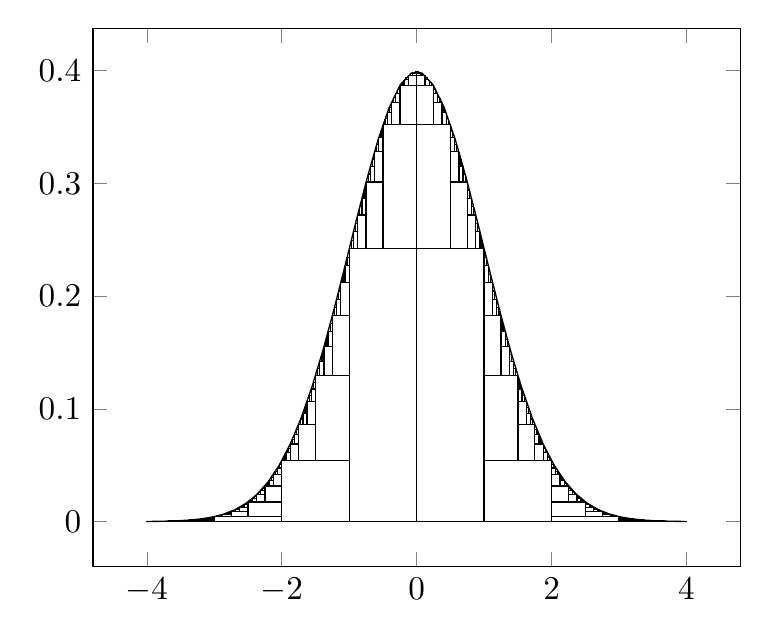
\begin{tikzpicture}[scale=1.2]
\begin{axis}
\addplot[domain=-4:4, samples=50] {e^(-x^2/2)/sqrt(2*pi)};
\draw (axis cs: -4, 0) -- (axis cs: 4, 0);
\draw (axis cs: -4, 0) -- (axis cs: -4, 1.3383022577439575E-4);
\draw (axis cs: -3, 0) -- (axis cs: -3, 1.3383022577439575E-4);
\draw (axis cs: -4, 1.3383022577439575E-4) -- (axis cs: -3, 1.3383022577439575E-4);
\draw (axis cs: -4, 1.3383022577439575E-4) -- (axis cs: -4, 1.338302257719816E-4);
\draw (axis cs: -7/2, 1.3383022577439575E-4) -- (axis cs: -7/2, 1.338302257719816E-4);
\draw (axis cs: -4, 1.338302257719816E-4) -- (axis cs: -7/2, 1.338302257719816E-4);
\draw (axis cs: -7/2, 1.3383022577439575E-4) -- (axis cs: -7/2, 8.726826968250417E-4);
\draw (axis cs: -3, 1.3383022577439575E-4) -- (axis cs: -3, 8.726826968250417E-4);
\draw (axis cs: -7/2, 8.726826968250417E-4) -- (axis cs: -3, 8.726826968250417E-4);
\draw (axis cs: -4, 1.338302257719816E-4) -- (axis cs: -4, 1.3383022577495704E-4);
\draw (axis cs: -15/4, 1.338302257719816E-4) -- (axis cs: -15/4, 1.3383022577495704E-4);
\draw (axis cs: -4, 1.3383022577495704E-4) -- (axis cs: -15/4, 1.3383022577495704E-4);
\draw (axis cs: -15/4, 1.338302257719816E-4) -- (axis cs: -15/4, 3.525956827459561E-4);
\draw (axis cs: -7/2, 1.338302257719816E-4) -- (axis cs: -7/2, 3.525956827459561E-4);
\draw (axis cs: -15/4, 3.525956827459561E-4) -- (axis cs: -7/2, 3.525956827459561E-4);
\draw (axis cs: -7/2, 8.726826968250417E-4) -- (axis cs: -7/2, 8.726826977454657E-4);
\draw (axis cs: -13/4, 8.726826968250417E-4) -- (axis cs: -13/4, 8.726826977454657E-4);
\draw (axis cs: -7/2, 8.726826977454657E-4) -- (axis cs: -13/4, 8.726826977454657E-4);
\draw (axis cs: -13/4, 8.726826968250417E-4) -- (axis cs: -13/4, 0.002029048066730719);
\draw (axis cs: -3, 8.726826968250417E-4) -- (axis cs: -3, 0.002029048066730719);
\draw (axis cs: -13/4, 0.002029048066730719) -- (axis cs: -3, 0.002029048066730719);
\draw (axis cs: -4, 1.3383022577495704E-4) -- (axis cs: -4, 1.338302257727162E-4);
\draw (axis cs: -31/8, 1.3383022577495704E-4) -- (axis cs: -31/8, 1.338302257727162E-4);
\draw (axis cs: -4, 1.338302257727162E-4) -- (axis cs: -31/8, 1.338302257727162E-4);
\draw (axis cs: -31/8, 1.3383022577495704E-4) -- (axis cs: -31/8, 2.189316378817986E-4);
\draw (axis cs: -15/4, 1.3383022577495704E-4) -- (axis cs: -15/4, 2.189316378817986E-4);
\draw (axis cs: -31/8, 2.189316378817986E-4) -- (axis cs: -15/4, 2.189316378817986E-4);
\draw (axis cs: -15/4, 3.525956827459561E-4) -- (axis cs: -15/4, 3.5259568295179194E-4);
\draw (axis cs: -29/8, 3.525956827459561E-4) -- (axis cs: -29/8, 3.5259568295179194E-4);
\draw (axis cs: -15/4, 3.5259568295179194E-4) -- (axis cs: -29/8, 3.5259568295179194E-4);
\draw (axis cs: -29/8, 3.525956827459561E-4) -- (axis cs: -29/8, 5.590615236813285E-4);
\draw (axis cs: -7/2, 3.525956827459561E-4) -- (axis cs: -7/2, 5.590615236813285E-4);
\draw (axis cs: -29/8, 5.590615236813285E-4) -- (axis cs: -7/2, 5.590615236813285E-4);
\draw (axis cs: -7/2, 8.726826977454657E-4) -- (axis cs: -7/2, 8.726826970219815E-4);
\draw (axis cs: -27/8, 8.726826977454657E-4) -- (axis cs: -27/8, 8.726826970219815E-4);
\draw (axis cs: -7/2, 8.726826970219815E-4) -- (axis cs: -27/8, 8.726826970219815E-4);
\draw (axis cs: -27/8, 8.726826977454657E-4) -- (axis cs: -27/8, 0.0013411188787273267);
\draw (axis cs: -13/4, 8.726826977454657E-4) -- (axis cs: -13/4, 0.0013411188787273267);
\draw (axis cs: -27/8, 0.0013411188787273267) -- (axis cs: -13/4, 0.0013411188787273267);
\draw (axis cs: -13/4, 0.002029048066730719) -- (axis cs: -13/4, 0.0020290480646332917);
\draw (axis cs: -25/8, 0.002029048066730719) -- (axis cs: -25/8, 0.0020290480646332917);
\draw (axis cs: -13/4, 0.0020290480646332917) -- (axis cs: -25/8, 0.0020290480646332917);
\draw (axis cs: -25/8, 0.002029048066730719) -- (axis cs: -25/8, 0.0030222580445213106);
\draw (axis cs: -3, 0.002029048066730719) -- (axis cs: -3, 0.0030222580445213106);
\draw (axis cs: -25/8, 0.0030222580445213106) -- (axis cs: -3, 0.0030222580445213106);
\draw (axis cs: -4, 1.338302257727162E-4) -- (axis cs: -4, 1.338302257755516E-4);
\draw (axis cs: -63/16, 1.338302257727162E-4) -- (axis cs: -63/16, 1.338302257755516E-4);
\draw (axis cs: -4, 1.338302257755516E-4) -- (axis cs: -63/16, 1.338302257755516E-4);
\draw (axis cs: -63/16, 1.338302257727162E-4) -- (axis cs: -63/16, 1.7150611128694776E-4);
\draw (axis cs: -31/8, 1.338302257727162E-4) -- (axis cs: -31/8, 1.7150611128694776E-4);
\draw (axis cs: -63/16, 1.7150611128694776E-4) -- (axis cs: -31/8, 1.7150611128694776E-4);
\draw (axis cs: -31/8, 2.189316378817986E-4) -- (axis cs: -31/8, 2.1893163795207372E-4);
\draw (axis cs: -61/16, 2.189316378817986E-4) -- (axis cs: -61/16, 2.1893163795207372E-4);
\draw (axis cs: -31/8, 2.1893163795207372E-4) -- (axis cs: -61/16, 2.1893163795207372E-4);
\draw (axis cs: -61/16, 2.189316378817986E-4) -- (axis cs: -61/16, 2.783818969778259E-4);
\draw (axis cs: -15/4, 2.189316378817986E-4) -- (axis cs: -15/4, 2.783818969778259E-4);
\draw (axis cs: -61/16, 2.783818969778259E-4) -- (axis cs: -15/4, 2.783818969778259E-4);
\draw (axis cs: -15/4, 3.5259568295179194E-4) -- (axis cs: -15/4, 3.525956827885839E-4);
\draw (axis cs: -59/16, 3.5259568295179194E-4) -- (axis cs: -59/16, 3.525956827885839E-4);
\draw (axis cs: -15/4, 3.525956827885839E-4) -- (axis cs: -59/16, 3.525956827885839E-4);
\draw (axis cs: -59/16, 3.5259568295179194E-4) -- (axis cs: -59/16, 4.4485300506178784E-4);
\draw (axis cs: -29/8, 3.5259568295179194E-4) -- (axis cs: -29/8, 4.4485300506178784E-4);
\draw (axis cs: -59/16, 4.4485300506178784E-4) -- (axis cs: -29/8, 4.4485300506178784E-4);
\draw (axis cs: -29/8, 5.590615236813285E-4) -- (axis cs: -29/8, 5.590615233489036E-4);
\draw (axis cs: -57/16, 5.590615236813285E-4) -- (axis cs: -57/16, 5.590615233489036E-4);
\draw (axis cs: -29/8, 5.590615233489036E-4) -- (axis cs: -57/16, 5.590615233489036E-4);
\draw (axis cs: -57/16, 5.590615236813285E-4) -- (axis cs: -57/16, 6.99852012164985E-4);
\draw (axis cs: -7/2, 5.590615236813285E-4) -- (axis cs: -7/2, 6.99852012164985E-4);
\draw (axis cs: -57/16, 6.99852012164985E-4) -- (axis cs: -7/2, 6.99852012164985E-4);
\draw (axis cs: -7/2, 8.726826970219815E-4) -- (axis cs: -7/2, 8.726826979047949E-4);
\draw (axis cs: -55/16, 8.726826970219815E-4) -- (axis cs: -55/16, 8.726826979047949E-4);
\draw (axis cs: -7/2, 8.726826979047949E-4) -- (axis cs: -55/16, 8.726826979047949E-4);
\draw (axis cs: -55/16, 8.726826970219815E-4) -- (axis cs: -55/16, 0.0010839520026024215);
\draw (axis cs: -27/8, 8.726826970219815E-4) -- (axis cs: -27/8, 0.0010839520026024215);
\draw (axis cs: -55/16, 0.0010839520026024215) -- (axis cs: -27/8, 0.0010839520026024215);
\draw (axis cs: -27/8, 0.0013411188787273267) -- (axis cs: -27/8, 0.0013411188774714465);
\draw (axis cs: -53/16, 0.0013411188787273267) -- (axis cs: -53/16, 0.0013411188774714465);
\draw (axis cs: -27/8, 0.0013411188774714465) -- (axis cs: -53/16, 0.0013411188774714465);
\draw (axis cs: -53/16, 0.0013411188787273267) -- (axis cs: -53/16, 0.0016528294268795848);
\draw (axis cs: -13/4, 0.0013411188787273267) -- (axis cs: -13/4, 0.0016528294268795848);
\draw (axis cs: -53/16, 0.0016528294268795848) -- (axis cs: -13/4, 0.0016528294268795848);
\draw (axis cs: -13/4, 0.0020290480646332917) -- (axis cs: -13/4, 0.002029048067287304);
\draw (axis cs: -51/16, 0.0020290480646332917) -- (axis cs: -51/16, 0.002029048067287304);
\draw (axis cs: -13/4, 0.002029048067287304) -- (axis cs: -51/16, 0.002029048067287304);
\draw (axis cs: -51/16, 0.0020290480646332917) -- (axis cs: -51/16, 0.00248119084808154);
\draw (axis cs: -25/8, 0.0020290480646332917) -- (axis cs: -25/8, 0.00248119084808154);
\draw (axis cs: -51/16, 0.00248119084808154) -- (axis cs: -25/8, 0.00248119084808154);
\draw (axis cs: -25/8, 0.0030222580445213106) -- (axis cs: -25/8, 0.003022258049502977);
\draw (axis cs: -49/16, 0.0030222580445213106) -- (axis cs: -49/16, 0.003022258049502977);
\draw (axis cs: -25/8, 0.003022258049502977) -- (axis cs: -49/16, 0.003022258049502977);
\draw (axis cs: -49/16, 0.0030222580445213106) -- (axis cs: -49/16, 0.0036669623631740054);
\draw (axis cs: -3, 0.0030222580445213106) -- (axis cs: -3, 0.0036669623631740054);
\draw (axis cs: -49/16, 0.0036669623631740054) -- (axis cs: -3, 0.0036669623631740054);
\draw (axis cs: -4, 1.338302257755516E-4) -- (axis cs: -4, 1.3383022577349429E-4);
\draw (axis cs: -127/32, 1.338302257755516E-4) -- (axis cs: -127/32, 1.3383022577349429E-4);
\draw (axis cs: -4, 1.3383022577349429E-4) -- (axis cs: -127/32, 1.3383022577349429E-4);
\draw (axis cs: -127/32, 1.338302257755516E-4) -- (axis cs: -127/32, 1.5157548380131383E-4);
\draw (axis cs: -63/16, 1.338302257755516E-4) -- (axis cs: -63/16, 1.5157548380131383E-4);
\draw (axis cs: -127/32, 1.5157548380131383E-4) -- (axis cs: -63/16, 1.5157548380131383E-4);
\draw (axis cs: -63/16, 1.7150611128694776E-4) -- (axis cs: -63/16, 1.7150611126648675E-4);
\draw (axis cs: -125/32, 1.7150611128694776E-4) -- (axis cs: -125/32, 1.7150611126648675E-4);
\draw (axis cs: -63/16, 1.7150611126648675E-4) -- (axis cs: -125/32, 1.7150611126648675E-4);
\draw (axis cs: -125/32, 1.7150611128694776E-4) -- (axis cs: -125/32, 1.938679959484055E-4);
\draw (axis cs: -31/8, 1.7150611128694776E-4) -- (axis cs: -31/8, 1.938679959484055E-4);
\draw (axis cs: -125/32, 1.938679959484055E-4) -- (axis cs: -31/8, 1.938679959484055E-4);
\draw (axis cs: -31/8, 2.1893163795207372E-4) -- (axis cs: -31/8, 2.1893163789547392E-4);
\draw (axis cs: -123/32, 2.1893163795207372E-4) -- (axis cs: -123/32, 2.1893163789547392E-4);
\draw (axis cs: -31/8, 2.1893163789547392E-4) -- (axis cs: -123/32, 2.1893163789547392E-4);
\draw (axis cs: -123/32, 2.1893163795207372E-4) -- (axis cs: -123/32, 2.4699423459166776E-4);
\draw (axis cs: -61/16, 2.1893163795207372E-4) -- (axis cs: -61/16, 2.4699423459166776E-4);
\draw (axis cs: -123/32, 2.4699423459166776E-4) -- (axis cs: -61/16, 2.4699423459166776E-4);
\draw (axis cs: -61/16, 2.783818969778259E-4) -- (axis cs: -61/16, 2.783818968854738E-4);
\draw (axis cs: -121/32, 2.783818969778259E-4) -- (axis cs: -121/32, 2.783818968854738E-4);
\draw (axis cs: -61/16, 2.783818968854738E-4) -- (axis cs: -121/32, 2.783818968854738E-4);
\draw (axis cs: -121/32, 2.783818969778259E-4) -- (axis cs: -121/32, 3.134520019157421E-4);
\draw (axis cs: -15/4, 2.783818969778259E-4) -- (axis cs: -15/4, 3.134520019157421E-4);
\draw (axis cs: -121/32, 3.134520019157421E-4) -- (axis cs: -15/4, 3.134520019157421E-4);
\draw (axis cs: -15/4, 3.525956827885839E-4) -- (axis cs: -15/4, 3.525956829862783E-4);
\draw (axis cs: -119/32, 3.525956827885839E-4) -- (axis cs: -119/32, 3.525956829862783E-4);
\draw (axis cs: -15/4, 3.525956829862783E-4) -- (axis cs: -119/32, 3.525956829862783E-4);
\draw (axis cs: -119/32, 3.525956827885839E-4) -- (axis cs: -119/32, 3.962404584351427E-4);
\draw (axis cs: -59/16, 3.525956827885839E-4) -- (axis cs: -59/16, 3.962404584351427E-4);
\draw (axis cs: -119/32, 3.962404584351427E-4) -- (axis cs: -59/16, 3.962404584351427E-4);
\draw (axis cs: -59/16, 4.4485300506178784E-4) -- (axis cs: -59/16, 4.4485300482601024E-4);
\draw (axis cs: -117/32, 4.4485300506178784E-4) -- (axis cs: -117/32, 4.4485300482601024E-4);
\draw (axis cs: -59/16, 4.4485300482601024E-4) -- (axis cs: -117/32, 4.4485300482601024E-4);
\draw (axis cs: -117/32, 4.4485300506178784E-4) -- (axis cs: -117/32, 4.989420690804763E-4);
\draw (axis cs: -29/8, 4.4485300506178784E-4) -- (axis cs: -29/8, 4.989420690804763E-4);
\draw (axis cs: -117/32, 4.989420690804763E-4) -- (axis cs: -29/8, 4.989420690804763E-4);
\draw (axis cs: -29/8, 5.590615233489036E-4) -- (axis cs: -29/8, 5.590615237668537E-4);
\draw (axis cs: -115/32, 5.590615233489036E-4) -- (axis cs: -115/32, 5.590615237668537E-4);
\draw (axis cs: -29/8, 5.590615237668537E-4) -- (axis cs: -115/32, 5.590615237668537E-4);
\draw (axis cs: -115/32, 5.590615233489036E-4) -- (axis cs: -115/32, 6.258135581015341E-4);
\draw (axis cs: -57/16, 5.590615233489036E-4) -- (axis cs: -57/16, 6.258135581015341E-4);
\draw (axis cs: -115/32, 6.258135581015341E-4) -- (axis cs: -57/16, 6.258135581015341E-4);
\draw (axis cs: -57/16, 6.99852012164985E-4) -- (axis cs: -57/16, 6.998520128349937E-4);
\draw (axis cs: -113/32, 6.99852012164985E-4) -- (axis cs: -113/32, 6.998520128349937E-4);
\draw (axis cs: -57/16, 6.998520128349937E-4) -- (axis cs: -113/32, 6.998520128349937E-4);
\draw (axis cs: -113/32, 6.99852012164985E-4) -- (axis cs: -113/32, 7.818858407131201E-4);
\draw (axis cs: -7/2, 6.99852012164985E-4) -- (axis cs: -7/2, 7.818858407131201E-4);
\draw (axis cs: -113/32, 7.818858407131201E-4) -- (axis cs: -7/2, 7.818858407131201E-4);
\draw (axis cs: -7/2, 8.726826979047949E-4) -- (axis cs: -7/2, 8.726826972305451E-4);
\draw (axis cs: -111/32, 8.726826979047949E-4) -- (axis cs: -111/32, 8.726826972305451E-4);
\draw (axis cs: -7/2, 8.726826972305451E-4) -- (axis cs: -111/32, 8.726826972305451E-4);
\draw (axis cs: -111/32, 8.726826979047949E-4) -- (axis cs: -111/32, 9.730726504887151E-4);
\draw (axis cs: -55/16, 8.726826979047949E-4) -- (axis cs: -55/16, 9.730726504887151E-4);
\draw (axis cs: -111/32, 9.730726504887151E-4) -- (axis cs: -55/16, 9.730726504887151E-4);
\draw (axis cs: -55/16, 0.0010839520026024215) -- (axis cs: -55/16, 0.0010839520015470169);
\draw (axis cs: -109/32, 0.0010839520026024215) -- (axis cs: -109/32, 0.0010839520015470169);
\draw (axis cs: -55/16, 0.0010839520015470169) -- (axis cs: -109/32, 0.0010839520015470169);
\draw (axis cs: -109/32, 0.0010839520026024215) -- (axis cs: -109/32, 0.0012062872049105834);
\draw (axis cs: -27/8, 0.0010839520026024215) -- (axis cs: -27/8, 0.0012062872049105834);
\draw (axis cs: -109/32, 0.0012062872049105834) -- (axis cs: -27/8, 0.0012062872049105834);
\draw (axis cs: -27/8, 0.0013411188774714465) -- (axis cs: -27/8, 0.0013411188790363948);
\draw (axis cs: -107/32, 0.0013411188774714465) -- (axis cs: -107/32, 0.0013411188790363948);
\draw (axis cs: -27/8, 0.0013411188790363948) -- (axis cs: -107/32, 0.0013411188790363948);
\draw (axis cs: -107/32, 0.0013411188774714465) -- (axis cs: -107/32, 0.0014895658752694212);
\draw (axis cs: -53/16, 0.0013411188774714465) -- (axis cs: -53/16, 0.0014895658752694212);
\draw (axis cs: -107/32, 0.0014895658752694212) -- (axis cs: -53/16, 0.0014895658752694212);
\draw (axis cs: -53/16, 0.0016528294268795848) -- (axis cs: -53/16, 0.001652829429114738);
\draw (axis cs: -105/32, 0.0016528294268795848) -- (axis cs: -105/32, 0.001652829429114738);
\draw (axis cs: -53/16, 0.001652829429114738) -- (axis cs: -105/32, 0.001652829429114738);
\draw (axis cs: -105/32, 0.0016528294268795848) -- (axis cs: -105/32, 0.0018321973212320946);
\draw (axis cs: -13/4, 0.0016528294268795848) -- (axis cs: -13/4, 0.0018321973212320946);
\draw (axis cs: -105/32, 0.0018321973212320946) -- (axis cs: -13/4, 0.0018321973212320946);
\draw (axis cs: -13/4, 0.002029048067287304) -- (axis cs: -13/4, 0.002029048065361871);
\draw (axis cs: -103/32, 0.002029048067287304) -- (axis cs: -103/32, 0.002029048065361871);
\draw (axis cs: -13/4, 0.002029048065361871) -- (axis cs: -103/32, 0.002029048065361871);
\draw (axis cs: -103/32, 0.002029048067287304) -- (axis cs: -103/32, 0.002244855083569142);
\draw (axis cs: -51/16, 0.002029048067287304) -- (axis cs: -51/16, 0.002244855083569142);
\draw (axis cs: -103/32, 0.002244855083569142) -- (axis cs: -51/16, 0.002244855083569142);
\draw (axis cs: -51/16, 0.00248119084808154) -- (axis cs: -51/16, 0.0024811908452780345);
\draw (axis cs: -101/32, 0.00248119084808154) -- (axis cs: -101/32, 0.0024811908452780345);
\draw (axis cs: -51/16, 0.0024811908452780345) -- (axis cs: -101/32, 0.0024811908452780345);
\draw (axis cs: -101/32, 0.00248119084808154) -- (axis cs: -101/32, 0.0027397309388828904);
\draw (axis cs: -25/8, 0.00248119084808154) -- (axis cs: -25/8, 0.0027397309388828904);
\draw (axis cs: -101/32, 0.0027397309388828904) -- (axis cs: -25/8, 0.0027397309388828904);
\draw (axis cs: -25/8, 0.003022258049502977) -- (axis cs: -25/8, 0.0030222580455647884);
\draw (axis cs: -99/32, 0.003022258049502977) -- (axis cs: -99/32, 0.0030222580455647884);
\draw (axis cs: -25/8, 0.0030222580455647884) -- (axis cs: -99/32, 0.0030222580455647884);
\draw (axis cs: -99/32, 0.003022258049502977) -- (axis cs: -99/32, 0.0033306657796143787);
\draw (axis cs: -49/16, 0.003022258049502977) -- (axis cs: -49/16, 0.0033306657796143787);
\draw (axis cs: -99/32, 0.0033306657796143787) -- (axis cs: -49/16, 0.0033306657796143787);
\draw (axis cs: -49/16, 0.0036669623631740054) -- (axis cs: -49/16, 0.0036669623579181037);
\draw (axis cs: -97/32, 0.0036669623631740054) -- (axis cs: -97/32, 0.0036669623579181037);
\draw (axis cs: -49/16, 0.0036669623579181037) -- (axis cs: -97/32, 0.0036669623579181037);
\draw (axis cs: -97/32, 0.0036669623631740054) -- (axis cs: -97/32, 0.0040332740584328826);
\draw (axis cs: -3, 0.0036669623631740054) -- (axis cs: -3, 0.0040332740584328826);
\draw (axis cs: -97/32, 0.0040332740584328826) -- (axis cs: -3, 0.0040332740584328826);
\draw (axis cs: -3, 0) -- (axis cs: -3, 0.004431848412174211);
\draw (axis cs: -2, 0) -- (axis cs: -2, 0.004431848412174211);
\draw (axis cs: -3, 0.004431848412174211) -- (axis cs: -2, 0.004431848412174211);
\draw (axis cs: -3, 0.004431848412174211) -- (axis cs: -3, 0.0044318484121142546);
\draw (axis cs: -5/2, 0.004431848412174211) -- (axis cs: -5/2, 0.0044318484121142546);
\draw (axis cs: -3, 0.0044318484121142546) -- (axis cs: -5/2, 0.0044318484121142546);
\draw (axis cs: -5/2, 0.004431848412174211) -- (axis cs: -5/2, 0.017528300519095555);
\draw (axis cs: -2, 0.004431848412174211) -- (axis cs: -2, 0.017528300519095555);
\draw (axis cs: -5/2, 0.017528300519095555) -- (axis cs: -2, 0.017528300519095555);
\draw (axis cs: -3, 0.0044318484121142546) -- (axis cs: -3, 0.004431848412188154);
\draw (axis cs: -11/4, 0.0044318484121142546) -- (axis cs: -11/4, 0.004431848412188154);
\draw (axis cs: -3, 0.004431848412188154) -- (axis cs: -11/4, 0.004431848412188154);
\draw (axis cs: -11/4, 0.0044318484121142546) -- (axis cs: -11/4, 0.009093562508749794);
\draw (axis cs: -5/2, 0.0044318484121142546) -- (axis cs: -5/2, 0.009093562508749794);
\draw (axis cs: -11/4, 0.009093562508749794) -- (axis cs: -5/2, 0.009093562508749794);
\draw (axis cs: -5/2, 0.017528300519095555) -- (axis cs: -5/2, 0.017528300532300707);
\draw (axis cs: -9/4, 0.017528300519095555) -- (axis cs: -9/4, 0.017528300532300707);
\draw (axis cs: -5/2, 0.017528300532300707) -- (axis cs: -9/4, 0.017528300532300707);
\draw (axis cs: -9/4, 0.017528300519095555) -- (axis cs: -9/4, 0.031739651937800026);
\draw (axis cs: -2, 0.017528300519095555) -- (axis cs: -2, 0.031739651937800026);
\draw (axis cs: -9/4, 0.031739651937800026) -- (axis cs: -2, 0.031739651937800026);
\draw (axis cs: -3, 0.004431848412188154) -- (axis cs: -3, 0.004431848412132499);
\draw (axis cs: -23/8, 0.004431848412188154) -- (axis cs: -23/8, 0.004431848412132499);
\draw (axis cs: -3, 0.004431848412132499) -- (axis cs: -23/8, 0.004431848412132499);
\draw (axis cs: -23/8, 0.004431848412188154) -- (axis cs: -23/8, 0.006398120313264456);
\draw (axis cs: -11/4, 0.004431848412188154) -- (axis cs: -11/4, 0.006398120313264456);
\draw (axis cs: -23/8, 0.006398120313264456) -- (axis cs: -11/4, 0.006398120313264456);
\draw (axis cs: -11/4, 0.009093562508749794) -- (axis cs: -11/4, 0.00909356251264275);
\draw (axis cs: -21/8, 0.009093562508749794) -- (axis cs: -21/8, 0.00909356251264275);
\draw (axis cs: -11/4, 0.00909356251264275) -- (axis cs: -21/8, 0.00909356251264275);
\draw (axis cs: -21/8, 0.009093562508749794) -- (axis cs: -21/8, 0.012724181620715534);
\draw (axis cs: -5/2, 0.009093562508749794) -- (axis cs: -5/2, 0.012724181620715534);
\draw (axis cs: -21/8, 0.012724181620715534) -- (axis cs: -5/2, 0.012724181620715534);
\draw (axis cs: -5/2, 0.017528300532300707) -- (axis cs: -5/2, 0.017528300521921024);
\draw (axis cs: -19/8, 0.017528300532300707) -- (axis cs: -19/8, 0.017528300521921024);
\draw (axis cs: -5/2, 0.017528300521921024) -- (axis cs: -19/8, 0.017528300521921024);
\draw (axis cs: -19/8, 0.017528300532300707) -- (axis cs: -19/8, 0.023771900895236606);
\draw (axis cs: -9/4, 0.017528300532300707) -- (axis cs: -9/4, 0.023771900895236606);
\draw (axis cs: -19/8, 0.023771900895236606) -- (axis cs: -9/4, 0.023771900895236606);
\draw (axis cs: -9/4, 0.031739651937800026) -- (axis cs: -9/4, 0.03173965191508592);
\draw (axis cs: -17/8, 0.031739651937800026) -- (axis cs: -17/8, 0.03173965191508592);
\draw (axis cs: -9/4, 0.03173965191508592) -- (axis cs: -17/8, 0.03173965191508592);
\draw (axis cs: -17/8, 0.031739651937800026) -- (axis cs: -17/8, 0.04172098534385047);
\draw (axis cs: -2, 0.031739651937800026) -- (axis cs: -2, 0.04172098534385047);
\draw (axis cs: -17/8, 0.04172098534385047) -- (axis cs: -2, 0.04172098534385047);
\draw (axis cs: -3, 0.004431848412132499) -- (axis cs: -3, 0.004431848412202919);
\draw (axis cs: -47/16, 0.004431848412132499) -- (axis cs: -47/16, 0.004431848412202919);
\draw (axis cs: -3, 0.004431848412202919) -- (axis cs: -47/16, 0.004431848412202919);
\draw (axis cs: -47/16, 0.004431848412132499) -- (axis cs: -47/16, 0.005335398733726687);
\draw (axis cs: -23/8, 0.004431848412132499) -- (axis cs: -23/8, 0.005335398733726687);
\draw (axis cs: -47/16, 0.005335398733726687) -- (axis cs: -23/8, 0.005335398733726687);
\draw (axis cs: -23/8, 0.006398120313264456) -- (axis cs: -23/8, 0.006398120314788203);
\draw (axis cs: -45/16, 0.006398120313264456) -- (axis cs: -45/16, 0.006398120314788203);
\draw (axis cs: -23/8, 0.006398120314788203) -- (axis cs: -45/16, 0.006398120314788203);
\draw (axis cs: -45/16, 0.006398120313264456) -- (axis cs: -45/16, 0.007642605826431574);
\draw (axis cs: -11/4, 0.006398120313264456) -- (axis cs: -11/4, 0.007642605826431574);
\draw (axis cs: -45/16, 0.007642605826431574) -- (axis cs: -11/4, 0.007642605826431574);
\draw (axis cs: -11/4, 0.00909356251264275) -- (axis cs: -11/4, 0.009093562509556006);
\draw (axis cs: -43/16, 0.00909356251264275) -- (axis cs: -43/16, 0.009093562509556006);
\draw (axis cs: -11/4, 0.009093562509556006) -- (axis cs: -43/16, 0.009093562509556006);
\draw (axis cs: -43/16, 0.00909356251264275) -- (axis cs: -43/16, 0.010777801717027505);
\draw (axis cs: -21/8, 0.00909356251264275) -- (axis cs: -21/8, 0.010777801717027505);
\draw (axis cs: -43/16, 0.010777801717027505) -- (axis cs: -21/8, 0.010777801717027505);
\draw (axis cs: -21/8, 0.012724181620715534) -- (axis cs: -21/8, 0.01272418161523674);
\draw (axis cs: -41/16, 0.012724181620715534) -- (axis cs: -41/16, 0.01272418161523674);
\draw (axis cs: -21/8, 0.01272418161523674) -- (axis cs: -41/16, 0.01272418161523674);
\draw (axis cs: -41/16, 0.012724181620715534) -- (axis cs: -41/16, 0.014963495804646555);
\draw (axis cs: -5/2, 0.012724181620715534) -- (axis cs: -5/2, 0.014963495804646555);
\draw (axis cs: -41/16, 0.014963495804646555) -- (axis cs: -5/2, 0.014963495804646555);
\draw (axis cs: -5/2, 0.017528300521921024) -- (axis cs: -5/2, 0.01752830053458658);
\draw (axis cs: -39/16, 0.017528300521921024) -- (axis cs: -39/16, 0.01752830053458658);
\draw (axis cs: -5/2, 0.01752830053458658) -- (axis cs: -39/16, 0.01752830053458658);
\draw (axis cs: -39/16, 0.017528300521921024) -- (axis cs: -39/16, 0.02045267381944624);
\draw (axis cs: -19/8, 0.017528300521921024) -- (axis cs: -19/8, 0.02045267381944624);
\draw (axis cs: -39/16, 0.02045267381944624) -- (axis cs: -19/8, 0.02045267381944624);
\draw (axis cs: -19/8, 0.023771900895236606) -- (axis cs: -19/8, 0.023771900879571463);
\draw (axis cs: -37/16, 0.023771900895236606) -- (axis cs: -37/16, 0.023771900879571463);
\draw (axis cs: -19/8, 0.023771900879571463) -- (axis cs: -37/16, 0.023771900879571463);
\draw (axis cs: -37/16, 0.023771900895236606) -- (axis cs: -37/16, 0.02752208085490523);
\draw (axis cs: -9/4, 0.023771900895236606) -- (axis cs: -9/4, 0.02752208085490523);
\draw (axis cs: -37/16, 0.02752208085490523) -- (axis cs: -9/4, 0.02752208085490523);
\draw (axis cs: -9/4, 0.03173965191508592) -- (axis cs: -9/4, 0.031739651943827586);
\draw (axis cs: -35/16, 0.03173965191508592) -- (axis cs: -35/16, 0.031739651943827586);
\draw (axis cs: -9/4, 0.031739651943827586) -- (axis cs: -35/16, 0.031739651943827586);
\draw (axis cs: -35/16, 0.03173965191508592) -- (axis cs: -35/16, 0.03646083329698946);
\draw (axis cs: -17/8, 0.03173965191508592) -- (axis cs: -17/8, 0.03646083329698946);
\draw (axis cs: -35/16, 0.03646083329698946) -- (axis cs: -17/8, 0.03646083329698946);
\draw (axis cs: -17/8, 0.04172098534385047) -- (axis cs: -17/8, 0.04172098539061392);
\draw (axis cs: -33/16, 0.04172098534385047) -- (axis cs: -33/16, 0.04172098539061392);
\draw (axis cs: -17/8, 0.04172098539061392) -- (axis cs: -33/16, 0.04172098539061392);
\draw (axis cs: -33/16, 0.04172098534385047) -- (axis cs: -33/16, 0.0475538914080623);
\draw (axis cs: -2, 0.04172098534385047) -- (axis cs: -2, 0.0475538914080623);
\draw (axis cs: -33/16, 0.0475538914080623) -- (axis cs: -2, 0.0475538914080623);
\draw (axis cs: -3, 0.004431848412202919) -- (axis cs: -3, 0.004431848412151822);
\draw (axis cs: -95/32, 0.004431848412202919) -- (axis cs: -95/32, 0.004431848412151822);
\draw (axis cs: -3, 0.004431848412151822) -- (axis cs: -95/32, 0.004431848412151822);
\draw (axis cs: -95/32, 0.004431848412202919) -- (axis cs: -95/32, 0.004865057159669394);
\draw (axis cs: -47/16, 0.004431848412202919) -- (axis cs: -47/16, 0.004865057159669394);
\draw (axis cs: -95/32, 0.004865057159669394) -- (axis cs: -47/16, 0.004865057159669394);
\draw (axis cs: -47/16, 0.005335398733726687) -- (axis cs: -47/16, 0.005335398733251823);
\draw (axis cs: -93/32, 0.005335398733726687) -- (axis cs: -93/32, 0.005335398733251823);
\draw (axis cs: -47/16, 0.005335398733251823) -- (axis cs: -93/32, 0.005335398733251823);
\draw (axis cs: -93/32, 0.005335398733726687) -- (axis cs: -93/32, 0.005845500471043691);
\draw (axis cs: -23/8, 0.005335398733726687) -- (axis cs: -23/8, 0.005845500471043691);
\draw (axis cs: -93/32, 0.005845500471043691) -- (axis cs: -23/8, 0.005845500471043691);
\draw (axis cs: -23/8, 0.006398120314788203) -- (axis cs: -23/8, 0.0063981203135609725);
\draw (axis cs: -91/32, 0.006398120314788203) -- (axis cs: -91/32, 0.0063981203135609725);
\draw (axis cs: -23/8, 0.0063981203135609725) -- (axis cs: -91/32, 0.0063981203135609725);
\draw (axis cs: -91/32, 0.006398120314788203) -- (axis cs: -91/32, 0.006996148024288882);
\draw (axis cs: -45/16, 0.006398120314788203) -- (axis cs: -45/16, 0.006996148024288882);
\draw (axis cs: -91/32, 0.006996148024288882) -- (axis cs: -45/16, 0.006996148024288882);
\draw (axis cs: -45/16, 0.007642605826431574) -- (axis cs: -45/16, 0.007642605824561196);
\draw (axis cs: -89/32, 0.007642605826431574) -- (axis cs: -89/32, 0.007642605824561196);
\draw (axis cs: -45/16, 0.007642605824561196) -- (axis cs: -89/32, 0.007642605824561196);
\draw (axis cs: -89/32, 0.007642605826431574) -- (axis cs: -89/32, 0.008340648450385625);
\draw (axis cs: -11/4, 0.007642605826431574) -- (axis cs: -11/4, 0.008340648450385625);
\draw (axis cs: -89/32, 0.008340648450385625) -- (axis cs: -11/4, 0.008340648450385625);
\draw (axis cs: -11/4, 0.009093562509556006) -- (axis cs: -11/4, 0.009093562513294988);
\draw (axis cs: -87/32, 0.009093562509556006) -- (axis cs: -87/32, 0.009093562513294988);
\draw (axis cs: -11/4, 0.009093562513294988) -- (axis cs: -87/32, 0.009093562513294988);
\draw (axis cs: -87/32, 0.009093562509556006) -- (axis cs: -87/32, 0.009904765112088453);
\draw (axis cs: -43/16, 0.009093562509556006) -- (axis cs: -43/16, 0.009904765112088453);
\draw (axis cs: -87/32, 0.009904765112088453) -- (axis cs: -43/16, 0.009904765112088453);
\draw (axis cs: -43/16, 0.010777801717027505) -- (axis cs: -43/16, 0.010777801712864257);
\draw (axis cs: -85/32, 0.010777801717027505) -- (axis cs: -85/32, 0.010777801712864257);
\draw (axis cs: -43/16, 0.010777801712864257) -- (axis cs: -85/32, 0.010777801712864257);
\draw (axis cs: -85/32, 0.010777801717027505) -- (axis cs: -85/32, 0.011716343127226523);
\draw (axis cs: -21/8, 0.010777801717027505) -- (axis cs: -21/8, 0.011716343127226523);
\draw (axis cs: -85/32, 0.011716343127226523) -- (axis cs: -21/8, 0.011716343127226523);
\draw (axis cs: -21/8, 0.01272418161523674) -- (axis cs: -21/8, 0.012724181622125099);
\draw (axis cs: -83/32, 0.01272418161523674) -- (axis cs: -83/32, 0.012724181622125099);
\draw (axis cs: -21/8, 0.012724181622125099) -- (axis cs: -83/32, 0.012724181622125099);
\draw (axis cs: -83/32, 0.01272418161523674) -- (axis cs: -83/32, 0.013805226005016956);
\draw (axis cs: -41/16, 0.01272418161523674) -- (axis cs: -41/16, 0.013805226005016956);
\draw (axis cs: -83/32, 0.013805226005016956) -- (axis cs: -41/16, 0.013805226005016956);
\draw (axis cs: -41/16, 0.014963495804646555) -- (axis cs: -41/16, 0.014963495814950807);
\draw (axis cs: -81/32, 0.014963495804646555) -- (axis cs: -81/32, 0.014963495814950807);
\draw (axis cs: -41/16, 0.014963495814950807) -- (axis cs: -81/32, 0.014963495814950807);
\draw (axis cs: -81/32, 0.014963495804646555) -- (axis cs: -81/32, 0.016203114331012073);
\draw (axis cs: -5/2, 0.014963495804646555) -- (axis cs: -5/2, 0.016203114331012073);
\draw (axis cs: -81/32, 0.016203114331012073) -- (axis cs: -5/2, 0.016203114331012073);
\draw (axis cs: -5/2, 0.01752830053458658) -- (axis cs: -5/2, 0.017528300524913245);
\draw (axis cs: -79/32, 0.01752830053458658) -- (axis cs: -79/32, 0.017528300524913245);
\draw (axis cs: -5/2, 0.017528300524913245) -- (axis cs: -79/32, 0.017528300524913245);
\draw (axis cs: -79/32, 0.01752830053458658) -- (axis cs: -79/32, 0.018943359845972896);
\draw (axis cs: -39/16, 0.01752830053458658) -- (axis cs: -39/16, 0.018943359845972896);
\draw (axis cs: -79/32, 0.018943359845972896) -- (axis cs: -39/16, 0.018943359845972896);
\draw (axis cs: -39/16, 0.02045267381944624) -- (axis cs: -39/16, 0.020452673805325384);
\draw (axis cs: -77/32, 0.02045267381944624) -- (axis cs: -77/32, 0.020452673805325384);
\draw (axis cs: -39/16, 0.020452673805325384) -- (axis cs: -77/32, 0.020452673805325384);
\draw (axis cs: -77/32, 0.02045267381944624) -- (axis cs: -77/32, 0.022060688331219873);
\draw (axis cs: -19/8, 0.02045267381944624) -- (axis cs: -19/8, 0.022060688331219873);
\draw (axis cs: -77/32, 0.022060688331219873) -- (axis cs: -19/8, 0.022060688331219873);
\draw (axis cs: -19/8, 0.023771900879571463) -- (axis cs: -19/8, 0.02377190089909175);
\draw (axis cs: -75/32, 0.023771900879571463) -- (axis cs: -75/32, 0.02377190089909175);
\draw (axis cs: -19/8, 0.02377190089909175) -- (axis cs: -75/32, 0.02377190089909175);
\draw (axis cs: -75/32, 0.023771900879571463) -- (axis cs: -75/32, 0.025590846204343713);
\draw (axis cs: -37/16, 0.023771900879571463) -- (axis cs: -37/16, 0.025590846204343713);
\draw (axis cs: -75/32, 0.025590846204343713) -- (axis cs: -37/16, 0.025590846204343713);
\draw (axis cs: -37/16, 0.02752208085490523) -- (axis cs: -37/16, 0.027522080880888054);
\draw (axis cs: -73/32, 0.02752208085490523) -- (axis cs: -73/32, 0.027522080880888054);
\draw (axis cs: -37/16, 0.027522080880888054) -- (axis cs: -73/32, 0.027522080880888054);
\draw (axis cs: -73/32, 0.02752208085490523) -- (axis cs: -73/32, 0.02957016658183054);
\draw (axis cs: -9/4, 0.02752208085490523) -- (axis cs: -9/4, 0.02957016658183054);
\draw (axis cs: -73/32, 0.02957016658183054) -- (axis cs: -9/4, 0.02957016658183054);
\draw (axis cs: -9/4, 0.031739651943827586) -- (axis cs: -9/4, 0.03173965192297608);
\draw (axis cs: -71/32, 0.031739651943827586) -- (axis cs: -71/32, 0.03173965192297608);
\draw (axis cs: -9/4, 0.03173965192297608) -- (axis cs: -71/32, 0.03173965192297608);
\draw (axis cs: -71/32, 0.031739651943827586) -- (axis cs: -71/32, 0.034035053103857585);
\draw (axis cs: -35/16, 0.031739651943827586) -- (axis cs: -35/16, 0.034035053103857585);
\draw (axis cs: -71/32, 0.034035053103857585) -- (axis cs: -35/16, 0.034035053103857585);
\draw (axis cs: -35/16, 0.03646083329698946) -- (axis cs: -35/16, 0.036460833268716866);
\draw (axis cs: -69/32, 0.03646083329698946) -- (axis cs: -69/32, 0.036460833268716866);
\draw (axis cs: -35/16, 0.036460833268716866) -- (axis cs: -69/32, 0.036460833268716866);
\draw (axis cs: -69/32, 0.03646083329698946) -- (axis cs: -69/32, 0.03902138062095352);
\draw (axis cs: -17/8, 0.03646083329698946) -- (axis cs: -17/8, 0.03902138062095352);
\draw (axis cs: -69/32, 0.03902138062095352) -- (axis cs: -17/8, 0.03902138062095352);
\draw (axis cs: -17/8, 0.04172098539061392) -- (axis cs: -17/8, 0.04172098535364571);
\draw (axis cs: -67/32, 0.04172098539061392) -- (axis cs: -67/32, 0.04172098535364571);
\draw (axis cs: -17/8, 0.04172098535364571) -- (axis cs: -67/32, 0.04172098535364571);
\draw (axis cs: -67/32, 0.04172098539061392) -- (axis cs: -67/32, 0.044563815441383485);
\draw (axis cs: -33/16, 0.04172098539061392) -- (axis cs: -33/16, 0.044563815441383485);
\draw (axis cs: -67/32, 0.044563815441383485) -- (axis cs: -33/16, 0.044563815441383485);
\draw (axis cs: -33/16, 0.0475538914080623) -- (axis cs: -33/16, 0.047553891362158915);
\draw (axis cs: -65/32, 0.0475538914080623) -- (axis cs: -65/32, 0.047553891362158915);
\draw (axis cs: -33/16, 0.047553891362158915) -- (axis cs: -65/32, 0.047553891362158915);
\draw (axis cs: -65/32, 0.0475538914080623) -- (axis cs: -65/32, 0.05069505982834406);
\draw (axis cs: -2, 0.0475538914080623) -- (axis cs: -2, 0.05069505982834406);
\draw (axis cs: -65/32, 0.05069505982834406) -- (axis cs: -2, 0.05069505982834406);
\draw (axis cs: -2, 0) -- (axis cs: -2, 0.05399096651510647);
\draw (axis cs: -1, 0) -- (axis cs: -1, 0.05399096651510647);
\draw (axis cs: -2, 0.05399096651510647) -- (axis cs: -1, 0.05399096651510647);
\draw (axis cs: -2, 0.05399096651510647) -- (axis cs: -2, 0.05399096651461945);
\draw (axis cs: -3/2, 0.05399096651510647) -- (axis cs: -3/2, 0.05399096651461945);
\draw (axis cs: -2, 0.05399096651461945) -- (axis cs: -3/2, 0.05399096651461945);
\draw (axis cs: -3/2, 0.05399096651510647) -- (axis cs: -3/2, 0.1295175957790641);
\draw (axis cs: -1, 0.05399096651510647) -- (axis cs: -1, 0.1295175957790641);
\draw (axis cs: -3/2, 0.1295175957790641) -- (axis cs: -1, 0.1295175957790641);
\draw (axis cs: -2, 0.05399096651461945) -- (axis cs: -2, 0.05399096651521968);
\draw (axis cs: -7/4, 0.05399096651461945) -- (axis cs: -7/4, 0.05399096651521968);
\draw (axis cs: -2, 0.05399096651521968) -- (axis cs: -7/4, 0.05399096651521968);
\draw (axis cs: -7/4, 0.05399096651461945) -- (axis cs: -7/4, 0.08627731886973354);
\draw (axis cs: -3/2, 0.05399096651461945) -- (axis cs: -3/2, 0.08627731886973354);
\draw (axis cs: -7/4, 0.08627731886973354) -- (axis cs: -3/2, 0.08627731886973354);
\draw (axis cs: -3/2, 0.1295175957790641) -- (axis cs: -3/2, 0.12951759583760825);
\draw (axis cs: -5/4, 0.1295175957790641) -- (axis cs: -5/4, 0.12951759583760825);
\draw (axis cs: -3/2, 0.12951759583760825) -- (axis cs: -5/4, 0.12951759583760825);
\draw (axis cs: -5/4, 0.1295175957790641) -- (axis cs: -5/4, 0.18264908571553998);
\draw (axis cs: -1, 0.1295175957790641) -- (axis cs: -1, 0.18264908571553998);
\draw (axis cs: -5/4, 0.18264908571553998) -- (axis cs: -1, 0.18264908571553998);
\draw (axis cs: -2, 0.05399096651521968) -- (axis cs: -2, 0.05399096651476765);
\draw (axis cs: -15/8, 0.05399096651521968) -- (axis cs: -15/8, 0.05399096651476765);
\draw (axis cs: -2, 0.05399096651476765) -- (axis cs: -15/8, 0.05399096651476765);
\draw (axis cs: -15/8, 0.05399096651521968) -- (axis cs: -15/8, 0.06878627584450751);
\draw (axis cs: -7/4, 0.05399096651521968) -- (axis cs: -7/4, 0.06878627584450751);
\draw (axis cs: -15/8, 0.06878627584450751) -- (axis cs: -7/4, 0.06878627584450751);
\draw (axis cs: -7/4, 0.08627731886973354) -- (axis cs: -7/4, 0.08627731889323777);
\draw (axis cs: -13/8, 0.08627731886973354) -- (axis cs: -13/8, 0.08627731889323777);
\draw (axis cs: -7/4, 0.08627731889323777) -- (axis cs: -13/8, 0.08627731889323777);
\draw (axis cs: -13/8, 0.08627731886973354) -- (axis cs: -13/8, 0.1065382682543817);
\draw (axis cs: -3/2, 0.08627731886973354) -- (axis cs: -3/2, 0.1065382682543817);
\draw (axis cs: -13/8, 0.1065382682543817) -- (axis cs: -3/2, 0.1065382682543817);
\draw (axis cs: -3/2, 0.12951759583760825) -- (axis cs: -3/2, 0.12951759579159058);
\draw (axis cs: -11/8, 0.12951759583760825) -- (axis cs: -11/8, 0.12951759579159058);
\draw (axis cs: -3/2, 0.12951759579159058) -- (axis cs: -11/8, 0.12951759579159058);
\draw (axis cs: -11/8, 0.12951759583760825) -- (axis cs: -11/8, 0.1550122657049006);
\draw (axis cs: -5/4, 0.12951759583760825) -- (axis cs: -5/4, 0.1550122657049006);
\draw (axis cs: -11/8, 0.1550122657049006) -- (axis cs: -5/4, 0.1550122657049006);
\draw (axis cs: -5/4, 0.18264908571553998) -- (axis cs: -5/4, 0.18264908564292295);
\draw (axis cs: -9/8, 0.18264908571553998) -- (axis cs: -9/8, 0.18264908564292295);
\draw (axis cs: -5/4, 0.18264908564292295) -- (axis cs: -9/8, 0.18264908564292295);
\draw (axis cs: -9/8, 0.18264908571553998) -- (axis cs: -9/8, 0.21187664601098163);
\draw (axis cs: -1, 0.18264908571553998) -- (axis cs: -1, 0.21187664601098163);
\draw (axis cs: -9/8, 0.21187664601098163) -- (axis cs: -1, 0.21187664601098163);
\draw (axis cs: -2, 0.05399096651476765) -- (axis cs: -2, 0.053990966515339564);
\draw (axis cs: -31/16, 0.05399096651476765) -- (axis cs: -31/16, 0.053990966515339564);
\draw (axis cs: -2, 0.053990966515339564) -- (axis cs: -31/16, 0.053990966515339564);
\draw (axis cs: -31/16, 0.05399096651476765) -- (axis cs: -31/16, 0.06106040505722279);
\draw (axis cs: -15/8, 0.05399096651476765) -- (axis cs: -15/8, 0.06106040505722279);
\draw (axis cs: -31/16, 0.06106040505722279) -- (axis cs: -15/8, 0.06106040505722279);
\draw (axis cs: -15/8, 0.06878627584450751) -- (axis cs: -15/8, 0.06878627585519127);
\draw (axis cs: -29/16, 0.06878627584450751) -- (axis cs: -29/16, 0.06878627585519127);
\draw (axis cs: -15/8, 0.06878627585519127) -- (axis cs: -29/16, 0.06878627585519127);
\draw (axis cs: -29/16, 0.06878627584450751) -- (axis cs: -29/16, 0.07718758448973091);
\draw (axis cs: -7/4, 0.06878627584450751) -- (axis cs: -7/4, 0.07718758448973091);
\draw (axis cs: -29/16, 0.07718758448973091) -- (axis cs: -7/4, 0.07718758448973091);
\draw (axis cs: -7/4, 0.08627731889323777) -- (axis cs: -7/4, 0.08627731887460113);
\draw (axis cs: -27/16, 0.08627731889323777) -- (axis cs: -27/16, 0.08627731887460113);
\draw (axis cs: -7/4, 0.08627731887460113) -- (axis cs: -27/16, 0.08627731887460113);
\draw (axis cs: -27/16, 0.08627731889323777) -- (axis cs: -27/16, 0.09606150099889124);
\draw (axis cs: -13/8, 0.08627731889323777) -- (axis cs: -13/8, 0.09606150099889124);
\draw (axis cs: -27/16, 0.09606150099889124) -- (axis cs: -13/8, 0.09606150099889124);
\draw (axis cs: -13/8, 0.1065382682543817) -- (axis cs: -13/8, 0.1065382682259839);
\draw (axis cs: -25/16, 0.1065382682543817) -- (axis cs: -25/16, 0.1065382682259839);
\draw (axis cs: -13/8, 0.1065382682259839) -- (axis cs: -25/16, 0.1065382682259839);
\draw (axis cs: -25/16, 0.1065382682543817) -- (axis cs: -25/16, 0.11769701131416355);
\draw (axis cs: -3/2, 0.1065382682543817) -- (axis cs: -3/2, 0.11769701131416355);
\draw (axis cs: -25/16, 0.11769701131416355) -- (axis cs: -3/2, 0.11769701131416355);
\draw (axis cs: -3/2, 0.12951759579159058) -- (axis cs: -3/2, 0.12951759584774244);
\draw (axis cs: -23/16, 0.12951759579159058) -- (axis cs: -23/16, 0.12951759584774244);
\draw (axis cs: -3/2, 0.12951759584774244) -- (axis cs: -23/16, 0.12951759584774244);
\draw (axis cs: -23/16, 0.12951759579159058) -- (axis cs: -23/16, 0.14196969539624416);
\draw (axis cs: -11/8, 0.12951759579159058) -- (axis cs: -11/8, 0.14196969539624416);
\draw (axis cs: -23/16, 0.14196969539624416) -- (axis cs: -11/8, 0.14196969539624416);
\draw (axis cs: -11/8, 0.1550122657049006) -- (axis cs: -11/8, 0.15501226564576137);
\draw (axis cs: -21/16, 0.1550122657049006) -- (axis cs: -21/16, 0.15501226564576137);
\draw (axis cs: -11/8, 0.15501226564576137) -- (axis cs: -21/16, 0.15501226564576137);
\draw (axis cs: -21/16, 0.1550122657049006) -- (axis cs: -21/16, 0.16859318469891);
\draw (axis cs: -5/4, 0.1550122657049006) -- (axis cs: -5/4, 0.16859318469891);
\draw (axis cs: -21/16, 0.16859318469891) -- (axis cs: -5/4, 0.16859318469891);
\draw (axis cs: -5/4, 0.18264908564292295) -- (axis cs: -5/4, 0.1826490857348101);
\draw (axis cs: -19/16, 0.18264908564292295) -- (axis cs: -19/16, 0.1826490857348101);
\draw (axis cs: -5/4, 0.1826490857348101) -- (axis cs: -19/16, 0.1826490857348101);
\draw (axis cs: -19/16, 0.18264908564292295) -- (axis cs: -19/16, 0.1971054022730861);
\draw (axis cs: -9/8, 0.18264908564292295) -- (axis cs: -9/8, 0.1971054022730861);
\draw (axis cs: -19/16, 0.1971054022730861) -- (axis cs: -9/8, 0.1971054022730861);
\draw (axis cs: -9/8, 0.21187664601098163) -- (axis cs: -9/8, 0.21187664613670867);
\draw (axis cs: -17/16, 0.21187664601098163) -- (axis cs: -17/16, 0.21187664613670867);
\draw (axis cs: -9/8, 0.21187664613670867) -- (axis cs: -17/16, 0.21187664613670867);
\draw (axis cs: -17/16, 0.21187664601098163) -- (axis cs: -17/16, 0.22686692733112607);
\draw (axis cs: -1, 0.21187664601098163) -- (axis cs: -1, 0.22686692733112607);
\draw (axis cs: -17/16, 0.22686692733112607) -- (axis cs: -1, 0.22686692733112607);
\draw (axis cs: -2, 0.053990966515339564) -- (axis cs: -2, 0.0539909665149246);
\draw (axis cs: -63/32, 0.053990966515339564) -- (axis cs: -63/32, 0.0539909665149246);
\draw (axis cs: -2, 0.0539909665149246) -- (axis cs: -63/32, 0.0539909665149246);
\draw (axis cs: -63/32, 0.053990966515339564) -- (axis cs: -63/32, 0.05744502851321019);
\draw (axis cs: -31/16, 0.053990966515339564) -- (axis cs: -31/16, 0.05744502851321019);
\draw (axis cs: -63/32, 0.05744502851321019) -- (axis cs: -31/16, 0.05744502851321019);
\draw (axis cs: -31/16, 0.06106040505722279) -- (axis cs: -31/16, 0.06106040505363832);
\draw (axis cs: -61/32, 0.06106040505722279) -- (axis cs: -61/32, 0.06106040505363832);
\draw (axis cs: -31/16, 0.06106040505363832) -- (axis cs: -61/32, 0.06106040505363832);
\draw (axis cs: -61/32, 0.06106040505722279) -- (axis cs: -61/32, 0.06483996874717715);
\draw (axis cs: -15/8, 0.06106040505722279) -- (axis cs: -15/8, 0.06483996874717715);
\draw (axis cs: -61/32, 0.06483996874717715) -- (axis cs: -15/8, 0.06483996874717715);
\draw (axis cs: -15/8, 0.06878627585519127) -- (axis cs: -15/8, 0.06878627584658652);
\draw (axis cs: -59/32, 0.06878627585519127) -- (axis cs: -59/32, 0.06878627584658652);
\draw (axis cs: -15/8, 0.06878627584658652) -- (axis cs: -59/32, 0.06878627584658652);
\draw (axis cs: -59/32, 0.06878627585519127) -- (axis cs: -59/32, 0.07290153645995637);
\draw (axis cs: -29/16, 0.06878627585519127) -- (axis cs: -29/16, 0.07290153645995637);
\draw (axis cs: -59/32, 0.07290153645995637) -- (axis cs: -29/16, 0.07290153645995637);
\draw (axis cs: -29/16, 0.07718758448973091) -- (axis cs: -29/16, 0.07718758447755722);
\draw (axis cs: -57/32, 0.07718758448973091) -- (axis cs: -57/32, 0.07718758447755722);
\draw (axis cs: -29/16, 0.07718758447755722) -- (axis cs: -57/32, 0.07718758447755722);
\draw (axis cs: -57/32, 0.07718758448973091) -- (axis cs: -57/32, 0.08164584783869053);
\draw (axis cs: -7/4, 0.07718758448973091) -- (axis cs: -7/4, 0.08164584783869053);
\draw (axis cs: -57/32, 0.08164584783869053) -- (axis cs: -7/4, 0.08164584783869053);
\draw (axis cs: -7/4, 0.08627731887460113) -- (axis cs: -7/4, 0.08627731889717577);
\draw (axis cs: -55/32, 0.08627731887460113) -- (axis cs: -55/32, 0.08627731889717577);
\draw (axis cs: -7/4, 0.08627731889717577) -- (axis cs: -55/32, 0.08627731889717577);
\draw (axis cs: -55/32, 0.08627731887460113) -- (axis cs: -55/32, 0.09108252514902844);
\draw (axis cs: -27/16, 0.08627731887460113) -- (axis cs: -27/16, 0.09108252514902844);
\draw (axis cs: -55/32, 0.09108252514902844) -- (axis cs: -27/16, 0.09108252514902844);
\draw (axis cs: -27/16, 0.09606150099889124) -- (axis cs: -27/16, 0.09606150097559171);
\draw (axis cs: -53/32, 0.09606150099889124) -- (axis cs: -53/32, 0.09606150097559171);
\draw (axis cs: -27/16, 0.09606150097559171) -- (axis cs: -53/32, 0.09606150097559171);
\draw (axis cs: -53/32, 0.09606150099889124) -- (axis cs: -53/32, 0.10121375991962113);
\draw (axis cs: -13/8, 0.09606150099889124) -- (axis cs: -13/8, 0.10121375991962113);
\draw (axis cs: -53/32, 0.10121375991962113) -- (axis cs: -13/8, 0.10121375991962113);
\draw (axis cs: -13/8, 0.1065382682259839) -- (axis cs: -13/8, 0.10653826826168777);
\draw (axis cs: -51/32, 0.1065382682259839) -- (axis cs: -51/32, 0.10653826826168777);
\draw (axis cs: -13/8, 0.10653826826168777) -- (axis cs: -51/32, 0.10653826826168777);
\draw (axis cs: -51/32, 0.1065382682259839) -- (axis cs: -51/32, 0.1120334195622211);
\draw (axis cs: -25/16, 0.1065382682259839) -- (axis cs: -25/16, 0.1120334195622211);
\draw (axis cs: -51/32, 0.1120334195622211) -- (axis cs: -25/16, 0.1120334195622211);
\draw (axis cs: -25/16, 0.11769701131416355) -- (axis cs: -25/16, 0.11769701136358379);
\draw (axis cs: -49/32, 0.11769701131416355) -- (axis cs: -49/32, 0.11769701136358379);
\draw (axis cs: -25/16, 0.11769701136358379) -- (axis cs: -49/32, 0.11769701136358379);
\draw (axis cs: -49/32, 0.11769701131416355) -- (axis cs: -49/32, 0.12352622301951927);
\draw (axis cs: -3/2, 0.11769701131416355) -- (axis cs: -3/2, 0.12352622301951927);
\draw (axis cs: -49/32, 0.12352622301951927) -- (axis cs: -3/2, 0.12352622301951927);
\draw (axis cs: -3/2, 0.12951759584774244) -- (axis cs: -3/2, 0.12951759580485642);
\draw (axis cs: -47/32, 0.12951759584774244) -- (axis cs: -47/32, 0.12951759580485642);
\draw (axis cs: -3/2, 0.12951759580485642) -- (axis cs: -47/32, 0.12951759580485642);
\draw (axis cs: -47/32, 0.12951759584774244) -- (axis cs: -47/32, 0.1356670151619046);
\draw (axis cs: -23/16, 0.12951759584774244) -- (axis cs: -23/16, 0.1356670151619046);
\draw (axis cs: -47/32, 0.1356670151619046) -- (axis cs: -23/16, 0.1356670151619046);
\draw (axis cs: -23/16, 0.14196969539624416) -- (axis cs: -23/16, 0.14196969533843865);
\draw (axis cs: -45/32, 0.14196969539624416) -- (axis cs: -45/32, 0.14196969533843865);
\draw (axis cs: -23/16, 0.14196969533843865) -- (axis cs: -45/32, 0.14196969533843865);
\draw (axis cs: -45/32, 0.14196969539624416) -- (axis cs: -45/32, 0.14842016665490393);
\draw (axis cs: -11/8, 0.14196969539624416) -- (axis cs: -11/8, 0.14842016665490393);
\draw (axis cs: -45/32, 0.14842016665490393) -- (axis cs: -11/8, 0.14842016665490393);
\draw (axis cs: -11/8, 0.15501226564576137) -- (axis cs: -11/8, 0.1550122657194546);
\draw (axis cs: -43/32, 0.15501226564576137) -- (axis cs: -43/32, 0.1550122657194546);
\draw (axis cs: -11/8, 0.1550122657194546) -- (axis cs: -43/32, 0.1550122657194546);
\draw (axis cs: -43/32, 0.15501226564576137) -- (axis cs: -43/32, 0.16173912798215592);
\draw (axis cs: -21/16, 0.15501226564576137) -- (axis cs: -21/16, 0.16173912798215592);
\draw (axis cs: -43/32, 0.16173912798215592) -- (axis cs: -21/16, 0.16173912798215592);
\draw (axis cs: -21/16, 0.16859318469891) -- (axis cs: -21/16, 0.16859318478924634);
\draw (axis cs: -41/32, 0.16859318469891) -- (axis cs: -41/32, 0.16859318478924634);
\draw (axis cs: -21/16, 0.16859318478924634) -- (axis cs: -41/32, 0.16859318478924634);
\draw (axis cs: -41/32, 0.16859318469891) -- (axis cs: -41/32, 0.17556616248840454);
\draw (axis cs: -5/4, 0.16859318469891) -- (axis cs: -5/4, 0.17556616248840454);
\draw (axis cs: -41/32, 0.17556616248840454) -- (axis cs: -5/4, 0.17556616248840454);
\draw (axis cs: -5/4, 0.1826490857348101) -- (axis cs: -5/4, 0.18264908566814783);
\draw (axis cs: -39/32, 0.1826490857348101) -- (axis cs: -39/32, 0.18264908566814783);
\draw (axis cs: -5/4, 0.18264908566814783) -- (axis cs: -39/32, 0.18264908566814783);
\draw (axis cs: -39/32, 0.1826490857348101) -- (axis cs: -39/32, 0.18983228389205586);
\draw (axis cs: -19/16, 0.1826490857348101) -- (axis cs: -19/16, 0.18983228389205586);
\draw (axis cs: -39/32, 0.18983228389205586) -- (axis cs: -19/16, 0.18983228389205586);
\draw (axis cs: -19/16, 0.1971054022730861) -- (axis cs: -19/16, 0.1971054021901157);
\draw (axis cs: -37/32, 0.1971054022730861) -- (axis cs: -37/32, 0.1971054021901157);
\draw (axis cs: -19/16, 0.1971054021901157) -- (axis cs: -37/32, 0.1971054021901157);
\draw (axis cs: -37/32, 0.1971054022730861) -- (axis cs: -37/32, 0.20445741533602219);
\draw (axis cs: -9/8, 0.1971054022730861) -- (axis cs: -9/8, 0.20445741533602219);
\draw (axis cs: -37/32, 0.20445741533602219) -- (axis cs: -9/8, 0.20445741533602219);
\draw (axis cs: -9/8, 0.21187664613670867) -- (axis cs: -9/8, 0.21187664603731687);
\draw (axis cs: -35/32, 0.21187664613670867) -- (axis cs: -35/32, 0.21187664603731687);
\draw (axis cs: -9/8, 0.21187664603731687) -- (axis cs: -35/32, 0.21187664603731687);
\draw (axis cs: -35/32, 0.21187664613670867) -- (axis cs: -35/32, 0.21935078704709465);
\draw (axis cs: -17/16, 0.21187664613670867) -- (axis cs: -17/16, 0.21935078704709465);
\draw (axis cs: -35/32, 0.21935078704709465) -- (axis cs: -17/16, 0.21935078704709465);
\draw (axis cs: -17/16, 0.22686692733112607) -- (axis cs: -17/16, 0.2268669272183116);
\draw (axis cs: -33/32, 0.22686692733112607) -- (axis cs: -33/32, 0.2268669272183116);
\draw (axis cs: -17/16, 0.2268669272183116) -- (axis cs: -33/32, 0.2268669272183116);
\draw (axis cs: -33/32, 0.22686692733112607) -- (axis cs: -33/32, 0.23441158148844143);
\draw (axis cs: -1, 0.22686692733112607) -- (axis cs: -1, 0.23441158148844143);
\draw (axis cs: -33/32, 0.23441158148844143) -- (axis cs: -1, 0.23441158148844143);
\draw (axis cs: -1, 0) -- (axis cs: -1, 0.24197072452344223);
\draw (axis cs: 0, 0) -- (axis cs: 0, 0.24197072452344223);
\draw (axis cs: -1, 0.24197072452344223) -- (axis cs: 0, 0.24197072452344223);
\draw (axis cs: -1, 0.24197072452344223) -- (axis cs: -1, 0.2419707245223509);
\draw (axis cs: -1/2, 0.24197072452344223) -- (axis cs: -1/2, 0.2419707245223509);
\draw (axis cs: -1, 0.2419707245223509) -- (axis cs: -1/2, 0.2419707245223509);
\draw (axis cs: -1/2, 0.24197072452344223) -- (axis cs: -1/2, 0.3520653268668443);
\draw (axis cs: 0, 0.24197072452344223) -- (axis cs: 0, 0.3520653268668443);
\draw (axis cs: -1/2, 0.3520653268668443) -- (axis cs: 0, 0.3520653268668443);
\draw (axis cs: -1, 0.2419707245223509) -- (axis cs: -1, 0.24197072452369592);
\draw (axis cs: -3/4, 0.2419707245223509) -- (axis cs: -3/4, 0.24197072452369592);
\draw (axis cs: -1, 0.24197072452369592) -- (axis cs: -3/4, 0.24197072452369592);
\draw (axis cs: -3/4, 0.2419707245223509) -- (axis cs: -3/4, 0.3011374322194586);
\draw (axis cs: -1/2, 0.2419707245223509) -- (axis cs: -1/2, 0.3011374322194586);
\draw (axis cs: -3/4, 0.3011374322194586) -- (axis cs: -1/2, 0.3011374322194586);
\draw (axis cs: -1/2, 0.3520653268668443) -- (axis cs: -1/2, 0.3520653269198908);
\draw (axis cs: -1/4, 0.3520653268668443) -- (axis cs: -1/4, 0.3520653269198908);
\draw (axis cs: -1/2, 0.3520653269198908) -- (axis cs: -1/4, 0.3520653269198908);
\draw (axis cs: -1/4, 0.3520653268668443) -- (axis cs: -1/4, 0.386668116941097);
\draw (axis cs: 0, 0.3520653268668443) -- (axis cs: 0, 0.386668116941097);
\draw (axis cs: -1/4, 0.386668116941097) -- (axis cs: 0, 0.386668116941097);
\draw (axis cs: -1, 0.24197072452369592) -- (axis cs: -1, 0.241970724522683);
\draw (axis cs: -7/8, 0.24197072452369592) -- (axis cs: -7/8, 0.241970724522683);
\draw (axis cs: -1, 0.241970724522683) -- (axis cs: -7/8, 0.241970724522683);
\draw (axis cs: -7/8, 0.24197072452369592) -- (axis cs: -7/8, 0.2720549984114259);
\draw (axis cs: -3/4, 0.24197072452369592) -- (axis cs: -3/4, 0.2720549984114259);
\draw (axis cs: -7/8, 0.2720549984114259) -- (axis cs: -3/4, 0.2720549984114259);
\draw (axis cs: -3/4, 0.3011374322194586) -- (axis cs: -3/4, 0.30113743225461764);
\draw (axis cs: -5/8, 0.3011374322194586) -- (axis cs: -5/8, 0.30113743225461764);
\draw (axis cs: -3/4, 0.30113743225461764) -- (axis cs: -5/8, 0.30113743225461764);
\draw (axis cs: -5/8, 0.3011374322194586) -- (axis cs: -5/8, 0.32816096869703676);
\draw (axis cs: -1/2, 0.3011374322194586) -- (axis cs: -1/2, 0.32816096869703676);
\draw (axis cs: -5/8, 0.32816096869703676) -- (axis cs: -1/2, 0.32816096869703676);
\draw (axis cs: -1/2, 0.3520653269198908) -- (axis cs: -1/2, 0.3520653268781945);
\draw (axis cs: -3/8, 0.3520653269198908) -- (axis cs: -3/8, 0.3520653268781945);
\draw (axis cs: -1/2, 0.3520653268781945) -- (axis cs: -3/8, 0.3520653268781945);
\draw (axis cs: -3/8, 0.3520653269198908) -- (axis cs: -3/8, 0.37185509403110906);
\draw (axis cs: -1/4, 0.3520653269198908) -- (axis cs: -1/4, 0.37185509403110906);
\draw (axis cs: -3/8, 0.37185509403110906) -- (axis cs: -1/4, 0.37185509403110906);
\draw (axis cs: -1/4, 0.386668116941097) -- (axis cs: -1/4, 0.38666811691035097);
\draw (axis cs: -1/8, 0.386668116941097) -- (axis cs: -1/8, 0.38666811691035097);
\draw (axis cs: -1/4, 0.38666811691035097) -- (axis cs: -1/8, 0.38666811691035097);
\draw (axis cs: -1/8, 0.386668116941097) -- (axis cs: -1/8, 0.39583768699359007);
\draw (axis cs: 0, 0.386668116941097) -- (axis cs: 0, 0.39583768699359007);
\draw (axis cs: -1/8, 0.39583768699359007) -- (axis cs: 0, 0.39583768699359007);
\draw (axis cs: -1, 0.241970724522683) -- (axis cs: -1, 0.2419707245239646);
\draw (axis cs: -15/16, 0.241970724522683) -- (axis cs: -15/16, 0.2419707245239646);
\draw (axis cs: -1, 0.2419707245239646) -- (axis cs: -15/16, 0.2419707245239646);
\draw (axis cs: -15/16, 0.241970724522683) -- (axis cs: -15/16, 0.2570739073796482);
\draw (axis cs: -7/8, 0.241970724522683) -- (axis cs: -7/8, 0.2570739073796482);
\draw (axis cs: -15/16, 0.2570739073796482) -- (axis cs: -7/8, 0.2570739073796482);
\draw (axis cs: -7/8, 0.2720549984114259) -- (axis cs: -7/8, 0.27205499843114483);
\draw (axis cs: -13/16, 0.2720549984114259) -- (axis cs: -13/16, 0.27205499843114483);
\draw (axis cs: -7/8, 0.27205499843114483) -- (axis cs: -13/16, 0.27205499843114483);
\draw (axis cs: -13/16, 0.2720549984114259) -- (axis cs: -13/16, 0.28678666764972544);
\draw (axis cs: -3/4, 0.2720549984114259) -- (axis cs: -3/4, 0.28678666764972544);
\draw (axis cs: -13/16, 0.28678666764972544) -- (axis cs: -3/4, 0.28678666764972544);
\draw (axis cs: -3/4, 0.30113743225461764) -- (axis cs: -3/4, 0.3011374322267398);
\draw (axis cs: -11/16, 0.30113743225461764) -- (axis cs: -11/16, 0.3011374322267398);
\draw (axis cs: -3/4, 0.3011374322267398) -- (axis cs: -11/16, 0.3011374322267398);
\draw (axis cs: -11/16, 0.30113743225461764) -- (axis cs: -11/16, 0.31497353555186536);
\draw (axis cs: -5/8, 0.30113743225461764) -- (axis cs: -5/8, 0.31497353555186536);
\draw (axis cs: -11/16, 0.31497353555186536) -- (axis cs: -5/8, 0.31497353555186536);
\draw (axis cs: -5/8, 0.32816096869703676) -- (axis cs: -5/8, 0.32816096866339395);
\draw (axis cs: -9/16, 0.32816096869703676) -- (axis cs: -9/16, 0.32816096866339395);
\draw (axis cs: -5/8, 0.32816096866339395) -- (axis cs: -9/16, 0.32816096866339395);
\draw (axis cs: -9/16, 0.32816096869703676) -- (axis cs: -9/16, 0.3405675944134202);
\draw (axis cs: -1/2, 0.32816096869703676) -- (axis cs: -1/2, 0.3405675944134202);
\draw (axis cs: -9/16, 0.3405675944134202) -- (axis cs: -1/2, 0.3405675944134202);
\draw (axis cs: -1/2, 0.3520653268781945) -- (axis cs: -1/2, 0.3520653269290734);
\draw (axis cs: -7/16, 0.3520653268781945) -- (axis cs: -7/16, 0.3520653269290734);
\draw (axis cs: -1/2, 0.3520653269290734) -- (axis cs: -7/16, 0.3520653269290734);
\draw (axis cs: -7/16, 0.3520653268781945) -- (axis cs: -7/16, 0.3625323171889088);
\draw (axis cs: -3/8, 0.3520653268781945) -- (axis cs: -3/8, 0.3625323171889088);
\draw (axis cs: -7/16, 0.3625323171889088) -- (axis cs: -3/8, 0.3625323171889088);
\draw (axis cs: -3/8, 0.37185509403110906) -- (axis cs: -3/8, 0.3718550939924179);
\draw (axis cs: -5/16, 0.37185509403110906) -- (axis cs: -5/16, 0.3718550939924179);
\draw (axis cs: -3/8, 0.3718550939924179) -- (axis cs: -5/16, 0.3718550939924179);
\draw (axis cs: -5/16, 0.37185509403110906) -- (axis cs: -5/16, 0.37993060629563435);
\draw (axis cs: -1/4, 0.37185509403110906) -- (axis cs: -1/4, 0.37993060629563435);
\draw (axis cs: -5/16, 0.37993060629563435) -- (axis cs: -1/4, 0.37993060629563435);
\draw (axis cs: -1/4, 0.38666811691035097) -- (axis cs: -1/4, 0.38666811694925596);
\draw (axis cs: -3/16, 0.38666811691035097) -- (axis cs: -3/16, 0.38666811694925596);
\draw (axis cs: -1/4, 0.38666811694925596) -- (axis cs: -3/16, 0.38666811694925596);
\draw (axis cs: -3/16, 0.38666811691035097) -- (axis cs: -3/16, 0.3919908983638885);
\draw (axis cs: -1/8, 0.38666811691035097) -- (axis cs: -1/8, 0.3919908983638885);
\draw (axis cs: -3/16, 0.3919908983638885) -- (axis cs: -1/8, 0.3919908983638885);
\draw (axis cs: -1/8, 0.39583768699359007) -- (axis cs: -1/8, 0.39583768701968886);
\draw (axis cs: -1/16, 0.39583768699359007) -- (axis cs: -1/16, 0.39583768701968886);
\draw (axis cs: -1/8, 0.39583768701968886) -- (axis cs: -1/16, 0.39583768701968886);
\draw (axis cs: -1/16, 0.39583768699359007) -- (axis cs: -1/16, 0.39816385672429133);
\draw (axis cs: 0, 0.39583768699359007) -- (axis cs: 0, 0.39816385672429133);
\draw (axis cs: -1/16, 0.39816385672429133) -- (axis cs: 0, 0.39816385672429133);
\draw (axis cs: -1, 0.2419707245239646) -- (axis cs: -1, 0.24197072452303472);
\draw (axis cs: -31/32, 0.2419707245239646) -- (axis cs: -31/32, 0.24197072452303472);
\draw (axis cs: -1, 0.24197072452303472) -- (axis cs: -31/32, 0.24197072452303472);
\draw (axis cs: -31/32, 0.2419707245239646) -- (axis cs: -31/32, 0.2495298293588146);
\draw (axis cs: -15/16, 0.2419707245239646) -- (axis cs: -15/16, 0.2495298293588146);
\draw (axis cs: -31/32, 0.2495298293588146) -- (axis cs: -15/16, 0.2495298293588146);
\draw (axis cs: -15/16, 0.2570739073796482) -- (axis cs: -15/16, 0.25707390737234603);
\draw (axis cs: -29/32, 0.2570739073796482) -- (axis cs: -29/32, 0.25707390737234603);
\draw (axis cs: -15/16, 0.25707390737234603) -- (axis cs: -29/32, 0.25707390737234603);
\draw (axis cs: -29/32, 0.2570739073796482) -- (axis cs: -29/32, 0.26458755430478653);
\draw (axis cs: -7/8, 0.2570739073796482) -- (axis cs: -7/8, 0.26458755430478653);
\draw (axis cs: -29/32, 0.26458755430478653) -- (axis cs: -7/8, 0.26458755430478653);
\draw (axis cs: -7/8, 0.27205499843114483) -- (axis cs: -7/8, 0.2720549984152631);
\draw (axis cs: -27/32, 0.27205499843114483) -- (axis cs: -27/32, 0.2720549984152631);
\draw (axis cs: -7/8, 0.2720549984152631) -- (axis cs: -27/32, 0.2720549984152631);
\draw (axis cs: -27/32, 0.27205499843114483) -- (axis cs: -27/32, 0.2794601523390586);
\draw (axis cs: -13/16, 0.27205499843114483) -- (axis cs: -13/16, 0.2794601523390586);
\draw (axis cs: -27/32, 0.2794601523390586) -- (axis cs: -13/16, 0.2794601523390586);
\draw (axis cs: -13/16, 0.28678666764972544) -- (axis cs: -13/16, 0.28678666762944965);
\draw (axis cs: -25/32, 0.28678666764972544) -- (axis cs: -25/32, 0.28678666762944965);
\draw (axis cs: -13/16, 0.28678666762944965) -- (axis cs: -25/32, 0.28678666762944965);
\draw (axis cs: -25/32, 0.28678666764972544) -- (axis cs: -25/32, 0.2940179925790033);
\draw (axis cs: -3/4, 0.28678666764972544) -- (axis cs: -3/4, 0.2940179925790033);
\draw (axis cs: -25/32, 0.2940179925790033) -- (axis cs: -3/4, 0.2940179925790033);
\draw (axis cs: -3/4, 0.3011374322267398) -- (axis cs: -3/4, 0.3011374322605083);
\draw (axis cs: -23/32, 0.3011374322267398) -- (axis cs: -23/32, 0.3011374322605083);
\draw (axis cs: -3/4, 0.3011374322605083) -- (axis cs: -23/32, 0.3011374322605083);
\draw (axis cs: -23/32, 0.3011374322267398) -- (axis cs: -23/32, 0.30812821069939894);
\draw (axis cs: -11/16, 0.3011374322267398) -- (axis cs: -11/16, 0.30812821069939894);
\draw (axis cs: -23/32, 0.30812821069939894) -- (axis cs: -11/16, 0.30812821069939894);
\draw (axis cs: -11/16, 0.31497353555186536) -- (axis cs: -11/16, 0.31497353552074103);
\draw (axis cs: -21/32, 0.31497353555186536) -- (axis cs: -21/32, 0.31497353552074103);
\draw (axis cs: -11/16, 0.31497353552074103) -- (axis cs: -21/32, 0.31497353552074103);
\draw (axis cs: -21/32, 0.31497353555186536) -- (axis cs: -21/32, 0.3216566636712539);
\draw (axis cs: -5/8, 0.31497353555186536) -- (axis cs: -5/8, 0.3216566636712539);
\draw (axis cs: -21/32, 0.3216566636712539) -- (axis cs: -5/8, 0.3216566636712539);
\draw (axis cs: -5/8, 0.32816096866339395) -- (axis cs: -5/8, 0.3281609687056923);
\draw (axis cs: -19/32, 0.32816096866339395) -- (axis cs: -19/32, 0.3281609687056923);
\draw (axis cs: -5/8, 0.3281609687056923) -- (axis cs: -19/32, 0.3281609687056923);
\draw (axis cs: -19/32, 0.32816096866339395) -- (axis cs: -19/32, 0.3344700085388539);
\draw (axis cs: -9/16, 0.32816096866339395) -- (axis cs: -9/16, 0.3344700085388539);
\draw (axis cs: -19/32, 0.3344700085388539) -- (axis cs: -9/16, 0.3344700085388539);
\draw (axis cs: -9/16, 0.3405675944134202) -- (axis cs: -9/16, 0.34056759446490104);
\draw (axis cs: -17/32, 0.3405675944134202) -- (axis cs: -17/32, 0.34056759446490104);
\draw (axis cs: -9/16, 0.34056759446490104) -- (axis cs: -17/32, 0.34056759446490104);
\draw (axis cs: -17/32, 0.3405675944134202) -- (axis cs: -17/32, 0.3464378595136382);
\draw (axis cs: -1/2, 0.3405675944134202) -- (axis cs: -1/2, 0.3464378595136382);
\draw (axis cs: -17/32, 0.3464378595136382) -- (axis cs: -1/2, 0.3464378595136382);
\draw (axis cs: -1/2, 0.3520653269290734) -- (axis cs: -1/2, 0.3520653268902146);
\draw (axis cs: -15/32, 0.3520653269290734) -- (axis cs: -15/32, 0.3520653268902146);
\draw (axis cs: -1/2, 0.3520653268902146) -- (axis cs: -15/32, 0.3520653268902146);
\draw (axis cs: -15/32, 0.3520653269290734) -- (axis cs: -15/32, 0.3574349776341472);
\draw (axis cs: -7/16, 0.3520653269290734) -- (axis cs: -7/16, 0.3574349776341472);
\draw (axis cs: -15/32, 0.3574349776341472) -- (axis cs: -7/16, 0.3574349776341472);
\draw (axis cs: -7/16, 0.3625323171889088) -- (axis cs: -7/16, 0.3625323171439835);
\draw (axis cs: -13/32, 0.3625323171889088) -- (axis cs: -13/32, 0.3625323171439835);
\draw (axis cs: -7/16, 0.3625323171439835) -- (axis cs: -13/32, 0.3625323171439835);
\draw (axis cs: -13/32, 0.3625323171889088) -- (axis cs: -13/32, 0.3673434401844408);
\draw (axis cs: -3/8, 0.3625323171889088) -- (axis cs: -3/8, 0.3673434401844408);
\draw (axis cs: -13/32, 0.3673434401844408) -- (axis cs: -3/8, 0.3673434401844408);
\draw (axis cs: -3/8, 0.3718550939924179) -- (axis cs: -3/8, 0.3718550940406309);
\draw (axis cs: -11/32, 0.3718550939924179) -- (axis cs: -11/32, 0.3718550940406309);
\draw (axis cs: -3/8, 0.3718550940406309) -- (axis cs: -11/32, 0.3718550940406309);
\draw (axis cs: -11/32, 0.3718550939924179) -- (axis cs: -11/32, 0.3760547388902116);
\draw (axis cs: -5/16, 0.3718550939924179) -- (axis cs: -5/16, 0.3760547388902116);
\draw (axis cs: -11/32, 0.3760547388902116) -- (axis cs: -5/16, 0.3760547388902116);
\draw (axis cs: -5/16, 0.37993060629563435) -- (axis cs: -5/16, 0.37993060634410486);
\draw (axis cs: -9/32, 0.37993060629563435) -- (axis cs: -9/32, 0.37993060634410486);
\draw (axis cs: -5/16, 0.37993060634410486) -- (axis cs: -9/32, 0.37993060634410486);
\draw (axis cs: -9/32, 0.37993060629563435) -- (axis cs: -9/32, 0.3834717539890942);
\draw (axis cs: -1/4, 0.37993060629563435) -- (axis cs: -1/4, 0.3834717539890942);
\draw (axis cs: -9/32, 0.3834717539890942) -- (axis cs: -1/4, 0.3834717539890942);
\draw (axis cs: -1/4, 0.38666811694925596) -- (axis cs: -1/4, 0.3866681169210312);
\draw (axis cs: -7/32, 0.38666811694925596) -- (axis cs: -7/32, 0.3866681169210312);
\draw (axis cs: -1/4, 0.3866681169210312) -- (axis cs: -7/32, 0.3866681169210312);
\draw (axis cs: -7/32, 0.38666811694925596) -- (axis cs: -7/32, 0.3895105553894157);
\draw (axis cs: -3/16, 0.38666811694925596) -- (axis cs: -3/16, 0.3895105553894157);
\draw (axis cs: -7/32, 0.3895105553894157) -- (axis cs: -3/16, 0.3895105553894157);
\draw (axis cs: -3/16, 0.3919908983638885) -- (axis cs: -3/16, 0.3919908983378349);
\draw (axis cs: -5/32, 0.3919908983638885) -- (axis cs: -5/32, 0.3919908983378349);
\draw (axis cs: -3/16, 0.3919908983378349) -- (axis cs: -5/32, 0.3919908983378349);
\draw (axis cs: -5/32, 0.3919908983638885) -- (axis cs: -5/32, 0.3941019825261732);
\draw (axis cs: -1/8, 0.3919908983638885) -- (axis cs: -1/8, 0.3941019825261732);
\draw (axis cs: -5/32, 0.3941019825261732) -- (axis cs: -1/8, 0.3941019825261732);
\draw (axis cs: -1/8, 0.39583768701968886) -- (axis cs: -1/8, 0.3958376869990568);
\draw (axis cs: -3/32, 0.39583768701968886) -- (axis cs: -3/32, 0.3958376869990568);
\draw (axis cs: -1/8, 0.3958376869990568) -- (axis cs: -3/32, 0.3958376869990568);
\draw (axis cs: -3/32, 0.39583768701968886) -- (axis cs: -3/32, 0.3971929626540301);
\draw (axis cs: -1/16, 0.39583768701968886) -- (axis cs: -1/16, 0.3971929626540301);
\draw (axis cs: -3/32, 0.3971929626540301) -- (axis cs: -1/16, 0.3971929626540301);
\draw (axis cs: -1/16, 0.39816385672429133) -- (axis cs: -1/16, 0.39816385671264454);
\draw (axis cs: -1/32, 0.39816385672429133) -- (axis cs: -1/32, 0.39816385671264454);
\draw (axis cs: -1/16, 0.39816385671264454) -- (axis cs: -1/32, 0.39816385671264454);
\draw (axis cs: -1/32, 0.39816385672429133) -- (axis cs: -1/32, 0.3987475319284751);
\draw (axis cs: 0, 0.39816385672429133) -- (axis cs: 0, 0.3987475319284751);
\draw (axis cs: -1/32, 0.3987475319284751) -- (axis cs: 0, 0.3987475319284751);
\draw (axis cs: 0, 0) -- (axis cs: 0, 0.24197072480347476);
\draw (axis cs: 1, 0) -- (axis cs: 1, 0.24197072480347476);
\draw (axis cs: 0, 0.24197072480347476) -- (axis cs: 1, 0.24197072480347476);
\draw (axis cs: 0, 0.24197072480347476) -- (axis cs: 0, 0.3520653268668443);
\draw (axis cs: 1/2, 0.24197072480347476) -- (axis cs: 1/2, 0.3520653268668443);
\draw (axis cs: 0, 0.3520653268668443) -- (axis cs: 1/2, 0.3520653268668443);
\draw (axis cs: 1/2, 0.24197072480347476) -- (axis cs: 1/2, 0.24197072494688832);
\draw (axis cs: 1, 0.24197072480347476) -- (axis cs: 1, 0.24197072494688832);
\draw (axis cs: 1/2, 0.24197072494688832) -- (axis cs: 1, 0.24197072494688832);
\draw (axis cs: 0, 0.3520653268668443) -- (axis cs: 0, 0.38666811683052177);
\draw (axis cs: 1/4, 0.3520653268668443) -- (axis cs: 1/4, 0.38666811683052177);
\draw (axis cs: 0, 0.38666811683052177) -- (axis cs: 1/4, 0.38666811683052177);
\draw (axis cs: 1/4, 0.3520653268668443) -- (axis cs: 1/4, 0.3520653269198908);
\draw (axis cs: 1/2, 0.3520653268668443) -- (axis cs: 1/2, 0.3520653269198908);
\draw (axis cs: 1/4, 0.3520653269198908) -- (axis cs: 1/2, 0.3520653269198908);
\draw (axis cs: 1/2, 0.24197072494688832) -- (axis cs: 1/2, 0.30113743247780683);
\draw (axis cs: 3/4, 0.24197072494688832) -- (axis cs: 3/4, 0.30113743247780683);
\draw (axis cs: 1/2, 0.30113743247780683) -- (axis cs: 3/4, 0.30113743247780683);
\draw (axis cs: 3/4, 0.24197072494688832) -- (axis cs: 3/4, 0.24197072483467835);
\draw (axis cs: 1, 0.24197072494688832) -- (axis cs: 1, 0.24197072483467835);
\draw (axis cs: 3/4, 0.24197072483467835) -- (axis cs: 1, 0.24197072483467835);
\draw (axis cs: 0, 0.38666811683052177) -- (axis cs: 0, 0.39583768695158433);
\draw (axis cs: 1/8, 0.38666811683052177) -- (axis cs: 1/8, 0.39583768695158433);
\draw (axis cs: 0, 0.39583768695158433) -- (axis cs: 1/8, 0.39583768695158433);
\draw (axis cs: 1/8, 0.38666811683052177) -- (axis cs: 1/8, 0.3866681168455701);
\draw (axis cs: 1/4, 0.38666811683052177) -- (axis cs: 1/4, 0.3866681168455701);
\draw (axis cs: 1/8, 0.3866681168455701) -- (axis cs: 1/4, 0.3866681168455701);
\draw (axis cs: 1/4, 0.3520653269198908) -- (axis cs: 1/4, 0.37185509396948263);
\draw (axis cs: 3/8, 0.3520653269198908) -- (axis cs: 3/8, 0.37185509396948263);
\draw (axis cs: 1/4, 0.37185509396948263) -- (axis cs: 3/8, 0.37185509396948263);
\draw (axis cs: 3/8, 0.3520653269198908) -- (axis cs: 3/8, 0.35206532687819453);
\draw (axis cs: 1/2, 0.3520653269198908) -- (axis cs: 1/2, 0.35206532687819453);
\draw (axis cs: 3/8, 0.35206532687819453) -- (axis cs: 1/2, 0.35206532687819453);
\draw (axis cs: 1/2, 0.30113743247780683) -- (axis cs: 1/2, 0.32816096878767864);
\draw (axis cs: 5/8, 0.30113743247780683) -- (axis cs: 5/8, 0.32816096878767864);
\draw (axis cs: 1/2, 0.32816096878767864) -- (axis cs: 5/8, 0.32816096878767864);
\draw (axis cs: 5/8, 0.30113743247780683) -- (axis cs: 5/8, 0.30113743240597163);
\draw (axis cs: 3/4, 0.30113743247780683) -- (axis cs: 3/4, 0.30113743240597163);
\draw (axis cs: 5/8, 0.30113743240597163) -- (axis cs: 3/4, 0.30113743240597163);
\draw (axis cs: 3/4, 0.24197072483467835) -- (axis cs: 3/4, 0.2720549986135167);
\draw (axis cs: 7/8, 0.24197072483467835) -- (axis cs: 7/8, 0.2720549986135167);
\draw (axis cs: 3/4, 0.2720549986135167) -- (axis cs: 7/8, 0.2720549986135167);
\draw (axis cs: 7/8, 0.24197072483467835) -- (axis cs: 7/8, 0.2419707249721325);
\draw (axis cs: 1, 0.24197072483467835) -- (axis cs: 1, 0.2419707249721325);
\draw (axis cs: 7/8, 0.2419707249721325) -- (axis cs: 1, 0.2419707249721325);
\draw (axis cs: 0, 0.39583768695158433) -- (axis cs: 0, 0.39816385669028515);
\draw (axis cs: 1/16, 0.39583768695158433) -- (axis cs: 1/16, 0.39816385669028515);
\draw (axis cs: 0, 0.39816385669028515) -- (axis cs: 1/16, 0.39816385669028515);
\draw (axis cs: 1/16, 0.39583768695158433) -- (axis cs: 1/16, 0.395837686955683);
\draw (axis cs: 1/8, 0.39583768695158433) -- (axis cs: 1/8, 0.395837686955683);
\draw (axis cs: 1/16, 0.395837686955683) -- (axis cs: 1/8, 0.395837686955683);
\draw (axis cs: 1/8, 0.3866681168455701) -- (axis cs: 1/8, 0.3919908982788502);
\draw (axis cs: 3/16, 0.3866681168455701) -- (axis cs: 3/16, 0.3919908982788502);
\draw (axis cs: 1/8, 0.3919908982788502) -- (axis cs: 3/16, 0.3919908982788502);
\draw (axis cs: 3/16, 0.3866681168455701) -- (axis cs: 3/16, 0.3866681168336382);
\draw (axis cs: 1/4, 0.3866681168455701) -- (axis cs: 1/4, 0.3866681168336382);
\draw (axis cs: 3/16, 0.3866681168336382) -- (axis cs: 1/4, 0.3866681168336382);
\draw (axis cs: 1/4, 0.37185509396948263) -- (axis cs: 1/4, 0.37993060626731273);
\draw (axis cs: 5/16, 0.37185509396948263) -- (axis cs: 5/16, 0.37993060626731273);
\draw (axis cs: 1/4, 0.37993060626731273) -- (axis cs: 5/16, 0.37993060626731273);
\draw (axis cs: 5/16, 0.37185509396948263) -- (axis cs: 5/16, 0.37185509394660926);
\draw (axis cs: 3/8, 0.37185509396948263) -- (axis cs: 3/8, 0.37185509394660926);
\draw (axis cs: 5/16, 0.37185509394660926) -- (axis cs: 3/8, 0.37185509394660926);
\draw (axis cs: 3/8, 0.35206532687819453) -- (axis cs: 3/8, 0.3625323171179317);
\draw (axis cs: 7/16, 0.35206532687819453) -- (axis cs: 7/16, 0.3625323171179317);
\draw (axis cs: 3/8, 0.3625323171179317) -- (axis cs: 7/16, 0.3625323171179317);
\draw (axis cs: 7/16, 0.35206532687819453) -- (axis cs: 7/16, 0.3520653269290734);
\draw (axis cs: 1/2, 0.35206532687819453) -- (axis cs: 1/2, 0.3520653269290734);
\draw (axis cs: 7/16, 0.3520653269290734) -- (axis cs: 1/2, 0.3520653269290734);
\draw (axis cs: 1/2, 0.32816096878767864) -- (axis cs: 1/2, 0.3405675944991475);
\draw (axis cs: 9/16, 0.32816096878767864) -- (axis cs: 9/16, 0.3405675944991475);
\draw (axis cs: 1/2, 0.3405675944991475) -- (axis cs: 9/16, 0.3405675944991475);
\draw (axis cs: 9/16, 0.32816096878767864) -- (axis cs: 9/16, 0.32816096873077055);
\draw (axis cs: 5/8, 0.32816096878767864) -- (axis cs: 5/8, 0.32816096873077055);
\draw (axis cs: 9/16, 0.32816096873077055) -- (axis cs: 5/8, 0.32816096873077055);
\draw (axis cs: 5/8, 0.30113743240597163) -- (axis cs: 5/8, 0.31497353560352015);
\draw (axis cs: 11/16, 0.30113743240597163) -- (axis cs: 11/16, 0.31497353560352015);
\draw (axis cs: 5/8, 0.31497353560352015) -- (axis cs: 11/16, 0.31497353560352015);
\draw (axis cs: 11/16, 0.30113743240597163) -- (axis cs: 11/16, 0.3011374324968694);
\draw (axis cs: 3/4, 0.30113743240597163) -- (axis cs: 3/4, 0.3011374324968694);
\draw (axis cs: 11/16, 0.3011374324968694) -- (axis cs: 3/4, 0.3011374324968694);
\draw (axis cs: 3/4, 0.2720549986135167) -- (axis cs: 3/4, 0.2867866679193253);
\draw (axis cs: 13/16, 0.2720549986135167) -- (axis cs: 13/16, 0.2867866679193253);
\draw (axis cs: 3/4, 0.2867866679193253) -- (axis cs: 13/16, 0.2867866679193253);
\draw (axis cs: 13/16, 0.2720549986135167) -- (axis cs: 13/16, 0.27205499873907846);
\draw (axis cs: 7/8, 0.2720549986135167) -- (axis cs: 7/8, 0.27205499873907846);
\draw (axis cs: 13/16, 0.27205499873907846) -- (axis cs: 7/8, 0.27205499873907846);
\draw (axis cs: 7/8, 0.2419707249721325) -- (axis cs: 7/8, 0.2570739077089891);
\draw (axis cs: 15/16, 0.2419707249721325) -- (axis cs: 15/16, 0.2570739077089891);
\draw (axis cs: 7/8, 0.2570739077089891) -- (axis cs: 15/16, 0.2570739077089891);
\draw (axis cs: 15/16, 0.2419707249721325) -- (axis cs: 15/16, 0.24197072486772342);
\draw (axis cs: 1, 0.2419707249721325) -- (axis cs: 1, 0.24197072486772342);
\draw (axis cs: 15/16, 0.24197072486772342) -- (axis cs: 1, 0.24197072486772342);
\draw (axis cs: 0, 0.39816385669028515) -- (axis cs: 0, 0.39874753191681755);
\draw (axis cs: 1/32, 0.39816385669028515) -- (axis cs: 1/32, 0.39874753191681755);
\draw (axis cs: 0, 0.39874753191681755) -- (axis cs: 1/32, 0.39874753191681755);
\draw (axis cs: 1/32, 0.39816385669028515) -- (axis cs: 1/32, 0.39816385668953114);
\draw (axis cs: 1/16, 0.39816385669028515) -- (axis cs: 1/16, 0.39816385668953114);
\draw (axis cs: 1/32, 0.39816385668953114) -- (axis cs: 1/16, 0.39816385668953114);
\draw (axis cs: 1/16, 0.395837686955683) -- (axis cs: 1/16, 0.3971929626209806);
\draw (axis cs: 3/32, 0.395837686955683) -- (axis cs: 3/32, 0.3971929626209806);
\draw (axis cs: 1/16, 0.3971929626209806) -- (axis cs: 3/32, 0.3971929626209806);
\draw (axis cs: 3/32, 0.395837686955683) -- (axis cs: 3/32, 0.39583768695238186);
\draw (axis cs: 1/8, 0.395837686955683) -- (axis cs: 1/8, 0.39583768695238186);
\draw (axis cs: 3/32, 0.39583768695238186) -- (axis cs: 1/8, 0.39583768695238186);
\draw (axis cs: 1/8, 0.3919908982788502) -- (axis cs: 1/8, 0.3941019824744741);
\draw (axis cs: 5/32, 0.3919908982788502) -- (axis cs: 5/32, 0.3941019824744741);
\draw (axis cs: 1/8, 0.3941019824744741) -- (axis cs: 5/32, 0.3941019824744741);
\draw (axis cs: 5/32, 0.3919908982788502) -- (axis cs: 5/32, 0.39199089827245476);
\draw (axis cs: 3/16, 0.3919908982788502) -- (axis cs: 3/16, 0.39199089827245476);
\draw (axis cs: 5/32, 0.39199089827245476) -- (axis cs: 3/16, 0.39199089827245476);
\draw (axis cs: 3/16, 0.3866681168336382) -- (axis cs: 3/16, 0.38951055530829615);
\draw (axis cs: 7/32, 0.3866681168336382) -- (axis cs: 7/32, 0.38951055530829615);
\draw (axis cs: 3/16, 0.38951055530829615) -- (axis cs: 7/32, 0.38951055530829615);
\draw (axis cs: 7/32, 0.3866681168336382) -- (axis cs: 7/32, 0.38666811684809144);
\draw (axis cs: 1/4, 0.3866681168336382) -- (axis cs: 1/4, 0.38666811684809144);
\draw (axis cs: 7/32, 0.38666811684809144) -- (axis cs: 1/4, 0.38666811684809144);
\draw (axis cs: 1/4, 0.37993060626731273) -- (axis cs: 1/4, 0.38347175390720584);
\draw (axis cs: 9/32, 0.37993060626731273) -- (axis cs: 9/32, 0.38347175390720584);
\draw (axis cs: 1/4, 0.38347175390720584) -- (axis cs: 9/32, 0.38347175390720584);
\draw (axis cs: 9/32, 0.37993060626731273) -- (axis cs: 9/32, 0.37993060625024766);
\draw (axis cs: 5/16, 0.37993060626731273) -- (axis cs: 5/16, 0.37993060625024766);
\draw (axis cs: 9/32, 0.37993060625024766) -- (axis cs: 5/16, 0.37993060625024766);
\draw (axis cs: 5/16, 0.37185509394660926) -- (axis cs: 5/16, 0.3760547387839823);
\draw (axis cs: 11/32, 0.37185509394660926) -- (axis cs: 11/32, 0.3760547387839823);
\draw (axis cs: 5/16, 0.3760547387839823) -- (axis cs: 11/32, 0.3760547387839823);
\draw (axis cs: 11/32, 0.37185509394660926) -- (axis cs: 11/32, 0.3718550939753674);
\draw (axis cs: 3/8, 0.37185509394660926) -- (axis cs: 3/8, 0.3718550939753674);
\draw (axis cs: 11/32, 0.3718550939753674) -- (axis cs: 3/8, 0.3718550939753674);
\draw (axis cs: 3/8, 0.3625323171179317) -- (axis cs: 3/8, 0.36734344020469617);
\draw (axis cs: 13/32, 0.3625323171179317) -- (axis cs: 13/32, 0.36734344020469617);
\draw (axis cs: 3/8, 0.36734344020469617) -- (axis cs: 13/32, 0.36734344020469617);
\draw (axis cs: 13/32, 0.3625323171179317) -- (axis cs: 13/32, 0.3625323171605548);
\draw (axis cs: 7/16, 0.3625323171179317) -- (axis cs: 7/16, 0.3625323171605548);
\draw (axis cs: 13/32, 0.3625323171605548) -- (axis cs: 7/16, 0.3625323171605548);
\draw (axis cs: 7/16, 0.3520653269290734) -- (axis cs: 7/16, 0.357434977644619);
\draw (axis cs: 15/32, 0.3520653269290734) -- (axis cs: 15/32, 0.357434977644619);
\draw (axis cs: 7/16, 0.357434977644619) -- (axis cs: 15/32, 0.357434977644619);
\draw (axis cs: 15/32, 0.3520653269290734) -- (axis cs: 15/32, 0.3520653268902146);
\draw (axis cs: 1/2, 0.3520653269290734) -- (axis cs: 1/2, 0.3520653268902146);
\draw (axis cs: 15/32, 0.3520653268902146) -- (axis cs: 1/2, 0.3520653268902146);
\draw (axis cs: 1/2, 0.3405675944991475) -- (axis cs: 1/2, 0.34643785950213535);
\draw (axis cs: 17/32, 0.3405675944991475) -- (axis cs: 17/32, 0.34643785950213535);
\draw (axis cs: 1/2, 0.34643785950213535) -- (axis cs: 17/32, 0.34643785950213535);
\draw (axis cs: 17/32, 0.3405675944991475) -- (axis cs: 17/32, 0.34056759444488593);
\draw (axis cs: 9/16, 0.3405675944991475) -- (axis cs: 9/16, 0.34056759444488593);
\draw (axis cs: 17/32, 0.34056759444488593) -- (axis cs: 9/16, 0.34056759444488593);
\draw (axis cs: 9/16, 0.32816096873077055) -- (axis cs: 9/16, 0.33447000851189906);
\draw (axis cs: 19/32, 0.32816096873077055) -- (axis cs: 19/32, 0.33447000851189906);
\draw (axis cs: 9/16, 0.33447000851189906) -- (axis cs: 19/32, 0.33447000851189906);
\draw (axis cs: 19/32, 0.32816096873077055) -- (axis cs: 19/32, 0.32816096880168355);
\draw (axis cs: 5/8, 0.32816096873077055) -- (axis cs: 5/8, 0.32816096880168355);
\draw (axis cs: 19/32, 0.32816096880168355) -- (axis cs: 5/8, 0.32816096880168355);
\draw (axis cs: 5/8, 0.31497353560352015) -- (axis cs: 5/8, 0.32165666384471914);
\draw (axis cs: 21/32, 0.31497353560352015) -- (axis cs: 21/32, 0.32165666384471914);
\draw (axis cs: 5/8, 0.32165666384471914) -- (axis cs: 21/32, 0.32165666384471914);
\draw (axis cs: 21/32, 0.31497353560352015) -- (axis cs: 21/32, 0.3149735356919237);
\draw (axis cs: 11/16, 0.31497353560352015) -- (axis cs: 11/16, 0.3149735356919237);
\draw (axis cs: 21/32, 0.3149735356919237) -- (axis cs: 11/16, 0.3149735356919237);
\draw (axis cs: 11/16, 0.3011374324968694) -- (axis cs: 11/16, 0.3081282108675524);
\draw (axis cs: 23/32, 0.3011374324968694) -- (axis cs: 23/32, 0.3081282108675524);
\draw (axis cs: 11/16, 0.3081282108675524) -- (axis cs: 23/32, 0.3081282108675524);
\draw (axis cs: 23/32, 0.3011374324968694) -- (axis cs: 23/32, 0.30113743243092495);
\draw (axis cs: 3/4, 0.3011374324968694) -- (axis cs: 3/4, 0.30113743243092495);
\draw (axis cs: 23/32, 0.30113743243092495) -- (axis cs: 3/4, 0.30113743243092495);
\draw (axis cs: 3/4, 0.2867866679193253) -- (axis cs: 3/4, 0.29401799279768986);
\draw (axis cs: 25/32, 0.2867866679193253) -- (axis cs: 25/32, 0.29401799279768986);
\draw (axis cs: 3/4, 0.29401799279768986) -- (axis cs: 25/32, 0.29401799279768986);
\draw (axis cs: 25/32, 0.2867866679193253) -- (axis cs: 25/32, 0.28678666783672657);
\draw (axis cs: 13/16, 0.2867866679193253) -- (axis cs: 13/16, 0.28678666783672657);
\draw (axis cs: 25/32, 0.28678666783672657) -- (axis cs: 13/16, 0.28678666783672657);
\draw (axis cs: 13/16, 0.27205499873907846) -- (axis cs: 13/16, 0.2794601525370233);
\draw (axis cs: 27/32, 0.27205499873907846) -- (axis cs: 27/32, 0.2794601525370233);
\draw (axis cs: 13/16, 0.2794601525370233) -- (axis cs: 27/32, 0.2794601525370233);
\draw (axis cs: 27/32, 0.27205499873907846) -- (axis cs: 27/32, 0.2720549986398173);
\draw (axis cs: 7/8, 0.27205499873907846) -- (axis cs: 7/8, 0.2720549986398173);
\draw (axis cs: 27/32, 0.2720549986398173) -- (axis cs: 7/8, 0.2720549986398173);
\draw (axis cs: 7/8, 0.2570739077089891) -- (axis cs: 7/8, 0.26458755451760524);
\draw (axis cs: 29/32, 0.2570739077089891) -- (axis cs: 29/32, 0.26458755451760524);
\draw (axis cs: 7/8, 0.26458755451760524) -- (axis cs: 29/32, 0.26458755451760524);
\draw (axis cs: 29/32, 0.2570739077089891) -- (axis cs: 29/32, 0.2570739075961929);
\draw (axis cs: 15/16, 0.2570739077089891) -- (axis cs: 15/16, 0.2570739075961929);
\draw (axis cs: 29/32, 0.2570739075961929) -- (axis cs: 15/16, 0.2570739075961929);
\draw (axis cs: 15/16, 0.24197072486772342) -- (axis cs: 15/16, 0.24952982958496306);
\draw (axis cs: 31/32, 0.24197072486772342) -- (axis cs: 31/32, 0.24952982958496306);
\draw (axis cs: 15/16, 0.24952982958496306) -- (axis cs: 31/32, 0.24952982958496306);
\draw (axis cs: 31/32, 0.24197072486772342) -- (axis cs: 31/32, 0.24197072499886654);
\draw (axis cs: 1, 0.24197072486772342) -- (axis cs: 1, 0.24197072499886654);
\draw (axis cs: 31/32, 0.24197072499886654) -- (axis cs: 1, 0.24197072499886654);
\draw (axis cs: 1, 0) -- (axis cs: 1, 0.05399096664007389);
\draw (axis cs: 2, 0) -- (axis cs: 2, 0.05399096664007389);
\draw (axis cs: 1, 0.05399096664007389) -- (axis cs: 2, 0.05399096664007389);
\draw (axis cs: 1, 0.05399096664007389) -- (axis cs: 1, 0.1295175957790641);
\draw (axis cs: 3/2, 0.05399096664007389) -- (axis cs: 3/2, 0.1295175957790641);
\draw (axis cs: 1, 0.1295175957790641) -- (axis cs: 3/2, 0.1295175957790641);
\draw (axis cs: 3/2, 0.05399096664007389) -- (axis cs: 3/2, 0.05399096670407365);
\draw (axis cs: 2, 0.05399096664007389) -- (axis cs: 2, 0.05399096670407365);
\draw (axis cs: 3/2, 0.05399096670407365) -- (axis cs: 2, 0.05399096670407365);
\draw (axis cs: 1, 0.1295175957790641) -- (axis cs: 1, 0.18264908545437977);
\draw (axis cs: 5/4, 0.1295175957790641) -- (axis cs: 5/4, 0.18264908545437977);
\draw (axis cs: 1, 0.18264908545437977) -- (axis cs: 5/4, 0.18264908545437977);
\draw (axis cs: 5/4, 0.1295175957790641) -- (axis cs: 5/4, 0.12951759583760825);
\draw (axis cs: 3/2, 0.1295175957790641) -- (axis cs: 3/2, 0.12951759583760825);
\draw (axis cs: 5/4, 0.12951759583760825) -- (axis cs: 3/2, 0.12951759583760825);
\draw (axis cs: 3/2, 0.05399096670407365) -- (axis cs: 3/2, 0.08627731904244222);
\draw (axis cs: 7/4, 0.05399096670407365) -- (axis cs: 7/4, 0.08627731904244222);
\draw (axis cs: 3/2, 0.08627731904244222) -- (axis cs: 7/4, 0.08627731904244222);
\draw (axis cs: 7/4, 0.05399096670407365) -- (axis cs: 7/4, 0.0539909666539988);
\draw (axis cs: 2, 0.05399096670407365) -- (axis cs: 2, 0.0539909666539988);
\draw (axis cs: 7/4, 0.0539909666539988) -- (axis cs: 2, 0.0539909666539988);
\draw (axis cs: 1, 0.18264908545437977) -- (axis cs: 1, 0.21187664580862503);
\draw (axis cs: 9/8, 0.18264908545437977) -- (axis cs: 9/8, 0.21187664580862503);
\draw (axis cs: 1, 0.21187664580862503) -- (axis cs: 9/8, 0.21187664580862503);
\draw (axis cs: 9/8, 0.18264908545437977) -- (axis cs: 9/8, 0.18264908548992154);
\draw (axis cs: 5/4, 0.18264908545437977) -- (axis cs: 5/4, 0.18264908548992154);
\draw (axis cs: 9/8, 0.18264908548992154) -- (axis cs: 5/4, 0.18264908548992154);
\draw (axis cs: 5/4, 0.12951759583760825) -- (axis cs: 5/4, 0.15501226561070497);
\draw (axis cs: 11/8, 0.12951759583760825) -- (axis cs: 11/8, 0.15501226561070497);
\draw (axis cs: 5/4, 0.15501226561070497) -- (axis cs: 11/8, 0.15501226561070497);
\draw (axis cs: 11/8, 0.12951759583760825) -- (axis cs: 11/8, 0.1295175957915906);
\draw (axis cs: 3/2, 0.12951759583760825) -- (axis cs: 3/2, 0.1295175957915906);
\draw (axis cs: 11/8, 0.1295175957915906) -- (axis cs: 3/2, 0.1295175957915906);
\draw (axis cs: 3/2, 0.08627731904244222) -- (axis cs: 3/2, 0.10653826833089215);
\draw (axis cs: 13/8, 0.08627731904244222) -- (axis cs: 13/8, 0.10653826833089215);
\draw (axis cs: 3/2, 0.10653826833089215) -- (axis cs: 13/8, 0.10653826833089215);
\draw (axis cs: 13/8, 0.08627731904244222) -- (axis cs: 13/8, 0.08627731899441962);
\draw (axis cs: 7/4, 0.08627731904244222) -- (axis cs: 7/4, 0.08627731899441962);
\draw (axis cs: 13/8, 0.08627731899441962) -- (axis cs: 7/4, 0.08627731899441962);
\draw (axis cs: 7/4, 0.0539909666539988) -- (axis cs: 7/4, 0.06878627595400014);
\draw (axis cs: 15/8, 0.0539909666539988) -- (axis cs: 15/8, 0.06878627595400014);
\draw (axis cs: 7/4, 0.06878627595400014) -- (axis cs: 15/8, 0.06878627595400014);
\draw (axis cs: 15/8, 0.0539909666539988) -- (axis cs: 15/8, 0.05399096671533914);
\draw (axis cs: 2, 0.0539909666539988) -- (axis cs: 2, 0.05399096671533914);
\draw (axis cs: 15/8, 0.05399096671533914) -- (axis cs: 2, 0.05399096671533914);
\draw (axis cs: 1, 0.21187664580862503) -- (axis cs: 1, 0.2268669270017315);
\draw (axis cs: 17/16, 0.21187664580862503) -- (axis cs: 17/16, 0.2268669270017315);
\draw (axis cs: 1, 0.2268669270017315) -- (axis cs: 17/16, 0.2268669270017315);
\draw (axis cs: 17/16, 0.21187664580862503) -- (axis cs: 17/16, 0.21187664582837004);
\draw (axis cs: 9/8, 0.21187664580862503) -- (axis cs: 9/8, 0.21187664582837004);
\draw (axis cs: 17/16, 0.21187664582837004) -- (axis cs: 9/8, 0.21187664582837004);
\draw (axis cs: 9/8, 0.18264908548992154) -- (axis cs: 9/8, 0.19710540200227314);
\draw (axis cs: 19/16, 0.18264908548992154) -- (axis cs: 19/16, 0.19710540200227314);
\draw (axis cs: 9/8, 0.19710540200227314) -- (axis cs: 19/16, 0.19710540200227314);
\draw (axis cs: 19/16, 0.18264908548992154) -- (axis cs: 19/16, 0.1826490854617403);
\draw (axis cs: 5/4, 0.18264908548992154) -- (axis cs: 5/4, 0.1826490854617403);
\draw (axis cs: 19/16, 0.1826490854617403) -- (axis cs: 5/4, 0.1826490854617403);
\draw (axis cs: 5/4, 0.15501226561070497) -- (axis cs: 5/4, 0.16859318464612594);
\draw (axis cs: 21/16, 0.15501226561070497) -- (axis cs: 21/16, 0.16859318464612594);
\draw (axis cs: 5/4, 0.16859318464612594) -- (axis cs: 21/16, 0.16859318464612594);
\draw (axis cs: 21/16, 0.15501226561070497) -- (axis cs: 21/16, 0.15501226557574319);
\draw (axis cs: 11/8, 0.15501226561070497) -- (axis cs: 11/8, 0.15501226557574319);
\draw (axis cs: 21/16, 0.15501226557574319) -- (axis cs: 11/8, 0.15501226557574319);
\draw (axis cs: 11/8, 0.1295175957915906) -- (axis cs: 11/8, 0.14196969530491774);
\draw (axis cs: 23/16, 0.1295175957915906) -- (axis cs: 23/16, 0.14196969530491774);
\draw (axis cs: 11/8, 0.14196969530491774) -- (axis cs: 23/16, 0.14196969530491774);
\draw (axis cs: 23/16, 0.1295175957915906) -- (axis cs: 23/16, 0.12951759584774244);
\draw (axis cs: 3/2, 0.1295175957915906) -- (axis cs: 3/2, 0.12951759584774244);
\draw (axis cs: 23/16, 0.12951759584774244) -- (axis cs: 3/2, 0.12951759584774244);
\draw (axis cs: 3/2, 0.10653826833089215) -- (axis cs: 3/2, 0.11769701139645952);
\draw (axis cs: 25/16, 0.10653826833089215) -- (axis cs: 25/16, 0.11769701139645952);
\draw (axis cs: 3/2, 0.11769701139645952) -- (axis cs: 25/16, 0.11769701139645952);
\draw (axis cs: 25/16, 0.10653826833089215) -- (axis cs: 25/16, 0.10653826828285627);
\draw (axis cs: 13/8, 0.10653826833089215) -- (axis cs: 13/8, 0.10653826828285627);
\draw (axis cs: 25/16, 0.10653826828285627) -- (axis cs: 13/8, 0.10653826828285627);
\draw (axis cs: 13/8, 0.08627731899441962) -- (axis cs: 13/8, 0.09606150103755966);
\draw (axis cs: 27/16, 0.08627731899441962) -- (axis cs: 27/16, 0.09606150103755966);
\draw (axis cs: 13/8, 0.09606150103755966) -- (axis cs: 27/16, 0.09606150103755966);
\draw (axis cs: 27/16, 0.08627731899441962) -- (axis cs: 27/16, 0.08627731905518579);
\draw (axis cs: 7/4, 0.08627731899441962) -- (axis cs: 7/4, 0.08627731905518579);
\draw (axis cs: 27/16, 0.08627731905518579) -- (axis cs: 7/4, 0.08627731905518579);
\draw (axis cs: 7/4, 0.06878627595400014) -- (axis cs: 7/4, 0.07718758465159956);
\draw (axis cs: 29/16, 0.06878627595400014) -- (axis cs: 29/16, 0.07718758465159956);
\draw (axis cs: 7/4, 0.07718758465159956) -- (axis cs: 29/16, 0.07718758465159956);
\draw (axis cs: 29/16, 0.06878627595400014) -- (axis cs: 29/16, 0.06878627602202943);
\draw (axis cs: 15/8, 0.06878627595400014) -- (axis cs: 15/8, 0.06878627602202943);
\draw (axis cs: 29/16, 0.06878627602202943) -- (axis cs: 15/8, 0.06878627602202943);
\draw (axis cs: 15/8, 0.05399096671533914) -- (axis cs: 15/8, 0.06106040521888843);
\draw (axis cs: 31/16, 0.05399096671533914) -- (axis cs: 31/16, 0.06106040521888843);
\draw (axis cs: 15/8, 0.06106040521888843) -- (axis cs: 31/16, 0.06106040521888843);
\draw (axis cs: 31/16, 0.05399096671533914) -- (axis cs: 31/16, 0.0539909666687455);
\draw (axis cs: 2, 0.05399096671533914) -- (axis cs: 2, 0.0539909666687455);
\draw (axis cs: 31/16, 0.0539909666687455) -- (axis cs: 2, 0.0539909666687455);
\draw (axis cs: 1, 0.2268669270017315) -- (axis cs: 1, 0.23441158126228842);
\draw (axis cs: 33/32, 0.2268669270017315) -- (axis cs: 33/32, 0.23441158126228842);
\draw (axis cs: 1, 0.23441158126228842) -- (axis cs: 33/32, 0.23441158126228842);
\draw (axis cs: 33/32, 0.2268669270017315) -- (axis cs: 33/32, 0.2268669269944281);
\draw (axis cs: 17/16, 0.2268669270017315) -- (axis cs: 17/16, 0.2268669269944281);
\draw (axis cs: 33/32, 0.2268669269944281) -- (axis cs: 17/16, 0.2268669269944281);
\draw (axis cs: 17/16, 0.21187664582837004) -- (axis cs: 17/16, 0.21935078683415837);
\draw (axis cs: 35/32, 0.21187664582837004) -- (axis cs: 35/32, 0.21935078683415837);
\draw (axis cs: 17/16, 0.21935078683415837) -- (axis cs: 35/32, 0.21935078683415837);
\draw (axis cs: 35/32, 0.21187664582837004) -- (axis cs: 35/32, 0.21187664581246732);
\draw (axis cs: 9/8, 0.21187664582837004) -- (axis cs: 9/8, 0.21187664581246732);
\draw (axis cs: 35/32, 0.21187664581246732) -- (axis cs: 9/8, 0.21187664581246732);
\draw (axis cs: 9/8, 0.19710540200227314) -- (axis cs: 9/8, 0.2044574151375459);
\draw (axis cs: 37/32, 0.19710540200227314) -- (axis cs: 37/32, 0.2044574151375459);
\draw (axis cs: 9/8, 0.2044574151375459) -- (axis cs: 37/32, 0.2044574151375459);
\draw (axis cs: 37/32, 0.19710540200227314) -- (axis cs: 37/32, 0.19710540198190604);
\draw (axis cs: 19/16, 0.19710540200227314) -- (axis cs: 19/16, 0.19710540198190604);
\draw (axis cs: 37/32, 0.19710540198190604) -- (axis cs: 19/16, 0.19710540198190604);
\draw (axis cs: 19/16, 0.1826490854617403) -- (axis cs: 19/16, 0.1898322836717922);
\draw (axis cs: 39/32, 0.1826490854617403) -- (axis cs: 39/32, 0.1898322836717922);
\draw (axis cs: 19/16, 0.1898322836717922) -- (axis cs: 39/32, 0.1898322836717922);
\draw (axis cs: 39/32, 0.1826490854617403) -- (axis cs: 39/32, 0.18264908549587633);
\draw (axis cs: 5/4, 0.1826490854617403) -- (axis cs: 5/4, 0.18264908549587633);
\draw (axis cs: 39/32, 0.18264908549587633) -- (axis cs: 5/4, 0.18264908549587633);
\draw (axis cs: 5/4, 0.16859318464612594) -- (axis cs: 5/4, 0.17556616231761113);
\draw (axis cs: 41/32, 0.16859318464612594) -- (axis cs: 41/32, 0.17556616231761113);
\draw (axis cs: 5/4, 0.17556616231761113) -- (axis cs: 41/32, 0.17556616231761113);
\draw (axis cs: 41/32, 0.16859318464612594) -- (axis cs: 41/32, 0.1685931846143211);
\draw (axis cs: 21/16, 0.16859318464612594) -- (axis cs: 21/16, 0.1685931846143211);
\draw (axis cs: 41/32, 0.1685931846143211) -- (axis cs: 21/16, 0.1685931846143211);
\draw (axis cs: 21/16, 0.15501226557574319) -- (axis cs: 21/16, 0.16173912780355487);
\draw (axis cs: 43/32, 0.15501226557574319) -- (axis cs: 43/32, 0.16173912780355487);
\draw (axis cs: 21/16, 0.16173912780355487) -- (axis cs: 43/32, 0.16173912780355487);
\draw (axis cs: 43/32, 0.15501226557574319) -- (axis cs: 43/32, 0.15501226561969986);
\draw (axis cs: 11/8, 0.15501226557574319) -- (axis cs: 11/8, 0.15501226561969986);
\draw (axis cs: 43/32, 0.15501226561969986) -- (axis cs: 11/8, 0.15501226561969986);
\draw (axis cs: 11/8, 0.14196969530491774) -- (axis cs: 11/8, 0.14842016668323285);
\draw (axis cs: 45/32, 0.14196969530491774) -- (axis cs: 45/32, 0.14842016668323285);
\draw (axis cs: 11/8, 0.14842016668323285) -- (axis cs: 45/32, 0.14842016668323285);
\draw (axis cs: 45/32, 0.14196969530491774) -- (axis cs: 45/32, 0.14196969535976095);
\draw (axis cs: 23/16, 0.14196969530491774) -- (axis cs: 23/16, 0.14196969535976095);
\draw (axis cs: 45/32, 0.14196969535976095) -- (axis cs: 23/16, 0.14196969535976095);
\draw (axis cs: 23/16, 0.12951759584774244) -- (axis cs: 23/16, 0.13566701517435842);
\draw (axis cs: 47/32, 0.12951759584774244) -- (axis cs: 47/32, 0.13566701517435842);
\draw (axis cs: 23/16, 0.13566701517435842) -- (axis cs: 47/32, 0.13566701517435842);
\draw (axis cs: 47/32, 0.12951759584774244) -- (axis cs: 47/32, 0.12951759580485642);
\draw (axis cs: 3/2, 0.12951759584774244) -- (axis cs: 3/2, 0.12951759580485642);
\draw (axis cs: 47/32, 0.12951759580485642) -- (axis cs: 3/2, 0.12951759580485642);
\draw (axis cs: 3/2, 0.11769701139645952) -- (axis cs: 3/2, 0.1235262230076974);
\draw (axis cs: 49/32, 0.11769701139645952) -- (axis cs: 49/32, 0.1235262230076974);
\draw (axis cs: 3/2, 0.1235262230076974) -- (axis cs: 49/32, 0.1235262230076974);
\draw (axis cs: 49/32, 0.11769701139645952) -- (axis cs: 49/32, 0.11769701134436986);
\draw (axis cs: 25/16, 0.11769701139645952) -- (axis cs: 25/16, 0.11769701134436986);
\draw (axis cs: 49/32, 0.11769701134436986) -- (axis cs: 25/16, 0.11769701134436986);
\draw (axis cs: 25/16, 0.10653826828285627) -- (axis cs: 25/16, 0.11203341953798612);
\draw (axis cs: 51/32, 0.10653826828285627) -- (axis cs: 51/32, 0.11203341953798612);
\draw (axis cs: 25/16, 0.11203341953798612) -- (axis cs: 51/32, 0.11203341953798612);
\draw (axis cs: 51/32, 0.10653826828285627) -- (axis cs: 51/32, 0.10653826834271365);
\draw (axis cs: 13/8, 0.10653826828285627) -- (axis cs: 13/8, 0.10653826834271365);
\draw (axis cs: 51/32, 0.10653826834271365) -- (axis cs: 13/8, 0.10653826834271365);
\draw (axis cs: 13/8, 0.09606150103755966) -- (axis cs: 13/8, 0.10121376005737885);
\draw (axis cs: 53/32, 0.09606150103755966) -- (axis cs: 53/32, 0.10121376005737885);
\draw (axis cs: 13/8, 0.10121376005737885) -- (axis cs: 53/32, 0.10121376005737885);
\draw (axis cs: 53/32, 0.09606150103755966) -- (axis cs: 53/32, 0.09606150110373808);
\draw (axis cs: 27/16, 0.09606150103755966) -- (axis cs: 27/16, 0.09606150110373808);
\draw (axis cs: 53/32, 0.09606150110373808) -- (axis cs: 27/16, 0.09606150110373808);
\draw (axis cs: 27/16, 0.08627731905518579) -- (axis cs: 27/16, 0.09108252526789075);
\draw (axis cs: 55/32, 0.08627731905518579) -- (axis cs: 55/32, 0.09108252526789075);
\draw (axis cs: 27/16, 0.09108252526789075) -- (axis cs: 55/32, 0.09108252526789075);
\draw (axis cs: 55/32, 0.08627731905518579) -- (axis cs: 55/32, 0.08627731901110117);
\draw (axis cs: 7/4, 0.08627731905518579) -- (axis cs: 7/4, 0.08627731901110117);
\draw (axis cs: 55/32, 0.08627731901110117) -- (axis cs: 7/4, 0.08627731901110117);
\draw (axis cs: 7/4, 0.07718758465159956) -- (axis cs: 7/4, 0.0816458479771482);
\draw (axis cs: 57/32, 0.07718758465159956) -- (axis cs: 57/32, 0.0816458479771482);
\draw (axis cs: 7/4, 0.0816458479771482) -- (axis cs: 57/32, 0.0816458479771482);
\draw (axis cs: 57/32, 0.07718758465159956) -- (axis cs: 57/32, 0.07718758460200702);
\draw (axis cs: 29/16, 0.07718758465159956) -- (axis cs: 29/16, 0.07718758460200702);
\draw (axis cs: 57/32, 0.07718758460200702) -- (axis cs: 29/16, 0.07718758460200702);
\draw (axis cs: 29/16, 0.06878627602202943) -- (axis cs: 29/16, 0.07290153657280408);
\draw (axis cs: 59/32, 0.06878627602202943) -- (axis cs: 59/32, 0.07290153657280408);
\draw (axis cs: 29/16, 0.07290153657280408) -- (axis cs: 59/32, 0.07290153657280408);
\draw (axis cs: 59/32, 0.06878627602202943) -- (axis cs: 59/32, 0.06878627596824981);
\draw (axis cs: 15/8, 0.06878627602202943) -- (axis cs: 15/8, 0.06878627596824981);
\draw (axis cs: 59/32, 0.06878627596824981) -- (axis cs: 15/8, 0.06878627596824981);
\draw (axis cs: 15/8, 0.06106040521888843) -- (axis cs: 15/8, 0.06483996885687929);
\draw (axis cs: 61/32, 0.06106040521888843) -- (axis cs: 61/32, 0.06483996885687929);
\draw (axis cs: 15/8, 0.06483996885687929) -- (axis cs: 61/32, 0.06483996885687929);
\draw (axis cs: 61/32, 0.06106040521888843) -- (axis cs: 61/32, 0.061060405163519474);
\draw (axis cs: 31/16, 0.06106040521888843) -- (axis cs: 31/16, 0.061060405163519474);
\draw (axis cs: 61/32, 0.061060405163519474) -- (axis cs: 31/16, 0.061060405163519474);
\draw (axis cs: 31/16, 0.0539909666687455) -- (axis cs: 31/16, 0.05744502861901428);
\draw (axis cs: 63/32, 0.0539909666687455) -- (axis cs: 63/32, 0.05744502861901428);
\draw (axis cs: 31/16, 0.05744502861901428) -- (axis cs: 63/32, 0.05744502861901428);
\draw (axis cs: 63/32, 0.0539909666687455) -- (axis cs: 63/32, 0.053990966727269475);
\draw (axis cs: 2, 0.0539909666687455) -- (axis cs: 2, 0.053990966727269475);
\draw (axis cs: 63/32, 0.053990966727269475) -- (axis cs: 2, 0.053990966727269475);
\draw (axis cs: 2, 0) -- (axis cs: 2, 0.004431848427561143);
\draw (axis cs: 3, 0) -- (axis cs: 3, 0.004431848427561143);
\draw (axis cs: 2, 0.004431848427561143) -- (axis cs: 3, 0.004431848427561143);
\draw (axis cs: 2, 0.004431848427561143) -- (axis cs: 2, 0.017528300519095555);
\draw (axis cs: 5/2, 0.004431848427561143) -- (axis cs: 5/2, 0.017528300519095555);
\draw (axis cs: 2, 0.017528300519095555) -- (axis cs: 5/2, 0.017528300519095555);
\draw (axis cs: 5/2, 0.004431848427561143) -- (axis cs: 5/2, 0.004431848435441272);
\draw (axis cs: 3, 0.004431848427561143) -- (axis cs: 3, 0.004431848435441272);
\draw (axis cs: 5/2, 0.004431848435441272) -- (axis cs: 3, 0.004431848435441272);
\draw (axis cs: 2, 0.017528300519095555) -- (axis cs: 2, 0.031739651856110884);
\draw (axis cs: 9/4, 0.017528300519095555) -- (axis cs: 9/4, 0.031739651856110884);
\draw (axis cs: 2, 0.031739651856110884) -- (axis cs: 9/4, 0.031739651856110884);
\draw (axis cs: 9/4, 0.017528300519095555) -- (axis cs: 9/4, 0.017528300532300707);
\draw (axis cs: 5/2, 0.017528300519095555) -- (axis cs: 5/2, 0.017528300532300707);
\draw (axis cs: 9/4, 0.017528300532300707) -- (axis cs: 5/2, 0.017528300532300707);
\draw (axis cs: 5/2, 0.004431848435441272) -- (axis cs: 5/2, 0.009093562537355087);
\draw (axis cs: 11/4, 0.004431848435441272) -- (axis cs: 11/4, 0.009093562537355087);
\draw (axis cs: 5/2, 0.009093562537355087) -- (axis cs: 11/4, 0.009093562537355087);
\draw (axis cs: 11/4, 0.004431848435441272) -- (axis cs: 11/4, 0.0044318484292756805);
\draw (axis cs: 3, 0.004431848435441272) -- (axis cs: 3, 0.0044318484292756805);
\draw (axis cs: 11/4, 0.0044318484292756805) -- (axis cs: 3, 0.0044318484292756805);
\draw (axis cs: 2, 0.031739651856110884) -- (axis cs: 2, 0.04172098526858509);
\draw (axis cs: 17/8, 0.031739651856110884) -- (axis cs: 17/8, 0.04172098526858509);
\draw (axis cs: 2, 0.04172098526858509) -- (axis cs: 17/8, 0.04172098526858509);
\draw (axis cs: 17/8, 0.031739651856110884) -- (axis cs: 17/8, 0.03173965186722814);
\draw (axis cs: 9/4, 0.031739651856110884) -- (axis cs: 9/4, 0.03173965186722814);
\draw (axis cs: 17/8, 0.03173965186722814) -- (axis cs: 9/4, 0.03173965186722814);
\draw (axis cs: 9/4, 0.017528300532300707) -- (axis cs: 9/4, 0.023771900870285533);
\draw (axis cs: 19/8, 0.017528300532300707) -- (axis cs: 19/8, 0.023771900870285533);
\draw (axis cs: 9/4, 0.023771900870285533) -- (axis cs: 19/8, 0.023771900870285533);
\draw (axis cs: 19/8, 0.017528300532300707) -- (axis cs: 19/8, 0.017528300521921024);
\draw (axis cs: 5/2, 0.017528300532300707) -- (axis cs: 5/2, 0.017528300521921024);
\draw (axis cs: 19/8, 0.017528300521921024) -- (axis cs: 5/2, 0.017528300521921024);
\draw (axis cs: 5/2, 0.009093562537355087) -- (axis cs: 5/2, 0.01272418163547671);
\draw (axis cs: 21/8, 0.009093562537355087) -- (axis cs: 21/8, 0.01272418163547671);
\draw (axis cs: 5/2, 0.01272418163547671) -- (axis cs: 21/8, 0.01272418163547671);
\draw (axis cs: 21/8, 0.009093562537355087) -- (axis cs: 21/8, 0.009093562529401229);
\draw (axis cs: 11/4, 0.009093562537355087) -- (axis cs: 11/4, 0.009093562529401229);
\draw (axis cs: 21/8, 0.009093562529401229) -- (axis cs: 11/4, 0.009093562529401229);
\draw (axis cs: 11/4, 0.0044318484292756805) -- (axis cs: 11/4, 0.006398120328880537);
\draw (axis cs: 23/8, 0.0044318484292756805) -- (axis cs: 23/8, 0.006398120328880537);
\draw (axis cs: 11/4, 0.006398120328880537) -- (axis cs: 23/8, 0.006398120328880537);
\draw (axis cs: 23/8, 0.0044318484292756805) -- (axis cs: 23/8, 0.004431848436828363);
\draw (axis cs: 3, 0.0044318484292756805) -- (axis cs: 3, 0.004431848436828363);
\draw (axis cs: 23/8, 0.004431848436828363) -- (axis cs: 3, 0.004431848436828363);
\draw (axis cs: 2, 0.04172098526858509) -- (axis cs: 2, 0.04755389127403408);
\draw (axis cs: 33/16, 0.04172098526858509) -- (axis cs: 33/16, 0.04755389127403408);
\draw (axis cs: 2, 0.04755389127403408) -- (axis cs: 33/16, 0.04755389127403408);
\draw (axis cs: 33/16, 0.04172098526858509) -- (axis cs: 33/16, 0.041720985275929115);
\draw (axis cs: 17/8, 0.04172098526858509) -- (axis cs: 17/8, 0.041720985275929115);
\draw (axis cs: 33/16, 0.041720985275929115) -- (axis cs: 17/8, 0.041720985275929115);
\draw (axis cs: 17/8, 0.03173965186722814) -- (axis cs: 17/8, 0.036460833204708505);
\draw (axis cs: 35/16, 0.03173965186722814) -- (axis cs: 35/16, 0.036460833204708505);
\draw (axis cs: 17/8, 0.036460833204708505) -- (axis cs: 35/16, 0.036460833204708505);
\draw (axis cs: 35/16, 0.03173965186722814) -- (axis cs: 35/16, 0.03173965185841321);
\draw (axis cs: 9/4, 0.03173965186722814) -- (axis cs: 9/4, 0.03173965185841321);
\draw (axis cs: 35/16, 0.03173965185841321) -- (axis cs: 9/4, 0.03173965185841321);
\draw (axis cs: 9/4, 0.023771900870285533) -- (axis cs: 9/4, 0.027522080839723326);
\draw (axis cs: 37/16, 0.023771900870285533) -- (axis cs: 37/16, 0.027522080839723326);
\draw (axis cs: 9/4, 0.027522080839723326) -- (axis cs: 37/16, 0.027522080839723326);
\draw (axis cs: 37/16, 0.023771900870285533) -- (axis cs: 37/16, 0.023771900861024625);
\draw (axis cs: 19/8, 0.023771900870285533) -- (axis cs: 19/8, 0.023771900861024625);
\draw (axis cs: 37/16, 0.023771900861024625) -- (axis cs: 19/8, 0.023771900861024625);
\draw (axis cs: 19/8, 0.017528300521921024) -- (axis cs: 19/8, 0.02045267379713683);
\draw (axis cs: 39/16, 0.017528300521921024) -- (axis cs: 39/16, 0.02045267379713683);
\draw (axis cs: 19/8, 0.02045267379713683) -- (axis cs: 39/16, 0.02045267379713683);
\draw (axis cs: 39/16, 0.017528300521921024) -- (axis cs: 39/16, 0.017528300534586556);
\draw (axis cs: 5/2, 0.017528300521921024) -- (axis cs: 5/2, 0.017528300534586556);
\draw (axis cs: 39/16, 0.017528300534586556) -- (axis cs: 5/2, 0.017528300534586556);
\draw (axis cs: 5/2, 0.01272418163547671) -- (axis cs: 5/2, 0.014963495821805482);
\draw (axis cs: 41/16, 0.01272418163547671) -- (axis cs: 41/16, 0.014963495821805482);
\draw (axis cs: 5/2, 0.014963495821805482) -- (axis cs: 41/16, 0.014963495821805482);
\draw (axis cs: 41/16, 0.01272418163547671) -- (axis cs: 41/16, 0.012724181626209134);
\draw (axis cs: 21/8, 0.01272418163547671) -- (axis cs: 21/8, 0.012724181626209134);
\draw (axis cs: 41/16, 0.012724181626209134) -- (axis cs: 21/8, 0.012724181626209134);
\draw (axis cs: 21/8, 0.009093562529401229) -- (axis cs: 21/8, 0.010777801723936935);
\draw (axis cs: 43/16, 0.009093562529401229) -- (axis cs: 43/16, 0.010777801723936935);
\draw (axis cs: 21/8, 0.010777801723936935) -- (axis cs: 43/16, 0.010777801723936935);
\draw (axis cs: 43/16, 0.009093562529401229) -- (axis cs: 43/16, 0.009093562539465772);
\draw (axis cs: 11/4, 0.009093562529401229) -- (axis cs: 11/4, 0.009093562539465772);
\draw (axis cs: 43/16, 0.009093562539465772) -- (axis cs: 11/4, 0.009093562539465772);
\draw (axis cs: 11/4, 0.006398120328880537) -- (axis cs: 11/4, 0.007642605851301323);
\draw (axis cs: 45/16, 0.006398120328880537) -- (axis cs: 45/16, 0.007642605851301323);
\draw (axis cs: 11/4, 0.007642605851301323) -- (axis cs: 45/16, 0.007642605851301323);
\draw (axis cs: 45/16, 0.006398120328880537) -- (axis cs: 45/16, 0.006398120338583029);
\draw (axis cs: 23/8, 0.006398120328880537) -- (axis cs: 23/8, 0.006398120338583029);
\draw (axis cs: 45/16, 0.006398120338583029) -- (axis cs: 23/8, 0.006398120338583029);
\draw (axis cs: 23/8, 0.004431848436828363) -- (axis cs: 23/8, 0.005335398755143806);
\draw (axis cs: 47/16, 0.004431848436828363) -- (axis cs: 47/16, 0.005335398755143806);
\draw (axis cs: 23/8, 0.005335398755143806) -- (axis cs: 47/16, 0.005335398755143806);
\draw (axis cs: 47/16, 0.004431848436828363) -- (axis cs: 47/16, 0.004431848431091403);
\draw (axis cs: 3, 0.004431848436828363) -- (axis cs: 3, 0.004431848431091403);
\draw (axis cs: 47/16, 0.004431848431091403) -- (axis cs: 3, 0.004431848431091403);
\draw (axis cs: 2, 0.04755389127403408) -- (axis cs: 2, 0.05069505973200809);
\draw (axis cs: 65/32, 0.04755389127403408) -- (axis cs: 65/32, 0.05069505973200809);
\draw (axis cs: 2, 0.05069505973200809) -- (axis cs: 65/32, 0.05069505973200809);
\draw (axis cs: 65/32, 0.04755389127403408) -- (axis cs: 65/32, 0.047553891271062375);
\draw (axis cs: 33/16, 0.04755389127403408) -- (axis cs: 33/16, 0.047553891271062375);
\draw (axis cs: 65/32, 0.047553891271062375) -- (axis cs: 33/16, 0.047553891271062375);
\draw (axis cs: 33/16, 0.041720985275929115) -- (axis cs: 33/16, 0.04456381535857032);
\draw (axis cs: 67/32, 0.041720985275929115) -- (axis cs: 67/32, 0.04456381535857032);
\draw (axis cs: 33/16, 0.04456381535857032) -- (axis cs: 67/32, 0.04456381535857032);
\draw (axis cs: 67/32, 0.041720985275929115) -- (axis cs: 67/32, 0.041720985270014194);
\draw (axis cs: 17/8, 0.041720985275929115) -- (axis cs: 17/8, 0.041720985270014194);
\draw (axis cs: 67/32, 0.041720985270014194) -- (axis cs: 17/8, 0.041720985270014194);
\draw (axis cs: 17/8, 0.036460833204708505) -- (axis cs: 17/8, 0.0390213805503127);
\draw (axis cs: 69/32, 0.036460833204708505) -- (axis cs: 69/32, 0.0390213805503127);
\draw (axis cs: 17/8, 0.0390213805503127) -- (axis cs: 69/32, 0.0390213805503127);
\draw (axis cs: 69/32, 0.036460833204708505) -- (axis cs: 69/32, 0.036460833197768334);
\draw (axis cs: 35/16, 0.036460833204708505) -- (axis cs: 35/16, 0.036460833197768334);
\draw (axis cs: 69/32, 0.036460833197768334) -- (axis cs: 35/16, 0.036460833197768334);
\draw (axis cs: 35/16, 0.03173965185841321) -- (axis cs: 35/16, 0.03403505303196354);
\draw (axis cs: 71/32, 0.03173965185841321) -- (axis cs: 71/32, 0.03403505303196354);
\draw (axis cs: 35/16, 0.03403505303196354) -- (axis cs: 71/32, 0.03403505303196354);
\draw (axis cs: 71/32, 0.03173965185841321) -- (axis cs: 71/32, 0.03173965186909075);
\draw (axis cs: 9/4, 0.03173965185841321) -- (axis cs: 9/4, 0.03173965186909075);
\draw (axis cs: 71/32, 0.03173965186909075) -- (axis cs: 9/4, 0.03173965186909075);
\draw (axis cs: 9/4, 0.027522080839723326) -- (axis cs: 9/4, 0.02957016653061248);
\draw (axis cs: 73/32, 0.027522080839723326) -- (axis cs: 73/32, 0.02957016653061248);
\draw (axis cs: 9/4, 0.02957016653061248) -- (axis cs: 73/32, 0.02957016653061248);
\draw (axis cs: 73/32, 0.027522080839723326) -- (axis cs: 73/32, 0.02752208083057552);
\draw (axis cs: 37/16, 0.027522080839723326) -- (axis cs: 37/16, 0.02752208083057552);
\draw (axis cs: 73/32, 0.02752208083057552) -- (axis cs: 37/16, 0.02752208083057552);
\draw (axis cs: 37/16, 0.023771900861024625) -- (axis cs: 37/16, 0.025590846155055136);
\draw (axis cs: 75/32, 0.023771900861024625) -- (axis cs: 75/32, 0.025590846155055136);
\draw (axis cs: 37/16, 0.025590846155055136) -- (axis cs: 75/32, 0.025590846155055136);
\draw (axis cs: 75/32, 0.023771900861024625) -- (axis cs: 75/32, 0.02377190087266814);
\draw (axis cs: 19/8, 0.023771900861024625) -- (axis cs: 19/8, 0.02377190087266814);
\draw (axis cs: 75/32, 0.02377190087266814) -- (axis cs: 19/8, 0.02377190087266814);
\draw (axis cs: 19/8, 0.02045267379713683) -- (axis cs: 19/8, 0.022060688338424887);
\draw (axis cs: 77/32, 0.02045267379713683) -- (axis cs: 77/32, 0.022060688338424887);
\draw (axis cs: 19/8, 0.022060688338424887) -- (axis cs: 77/32, 0.022060688338424887);
\draw (axis cs: 77/32, 0.02045267379713683) -- (axis cs: 77/32, 0.020452673810534044);
\draw (axis cs: 39/16, 0.02045267379713683) -- (axis cs: 39/16, 0.020452673810534044);
\draw (axis cs: 77/32, 0.020452673810534044) -- (axis cs: 39/16, 0.020452673810534044);
\draw (axis cs: 39/16, 0.017528300534586556) -- (axis cs: 39/16, 0.018943359848895783);
\draw (axis cs: 79/32, 0.017528300534586556) -- (axis cs: 79/32, 0.018943359848895783);
\draw (axis cs: 39/16, 0.018943359848895783) -- (axis cs: 79/32, 0.018943359848895783);
\draw (axis cs: 79/32, 0.017528300534586556) -- (axis cs: 79/32, 0.017528300524913245);
\draw (axis cs: 5/2, 0.017528300534586556) -- (axis cs: 5/2, 0.017528300524913245);
\draw (axis cs: 79/32, 0.017528300524913245) -- (axis cs: 5/2, 0.017528300524913245);
\draw (axis cs: 5/2, 0.014963495821805482) -- (axis cs: 5/2, 0.016203114328448693);
\draw (axis cs: 81/32, 0.014963495821805482) -- (axis cs: 81/32, 0.016203114328448693);
\draw (axis cs: 5/2, 0.016203114328448693) -- (axis cs: 81/32, 0.016203114328448693);
\draw (axis cs: 81/32, 0.014963495821805482) -- (axis cs: 81/32, 0.014963495810944647);
\draw (axis cs: 41/16, 0.014963495821805482) -- (axis cs: 41/16, 0.014963495810944647);
\draw (axis cs: 81/32, 0.014963495810944647) -- (axis cs: 41/16, 0.014963495810944647);
\draw (axis cs: 41/16, 0.012724181626209134) -- (axis cs: 41/16, 0.013805226000156845);
\draw (axis cs: 83/32, 0.012724181626209134) -- (axis cs: 83/32, 0.013805226000156845);
\draw (axis cs: 41/16, 0.013805226000156845) -- (axis cs: 83/32, 0.013805226000156845);
\draw (axis cs: 83/32, 0.012724181626209134) -- (axis cs: 83/32, 0.012724181637757435);
\draw (axis cs: 21/8, 0.012724181626209134) -- (axis cs: 21/8, 0.012724181637757435);
\draw (axis cs: 83/32, 0.012724181637757435) -- (axis cs: 21/8, 0.012724181637757435);
\draw (axis cs: 21/8, 0.010777801723936935) -- (axis cs: 21/8, 0.011716343152801277);
\draw (axis cs: 85/32, 0.010777801723936935) -- (axis cs: 85/32, 0.011716343152801277);
\draw (axis cs: 21/8, 0.011716343152801277) -- (axis cs: 85/32, 0.011716343152801277);
\draw (axis cs: 85/32, 0.010777801723936935) -- (axis cs: 85/32, 0.010777801735761951);
\draw (axis cs: 43/16, 0.010777801723936935) -- (axis cs: 43/16, 0.010777801735761951);
\draw (axis cs: 85/32, 0.010777801735761951) -- (axis cs: 43/16, 0.010777801735761951);
\draw (axis cs: 43/16, 0.009093562539465772) -- (axis cs: 43/16, 0.009904765132534528);
\draw (axis cs: 87/32, 0.009093562539465772) -- (axis cs: 87/32, 0.009904765132534528);
\draw (axis cs: 43/16, 0.009904765132534528) -- (axis cs: 87/32, 0.009904765132534528);
\draw (axis cs: 87/32, 0.009093562539465772) -- (axis cs: 87/32, 0.009093562532164149);
\draw (axis cs: 11/4, 0.009093562539465772) -- (axis cs: 11/4, 0.009093562532164149);
\draw (axis cs: 87/32, 0.009093562532164149) -- (axis cs: 11/4, 0.009093562532164149);
\draw (axis cs: 11/4, 0.007642605851301323) -- (axis cs: 11/4, 0.008340648472470652);
\draw (axis cs: 89/32, 0.007642605851301323) -- (axis cs: 89/32, 0.008340648472470652);
\draw (axis cs: 11/4, 0.008340648472470652) -- (axis cs: 89/32, 0.008340648472470652);
\draw (axis cs: 89/32, 0.007642605851301323) -- (axis cs: 89/32, 0.007642605843681847);
\draw (axis cs: 45/16, 0.007642605851301323) -- (axis cs: 45/16, 0.007642605843681847);
\draw (axis cs: 89/32, 0.007642605843681847) -- (axis cs: 45/16, 0.007642605843681847);
\draw (axis cs: 45/16, 0.006398120338583029) -- (axis cs: 45/16, 0.00699614804099226);
\draw (axis cs: 91/32, 0.006398120338583029) -- (axis cs: 91/32, 0.00699614804099226);
\draw (axis cs: 45/16, 0.00699614804099226) -- (axis cs: 91/32, 0.00699614804099226);
\draw (axis cs: 91/32, 0.006398120338583029) -- (axis cs: 91/32, 0.006398120330912858);
\draw (axis cs: 23/8, 0.006398120338583029) -- (axis cs: 23/8, 0.006398120330912858);
\draw (axis cs: 91/32, 0.006398120330912858) -- (axis cs: 23/8, 0.006398120330912858);
\draw (axis cs: 23/8, 0.005335398755143806) -- (axis cs: 23/8, 0.0058455004861218025);
\draw (axis cs: 93/32, 0.005335398755143806) -- (axis cs: 93/32, 0.0058455004861218025);
\draw (axis cs: 23/8, 0.0058455004861218025) -- (axis cs: 93/32, 0.0058455004861218025);
\draw (axis cs: 93/32, 0.005335398755143806) -- (axis cs: 93/32, 0.005335398747808649);
\draw (axis cs: 47/16, 0.005335398755143806) -- (axis cs: 47/16, 0.005335398747808649);
\draw (axis cs: 93/32, 0.005335398747808649) -- (axis cs: 47/16, 0.005335398747808649);
\draw (axis cs: 47/16, 0.004431848431091403) -- (axis cs: 47/16, 0.004865057173181442);
\draw (axis cs: 95/32, 0.004431848431091403) -- (axis cs: 95/32, 0.004865057173181442);
\draw (axis cs: 47/16, 0.004865057173181442) -- (axis cs: 95/32, 0.004865057173181442);
\draw (axis cs: 95/32, 0.004431848431091403) -- (axis cs: 95/32, 0.004431848438297317);
\draw (axis cs: 3, 0.004431848431091403) -- (axis cs: 3, 0.004431848438297317);
\draw (axis cs: 95/32, 0.004431848438297317) -- (axis cs: 3, 0.004431848438297317);
\draw (axis cs: 3, 0) -- (axis cs: 3, 1.3383022631550235E-4);
\draw (axis cs: 4, 0) -- (axis cs: 4, 1.3383022631550235E-4);
\draw (axis cs: 3, 1.3383022631550235E-4) -- (axis cs: 4, 1.3383022631550235E-4);
\draw (axis cs: 3, 1.3383022631550235E-4) -- (axis cs: 3, 8.726826968250417E-4);
\draw (axis cs: 7/2, 1.3383022631550235E-4) -- (axis cs: 7/2, 8.726826968250417E-4);
\draw (axis cs: 3, 8.726826968250417E-4) -- (axis cs: 7/2, 8.726826968250417E-4);
\draw (axis cs: 7/2, 1.3383022631550235E-4) -- (axis cs: 7/2, 1.3383022671120147E-4);
\draw (axis cs: 4, 1.3383022631550235E-4) -- (axis cs: 4, 1.3383022671120147E-4);
\draw (axis cs: 7/2, 1.3383022671120147E-4) -- (axis cs: 4, 1.3383022671120147E-4);
\draw (axis cs: 3, 8.726826968250417E-4) -- (axis cs: 3, 0.0020290480591875237);
\draw (axis cs: 13/4, 8.726826968250417E-4) -- (axis cs: 13/4, 0.0020290480591875237);
\draw (axis cs: 3, 0.0020290480591875237) -- (axis cs: 13/4, 0.0020290480591875237);
\draw (axis cs: 13/4, 8.726826968250417E-4) -- (axis cs: 13/4, 8.726826977454657E-4);
\draw (axis cs: 7/2, 8.726826968250417E-4) -- (axis cs: 7/2, 8.726826977454657E-4);
\draw (axis cs: 13/4, 8.726826977454657E-4) -- (axis cs: 7/2, 8.726826977454657E-4);
\draw (axis cs: 7/2, 1.3383022671120147E-4) -- (axis cs: 7/2, 3.525956842584301E-4);
\draw (axis cs: 15/4, 1.3383022671120147E-4) -- (axis cs: 15/4, 3.525956842584301E-4);
\draw (axis cs: 7/2, 3.525956842584301E-4) -- (axis cs: 15/4, 3.525956842584301E-4);
\draw (axis cs: 15/4, 1.3383022671120147E-4) -- (axis cs: 15/4, 1.3383022646295525E-4);
\draw (axis cs: 4, 1.3383022671120147E-4) -- (axis cs: 4, 1.3383022646295525E-4);
\draw (axis cs: 15/4, 1.3383022646295525E-4) -- (axis cs: 4, 1.3383022646295525E-4);
\draw (axis cs: 3, 0.0020290480591875237) -- (axis cs: 3, 0.0030222580365033606);
\draw (axis cs: 25/8, 0.0020290480591875237) -- (axis cs: 25/8, 0.0030222580365033606);
\draw (axis cs: 3, 0.0030222580365033606) -- (axis cs: 25/8, 0.0030222580365033606);
\draw (axis cs: 25/8, 0.0020290480591875237) -- (axis cs: 25/8, 0.002029048060214093);
\draw (axis cs: 13/4, 0.0020290480591875237) -- (axis cs: 13/4, 0.002029048060214093);
\draw (axis cs: 25/8, 0.002029048060214093) -- (axis cs: 13/4, 0.002029048060214093);
\draw (axis cs: 13/4, 8.726826977454657E-4) -- (axis cs: 13/4, 0.0013411188767269914);
\draw (axis cs: 27/8, 8.726826977454657E-4) -- (axis cs: 27/8, 0.0013411188767269914);
\draw (axis cs: 13/4, 0.0013411188767269914) -- (axis cs: 27/8, 0.0013411188767269914);
\draw (axis cs: 27/8, 8.726826977454657E-4) -- (axis cs: 27/8, 8.726826970219815E-4);
\draw (axis cs: 7/2, 8.726826977454657E-4) -- (axis cs: 7/2, 8.726826970219815E-4);
\draw (axis cs: 27/8, 8.726826970219815E-4) -- (axis cs: 7/2, 8.726826970219815E-4);
\draw (axis cs: 7/2, 3.525956842584301E-4) -- (axis cs: 7/2, 5.590615245769601E-4);
\draw (axis cs: 29/8, 3.525956842584301E-4) -- (axis cs: 29/8, 5.590615245769601E-4);
\draw (axis cs: 7/2, 5.590615245769601E-4) -- (axis cs: 29/8, 5.590615245769601E-4);
\draw (axis cs: 29/8, 3.525956842584301E-4) -- (axis cs: 29/8, 3.5259568383787856E-4);
\draw (axis cs: 15/4, 3.525956842584301E-4) -- (axis cs: 15/4, 3.5259568383787856E-4);
\draw (axis cs: 29/8, 3.5259568383787856E-4) -- (axis cs: 15/4, 3.5259568383787856E-4);
\draw (axis cs: 15/4, 1.3383022646295525E-4) -- (axis cs: 15/4, 2.1893163860201337E-4);
\draw (axis cs: 31/8, 1.3383022646295525E-4) -- (axis cs: 31/8, 2.1893163860201337E-4);
\draw (axis cs: 15/4, 2.1893163860201337E-4) -- (axis cs: 31/8, 2.1893163860201337E-4);
\draw (axis cs: 31/8, 1.3383022646295525E-4) -- (axis cs: 31/8, 1.3383022676705027E-4);
\draw (axis cs: 4, 1.3383022646295525E-4) -- (axis cs: 4, 1.3383022676705027E-4);
\draw (axis cs: 31/8, 1.3383022676705027E-4) -- (axis cs: 4, 1.3383022676705027E-4);
\draw (axis cs: 3, 0.0030222580365033606) -- (axis cs: 3, 0.003666962347827882);
\draw (axis cs: 49/16, 0.0030222580365033606) -- (axis cs: 49/16, 0.003666962347827882);
\draw (axis cs: 3, 0.003666962347827882) -- (axis cs: 49/16, 0.003666962347827882);
\draw (axis cs: 49/16, 0.0030222580365033606) -- (axis cs: 49/16, 0.0030222580372857143);
\draw (axis cs: 25/8, 0.0030222580365033606) -- (axis cs: 25/8, 0.0030222580372857143);
\draw (axis cs: 49/16, 0.0030222580372857143) -- (axis cs: 25/8, 0.0030222580372857143);
\draw (axis cs: 25/8, 0.002029048060214093) -- (axis cs: 25/8, 0.0024811908389309784);
\draw (axis cs: 51/16, 0.002029048060214093) -- (axis cs: 51/16, 0.0024811908389309784);
\draw (axis cs: 25/8, 0.0024811908389309784) -- (axis cs: 51/16, 0.0024811908389309784);
\draw (axis cs: 51/16, 0.002029048060214093) -- (axis cs: 51/16, 0.0020290480594001205);
\draw (axis cs: 13/4, 0.002029048060214093) -- (axis cs: 13/4, 0.0020290480594001205);
\draw (axis cs: 51/16, 0.0020290480594001205) -- (axis cs: 13/4, 0.0020290480594001205);
\draw (axis cs: 13/4, 0.0013411188767269914) -- (axis cs: 13/4, 0.0016528294255735722);
\draw (axis cs: 53/16, 0.0013411188767269914) -- (axis cs: 53/16, 0.0016528294255735722);
\draw (axis cs: 13/4, 0.0016528294255735722) -- (axis cs: 53/16, 0.0016528294255735722);
\draw (axis cs: 53/16, 0.0013411188767269914) -- (axis cs: 53/16, 0.001341118875984541);
\draw (axis cs: 27/8, 0.0013411188767269914) -- (axis cs: 27/8, 0.001341118875984541);
\draw (axis cs: 53/16, 0.001341118875984541) -- (axis cs: 27/8, 0.001341118875984541);
\draw (axis cs: 27/8, 8.726826970219815E-4) -- (axis cs: 27/8, 0.0010839520009349984);
\draw (axis cs: 55/16, 8.726826970219815E-4) -- (axis cs: 55/16, 0.0010839520009349984);
\draw (axis cs: 27/8, 0.0010839520009349984) -- (axis cs: 55/16, 0.0010839520009349984);
\draw (axis cs: 55/16, 8.726826970219815E-4) -- (axis cs: 55/16, 8.726826979047942E-4);
\draw (axis cs: 7/2, 8.726826970219815E-4) -- (axis cs: 7/2, 8.726826979047942E-4);
\draw (axis cs: 55/16, 8.726826979047942E-4) -- (axis cs: 7/2, 8.726826979047942E-4);
\draw (axis cs: 7/2, 5.590615245769601E-4) -- (axis cs: 7/2, 6.99852013280703E-4);
\draw (axis cs: 57/16, 5.590615245769601E-4) -- (axis cs: 57/16, 6.99852013280703E-4);
\draw (axis cs: 7/2, 6.99852013280703E-4) -- (axis cs: 57/16, 6.99852013280703E-4);
\draw (axis cs: 57/16, 5.590615245769601E-4) -- (axis cs: 57/16, 5.590615240146517E-4);
\draw (axis cs: 29/8, 5.590615245769601E-4) -- (axis cs: 29/8, 5.590615240146517E-4);
\draw (axis cs: 57/16, 5.590615240146517E-4) -- (axis cs: 29/8, 5.590615240146517E-4);
\draw (axis cs: 29/8, 3.5259568383787856E-4) -- (axis cs: 29/8, 4.448530054530894E-4);
\draw (axis cs: 59/16, 3.5259568383787856E-4) -- (axis cs: 59/16, 4.448530054530894E-4);
\draw (axis cs: 29/8, 4.448530054530894E-4) -- (axis cs: 59/16, 4.448530054530894E-4);
\draw (axis cs: 59/16, 3.5259568383787856E-4) -- (axis cs: 59/16, 3.525956843700303E-4);
\draw (axis cs: 15/4, 3.5259568383787856E-4) -- (axis cs: 15/4, 3.525956843700303E-4);
\draw (axis cs: 59/16, 3.525956843700303E-4) -- (axis cs: 15/4, 3.525956843700303E-4);
\draw (axis cs: 15/4, 2.1893163860201337E-4) -- (axis cs: 15/4, 2.783818982057975E-4);
\draw (axis cs: 61/16, 2.1893163860201337E-4) -- (axis cs: 61/16, 2.783818982057975E-4);
\draw (axis cs: 15/4, 2.783818982057975E-4) -- (axis cs: 61/16, 2.783818982057975E-4);
\draw (axis cs: 61/16, 2.1893163860201337E-4) -- (axis cs: 61/16, 2.1893163904949302E-4);
\draw (axis cs: 31/8, 2.1893163860201337E-4) -- (axis cs: 31/8, 2.1893163904949302E-4);
\draw (axis cs: 61/16, 2.1893163904949302E-4) -- (axis cs: 31/8, 2.1893163904949302E-4);
\draw (axis cs: 31/8, 1.3383022676705027E-4) -- (axis cs: 31/8, 1.715061122097665E-4);
\draw (axis cs: 63/16, 1.3383022676705027E-4) -- (axis cs: 63/16, 1.715061122097665E-4);
\draw (axis cs: 31/8, 1.715061122097665E-4) -- (axis cs: 63/16, 1.715061122097665E-4);
\draw (axis cs: 63/16, 1.3383022676705027E-4) -- (axis cs: 63/16, 1.3383022653606206E-4);
\draw (axis cs: 4, 1.3383022676705027E-4) -- (axis cs: 4, 1.3383022653606206E-4);
\draw (axis cs: 63/16, 1.3383022653606206E-4) -- (axis cs: 4, 1.3383022653606206E-4);
\draw (axis cs: 3, 0.003666962347827882) -- (axis cs: 3, 0.004033274046995173);
\draw (axis cs: 97/32, 0.003666962347827882) -- (axis cs: 97/32, 0.004033274046995173);
\draw (axis cs: 3, 0.004033274046995173) -- (axis cs: 97/32, 0.004033274046995173);
\draw (axis cs: 97/32, 0.003666962347827882) -- (axis cs: 97/32, 0.0036669623474876226);
\draw (axis cs: 49/16, 0.003666962347827882) -- (axis cs: 49/16, 0.0036669623474876226);
\draw (axis cs: 97/32, 0.0036669623474876226) -- (axis cs: 49/16, 0.0036669623474876226);
\draw (axis cs: 49/16, 0.0030222580372857143) -- (axis cs: 49/16, 0.0033306657704688593);
\draw (axis cs: 99/32, 0.0030222580372857143) -- (axis cs: 99/32, 0.0033306657704688593);
\draw (axis cs: 49/16, 0.0033306657704688593) -- (axis cs: 99/32, 0.0033306657704688593);
\draw (axis cs: 99/32, 0.0030222580372857143) -- (axis cs: 99/32, 0.0030222580366556034);
\draw (axis cs: 25/8, 0.0030222580372857143) -- (axis cs: 25/8, 0.0030222580366556034);
\draw (axis cs: 99/32, 0.0030222580366556034) -- (axis cs: 25/8, 0.0030222580366556034);
\draw (axis cs: 25/8, 0.0024811908389309784) -- (axis cs: 25/8, 0.0027397309316229434);
\draw (axis cs: 101/32, 0.0024811908389309784) -- (axis cs: 101/32, 0.0027397309316229434);
\draw (axis cs: 25/8, 0.0027397309316229434) -- (axis cs: 101/32, 0.0027397309316229434);
\draw (axis cs: 101/32, 0.0024811908389309784) -- (axis cs: 101/32, 0.0024811908382427928);
\draw (axis cs: 51/16, 0.0024811908389309784) -- (axis cs: 51/16, 0.0024811908382427928);
\draw (axis cs: 101/32, 0.0024811908382427928) -- (axis cs: 51/16, 0.0024811908382427928);
\draw (axis cs: 51/16, 0.0020290480594001205) -- (axis cs: 51/16, 0.0022448550766900094);
\draw (axis cs: 103/32, 0.0020290480594001205) -- (axis cs: 103/32, 0.0022448550766900094);
\draw (axis cs: 51/16, 0.0022448550766900094) -- (axis cs: 103/32, 0.0022448550766900094);
\draw (axis cs: 103/32, 0.0020290480594001205) -- (axis cs: 103/32, 0.0020290480603860875);
\draw (axis cs: 13/4, 0.0020290480594001205) -- (axis cs: 13/4, 0.0020290480603860875);
\draw (axis cs: 103/32, 0.0020290480603860875) -- (axis cs: 13/4, 0.0020290480603860875);
\draw (axis cs: 13/4, 0.0016528294255735722) -- (axis cs: 13/4, 0.0018321973166674378);
\draw (axis cs: 105/32, 0.0016528294255735722) -- (axis cs: 105/32, 0.0018321973166674378);
\draw (axis cs: 13/4, 0.0018321973166674378) -- (axis cs: 105/32, 0.0018321973166674378);
\draw (axis cs: 105/32, 0.0016528294255735722) -- (axis cs: 105/32, 0.0016528294247866396);
\draw (axis cs: 53/16, 0.0016528294255735722) -- (axis cs: 53/16, 0.0016528294247866396);
\draw (axis cs: 105/32, 0.0016528294247866396) -- (axis cs: 53/16, 0.0016528294247866396);
\draw (axis cs: 53/16, 0.001341118875984541) -- (axis cs: 53/16, 0.001489565871176401);
\draw (axis cs: 107/32, 0.001341118875984541) -- (axis cs: 107/32, 0.001489565871176401);
\draw (axis cs: 53/16, 0.001489565871176401) -- (axis cs: 107/32, 0.001489565871176401);
\draw (axis cs: 107/32, 0.001341118875984541) -- (axis cs: 107/32, 0.001341118876918006);
\draw (axis cs: 27/8, 0.001341118875984541) -- (axis cs: 27/8, 0.001341118876918006);
\draw (axis cs: 107/32, 0.001341118876918006) -- (axis cs: 27/8, 0.001341118876918006);
\draw (axis cs: 27/8, 0.0010839520009349984) -- (axis cs: 27/8, 0.0012062872054682849);
\draw (axis cs: 109/32, 0.0010839520009349984) -- (axis cs: 109/32, 0.0012062872054682849);
\draw (axis cs: 27/8, 0.0012062872054682849) -- (axis cs: 109/32, 0.0012062872054682849);
\draw (axis cs: 109/32, 0.0010839520009349984) -- (axis cs: 109/32, 0.0010839520019363172);
\draw (axis cs: 55/16, 0.0010839520009349984) -- (axis cs: 55/16, 0.0010839520019363172);
\draw (axis cs: 109/32, 0.0010839520019363172) -- (axis cs: 55/16, 0.0010839520019363172);
\draw (axis cs: 55/16, 8.726826979047942E-4) -- (axis cs: 55/16, 9.730726506996738E-4);
\draw (axis cs: 111/32, 8.726826979047942E-4) -- (axis cs: 111/32, 9.730726506996738E-4);
\draw (axis cs: 55/16, 9.730726506996738E-4) -- (axis cs: 111/32, 9.730726506996738E-4);
\draw (axis cs: 111/32, 8.726826979047942E-4) -- (axis cs: 111/32, 8.726826972305451E-4);
\draw (axis cs: 7/2, 8.726826979047942E-4) -- (axis cs: 7/2, 8.726826972305451E-4);
\draw (axis cs: 111/32, 8.726826972305451E-4) -- (axis cs: 7/2, 8.726826972305451E-4);
\draw (axis cs: 7/2, 6.99852013280703E-4) -- (axis cs: 7/2, 7.818858405405557E-4);
\draw (axis cs: 113/32, 6.99852013280703E-4) -- (axis cs: 113/32, 7.818858405405557E-4);
\draw (axis cs: 7/2, 7.818858405405557E-4) -- (axis cs: 113/32, 7.818858405405557E-4);
\draw (axis cs: 113/32, 6.99852013280703E-4) -- (axis cs: 113/32, 6.998520125745032E-4);
\draw (axis cs: 57/16, 6.99852013280703E-4) -- (axis cs: 57/16, 6.998520125745032E-4);
\draw (axis cs: 113/32, 6.998520125745032E-4) -- (axis cs: 57/16, 6.998520125745032E-4);
\draw (axis cs: 57/16, 5.590615240146517E-4) -- (axis cs: 57/16, 6.258135577962756E-4);
\draw (axis cs: 115/32, 5.590615240146517E-4) -- (axis cs: 115/32, 6.258135577962756E-4);
\draw (axis cs: 57/16, 6.258135577962756E-4) -- (axis cs: 115/32, 6.258135577962756E-4);
\draw (axis cs: 115/32, 5.590615240146517E-4) -- (axis cs: 115/32, 5.590615247153427E-4);
\draw (axis cs: 29/8, 5.590615240146517E-4) -- (axis cs: 29/8, 5.590615247153427E-4);
\draw (axis cs: 115/32, 5.590615247153427E-4) -- (axis cs: 29/8, 5.590615247153427E-4);
\draw (axis cs: 29/8, 4.448530054530894E-4) -- (axis cs: 29/8, 4.989420705795964E-4);
\draw (axis cs: 117/32, 4.448530054530894E-4) -- (axis cs: 117/32, 4.989420705795964E-4);
\draw (axis cs: 29/8, 4.989420705795964E-4) -- (axis cs: 117/32, 4.989420705795964E-4);
\draw (axis cs: 117/32, 4.448530054530894E-4) -- (axis cs: 117/32, 4.4485300612277643E-4);
\draw (axis cs: 59/16, 4.448530054530894E-4) -- (axis cs: 59/16, 4.4485300612277643E-4);
\draw (axis cs: 117/32, 4.4485300612277643E-4) -- (axis cs: 59/16, 4.4485300612277643E-4);
\draw (axis cs: 59/16, 3.525956843700303E-4) -- (axis cs: 59/16, 3.9624045955394233E-4);
\draw (axis cs: 119/32, 3.525956843700303E-4) -- (axis cs: 119/32, 3.9624045955394233E-4);
\draw (axis cs: 59/16, 3.9624045955394233E-4) -- (axis cs: 119/32, 3.9624045955394233E-4);
\draw (axis cs: 119/32, 3.525956843700303E-4) -- (axis cs: 119/32, 3.5259568398396477E-4);
\draw (axis cs: 15/4, 3.525956843700303E-4) -- (axis cs: 15/4, 3.5259568398396477E-4);
\draw (axis cs: 119/32, 3.5259568398396477E-4) -- (axis cs: 15/4, 3.5259568398396477E-4);
\draw (axis cs: 15/4, 2.783818982057975E-4) -- (axis cs: 15/4, 3.13452003044146E-4);
\draw (axis cs: 121/32, 2.783818982057975E-4) -- (axis cs: 121/32, 3.13452003044146E-4);
\draw (axis cs: 15/4, 3.13452003044146E-4) -- (axis cs: 121/32, 3.13452003044146E-4);
\draw (axis cs: 121/32, 2.783818982057975E-4) -- (axis cs: 121/32, 2.7838189782957747E-4);
\draw (axis cs: 61/16, 2.783818982057975E-4) -- (axis cs: 61/16, 2.7838189782957747E-4);
\draw (axis cs: 121/32, 2.7838189782957747E-4) -- (axis cs: 61/16, 2.7838189782957747E-4);
\draw (axis cs: 61/16, 2.1893163904949302E-4) -- (axis cs: 61/16, 2.469942353887368E-4);
\draw (axis cs: 123/32, 2.1893163904949302E-4) -- (axis cs: 123/32, 2.469942353887368E-4);
\draw (axis cs: 61/16, 2.469942353887368E-4) -- (axis cs: 123/32, 2.469942353887368E-4);
\draw (axis cs: 123/32, 2.1893163904949302E-4) -- (axis cs: 123/32, 2.1893163869574406E-4);
\draw (axis cs: 31/8, 2.1893163904949302E-4) -- (axis cs: 31/8, 2.1893163869574406E-4);
\draw (axis cs: 123/32, 2.1893163869574406E-4) -- (axis cs: 31/8, 2.1893163869574406E-4);
\draw (axis cs: 31/8, 1.715061122097665E-4) -- (axis cs: 31/8, 1.9386799662054346E-4);
\draw (axis cs: 125/32, 1.715061122097665E-4) -- (axis cs: 125/32, 1.9386799662054346E-4);
\draw (axis cs: 31/8, 1.9386799662054346E-4) -- (axis cs: 125/32, 1.9386799662054346E-4);
\draw (axis cs: 125/32, 1.715061122097665E-4) -- (axis cs: 125/32, 1.7150611189370988E-4);
\draw (axis cs: 63/16, 1.715061122097665E-4) -- (axis cs: 63/16, 1.7150611189370988E-4);
\draw (axis cs: 125/32, 1.7150611189370988E-4) -- (axis cs: 63/16, 1.7150611189370988E-4);
\draw (axis cs: 63/16, 1.3383022653606206E-4) -- (axis cs: 63/16, 1.5157548436409846E-4);
\draw (axis cs: 127/32, 1.3383022653606206E-4) -- (axis cs: 127/32, 1.5157548436409846E-4);
\draw (axis cs: 63/16, 1.5157548436409846E-4) -- (axis cs: 127/32, 1.5157548436409846E-4);
\draw (axis cs: 127/32, 1.3383022653606206E-4) -- (axis cs: 127/32, 1.3383022682619494E-4);
\draw (axis cs: 4, 1.3383022653606206E-4) -- (axis cs: 4, 1.3383022682619494E-4);
\draw (axis cs: 127/32, 1.3383022682619494E-4) -- (axis cs: 4, 1.3383022682619494E-4);
\end{axis}
\end{tikzpicture}
    \caption{The normal distribution on the interval $[-4,4]$ divided up by the unpadded prefix probabilities (prefixes up to length 5 have been plotted)}
    \label{fig:normal_bin_cover_full}\vspace{2em}
    
    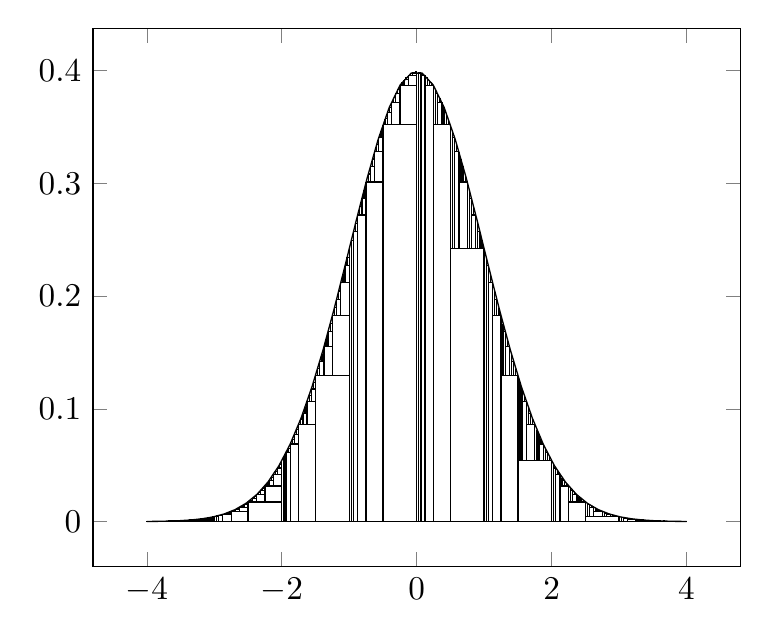
\begin{tikzpicture}[scale=1.2]
\begin{axis}
\addplot[domain=-4:4,samples=50] {e^(-x^2/2)/sqrt(2*pi)};
\draw (axis cs: -4, 0) -- (axis cs: 4, 0);
\draw (axis cs: -4, 0) -- (axis cs: -4, 1.3383022577439575E-4);
\draw (axis cs: -3, 0) -- (axis cs: -3, 1.3383022577439575E-4);
\draw (axis cs: -4, 0) -- (axis cs: -4, 1.338302257719816E-4);
\draw (axis cs: -7/2, 0) -- (axis cs: -7/2, 1.338302257719816E-4);
\draw (axis cs: -7/2, 0) -- (axis cs: -7/2, 8.726826968250417E-4);
\draw (axis cs: -3, 0) -- (axis cs: -3, 8.726826968250417E-4);
\draw (axis cs: -7/2, 8.726826968250417E-4) -- (axis cs: -3, 8.726826968250417E-4);
\draw (axis cs: -4, 0) -- (axis cs: -4, 1.3383022577495704E-4);
\draw (axis cs: -15/4, 0) -- (axis cs: -15/4, 1.3383022577495704E-4);
\draw (axis cs: -15/4, 0) -- (axis cs: -15/4, 3.525956827459561E-4);
\draw (axis cs: -7/2, 0) -- (axis cs: -7/2, 3.525956827459561E-4);
\draw (axis cs: -15/4, 3.525956827459561E-4) -- (axis cs: -7/2, 3.525956827459561E-4);
\draw (axis cs: -7/2, 8.726826968250417E-4) -- (axis cs: -7/2, 8.726826977454657E-4);
\draw (axis cs: -13/4, 8.726826968250417E-4) -- (axis cs: -13/4, 8.726826977454657E-4);
\draw (axis cs: -13/4, 8.726826968250417E-4) -- (axis cs: -13/4, 0.002029048066730719);
\draw (axis cs: -3, 8.726826968250417E-4) -- (axis cs: -3, 0.002029048066730719);
\draw (axis cs: -13/4, 0.002029048066730719) -- (axis cs: -3, 0.002029048066730719);
\draw (axis cs: -4, 0) -- (axis cs: -4, 1.338302257727162E-4);
\draw (axis cs: -31/8, 0) -- (axis cs: -31/8, 1.338302257727162E-4);
\draw (axis cs: -31/8, 0) -- (axis cs: -31/8, 2.189316378817986E-4);
\draw (axis cs: -15/4, 0) -- (axis cs: -15/4, 2.189316378817986E-4);
\draw (axis cs: -31/8, 2.189316378817986E-4) -- (axis cs: -15/4, 2.189316378817986E-4);
\draw (axis cs: -15/4, 3.525956827459561E-4) -- (axis cs: -15/4, 3.5259568295179194E-4);
\draw (axis cs: -29/8, 3.525956827459561E-4) -- (axis cs: -29/8, 3.5259568295179194E-4);
\draw (axis cs: -29/8, 3.525956827459561E-4) -- (axis cs: -29/8, 5.590615236813285E-4);
\draw (axis cs: -7/2, 3.525956827459561E-4) -- (axis cs: -7/2, 5.590615236813285E-4);
\draw (axis cs: -29/8, 5.590615236813285E-4) -- (axis cs: -7/2, 5.590615236813285E-4);
\draw (axis cs: -7/2, 8.726826968250417E-4) -- (axis cs: -7/2, 8.726826970219815E-4);
\draw (axis cs: -27/8, 8.726826968250417E-4) -- (axis cs: -27/8, 8.726826970219815E-4);
\draw (axis cs: -27/8, 8.726826968250417E-4) -- (axis cs: -27/8, 0.0013411188787273267);
\draw (axis cs: -13/4, 8.726826968250417E-4) -- (axis cs: -13/4, 0.0013411188787273267);
\draw (axis cs: -27/8, 0.0013411188787273267) -- (axis cs: -13/4, 0.0013411188787273267);
\draw (axis cs: -13/4, 0.002029048066730719) -- (axis cs: -13/4, 0.0020290480646332917);
\draw (axis cs: -25/8, 0.002029048066730719) -- (axis cs: -25/8, 0.0020290480646332917);
\draw (axis cs: -25/8, 0.002029048066730719) -- (axis cs: -25/8, 0.0030222580445213106);
\draw (axis cs: -3, 0.002029048066730719) -- (axis cs: -3, 0.0030222580445213106);
\draw (axis cs: -25/8, 0.0030222580445213106) -- (axis cs: -3, 0.0030222580445213106);
\draw (axis cs: -4, 0) -- (axis cs: -4, 1.338302257755516E-4);
\draw (axis cs: -63/16, 0) -- (axis cs: -63/16, 1.338302257755516E-4);
\draw (axis cs: -63/16, 0) -- (axis cs: -63/16, 1.7150611128694776E-4);
\draw (axis cs: -31/8, 0) -- (axis cs: -31/8, 1.7150611128694776E-4);
\draw (axis cs: -63/16, 1.7150611128694776E-4) -- (axis cs: -31/8, 1.7150611128694776E-4);
\draw (axis cs: -31/8, 2.189316378817986E-4) -- (axis cs: -31/8, 2.1893163795207372E-4);
\draw (axis cs: -61/16, 2.189316378817986E-4) -- (axis cs: -61/16, 2.1893163795207372E-4);
\draw (axis cs: -61/16, 2.189316378817986E-4) -- (axis cs: -61/16, 2.783818969778259E-4);
\draw (axis cs: -15/4, 2.189316378817986E-4) -- (axis cs: -15/4, 2.783818969778259E-4);
\draw (axis cs: -61/16, 2.783818969778259E-4) -- (axis cs: -15/4, 2.783818969778259E-4);
\draw (axis cs: -15/4, 3.525956827459561E-4) -- (axis cs: -15/4, 3.525956827885839E-4);
\draw (axis cs: -59/16, 3.525956827459561E-4) -- (axis cs: -59/16, 3.525956827885839E-4);
\draw (axis cs: -59/16, 3.525956827459561E-4) -- (axis cs: -59/16, 4.4485300506178784E-4);
\draw (axis cs: -29/8, 3.525956827459561E-4) -- (axis cs: -29/8, 4.4485300506178784E-4);
\draw (axis cs: -59/16, 4.4485300506178784E-4) -- (axis cs: -29/8, 4.4485300506178784E-4);
\draw (axis cs: -29/8, 5.590615236813285E-4) -- (axis cs: -29/8, 5.590615233489036E-4);
\draw (axis cs: -57/16, 5.590615236813285E-4) -- (axis cs: -57/16, 5.590615233489036E-4);
\draw (axis cs: -57/16, 5.590615236813285E-4) -- (axis cs: -57/16, 6.99852012164985E-4);
\draw (axis cs: -7/2, 5.590615236813285E-4) -- (axis cs: -7/2, 6.99852012164985E-4);
\draw (axis cs: -57/16, 6.99852012164985E-4) -- (axis cs: -7/2, 6.99852012164985E-4);
\draw (axis cs: -7/2, 8.726826968250417E-4) -- (axis cs: -7/2, 8.726826979047949E-4);
\draw (axis cs: -55/16, 8.726826968250417E-4) -- (axis cs: -55/16, 8.726826979047949E-4);
\draw (axis cs: -55/16, 8.726826968250417E-4) -- (axis cs: -55/16, 0.0010839520026024215);
\draw (axis cs: -27/8, 8.726826968250417E-4) -- (axis cs: -27/8, 0.0010839520026024215);
\draw (axis cs: -55/16, 0.0010839520026024215) -- (axis cs: -27/8, 0.0010839520026024215);
\draw (axis cs: -27/8, 0.0013411188787273267) -- (axis cs: -27/8, 0.0013411188774714465);
\draw (axis cs: -53/16, 0.0013411188787273267) -- (axis cs: -53/16, 0.0013411188774714465);
\draw (axis cs: -53/16, 0.0013411188787273267) -- (axis cs: -53/16, 0.0016528294268795848);
\draw (axis cs: -13/4, 0.0013411188787273267) -- (axis cs: -13/4, 0.0016528294268795848);
\draw (axis cs: -53/16, 0.0016528294268795848) -- (axis cs: -13/4, 0.0016528294268795848);
\draw (axis cs: -13/4, 0.002029048066730719) -- (axis cs: -13/4, 0.002029048067287304);
\draw (axis cs: -51/16, 0.002029048066730719) -- (axis cs: -51/16, 0.002029048067287304);
\draw (axis cs: -51/16, 0.002029048066730719) -- (axis cs: -51/16, 0.00248119084808154);
\draw (axis cs: -25/8, 0.002029048066730719) -- (axis cs: -25/8, 0.00248119084808154);
\draw (axis cs: -51/16, 0.00248119084808154) -- (axis cs: -25/8, 0.00248119084808154);
\draw (axis cs: -25/8, 0.0030222580445213106) -- (axis cs: -25/8, 0.003022258049502977);
\draw (axis cs: -49/16, 0.0030222580445213106) -- (axis cs: -49/16, 0.003022258049502977);
\draw (axis cs: -49/16, 0.0030222580445213106) -- (axis cs: -49/16, 0.0036669623631740054);
\draw (axis cs: -3, 0.0030222580445213106) -- (axis cs: -3, 0.0036669623631740054);
\draw (axis cs: -49/16, 0.0036669623631740054) -- (axis cs: -3, 0.0036669623631740054);
\draw (axis cs: -4, 0) -- (axis cs: -4, 1.3383022577349429E-4);
\draw (axis cs: -127/32, 0) -- (axis cs: -127/32, 1.3383022577349429E-4);
\draw (axis cs: -127/32, 0) -- (axis cs: -127/32, 1.5157548380131383E-4);
\draw (axis cs: -63/16, 0) -- (axis cs: -63/16, 1.5157548380131383E-4);
\draw (axis cs: -127/32, 1.5157548380131383E-4) -- (axis cs: -63/16, 1.5157548380131383E-4);
\draw (axis cs: -63/16, 1.7150611128694776E-4) -- (axis cs: -63/16, 1.7150611126648675E-4);
\draw (axis cs: -125/32, 1.7150611128694776E-4) -- (axis cs: -125/32, 1.7150611126648675E-4);
\draw (axis cs: -125/32, 1.7150611128694776E-4) -- (axis cs: -125/32, 1.938679959484055E-4);
\draw (axis cs: -31/8, 1.7150611128694776E-4) -- (axis cs: -31/8, 1.938679959484055E-4);
\draw (axis cs: -125/32, 1.938679959484055E-4) -- (axis cs: -31/8, 1.938679959484055E-4);
\draw (axis cs: -31/8, 2.189316378817986E-4) -- (axis cs: -31/8, 2.1893163789547392E-4);
\draw (axis cs: -123/32, 2.189316378817986E-4) -- (axis cs: -123/32, 2.1893163789547392E-4);
\draw (axis cs: -123/32, 2.189316378817986E-4) -- (axis cs: -123/32, 2.4699423459166776E-4);
\draw (axis cs: -61/16, 2.189316378817986E-4) -- (axis cs: -61/16, 2.4699423459166776E-4);
\draw (axis cs: -123/32, 2.4699423459166776E-4) -- (axis cs: -61/16, 2.4699423459166776E-4);
\draw (axis cs: -61/16, 2.783818969778259E-4) -- (axis cs: -61/16, 2.783818968854738E-4);
\draw (axis cs: -121/32, 2.783818969778259E-4) -- (axis cs: -121/32, 2.783818968854738E-4);
\draw (axis cs: -121/32, 2.783818969778259E-4) -- (axis cs: -121/32, 3.134520019157421E-4);
\draw (axis cs: -15/4, 2.783818969778259E-4) -- (axis cs: -15/4, 3.134520019157421E-4);
\draw (axis cs: -121/32, 3.134520019157421E-4) -- (axis cs: -15/4, 3.134520019157421E-4);
\draw (axis cs: -15/4, 3.525956827459561E-4) -- (axis cs: -15/4, 3.525956829862783E-4);
\draw (axis cs: -119/32, 3.525956827459561E-4) -- (axis cs: -119/32, 3.525956829862783E-4);
\draw (axis cs: -119/32, 3.525956827459561E-4) -- (axis cs: -119/32, 3.962404584351427E-4);
\draw (axis cs: -59/16, 3.525956827459561E-4) -- (axis cs: -59/16, 3.962404584351427E-4);
\draw (axis cs: -119/32, 3.962404584351427E-4) -- (axis cs: -59/16, 3.962404584351427E-4);
\draw (axis cs: -59/16, 4.4485300506178784E-4) -- (axis cs: -59/16, 4.4485300482601024E-4);
\draw (axis cs: -117/32, 4.4485300506178784E-4) -- (axis cs: -117/32, 4.4485300482601024E-4);
\draw (axis cs: -117/32, 4.4485300506178784E-4) -- (axis cs: -117/32, 4.989420690804763E-4);
\draw (axis cs: -29/8, 4.4485300506178784E-4) -- (axis cs: -29/8, 4.989420690804763E-4);
\draw (axis cs: -117/32, 4.989420690804763E-4) -- (axis cs: -29/8, 4.989420690804763E-4);
\draw (axis cs: -29/8, 5.590615236813285E-4) -- (axis cs: -29/8, 5.590615237668537E-4);
\draw (axis cs: -115/32, 5.590615236813285E-4) -- (axis cs: -115/32, 5.590615237668537E-4);
\draw (axis cs: -115/32, 5.590615236813285E-4) -- (axis cs: -115/32, 6.258135581015341E-4);
\draw (axis cs: -57/16, 5.590615236813285E-4) -- (axis cs: -57/16, 6.258135581015341E-4);
\draw (axis cs: -115/32, 6.258135581015341E-4) -- (axis cs: -57/16, 6.258135581015341E-4);
\draw (axis cs: -57/16, 6.99852012164985E-4) -- (axis cs: -57/16, 6.998520128349937E-4);
\draw (axis cs: -113/32, 6.99852012164985E-4) -- (axis cs: -113/32, 6.998520128349937E-4);
\draw (axis cs: -113/32, 6.99852012164985E-4) -- (axis cs: -113/32, 7.818858407131201E-4);
\draw (axis cs: -7/2, 6.99852012164985E-4) -- (axis cs: -7/2, 7.818858407131201E-4);
\draw (axis cs: -113/32, 7.818858407131201E-4) -- (axis cs: -7/2, 7.818858407131201E-4);
\draw (axis cs: -7/2, 8.726826968250417E-4) -- (axis cs: -7/2, 8.726826972305451E-4);
\draw (axis cs: -111/32, 8.726826968250417E-4) -- (axis cs: -111/32, 8.726826972305451E-4);
\draw (axis cs: -111/32, 8.726826968250417E-4) -- (axis cs: -111/32, 9.730726504887151E-4);
\draw (axis cs: -55/16, 8.726826968250417E-4) -- (axis cs: -55/16, 9.730726504887151E-4);
\draw (axis cs: -111/32, 9.730726504887151E-4) -- (axis cs: -55/16, 9.730726504887151E-4);
\draw (axis cs: -55/16, 0.0010839520026024215) -- (axis cs: -55/16, 0.0010839520015470169);
\draw (axis cs: -109/32, 0.0010839520026024215) -- (axis cs: -109/32, 0.0010839520015470169);
\draw (axis cs: -109/32, 0.0010839520026024215) -- (axis cs: -109/32, 0.0012062872049105834);
\draw (axis cs: -27/8, 0.0010839520026024215) -- (axis cs: -27/8, 0.0012062872049105834);
\draw (axis cs: -109/32, 0.0012062872049105834) -- (axis cs: -27/8, 0.0012062872049105834);
\draw (axis cs: -27/8, 0.0013411188787273267) -- (axis cs: -27/8, 0.0013411188790363948);
\draw (axis cs: -107/32, 0.0013411188787273267) -- (axis cs: -107/32, 0.0013411188790363948);
\draw (axis cs: -107/32, 0.0013411188787273267) -- (axis cs: -107/32, 0.0014895658752694212);
\draw (axis cs: -53/16, 0.0013411188787273267) -- (axis cs: -53/16, 0.0014895658752694212);
\draw (axis cs: -107/32, 0.0014895658752694212) -- (axis cs: -53/16, 0.0014895658752694212);
\draw (axis cs: -53/16, 0.0016528294268795848) -- (axis cs: -53/16, 0.001652829429114738);
\draw (axis cs: -105/32, 0.0016528294268795848) -- (axis cs: -105/32, 0.001652829429114738);
\draw (axis cs: -105/32, 0.0016528294268795848) -- (axis cs: -105/32, 0.0018321973212320946);
\draw (axis cs: -13/4, 0.0016528294268795848) -- (axis cs: -13/4, 0.0018321973212320946);
\draw (axis cs: -105/32, 0.0018321973212320946) -- (axis cs: -13/4, 0.0018321973212320946);
\draw (axis cs: -13/4, 0.002029048066730719) -- (axis cs: -13/4, 0.002029048065361871);
\draw (axis cs: -103/32, 0.002029048066730719) -- (axis cs: -103/32, 0.002029048065361871);
\draw (axis cs: -103/32, 0.002029048066730719) -- (axis cs: -103/32, 0.002244855083569142);
\draw (axis cs: -51/16, 0.002029048066730719) -- (axis cs: -51/16, 0.002244855083569142);
\draw (axis cs: -103/32, 0.002244855083569142) -- (axis cs: -51/16, 0.002244855083569142);
\draw (axis cs: -51/16, 0.00248119084808154) -- (axis cs: -51/16, 0.0024811908452780345);
\draw (axis cs: -101/32, 0.00248119084808154) -- (axis cs: -101/32, 0.0024811908452780345);
\draw (axis cs: -101/32, 0.00248119084808154) -- (axis cs: -101/32, 0.0027397309388828904);
\draw (axis cs: -25/8, 0.00248119084808154) -- (axis cs: -25/8, 0.0027397309388828904);
\draw (axis cs: -101/32, 0.0027397309388828904) -- (axis cs: -25/8, 0.0027397309388828904);
\draw (axis cs: -25/8, 0.0030222580445213106) -- (axis cs: -25/8, 0.0030222580455647884);
\draw (axis cs: -99/32, 0.0030222580445213106) -- (axis cs: -99/32, 0.0030222580455647884);
\draw (axis cs: -99/32, 0.0030222580445213106) -- (axis cs: -99/32, 0.0033306657796143787);
\draw (axis cs: -49/16, 0.0030222580445213106) -- (axis cs: -49/16, 0.0033306657796143787);
\draw (axis cs: -99/32, 0.0033306657796143787) -- (axis cs: -49/16, 0.0033306657796143787);
\draw (axis cs: -49/16, 0.0036669623631740054) -- (axis cs: -49/16, 0.0036669623579181037);
\draw (axis cs: -97/32, 0.0036669623631740054) -- (axis cs: -97/32, 0.0036669623579181037);
\draw (axis cs: -97/32, 0.0036669623631740054) -- (axis cs: -97/32, 0.0040332740584328826);
\draw (axis cs: -3, 0.0036669623631740054) -- (axis cs: -3, 0.0040332740584328826);
\draw (axis cs: -97/32, 0.0040332740584328826) -- (axis cs: -3, 0.0040332740584328826);
\draw (axis cs: -3, 0) -- (axis cs: -3, 0.004431848412174211);
\draw (axis cs: -2, 0) -- (axis cs: -2, 0.004431848412174211);
\draw (axis cs: -3, 0) -- (axis cs: -3, 0.0044318484121142546);
\draw (axis cs: -5/2, 0) -- (axis cs: -5/2, 0.0044318484121142546);
\draw (axis cs: -5/2, 0) -- (axis cs: -5/2, 0.017528300519095555);
\draw (axis cs: -2, 0) -- (axis cs: -2, 0.017528300519095555);
\draw (axis cs: -5/2, 0.017528300519095555) -- (axis cs: -2, 0.017528300519095555);
\draw (axis cs: -3, 0) -- (axis cs: -3, 0.004431848412188154);
\draw (axis cs: -11/4, 0) -- (axis cs: -11/4, 0.004431848412188154);
\draw (axis cs: -11/4, 0) -- (axis cs: -11/4, 0.009093562508749794);
\draw (axis cs: -5/2, 0) -- (axis cs: -5/2, 0.009093562508749794);
\draw (axis cs: -11/4, 0.009093562508749794) -- (axis cs: -5/2, 0.009093562508749794);
\draw (axis cs: -5/2, 0.017528300519095555) -- (axis cs: -5/2, 0.017528300532300707);
\draw (axis cs: -9/4, 0.017528300519095555) -- (axis cs: -9/4, 0.017528300532300707);
\draw (axis cs: -9/4, 0.017528300519095555) -- (axis cs: -9/4, 0.031739651937800026);
\draw (axis cs: -2, 0.017528300519095555) -- (axis cs: -2, 0.031739651937800026);
\draw (axis cs: -9/4, 0.031739651937800026) -- (axis cs: -2, 0.031739651937800026);
\draw (axis cs: -3, 0) -- (axis cs: -3, 0.004431848412132499);
\draw (axis cs: -23/8, 0) -- (axis cs: -23/8, 0.004431848412132499);
\draw (axis cs: -23/8, 0) -- (axis cs: -23/8, 0.006398120313264456);
\draw (axis cs: -11/4, 0) -- (axis cs: -11/4, 0.006398120313264456);
\draw (axis cs: -23/8, 0.006398120313264456) -- (axis cs: -11/4, 0.006398120313264456);
\draw (axis cs: -11/4, 0.009093562508749794) -- (axis cs: -11/4, 0.00909356251264275);
\draw (axis cs: -21/8, 0.009093562508749794) -- (axis cs: -21/8, 0.00909356251264275);
\draw (axis cs: -21/8, 0.009093562508749794) -- (axis cs: -21/8, 0.012724181620715534);
\draw (axis cs: -5/2, 0.009093562508749794) -- (axis cs: -5/2, 0.012724181620715534);
\draw (axis cs: -21/8, 0.012724181620715534) -- (axis cs: -5/2, 0.012724181620715534);
\draw (axis cs: -5/2, 0.017528300519095555) -- (axis cs: -5/2, 0.017528300521921024);
\draw (axis cs: -19/8, 0.017528300519095555) -- (axis cs: -19/8, 0.017528300521921024);
\draw (axis cs: -19/8, 0.017528300519095555) -- (axis cs: -19/8, 0.023771900895236606);
\draw (axis cs: -9/4, 0.017528300519095555) -- (axis cs: -9/4, 0.023771900895236606);
\draw (axis cs: -19/8, 0.023771900895236606) -- (axis cs: -9/4, 0.023771900895236606);
\draw (axis cs: -9/4, 0.031739651937800026) -- (axis cs: -9/4, 0.03173965191508592);
\draw (axis cs: -17/8, 0.031739651937800026) -- (axis cs: -17/8, 0.03173965191508592);
\draw (axis cs: -17/8, 0.031739651937800026) -- (axis cs: -17/8, 0.04172098534385047);
\draw (axis cs: -2, 0.031739651937800026) -- (axis cs: -2, 0.04172098534385047);
\draw (axis cs: -17/8, 0.04172098534385047) -- (axis cs: -2, 0.04172098534385047);
\draw (axis cs: -3, 0) -- (axis cs: -3, 0.004431848412202919);
\draw (axis cs: -47/16, 0) -- (axis cs: -47/16, 0.004431848412202919);
\draw (axis cs: -47/16, 0) -- (axis cs: -47/16, 0.005335398733726687);
\draw (axis cs: -23/8, 0) -- (axis cs: -23/8, 0.005335398733726687);
\draw (axis cs: -47/16, 0.005335398733726687) -- (axis cs: -23/8, 0.005335398733726687);
\draw (axis cs: -23/8, 0.006398120313264456) -- (axis cs: -23/8, 0.006398120314788203);
\draw (axis cs: -45/16, 0.006398120313264456) -- (axis cs: -45/16, 0.006398120314788203);
\draw (axis cs: -45/16, 0.006398120313264456) -- (axis cs: -45/16, 0.007642605826431574);
\draw (axis cs: -11/4, 0.006398120313264456) -- (axis cs: -11/4, 0.007642605826431574);
\draw (axis cs: -45/16, 0.007642605826431574) -- (axis cs: -11/4, 0.007642605826431574);
\draw (axis cs: -11/4, 0.009093562508749794) -- (axis cs: -11/4, 0.009093562509556006);
\draw (axis cs: -43/16, 0.009093562508749794) -- (axis cs: -43/16, 0.009093562509556006);
\draw (axis cs: -43/16, 0.009093562508749794) -- (axis cs: -43/16, 0.010777801717027505);
\draw (axis cs: -21/8, 0.009093562508749794) -- (axis cs: -21/8, 0.010777801717027505);
\draw (axis cs: -43/16, 0.010777801717027505) -- (axis cs: -21/8, 0.010777801717027505);
\draw (axis cs: -21/8, 0.012724181620715534) -- (axis cs: -21/8, 0.01272418161523674);
\draw (axis cs: -41/16, 0.012724181620715534) -- (axis cs: -41/16, 0.01272418161523674);
\draw (axis cs: -41/16, 0.012724181620715534) -- (axis cs: -41/16, 0.014963495804646555);
\draw (axis cs: -5/2, 0.012724181620715534) -- (axis cs: -5/2, 0.014963495804646555);
\draw (axis cs: -41/16, 0.014963495804646555) -- (axis cs: -5/2, 0.014963495804646555);
\draw (axis cs: -5/2, 0.017528300519095555) -- (axis cs: -5/2, 0.01752830053458658);
\draw (axis cs: -39/16, 0.017528300519095555) -- (axis cs: -39/16, 0.01752830053458658);
\draw (axis cs: -39/16, 0.017528300519095555) -- (axis cs: -39/16, 0.02045267381944624);
\draw (axis cs: -19/8, 0.017528300519095555) -- (axis cs: -19/8, 0.02045267381944624);
\draw (axis cs: -39/16, 0.02045267381944624) -- (axis cs: -19/8, 0.02045267381944624);
\draw (axis cs: -19/8, 0.023771900895236606) -- (axis cs: -19/8, 0.023771900879571463);
\draw (axis cs: -37/16, 0.023771900895236606) -- (axis cs: -37/16, 0.023771900879571463);
\draw (axis cs: -37/16, 0.023771900895236606) -- (axis cs: -37/16, 0.02752208085490523);
\draw (axis cs: -9/4, 0.023771900895236606) -- (axis cs: -9/4, 0.02752208085490523);
\draw (axis cs: -37/16, 0.02752208085490523) -- (axis cs: -9/4, 0.02752208085490523);
\draw (axis cs: -9/4, 0.031739651937800026) -- (axis cs: -9/4, 0.031739651943827586);
\draw (axis cs: -35/16, 0.031739651937800026) -- (axis cs: -35/16, 0.031739651943827586);
\draw (axis cs: -35/16, 0.031739651937800026) -- (axis cs: -35/16, 0.03646083329698946);
\draw (axis cs: -17/8, 0.031739651937800026) -- (axis cs: -17/8, 0.03646083329698946);
\draw (axis cs: -35/16, 0.03646083329698946) -- (axis cs: -17/8, 0.03646083329698946);
\draw (axis cs: -17/8, 0.04172098534385047) -- (axis cs: -17/8, 0.04172098539061392);
\draw (axis cs: -33/16, 0.04172098534385047) -- (axis cs: -33/16, 0.04172098539061392);
\draw (axis cs: -33/16, 0.04172098534385047) -- (axis cs: -33/16, 0.0475538914080623);
\draw (axis cs: -2, 0.04172098534385047) -- (axis cs: -2, 0.0475538914080623);
\draw (axis cs: -33/16, 0.0475538914080623) -- (axis cs: -2, 0.0475538914080623);
\draw (axis cs: -3, 0) -- (axis cs: -3, 0.004431848412151822);
\draw (axis cs: -95/32, 0) -- (axis cs: -95/32, 0.004431848412151822);
\draw (axis cs: -95/32, 0) -- (axis cs: -95/32, 0.004865057159669394);
\draw (axis cs: -47/16, 0) -- (axis cs: -47/16, 0.004865057159669394);
\draw (axis cs: -95/32, 0.004865057159669394) -- (axis cs: -47/16, 0.004865057159669394);
\draw (axis cs: -47/16, 0.005335398733726687) -- (axis cs: -47/16, 0.005335398733251823);
\draw (axis cs: -93/32, 0.005335398733726687) -- (axis cs: -93/32, 0.005335398733251823);
\draw (axis cs: -93/32, 0.005335398733726687) -- (axis cs: -93/32, 0.005845500471043691);
\draw (axis cs: -23/8, 0.005335398733726687) -- (axis cs: -23/8, 0.005845500471043691);
\draw (axis cs: -93/32, 0.005845500471043691) -- (axis cs: -23/8, 0.005845500471043691);
\draw (axis cs: -23/8, 0.006398120313264456) -- (axis cs: -23/8, 0.0063981203135609725);
\draw (axis cs: -91/32, 0.006398120313264456) -- (axis cs: -91/32, 0.0063981203135609725);
\draw (axis cs: -91/32, 0.006398120313264456) -- (axis cs: -91/32, 0.006996148024288882);
\draw (axis cs: -45/16, 0.006398120313264456) -- (axis cs: -45/16, 0.006996148024288882);
\draw (axis cs: -91/32, 0.006996148024288882) -- (axis cs: -45/16, 0.006996148024288882);
\draw (axis cs: -45/16, 0.007642605826431574) -- (axis cs: -45/16, 0.007642605824561196);
\draw (axis cs: -89/32, 0.007642605826431574) -- (axis cs: -89/32, 0.007642605824561196);
\draw (axis cs: -89/32, 0.007642605826431574) -- (axis cs: -89/32, 0.008340648450385625);
\draw (axis cs: -11/4, 0.007642605826431574) -- (axis cs: -11/4, 0.008340648450385625);
\draw (axis cs: -89/32, 0.008340648450385625) -- (axis cs: -11/4, 0.008340648450385625);
\draw (axis cs: -11/4, 0.009093562508749794) -- (axis cs: -11/4, 0.009093562513294988);
\draw (axis cs: -87/32, 0.009093562508749794) -- (axis cs: -87/32, 0.009093562513294988);
\draw (axis cs: -87/32, 0.009093562508749794) -- (axis cs: -87/32, 0.009904765112088453);
\draw (axis cs: -43/16, 0.009093562508749794) -- (axis cs: -43/16, 0.009904765112088453);
\draw (axis cs: -87/32, 0.009904765112088453) -- (axis cs: -43/16, 0.009904765112088453);
\draw (axis cs: -43/16, 0.010777801717027505) -- (axis cs: -43/16, 0.010777801712864257);
\draw (axis cs: -85/32, 0.010777801717027505) -- (axis cs: -85/32, 0.010777801712864257);
\draw (axis cs: -85/32, 0.010777801717027505) -- (axis cs: -85/32, 0.011716343127226523);
\draw (axis cs: -21/8, 0.010777801717027505) -- (axis cs: -21/8, 0.011716343127226523);
\draw (axis cs: -85/32, 0.011716343127226523) -- (axis cs: -21/8, 0.011716343127226523);
\draw (axis cs: -21/8, 0.012724181620715534) -- (axis cs: -21/8, 0.012724181622125099);
\draw (axis cs: -83/32, 0.012724181620715534) -- (axis cs: -83/32, 0.012724181622125099);
\draw (axis cs: -83/32, 0.012724181620715534) -- (axis cs: -83/32, 0.013805226005016956);
\draw (axis cs: -41/16, 0.012724181620715534) -- (axis cs: -41/16, 0.013805226005016956);
\draw (axis cs: -83/32, 0.013805226005016956) -- (axis cs: -41/16, 0.013805226005016956);
\draw (axis cs: -41/16, 0.014963495804646555) -- (axis cs: -41/16, 0.014963495814950807);
\draw (axis cs: -81/32, 0.014963495804646555) -- (axis cs: -81/32, 0.014963495814950807);
\draw (axis cs: -81/32, 0.014963495804646555) -- (axis cs: -81/32, 0.016203114331012073);
\draw (axis cs: -5/2, 0.014963495804646555) -- (axis cs: -5/2, 0.016203114331012073);
\draw (axis cs: -81/32, 0.016203114331012073) -- (axis cs: -5/2, 0.016203114331012073);
\draw (axis cs: -5/2, 0.017528300519095555) -- (axis cs: -5/2, 0.017528300524913245);
\draw (axis cs: -79/32, 0.017528300519095555) -- (axis cs: -79/32, 0.017528300524913245);
\draw (axis cs: -79/32, 0.017528300519095555) -- (axis cs: -79/32, 0.018943359845972896);
\draw (axis cs: -39/16, 0.017528300519095555) -- (axis cs: -39/16, 0.018943359845972896);
\draw (axis cs: -79/32, 0.018943359845972896) -- (axis cs: -39/16, 0.018943359845972896);
\draw (axis cs: -39/16, 0.02045267381944624) -- (axis cs: -39/16, 0.020452673805325384);
\draw (axis cs: -77/32, 0.02045267381944624) -- (axis cs: -77/32, 0.020452673805325384);
\draw (axis cs: -77/32, 0.02045267381944624) -- (axis cs: -77/32, 0.022060688331219873);
\draw (axis cs: -19/8, 0.02045267381944624) -- (axis cs: -19/8, 0.022060688331219873);
\draw (axis cs: -77/32, 0.022060688331219873) -- (axis cs: -19/8, 0.022060688331219873);
\draw (axis cs: -19/8, 0.023771900895236606) -- (axis cs: -19/8, 0.02377190089909175);
\draw (axis cs: -75/32, 0.023771900895236606) -- (axis cs: -75/32, 0.02377190089909175);
\draw (axis cs: -75/32, 0.023771900895236606) -- (axis cs: -75/32, 0.025590846204343713);
\draw (axis cs: -37/16, 0.023771900895236606) -- (axis cs: -37/16, 0.025590846204343713);
\draw (axis cs: -75/32, 0.025590846204343713) -- (axis cs: -37/16, 0.025590846204343713);
\draw (axis cs: -37/16, 0.02752208085490523) -- (axis cs: -37/16, 0.027522080880888054);
\draw (axis cs: -73/32, 0.02752208085490523) -- (axis cs: -73/32, 0.027522080880888054);
\draw (axis cs: -73/32, 0.02752208085490523) -- (axis cs: -73/32, 0.02957016658183054);
\draw (axis cs: -9/4, 0.02752208085490523) -- (axis cs: -9/4, 0.02957016658183054);
\draw (axis cs: -73/32, 0.02957016658183054) -- (axis cs: -9/4, 0.02957016658183054);
\draw (axis cs: -9/4, 0.031739651937800026) -- (axis cs: -9/4, 0.03173965192297608);
\draw (axis cs: -71/32, 0.031739651937800026) -- (axis cs: -71/32, 0.03173965192297608);
\draw (axis cs: -71/32, 0.031739651937800026) -- (axis cs: -71/32, 0.034035053103857585);
\draw (axis cs: -35/16, 0.031739651937800026) -- (axis cs: -35/16, 0.034035053103857585);
\draw (axis cs: -71/32, 0.034035053103857585) -- (axis cs: -35/16, 0.034035053103857585);
\draw (axis cs: -35/16, 0.03646083329698946) -- (axis cs: -35/16, 0.036460833268716866);
\draw (axis cs: -69/32, 0.03646083329698946) -- (axis cs: -69/32, 0.036460833268716866);
\draw (axis cs: -69/32, 0.03646083329698946) -- (axis cs: -69/32, 0.03902138062095352);
\draw (axis cs: -17/8, 0.03646083329698946) -- (axis cs: -17/8, 0.03902138062095352);
\draw (axis cs: -69/32, 0.03902138062095352) -- (axis cs: -17/8, 0.03902138062095352);
\draw (axis cs: -17/8, 0.04172098534385047) -- (axis cs: -17/8, 0.04172098535364571);
\draw (axis cs: -67/32, 0.04172098534385047) -- (axis cs: -67/32, 0.04172098535364571);
\draw (axis cs: -67/32, 0.04172098534385047) -- (axis cs: -67/32, 0.044563815441383485);
\draw (axis cs: -33/16, 0.04172098534385047) -- (axis cs: -33/16, 0.044563815441383485);
\draw (axis cs: -67/32, 0.044563815441383485) -- (axis cs: -33/16, 0.044563815441383485);
\draw (axis cs: -33/16, 0.0475538914080623) -- (axis cs: -33/16, 0.047553891362158915);
\draw (axis cs: -65/32, 0.0475538914080623) -- (axis cs: -65/32, 0.047553891362158915);
\draw (axis cs: -65/32, 0.0475538914080623) -- (axis cs: -65/32, 0.05069505982834406);
\draw (axis cs: -2, 0.0475538914080623) -- (axis cs: -2, 0.05069505982834406);
\draw (axis cs: -65/32, 0.05069505982834406) -- (axis cs: -2, 0.05069505982834406);
\draw (axis cs: -2, 0) -- (axis cs: -2, 0.05399096651510647);
\draw (axis cs: -1, 0) -- (axis cs: -1, 0.05399096651510647);
\draw (axis cs: -2, 0) -- (axis cs: -2, 0.05399096651461945);
\draw (axis cs: -3/2, 0) -- (axis cs: -3/2, 0.05399096651461945);
\draw (axis cs: -3/2, 0) -- (axis cs: -3/2, 0.1295175957790641);
\draw (axis cs: -1, 0) -- (axis cs: -1, 0.1295175957790641);
\draw (axis cs: -3/2, 0.1295175957790641) -- (axis cs: -1, 0.1295175957790641);
\draw (axis cs: -2, 0) -- (axis cs: -2, 0.05399096651521968);
\draw (axis cs: -7/4, 0) -- (axis cs: -7/4, 0.05399096651521968);
\draw (axis cs: -7/4, 0) -- (axis cs: -7/4, 0.08627731886973354);
\draw (axis cs: -3/2, 0) -- (axis cs: -3/2, 0.08627731886973354);
\draw (axis cs: -7/4, 0.08627731886973354) -- (axis cs: -3/2, 0.08627731886973354);
\draw (axis cs: -3/2, 0.1295175957790641) -- (axis cs: -3/2, 0.12951759583760825);
\draw (axis cs: -5/4, 0.1295175957790641) -- (axis cs: -5/4, 0.12951759583760825);
\draw (axis cs: -5/4, 0.1295175957790641) -- (axis cs: -5/4, 0.18264908571553998);
\draw (axis cs: -1, 0.1295175957790641) -- (axis cs: -1, 0.18264908571553998);
\draw (axis cs: -5/4, 0.18264908571553998) -- (axis cs: -1, 0.18264908571553998);
\draw (axis cs: -2, 0) -- (axis cs: -2, 0.05399096651476765);
\draw (axis cs: -15/8, 0) -- (axis cs: -15/8, 0.05399096651476765);
\draw (axis cs: -15/8, 0) -- (axis cs: -15/8, 0.06878627584450751);
\draw (axis cs: -7/4, 0) -- (axis cs: -7/4, 0.06878627584450751);
\draw (axis cs: -15/8, 0.06878627584450751) -- (axis cs: -7/4, 0.06878627584450751);
\draw (axis cs: -7/4, 0.08627731886973354) -- (axis cs: -7/4, 0.08627731889323777);
\draw (axis cs: -13/8, 0.08627731886973354) -- (axis cs: -13/8, 0.08627731889323777);
\draw (axis cs: -13/8, 0.08627731886973354) -- (axis cs: -13/8, 0.1065382682543817);
\draw (axis cs: -3/2, 0.08627731886973354) -- (axis cs: -3/2, 0.1065382682543817);
\draw (axis cs: -13/8, 0.1065382682543817) -- (axis cs: -3/2, 0.1065382682543817);
\draw (axis cs: -3/2, 0.1295175957790641) -- (axis cs: -3/2, 0.12951759579159058);
\draw (axis cs: -11/8, 0.1295175957790641) -- (axis cs: -11/8, 0.12951759579159058);
\draw (axis cs: -11/8, 0.1295175957790641) -- (axis cs: -11/8, 0.1550122657049006);
\draw (axis cs: -5/4, 0.1295175957790641) -- (axis cs: -5/4, 0.1550122657049006);
\draw (axis cs: -11/8, 0.1550122657049006) -- (axis cs: -5/4, 0.1550122657049006);
\draw (axis cs: -5/4, 0.18264908571553998) -- (axis cs: -5/4, 0.18264908564292295);
\draw (axis cs: -9/8, 0.18264908571553998) -- (axis cs: -9/8, 0.18264908564292295);
\draw (axis cs: -9/8, 0.18264908571553998) -- (axis cs: -9/8, 0.21187664601098163);
\draw (axis cs: -1, 0.18264908571553998) -- (axis cs: -1, 0.21187664601098163);
\draw (axis cs: -9/8, 0.21187664601098163) -- (axis cs: -1, 0.21187664601098163);
\draw (axis cs: -2, 0) -- (axis cs: -2, 0.053990966515339564);
\draw (axis cs: -31/16, 0) -- (axis cs: -31/16, 0.053990966515339564);
\draw (axis cs: -31/16, 0) -- (axis cs: -31/16, 0.06106040505722279);
\draw (axis cs: -15/8, 0) -- (axis cs: -15/8, 0.06106040505722279);
\draw (axis cs: -31/16, 0.06106040505722279) -- (axis cs: -15/8, 0.06106040505722279);
\draw (axis cs: -15/8, 0.06878627584450751) -- (axis cs: -15/8, 0.06878627585519127);
\draw (axis cs: -29/16, 0.06878627584450751) -- (axis cs: -29/16, 0.06878627585519127);
\draw (axis cs: -29/16, 0.06878627584450751) -- (axis cs: -29/16, 0.07718758448973091);
\draw (axis cs: -7/4, 0.06878627584450751) -- (axis cs: -7/4, 0.07718758448973091);
\draw (axis cs: -29/16, 0.07718758448973091) -- (axis cs: -7/4, 0.07718758448973091);
\draw (axis cs: -7/4, 0.08627731886973354) -- (axis cs: -7/4, 0.08627731887460113);
\draw (axis cs: -27/16, 0.08627731886973354) -- (axis cs: -27/16, 0.08627731887460113);
\draw (axis cs: -27/16, 0.08627731886973354) -- (axis cs: -27/16, 0.09606150099889124);
\draw (axis cs: -13/8, 0.08627731886973354) -- (axis cs: -13/8, 0.09606150099889124);
\draw (axis cs: -27/16, 0.09606150099889124) -- (axis cs: -13/8, 0.09606150099889124);
\draw (axis cs: -13/8, 0.1065382682543817) -- (axis cs: -13/8, 0.1065382682259839);
\draw (axis cs: -25/16, 0.1065382682543817) -- (axis cs: -25/16, 0.1065382682259839);
\draw (axis cs: -25/16, 0.1065382682543817) -- (axis cs: -25/16, 0.11769701131416355);
\draw (axis cs: -3/2, 0.1065382682543817) -- (axis cs: -3/2, 0.11769701131416355);
\draw (axis cs: -25/16, 0.11769701131416355) -- (axis cs: -3/2, 0.11769701131416355);
\draw (axis cs: -3/2, 0.1295175957790641) -- (axis cs: -3/2, 0.12951759584774244);
\draw (axis cs: -23/16, 0.1295175957790641) -- (axis cs: -23/16, 0.12951759584774244);
\draw (axis cs: -23/16, 0.1295175957790641) -- (axis cs: -23/16, 0.14196969539624416);
\draw (axis cs: -11/8, 0.1295175957790641) -- (axis cs: -11/8, 0.14196969539624416);
\draw (axis cs: -23/16, 0.14196969539624416) -- (axis cs: -11/8, 0.14196969539624416);
\draw (axis cs: -11/8, 0.1550122657049006) -- (axis cs: -11/8, 0.15501226564576137);
\draw (axis cs: -21/16, 0.1550122657049006) -- (axis cs: -21/16, 0.15501226564576137);
\draw (axis cs: -21/16, 0.1550122657049006) -- (axis cs: -21/16, 0.16859318469891);
\draw (axis cs: -5/4, 0.1550122657049006) -- (axis cs: -5/4, 0.16859318469891);
\draw (axis cs: -21/16, 0.16859318469891) -- (axis cs: -5/4, 0.16859318469891);
\draw (axis cs: -5/4, 0.18264908571553998) -- (axis cs: -5/4, 0.1826490857348101);
\draw (axis cs: -19/16, 0.18264908571553998) -- (axis cs: -19/16, 0.1826490857348101);
\draw (axis cs: -19/16, 0.18264908571553998) -- (axis cs: -19/16, 0.1971054022730861);
\draw (axis cs: -9/8, 0.18264908571553998) -- (axis cs: -9/8, 0.1971054022730861);
\draw (axis cs: -19/16, 0.1971054022730861) -- (axis cs: -9/8, 0.1971054022730861);
\draw (axis cs: -9/8, 0.21187664601098163) -- (axis cs: -9/8, 0.21187664613670867);
\draw (axis cs: -17/16, 0.21187664601098163) -- (axis cs: -17/16, 0.21187664613670867);
\draw (axis cs: -17/16, 0.21187664601098163) -- (axis cs: -17/16, 0.22686692733112607);
\draw (axis cs: -1, 0.21187664601098163) -- (axis cs: -1, 0.22686692733112607);
\draw (axis cs: -17/16, 0.22686692733112607) -- (axis cs: -1, 0.22686692733112607);
\draw (axis cs: -2, 0) -- (axis cs: -2, 0.0539909665149246);
\draw (axis cs: -63/32, 0) -- (axis cs: -63/32, 0.0539909665149246);
\draw (axis cs: -63/32, 0) -- (axis cs: -63/32, 0.05744502851321019);
\draw (axis cs: -31/16, 0) -- (axis cs: -31/16, 0.05744502851321019);
\draw (axis cs: -63/32, 0.05744502851321019) -- (axis cs: -31/16, 0.05744502851321019);
\draw (axis cs: -31/16, 0.06106040505722279) -- (axis cs: -31/16, 0.06106040505363832);
\draw (axis cs: -61/32, 0.06106040505722279) -- (axis cs: -61/32, 0.06106040505363832);
\draw (axis cs: -61/32, 0.06106040505722279) -- (axis cs: -61/32, 0.06483996874717715);
\draw (axis cs: -15/8, 0.06106040505722279) -- (axis cs: -15/8, 0.06483996874717715);
\draw (axis cs: -61/32, 0.06483996874717715) -- (axis cs: -15/8, 0.06483996874717715);
\draw (axis cs: -15/8, 0.06878627584450751) -- (axis cs: -15/8, 0.06878627584658652);
\draw (axis cs: -59/32, 0.06878627584450751) -- (axis cs: -59/32, 0.06878627584658652);
\draw (axis cs: -59/32, 0.06878627584450751) -- (axis cs: -59/32, 0.07290153645995637);
\draw (axis cs: -29/16, 0.06878627584450751) -- (axis cs: -29/16, 0.07290153645995637);
\draw (axis cs: -59/32, 0.07290153645995637) -- (axis cs: -29/16, 0.07290153645995637);
\draw (axis cs: -29/16, 0.07718758448973091) -- (axis cs: -29/16, 0.07718758447755722);
\draw (axis cs: -57/32, 0.07718758448973091) -- (axis cs: -57/32, 0.07718758447755722);
\draw (axis cs: -57/32, 0.07718758448973091) -- (axis cs: -57/32, 0.08164584783869053);
\draw (axis cs: -7/4, 0.07718758448973091) -- (axis cs: -7/4, 0.08164584783869053);
\draw (axis cs: -57/32, 0.08164584783869053) -- (axis cs: -7/4, 0.08164584783869053);
\draw (axis cs: -7/4, 0.08627731886973354) -- (axis cs: -7/4, 0.08627731889717577);
\draw (axis cs: -55/32, 0.08627731886973354) -- (axis cs: -55/32, 0.08627731889717577);
\draw (axis cs: -55/32, 0.08627731886973354) -- (axis cs: -55/32, 0.09108252514902844);
\draw (axis cs: -27/16, 0.08627731886973354) -- (axis cs: -27/16, 0.09108252514902844);
\draw (axis cs: -55/32, 0.09108252514902844) -- (axis cs: -27/16, 0.09108252514902844);
\draw (axis cs: -27/16, 0.09606150099889124) -- (axis cs: -27/16, 0.09606150097559171);
\draw (axis cs: -53/32, 0.09606150099889124) -- (axis cs: -53/32, 0.09606150097559171);
\draw (axis cs: -53/32, 0.09606150099889124) -- (axis cs: -53/32, 0.10121375991962113);
\draw (axis cs: -13/8, 0.09606150099889124) -- (axis cs: -13/8, 0.10121375991962113);
\draw (axis cs: -53/32, 0.10121375991962113) -- (axis cs: -13/8, 0.10121375991962113);
\draw (axis cs: -13/8, 0.1065382682543817) -- (axis cs: -13/8, 0.10653826826168777);
\draw (axis cs: -51/32, 0.1065382682543817) -- (axis cs: -51/32, 0.10653826826168777);
\draw (axis cs: -51/32, 0.1065382682543817) -- (axis cs: -51/32, 0.1120334195622211);
\draw (axis cs: -25/16, 0.1065382682543817) -- (axis cs: -25/16, 0.1120334195622211);
\draw (axis cs: -51/32, 0.1120334195622211) -- (axis cs: -25/16, 0.1120334195622211);
\draw (axis cs: -25/16, 0.11769701131416355) -- (axis cs: -25/16, 0.11769701136358379);
\draw (axis cs: -49/32, 0.11769701131416355) -- (axis cs: -49/32, 0.11769701136358379);
\draw (axis cs: -49/32, 0.11769701131416355) -- (axis cs: -49/32, 0.12352622301951927);
\draw (axis cs: -3/2, 0.11769701131416355) -- (axis cs: -3/2, 0.12352622301951927);
\draw (axis cs: -49/32, 0.12352622301951927) -- (axis cs: -3/2, 0.12352622301951927);
\draw (axis cs: -3/2, 0.1295175957790641) -- (axis cs: -3/2, 0.12951759580485642);
\draw (axis cs: -47/32, 0.1295175957790641) -- (axis cs: -47/32, 0.12951759580485642);
\draw (axis cs: -47/32, 0.1295175957790641) -- (axis cs: -47/32, 0.1356670151619046);
\draw (axis cs: -23/16, 0.1295175957790641) -- (axis cs: -23/16, 0.1356670151619046);
\draw (axis cs: -47/32, 0.1356670151619046) -- (axis cs: -23/16, 0.1356670151619046);
\draw (axis cs: -23/16, 0.14196969539624416) -- (axis cs: -23/16, 0.14196969533843865);
\draw (axis cs: -45/32, 0.14196969539624416) -- (axis cs: -45/32, 0.14196969533843865);
\draw (axis cs: -45/32, 0.14196969539624416) -- (axis cs: -45/32, 0.14842016665490393);
\draw (axis cs: -11/8, 0.14196969539624416) -- (axis cs: -11/8, 0.14842016665490393);
\draw (axis cs: -45/32, 0.14842016665490393) -- (axis cs: -11/8, 0.14842016665490393);
\draw (axis cs: -11/8, 0.1550122657049006) -- (axis cs: -11/8, 0.1550122657194546);
\draw (axis cs: -43/32, 0.1550122657049006) -- (axis cs: -43/32, 0.1550122657194546);
\draw (axis cs: -43/32, 0.1550122657049006) -- (axis cs: -43/32, 0.16173912798215592);
\draw (axis cs: -21/16, 0.1550122657049006) -- (axis cs: -21/16, 0.16173912798215592);
\draw (axis cs: -43/32, 0.16173912798215592) -- (axis cs: -21/16, 0.16173912798215592);
\draw (axis cs: -21/16, 0.16859318469891) -- (axis cs: -21/16, 0.16859318478924634);
\draw (axis cs: -41/32, 0.16859318469891) -- (axis cs: -41/32, 0.16859318478924634);
\draw (axis cs: -41/32, 0.16859318469891) -- (axis cs: -41/32, 0.17556616248840454);
\draw (axis cs: -5/4, 0.16859318469891) -- (axis cs: -5/4, 0.17556616248840454);
\draw (axis cs: -41/32, 0.17556616248840454) -- (axis cs: -5/4, 0.17556616248840454);
\draw (axis cs: -5/4, 0.18264908571553998) -- (axis cs: -5/4, 0.18264908566814783);
\draw (axis cs: -39/32, 0.18264908571553998) -- (axis cs: -39/32, 0.18264908566814783);
\draw (axis cs: -39/32, 0.18264908571553998) -- (axis cs: -39/32, 0.18983228389205586);
\draw (axis cs: -19/16, 0.18264908571553998) -- (axis cs: -19/16, 0.18983228389205586);
\draw (axis cs: -39/32, 0.18983228389205586) -- (axis cs: -19/16, 0.18983228389205586);
\draw (axis cs: -19/16, 0.1971054022730861) -- (axis cs: -19/16, 0.1971054021901157);
\draw (axis cs: -37/32, 0.1971054022730861) -- (axis cs: -37/32, 0.1971054021901157);
\draw (axis cs: -37/32, 0.1971054022730861) -- (axis cs: -37/32, 0.20445741533602219);
\draw (axis cs: -9/8, 0.1971054022730861) -- (axis cs: -9/8, 0.20445741533602219);
\draw (axis cs: -37/32, 0.20445741533602219) -- (axis cs: -9/8, 0.20445741533602219);
\draw (axis cs: -9/8, 0.21187664601098163) -- (axis cs: -9/8, 0.21187664603731687);
\draw (axis cs: -35/32, 0.21187664601098163) -- (axis cs: -35/32, 0.21187664603731687);
\draw (axis cs: -35/32, 0.21187664601098163) -- (axis cs: -35/32, 0.21935078704709465);
\draw (axis cs: -17/16, 0.21187664601098163) -- (axis cs: -17/16, 0.21935078704709465);
\draw (axis cs: -35/32, 0.21935078704709465) -- (axis cs: -17/16, 0.21935078704709465);
\draw (axis cs: -17/16, 0.22686692733112607) -- (axis cs: -17/16, 0.2268669272183116);
\draw (axis cs: -33/32, 0.22686692733112607) -- (axis cs: -33/32, 0.2268669272183116);
\draw (axis cs: -33/32, 0.22686692733112607) -- (axis cs: -33/32, 0.23441158148844143);
\draw (axis cs: -1, 0.22686692733112607) -- (axis cs: -1, 0.23441158148844143);
\draw (axis cs: -33/32, 0.23441158148844143) -- (axis cs: -1, 0.23441158148844143);
\draw (axis cs: -1, 0) -- (axis cs: -1, 0.24197072452344223);
\draw (axis cs: 0, 0) -- (axis cs: 0, 0.24197072452344223);
\draw (axis cs: -1, 0) -- (axis cs: -1, 0.2419707245223509);
\draw (axis cs: -1/2, 0) -- (axis cs: -1/2, 0.2419707245223509);
\draw (axis cs: -1/2, 0) -- (axis cs: -1/2, 0.3520653268668443);
\draw (axis cs: 0, 0) -- (axis cs: 0, 0.3520653268668443);
\draw (axis cs: -1/2, 0.3520653268668443) -- (axis cs: 0, 0.3520653268668443);
\draw (axis cs: -1, 0) -- (axis cs: -1, 0.24197072452369592);
\draw (axis cs: -3/4, 0) -- (axis cs: -3/4, 0.24197072452369592);
\draw (axis cs: -3/4, 0) -- (axis cs: -3/4, 0.3011374322194586);
\draw (axis cs: -1/2, 0) -- (axis cs: -1/2, 0.3011374322194586);
\draw (axis cs: -3/4, 0.3011374322194586) -- (axis cs: -1/2, 0.3011374322194586);
\draw (axis cs: -1/2, 0.3520653268668443) -- (axis cs: -1/2, 0.3520653269198908);
\draw (axis cs: -1/4, 0.3520653268668443) -- (axis cs: -1/4, 0.3520653269198908);
\draw (axis cs: -1/4, 0.3520653268668443) -- (axis cs: -1/4, 0.386668116941097);
\draw (axis cs: 0, 0.3520653268668443) -- (axis cs: 0, 0.386668116941097);
\draw (axis cs: -1/4, 0.386668116941097) -- (axis cs: 0, 0.386668116941097);
\draw (axis cs: -1, 0) -- (axis cs: -1, 0.241970724522683);
\draw (axis cs: -7/8, 0) -- (axis cs: -7/8, 0.241970724522683);
\draw (axis cs: -7/8, 0) -- (axis cs: -7/8, 0.2720549984114259);
\draw (axis cs: -3/4, 0) -- (axis cs: -3/4, 0.2720549984114259);
\draw (axis cs: -7/8, 0.2720549984114259) -- (axis cs: -3/4, 0.2720549984114259);
\draw (axis cs: -3/4, 0.3011374322194586) -- (axis cs: -3/4, 0.30113743225461764);
\draw (axis cs: -5/8, 0.3011374322194586) -- (axis cs: -5/8, 0.30113743225461764);
\draw (axis cs: -5/8, 0.3011374322194586) -- (axis cs: -5/8, 0.32816096869703676);
\draw (axis cs: -1/2, 0.3011374322194586) -- (axis cs: -1/2, 0.32816096869703676);
\draw (axis cs: -5/8, 0.32816096869703676) -- (axis cs: -1/2, 0.32816096869703676);
\draw (axis cs: -1/2, 0.3520653268668443) -- (axis cs: -1/2, 0.3520653268781945);
\draw (axis cs: -3/8, 0.3520653268668443) -- (axis cs: -3/8, 0.3520653268781945);
\draw (axis cs: -3/8, 0.3520653268668443) -- (axis cs: -3/8, 0.37185509403110906);
\draw (axis cs: -1/4, 0.3520653268668443) -- (axis cs: -1/4, 0.37185509403110906);
\draw (axis cs: -3/8, 0.37185509403110906) -- (axis cs: -1/4, 0.37185509403110906);
\draw (axis cs: -1/4, 0.386668116941097) -- (axis cs: -1/4, 0.38666811691035097);
\draw (axis cs: -1/8, 0.386668116941097) -- (axis cs: -1/8, 0.38666811691035097);
\draw (axis cs: -1/8, 0.386668116941097) -- (axis cs: -1/8, 0.39583768699359007);
\draw (axis cs: 0, 0.386668116941097) -- (axis cs: 0, 0.39583768699359007);
\draw (axis cs: -1/8, 0.39583768699359007) -- (axis cs: 0, 0.39583768699359007);
\draw (axis cs: -1, 0) -- (axis cs: -1, 0.2419707245239646);
\draw (axis cs: -15/16, 0) -- (axis cs: -15/16, 0.2419707245239646);
\draw (axis cs: -15/16, 0) -- (axis cs: -15/16, 0.2570739073796482);
\draw (axis cs: -7/8, 0) -- (axis cs: -7/8, 0.2570739073796482);
\draw (axis cs: -15/16, 0.2570739073796482) -- (axis cs: -7/8, 0.2570739073796482);
\draw (axis cs: -7/8, 0.2720549984114259) -- (axis cs: -7/8, 0.27205499843114483);
\draw (axis cs: -13/16, 0.2720549984114259) -- (axis cs: -13/16, 0.27205499843114483);
\draw (axis cs: -13/16, 0.2720549984114259) -- (axis cs: -13/16, 0.28678666764972544);
\draw (axis cs: -3/4, 0.2720549984114259) -- (axis cs: -3/4, 0.28678666764972544);
\draw (axis cs: -13/16, 0.28678666764972544) -- (axis cs: -3/4, 0.28678666764972544);
\draw (axis cs: -3/4, 0.3011374322194586) -- (axis cs: -3/4, 0.3011374322267398);
\draw (axis cs: -11/16, 0.3011374322194586) -- (axis cs: -11/16, 0.3011374322267398);
\draw (axis cs: -11/16, 0.3011374322194586) -- (axis cs: -11/16, 0.31497353555186536);
\draw (axis cs: -5/8, 0.3011374322194586) -- (axis cs: -5/8, 0.31497353555186536);
\draw (axis cs: -11/16, 0.31497353555186536) -- (axis cs: -5/8, 0.31497353555186536);
\draw (axis cs: -5/8, 0.32816096869703676) -- (axis cs: -5/8, 0.32816096866339395);
\draw (axis cs: -9/16, 0.32816096869703676) -- (axis cs: -9/16, 0.32816096866339395);
\draw (axis cs: -9/16, 0.32816096869703676) -- (axis cs: -9/16, 0.3405675944134202);
\draw (axis cs: -1/2, 0.32816096869703676) -- (axis cs: -1/2, 0.3405675944134202);
\draw (axis cs: -9/16, 0.3405675944134202) -- (axis cs: -1/2, 0.3405675944134202);
\draw (axis cs: -1/2, 0.3520653268668443) -- (axis cs: -1/2, 0.3520653269290734);
\draw (axis cs: -7/16, 0.3520653268668443) -- (axis cs: -7/16, 0.3520653269290734);
\draw (axis cs: -7/16, 0.3520653268668443) -- (axis cs: -7/16, 0.3625323171889088);
\draw (axis cs: -3/8, 0.3520653268668443) -- (axis cs: -3/8, 0.3625323171889088);
\draw (axis cs: -7/16, 0.3625323171889088) -- (axis cs: -3/8, 0.3625323171889088);
\draw (axis cs: -3/8, 0.37185509403110906) -- (axis cs: -3/8, 0.3718550939924179);
\draw (axis cs: -5/16, 0.37185509403110906) -- (axis cs: -5/16, 0.3718550939924179);
\draw (axis cs: -5/16, 0.37185509403110906) -- (axis cs: -5/16, 0.37993060629563435);
\draw (axis cs: -1/4, 0.37185509403110906) -- (axis cs: -1/4, 0.37993060629563435);
\draw (axis cs: -5/16, 0.37993060629563435) -- (axis cs: -1/4, 0.37993060629563435);
\draw (axis cs: -1/4, 0.386668116941097) -- (axis cs: -1/4, 0.38666811694925596);
\draw (axis cs: -3/16, 0.386668116941097) -- (axis cs: -3/16, 0.38666811694925596);
\draw (axis cs: -3/16, 0.386668116941097) -- (axis cs: -3/16, 0.3919908983638885);
\draw (axis cs: -1/8, 0.386668116941097) -- (axis cs: -1/8, 0.3919908983638885);
\draw (axis cs: -3/16, 0.3919908983638885) -- (axis cs: -1/8, 0.3919908983638885);
\draw (axis cs: -1/8, 0.39583768699359007) -- (axis cs: -1/8, 0.39583768701968886);
\draw (axis cs: -1/16, 0.39583768699359007) -- (axis cs: -1/16, 0.39583768701968886);
\draw (axis cs: -1/16, 0.39583768699359007) -- (axis cs: -1/16, 0.39816385672429133);
\draw (axis cs: 0, 0.39583768699359007) -- (axis cs: 0, 0.39816385672429133);
\draw (axis cs: -1/16, 0.39816385672429133) -- (axis cs: 0, 0.39816385672429133);
\draw (axis cs: -1, 0) -- (axis cs: -1, 0.24197072452303472);
\draw (axis cs: -31/32, 0) -- (axis cs: -31/32, 0.24197072452303472);
\draw (axis cs: -31/32, 0) -- (axis cs: -31/32, 0.2495298293588146);
\draw (axis cs: -15/16, 0) -- (axis cs: -15/16, 0.2495298293588146);
\draw (axis cs: -31/32, 0.2495298293588146) -- (axis cs: -15/16, 0.2495298293588146);
\draw (axis cs: -15/16, 0.2570739073796482) -- (axis cs: -15/16, 0.25707390737234603);
\draw (axis cs: -29/32, 0.2570739073796482) -- (axis cs: -29/32, 0.25707390737234603);
\draw (axis cs: -29/32, 0.2570739073796482) -- (axis cs: -29/32, 0.26458755430478653);
\draw (axis cs: -7/8, 0.2570739073796482) -- (axis cs: -7/8, 0.26458755430478653);
\draw (axis cs: -29/32, 0.26458755430478653) -- (axis cs: -7/8, 0.26458755430478653);
\draw (axis cs: -7/8, 0.2720549984114259) -- (axis cs: -7/8, 0.2720549984152631);
\draw (axis cs: -27/32, 0.2720549984114259) -- (axis cs: -27/32, 0.2720549984152631);
\draw (axis cs: -27/32, 0.2720549984114259) -- (axis cs: -27/32, 0.2794601523390586);
\draw (axis cs: -13/16, 0.2720549984114259) -- (axis cs: -13/16, 0.2794601523390586);
\draw (axis cs: -27/32, 0.2794601523390586) -- (axis cs: -13/16, 0.2794601523390586);
\draw (axis cs: -13/16, 0.28678666764972544) -- (axis cs: -13/16, 0.28678666762944965);
\draw (axis cs: -25/32, 0.28678666764972544) -- (axis cs: -25/32, 0.28678666762944965);
\draw (axis cs: -25/32, 0.28678666764972544) -- (axis cs: -25/32, 0.2940179925790033);
\draw (axis cs: -3/4, 0.28678666764972544) -- (axis cs: -3/4, 0.2940179925790033);
\draw (axis cs: -25/32, 0.2940179925790033) -- (axis cs: -3/4, 0.2940179925790033);
\draw (axis cs: -3/4, 0.3011374322194586) -- (axis cs: -3/4, 0.3011374322605083);
\draw (axis cs: -23/32, 0.3011374322194586) -- (axis cs: -23/32, 0.3011374322605083);
\draw (axis cs: -23/32, 0.3011374322194586) -- (axis cs: -23/32, 0.30812821069939894);
\draw (axis cs: -11/16, 0.3011374322194586) -- (axis cs: -11/16, 0.30812821069939894);
\draw (axis cs: -23/32, 0.30812821069939894) -- (axis cs: -11/16, 0.30812821069939894);
\draw (axis cs: -11/16, 0.31497353555186536) -- (axis cs: -11/16, 0.31497353552074103);
\draw (axis cs: -21/32, 0.31497353555186536) -- (axis cs: -21/32, 0.31497353552074103);
\draw (axis cs: -21/32, 0.31497353555186536) -- (axis cs: -21/32, 0.3216566636712539);
\draw (axis cs: -5/8, 0.31497353555186536) -- (axis cs: -5/8, 0.3216566636712539);
\draw (axis cs: -21/32, 0.3216566636712539) -- (axis cs: -5/8, 0.3216566636712539);
\draw (axis cs: -5/8, 0.32816096869703676) -- (axis cs: -5/8, 0.3281609687056923);
\draw (axis cs: -19/32, 0.32816096869703676) -- (axis cs: -19/32, 0.3281609687056923);
\draw (axis cs: -19/32, 0.32816096869703676) -- (axis cs: -19/32, 0.3344700085388539);
\draw (axis cs: -9/16, 0.32816096869703676) -- (axis cs: -9/16, 0.3344700085388539);
\draw (axis cs: -19/32, 0.3344700085388539) -- (axis cs: -9/16, 0.3344700085388539);
\draw (axis cs: -9/16, 0.3405675944134202) -- (axis cs: -9/16, 0.34056759446490104);
\draw (axis cs: -17/32, 0.3405675944134202) -- (axis cs: -17/32, 0.34056759446490104);
\draw (axis cs: -17/32, 0.3405675944134202) -- (axis cs: -17/32, 0.3464378595136382);
\draw (axis cs: -1/2, 0.3405675944134202) -- (axis cs: -1/2, 0.3464378595136382);
\draw (axis cs: -17/32, 0.3464378595136382) -- (axis cs: -1/2, 0.3464378595136382);
\draw (axis cs: -1/2, 0.3520653268668443) -- (axis cs: -1/2, 0.3520653268902146);
\draw (axis cs: -15/32, 0.3520653268668443) -- (axis cs: -15/32, 0.3520653268902146);
\draw (axis cs: -15/32, 0.3520653268668443) -- (axis cs: -15/32, 0.3574349776341472);
\draw (axis cs: -7/16, 0.3520653268668443) -- (axis cs: -7/16, 0.3574349776341472);
\draw (axis cs: -15/32, 0.3574349776341472) -- (axis cs: -7/16, 0.3574349776341472);
\draw (axis cs: -7/16, 0.3625323171889088) -- (axis cs: -7/16, 0.3625323171439835);
\draw (axis cs: -13/32, 0.3625323171889088) -- (axis cs: -13/32, 0.3625323171439835);
\draw (axis cs: -13/32, 0.3625323171889088) -- (axis cs: -13/32, 0.3673434401844408);
\draw (axis cs: -3/8, 0.3625323171889088) -- (axis cs: -3/8, 0.3673434401844408);
\draw (axis cs: -13/32, 0.3673434401844408) -- (axis cs: -3/8, 0.3673434401844408);
\draw (axis cs: -3/8, 0.37185509403110906) -- (axis cs: -3/8, 0.3718550940406309);
\draw (axis cs: -11/32, 0.37185509403110906) -- (axis cs: -11/32, 0.3718550940406309);
\draw (axis cs: -11/32, 0.37185509403110906) -- (axis cs: -11/32, 0.3760547388902116);
\draw (axis cs: -5/16, 0.37185509403110906) -- (axis cs: -5/16, 0.3760547388902116);
\draw (axis cs: -11/32, 0.3760547388902116) -- (axis cs: -5/16, 0.3760547388902116);
\draw (axis cs: -5/16, 0.37993060629563435) -- (axis cs: -5/16, 0.37993060634410486);
\draw (axis cs: -9/32, 0.37993060629563435) -- (axis cs: -9/32, 0.37993060634410486);
\draw (axis cs: -9/32, 0.37993060629563435) -- (axis cs: -9/32, 0.3834717539890942);
\draw (axis cs: -1/4, 0.37993060629563435) -- (axis cs: -1/4, 0.3834717539890942);
\draw (axis cs: -9/32, 0.3834717539890942) -- (axis cs: -1/4, 0.3834717539890942);
\draw (axis cs: -1/4, 0.386668116941097) -- (axis cs: -1/4, 0.3866681169210312);
\draw (axis cs: -7/32, 0.386668116941097) -- (axis cs: -7/32, 0.3866681169210312);
\draw (axis cs: -7/32, 0.386668116941097) -- (axis cs: -7/32, 0.3895105553894157);
\draw (axis cs: -3/16, 0.386668116941097) -- (axis cs: -3/16, 0.3895105553894157);
\draw (axis cs: -7/32, 0.3895105553894157) -- (axis cs: -3/16, 0.3895105553894157);
\draw (axis cs: -3/16, 0.3919908983638885) -- (axis cs: -3/16, 0.3919908983378349);
\draw (axis cs: -5/32, 0.3919908983638885) -- (axis cs: -5/32, 0.3919908983378349);
\draw (axis cs: -5/32, 0.3919908983638885) -- (axis cs: -5/32, 0.3941019825261732);
\draw (axis cs: -1/8, 0.3919908983638885) -- (axis cs: -1/8, 0.3941019825261732);
\draw (axis cs: -5/32, 0.3941019825261732) -- (axis cs: -1/8, 0.3941019825261732);
\draw (axis cs: -1/8, 0.39583768699359007) -- (axis cs: -1/8, 0.3958376869990568);
\draw (axis cs: -3/32, 0.39583768699359007) -- (axis cs: -3/32, 0.3958376869990568);
\draw (axis cs: -3/32, 0.39583768699359007) -- (axis cs: -3/32, 0.3971929626540301);
\draw (axis cs: -1/16, 0.39583768699359007) -- (axis cs: -1/16, 0.3971929626540301);
\draw (axis cs: -3/32, 0.3971929626540301) -- (axis cs: -1/16, 0.3971929626540301);
\draw (axis cs: -1/16, 0.39816385672429133) -- (axis cs: -1/16, 0.39816385671264454);
\draw (axis cs: -1/32, 0.39816385672429133) -- (axis cs: -1/32, 0.39816385671264454);
\draw (axis cs: -1/32, 0.39816385672429133) -- (axis cs: -1/32, 0.3987475319284751);
\draw (axis cs: 0, 0.39816385672429133) -- (axis cs: 0, 0.3987475319284751);
\draw (axis cs: -1/32, 0.3987475319284751) -- (axis cs: 0, 0.3987475319284751);
\draw (axis cs: 0, 0) -- (axis cs: 0, 0.24197072480347476);
\draw (axis cs: 1, 0) -- (axis cs: 1, 0.24197072480347476);
\draw (axis cs: 0, 0) -- (axis cs: 0, 0.3520653268668443);
\draw (axis cs: 1/2, 0) -- (axis cs: 1/2, 0.3520653268668443);
\draw (axis cs: 1/2, 0) -- (axis cs: 1/2, 0.24197072494688832);
\draw (axis cs: 1, 0) -- (axis cs: 1, 0.24197072494688832);
\draw (axis cs: 1/2, 0.24197072494688832) -- (axis cs: 1, 0.24197072494688832);
\draw (axis cs: 0, 0) -- (axis cs: 0, 0.38666811683052177);
\draw (axis cs: 1/4, 0) -- (axis cs: 1/4, 0.38666811683052177);
\draw (axis cs: 1/4, 0) -- (axis cs: 1/4, 0.3520653269198908);
\draw (axis cs: 1/2, 0) -- (axis cs: 1/2, 0.3520653269198908);
\draw (axis cs: 1/4, 0.3520653269198908) -- (axis cs: 1/2, 0.3520653269198908);
\draw (axis cs: 1/2, 0.24197072494688832) -- (axis cs: 1/2, 0.30113743247780683);
\draw (axis cs: 3/4, 0.24197072494688832) -- (axis cs: 3/4, 0.30113743247780683);
\draw (axis cs: 3/4, 0.24197072494688832) -- (axis cs: 3/4, 0.24197072483467835);
\draw (axis cs: 1, 0.24197072494688832) -- (axis cs: 1, 0.24197072483467835);
\draw (axis cs: 3/4, 0.24197072483467835) -- (axis cs: 1, 0.24197072483467835);
\draw (axis cs: 0, 0) -- (axis cs: 0, 0.39583768695158433);
\draw (axis cs: 1/8, 0) -- (axis cs: 1/8, 0.39583768695158433);
\draw (axis cs: 1/8, 0) -- (axis cs: 1/8, 0.3866681168455701);
\draw (axis cs: 1/4, 0) -- (axis cs: 1/4, 0.3866681168455701);
\draw (axis cs: 1/8, 0.3866681168455701) -- (axis cs: 1/4, 0.3866681168455701);
\draw (axis cs: 1/4, 0.3520653269198908) -- (axis cs: 1/4, 0.37185509396948263);
\draw (axis cs: 3/8, 0.3520653269198908) -- (axis cs: 3/8, 0.37185509396948263);
\draw (axis cs: 3/8, 0.3520653269198908) -- (axis cs: 3/8, 0.35206532687819453);
\draw (axis cs: 1/2, 0.3520653269198908) -- (axis cs: 1/2, 0.35206532687819453);
\draw (axis cs: 3/8, 0.35206532687819453) -- (axis cs: 1/2, 0.35206532687819453);
\draw (axis cs: 1/2, 0.24197072494688832) -- (axis cs: 1/2, 0.32816096878767864);
\draw (axis cs: 5/8, 0.24197072494688832) -- (axis cs: 5/8, 0.32816096878767864);
\draw (axis cs: 5/8, 0.24197072494688832) -- (axis cs: 5/8, 0.30113743240597163);
\draw (axis cs: 3/4, 0.24197072494688832) -- (axis cs: 3/4, 0.30113743240597163);
\draw (axis cs: 5/8, 0.30113743240597163) -- (axis cs: 3/4, 0.30113743240597163);
\draw (axis cs: 3/4, 0.24197072483467835) -- (axis cs: 3/4, 0.2720549986135167);
\draw (axis cs: 7/8, 0.24197072483467835) -- (axis cs: 7/8, 0.2720549986135167);
\draw (axis cs: 7/8, 0.24197072483467835) -- (axis cs: 7/8, 0.2419707249721325);
\draw (axis cs: 1, 0.24197072483467835) -- (axis cs: 1, 0.2419707249721325);
\draw (axis cs: 7/8, 0.2419707249721325) -- (axis cs: 1, 0.2419707249721325);
\draw (axis cs: 0, 0) -- (axis cs: 0, 0.39816385669028515);
\draw (axis cs: 1/16, 0) -- (axis cs: 1/16, 0.39816385669028515);
\draw (axis cs: 1/16, 0) -- (axis cs: 1/16, 0.395837686955683);
\draw (axis cs: 1/8, 0) -- (axis cs: 1/8, 0.395837686955683);
\draw (axis cs: 1/16, 0.395837686955683) -- (axis cs: 1/8, 0.395837686955683);
\draw (axis cs: 1/8, 0.3866681168455701) -- (axis cs: 1/8, 0.3919908982788502);
\draw (axis cs: 3/16, 0.3866681168455701) -- (axis cs: 3/16, 0.3919908982788502);
\draw (axis cs: 3/16, 0.3866681168455701) -- (axis cs: 3/16, 0.3866681168336382);
\draw (axis cs: 1/4, 0.3866681168455701) -- (axis cs: 1/4, 0.3866681168336382);
\draw (axis cs: 3/16, 0.3866681168336382) -- (axis cs: 1/4, 0.3866681168336382);
\draw (axis cs: 1/4, 0.3520653269198908) -- (axis cs: 1/4, 0.37993060626731273);
\draw (axis cs: 5/16, 0.3520653269198908) -- (axis cs: 5/16, 0.37993060626731273);
\draw (axis cs: 5/16, 0.3520653269198908) -- (axis cs: 5/16, 0.37185509394660926);
\draw (axis cs: 3/8, 0.3520653269198908) -- (axis cs: 3/8, 0.37185509394660926);
\draw (axis cs: 5/16, 0.37185509394660926) -- (axis cs: 3/8, 0.37185509394660926);
\draw (axis cs: 3/8, 0.35206532687819453) -- (axis cs: 3/8, 0.3625323171179317);
\draw (axis cs: 7/16, 0.35206532687819453) -- (axis cs: 7/16, 0.3625323171179317);
\draw (axis cs: 7/16, 0.35206532687819453) -- (axis cs: 7/16, 0.3520653269290734);
\draw (axis cs: 1/2, 0.35206532687819453) -- (axis cs: 1/2, 0.3520653269290734);
\draw (axis cs: 7/16, 0.3520653269290734) -- (axis cs: 1/2, 0.3520653269290734);
\draw (axis cs: 1/2, 0.24197072494688832) -- (axis cs: 1/2, 0.3405675944991475);
\draw (axis cs: 9/16, 0.24197072494688832) -- (axis cs: 9/16, 0.3405675944991475);
\draw (axis cs: 9/16, 0.24197072494688832) -- (axis cs: 9/16, 0.32816096873077055);
\draw (axis cs: 5/8, 0.24197072494688832) -- (axis cs: 5/8, 0.32816096873077055);
\draw (axis cs: 9/16, 0.32816096873077055) -- (axis cs: 5/8, 0.32816096873077055);
\draw (axis cs: 5/8, 0.30113743240597163) -- (axis cs: 5/8, 0.31497353560352015);
\draw (axis cs: 11/16, 0.30113743240597163) -- (axis cs: 11/16, 0.31497353560352015);
\draw (axis cs: 11/16, 0.30113743240597163) -- (axis cs: 11/16, 0.3011374324968694);
\draw (axis cs: 3/4, 0.30113743240597163) -- (axis cs: 3/4, 0.3011374324968694);
\draw (axis cs: 11/16, 0.3011374324968694) -- (axis cs: 3/4, 0.3011374324968694);
\draw (axis cs: 3/4, 0.24197072483467835) -- (axis cs: 3/4, 0.2867866679193253);
\draw (axis cs: 13/16, 0.24197072483467835) -- (axis cs: 13/16, 0.2867866679193253);
\draw (axis cs: 13/16, 0.24197072483467835) -- (axis cs: 13/16, 0.27205499873907846);
\draw (axis cs: 7/8, 0.24197072483467835) -- (axis cs: 7/8, 0.27205499873907846);
\draw (axis cs: 13/16, 0.27205499873907846) -- (axis cs: 7/8, 0.27205499873907846);
\draw (axis cs: 7/8, 0.2419707249721325) -- (axis cs: 7/8, 0.2570739077089891);
\draw (axis cs: 15/16, 0.2419707249721325) -- (axis cs: 15/16, 0.2570739077089891);
\draw (axis cs: 15/16, 0.2419707249721325) -- (axis cs: 15/16, 0.24197072486772342);
\draw (axis cs: 1, 0.2419707249721325) -- (axis cs: 1, 0.24197072486772342);
\draw (axis cs: 15/16, 0.24197072486772342) -- (axis cs: 1, 0.24197072486772342);
\draw (axis cs: 0, 0) -- (axis cs: 0, 0.39874753191681755);
\draw (axis cs: 1/32, 0) -- (axis cs: 1/32, 0.39874753191681755);
\draw (axis cs: 1/32, 0) -- (axis cs: 1/32, 0.39816385668953114);
\draw (axis cs: 1/16, 0) -- (axis cs: 1/16, 0.39816385668953114);
\draw (axis cs: 1/32, 0.39816385668953114) -- (axis cs: 1/16, 0.39816385668953114);
\draw (axis cs: 1/16, 0.395837686955683) -- (axis cs: 1/16, 0.3971929626209806);
\draw (axis cs: 3/32, 0.395837686955683) -- (axis cs: 3/32, 0.3971929626209806);
\draw (axis cs: 3/32, 0.395837686955683) -- (axis cs: 3/32, 0.39583768695238186);
\draw (axis cs: 1/8, 0.395837686955683) -- (axis cs: 1/8, 0.39583768695238186);
\draw (axis cs: 3/32, 0.39583768695238186) -- (axis cs: 1/8, 0.39583768695238186);
\draw (axis cs: 1/8, 0.3866681168455701) -- (axis cs: 1/8, 0.3941019824744741);
\draw (axis cs: 5/32, 0.3866681168455701) -- (axis cs: 5/32, 0.3941019824744741);
\draw (axis cs: 5/32, 0.3866681168455701) -- (axis cs: 5/32, 0.39199089827245476);
\draw (axis cs: 3/16, 0.3866681168455701) -- (axis cs: 3/16, 0.39199089827245476);
\draw (axis cs: 5/32, 0.39199089827245476) -- (axis cs: 3/16, 0.39199089827245476);
\draw (axis cs: 3/16, 0.3866681168336382) -- (axis cs: 3/16, 0.38951055530829615);
\draw (axis cs: 7/32, 0.3866681168336382) -- (axis cs: 7/32, 0.38951055530829615);
\draw (axis cs: 7/32, 0.3866681168336382) -- (axis cs: 7/32, 0.38666811684809144);
\draw (axis cs: 1/4, 0.3866681168336382) -- (axis cs: 1/4, 0.38666811684809144);
\draw (axis cs: 7/32, 0.38666811684809144) -- (axis cs: 1/4, 0.38666811684809144);
\draw (axis cs: 1/4, 0.3520653269198908) -- (axis cs: 1/4, 0.38347175390720584);
\draw (axis cs: 9/32, 0.3520653269198908) -- (axis cs: 9/32, 0.38347175390720584);
\draw (axis cs: 9/32, 0.3520653269198908) -- (axis cs: 9/32, 0.37993060625024766);
\draw (axis cs: 5/16, 0.3520653269198908) -- (axis cs: 5/16, 0.37993060625024766);
\draw (axis cs: 9/32, 0.37993060625024766) -- (axis cs: 5/16, 0.37993060625024766);
\draw (axis cs: 5/16, 0.37185509394660926) -- (axis cs: 5/16, 0.3760547387839823);
\draw (axis cs: 11/32, 0.37185509394660926) -- (axis cs: 11/32, 0.3760547387839823);
\draw (axis cs: 11/32, 0.37185509394660926) -- (axis cs: 11/32, 0.3718550939753674);
\draw (axis cs: 3/8, 0.37185509394660926) -- (axis cs: 3/8, 0.3718550939753674);
\draw (axis cs: 11/32, 0.3718550939753674) -- (axis cs: 3/8, 0.3718550939753674);
\draw (axis cs: 3/8, 0.35206532687819453) -- (axis cs: 3/8, 0.36734344020469617);
\draw (axis cs: 13/32, 0.35206532687819453) -- (axis cs: 13/32, 0.36734344020469617);
\draw (axis cs: 13/32, 0.35206532687819453) -- (axis cs: 13/32, 0.3625323171605548);
\draw (axis cs: 7/16, 0.35206532687819453) -- (axis cs: 7/16, 0.3625323171605548);
\draw (axis cs: 13/32, 0.3625323171605548) -- (axis cs: 7/16, 0.3625323171605548);
\draw (axis cs: 7/16, 0.3520653269290734) -- (axis cs: 7/16, 0.357434977644619);
\draw (axis cs: 15/32, 0.3520653269290734) -- (axis cs: 15/32, 0.357434977644619);
\draw (axis cs: 15/32, 0.3520653269290734) -- (axis cs: 15/32, 0.3520653268902146);
\draw (axis cs: 1/2, 0.3520653269290734) -- (axis cs: 1/2, 0.3520653268902146);
\draw (axis cs: 15/32, 0.3520653268902146) -- (axis cs: 1/2, 0.3520653268902146);
\draw (axis cs: 1/2, 0.24197072494688832) -- (axis cs: 1/2, 0.34643785950213535);
\draw (axis cs: 17/32, 0.24197072494688832) -- (axis cs: 17/32, 0.34643785950213535);
\draw (axis cs: 17/32, 0.24197072494688832) -- (axis cs: 17/32, 0.34056759444488593);
\draw (axis cs: 9/16, 0.24197072494688832) -- (axis cs: 9/16, 0.34056759444488593);
\draw (axis cs: 17/32, 0.34056759444488593) -- (axis cs: 9/16, 0.34056759444488593);
\draw (axis cs: 9/16, 0.32816096873077055) -- (axis cs: 9/16, 0.33447000851189906);
\draw (axis cs: 19/32, 0.32816096873077055) -- (axis cs: 19/32, 0.33447000851189906);
\draw (axis cs: 19/32, 0.32816096873077055) -- (axis cs: 19/32, 0.32816096880168355);
\draw (axis cs: 5/8, 0.32816096873077055) -- (axis cs: 5/8, 0.32816096880168355);
\draw (axis cs: 19/32, 0.32816096880168355) -- (axis cs: 5/8, 0.32816096880168355);
\draw (axis cs: 5/8, 0.30113743240597163) -- (axis cs: 5/8, 0.32165666384471914);
\draw (axis cs: 21/32, 0.30113743240597163) -- (axis cs: 21/32, 0.32165666384471914);
\draw (axis cs: 21/32, 0.30113743240597163) -- (axis cs: 21/32, 0.3149735356919237);
\draw (axis cs: 11/16, 0.30113743240597163) -- (axis cs: 11/16, 0.3149735356919237);
\draw (axis cs: 21/32, 0.3149735356919237) -- (axis cs: 11/16, 0.3149735356919237);
\draw (axis cs: 11/16, 0.3011374324968694) -- (axis cs: 11/16, 0.3081282108675524);
\draw (axis cs: 23/32, 0.3011374324968694) -- (axis cs: 23/32, 0.3081282108675524);
\draw (axis cs: 23/32, 0.3011374324968694) -- (axis cs: 23/32, 0.30113743243092495);
\draw (axis cs: 3/4, 0.3011374324968694) -- (axis cs: 3/4, 0.30113743243092495);
\draw (axis cs: 23/32, 0.30113743243092495) -- (axis cs: 3/4, 0.30113743243092495);
\draw (axis cs: 3/4, 0.24197072483467835) -- (axis cs: 3/4, 0.29401799279768986);
\draw (axis cs: 25/32, 0.24197072483467835) -- (axis cs: 25/32, 0.29401799279768986);
\draw (axis cs: 25/32, 0.24197072483467835) -- (axis cs: 25/32, 0.28678666783672657);
\draw (axis cs: 13/16, 0.24197072483467835) -- (axis cs: 13/16, 0.28678666783672657);
\draw (axis cs: 25/32, 0.28678666783672657) -- (axis cs: 13/16, 0.28678666783672657);
\draw (axis cs: 13/16, 0.27205499873907846) -- (axis cs: 13/16, 0.2794601525370233);
\draw (axis cs: 27/32, 0.27205499873907846) -- (axis cs: 27/32, 0.2794601525370233);
\draw (axis cs: 27/32, 0.27205499873907846) -- (axis cs: 27/32, 0.2720549986398173);
\draw (axis cs: 7/8, 0.27205499873907846) -- (axis cs: 7/8, 0.2720549986398173);
\draw (axis cs: 27/32, 0.2720549986398173) -- (axis cs: 7/8, 0.2720549986398173);
\draw (axis cs: 7/8, 0.2419707249721325) -- (axis cs: 7/8, 0.26458755451760524);
\draw (axis cs: 29/32, 0.2419707249721325) -- (axis cs: 29/32, 0.26458755451760524);
\draw (axis cs: 29/32, 0.2419707249721325) -- (axis cs: 29/32, 0.2570739075961929);
\draw (axis cs: 15/16, 0.2419707249721325) -- (axis cs: 15/16, 0.2570739075961929);
\draw (axis cs: 29/32, 0.2570739075961929) -- (axis cs: 15/16, 0.2570739075961929);
\draw (axis cs: 15/16, 0.24197072486772342) -- (axis cs: 15/16, 0.24952982958496306);
\draw (axis cs: 31/32, 0.24197072486772342) -- (axis cs: 31/32, 0.24952982958496306);
\draw (axis cs: 31/32, 0.24197072486772342) -- (axis cs: 31/32, 0.24197072499886654);
\draw (axis cs: 1, 0.24197072486772342) -- (axis cs: 1, 0.24197072499886654);
\draw (axis cs: 31/32, 0.24197072499886654) -- (axis cs: 1, 0.24197072499886654);
\draw (axis cs: 1, 0) -- (axis cs: 1, 0.05399096664007389);
\draw (axis cs: 2, 0) -- (axis cs: 2, 0.05399096664007389);
\draw (axis cs: 1, 0) -- (axis cs: 1, 0.1295175957790641);
\draw (axis cs: 3/2, 0) -- (axis cs: 3/2, 0.1295175957790641);
\draw (axis cs: 3/2, 0) -- (axis cs: 3/2, 0.05399096670407365);
\draw (axis cs: 2, 0) -- (axis cs: 2, 0.05399096670407365);
\draw (axis cs: 3/2, 0.05399096670407365) -- (axis cs: 2, 0.05399096670407365);
\draw (axis cs: 1, 0) -- (axis cs: 1, 0.18264908545437977);
\draw (axis cs: 5/4, 0) -- (axis cs: 5/4, 0.18264908545437977);
\draw (axis cs: 5/4, 0) -- (axis cs: 5/4, 0.12951759583760825);
\draw (axis cs: 3/2, 0) -- (axis cs: 3/2, 0.12951759583760825);
\draw (axis cs: 5/4, 0.12951759583760825) -- (axis cs: 3/2, 0.12951759583760825);
\draw (axis cs: 3/2, 0.05399096670407365) -- (axis cs: 3/2, 0.08627731904244222);
\draw (axis cs: 7/4, 0.05399096670407365) -- (axis cs: 7/4, 0.08627731904244222);
\draw (axis cs: 7/4, 0.05399096670407365) -- (axis cs: 7/4, 0.0539909666539988);
\draw (axis cs: 2, 0.05399096670407365) -- (axis cs: 2, 0.0539909666539988);
\draw (axis cs: 7/4, 0.0539909666539988) -- (axis cs: 2, 0.0539909666539988);
\draw (axis cs: 1, 0) -- (axis cs: 1, 0.21187664580862503);
\draw (axis cs: 9/8, 0) -- (axis cs: 9/8, 0.21187664580862503);
\draw (axis cs: 9/8, 0) -- (axis cs: 9/8, 0.18264908548992154);
\draw (axis cs: 5/4, 0) -- (axis cs: 5/4, 0.18264908548992154);
\draw (axis cs: 9/8, 0.18264908548992154) -- (axis cs: 5/4, 0.18264908548992154);
\draw (axis cs: 5/4, 0.12951759583760825) -- (axis cs: 5/4, 0.15501226561070497);
\draw (axis cs: 11/8, 0.12951759583760825) -- (axis cs: 11/8, 0.15501226561070497);
\draw (axis cs: 11/8, 0.12951759583760825) -- (axis cs: 11/8, 0.1295175957915906);
\draw (axis cs: 3/2, 0.12951759583760825) -- (axis cs: 3/2, 0.1295175957915906);
\draw (axis cs: 11/8, 0.1295175957915906) -- (axis cs: 3/2, 0.1295175957915906);
\draw (axis cs: 3/2, 0.05399096670407365) -- (axis cs: 3/2, 0.10653826833089215);
\draw (axis cs: 13/8, 0.05399096670407365) -- (axis cs: 13/8, 0.10653826833089215);
\draw (axis cs: 13/8, 0.05399096670407365) -- (axis cs: 13/8, 0.08627731899441962);
\draw (axis cs: 7/4, 0.05399096670407365) -- (axis cs: 7/4, 0.08627731899441962);
\draw (axis cs: 13/8, 0.08627731899441962) -- (axis cs: 7/4, 0.08627731899441962);
\draw (axis cs: 7/4, 0.0539909666539988) -- (axis cs: 7/4, 0.06878627595400014);
\draw (axis cs: 15/8, 0.0539909666539988) -- (axis cs: 15/8, 0.06878627595400014);
\draw (axis cs: 15/8, 0.0539909666539988) -- (axis cs: 15/8, 0.05399096671533914);
\draw (axis cs: 2, 0.0539909666539988) -- (axis cs: 2, 0.05399096671533914);
\draw (axis cs: 15/8, 0.05399096671533914) -- (axis cs: 2, 0.05399096671533914);
\draw (axis cs: 1, 0) -- (axis cs: 1, 0.2268669270017315);
\draw (axis cs: 17/16, 0) -- (axis cs: 17/16, 0.2268669270017315);
\draw (axis cs: 17/16, 0) -- (axis cs: 17/16, 0.21187664582837004);
\draw (axis cs: 9/8, 0) -- (axis cs: 9/8, 0.21187664582837004);
\draw (axis cs: 17/16, 0.21187664582837004) -- (axis cs: 9/8, 0.21187664582837004);
\draw (axis cs: 9/8, 0.18264908548992154) -- (axis cs: 9/8, 0.19710540200227314);
\draw (axis cs: 19/16, 0.18264908548992154) -- (axis cs: 19/16, 0.19710540200227314);
\draw (axis cs: 19/16, 0.18264908548992154) -- (axis cs: 19/16, 0.1826490854617403);
\draw (axis cs: 5/4, 0.18264908548992154) -- (axis cs: 5/4, 0.1826490854617403);
\draw (axis cs: 19/16, 0.1826490854617403) -- (axis cs: 5/4, 0.1826490854617403);
\draw (axis cs: 5/4, 0.12951759583760825) -- (axis cs: 5/4, 0.16859318464612594);
\draw (axis cs: 21/16, 0.12951759583760825) -- (axis cs: 21/16, 0.16859318464612594);
\draw (axis cs: 21/16, 0.12951759583760825) -- (axis cs: 21/16, 0.15501226557574319);
\draw (axis cs: 11/8, 0.12951759583760825) -- (axis cs: 11/8, 0.15501226557574319);
\draw (axis cs: 21/16, 0.15501226557574319) -- (axis cs: 11/8, 0.15501226557574319);
\draw (axis cs: 11/8, 0.1295175957915906) -- (axis cs: 11/8, 0.14196969530491774);
\draw (axis cs: 23/16, 0.1295175957915906) -- (axis cs: 23/16, 0.14196969530491774);
\draw (axis cs: 23/16, 0.1295175957915906) -- (axis cs: 23/16, 0.12951759584774244);
\draw (axis cs: 3/2, 0.1295175957915906) -- (axis cs: 3/2, 0.12951759584774244);
\draw (axis cs: 23/16, 0.12951759584774244) -- (axis cs: 3/2, 0.12951759584774244);
\draw (axis cs: 3/2, 0.05399096670407365) -- (axis cs: 3/2, 0.11769701139645952);
\draw (axis cs: 25/16, 0.05399096670407365) -- (axis cs: 25/16, 0.11769701139645952);
\draw (axis cs: 25/16, 0.05399096670407365) -- (axis cs: 25/16, 0.10653826828285627);
\draw (axis cs: 13/8, 0.05399096670407365) -- (axis cs: 13/8, 0.10653826828285627);
\draw (axis cs: 25/16, 0.10653826828285627) -- (axis cs: 13/8, 0.10653826828285627);
\draw (axis cs: 13/8, 0.08627731899441962) -- (axis cs: 13/8, 0.09606150103755966);
\draw (axis cs: 27/16, 0.08627731899441962) -- (axis cs: 27/16, 0.09606150103755966);
\draw (axis cs: 27/16, 0.08627731899441962) -- (axis cs: 27/16, 0.08627731905518579);
\draw (axis cs: 7/4, 0.08627731899441962) -- (axis cs: 7/4, 0.08627731905518579);
\draw (axis cs: 27/16, 0.08627731905518579) -- (axis cs: 7/4, 0.08627731905518579);
\draw (axis cs: 7/4, 0.0539909666539988) -- (axis cs: 7/4, 0.07718758465159956);
\draw (axis cs: 29/16, 0.0539909666539988) -- (axis cs: 29/16, 0.07718758465159956);
\draw (axis cs: 29/16, 0.0539909666539988) -- (axis cs: 29/16, 0.06878627602202943);
\draw (axis cs: 15/8, 0.0539909666539988) -- (axis cs: 15/8, 0.06878627602202943);
\draw (axis cs: 29/16, 0.06878627602202943) -- (axis cs: 15/8, 0.06878627602202943);
\draw (axis cs: 15/8, 0.05399096671533914) -- (axis cs: 15/8, 0.06106040521888843);
\draw (axis cs: 31/16, 0.05399096671533914) -- (axis cs: 31/16, 0.06106040521888843);
\draw (axis cs: 31/16, 0.05399096671533914) -- (axis cs: 31/16, 0.0539909666687455);
\draw (axis cs: 2, 0.05399096671533914) -- (axis cs: 2, 0.0539909666687455);
\draw (axis cs: 31/16, 0.0539909666687455) -- (axis cs: 2, 0.0539909666687455);
\draw (axis cs: 1, 0) -- (axis cs: 1, 0.23441158126228842);
\draw (axis cs: 33/32, 0) -- (axis cs: 33/32, 0.23441158126228842);
\draw (axis cs: 33/32, 0) -- (axis cs: 33/32, 0.2268669269944281);
\draw (axis cs: 17/16, 0) -- (axis cs: 17/16, 0.2268669269944281);
\draw (axis cs: 33/32, 0.2268669269944281) -- (axis cs: 17/16, 0.2268669269944281);
\draw (axis cs: 17/16, 0.21187664582837004) -- (axis cs: 17/16, 0.21935078683415837);
\draw (axis cs: 35/32, 0.21187664582837004) -- (axis cs: 35/32, 0.21935078683415837);
\draw (axis cs: 35/32, 0.21187664582837004) -- (axis cs: 35/32, 0.21187664581246732);
\draw (axis cs: 9/8, 0.21187664582837004) -- (axis cs: 9/8, 0.21187664581246732);
\draw (axis cs: 35/32, 0.21187664581246732) -- (axis cs: 9/8, 0.21187664581246732);
\draw (axis cs: 9/8, 0.18264908548992154) -- (axis cs: 9/8, 0.2044574151375459);
\draw (axis cs: 37/32, 0.18264908548992154) -- (axis cs: 37/32, 0.2044574151375459);
\draw (axis cs: 37/32, 0.18264908548992154) -- (axis cs: 37/32, 0.19710540198190604);
\draw (axis cs: 19/16, 0.18264908548992154) -- (axis cs: 19/16, 0.19710540198190604);
\draw (axis cs: 37/32, 0.19710540198190604) -- (axis cs: 19/16, 0.19710540198190604);
\draw (axis cs: 19/16, 0.1826490854617403) -- (axis cs: 19/16, 0.1898322836717922);
\draw (axis cs: 39/32, 0.1826490854617403) -- (axis cs: 39/32, 0.1898322836717922);
\draw (axis cs: 39/32, 0.1826490854617403) -- (axis cs: 39/32, 0.18264908549587633);
\draw (axis cs: 5/4, 0.1826490854617403) -- (axis cs: 5/4, 0.18264908549587633);
\draw (axis cs: 39/32, 0.18264908549587633) -- (axis cs: 5/4, 0.18264908549587633);
\draw (axis cs: 5/4, 0.12951759583760825) -- (axis cs: 5/4, 0.17556616231761113);
\draw (axis cs: 41/32, 0.12951759583760825) -- (axis cs: 41/32, 0.17556616231761113);
\draw (axis cs: 41/32, 0.12951759583760825) -- (axis cs: 41/32, 0.1685931846143211);
\draw (axis cs: 21/16, 0.12951759583760825) -- (axis cs: 21/16, 0.1685931846143211);
\draw (axis cs: 41/32, 0.1685931846143211) -- (axis cs: 21/16, 0.1685931846143211);
\draw (axis cs: 21/16, 0.15501226557574319) -- (axis cs: 21/16, 0.16173912780355487);
\draw (axis cs: 43/32, 0.15501226557574319) -- (axis cs: 43/32, 0.16173912780355487);
\draw (axis cs: 43/32, 0.15501226557574319) -- (axis cs: 43/32, 0.15501226561969986);
\draw (axis cs: 11/8, 0.15501226557574319) -- (axis cs: 11/8, 0.15501226561969986);
\draw (axis cs: 43/32, 0.15501226561969986) -- (axis cs: 11/8, 0.15501226561969986);
\draw (axis cs: 11/8, 0.1295175957915906) -- (axis cs: 11/8, 0.14842016668323285);
\draw (axis cs: 45/32, 0.1295175957915906) -- (axis cs: 45/32, 0.14842016668323285);
\draw (axis cs: 45/32, 0.1295175957915906) -- (axis cs: 45/32, 0.14196969535976095);
\draw (axis cs: 23/16, 0.1295175957915906) -- (axis cs: 23/16, 0.14196969535976095);
\draw (axis cs: 45/32, 0.14196969535976095) -- (axis cs: 23/16, 0.14196969535976095);
\draw (axis cs: 23/16, 0.12951759584774244) -- (axis cs: 23/16, 0.13566701517435842);
\draw (axis cs: 47/32, 0.12951759584774244) -- (axis cs: 47/32, 0.13566701517435842);
\draw (axis cs: 47/32, 0.12951759584774244) -- (axis cs: 47/32, 0.12951759580485642);
\draw (axis cs: 3/2, 0.12951759584774244) -- (axis cs: 3/2, 0.12951759580485642);
\draw (axis cs: 47/32, 0.12951759580485642) -- (axis cs: 3/2, 0.12951759580485642);
\draw (axis cs: 3/2, 0.05399096670407365) -- (axis cs: 3/2, 0.1235262230076974);
\draw (axis cs: 49/32, 0.05399096670407365) -- (axis cs: 49/32, 0.1235262230076974);
\draw (axis cs: 49/32, 0.05399096670407365) -- (axis cs: 49/32, 0.11769701134436986);
\draw (axis cs: 25/16, 0.05399096670407365) -- (axis cs: 25/16, 0.11769701134436986);
\draw (axis cs: 49/32, 0.11769701134436986) -- (axis cs: 25/16, 0.11769701134436986);
\draw (axis cs: 25/16, 0.10653826828285627) -- (axis cs: 25/16, 0.11203341953798612);
\draw (axis cs: 51/32, 0.10653826828285627) -- (axis cs: 51/32, 0.11203341953798612);
\draw (axis cs: 51/32, 0.10653826828285627) -- (axis cs: 51/32, 0.10653826834271365);
\draw (axis cs: 13/8, 0.10653826828285627) -- (axis cs: 13/8, 0.10653826834271365);
\draw (axis cs: 51/32, 0.10653826834271365) -- (axis cs: 13/8, 0.10653826834271365);
\draw (axis cs: 13/8, 0.08627731899441962) -- (axis cs: 13/8, 0.10121376005737885);
\draw (axis cs: 53/32, 0.08627731899441962) -- (axis cs: 53/32, 0.10121376005737885);
\draw (axis cs: 53/32, 0.08627731899441962) -- (axis cs: 53/32, 0.09606150110373808);
\draw (axis cs: 27/16, 0.08627731899441962) -- (axis cs: 27/16, 0.09606150110373808);
\draw (axis cs: 53/32, 0.09606150110373808) -- (axis cs: 27/16, 0.09606150110373808);
\draw (axis cs: 27/16, 0.08627731905518579) -- (axis cs: 27/16, 0.09108252526789075);
\draw (axis cs: 55/32, 0.08627731905518579) -- (axis cs: 55/32, 0.09108252526789075);
\draw (axis cs: 55/32, 0.08627731905518579) -- (axis cs: 55/32, 0.08627731901110117);
\draw (axis cs: 7/4, 0.08627731905518579) -- (axis cs: 7/4, 0.08627731901110117);
\draw (axis cs: 55/32, 0.08627731901110117) -- (axis cs: 7/4, 0.08627731901110117);
\draw (axis cs: 7/4, 0.0539909666539988) -- (axis cs: 7/4, 0.0816458479771482);
\draw (axis cs: 57/32, 0.0539909666539988) -- (axis cs: 57/32, 0.0816458479771482);
\draw (axis cs: 57/32, 0.0539909666539988) -- (axis cs: 57/32, 0.07718758460200702);
\draw (axis cs: 29/16, 0.0539909666539988) -- (axis cs: 29/16, 0.07718758460200702);
\draw (axis cs: 57/32, 0.07718758460200702) -- (axis cs: 29/16, 0.07718758460200702);
\draw (axis cs: 29/16, 0.06878627602202943) -- (axis cs: 29/16, 0.07290153657280408);
\draw (axis cs: 59/32, 0.06878627602202943) -- (axis cs: 59/32, 0.07290153657280408);
\draw (axis cs: 59/32, 0.06878627602202943) -- (axis cs: 59/32, 0.06878627596824981);
\draw (axis cs: 15/8, 0.06878627602202943) -- (axis cs: 15/8, 0.06878627596824981);
\draw (axis cs: 59/32, 0.06878627596824981) -- (axis cs: 15/8, 0.06878627596824981);
\draw (axis cs: 15/8, 0.05399096671533914) -- (axis cs: 15/8, 0.06483996885687929);
\draw (axis cs: 61/32, 0.05399096671533914) -- (axis cs: 61/32, 0.06483996885687929);
\draw (axis cs: 61/32, 0.05399096671533914) -- (axis cs: 61/32, 0.061060405163519474);
\draw (axis cs: 31/16, 0.05399096671533914) -- (axis cs: 31/16, 0.061060405163519474);
\draw (axis cs: 61/32, 0.061060405163519474) -- (axis cs: 31/16, 0.061060405163519474);
\draw (axis cs: 31/16, 0.0539909666687455) -- (axis cs: 31/16, 0.05744502861901428);
\draw (axis cs: 63/32, 0.0539909666687455) -- (axis cs: 63/32, 0.05744502861901428);
\draw (axis cs: 63/32, 0.0539909666687455) -- (axis cs: 63/32, 0.053990966727269475);
\draw (axis cs: 2, 0.0539909666687455) -- (axis cs: 2, 0.053990966727269475);
\draw (axis cs: 63/32, 0.053990966727269475) -- (axis cs: 2, 0.053990966727269475);
\draw (axis cs: 2, 0) -- (axis cs: 2, 0.004431848427561143);
\draw (axis cs: 3, 0) -- (axis cs: 3, 0.004431848427561143);
\draw (axis cs: 2, 0) -- (axis cs: 2, 0.017528300519095555);
\draw (axis cs: 5/2, 0) -- (axis cs: 5/2, 0.017528300519095555);
\draw (axis cs: 5/2, 0) -- (axis cs: 5/2, 0.004431848435441272);
\draw (axis cs: 3, 0) -- (axis cs: 3, 0.004431848435441272);
\draw (axis cs: 5/2, 0.004431848435441272) -- (axis cs: 3, 0.004431848435441272);
\draw (axis cs: 2, 0) -- (axis cs: 2, 0.031739651856110884);
\draw (axis cs: 9/4, 0) -- (axis cs: 9/4, 0.031739651856110884);
\draw (axis cs: 9/4, 0) -- (axis cs: 9/4, 0.017528300532300707);
\draw (axis cs: 5/2, 0) -- (axis cs: 5/2, 0.017528300532300707);
\draw (axis cs: 9/4, 0.017528300532300707) -- (axis cs: 5/2, 0.017528300532300707);
\draw (axis cs: 5/2, 0.004431848435441272) -- (axis cs: 5/2, 0.009093562537355087);
\draw (axis cs: 11/4, 0.004431848435441272) -- (axis cs: 11/4, 0.009093562537355087);
\draw (axis cs: 11/4, 0.004431848435441272) -- (axis cs: 11/4, 0.0044318484292756805);
\draw (axis cs: 3, 0.004431848435441272) -- (axis cs: 3, 0.0044318484292756805);
\draw (axis cs: 11/4, 0.0044318484292756805) -- (axis cs: 3, 0.0044318484292756805);
\draw (axis cs: 2, 0) -- (axis cs: 2, 0.04172098526858509);
\draw (axis cs: 17/8, 0) -- (axis cs: 17/8, 0.04172098526858509);
\draw (axis cs: 17/8, 0) -- (axis cs: 17/8, 0.03173965186722814);
\draw (axis cs: 9/4, 0) -- (axis cs: 9/4, 0.03173965186722814);
\draw (axis cs: 17/8, 0.03173965186722814) -- (axis cs: 9/4, 0.03173965186722814);
\draw (axis cs: 9/4, 0.017528300532300707) -- (axis cs: 9/4, 0.023771900870285533);
\draw (axis cs: 19/8, 0.017528300532300707) -- (axis cs: 19/8, 0.023771900870285533);
\draw (axis cs: 19/8, 0.017528300532300707) -- (axis cs: 19/8, 0.017528300521921024);
\draw (axis cs: 5/2, 0.017528300532300707) -- (axis cs: 5/2, 0.017528300521921024);
\draw (axis cs: 19/8, 0.017528300521921024) -- (axis cs: 5/2, 0.017528300521921024);
\draw (axis cs: 5/2, 0.004431848435441272) -- (axis cs: 5/2, 0.01272418163547671);
\draw (axis cs: 21/8, 0.004431848435441272) -- (axis cs: 21/8, 0.01272418163547671);
\draw (axis cs: 21/8, 0.004431848435441272) -- (axis cs: 21/8, 0.009093562529401229);
\draw (axis cs: 11/4, 0.004431848435441272) -- (axis cs: 11/4, 0.009093562529401229);
\draw (axis cs: 21/8, 0.009093562529401229) -- (axis cs: 11/4, 0.009093562529401229);
\draw (axis cs: 11/4, 0.0044318484292756805) -- (axis cs: 11/4, 0.006398120328880537);
\draw (axis cs: 23/8, 0.0044318484292756805) -- (axis cs: 23/8, 0.006398120328880537);
\draw (axis cs: 23/8, 0.0044318484292756805) -- (axis cs: 23/8, 0.004431848436828363);
\draw (axis cs: 3, 0.0044318484292756805) -- (axis cs: 3, 0.004431848436828363);
\draw (axis cs: 23/8, 0.004431848436828363) -- (axis cs: 3, 0.004431848436828363);
\draw (axis cs: 2, 0) -- (axis cs: 2, 0.04755389127403408);
\draw (axis cs: 33/16, 0) -- (axis cs: 33/16, 0.04755389127403408);
\draw (axis cs: 33/16, 0) -- (axis cs: 33/16, 0.041720985275929115);
\draw (axis cs: 17/8, 0) -- (axis cs: 17/8, 0.041720985275929115);
\draw (axis cs: 33/16, 0.041720985275929115) -- (axis cs: 17/8, 0.041720985275929115);
\draw (axis cs: 17/8, 0.03173965186722814) -- (axis cs: 17/8, 0.036460833204708505);
\draw (axis cs: 35/16, 0.03173965186722814) -- (axis cs: 35/16, 0.036460833204708505);
\draw (axis cs: 35/16, 0.03173965186722814) -- (axis cs: 35/16, 0.03173965185841321);
\draw (axis cs: 9/4, 0.03173965186722814) -- (axis cs: 9/4, 0.03173965185841321);
\draw (axis cs: 35/16, 0.03173965185841321) -- (axis cs: 9/4, 0.03173965185841321);
\draw (axis cs: 9/4, 0.017528300532300707) -- (axis cs: 9/4, 0.027522080839723326);
\draw (axis cs: 37/16, 0.017528300532300707) -- (axis cs: 37/16, 0.027522080839723326);
\draw (axis cs: 37/16, 0.017528300532300707) -- (axis cs: 37/16, 0.023771900861024625);
\draw (axis cs: 19/8, 0.017528300532300707) -- (axis cs: 19/8, 0.023771900861024625);
\draw (axis cs: 37/16, 0.023771900861024625) -- (axis cs: 19/8, 0.023771900861024625);
\draw (axis cs: 19/8, 0.017528300521921024) -- (axis cs: 19/8, 0.02045267379713683);
\draw (axis cs: 39/16, 0.017528300521921024) -- (axis cs: 39/16, 0.02045267379713683);
\draw (axis cs: 39/16, 0.017528300521921024) -- (axis cs: 39/16, 0.017528300534586556);
\draw (axis cs: 5/2, 0.017528300521921024) -- (axis cs: 5/2, 0.017528300534586556);
\draw (axis cs: 39/16, 0.017528300534586556) -- (axis cs: 5/2, 0.017528300534586556);
\draw (axis cs: 5/2, 0.004431848435441272) -- (axis cs: 5/2, 0.014963495821805482);
\draw (axis cs: 41/16, 0.004431848435441272) -- (axis cs: 41/16, 0.014963495821805482);
\draw (axis cs: 41/16, 0.004431848435441272) -- (axis cs: 41/16, 0.012724181626209134);
\draw (axis cs: 21/8, 0.004431848435441272) -- (axis cs: 21/8, 0.012724181626209134);
\draw (axis cs: 41/16, 0.012724181626209134) -- (axis cs: 21/8, 0.012724181626209134);
\draw (axis cs: 21/8, 0.009093562529401229) -- (axis cs: 21/8, 0.010777801723936935);
\draw (axis cs: 43/16, 0.009093562529401229) -- (axis cs: 43/16, 0.010777801723936935);
\draw (axis cs: 43/16, 0.009093562529401229) -- (axis cs: 43/16, 0.009093562539465772);
\draw (axis cs: 11/4, 0.009093562529401229) -- (axis cs: 11/4, 0.009093562539465772);
\draw (axis cs: 43/16, 0.009093562539465772) -- (axis cs: 11/4, 0.009093562539465772);
\draw (axis cs: 11/4, 0.0044318484292756805) -- (axis cs: 11/4, 0.007642605851301323);
\draw (axis cs: 45/16, 0.0044318484292756805) -- (axis cs: 45/16, 0.007642605851301323);
\draw (axis cs: 45/16, 0.0044318484292756805) -- (axis cs: 45/16, 0.006398120338583029);
\draw (axis cs: 23/8, 0.0044318484292756805) -- (axis cs: 23/8, 0.006398120338583029);
\draw (axis cs: 45/16, 0.006398120338583029) -- (axis cs: 23/8, 0.006398120338583029);
\draw (axis cs: 23/8, 0.004431848436828363) -- (axis cs: 23/8, 0.005335398755143806);
\draw (axis cs: 47/16, 0.004431848436828363) -- (axis cs: 47/16, 0.005335398755143806);
\draw (axis cs: 47/16, 0.004431848436828363) -- (axis cs: 47/16, 0.004431848431091403);
\draw (axis cs: 3, 0.004431848436828363) -- (axis cs: 3, 0.004431848431091403);
\draw (axis cs: 47/16, 0.004431848431091403) -- (axis cs: 3, 0.004431848431091403);
\draw (axis cs: 2, 0) -- (axis cs: 2, 0.05069505973200809);
\draw (axis cs: 65/32, 0) -- (axis cs: 65/32, 0.05069505973200809);
\draw (axis cs: 65/32, 0) -- (axis cs: 65/32, 0.047553891271062375);
\draw (axis cs: 33/16, 0) -- (axis cs: 33/16, 0.047553891271062375);
\draw (axis cs: 65/32, 0.047553891271062375) -- (axis cs: 33/16, 0.047553891271062375);
\draw (axis cs: 33/16, 0.041720985275929115) -- (axis cs: 33/16, 0.04456381535857032);
\draw (axis cs: 67/32, 0.041720985275929115) -- (axis cs: 67/32, 0.04456381535857032);
\draw (axis cs: 67/32, 0.041720985275929115) -- (axis cs: 67/32, 0.041720985270014194);
\draw (axis cs: 17/8, 0.041720985275929115) -- (axis cs: 17/8, 0.041720985270014194);
\draw (axis cs: 67/32, 0.041720985270014194) -- (axis cs: 17/8, 0.041720985270014194);
\draw (axis cs: 17/8, 0.03173965186722814) -- (axis cs: 17/8, 0.0390213805503127);
\draw (axis cs: 69/32, 0.03173965186722814) -- (axis cs: 69/32, 0.0390213805503127);
\draw (axis cs: 69/32, 0.03173965186722814) -- (axis cs: 69/32, 0.036460833197768334);
\draw (axis cs: 35/16, 0.03173965186722814) -- (axis cs: 35/16, 0.036460833197768334);
\draw (axis cs: 69/32, 0.036460833197768334) -- (axis cs: 35/16, 0.036460833197768334);
\draw (axis cs: 35/16, 0.03173965185841321) -- (axis cs: 35/16, 0.03403505303196354);
\draw (axis cs: 71/32, 0.03173965185841321) -- (axis cs: 71/32, 0.03403505303196354);
\draw (axis cs: 71/32, 0.03173965185841321) -- (axis cs: 71/32, 0.03173965186909075);
\draw (axis cs: 9/4, 0.03173965185841321) -- (axis cs: 9/4, 0.03173965186909075);
\draw (axis cs: 71/32, 0.03173965186909075) -- (axis cs: 9/4, 0.03173965186909075);
\draw (axis cs: 9/4, 0.017528300532300707) -- (axis cs: 9/4, 0.02957016653061248);
\draw (axis cs: 73/32, 0.017528300532300707) -- (axis cs: 73/32, 0.02957016653061248);
\draw (axis cs: 73/32, 0.017528300532300707) -- (axis cs: 73/32, 0.02752208083057552);
\draw (axis cs: 37/16, 0.017528300532300707) -- (axis cs: 37/16, 0.02752208083057552);
\draw (axis cs: 73/32, 0.02752208083057552) -- (axis cs: 37/16, 0.02752208083057552);
\draw (axis cs: 37/16, 0.023771900861024625) -- (axis cs: 37/16, 0.025590846155055136);
\draw (axis cs: 75/32, 0.023771900861024625) -- (axis cs: 75/32, 0.025590846155055136);
\draw (axis cs: 75/32, 0.023771900861024625) -- (axis cs: 75/32, 0.02377190087266814);
\draw (axis cs: 19/8, 0.023771900861024625) -- (axis cs: 19/8, 0.02377190087266814);
\draw (axis cs: 75/32, 0.02377190087266814) -- (axis cs: 19/8, 0.02377190087266814);
\draw (axis cs: 19/8, 0.017528300521921024) -- (axis cs: 19/8, 0.022060688338424887);
\draw (axis cs: 77/32, 0.017528300521921024) -- (axis cs: 77/32, 0.022060688338424887);
\draw (axis cs: 77/32, 0.017528300521921024) -- (axis cs: 77/32, 0.020452673810534044);
\draw (axis cs: 39/16, 0.017528300521921024) -- (axis cs: 39/16, 0.020452673810534044);
\draw (axis cs: 77/32, 0.020452673810534044) -- (axis cs: 39/16, 0.020452673810534044);
\draw (axis cs: 39/16, 0.017528300534586556) -- (axis cs: 39/16, 0.018943359848895783);
\draw (axis cs: 79/32, 0.017528300534586556) -- (axis cs: 79/32, 0.018943359848895783);
\draw (axis cs: 79/32, 0.017528300534586556) -- (axis cs: 79/32, 0.017528300524913245);
\draw (axis cs: 5/2, 0.017528300534586556) -- (axis cs: 5/2, 0.017528300524913245);
\draw (axis cs: 79/32, 0.017528300524913245) -- (axis cs: 5/2, 0.017528300524913245);
\draw (axis cs: 5/2, 0.004431848435441272) -- (axis cs: 5/2, 0.016203114328448693);
\draw (axis cs: 81/32, 0.004431848435441272) -- (axis cs: 81/32, 0.016203114328448693);
\draw (axis cs: 81/32, 0.004431848435441272) -- (axis cs: 81/32, 0.014963495810944647);
\draw (axis cs: 41/16, 0.004431848435441272) -- (axis cs: 41/16, 0.014963495810944647);
\draw (axis cs: 81/32, 0.014963495810944647) -- (axis cs: 41/16, 0.014963495810944647);
\draw (axis cs: 41/16, 0.012724181626209134) -- (axis cs: 41/16, 0.013805226000156845);
\draw (axis cs: 83/32, 0.012724181626209134) -- (axis cs: 83/32, 0.013805226000156845);
\draw (axis cs: 83/32, 0.012724181626209134) -- (axis cs: 83/32, 0.012724181637757435);
\draw (axis cs: 21/8, 0.012724181626209134) -- (axis cs: 21/8, 0.012724181637757435);
\draw (axis cs: 83/32, 0.012724181637757435) -- (axis cs: 21/8, 0.012724181637757435);
\draw (axis cs: 21/8, 0.009093562529401229) -- (axis cs: 21/8, 0.011716343152801277);
\draw (axis cs: 85/32, 0.009093562529401229) -- (axis cs: 85/32, 0.011716343152801277);
\draw (axis cs: 85/32, 0.009093562529401229) -- (axis cs: 85/32, 0.010777801735761951);
\draw (axis cs: 43/16, 0.009093562529401229) -- (axis cs: 43/16, 0.010777801735761951);
\draw (axis cs: 85/32, 0.010777801735761951) -- (axis cs: 43/16, 0.010777801735761951);
\draw (axis cs: 43/16, 0.009093562539465772) -- (axis cs: 43/16, 0.009904765132534528);
\draw (axis cs: 87/32, 0.009093562539465772) -- (axis cs: 87/32, 0.009904765132534528);
\draw (axis cs: 87/32, 0.009093562539465772) -- (axis cs: 87/32, 0.009093562532164149);
\draw (axis cs: 11/4, 0.009093562539465772) -- (axis cs: 11/4, 0.009093562532164149);
\draw (axis cs: 87/32, 0.009093562532164149) -- (axis cs: 11/4, 0.009093562532164149);
\draw (axis cs: 11/4, 0.0044318484292756805) -- (axis cs: 11/4, 0.008340648472470652);
\draw (axis cs: 89/32, 0.0044318484292756805) -- (axis cs: 89/32, 0.008340648472470652);
\draw (axis cs: 89/32, 0.0044318484292756805) -- (axis cs: 89/32, 0.007642605843681847);
\draw (axis cs: 45/16, 0.0044318484292756805) -- (axis cs: 45/16, 0.007642605843681847);
\draw (axis cs: 89/32, 0.007642605843681847) -- (axis cs: 45/16, 0.007642605843681847);
\draw (axis cs: 45/16, 0.006398120338583029) -- (axis cs: 45/16, 0.00699614804099226);
\draw (axis cs: 91/32, 0.006398120338583029) -- (axis cs: 91/32, 0.00699614804099226);
\draw (axis cs: 91/32, 0.006398120338583029) -- (axis cs: 91/32, 0.006398120330912858);
\draw (axis cs: 23/8, 0.006398120338583029) -- (axis cs: 23/8, 0.006398120330912858);
\draw (axis cs: 91/32, 0.006398120330912858) -- (axis cs: 23/8, 0.006398120330912858);
\draw (axis cs: 23/8, 0.004431848436828363) -- (axis cs: 23/8, 0.0058455004861218025);
\draw (axis cs: 93/32, 0.004431848436828363) -- (axis cs: 93/32, 0.0058455004861218025);
\draw (axis cs: 93/32, 0.004431848436828363) -- (axis cs: 93/32, 0.005335398747808649);
\draw (axis cs: 47/16, 0.004431848436828363) -- (axis cs: 47/16, 0.005335398747808649);
\draw (axis cs: 93/32, 0.005335398747808649) -- (axis cs: 47/16, 0.005335398747808649);
\draw (axis cs: 47/16, 0.004431848431091403) -- (axis cs: 47/16, 0.004865057173181442);
\draw (axis cs: 95/32, 0.004431848431091403) -- (axis cs: 95/32, 0.004865057173181442);
\draw (axis cs: 95/32, 0.004431848431091403) -- (axis cs: 95/32, 0.004431848438297317);
\draw (axis cs: 3, 0.004431848431091403) -- (axis cs: 3, 0.004431848438297317);
\draw (axis cs: 95/32, 0.004431848438297317) -- (axis cs: 3, 0.004431848438297317);
\draw (axis cs: 3, 0) -- (axis cs: 3, 1.3383022631550235E-4);
\draw (axis cs: 4, 0) -- (axis cs: 4, 1.3383022631550235E-4);
\draw (axis cs: 3, 0) -- (axis cs: 3, 8.726826968250417E-4);
\draw (axis cs: 7/2, 0) -- (axis cs: 7/2, 8.726826968250417E-4);
\draw (axis cs: 7/2, 0) -- (axis cs: 7/2, 1.3383022671120147E-4);
\draw (axis cs: 4, 0) -- (axis cs: 4, 1.3383022671120147E-4);
\draw (axis cs: 7/2, 1.3383022671120147E-4) -- (axis cs: 4, 1.3383022671120147E-4);
\draw (axis cs: 3, 0) -- (axis cs: 3, 0.0020290480591875237);
\draw (axis cs: 13/4, 0) -- (axis cs: 13/4, 0.0020290480591875237);
\draw (axis cs: 13/4, 0) -- (axis cs: 13/4, 8.726826977454657E-4);
\draw (axis cs: 7/2, 0) -- (axis cs: 7/2, 8.726826977454657E-4);
\draw (axis cs: 13/4, 8.726826977454657E-4) -- (axis cs: 7/2, 8.726826977454657E-4);
\draw (axis cs: 7/2, 1.3383022671120147E-4) -- (axis cs: 7/2, 3.525956842584301E-4);
\draw (axis cs: 15/4, 1.3383022671120147E-4) -- (axis cs: 15/4, 3.525956842584301E-4);
\draw (axis cs: 15/4, 1.3383022671120147E-4) -- (axis cs: 15/4, 1.3383022646295525E-4);
\draw (axis cs: 4, 1.3383022671120147E-4) -- (axis cs: 4, 1.3383022646295525E-4);
\draw (axis cs: 15/4, 1.3383022646295525E-4) -- (axis cs: 4, 1.3383022646295525E-4);
\draw (axis cs: 3, 0) -- (axis cs: 3, 0.0030222580365033606);
\draw (axis cs: 25/8, 0) -- (axis cs: 25/8, 0.0030222580365033606);
\draw (axis cs: 25/8, 0) -- (axis cs: 25/8, 0.002029048060214093);
\draw (axis cs: 13/4, 0) -- (axis cs: 13/4, 0.002029048060214093);
\draw (axis cs: 25/8, 0.002029048060214093) -- (axis cs: 13/4, 0.002029048060214093);
\draw (axis cs: 13/4, 8.726826977454657E-4) -- (axis cs: 13/4, 0.0013411188767269914);
\draw (axis cs: 27/8, 8.726826977454657E-4) -- (axis cs: 27/8, 0.0013411188767269914);
\draw (axis cs: 27/8, 8.726826977454657E-4) -- (axis cs: 27/8, 8.726826970219815E-4);
\draw (axis cs: 7/2, 8.726826977454657E-4) -- (axis cs: 7/2, 8.726826970219815E-4);
\draw (axis cs: 27/8, 8.726826970219815E-4) -- (axis cs: 7/2, 8.726826970219815E-4);
\draw (axis cs: 7/2, 1.3383022671120147E-4) -- (axis cs: 7/2, 5.590615245769601E-4);
\draw (axis cs: 29/8, 1.3383022671120147E-4) -- (axis cs: 29/8, 5.590615245769601E-4);
\draw (axis cs: 29/8, 1.3383022671120147E-4) -- (axis cs: 29/8, 3.5259568383787856E-4);
\draw (axis cs: 15/4, 1.3383022671120147E-4) -- (axis cs: 15/4, 3.5259568383787856E-4);
\draw (axis cs: 29/8, 3.5259568383787856E-4) -- (axis cs: 15/4, 3.5259568383787856E-4);
\draw (axis cs: 15/4, 1.3383022646295525E-4) -- (axis cs: 15/4, 2.1893163860201337E-4);
\draw (axis cs: 31/8, 1.3383022646295525E-4) -- (axis cs: 31/8, 2.1893163860201337E-4);
\draw (axis cs: 31/8, 1.3383022646295525E-4) -- (axis cs: 31/8, 1.3383022676705027E-4);
\draw (axis cs: 4, 1.3383022646295525E-4) -- (axis cs: 4, 1.3383022676705027E-4);
\draw (axis cs: 31/8, 1.3383022676705027E-4) -- (axis cs: 4, 1.3383022676705027E-4);
\draw (axis cs: 3, 0) -- (axis cs: 3, 0.003666962347827882);
\draw (axis cs: 49/16, 0) -- (axis cs: 49/16, 0.003666962347827882);
\draw (axis cs: 49/16, 0) -- (axis cs: 49/16, 0.0030222580372857143);
\draw (axis cs: 25/8, 0) -- (axis cs: 25/8, 0.0030222580372857143);
\draw (axis cs: 49/16, 0.0030222580372857143) -- (axis cs: 25/8, 0.0030222580372857143);
\draw (axis cs: 25/8, 0.002029048060214093) -- (axis cs: 25/8, 0.0024811908389309784);
\draw (axis cs: 51/16, 0.002029048060214093) -- (axis cs: 51/16, 0.0024811908389309784);
\draw (axis cs: 51/16, 0.002029048060214093) -- (axis cs: 51/16, 0.0020290480594001205);
\draw (axis cs: 13/4, 0.002029048060214093) -- (axis cs: 13/4, 0.0020290480594001205);
\draw (axis cs: 51/16, 0.0020290480594001205) -- (axis cs: 13/4, 0.0020290480594001205);
\draw (axis cs: 13/4, 8.726826977454657E-4) -- (axis cs: 13/4, 0.0016528294255735722);
\draw (axis cs: 53/16, 8.726826977454657E-4) -- (axis cs: 53/16, 0.0016528294255735722);
\draw (axis cs: 53/16, 8.726826977454657E-4) -- (axis cs: 53/16, 0.001341118875984541);
\draw (axis cs: 27/8, 8.726826977454657E-4) -- (axis cs: 27/8, 0.001341118875984541);
\draw (axis cs: 53/16, 0.001341118875984541) -- (axis cs: 27/8, 0.001341118875984541);
\draw (axis cs: 27/8, 8.726826970219815E-4) -- (axis cs: 27/8, 0.0010839520009349984);
\draw (axis cs: 55/16, 8.726826970219815E-4) -- (axis cs: 55/16, 0.0010839520009349984);
\draw (axis cs: 55/16, 8.726826970219815E-4) -- (axis cs: 55/16, 8.726826979047942E-4);
\draw (axis cs: 7/2, 8.726826970219815E-4) -- (axis cs: 7/2, 8.726826979047942E-4);
\draw (axis cs: 55/16, 8.726826979047942E-4) -- (axis cs: 7/2, 8.726826979047942E-4);
\draw (axis cs: 7/2, 1.3383022671120147E-4) -- (axis cs: 7/2, 6.99852013280703E-4);
\draw (axis cs: 57/16, 1.3383022671120147E-4) -- (axis cs: 57/16, 6.99852013280703E-4);
\draw (axis cs: 57/16, 1.3383022671120147E-4) -- (axis cs: 57/16, 5.590615240146517E-4);
\draw (axis cs: 29/8, 1.3383022671120147E-4) -- (axis cs: 29/8, 5.590615240146517E-4);
\draw (axis cs: 57/16, 5.590615240146517E-4) -- (axis cs: 29/8, 5.590615240146517E-4);
\draw (axis cs: 29/8, 3.5259568383787856E-4) -- (axis cs: 29/8, 4.448530054530894E-4);
\draw (axis cs: 59/16, 3.5259568383787856E-4) -- (axis cs: 59/16, 4.448530054530894E-4);
\draw (axis cs: 59/16, 3.5259568383787856E-4) -- (axis cs: 59/16, 3.525956843700303E-4);
\draw (axis cs: 15/4, 3.5259568383787856E-4) -- (axis cs: 15/4, 3.525956843700303E-4);
\draw (axis cs: 59/16, 3.525956843700303E-4) -- (axis cs: 15/4, 3.525956843700303E-4);
\draw (axis cs: 15/4, 1.3383022646295525E-4) -- (axis cs: 15/4, 2.783818982057975E-4);
\draw (axis cs: 61/16, 1.3383022646295525E-4) -- (axis cs: 61/16, 2.783818982057975E-4);
\draw (axis cs: 61/16, 1.3383022646295525E-4) -- (axis cs: 61/16, 2.1893163904949302E-4);
\draw (axis cs: 31/8, 1.3383022646295525E-4) -- (axis cs: 31/8, 2.1893163904949302E-4);
\draw (axis cs: 61/16, 2.1893163904949302E-4) -- (axis cs: 31/8, 2.1893163904949302E-4);
\draw (axis cs: 31/8, 1.3383022676705027E-4) -- (axis cs: 31/8, 1.715061122097665E-4);
\draw (axis cs: 63/16, 1.3383022676705027E-4) -- (axis cs: 63/16, 1.715061122097665E-4);
\draw (axis cs: 63/16, 1.3383022676705027E-4) -- (axis cs: 63/16, 1.3383022653606206E-4);
\draw (axis cs: 4, 1.3383022676705027E-4) -- (axis cs: 4, 1.3383022653606206E-4);
\draw (axis cs: 63/16, 1.3383022653606206E-4) -- (axis cs: 4, 1.3383022653606206E-4);
\draw (axis cs: 3, 0) -- (axis cs: 3, 0.004033274046995173);
\draw (axis cs: 97/32, 0) -- (axis cs: 97/32, 0.004033274046995173);
\draw (axis cs: 97/32, 0) -- (axis cs: 97/32, 0.0036669623474876226);
\draw (axis cs: 49/16, 0) -- (axis cs: 49/16, 0.0036669623474876226);
\draw (axis cs: 97/32, 0.0036669623474876226) -- (axis cs: 49/16, 0.0036669623474876226);
\draw (axis cs: 49/16, 0.0030222580372857143) -- (axis cs: 49/16, 0.0033306657704688593);
\draw (axis cs: 99/32, 0.0030222580372857143) -- (axis cs: 99/32, 0.0033306657704688593);
\draw (axis cs: 99/32, 0.0030222580372857143) -- (axis cs: 99/32, 0.0030222580366556034);
\draw (axis cs: 25/8, 0.0030222580372857143) -- (axis cs: 25/8, 0.0030222580366556034);
\draw (axis cs: 99/32, 0.0030222580366556034) -- (axis cs: 25/8, 0.0030222580366556034);
\draw (axis cs: 25/8, 0.002029048060214093) -- (axis cs: 25/8, 0.0027397309316229434);
\draw (axis cs: 101/32, 0.002029048060214093) -- (axis cs: 101/32, 0.0027397309316229434);
\draw (axis cs: 101/32, 0.002029048060214093) -- (axis cs: 101/32, 0.0024811908382427928);
\draw (axis cs: 51/16, 0.002029048060214093) -- (axis cs: 51/16, 0.0024811908382427928);
\draw (axis cs: 101/32, 0.0024811908382427928) -- (axis cs: 51/16, 0.0024811908382427928);
\draw (axis cs: 51/16, 0.0020290480594001205) -- (axis cs: 51/16, 0.0022448550766900094);
\draw (axis cs: 103/32, 0.0020290480594001205) -- (axis cs: 103/32, 0.0022448550766900094);
\draw (axis cs: 103/32, 0.0020290480594001205) -- (axis cs: 103/32, 0.0020290480603860875);
\draw (axis cs: 13/4, 0.0020290480594001205) -- (axis cs: 13/4, 0.0020290480603860875);
\draw (axis cs: 103/32, 0.0020290480603860875) -- (axis cs: 13/4, 0.0020290480603860875);
\draw (axis cs: 13/4, 8.726826977454657E-4) -- (axis cs: 13/4, 0.0018321973166674378);
\draw (axis cs: 105/32, 8.726826977454657E-4) -- (axis cs: 105/32, 0.0018321973166674378);
\draw (axis cs: 105/32, 8.726826977454657E-4) -- (axis cs: 105/32, 0.0016528294247866396);
\draw (axis cs: 53/16, 8.726826977454657E-4) -- (axis cs: 53/16, 0.0016528294247866396);
\draw (axis cs: 105/32, 0.0016528294247866396) -- (axis cs: 53/16, 0.0016528294247866396);
\draw (axis cs: 53/16, 0.001341118875984541) -- (axis cs: 53/16, 0.001489565871176401);
\draw (axis cs: 107/32, 0.001341118875984541) -- (axis cs: 107/32, 0.001489565871176401);
\draw (axis cs: 107/32, 0.001341118875984541) -- (axis cs: 107/32, 0.001341118876918006);
\draw (axis cs: 27/8, 0.001341118875984541) -- (axis cs: 27/8, 0.001341118876918006);
\draw (axis cs: 107/32, 0.001341118876918006) -- (axis cs: 27/8, 0.001341118876918006);
\draw (axis cs: 27/8, 8.726826970219815E-4) -- (axis cs: 27/8, 0.0012062872054682849);
\draw (axis cs: 109/32, 8.726826970219815E-4) -- (axis cs: 109/32, 0.0012062872054682849);
\draw (axis cs: 109/32, 8.726826970219815E-4) -- (axis cs: 109/32, 0.0010839520019363172);
\draw (axis cs: 55/16, 8.726826970219815E-4) -- (axis cs: 55/16, 0.0010839520019363172);
\draw (axis cs: 109/32, 0.0010839520019363172) -- (axis cs: 55/16, 0.0010839520019363172);
\draw (axis cs: 55/16, 8.726826979047942E-4) -- (axis cs: 55/16, 9.730726506996738E-4);
\draw (axis cs: 111/32, 8.726826979047942E-4) -- (axis cs: 111/32, 9.730726506996738E-4);
\draw (axis cs: 111/32, 8.726826979047942E-4) -- (axis cs: 111/32, 8.726826972305451E-4);
\draw (axis cs: 7/2, 8.726826979047942E-4) -- (axis cs: 7/2, 8.726826972305451E-4);
\draw (axis cs: 111/32, 8.726826972305451E-4) -- (axis cs: 7/2, 8.726826972305451E-4);
\draw (axis cs: 7/2, 1.3383022671120147E-4) -- (axis cs: 7/2, 7.818858405405557E-4);
\draw (axis cs: 113/32, 1.3383022671120147E-4) -- (axis cs: 113/32, 7.818858405405557E-4);
\draw (axis cs: 113/32, 1.3383022671120147E-4) -- (axis cs: 113/32, 6.998520125745032E-4);
\draw (axis cs: 57/16, 1.3383022671120147E-4) -- (axis cs: 57/16, 6.998520125745032E-4);
\draw (axis cs: 113/32, 6.998520125745032E-4) -- (axis cs: 57/16, 6.998520125745032E-4);
\draw (axis cs: 57/16, 5.590615240146517E-4) -- (axis cs: 57/16, 6.258135577962756E-4);
\draw (axis cs: 115/32, 5.590615240146517E-4) -- (axis cs: 115/32, 6.258135577962756E-4);
\draw (axis cs: 115/32, 5.590615240146517E-4) -- (axis cs: 115/32, 5.590615247153427E-4);
\draw (axis cs: 29/8, 5.590615240146517E-4) -- (axis cs: 29/8, 5.590615247153427E-4);
\draw (axis cs: 115/32, 5.590615247153427E-4) -- (axis cs: 29/8, 5.590615247153427E-4);
\draw (axis cs: 29/8, 3.5259568383787856E-4) -- (axis cs: 29/8, 4.989420705795964E-4);
\draw (axis cs: 117/32, 3.5259568383787856E-4) -- (axis cs: 117/32, 4.989420705795964E-4);
\draw (axis cs: 117/32, 3.5259568383787856E-4) -- (axis cs: 117/32, 4.4485300612277643E-4);
\draw (axis cs: 59/16, 3.5259568383787856E-4) -- (axis cs: 59/16, 4.4485300612277643E-4);
\draw (axis cs: 117/32, 4.4485300612277643E-4) -- (axis cs: 59/16, 4.4485300612277643E-4);
\draw (axis cs: 59/16, 3.525956843700303E-4) -- (axis cs: 59/16, 3.9624045955394233E-4);
\draw (axis cs: 119/32, 3.525956843700303E-4) -- (axis cs: 119/32, 3.9624045955394233E-4);
\draw (axis cs: 119/32, 3.525956843700303E-4) -- (axis cs: 119/32, 3.5259568398396477E-4);
\draw (axis cs: 15/4, 3.525956843700303E-4) -- (axis cs: 15/4, 3.5259568398396477E-4);
\draw (axis cs: 119/32, 3.5259568398396477E-4) -- (axis cs: 15/4, 3.5259568398396477E-4);
\draw (axis cs: 15/4, 1.3383022646295525E-4) -- (axis cs: 15/4, 3.13452003044146E-4);
\draw (axis cs: 121/32, 1.3383022646295525E-4) -- (axis cs: 121/32, 3.13452003044146E-4);
\draw (axis cs: 121/32, 1.3383022646295525E-4) -- (axis cs: 121/32, 2.7838189782957747E-4);
\draw (axis cs: 61/16, 1.3383022646295525E-4) -- (axis cs: 61/16, 2.7838189782957747E-4);
\draw (axis cs: 121/32, 2.7838189782957747E-4) -- (axis cs: 61/16, 2.7838189782957747E-4);
\draw (axis cs: 61/16, 2.1893163904949302E-4) -- (axis cs: 61/16, 2.469942353887368E-4);
\draw (axis cs: 123/32, 2.1893163904949302E-4) -- (axis cs: 123/32, 2.469942353887368E-4);
\draw (axis cs: 123/32, 2.1893163904949302E-4) -- (axis cs: 123/32, 2.1893163869574406E-4);
\draw (axis cs: 31/8, 2.1893163904949302E-4) -- (axis cs: 31/8, 2.1893163869574406E-4);
\draw (axis cs: 123/32, 2.1893163869574406E-4) -- (axis cs: 31/8, 2.1893163869574406E-4);
\draw (axis cs: 31/8, 1.3383022676705027E-4) -- (axis cs: 31/8, 1.9386799662054346E-4);
\draw (axis cs: 125/32, 1.3383022676705027E-4) -- (axis cs: 125/32, 1.9386799662054346E-4);
\draw (axis cs: 125/32, 1.3383022676705027E-4) -- (axis cs: 125/32, 1.7150611189370988E-4);
\draw (axis cs: 63/16, 1.3383022676705027E-4) -- (axis cs: 63/16, 1.7150611189370988E-4);
\draw (axis cs: 125/32, 1.7150611189370988E-4) -- (axis cs: 63/16, 1.7150611189370988E-4);
\draw (axis cs: 63/16, 1.3383022653606206E-4) -- (axis cs: 63/16, 1.5157548436409846E-4);
\draw (axis cs: 127/32, 1.3383022653606206E-4) -- (axis cs: 127/32, 1.5157548436409846E-4);
\draw (axis cs: 127/32, 1.3383022653606206E-4) -- (axis cs: 127/32, 1.3383022682619494E-4);
\draw (axis cs: 4, 1.3383022653606206E-4) -- (axis cs: 4, 1.3383022682619494E-4);
\draw (axis cs: 127/32, 1.3383022682619494E-4) -- (axis cs: 4, 1.3383022682619494E-4);
\end{axis}
\end{tikzpicture}
    \caption{The normal distribution on the interval $[-4,4]$ divided up by the padded prefix probabilities (prefixes up to length 5 have been plotted)}
    \label{fig:normal_bin_cover_full}
\end{figure}

\begin{figure}
    \centering
    \begin{tikzpicture}[scale=1.2]
\begin{axis}
\addplot[draw=none] coordinates {(-4,0) (4,0.2)};
\addplot[ycomb,blue] plot coordinates {
(-127/32,4.736733868791057E-6)
(-63/16,1.0719131955434235E-5)
(-125/32,6.988088956705542E-7)
(-31/8,2.7366454735224826E-5)
(-123/32,8.769561471834111E-7)
(-61/16,3.7156411935017064E-6)
(-121/32,1.0959407793098817E-6)
(-15/4,8.814892068648903E-5)
(-119/32,1.3638992402870819E-6)
(-59/16,5.766082644739483E-6)
(-117/32,1.6902832505840146E-6)
(-29/8,2.5808230116921545E-5)
(-115/32,2.0860010756314256E-6)
(-57/16,8.799405530228533E-6)
(-113/32,2.563557142129221E-6)
(-7/2,4.3634134841252087E-4)
(-111/32,3.137186051989794E-6)
(-55/16,1.3204331611086238E-5)
(-109/32,3.822975072130058E-6)
(-27/8,5.8554522737785616E-5)
(-107/32,4.638968641940453E-6)
(-53/16,1.9481909259516135E-5)
(-105/32,5.605246698515929E-6)
(-13/4,2.890913424764193E-4)
(-103/32,6.743969276200724E-6)
(-51/16,2.825892383442633E-5)
(-101/32,8.079377837542193E-6)
(-25/8,1.2415124722382396E-4)
(-99/32,9.63774172165838E-6)
(-49/16,4.0294019915793425E-5)
(-97/32,1.1447240476839912E-5)
(-95/32,1.5203303623966856E-4)
(-47/16,3.3346242085791793E-4)
(-93/32,1.594067929115638E-5)
(-23/8,7.99765039158057E-4)
(-91/32,1.8688365969513315E-5)
(-45/16,7.778034457294483E-5)
(-89/32,2.1813831998564122E-5)
(-11/4,0.0022733906271874484)
(-87/32,2.5350081354333094E-5)
(-43/16,1.0526495051735698E-4)
(-85/32,2.9329419068719318E-5)
(-21/8,4.5382738899571754E-4)
(-83/32,3.378263700941944E-5)
(-41/16,1.399571364956888E-4)
(-81/32,3.873807894892245E-5)
(-5/2,0.008764150259547777)
(-79/32,4.4220603964916904E-5)
(-39/16,1.827733312719179E-4)
(-77/32,5.025045349292599E-5)
(-19/8,7.804500470176313E-4)
(-75/32,5.684204090959709E-5)
(-37/16,2.3438624747928907E-4)
(-73/32,6.400267896641593E-5)
(-9/4,0.0035528378546761177)
(-71/32,7.173128643929872E-5)
(-35/16,2.9507383494933957E-4)
(-69/32,8.001710387387688E-5)
(-17/8,0.0012476666757563057)
(-67/32,8.883844054790669E-5)
(-33/16,3.645566290132393E-4)
(-65/32,9.816151313380502E-5)
(-63/32,0.0017951571410378185)
(-31/16,0.003816275316076424)
(-61/32,1.1811136531107388E-4)
(-15/8,0.00859828448056344)
(-59/32,1.286018942327767E-4)
(-29/16,5.250817903264624E-4)
(-57/32,1.3932072965498797E-4)
(-7/4,0.021569329717433385)
(-55/32,1.501626962279656E-4)
(-27/16,6.115113830723563E-4)
(-53/32,1.61008091272809E-4)
(-13/8,0.00253261867308102)
(-51/32,1.7172347836998114E-4)
(-25/16,6.974214412363653E-4)
(-49/32,1.8216286579236622E-4)
(-3/2,0.06475879788953205)
(-47/32,1.9216935571376558E-4)
(-23/16,7.782562260737532E-4)
(-45/32,2.0157722683311792E-4)
(-11/8,0.003186833740729561)
(-43/32,2.1021444616422906E-4)
(-21/16,8.488074371255875E-4)
(-41/32,2.179055559217045E-4)
(-5/4,0.013282872484118968)
(-39/32,2.2447494301612147E-4)
(-19/16,9.035197848466323E-4)
(-37/32,2.2975040821675285E-4)
(-9/8,0.003653445036930207)
(-35/32,2.3356690737853184E-4)
(-17/16,9.368925825090271E-4)
(-33/32,2.3577044241610522E-4)
(-31/32,0.007797807167462956)
(-15/16,0.016067119211228012)
(-29/32,2.3480146641057312E-4)
(-7/8,0.034006874801428236)
(-27/32,2.3141106023852158E-4)
(-13/16,9.207293273937218E-4)
(-25/32,2.2597890403993313E-4)
(-3/4,0.07528435805486465)
(-23/32,2.1846182749813564E-4)
(-11/16,8.647564582754223E-4)
(-21/32,2.088477537308918E-4)
(-5/8,0.00337794205969727)
(-19/32,1.9715749505678538E-4)
(-9/16,7.754141072739661E-4)
(-17/32,1.8344578438181207E-4)
(-1/2,0.17603266343342214)
(-15/32,1.678015864782171E-4)
(-7/16,6.541868951290344E-4)
(-13/32,1.5034759361037472E-4)
(-3/8,0.0024737208955330978)
(-11/32,1.312389018469553E-4)
(-5/16,5.047195165328311E-4)
(-9/32,1.1066086542062085E-4)
(-1/4,0.008650697518563177)
(-7/32,8.882620150995994E-5)
(-3/16,3.3267383892447017E-4)
(-5/32,6.597138007139597E-5)
(-1/8,0.0011461962565616352)
(-3/32,4.2352364388750785E-5)
(-1/16,1.4538560816882914E-4)
(-1/32,1.8239850130743335E-5)
(1/32,0.012442620521547848)
(1/16,0.024739855434730187)
(1/8,0.048333514605696265)
(5/32,1.6633691959014492E-4)
(7/32,4.5166301254617736E-13)
(1/4,0.0880163317299727)
(9/32,8.707899790736523E-4)
(5/16,0.0012368604391699047)
(11/32,8.986925786880207E-13)
(13/32,3.27093446323758E-4)
(7/16,3.179928542706989E-12)
(1/2,0.12098536247344416)
(17/32,0.0030811521718124256)
(9/16,0.00538689023649264)
(19/32,2.216031178003952E-12)
(5/8,0.007395838432385414)
(21/32,4.323782276860026E-4)
(11/16,5.681111830968533E-12)
(25/32,0.0014004982188140069)
(13/16,0.0018802671190250066)
(7/8,1.71817698957355E-11)
(29/32,4.719744570018877E-4)
(31/32,4.0982226293118096E-12)
(33/32,0.007089591468575878)
(17/16,0.013242290364273128)
(9/8,0.022831135686240192)
(37/32,4.517598903745158E-4)
(39/32,1.0667508543171778E-12)
(5/4,0.03237939895940206)
(41/32,0.0012211121492722767)
(21/16,0.0015934168586334337)
(43/32,1.3736459886226626E-12)
(45/32,3.891281115053231E-4)
(23/16,3.509489573949587E-12)
(3/2,0.026995483352036824)
(49/32,0.0019908138950092565)
(25/16,0.003284206348673914)
(51/32,1.8705432168475422E-12)
(13/8,0.004035794036293247)
(53/32,3.0575569091620186E-4)
(27/16,3.797885617107255E-12)
(57/32,7.248943108752568E-4)
(29/16,9.247068355019141E-4)
(15/8,7.667542815947836E-12)
(61/32,2.2091995150563533E-4)
(63/32,1.8288742915928413E-12)
(65/32,0.0014860591022206992)
(33/16,0.0026075615797455697)
(17/8,0.003967456483403517)
(69/32,1.4753691657938117E-4)
(71/32,3.3367319324240086E-13)
(9/4,0.004382075133075177)
(73/32,3.1230563432108787E-4)
(37/16,3.902250205452449E-4)
(75/32,3.63859875389394E-13)
(77/32,9.138666526915687E-5)
(39/16,7.91595738611206E-13)
(5/2,0.002215924217720636)
(81/32,3.2911398048448046E-4)
(41/16,5.182708244229914E-4)
(83/32,3.608843909472248E-13)
(21/8,5.827142617449946E-4)
(85/32,5.263247519877258E-5)
(43/16,6.290339343156814E-13)
(89/32,1.003361692001927E-4)
(45/16,1.2289199433170928E-4)
(23/8,9.440853047243403E-13)
(93/32,2.8235947218133942E-5)
(95/32,2.2518480678225539E-13)
(97/32,1.145925733589882E-4)
(49/16,1.8889112733035717E-4)
(25/8,2.5363100752676164E-4)
(101/32,1.4129461813396863E-5)
(103/32,3.081146720141509E-14)
(13/4,2.1817067443636643E-4)
(105/32,2.4379585220036685E-5)
(53/16,2.9277261139942208E-5)
(107/32,2.9170777935110664E-14)
(109/32,6.60216577857299E-6)
(55/16,5.5175793946780904E-14)
(7/2,6.691511335560074E-5)
(113/32,1.768818080822818E-5)
(57/16,2.6576956081465636E-5)
(115/32,2.1896594509362294E-14)
(29/8,2.7345682140834636E-5)
(117/32,2.8830413214030586E-6)
(59/16,3.325948389853832E-14)
(121/32,4.517239730206944E-6)
(61/16,5.3188382866586104E-6)
(31/8,3.80118774455894E-14)
(125/32,1.1773714102081128E-6)
(127/32,9.066652525871292E-15)
 };
\end{axis}
\end{tikzpicture}
    \caption{The probability mass function of the prefix distribution of the normal distribution on the interval $[-4,4]$ (prefixes up to length 5 have been plotted)}
    \label{fig:normal_bin_pmf_full}\vspace{2em}
    
    \begin{tikzpicture}[scale=1.2]
\begin{axis}
\addplot[draw=none] coordinates {(-4,0) (4,1)};
\draw[blue] (axis cs: -127/32,4.736733868791057E-6) -- (axis cs: -63/16,4.736733868791057E-6);
\draw[blue] (axis cs: -63/16,1.545586582422529E-5) -- (axis cs: -125/32,1.545586582422529E-5);
\draw[blue] (axis cs: -125/32,1.6154674719895845E-5) -- (axis cs: -31/8,1.6154674719895845E-5);
\draw[blue] (axis cs: -31/8,4.3521129455120674E-5) -- (axis cs: -123/32,4.3521129455120674E-5);
\draw[blue] (axis cs: -123/32,4.4398085602304085E-5) -- (axis cs: -61/16,4.4398085602304085E-5);
\draw[blue] (axis cs: -61/16,4.8113726795805795E-5) -- (axis cs: -121/32,4.8113726795805795E-5);
\draw[blue] (axis cs: -121/32,4.920966757511568E-5) -- (axis cs: -15/4,4.920966757511568E-5);
\draw[blue] (axis cs: -15/4,1.373585882616047E-4) -- (axis cs: -119/32,1.373585882616047E-4);
\draw[blue] (axis cs: -119/32,1.3872248750189178E-4) -- (axis cs: -59/16,1.3872248750189178E-4);
\draw[blue] (axis cs: -59/16,1.4448857014663126E-4) -- (axis cs: -117/32,1.4448857014663126E-4);
\draw[blue] (axis cs: -117/32,1.4617885339721526E-4) -- (axis cs: -29/8,1.4617885339721526E-4);
\draw[blue] (axis cs: -29/8,1.7198708351413681E-4) -- (axis cs: -115/32,1.7198708351413681E-4);
\draw[blue] (axis cs: -115/32,1.7407308458976825E-4) -- (axis cs: -57/16,1.7407308458976825E-4);
\draw[blue] (axis cs: -57/16,1.8287249011999677E-4) -- (axis cs: -113/32,1.8287249011999677E-4);
\draw[blue] (axis cs: -113/32,1.85436047262126E-4) -- (axis cs: -7/2,1.85436047262126E-4);
\draw[blue] (axis cs: -7/2,6.217773956746469E-4) -- (axis cs: -111/32,6.217773956746469E-4);
\draw[blue] (axis cs: -111/32,6.249145817266368E-4) -- (axis cs: -55/16,6.249145817266368E-4);
\draw[blue] (axis cs: -55/16,6.38118913337723E-4) -- (axis cs: -109/32,6.38118913337723E-4);
\draw[blue] (axis cs: -109/32,6.41941888409853E-4) -- (axis cs: -27/8,6.41941888409853E-4);
\draw[blue] (axis cs: -27/8,7.004964111476386E-4) -- (axis cs: -107/32,7.004964111476386E-4);
\draw[blue] (axis cs: -107/32,7.051353797895791E-4) -- (axis cs: -53/16,7.051353797895791E-4);
\draw[blue] (axis cs: -53/16,7.246172890490952E-4) -- (axis cs: -105/32,7.246172890490952E-4);
\draw[blue] (axis cs: -105/32,7.302225357476111E-4) -- (axis cs: -13/4,7.302225357476111E-4);
\draw[blue] (axis cs: -13/4,0.0010193138782240304) -- (axis cs: -103/32,0.0010193138782240304);
\draw[blue] (axis cs: -103/32,0.0010260578475002312) -- (axis cs: -51/16,0.0010260578475002312);
\draw[blue] (axis cs: -51/16,0.0010543167713346574) -- (axis cs: -101/32,0.0010543167713346574);
\draw[blue] (axis cs: -101/32,0.0010623961491721995) -- (axis cs: -25/8,0.0010623961491721995);
\draw[blue] (axis cs: -25/8,0.0011865473963960235) -- (axis cs: -99/32,0.0011865473963960235);
\draw[blue] (axis cs: -99/32,0.0011961851381176818) -- (axis cs: -49/16,0.0011961851381176818);
\draw[blue] (axis cs: -49/16,0.0012364791580334752) -- (axis cs: -97/32,0.0012364791580334752);
\draw[blue] (axis cs: -97/32,0.0012479263985103151) -- (axis cs: -95/32,0.0012479263985103151);
\draw[blue] (axis cs: -95/32,0.0013999594347499837) -- (axis cs: -47/16,0.0013999594347499837);
\draw[blue] (axis cs: -47/16,0.0017334218556079015) -- (axis cs: -93/32,0.0017334218556079015);
\draw[blue] (axis cs: -93/32,0.001749362534899058) -- (axis cs: -23/8,0.001749362534899058);
\draw[blue] (axis cs: -23/8,0.002549127574057115) -- (axis cs: -91/32,0.002549127574057115);
\draw[blue] (axis cs: -91/32,0.0025678159400266284) -- (axis cs: -45/16,0.0025678159400266284);
\draw[blue] (axis cs: -45/16,0.002645596284599573) -- (axis cs: -89/32,0.002645596284599573);
\draw[blue] (axis cs: -89/32,0.0026674101165981372) -- (axis cs: -11/4,0.0026674101165981372);
\draw[blue] (axis cs: -11/4,0.004940800743785586) -- (axis cs: -87/32,0.004940800743785586);
\draw[blue] (axis cs: -87/32,0.004966150825139919) -- (axis cs: -43/16,0.004966150825139919);
\draw[blue] (axis cs: -43/16,0.0050714157756572755) -- (axis cs: -85/32,0.0050714157756572755);
\draw[blue] (axis cs: -85/32,0.005100745194725995) -- (axis cs: -21/8,0.005100745194725995);
\draw[blue] (axis cs: -21/8,0.005554572583721712) -- (axis cs: -83/32,0.005554572583721712);
\draw[blue] (axis cs: -83/32,0.005588355220731132) -- (axis cs: -41/16,0.005588355220731132);
\draw[blue] (axis cs: -41/16,0.00572831235722682) -- (axis cs: -81/32,0.00572831235722682);
\draw[blue] (axis cs: -81/32,0.005767050436175742) -- (axis cs: -5/2,0.005767050436175742);
\draw[blue] (axis cs: -5/2,0.01453120069572352) -- (axis cs: -79/32,0.01453120069572352);
\draw[blue] (axis cs: -79/32,0.014575421299688437) -- (axis cs: -39/16,0.014575421299688437);
\draw[blue] (axis cs: -39/16,0.014758194630960356) -- (axis cs: -77/32,0.014758194630960356);
\draw[blue] (axis cs: -77/32,0.014808445084453281) -- (axis cs: -19/8,0.014808445084453281);
\draw[blue] (axis cs: -19/8,0.015588895131470912) -- (axis cs: -75/32,0.015588895131470912);
\draw[blue] (axis cs: -75/32,0.01564573717238051) -- (axis cs: -37/16,0.01564573717238051);
\draw[blue] (axis cs: -37/16,0.0158801234198598) -- (axis cs: -73/32,0.0158801234198598);
\draw[blue] (axis cs: -73/32,0.015944126098826214) -- (axis cs: -9/4,0.015944126098826214);
\draw[blue] (axis cs: -9/4,0.019496963953502332) -- (axis cs: -71/32,0.019496963953502332);
\draw[blue] (axis cs: -71/32,0.01956869523994163) -- (axis cs: -35/16,0.01956869523994163);
\draw[blue] (axis cs: -35/16,0.01986376907489097) -- (axis cs: -69/32,0.01986376907489097);
\draw[blue] (axis cs: -69/32,0.019943786178764845) -- (axis cs: -17/8,0.019943786178764845);
\draw[blue] (axis cs: -17/8,0.02119145285452115) -- (axis cs: -67/32,0.02119145285452115);
\draw[blue] (axis cs: -67/32,0.02128029129506906) -- (axis cs: -33/16,0.02128029129506906);
\draw[blue] (axis cs: -33/16,0.0216448479240823) -- (axis cs: -65/32,0.0216448479240823);
\draw[blue] (axis cs: -65/32,0.021743009437216104) -- (axis cs: -63/32,0.021743009437216104);
\draw[blue] (axis cs: -63/32,0.023538166578253923) -- (axis cs: -31/16,0.023538166578253923);
\draw[blue] (axis cs: -31/16,0.027354441894330346) -- (axis cs: -61/32,0.027354441894330346);
\draw[blue] (axis cs: -61/32,0.02747255325964142) -- (axis cs: -15/8,0.02747255325964142);
\draw[blue] (axis cs: -15/8,0.03607083774020486) -- (axis cs: -59/32,0.03607083774020486);
\draw[blue] (axis cs: -59/32,0.036199439634437634) -- (axis cs: -29/16,0.036199439634437634);
\draw[blue] (axis cs: -29/16,0.036724521424764095) -- (axis cs: -57/32,0.036724521424764095);
\draw[blue] (axis cs: -57/32,0.03686384215441908) -- (axis cs: -7/4,0.03686384215441908);
\draw[blue] (axis cs: -7/4,0.05843317187185247) -- (axis cs: -55/32,0.05843317187185247);
\draw[blue] (axis cs: -55/32,0.05858333456808044) -- (axis cs: -27/16,0.05858333456808044);
\draw[blue] (axis cs: -27/16,0.05919484595115279) -- (axis cs: -53/32,0.05919484595115279);
\draw[blue] (axis cs: -53/32,0.0593558540424256) -- (axis cs: -13/8,0.0593558540424256);
\draw[blue] (axis cs: -13/8,0.06188847271550662) -- (axis cs: -51/32,0.06188847271550662);
\draw[blue] (axis cs: -51/32,0.0620601961938766) -- (axis cs: -25/16,0.0620601961938766);
\draw[blue] (axis cs: -25/16,0.06275761763511296) -- (axis cs: -49/32,0.06275761763511296);
\draw[blue] (axis cs: -49/32,0.06293978050090533) -- (axis cs: -3/2,0.06293978050090533);
\draw[blue] (axis cs: -3/2,0.12769857839043738) -- (axis cs: -47/32,0.12769857839043738);
\draw[blue] (axis cs: -47/32,0.12789074774615114) -- (axis cs: -23/16,0.12789074774615114);
\draw[blue] (axis cs: -23/16,0.1286690039722249) -- (axis cs: -45/32,0.1286690039722249);
\draw[blue] (axis cs: -45/32,0.128870581199058) -- (axis cs: -11/8,0.128870581199058);
\draw[blue] (axis cs: -11/8,0.13205741493978757) -- (axis cs: -43/32,0.13205741493978757);
\draw[blue] (axis cs: -43/32,0.1322676293859518) -- (axis cs: -21/16,0.1322676293859518);
\draw[blue] (axis cs: -21/16,0.1331164368230774) -- (axis cs: -41/32,0.1331164368230774);
\draw[blue] (axis cs: -41/32,0.1333343423789991) -- (axis cs: -5/4,0.1333343423789991);
\draw[blue] (axis cs: -5/4,0.14661721486311807) -- (axis cs: -39/32,0.14661721486311807);
\draw[blue] (axis cs: -39/32,0.14684168980613418) -- (axis cs: -19/16,0.14684168980613418);
\draw[blue] (axis cs: -19/16,0.1477452095909808) -- (axis cs: -37/32,0.1477452095909808);
\draw[blue] (axis cs: -37/32,0.14797495999919758) -- (axis cs: -9/8,0.14797495999919758);
\draw[blue] (axis cs: -9/8,0.1516284050361278) -- (axis cs: -35/32,0.1516284050361278);
\draw[blue] (axis cs: -35/32,0.1518619719435063) -- (axis cs: -17/16,0.1518619719435063);
\draw[blue] (axis cs: -17/16,0.15279886452601535) -- (axis cs: -33/32,0.15279886452601535);
\draw[blue] (axis cs: -33/32,0.15303463496843145) -- (axis cs: -31/32,0.15303463496843145);
\draw[blue] (axis cs: -31/32,0.1608324421358944) -- (axis cs: -15/16,0.1608324421358944);
\draw[blue] (axis cs: -15/16,0.17689956134712242) -- (axis cs: -29/32,0.17689956134712242);
\draw[blue] (axis cs: -29/32,0.177134362813533) -- (axis cs: -7/8,0.177134362813533);
\draw[blue] (axis cs: -7/8,0.21114123761496123) -- (axis cs: -27/32,0.21114123761496123);
\draw[blue] (axis cs: -27/32,0.21137264867519975) -- (axis cs: -13/16,0.21137264867519975);
\draw[blue] (axis cs: -13/16,0.21229337800259349) -- (axis cs: -25/32,0.21229337800259349);
\draw[blue] (axis cs: -25/32,0.21251935690663343) -- (axis cs: -3/4,0.21251935690663343);
\draw[blue] (axis cs: -3/4,0.2878037149614981) -- (axis cs: -23/32,0.2878037149614981);
\draw[blue] (axis cs: -23/32,0.2880221767889962) -- (axis cs: -11/16,0.2880221767889962);
\draw[blue] (axis cs: -11/16,0.28888693324727166) -- (axis cs: -21/32,0.28888693324727166);
\draw[blue] (axis cs: -21/32,0.2890957810010025) -- (axis cs: -5/8,0.2890957810010025);
\draw[blue] (axis cs: -5/8,0.2924737230606998) -- (axis cs: -19/32,0.2924737230606998);
\draw[blue] (axis cs: -19/32,0.2926708805557566) -- (axis cs: -9/16,0.2926708805557566);
\draw[blue] (axis cs: -9/16,0.2934462946630305) -- (axis cs: -17/32,0.2934462946630305);
\draw[blue] (axis cs: -17/32,0.2936297404474123) -- (axis cs: -1/2,0.2936297404474123);
\draw[blue] (axis cs: -1/2,0.46966240388083447) -- (axis cs: -15/32,0.46966240388083447);
\draw[blue] (axis cs: -15/32,0.4698302054673127) -- (axis cs: -7/16,0.4698302054673127);
\draw[blue] (axis cs: -7/16,0.4704843923624417) -- (axis cs: -13/32,0.4704843923624417);
\draw[blue] (axis cs: -13/32,0.4706347399560521) -- (axis cs: -3/8,0.4706347399560521);
\draw[blue] (axis cs: -3/8,0.4731084608515852) -- (axis cs: -11/32,0.4731084608515852);
\draw[blue] (axis cs: -11/32,0.47323969975343216) -- (axis cs: -5/16,0.47323969975343216);
\draw[blue] (axis cs: -5/16,0.473744419269965) -- (axis cs: -9/32,0.473744419269965);
\draw[blue] (axis cs: -9/32,0.47385508013538563) -- (axis cs: -1/4,0.47385508013538563);
\draw[blue] (axis cs: -1/4,0.4825057776539488) -- (axis cs: -7/32,0.4825057776539488);
\draw[blue] (axis cs: -7/32,0.48259460385545877) -- (axis cs: -3/16,0.48259460385545877);
\draw[blue] (axis cs: -3/16,0.48292727769438326) -- (axis cs: -5/32,0.48292727769438326);
\draw[blue] (axis cs: -5/32,0.4829932490744547) -- (axis cs: -1/8,0.4829932490744547);
\draw[blue] (axis cs: -1/8,0.4841394453310163) -- (axis cs: -3/32,0.4841394453310163);
\draw[blue] (axis cs: -3/32,0.4841817976954051) -- (axis cs: -1/16,0.4841817976954051);
\draw[blue] (axis cs: -1/16,0.48432718330357394) -- (axis cs: -1/32,0.48432718330357394);
\draw[blue] (axis cs: -1/32,0.48434542315370466) -- (axis cs: 1/32,0.48434542315370466);
\draw[blue] (axis cs: 1/32,0.49678804367525253) -- (axis cs: 1/16,0.49678804367525253);
\draw[blue] (axis cs: 1/16,0.5215278991099828) -- (axis cs: 1/8,0.5215278991099828);
\draw[blue] (axis cs: 1/8,0.569861413715679) -- (axis cs: 5/32,0.569861413715679);
\draw[blue] (axis cs: 5/32,0.5700277506352691) -- (axis cs: 7/32,0.5700277506352691);
\draw[blue] (axis cs: 7/32,0.5700277506357208) -- (axis cs: 1/4,0.5700277506357208);
\draw[blue] (axis cs: 1/4,0.6580440823656935) -- (axis cs: 9/32,0.6580440823656935);
\draw[blue] (axis cs: 9/32,0.6589148723447671) -- (axis cs: 5/16,0.6589148723447671);
\draw[blue] (axis cs: 5/16,0.660151732783937) -- (axis cs: 11/32,0.660151732783937);
\draw[blue] (axis cs: 11/32,0.6601517327848357) -- (axis cs: 13/32,0.6601517327848357);
\draw[blue] (axis cs: 13/32,0.6604788262311595) -- (axis cs: 7/16,0.6604788262311595);
\draw[blue] (axis cs: 7/16,0.6604788262343394) -- (axis cs: 1/2,0.6604788262343394);
\draw[blue] (axis cs: 1/2,0.7814641887077836) -- (axis cs: 17/32,0.7814641887077836);
\draw[blue] (axis cs: 17/32,0.7845453408795959) -- (axis cs: 9/16,0.7845453408795959);
\draw[blue] (axis cs: 9/16,0.7899322311160886) -- (axis cs: 19/32,0.7899322311160886);
\draw[blue] (axis cs: 19/32,0.7899322311183046) -- (axis cs: 5/8,0.7899322311183046);
\draw[blue] (axis cs: 5/8,0.79732806955069) -- (axis cs: 21/32,0.79732806955069);
\draw[blue] (axis cs: 21/32,0.7977604477783761) -- (axis cs: 11/16,0.7977604477783761);
\draw[blue] (axis cs: 11/16,0.7977604477840572) -- (axis cs: 25/32,0.7977604477840572);
\draw[blue] (axis cs: 25/32,0.7991609460028712) -- (axis cs: 13/16,0.7991609460028712);
\draw[blue] (axis cs: 13/16,0.8010412131218962) -- (axis cs: 7/8,0.8010412131218962);
\draw[blue] (axis cs: 7/8,0.8010412131390781) -- (axis cs: 29/32,0.8010412131390781);
\draw[blue] (axis cs: 29/32,0.8015131875960799) -- (axis cs: 31/32,0.8015131875960799);
\draw[blue] (axis cs: 31/32,0.8015131876001782) -- (axis cs: 33/32,0.8015131876001782);
\draw[blue] (axis cs: 33/32,0.8086027790687541) -- (axis cs: 17/16,0.8086027790687541);
\draw[blue] (axis cs: 17/16,0.8218450694330273) -- (axis cs: 9/8,0.8218450694330273);
\draw[blue] (axis cs: 9/8,0.8446762051192674) -- (axis cs: 37/32,0.8446762051192674);
\draw[blue] (axis cs: 37/32,0.8451279650096419) -- (axis cs: 39/32,0.8451279650096419);
\draw[blue] (axis cs: 39/32,0.8451279650107086) -- (axis cs: 5/4,0.8451279650107086);
\draw[blue] (axis cs: 5/4,0.8775073639701108) -- (axis cs: 41/32,0.8775073639701108);
\draw[blue] (axis cs: 41/32,0.878728476119383) -- (axis cs: 21/16,0.878728476119383);
\draw[blue] (axis cs: 21/16,0.8803218929780164) -- (axis cs: 43/32,0.8803218929780164);
\draw[blue] (axis cs: 43/32,0.8803218929793901) -- (axis cs: 45/32,0.8803218929793901);
\draw[blue] (axis cs: 45/32,0.8807110210908955) -- (axis cs: 23/16,0.8807110210908955);
\draw[blue] (axis cs: 23/16,0.880711021094405) -- (axis cs: 3/2,0.880711021094405);
\draw[blue] (axis cs: 3/2,0.9077065044464419) -- (axis cs: 49/32,0.9077065044464419);
\draw[blue] (axis cs: 49/32,0.9096973183414511) -- (axis cs: 25/16,0.9096973183414511);
\draw[blue] (axis cs: 25/16,0.912981524690125) -- (axis cs: 51/32,0.912981524690125);
\draw[blue] (axis cs: 51/32,0.9129815246919954) -- (axis cs: 13/8,0.9129815246919954);
\draw[blue] (axis cs: 13/8,0.9170173187282887) -- (axis cs: 53/32,0.9170173187282887);
\draw[blue] (axis cs: 53/32,0.9173230744192049) -- (axis cs: 27/16,0.9173230744192049);
\draw[blue] (axis cs: 27/16,0.9173230744230028) -- (axis cs: 57/32,0.9173230744230028);
\draw[blue] (axis cs: 57/32,0.9180479687338781) -- (axis cs: 29/16,0.9180479687338781);
\draw[blue] (axis cs: 29/16,0.91897267556938) -- (axis cs: 15/8,0.91897267556938);
\draw[blue] (axis cs: 15/8,0.9189726755770475) -- (axis cs: 61/32,0.9189726755770475);
\draw[blue] (axis cs: 61/32,0.9191935955285532) -- (axis cs: 63/32,0.9191935955285532);
\draw[blue] (axis cs: 63/32,0.919193595530382) -- (axis cs: 65/32,0.919193595530382);
\draw[blue] (axis cs: 65/32,0.9206796546326027) -- (axis cs: 33/16,0.9206796546326027);
\draw[blue] (axis cs: 33/16,0.9232872162123483) -- (axis cs: 17/8,0.9232872162123483);
\draw[blue] (axis cs: 17/8,0.9272546726957518) -- (axis cs: 69/32,0.9272546726957518);
\draw[blue] (axis cs: 69/32,0.9274022096123312) -- (axis cs: 71/32,0.9274022096123312);
\draw[blue] (axis cs: 71/32,0.9274022096126648) -- (axis cs: 9/4,0.9274022096126648);
\draw[blue] (axis cs: 9/4,0.93178428474574) -- (axis cs: 73/32,0.93178428474574);
\draw[blue] (axis cs: 73/32,0.9320965903800611) -- (axis cs: 37/16,0.9320965903800611);
\draw[blue] (axis cs: 37/16,0.9324868154006063) -- (axis cs: 75/32,0.9324868154006063);
\draw[blue] (axis cs: 75/32,0.9324868154009701) -- (axis cs: 77/32,0.9324868154009701);
\draw[blue] (axis cs: 77/32,0.9325782020662393) -- (axis cs: 39/16,0.9325782020662393);
\draw[blue] (axis cs: 39/16,0.9325782020670309) -- (axis cs: 5/2,0.9325782020670309);
\draw[blue] (axis cs: 5/2,0.9347941262847516) -- (axis cs: 81/32,0.9347941262847516);
\draw[blue] (axis cs: 81/32,0.9351232402652361) -- (axis cs: 41/16,0.9351232402652361);
\draw[blue] (axis cs: 41/16,0.9356415110896591) -- (axis cs: 83/32,0.9356415110896591);
\draw[blue] (axis cs: 83/32,0.93564151109002) -- (axis cs: 21/8,0.93564151109002);
\draw[blue] (axis cs: 21/8,0.936224225351765) -- (axis cs: 85/32,0.936224225351765);
\draw[blue] (axis cs: 85/32,0.9362768578269638) -- (axis cs: 43/16,0.9362768578269638);
\draw[blue] (axis cs: 43/16,0.9362768578275928) -- (axis cs: 89/32,0.9362768578275928);
\draw[blue] (axis cs: 89/32,0.9363771939967931) -- (axis cs: 45/16,0.9363771939967931);
\draw[blue] (axis cs: 45/16,0.9365000859911248) -- (axis cs: 23/8,0.9365000859911248);
\draw[blue] (axis cs: 23/8,0.9365000859920689) -- (axis cs: 93/32,0.9365000859920689);
\draw[blue] (axis cs: 93/32,0.936528321939287) -- (axis cs: 95/32,0.936528321939287);
\draw[blue] (axis cs: 95/32,0.9365283219395122) -- (axis cs: 97/32,0.9365283219395122);
\draw[blue] (axis cs: 97/32,0.9366429145128712) -- (axis cs: 49/16,0.9366429145128712);
\draw[blue] (axis cs: 49/16,0.9368318056402015) -- (axis cs: 25/8,0.9368318056402015);
\draw[blue] (axis cs: 25/8,0.9370854366477283) -- (axis cs: 101/32,0.9370854366477283);
\draw[blue] (axis cs: 101/32,0.9370995661095417) -- (axis cs: 103/32,0.9370995661095417);
\draw[blue] (axis cs: 103/32,0.9370995661095726) -- (axis cs: 13/4,0.9370995661095726);
\draw[blue] (axis cs: 13/4,0.937317736784009) -- (axis cs: 105/32,0.937317736784009);
\draw[blue] (axis cs: 105/32,0.937342116369229) -- (axis cs: 53/16,0.937342116369229);
\draw[blue] (axis cs: 53/16,0.937371393630369) -- (axis cs: 107/32,0.937371393630369);
\draw[blue] (axis cs: 107/32,0.9373713936303982) -- (axis cs: 109/32,0.9373713936303982);
\draw[blue] (axis cs: 109/32,0.9373779957961768) -- (axis cs: 55/16,0.9373779957961768);
\draw[blue] (axis cs: 55/16,0.9373779957962319) -- (axis cs: 7/2,0.9373779957962319);
\draw[blue] (axis cs: 7/2,0.9374449109095875) -- (axis cs: 113/32,0.9374449109095875);
\draw[blue] (axis cs: 113/32,0.9374625990903958) -- (axis cs: 57/16,0.9374625990903958);
\draw[blue] (axis cs: 57/16,0.9374891760464772) -- (axis cs: 115/32,0.9374891760464772);
\draw[blue] (axis cs: 115/32,0.9374891760464991) -- (axis cs: 29/8,0.9374891760464991);
\draw[blue] (axis cs: 29/8,0.9375165217286399) -- (axis cs: 117/32,0.9375165217286399);
\draw[blue] (axis cs: 117/32,0.9375194047699613) -- (axis cs: 59/16,0.9375194047699613);
\draw[blue] (axis cs: 59/16,0.9375194047699946) -- (axis cs: 121/32,0.9375194047699946);
\draw[blue] (axis cs: 121/32,0.9375239220097248) -- (axis cs: 61/16,0.9375239220097248);
\draw[blue] (axis cs: 61/16,0.9375292408480115) -- (axis cs: 31/8,0.9375292408480115);
\draw[blue] (axis cs: 31/8,0.9375292408480494) -- (axis cs: 125/32,0.9375292408480494);
\draw[blue] (axis cs: 125/32,0.9375304182194597) -- (axis cs: 127/32,0.9375304182194597);
\end{axis}
\end{tikzpicture}
    \caption{The cumulative distribution function of the prefix distribution of the normal distribution on the interval $[-4,4]$ (probabilities for prefixes up to length 5 have been summed)}
    \label{fig:normal_bin_cdf_full}
\end{figure}

\begin{figure}
    \centering
    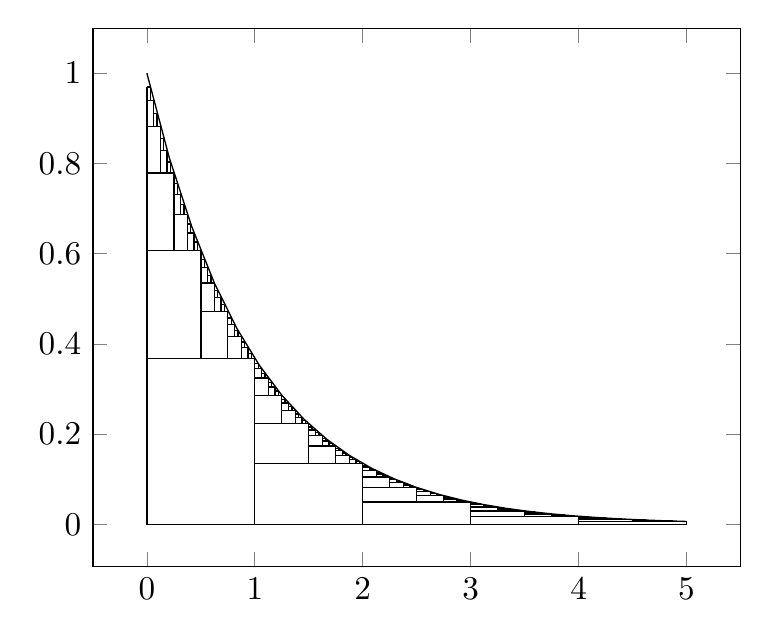
\begin{tikzpicture}[scale=1.2]
\begin{axis}
\addplot[domain=0:5] {e^(-x)};
\draw (axis cs: 0, 0) -- (axis cs: 5, 0);
\draw (axis cs: 0, 0) -- (axis cs: 0, 0.36787944160372466);
\draw (axis cs: 1, 0) -- (axis cs: 1, 0.36787944160372466);
\draw (axis cs: 0, 0.36787944160372466) -- (axis cs: 1, 0.36787944160372466);
\draw (axis cs: 0, 0.36787944160372466) -- (axis cs: 0, 0.6065306600659573);
\draw (axis cs: 1/2, 0.36787944160372466) -- (axis cs: 1/2, 0.6065306600659573);
\draw (axis cs: 0, 0.6065306600659573) -- (axis cs: 1/2, 0.6065306600659573);
\draw (axis cs: 1/2, 0.36787944160372466) -- (axis cs: 1/2, 0.36787944182176296);
\draw (axis cs: 1, 0.36787944160372466) -- (axis cs: 1, 0.36787944182176296);
\draw (axis cs: 1/2, 0.36787944182176296) -- (axis cs: 1, 0.36787944182176296);
\draw (axis cs: 0, 0.6065306600659573) -- (axis cs: 0, 0.7788007832943493);
\draw (axis cs: 1/4, 0.6065306600659573) -- (axis cs: 1/4, 0.7788007832943493);
\draw (axis cs: 0, 0.7788007832943493) -- (axis cs: 1/4, 0.7788007832943493);
\draw (axis cs: 1/4, 0.6065306600659573) -- (axis cs: 1/4, 0.6065306602487321);
\draw (axis cs: 1/2, 0.6065306600659573) -- (axis cs: 1/2, 0.6065306602487321);
\draw (axis cs: 1/4, 0.6065306602487321) -- (axis cs: 1/2, 0.6065306602487321);
\draw (axis cs: 1/2, 0.36787944182176296) -- (axis cs: 1/2, 0.4723665534165668);
\draw (axis cs: 3/4, 0.36787944182176296) -- (axis cs: 3/4, 0.4723665534165668);
\draw (axis cs: 1/2, 0.4723665534165668) -- (axis cs: 3/4, 0.4723665534165668);
\draw (axis cs: 3/4, 0.36787944182176296) -- (axis cs: 3/4, 0.36787944165116493);
\draw (axis cs: 1, 0.36787944182176296) -- (axis cs: 1, 0.36787944165116493);
\draw (axis cs: 3/4, 0.36787944165116493) -- (axis cs: 1, 0.36787944165116493);
\draw (axis cs: 0, 0.7788007832943493) -- (axis cs: 0, 0.8824969027064975);
\draw (axis cs: 1/8, 0.7788007832943493) -- (axis cs: 1/8, 0.8824969027064975);
\draw (axis cs: 0, 0.8824969027064975) -- (axis cs: 1/8, 0.8824969027064975);
\draw (axis cs: 1/8, 0.7788007832943493) -- (axis cs: 1/8, 0.7788007834155871);
\draw (axis cs: 1/4, 0.7788007832943493) -- (axis cs: 1/4, 0.7788007834155871);
\draw (axis cs: 1/8, 0.7788007834155871) -- (axis cs: 1/4, 0.7788007834155871);
\draw (axis cs: 1/4, 0.6065306602487321) -- (axis cs: 1/4, 0.6872892792824334);
\draw (axis cs: 3/8, 0.6065306602487321) -- (axis cs: 3/8, 0.6872892792824334);
\draw (axis cs: 1/4, 0.6872892792824334) -- (axis cs: 3/8, 0.6872892792824334);
\draw (axis cs: 3/8, 0.6065306602487321) -- (axis cs: 3/8, 0.6065306601050652);
\draw (axis cs: 1/2, 0.6065306602487321) -- (axis cs: 1/2, 0.6065306601050652);
\draw (axis cs: 3/8, 0.6065306601050652) -- (axis cs: 1/2, 0.6065306601050652);
\draw (axis cs: 1/2, 0.4723665534165668) -- (axis cs: 1/2, 0.5352614291382933);
\draw (axis cs: 5/8, 0.4723665534165668) -- (axis cs: 5/8, 0.5352614291382933);
\draw (axis cs: 1/2, 0.5352614291382933) -- (axis cs: 5/8, 0.5352614291382933);
\draw (axis cs: 5/8, 0.4723665534165668) -- (axis cs: 5/8, 0.47236655326632526);
\draw (axis cs: 3/4, 0.4723665534165668) -- (axis cs: 3/4, 0.47236655326632526);
\draw (axis cs: 5/8, 0.47236655326632526) -- (axis cs: 3/4, 0.47236655326632526);
\draw (axis cs: 3/4, 0.36787944165116493) -- (axis cs: 3/4, 0.4168620200899856);
\draw (axis cs: 7/8, 0.36787944165116493) -- (axis cs: 7/8, 0.4168620200899856);
\draw (axis cs: 3/4, 0.4168620200899856) -- (axis cs: 7/8, 0.4168620200899856);
\draw (axis cs: 7/8, 0.36787944165116493) -- (axis cs: 7/8, 0.36787944186014293);
\draw (axis cs: 1, 0.36787944165116493) -- (axis cs: 1, 0.36787944186014293);
\draw (axis cs: 7/8, 0.36787944186014293) -- (axis cs: 1, 0.36787944186014293);
\draw (axis cs: 0, 0.8824969027064975) -- (axis cs: 0, 0.9394130629417682);
\draw (axis cs: 1/16, 0.8824969027064975) -- (axis cs: 1/16, 0.9394130629417682);
\draw (axis cs: 0, 0.9394130629417682) -- (axis cs: 1/16, 0.9394130629417682);
\draw (axis cs: 1/16, 0.8824969027064975) -- (axis cs: 1/16, 0.8824969027796001);
\draw (axis cs: 1/8, 0.8824969027064975) -- (axis cs: 1/8, 0.8824969027796001);
\draw (axis cs: 1/16, 0.8824969027796001) -- (axis cs: 1/8, 0.8824969027796001);
\draw (axis cs: 1/8, 0.7788007834155871) -- (axis cs: 1/8, 0.829029118476808);
\draw (axis cs: 3/16, 0.7788007834155871) -- (axis cs: 3/16, 0.829029118476808);
\draw (axis cs: 1/8, 0.829029118476808) -- (axis cs: 3/16, 0.829029118476808);
\draw (axis cs: 3/16, 0.7788007834155871) -- (axis cs: 3/16, 0.778800783319457);
\draw (axis cs: 1/4, 0.7788007834155871) -- (axis cs: 1/4, 0.778800783319457);
\draw (axis cs: 3/16, 0.778800783319457) -- (axis cs: 1/4, 0.778800783319457);
\draw (axis cs: 1/4, 0.6872892792824334) -- (axis cs: 1/4, 0.7316156293698852);
\draw (axis cs: 5/16, 0.6872892792824334) -- (axis cs: 5/16, 0.7316156293698852);
\draw (axis cs: 1/4, 0.7316156293698852) -- (axis cs: 5/16, 0.7316156293698852);
\draw (axis cs: 5/16, 0.6872892792824334) -- (axis cs: 5/16, 0.687289279169697);
\draw (axis cs: 3/8, 0.6872892792824334) -- (axis cs: 3/8, 0.687289279169697);
\draw (axis cs: 5/16, 0.687289279169697) -- (axis cs: 3/8, 0.687289279169697);
\draw (axis cs: 3/8, 0.6065306601050652) -- (axis cs: 3/8, 0.645648526743318);
\draw (axis cs: 7/16, 0.6065306601050652) -- (axis cs: 7/16, 0.645648526743318);
\draw (axis cs: 3/8, 0.645648526743318) -- (axis cs: 7/16, 0.645648526743318);
\draw (axis cs: 7/16, 0.6065306601050652) -- (axis cs: 7/16, 0.6065306602803711);
\draw (axis cs: 1/2, 0.6065306601050652) -- (axis cs: 1/2, 0.6065306602803711);
\draw (axis cs: 7/16, 0.6065306602803711) -- (axis cs: 1/2, 0.6065306602803711);
\draw (axis cs: 1/2, 0.5352614291382933) -- (axis cs: 1/2, 0.5697828252642633);
\draw (axis cs: 9/16, 0.5352614291382933) -- (axis cs: 9/16, 0.5697828252642633);
\draw (axis cs: 1/2, 0.5697828252642633) -- (axis cs: 9/16, 0.5697828252642633);
\draw (axis cs: 9/16, 0.5352614291382933) -- (axis cs: 9/16, 0.5352614289897776);
\draw (axis cs: 5/8, 0.5352614291382933) -- (axis cs: 5/8, 0.5352614289897776);
\draw (axis cs: 9/16, 0.5352614289897776) -- (axis cs: 5/8, 0.5352614289897776);
\draw (axis cs: 5/8, 0.47236655326632526) -- (axis cs: 5/8, 0.5028315783817777);
\draw (axis cs: 11/16, 0.47236655326632526) -- (axis cs: 11/16, 0.5028315783817777);
\draw (axis cs: 5/8, 0.5028315783817777) -- (axis cs: 11/16, 0.5028315783817777);
\draw (axis cs: 11/16, 0.47236655326632526) -- (axis cs: 11/16, 0.4723665534564358);
\draw (axis cs: 3/4, 0.47236655326632526) -- (axis cs: 3/4, 0.4723665534564358);
\draw (axis cs: 11/16, 0.4723665534564358) -- (axis cs: 3/4, 0.4723665534564358);
\draw (axis cs: 3/4, 0.4168620200899856) -- (axis cs: 3/4, 0.4437473107531558);
\draw (axis cs: 13/16, 0.4168620200899856) -- (axis cs: 13/16, 0.4437473107531558);
\draw (axis cs: 3/4, 0.4437473107531558) -- (axis cs: 13/16, 0.4437473107531558);
\draw (axis cs: 13/16, 0.4168620200899856) -- (axis cs: 13/16, 0.4168620203098653);
\draw (axis cs: 7/8, 0.4168620200899856) -- (axis cs: 7/8, 0.4168620203098653);
\draw (axis cs: 13/16, 0.4168620203098653) -- (axis cs: 7/8, 0.4168620203098653);
\draw (axis cs: 7/8, 0.36787944186014293) -- (axis cs: 7/8, 0.3916056272654166);
\draw (axis cs: 15/16, 0.36787944186014293) -- (axis cs: 15/16, 0.3916056272654166);
\draw (axis cs: 7/8, 0.3916056272654166) -- (axis cs: 15/16, 0.3916056272654166);
\draw (axis cs: 15/16, 0.36787944186014293) -- (axis cs: 15/16, 0.3678794417014049);
\draw (axis cs: 1, 0.36787944186014293) -- (axis cs: 1, 0.3678794417014049);
\draw (axis cs: 15/16, 0.3678794417014049) -- (axis cs: 1, 0.3678794417014049);
\draw (axis cs: 0, 0.9394130629417682) -- (axis cs: 0, 0.9692332345425265);
\draw (axis cs: 1/32, 0.9394130629417682) -- (axis cs: 1/32, 0.9692332345425265);
\draw (axis cs: 0, 0.9692332345425265) -- (axis cs: 1/32, 0.9692332345425265);
\draw (axis cs: 1/32, 0.9394130629417682) -- (axis cs: 1/32, 0.9394130629133053);
\draw (axis cs: 1/16, 0.9394130629417682) -- (axis cs: 1/16, 0.9394130629133053);
\draw (axis cs: 1/32, 0.9394130629133053) -- (axis cs: 1/16, 0.9394130629133053);
\draw (axis cs: 1/16, 0.8824969027796001) -- (axis cs: 1/16, 0.9105103615428042);
\draw (axis cs: 3/32, 0.8824969027796001) -- (axis cs: 3/32, 0.9105103615428042);
\draw (axis cs: 1/16, 0.9105103615428042) -- (axis cs: 3/32, 0.9105103615428042);
\draw (axis cs: 3/32, 0.8824969027796001) -- (axis cs: 3/32, 0.8824969027207229);
\draw (axis cs: 1/8, 0.8824969027796001) -- (axis cs: 1/8, 0.8824969027207229);
\draw (axis cs: 3/32, 0.8824969027207229) -- (axis cs: 1/8, 0.8824969027207229);
\draw (axis cs: 1/8, 0.829029118476808) -- (axis cs: 1/8, 0.8553453275548334);
\draw (axis cs: 5/32, 0.829029118476808) -- (axis cs: 5/32, 0.8553453275548334);
\draw (axis cs: 1/8, 0.8553453275548334) -- (axis cs: 5/32, 0.8553453275548334);
\draw (axis cs: 5/32, 0.829029118476808) -- (axis cs: 5/32, 0.8290291184046698);
\draw (axis cs: 3/16, 0.829029118476808) -- (axis cs: 3/16, 0.8290291184046698);
\draw (axis cs: 5/32, 0.8290291184046698) -- (axis cs: 3/16, 0.8290291184046698);
\draw (axis cs: 3/16, 0.778800783319457) -- (axis cs: 3/16, 0.8035225738813201);
\draw (axis cs: 7/32, 0.778800783319457) -- (axis cs: 7/32, 0.8035225738813201);
\draw (axis cs: 3/16, 0.8035225738813201) -- (axis cs: 7/32, 0.8035225738813201);
\draw (axis cs: 7/32, 0.778800783319457) -- (axis cs: 7/32, 0.7788007834358996);
\draw (axis cs: 1/4, 0.778800783319457) -- (axis cs: 1/4, 0.7788007834358996);
\draw (axis cs: 7/32, 0.7788007834358996) -- (axis cs: 1/4, 0.7788007834358996);
\draw (axis cs: 1/4, 0.7316156293698852) -- (axis cs: 1/4, 0.7548396023407801);
\draw (axis cs: 9/32, 0.7316156293698852) -- (axis cs: 9/32, 0.7548396023407801);
\draw (axis cs: 1/4, 0.7548396023407801) -- (axis cs: 9/32, 0.7548396023407801);
\draw (axis cs: 9/32, 0.7316156293698852) -- (axis cs: 9/32, 0.7316156292647287);
\draw (axis cs: 5/16, 0.7316156293698852) -- (axis cs: 5/16, 0.7316156292647287);
\draw (axis cs: 9/32, 0.7316156292647287) -- (axis cs: 5/16, 0.7316156292647287);
\draw (axis cs: 5/16, 0.687289279169697) -- (axis cs: 5/16, 0.7091061827235392);
\draw (axis cs: 11/32, 0.687289279169697) -- (axis cs: 11/32, 0.7091061827235392);
\draw (axis cs: 5/16, 0.7091061827235392) -- (axis cs: 11/32, 0.7091061827235392);
\draw (axis cs: 11/32, 0.687289279169697) -- (axis cs: 11/32, 0.687289279311438);
\draw (axis cs: 3/8, 0.687289279169697) -- (axis cs: 3/8, 0.687289279311438);
\draw (axis cs: 11/32, 0.687289279311438) -- (axis cs: 3/8, 0.687289279311438);
\draw (axis cs: 3/8, 0.645648526743318) -- (axis cs: 3/8, 0.6661436112079405);
\draw (axis cs: 13/32, 0.645648526743318) -- (axis cs: 13/32, 0.6661436112079405);
\draw (axis cs: 3/8, 0.6661436112079405) -- (axis cs: 13/32, 0.6661436112079405);
\draw (axis cs: 13/32, 0.645648526743318) -- (axis cs: 13/32, 0.6456485269168244);
\draw (axis cs: 7/16, 0.645648526743318) -- (axis cs: 7/16, 0.6456485269168244);
\draw (axis cs: 13/32, 0.6456485269168244) -- (axis cs: 7/16, 0.6456485269168244);
\draw (axis cs: 7/16, 0.6065306602803711) -- (axis cs: 7/16, 0.6257840100717663);
\draw (axis cs: 15/32, 0.6065306602803711) -- (axis cs: 15/32, 0.6257840100717663);
\draw (axis cs: 7/16, 0.6257840100717663) -- (axis cs: 15/32, 0.6257840100717663);
\draw (axis cs: 15/32, 0.6065306602803711) -- (axis cs: 15/32, 0.606530660146481);
\draw (axis cs: 1/2, 0.6065306602803711) -- (axis cs: 1/2, 0.606530660146481);
\draw (axis cs: 15/32, 0.606530660146481) -- (axis cs: 1/2, 0.606530660146481);
\draw (axis cs: 1/2, 0.5697828252642633) -- (axis cs: 1/2, 0.5878696735244751);
\draw (axis cs: 17/32, 0.5697828252642633) -- (axis cs: 17/32, 0.5878696735244751);
\draw (axis cs: 1/2, 0.5878696735244751) -- (axis cs: 17/32, 0.5878696735244751);
\draw (axis cs: 17/32, 0.5697828252642633) -- (axis cs: 17/32, 0.5697828251028737);
\draw (axis cs: 9/16, 0.5697828252642633) -- (axis cs: 9/16, 0.5697828251028737);
\draw (axis cs: 17/32, 0.5697828251028737) -- (axis cs: 9/16, 0.5697828251028737);
\draw (axis cs: 9/16, 0.5352614289897776) -- (axis cs: 9/16, 0.5522524505062694);
\draw (axis cs: 19/32, 0.5352614289897776) -- (axis cs: 19/32, 0.5522524505062694);
\draw (axis cs: 9/16, 0.5522524505062694) -- (axis cs: 19/32, 0.5522524505062694);
\draw (axis cs: 19/32, 0.5352614289897776) -- (axis cs: 19/32, 0.5352614291748428);
\draw (axis cs: 5/8, 0.5352614289897776) -- (axis cs: 5/8, 0.5352614291748428);
\draw (axis cs: 19/32, 0.5352614291748428) -- (axis cs: 5/8, 0.5352614291748428);
\draw (axis cs: 5/8, 0.5028315783817777) -- (axis cs: 5/8, 0.5187931662895634);
\draw (axis cs: 21/32, 0.5028315783817777) -- (axis cs: 21/32, 0.5187931662895634);
\draw (axis cs: 5/8, 0.5187931662895634) -- (axis cs: 21/32, 0.5187931662895634);
\draw (axis cs: 21/32, 0.5028315783817777) -- (axis cs: 21/32, 0.5028315785870574);
\draw (axis cs: 11/16, 0.5028315783817777) -- (axis cs: 11/16, 0.5028315785870574);
\draw (axis cs: 21/32, 0.5028315785870574) -- (axis cs: 11/16, 0.5028315785870574);
\draw (axis cs: 11/16, 0.4723665534564358) -- (axis cs: 11/16, 0.4873610773107796);
\draw (axis cs: 23/32, 0.4723665534564358) -- (axis cs: 23/32, 0.4873610773107796);
\draw (axis cs: 11/16, 0.4873610773107796) -- (axis cs: 23/32, 0.4873610773107796);
\draw (axis cs: 23/32, 0.4723665534564358) -- (axis cs: 23/32, 0.4723665533185145);
\draw (axis cs: 3/4, 0.4723665534564358) -- (axis cs: 3/4, 0.4723665533185145);
\draw (axis cs: 23/32, 0.4723665533185145) -- (axis cs: 3/4, 0.4723665533185145);
\draw (axis cs: 3/4, 0.4437473107531558) -- (axis cs: 3/4, 0.45783336231703897);
\draw (axis cs: 25/32, 0.4437473107531558) -- (axis cs: 25/32, 0.45783336231703897);
\draw (axis cs: 3/4, 0.45783336231703897) -- (axis cs: 25/32, 0.45783336231703897);
\draw (axis cs: 25/32, 0.4437473107531558) -- (axis cs: 25/32, 0.4437473105958565);
\draw (axis cs: 13/16, 0.4437473107531558) -- (axis cs: 13/16, 0.4437473105958565);
\draw (axis cs: 25/32, 0.4437473105958565) -- (axis cs: 13/16, 0.4437473105958565);
\draw (axis cs: 13/16, 0.4168620203098653) -- (axis cs: 13/16, 0.4300946411255604);
\draw (axis cs: 27/32, 0.4168620203098653) -- (axis cs: 27/32, 0.4300946411255604);
\draw (axis cs: 13/16, 0.4300946411255604) -- (axis cs: 27/32, 0.4300946411255604);
\draw (axis cs: 27/32, 0.4168620203098653) -- (axis cs: 27/32, 0.4168620201360424);
\draw (axis cs: 7/8, 0.4168620203098653) -- (axis cs: 7/8, 0.4168620201360424);
\draw (axis cs: 27/32, 0.4168620201360424) -- (axis cs: 7/8, 0.4168620201360424);
\draw (axis cs: 7/8, 0.3916056272654166) -- (axis cs: 7/8, 0.4040365240941731);
\draw (axis cs: 29/32, 0.3916056272654166) -- (axis cs: 29/32, 0.4040365240941731);
\draw (axis cs: 7/8, 0.4040365240941731) -- (axis cs: 29/32, 0.4040365240941731);
\draw (axis cs: 29/32, 0.3916056272654166) -- (axis cs: 29/32, 0.3916056270821371);
\draw (axis cs: 15/16, 0.3916056272654166) -- (axis cs: 15/16, 0.3916056270821371);
\draw (axis cs: 29/32, 0.3916056270821371) -- (axis cs: 15/16, 0.3916056270821371);
\draw (axis cs: 15/16, 0.3678794417014049) -- (axis cs: 15/16, 0.37955718856409554);
\draw (axis cs: 31/32, 0.3678794417014049) -- (axis cs: 31/32, 0.37955718856409554);
\draw (axis cs: 15/16, 0.37955718856409554) -- (axis cs: 31/32, 0.37955718856409554);
\draw (axis cs: 31/32, 0.3678794417014049) -- (axis cs: 31/32, 0.367879441900788);
\draw (axis cs: 1, 0.3678794417014049) -- (axis cs: 1, 0.367879441900788);
\draw (axis cs: 31/32, 0.367879441900788) -- (axis cs: 1, 0.367879441900788);
\draw (axis cs: 1, 0) -- (axis cs: 1, 0.1353352833956405);
\draw (axis cs: 2, 0) -- (axis cs: 2, 0.1353352833956405);
\draw (axis cs: 1, 0.1353352833956405) -- (axis cs: 2, 0.1353352833956405);
\draw (axis cs: 1, 0.1353352833956405) -- (axis cs: 1, 0.22313016027841043);
\draw (axis cs: 3/2, 0.1353352833956405) -- (axis cs: 3/2, 0.22313016027841043);
\draw (axis cs: 1, 0.22313016027841043) -- (axis cs: 3/2, 0.22313016027841043);
\draw (axis cs: 3/2, 0.1353352833956405) -- (axis cs: 3/2, 0.1353352834758523);
\draw (axis cs: 2, 0.1353352833956405) -- (axis cs: 2, 0.1353352834758523);
\draw (axis cs: 3/2, 0.1353352834758523) -- (axis cs: 2, 0.1353352834758523);
\draw (axis cs: 1, 0.22313016027841043) -- (axis cs: 1, 0.28650479694220676);
\draw (axis cs: 5/4, 0.22313016027841043) -- (axis cs: 5/4, 0.28650479694220676);
\draw (axis cs: 1, 0.28650479694220676) -- (axis cs: 5/4, 0.28650479694220676);
\draw (axis cs: 5/4, 0.22313016027841043) -- (axis cs: 5/4, 0.22313016034564953);
\draw (axis cs: 3/2, 0.22313016027841043) -- (axis cs: 3/2, 0.22313016034564953);
\draw (axis cs: 5/4, 0.22313016034564953) -- (axis cs: 3/2, 0.22313016034564953);
\draw (axis cs: 3/2, 0.1353352834758523) -- (axis cs: 3/2, 0.17377394369896684);
\draw (axis cs: 7/4, 0.1353352834758523) -- (axis cs: 7/4, 0.17377394369896684);
\draw (axis cs: 3/2, 0.17377394369896684) -- (axis cs: 7/4, 0.17377394369896684);
\draw (axis cs: 7/4, 0.1353352834758523) -- (axis cs: 7/4, 0.13533528341309278);
\draw (axis cs: 2, 0.1353352834758523) -- (axis cs: 2, 0.13533528341309278);
\draw (axis cs: 7/4, 0.13533528341309278) -- (axis cs: 2, 0.13533528341309278);
\draw (axis cs: 1, 0.28650479694220676) -- (axis cs: 1, 0.324652467403195);
\draw (axis cs: 9/8, 0.28650479694220676) -- (axis cs: 9/8, 0.324652467403195);
\draw (axis cs: 1, 0.324652467403195) -- (axis cs: 9/8, 0.324652467403195);
\draw (axis cs: 9/8, 0.28650479694220676) -- (axis cs: 9/8, 0.28650479698680764);
\draw (axis cs: 5/4, 0.28650479694220676) -- (axis cs: 5/4, 0.28650479698680764);
\draw (axis cs: 9/8, 0.28650479698680764) -- (axis cs: 5/4, 0.28650479698680764);
\draw (axis cs: 5/4, 0.22313016034564953) -- (axis cs: 5/4, 0.252839595985545);
\draw (axis cs: 11/8, 0.22313016034564953) -- (axis cs: 11/8, 0.252839595985545);
\draw (axis cs: 5/4, 0.252839595985545) -- (axis cs: 11/8, 0.252839595985545);
\draw (axis cs: 11/8, 0.22313016034564953) -- (axis cs: 11/8, 0.22313016029279742);
\draw (axis cs: 3/2, 0.22313016034564953) -- (axis cs: 3/2, 0.22313016029279742);
\draw (axis cs: 11/8, 0.22313016029279742) -- (axis cs: 3/2, 0.22313016029279742);
\draw (axis cs: 3/2, 0.17377394369896684) -- (axis cs: 3/2, 0.19691167543202293);
\draw (axis cs: 13/8, 0.17377394369896684) -- (axis cs: 13/8, 0.19691167543202293);
\draw (axis cs: 3/2, 0.19691167543202293) -- (axis cs: 13/8, 0.19691167543202293);
\draw (axis cs: 13/8, 0.17377394369896684) -- (axis cs: 13/8, 0.17377394364369608);
\draw (axis cs: 7/4, 0.17377394369896684) -- (axis cs: 7/4, 0.17377394364369608);
\draw (axis cs: 13/8, 0.17377394364369608) -- (axis cs: 7/4, 0.17377394364369608);
\draw (axis cs: 7/4, 0.13533528341309278) -- (axis cs: 7/4, 0.15335496699630247);
\draw (axis cs: 15/8, 0.13533528341309278) -- (axis cs: 15/8, 0.15335496699630247);
\draw (axis cs: 7/4, 0.15335496699630247) -- (axis cs: 15/8, 0.15335496699630247);
\draw (axis cs: 15/8, 0.13533528341309278) -- (axis cs: 15/8, 0.1353352834899715);
\draw (axis cs: 2, 0.13533528341309278) -- (axis cs: 2, 0.1353352834899715);
\draw (axis cs: 15/8, 0.1353352834899715) -- (axis cs: 2, 0.1353352834899715);
\draw (axis cs: 1, 0.324652467403195) -- (axis cs: 1, 0.34559075262417066);
\draw (axis cs: 17/16, 0.324652467403195) -- (axis cs: 17/16, 0.34559075262417066);
\draw (axis cs: 1, 0.34559075262417066) -- (axis cs: 17/16, 0.34559075262417066);
\draw (axis cs: 17/16, 0.324652467403195) -- (axis cs: 17/16, 0.324652467430088);
\draw (axis cs: 9/8, 0.324652467403195) -- (axis cs: 9/8, 0.324652467430088);
\draw (axis cs: 17/16, 0.324652467430088) -- (axis cs: 9/8, 0.324652467430088);
\draw (axis cs: 9/8, 0.28650479698680764) -- (axis cs: 9/8, 0.3049827688201016);
\draw (axis cs: 19/16, 0.28650479698680764) -- (axis cs: 19/16, 0.3049827688201016);
\draw (axis cs: 9/8, 0.3049827688201016) -- (axis cs: 19/16, 0.3049827688201016);
\draw (axis cs: 19/16, 0.28650479698680764) -- (axis cs: 19/16, 0.2865047969514434);
\draw (axis cs: 5/4, 0.28650479698680764) -- (axis cs: 5/4, 0.2865047969514434);
\draw (axis cs: 19/16, 0.2865047969514434) -- (axis cs: 5/4, 0.2865047969514434);
\draw (axis cs: 5/4, 0.252839595985545) -- (axis cs: 5/4, 0.2691463488848865);
\draw (axis cs: 21/16, 0.252839595985545) -- (axis cs: 21/16, 0.2691463488848865);
\draw (axis cs: 5/4, 0.2691463488848865) -- (axis cs: 21/16, 0.2691463488848865);
\draw (axis cs: 21/16, 0.252839595985545) -- (axis cs: 21/16, 0.2528395959440715);
\draw (axis cs: 11/8, 0.252839595985545) -- (axis cs: 11/8, 0.2528395959440715);
\draw (axis cs: 21/16, 0.2528395959440715) -- (axis cs: 11/8, 0.2528395959440715);
\draw (axis cs: 11/8, 0.22313016029279742) -- (axis cs: 11/8, 0.23752081921149684);
\draw (axis cs: 23/16, 0.22313016029279742) -- (axis cs: 23/16, 0.23752081921149684);
\draw (axis cs: 11/8, 0.23752081921149684) -- (axis cs: 23/16, 0.23752081921149684);
\draw (axis cs: 23/16, 0.22313016029279742) -- (axis cs: 23/16, 0.22313016035728886);
\draw (axis cs: 3/2, 0.22313016029279742) -- (axis cs: 3/2, 0.22313016035728886);
\draw (axis cs: 23/16, 0.22313016035728886) -- (axis cs: 3/2, 0.22313016035728886);
\draw (axis cs: 3/2, 0.19691167543202293) -- (axis cs: 3/2, 0.20961138734730272);
\draw (axis cs: 25/16, 0.19691167543202293) -- (axis cs: 25/16, 0.20961138734730272);
\draw (axis cs: 3/2, 0.20961138734730272) -- (axis cs: 25/16, 0.20961138734730272);
\draw (axis cs: 25/16, 0.19691167543202293) -- (axis cs: 25/16, 0.19691167537738702);
\draw (axis cs: 13/8, 0.19691167543202293) -- (axis cs: 13/8, 0.19691167537738702);
\draw (axis cs: 25/16, 0.19691167537738702) -- (axis cs: 13/8, 0.19691167537738702);
\draw (axis cs: 13/8, 0.17377394364369608) -- (axis cs: 13/8, 0.18498140005844269);
\draw (axis cs: 27/16, 0.17377394364369608) -- (axis cs: 27/16, 0.18498140005844269);
\draw (axis cs: 13/8, 0.18498140005844269) -- (axis cs: 27/16, 0.18498140005844269);
\draw (axis cs: 27/16, 0.17377394364369608) -- (axis cs: 27/16, 0.17377394371363383);
\draw (axis cs: 7/4, 0.17377394364369608) -- (axis cs: 7/4, 0.17377394371363383);
\draw (axis cs: 27/16, 0.17377394371363383) -- (axis cs: 7/4, 0.17377394371363383);
\draw (axis cs: 7/4, 0.15335496699630247) -- (axis cs: 7/4, 0.16324551270120133);
\draw (axis cs: 29/16, 0.15335496699630247) -- (axis cs: 29/16, 0.16324551270120133);
\draw (axis cs: 7/4, 0.16324551270120133) -- (axis cs: 29/16, 0.16324551270120133);
\draw (axis cs: 29/16, 0.15335496699630247) -- (axis cs: 29/16, 0.15335496707719168);
\draw (axis cs: 15/8, 0.15335496699630247) -- (axis cs: 15/8, 0.15335496707719168);
\draw (axis cs: 29/16, 0.15335496707719168) -- (axis cs: 15/8, 0.15335496707719168);
\draw (axis cs: 15/8, 0.1353352834899715) -- (axis cs: 15/8, 0.1440636593179936);
\draw (axis cs: 31/16, 0.1353352834899715) -- (axis cs: 31/16, 0.1440636593179936);
\draw (axis cs: 15/8, 0.1440636593179936) -- (axis cs: 31/16, 0.1440636593179936);
\draw (axis cs: 31/16, 0.1353352834899715) -- (axis cs: 31/16, 0.13533528343157503);
\draw (axis cs: 2, 0.1353352834899715) -- (axis cs: 2, 0.13533528343157503);
\draw (axis cs: 31/16, 0.13533528343157503) -- (axis cs: 2, 0.13533528343157503);
\draw (axis cs: 1, 0.34559075262417066) -- (axis cs: 1, 0.35656098068829417);
\draw (axis cs: 33/32, 0.34559075262417066) -- (axis cs: 33/32, 0.35656098068829417);
\draw (axis cs: 1, 0.35656098068829417) -- (axis cs: 33/32, 0.35656098068829417);
\draw (axis cs: 33/32, 0.34559075262417066) -- (axis cs: 33/32, 0.3455907526136997);
\draw (axis cs: 17/16, 0.34559075262417066) -- (axis cs: 17/16, 0.3455907526136997);
\draw (axis cs: 33/32, 0.3455907526136997) -- (axis cs: 17/16, 0.3455907526136997);
\draw (axis cs: 17/16, 0.324652467430088) -- (axis cs: 17/16, 0.3349580429851747);
\draw (axis cs: 35/32, 0.324652467430088) -- (axis cs: 35/32, 0.3349580429851747);
\draw (axis cs: 17/16, 0.3349580429851747) -- (axis cs: 35/32, 0.3349580429851747);
\draw (axis cs: 35/32, 0.324652467430088) -- (axis cs: 35/32, 0.32465246740842824);
\draw (axis cs: 9/8, 0.324652467430088) -- (axis cs: 9/8, 0.32465246740842824);
\draw (axis cs: 35/32, 0.32465246740842824) -- (axis cs: 9/8, 0.32465246740842824);
\draw (axis cs: 9/8, 0.3049827688201016) -- (axis cs: 9/8, 0.3146639611094764);
\draw (axis cs: 37/32, 0.3049827688201016) -- (axis cs: 37/32, 0.3146639611094764);
\draw (axis cs: 9/8, 0.3146639611094764) -- (axis cs: 37/32, 0.3146639611094764);
\draw (axis cs: 37/32, 0.3049827688201016) -- (axis cs: 37/32, 0.3049827687935634);
\draw (axis cs: 19/16, 0.3049827688201016) -- (axis cs: 19/16, 0.3049827687935634);
\draw (axis cs: 37/32, 0.3049827687935634) -- (axis cs: 19/16, 0.3049827687935634);
\draw (axis cs: 19/16, 0.2865047969514434) -- (axis cs: 19/16, 0.295599435448099);
\draw (axis cs: 39/32, 0.2865047969514434) -- (axis cs: 39/32, 0.295599435448099);
\draw (axis cs: 19/16, 0.295599435448099) -- (axis cs: 39/32, 0.295599435448099);
\draw (axis cs: 39/32, 0.2865047969514434) -- (axis cs: 39/32, 0.2865047969942802);
\draw (axis cs: 5/4, 0.2865047969514434) -- (axis cs: 5/4, 0.2865047969942802);
\draw (axis cs: 39/32, 0.2865047969942802) -- (axis cs: 5/4, 0.2865047969942802);
\draw (axis cs: 5/4, 0.2691463488848865) -- (axis cs: 5/4, 0.2776899710831999);
\draw (axis cs: 41/32, 0.2691463488848865) -- (axis cs: 41/32, 0.2776899710831999);
\draw (axis cs: 5/4, 0.2776899710831999) -- (axis cs: 41/32, 0.2776899710831999);
\draw (axis cs: 41/32, 0.2691463488848865) -- (axis cs: 41/32, 0.2691463488462015);
\draw (axis cs: 21/16, 0.2691463488848865) -- (axis cs: 21/16, 0.2691463488462015);
\draw (axis cs: 41/32, 0.2691463488462015) -- (axis cs: 21/16, 0.2691463488462015);
\draw (axis cs: 21/16, 0.2528395959440715) -- (axis cs: 21/16, 0.26086558623155026);
\draw (axis cs: 43/32, 0.2528395959440715) -- (axis cs: 43/32, 0.26086558623155026);
\draw (axis cs: 21/16, 0.26086558623155026) -- (axis cs: 43/32, 0.26086558623155026);
\draw (axis cs: 43/32, 0.2528395959440715) -- (axis cs: 43/32, 0.2528395959962152);
\draw (axis cs: 11/8, 0.2528395959440715) -- (axis cs: 11/8, 0.2528395959962152);
\draw (axis cs: 43/32, 0.2528395959962152) -- (axis cs: 11/8, 0.2528395959962152);
\draw (axis cs: 11/8, 0.23752081921149684) -- (axis cs: 11/8, 0.24506053943110373);
\draw (axis cs: 45/32, 0.23752081921149684) -- (axis cs: 45/32, 0.24506053943110373);
\draw (axis cs: 11/8, 0.24506053943110373) -- (axis cs: 45/32, 0.24506053943110373);
\draw (axis cs: 45/32, 0.23752081921149684) -- (axis cs: 45/32, 0.2375208192753263);
\draw (axis cs: 23/16, 0.23752081921149684) -- (axis cs: 23/16, 0.2375208192753263);
\draw (axis cs: 45/32, 0.2375208192753263) -- (axis cs: 23/16, 0.2375208192753263);
\draw (axis cs: 23/16, 0.22313016035728886) -- (axis cs: 23/16, 0.2302130719192256);
\draw (axis cs: 47/32, 0.22313016035728886) -- (axis cs: 47/32, 0.2302130719192256);
\draw (axis cs: 23/16, 0.2302130719192256) -- (axis cs: 47/32, 0.2302130719192256);
\draw (axis cs: 47/32, 0.22313016035728886) -- (axis cs: 47/32, 0.22313016030803345);
\draw (axis cs: 3/2, 0.22313016035728886) -- (axis cs: 3/2, 0.22313016030803345);
\draw (axis cs: 47/32, 0.22313016030803345) -- (axis cs: 3/2, 0.22313016030803345);
\draw (axis cs: 3/2, 0.20961138734730272) -- (axis cs: 3/2, 0.2162651669778221);
\draw (axis cs: 49/32, 0.20961138734730272) -- (axis cs: 49/32, 0.2162651669778221);
\draw (axis cs: 3/2, 0.2162651669778221) -- (axis cs: 49/32, 0.2162651669778221);
\draw (axis cs: 49/32, 0.20961138734730272) -- (axis cs: 49/32, 0.20961138728793083);
\draw (axis cs: 25/16, 0.20961138734730272) -- (axis cs: 25/16, 0.20961138728793083);
\draw (axis cs: 49/32, 0.20961138728793083) -- (axis cs: 25/16, 0.20961138728793083);
\draw (axis cs: 25/16, 0.19691167537738702) -- (axis cs: 25/16, 0.203162322877806);
\draw (axis cs: 51/32, 0.19691167537738702) -- (axis cs: 51/32, 0.203162322877806);
\draw (axis cs: 25/16, 0.203162322877806) -- (axis cs: 51/32, 0.203162322877806);
\draw (axis cs: 51/32, 0.19691167537738702) -- (axis cs: 51/32, 0.19691167544546867);
\draw (axis cs: 13/8, 0.19691167537738702) -- (axis cs: 13/8, 0.19691167544546867);
\draw (axis cs: 51/32, 0.19691167544546867) -- (axis cs: 13/8, 0.19691167544546867);
\draw (axis cs: 13/8, 0.18498140005844269) -- (axis cs: 13/8, 0.1908533400981677);
\draw (axis cs: 53/32, 0.18498140005844269) -- (axis cs: 53/32, 0.1908533400981677);
\draw (axis cs: 13/8, 0.1908533400981677) -- (axis cs: 53/32, 0.1908533400981677);
\draw (axis cs: 53/32, 0.18498140005844269) -- (axis cs: 53/32, 0.18498140013396083);
\draw (axis cs: 27/16, 0.18498140005844269) -- (axis cs: 27/16, 0.18498140013396083);
\draw (axis cs: 53/32, 0.18498140013396083) -- (axis cs: 27/16, 0.18498140013396083);
\draw (axis cs: 27/16, 0.17377394371363383) -- (axis cs: 27/16, 0.17929012076980166);
\draw (axis cs: 55/32, 0.17377394371363383) -- (axis cs: 55/32, 0.17929012076980166);
\draw (axis cs: 27/16, 0.17929012076980166) -- (axis cs: 55/32, 0.17929012076980166);
\draw (axis cs: 55/32, 0.17377394371363383) -- (axis cs: 55/32, 0.1737739436628954);
\draw (axis cs: 7/4, 0.17377394371363383) -- (axis cs: 7/4, 0.1737739436628954);
\draw (axis cs: 55/32, 0.1737739436628954) -- (axis cs: 7/4, 0.1737739436628954);
\draw (axis cs: 7/4, 0.16324551270120133) -- (axis cs: 7/4, 0.16842748147883477);
\draw (axis cs: 57/32, 0.16324551270120133) -- (axis cs: 57/32, 0.16842748147883477);
\draw (axis cs: 7/4, 0.16842748147883477) -- (axis cs: 57/32, 0.16842748147883477);
\draw (axis cs: 57/32, 0.16324551270120133) -- (axis cs: 57/32, 0.16324551264333415);
\draw (axis cs: 29/16, 0.16324551270120133) -- (axis cs: 29/16, 0.16324551264333415);
\draw (axis cs: 57/32, 0.16324551264333415) -- (axis cs: 29/16, 0.16324551264333415);
\draw (axis cs: 29/16, 0.15335496707719168) -- (axis cs: 29/16, 0.1582229762281032);
\draw (axis cs: 59/32, 0.15335496707719168) -- (axis cs: 59/32, 0.1582229762281032);
\draw (axis cs: 29/16, 0.1582229762281032) -- (axis cs: 59/32, 0.1582229762281032);
\draw (axis cs: 59/32, 0.15335496707719168) -- (axis cs: 59/32, 0.1533549670132458);
\draw (axis cs: 15/8, 0.15335496707719168) -- (axis cs: 15/8, 0.1533549670132458);
\draw (axis cs: 59/32, 0.1533549670132458) -- (axis cs: 15/8, 0.1533549670132458);
\draw (axis cs: 15/8, 0.1440636593179936) -- (axis cs: 15/8, 0.1486367306966164);
\draw (axis cs: 61/32, 0.1440636593179936) -- (axis cs: 61/32, 0.1486367306966164);
\draw (axis cs: 15/8, 0.1486367306966164) -- (axis cs: 61/32, 0.1486367306966164);
\draw (axis cs: 61/32, 0.1440636593179936) -- (axis cs: 61/32, 0.14406365925056883);
\draw (axis cs: 31/16, 0.1440636593179936) -- (axis cs: 31/16, 0.14406365925056883);
\draw (axis cs: 61/32, 0.14406365925056883) -- (axis cs: 31/16, 0.14406365925056883);
\draw (axis cs: 31/16, 0.13533528343157503) -- (axis cs: 31/16, 0.13963128642156322);
\draw (axis cs: 63/32, 0.13533528343157503) -- (axis cs: 63/32, 0.13963128642156322);
\draw (axis cs: 31/16, 0.13963128642156322) -- (axis cs: 63/32, 0.13963128642156322);
\draw (axis cs: 63/32, 0.13533528343157503) -- (axis cs: 63/32, 0.13533528350492396);
\draw (axis cs: 2, 0.13533528343157503) -- (axis cs: 2, 0.13533528350492396);
\draw (axis cs: 63/32, 0.13533528350492396) -- (axis cs: 2, 0.13533528350492396);
\draw (axis cs: 2, 0) -- (axis cs: 2, 0.049787068426367);
\draw (axis cs: 3, 0) -- (axis cs: 3, 0.049787068426367);
\draw (axis cs: 2, 0.049787068426367) -- (axis cs: 3, 0.049787068426367);
\draw (axis cs: 2, 0.049787068426367) -- (axis cs: 2, 0.082084998671716);
\draw (axis cs: 5/2, 0.049787068426367) -- (axis cs: 5/2, 0.082084998671716);
\draw (axis cs: 2, 0.082084998671716) -- (axis cs: 5/2, 0.082084998671716);
\draw (axis cs: 5/2, 0.049787068426367) -- (axis cs: 5/2, 0.04978706845587527);
\draw (axis cs: 3, 0.049787068426367) -- (axis cs: 3, 0.04978706845587527);
\draw (axis cs: 5/2, 0.04978706845587527) -- (axis cs: 3, 0.04978706845587527);
\draw (axis cs: 2, 0.082084998671716) -- (axis cs: 2, 0.10539922459203656);
\draw (axis cs: 9/4, 0.082084998671716) -- (axis cs: 9/4, 0.10539922459203656);
\draw (axis cs: 2, 0.10539922459203656) -- (axis cs: 9/4, 0.10539922459203656);
\draw (axis cs: 9/4, 0.082084998671716) -- (axis cs: 9/4, 0.08208499869645187);
\draw (axis cs: 5/2, 0.082084998671716) -- (axis cs: 5/2, 0.08208499869645187);
\draw (axis cs: 9/4, 0.08208499869645187) -- (axis cs: 5/2, 0.08208499869645187);
\draw (axis cs: 5/2, 0.04978706845587527) -- (axis cs: 5/2, 0.06392786129813362);
\draw (axis cs: 11/4, 0.04978706845587527) -- (axis cs: 11/4, 0.06392786129813362);
\draw (axis cs: 5/2, 0.06392786129813362) -- (axis cs: 11/4, 0.06392786129813362);
\draw (axis cs: 11/4, 0.04978706845587527) -- (axis cs: 11/4, 0.049787068432787344);
\draw (axis cs: 3, 0.04978706845587527) -- (axis cs: 3, 0.049787068432787344);
\draw (axis cs: 11/4, 0.049787068432787344) -- (axis cs: 3, 0.049787068432787344);
\draw (axis cs: 2, 0.10539922459203656) -- (axis cs: 2, 0.11943296828321726);
\draw (axis cs: 17/8, 0.10539922459203656) -- (axis cs: 17/8, 0.11943296828321726);
\draw (axis cs: 2, 0.11943296828321726) -- (axis cs: 17/8, 0.11943296828321726);
\draw (axis cs: 17/8, 0.10539922459203656) -- (axis cs: 17/8, 0.10539922460844436);
\draw (axis cs: 9/4, 0.10539922459203656) -- (axis cs: 9/4, 0.10539922460844436);
\draw (axis cs: 17/8, 0.10539922460844436) -- (axis cs: 9/4, 0.10539922460844436);
\draw (axis cs: 9/4, 0.08208499869645187) -- (axis cs: 9/4, 0.09301448927717554);
\draw (axis cs: 19/8, 0.08208499869645187) -- (axis cs: 19/8, 0.09301448927717554);
\draw (axis cs: 9/4, 0.09301448927717554) -- (axis cs: 19/8, 0.09301448927717554);
\draw (axis cs: 19/8, 0.08208499869645187) -- (axis cs: 19/8, 0.08208499867700865);
\draw (axis cs: 5/2, 0.08208499869645187) -- (axis cs: 5/2, 0.08208499867700865);
\draw (axis cs: 19/8, 0.08208499867700865) -- (axis cs: 5/2, 0.08208499867700865);
\draw (axis cs: 5/2, 0.06392786129813362) -- (axis cs: 5/2, 0.07243975711806502);
\draw (axis cs: 21/8, 0.06392786129813362) -- (axis cs: 21/8, 0.07243975711806502);
\draw (axis cs: 5/2, 0.07243975711806502) -- (axis cs: 21/8, 0.07243975711806502);
\draw (axis cs: 21/8, 0.06392786129813362) -- (axis cs: 21/8, 0.06392786127780062);
\draw (axis cs: 11/4, 0.06392786129813362) -- (axis cs: 11/4, 0.06392786127780062);
\draw (axis cs: 21/8, 0.06392786127780062) -- (axis cs: 11/4, 0.06392786127780062);
\draw (axis cs: 11/4, 0.049787068432787344) -- (axis cs: 11/4, 0.05641613955946473);
\draw (axis cs: 23/8, 0.049787068432787344) -- (axis cs: 23/8, 0.05641613955946473);
\draw (axis cs: 11/4, 0.05641613955946473) -- (axis cs: 23/8, 0.05641613955946473);
\draw (axis cs: 23/8, 0.049787068432787344) -- (axis cs: 23/8, 0.04978706846106944);
\draw (axis cs: 3, 0.049787068432787344) -- (axis cs: 3, 0.04978706846106944);
\draw (axis cs: 23/8, 0.04978706846106944) -- (axis cs: 3, 0.04978706846106944);
\draw (axis cs: 2, 0.11943296828321726) -- (axis cs: 2, 0.1271357329493981);
\draw (axis cs: 33/16, 0.11943296828321726) -- (axis cs: 33/16, 0.1271357329493981);
\draw (axis cs: 2, 0.1271357329493981) -- (axis cs: 33/16, 0.1271357329493981);
\draw (axis cs: 33/16, 0.11943296828321726) -- (axis cs: 33/16, 0.11943296829311066);
\draw (axis cs: 17/8, 0.11943296828321726) -- (axis cs: 17/8, 0.11943296829311066);
\draw (axis cs: 33/16, 0.11943296829311066) -- (axis cs: 17/8, 0.11943296829311066);
\draw (axis cs: 17/8, 0.10539922460844436) -- (axis cs: 17/8, 0.11219689056045815);
\draw (axis cs: 35/16, 0.10539922460844436) -- (axis cs: 35/16, 0.11219689056045815);
\draw (axis cs: 17/8, 0.11219689056045815) -- (axis cs: 35/16, 0.11219689056045815);
\draw (axis cs: 35/16, 0.10539922460844436) -- (axis cs: 35/16, 0.10539922459543453);
\draw (axis cs: 9/4, 0.10539922460844436) -- (axis cs: 9/4, 0.10539922459543453);
\draw (axis cs: 35/16, 0.10539922459543453) -- (axis cs: 9/4, 0.10539922459543453);
\draw (axis cs: 9/4, 0.09301448927717554) -- (axis cs: 9/4, 0.09901340842110608);
\draw (axis cs: 37/16, 0.09301448927717554) -- (axis cs: 37/16, 0.09901340842110608);
\draw (axis cs: 9/4, 0.09901340842110608) -- (axis cs: 37/16, 0.09901340842110608);
\draw (axis cs: 37/16, 0.09301448927717554) -- (axis cs: 37/16, 0.09301448926191828);
\draw (axis cs: 19/8, 0.09301448927717554) -- (axis cs: 19/8, 0.09301448926191828);
\draw (axis cs: 37/16, 0.09301448926191828) -- (axis cs: 19/8, 0.09301448926191828);
\draw (axis cs: 19/8, 0.08208499867700865) -- (axis cs: 19/8, 0.08737902623810864);
\draw (axis cs: 39/16, 0.08208499867700865) -- (axis cs: 39/16, 0.08737902623810864);
\draw (axis cs: 19/8, 0.08737902623810864) -- (axis cs: 39/16, 0.08737902623810864);
\draw (axis cs: 39/16, 0.08208499867700865) -- (axis cs: 39/16, 0.08208499870073373);
\draw (axis cs: 5/2, 0.08208499867700865) -- (axis cs: 5/2, 0.08208499870073373);
\draw (axis cs: 39/16, 0.08208499870073373) -- (axis cs: 5/2, 0.08208499870073373);
\draw (axis cs: 5/2, 0.07243975711806502) -- (axis cs: 5/2, 0.07711172004049648);
\draw (axis cs: 41/16, 0.07243975711806502) -- (axis cs: 41/16, 0.07711172004049648);
\draw (axis cs: 5/2, 0.07711172004049648) -- (axis cs: 41/16, 0.07711172004049648);
\draw (axis cs: 41/16, 0.07243975711806502) -- (axis cs: 41/16, 0.07243975709796557);
\draw (axis cs: 21/8, 0.07243975711806502) -- (axis cs: 21/8, 0.07243975709796557);
\draw (axis cs: 41/16, 0.07243975709796557) -- (axis cs: 21/8, 0.07243975709796557);
\draw (axis cs: 21/8, 0.06392786127780062) -- (axis cs: 21/8, 0.0680508540806109);
\draw (axis cs: 43/16, 0.06392786127780062) -- (axis cs: 43/16, 0.0680508540806109);
\draw (axis cs: 21/8, 0.0680508540806109) -- (axis cs: 43/16, 0.0680508540806109);
\draw (axis cs: 43/16, 0.06392786127780062) -- (axis cs: 43/16, 0.0639278613035293);
\draw (axis cs: 11/4, 0.06392786127780062) -- (axis cs: 11/4, 0.0639278613035293);
\draw (axis cs: 43/16, 0.0639278613035293) -- (axis cs: 11/4, 0.0639278613035293);
\draw (axis cs: 11/4, 0.05641613955946473) -- (axis cs: 11/4, 0.06005466798626354);
\draw (axis cs: 45/16, 0.05641613955946473) -- (axis cs: 45/16, 0.06005466798626354);
\draw (axis cs: 11/4, 0.06005466798626354) -- (axis cs: 45/16, 0.06005466798626354);
\draw (axis cs: 45/16, 0.05641613955946473) -- (axis cs: 45/16, 0.056416139589222224);
\draw (axis cs: 23/8, 0.05641613955946473) -- (axis cs: 23/8, 0.056416139589222224);
\draw (axis cs: 45/16, 0.056416139589222224) -- (axis cs: 23/8, 0.056416139589222224);
\draw (axis cs: 23/8, 0.04978706846106944) -- (axis cs: 23/8, 0.052998058483016516);
\draw (axis cs: 47/16, 0.04978706846106944) -- (axis cs: 47/16, 0.052998058483016516);
\draw (axis cs: 23/8, 0.052998058483016516) -- (axis cs: 47/16, 0.052998058483016516);
\draw (axis cs: 47/16, 0.04978706846106944) -- (axis cs: 47/16, 0.04978706843958658);
\draw (axis cs: 3, 0.04978706846106944) -- (axis cs: 3, 0.04978706843958658);
\draw (axis cs: 47/16, 0.04978706843958658) -- (axis cs: 3, 0.04978706843958658);
\draw (axis cs: 2, 0.1271357329493981) -- (axis cs: 2, 0.13117145431915106);
\draw (axis cs: 65/32, 0.1271357329493981) -- (axis cs: 65/32, 0.13117145431915106);
\draw (axis cs: 2, 0.13117145431915106) -- (axis cs: 65/32, 0.13117145431915106);
\draw (axis cs: 65/32, 0.1271357329493981) -- (axis cs: 65/32, 0.12713573294554603);
\draw (axis cs: 33/16, 0.1271357329493981) -- (axis cs: 33/16, 0.12713573294554603);
\draw (axis cs: 65/32, 0.12713573294554603) -- (axis cs: 33/16, 0.12713573294554603);
\draw (axis cs: 33/16, 0.11943296829311066) -- (axis cs: 33/16, 0.12322417766926605);
\draw (axis cs: 67/32, 0.11943296829311066) -- (axis cs: 67/32, 0.12322417766926605);
\draw (axis cs: 33/16, 0.12322417766926605) -- (axis cs: 67/32, 0.12322417766926605);
\draw (axis cs: 67/32, 0.11943296829311066) -- (axis cs: 67/32, 0.11943296828514247);
\draw (axis cs: 17/8, 0.11943296829311066) -- (axis cs: 17/8, 0.11943296828514247);
\draw (axis cs: 67/32, 0.11943296828514247) -- (axis cs: 17/8, 0.11943296828514247);
\draw (axis cs: 17/8, 0.11219689056045815) -- (axis cs: 17/8, 0.11575840216974664);
\draw (axis cs: 69/32, 0.11219689056045815) -- (axis cs: 69/32, 0.11575840216974664);
\draw (axis cs: 17/8, 0.11575840216974664) -- (axis cs: 69/32, 0.11575840216974664);
\draw (axis cs: 69/32, 0.11219689056045815) -- (axis cs: 69/32, 0.11219689055069529);
\draw (axis cs: 35/16, 0.11219689056045815) -- (axis cs: 35/16, 0.11219689055069529);
\draw (axis cs: 69/32, 0.11219689055069529) -- (axis cs: 35/16, 0.11219689055069529);
\draw (axis cs: 35/16, 0.10539922459543453) -- (axis cs: 35/16, 0.10874495512324052);
\draw (axis cs: 71/32, 0.10539922459543453) -- (axis cs: 71/32, 0.10874495512324052);
\draw (axis cs: 35/16, 0.10874495512324052) -- (axis cs: 71/32, 0.10874495512324052);
\draw (axis cs: 71/32, 0.10539922459543453) -- (axis cs: 71/32, 0.10539922461119336);
\draw (axis cs: 9/4, 0.10539922459543453) -- (axis cs: 9/4, 0.10539922461119336);
\draw (axis cs: 71/32, 0.10539922461119336) -- (axis cs: 9/4, 0.10539922461119336);
\draw (axis cs: 9/4, 0.09901340842110608) -- (axis cs: 9/4, 0.10215643138100157);
\draw (axis cs: 73/32, 0.09901340842110608) -- (axis cs: 73/32, 0.10215643138100157);
\draw (axis cs: 9/4, 0.10215643138100157) -- (axis cs: 73/32, 0.10215643138100157);
\draw (axis cs: 73/32, 0.09901340842110608) -- (axis cs: 73/32, 0.09901340840687467);
\draw (axis cs: 37/16, 0.09901340842110608) -- (axis cs: 37/16, 0.09901340840687467);
\draw (axis cs: 73/32, 0.09901340840687467) -- (axis cs: 37/16, 0.09901340840687467);
\draw (axis cs: 37/16, 0.09301448926191828) -- (axis cs: 37/16, 0.09596708608372344);
\draw (axis cs: 75/32, 0.09301448926191828) -- (axis cs: 75/32, 0.09596708608372344);
\draw (axis cs: 37/16, 0.09596708608372344) -- (axis cs: 75/32, 0.09596708608372344);
\draw (axis cs: 75/32, 0.09301448926191828) -- (axis cs: 75/32, 0.09301448928110088);
\draw (axis cs: 19/8, 0.09301448926191828) -- (axis cs: 19/8, 0.09301448928110088);
\draw (axis cs: 75/32, 0.09301448928110088) -- (axis cs: 19/8, 0.09301448928110088);
\draw (axis cs: 19/8, 0.08737902623810864) -- (axis cs: 19/8, 0.09015273429908664);
\draw (axis cs: 77/32, 0.08737902623810864) -- (axis cs: 77/32, 0.09015273429908664);
\draw (axis cs: 19/8, 0.09015273429908664) -- (axis cs: 77/32, 0.09015273429908664);
\draw (axis cs: 77/32, 0.08737902623810864) -- (axis cs: 77/32, 0.08737902626159019);
\draw (axis cs: 39/16, 0.08737902623810864) -- (axis cs: 39/16, 0.08737902626159019);
\draw (axis cs: 77/32, 0.08737902626159019) -- (axis cs: 39/16, 0.08737902626159019);
\draw (axis cs: 39/16, 0.08208499870073373) -- (axis cs: 39/16, 0.08469065624800577);
\draw (axis cs: 79/32, 0.08208499870073373) -- (axis cs: 79/32, 0.08469065624800577);
\draw (axis cs: 39/16, 0.08469065624800577) -- (axis cs: 79/32, 0.08469065624800577);
\draw (axis cs: 79/32, 0.08208499870073373) -- (axis cs: 79/32, 0.08208499868261367);
\draw (axis cs: 5/2, 0.08208499870073373) -- (axis cs: 5/2, 0.08208499868261367);
\draw (axis cs: 79/32, 0.08208499868261367) -- (axis cs: 5/2, 0.08208499868261367);
\draw (axis cs: 5/2, 0.07711172004049648) -- (axis cs: 5/2, 0.07955950877264988);
\draw (axis cs: 81/32, 0.07711172004049648) -- (axis cs: 81/32, 0.07955950877264988);
\draw (axis cs: 5/2, 0.07955950877264988) -- (axis cs: 81/32, 0.07955950877264988);
\draw (axis cs: 81/32, 0.07711172004049648) -- (axis cs: 81/32, 0.07711172001865477);
\draw (axis cs: 41/16, 0.07711172004049648) -- (axis cs: 41/16, 0.07711172001865477);
\draw (axis cs: 81/32, 0.07711172001865477) -- (axis cs: 41/16, 0.07711172001865477);
\draw (axis cs: 41/16, 0.07243975709796557) -- (axis cs: 41/16, 0.0747392418073794);
\draw (axis cs: 83/32, 0.07243975709796557) -- (axis cs: 83/32, 0.0747392418073794);
\draw (axis cs: 41/16, 0.0747392418073794) -- (axis cs: 83/32, 0.0747392418073794);
\draw (axis cs: 83/32, 0.07243975709796557) -- (axis cs: 83/32, 0.07243975712301144);
\draw (axis cs: 21/8, 0.07243975709796557) -- (axis cs: 21/8, 0.07243975712301144);
\draw (axis cs: 83/32, 0.07243975712301144) -- (axis cs: 21/8, 0.07243975712301144);
\draw (axis cs: 21/8, 0.0680508540806109) -- (axis cs: 21/8, 0.07021102010101717);
\draw (axis cs: 85/32, 0.0680508540806109) -- (axis cs: 85/32, 0.07021102010101717);
\draw (axis cs: 21/8, 0.07021102010101717) -- (axis cs: 85/32, 0.07021102010101717);
\draw (axis cs: 85/32, 0.0680508540806109) -- (axis cs: 85/32, 0.06805085410839247);
\draw (axis cs: 43/16, 0.0680508540806109) -- (axis cs: 43/16, 0.06805085410839247);
\draw (axis cs: 85/32, 0.06805085410839247) -- (axis cs: 43/16, 0.06805085410839247);
\draw (axis cs: 43/16, 0.0639278613035293) -- (axis cs: 43/16, 0.06595714943635504);
\draw (axis cs: 87/32, 0.0639278613035293) -- (axis cs: 87/32, 0.06595714943635504);
\draw (axis cs: 43/16, 0.06595714943635504) -- (axis cs: 87/32, 0.06595714943635504);
\draw (axis cs: 87/32, 0.0639278613035293) -- (axis cs: 87/32, 0.06392786128486366);
\draw (axis cs: 11/4, 0.0639278613035293) -- (axis cs: 11/4, 0.06392786128486366);
\draw (axis cs: 87/32, 0.06392786128486366) -- (axis cs: 11/4, 0.06392786128486366);
\draw (axis cs: 11/4, 0.06005466798626354) -- (axis cs: 11/4, 0.0619610077643472);
\draw (axis cs: 89/32, 0.06005466798626354) -- (axis cs: 89/32, 0.0619610077643472);
\draw (axis cs: 11/4, 0.0619610077643472) -- (axis cs: 89/32, 0.0619610077643472);
\draw (axis cs: 89/32, 0.06005466798626354) -- (axis cs: 89/32, 0.06005466796497539);
\draw (axis cs: 45/16, 0.06005466798626354) -- (axis cs: 45/16, 0.06005466796497539);
\draw (axis cs: 89/32, 0.06005466796497539) -- (axis cs: 45/16, 0.06005466796497539);
\draw (axis cs: 45/16, 0.056416139589222224) -- (axis cs: 45/16, 0.058206980075277005);
\draw (axis cs: 91/32, 0.056416139589222224) -- (axis cs: 91/32, 0.058206980075277005);
\draw (axis cs: 45/16, 0.058206980075277005) -- (axis cs: 91/32, 0.058206980075277005);
\draw (axis cs: 91/32, 0.056416139589222224) -- (axis cs: 91/32, 0.05641613956569784);
\draw (axis cs: 23/8, 0.056416139589222224) -- (axis cs: 23/8, 0.05641613956569784);
\draw (axis cs: 91/32, 0.05641613956569784) -- (axis cs: 23/8, 0.05641613956569784);
\draw (axis cs: 23/8, 0.052998058483016516) -- (axis cs: 23/8, 0.0546803974262214);
\draw (axis cs: 93/32, 0.052998058483016516) -- (axis cs: 93/32, 0.0546803974262214);
\draw (axis cs: 23/8, 0.0546803974262214) -- (axis cs: 93/32, 0.0546803974262214);
\draw (axis cs: 93/32, 0.052998058483016516) -- (axis cs: 93/32, 0.05299805845821235);
\draw (axis cs: 47/16, 0.052998058483016516) -- (axis cs: 47/16, 0.05299805845821235);
\draw (axis cs: 93/32, 0.05299805845821235) -- (axis cs: 47/16, 0.05299805845821235);
\draw (axis cs: 47/16, 0.04978706843958658) -- (axis cs: 47/16, 0.051367479618814285);
\draw (axis cs: 95/32, 0.04978706843958658) -- (axis cs: 95/32, 0.051367479618814285);
\draw (axis cs: 47/16, 0.051367479618814285) -- (axis cs: 95/32, 0.051367479618814285);
\draw (axis cs: 95/32, 0.04978706843958658) -- (axis cs: 95/32, 0.04978706846657014);
\draw (axis cs: 3, 0.04978706843958658) -- (axis cs: 3, 0.04978706846657014);
\draw (axis cs: 95/32, 0.04978706846657014) -- (axis cs: 3, 0.04978706846657014);
\draw (axis cs: 3, 0) -- (axis cs: 3, 0.018315638910256254);
\draw (axis cs: 4, 0) -- (axis cs: 4, 0.018315638910256254);
\draw (axis cs: 3, 0.018315638910256254) -- (axis cs: 4, 0.018315638910256254);
\draw (axis cs: 3, 0.018315638910256254) -- (axis cs: 3, 0.030197383439909464);
\draw (axis cs: 7/2, 0.018315638910256254) -- (axis cs: 7/2, 0.030197383439909464);
\draw (axis cs: 3, 0.030197383439909464) -- (axis cs: 7/2, 0.030197383439909464);
\draw (axis cs: 7/2, 0.018315638910256254) -- (axis cs: 7/2, 0.01831563892111174);
\draw (axis cs: 4, 0.018315638910256254) -- (axis cs: 4, 0.01831563892111174);
\draw (axis cs: 7/2, 0.01831563892111174) -- (axis cs: 4, 0.01831563892111174);
\draw (axis cs: 3, 0.030197383439909464) -- (axis cs: 3, 0.038774207842821755);
\draw (axis cs: 13/4, 0.030197383439909464) -- (axis cs: 13/4, 0.038774207842821755);
\draw (axis cs: 3, 0.038774207842821755) -- (axis cs: 13/4, 0.038774207842821755);
\draw (axis cs: 13/4, 0.030197383439909464) -- (axis cs: 13/4, 0.030197383449009286);
\draw (axis cs: 7/2, 0.030197383439909464) -- (axis cs: 7/2, 0.030197383449009286);
\draw (axis cs: 13/4, 0.030197383449009286) -- (axis cs: 7/2, 0.030197383449009286);
\draw (axis cs: 7/2, 0.01831563892111174) -- (axis cs: 7/2, 0.023517745889642873);
\draw (axis cs: 15/4, 0.01831563892111174) -- (axis cs: 15/4, 0.023517745889642873);
\draw (axis cs: 7/2, 0.023517745889642873) -- (axis cs: 15/4, 0.023517745889642873);
\draw (axis cs: 15/4, 0.01831563892111174) -- (axis cs: 15/4, 0.018315638912618164);
\draw (axis cs: 4, 0.01831563892111174) -- (axis cs: 4, 0.018315638912618164);
\draw (axis cs: 15/4, 0.018315638912618164) -- (axis cs: 4, 0.018315638912618164);
\draw (axis cs: 3, 0.038774207842821755) -- (axis cs: 3, 0.04393693362947656);
\draw (axis cs: 25/8, 0.038774207842821755) -- (axis cs: 25/8, 0.04393693362947656);
\draw (axis cs: 3, 0.04393693362947656) -- (axis cs: 25/8, 0.04393693362947656);
\draw (axis cs: 25/8, 0.038774207842821755) -- (axis cs: 25/8, 0.03877420784885784);
\draw (axis cs: 13/4, 0.038774207842821755) -- (axis cs: 13/4, 0.03877420784885784);
\draw (axis cs: 25/8, 0.03877420784885784) -- (axis cs: 13/4, 0.03877420784885784);
\draw (axis cs: 13/4, 0.030197383449009286) -- (axis cs: 13/4, 0.03421811833613445);
\draw (axis cs: 27/8, 0.030197383449009286) -- (axis cs: 27/8, 0.03421811833613445);
\draw (axis cs: 13/4, 0.03421811833613445) -- (axis cs: 27/8, 0.03421811833613445);
\draw (axis cs: 27/8, 0.030197383449009286) -- (axis cs: 27/8, 0.030197383441856525);
\draw (axis cs: 7/2, 0.030197383449009286) -- (axis cs: 7/2, 0.030197383441856525);
\draw (axis cs: 27/8, 0.030197383441856525) -- (axis cs: 7/2, 0.030197383441856525);
\draw (axis cs: 7/2, 0.023517745889642873) -- (axis cs: 7/2, 0.026649097367188773);
\draw (axis cs: 29/8, 0.023517745889642873) -- (axis cs: 29/8, 0.026649097367188773);
\draw (axis cs: 7/2, 0.026649097367188773) -- (axis cs: 29/8, 0.026649097367188773);
\draw (axis cs: 29/8, 0.023517745889642873) -- (axis cs: 29/8, 0.02351774588216278);
\draw (axis cs: 15/4, 0.023517745889642873) -- (axis cs: 15/4, 0.02351774588216278);
\draw (axis cs: 29/8, 0.02351774588216278) -- (axis cs: 15/4, 0.02351774588216278);
\draw (axis cs: 15/4, 0.018315638912618164) -- (axis cs: 15/4, 0.020754337894185983);
\draw (axis cs: 31/8, 0.018315638912618164) -- (axis cs: 31/8, 0.020754337894185983);
\draw (axis cs: 15/4, 0.020754337894185983) -- (axis cs: 31/8, 0.020754337894185983);
\draw (axis cs: 31/8, 0.018315638912618164) -- (axis cs: 31/8, 0.018315638923022567);
\draw (axis cs: 4, 0.018315638912618164) -- (axis cs: 4, 0.018315638923022567);
\draw (axis cs: 31/8, 0.018315638923022567) -- (axis cs: 4, 0.018315638923022567);
\draw (axis cs: 3, 0.04393693362947656) -- (axis cs: 3, 0.046770622390346295);
\draw (axis cs: 49/16, 0.04393693362947656) -- (axis cs: 49/16, 0.046770622390346295);
\draw (axis cs: 3, 0.046770622390346295) -- (axis cs: 49/16, 0.046770622390346295);
\draw (axis cs: 49/16, 0.04393693362947656) -- (axis cs: 49/16, 0.04393693363311614);
\draw (axis cs: 25/8, 0.04393693362947656) -- (axis cs: 25/8, 0.04393693363311614);
\draw (axis cs: 49/16, 0.04393693363311614) -- (axis cs: 25/8, 0.04393693363311614);
\draw (axis cs: 25/8, 0.03877420784885784) -- (axis cs: 25/8, 0.04127492940055481);
\draw (axis cs: 51/16, 0.03877420784885784) -- (axis cs: 51/16, 0.04127492940055481);
\draw (axis cs: 25/8, 0.04127492940055481) -- (axis cs: 51/16, 0.04127492940055481);
\draw (axis cs: 51/16, 0.03877420784885784) -- (axis cs: 51/16, 0.0387742078440718);
\draw (axis cs: 13/4, 0.03877420784885784) -- (axis cs: 13/4, 0.0387742078440718);
\draw (axis cs: 51/16, 0.0387742078440718) -- (axis cs: 13/4, 0.0387742078440718);
\draw (axis cs: 13/4, 0.03421811833613445) -- (axis cs: 13/4, 0.03642499735843629);
\draw (axis cs: 53/16, 0.03421811833613445) -- (axis cs: 53/16, 0.03642499735843629);
\draw (axis cs: 13/4, 0.03642499735843629) -- (axis cs: 53/16, 0.03642499735843629);
\draw (axis cs: 53/16, 0.03421811833613445) -- (axis cs: 53/16, 0.03421811833052162);
\draw (axis cs: 27/8, 0.03421811833613445) -- (axis cs: 27/8, 0.03421811833052162);
\draw (axis cs: 53/16, 0.03421811833052162) -- (axis cs: 27/8, 0.03421811833052162);
\draw (axis cs: 27/8, 0.030197383441856525) -- (axis cs: 27/8, 0.0321449473425802);
\draw (axis cs: 55/16, 0.030197383441856525) -- (axis cs: 55/16, 0.0321449473425802);
\draw (axis cs: 27/8, 0.0321449473425802) -- (axis cs: 55/16, 0.0321449473425802);
\draw (axis cs: 55/16, 0.030197383441856525) -- (axis cs: 55/16, 0.03019738345058449);
\draw (axis cs: 7/2, 0.030197383441856525) -- (axis cs: 7/2, 0.03019738345058449);
\draw (axis cs: 55/16, 0.03019738345058449) -- (axis cs: 7/2, 0.03019738345058449);
\draw (axis cs: 7/2, 0.026649097367188773) -- (axis cs: 7/2, 0.028367816476266555);
\draw (axis cs: 57/16, 0.026649097367188773) -- (axis cs: 57/16, 0.028367816476266555);
\draw (axis cs: 7/2, 0.028367816476266555) -- (axis cs: 57/16, 0.028367816476266555);
\draw (axis cs: 57/16, 0.026649097367188773) -- (axis cs: 57/16, 0.0266490973597946);
\draw (axis cs: 29/8, 0.026649097367188773) -- (axis cs: 29/8, 0.0266490973597946);
\draw (axis cs: 57/16, 0.0266490973597946) -- (axis cs: 29/8, 0.0266490973597946);
\draw (axis cs: 29/8, 0.02351774588216278) -- (axis cs: 29/8, 0.025034510170414505);
\draw (axis cs: 59/16, 0.02351774588216278) -- (axis cs: 59/16, 0.025034510170414505);
\draw (axis cs: 29/8, 0.025034510170414505) -- (axis cs: 59/16, 0.025034510170414505);
\draw (axis cs: 59/16, 0.02351774588216278) -- (axis cs: 59/16, 0.023517745891627834);
\draw (axis cs: 15/4, 0.02351774588216278) -- (axis cs: 15/4, 0.023517745891627834);
\draw (axis cs: 59/16, 0.023517745891627834) -- (axis cs: 15/4, 0.023517745891627834);
\draw (axis cs: 15/4, 0.020754337894185983) -- (axis cs: 15/4, 0.02209287769852314);
\draw (axis cs: 61/16, 0.020754337894185983) -- (axis cs: 61/16, 0.02209287769852314);
\draw (axis cs: 15/4, 0.02209287769852314) -- (axis cs: 61/16, 0.02209287769852314);
\draw (axis cs: 61/16, 0.020754337894185983) -- (axis cs: 61/16, 0.020754337905133157);
\draw (axis cs: 31/8, 0.020754337894185983) -- (axis cs: 31/8, 0.020754337905133157);
\draw (axis cs: 61/16, 0.020754337905133157) -- (axis cs: 31/8, 0.020754337905133157);
\draw (axis cs: 31/8, 0.018315638923022567) -- (axis cs: 31/8, 0.019496896137903535);
\draw (axis cs: 63/16, 0.018315638923022567) -- (axis cs: 63/16, 0.019496896137903535);
\draw (axis cs: 31/8, 0.019496896137903535) -- (axis cs: 63/16, 0.019496896137903535);
\draw (axis cs: 63/16, 0.018315638923022567) -- (axis cs: 63/16, 0.018315638915119465);
\draw (axis cs: 4, 0.018315638923022567) -- (axis cs: 4, 0.018315638915119465);
\draw (axis cs: 63/16, 0.018315638915119465) -- (axis cs: 4, 0.018315638915119465);
\draw (axis cs: 3, 0.046770622390346295) -- (axis cs: 3, 0.04825528131257467);
\draw (axis cs: 97/32, 0.046770622390346295) -- (axis cs: 97/32, 0.04825528131257467);
\draw (axis cs: 3, 0.04825528131257467) -- (axis cs: 97/32, 0.04825528131257467);
\draw (axis cs: 97/32, 0.046770622390346295) -- (axis cs: 97/32, 0.0467706223889292);
\draw (axis cs: 49/16, 0.046770622390346295) -- (axis cs: 49/16, 0.0467706223889292);
\draw (axis cs: 97/32, 0.0467706223889292) -- (axis cs: 49/16, 0.0467706223889292);
\draw (axis cs: 49/16, 0.04393693363311614) -- (axis cs: 49/16, 0.045331641619780115);
\draw (axis cs: 99/32, 0.04393693363311614) -- (axis cs: 99/32, 0.045331641619780115);
\draw (axis cs: 49/16, 0.045331641619780115) -- (axis cs: 99/32, 0.045331641619780115);
\draw (axis cs: 99/32, 0.04393693363311614) -- (axis cs: 99/32, 0.043936933630184805);
\draw (axis cs: 25/8, 0.04393693363311614) -- (axis cs: 25/8, 0.043936933630184805);
\draw (axis cs: 99/32, 0.043936933630184805) -- (axis cs: 25/8, 0.043936933630184805);
\draw (axis cs: 25/8, 0.04127492940055481) -- (axis cs: 25/8, 0.04258513630110547);
\draw (axis cs: 101/32, 0.04127492940055481) -- (axis cs: 101/32, 0.04258513630110547);
\draw (axis cs: 25/8, 0.04258513630110547) -- (axis cs: 101/32, 0.04258513630110547);
\draw (axis cs: 101/32, 0.04127492940055481) -- (axis cs: 101/32, 0.04127492939696326);
\draw (axis cs: 51/16, 0.04127492940055481) -- (axis cs: 51/16, 0.04127492939696326);
\draw (axis cs: 101/32, 0.04127492939696326) -- (axis cs: 51/16, 0.04127492939696326);
\draw (axis cs: 51/16, 0.0387742078440718) -- (axis cs: 51/16, 0.040005033320951296);
\draw (axis cs: 103/32, 0.0387742078440718) -- (axis cs: 103/32, 0.040005033320951296);
\draw (axis cs: 51/16, 0.040005033320951296) -- (axis cs: 103/32, 0.040005033320951296);
\draw (axis cs: 103/32, 0.0387742078440718) -- (axis cs: 103/32, 0.038774207849869145);
\draw (axis cs: 13/4, 0.0387742078440718) -- (axis cs: 13/4, 0.038774207849869145);
\draw (axis cs: 103/32, 0.038774207849869145) -- (axis cs: 13/4, 0.038774207849869145);
\draw (axis cs: 13/4, 0.03642499735843629) -- (axis cs: 13/4, 0.03758125088851165);
\draw (axis cs: 105/32, 0.03642499735843629) -- (axis cs: 105/32, 0.03758125088851165);
\draw (axis cs: 13/4, 0.03758125088851165) -- (axis cs: 105/32, 0.03758125088851165);
\draw (axis cs: 105/32, 0.03642499735843629) -- (axis cs: 105/32, 0.036424997353200844);
\draw (axis cs: 53/16, 0.03642499735843629) -- (axis cs: 53/16, 0.036424997353200844);
\draw (axis cs: 105/32, 0.036424997353200844) -- (axis cs: 53/16, 0.036424997353200844);
\draw (axis cs: 53/16, 0.03421811833052162) -- (axis cs: 53/16, 0.035304317999331876);
\draw (axis cs: 107/32, 0.03421811833052162) -- (axis cs: 107/32, 0.035304317999331876);
\draw (axis cs: 53/16, 0.035304317999331876) -- (axis cs: 107/32, 0.035304317999331876);
\draw (axis cs: 107/32, 0.03421811833052162) -- (axis cs: 107/32, 0.034218118337578506);
\draw (axis cs: 27/8, 0.03421811833052162) -- (axis cs: 27/8, 0.034218118337578506);
\draw (axis cs: 107/32, 0.034218118337578506) -- (axis cs: 27/8, 0.034218118337578506);
\draw (axis cs: 27/8, 0.0321449473425802) -- (axis cs: 27/8, 0.03316533751402551);
\draw (axis cs: 109/32, 0.0321449473425802) -- (axis cs: 109/32, 0.03316533751402551);
\draw (axis cs: 27/8, 0.03316533751402551) -- (axis cs: 109/32, 0.03316533751402551);
\draw (axis cs: 109/32, 0.0321449473425802) -- (axis cs: 109/32, 0.03214494735121858);
\draw (axis cs: 55/16, 0.0321449473425802) -- (axis cs: 55/16, 0.03214494735121858);
\draw (axis cs: 109/32, 0.03214494735121858) -- (axis cs: 55/16, 0.03214494735121858);
\draw (axis cs: 55/16, 0.03019738345058449) -- (axis cs: 55/16, 0.031155951292959085);
\draw (axis cs: 111/32, 0.03019738345058449) -- (axis cs: 111/32, 0.031155951292959085);
\draw (axis cs: 55/16, 0.031155951292959085) -- (axis cs: 111/32, 0.031155951292959085);
\draw (axis cs: 111/32, 0.03019738345058449) -- (axis cs: 111/32, 0.030197383443918497);
\draw (axis cs: 7/2, 0.03019738345058449) -- (axis cs: 7/2, 0.030197383443918497);
\draw (axis cs: 111/32, 0.030197383443918497) -- (axis cs: 7/2, 0.030197383443918497);
\draw (axis cs: 7/2, 0.028367816476266555) -- (axis cs: 7/2, 0.0292683076271569);
\draw (axis cs: 113/32, 0.028367816476266555) -- (axis cs: 113/32, 0.0292683076271569);
\draw (axis cs: 7/2, 0.0292683076271569) -- (axis cs: 113/32, 0.0292683076271569);
\draw (axis cs: 113/32, 0.028367816476266555) -- (axis cs: 113/32, 0.028367816468231437);
\draw (axis cs: 57/16, 0.028367816476266555) -- (axis cs: 57/16, 0.028367816468231437);
\draw (axis cs: 113/32, 0.028367816468231437) -- (axis cs: 57/16, 0.028367816468231437);
\draw (axis cs: 57/16, 0.0266490973597946) -- (axis cs: 57/16, 0.027495030509676034);
\draw (axis cs: 115/32, 0.0266490973597946) -- (axis cs: 115/32, 0.027495030509676034);
\draw (axis cs: 57/16, 0.027495030509676034) -- (axis cs: 115/32, 0.027495030509676034);
\draw (axis cs: 115/32, 0.0266490973597946) -- (axis cs: 115/32, 0.026649097369008456);
\draw (axis cs: 29/8, 0.0266490973597946) -- (axis cs: 29/8, 0.026649097369008456);
\draw (axis cs: 115/32, 0.026649097369008456) -- (axis cs: 29/8, 0.026649097369008456);
\draw (axis cs: 29/8, 0.025034510170414505) -- (axis cs: 29/8, 0.025829190838839097);
\draw (axis cs: 117/32, 0.025034510170414505) -- (axis cs: 117/32, 0.025829190838839097);
\draw (axis cs: 29/8, 0.025829190838839097) -- (axis cs: 117/32, 0.025829190838839097);
\draw (axis cs: 117/32, 0.025034510170414505) -- (axis cs: 117/32, 0.025034510180634774);
\draw (axis cs: 59/16, 0.025034510170414505) -- (axis cs: 59/16, 0.025034510180634774);
\draw (axis cs: 117/32, 0.025034510180634774) -- (axis cs: 59/16, 0.025034510180634774);
\draw (axis cs: 59/16, 0.023517745891627834) -- (axis cs: 59/16, 0.024264279275907605);
\draw (axis cs: 119/32, 0.023517745891627834) -- (axis cs: 119/32, 0.024264279275907605);
\draw (axis cs: 59/16, 0.024264279275907605) -- (axis cs: 119/32, 0.024264279275907605);
\draw (axis cs: 119/32, 0.023517745891627834) -- (axis cs: 119/32, 0.023517745884761125);
\draw (axis cs: 15/4, 0.023517745891627834) -- (axis cs: 15/4, 0.023517745884761125);
\draw (axis cs: 119/32, 0.023517745884761125) -- (axis cs: 15/4, 0.023517745884761125);
\draw (axis cs: 15/4, 0.02209287769852314) -- (axis cs: 15/4, 0.022794180910767448);
\draw (axis cs: 121/32, 0.02209287769852314) -- (axis cs: 121/32, 0.022794180910767448);
\draw (axis cs: 15/4, 0.022794180910767448) -- (axis cs: 121/32, 0.022794180910767448);
\draw (axis cs: 121/32, 0.02209287769852314) -- (axis cs: 121/32, 0.022092877690691667);
\draw (axis cs: 61/16, 0.02209287769852314) -- (axis cs: 61/16, 0.022092877690691667);
\draw (axis cs: 121/32, 0.022092877690691667) -- (axis cs: 61/16, 0.022092877690691667);
\draw (axis cs: 61/16, 0.020754337905133157) -- (axis cs: 61/16, 0.021413151302370183);
\draw (axis cs: 123/32, 0.020754337905133157) -- (axis cs: 123/32, 0.021413151302370183);
\draw (axis cs: 61/16, 0.021413151302370183) -- (axis cs: 123/32, 0.021413151302370183);
\draw (axis cs: 123/32, 0.020754337905133157) -- (axis cs: 123/32, 0.020754337896479017);
\draw (axis cs: 31/8, 0.020754337905133157) -- (axis cs: 31/8, 0.020754337896479017);
\draw (axis cs: 123/32, 0.020754337896479017) -- (axis cs: 31/8, 0.020754337896479017);
\draw (axis cs: 31/8, 0.019496896137903535) -- (axis cs: 31/8, 0.0201157940481907);
\draw (axis cs: 125/32, 0.019496896137903535) -- (axis cs: 125/32, 0.0201157940481907);
\draw (axis cs: 31/8, 0.0201157940481907) -- (axis cs: 125/32, 0.0201157940481907);
\draw (axis cs: 125/32, 0.019496896137903535) -- (axis cs: 125/32, 0.01949689612877859);
\draw (axis cs: 63/16, 0.019496896137903535) -- (axis cs: 63/16, 0.01949689612877859);
\draw (axis cs: 125/32, 0.01949689612877859) -- (axis cs: 63/16, 0.01949689612877859);
\draw (axis cs: 63/16, 0.018315638915119465) -- (axis cs: 63/16, 0.018897039696554853);
\draw (axis cs: 127/32, 0.018315638915119465) -- (axis cs: 127/32, 0.018897039696554853);
\draw (axis cs: 63/16, 0.018897039696554853) -- (axis cs: 127/32, 0.018897039696554853);
\draw (axis cs: 127/32, 0.018315638915119465) -- (axis cs: 127/32, 0.01831563892504616);
\draw (axis cs: 4, 0.018315638915119465) -- (axis cs: 4, 0.01831563892504616);
\draw (axis cs: 127/32, 0.01831563892504616) -- (axis cs: 4, 0.01831563892504616);
\draw (axis cs: 4, 0) -- (axis cs: 4, 0.006737947007002996);
\draw (axis cs: 5, 0) -- (axis cs: 5, 0.006737947007002996);
\draw (axis cs: 4, 0.006737947007002996) -- (axis cs: 5, 0.006737947007002996);
\draw (axis cs: 4, 0.006737947007002996) -- (axis cs: 4, 0.011108996544713656);
\draw (axis cs: 9/2, 0.006737947007002996) -- (axis cs: 9/2, 0.011108996544713656);
\draw (axis cs: 4, 0.011108996544713656) -- (axis cs: 9/2, 0.011108996544713656);
\draw (axis cs: 9/2, 0.006737947007002996) -- (axis cs: 9/2, 0.006737947010996505);
\draw (axis cs: 5, 0.006737947007002996) -- (axis cs: 5, 0.006737947010996505);
\draw (axis cs: 9/2, 0.006737947010996505) -- (axis cs: 5, 0.006737947010996505);
\draw (axis cs: 4, 0.011108996544713656) -- (axis cs: 4, 0.014264233913082623);
\draw (axis cs: 17/4, 0.011108996544713656) -- (axis cs: 17/4, 0.014264233913082623);
\draw (axis cs: 4, 0.014264233913082623) -- (axis cs: 17/4, 0.014264233913082623);
\draw (axis cs: 17/4, 0.011108996544713656) -- (axis cs: 17/4, 0.011108996548061302);
\draw (axis cs: 9/2, 0.011108996544713656) -- (axis cs: 9/2, 0.011108996548061302);
\draw (axis cs: 17/4, 0.011108996548061302) -- (axis cs: 9/2, 0.011108996548061302);
\draw (axis cs: 9/2, 0.006737947010996505) -- (axis cs: 9/2, 0.008651695215493804);
\draw (axis cs: 19/4, 0.006737947010996505) -- (axis cs: 19/4, 0.008651695215493804);
\draw (axis cs: 9/2, 0.008651695215493804) -- (axis cs: 19/4, 0.008651695215493804);
\draw (axis cs: 19/4, 0.006737947010996505) -- (axis cs: 19/4, 0.006737947007871891);
\draw (axis cs: 5, 0.006737947010996505) -- (axis cs: 5, 0.006737947007871891);
\draw (axis cs: 19/4, 0.006737947007871891) -- (axis cs: 5, 0.006737947007871891);
\draw (axis cs: 4, 0.014264233913082623) -- (axis cs: 4, 0.016163494590398588);
\draw (axis cs: 33/8, 0.014264233913082623) -- (axis cs: 33/8, 0.016163494590398588);
\draw (axis cs: 4, 0.016163494590398588) -- (axis cs: 33/8, 0.016163494590398588);
\draw (axis cs: 33/8, 0.014264233913082623) -- (axis cs: 33/8, 0.014264233915303175);
\draw (axis cs: 17/4, 0.014264233913082623) -- (axis cs: 17/4, 0.014264233915303175);
\draw (axis cs: 33/8, 0.014264233915303175) -- (axis cs: 17/4, 0.014264233915303175);
\draw (axis cs: 17/4, 0.011108996548061302) -- (axis cs: 17/4, 0.012588142251435421);
\draw (axis cs: 35/8, 0.011108996548061302) -- (axis cs: 35/8, 0.012588142251435421);
\draw (axis cs: 17/4, 0.012588142251435421) -- (axis cs: 35/8, 0.012588142251435421);
\draw (axis cs: 35/8, 0.011108996548061302) -- (axis cs: 35/8, 0.011108996545429944);
\draw (axis cs: 9/2, 0.011108996548061302) -- (axis cs: 9/2, 0.011108996545429944);
\draw (axis cs: 35/8, 0.011108996545429944) -- (axis cs: 9/2, 0.011108996545429944);
\draw (axis cs: 9/2, 0.008651695215493804) -- (axis cs: 9/2, 0.00980365504716476);
\draw (axis cs: 37/8, 0.008651695215493804) -- (axis cs: 37/8, 0.00980365504716476);
\draw (axis cs: 9/2, 0.00980365504716476) -- (axis cs: 37/8, 0.00980365504716476);
\draw (axis cs: 37/8, 0.008651695215493804) -- (axis cs: 37/8, 0.008651695212742037);
\draw (axis cs: 19/4, 0.008651695215493804) -- (axis cs: 19/4, 0.008651695212742037);
\draw (axis cs: 37/8, 0.008651695212742037) -- (axis cs: 19/4, 0.008651695212742037);
\draw (axis cs: 19/4, 0.006737947007871891) -- (axis cs: 19/4, 0.007635094226396429);
\draw (axis cs: 39/8, 0.006737947007871891) -- (axis cs: 39/8, 0.007635094226396429);
\draw (axis cs: 19/4, 0.007635094226396429) -- (axis cs: 39/8, 0.007635094226396429);
\draw (axis cs: 39/8, 0.006737947007871891) -- (axis cs: 39/8, 0.006737947011699457);
\draw (axis cs: 5, 0.006737947007871891) -- (axis cs: 5, 0.006737947011699457);
\draw (axis cs: 39/8, 0.006737947011699457) -- (axis cs: 5, 0.006737947011699457);
\draw (axis cs: 4, 0.016163494590398588) -- (axis cs: 4, 0.017205950428201135);
\draw (axis cs: 65/16, 0.016163494590398588) -- (axis cs: 65/16, 0.017205950428201135);
\draw (axis cs: 4, 0.017205950428201135) -- (axis cs: 65/16, 0.017205950428201135);
\draw (axis cs: 65/16, 0.016163494590398588) -- (axis cs: 65/16, 0.016163494591737507);
\draw (axis cs: 33/8, 0.016163494590398588) -- (axis cs: 33/8, 0.016163494591737507);
\draw (axis cs: 65/16, 0.016163494591737507) -- (axis cs: 33/8, 0.016163494591737507);
\draw (axis cs: 33/8, 0.014264233915303175) -- (axis cs: 33/8, 0.015184197962266846);
\draw (axis cs: 67/16, 0.014264233915303175) -- (axis cs: 67/16, 0.015184197962266846);
\draw (axis cs: 33/8, 0.015184197962266846) -- (axis cs: 67/16, 0.015184197962266846);
\draw (axis cs: 67/16, 0.014264233915303175) -- (axis cs: 67/16, 0.014264233913542488);
\draw (axis cs: 17/4, 0.014264233915303175) -- (axis cs: 17/4, 0.014264233913542488);
\draw (axis cs: 67/16, 0.014264233913542488) -- (axis cs: 17/4, 0.014264233913542488);
\draw (axis cs: 17/4, 0.012588142251435421) -- (axis cs: 17/4, 0.013400007672892804);
\draw (axis cs: 69/16, 0.012588142251435421) -- (axis cs: 69/16, 0.013400007672892804);
\draw (axis cs: 17/4, 0.013400007672892804) -- (axis cs: 69/16, 0.013400007672892804);
\draw (axis cs: 69/16, 0.012588142251435421) -- (axis cs: 69/16, 0.01258814224937058);
\draw (axis cs: 35/8, 0.012588142251435421) -- (axis cs: 35/8, 0.01258814224937058);
\draw (axis cs: 69/16, 0.01258814224937058) -- (axis cs: 35/8, 0.01258814224937058);
\draw (axis cs: 35/8, 0.011108996545429944) -- (axis cs: 35/8, 0.01182546526487384);
\draw (axis cs: 71/16, 0.011108996545429944) -- (axis cs: 71/16, 0.01182546526487384);
\draw (axis cs: 35/8, 0.01182546526487384) -- (axis cs: 71/16, 0.01182546526487384);
\draw (axis cs: 71/16, 0.011108996545429944) -- (axis cs: 71/16, 0.011108996548640789);
\draw (axis cs: 9/2, 0.011108996545429944) -- (axis cs: 9/2, 0.011108996548640789);
\draw (axis cs: 71/16, 0.011108996548640789) -- (axis cs: 9/2, 0.011108996548640789);
\draw (axis cs: 9/2, 0.00980365504716476) -- (axis cs: 9/2, 0.010435936472542975);
\draw (axis cs: 73/16, 0.00980365504716476) -- (axis cs: 73/16, 0.010435936472542975);
\draw (axis cs: 9/2, 0.010435936472542975) -- (axis cs: 73/16, 0.010435936472542975);
\draw (axis cs: 73/16, 0.00980365504716476) -- (axis cs: 73/16, 0.009803655044444595);
\draw (axis cs: 37/8, 0.00980365504716476) -- (axis cs: 37/8, 0.009803655044444595);
\draw (axis cs: 73/16, 0.009803655044444595) -- (axis cs: 37/8, 0.009803655044444595);
\draw (axis cs: 37/8, 0.008651695212742037) -- (axis cs: 37/8, 0.009209681611492881);
\draw (axis cs: 75/16, 0.008651695212742037) -- (axis cs: 75/16, 0.009209681611492881);
\draw (axis cs: 37/8, 0.009209681611492881) -- (axis cs: 75/16, 0.009209681611492881);
\draw (axis cs: 75/16, 0.008651695212742037) -- (axis cs: 75/16, 0.008651695216224031);
\draw (axis cs: 19/4, 0.008651695212742037) -- (axis cs: 19/4, 0.008651695216224031);
\draw (axis cs: 75/16, 0.008651695216224031) -- (axis cs: 19/4, 0.008651695216224031);
\draw (axis cs: 19/4, 0.007635094226396429) -- (axis cs: 19/4, 0.008127515501601713);
\draw (axis cs: 77/16, 0.007635094226396429) -- (axis cs: 77/16, 0.008127515501601713);
\draw (axis cs: 19/4, 0.008127515501601713) -- (axis cs: 77/16, 0.008127515501601713);
\draw (axis cs: 77/16, 0.007635094226396429) -- (axis cs: 77/16, 0.007635094230423668);
\draw (axis cs: 39/8, 0.007635094226396429) -- (axis cs: 39/8, 0.007635094230423668);
\draw (axis cs: 77/16, 0.007635094230423668) -- (axis cs: 39/8, 0.007635094230423668);
\draw (axis cs: 39/8, 0.006737947011699457) -- (axis cs: 39/8, 0.007172507255789605);
\draw (axis cs: 79/16, 0.006737947011699457) -- (axis cs: 79/16, 0.007172507255789605);
\draw (axis cs: 39/8, 0.007172507255789605) -- (axis cs: 79/16, 0.007172507255789605);
\draw (axis cs: 79/16, 0.006737947011699457) -- (axis cs: 79/16, 0.006737947008792073);
\draw (axis cs: 5, 0.006737947011699457) -- (axis cs: 5, 0.006737947008792073);
\draw (axis cs: 79/16, 0.006737947008792073) -- (axis cs: 5, 0.006737947008792073);
\draw (axis cs: 4, 0.017205950428201135) -- (axis cs: 4, 0.017752125922840714);
\draw (axis cs: 129/32, 0.017205950428201135) -- (axis cs: 129/32, 0.017752125922840714);
\draw (axis cs: 4, 0.017752125922840714) -- (axis cs: 129/32, 0.017752125922840714);
\draw (axis cs: 129/32, 0.017205950428201135) -- (axis cs: 129/32, 0.017205950427679823);
\draw (axis cs: 65/16, 0.017205950428201135) -- (axis cs: 65/16, 0.017205950427679823);
\draw (axis cs: 129/32, 0.017205950427679823) -- (axis cs: 65/16, 0.017205950427679823);
\draw (axis cs: 65/16, 0.016163494591737507) -- (axis cs: 65/16, 0.016676578986468807);
\draw (axis cs: 131/32, 0.016163494591737507) -- (axis cs: 131/32, 0.016676578986468807);
\draw (axis cs: 65/16, 0.016676578986468807) -- (axis cs: 131/32, 0.016676578986468807);
\draw (axis cs: 131/32, 0.016163494591737507) -- (axis cs: 131/32, 0.016163494590659137);
\draw (axis cs: 33/8, 0.016163494591737507) -- (axis cs: 33/8, 0.016163494590659137);
\draw (axis cs: 131/32, 0.016163494590659137) -- (axis cs: 33/8, 0.016163494590659137);
\draw (axis cs: 33/8, 0.015184197962266846) -- (axis cs: 33/8, 0.015666196144660388);
\draw (axis cs: 133/32, 0.015184197962266846) -- (axis cs: 133/32, 0.015666196144660388);
\draw (axis cs: 33/8, 0.015666196144660388) -- (axis cs: 133/32, 0.015666196144660388);
\draw (axis cs: 133/32, 0.015184197962266846) -- (axis cs: 133/32, 0.015184197960945582);
\draw (axis cs: 67/16, 0.015184197962266846) -- (axis cs: 67/16, 0.015184197960945582);
\draw (axis cs: 133/32, 0.015184197960945582) -- (axis cs: 67/16, 0.015184197960945582);
\draw (axis cs: 67/16, 0.014264233913542488) -- (axis cs: 67/16, 0.014717029302156492);
\draw (axis cs: 135/32, 0.014264233913542488) -- (axis cs: 135/32, 0.014717029302156492);
\draw (axis cs: 67/16, 0.014717029302156492) -- (axis cs: 135/32, 0.014717029302156492);
\draw (axis cs: 135/32, 0.014264233913542488) -- (axis cs: 135/32, 0.014264233915675207);
\draw (axis cs: 17/4, 0.014264233913542488) -- (axis cs: 17/4, 0.014264233915675207);
\draw (axis cs: 135/32, 0.014264233915675207) -- (axis cs: 17/4, 0.014264233915675207);
\draw (axis cs: 17/4, 0.013400007672892804) -- (axis cs: 17/4, 0.013825369575389443);
\draw (axis cs: 137/32, 0.013400007672892804) -- (axis cs: 137/32, 0.013825369575389443);
\draw (axis cs: 17/4, 0.013825369575389443) -- (axis cs: 137/32, 0.013825369575389443);
\draw (axis cs: 137/32, 0.013400007672892804) -- (axis cs: 137/32, 0.013400007670966791);
\draw (axis cs: 69/16, 0.013400007672892804) -- (axis cs: 69/16, 0.013400007670966791);
\draw (axis cs: 137/32, 0.013400007670966791) -- (axis cs: 69/16, 0.013400007670966791);
\draw (axis cs: 69/16, 0.01258814224937058) -- (axis cs: 69/16, 0.012987732776533104);
\draw (axis cs: 139/32, 0.01258814224937058) -- (axis cs: 139/32, 0.012987732776533104);
\draw (axis cs: 69/16, 0.012987732776533104) -- (axis cs: 139/32, 0.012987732776533104);
\draw (axis cs: 139/32, 0.01258814224937058) -- (axis cs: 139/32, 0.012588142251966663);
\draw (axis cs: 35/8, 0.01258814224937058) -- (axis cs: 35/8, 0.012588142251966663);
\draw (axis cs: 139/32, 0.012588142251966663) -- (axis cs: 35/8, 0.012588142251966663);
\draw (axis cs: 35/8, 0.01182546526487384) -- (axis cs: 35/8, 0.012200845830921979);
\draw (axis cs: 141/32, 0.01182546526487384) -- (axis cs: 141/32, 0.012200845830921979);
\draw (axis cs: 35/8, 0.012200845830921979) -- (axis cs: 141/32, 0.012200845830921979);
\draw (axis cs: 141/32, 0.01182546526487384) -- (axis cs: 141/32, 0.011825465268051727);
\draw (axis cs: 71/16, 0.01182546526487384) -- (axis cs: 71/16, 0.011825465268051727);
\draw (axis cs: 141/32, 0.011825465268051727) -- (axis cs: 71/16, 0.011825465268051727);
\draw (axis cs: 71/16, 0.011108996548640789) -- (axis cs: 71/16, 0.011461633950818468);
\draw (axis cs: 143/32, 0.011108996548640789) -- (axis cs: 143/32, 0.011461633950818468);
\draw (axis cs: 71/16, 0.011461633950818468) -- (axis cs: 143/32, 0.011461633950818468);
\draw (axis cs: 143/32, 0.011108996548640789) -- (axis cs: 143/32, 0.0111089965461885);
\draw (axis cs: 9/2, 0.011108996548640789) -- (axis cs: 9/2, 0.0111089965461885);
\draw (axis cs: 143/32, 0.0111089965461885) -- (axis cs: 9/2, 0.0111089965461885);
\draw (axis cs: 9/2, 0.010435936472542975) -- (axis cs: 9/2, 0.010767208653912345);
\draw (axis cs: 145/32, 0.010435936472542975) -- (axis cs: 145/32, 0.010767208653912345);
\draw (axis cs: 9/2, 0.010767208653912345) -- (axis cs: 145/32, 0.010767208653912345);
\draw (axis cs: 145/32, 0.010435936472542975) -- (axis cs: 145/32, 0.010435936469587015);
\draw (axis cs: 73/16, 0.010435936472542975) -- (axis cs: 73/16, 0.010435936469587015);
\draw (axis cs: 145/32, 0.010435936469587015) -- (axis cs: 73/16, 0.010435936469587015);
\draw (axis cs: 73/16, 0.009803655044444595) -- (axis cs: 73/16, 0.010114856458891376);
\draw (axis cs: 147/32, 0.009803655044444595) -- (axis cs: 147/32, 0.010114856458891376);
\draw (axis cs: 73/16, 0.010114856458891376) -- (axis cs: 147/32, 0.010114856458891376);
\draw (axis cs: 147/32, 0.009803655044444595) -- (axis cs: 147/32, 0.009803655047834184);
\draw (axis cs: 37/8, 0.009803655044444595) -- (axis cs: 37/8, 0.009803655047834184);
\draw (axis cs: 147/32, 0.009803655047834184) -- (axis cs: 37/8, 0.009803655047834184);
\draw (axis cs: 37/8, 0.009209681611492881) -- (axis cs: 37/8, 0.009502028291702665);
\draw (axis cs: 149/32, 0.009209681611492881) -- (axis cs: 149/32, 0.009502028291702665);
\draw (axis cs: 37/8, 0.009502028291702665) -- (axis cs: 149/32, 0.009502028291702665);
\draw (axis cs: 149/32, 0.009209681611492881) -- (axis cs: 149/32, 0.009209681615252704);
\draw (axis cs: 75/16, 0.009209681611492881) -- (axis cs: 75/16, 0.009209681615252704);
\draw (axis cs: 149/32, 0.009209681615252704) -- (axis cs: 75/16, 0.009209681615252704);
\draw (axis cs: 75/16, 0.008651695216224031) -- (axis cs: 75/16, 0.008926329500448698);
\draw (axis cs: 151/32, 0.008651695216224031) -- (axis cs: 151/32, 0.008926329500448698);
\draw (axis cs: 75/16, 0.008926329500448698) -- (axis cs: 151/32, 0.008926329500448698);
\draw (axis cs: 151/32, 0.008651695216224031) -- (axis cs: 151/32, 0.008651695213697911);
\draw (axis cs: 19/4, 0.008651695216224031) -- (axis cs: 19/4, 0.008651695213697911);
\draw (axis cs: 151/32, 0.008651695213697911) -- (axis cs: 19/4, 0.008651695213697911);
\draw (axis cs: 19/4, 0.008127515501601713) -- (axis cs: 19/4, 0.008385510535413886);
\draw (axis cs: 153/32, 0.008127515501601713) -- (axis cs: 153/32, 0.008385510535413886);
\draw (axis cs: 19/4, 0.008385510535413886) -- (axis cs: 153/32, 0.008385510535413886);
\draw (axis cs: 153/32, 0.008127515501601713) -- (axis cs: 153/32, 0.008127515498720672);
\draw (axis cs: 77/16, 0.008127515501601713) -- (axis cs: 77/16, 0.008127515498720672);
\draw (axis cs: 153/32, 0.008127515498720672) -- (axis cs: 77/16, 0.008127515498720672);
\draw (axis cs: 77/16, 0.007635094230423668) -- (axis cs: 77/16, 0.007877458134835485);
\draw (axis cs: 155/32, 0.007635094230423668) -- (axis cs: 155/32, 0.007877458134835485);
\draw (axis cs: 77/16, 0.007877458134835485) -- (axis cs: 155/32, 0.007877458134835485);
\draw (axis cs: 155/32, 0.007635094230423668) -- (axis cs: 155/32, 0.007635094227239992);
\draw (axis cs: 39/8, 0.007635094230423668) -- (axis cs: 39/8, 0.007635094227239992);
\draw (axis cs: 155/32, 0.007635094227239992) -- (axis cs: 39/8, 0.007635094227239992);
\draw (axis cs: 39/8, 0.007172507255789605) -- (axis cs: 39/8, 0.0074001870731682205);
\draw (axis cs: 157/32, 0.007172507255789605) -- (axis cs: 157/32, 0.0074001870731682205);
\draw (axis cs: 39/8, 0.0074001870731682205) -- (axis cs: 157/32, 0.0074001870731682205);
\draw (axis cs: 157/32, 0.007172507255789605) -- (axis cs: 157/32, 0.007172507252432726);
\draw (axis cs: 79/16, 0.007172507255789605) -- (axis cs: 79/16, 0.007172507252432726);
\draw (axis cs: 157/32, 0.007172507252432726) -- (axis cs: 79/16, 0.007172507252432726);
\draw (axis cs: 79/16, 0.006737947008792073) -- (axis cs: 79/16, 0.006951832403363164);
\draw (axis cs: 159/32, 0.006737947008792073) -- (axis cs: 159/32, 0.006951832403363164);
\draw (axis cs: 79/16, 0.006951832403363164) -- (axis cs: 159/32, 0.006951832403363164);
\draw (axis cs: 159/32, 0.006737947008792073) -- (axis cs: 159/32, 0.0067379470124438985);
\draw (axis cs: 5, 0.006737947008792073) -- (axis cs: 5, 0.0067379470124438985);
\draw (axis cs: 159/32, 0.0067379470124438985) -- (axis cs: 5, 0.0067379470124438985);
\end{axis}
\end{tikzpicture}
    \caption{The exponential distribution on the interval $[0,5]$ divided up by the unpadded prefix probabilities (prefixes up to length 5 have been plotted)}
    \label{fig:exp_bin_cover_full}\vspace{2em}
    
    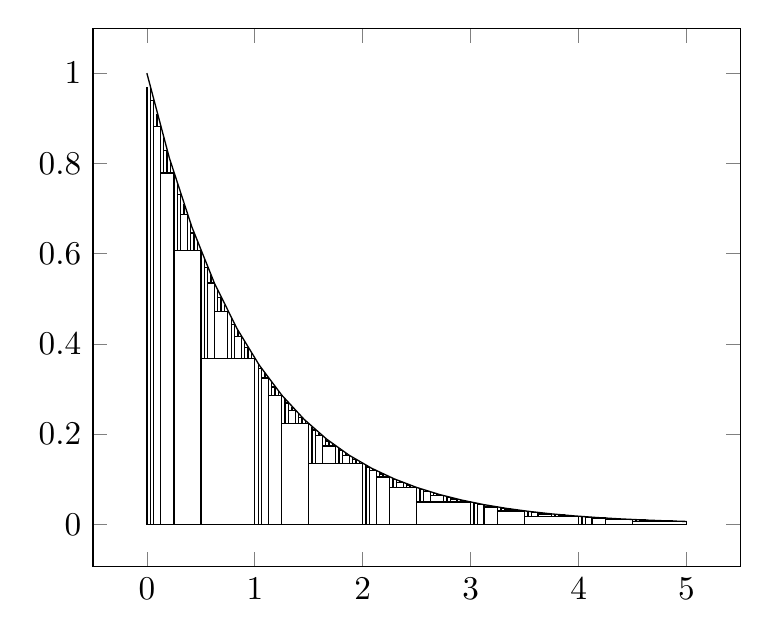
\begin{tikzpicture}[scale=1.2]
\begin{axis}
\addplot[domain=0:5] {e^(-x)};
\draw (axis cs: 0, 0) -- (axis cs: 5, 0);
\draw (axis cs: 0, 0) -- (axis cs: 0, 0.36787944160372466);
\draw (axis cs: 1, 0) -- (axis cs: 1, 0.36787944160372466);
\draw (axis cs: 0, 0) -- (axis cs: 0, 0.6065306600659573);
\draw (axis cs: 1/2, 0) -- (axis cs: 1/2, 0.6065306600659573);
\draw (axis cs: 1/2, 0) -- (axis cs: 1/2, 0.36787944182176296);
\draw (axis cs: 1, 0) -- (axis cs: 1, 0.36787944182176296);
\draw (axis cs: 1/2, 0.36787944182176296) -- (axis cs: 1, 0.36787944182176296);
\draw (axis cs: 0, 0) -- (axis cs: 0, 0.7788007832943493);
\draw (axis cs: 1/4, 0) -- (axis cs: 1/4, 0.7788007832943493);
\draw (axis cs: 1/4, 0) -- (axis cs: 1/4, 0.6065306602487321);
\draw (axis cs: 1/2, 0) -- (axis cs: 1/2, 0.6065306602487321);
\draw (axis cs: 1/4, 0.6065306602487321) -- (axis cs: 1/2, 0.6065306602487321);
\draw (axis cs: 1/2, 0.36787944182176296) -- (axis cs: 1/2, 0.4723665534165668);
\draw (axis cs: 3/4, 0.36787944182176296) -- (axis cs: 3/4, 0.4723665534165668);
\draw (axis cs: 3/4, 0.36787944182176296) -- (axis cs: 3/4, 0.36787944165116493);
\draw (axis cs: 1, 0.36787944182176296) -- (axis cs: 1, 0.36787944165116493);
\draw (axis cs: 3/4, 0.36787944165116493) -- (axis cs: 1, 0.36787944165116493);
\draw (axis cs: 0, 0) -- (axis cs: 0, 0.8824969027064975);
\draw (axis cs: 1/8, 0) -- (axis cs: 1/8, 0.8824969027064975);
\draw (axis cs: 1/8, 0) -- (axis cs: 1/8, 0.7788007834155871);
\draw (axis cs: 1/4, 0) -- (axis cs: 1/4, 0.7788007834155871);
\draw (axis cs: 1/8, 0.7788007834155871) -- (axis cs: 1/4, 0.7788007834155871);
\draw (axis cs: 1/4, 0.6065306602487321) -- (axis cs: 1/4, 0.6872892792824334);
\draw (axis cs: 3/8, 0.6065306602487321) -- (axis cs: 3/8, 0.6872892792824334);
\draw (axis cs: 3/8, 0.6065306602487321) -- (axis cs: 3/8, 0.6065306601050652);
\draw (axis cs: 1/2, 0.6065306602487321) -- (axis cs: 1/2, 0.6065306601050652);
\draw (axis cs: 3/8, 0.6065306601050652) -- (axis cs: 1/2, 0.6065306601050652);
\draw (axis cs: 1/2, 0.36787944182176296) -- (axis cs: 1/2, 0.5352614291382933);
\draw (axis cs: 5/8, 0.36787944182176296) -- (axis cs: 5/8, 0.5352614291382933);
\draw (axis cs: 5/8, 0.36787944182176296) -- (axis cs: 5/8, 0.47236655326632526);
\draw (axis cs: 3/4, 0.36787944182176296) -- (axis cs: 3/4, 0.47236655326632526);
\draw (axis cs: 5/8, 0.47236655326632526) -- (axis cs: 3/4, 0.47236655326632526);
\draw (axis cs: 3/4, 0.36787944165116493) -- (axis cs: 3/4, 0.4168620200899856);
\draw (axis cs: 7/8, 0.36787944165116493) -- (axis cs: 7/8, 0.4168620200899856);
\draw (axis cs: 7/8, 0.36787944165116493) -- (axis cs: 7/8, 0.36787944186014293);
\draw (axis cs: 1, 0.36787944165116493) -- (axis cs: 1, 0.36787944186014293);
\draw (axis cs: 7/8, 0.36787944186014293) -- (axis cs: 1, 0.36787944186014293);
\draw (axis cs: 0, 0) -- (axis cs: 0, 0.9394130629417682);
\draw (axis cs: 1/16, 0) -- (axis cs: 1/16, 0.9394130629417682);
\draw (axis cs: 1/16, 0) -- (axis cs: 1/16, 0.8824969027796001);
\draw (axis cs: 1/8, 0) -- (axis cs: 1/8, 0.8824969027796001);
\draw (axis cs: 1/16, 0.8824969027796001) -- (axis cs: 1/8, 0.8824969027796001);
\draw (axis cs: 1/8, 0.7788007834155871) -- (axis cs: 1/8, 0.829029118476808);
\draw (axis cs: 3/16, 0.7788007834155871) -- (axis cs: 3/16, 0.829029118476808);
\draw (axis cs: 3/16, 0.7788007834155871) -- (axis cs: 3/16, 0.778800783319457);
\draw (axis cs: 1/4, 0.7788007834155871) -- (axis cs: 1/4, 0.778800783319457);
\draw (axis cs: 3/16, 0.778800783319457) -- (axis cs: 1/4, 0.778800783319457);
\draw (axis cs: 1/4, 0.6065306602487321) -- (axis cs: 1/4, 0.7316156293698852);
\draw (axis cs: 5/16, 0.6065306602487321) -- (axis cs: 5/16, 0.7316156293698852);
\draw (axis cs: 5/16, 0.6065306602487321) -- (axis cs: 5/16, 0.687289279169697);
\draw (axis cs: 3/8, 0.6065306602487321) -- (axis cs: 3/8, 0.687289279169697);
\draw (axis cs: 5/16, 0.687289279169697) -- (axis cs: 3/8, 0.687289279169697);
\draw (axis cs: 3/8, 0.6065306601050652) -- (axis cs: 3/8, 0.645648526743318);
\draw (axis cs: 7/16, 0.6065306601050652) -- (axis cs: 7/16, 0.645648526743318);
\draw (axis cs: 7/16, 0.6065306601050652) -- (axis cs: 7/16, 0.6065306602803711);
\draw (axis cs: 1/2, 0.6065306601050652) -- (axis cs: 1/2, 0.6065306602803711);
\draw (axis cs: 7/16, 0.6065306602803711) -- (axis cs: 1/2, 0.6065306602803711);
\draw (axis cs: 1/2, 0.36787944182176296) -- (axis cs: 1/2, 0.5697828252642633);
\draw (axis cs: 9/16, 0.36787944182176296) -- (axis cs: 9/16, 0.5697828252642633);
\draw (axis cs: 9/16, 0.36787944182176296) -- (axis cs: 9/16, 0.5352614289897776);
\draw (axis cs: 5/8, 0.36787944182176296) -- (axis cs: 5/8, 0.5352614289897776);
\draw (axis cs: 9/16, 0.5352614289897776) -- (axis cs: 5/8, 0.5352614289897776);
\draw (axis cs: 5/8, 0.47236655326632526) -- (axis cs: 5/8, 0.5028315783817777);
\draw (axis cs: 11/16, 0.47236655326632526) -- (axis cs: 11/16, 0.5028315783817777);
\draw (axis cs: 11/16, 0.47236655326632526) -- (axis cs: 11/16, 0.4723665534564358);
\draw (axis cs: 3/4, 0.47236655326632526) -- (axis cs: 3/4, 0.4723665534564358);
\draw (axis cs: 11/16, 0.4723665534564358) -- (axis cs: 3/4, 0.4723665534564358);
\draw (axis cs: 3/4, 0.36787944165116493) -- (axis cs: 3/4, 0.4437473107531558);
\draw (axis cs: 13/16, 0.36787944165116493) -- (axis cs: 13/16, 0.4437473107531558);
\draw (axis cs: 13/16, 0.36787944165116493) -- (axis cs: 13/16, 0.4168620203098653);
\draw (axis cs: 7/8, 0.36787944165116493) -- (axis cs: 7/8, 0.4168620203098653);
\draw (axis cs: 13/16, 0.4168620203098653) -- (axis cs: 7/8, 0.4168620203098653);
\draw (axis cs: 7/8, 0.36787944186014293) -- (axis cs: 7/8, 0.3916056272654166);
\draw (axis cs: 15/16, 0.36787944186014293) -- (axis cs: 15/16, 0.3916056272654166);
\draw (axis cs: 15/16, 0.36787944186014293) -- (axis cs: 15/16, 0.3678794417014049);
\draw (axis cs: 1, 0.36787944186014293) -- (axis cs: 1, 0.3678794417014049);
\draw (axis cs: 15/16, 0.3678794417014049) -- (axis cs: 1, 0.3678794417014049);
\draw (axis cs: 0, 0) -- (axis cs: 0, 0.9692332345425265);
\draw (axis cs: 1/32, 0) -- (axis cs: 1/32, 0.9692332345425265);
\draw (axis cs: 1/32, 0) -- (axis cs: 1/32, 0.9394130629133053);
\draw (axis cs: 1/16, 0) -- (axis cs: 1/16, 0.9394130629133053);
\draw (axis cs: 1/32, 0.9394130629133053) -- (axis cs: 1/16, 0.9394130629133053);
\draw (axis cs: 1/16, 0.8824969027796001) -- (axis cs: 1/16, 0.9105103615428042);
\draw (axis cs: 3/32, 0.8824969027796001) -- (axis cs: 3/32, 0.9105103615428042);
\draw (axis cs: 3/32, 0.8824969027796001) -- (axis cs: 3/32, 0.8824969027207229);
\draw (axis cs: 1/8, 0.8824969027796001) -- (axis cs: 1/8, 0.8824969027207229);
\draw (axis cs: 3/32, 0.8824969027207229) -- (axis cs: 1/8, 0.8824969027207229);
\draw (axis cs: 1/8, 0.7788007834155871) -- (axis cs: 1/8, 0.8553453275548334);
\draw (axis cs: 5/32, 0.7788007834155871) -- (axis cs: 5/32, 0.8553453275548334);
\draw (axis cs: 5/32, 0.7788007834155871) -- (axis cs: 5/32, 0.8290291184046698);
\draw (axis cs: 3/16, 0.7788007834155871) -- (axis cs: 3/16, 0.8290291184046698);
\draw (axis cs: 5/32, 0.8290291184046698) -- (axis cs: 3/16, 0.8290291184046698);
\draw (axis cs: 3/16, 0.778800783319457) -- (axis cs: 3/16, 0.8035225738813201);
\draw (axis cs: 7/32, 0.778800783319457) -- (axis cs: 7/32, 0.8035225738813201);
\draw (axis cs: 7/32, 0.778800783319457) -- (axis cs: 7/32, 0.7788007834358996);
\draw (axis cs: 1/4, 0.778800783319457) -- (axis cs: 1/4, 0.7788007834358996);
\draw (axis cs: 7/32, 0.7788007834358996) -- (axis cs: 1/4, 0.7788007834358996);
\draw (axis cs: 1/4, 0.6065306602487321) -- (axis cs: 1/4, 0.7548396023407801);
\draw (axis cs: 9/32, 0.6065306602487321) -- (axis cs: 9/32, 0.7548396023407801);
\draw (axis cs: 9/32, 0.6065306602487321) -- (axis cs: 9/32, 0.7316156292647287);
\draw (axis cs: 5/16, 0.6065306602487321) -- (axis cs: 5/16, 0.7316156292647287);
\draw (axis cs: 9/32, 0.7316156292647287) -- (axis cs: 5/16, 0.7316156292647287);
\draw (axis cs: 5/16, 0.687289279169697) -- (axis cs: 5/16, 0.7091061827235392);
\draw (axis cs: 11/32, 0.687289279169697) -- (axis cs: 11/32, 0.7091061827235392);
\draw (axis cs: 11/32, 0.687289279169697) -- (axis cs: 11/32, 0.687289279311438);
\draw (axis cs: 3/8, 0.687289279169697) -- (axis cs: 3/8, 0.687289279311438);
\draw (axis cs: 11/32, 0.687289279311438) -- (axis cs: 3/8, 0.687289279311438);
\draw (axis cs: 3/8, 0.6065306601050652) -- (axis cs: 3/8, 0.6661436112079405);
\draw (axis cs: 13/32, 0.6065306601050652) -- (axis cs: 13/32, 0.6661436112079405);
\draw (axis cs: 13/32, 0.6065306601050652) -- (axis cs: 13/32, 0.6456485269168244);
\draw (axis cs: 7/16, 0.6065306601050652) -- (axis cs: 7/16, 0.6456485269168244);
\draw (axis cs: 13/32, 0.6456485269168244) -- (axis cs: 7/16, 0.6456485269168244);
\draw (axis cs: 7/16, 0.6065306602803711) -- (axis cs: 7/16, 0.6257840100717663);
\draw (axis cs: 15/32, 0.6065306602803711) -- (axis cs: 15/32, 0.6257840100717663);
\draw (axis cs: 15/32, 0.6065306602803711) -- (axis cs: 15/32, 0.606530660146481);
\draw (axis cs: 1/2, 0.6065306602803711) -- (axis cs: 1/2, 0.606530660146481);
\draw (axis cs: 15/32, 0.606530660146481) -- (axis cs: 1/2, 0.606530660146481);
\draw (axis cs: 1/2, 0.36787944182176296) -- (axis cs: 1/2, 0.5878696735244751);
\draw (axis cs: 17/32, 0.36787944182176296) -- (axis cs: 17/32, 0.5878696735244751);
\draw (axis cs: 17/32, 0.36787944182176296) -- (axis cs: 17/32, 0.5697828251028737);
\draw (axis cs: 9/16, 0.36787944182176296) -- (axis cs: 9/16, 0.5697828251028737);
\draw (axis cs: 17/32, 0.5697828251028737) -- (axis cs: 9/16, 0.5697828251028737);
\draw (axis cs: 9/16, 0.5352614289897776) -- (axis cs: 9/16, 0.5522524505062694);
\draw (axis cs: 19/32, 0.5352614289897776) -- (axis cs: 19/32, 0.5522524505062694);
\draw (axis cs: 19/32, 0.5352614289897776) -- (axis cs: 19/32, 0.5352614291748428);
\draw (axis cs: 5/8, 0.5352614289897776) -- (axis cs: 5/8, 0.5352614291748428);
\draw (axis cs: 19/32, 0.5352614291748428) -- (axis cs: 5/8, 0.5352614291748428);
\draw (axis cs: 5/8, 0.47236655326632526) -- (axis cs: 5/8, 0.5187931662895634);
\draw (axis cs: 21/32, 0.47236655326632526) -- (axis cs: 21/32, 0.5187931662895634);
\draw (axis cs: 21/32, 0.47236655326632526) -- (axis cs: 21/32, 0.5028315785870574);
\draw (axis cs: 11/16, 0.47236655326632526) -- (axis cs: 11/16, 0.5028315785870574);
\draw (axis cs: 21/32, 0.5028315785870574) -- (axis cs: 11/16, 0.5028315785870574);
\draw (axis cs: 11/16, 0.4723665534564358) -- (axis cs: 11/16, 0.4873610773107796);
\draw (axis cs: 23/32, 0.4723665534564358) -- (axis cs: 23/32, 0.4873610773107796);
\draw (axis cs: 23/32, 0.4723665534564358) -- (axis cs: 23/32, 0.4723665533185145);
\draw (axis cs: 3/4, 0.4723665534564358) -- (axis cs: 3/4, 0.4723665533185145);
\draw (axis cs: 23/32, 0.4723665533185145) -- (axis cs: 3/4, 0.4723665533185145);
\draw (axis cs: 3/4, 0.36787944165116493) -- (axis cs: 3/4, 0.45783336231703897);
\draw (axis cs: 25/32, 0.36787944165116493) -- (axis cs: 25/32, 0.45783336231703897);
\draw (axis cs: 25/32, 0.36787944165116493) -- (axis cs: 25/32, 0.4437473105958565);
\draw (axis cs: 13/16, 0.36787944165116493) -- (axis cs: 13/16, 0.4437473105958565);
\draw (axis cs: 25/32, 0.4437473105958565) -- (axis cs: 13/16, 0.4437473105958565);
\draw (axis cs: 13/16, 0.4168620203098653) -- (axis cs: 13/16, 0.4300946411255604);
\draw (axis cs: 27/32, 0.4168620203098653) -- (axis cs: 27/32, 0.4300946411255604);
\draw (axis cs: 27/32, 0.4168620203098653) -- (axis cs: 27/32, 0.4168620201360424);
\draw (axis cs: 7/8, 0.4168620203098653) -- (axis cs: 7/8, 0.4168620201360424);
\draw (axis cs: 27/32, 0.4168620201360424) -- (axis cs: 7/8, 0.4168620201360424);
\draw (axis cs: 7/8, 0.36787944186014293) -- (axis cs: 7/8, 0.4040365240941731);
\draw (axis cs: 29/32, 0.36787944186014293) -- (axis cs: 29/32, 0.4040365240941731);
\draw (axis cs: 29/32, 0.36787944186014293) -- (axis cs: 29/32, 0.3916056270821371);
\draw (axis cs: 15/16, 0.36787944186014293) -- (axis cs: 15/16, 0.3916056270821371);
\draw (axis cs: 29/32, 0.3916056270821371) -- (axis cs: 15/16, 0.3916056270821371);
\draw (axis cs: 15/16, 0.3678794417014049) -- (axis cs: 15/16, 0.37955718856409554);
\draw (axis cs: 31/32, 0.3678794417014049) -- (axis cs: 31/32, 0.37955718856409554);
\draw (axis cs: 31/32, 0.3678794417014049) -- (axis cs: 31/32, 0.367879441900788);
\draw (axis cs: 1, 0.3678794417014049) -- (axis cs: 1, 0.367879441900788);
\draw (axis cs: 31/32, 0.367879441900788) -- (axis cs: 1, 0.367879441900788);
\draw (axis cs: 1, 0) -- (axis cs: 1, 0.1353352833956405);
\draw (axis cs: 2, 0) -- (axis cs: 2, 0.1353352833956405);
\draw (axis cs: 1, 0) -- (axis cs: 1, 0.22313016027841043);
\draw (axis cs: 3/2, 0) -- (axis cs: 3/2, 0.22313016027841043);
\draw (axis cs: 3/2, 0) -- (axis cs: 3/2, 0.1353352834758523);
\draw (axis cs: 2, 0) -- (axis cs: 2, 0.1353352834758523);
\draw (axis cs: 3/2, 0.1353352834758523) -- (axis cs: 2, 0.1353352834758523);
\draw (axis cs: 1, 0) -- (axis cs: 1, 0.28650479694220676);
\draw (axis cs: 5/4, 0) -- (axis cs: 5/4, 0.28650479694220676);
\draw (axis cs: 5/4, 0) -- (axis cs: 5/4, 0.22313016034564953);
\draw (axis cs: 3/2, 0) -- (axis cs: 3/2, 0.22313016034564953);
\draw (axis cs: 5/4, 0.22313016034564953) -- (axis cs: 3/2, 0.22313016034564953);
\draw (axis cs: 3/2, 0.1353352834758523) -- (axis cs: 3/2, 0.17377394369896684);
\draw (axis cs: 7/4, 0.1353352834758523) -- (axis cs: 7/4, 0.17377394369896684);
\draw (axis cs: 7/4, 0.1353352834758523) -- (axis cs: 7/4, 0.13533528341309278);
\draw (axis cs: 2, 0.1353352834758523) -- (axis cs: 2, 0.13533528341309278);
\draw (axis cs: 7/4, 0.13533528341309278) -- (axis cs: 2, 0.13533528341309278);
\draw (axis cs: 1, 0) -- (axis cs: 1, 0.324652467403195);
\draw (axis cs: 9/8, 0) -- (axis cs: 9/8, 0.324652467403195);
\draw (axis cs: 9/8, 0) -- (axis cs: 9/8, 0.28650479698680764);
\draw (axis cs: 5/4, 0) -- (axis cs: 5/4, 0.28650479698680764);
\draw (axis cs: 9/8, 0.28650479698680764) -- (axis cs: 5/4, 0.28650479698680764);
\draw (axis cs: 5/4, 0.22313016034564953) -- (axis cs: 5/4, 0.252839595985545);
\draw (axis cs: 11/8, 0.22313016034564953) -- (axis cs: 11/8, 0.252839595985545);
\draw (axis cs: 11/8, 0.22313016034564953) -- (axis cs: 11/8, 0.22313016029279742);
\draw (axis cs: 3/2, 0.22313016034564953) -- (axis cs: 3/2, 0.22313016029279742);
\draw (axis cs: 11/8, 0.22313016029279742) -- (axis cs: 3/2, 0.22313016029279742);
\draw (axis cs: 3/2, 0.1353352834758523) -- (axis cs: 3/2, 0.19691167543202293);
\draw (axis cs: 13/8, 0.1353352834758523) -- (axis cs: 13/8, 0.19691167543202293);
\draw (axis cs: 13/8, 0.1353352834758523) -- (axis cs: 13/8, 0.17377394364369608);
\draw (axis cs: 7/4, 0.1353352834758523) -- (axis cs: 7/4, 0.17377394364369608);
\draw (axis cs: 13/8, 0.17377394364369608) -- (axis cs: 7/4, 0.17377394364369608);
\draw (axis cs: 7/4, 0.13533528341309278) -- (axis cs: 7/4, 0.15335496699630247);
\draw (axis cs: 15/8, 0.13533528341309278) -- (axis cs: 15/8, 0.15335496699630247);
\draw (axis cs: 15/8, 0.13533528341309278) -- (axis cs: 15/8, 0.1353352834899715);
\draw (axis cs: 2, 0.13533528341309278) -- (axis cs: 2, 0.1353352834899715);
\draw (axis cs: 15/8, 0.1353352834899715) -- (axis cs: 2, 0.1353352834899715);
\draw (axis cs: 1, 0) -- (axis cs: 1, 0.34559075262417066);
\draw (axis cs: 17/16, 0) -- (axis cs: 17/16, 0.34559075262417066);
\draw (axis cs: 17/16, 0) -- (axis cs: 17/16, 0.324652467430088);
\draw (axis cs: 9/8, 0) -- (axis cs: 9/8, 0.324652467430088);
\draw (axis cs: 17/16, 0.324652467430088) -- (axis cs: 9/8, 0.324652467430088);
\draw (axis cs: 9/8, 0.28650479698680764) -- (axis cs: 9/8, 0.3049827688201016);
\draw (axis cs: 19/16, 0.28650479698680764) -- (axis cs: 19/16, 0.3049827688201016);
\draw (axis cs: 19/16, 0.28650479698680764) -- (axis cs: 19/16, 0.2865047969514434);
\draw (axis cs: 5/4, 0.28650479698680764) -- (axis cs: 5/4, 0.2865047969514434);
\draw (axis cs: 19/16, 0.2865047969514434) -- (axis cs: 5/4, 0.2865047969514434);
\draw (axis cs: 5/4, 0.22313016034564953) -- (axis cs: 5/4, 0.2691463488848865);
\draw (axis cs: 21/16, 0.22313016034564953) -- (axis cs: 21/16, 0.2691463488848865);
\draw (axis cs: 21/16, 0.22313016034564953) -- (axis cs: 21/16, 0.2528395959440715);
\draw (axis cs: 11/8, 0.22313016034564953) -- (axis cs: 11/8, 0.2528395959440715);
\draw (axis cs: 21/16, 0.2528395959440715) -- (axis cs: 11/8, 0.2528395959440715);
\draw (axis cs: 11/8, 0.22313016029279742) -- (axis cs: 11/8, 0.23752081921149684);
\draw (axis cs: 23/16, 0.22313016029279742) -- (axis cs: 23/16, 0.23752081921149684);
\draw (axis cs: 23/16, 0.22313016029279742) -- (axis cs: 23/16, 0.22313016035728886);
\draw (axis cs: 3/2, 0.22313016029279742) -- (axis cs: 3/2, 0.22313016035728886);
\draw (axis cs: 23/16, 0.22313016035728886) -- (axis cs: 3/2, 0.22313016035728886);
\draw (axis cs: 3/2, 0.1353352834758523) -- (axis cs: 3/2, 0.20961138734730272);
\draw (axis cs: 25/16, 0.1353352834758523) -- (axis cs: 25/16, 0.20961138734730272);
\draw (axis cs: 25/16, 0.1353352834758523) -- (axis cs: 25/16, 0.19691167537738702);
\draw (axis cs: 13/8, 0.1353352834758523) -- (axis cs: 13/8, 0.19691167537738702);
\draw (axis cs: 25/16, 0.19691167537738702) -- (axis cs: 13/8, 0.19691167537738702);
\draw (axis cs: 13/8, 0.17377394364369608) -- (axis cs: 13/8, 0.18498140005844269);
\draw (axis cs: 27/16, 0.17377394364369608) -- (axis cs: 27/16, 0.18498140005844269);
\draw (axis cs: 27/16, 0.17377394364369608) -- (axis cs: 27/16, 0.17377394371363383);
\draw (axis cs: 7/4, 0.17377394364369608) -- (axis cs: 7/4, 0.17377394371363383);
\draw (axis cs: 27/16, 0.17377394371363383) -- (axis cs: 7/4, 0.17377394371363383);
\draw (axis cs: 7/4, 0.13533528341309278) -- (axis cs: 7/4, 0.16324551270120133);
\draw (axis cs: 29/16, 0.13533528341309278) -- (axis cs: 29/16, 0.16324551270120133);
\draw (axis cs: 29/16, 0.13533528341309278) -- (axis cs: 29/16, 0.15335496707719168);
\draw (axis cs: 15/8, 0.13533528341309278) -- (axis cs: 15/8, 0.15335496707719168);
\draw (axis cs: 29/16, 0.15335496707719168) -- (axis cs: 15/8, 0.15335496707719168);
\draw (axis cs: 15/8, 0.1353352834899715) -- (axis cs: 15/8, 0.1440636593179936);
\draw (axis cs: 31/16, 0.1353352834899715) -- (axis cs: 31/16, 0.1440636593179936);
\draw (axis cs: 31/16, 0.1353352834899715) -- (axis cs: 31/16, 0.13533528343157503);
\draw (axis cs: 2, 0.1353352834899715) -- (axis cs: 2, 0.13533528343157503);
\draw (axis cs: 31/16, 0.13533528343157503) -- (axis cs: 2, 0.13533528343157503);
\draw (axis cs: 1, 0) -- (axis cs: 1, 0.35656098068829417);
\draw (axis cs: 33/32, 0) -- (axis cs: 33/32, 0.35656098068829417);
\draw (axis cs: 33/32, 0) -- (axis cs: 33/32, 0.3455907526136997);
\draw (axis cs: 17/16, 0) -- (axis cs: 17/16, 0.3455907526136997);
\draw (axis cs: 33/32, 0.3455907526136997) -- (axis cs: 17/16, 0.3455907526136997);
\draw (axis cs: 17/16, 0.324652467430088) -- (axis cs: 17/16, 0.3349580429851747);
\draw (axis cs: 35/32, 0.324652467430088) -- (axis cs: 35/32, 0.3349580429851747);
\draw (axis cs: 35/32, 0.324652467430088) -- (axis cs: 35/32, 0.32465246740842824);
\draw (axis cs: 9/8, 0.324652467430088) -- (axis cs: 9/8, 0.32465246740842824);
\draw (axis cs: 35/32, 0.32465246740842824) -- (axis cs: 9/8, 0.32465246740842824);
\draw (axis cs: 9/8, 0.28650479698680764) -- (axis cs: 9/8, 0.3146639611094764);
\draw (axis cs: 37/32, 0.28650479698680764) -- (axis cs: 37/32, 0.3146639611094764);
\draw (axis cs: 37/32, 0.28650479698680764) -- (axis cs: 37/32, 0.3049827687935634);
\draw (axis cs: 19/16, 0.28650479698680764) -- (axis cs: 19/16, 0.3049827687935634);
\draw (axis cs: 37/32, 0.3049827687935634) -- (axis cs: 19/16, 0.3049827687935634);
\draw (axis cs: 19/16, 0.2865047969514434) -- (axis cs: 19/16, 0.295599435448099);
\draw (axis cs: 39/32, 0.2865047969514434) -- (axis cs: 39/32, 0.295599435448099);
\draw (axis cs: 39/32, 0.2865047969514434) -- (axis cs: 39/32, 0.2865047969942802);
\draw (axis cs: 5/4, 0.2865047969514434) -- (axis cs: 5/4, 0.2865047969942802);
\draw (axis cs: 39/32, 0.2865047969942802) -- (axis cs: 5/4, 0.2865047969942802);
\draw (axis cs: 5/4, 0.22313016034564953) -- (axis cs: 5/4, 0.2776899710831999);
\draw (axis cs: 41/32, 0.22313016034564953) -- (axis cs: 41/32, 0.2776899710831999);
\draw (axis cs: 41/32, 0.22313016034564953) -- (axis cs: 41/32, 0.2691463488462015);
\draw (axis cs: 21/16, 0.22313016034564953) -- (axis cs: 21/16, 0.2691463488462015);
\draw (axis cs: 41/32, 0.2691463488462015) -- (axis cs: 21/16, 0.2691463488462015);
\draw (axis cs: 21/16, 0.2528395959440715) -- (axis cs: 21/16, 0.26086558623155026);
\draw (axis cs: 43/32, 0.2528395959440715) -- (axis cs: 43/32, 0.26086558623155026);
\draw (axis cs: 43/32, 0.2528395959440715) -- (axis cs: 43/32, 0.2528395959962152);
\draw (axis cs: 11/8, 0.2528395959440715) -- (axis cs: 11/8, 0.2528395959962152);
\draw (axis cs: 43/32, 0.2528395959962152) -- (axis cs: 11/8, 0.2528395959962152);
\draw (axis cs: 11/8, 0.22313016029279742) -- (axis cs: 11/8, 0.24506053943110373);
\draw (axis cs: 45/32, 0.22313016029279742) -- (axis cs: 45/32, 0.24506053943110373);
\draw (axis cs: 45/32, 0.22313016029279742) -- (axis cs: 45/32, 0.2375208192753263);
\draw (axis cs: 23/16, 0.22313016029279742) -- (axis cs: 23/16, 0.2375208192753263);
\draw (axis cs: 45/32, 0.2375208192753263) -- (axis cs: 23/16, 0.2375208192753263);
\draw (axis cs: 23/16, 0.22313016035728886) -- (axis cs: 23/16, 0.2302130719192256);
\draw (axis cs: 47/32, 0.22313016035728886) -- (axis cs: 47/32, 0.2302130719192256);
\draw (axis cs: 47/32, 0.22313016035728886) -- (axis cs: 47/32, 0.22313016030803345);
\draw (axis cs: 3/2, 0.22313016035728886) -- (axis cs: 3/2, 0.22313016030803345);
\draw (axis cs: 47/32, 0.22313016030803345) -- (axis cs: 3/2, 0.22313016030803345);
\draw (axis cs: 3/2, 0.1353352834758523) -- (axis cs: 3/2, 0.2162651669778221);
\draw (axis cs: 49/32, 0.1353352834758523) -- (axis cs: 49/32, 0.2162651669778221);
\draw (axis cs: 49/32, 0.1353352834758523) -- (axis cs: 49/32, 0.20961138728793083);
\draw (axis cs: 25/16, 0.1353352834758523) -- (axis cs: 25/16, 0.20961138728793083);
\draw (axis cs: 49/32, 0.20961138728793083) -- (axis cs: 25/16, 0.20961138728793083);
\draw (axis cs: 25/16, 0.19691167537738702) -- (axis cs: 25/16, 0.203162322877806);
\draw (axis cs: 51/32, 0.19691167537738702) -- (axis cs: 51/32, 0.203162322877806);
\draw (axis cs: 51/32, 0.19691167537738702) -- (axis cs: 51/32, 0.19691167544546867);
\draw (axis cs: 13/8, 0.19691167537738702) -- (axis cs: 13/8, 0.19691167544546867);
\draw (axis cs: 51/32, 0.19691167544546867) -- (axis cs: 13/8, 0.19691167544546867);
\draw (axis cs: 13/8, 0.17377394364369608) -- (axis cs: 13/8, 0.1908533400981677);
\draw (axis cs: 53/32, 0.17377394364369608) -- (axis cs: 53/32, 0.1908533400981677);
\draw (axis cs: 53/32, 0.17377394364369608) -- (axis cs: 53/32, 0.18498140013396083);
\draw (axis cs: 27/16, 0.17377394364369608) -- (axis cs: 27/16, 0.18498140013396083);
\draw (axis cs: 53/32, 0.18498140013396083) -- (axis cs: 27/16, 0.18498140013396083);
\draw (axis cs: 27/16, 0.17377394371363383) -- (axis cs: 27/16, 0.17929012076980166);
\draw (axis cs: 55/32, 0.17377394371363383) -- (axis cs: 55/32, 0.17929012076980166);
\draw (axis cs: 55/32, 0.17377394371363383) -- (axis cs: 55/32, 0.1737739436628954);
\draw (axis cs: 7/4, 0.17377394371363383) -- (axis cs: 7/4, 0.1737739436628954);
\draw (axis cs: 55/32, 0.1737739436628954) -- (axis cs: 7/4, 0.1737739436628954);
\draw (axis cs: 7/4, 0.13533528341309278) -- (axis cs: 7/4, 0.16842748147883477);
\draw (axis cs: 57/32, 0.13533528341309278) -- (axis cs: 57/32, 0.16842748147883477);
\draw (axis cs: 57/32, 0.13533528341309278) -- (axis cs: 57/32, 0.16324551264333415);
\draw (axis cs: 29/16, 0.13533528341309278) -- (axis cs: 29/16, 0.16324551264333415);
\draw (axis cs: 57/32, 0.16324551264333415) -- (axis cs: 29/16, 0.16324551264333415);
\draw (axis cs: 29/16, 0.15335496707719168) -- (axis cs: 29/16, 0.1582229762281032);
\draw (axis cs: 59/32, 0.15335496707719168) -- (axis cs: 59/32, 0.1582229762281032);
\draw (axis cs: 59/32, 0.15335496707719168) -- (axis cs: 59/32, 0.1533549670132458);
\draw (axis cs: 15/8, 0.15335496707719168) -- (axis cs: 15/8, 0.1533549670132458);
\draw (axis cs: 59/32, 0.1533549670132458) -- (axis cs: 15/8, 0.1533549670132458);
\draw (axis cs: 15/8, 0.1353352834899715) -- (axis cs: 15/8, 0.1486367306966164);
\draw (axis cs: 61/32, 0.1353352834899715) -- (axis cs: 61/32, 0.1486367306966164);
\draw (axis cs: 61/32, 0.1353352834899715) -- (axis cs: 61/32, 0.14406365925056883);
\draw (axis cs: 31/16, 0.1353352834899715) -- (axis cs: 31/16, 0.14406365925056883);
\draw (axis cs: 61/32, 0.14406365925056883) -- (axis cs: 31/16, 0.14406365925056883);
\draw (axis cs: 31/16, 0.13533528343157503) -- (axis cs: 31/16, 0.13963128642156322);
\draw (axis cs: 63/32, 0.13533528343157503) -- (axis cs: 63/32, 0.13963128642156322);
\draw (axis cs: 63/32, 0.13533528343157503) -- (axis cs: 63/32, 0.13533528350492396);
\draw (axis cs: 2, 0.13533528343157503) -- (axis cs: 2, 0.13533528350492396);
\draw (axis cs: 63/32, 0.13533528350492396) -- (axis cs: 2, 0.13533528350492396);
\draw (axis cs: 2, 0) -- (axis cs: 2, 0.049787068426367);
\draw (axis cs: 3, 0) -- (axis cs: 3, 0.049787068426367);
\draw (axis cs: 2, 0) -- (axis cs: 2, 0.082084998671716);
\draw (axis cs: 5/2, 0) -- (axis cs: 5/2, 0.082084998671716);
\draw (axis cs: 5/2, 0) -- (axis cs: 5/2, 0.04978706845587527);
\draw (axis cs: 3, 0) -- (axis cs: 3, 0.04978706845587527);
\draw (axis cs: 5/2, 0.04978706845587527) -- (axis cs: 3, 0.04978706845587527);
\draw (axis cs: 2, 0) -- (axis cs: 2, 0.10539922459203656);
\draw (axis cs: 9/4, 0) -- (axis cs: 9/4, 0.10539922459203656);
\draw (axis cs: 9/4, 0) -- (axis cs: 9/4, 0.08208499869645187);
\draw (axis cs: 5/2, 0) -- (axis cs: 5/2, 0.08208499869645187);
\draw (axis cs: 9/4, 0.08208499869645187) -- (axis cs: 5/2, 0.08208499869645187);
\draw (axis cs: 5/2, 0.04978706845587527) -- (axis cs: 5/2, 0.06392786129813362);
\draw (axis cs: 11/4, 0.04978706845587527) -- (axis cs: 11/4, 0.06392786129813362);
\draw (axis cs: 11/4, 0.04978706845587527) -- (axis cs: 11/4, 0.049787068432787344);
\draw (axis cs: 3, 0.04978706845587527) -- (axis cs: 3, 0.049787068432787344);
\draw (axis cs: 11/4, 0.049787068432787344) -- (axis cs: 3, 0.049787068432787344);
\draw (axis cs: 2, 0) -- (axis cs: 2, 0.11943296828321726);
\draw (axis cs: 17/8, 0) -- (axis cs: 17/8, 0.11943296828321726);
\draw (axis cs: 17/8, 0) -- (axis cs: 17/8, 0.10539922460844436);
\draw (axis cs: 9/4, 0) -- (axis cs: 9/4, 0.10539922460844436);
\draw (axis cs: 17/8, 0.10539922460844436) -- (axis cs: 9/4, 0.10539922460844436);
\draw (axis cs: 9/4, 0.08208499869645187) -- (axis cs: 9/4, 0.09301448927717554);
\draw (axis cs: 19/8, 0.08208499869645187) -- (axis cs: 19/8, 0.09301448927717554);
\draw (axis cs: 19/8, 0.08208499869645187) -- (axis cs: 19/8, 0.08208499867700865);
\draw (axis cs: 5/2, 0.08208499869645187) -- (axis cs: 5/2, 0.08208499867700865);
\draw (axis cs: 19/8, 0.08208499867700865) -- (axis cs: 5/2, 0.08208499867700865);
\draw (axis cs: 5/2, 0.04978706845587527) -- (axis cs: 5/2, 0.07243975711806502);
\draw (axis cs: 21/8, 0.04978706845587527) -- (axis cs: 21/8, 0.07243975711806502);
\draw (axis cs: 21/8, 0.04978706845587527) -- (axis cs: 21/8, 0.06392786127780062);
\draw (axis cs: 11/4, 0.04978706845587527) -- (axis cs: 11/4, 0.06392786127780062);
\draw (axis cs: 21/8, 0.06392786127780062) -- (axis cs: 11/4, 0.06392786127780062);
\draw (axis cs: 11/4, 0.049787068432787344) -- (axis cs: 11/4, 0.05641613955946473);
\draw (axis cs: 23/8, 0.049787068432787344) -- (axis cs: 23/8, 0.05641613955946473);
\draw (axis cs: 23/8, 0.049787068432787344) -- (axis cs: 23/8, 0.04978706846106944);
\draw (axis cs: 3, 0.049787068432787344) -- (axis cs: 3, 0.04978706846106944);
\draw (axis cs: 23/8, 0.04978706846106944) -- (axis cs: 3, 0.04978706846106944);
\draw (axis cs: 2, 0) -- (axis cs: 2, 0.1271357329493981);
\draw (axis cs: 33/16, 0) -- (axis cs: 33/16, 0.1271357329493981);
\draw (axis cs: 33/16, 0) -- (axis cs: 33/16, 0.11943296829311066);
\draw (axis cs: 17/8, 0) -- (axis cs: 17/8, 0.11943296829311066);
\draw (axis cs: 33/16, 0.11943296829311066) -- (axis cs: 17/8, 0.11943296829311066);
\draw (axis cs: 17/8, 0.10539922460844436) -- (axis cs: 17/8, 0.11219689056045815);
\draw (axis cs: 35/16, 0.10539922460844436) -- (axis cs: 35/16, 0.11219689056045815);
\draw (axis cs: 35/16, 0.10539922460844436) -- (axis cs: 35/16, 0.10539922459543453);
\draw (axis cs: 9/4, 0.10539922460844436) -- (axis cs: 9/4, 0.10539922459543453);
\draw (axis cs: 35/16, 0.10539922459543453) -- (axis cs: 9/4, 0.10539922459543453);
\draw (axis cs: 9/4, 0.08208499869645187) -- (axis cs: 9/4, 0.09901340842110608);
\draw (axis cs: 37/16, 0.08208499869645187) -- (axis cs: 37/16, 0.09901340842110608);
\draw (axis cs: 37/16, 0.08208499869645187) -- (axis cs: 37/16, 0.09301448926191828);
\draw (axis cs: 19/8, 0.08208499869645187) -- (axis cs: 19/8, 0.09301448926191828);
\draw (axis cs: 37/16, 0.09301448926191828) -- (axis cs: 19/8, 0.09301448926191828);
\draw (axis cs: 19/8, 0.08208499867700865) -- (axis cs: 19/8, 0.08737902623810864);
\draw (axis cs: 39/16, 0.08208499867700865) -- (axis cs: 39/16, 0.08737902623810864);
\draw (axis cs: 39/16, 0.08208499867700865) -- (axis cs: 39/16, 0.08208499870073373);
\draw (axis cs: 5/2, 0.08208499867700865) -- (axis cs: 5/2, 0.08208499870073373);
\draw (axis cs: 39/16, 0.08208499870073373) -- (axis cs: 5/2, 0.08208499870073373);
\draw (axis cs: 5/2, 0.04978706845587527) -- (axis cs: 5/2, 0.07711172004049648);
\draw (axis cs: 41/16, 0.04978706845587527) -- (axis cs: 41/16, 0.07711172004049648);
\draw (axis cs: 41/16, 0.04978706845587527) -- (axis cs: 41/16, 0.07243975709796557);
\draw (axis cs: 21/8, 0.04978706845587527) -- (axis cs: 21/8, 0.07243975709796557);
\draw (axis cs: 41/16, 0.07243975709796557) -- (axis cs: 21/8, 0.07243975709796557);
\draw (axis cs: 21/8, 0.06392786127780062) -- (axis cs: 21/8, 0.0680508540806109);
\draw (axis cs: 43/16, 0.06392786127780062) -- (axis cs: 43/16, 0.0680508540806109);
\draw (axis cs: 43/16, 0.06392786127780062) -- (axis cs: 43/16, 0.0639278613035293);
\draw (axis cs: 11/4, 0.06392786127780062) -- (axis cs: 11/4, 0.0639278613035293);
\draw (axis cs: 43/16, 0.0639278613035293) -- (axis cs: 11/4, 0.0639278613035293);
\draw (axis cs: 11/4, 0.049787068432787344) -- (axis cs: 11/4, 0.06005466798626354);
\draw (axis cs: 45/16, 0.049787068432787344) -- (axis cs: 45/16, 0.06005466798626354);
\draw (axis cs: 45/16, 0.049787068432787344) -- (axis cs: 45/16, 0.056416139589222224);
\draw (axis cs: 23/8, 0.049787068432787344) -- (axis cs: 23/8, 0.056416139589222224);
\draw (axis cs: 45/16, 0.056416139589222224) -- (axis cs: 23/8, 0.056416139589222224);
\draw (axis cs: 23/8, 0.04978706846106944) -- (axis cs: 23/8, 0.052998058483016516);
\draw (axis cs: 47/16, 0.04978706846106944) -- (axis cs: 47/16, 0.052998058483016516);
\draw (axis cs: 47/16, 0.04978706846106944) -- (axis cs: 47/16, 0.04978706843958658);
\draw (axis cs: 3, 0.04978706846106944) -- (axis cs: 3, 0.04978706843958658);
\draw (axis cs: 47/16, 0.04978706843958658) -- (axis cs: 3, 0.04978706843958658);
\draw (axis cs: 2, 0) -- (axis cs: 2, 0.13117145431915106);
\draw (axis cs: 65/32, 0) -- (axis cs: 65/32, 0.13117145431915106);
\draw (axis cs: 65/32, 0) -- (axis cs: 65/32, 0.12713573294554603);
\draw (axis cs: 33/16, 0) -- (axis cs: 33/16, 0.12713573294554603);
\draw (axis cs: 65/32, 0.12713573294554603) -- (axis cs: 33/16, 0.12713573294554603);
\draw (axis cs: 33/16, 0.11943296829311066) -- (axis cs: 33/16, 0.12322417766926605);
\draw (axis cs: 67/32, 0.11943296829311066) -- (axis cs: 67/32, 0.12322417766926605);
\draw (axis cs: 67/32, 0.11943296829311066) -- (axis cs: 67/32, 0.11943296828514247);
\draw (axis cs: 17/8, 0.11943296829311066) -- (axis cs: 17/8, 0.11943296828514247);
\draw (axis cs: 67/32, 0.11943296828514247) -- (axis cs: 17/8, 0.11943296828514247);
\draw (axis cs: 17/8, 0.10539922460844436) -- (axis cs: 17/8, 0.11575840216974664);
\draw (axis cs: 69/32, 0.10539922460844436) -- (axis cs: 69/32, 0.11575840216974664);
\draw (axis cs: 69/32, 0.10539922460844436) -- (axis cs: 69/32, 0.11219689055069529);
\draw (axis cs: 35/16, 0.10539922460844436) -- (axis cs: 35/16, 0.11219689055069529);
\draw (axis cs: 69/32, 0.11219689055069529) -- (axis cs: 35/16, 0.11219689055069529);
\draw (axis cs: 35/16, 0.10539922459543453) -- (axis cs: 35/16, 0.10874495512324052);
\draw (axis cs: 71/32, 0.10539922459543453) -- (axis cs: 71/32, 0.10874495512324052);
\draw (axis cs: 71/32, 0.10539922459543453) -- (axis cs: 71/32, 0.10539922461119336);
\draw (axis cs: 9/4, 0.10539922459543453) -- (axis cs: 9/4, 0.10539922461119336);
\draw (axis cs: 71/32, 0.10539922461119336) -- (axis cs: 9/4, 0.10539922461119336);
\draw (axis cs: 9/4, 0.08208499869645187) -- (axis cs: 9/4, 0.10215643138100157);
\draw (axis cs: 73/32, 0.08208499869645187) -- (axis cs: 73/32, 0.10215643138100157);
\draw (axis cs: 73/32, 0.08208499869645187) -- (axis cs: 73/32, 0.09901340840687467);
\draw (axis cs: 37/16, 0.08208499869645187) -- (axis cs: 37/16, 0.09901340840687467);
\draw (axis cs: 73/32, 0.09901340840687467) -- (axis cs: 37/16, 0.09901340840687467);
\draw (axis cs: 37/16, 0.09301448926191828) -- (axis cs: 37/16, 0.09596708608372344);
\draw (axis cs: 75/32, 0.09301448926191828) -- (axis cs: 75/32, 0.09596708608372344);
\draw (axis cs: 75/32, 0.09301448926191828) -- (axis cs: 75/32, 0.09301448928110088);
\draw (axis cs: 19/8, 0.09301448926191828) -- (axis cs: 19/8, 0.09301448928110088);
\draw (axis cs: 75/32, 0.09301448928110088) -- (axis cs: 19/8, 0.09301448928110088);
\draw (axis cs: 19/8, 0.08208499867700865) -- (axis cs: 19/8, 0.09015273429908664);
\draw (axis cs: 77/32, 0.08208499867700865) -- (axis cs: 77/32, 0.09015273429908664);
\draw (axis cs: 77/32, 0.08208499867700865) -- (axis cs: 77/32, 0.08737902626159019);
\draw (axis cs: 39/16, 0.08208499867700865) -- (axis cs: 39/16, 0.08737902626159019);
\draw (axis cs: 77/32, 0.08737902626159019) -- (axis cs: 39/16, 0.08737902626159019);
\draw (axis cs: 39/16, 0.08208499870073373) -- (axis cs: 39/16, 0.08469065624800577);
\draw (axis cs: 79/32, 0.08208499870073373) -- (axis cs: 79/32, 0.08469065624800577);
\draw (axis cs: 79/32, 0.08208499870073373) -- (axis cs: 79/32, 0.08208499868261367);
\draw (axis cs: 5/2, 0.08208499870073373) -- (axis cs: 5/2, 0.08208499868261367);
\draw (axis cs: 79/32, 0.08208499868261367) -- (axis cs: 5/2, 0.08208499868261367);
\draw (axis cs: 5/2, 0.04978706845587527) -- (axis cs: 5/2, 0.07955950877264988);
\draw (axis cs: 81/32, 0.04978706845587527) -- (axis cs: 81/32, 0.07955950877264988);
\draw (axis cs: 81/32, 0.04978706845587527) -- (axis cs: 81/32, 0.07711172001865477);
\draw (axis cs: 41/16, 0.04978706845587527) -- (axis cs: 41/16, 0.07711172001865477);
\draw (axis cs: 81/32, 0.07711172001865477) -- (axis cs: 41/16, 0.07711172001865477);
\draw (axis cs: 41/16, 0.07243975709796557) -- (axis cs: 41/16, 0.0747392418073794);
\draw (axis cs: 83/32, 0.07243975709796557) -- (axis cs: 83/32, 0.0747392418073794);
\draw (axis cs: 83/32, 0.07243975709796557) -- (axis cs: 83/32, 0.07243975712301144);
\draw (axis cs: 21/8, 0.07243975709796557) -- (axis cs: 21/8, 0.07243975712301144);
\draw (axis cs: 83/32, 0.07243975712301144) -- (axis cs: 21/8, 0.07243975712301144);
\draw (axis cs: 21/8, 0.06392786127780062) -- (axis cs: 21/8, 0.07021102010101717);
\draw (axis cs: 85/32, 0.06392786127780062) -- (axis cs: 85/32, 0.07021102010101717);
\draw (axis cs: 85/32, 0.06392786127780062) -- (axis cs: 85/32, 0.06805085410839247);
\draw (axis cs: 43/16, 0.06392786127780062) -- (axis cs: 43/16, 0.06805085410839247);
\draw (axis cs: 85/32, 0.06805085410839247) -- (axis cs: 43/16, 0.06805085410839247);
\draw (axis cs: 43/16, 0.0639278613035293) -- (axis cs: 43/16, 0.06595714943635504);
\draw (axis cs: 87/32, 0.0639278613035293) -- (axis cs: 87/32, 0.06595714943635504);
\draw (axis cs: 87/32, 0.0639278613035293) -- (axis cs: 87/32, 0.06392786128486366);
\draw (axis cs: 11/4, 0.0639278613035293) -- (axis cs: 11/4, 0.06392786128486366);
\draw (axis cs: 87/32, 0.06392786128486366) -- (axis cs: 11/4, 0.06392786128486366);
\draw (axis cs: 11/4, 0.049787068432787344) -- (axis cs: 11/4, 0.0619610077643472);
\draw (axis cs: 89/32, 0.049787068432787344) -- (axis cs: 89/32, 0.0619610077643472);
\draw (axis cs: 89/32, 0.049787068432787344) -- (axis cs: 89/32, 0.06005466796497539);
\draw (axis cs: 45/16, 0.049787068432787344) -- (axis cs: 45/16, 0.06005466796497539);
\draw (axis cs: 89/32, 0.06005466796497539) -- (axis cs: 45/16, 0.06005466796497539);
\draw (axis cs: 45/16, 0.056416139589222224) -- (axis cs: 45/16, 0.058206980075277005);
\draw (axis cs: 91/32, 0.056416139589222224) -- (axis cs: 91/32, 0.058206980075277005);
\draw (axis cs: 91/32, 0.056416139589222224) -- (axis cs: 91/32, 0.05641613956569784);
\draw (axis cs: 23/8, 0.056416139589222224) -- (axis cs: 23/8, 0.05641613956569784);
\draw (axis cs: 91/32, 0.05641613956569784) -- (axis cs: 23/8, 0.05641613956569784);
\draw (axis cs: 23/8, 0.04978706846106944) -- (axis cs: 23/8, 0.0546803974262214);
\draw (axis cs: 93/32, 0.04978706846106944) -- (axis cs: 93/32, 0.0546803974262214);
\draw (axis cs: 93/32, 0.04978706846106944) -- (axis cs: 93/32, 0.05299805845821235);
\draw (axis cs: 47/16, 0.04978706846106944) -- (axis cs: 47/16, 0.05299805845821235);
\draw (axis cs: 93/32, 0.05299805845821235) -- (axis cs: 47/16, 0.05299805845821235);
\draw (axis cs: 47/16, 0.04978706843958658) -- (axis cs: 47/16, 0.051367479618814285);
\draw (axis cs: 95/32, 0.04978706843958658) -- (axis cs: 95/32, 0.051367479618814285);
\draw (axis cs: 95/32, 0.04978706843958658) -- (axis cs: 95/32, 0.04978706846657014);
\draw (axis cs: 3, 0.04978706843958658) -- (axis cs: 3, 0.04978706846657014);
\draw (axis cs: 95/32, 0.04978706846657014) -- (axis cs: 3, 0.04978706846657014);
\draw (axis cs: 3, 0) -- (axis cs: 3, 0.018315638910256254);
\draw (axis cs: 4, 0) -- (axis cs: 4, 0.018315638910256254);
\draw (axis cs: 3, 0) -- (axis cs: 3, 0.030197383439909464);
\draw (axis cs: 7/2, 0) -- (axis cs: 7/2, 0.030197383439909464);
\draw (axis cs: 7/2, 0) -- (axis cs: 7/2, 0.01831563892111174);
\draw (axis cs: 4, 0) -- (axis cs: 4, 0.01831563892111174);
\draw (axis cs: 7/2, 0.01831563892111174) -- (axis cs: 4, 0.01831563892111174);
\draw (axis cs: 3, 0) -- (axis cs: 3, 0.038774207842821755);
\draw (axis cs: 13/4, 0) -- (axis cs: 13/4, 0.038774207842821755);
\draw (axis cs: 13/4, 0) -- (axis cs: 13/4, 0.030197383449009286);
\draw (axis cs: 7/2, 0) -- (axis cs: 7/2, 0.030197383449009286);
\draw (axis cs: 13/4, 0.030197383449009286) -- (axis cs: 7/2, 0.030197383449009286);
\draw (axis cs: 7/2, 0.01831563892111174) -- (axis cs: 7/2, 0.023517745889642873);
\draw (axis cs: 15/4, 0.01831563892111174) -- (axis cs: 15/4, 0.023517745889642873);
\draw (axis cs: 15/4, 0.01831563892111174) -- (axis cs: 15/4, 0.018315638912618164);
\draw (axis cs: 4, 0.01831563892111174) -- (axis cs: 4, 0.018315638912618164);
\draw (axis cs: 15/4, 0.018315638912618164) -- (axis cs: 4, 0.018315638912618164);
\draw (axis cs: 3, 0) -- (axis cs: 3, 0.04393693362947656);
\draw (axis cs: 25/8, 0) -- (axis cs: 25/8, 0.04393693362947656);
\draw (axis cs: 25/8, 0) -- (axis cs: 25/8, 0.03877420784885784);
\draw (axis cs: 13/4, 0) -- (axis cs: 13/4, 0.03877420784885784);
\draw (axis cs: 25/8, 0.03877420784885784) -- (axis cs: 13/4, 0.03877420784885784);
\draw (axis cs: 13/4, 0.030197383449009286) -- (axis cs: 13/4, 0.03421811833613445);
\draw (axis cs: 27/8, 0.030197383449009286) -- (axis cs: 27/8, 0.03421811833613445);
\draw (axis cs: 27/8, 0.030197383449009286) -- (axis cs: 27/8, 0.030197383441856525);
\draw (axis cs: 7/2, 0.030197383449009286) -- (axis cs: 7/2, 0.030197383441856525);
\draw (axis cs: 27/8, 0.030197383441856525) -- (axis cs: 7/2, 0.030197383441856525);
\draw (axis cs: 7/2, 0.01831563892111174) -- (axis cs: 7/2, 0.026649097367188773);
\draw (axis cs: 29/8, 0.01831563892111174) -- (axis cs: 29/8, 0.026649097367188773);
\draw (axis cs: 29/8, 0.01831563892111174) -- (axis cs: 29/8, 0.02351774588216278);
\draw (axis cs: 15/4, 0.01831563892111174) -- (axis cs: 15/4, 0.02351774588216278);
\draw (axis cs: 29/8, 0.02351774588216278) -- (axis cs: 15/4, 0.02351774588216278);
\draw (axis cs: 15/4, 0.018315638912618164) -- (axis cs: 15/4, 0.020754337894185983);
\draw (axis cs: 31/8, 0.018315638912618164) -- (axis cs: 31/8, 0.020754337894185983);
\draw (axis cs: 31/8, 0.018315638912618164) -- (axis cs: 31/8, 0.018315638923022567);
\draw (axis cs: 4, 0.018315638912618164) -- (axis cs: 4, 0.018315638923022567);
\draw (axis cs: 31/8, 0.018315638923022567) -- (axis cs: 4, 0.018315638923022567);
\draw (axis cs: 3, 0) -- (axis cs: 3, 0.046770622390346295);
\draw (axis cs: 49/16, 0) -- (axis cs: 49/16, 0.046770622390346295);
\draw (axis cs: 49/16, 0) -- (axis cs: 49/16, 0.04393693363311614);
\draw (axis cs: 25/8, 0) -- (axis cs: 25/8, 0.04393693363311614);
\draw (axis cs: 49/16, 0.04393693363311614) -- (axis cs: 25/8, 0.04393693363311614);
\draw (axis cs: 25/8, 0.03877420784885784) -- (axis cs: 25/8, 0.04127492940055481);
\draw (axis cs: 51/16, 0.03877420784885784) -- (axis cs: 51/16, 0.04127492940055481);
\draw (axis cs: 51/16, 0.03877420784885784) -- (axis cs: 51/16, 0.0387742078440718);
\draw (axis cs: 13/4, 0.03877420784885784) -- (axis cs: 13/4, 0.0387742078440718);
\draw (axis cs: 51/16, 0.0387742078440718) -- (axis cs: 13/4, 0.0387742078440718);
\draw (axis cs: 13/4, 0.030197383449009286) -- (axis cs: 13/4, 0.03642499735843629);
\draw (axis cs: 53/16, 0.030197383449009286) -- (axis cs: 53/16, 0.03642499735843629);
\draw (axis cs: 53/16, 0.030197383449009286) -- (axis cs: 53/16, 0.03421811833052162);
\draw (axis cs: 27/8, 0.030197383449009286) -- (axis cs: 27/8, 0.03421811833052162);
\draw (axis cs: 53/16, 0.03421811833052162) -- (axis cs: 27/8, 0.03421811833052162);
\draw (axis cs: 27/8, 0.030197383441856525) -- (axis cs: 27/8, 0.0321449473425802);
\draw (axis cs: 55/16, 0.030197383441856525) -- (axis cs: 55/16, 0.0321449473425802);
\draw (axis cs: 55/16, 0.030197383441856525) -- (axis cs: 55/16, 0.03019738345058449);
\draw (axis cs: 7/2, 0.030197383441856525) -- (axis cs: 7/2, 0.03019738345058449);
\draw (axis cs: 55/16, 0.03019738345058449) -- (axis cs: 7/2, 0.03019738345058449);
\draw (axis cs: 7/2, 0.01831563892111174) -- (axis cs: 7/2, 0.028367816476266555);
\draw (axis cs: 57/16, 0.01831563892111174) -- (axis cs: 57/16, 0.028367816476266555);
\draw (axis cs: 57/16, 0.01831563892111174) -- (axis cs: 57/16, 0.0266490973597946);
\draw (axis cs: 29/8, 0.01831563892111174) -- (axis cs: 29/8, 0.0266490973597946);
\draw (axis cs: 57/16, 0.0266490973597946) -- (axis cs: 29/8, 0.0266490973597946);
\draw (axis cs: 29/8, 0.02351774588216278) -- (axis cs: 29/8, 0.025034510170414505);
\draw (axis cs: 59/16, 0.02351774588216278) -- (axis cs: 59/16, 0.025034510170414505);
\draw (axis cs: 59/16, 0.02351774588216278) -- (axis cs: 59/16, 0.023517745891627834);
\draw (axis cs: 15/4, 0.02351774588216278) -- (axis cs: 15/4, 0.023517745891627834);
\draw (axis cs: 59/16, 0.023517745891627834) -- (axis cs: 15/4, 0.023517745891627834);
\draw (axis cs: 15/4, 0.018315638912618164) -- (axis cs: 15/4, 0.02209287769852314);
\draw (axis cs: 61/16, 0.018315638912618164) -- (axis cs: 61/16, 0.02209287769852314);
\draw (axis cs: 61/16, 0.018315638912618164) -- (axis cs: 61/16, 0.020754337905133157);
\draw (axis cs: 31/8, 0.018315638912618164) -- (axis cs: 31/8, 0.020754337905133157);
\draw (axis cs: 61/16, 0.020754337905133157) -- (axis cs: 31/8, 0.020754337905133157);
\draw (axis cs: 31/8, 0.018315638923022567) -- (axis cs: 31/8, 0.019496896137903535);
\draw (axis cs: 63/16, 0.018315638923022567) -- (axis cs: 63/16, 0.019496896137903535);
\draw (axis cs: 63/16, 0.018315638923022567) -- (axis cs: 63/16, 0.018315638915119465);
\draw (axis cs: 4, 0.018315638923022567) -- (axis cs: 4, 0.018315638915119465);
\draw (axis cs: 63/16, 0.018315638915119465) -- (axis cs: 4, 0.018315638915119465);
\draw (axis cs: 3, 0) -- (axis cs: 3, 0.04825528131257467);
\draw (axis cs: 97/32, 0) -- (axis cs: 97/32, 0.04825528131257467);
\draw (axis cs: 97/32, 0) -- (axis cs: 97/32, 0.0467706223889292);
\draw (axis cs: 49/16, 0) -- (axis cs: 49/16, 0.0467706223889292);
\draw (axis cs: 97/32, 0.0467706223889292) -- (axis cs: 49/16, 0.0467706223889292);
\draw (axis cs: 49/16, 0.04393693363311614) -- (axis cs: 49/16, 0.045331641619780115);
\draw (axis cs: 99/32, 0.04393693363311614) -- (axis cs: 99/32, 0.045331641619780115);
\draw (axis cs: 99/32, 0.04393693363311614) -- (axis cs: 99/32, 0.043936933630184805);
\draw (axis cs: 25/8, 0.04393693363311614) -- (axis cs: 25/8, 0.043936933630184805);
\draw (axis cs: 99/32, 0.043936933630184805) -- (axis cs: 25/8, 0.043936933630184805);
\draw (axis cs: 25/8, 0.03877420784885784) -- (axis cs: 25/8, 0.04258513630110547);
\draw (axis cs: 101/32, 0.03877420784885784) -- (axis cs: 101/32, 0.04258513630110547);
\draw (axis cs: 101/32, 0.03877420784885784) -- (axis cs: 101/32, 0.04127492939696326);
\draw (axis cs: 51/16, 0.03877420784885784) -- (axis cs: 51/16, 0.04127492939696326);
\draw (axis cs: 101/32, 0.04127492939696326) -- (axis cs: 51/16, 0.04127492939696326);
\draw (axis cs: 51/16, 0.0387742078440718) -- (axis cs: 51/16, 0.040005033320951296);
\draw (axis cs: 103/32, 0.0387742078440718) -- (axis cs: 103/32, 0.040005033320951296);
\draw (axis cs: 103/32, 0.0387742078440718) -- (axis cs: 103/32, 0.038774207849869145);
\draw (axis cs: 13/4, 0.0387742078440718) -- (axis cs: 13/4, 0.038774207849869145);
\draw (axis cs: 103/32, 0.038774207849869145) -- (axis cs: 13/4, 0.038774207849869145);
\draw (axis cs: 13/4, 0.030197383449009286) -- (axis cs: 13/4, 0.03758125088851165);
\draw (axis cs: 105/32, 0.030197383449009286) -- (axis cs: 105/32, 0.03758125088851165);
\draw (axis cs: 105/32, 0.030197383449009286) -- (axis cs: 105/32, 0.036424997353200844);
\draw (axis cs: 53/16, 0.030197383449009286) -- (axis cs: 53/16, 0.036424997353200844);
\draw (axis cs: 105/32, 0.036424997353200844) -- (axis cs: 53/16, 0.036424997353200844);
\draw (axis cs: 53/16, 0.03421811833052162) -- (axis cs: 53/16, 0.035304317999331876);
\draw (axis cs: 107/32, 0.03421811833052162) -- (axis cs: 107/32, 0.035304317999331876);
\draw (axis cs: 107/32, 0.03421811833052162) -- (axis cs: 107/32, 0.034218118337578506);
\draw (axis cs: 27/8, 0.03421811833052162) -- (axis cs: 27/8, 0.034218118337578506);
\draw (axis cs: 107/32, 0.034218118337578506) -- (axis cs: 27/8, 0.034218118337578506);
\draw (axis cs: 27/8, 0.030197383441856525) -- (axis cs: 27/8, 0.03316533751402551);
\draw (axis cs: 109/32, 0.030197383441856525) -- (axis cs: 109/32, 0.03316533751402551);
\draw (axis cs: 109/32, 0.030197383441856525) -- (axis cs: 109/32, 0.03214494735121858);
\draw (axis cs: 55/16, 0.030197383441856525) -- (axis cs: 55/16, 0.03214494735121858);
\draw (axis cs: 109/32, 0.03214494735121858) -- (axis cs: 55/16, 0.03214494735121858);
\draw (axis cs: 55/16, 0.03019738345058449) -- (axis cs: 55/16, 0.031155951292959085);
\draw (axis cs: 111/32, 0.03019738345058449) -- (axis cs: 111/32, 0.031155951292959085);
\draw (axis cs: 111/32, 0.03019738345058449) -- (axis cs: 111/32, 0.030197383443918497);
\draw (axis cs: 7/2, 0.03019738345058449) -- (axis cs: 7/2, 0.030197383443918497);
\draw (axis cs: 111/32, 0.030197383443918497) -- (axis cs: 7/2, 0.030197383443918497);
\draw (axis cs: 7/2, 0.01831563892111174) -- (axis cs: 7/2, 0.0292683076271569);
\draw (axis cs: 113/32, 0.01831563892111174) -- (axis cs: 113/32, 0.0292683076271569);
\draw (axis cs: 113/32, 0.01831563892111174) -- (axis cs: 113/32, 0.028367816468231437);
\draw (axis cs: 57/16, 0.01831563892111174) -- (axis cs: 57/16, 0.028367816468231437);
\draw (axis cs: 113/32, 0.028367816468231437) -- (axis cs: 57/16, 0.028367816468231437);
\draw (axis cs: 57/16, 0.0266490973597946) -- (axis cs: 57/16, 0.027495030509676034);
\draw (axis cs: 115/32, 0.0266490973597946) -- (axis cs: 115/32, 0.027495030509676034);
\draw (axis cs: 115/32, 0.0266490973597946) -- (axis cs: 115/32, 0.026649097369008456);
\draw (axis cs: 29/8, 0.0266490973597946) -- (axis cs: 29/8, 0.026649097369008456);
\draw (axis cs: 115/32, 0.026649097369008456) -- (axis cs: 29/8, 0.026649097369008456);
\draw (axis cs: 29/8, 0.02351774588216278) -- (axis cs: 29/8, 0.025829190838839097);
\draw (axis cs: 117/32, 0.02351774588216278) -- (axis cs: 117/32, 0.025829190838839097);
\draw (axis cs: 117/32, 0.02351774588216278) -- (axis cs: 117/32, 0.025034510180634774);
\draw (axis cs: 59/16, 0.02351774588216278) -- (axis cs: 59/16, 0.025034510180634774);
\draw (axis cs: 117/32, 0.025034510180634774) -- (axis cs: 59/16, 0.025034510180634774);
\draw (axis cs: 59/16, 0.023517745891627834) -- (axis cs: 59/16, 0.024264279275907605);
\draw (axis cs: 119/32, 0.023517745891627834) -- (axis cs: 119/32, 0.024264279275907605);
\draw (axis cs: 119/32, 0.023517745891627834) -- (axis cs: 119/32, 0.023517745884761125);
\draw (axis cs: 15/4, 0.023517745891627834) -- (axis cs: 15/4, 0.023517745884761125);
\draw (axis cs: 119/32, 0.023517745884761125) -- (axis cs: 15/4, 0.023517745884761125);
\draw (axis cs: 15/4, 0.018315638912618164) -- (axis cs: 15/4, 0.022794180910767448);
\draw (axis cs: 121/32, 0.018315638912618164) -- (axis cs: 121/32, 0.022794180910767448);
\draw (axis cs: 121/32, 0.018315638912618164) -- (axis cs: 121/32, 0.022092877690691667);
\draw (axis cs: 61/16, 0.018315638912618164) -- (axis cs: 61/16, 0.022092877690691667);
\draw (axis cs: 121/32, 0.022092877690691667) -- (axis cs: 61/16, 0.022092877690691667);
\draw (axis cs: 61/16, 0.020754337905133157) -- (axis cs: 61/16, 0.021413151302370183);
\draw (axis cs: 123/32, 0.020754337905133157) -- (axis cs: 123/32, 0.021413151302370183);
\draw (axis cs: 123/32, 0.020754337905133157) -- (axis cs: 123/32, 0.020754337896479017);
\draw (axis cs: 31/8, 0.020754337905133157) -- (axis cs: 31/8, 0.020754337896479017);
\draw (axis cs: 123/32, 0.020754337896479017) -- (axis cs: 31/8, 0.020754337896479017);
\draw (axis cs: 31/8, 0.018315638923022567) -- (axis cs: 31/8, 0.0201157940481907);
\draw (axis cs: 125/32, 0.018315638923022567) -- (axis cs: 125/32, 0.0201157940481907);
\draw (axis cs: 125/32, 0.018315638923022567) -- (axis cs: 125/32, 0.01949689612877859);
\draw (axis cs: 63/16, 0.018315638923022567) -- (axis cs: 63/16, 0.01949689612877859);
\draw (axis cs: 125/32, 0.01949689612877859) -- (axis cs: 63/16, 0.01949689612877859);
\draw (axis cs: 63/16, 0.018315638915119465) -- (axis cs: 63/16, 0.018897039696554853);
\draw (axis cs: 127/32, 0.018315638915119465) -- (axis cs: 127/32, 0.018897039696554853);
\draw (axis cs: 127/32, 0.018315638915119465) -- (axis cs: 127/32, 0.01831563892504616);
\draw (axis cs: 4, 0.018315638915119465) -- (axis cs: 4, 0.01831563892504616);
\draw (axis cs: 127/32, 0.01831563892504616) -- (axis cs: 4, 0.01831563892504616);
\draw (axis cs: 4, 0) -- (axis cs: 4, 0.006737947007002996);
\draw (axis cs: 5, 0) -- (axis cs: 5, 0.006737947007002996);
\draw (axis cs: 4, 0) -- (axis cs: 4, 0.011108996544713656);
\draw (axis cs: 9/2, 0) -- (axis cs: 9/2, 0.011108996544713656);
\draw (axis cs: 9/2, 0) -- (axis cs: 9/2, 0.006737947010996505);
\draw (axis cs: 5, 0) -- (axis cs: 5, 0.006737947010996505);
\draw (axis cs: 9/2, 0.006737947010996505) -- (axis cs: 5, 0.006737947010996505);
\draw (axis cs: 4, 0) -- (axis cs: 4, 0.014264233913082623);
\draw (axis cs: 17/4, 0) -- (axis cs: 17/4, 0.014264233913082623);
\draw (axis cs: 17/4, 0) -- (axis cs: 17/4, 0.011108996548061302);
\draw (axis cs: 9/2, 0) -- (axis cs: 9/2, 0.011108996548061302);
\draw (axis cs: 17/4, 0.011108996548061302) -- (axis cs: 9/2, 0.011108996548061302);
\draw (axis cs: 9/2, 0.006737947010996505) -- (axis cs: 9/2, 0.008651695215493804);
\draw (axis cs: 19/4, 0.006737947010996505) -- (axis cs: 19/4, 0.008651695215493804);
\draw (axis cs: 19/4, 0.006737947010996505) -- (axis cs: 19/4, 0.006737947007871891);
\draw (axis cs: 5, 0.006737947010996505) -- (axis cs: 5, 0.006737947007871891);
\draw (axis cs: 19/4, 0.006737947007871891) -- (axis cs: 5, 0.006737947007871891);
\draw (axis cs: 4, 0) -- (axis cs: 4, 0.016163494590398588);
\draw (axis cs: 33/8, 0) -- (axis cs: 33/8, 0.016163494590398588);
\draw (axis cs: 33/8, 0) -- (axis cs: 33/8, 0.014264233915303175);
\draw (axis cs: 17/4, 0) -- (axis cs: 17/4, 0.014264233915303175);
\draw (axis cs: 33/8, 0.014264233915303175) -- (axis cs: 17/4, 0.014264233915303175);
\draw (axis cs: 17/4, 0.011108996548061302) -- (axis cs: 17/4, 0.012588142251435421);
\draw (axis cs: 35/8, 0.011108996548061302) -- (axis cs: 35/8, 0.012588142251435421);
\draw (axis cs: 35/8, 0.011108996548061302) -- (axis cs: 35/8, 0.011108996545429944);
\draw (axis cs: 9/2, 0.011108996548061302) -- (axis cs: 9/2, 0.011108996545429944);
\draw (axis cs: 35/8, 0.011108996545429944) -- (axis cs: 9/2, 0.011108996545429944);
\draw (axis cs: 9/2, 0.006737947010996505) -- (axis cs: 9/2, 0.00980365504716476);
\draw (axis cs: 37/8, 0.006737947010996505) -- (axis cs: 37/8, 0.00980365504716476);
\draw (axis cs: 37/8, 0.006737947010996505) -- (axis cs: 37/8, 0.008651695212742037);
\draw (axis cs: 19/4, 0.006737947010996505) -- (axis cs: 19/4, 0.008651695212742037);
\draw (axis cs: 37/8, 0.008651695212742037) -- (axis cs: 19/4, 0.008651695212742037);
\draw (axis cs: 19/4, 0.006737947007871891) -- (axis cs: 19/4, 0.007635094226396429);
\draw (axis cs: 39/8, 0.006737947007871891) -- (axis cs: 39/8, 0.007635094226396429);
\draw (axis cs: 39/8, 0.006737947007871891) -- (axis cs: 39/8, 0.006737947011699457);
\draw (axis cs: 5, 0.006737947007871891) -- (axis cs: 5, 0.006737947011699457);
\draw (axis cs: 39/8, 0.006737947011699457) -- (axis cs: 5, 0.006737947011699457);
\draw (axis cs: 4, 0) -- (axis cs: 4, 0.017205950428201135);
\draw (axis cs: 65/16, 0) -- (axis cs: 65/16, 0.017205950428201135);
\draw (axis cs: 65/16, 0) -- (axis cs: 65/16, 0.016163494591737507);
\draw (axis cs: 33/8, 0) -- (axis cs: 33/8, 0.016163494591737507);
\draw (axis cs: 65/16, 0.016163494591737507) -- (axis cs: 33/8, 0.016163494591737507);
\draw (axis cs: 33/8, 0.014264233915303175) -- (axis cs: 33/8, 0.015184197962266846);
\draw (axis cs: 67/16, 0.014264233915303175) -- (axis cs: 67/16, 0.015184197962266846);
\draw (axis cs: 67/16, 0.014264233915303175) -- (axis cs: 67/16, 0.014264233913542488);
\draw (axis cs: 17/4, 0.014264233915303175) -- (axis cs: 17/4, 0.014264233913542488);
\draw (axis cs: 67/16, 0.014264233913542488) -- (axis cs: 17/4, 0.014264233913542488);
\draw (axis cs: 17/4, 0.011108996548061302) -- (axis cs: 17/4, 0.013400007672892804);
\draw (axis cs: 69/16, 0.011108996548061302) -- (axis cs: 69/16, 0.013400007672892804);
\draw (axis cs: 69/16, 0.011108996548061302) -- (axis cs: 69/16, 0.01258814224937058);
\draw (axis cs: 35/8, 0.011108996548061302) -- (axis cs: 35/8, 0.01258814224937058);
\draw (axis cs: 69/16, 0.01258814224937058) -- (axis cs: 35/8, 0.01258814224937058);
\draw (axis cs: 35/8, 0.011108996545429944) -- (axis cs: 35/8, 0.01182546526487384);
\draw (axis cs: 71/16, 0.011108996545429944) -- (axis cs: 71/16, 0.01182546526487384);
\draw (axis cs: 71/16, 0.011108996545429944) -- (axis cs: 71/16, 0.011108996548640789);
\draw (axis cs: 9/2, 0.011108996545429944) -- (axis cs: 9/2, 0.011108996548640789);
\draw (axis cs: 71/16, 0.011108996548640789) -- (axis cs: 9/2, 0.011108996548640789);
\draw (axis cs: 9/2, 0.006737947010996505) -- (axis cs: 9/2, 0.010435936472542975);
\draw (axis cs: 73/16, 0.006737947010996505) -- (axis cs: 73/16, 0.010435936472542975);
\draw (axis cs: 73/16, 0.006737947010996505) -- (axis cs: 73/16, 0.009803655044444595);
\draw (axis cs: 37/8, 0.006737947010996505) -- (axis cs: 37/8, 0.009803655044444595);
\draw (axis cs: 73/16, 0.009803655044444595) -- (axis cs: 37/8, 0.009803655044444595);
\draw (axis cs: 37/8, 0.008651695212742037) -- (axis cs: 37/8, 0.009209681611492881);
\draw (axis cs: 75/16, 0.008651695212742037) -- (axis cs: 75/16, 0.009209681611492881);
\draw (axis cs: 75/16, 0.008651695212742037) -- (axis cs: 75/16, 0.008651695216224031);
\draw (axis cs: 19/4, 0.008651695212742037) -- (axis cs: 19/4, 0.008651695216224031);
\draw (axis cs: 75/16, 0.008651695216224031) -- (axis cs: 19/4, 0.008651695216224031);
\draw (axis cs: 19/4, 0.006737947007871891) -- (axis cs: 19/4, 0.008127515501601713);
\draw (axis cs: 77/16, 0.006737947007871891) -- (axis cs: 77/16, 0.008127515501601713);
\draw (axis cs: 77/16, 0.006737947007871891) -- (axis cs: 77/16, 0.007635094230423668);
\draw (axis cs: 39/8, 0.006737947007871891) -- (axis cs: 39/8, 0.007635094230423668);
\draw (axis cs: 77/16, 0.007635094230423668) -- (axis cs: 39/8, 0.007635094230423668);
\draw (axis cs: 39/8, 0.006737947011699457) -- (axis cs: 39/8, 0.007172507255789605);
\draw (axis cs: 79/16, 0.006737947011699457) -- (axis cs: 79/16, 0.007172507255789605);
\draw (axis cs: 79/16, 0.006737947011699457) -- (axis cs: 79/16, 0.006737947008792073);
\draw (axis cs: 5, 0.006737947011699457) -- (axis cs: 5, 0.006737947008792073);
\draw (axis cs: 79/16, 0.006737947008792073) -- (axis cs: 5, 0.006737947008792073);
\draw (axis cs: 4, 0) -- (axis cs: 4, 0.017752125922840714);
\draw (axis cs: 129/32, 0) -- (axis cs: 129/32, 0.017752125922840714);
\draw (axis cs: 129/32, 0) -- (axis cs: 129/32, 0.017205950427679823);
\draw (axis cs: 65/16, 0) -- (axis cs: 65/16, 0.017205950427679823);
\draw (axis cs: 129/32, 0.017205950427679823) -- (axis cs: 65/16, 0.017205950427679823);
\draw (axis cs: 65/16, 0.016163494591737507) -- (axis cs: 65/16, 0.016676578986468807);
\draw (axis cs: 131/32, 0.016163494591737507) -- (axis cs: 131/32, 0.016676578986468807);
\draw (axis cs: 131/32, 0.016163494591737507) -- (axis cs: 131/32, 0.016163494590659137);
\draw (axis cs: 33/8, 0.016163494591737507) -- (axis cs: 33/8, 0.016163494590659137);
\draw (axis cs: 131/32, 0.016163494590659137) -- (axis cs: 33/8, 0.016163494590659137);
\draw (axis cs: 33/8, 0.014264233915303175) -- (axis cs: 33/8, 0.015666196144660388);
\draw (axis cs: 133/32, 0.014264233915303175) -- (axis cs: 133/32, 0.015666196144660388);
\draw (axis cs: 133/32, 0.014264233915303175) -- (axis cs: 133/32, 0.015184197960945582);
\draw (axis cs: 67/16, 0.014264233915303175) -- (axis cs: 67/16, 0.015184197960945582);
\draw (axis cs: 133/32, 0.015184197960945582) -- (axis cs: 67/16, 0.015184197960945582);
\draw (axis cs: 67/16, 0.014264233913542488) -- (axis cs: 67/16, 0.014717029302156492);
\draw (axis cs: 135/32, 0.014264233913542488) -- (axis cs: 135/32, 0.014717029302156492);
\draw (axis cs: 135/32, 0.014264233913542488) -- (axis cs: 135/32, 0.014264233915675207);
\draw (axis cs: 17/4, 0.014264233913542488) -- (axis cs: 17/4, 0.014264233915675207);
\draw (axis cs: 135/32, 0.014264233915675207) -- (axis cs: 17/4, 0.014264233915675207);
\draw (axis cs: 17/4, 0.011108996548061302) -- (axis cs: 17/4, 0.013825369575389443);
\draw (axis cs: 137/32, 0.011108996548061302) -- (axis cs: 137/32, 0.013825369575389443);
\draw (axis cs: 137/32, 0.011108996548061302) -- (axis cs: 137/32, 0.013400007670966791);
\draw (axis cs: 69/16, 0.011108996548061302) -- (axis cs: 69/16, 0.013400007670966791);
\draw (axis cs: 137/32, 0.013400007670966791) -- (axis cs: 69/16, 0.013400007670966791);
\draw (axis cs: 69/16, 0.01258814224937058) -- (axis cs: 69/16, 0.012987732776533104);
\draw (axis cs: 139/32, 0.01258814224937058) -- (axis cs: 139/32, 0.012987732776533104);
\draw (axis cs: 139/32, 0.01258814224937058) -- (axis cs: 139/32, 0.012588142251966663);
\draw (axis cs: 35/8, 0.01258814224937058) -- (axis cs: 35/8, 0.012588142251966663);
\draw (axis cs: 139/32, 0.012588142251966663) -- (axis cs: 35/8, 0.012588142251966663);
\draw (axis cs: 35/8, 0.011108996545429944) -- (axis cs: 35/8, 0.012200845830921979);
\draw (axis cs: 141/32, 0.011108996545429944) -- (axis cs: 141/32, 0.012200845830921979);
\draw (axis cs: 141/32, 0.011108996545429944) -- (axis cs: 141/32, 0.011825465268051727);
\draw (axis cs: 71/16, 0.011108996545429944) -- (axis cs: 71/16, 0.011825465268051727);
\draw (axis cs: 141/32, 0.011825465268051727) -- (axis cs: 71/16, 0.011825465268051727);
\draw (axis cs: 71/16, 0.011108996548640789) -- (axis cs: 71/16, 0.011461633950818468);
\draw (axis cs: 143/32, 0.011108996548640789) -- (axis cs: 143/32, 0.011461633950818468);
\draw (axis cs: 143/32, 0.011108996548640789) -- (axis cs: 143/32, 0.0111089965461885);
\draw (axis cs: 9/2, 0.011108996548640789) -- (axis cs: 9/2, 0.0111089965461885);
\draw (axis cs: 143/32, 0.0111089965461885) -- (axis cs: 9/2, 0.0111089965461885);
\draw (axis cs: 9/2, 0.006737947010996505) -- (axis cs: 9/2, 0.010767208653912345);
\draw (axis cs: 145/32, 0.006737947010996505) -- (axis cs: 145/32, 0.010767208653912345);
\draw (axis cs: 145/32, 0.006737947010996505) -- (axis cs: 145/32, 0.010435936469587015);
\draw (axis cs: 73/16, 0.006737947010996505) -- (axis cs: 73/16, 0.010435936469587015);
\draw (axis cs: 145/32, 0.010435936469587015) -- (axis cs: 73/16, 0.010435936469587015);
\draw (axis cs: 73/16, 0.009803655044444595) -- (axis cs: 73/16, 0.010114856458891376);
\draw (axis cs: 147/32, 0.009803655044444595) -- (axis cs: 147/32, 0.010114856458891376);
\draw (axis cs: 147/32, 0.009803655044444595) -- (axis cs: 147/32, 0.009803655047834184);
\draw (axis cs: 37/8, 0.009803655044444595) -- (axis cs: 37/8, 0.009803655047834184);
\draw (axis cs: 147/32, 0.009803655047834184) -- (axis cs: 37/8, 0.009803655047834184);
\draw (axis cs: 37/8, 0.008651695212742037) -- (axis cs: 37/8, 0.009502028291702665);
\draw (axis cs: 149/32, 0.008651695212742037) -- (axis cs: 149/32, 0.009502028291702665);
\draw (axis cs: 149/32, 0.008651695212742037) -- (axis cs: 149/32, 0.009209681615252704);
\draw (axis cs: 75/16, 0.008651695212742037) -- (axis cs: 75/16, 0.009209681615252704);
\draw (axis cs: 149/32, 0.009209681615252704) -- (axis cs: 75/16, 0.009209681615252704);
\draw (axis cs: 75/16, 0.008651695216224031) -- (axis cs: 75/16, 0.008926329500448698);
\draw (axis cs: 151/32, 0.008651695216224031) -- (axis cs: 151/32, 0.008926329500448698);
\draw (axis cs: 151/32, 0.008651695216224031) -- (axis cs: 151/32, 0.008651695213697911);
\draw (axis cs: 19/4, 0.008651695216224031) -- (axis cs: 19/4, 0.008651695213697911);
\draw (axis cs: 151/32, 0.008651695213697911) -- (axis cs: 19/4, 0.008651695213697911);
\draw (axis cs: 19/4, 0.006737947007871891) -- (axis cs: 19/4, 0.008385510535413886);
\draw (axis cs: 153/32, 0.006737947007871891) -- (axis cs: 153/32, 0.008385510535413886);
\draw (axis cs: 153/32, 0.006737947007871891) -- (axis cs: 153/32, 0.008127515498720672);
\draw (axis cs: 77/16, 0.006737947007871891) -- (axis cs: 77/16, 0.008127515498720672);
\draw (axis cs: 153/32, 0.008127515498720672) -- (axis cs: 77/16, 0.008127515498720672);
\draw (axis cs: 77/16, 0.007635094230423668) -- (axis cs: 77/16, 0.007877458134835485);
\draw (axis cs: 155/32, 0.007635094230423668) -- (axis cs: 155/32, 0.007877458134835485);
\draw (axis cs: 155/32, 0.007635094230423668) -- (axis cs: 155/32, 0.007635094227239992);
\draw (axis cs: 39/8, 0.007635094230423668) -- (axis cs: 39/8, 0.007635094227239992);
\draw (axis cs: 155/32, 0.007635094227239992) -- (axis cs: 39/8, 0.007635094227239992);
\draw (axis cs: 39/8, 0.006737947011699457) -- (axis cs: 39/8, 0.0074001870731682205);
\draw (axis cs: 157/32, 0.006737947011699457) -- (axis cs: 157/32, 0.0074001870731682205);
\draw (axis cs: 157/32, 0.006737947011699457) -- (axis cs: 157/32, 0.007172507252432726);
\draw (axis cs: 79/16, 0.006737947011699457) -- (axis cs: 79/16, 0.007172507252432726);
\draw (axis cs: 157/32, 0.007172507252432726) -- (axis cs: 79/16, 0.007172507252432726);
\draw (axis cs: 79/16, 0.006737947008792073) -- (axis cs: 79/16, 0.006951832403363164);
\draw (axis cs: 159/32, 0.006737947008792073) -- (axis cs: 159/32, 0.006951832403363164);
\draw (axis cs: 159/32, 0.006737947008792073) -- (axis cs: 159/32, 0.0067379470124438985);
\draw (axis cs: 5, 0.006737947008792073) -- (axis cs: 5, 0.0067379470124438985);
\draw (axis cs: 159/32, 0.0067379470124438985) -- (axis cs: 5, 0.0067379470124438985);
\end{axis}
\end{tikzpicture}
    \caption{The exponential distribution on the interval $[0,5]$ divided up by the padded prefix probabilities (prefixes up to length 5 have been plotted)}
    \label{fig:exp_bin_cover_padded_full}
\end{figure}

\begin{figure}
    \centering
    \begin{tikzpicture}[scale=1.2]
\begin{axis}
\addplot[draw=none] coordinates {(0,0) (5,0.2)};
\addplot[ycomb,blue] plot coordinates {
(1/32,0.02935665821604079)
(1/16,0.05515605642372501)
(1/8,0.09735009792694839)
(5/32,0.0015696354684088323)
(7/32,3.6388322910418935E-12)
(1/4,0.15163266506218304)
(9/32,0.0039089052817498915)
(5/16,0.0050474136825603005)
(11/32,4.42940822908966E-12)
(13/32,0.0012224333378674755)
(7/16,1.0956617557678072E-11)
(1/2,0.18393972091088148)
(17/32,0.0063094807275347106)
(9/16,0.010461374198000913)
(19/32,5.783287043703567E-12)
(5/8,0.013060888930570287)
(21/32,9.520320412728794E-4)
(11/16,1.1881908651423245E-11)
(25/32,0.002370870904521611)
(13/16,0.003061411166168773)
(7/8,2.6122250196269903E-11)
(29/32,7.414432881873174E-4)
(31/32,6.2307208004153125E-12)
(33/32,0.010799711019178116)
(17/16,0.0202907792143805)
(9/8,0.035813099623350955)
(37/32,5.774366189611174E-4)
(39/32,1.3386514119417825E-12)
(5/4,0.05578254008641238)
(41/32,0.0014380058906422483)
(21/16,0.001856839724901374)
(43/32,1.629489945753626E-12)
(45/32,4.497080932040279E-4)
(23/16,4.030714997882434E-12)
(3/2,0.06766764173792615)
(49/32,0.002321128244127454)
(25/16,0.0038485244938459198)
(51/32,2.127551607111755E-12)
(13/8,0.0048048325209804725)
(53/32,3.5023301532077344E-4)
(27/16,4.371109377232507E-12)
(57/32,8.721946634450426E-4)
(29/16,0.001126230229006181)
(15/8,9.609840700974814E-12)
(61/32,2.727617425186662E-4)
(63/32,2.2921543135767664E-12)
(65/32,0.0039729916545483135)
(33/16,0.007464560518319416)
(17/8,0.013174903076055546)
(69/32,2.124270606953414E-4)
(71/32,4.924632750202829E-13)
(9/4,0.02052124967411297)
(73/32,5.290128034507124E-4)
(37/16,6.830931603416506E-4)
(75/32,5.994562485289734E-13)
(77/32,1.654383620181732E-4)
(39/16,1.482817341136311E-12)
(5/2,0.024893534227937636)
(81/32,8.538953613368592E-4)
(41/16,0.0014157930401306439)
(83/32,7.826833799129407E-13)
(21/8,0.0017675991027406683)
(85/32,1.2884352595599535E-4)
(43/16,1.6080426920583868E-12)
(89/32,3.2086248538087643E-4)
(45/16,4.1431694727717995E-4)
(23/8,3.5352623606321742E-12)
(93/32,1.0034343741071585E-4)
(95/32,8.432362880866906E-13)
(97/32,0.0014615819496540375)
(49/16,0.0027460583520697588)
(25/8,0.00484677598110723)
(101/32,7.814754837829436E-5)
(103/32,1.8116714725624483E-13)
(13/4,0.0075493458622523215)
(105/32,1.946129345059862E-4)
(53/16,2.5129593009452105E-4)
(107/32,2.205275892452896E-13)
(109/32,6.086137216756429E-5)
(55/16,5.454978916491493E-13)
(7/2,0.00915781946055587)
(113/32,3.141305483474905E-4)
(57/16,5.208411524176787E-4)
(115/32,2.8793298040979964E-13)
(29/8,6.502633701313799E-4)
(117/32,4.739888432724981E-5)
(59/16,5.915658587984929E-13)
(121/32,1.1803871181479699E-4)
(61/16,1.5241868703218709E-4)
(31/8,1.300550379196297E-12)
(125/32,3.691428767987578E-5)
(127/32,3.102092150861213E-13)
(129/32,5.376859508649945E-4)
(65/16,0.0010102184119835942)
(33/8,0.0017830292394128968)
(133/32,2.874887642632522E-5)
(135/32,6.664747963583406E-14)
(17/4,0.0027772491370153256)
(137/32,7.159409759079652E-5)
(69/16,9.244660633182984E-5)
(139/32,8.112759596057284E-14)
(141/32,2.2389647581930725E-5)
(71/16,2.0067779903099048E-13)
(9/2,0.0033689735054982526)
(145/32,1.1556217058095343E-4)
(73/16,1.9160675209050563E-4)
(147/32,1.0592465489803193E-13)
(37/8,2.3921852521819145E-4)
(149/32,1.7437075078458346E-5)
(75/16,2.1762463792845965E-13)
(153/32,4.3424015339024426E-5)
(77/16,5.607170140948609E-5)
(39/8,4.78445733552435E-13)
(157/32,1.3580007522914653E-5)
(159/32,1.14119542808655E-13)
};
\end{axis}
\end{tikzpicture}
    \caption{The probability mass function of the prefix distribution of the exponential distribution on the interval $[0,5]$ (prefixes up to length 5 have been plotted)}
    \label{fig:exp_bin_pmf_full}\vspace{2em}
    
    \begin{tikzpicture}[scale=1.2]
\begin{axis}
\addplot[draw=none] coordinates {(0,0) (5,1)};
\draw[blue] (axis cs: 1/32,0.02935665821604079) -- (axis cs: 1/16,0.02935665821604079);
\draw[blue] (axis cs: 1/16,0.0845127146397658) -- (axis cs: 1/8,0.0845127146397658);
\draw[blue] (axis cs: 1/8,0.1818628125667142) -- (axis cs: 5/32,0.1818628125667142);
\draw[blue] (axis cs: 5/32,0.183432448035123) -- (axis cs: 7/32,0.183432448035123);
\draw[blue] (axis cs: 7/32,0.18343244803876185) -- (axis cs: 1/4,0.18343244803876185);
\draw[blue] (axis cs: 1/4,0.3350651131009449) -- (axis cs: 9/32,0.3350651131009449);
\draw[blue] (axis cs: 9/32,0.3389740183826948) -- (axis cs: 5/16,0.3389740183826948);
\draw[blue] (axis cs: 5/16,0.3440214320652551) -- (axis cs: 11/32,0.3440214320652551);
\draw[blue] (axis cs: 11/32,0.3440214320696845) -- (axis cs: 13/32,0.3440214320696845);
\draw[blue] (axis cs: 13/32,0.345243865407552) -- (axis cs: 7/16,0.345243865407552);
\draw[blue] (axis cs: 7/16,0.3452438654185086) -- (axis cs: 1/2,0.3452438654185086);
\draw[blue] (axis cs: 1/2,0.5291835863293901) -- (axis cs: 17/32,0.5291835863293901);
\draw[blue] (axis cs: 17/32,0.5354930670569248) -- (axis cs: 9/16,0.5354930670569248);
\draw[blue] (axis cs: 9/16,0.5459544412549256) -- (axis cs: 19/32,0.5459544412549256);
\draw[blue] (axis cs: 19/32,0.5459544412607089) -- (axis cs: 5/8,0.5459544412607089);
\draw[blue] (axis cs: 5/8,0.5590153301912792) -- (axis cs: 21/32,0.5590153301912792);
\draw[blue] (axis cs: 21/32,0.5599673622325522) -- (axis cs: 11/16,0.5599673622325522);
\draw[blue] (axis cs: 11/16,0.5599673622444341) -- (axis cs: 25/32,0.5599673622444341);
\draw[blue] (axis cs: 25/32,0.5623382331489557) -- (axis cs: 13/16,0.5623382331489557);
\draw[blue] (axis cs: 13/16,0.5653996443151245) -- (axis cs: 7/8,0.5653996443151245);
\draw[blue] (axis cs: 7/8,0.5653996443412467) -- (axis cs: 29/32,0.5653996443412467);
\draw[blue] (axis cs: 29/32,0.566141087629434) -- (axis cs: 31/32,0.566141087629434);
\draw[blue] (axis cs: 31/32,0.5661410876356647) -- (axis cs: 33/32,0.5661410876356647);
\draw[blue] (axis cs: 33/32,0.5769407986548428) -- (axis cs: 17/16,0.5769407986548428);
\draw[blue] (axis cs: 17/16,0.5972315778692233) -- (axis cs: 9/8,0.5972315778692233);
\draw[blue] (axis cs: 9/8,0.6330446774925743) -- (axis cs: 37/32,0.6330446774925743);
\draw[blue] (axis cs: 37/32,0.6336221141115355) -- (axis cs: 39/32,0.6336221141115355);
\draw[blue] (axis cs: 39/32,0.6336221141128742) -- (axis cs: 5/4,0.6336221141128742);
\draw[blue] (axis cs: 5/4,0.6894046541992865) -- (axis cs: 41/32,0.6894046541992865);
\draw[blue] (axis cs: 41/32,0.6908426600899288) -- (axis cs: 21/16,0.6908426600899288);
\draw[blue] (axis cs: 21/16,0.6926994998148301) -- (axis cs: 43/32,0.6926994998148301);
\draw[blue] (axis cs: 43/32,0.6926994998164596) -- (axis cs: 45/32,0.6926994998164596);
\draw[blue] (axis cs: 45/32,0.6931492079096636) -- (axis cs: 23/16,0.6931492079096636);
\draw[blue] (axis cs: 23/16,0.6931492079136943) -- (axis cs: 3/2,0.6931492079136943);
\draw[blue] (axis cs: 3/2,0.7608168496516204) -- (axis cs: 49/32,0.7608168496516204);
\draw[blue] (axis cs: 49/32,0.7631379778957479) -- (axis cs: 25/16,0.7631379778957479);
\draw[blue] (axis cs: 25/16,0.7669865023895938) -- (axis cs: 51/32,0.7669865023895938);
\draw[blue] (axis cs: 51/32,0.7669865023917213) -- (axis cs: 13/8,0.7669865023917213);
\draw[blue] (axis cs: 13/8,0.7717913349127018) -- (axis cs: 53/32,0.7717913349127018);
\draw[blue] (axis cs: 53/32,0.7721415679280226) -- (axis cs: 27/16,0.7721415679280226);
\draw[blue] (axis cs: 27/16,0.7721415679323936) -- (axis cs: 57/32,0.7721415679323936);
\draw[blue] (axis cs: 57/32,0.7730137625958386) -- (axis cs: 29/16,0.7730137625958386);
\draw[blue] (axis cs: 29/16,0.7741399928248448) -- (axis cs: 15/8,0.7741399928248448);
\draw[blue] (axis cs: 15/8,0.7741399928344547) -- (axis cs: 61/32,0.7741399928344547);
\draw[blue] (axis cs: 61/32,0.7744127545769733) -- (axis cs: 63/32,0.7744127545769733);
\draw[blue] (axis cs: 63/32,0.7744127545792655) -- (axis cs: 65/32,0.7744127545792655);
\draw[blue] (axis cs: 65/32,0.7783857462338138) -- (axis cs: 33/16,0.7783857462338138);
\draw[blue] (axis cs: 33/16,0.7858503067521333) -- (axis cs: 17/8,0.7858503067521333);
\draw[blue] (axis cs: 17/8,0.7990252098281888) -- (axis cs: 69/32,0.7990252098281888);
\draw[blue] (axis cs: 69/32,0.7992376368888842) -- (axis cs: 71/32,0.7992376368888842);
\draw[blue] (axis cs: 71/32,0.7992376368893767) -- (axis cs: 9/4,0.7992376368893767);
\draw[blue] (axis cs: 9/4,0.8197588865634896) -- (axis cs: 73/32,0.8197588865634896);
\draw[blue] (axis cs: 73/32,0.8202878993669404) -- (axis cs: 37/16,0.8202878993669404);
\draw[blue] (axis cs: 37/16,0.820970992527282) -- (axis cs: 75/32,0.820970992527282);
\draw[blue] (axis cs: 75/32,0.8209709925278814) -- (axis cs: 77/32,0.8209709925278814);
\draw[blue] (axis cs: 77/32,0.8211364308898996) -- (axis cs: 39/16,0.8211364308898996);
\draw[blue] (axis cs: 39/16,0.8211364308913824) -- (axis cs: 5/2,0.8211364308913824);
\draw[blue] (axis cs: 5/2,0.84602996511932) -- (axis cs: 81/32,0.84602996511932);
\draw[blue] (axis cs: 81/32,0.8468838604806569) -- (axis cs: 41/16,0.8468838604806569);
\draw[blue] (axis cs: 41/16,0.8482996535207875) -- (axis cs: 83/32,0.8482996535207875);
\draw[blue] (axis cs: 83/32,0.8482996535215702) -- (axis cs: 21/8,0.8482996535215702);
\draw[blue] (axis cs: 21/8,0.8500672526243109) -- (axis cs: 85/32,0.8500672526243109);
\draw[blue] (axis cs: 85/32,0.8501960961502669) -- (axis cs: 43/16,0.8501960961502669);
\draw[blue] (axis cs: 43/16,0.850196096151875) -- (axis cs: 89/32,0.850196096151875);
\draw[blue] (axis cs: 89/32,0.8505169586372558) -- (axis cs: 45/16,0.8505169586372558);
\draw[blue] (axis cs: 45/16,0.8509312755845331) -- (axis cs: 23/8,0.8509312755845331);
\draw[blue] (axis cs: 23/8,0.8509312755880684) -- (axis cs: 93/32,0.8509312755880684);
\draw[blue] (axis cs: 93/32,0.8510316190254791) -- (axis cs: 95/32,0.8510316190254791);
\draw[blue] (axis cs: 95/32,0.8510316190263223) -- (axis cs: 97/32,0.8510316190263223);
\draw[blue] (axis cs: 97/32,0.8524932009759764) -- (axis cs: 49/16,0.8524932009759764);
\draw[blue] (axis cs: 49/16,0.8552392593280461) -- (axis cs: 25/8,0.8552392593280461);
\draw[blue] (axis cs: 25/8,0.8600860353091534) -- (axis cs: 101/32,0.8600860353091534);
\draw[blue] (axis cs: 101/32,0.8601641828575317) -- (axis cs: 103/32,0.8601641828575317);
\draw[blue] (axis cs: 103/32,0.8601641828577129) -- (axis cs: 13/4,0.8601641828577129);
\draw[blue] (axis cs: 13/4,0.8677135287199652) -- (axis cs: 105/32,0.8677135287199652);
\draw[blue] (axis cs: 105/32,0.8679081416544712) -- (axis cs: 53/16,0.8679081416544712);
\draw[blue] (axis cs: 53/16,0.8681594375845657) -- (axis cs: 107/32,0.8681594375845657);
\draw[blue] (axis cs: 107/32,0.8681594375847862) -- (axis cs: 109/32,0.8681594375847862);
\draw[blue] (axis cs: 109/32,0.8682202989569537) -- (axis cs: 55/16,0.8682202989569537);
\draw[blue] (axis cs: 55/16,0.8682202989574992) -- (axis cs: 7/2,0.8682202989574992);
\draw[blue] (axis cs: 7/2,0.877378118418055) -- (axis cs: 113/32,0.877378118418055);
\draw[blue] (axis cs: 113/32,0.8776922489664025) -- (axis cs: 57/16,0.8776922489664025);
\draw[blue] (axis cs: 57/16,0.8782130901188202) -- (axis cs: 115/32,0.8782130901188202);
\draw[blue] (axis cs: 115/32,0.8782130901191081) -- (axis cs: 29/8,0.8782130901191081);
\draw[blue] (axis cs: 29/8,0.8788633534892395) -- (axis cs: 117/32,0.8788633534892395);
\draw[blue] (axis cs: 117/32,0.8789107523735668) -- (axis cs: 59/16,0.8789107523735668);
\draw[blue] (axis cs: 59/16,0.8789107523741583) -- (axis cs: 121/32,0.8789107523741583);
\draw[blue] (axis cs: 121/32,0.8790287910859731) -- (axis cs: 61/16,0.8790287910859731);
\draw[blue] (axis cs: 61/16,0.8791812097730053) -- (axis cs: 31/8,0.8791812097730053);
\draw[blue] (axis cs: 31/8,0.8791812097743058) -- (axis cs: 125/32,0.8791812097743058);
\draw[blue] (axis cs: 125/32,0.8792181240619856) -- (axis cs: 127/32,0.8792181240619856);
\draw[blue] (axis cs: 127/32,0.8792181240622958) -- (axis cs: 129/32,0.8792181240622958);
\draw[blue] (axis cs: 129/32,0.8797558100131608) -- (axis cs: 65/16,0.8797558100131608);
\draw[blue] (axis cs: 65/16,0.8807660284251444) -- (axis cs: 33/8,0.8807660284251444);
\draw[blue] (axis cs: 33/8,0.8825490576645573) -- (axis cs: 133/32,0.8825490576645573);
\draw[blue] (axis cs: 133/32,0.8825778065409836) -- (axis cs: 135/32,0.8825778065409836);
\draw[blue] (axis cs: 135/32,0.8825778065410502) -- (axis cs: 17/4,0.8825778065410502);
\draw[blue] (axis cs: 17/4,0.8853550556780656) -- (axis cs: 137/32,0.8853550556780656);
\draw[blue] (axis cs: 137/32,0.8854266497756564) -- (axis cs: 69/16,0.8854266497756564);
\draw[blue] (axis cs: 69/16,0.8855190963819882) -- (axis cs: 139/32,0.8855190963819882);
\draw[blue] (axis cs: 139/32,0.8855190963820694) -- (axis cs: 141/32,0.8855190963820694);
\draw[blue] (axis cs: 141/32,0.8855414860296513) -- (axis cs: 71/16,0.8855414860296513);
\draw[blue] (axis cs: 71/16,0.885541486029852) -- (axis cs: 9/2,0.885541486029852);
\draw[blue] (axis cs: 9/2,0.8889104595353503) -- (axis cs: 145/32,0.8889104595353503);
\draw[blue] (axis cs: 145/32,0.8890260217059313) -- (axis cs: 73/16,0.8890260217059313);
\draw[blue] (axis cs: 73/16,0.8892176284580218) -- (axis cs: 147/32,0.8892176284580218);
\draw[blue] (axis cs: 147/32,0.8892176284581277) -- (axis cs: 37/8,0.8892176284581277);
\draw[blue] (axis cs: 37/8,0.8894568469833459) -- (axis cs: 149/32,0.8894568469833459);
\draw[blue] (axis cs: 149/32,0.8894742840584244) -- (axis cs: 75/16,0.8894742840584244);
\draw[blue] (axis cs: 75/16,0.889474284058642) -- (axis cs: 153/32,0.889474284058642);
\draw[blue] (axis cs: 153/32,0.8895177080739811) -- (axis cs: 77/16,0.8895177080739811);
\draw[blue] (axis cs: 77/16,0.8895737797753906) -- (axis cs: 39/8,0.8895737797753906);
\draw[blue] (axis cs: 39/8,0.889573779775869) -- (axis cs: 157/32,0.889573779775869);
\draw[blue] (axis cs: 157/32,0.889587359783392) -- (axis cs: 159/32,0.889587359783392);
\end{axis}
\end{tikzpicture}
    \caption{The cumulative distribution function of the prefix distribution of the exponential distribution on the interval $[0,5]$ (probabilities for prefixes up to length 5 have been summed)}
    \label{fig:exp_bin_cdf_full}
\end{figure}

\begin{figure}
    \centering
    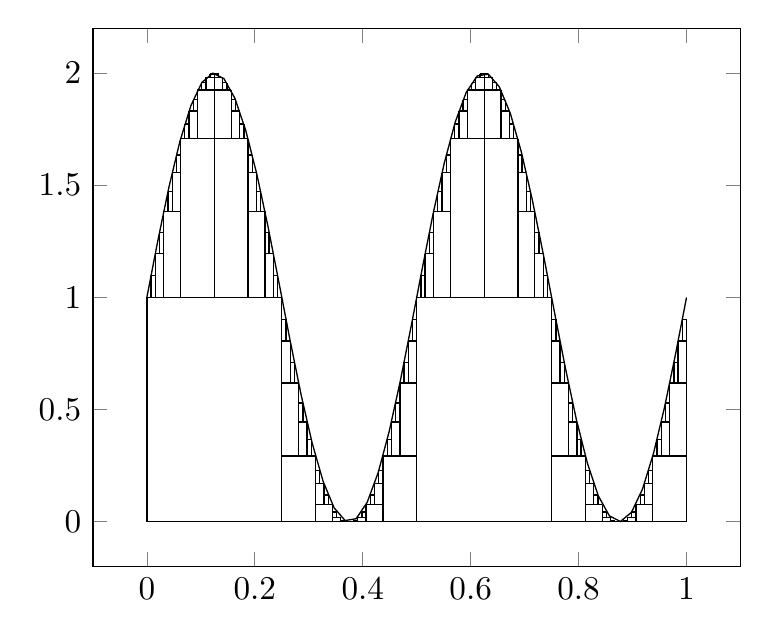
\begin{tikzpicture}[scale=1.2]
\begin{axis}
\addplot[domain=0:1,samples=50] {sin(4*pi*deg(x))+1};
\draw (axis cs: 0, 0) -- (axis cs: 1, 0);
\draw (axis cs: 1, 0) -- (axis cs: 1, 0.0);
\draw (axis cs: 0, 0.0) -- (axis cs: 1, 0.0);
\draw (axis cs: 0, 0.0) -- (axis cs: 0, 0.0);
\draw (axis cs: 1/2, 0.0) -- (axis cs: 1/2, 0.0);
\draw (axis cs: 0, 0.0) -- (axis cs: 1/2, 0.0);
\draw (axis cs: 1/2, 0.0) -- (axis cs: 1/2, 0.0);
\draw (axis cs: 1, 0.0) -- (axis cs: 1, 0.0);
\draw (axis cs: 1/2, 0.0) -- (axis cs: 1, 0.0);
\draw (axis cs: 0, 0.0) -- (axis cs: 0, 1.000000000236429);
\draw (axis cs: 1/4, 0.0) -- (axis cs: 1/4, 1.000000000236429);
\draw (axis cs: 0, 1.000000000236429) -- (axis cs: 1/4, 1.000000000236429);
\draw (axis cs: 1/4, 0.0) -- (axis cs: 1/4, 0.0);
\draw (axis cs: 1/2, 0.0) -- (axis cs: 1/2, 0.0);
\draw (axis cs: 1/4, 0.0) -- (axis cs: 1/2, 0.0);
\draw (axis cs: 1/2, 0.0) -- (axis cs: 1/2, 1.000000011107131);
\draw (axis cs: 3/4, 0.0) -- (axis cs: 3/4, 1.000000011107131);
\draw (axis cs: 1/2, 1.000000011107131) -- (axis cs: 3/4, 1.000000011107131);
\draw (axis cs: 3/4, 0.0) -- (axis cs: 3/4, 0.0);
\draw (axis cs: 1, 0.0) -- (axis cs: 1, 0.0);
\draw (axis cs: 3/4, 0.0) -- (axis cs: 1, 0.0);
\draw (axis cs: 0, 1.000000000236429) -- (axis cs: 0, 1.0000000001838258);
\draw (axis cs: 1/8, 1.000000000236429) -- (axis cs: 1/8, 1.0000000001838258);
\draw (axis cs: 0, 1.0000000001838258) -- (axis cs: 1/8, 1.0000000001838258);
\draw (axis cs: 1/8, 1.000000000236429) -- (axis cs: 1/8, 1.0000000055535658);
\draw (axis cs: 1/4, 1.000000000236429) -- (axis cs: 1/4, 1.0000000055535658);
\draw (axis cs: 1/8, 1.0000000055535658) -- (axis cs: 1/4, 1.0000000055535658);
\draw (axis cs: 1/4, 0.0) -- (axis cs: 1/4, 0.0);
\draw (axis cs: 3/8, 0.0) -- (axis cs: 3/8, 0.0);
\draw (axis cs: 1/4, 0.0) -- (axis cs: 3/8, 0.0);
\draw (axis cs: 3/8, 0.0) -- (axis cs: 3/8, 0.0);
\draw (axis cs: 1/2, 0.0) -- (axis cs: 1/2, 0.0);
\draw (axis cs: 3/8, 0.0) -- (axis cs: 1/2, 0.0);
\draw (axis cs: 1/2, 1.000000011107131) -- (axis cs: 1/2, 1.0000000081305724);
\draw (axis cs: 5/8, 1.000000011107131) -- (axis cs: 5/8, 1.0000000081305724);
\draw (axis cs: 1/2, 1.0000000081305724) -- (axis cs: 5/8, 1.0000000081305724);
\draw (axis cs: 5/8, 1.000000011107131) -- (axis cs: 5/8, 1.0000000139748395);
\draw (axis cs: 3/4, 1.000000011107131) -- (axis cs: 3/4, 1.0000000139748395);
\draw (axis cs: 5/8, 1.0000000139748395) -- (axis cs: 3/4, 1.0000000139748395);
\draw (axis cs: 3/4, 0.0) -- (axis cs: 3/4, 1.1102230246251565E-16);
\draw (axis cs: 7/8, 0.0) -- (axis cs: 7/8, 1.1102230246251565E-16);
\draw (axis cs: 3/4, 1.1102230246251565E-16) -- (axis cs: 7/8, 1.1102230246251565E-16);
\draw (axis cs: 7/8, 0.0) -- (axis cs: 7/8, 1.1102230246251565E-16);
\draw (axis cs: 1, 0.0) -- (axis cs: 1, 1.1102230246251565E-16);
\draw (axis cs: 7/8, 1.1102230246251565E-16) -- (axis cs: 1, 1.1102230246251565E-16);
\draw (axis cs: 0, 1.0000000001838258) -- (axis cs: 0, 1.0000000002503824);
\draw (axis cs: 1/16, 1.0000000001838258) -- (axis cs: 1/16, 1.0000000002503824);
\draw (axis cs: 0, 1.0000000002503824) -- (axis cs: 1/16, 1.0000000002503824);
\draw (axis cs: 1/16, 1.0000000001838258) -- (axis cs: 1/16, 1.707106782400046);
\draw (axis cs: 1/8, 1.0000000001838258) -- (axis cs: 1/8, 1.707106782400046);
\draw (axis cs: 1/16, 1.707106782400046) -- (axis cs: 1/8, 1.707106782400046);
\draw (axis cs: 1/8, 1.0000000055535658) -- (axis cs: 1/8, 1.7071067843635284);
\draw (axis cs: 3/16, 1.0000000055535658) -- (axis cs: 3/16, 1.7071067843635284);
\draw (axis cs: 1/8, 1.7071067843635284) -- (axis cs: 3/16, 1.7071067843635284);
\draw (axis cs: 3/16, 1.0000000055535658) -- (axis cs: 3/16, 1.000000004002456);
\draw (axis cs: 1/4, 1.0000000055535658) -- (axis cs: 1/4, 1.000000004002456);
\draw (axis cs: 3/16, 1.000000004002456) -- (axis cs: 1/4, 1.000000004002456);
\draw (axis cs: 1/4, 0.0) -- (axis cs: 1/4, 0.2928932239539149);
\draw (axis cs: 5/16, 0.0) -- (axis cs: 5/16, 0.2928932239539149);
\draw (axis cs: 1/4, 0.2928932239539149) -- (axis cs: 5/16, 0.2928932239539149);
\draw (axis cs: 5/16, 0.0) -- (axis cs: 5/16, 0.0);
\draw (axis cs: 3/8, 0.0) -- (axis cs: 3/8, 0.0);
\draw (axis cs: 5/16, 0.0) -- (axis cs: 3/8, 0.0);
\draw (axis cs: 3/8, 0.0) -- (axis cs: 3/8, 0.0);
\draw (axis cs: 7/16, 0.0) -- (axis cs: 7/16, 0.0);
\draw (axis cs: 3/8, 0.0) -- (axis cs: 7/16, 0.0);
\draw (axis cs: 7/16, 0.0) -- (axis cs: 7/16, 0.29289322315451494);
\draw (axis cs: 1/2, 0.0) -- (axis cs: 1/2, 0.29289322315451494);
\draw (axis cs: 7/16, 0.29289322315451494) -- (axis cs: 1/2, 0.29289322315451494);
\draw (axis cs: 1/2, 1.0000000081305724) -- (axis cs: 1/2, 1.0000000117626413);
\draw (axis cs: 9/16, 1.0000000081305724) -- (axis cs: 9/16, 1.0000000117626413);
\draw (axis cs: 1/2, 1.0000000117626413) -- (axis cs: 9/16, 1.0000000117626413);
\draw (axis cs: 9/16, 1.0000000081305724) -- (axis cs: 9/16, 1.7071067895039909);
\draw (axis cs: 5/8, 1.0000000081305724) -- (axis cs: 5/8, 1.7071067895039909);
\draw (axis cs: 9/16, 1.7071067895039909) -- (axis cs: 5/8, 1.7071067895039909);
\draw (axis cs: 5/8, 1.0000000139748395) -- (axis cs: 5/8, 1.707106788446632);
\draw (axis cs: 11/16, 1.0000000139748395) -- (axis cs: 11/16, 1.707106788446632);
\draw (axis cs: 5/8, 1.707106788446632) -- (axis cs: 11/16, 1.707106788446632);
\draw (axis cs: 11/16, 1.0000000139748395) -- (axis cs: 11/16, 1.000000019032353);
\draw (axis cs: 3/4, 1.0000000139748395) -- (axis cs: 3/4, 1.000000019032353);
\draw (axis cs: 11/16, 1.000000019032353) -- (axis cs: 3/4, 1.000000019032353);
\draw (axis cs: 3/4, 1.1102230246251565E-16) -- (axis cs: 3/4, 0.2928932322713579);
\draw (axis cs: 13/16, 1.1102230246251565E-16) -- (axis cs: 13/16, 0.2928932322713579);
\draw (axis cs: 3/4, 0.2928932322713579) -- (axis cs: 13/16, 0.2928932322713579);
\draw (axis cs: 13/16, 1.1102230246251565E-16) -- (axis cs: 13/16, 2.220446049250313E-16);
\draw (axis cs: 7/8, 1.1102230246251565E-16) -- (axis cs: 7/8, 2.220446049250313E-16);
\draw (axis cs: 13/16, 2.220446049250313E-16) -- (axis cs: 7/8, 2.220446049250313E-16);
\draw (axis cs: 7/8, 1.1102230246251565E-16) -- (axis cs: 7/8, 2.220446049250313E-16);
\draw (axis cs: 15/16, 1.1102230246251565E-16) -- (axis cs: 15/16, 2.220446049250313E-16);
\draw (axis cs: 7/8, 2.220446049250313E-16) -- (axis cs: 15/16, 2.220446049250313E-16);
\draw (axis cs: 15/16, 1.1102230246251565E-16) -- (axis cs: 15/16, 0.29289323216953733);
\draw (axis cs: 1, 1.1102230246251565E-16) -- (axis cs: 1, 0.29289323216953733);
\draw (axis cs: 15/16, 0.29289323216953733) -- (axis cs: 1, 0.29289323216953733);
\draw (axis cs: 0, 1.0000000002503824) -- (axis cs: 0, 1.000000000202091);
\draw (axis cs: 1/32, 1.0000000002503824) -- (axis cs: 1/32, 1.000000000202091);
\draw (axis cs: 0, 1.000000000202091) -- (axis cs: 1/32, 1.000000000202091);
\draw (axis cs: 1/32, 1.0000000002503824) -- (axis cs: 1/32, 1.382683433157846);
\draw (axis cs: 1/16, 1.0000000002503824) -- (axis cs: 1/16, 1.382683433157846);
\draw (axis cs: 1/32, 1.382683433157846) -- (axis cs: 1/16, 1.382683433157846);
\draw (axis cs: 1/16, 1.707106782400046) -- (axis cs: 1/16, 1.7071067821308197);
\draw (axis cs: 3/32, 1.707106782400046) -- (axis cs: 3/32, 1.7071067821308197);
\draw (axis cs: 1/16, 1.7071067821308197) -- (axis cs: 3/32, 1.7071067821308197);
\draw (axis cs: 3/32, 1.707106782400046) -- (axis cs: 3/32, 1.9238795333709715);
\draw (axis cs: 1/8, 1.707106782400046) -- (axis cs: 1/8, 1.9238795333709715);
\draw (axis cs: 3/32, 1.9238795333709715) -- (axis cs: 1/8, 1.9238795333709715);
\draw (axis cs: 1/8, 1.7071067843635284) -- (axis cs: 1/8, 1.9238795339022858);
\draw (axis cs: 5/32, 1.7071067843635284) -- (axis cs: 5/32, 1.9238795339022858);
\draw (axis cs: 1/8, 1.9238795339022858) -- (axis cs: 5/32, 1.9238795339022858);
\draw (axis cs: 5/32, 1.7071067843635284) -- (axis cs: 5/32, 1.7071067835903304);
\draw (axis cs: 3/16, 1.7071067843635284) -- (axis cs: 3/16, 1.7071067835903304);
\draw (axis cs: 5/32, 1.7071067835903304) -- (axis cs: 3/16, 1.7071067835903304);
\draw (axis cs: 3/16, 1.000000004002456) -- (axis cs: 3/16, 1.3826834351429769);
\draw (axis cs: 7/32, 1.000000004002456) -- (axis cs: 7/32, 1.3826834351429769);
\draw (axis cs: 3/16, 1.3826834351429769) -- (axis cs: 7/32, 1.3826834351429769);
\draw (axis cs: 7/32, 1.000000004002456) -- (axis cs: 7/32, 1.0000000058813205);
\draw (axis cs: 1/4, 1.000000004002456) -- (axis cs: 1/4, 1.0000000058813205);
\draw (axis cs: 7/32, 1.0000000058813205) -- (axis cs: 1/4, 1.0000000058813205);
\draw (axis cs: 1/4, 0.2928932239539149) -- (axis cs: 1/4, 0.6173165730453525);
\draw (axis cs: 9/32, 0.2928932239539149) -- (axis cs: 9/32, 0.6173165730453525);
\draw (axis cs: 1/4, 0.6173165730453525) -- (axis cs: 9/32, 0.6173165730453525);
\draw (axis cs: 9/32, 0.2928932239539149) -- (axis cs: 9/32, 0.29289322267674545);
\draw (axis cs: 5/16, 0.2928932239539149) -- (axis cs: 5/16, 0.29289322267674545);
\draw (axis cs: 9/32, 0.29289322267674545) -- (axis cs: 5/16, 0.29289322267674545);
\draw (axis cs: 5/16, 0.0) -- (axis cs: 5/16, 0.07612046942923334);
\draw (axis cs: 11/32, 0.0) -- (axis cs: 11/32, 0.07612046942923334);
\draw (axis cs: 5/16, 0.07612046942923334) -- (axis cs: 11/32, 0.07612046942923334);
\draw (axis cs: 11/32, 0.0) -- (axis cs: 11/32, 0.0);
\draw (axis cs: 3/8, 0.0) -- (axis cs: 3/8, 0.0);
\draw (axis cs: 11/32, 0.0) -- (axis cs: 3/8, 0.0);
\draw (axis cs: 3/8, 0.0) -- (axis cs: 3/8, 0.0);
\draw (axis cs: 13/32, 0.0) -- (axis cs: 13/32, 0.0);
\draw (axis cs: 3/8, 0.0) -- (axis cs: 13/32, 0.0);
\draw (axis cs: 13/32, 0.0) -- (axis cs: 13/32, 0.076120471130396);
\draw (axis cs: 7/16, 0.0) -- (axis cs: 7/16, 0.076120471130396);
\draw (axis cs: 13/32, 0.076120471130396) -- (axis cs: 7/16, 0.076120471130396);
\draw (axis cs: 7/16, 0.29289322315451494) -- (axis cs: 7/16, 0.29289322554240516);
\draw (axis cs: 15/32, 0.29289322315451494) -- (axis cs: 15/32, 0.29289322554240516);
\draw (axis cs: 7/16, 0.29289322554240516) -- (axis cs: 15/32, 0.29289322554240516);
\draw (axis cs: 15/32, 0.29289322315451494) -- (axis cs: 15/32, 0.6173165763021443);
\draw (axis cs: 1/2, 0.29289322315451494) -- (axis cs: 1/2, 0.6173165763021443);
\draw (axis cs: 15/32, 0.6173165763021443) -- (axis cs: 1/2, 0.6173165763021443);
\draw (axis cs: 1/2, 1.0000000117626413) -- (axis cs: 1/2, 1.000000008988646);
\draw (axis cs: 17/32, 1.0000000117626413) -- (axis cs: 17/32, 1.000000008988646);
\draw (axis cs: 1/2, 1.000000008988646) -- (axis cs: 17/32, 1.000000008988646);
\draw (axis cs: 17/32, 1.0000000117626413) -- (axis cs: 17/32, 1.3826834403067085);
\draw (axis cs: 9/16, 1.0000000117626413) -- (axis cs: 9/16, 1.3826834403067085);
\draw (axis cs: 17/32, 1.3826834403067085) -- (axis cs: 9/16, 1.3826834403067085);
\draw (axis cs: 9/16, 1.7071067895039909) -- (axis cs: 9/16, 1.7071067869871195);
\draw (axis cs: 19/32, 1.7071067895039909) -- (axis cs: 19/32, 1.7071067869871195);
\draw (axis cs: 9/16, 1.7071067869871195) -- (axis cs: 19/32, 1.7071067869871195);
\draw (axis cs: 19/32, 1.7071067895039909) -- (axis cs: 19/32, 1.923879535500254);
\draw (axis cs: 5/8, 1.7071067895039909) -- (axis cs: 5/8, 1.923879535500254);
\draw (axis cs: 19/32, 1.923879535500254) -- (axis cs: 5/8, 1.923879535500254);
\draw (axis cs: 5/8, 1.707106788446632) -- (axis cs: 5/8, 1.9238795384036536);
\draw (axis cs: 21/32, 1.707106788446632) -- (axis cs: 21/32, 1.9238795384036536);
\draw (axis cs: 5/8, 1.9238795384036536) -- (axis cs: 21/32, 1.9238795384036536);
\draw (axis cs: 21/32, 1.707106788446632) -- (axis cs: 21/32, 1.7071067920742213);
\draw (axis cs: 11/16, 1.707106788446632) -- (axis cs: 11/16, 1.7071067920742213);
\draw (axis cs: 21/32, 1.7071067920742213) -- (axis cs: 11/16, 1.7071067920742213);
\draw (axis cs: 11/16, 1.000000019032353) -- (axis cs: 11/16, 1.3826834465905207);
\draw (axis cs: 23/32, 1.000000019032353) -- (axis cs: 23/32, 1.3826834465905207);
\draw (axis cs: 11/16, 1.3826834465905207) -- (axis cs: 23/32, 1.3826834465905207);
\draw (axis cs: 23/32, 1.000000019032353) -- (axis cs: 23/32, 1.0000000153632311);
\draw (axis cs: 3/4, 1.000000019032353) -- (axis cs: 3/4, 1.0000000153632311);
\draw (axis cs: 23/32, 1.0000000153632311) -- (axis cs: 3/4, 1.0000000153632311);
\draw (axis cs: 3/4, 0.2928932322713579) -- (axis cs: 3/4, 0.6173165814658779);
\draw (axis cs: 25/32, 0.2928932322713579) -- (axis cs: 25/32, 0.6173165814658779);
\draw (axis cs: 3/4, 0.6173165814658779) -- (axis cs: 25/32, 0.6173165814658779);
\draw (axis cs: 25/32, 0.2928932322713579) -- (axis cs: 25/32, 0.2928932291215375);
\draw (axis cs: 13/16, 0.2928932322713579) -- (axis cs: 13/16, 0.2928932291215375);
\draw (axis cs: 25/32, 0.2928932291215375) -- (axis cs: 13/16, 0.2928932291215375);
\draw (axis cs: 13/16, 2.220446049250313E-16) -- (axis cs: 13/16, 0.07612047291712909);
\draw (axis cs: 27/32, 2.220446049250313E-16) -- (axis cs: 27/32, 0.07612047291712909);
\draw (axis cs: 13/16, 0.07612047291712909) -- (axis cs: 27/32, 0.07612047291712909);
\draw (axis cs: 27/32, 2.220446049250313E-16) -- (axis cs: 27/32, 1.1102230246251565E-16);
\draw (axis cs: 7/8, 2.220446049250313E-16) -- (axis cs: 7/8, 1.1102230246251565E-16);
\draw (axis cs: 27/32, 1.1102230246251565E-16) -- (axis cs: 7/8, 1.1102230246251565E-16);
\draw (axis cs: 7/8, 2.220446049250313E-16) -- (axis cs: 7/8, 1.1102230246251565E-16);
\draw (axis cs: 29/32, 2.220446049250313E-16) -- (axis cs: 29/32, 1.1102230246251565E-16);
\draw (axis cs: 7/8, 1.1102230246251565E-16) -- (axis cs: 29/32, 1.1102230246251565E-16);
\draw (axis cs: 29/32, 2.220446049250313E-16) -- (axis cs: 29/32, 0.07612047261656973);
\draw (axis cs: 15/16, 2.220446049250313E-16) -- (axis cs: 15/16, 0.07612047261656973);
\draw (axis cs: 29/32, 0.07612047261656973) -- (axis cs: 15/16, 0.07612047261656973);
\draw (axis cs: 15/16, 0.29289323216953733) -- (axis cs: 15/16, 0.29289322801081585);
\draw (axis cs: 31/32, 0.29289323216953733) -- (axis cs: 31/32, 0.29289322801081585);
\draw (axis cs: 15/16, 0.29289322801081585) -- (axis cs: 31/32, 0.29289322801081585);
\draw (axis cs: 31/32, 0.29289323216953733) -- (axis cs: 31/32, 0.617316579289038);
\draw (axis cs: 1, 0.29289323216953733) -- (axis cs: 1, 0.617316579289038);
\draw (axis cs: 31/32, 0.617316579289038) -- (axis cs: 1, 0.617316579289038);
\draw (axis cs: 0, 1.000000000202091) -- (axis cs: 0, 1.0000000001394955);
\draw (axis cs: 1/64, 1.000000000202091) -- (axis cs: 1/64, 1.0000000001394955);
\draw (axis cs: 0, 1.0000000001394955) -- (axis cs: 1/64, 1.0000000001394955);
\draw (axis cs: 1/64, 1.000000000202091) -- (axis cs: 1/64, 1.1950903223811593);
\draw (axis cs: 1/32, 1.000000000202091) -- (axis cs: 1/32, 1.1950903223811593);
\draw (axis cs: 1/64, 1.1950903223811593) -- (axis cs: 1/32, 1.1950903223811593);
\draw (axis cs: 1/32, 1.382683433157846) -- (axis cs: 1/32, 1.3826834329239164);
\draw (axis cs: 3/64, 1.382683433157846) -- (axis cs: 3/64, 1.3826834329239164);
\draw (axis cs: 1/32, 1.3826834329239164) -- (axis cs: 3/64, 1.3826834329239164);
\draw (axis cs: 3/64, 1.382683433157846) -- (axis cs: 3/64, 1.5555702339364768);
\draw (axis cs: 1/16, 1.382683433157846) -- (axis cs: 1/16, 1.5555702339364768);
\draw (axis cs: 3/64, 1.5555702339364768) -- (axis cs: 1/16, 1.5555702339364768);
\draw (axis cs: 1/16, 1.7071067821308197) -- (axis cs: 1/16, 1.707106782471663);
\draw (axis cs: 5/64, 1.7071067821308197) -- (axis cs: 5/64, 1.707106782471663);
\draw (axis cs: 1/16, 1.707106782471663) -- (axis cs: 5/64, 1.707106782471663);
\draw (axis cs: 5/64, 1.7071067821308197) -- (axis cs: 5/64, 1.831469613312254);
\draw (axis cs: 3/32, 1.7071067821308197) -- (axis cs: 3/32, 1.831469613312254);
\draw (axis cs: 5/64, 1.831469613312254) -- (axis cs: 3/32, 1.831469613312254);
\draw (axis cs: 3/32, 1.9238795333709715) -- (axis cs: 3/32, 1.923879533137701);
\draw (axis cs: 7/64, 1.9238795333709715) -- (axis cs: 7/64, 1.923879533137701);
\draw (axis cs: 3/32, 1.923879533137701) -- (axis cs: 7/64, 1.923879533137701);
\draw (axis cs: 7/64, 1.9238795333709715) -- (axis cs: 7/64, 1.9807852809769249);
\draw (axis cs: 1/8, 1.9238795333709715) -- (axis cs: 1/8, 1.9807852809769249);
\draw (axis cs: 7/64, 1.9807852809769249) -- (axis cs: 1/8, 1.9807852809769249);
\draw (axis cs: 1/8, 1.9238795339022858) -- (axis cs: 1/8, 1.9807852809622184);
\draw (axis cs: 9/64, 1.9238795339022858) -- (axis cs: 9/64, 1.9807852809622184);
\draw (axis cs: 1/8, 1.9807852809622184) -- (axis cs: 9/64, 1.9807852809622184);
\draw (axis cs: 9/64, 1.9238795339022858) -- (axis cs: 9/64, 1.9238795335326417);
\draw (axis cs: 5/32, 1.9238795339022858) -- (axis cs: 5/32, 1.9238795335326417);
\draw (axis cs: 9/64, 1.9238795335326417) -- (axis cs: 5/32, 1.9238795335326417);
\draw (axis cs: 5/32, 1.7071067835903304) -- (axis cs: 5/32, 1.831469613676237);
\draw (axis cs: 11/64, 1.7071067835903304) -- (axis cs: 11/64, 1.831469613676237);
\draw (axis cs: 5/32, 1.831469613676237) -- (axis cs: 11/64, 1.831469613676237);
\draw (axis cs: 11/64, 1.7071067835903304) -- (axis cs: 11/64, 1.707106784551024);
\draw (axis cs: 3/16, 1.7071067835903304) -- (axis cs: 3/16, 1.707106784551024);
\draw (axis cs: 11/64, 1.707106784551024) -- (axis cs: 3/16, 1.707106784551024);
\draw (axis cs: 3/16, 1.3826834351429769) -- (axis cs: 3/16, 1.5555702369758078);
\draw (axis cs: 13/64, 1.3826834351429769) -- (axis cs: 13/64, 1.5555702369758078);
\draw (axis cs: 3/16, 1.5555702369758078) -- (axis cs: 13/64, 1.5555702369758078);
\draw (axis cs: 13/64, 1.3826834351429769) -- (axis cs: 13/64, 1.3826834367609901);
\draw (axis cs: 7/32, 1.3826834351429769) -- (axis cs: 7/32, 1.3826834367609901);
\draw (axis cs: 13/64, 1.3826834367609901) -- (axis cs: 7/32, 1.3826834367609901);
\draw (axis cs: 7/32, 1.0000000058813205) -- (axis cs: 7/32, 1.1950903265550472);
\draw (axis cs: 15/64, 1.0000000058813205) -- (axis cs: 15/64, 1.1950903265550472);
\draw (axis cs: 7/32, 1.1950903265550472) -- (axis cs: 15/64, 1.1950903265550472);
\draw (axis cs: 15/64, 1.0000000058813205) -- (axis cs: 15/64, 1.0000000044314918);
\draw (axis cs: 1/4, 1.0000000058813205) -- (axis cs: 1/4, 1.0000000044314918);
\draw (axis cs: 15/64, 1.0000000044314918) -- (axis cs: 1/4, 1.0000000044314918);
\draw (axis cs: 1/4, 0.6173165730453525) -- (axis cs: 1/4, 0.8049096821376361);
\draw (axis cs: 17/64, 0.6173165730453525) -- (axis cs: 17/64, 0.8049096821376361);
\draw (axis cs: 1/4, 0.8049096821376361) -- (axis cs: 17/64, 0.8049096821376361);
\draw (axis cs: 17/64, 0.6173165730453525) -- (axis cs: 17/64, 0.6173165713662676);
\draw (axis cs: 9/32, 0.6173165730453525) -- (axis cs: 9/32, 0.6173165713662676);
\draw (axis cs: 17/64, 0.6173165713662676) -- (axis cs: 9/32, 0.6173165713662676);
\draw (axis cs: 9/32, 0.29289322267674545) -- (axis cs: 9/32, 0.44442977338167267);
\draw (axis cs: 19/64, 0.29289322267674545) -- (axis cs: 19/64, 0.44442977338167267);
\draw (axis cs: 9/32, 0.44442977338167267) -- (axis cs: 19/64, 0.44442977338167267);
\draw (axis cs: 19/64, 0.29289322267674545) -- (axis cs: 19/64, 0.2928932242572895);
\draw (axis cs: 5/16, 0.29289322267674545) -- (axis cs: 5/16, 0.2928932242572895);
\draw (axis cs: 19/64, 0.2928932242572895) -- (axis cs: 5/16, 0.2928932242572895);
\draw (axis cs: 5/16, 0.07612046942923334) -- (axis cs: 5/16, 0.16853039197465014);
\draw (axis cs: 21/64, 0.07612046942923334) -- (axis cs: 21/64, 0.16853039197465014);
\draw (axis cs: 5/16, 0.16853039197465014) -- (axis cs: 21/64, 0.16853039197465014);
\draw (axis cs: 21/64, 0.07612046942923334) -- (axis cs: 21/64, 0.07612047043489656);
\draw (axis cs: 11/32, 0.07612046942923334) -- (axis cs: 11/32, 0.07612047043489656);
\draw (axis cs: 21/64, 0.07612047043489656) -- (axis cs: 11/32, 0.07612047043489656);
\draw (axis cs: 11/32, 0.0) -- (axis cs: 11/32, 0.0192147210987208);
\draw (axis cs: 23/64, 0.0) -- (axis cs: 23/64, 0.0192147210987208);
\draw (axis cs: 11/32, 0.0192147210987208) -- (axis cs: 23/64, 0.0192147210987208);
\draw (axis cs: 23/64, 0.0) -- (axis cs: 23/64, 0.0);
\draw (axis cs: 3/8, 0.0) -- (axis cs: 3/8, 0.0);
\draw (axis cs: 23/64, 0.0) -- (axis cs: 3/8, 0.0);
\draw (axis cs: 3/8, 0.0) -- (axis cs: 3/8, 0.0);
\draw (axis cs: 25/64, 0.0) -- (axis cs: 25/64, 0.0);
\draw (axis cs: 3/8, 0.0) -- (axis cs: 25/64, 0.0);
\draw (axis cs: 25/64, 0.0) -- (axis cs: 25/64, 0.019214721044814476);
\draw (axis cs: 13/32, 0.0) -- (axis cs: 13/32, 0.019214721044814476);
\draw (axis cs: 25/64, 0.019214721044814476) -- (axis cs: 13/32, 0.019214721044814476);
\draw (axis cs: 13/32, 0.076120471130396) -- (axis cs: 13/32, 0.07612047025401592);
\draw (axis cs: 27/64, 0.076120471130396) -- (axis cs: 27/64, 0.07612047025401592);
\draw (axis cs: 13/32, 0.07612047025401592) -- (axis cs: 27/64, 0.07612047025401592);
\draw (axis cs: 27/64, 0.076120471130396) -- (axis cs: 27/64, 0.168530391602966);
\draw (axis cs: 7/16, 0.076120471130396) -- (axis cs: 7/16, 0.168530391602966);
\draw (axis cs: 27/64, 0.168530391602966) -- (axis cs: 7/16, 0.168530391602966);
\draw (axis cs: 7/16, 0.29289322554240516) -- (axis cs: 7/16, 0.2928932236453855);
\draw (axis cs: 29/64, 0.29289322554240516) -- (axis cs: 29/64, 0.2928932236453855);
\draw (axis cs: 7/16, 0.2928932236453855) -- (axis cs: 29/64, 0.2928932236453855);
\draw (axis cs: 29/64, 0.29289322554240516) -- (axis cs: 29/64, 0.4444297724988914);
\draw (axis cs: 15/32, 0.29289322554240516) -- (axis cs: 15/32, 0.4444297724988914);
\draw (axis cs: 29/64, 0.4444297724988914) -- (axis cs: 15/32, 0.4444297724988914);
\draw (axis cs: 15/32, 0.6173165763021443) -- (axis cs: 15/32, 0.6173165735853278);
\draw (axis cs: 31/64, 0.6173165763021443) -- (axis cs: 31/64, 0.6173165735853278);
\draw (axis cs: 15/32, 0.6173165735853278) -- (axis cs: 31/64, 0.6173165735853278);
\draw (axis cs: 31/64, 0.6173165763021443) -- (axis cs: 31/64, 0.8049096841082247);
\draw (axis cs: 1/2, 0.6173165763021443) -- (axis cs: 1/2, 0.8049096841082247);
\draw (axis cs: 31/64, 0.8049096841082247) -- (axis cs: 1/2, 0.8049096841082247);
\draw (axis cs: 1/2, 1.000000008988646) -- (axis cs: 1/2, 1.0000000124568353);
\draw (axis cs: 33/64, 1.000000008988646) -- (axis cs: 33/64, 1.0000000124568353);
\draw (axis cs: 1/2, 1.0000000124568353) -- (axis cs: 33/64, 1.0000000124568353);
\draw (axis cs: 33/64, 1.000000008988646) -- (axis cs: 33/64, 1.1950903342336092);
\draw (axis cs: 17/32, 1.000000008988646) -- (axis cs: 17/32, 1.1950903342336092);
\draw (axis cs: 33/64, 1.1950903342336092) -- (axis cs: 17/32, 1.1950903342336092);
\draw (axis cs: 17/32, 1.3826834403067085) -- (axis cs: 17/32, 1.3826834438737055);
\draw (axis cs: 35/64, 1.3826834403067085) -- (axis cs: 35/64, 1.3826834438737055);
\draw (axis cs: 17/32, 1.3826834438737055) -- (axis cs: 35/64, 1.3826834438737055);
\draw (axis cs: 35/64, 1.3826834403067085) -- (axis cs: 35/64, 1.5555702433770828);
\draw (axis cs: 9/16, 1.3826834403067085) -- (axis cs: 9/16, 1.5555702433770828);
\draw (axis cs: 35/64, 1.5555702433770828) -- (axis cs: 9/16, 1.5555702433770828);
\draw (axis cs: 9/16, 1.7071067869871195) -- (axis cs: 9/16, 1.7071067899948602);
\draw (axis cs: 37/64, 1.7071067869871195) -- (axis cs: 37/64, 1.7071067899948602);
\draw (axis cs: 9/16, 1.7071067899948602) -- (axis cs: 37/64, 1.7071067899948602);
\draw (axis cs: 37/64, 1.7071067869871195) -- (axis cs: 37/64, 1.831469619223192);
\draw (axis cs: 19/32, 1.7071067869871195) -- (axis cs: 19/32, 1.831469619223192);
\draw (axis cs: 37/64, 1.831469619223192) -- (axis cs: 19/32, 1.831469619223192);
\draw (axis cs: 19/32, 1.923879535500254) -- (axis cs: 19/32, 1.9238795372783113);
\draw (axis cs: 39/64, 1.923879535500254) -- (axis cs: 39/64, 1.9238795372783113);
\draw (axis cs: 19/32, 1.9238795372783113) -- (axis cs: 39/64, 1.9238795372783113);
\draw (axis cs: 39/64, 1.923879535500254) -- (axis cs: 39/64, 1.980785282816944);
\draw (axis cs: 5/8, 1.923879535500254) -- (axis cs: 5/8, 1.980785282816944);
\draw (axis cs: 39/64, 1.980785282816944) -- (axis cs: 5/8, 1.980785282816944);
\draw (axis cs: 5/8, 1.9238795384036536) -- (axis cs: 5/8, 1.9807852827403325);
\draw (axis cs: 41/64, 1.9238795384036536) -- (axis cs: 41/64, 1.9807852827403325);
\draw (axis cs: 5/8, 1.9807852827403325) -- (axis cs: 41/64, 1.9807852827403325);
\draw (axis cs: 41/64, 1.9238795384036536) -- (axis cs: 41/64, 1.9238795370205377);
\draw (axis cs: 21/32, 1.9238795384036536) -- (axis cs: 21/32, 1.9238795370205377);
\draw (axis cs: 41/64, 1.9238795370205377) -- (axis cs: 21/32, 1.9238795370205377);
\draw (axis cs: 21/32, 1.7071067920742213) -- (axis cs: 21/32, 1.8314696187398765);
\draw (axis cs: 43/64, 1.7071067920742213) -- (axis cs: 43/64, 1.8314696187398765);
\draw (axis cs: 21/32, 1.8314696187398765) -- (axis cs: 43/64, 1.8314696187398765);
\draw (axis cs: 43/64, 1.7071067920742213) -- (axis cs: 43/64, 1.7071067892408764);
\draw (axis cs: 11/16, 1.7071067920742213) -- (axis cs: 11/16, 1.7071067892408764);
\draw (axis cs: 43/64, 1.7071067892408764) -- (axis cs: 11/16, 1.7071067892408764);
\draw (axis cs: 11/16, 1.3826834465905207) -- (axis cs: 11/16, 1.5555702423272328);
\draw (axis cs: 45/64, 1.3826834465905207) -- (axis cs: 45/64, 1.5555702423272328);
\draw (axis cs: 11/16, 1.5555702423272328) -- (axis cs: 45/64, 1.5555702423272328);
\draw (axis cs: 45/64, 1.3826834465905207) -- (axis cs: 45/64, 1.3826834425257721);
\draw (axis cs: 23/32, 1.3826834465905207) -- (axis cs: 23/32, 1.3826834425257721);
\draw (axis cs: 45/64, 1.3826834425257721) -- (axis cs: 23/32, 1.3826834425257721);
\draw (axis cs: 23/32, 1.0000000153632311) -- (axis cs: 23/32, 1.1950903326100732);
\draw (axis cs: 47/64, 1.0000000153632311) -- (axis cs: 47/64, 1.1950903326100732);
\draw (axis cs: 23/32, 1.1950903326100732) -- (axis cs: 47/64, 1.1950903326100732);
\draw (axis cs: 47/64, 1.0000000153632311) -- (axis cs: 47/64, 1.0000000106051439);
\draw (axis cs: 3/4, 1.0000000153632311) -- (axis cs: 3/4, 1.0000000106051439);
\draw (axis cs: 47/64, 1.0000000106051439) -- (axis cs: 3/4, 1.0000000106051439);
\draw (axis cs: 3/4, 0.6173165814658779) -- (axis cs: 3/4, 0.8049096881926627);
\draw (axis cs: 49/64, 0.6173165814658779) -- (axis cs: 49/64, 0.8049096881926627);
\draw (axis cs: 3/4, 0.8049096881926627) -- (axis cs: 49/64, 0.8049096881926627);
\draw (axis cs: 49/64, 0.6173165814658779) -- (axis cs: 49/64, 0.6173165770699784);
\draw (axis cs: 25/32, 0.6173165814658779) -- (axis cs: 25/32, 0.6173165770699784);
\draw (axis cs: 49/64, 0.6173165770699784) -- (axis cs: 25/32, 0.6173165770699784);
\draw (axis cs: 25/32, 0.2928932291215375) -- (axis cs: 25/32, 0.44442978373915387);
\draw (axis cs: 51/64, 0.2928932291215375) -- (axis cs: 51/64, 0.44442978373915387);
\draw (axis cs: 25/32, 0.44442978373915387) -- (axis cs: 51/64, 0.44442978373915387);
\draw (axis cs: 51/64, 0.2928932291215375) -- (axis cs: 51/64, 0.29289323306560355);
\draw (axis cs: 13/16, 0.2928932291215375) -- (axis cs: 13/16, 0.29289323306560355);
\draw (axis cs: 51/64, 0.29289323306560355) -- (axis cs: 13/16, 0.29289323306560355);
\draw (axis cs: 13/16, 0.07612047291712909) -- (axis cs: 13/16, 0.16853039889529742);
\draw (axis cs: 53/64, 0.07612047291712909) -- (axis cs: 53/64, 0.16853039889529742);
\draw (axis cs: 13/16, 0.16853039889529742) -- (axis cs: 53/64, 0.16853039889529742);
\draw (axis cs: 53/64, 0.07612047291712909) -- (axis cs: 53/64, 0.07612047520192178);
\draw (axis cs: 27/32, 0.07612047291712909) -- (axis cs: 27/32, 0.07612047520192178);
\draw (axis cs: 53/64, 0.07612047520192178) -- (axis cs: 27/32, 0.07612047520192178);
\draw (axis cs: 27/32, 1.1102230246251565E-16) -- (axis cs: 27/32, 0.01921472352892939);
\draw (axis cs: 55/64, 1.1102230246251565E-16) -- (axis cs: 55/64, 0.01921472352892939);
\draw (axis cs: 27/32, 0.01921472352892939) -- (axis cs: 55/64, 0.01921472352892939);
\draw (axis cs: 55/64, 1.1102230246251565E-16) -- (axis cs: 55/64, 2.220446049250313E-16);
\draw (axis cs: 7/8, 1.1102230246251565E-16) -- (axis cs: 7/8, 2.220446049250313E-16);
\draw (axis cs: 55/64, 2.220446049250313E-16) -- (axis cs: 7/8, 2.220446049250313E-16);
\draw (axis cs: 7/8, 1.1102230246251565E-16) -- (axis cs: 7/8, 2.220446049250313E-16);
\draw (axis cs: 57/64, 1.1102230246251565E-16) -- (axis cs: 57/64, 2.220446049250313E-16);
\draw (axis cs: 7/8, 2.220446049250313E-16) -- (axis cs: 57/64, 2.220446049250313E-16);
\draw (axis cs: 57/64, 1.1102230246251565E-16) -- (axis cs: 57/64, 0.01921472352892928);
\draw (axis cs: 29/32, 1.1102230246251565E-16) -- (axis cs: 29/32, 0.01921472352892928);
\draw (axis cs: 57/64, 0.01921472352892928) -- (axis cs: 29/32, 0.01921472352892928);
\draw (axis cs: 29/32, 0.07612047261656973) -- (axis cs: 29/32, 0.07612047520192144);
\draw (axis cs: 59/64, 0.07612047261656973) -- (axis cs: 59/64, 0.07612047520192144);
\draw (axis cs: 29/32, 0.07612047520192144) -- (axis cs: 59/64, 0.07612047520192144);
\draw (axis cs: 59/64, 0.07612047261656973) -- (axis cs: 59/64, 0.16853039889529697);
\draw (axis cs: 15/16, 0.07612047261656973) -- (axis cs: 15/16, 0.16853039889529697);
\draw (axis cs: 59/64, 0.16853039889529697) -- (axis cs: 15/16, 0.16853039889529697);
\draw (axis cs: 15/16, 0.29289322801081585) -- (axis cs: 15/16, 0.292893233065603);
\draw (axis cs: 61/64, 0.29289322801081585) -- (axis cs: 61/64, 0.292893233065603);
\draw (axis cs: 15/16, 0.292893233065603) -- (axis cs: 61/64, 0.292893233065603);
\draw (axis cs: 61/64, 0.29289322801081585) -- (axis cs: 61/64, 0.4444297837391532);
\draw (axis cs: 31/32, 0.29289322801081585) -- (axis cs: 31/32, 0.4444297837391532);
\draw (axis cs: 61/64, 0.4444297837391532) -- (axis cs: 31/32, 0.4444297837391532);
\draw (axis cs: 31/32, 0.617316579289038) -- (axis cs: 31/32, 0.6173165862562409);
\draw (axis cs: 63/64, 0.617316579289038) -- (axis cs: 63/64, 0.6173165862562409);
\draw (axis cs: 31/32, 0.6173165862562409) -- (axis cs: 63/64, 0.6173165862562409);
\draw (axis cs: 63/64, 0.617316579289038) -- (axis cs: 63/64, 0.8049096977140695);
\draw (axis cs: 1, 0.617316579289038) -- (axis cs: 1, 0.8049096977140695);
\draw (axis cs: 63/64, 0.8049096977140695) -- (axis cs: 1, 0.8049096977140695);
\draw (axis cs: 0, 1.0000000001394955) -- (axis cs: 0, 1.0000000002145182);
\draw (axis cs: 1/128, 1.0000000001394955) -- (axis cs: 1/128, 1.0000000002145182);
\draw (axis cs: 0, 1.0000000002145182) -- (axis cs: 1/128, 1.0000000002145182);
\draw (axis cs: 1/128, 1.0000000001394955) -- (axis cs: 1/128, 1.0980171406657118);
\draw (axis cs: 1/64, 1.0000000001394955) -- (axis cs: 1/64, 1.0980171406657118);
\draw (axis cs: 1/128, 1.0980171406657118) -- (axis cs: 1/64, 1.0980171406657118);
\draw (axis cs: 1/64, 1.1950903223811593) -- (axis cs: 1/64, 1.1950903225669531);
\draw (axis cs: 3/128, 1.1950903223811593) -- (axis cs: 3/128, 1.1950903225669531);
\draw (axis cs: 1/64, 1.1950903225669531) -- (axis cs: 3/128, 1.1950903225669531);
\draw (axis cs: 3/128, 1.1950903223811593) -- (axis cs: 3/128, 1.2902846777219525);
\draw (axis cs: 1/32, 1.1950903223811593) -- (axis cs: 1/32, 1.2902846777219525);
\draw (axis cs: 3/128, 1.2902846777219525) -- (axis cs: 1/32, 1.2902846777219525);
\draw (axis cs: 1/32, 1.3826834329239164) -- (axis cs: 1/32, 1.3826834332046318);
\draw (axis cs: 5/128, 1.3826834329239164) -- (axis cs: 5/128, 1.3826834332046318);
\draw (axis cs: 1/32, 1.3826834332046318) -- (axis cs: 5/128, 1.3826834332046318);
\draw (axis cs: 5/128, 1.3826834329239164) -- (axis cs: 5/128, 1.4713967375789754);
\draw (axis cs: 3/64, 1.3826834329239164) -- (axis cs: 3/64, 1.4713967375789754);
\draw (axis cs: 5/128, 1.4713967375789754) -- (axis cs: 3/64, 1.4713967375789754);
\draw (axis cs: 3/64, 1.5555702339364768) -- (axis cs: 3/64, 1.5555702336478754);
\draw (axis cs: 7/128, 1.5555702339364768) -- (axis cs: 7/128, 1.5555702336478754);
\draw (axis cs: 3/64, 1.5555702336478754) -- (axis cs: 7/128, 1.5555702336478754);
\draw (axis cs: 7/128, 1.5555702339364768) -- (axis cs: 7/128, 1.6343932853002259);
\draw (axis cs: 1/16, 1.5555702339364768) -- (axis cs: 1/16, 1.6343932853002259);
\draw (axis cs: 7/128, 1.6343932853002259) -- (axis cs: 1/16, 1.6343932853002259);
\draw (axis cs: 1/16, 1.707106782471663) -- (axis cs: 1/16, 1.7071067822245676);
\draw (axis cs: 9/128, 1.707106782471663) -- (axis cs: 9/128, 1.7071067822245676);
\draw (axis cs: 1/16, 1.7071067822245676) -- (axis cs: 9/128, 1.7071067822245676);
\draw (axis cs: 9/128, 1.707106782471663) -- (axis cs: 9/128, 1.7730104542317335);
\draw (axis cs: 5/64, 1.707106782471663) -- (axis cs: 5/64, 1.7730104542317335);
\draw (axis cs: 9/128, 1.7730104542317335) -- (axis cs: 5/64, 1.7730104542317335);
\draw (axis cs: 5/64, 1.831469613312254) -- (axis cs: 5/64, 1.8314696130090264);
\draw (axis cs: 11/128, 1.831469613312254) -- (axis cs: 11/128, 1.8314696130090264);
\draw (axis cs: 5/64, 1.8314696130090264) -- (axis cs: 11/128, 1.8314696130090264);
\draw (axis cs: 11/128, 1.831469613312254) -- (axis cs: 11/128, 1.8819212654698285);
\draw (axis cs: 3/32, 1.831469613312254) -- (axis cs: 3/32, 1.8819212654698285);
\draw (axis cs: 11/128, 1.8819212654698285) -- (axis cs: 3/32, 1.8819212654698285);
\draw (axis cs: 3/32, 1.923879533137701) -- (axis cs: 3/32, 1.9238795334217076);
\draw (axis cs: 13/128, 1.923879533137701) -- (axis cs: 13/128, 1.9238795334217076);
\draw (axis cs: 3/32, 1.9238795334217076) -- (axis cs: 13/128, 1.9238795334217076);
\draw (axis cs: 13/128, 1.923879533137701) -- (axis cs: 13/128, 1.9569403364228088);
\draw (axis cs: 7/64, 1.923879533137701) -- (axis cs: 7/64, 1.9569403364228088);
\draw (axis cs: 13/128, 1.9569403364228088) -- (axis cs: 7/64, 1.9569403364228088);
\draw (axis cs: 7/64, 1.9807852809769249) -- (axis cs: 7/64, 1.9807852808615491);
\draw (axis cs: 15/128, 1.9807852809769249) -- (axis cs: 15/128, 1.9807852808615491);
\draw (axis cs: 7/64, 1.9807852808615491) -- (axis cs: 15/128, 1.9807852808615491);
\draw (axis cs: 15/128, 1.9807852809769249) -- (axis cs: 15/128, 1.9951847268928422);
\draw (axis cs: 1/8, 1.9807852809769249) -- (axis cs: 1/8, 1.9951847268928422);
\draw (axis cs: 15/128, 1.9951847268928422) -- (axis cs: 1/8, 1.9951847268928422);
\draw (axis cs: 1/8, 1.9807852809622184) -- (axis cs: 1/8, 1.9951847268735965);
\draw (axis cs: 17/128, 1.9807852809622184) -- (axis cs: 17/128, 1.9951847268735965);
\draw (axis cs: 1/8, 1.9951847268735965) -- (axis cs: 17/128, 1.9951847268735965);
\draw (axis cs: 17/128, 1.9807852809622184) -- (axis cs: 17/128, 1.980785280784937);
\draw (axis cs: 9/64, 1.9807852809622184) -- (axis cs: 9/64, 1.980785280784937);
\draw (axis cs: 17/128, 1.980785280784937) -- (axis cs: 9/64, 1.980785280784937);
\draw (axis cs: 9/64, 1.9238795335326417) -- (axis cs: 9/64, 1.9569403368496232);
\draw (axis cs: 19/128, 1.9238795335326417) -- (axis cs: 19/128, 1.9569403368496232);
\draw (axis cs: 9/64, 1.9569403368496232) -- (axis cs: 19/128, 1.9569403368496232);
\draw (axis cs: 19/128, 1.9238795335326417) -- (axis cs: 19/128, 1.9238795339843784);
\draw (axis cs: 5/32, 1.9238795335326417) -- (axis cs: 5/32, 1.9238795339843784);
\draw (axis cs: 19/128, 1.9238795339843784) -- (axis cs: 5/32, 1.9238795339843784);
\draw (axis cs: 5/32, 1.831469613676237) -- (axis cs: 5/32, 1.8819212661629374);
\draw (axis cs: 21/128, 1.831469613676237) -- (axis cs: 21/128, 1.8819212661629374);
\draw (axis cs: 5/32, 1.8819212661629374) -- (axis cs: 21/128, 1.8819212661629374);
\draw (axis cs: 21/128, 1.831469613676237) -- (axis cs: 21/128, 1.8314696144411429);
\draw (axis cs: 11/64, 1.831469613676237) -- (axis cs: 11/64, 1.8314696144411429);
\draw (axis cs: 21/128, 1.8314696144411429) -- (axis cs: 11/64, 1.8314696144411429);
\draw (axis cs: 11/64, 1.707106784551024) -- (axis cs: 11/64, 1.773010455801811);
\draw (axis cs: 23/128, 1.707106784551024) -- (axis cs: 23/128, 1.773010455801811);
\draw (axis cs: 11/64, 1.773010455801811) -- (axis cs: 23/128, 1.773010455801811);
\draw (axis cs: 23/128, 1.707106784551024) -- (axis cs: 23/128, 1.7071067838357656);
\draw (axis cs: 3/16, 1.707106784551024) -- (axis cs: 3/16, 1.7071067838357656);
\draw (axis cs: 23/128, 1.7071067838357656) -- (axis cs: 3/16, 1.7071067838357656);
\draw (axis cs: 3/16, 1.5555702369758078) -- (axis cs: 3/16, 1.6343932869838853);
\draw (axis cs: 25/128, 1.5555702369758078) -- (axis cs: 25/128, 1.6343932869838853);
\draw (axis cs: 3/16, 1.6343932869838853) -- (axis cs: 25/128, 1.6343932869838853);
\draw (axis cs: 25/128, 1.5555702369758078) -- (axis cs: 25/128, 1.5555702359714942);
\draw (axis cs: 13/64, 1.5555702369758078) -- (axis cs: 13/64, 1.5555702359714942);
\draw (axis cs: 25/128, 1.5555702359714942) -- (axis cs: 13/64, 1.5555702359714942);
\draw (axis cs: 13/64, 1.3826834367609901) -- (axis cs: 13/64, 1.4713967398704213);
\draw (axis cs: 27/128, 1.3826834367609901) -- (axis cs: 27/128, 1.4713967398704213);
\draw (axis cs: 13/64, 1.4713967398704213) -- (axis cs: 27/128, 1.4713967398704213);
\draw (axis cs: 27/128, 1.3826834367609901) -- (axis cs: 27/128, 1.3826834354636532);
\draw (axis cs: 7/32, 1.3826834367609901) -- (axis cs: 7/32, 1.3826834354636532);
\draw (axis cs: 27/128, 1.3826834354636532) -- (axis cs: 7/32, 1.3826834354636532);
\draw (axis cs: 7/32, 1.1950903265550472) -- (axis cs: 7/32, 1.2902846803699597);
\draw (axis cs: 29/128, 1.1950903265550472) -- (axis cs: 29/128, 1.2902846803699597);
\draw (axis cs: 7/32, 1.2902846803699597) -- (axis cs: 29/128, 1.2902846803699597);
\draw (axis cs: 29/128, 1.1950903265550472) -- (axis cs: 29/128, 1.195090325112969);
\draw (axis cs: 15/64, 1.1950903265550472) -- (axis cs: 15/64, 1.195090325112969);
\draw (axis cs: 29/128, 1.195090325112969) -- (axis cs: 15/64, 1.195090325112969);
\draw (axis cs: 15/64, 1.0000000044314918) -- (axis cs: 15/64, 1.098017146527987);
\draw (axis cs: 31/128, 1.0000000044314918) -- (axis cs: 31/128, 1.098017146527987);
\draw (axis cs: 15/64, 1.098017146527987) -- (axis cs: 31/128, 1.098017146527987);
\draw (axis cs: 31/128, 1.0000000044314918) -- (axis cs: 31/128, 1.000000006228418);
\draw (axis cs: 1/4, 1.0000000044314918) -- (axis cs: 1/4, 1.000000006228418);
\draw (axis cs: 31/128, 1.000000006228418) -- (axis cs: 1/4, 1.000000006228418);
\draw (axis cs: 1/4, 0.8049096821376361) -- (axis cs: 1/4, 0.9019828658688661);
\draw (axis cs: 33/128, 0.8049096821376361) -- (axis cs: 33/128, 0.9019828658688661);
\draw (axis cs: 1/4, 0.9019828658688661) -- (axis cs: 33/128, 0.9019828658688661);
\draw (axis cs: 33/128, 0.8049096821376361) -- (axis cs: 33/128, 0.8049096840926125);
\draw (axis cs: 17/64, 0.8049096821376361) -- (axis cs: 17/64, 0.8049096840926125);
\draw (axis cs: 33/128, 0.8049096840926125) -- (axis cs: 17/64, 0.8049096840926125);
\draw (axis cs: 17/64, 0.6173165713662676) -- (axis cs: 17/64, 0.709715328705762);
\draw (axis cs: 35/128, 0.6173165713662676) -- (axis cs: 35/128, 0.709715328705762);
\draw (axis cs: 17/64, 0.709715328705762) -- (axis cs: 35/128, 0.709715328705762);
\draw (axis cs: 35/128, 0.6173165713662676) -- (axis cs: 35/128, 0.6173165733892181);
\draw (axis cs: 9/32, 0.6173165713662676) -- (axis cs: 9/32, 0.6173165733892181);
\draw (axis cs: 35/128, 0.6173165733892181) -- (axis cs: 9/32, 0.6173165733892181);
\draw (axis cs: 9/32, 0.44442977338167267) -- (axis cs: 9/32, 0.5286032686669768);
\draw (axis cs: 37/128, 0.44442977338167267) -- (axis cs: 37/128, 0.5286032686669768);
\draw (axis cs: 9/32, 0.5286032686669768) -- (axis cs: 37/128, 0.5286032686669768);
\draw (axis cs: 37/128, 0.44442977338167267) -- (axis cs: 37/128, 0.444429772153375);
\draw (axis cs: 19/64, 0.44442977338167267) -- (axis cs: 19/64, 0.444429772153375);
\draw (axis cs: 37/128, 0.444429772153375) -- (axis cs: 19/64, 0.444429772153375);
\draw (axis cs: 19/64, 0.2928932242572895) -- (axis cs: 19/64, 0.365606720569739);
\draw (axis cs: 39/128, 0.2928932242572895) -- (axis cs: 39/128, 0.365606720569739);
\draw (axis cs: 19/64, 0.365606720569739) -- (axis cs: 39/128, 0.365606720569739);
\draw (axis cs: 39/128, 0.2928932242572895) -- (axis cs: 39/128, 0.292893223073868);
\draw (axis cs: 5/16, 0.2928932242572895) -- (axis cs: 5/16, 0.292893223073868);
\draw (axis cs: 39/128, 0.292893223073868) -- (axis cs: 5/16, 0.292893223073868);
\draw (axis cs: 5/16, 0.16853039197465014) -- (axis cs: 5/16, 0.22698955039728885);
\draw (axis cs: 41/128, 0.16853039197465014) -- (axis cs: 41/128, 0.22698955039728885);
\draw (axis cs: 5/16, 0.22698955039728885) -- (axis cs: 41/128, 0.22698955039728885);
\draw (axis cs: 41/128, 0.16853039197465014) -- (axis cs: 41/128, 0.1685303909357564);
\draw (axis cs: 21/64, 0.16853039197465014) -- (axis cs: 21/64, 0.1685303909357564);
\draw (axis cs: 41/128, 0.1685303909357564) -- (axis cs: 21/64, 0.1685303909357564);
\draw (axis cs: 21/64, 0.07612047043489656) -- (axis cs: 21/64, 0.1180787383530375);
\draw (axis cs: 43/128, 0.07612047043489656) -- (axis cs: 43/128, 0.1180787383530375);
\draw (axis cs: 21/64, 0.1180787383530375) -- (axis cs: 43/128, 0.1180787383530375);
\draw (axis cs: 43/128, 0.07612047043489656) -- (axis cs: 43/128, 0.07612046964415442);
\draw (axis cs: 11/32, 0.07612047043489656) -- (axis cs: 11/32, 0.07612046964415442);
\draw (axis cs: 43/128, 0.07612046964415442) -- (axis cs: 11/32, 0.07612046964415442);
\draw (axis cs: 11/32, 0.0192147210987208) -- (axis cs: 11/32, 0.0430596658743031);
\draw (axis cs: 45/128, 0.0192147210987208) -- (axis cs: 45/128, 0.0430596658743031);
\draw (axis cs: 11/32, 0.0430596658743031) -- (axis cs: 45/128, 0.0430596658743031);
\draw (axis cs: 45/128, 0.0192147210987208) -- (axis cs: 45/128, 0.019214720657298012);
\draw (axis cs: 23/64, 0.0192147210987208) -- (axis cs: 23/64, 0.019214720657298012);
\draw (axis cs: 45/128, 0.019214720657298012) -- (axis cs: 23/64, 0.019214720657298012);
\draw (axis cs: 23/64, 0.0) -- (axis cs: 23/64, 0.0048152738510102155);
\draw (axis cs: 47/128, 0.0) -- (axis cs: 47/128, 0.0048152738510102155);
\draw (axis cs: 23/64, 0.0048152738510102155) -- (axis cs: 47/128, 0.0048152738510102155);
\draw (axis cs: 47/128, 0.0) -- (axis cs: 47/128, 0.0);
\draw (axis cs: 3/8, 0.0) -- (axis cs: 3/8, 0.0);
\draw (axis cs: 47/128, 0.0) -- (axis cs: 3/8, 0.0);
\draw (axis cs: 3/8, 0.0) -- (axis cs: 3/8, 0.0);
\draw (axis cs: 49/128, 0.0) -- (axis cs: 49/128, 0.0);
\draw (axis cs: 3/8, 0.0) -- (axis cs: 49/128, 0.0);
\draw (axis cs: 49/128, 0.0) -- (axis cs: 49/128, 0.004815273831764499);
\draw (axis cs: 25/64, 0.0) -- (axis cs: 25/64, 0.004815273831764499);
\draw (axis cs: 49/128, 0.004815273831764499) -- (axis cs: 25/64, 0.004815273831764499);
\draw (axis cs: 25/64, 0.019214721044814476) -- (axis cs: 25/64, 0.019214720580686073);
\draw (axis cs: 51/128, 0.019214721044814476) -- (axis cs: 51/128, 0.019214720580686073);
\draw (axis cs: 25/64, 0.019214720580686073) -- (axis cs: 51/128, 0.019214720580686073);
\draw (axis cs: 51/128, 0.019214721044814476) -- (axis cs: 51/128, 0.04305966719321963);
\draw (axis cs: 13/32, 0.019214721044814476) -- (axis cs: 13/32, 0.04305966719321963);
\draw (axis cs: 51/128, 0.04305966719321963) -- (axis cs: 13/32, 0.04305966719321963);
\draw (axis cs: 13/32, 0.07612047025401592) -- (axis cs: 13/32, 0.07612047134531741);
\draw (axis cs: 53/128, 0.07612047025401592) -- (axis cs: 53/128, 0.07612047134531741);
\draw (axis cs: 13/32, 0.07612047134531741) -- (axis cs: 53/128, 0.07612047134531741);
\draw (axis cs: 53/128, 0.07612047025401592) -- (axis cs: 53/128, 0.11807874040228317);
\draw (axis cs: 27/64, 0.07612047025401592) -- (axis cs: 27/64, 0.11807874040228317);
\draw (axis cs: 53/128, 0.11807874040228317) -- (axis cs: 27/64, 0.11807874040228317);
\draw (axis cs: 27/64, 0.168530391602966) -- (axis cs: 27/64, 0.16853039329637576);
\draw (axis cs: 55/128, 0.168530391602966) -- (axis cs: 55/128, 0.16853039329637576);
\draw (axis cs: 27/64, 0.16853039329637576) -- (axis cs: 55/128, 0.16853039329637576);
\draw (axis cs: 55/128, 0.168530391602966) -- (axis cs: 55/128, 0.2269895530305467);
\draw (axis cs: 7/16, 0.168530391602966) -- (axis cs: 7/16, 0.2269895530305467);
\draw (axis cs: 55/128, 0.2269895530305467) -- (axis cs: 7/16, 0.2269895530305467);
\draw (axis cs: 7/16, 0.2928932236453855) -- (axis cs: 7/16, 0.2928932259395274);
\draw (axis cs: 57/128, 0.2928932236453855) -- (axis cs: 57/128, 0.2928932259395274);
\draw (axis cs: 7/16, 0.2928932259395274) -- (axis cs: 57/128, 0.2928932259395274);
\draw (axis cs: 57/128, 0.2928932236453855) -- (axis cs: 57/128, 0.3656067236265933);
\draw (axis cs: 29/64, 0.2928932236453855) -- (axis cs: 29/64, 0.3656067236265933);
\draw (axis cs: 57/128, 0.3656067236265933) -- (axis cs: 29/64, 0.3656067236265933);
\draw (axis cs: 29/64, 0.4444297724988914) -- (axis cs: 29/64, 0.44442977535977557);
\draw (axis cs: 59/128, 0.4444297724988914) -- (axis cs: 59/128, 0.44442977535977557);
\draw (axis cs: 29/64, 0.44442977535977557) -- (axis cs: 59/128, 0.44442977535977557);
\draw (axis cs: 59/128, 0.4444297724988914) -- (axis cs: 59/128, 0.528603272061821);
\draw (axis cs: 15/32, 0.4444297724988914) -- (axis cs: 15/32, 0.528603272061821);
\draw (axis cs: 59/128, 0.528603272061821) -- (axis cs: 15/32, 0.528603272061821);
\draw (axis cs: 15/32, 0.6173165735853278) -- (axis cs: 15/32, 0.6173165769455762);
\draw (axis cs: 61/128, 0.6173165735853278) -- (axis cs: 61/128, 0.6173165769455762);
\draw (axis cs: 15/32, 0.6173165769455762) -- (axis cs: 61/128, 0.6173165769455762);
\draw (axis cs: 61/128, 0.6173165735853278) -- (axis cs: 61/128, 0.7097153323893831);
\draw (axis cs: 31/64, 0.6173165735853278) -- (axis cs: 31/64, 0.7097153323893831);
\draw (axis cs: 61/128, 0.7097153323893831) -- (axis cs: 31/64, 0.7097153323893831);
\draw (axis cs: 31/64, 0.8049096841082247) -- (axis cs: 31/64, 0.8049096878680213);
\draw (axis cs: 63/128, 0.8049096841082247) -- (axis cs: 63/128, 0.8049096878680213);
\draw (axis cs: 31/64, 0.8049096878680213) -- (axis cs: 63/128, 0.8049096878680213);
\draw (axis cs: 63/128, 0.8049096841082247) -- (axis cs: 63/128, 0.9019828696178442);
\draw (axis cs: 1/2, 0.8049096841082247) -- (axis cs: 1/2, 0.9019828696178442);
\draw (axis cs: 63/128, 0.9019828696178442) -- (axis cs: 1/2, 0.9019828696178442);
\draw (axis cs: 1/2, 1.0000000124568353) -- (axis cs: 1/2, 1.000000009897361);
\draw (axis cs: 65/128, 1.0000000124568353) -- (axis cs: 65/128, 1.000000009897361);
\draw (axis cs: 1/2, 1.000000009897361) -- (axis cs: 65/128, 1.000000009897361);
\draw (axis cs: 65/128, 1.0000000124568353) -- (axis cs: 65/128, 1.0980171500815623);
\draw (axis cs: 33/64, 1.0000000124568353) -- (axis cs: 33/64, 1.0980171500815623);
\draw (axis cs: 65/128, 1.0980171500815623) -- (axis cs: 33/64, 1.0980171500815623);
\draw (axis cs: 33/64, 1.1950903342336092) -- (axis cs: 33/64, 1.1950903315307384);
\draw (axis cs: 67/128, 1.1950903342336092) -- (axis cs: 67/128, 1.1950903315307384);
\draw (axis cs: 33/64, 1.1950903315307384) -- (axis cs: 67/128, 1.1950903315307384);
\draw (axis cs: 67/128, 1.1950903342336092) -- (axis cs: 67/128, 1.2902846864438047);
\draw (axis cs: 17/32, 1.1950903342336092) -- (axis cs: 17/32, 1.2902846864438047);
\draw (axis cs: 67/128, 1.2902846864438047) -- (axis cs: 17/32, 1.2902846864438047);
\draw (axis cs: 17/32, 1.3826834438737055) -- (axis cs: 17/32, 1.3826834411462525);
\draw (axis cs: 69/128, 1.3826834438737055) -- (axis cs: 69/128, 1.3826834411462525);
\draw (axis cs: 17/32, 1.3826834411462525) -- (axis cs: 69/128, 1.3826834411462525);
\draw (axis cs: 69/128, 1.3826834438737055) -- (axis cs: 69/128, 1.4713967451217793);
\draw (axis cs: 35/64, 1.3826834438737055) -- (axis cs: 35/64, 1.4713967451217793);
\draw (axis cs: 69/128, 1.4713967451217793) -- (axis cs: 35/64, 1.4713967451217793);
\draw (axis cs: 35/64, 1.5555702433770828) -- (axis cs: 35/64, 1.5555702407591814);
\draw (axis cs: 71/128, 1.5555702433770828) -- (axis cs: 71/128, 1.5555702407591814);
\draw (axis cs: 35/64, 1.5555702407591814) -- (axis cs: 71/128, 1.5555702407591814);
\draw (axis cs: 71/128, 1.5555702433770828) -- (axis cs: 71/128, 1.6343932912831782);
\draw (axis cs: 9/16, 1.5555702433770828) -- (axis cs: 9/16, 1.6343932912831782);
\draw (axis cs: 71/128, 1.6343932912831782) -- (axis cs: 9/16, 1.6343932912831782);
\draw (axis cs: 9/16, 1.7071067899948602) -- (axis cs: 9/16, 1.707106787629678);
\draw (axis cs: 73/128, 1.7071067899948602) -- (axis cs: 73/128, 1.707106787629678);
\draw (axis cs: 9/16, 1.707106787629678) -- (axis cs: 73/128, 1.707106787629678);
\draw (axis cs: 73/128, 1.7071067899948602) -- (axis cs: 73/128, 1.773010459081024);
\draw (axis cs: 37/64, 1.7071067899948602) -- (axis cs: 37/64, 1.773010459081024);
\draw (axis cs: 73/128, 1.773010459081024) -- (axis cs: 37/64, 1.773010459081024);
\draw (axis cs: 37/64, 1.831469619223192) -- (axis cs: 37/64, 1.831469617255795);
\draw (axis cs: 75/128, 1.831469619223192) -- (axis cs: 75/128, 1.831469617255795);
\draw (axis cs: 37/64, 1.831469617255795) -- (axis cs: 75/128, 1.831469617255795);
\draw (axis cs: 75/128, 1.831469619223192) -- (axis cs: 75/128, 1.881921268504867);
\draw (axis cs: 19/32, 1.831469619223192) -- (axis cs: 19/32, 1.881921268504867);
\draw (axis cs: 75/128, 1.881921268504867) -- (axis cs: 19/32, 1.881921268504867);
\draw (axis cs: 19/32, 1.9238795372783113) -- (axis cs: 19/32, 1.9238795358480045);
\draw (axis cs: 77/128, 1.9238795372783113) -- (axis cs: 77/128, 1.9238795358480045);
\draw (axis cs: 19/32, 1.9238795358480045) -- (axis cs: 77/128, 1.9238795358480045);
\draw (axis cs: 77/128, 1.9238795372783113) -- (axis cs: 77/128, 1.956940338234779);
\draw (axis cs: 39/64, 1.9238795372783113) -- (axis cs: 39/64, 1.956940338234779);
\draw (axis cs: 77/128, 1.956940338234779) -- (axis cs: 39/64, 1.956940338234779);
\draw (axis cs: 39/64, 1.980785282816944) -- (axis cs: 39/64, 1.9807852820659684);
\draw (axis cs: 79/128, 1.980785282816944) -- (axis cs: 79/128, 1.9807852820659684);
\draw (axis cs: 39/64, 1.9807852820659684) -- (axis cs: 79/128, 1.9807852820659684);
\draw (axis cs: 79/128, 1.980785282816944) -- (axis cs: 79/128, 1.9951847274979657);
\draw (axis cs: 5/8, 1.980785282816944) -- (axis cs: 5/8, 1.9951847274979657);
\draw (axis cs: 79/128, 1.9951847274979657) -- (axis cs: 5/8, 1.9951847274979657);
\draw (axis cs: 5/8, 1.9807852827403325) -- (axis cs: 5/8, 1.9951847274787202);
\draw (axis cs: 81/128, 1.9807852827403325) -- (axis cs: 81/128, 1.9951847274787202);
\draw (axis cs: 5/8, 1.9951847274787202) -- (axis cs: 81/128, 1.9951847274787202);
\draw (axis cs: 81/128, 1.9807852827403325) -- (axis cs: 81/128, 1.9807852835844142);
\draw (axis cs: 41/64, 1.9807852827403325) -- (axis cs: 41/64, 1.9807852835844142);
\draw (axis cs: 81/128, 1.9807852835844142) -- (axis cs: 41/64, 1.9807852835844142);
\draw (axis cs: 41/64, 1.9238795370205377) -- (axis cs: 41/64, 1.956940340465652);
\draw (axis cs: 83/128, 1.9238795370205377) -- (axis cs: 83/128, 1.956940340465652);
\draw (axis cs: 41/64, 1.956940340465652) -- (axis cs: 83/128, 1.956940340465652);
\draw (axis cs: 83/128, 1.9238795370205377) -- (axis cs: 83/128, 1.9238795387514036);
\draw (axis cs: 21/32, 1.9238795370205377) -- (axis cs: 21/32, 1.9238795387514036);
\draw (axis cs: 83/128, 1.9238795387514036) -- (axis cs: 21/32, 1.9238795387514036);
\draw (axis cs: 21/32, 1.8314696187398765) -- (axis cs: 21/32, 1.8819212720350498);
\draw (axis cs: 85/128, 1.8314696187398765) -- (axis cs: 85/128, 1.8819212720350498);
\draw (axis cs: 21/32, 1.8819212720350498) -- (axis cs: 85/128, 1.8819212720350498);
\draw (axis cs: 85/128, 1.8314696187398765) -- (axis cs: 85/128, 1.8314696213617903);
\draw (axis cs: 43/64, 1.8314696187398765) -- (axis cs: 43/64, 1.8314696213617903);
\draw (axis cs: 85/128, 1.8314696213617903) -- (axis cs: 43/64, 1.8314696213617903);
\draw (axis cs: 43/64, 1.7071067892408764) -- (axis cs: 43/64, 1.7730104637072874);
\draw (axis cs: 87/128, 1.7071067892408764) -- (axis cs: 87/128, 1.7730104637072874);
\draw (axis cs: 43/64, 1.7730104637072874) -- (axis cs: 87/128, 1.7730104637072874);
\draw (axis cs: 87/128, 1.7071067892408764) -- (axis cs: 87/128, 1.7071067927167798);
\draw (axis cs: 11/16, 1.7071067892408764) -- (axis cs: 11/16, 1.7071067927167798);
\draw (axis cs: 87/128, 1.7071067927167798) -- (axis cs: 11/16, 1.7071067927167798);
\draw (axis cs: 11/16, 1.5555702423272328) -- (axis cs: 11/16, 1.634393296768517);
\draw (axis cs: 89/128, 1.5555702423272328) -- (axis cs: 89/128, 1.634393296768517);
\draw (axis cs: 11/16, 1.634393296768517) -- (axis cs: 89/128, 1.634393296768517);
\draw (axis cs: 89/128, 1.5555702423272328) -- (axis cs: 89/128, 1.5555702465777217);
\draw (axis cs: 45/64, 1.5555702423272328) -- (axis cs: 45/64, 1.5555702465777217);
\draw (axis cs: 89/128, 1.5555702465777217) -- (axis cs: 45/64, 1.5555702465777217);
\draw (axis cs: 45/64, 1.3826834425257721) -- (axis cs: 45/64, 1.4713967512067927);
\draw (axis cs: 91/128, 1.3826834425257721) -- (axis cs: 91/128, 1.4713967512067927);
\draw (axis cs: 45/64, 1.4713967512067927) -- (axis cs: 91/128, 1.4713967512067927);
\draw (axis cs: 91/128, 1.3826834425257721) -- (axis cs: 91/128, 1.3826834474300638);
\draw (axis cs: 23/32, 1.3826834425257721) -- (axis cs: 23/32, 1.3826834474300638);
\draw (axis cs: 91/128, 1.3826834474300638) -- (axis cs: 23/32, 1.3826834474300638);
\draw (axis cs: 23/32, 1.1950903326100732) -- (axis cs: 23/32, 1.2902846928585332);
\draw (axis cs: 93/128, 1.1950903326100732) -- (axis cs: 93/128, 1.2902846928585332);
\draw (axis cs: 23/32, 1.2902846928585332) -- (axis cs: 93/128, 1.2902846928585332);
\draw (axis cs: 93/128, 1.1950903326100732) -- (axis cs: 93/128, 1.19509033800902);
\draw (axis cs: 47/64, 1.1950903326100732) -- (axis cs: 47/64, 1.19509033800902);
\draw (axis cs: 93/128, 1.19509033800902) -- (axis cs: 47/64, 1.19509033800902);
\draw (axis cs: 47/64, 1.0000000106051439) -- (axis cs: 47/64, 1.0980171565572532);
\draw (axis cs: 95/128, 1.0000000106051439) -- (axis cs: 95/128, 1.0980171565572532);
\draw (axis cs: 47/64, 1.0980171565572532) -- (axis cs: 95/128, 1.0980171565572532);
\draw (axis cs: 95/128, 1.0000000106051439) -- (axis cs: 95/128, 1.000000016306212);
\draw (axis cs: 3/4, 1.0000000106051439) -- (axis cs: 3/4, 1.000000016306212);
\draw (axis cs: 95/128, 1.000000016306212) -- (axis cs: 3/4, 1.000000016306212);
\draw (axis cs: 3/4, 0.8049096881926627) -- (axis cs: 3/4, 0.901982875898131);
\draw (axis cs: 97/128, 0.8049096881926627) -- (axis cs: 97/128, 0.901982875898131);
\draw (axis cs: 3/4, 0.901982875898131) -- (axis cs: 97/128, 0.901982875898131);
\draw (axis cs: 97/128, 0.8049096881926627) -- (axis cs: 97/128, 0.8049096939767633);
\draw (axis cs: 49/64, 0.8049096881926627) -- (axis cs: 49/64, 0.8049096939767633);
\draw (axis cs: 97/128, 0.8049096939767633) -- (axis cs: 49/64, 0.8049096939767633);
\draw (axis cs: 49/64, 0.6173165770699784) -- (axis cs: 49/64, 0.7097153383496089);
\draw (axis cs: 99/128, 0.6173165770699784) -- (axis cs: 99/128, 0.7097153383496089);
\draw (axis cs: 49/64, 0.7097153383496089) -- (axis cs: 99/128, 0.7097153383496089);
\draw (axis cs: 99/128, 0.6173165770699784) -- (axis cs: 99/128, 0.6173165826998852);
\draw (axis cs: 25/32, 0.6173165770699784) -- (axis cs: 25/32, 0.6173165826998852);
\draw (axis cs: 99/128, 0.6173165826998852) -- (axis cs: 25/32, 0.6173165826998852);
\draw (axis cs: 25/32, 0.44442978373915387) -- (axis cs: 25/32, 0.5286032775547973);
\draw (axis cs: 101/128, 0.44442978373915387) -- (axis cs: 101/128, 0.5286032775547973);
\draw (axis cs: 25/32, 0.5286032775547973) -- (axis cs: 101/128, 0.5286032775547973);
\draw (axis cs: 101/128, 0.44442978373915387) -- (axis cs: 101/128, 0.44442978048721604);
\draw (axis cs: 51/64, 0.44442978373915387) -- (axis cs: 51/64, 0.44442978048721604);
\draw (axis cs: 101/128, 0.44442978048721604) -- (axis cs: 51/64, 0.44442978048721604);
\draw (axis cs: 51/64, 0.29289323306560355) -- (axis cs: 51/64, 0.36560672831764174);
\draw (axis cs: 103/128, 0.29289323306560355) -- (axis cs: 103/128, 0.36560672831764174);
\draw (axis cs: 51/64, 0.36560672831764174) -- (axis cs: 103/128, 0.36560672831764174);
\draw (axis cs: 103/128, 0.29289323306560355) -- (axis cs: 103/128, 0.2928932301612176);
\draw (axis cs: 13/16, 0.29289323306560355) -- (axis cs: 13/16, 0.2928932301612176);
\draw (axis cs: 103/128, 0.2928932301612176) -- (axis cs: 13/16, 0.2928932301612176);
\draw (axis cs: 13/16, 0.16853039889529742) -- (axis cs: 13/16, 0.22698955675582833);
\draw (axis cs: 105/128, 0.16853039889529742) -- (axis cs: 105/128, 0.22698955675582833);
\draw (axis cs: 13/16, 0.22698955675582833) -- (axis cs: 105/128, 0.22698955675582833);
\draw (axis cs: 105/128, 0.16853039889529742) -- (axis cs: 105/128, 0.16853039650425006);
\draw (axis cs: 53/64, 0.16853039889529742) -- (axis cs: 53/64, 0.16853039650425006);
\draw (axis cs: 105/128, 0.16853039650425006) -- (axis cs: 53/64, 0.16853039650425006);
\draw (axis cs: 53/64, 0.07612047520192178) -- (axis cs: 53/64, 0.11807874307785826);
\draw (axis cs: 107/128, 0.07612047520192178) -- (axis cs: 107/128, 0.11807874307785826);
\draw (axis cs: 53/64, 0.11807874307785826) -- (axis cs: 107/128, 0.11807874307785826);
\draw (axis cs: 107/128, 0.07612047520192178) -- (axis cs: 107/128, 0.07612047347979989);
\draw (axis cs: 27/32, 0.07612047520192178) -- (axis cs: 27/32, 0.07612047347979989);
\draw (axis cs: 107/128, 0.07612047347979989) -- (axis cs: 27/32, 0.07612047347979989);
\draw (axis cs: 27/32, 0.01921472352892939) -- (axis cs: 27/32, 0.043059668783833605);
\draw (axis cs: 109/128, 0.01921472352892939) -- (axis cs: 109/128, 0.043059668783833605);
\draw (axis cs: 27/32, 0.043059668783833605) -- (axis cs: 109/128, 0.043059668783833605);
\draw (axis cs: 109/128, 0.01921472352892939) -- (axis cs: 109/128, 0.019214722612693302);
\draw (axis cs: 55/64, 0.01921472352892939) -- (axis cs: 55/64, 0.019214722612693302);
\draw (axis cs: 109/128, 0.019214722612693302) -- (axis cs: 55/64, 0.019214722612693302);
\draw (axis cs: 55/64, 2.220446049250313E-16) -- (axis cs: 55/64, 0.004815274833438576);
\draw (axis cs: 111/128, 2.220446049250313E-16) -- (axis cs: 111/128, 0.004815274833438576);
\draw (axis cs: 55/64, 0.004815274833438576) -- (axis cs: 111/128, 0.004815274833438576);
\draw (axis cs: 111/128, 2.220446049250313E-16) -- (axis cs: 111/128, 1.1102230246251565E-16);
\draw (axis cs: 7/8, 2.220446049250313E-16) -- (axis cs: 7/8, 1.1102230246251565E-16);
\draw (axis cs: 111/128, 1.1102230246251565E-16) -- (axis cs: 7/8, 1.1102230246251565E-16);
\draw (axis cs: 7/8, 2.220446049250313E-16) -- (axis cs: 7/8, 1.1102230246251565E-16);
\draw (axis cs: 113/128, 2.220446049250313E-16) -- (axis cs: 113/128, 1.1102230246251565E-16);
\draw (axis cs: 7/8, 1.1102230246251565E-16) -- (axis cs: 113/128, 1.1102230246251565E-16);
\draw (axis cs: 113/128, 2.220446049250313E-16) -- (axis cs: 113/128, 0.00481527481419286);
\draw (axis cs: 57/64, 2.220446049250313E-16) -- (axis cs: 57/64, 0.00481527481419286);
\draw (axis cs: 113/128, 0.00481527481419286) -- (axis cs: 57/64, 0.00481527481419286);
\draw (axis cs: 57/64, 0.01921472352892928) -- (axis cs: 57/64, 0.019214722536081363);
\draw (axis cs: 115/128, 0.01921472352892928) -- (axis cs: 115/128, 0.019214722536081363);
\draw (axis cs: 57/64, 0.019214722536081363) -- (axis cs: 115/128, 0.019214722536081363);
\draw (axis cs: 115/128, 0.01921472352892928) -- (axis cs: 115/128, 0.043059668612841495);
\draw (axis cs: 29/32, 0.01921472352892928) -- (axis cs: 29/32, 0.043059668612841495);
\draw (axis cs: 115/128, 0.043059668612841495) -- (axis cs: 29/32, 0.043059668612841495);
\draw (axis cs: 29/32, 0.07612047520192144) -- (axis cs: 29/32, 0.07612047317924053);
\draw (axis cs: 117/128, 0.07612047520192144) -- (axis cs: 117/128, 0.07612047317924053);
\draw (axis cs: 29/32, 0.07612047317924053) -- (axis cs: 117/128, 0.07612047317924053);
\draw (axis cs: 117/128, 0.07612047520192144) -- (axis cs: 117/128, 0.11807874261506579);
\draw (axis cs: 59/64, 0.07612047520192144) -- (axis cs: 59/64, 0.11807874261506579);
\draw (axis cs: 117/128, 0.11807874261506579) -- (axis cs: 59/64, 0.11807874261506579);
\draw (axis cs: 59/64, 0.16853039889529697) -- (axis cs: 59/64, 0.16853039584973362);
\draw (axis cs: 119/128, 0.16853039889529697) -- (axis cs: 119/128, 0.16853039584973362);
\draw (axis cs: 59/64, 0.16853039584973362) -- (axis cs: 119/128, 0.16853039584973362);
\draw (axis cs: 119/128, 0.16853039889529697) -- (axis cs: 119/128, 0.2269895558838877);
\draw (axis cs: 15/16, 0.16853039889529697) -- (axis cs: 15/16, 0.2269895558838877);
\draw (axis cs: 119/128, 0.2269895558838877) -- (axis cs: 15/16, 0.2269895558838877);
\draw (axis cs: 15/16, 0.292893233065603) -- (axis cs: 15/16, 0.29289322905049586);
\draw (axis cs: 121/128, 0.292893233065603) -- (axis cs: 121/128, 0.29289322905049586);
\draw (axis cs: 15/16, 0.29289322905049586) -- (axis cs: 121/128, 0.29289322905049586);
\draw (axis cs: 121/128, 0.292893233065603) -- (axis cs: 121/128, 0.3656067269516198);
\draw (axis cs: 61/64, 0.292893233065603) -- (axis cs: 61/64, 0.3656067269516198);
\draw (axis cs: 121/128, 0.3656067269516198) -- (axis cs: 61/64, 0.3656067269516198);
\draw (axis cs: 61/64, 0.4444297837391532) -- (axis cs: 61/64, 0.4444297788546281);
\draw (axis cs: 123/128, 0.4444297837391532) -- (axis cs: 123/128, 0.4444297788546281);
\draw (axis cs: 61/64, 0.4444297788546281) -- (axis cs: 123/128, 0.4444297788546281);
\draw (axis cs: 123/128, 0.4444297837391532) -- (axis cs: 123/128, 0.5286032756821515);
\draw (axis cs: 31/32, 0.4444297837391532) -- (axis cs: 31/32, 0.5286032756821515);
\draw (axis cs: 123/128, 0.5286032756821515) -- (axis cs: 31/32, 0.5286032756821515);
\draw (axis cs: 31/32, 0.6173165862562409) -- (axis cs: 31/32, 0.6173165806474457);
\draw (axis cs: 125/128, 0.6173165862562409) -- (axis cs: 125/128, 0.6173165806474457);
\draw (axis cs: 31/32, 0.6173165806474457) -- (axis cs: 125/128, 0.6173165806474457);
\draw (axis cs: 125/128, 0.6173165862562409) -- (axis cs: 125/128, 0.7097153361297766);
\draw (axis cs: 63/64, 0.6173165862562409) -- (axis cs: 63/64, 0.7097153361297766);
\draw (axis cs: 125/128, 0.7097153361297766) -- (axis cs: 63/64, 0.7097153361297766);
\draw (axis cs: 63/64, 0.8049096977140695) -- (axis cs: 63/64, 0.8049096916053281);
\draw (axis cs: 127/128, 0.8049096977140695) -- (axis cs: 127/128, 0.8049096916053281);
\draw (axis cs: 63/64, 0.8049096916053281) -- (axis cs: 127/128, 0.8049096916053281);
\draw (axis cs: 127/128, 0.8049096977140695) -- (axis cs: 127/128, 0.9019828733941783);
\draw (axis cs: 1, 0.8049096977140695) -- (axis cs: 1, 0.9019828733941783);
\draw (axis cs: 127/128, 0.9019828733941783) -- (axis cs: 1, 0.9019828733941783);
\end{axis}
\end{tikzpicture}
    \caption{The sinusoidal distribution on the interval $[0,1]$ divided up by the unpadded prefix probabilities (prefixes up to length 7 have been plotted)}
    \label{fig:sin_bin_cover_full}\vspace{2em}
    
    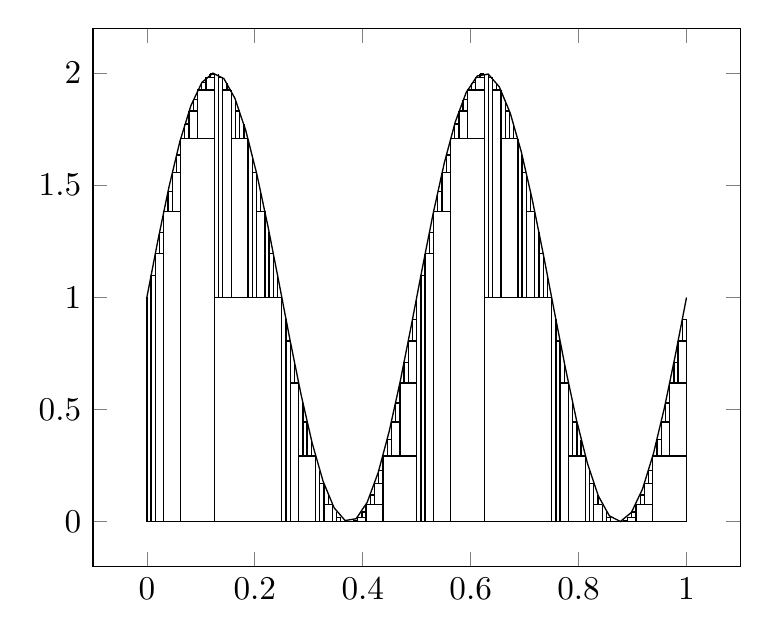
\begin{tikzpicture}[scale=1.2]
\begin{axis}
\addplot[domain=0:1, samples=50] {sin(4*pi*deg(x))+1};
\draw (axis cs: 0, 0) -- (axis cs: 1, 0);
\draw (axis cs: 1, 0) -- (axis cs: 1, 0.0);
\draw (axis cs: 0, 0) -- (axis cs: 0, 0.0);
\draw (axis cs: 1/2, 0) -- (axis cs: 1/2, 0.0);
\draw (axis cs: 1/2, 0) -- (axis cs: 1/2, 0.0);
\draw (axis cs: 1, 0) -- (axis cs: 1, 0.0);
\draw (axis cs: 1/2, 0.0) -- (axis cs: 1, 0.0);
\draw (axis cs: 0, 0) -- (axis cs: 0, 1.000000000236429);
\draw (axis cs: 1/4, 0) -- (axis cs: 1/4, 1.000000000236429);
\draw (axis cs: 1/4, 0) -- (axis cs: 1/4, 0.0);
\draw (axis cs: 1/2, 0) -- (axis cs: 1/2, 0.0);
\draw (axis cs: 1/4, 0.0) -- (axis cs: 1/2, 0.0);
\draw (axis cs: 1/2, 0.0) -- (axis cs: 1/2, 1.000000011107131);
\draw (axis cs: 3/4, 0.0) -- (axis cs: 3/4, 1.000000011107131);
\draw (axis cs: 3/4, 0.0) -- (axis cs: 3/4, 0.0);
\draw (axis cs: 1, 0.0) -- (axis cs: 1, 0.0);
\draw (axis cs: 3/4, 0.0) -- (axis cs: 1, 0.0);
\draw (axis cs: 0, 0) -- (axis cs: 0, 1.0000000001838258);
\draw (axis cs: 1/8, 0) -- (axis cs: 1/8, 1.0000000001838258);
\draw (axis cs: 1/8, 0) -- (axis cs: 1/8, 1.0000000055535658);
\draw (axis cs: 1/4, 0) -- (axis cs: 1/4, 1.0000000055535658);
\draw (axis cs: 1/8, 1.0000000055535658) -- (axis cs: 1/4, 1.0000000055535658);
\draw (axis cs: 1/4, 0.0) -- (axis cs: 1/4, 0.0);
\draw (axis cs: 3/8, 0.0) -- (axis cs: 3/8, 0.0);
\draw (axis cs: 3/8, 0.0) -- (axis cs: 3/8, 0.0);
\draw (axis cs: 1/2, 0.0) -- (axis cs: 1/2, 0.0);
\draw (axis cs: 3/8, 0.0) -- (axis cs: 1/2, 0.0);
\draw (axis cs: 1/2, 0.0) -- (axis cs: 1/2, 1.0000000081305724);
\draw (axis cs: 5/8, 0.0) -- (axis cs: 5/8, 1.0000000081305724);
\draw (axis cs: 5/8, 0.0) -- (axis cs: 5/8, 1.0000000139748395);
\draw (axis cs: 3/4, 0.0) -- (axis cs: 3/4, 1.0000000139748395);
\draw (axis cs: 5/8, 1.0000000139748395) -- (axis cs: 3/4, 1.0000000139748395);
\draw (axis cs: 3/4, 0.0) -- (axis cs: 3/4, 1.1102230246251565E-16);
\draw (axis cs: 7/8, 0.0) -- (axis cs: 7/8, 1.1102230246251565E-16);
\draw (axis cs: 7/8, 0.0) -- (axis cs: 7/8, 1.1102230246251565E-16);
\draw (axis cs: 1, 0.0) -- (axis cs: 1, 1.1102230246251565E-16);
\draw (axis cs: 7/8, 1.1102230246251565E-16) -- (axis cs: 1, 1.1102230246251565E-16);
\draw (axis cs: 0, 0) -- (axis cs: 0, 1.0000000002503824);
\draw (axis cs: 1/16, 0) -- (axis cs: 1/16, 1.0000000002503824);
\draw (axis cs: 1/16, 0) -- (axis cs: 1/16, 1.707106782400046);
\draw (axis cs: 1/8, 0) -- (axis cs: 1/8, 1.707106782400046);
\draw (axis cs: 1/16, 1.707106782400046) -- (axis cs: 1/8, 1.707106782400046);
\draw (axis cs: 1/8, 1.0000000055535658) -- (axis cs: 1/8, 1.7071067843635284);
\draw (axis cs: 3/16, 1.0000000055535658) -- (axis cs: 3/16, 1.7071067843635284);
\draw (axis cs: 3/16, 1.0000000055535658) -- (axis cs: 3/16, 1.000000004002456);
\draw (axis cs: 1/4, 1.0000000055535658) -- (axis cs: 1/4, 1.000000004002456);
\draw (axis cs: 3/16, 1.000000004002456) -- (axis cs: 1/4, 1.000000004002456);
\draw (axis cs: 1/4, 0.0) -- (axis cs: 1/4, 0.2928932239539149);
\draw (axis cs: 5/16, 0.0) -- (axis cs: 5/16, 0.2928932239539149);
\draw (axis cs: 5/16, 0.0) -- (axis cs: 5/16, 0.0);
\draw (axis cs: 3/8, 0.0) -- (axis cs: 3/8, 0.0);
\draw (axis cs: 5/16, 0.0) -- (axis cs: 3/8, 0.0);
\draw (axis cs: 3/8, 0.0) -- (axis cs: 3/8, 0.0);
\draw (axis cs: 7/16, 0.0) -- (axis cs: 7/16, 0.0);
\draw (axis cs: 7/16, 0.0) -- (axis cs: 7/16, 0.29289322315451494);
\draw (axis cs: 1/2, 0.0) -- (axis cs: 1/2, 0.29289322315451494);
\draw (axis cs: 7/16, 0.29289322315451494) -- (axis cs: 1/2, 0.29289322315451494);
\draw (axis cs: 1/2, 0.0) -- (axis cs: 1/2, 1.0000000117626413);
\draw (axis cs: 9/16, 0.0) -- (axis cs: 9/16, 1.0000000117626413);
\draw (axis cs: 9/16, 0.0) -- (axis cs: 9/16, 1.7071067895039909);
\draw (axis cs: 5/8, 0.0) -- (axis cs: 5/8, 1.7071067895039909);
\draw (axis cs: 9/16, 1.7071067895039909) -- (axis cs: 5/8, 1.7071067895039909);
\draw (axis cs: 5/8, 1.0000000139748395) -- (axis cs: 5/8, 1.707106788446632);
\draw (axis cs: 11/16, 1.0000000139748395) -- (axis cs: 11/16, 1.707106788446632);
\draw (axis cs: 11/16, 1.0000000139748395) -- (axis cs: 11/16, 1.000000019032353);
\draw (axis cs: 3/4, 1.0000000139748395) -- (axis cs: 3/4, 1.000000019032353);
\draw (axis cs: 11/16, 1.000000019032353) -- (axis cs: 3/4, 1.000000019032353);
\draw (axis cs: 3/4, 0.0) -- (axis cs: 3/4, 0.2928932322713579);
\draw (axis cs: 13/16, 0.0) -- (axis cs: 13/16, 0.2928932322713579);
\draw (axis cs: 13/16, 0.0) -- (axis cs: 13/16, 2.220446049250313E-16);
\draw (axis cs: 7/8, 0.0) -- (axis cs: 7/8, 2.220446049250313E-16);
\draw (axis cs: 13/16, 2.220446049250313E-16) -- (axis cs: 7/8, 2.220446049250313E-16);
\draw (axis cs: 7/8, 1.1102230246251565E-16) -- (axis cs: 7/8, 2.220446049250313E-16);
\draw (axis cs: 15/16, 1.1102230246251565E-16) -- (axis cs: 15/16, 2.220446049250313E-16);
\draw (axis cs: 15/16, 1.1102230246251565E-16) -- (axis cs: 15/16, 0.29289323216953733);
\draw (axis cs: 1, 1.1102230246251565E-16) -- (axis cs: 1, 0.29289323216953733);
\draw (axis cs: 15/16, 0.29289323216953733) -- (axis cs: 1, 0.29289323216953733);
\draw (axis cs: 0, 0) -- (axis cs: 0, 1.000000000202091);
\draw (axis cs: 1/32, 0) -- (axis cs: 1/32, 1.000000000202091);
\draw (axis cs: 1/32, 0) -- (axis cs: 1/32, 1.382683433157846);
\draw (axis cs: 1/16, 0) -- (axis cs: 1/16, 1.382683433157846);
\draw (axis cs: 1/32, 1.382683433157846) -- (axis cs: 1/16, 1.382683433157846);
\draw (axis cs: 1/16, 1.707106782400046) -- (axis cs: 1/16, 1.7071067821308197);
\draw (axis cs: 3/32, 1.707106782400046) -- (axis cs: 3/32, 1.7071067821308197);
\draw (axis cs: 3/32, 1.707106782400046) -- (axis cs: 3/32, 1.9238795333709715);
\draw (axis cs: 1/8, 1.707106782400046) -- (axis cs: 1/8, 1.9238795333709715);
\draw (axis cs: 3/32, 1.9238795333709715) -- (axis cs: 1/8, 1.9238795333709715);
\draw (axis cs: 1/8, 1.0000000055535658) -- (axis cs: 1/8, 1.9238795339022858);
\draw (axis cs: 5/32, 1.0000000055535658) -- (axis cs: 5/32, 1.9238795339022858);
\draw (axis cs: 5/32, 1.0000000055535658) -- (axis cs: 5/32, 1.7071067835903304);
\draw (axis cs: 3/16, 1.0000000055535658) -- (axis cs: 3/16, 1.7071067835903304);
\draw (axis cs: 5/32, 1.7071067835903304) -- (axis cs: 3/16, 1.7071067835903304);
\draw (axis cs: 3/16, 1.000000004002456) -- (axis cs: 3/16, 1.3826834351429769);
\draw (axis cs: 7/32, 1.000000004002456) -- (axis cs: 7/32, 1.3826834351429769);
\draw (axis cs: 7/32, 1.000000004002456) -- (axis cs: 7/32, 1.0000000058813205);
\draw (axis cs: 1/4, 1.000000004002456) -- (axis cs: 1/4, 1.0000000058813205);
\draw (axis cs: 7/32, 1.0000000058813205) -- (axis cs: 1/4, 1.0000000058813205);
\draw (axis cs: 1/4, 0.0) -- (axis cs: 1/4, 0.6173165730453525);
\draw (axis cs: 9/32, 0.0) -- (axis cs: 9/32, 0.6173165730453525);
\draw (axis cs: 9/32, 0.0) -- (axis cs: 9/32, 0.29289322267674545);
\draw (axis cs: 5/16, 0.0) -- (axis cs: 5/16, 0.29289322267674545);
\draw (axis cs: 9/32, 0.29289322267674545) -- (axis cs: 5/16, 0.29289322267674545);
\draw (axis cs: 5/16, 0.0) -- (axis cs: 5/16, 0.07612046942923334);
\draw (axis cs: 11/32, 0.0) -- (axis cs: 11/32, 0.07612046942923334);
\draw (axis cs: 11/32, 0.0) -- (axis cs: 11/32, 0.0);
\draw (axis cs: 3/8, 0.0) -- (axis cs: 3/8, 0.0);
\draw (axis cs: 11/32, 0.0) -- (axis cs: 3/8, 0.0);
\draw (axis cs: 3/8, 0.0) -- (axis cs: 3/8, 0.0);
\draw (axis cs: 13/32, 0.0) -- (axis cs: 13/32, 0.0);
\draw (axis cs: 13/32, 0.0) -- (axis cs: 13/32, 0.076120471130396);
\draw (axis cs: 7/16, 0.0) -- (axis cs: 7/16, 0.076120471130396);
\draw (axis cs: 13/32, 0.076120471130396) -- (axis cs: 7/16, 0.076120471130396);
\draw (axis cs: 7/16, 0.29289322315451494) -- (axis cs: 7/16, 0.29289322554240516);
\draw (axis cs: 15/32, 0.29289322315451494) -- (axis cs: 15/32, 0.29289322554240516);
\draw (axis cs: 15/32, 0.29289322315451494) -- (axis cs: 15/32, 0.6173165763021443);
\draw (axis cs: 1/2, 0.29289322315451494) -- (axis cs: 1/2, 0.6173165763021443);
\draw (axis cs: 15/32, 0.6173165763021443) -- (axis cs: 1/2, 0.6173165763021443);
\draw (axis cs: 1/2, 0.0) -- (axis cs: 1/2, 1.000000008988646);
\draw (axis cs: 17/32, 0.0) -- (axis cs: 17/32, 1.000000008988646);
\draw (axis cs: 17/32, 0.0) -- (axis cs: 17/32, 1.3826834403067085);
\draw (axis cs: 9/16, 0.0) -- (axis cs: 9/16, 1.3826834403067085);
\draw (axis cs: 17/32, 1.3826834403067085) -- (axis cs: 9/16, 1.3826834403067085);
\draw (axis cs: 9/16, 1.7071067895039909) -- (axis cs: 9/16, 1.7071067869871195);
\draw (axis cs: 19/32, 1.7071067895039909) -- (axis cs: 19/32, 1.7071067869871195);
\draw (axis cs: 19/32, 1.7071067895039909) -- (axis cs: 19/32, 1.923879535500254);
\draw (axis cs: 5/8, 1.7071067895039909) -- (axis cs: 5/8, 1.923879535500254);
\draw (axis cs: 19/32, 1.923879535500254) -- (axis cs: 5/8, 1.923879535500254);
\draw (axis cs: 5/8, 1.0000000139748395) -- (axis cs: 5/8, 1.9238795384036536);
\draw (axis cs: 21/32, 1.0000000139748395) -- (axis cs: 21/32, 1.9238795384036536);
\draw (axis cs: 21/32, 1.0000000139748395) -- (axis cs: 21/32, 1.7071067920742213);
\draw (axis cs: 11/16, 1.0000000139748395) -- (axis cs: 11/16, 1.7071067920742213);
\draw (axis cs: 21/32, 1.7071067920742213) -- (axis cs: 11/16, 1.7071067920742213);
\draw (axis cs: 11/16, 1.000000019032353) -- (axis cs: 11/16, 1.3826834465905207);
\draw (axis cs: 23/32, 1.000000019032353) -- (axis cs: 23/32, 1.3826834465905207);
\draw (axis cs: 23/32, 1.000000019032353) -- (axis cs: 23/32, 1.0000000153632311);
\draw (axis cs: 3/4, 1.000000019032353) -- (axis cs: 3/4, 1.0000000153632311);
\draw (axis cs: 23/32, 1.0000000153632311) -- (axis cs: 3/4, 1.0000000153632311);
\draw (axis cs: 3/4, 0.0) -- (axis cs: 3/4, 0.6173165814658779);
\draw (axis cs: 25/32, 0.0) -- (axis cs: 25/32, 0.6173165814658779);
\draw (axis cs: 25/32, 0.0) -- (axis cs: 25/32, 0.2928932291215375);
\draw (axis cs: 13/16, 0.0) -- (axis cs: 13/16, 0.2928932291215375);
\draw (axis cs: 25/32, 0.2928932291215375) -- (axis cs: 13/16, 0.2928932291215375);
\draw (axis cs: 13/16, 2.220446049250313E-16) -- (axis cs: 13/16, 0.07612047291712909);
\draw (axis cs: 27/32, 2.220446049250313E-16) -- (axis cs: 27/32, 0.07612047291712909);
\draw (axis cs: 27/32, 2.220446049250313E-16) -- (axis cs: 27/32, 1.1102230246251565E-16);
\draw (axis cs: 7/8, 2.220446049250313E-16) -- (axis cs: 7/8, 1.1102230246251565E-16);
\draw (axis cs: 27/32, 1.1102230246251565E-16) -- (axis cs: 7/8, 1.1102230246251565E-16);
\draw (axis cs: 7/8, 1.1102230246251565E-16) -- (axis cs: 7/8, 1.1102230246251565E-16);
\draw (axis cs: 29/32, 1.1102230246251565E-16) -- (axis cs: 29/32, 1.1102230246251565E-16);
\draw (axis cs: 29/32, 1.1102230246251565E-16) -- (axis cs: 29/32, 0.07612047261656973);
\draw (axis cs: 15/16, 1.1102230246251565E-16) -- (axis cs: 15/16, 0.07612047261656973);
\draw (axis cs: 29/32, 0.07612047261656973) -- (axis cs: 15/16, 0.07612047261656973);
\draw (axis cs: 15/16, 0.29289323216953733) -- (axis cs: 15/16, 0.29289322801081585);
\draw (axis cs: 31/32, 0.29289323216953733) -- (axis cs: 31/32, 0.29289322801081585);
\draw (axis cs: 31/32, 0.29289323216953733) -- (axis cs: 31/32, 0.617316579289038);
\draw (axis cs: 1, 0.29289323216953733) -- (axis cs: 1, 0.617316579289038);
\draw (axis cs: 31/32, 0.617316579289038) -- (axis cs: 1, 0.617316579289038);
\draw (axis cs: 0, 0) -- (axis cs: 0, 1.0000000001394955);
\draw (axis cs: 1/64, 0) -- (axis cs: 1/64, 1.0000000001394955);
\draw (axis cs: 1/64, 0) -- (axis cs: 1/64, 1.1950903223811593);
\draw (axis cs: 1/32, 0) -- (axis cs: 1/32, 1.1950903223811593);
\draw (axis cs: 1/64, 1.1950903223811593) -- (axis cs: 1/32, 1.1950903223811593);
\draw (axis cs: 1/32, 1.382683433157846) -- (axis cs: 1/32, 1.3826834329239164);
\draw (axis cs: 3/64, 1.382683433157846) -- (axis cs: 3/64, 1.3826834329239164);
\draw (axis cs: 3/64, 1.382683433157846) -- (axis cs: 3/64, 1.5555702339364768);
\draw (axis cs: 1/16, 1.382683433157846) -- (axis cs: 1/16, 1.5555702339364768);
\draw (axis cs: 3/64, 1.5555702339364768) -- (axis cs: 1/16, 1.5555702339364768);
\draw (axis cs: 1/16, 1.707106782400046) -- (axis cs: 1/16, 1.707106782471663);
\draw (axis cs: 5/64, 1.707106782400046) -- (axis cs: 5/64, 1.707106782471663);
\draw (axis cs: 5/64, 1.707106782400046) -- (axis cs: 5/64, 1.831469613312254);
\draw (axis cs: 3/32, 1.707106782400046) -- (axis cs: 3/32, 1.831469613312254);
\draw (axis cs: 5/64, 1.831469613312254) -- (axis cs: 3/32, 1.831469613312254);
\draw (axis cs: 3/32, 1.9238795333709715) -- (axis cs: 3/32, 1.923879533137701);
\draw (axis cs: 7/64, 1.9238795333709715) -- (axis cs: 7/64, 1.923879533137701);
\draw (axis cs: 7/64, 1.9238795333709715) -- (axis cs: 7/64, 1.9807852809769249);
\draw (axis cs: 1/8, 1.9238795333709715) -- (axis cs: 1/8, 1.9807852809769249);
\draw (axis cs: 7/64, 1.9807852809769249) -- (axis cs: 1/8, 1.9807852809769249);
\draw (axis cs: 1/8, 1.0000000055535658) -- (axis cs: 1/8, 1.9807852809622184);
\draw (axis cs: 9/64, 1.0000000055535658) -- (axis cs: 9/64, 1.9807852809622184);
\draw (axis cs: 9/64, 1.0000000055535658) -- (axis cs: 9/64, 1.9238795335326417);
\draw (axis cs: 5/32, 1.0000000055535658) -- (axis cs: 5/32, 1.9238795335326417);
\draw (axis cs: 9/64, 1.9238795335326417) -- (axis cs: 5/32, 1.9238795335326417);
\draw (axis cs: 5/32, 1.7071067835903304) -- (axis cs: 5/32, 1.831469613676237);
\draw (axis cs: 11/64, 1.7071067835903304) -- (axis cs: 11/64, 1.831469613676237);
\draw (axis cs: 11/64, 1.7071067835903304) -- (axis cs: 11/64, 1.707106784551024);
\draw (axis cs: 3/16, 1.7071067835903304) -- (axis cs: 3/16, 1.707106784551024);
\draw (axis cs: 11/64, 1.707106784551024) -- (axis cs: 3/16, 1.707106784551024);
\draw (axis cs: 3/16, 1.000000004002456) -- (axis cs: 3/16, 1.5555702369758078);
\draw (axis cs: 13/64, 1.000000004002456) -- (axis cs: 13/64, 1.5555702369758078);
\draw (axis cs: 13/64, 1.000000004002456) -- (axis cs: 13/64, 1.3826834367609901);
\draw (axis cs: 7/32, 1.000000004002456) -- (axis cs: 7/32, 1.3826834367609901);
\draw (axis cs: 13/64, 1.3826834367609901) -- (axis cs: 7/32, 1.3826834367609901);
\draw (axis cs: 7/32, 1.0000000058813205) -- (axis cs: 7/32, 1.1950903265550472);
\draw (axis cs: 15/64, 1.0000000058813205) -- (axis cs: 15/64, 1.1950903265550472);
\draw (axis cs: 15/64, 1.0000000058813205) -- (axis cs: 15/64, 1.0000000044314918);
\draw (axis cs: 1/4, 1.0000000058813205) -- (axis cs: 1/4, 1.0000000044314918);
\draw (axis cs: 15/64, 1.0000000044314918) -- (axis cs: 1/4, 1.0000000044314918);
\draw (axis cs: 1/4, 0.0) -- (axis cs: 1/4, 0.8049096821376361);
\draw (axis cs: 17/64, 0.0) -- (axis cs: 17/64, 0.8049096821376361);
\draw (axis cs: 17/64, 0.0) -- (axis cs: 17/64, 0.6173165713662676);
\draw (axis cs: 9/32, 0.0) -- (axis cs: 9/32, 0.6173165713662676);
\draw (axis cs: 17/64, 0.6173165713662676) -- (axis cs: 9/32, 0.6173165713662676);
\draw (axis cs: 9/32, 0.29289322267674545) -- (axis cs: 9/32, 0.44442977338167267);
\draw (axis cs: 19/64, 0.29289322267674545) -- (axis cs: 19/64, 0.44442977338167267);
\draw (axis cs: 19/64, 0.29289322267674545) -- (axis cs: 19/64, 0.2928932242572895);
\draw (axis cs: 5/16, 0.29289322267674545) -- (axis cs: 5/16, 0.2928932242572895);
\draw (axis cs: 19/64, 0.2928932242572895) -- (axis cs: 5/16, 0.2928932242572895);
\draw (axis cs: 5/16, 0.0) -- (axis cs: 5/16, 0.16853039197465014);
\draw (axis cs: 21/64, 0.0) -- (axis cs: 21/64, 0.16853039197465014);
\draw (axis cs: 21/64, 0.0) -- (axis cs: 21/64, 0.07612047043489656);
\draw (axis cs: 11/32, 0.0) -- (axis cs: 11/32, 0.07612047043489656);
\draw (axis cs: 21/64, 0.07612047043489656) -- (axis cs: 11/32, 0.07612047043489656);
\draw (axis cs: 11/32, 0.0) -- (axis cs: 11/32, 0.0192147210987208);
\draw (axis cs: 23/64, 0.0) -- (axis cs: 23/64, 0.0192147210987208);
\draw (axis cs: 23/64, 0.0) -- (axis cs: 23/64, 0.0);
\draw (axis cs: 3/8, 0.0) -- (axis cs: 3/8, 0.0);
\draw (axis cs: 23/64, 0.0) -- (axis cs: 3/8, 0.0);
\draw (axis cs: 3/8, 0.0) -- (axis cs: 3/8, 0.0);
\draw (axis cs: 25/64, 0.0) -- (axis cs: 25/64, 0.0);
\draw (axis cs: 25/64, 0.0) -- (axis cs: 25/64, 0.019214721044814476);
\draw (axis cs: 13/32, 0.0) -- (axis cs: 13/32, 0.019214721044814476);
\draw (axis cs: 25/64, 0.019214721044814476) -- (axis cs: 13/32, 0.019214721044814476);
\draw (axis cs: 13/32, 0.076120471130396) -- (axis cs: 13/32, 0.07612047025401592);
\draw (axis cs: 27/64, 0.076120471130396) -- (axis cs: 27/64, 0.07612047025401592);
\draw (axis cs: 27/64, 0.076120471130396) -- (axis cs: 27/64, 0.168530391602966);
\draw (axis cs: 7/16, 0.076120471130396) -- (axis cs: 7/16, 0.168530391602966);
\draw (axis cs: 27/64, 0.168530391602966) -- (axis cs: 7/16, 0.168530391602966);
\draw (axis cs: 7/16, 0.29289322315451494) -- (axis cs: 7/16, 0.2928932236453855);
\draw (axis cs: 29/64, 0.29289322315451494) -- (axis cs: 29/64, 0.2928932236453855);
\draw (axis cs: 29/64, 0.29289322315451494) -- (axis cs: 29/64, 0.4444297724988914);
\draw (axis cs: 15/32, 0.29289322315451494) -- (axis cs: 15/32, 0.4444297724988914);
\draw (axis cs: 29/64, 0.4444297724988914) -- (axis cs: 15/32, 0.4444297724988914);
\draw (axis cs: 15/32, 0.6173165763021443) -- (axis cs: 15/32, 0.6173165735853278);
\draw (axis cs: 31/64, 0.6173165763021443) -- (axis cs: 31/64, 0.6173165735853278);
\draw (axis cs: 31/64, 0.6173165763021443) -- (axis cs: 31/64, 0.8049096841082247);
\draw (axis cs: 1/2, 0.6173165763021443) -- (axis cs: 1/2, 0.8049096841082247);
\draw (axis cs: 31/64, 0.8049096841082247) -- (axis cs: 1/2, 0.8049096841082247);
\draw (axis cs: 1/2, 0.0) -- (axis cs: 1/2, 1.0000000124568353);
\draw (axis cs: 33/64, 0.0) -- (axis cs: 33/64, 1.0000000124568353);
\draw (axis cs: 33/64, 0.0) -- (axis cs: 33/64, 1.1950903342336092);
\draw (axis cs: 17/32, 0.0) -- (axis cs: 17/32, 1.1950903342336092);
\draw (axis cs: 33/64, 1.1950903342336092) -- (axis cs: 17/32, 1.1950903342336092);
\draw (axis cs: 17/32, 1.3826834403067085) -- (axis cs: 17/32, 1.3826834438737055);
\draw (axis cs: 35/64, 1.3826834403067085) -- (axis cs: 35/64, 1.3826834438737055);
\draw (axis cs: 35/64, 1.3826834403067085) -- (axis cs: 35/64, 1.5555702433770828);
\draw (axis cs: 9/16, 1.3826834403067085) -- (axis cs: 9/16, 1.5555702433770828);
\draw (axis cs: 35/64, 1.5555702433770828) -- (axis cs: 9/16, 1.5555702433770828);
\draw (axis cs: 9/16, 1.7071067895039909) -- (axis cs: 9/16, 1.7071067899948602);
\draw (axis cs: 37/64, 1.7071067895039909) -- (axis cs: 37/64, 1.7071067899948602);
\draw (axis cs: 37/64, 1.7071067895039909) -- (axis cs: 37/64, 1.831469619223192);
\draw (axis cs: 19/32, 1.7071067895039909) -- (axis cs: 19/32, 1.831469619223192);
\draw (axis cs: 37/64, 1.831469619223192) -- (axis cs: 19/32, 1.831469619223192);
\draw (axis cs: 19/32, 1.923879535500254) -- (axis cs: 19/32, 1.9238795372783113);
\draw (axis cs: 39/64, 1.923879535500254) -- (axis cs: 39/64, 1.9238795372783113);
\draw (axis cs: 39/64, 1.923879535500254) -- (axis cs: 39/64, 1.980785282816944);
\draw (axis cs: 5/8, 1.923879535500254) -- (axis cs: 5/8, 1.980785282816944);
\draw (axis cs: 39/64, 1.980785282816944) -- (axis cs: 5/8, 1.980785282816944);
\draw (axis cs: 5/8, 1.0000000139748395) -- (axis cs: 5/8, 1.9807852827403325);
\draw (axis cs: 41/64, 1.0000000139748395) -- (axis cs: 41/64, 1.9807852827403325);
\draw (axis cs: 41/64, 1.0000000139748395) -- (axis cs: 41/64, 1.9238795370205377);
\draw (axis cs: 21/32, 1.0000000139748395) -- (axis cs: 21/32, 1.9238795370205377);
\draw (axis cs: 41/64, 1.9238795370205377) -- (axis cs: 21/32, 1.9238795370205377);
\draw (axis cs: 21/32, 1.7071067920742213) -- (axis cs: 21/32, 1.8314696187398765);
\draw (axis cs: 43/64, 1.7071067920742213) -- (axis cs: 43/64, 1.8314696187398765);
\draw (axis cs: 43/64, 1.7071067920742213) -- (axis cs: 43/64, 1.7071067892408764);
\draw (axis cs: 11/16, 1.7071067920742213) -- (axis cs: 11/16, 1.7071067892408764);
\draw (axis cs: 43/64, 1.7071067892408764) -- (axis cs: 11/16, 1.7071067892408764);
\draw (axis cs: 11/16, 1.000000019032353) -- (axis cs: 11/16, 1.5555702423272328);
\draw (axis cs: 45/64, 1.000000019032353) -- (axis cs: 45/64, 1.5555702423272328);
\draw (axis cs: 45/64, 1.000000019032353) -- (axis cs: 45/64, 1.3826834425257721);
\draw (axis cs: 23/32, 1.000000019032353) -- (axis cs: 23/32, 1.3826834425257721);
\draw (axis cs: 45/64, 1.3826834425257721) -- (axis cs: 23/32, 1.3826834425257721);
\draw (axis cs: 23/32, 1.0000000153632311) -- (axis cs: 23/32, 1.1950903326100732);
\draw (axis cs: 47/64, 1.0000000153632311) -- (axis cs: 47/64, 1.1950903326100732);
\draw (axis cs: 47/64, 1.0000000153632311) -- (axis cs: 47/64, 1.0000000106051439);
\draw (axis cs: 3/4, 1.0000000153632311) -- (axis cs: 3/4, 1.0000000106051439);
\draw (axis cs: 47/64, 1.0000000106051439) -- (axis cs: 3/4, 1.0000000106051439);
\draw (axis cs: 3/4, 0.0) -- (axis cs: 3/4, 0.8049096881926627);
\draw (axis cs: 49/64, 0.0) -- (axis cs: 49/64, 0.8049096881926627);
\draw (axis cs: 49/64, 0.0) -- (axis cs: 49/64, 0.6173165770699784);
\draw (axis cs: 25/32, 0.0) -- (axis cs: 25/32, 0.6173165770699784);
\draw (axis cs: 49/64, 0.6173165770699784) -- (axis cs: 25/32, 0.6173165770699784);
\draw (axis cs: 25/32, 0.2928932291215375) -- (axis cs: 25/32, 0.44442978373915387);
\draw (axis cs: 51/64, 0.2928932291215375) -- (axis cs: 51/64, 0.44442978373915387);
\draw (axis cs: 51/64, 0.2928932291215375) -- (axis cs: 51/64, 0.29289323306560355);
\draw (axis cs: 13/16, 0.2928932291215375) -- (axis cs: 13/16, 0.29289323306560355);
\draw (axis cs: 51/64, 0.29289323306560355) -- (axis cs: 13/16, 0.29289323306560355);
\draw (axis cs: 13/16, 2.220446049250313E-16) -- (axis cs: 13/16, 0.16853039889529742);
\draw (axis cs: 53/64, 2.220446049250313E-16) -- (axis cs: 53/64, 0.16853039889529742);
\draw (axis cs: 53/64, 2.220446049250313E-16) -- (axis cs: 53/64, 0.07612047520192178);
\draw (axis cs: 27/32, 2.220446049250313E-16) -- (axis cs: 27/32, 0.07612047520192178);
\draw (axis cs: 53/64, 0.07612047520192178) -- (axis cs: 27/32, 0.07612047520192178);
\draw (axis cs: 27/32, 1.1102230246251565E-16) -- (axis cs: 27/32, 0.01921472352892939);
\draw (axis cs: 55/64, 1.1102230246251565E-16) -- (axis cs: 55/64, 0.01921472352892939);
\draw (axis cs: 55/64, 1.1102230246251565E-16) -- (axis cs: 55/64, 2.220446049250313E-16);
\draw (axis cs: 7/8, 1.1102230246251565E-16) -- (axis cs: 7/8, 2.220446049250313E-16);
\draw (axis cs: 55/64, 2.220446049250313E-16) -- (axis cs: 7/8, 2.220446049250313E-16);
\draw (axis cs: 7/8, 1.1102230246251565E-16) -- (axis cs: 7/8, 2.220446049250313E-16);
\draw (axis cs: 57/64, 1.1102230246251565E-16) -- (axis cs: 57/64, 2.220446049250313E-16);
\draw (axis cs: 57/64, 1.1102230246251565E-16) -- (axis cs: 57/64, 0.01921472352892928);
\draw (axis cs: 29/32, 1.1102230246251565E-16) -- (axis cs: 29/32, 0.01921472352892928);
\draw (axis cs: 57/64, 0.01921472352892928) -- (axis cs: 29/32, 0.01921472352892928);
\draw (axis cs: 29/32, 0.07612047261656973) -- (axis cs: 29/32, 0.07612047520192144);
\draw (axis cs: 59/64, 0.07612047261656973) -- (axis cs: 59/64, 0.07612047520192144);
\draw (axis cs: 59/64, 0.07612047261656973) -- (axis cs: 59/64, 0.16853039889529697);
\draw (axis cs: 15/16, 0.07612047261656973) -- (axis cs: 15/16, 0.16853039889529697);
\draw (axis cs: 59/64, 0.16853039889529697) -- (axis cs: 15/16, 0.16853039889529697);
\draw (axis cs: 15/16, 0.29289323216953733) -- (axis cs: 15/16, 0.292893233065603);
\draw (axis cs: 61/64, 0.29289323216953733) -- (axis cs: 61/64, 0.292893233065603);
\draw (axis cs: 61/64, 0.29289323216953733) -- (axis cs: 61/64, 0.4444297837391532);
\draw (axis cs: 31/32, 0.29289323216953733) -- (axis cs: 31/32, 0.4444297837391532);
\draw (axis cs: 61/64, 0.4444297837391532) -- (axis cs: 31/32, 0.4444297837391532);
\draw (axis cs: 31/32, 0.617316579289038) -- (axis cs: 31/32, 0.6173165862562409);
\draw (axis cs: 63/64, 0.617316579289038) -- (axis cs: 63/64, 0.6173165862562409);
\draw (axis cs: 63/64, 0.617316579289038) -- (axis cs: 63/64, 0.8049096977140695);
\draw (axis cs: 1, 0.617316579289038) -- (axis cs: 1, 0.8049096977140695);
\draw (axis cs: 63/64, 0.8049096977140695) -- (axis cs: 1, 0.8049096977140695);
\draw (axis cs: 0, 0) -- (axis cs: 0, 1.0000000002145182);
\draw (axis cs: 1/128, 0) -- (axis cs: 1/128, 1.0000000002145182);
\draw (axis cs: 1/128, 0) -- (axis cs: 1/128, 1.0980171406657118);
\draw (axis cs: 1/64, 0) -- (axis cs: 1/64, 1.0980171406657118);
\draw (axis cs: 1/128, 1.0980171406657118) -- (axis cs: 1/64, 1.0980171406657118);
\draw (axis cs: 1/64, 1.1950903223811593) -- (axis cs: 1/64, 1.1950903225669531);
\draw (axis cs: 3/128, 1.1950903223811593) -- (axis cs: 3/128, 1.1950903225669531);
\draw (axis cs: 3/128, 1.1950903223811593) -- (axis cs: 3/128, 1.2902846777219525);
\draw (axis cs: 1/32, 1.1950903223811593) -- (axis cs: 1/32, 1.2902846777219525);
\draw (axis cs: 3/128, 1.2902846777219525) -- (axis cs: 1/32, 1.2902846777219525);
\draw (axis cs: 1/32, 1.382683433157846) -- (axis cs: 1/32, 1.3826834332046318);
\draw (axis cs: 5/128, 1.382683433157846) -- (axis cs: 5/128, 1.3826834332046318);
\draw (axis cs: 5/128, 1.382683433157846) -- (axis cs: 5/128, 1.4713967375789754);
\draw (axis cs: 3/64, 1.382683433157846) -- (axis cs: 3/64, 1.4713967375789754);
\draw (axis cs: 5/128, 1.4713967375789754) -- (axis cs: 3/64, 1.4713967375789754);
\draw (axis cs: 3/64, 1.5555702339364768) -- (axis cs: 3/64, 1.5555702336478754);
\draw (axis cs: 7/128, 1.5555702339364768) -- (axis cs: 7/128, 1.5555702336478754);
\draw (axis cs: 7/128, 1.5555702339364768) -- (axis cs: 7/128, 1.6343932853002259);
\draw (axis cs: 1/16, 1.5555702339364768) -- (axis cs: 1/16, 1.6343932853002259);
\draw (axis cs: 7/128, 1.6343932853002259) -- (axis cs: 1/16, 1.6343932853002259);
\draw (axis cs: 1/16, 1.707106782400046) -- (axis cs: 1/16, 1.7071067822245676);
\draw (axis cs: 9/128, 1.707106782400046) -- (axis cs: 9/128, 1.7071067822245676);
\draw (axis cs: 9/128, 1.707106782400046) -- (axis cs: 9/128, 1.7730104542317335);
\draw (axis cs: 5/64, 1.707106782400046) -- (axis cs: 5/64, 1.7730104542317335);
\draw (axis cs: 9/128, 1.7730104542317335) -- (axis cs: 5/64, 1.7730104542317335);
\draw (axis cs: 5/64, 1.831469613312254) -- (axis cs: 5/64, 1.8314696130090264);
\draw (axis cs: 11/128, 1.831469613312254) -- (axis cs: 11/128, 1.8314696130090264);
\draw (axis cs: 11/128, 1.831469613312254) -- (axis cs: 11/128, 1.8819212654698285);
\draw (axis cs: 3/32, 1.831469613312254) -- (axis cs: 3/32, 1.8819212654698285);
\draw (axis cs: 11/128, 1.8819212654698285) -- (axis cs: 3/32, 1.8819212654698285);
\draw (axis cs: 3/32, 1.9238795333709715) -- (axis cs: 3/32, 1.9238795334217076);
\draw (axis cs: 13/128, 1.9238795333709715) -- (axis cs: 13/128, 1.9238795334217076);
\draw (axis cs: 13/128, 1.9238795333709715) -- (axis cs: 13/128, 1.9569403364228088);
\draw (axis cs: 7/64, 1.9238795333709715) -- (axis cs: 7/64, 1.9569403364228088);
\draw (axis cs: 13/128, 1.9569403364228088) -- (axis cs: 7/64, 1.9569403364228088);
\draw (axis cs: 7/64, 1.9807852809769249) -- (axis cs: 7/64, 1.9807852808615491);
\draw (axis cs: 15/128, 1.9807852809769249) -- (axis cs: 15/128, 1.9807852808615491);
\draw (axis cs: 15/128, 1.9807852809769249) -- (axis cs: 15/128, 1.9951847268928422);
\draw (axis cs: 1/8, 1.9807852809769249) -- (axis cs: 1/8, 1.9951847268928422);
\draw (axis cs: 15/128, 1.9951847268928422) -- (axis cs: 1/8, 1.9951847268928422);
\draw (axis cs: 1/8, 1.0000000055535658) -- (axis cs: 1/8, 1.9951847268735965);
\draw (axis cs: 17/128, 1.0000000055535658) -- (axis cs: 17/128, 1.9951847268735965);
\draw (axis cs: 17/128, 1.0000000055535658) -- (axis cs: 17/128, 1.980785280784937);
\draw (axis cs: 9/64, 1.0000000055535658) -- (axis cs: 9/64, 1.980785280784937);
\draw (axis cs: 17/128, 1.980785280784937) -- (axis cs: 9/64, 1.980785280784937);
\draw (axis cs: 9/64, 1.9238795335326417) -- (axis cs: 9/64, 1.9569403368496232);
\draw (axis cs: 19/128, 1.9238795335326417) -- (axis cs: 19/128, 1.9569403368496232);
\draw (axis cs: 19/128, 1.9238795335326417) -- (axis cs: 19/128, 1.9238795339843784);
\draw (axis cs: 5/32, 1.9238795335326417) -- (axis cs: 5/32, 1.9238795339843784);
\draw (axis cs: 19/128, 1.9238795339843784) -- (axis cs: 5/32, 1.9238795339843784);
\draw (axis cs: 5/32, 1.7071067835903304) -- (axis cs: 5/32, 1.8819212661629374);
\draw (axis cs: 21/128, 1.7071067835903304) -- (axis cs: 21/128, 1.8819212661629374);
\draw (axis cs: 21/128, 1.7071067835903304) -- (axis cs: 21/128, 1.8314696144411429);
\draw (axis cs: 11/64, 1.7071067835903304) -- (axis cs: 11/64, 1.8314696144411429);
\draw (axis cs: 21/128, 1.8314696144411429) -- (axis cs: 11/64, 1.8314696144411429);
\draw (axis cs: 11/64, 1.707106784551024) -- (axis cs: 11/64, 1.773010455801811);
\draw (axis cs: 23/128, 1.707106784551024) -- (axis cs: 23/128, 1.773010455801811);
\draw (axis cs: 23/128, 1.707106784551024) -- (axis cs: 23/128, 1.7071067838357656);
\draw (axis cs: 3/16, 1.707106784551024) -- (axis cs: 3/16, 1.7071067838357656);
\draw (axis cs: 23/128, 1.7071067838357656) -- (axis cs: 3/16, 1.7071067838357656);
\draw (axis cs: 3/16, 1.000000004002456) -- (axis cs: 3/16, 1.6343932869838853);
\draw (axis cs: 25/128, 1.000000004002456) -- (axis cs: 25/128, 1.6343932869838853);
\draw (axis cs: 25/128, 1.000000004002456) -- (axis cs: 25/128, 1.5555702359714942);
\draw (axis cs: 13/64, 1.000000004002456) -- (axis cs: 13/64, 1.5555702359714942);
\draw (axis cs: 25/128, 1.5555702359714942) -- (axis cs: 13/64, 1.5555702359714942);
\draw (axis cs: 13/64, 1.3826834367609901) -- (axis cs: 13/64, 1.4713967398704213);
\draw (axis cs: 27/128, 1.3826834367609901) -- (axis cs: 27/128, 1.4713967398704213);
\draw (axis cs: 27/128, 1.3826834367609901) -- (axis cs: 27/128, 1.3826834354636532);
\draw (axis cs: 7/32, 1.3826834367609901) -- (axis cs: 7/32, 1.3826834354636532);
\draw (axis cs: 27/128, 1.3826834354636532) -- (axis cs: 7/32, 1.3826834354636532);
\draw (axis cs: 7/32, 1.0000000058813205) -- (axis cs: 7/32, 1.2902846803699597);
\draw (axis cs: 29/128, 1.0000000058813205) -- (axis cs: 29/128, 1.2902846803699597);
\draw (axis cs: 29/128, 1.0000000058813205) -- (axis cs: 29/128, 1.195090325112969);
\draw (axis cs: 15/64, 1.0000000058813205) -- (axis cs: 15/64, 1.195090325112969);
\draw (axis cs: 29/128, 1.195090325112969) -- (axis cs: 15/64, 1.195090325112969);
\draw (axis cs: 15/64, 1.0000000044314918) -- (axis cs: 15/64, 1.098017146527987);
\draw (axis cs: 31/128, 1.0000000044314918) -- (axis cs: 31/128, 1.098017146527987);
\draw (axis cs: 31/128, 1.0000000044314918) -- (axis cs: 31/128, 1.000000006228418);
\draw (axis cs: 1/4, 1.0000000044314918) -- (axis cs: 1/4, 1.000000006228418);
\draw (axis cs: 31/128, 1.000000006228418) -- (axis cs: 1/4, 1.000000006228418);
\draw (axis cs: 1/4, 0.0) -- (axis cs: 1/4, 0.9019828658688661);
\draw (axis cs: 33/128, 0.0) -- (axis cs: 33/128, 0.9019828658688661);
\draw (axis cs: 33/128, 0.0) -- (axis cs: 33/128, 0.8049096840926125);
\draw (axis cs: 17/64, 0.0) -- (axis cs: 17/64, 0.8049096840926125);
\draw (axis cs: 33/128, 0.8049096840926125) -- (axis cs: 17/64, 0.8049096840926125);
\draw (axis cs: 17/64, 0.6173165713662676) -- (axis cs: 17/64, 0.709715328705762);
\draw (axis cs: 35/128, 0.6173165713662676) -- (axis cs: 35/128, 0.709715328705762);
\draw (axis cs: 35/128, 0.6173165713662676) -- (axis cs: 35/128, 0.6173165733892181);
\draw (axis cs: 9/32, 0.6173165713662676) -- (axis cs: 9/32, 0.6173165733892181);
\draw (axis cs: 35/128, 0.6173165733892181) -- (axis cs: 9/32, 0.6173165733892181);
\draw (axis cs: 9/32, 0.29289322267674545) -- (axis cs: 9/32, 0.5286032686669768);
\draw (axis cs: 37/128, 0.29289322267674545) -- (axis cs: 37/128, 0.5286032686669768);
\draw (axis cs: 37/128, 0.29289322267674545) -- (axis cs: 37/128, 0.444429772153375);
\draw (axis cs: 19/64, 0.29289322267674545) -- (axis cs: 19/64, 0.444429772153375);
\draw (axis cs: 37/128, 0.444429772153375) -- (axis cs: 19/64, 0.444429772153375);
\draw (axis cs: 19/64, 0.2928932242572895) -- (axis cs: 19/64, 0.365606720569739);
\draw (axis cs: 39/128, 0.2928932242572895) -- (axis cs: 39/128, 0.365606720569739);
\draw (axis cs: 39/128, 0.2928932242572895) -- (axis cs: 39/128, 0.292893223073868);
\draw (axis cs: 5/16, 0.2928932242572895) -- (axis cs: 5/16, 0.292893223073868);
\draw (axis cs: 39/128, 0.292893223073868) -- (axis cs: 5/16, 0.292893223073868);
\draw (axis cs: 5/16, 0.0) -- (axis cs: 5/16, 0.22698955039728885);
\draw (axis cs: 41/128, 0.0) -- (axis cs: 41/128, 0.22698955039728885);
\draw (axis cs: 41/128, 0.0) -- (axis cs: 41/128, 0.1685303909357564);
\draw (axis cs: 21/64, 0.0) -- (axis cs: 21/64, 0.1685303909357564);
\draw (axis cs: 41/128, 0.1685303909357564) -- (axis cs: 21/64, 0.1685303909357564);
\draw (axis cs: 21/64, 0.07612047043489656) -- (axis cs: 21/64, 0.1180787383530375);
\draw (axis cs: 43/128, 0.07612047043489656) -- (axis cs: 43/128, 0.1180787383530375);
\draw (axis cs: 43/128, 0.07612047043489656) -- (axis cs: 43/128, 0.07612046964415442);
\draw (axis cs: 11/32, 0.07612047043489656) -- (axis cs: 11/32, 0.07612046964415442);
\draw (axis cs: 43/128, 0.07612046964415442) -- (axis cs: 11/32, 0.07612046964415442);
\draw (axis cs: 11/32, 0.0) -- (axis cs: 11/32, 0.0430596658743031);
\draw (axis cs: 45/128, 0.0) -- (axis cs: 45/128, 0.0430596658743031);
\draw (axis cs: 45/128, 0.0) -- (axis cs: 45/128, 0.019214720657298012);
\draw (axis cs: 23/64, 0.0) -- (axis cs: 23/64, 0.019214720657298012);
\draw (axis cs: 45/128, 0.019214720657298012) -- (axis cs: 23/64, 0.019214720657298012);
\draw (axis cs: 23/64, 0.0) -- (axis cs: 23/64, 0.0048152738510102155);
\draw (axis cs: 47/128, 0.0) -- (axis cs: 47/128, 0.0048152738510102155);
\draw (axis cs: 47/128, 0.0) -- (axis cs: 47/128, 0.0);
\draw (axis cs: 3/8, 0.0) -- (axis cs: 3/8, 0.0);
\draw (axis cs: 47/128, 0.0) -- (axis cs: 3/8, 0.0);
\draw (axis cs: 3/8, 0.0) -- (axis cs: 3/8, 0.0);
\draw (axis cs: 49/128, 0.0) -- (axis cs: 49/128, 0.0);
\draw (axis cs: 49/128, 0.0) -- (axis cs: 49/128, 0.004815273831764499);
\draw (axis cs: 25/64, 0.0) -- (axis cs: 25/64, 0.004815273831764499);
\draw (axis cs: 49/128, 0.004815273831764499) -- (axis cs: 25/64, 0.004815273831764499);
\draw (axis cs: 25/64, 0.019214721044814476) -- (axis cs: 25/64, 0.019214720580686073);
\draw (axis cs: 51/128, 0.019214721044814476) -- (axis cs: 51/128, 0.019214720580686073);
\draw (axis cs: 51/128, 0.019214721044814476) -- (axis cs: 51/128, 0.04305966719321963);
\draw (axis cs: 13/32, 0.019214721044814476) -- (axis cs: 13/32, 0.04305966719321963);
\draw (axis cs: 51/128, 0.04305966719321963) -- (axis cs: 13/32, 0.04305966719321963);
\draw (axis cs: 13/32, 0.076120471130396) -- (axis cs: 13/32, 0.07612047134531741);
\draw (axis cs: 53/128, 0.076120471130396) -- (axis cs: 53/128, 0.07612047134531741);
\draw (axis cs: 53/128, 0.076120471130396) -- (axis cs: 53/128, 0.11807874040228317);
\draw (axis cs: 27/64, 0.076120471130396) -- (axis cs: 27/64, 0.11807874040228317);
\draw (axis cs: 53/128, 0.11807874040228317) -- (axis cs: 27/64, 0.11807874040228317);
\draw (axis cs: 27/64, 0.168530391602966) -- (axis cs: 27/64, 0.16853039329637576);
\draw (axis cs: 55/128, 0.168530391602966) -- (axis cs: 55/128, 0.16853039329637576);
\draw (axis cs: 55/128, 0.168530391602966) -- (axis cs: 55/128, 0.2269895530305467);
\draw (axis cs: 7/16, 0.168530391602966) -- (axis cs: 7/16, 0.2269895530305467);
\draw (axis cs: 55/128, 0.2269895530305467) -- (axis cs: 7/16, 0.2269895530305467);
\draw (axis cs: 7/16, 0.29289322315451494) -- (axis cs: 7/16, 0.2928932259395274);
\draw (axis cs: 57/128, 0.29289322315451494) -- (axis cs: 57/128, 0.2928932259395274);
\draw (axis cs: 57/128, 0.29289322315451494) -- (axis cs: 57/128, 0.3656067236265933);
\draw (axis cs: 29/64, 0.29289322315451494) -- (axis cs: 29/64, 0.3656067236265933);
\draw (axis cs: 57/128, 0.3656067236265933) -- (axis cs: 29/64, 0.3656067236265933);
\draw (axis cs: 29/64, 0.4444297724988914) -- (axis cs: 29/64, 0.44442977535977557);
\draw (axis cs: 59/128, 0.4444297724988914) -- (axis cs: 59/128, 0.44442977535977557);
\draw (axis cs: 59/128, 0.4444297724988914) -- (axis cs: 59/128, 0.528603272061821);
\draw (axis cs: 15/32, 0.4444297724988914) -- (axis cs: 15/32, 0.528603272061821);
\draw (axis cs: 59/128, 0.528603272061821) -- (axis cs: 15/32, 0.528603272061821);
\draw (axis cs: 15/32, 0.6173165763021443) -- (axis cs: 15/32, 0.6173165769455762);
\draw (axis cs: 61/128, 0.6173165763021443) -- (axis cs: 61/128, 0.6173165769455762);
\draw (axis cs: 61/128, 0.6173165763021443) -- (axis cs: 61/128, 0.7097153323893831);
\draw (axis cs: 31/64, 0.6173165763021443) -- (axis cs: 31/64, 0.7097153323893831);
\draw (axis cs: 61/128, 0.7097153323893831) -- (axis cs: 31/64, 0.7097153323893831);
\draw (axis cs: 31/64, 0.8049096841082247) -- (axis cs: 31/64, 0.8049096878680213);
\draw (axis cs: 63/128, 0.8049096841082247) -- (axis cs: 63/128, 0.8049096878680213);
\draw (axis cs: 63/128, 0.8049096841082247) -- (axis cs: 63/128, 0.9019828696178442);
\draw (axis cs: 1/2, 0.8049096841082247) -- (axis cs: 1/2, 0.9019828696178442);
\draw (axis cs: 63/128, 0.9019828696178442) -- (axis cs: 1/2, 0.9019828696178442);
\draw (axis cs: 1/2, 0.0) -- (axis cs: 1/2, 1.000000009897361);
\draw (axis cs: 65/128, 0.0) -- (axis cs: 65/128, 1.000000009897361);
\draw (axis cs: 65/128, 0.0) -- (axis cs: 65/128, 1.0980171500815623);
\draw (axis cs: 33/64, 0.0) -- (axis cs: 33/64, 1.0980171500815623);
\draw (axis cs: 65/128, 1.0980171500815623) -- (axis cs: 33/64, 1.0980171500815623);
\draw (axis cs: 33/64, 1.1950903342336092) -- (axis cs: 33/64, 1.1950903315307384);
\draw (axis cs: 67/128, 1.1950903342336092) -- (axis cs: 67/128, 1.1950903315307384);
\draw (axis cs: 67/128, 1.1950903342336092) -- (axis cs: 67/128, 1.2902846864438047);
\draw (axis cs: 17/32, 1.1950903342336092) -- (axis cs: 17/32, 1.2902846864438047);
\draw (axis cs: 67/128, 1.2902846864438047) -- (axis cs: 17/32, 1.2902846864438047);
\draw (axis cs: 17/32, 1.3826834403067085) -- (axis cs: 17/32, 1.3826834411462525);
\draw (axis cs: 69/128, 1.3826834403067085) -- (axis cs: 69/128, 1.3826834411462525);
\draw (axis cs: 69/128, 1.3826834403067085) -- (axis cs: 69/128, 1.4713967451217793);
\draw (axis cs: 35/64, 1.3826834403067085) -- (axis cs: 35/64, 1.4713967451217793);
\draw (axis cs: 69/128, 1.4713967451217793) -- (axis cs: 35/64, 1.4713967451217793);
\draw (axis cs: 35/64, 1.5555702433770828) -- (axis cs: 35/64, 1.5555702407591814);
\draw (axis cs: 71/128, 1.5555702433770828) -- (axis cs: 71/128, 1.5555702407591814);
\draw (axis cs: 71/128, 1.5555702433770828) -- (axis cs: 71/128, 1.6343932912831782);
\draw (axis cs: 9/16, 1.5555702433770828) -- (axis cs: 9/16, 1.6343932912831782);
\draw (axis cs: 71/128, 1.6343932912831782) -- (axis cs: 9/16, 1.6343932912831782);
\draw (axis cs: 9/16, 1.7071067895039909) -- (axis cs: 9/16, 1.707106787629678);
\draw (axis cs: 73/128, 1.7071067895039909) -- (axis cs: 73/128, 1.707106787629678);
\draw (axis cs: 73/128, 1.7071067895039909) -- (axis cs: 73/128, 1.773010459081024);
\draw (axis cs: 37/64, 1.7071067895039909) -- (axis cs: 37/64, 1.773010459081024);
\draw (axis cs: 73/128, 1.773010459081024) -- (axis cs: 37/64, 1.773010459081024);
\draw (axis cs: 37/64, 1.831469619223192) -- (axis cs: 37/64, 1.831469617255795);
\draw (axis cs: 75/128, 1.831469619223192) -- (axis cs: 75/128, 1.831469617255795);
\draw (axis cs: 75/128, 1.831469619223192) -- (axis cs: 75/128, 1.881921268504867);
\draw (axis cs: 19/32, 1.831469619223192) -- (axis cs: 19/32, 1.881921268504867);
\draw (axis cs: 75/128, 1.881921268504867) -- (axis cs: 19/32, 1.881921268504867);
\draw (axis cs: 19/32, 1.923879535500254) -- (axis cs: 19/32, 1.9238795358480045);
\draw (axis cs: 77/128, 1.923879535500254) -- (axis cs: 77/128, 1.9238795358480045);
\draw (axis cs: 77/128, 1.923879535500254) -- (axis cs: 77/128, 1.956940338234779);
\draw (axis cs: 39/64, 1.923879535500254) -- (axis cs: 39/64, 1.956940338234779);
\draw (axis cs: 77/128, 1.956940338234779) -- (axis cs: 39/64, 1.956940338234779);
\draw (axis cs: 39/64, 1.980785282816944) -- (axis cs: 39/64, 1.9807852820659684);
\draw (axis cs: 79/128, 1.980785282816944) -- (axis cs: 79/128, 1.9807852820659684);
\draw (axis cs: 79/128, 1.980785282816944) -- (axis cs: 79/128, 1.9951847274979657);
\draw (axis cs: 5/8, 1.980785282816944) -- (axis cs: 5/8, 1.9951847274979657);
\draw (axis cs: 79/128, 1.9951847274979657) -- (axis cs: 5/8, 1.9951847274979657);
\draw (axis cs: 5/8, 1.0000000139748395) -- (axis cs: 5/8, 1.9951847274787202);
\draw (axis cs: 81/128, 1.0000000139748395) -- (axis cs: 81/128, 1.9951847274787202);
\draw (axis cs: 81/128, 1.0000000139748395) -- (axis cs: 81/128, 1.9807852835844142);
\draw (axis cs: 41/64, 1.0000000139748395) -- (axis cs: 41/64, 1.9807852835844142);
\draw (axis cs: 81/128, 1.9807852835844142) -- (axis cs: 41/64, 1.9807852835844142);
\draw (axis cs: 41/64, 1.9238795370205377) -- (axis cs: 41/64, 1.956940340465652);
\draw (axis cs: 83/128, 1.9238795370205377) -- (axis cs: 83/128, 1.956940340465652);
\draw (axis cs: 83/128, 1.9238795370205377) -- (axis cs: 83/128, 1.9238795387514036);
\draw (axis cs: 21/32, 1.9238795370205377) -- (axis cs: 21/32, 1.9238795387514036);
\draw (axis cs: 83/128, 1.9238795387514036) -- (axis cs: 21/32, 1.9238795387514036);
\draw (axis cs: 21/32, 1.7071067920742213) -- (axis cs: 21/32, 1.8819212720350498);
\draw (axis cs: 85/128, 1.7071067920742213) -- (axis cs: 85/128, 1.8819212720350498);
\draw (axis cs: 85/128, 1.7071067920742213) -- (axis cs: 85/128, 1.8314696213617903);
\draw (axis cs: 43/64, 1.7071067920742213) -- (axis cs: 43/64, 1.8314696213617903);
\draw (axis cs: 85/128, 1.8314696213617903) -- (axis cs: 43/64, 1.8314696213617903);
\draw (axis cs: 43/64, 1.7071067892408764) -- (axis cs: 43/64, 1.7730104637072874);
\draw (axis cs: 87/128, 1.7071067892408764) -- (axis cs: 87/128, 1.7730104637072874);
\draw (axis cs: 87/128, 1.7071067892408764) -- (axis cs: 87/128, 1.7071067927167798);
\draw (axis cs: 11/16, 1.7071067892408764) -- (axis cs: 11/16, 1.7071067927167798);
\draw (axis cs: 87/128, 1.7071067927167798) -- (axis cs: 11/16, 1.7071067927167798);
\draw (axis cs: 11/16, 1.000000019032353) -- (axis cs: 11/16, 1.634393296768517);
\draw (axis cs: 89/128, 1.000000019032353) -- (axis cs: 89/128, 1.634393296768517);
\draw (axis cs: 89/128, 1.000000019032353) -- (axis cs: 89/128, 1.5555702465777217);
\draw (axis cs: 45/64, 1.000000019032353) -- (axis cs: 45/64, 1.5555702465777217);
\draw (axis cs: 89/128, 1.5555702465777217) -- (axis cs: 45/64, 1.5555702465777217);
\draw (axis cs: 45/64, 1.3826834425257721) -- (axis cs: 45/64, 1.4713967512067927);
\draw (axis cs: 91/128, 1.3826834425257721) -- (axis cs: 91/128, 1.4713967512067927);
\draw (axis cs: 91/128, 1.3826834425257721) -- (axis cs: 91/128, 1.3826834474300638);
\draw (axis cs: 23/32, 1.3826834425257721) -- (axis cs: 23/32, 1.3826834474300638);
\draw (axis cs: 91/128, 1.3826834474300638) -- (axis cs: 23/32, 1.3826834474300638);
\draw (axis cs: 23/32, 1.0000000153632311) -- (axis cs: 23/32, 1.2902846928585332);
\draw (axis cs: 93/128, 1.0000000153632311) -- (axis cs: 93/128, 1.2902846928585332);
\draw (axis cs: 93/128, 1.0000000153632311) -- (axis cs: 93/128, 1.19509033800902);
\draw (axis cs: 47/64, 1.0000000153632311) -- (axis cs: 47/64, 1.19509033800902);
\draw (axis cs: 93/128, 1.19509033800902) -- (axis cs: 47/64, 1.19509033800902);
\draw (axis cs: 47/64, 1.0000000106051439) -- (axis cs: 47/64, 1.0980171565572532);
\draw (axis cs: 95/128, 1.0000000106051439) -- (axis cs: 95/128, 1.0980171565572532);
\draw (axis cs: 95/128, 1.0000000106051439) -- (axis cs: 95/128, 1.000000016306212);
\draw (axis cs: 3/4, 1.0000000106051439) -- (axis cs: 3/4, 1.000000016306212);
\draw (axis cs: 95/128, 1.000000016306212) -- (axis cs: 3/4, 1.000000016306212);
\draw (axis cs: 3/4, 0.0) -- (axis cs: 3/4, 0.901982875898131);
\draw (axis cs: 97/128, 0.0) -- (axis cs: 97/128, 0.901982875898131);
\draw (axis cs: 97/128, 0.0) -- (axis cs: 97/128, 0.8049096939767633);
\draw (axis cs: 49/64, 0.0) -- (axis cs: 49/64, 0.8049096939767633);
\draw (axis cs: 97/128, 0.8049096939767633) -- (axis cs: 49/64, 0.8049096939767633);
\draw (axis cs: 49/64, 0.6173165770699784) -- (axis cs: 49/64, 0.7097153383496089);
\draw (axis cs: 99/128, 0.6173165770699784) -- (axis cs: 99/128, 0.7097153383496089);
\draw (axis cs: 99/128, 0.6173165770699784) -- (axis cs: 99/128, 0.6173165826998852);
\draw (axis cs: 25/32, 0.6173165770699784) -- (axis cs: 25/32, 0.6173165826998852);
\draw (axis cs: 99/128, 0.6173165826998852) -- (axis cs: 25/32, 0.6173165826998852);
\draw (axis cs: 25/32, 0.2928932291215375) -- (axis cs: 25/32, 0.5286032775547973);
\draw (axis cs: 101/128, 0.2928932291215375) -- (axis cs: 101/128, 0.5286032775547973);
\draw (axis cs: 101/128, 0.2928932291215375) -- (axis cs: 101/128, 0.44442978048721604);
\draw (axis cs: 51/64, 0.2928932291215375) -- (axis cs: 51/64, 0.44442978048721604);
\draw (axis cs: 101/128, 0.44442978048721604) -- (axis cs: 51/64, 0.44442978048721604);
\draw (axis cs: 51/64, 0.29289323306560355) -- (axis cs: 51/64, 0.36560672831764174);
\draw (axis cs: 103/128, 0.29289323306560355) -- (axis cs: 103/128, 0.36560672831764174);
\draw (axis cs: 103/128, 0.29289323306560355) -- (axis cs: 103/128, 0.2928932301612176);
\draw (axis cs: 13/16, 0.29289323306560355) -- (axis cs: 13/16, 0.2928932301612176);
\draw (axis cs: 103/128, 0.2928932301612176) -- (axis cs: 13/16, 0.2928932301612176);
\draw (axis cs: 13/16, 2.220446049250313E-16) -- (axis cs: 13/16, 0.22698955675582833);
\draw (axis cs: 105/128, 2.220446049250313E-16) -- (axis cs: 105/128, 0.22698955675582833);
\draw (axis cs: 105/128, 2.220446049250313E-16) -- (axis cs: 105/128, 0.16853039650425006);
\draw (axis cs: 53/64, 2.220446049250313E-16) -- (axis cs: 53/64, 0.16853039650425006);
\draw (axis cs: 105/128, 0.16853039650425006) -- (axis cs: 53/64, 0.16853039650425006);
\draw (axis cs: 53/64, 0.07612047520192178) -- (axis cs: 53/64, 0.11807874307785826);
\draw (axis cs: 107/128, 0.07612047520192178) -- (axis cs: 107/128, 0.11807874307785826);
\draw (axis cs: 107/128, 0.07612047520192178) -- (axis cs: 107/128, 0.07612047347979989);
\draw (axis cs: 27/32, 0.07612047520192178) -- (axis cs: 27/32, 0.07612047347979989);
\draw (axis cs: 107/128, 0.07612047347979989) -- (axis cs: 27/32, 0.07612047347979989);
\draw (axis cs: 27/32, 1.1102230246251565E-16) -- (axis cs: 27/32, 0.043059668783833605);
\draw (axis cs: 109/128, 1.1102230246251565E-16) -- (axis cs: 109/128, 0.043059668783833605);
\draw (axis cs: 109/128, 1.1102230246251565E-16) -- (axis cs: 109/128, 0.019214722612693302);
\draw (axis cs: 55/64, 1.1102230246251565E-16) -- (axis cs: 55/64, 0.019214722612693302);
\draw (axis cs: 109/128, 0.019214722612693302) -- (axis cs: 55/64, 0.019214722612693302);
\draw (axis cs: 55/64, 2.220446049250313E-16) -- (axis cs: 55/64, 0.004815274833438576);
\draw (axis cs: 111/128, 2.220446049250313E-16) -- (axis cs: 111/128, 0.004815274833438576);
\draw (axis cs: 111/128, 2.220446049250313E-16) -- (axis cs: 111/128, 1.1102230246251565E-16);
\draw (axis cs: 7/8, 2.220446049250313E-16) -- (axis cs: 7/8, 1.1102230246251565E-16);
\draw (axis cs: 111/128, 1.1102230246251565E-16) -- (axis cs: 7/8, 1.1102230246251565E-16);
\draw (axis cs: 7/8, 1.1102230246251565E-16) -- (axis cs: 7/8, 1.1102230246251565E-16);
\draw (axis cs: 113/128, 1.1102230246251565E-16) -- (axis cs: 113/128, 1.1102230246251565E-16);
\draw (axis cs: 113/128, 1.1102230246251565E-16) -- (axis cs: 113/128, 0.00481527481419286);
\draw (axis cs: 57/64, 1.1102230246251565E-16) -- (axis cs: 57/64, 0.00481527481419286);
\draw (axis cs: 113/128, 0.00481527481419286) -- (axis cs: 57/64, 0.00481527481419286);
\draw (axis cs: 57/64, 0.01921472352892928) -- (axis cs: 57/64, 0.019214722536081363);
\draw (axis cs: 115/128, 0.01921472352892928) -- (axis cs: 115/128, 0.019214722536081363);
\draw (axis cs: 115/128, 0.01921472352892928) -- (axis cs: 115/128, 0.043059668612841495);
\draw (axis cs: 29/32, 0.01921472352892928) -- (axis cs: 29/32, 0.043059668612841495);
\draw (axis cs: 115/128, 0.043059668612841495) -- (axis cs: 29/32, 0.043059668612841495);
\draw (axis cs: 29/32, 0.07612047261656973) -- (axis cs: 29/32, 0.07612047317924053);
\draw (axis cs: 117/128, 0.07612047261656973) -- (axis cs: 117/128, 0.07612047317924053);
\draw (axis cs: 117/128, 0.07612047261656973) -- (axis cs: 117/128, 0.11807874261506579);
\draw (axis cs: 59/64, 0.07612047261656973) -- (axis cs: 59/64, 0.11807874261506579);
\draw (axis cs: 117/128, 0.11807874261506579) -- (axis cs: 59/64, 0.11807874261506579);
\draw (axis cs: 59/64, 0.16853039889529697) -- (axis cs: 59/64, 0.16853039584973362);
\draw (axis cs: 119/128, 0.16853039889529697) -- (axis cs: 119/128, 0.16853039584973362);
\draw (axis cs: 119/128, 0.16853039889529697) -- (axis cs: 119/128, 0.2269895558838877);
\draw (axis cs: 15/16, 0.16853039889529697) -- (axis cs: 15/16, 0.2269895558838877);
\draw (axis cs: 119/128, 0.2269895558838877) -- (axis cs: 15/16, 0.2269895558838877);
\draw (axis cs: 15/16, 0.29289323216953733) -- (axis cs: 15/16, 0.29289322905049586);
\draw (axis cs: 121/128, 0.29289323216953733) -- (axis cs: 121/128, 0.29289322905049586);
\draw (axis cs: 121/128, 0.29289323216953733) -- (axis cs: 121/128, 0.3656067269516198);
\draw (axis cs: 61/64, 0.29289323216953733) -- (axis cs: 61/64, 0.3656067269516198);
\draw (axis cs: 121/128, 0.3656067269516198) -- (axis cs: 61/64, 0.3656067269516198);
\draw (axis cs: 61/64, 0.4444297837391532) -- (axis cs: 61/64, 0.4444297788546281);
\draw (axis cs: 123/128, 0.4444297837391532) -- (axis cs: 123/128, 0.4444297788546281);
\draw (axis cs: 123/128, 0.4444297837391532) -- (axis cs: 123/128, 0.5286032756821515);
\draw (axis cs: 31/32, 0.4444297837391532) -- (axis cs: 31/32, 0.5286032756821515);
\draw (axis cs: 123/128, 0.5286032756821515) -- (axis cs: 31/32, 0.5286032756821515);
\draw (axis cs: 31/32, 0.617316579289038) -- (axis cs: 31/32, 0.6173165806474457);
\draw (axis cs: 125/128, 0.617316579289038) -- (axis cs: 125/128, 0.6173165806474457);
\draw (axis cs: 125/128, 0.617316579289038) -- (axis cs: 125/128, 0.7097153361297766);
\draw (axis cs: 63/64, 0.617316579289038) -- (axis cs: 63/64, 0.7097153361297766);
\draw (axis cs: 125/128, 0.7097153361297766) -- (axis cs: 63/64, 0.7097153361297766);
\draw (axis cs: 63/64, 0.8049096977140695) -- (axis cs: 63/64, 0.8049096916053281);
\draw (axis cs: 127/128, 0.8049096977140695) -- (axis cs: 127/128, 0.8049096916053281);
\draw (axis cs: 127/128, 0.8049096977140695) -- (axis cs: 127/128, 0.9019828733941783);
\draw (axis cs: 1, 0.8049096977140695) -- (axis cs: 1, 0.9019828733941783);
\draw (axis cs: 127/128, 0.9019828733941783) -- (axis cs: 1, 0.9019828733941783);
\end{axis}
\end{tikzpicture}
    \caption{The sinusoidal distribution on the interval $[0,1]$ divided up by the padded prefix probabilities (prefixes up to length 7 have been plotted)}
    \label{fig:sin_bin_cover_padded_full}
\end{figure}

\begin{figure}
    \centering
    \begin{tikzpicture}[scale=1.2]
\begin{axis}
\addplot[draw=none] coordinates {(0,0) (1,0.2)};
\addplot[ycomb,blue] plot coordinates {
(1/128,0.008578258911450873)
(1/64,0.018673286287205614)
(3/128,7.437059010999472E-4)
(1/32,0.043208857286182685)
(5/128,6.930726907900739E-4)
(3/64,0.0027013562621661068)
(7/128,6.1580508877929E-4)
(1/16,0.10669417390000288)
(9/128,5.148724361850581E-4)
(5/64,0.0019431692330032502)
(11/128,3.941535324810501E-4)
(3/32,0.006774148467841419)
(13/128,2.582875238424792E-4)
(7/64,8.891523063430211E-4)
(15/128,1.1249567121810432E-4)
(1/8,0.12500000069419573)
(17/128,0.007662384962745088)
(9/64,0.014435617624673061)
(19/128,3.5291925631897314E-12)
(5/32,0.022097086813648893)
(21/128,9.715846160219723E-4)
(11/64,1.5010836323936516E-11)
(25/128,0.004340392437258112)
(13/64,0.005979428636852097)
(7/32,5.871451935757221E-11)
(29/128,0.0015241431189972534)
(31/128,1.4038485651735044E-11)
(33/128,0.0062883569069735355)
(17/64,0.009645571427597931)
(35/128,1.5804300576571784E-11)
(9/32,0.009152913208648295)
(37/128,0.0011838792927861682)
(19/64,2.469600045296172E-11)
(41/128,0.0013166436791855968)
(21/64,0.0011893823505452587)
(45/128,1.5011500513514072E-4)
(49/128,3.761932681066015E-5)
(25/64,3.002300163252262E-4)
(51/128,1.8628864178441527E-4)
(13/32,0.002378764722824875)
(53/128,3.2779897868661853E-4)
(27/64,0.0014439050073839065)
(55/128,4.56712198652974E-4)
(7/16,0.018305826447157184)
(57/128,5.680742224381122E-4)
(29/64,0.002367758583505882)
(59/128,6.576054653353878E-4)
(15/32,0.010138229785863418)
(61/128,7.218652819315531E-4)
(31/64,0.0029311423094700063)
(63/128,7.583842617939025E-4)
(65/128,0.008578258985012206)
(33/64,0.018673286472400144)
(67/128,7.43705876642152E-4)
(17/32,0.04320885750958464)
(69/128,6.930726938677405E-4)
(35/64,0.0027013562979745984)
(71/128,6.158050617663703E-4)
(9/16,0.10669417434399943)
(73/128,5.148724185705719E-4)
(37/64,0.0019431692143625189)
(75/128,3.941535100130851E-4)
(19/32,0.006774148312383224)
(77/128,2.582875213634761E-4)
(39/64,8.891523018232823E-4)
(79/128,1.1249566157048134E-4)
(5/8,0.12500000174685494)
(81/128,0.007662384918824802)
(41/64,0.014435617547589034)
(83/128,1.352238980512066E-11)
(21/32,0.022097086815605682)
(85/128,9.715846038091322E-4)
(87/128,2.715549486664859E-11)
(11/16,3.160945949431948E-10)
(89/128,0.004340392402698193)
(45/64,0.0059794284920846735)
(91/128,3.8314778433301555E-11)
(93/128,0.0015241431456702263)
(95/128,4.453959423500464E-11)
(97/128,0.006288356984193463)
(49/64,0.009645571516718413)
(99/128,4.3983646585976643E-11)
(25/32,0.009152913410048046)
(101/128,0.0011838793075443638)
(51/64,6.162603240211784E-11)
(13/16,1.3877787807814457E-17)
(105/128,0.0013166437226894518)
(53/64,0.0011893824250300243)
(109/128,1.5011502041166556E-4)
(55/64,1.734723475976807E-18)
(7/8,1.3877787807814457E-17)
(113/128,3.7619334485880854E-5)
(57/64,3.0023005513951824E-4)
(115/128,1.862886334680642E-4)
(29/32,0.0023787647692678007)
(117/128,3.2779898436325044E-4)
(59/64,0.0014439050981051131)
(119/128,4.56712163973365E-4)
(15/16,0.018305827010596076)
(121/128,5.680741779850191E-4)
(61/64,0.002367758618275248)
(123/128,6.576054058046741E-4)
(31/32,0.010138229597484397)
(125/128,7.218652878182696E-4)
(63/64,0.0029311424753911165)
(127/128,7.583841850008497E-4)
};
\end{axis}
\end{tikzpicture}
    \caption{The probability mass function of the prefix distribution of the sinusoidal distribution on the interval $[0,1]$ (prefixes up to length 7 have been plotted)}
    \label{fig:sin_bin_pmf_full}\vspace{2em}
    
    \begin{tikzpicture}[scale=1.2]
\begin{axis}
\addplot[draw=none] coordinates {(0,0) (1,1)};
\draw[blue] (axis cs: 1/128,0.008578258911450873) -- (axis cs: 1/64,0.008578258911450873);
\draw[blue] (axis cs: 1/64,0.02725154519865649) -- (axis cs: 3/128,0.02725154519865649);
\draw[blue] (axis cs: 3/128,0.027995251099756438) -- (axis cs: 1/32,0.027995251099756438);
\draw[blue] (axis cs: 1/32,0.07120410838593913) -- (axis cs: 5/128,0.07120410838593913);
\draw[blue] (axis cs: 5/128,0.07189718107672921) -- (axis cs: 3/64,0.07189718107672921);
\draw[blue] (axis cs: 3/64,0.07459853733889532) -- (axis cs: 7/128,0.07459853733889532);
\draw[blue] (axis cs: 7/128,0.07521434242767461) -- (axis cs: 1/16,0.07521434242767461);
\draw[blue] (axis cs: 1/16,0.1819085163276775) -- (axis cs: 9/128,0.1819085163276775);
\draw[blue] (axis cs: 9/128,0.18242338876386255) -- (axis cs: 5/64,0.18242338876386255);
\draw[blue] (axis cs: 5/64,0.1843665579968658) -- (axis cs: 11/128,0.1843665579968658);
\draw[blue] (axis cs: 11/128,0.18476071152934684) -- (axis cs: 3/32,0.18476071152934684);
\draw[blue] (axis cs: 3/32,0.19153485999718825) -- (axis cs: 13/128,0.19153485999718825);
\draw[blue] (axis cs: 13/128,0.19179314752103072) -- (axis cs: 7/64,0.19179314752103072);
\draw[blue] (axis cs: 7/64,0.19268229982737373) -- (axis cs: 15/128,0.19268229982737373);
\draw[blue] (axis cs: 15/128,0.19279479549859183) -- (axis cs: 1/8,0.19279479549859183);
\draw[blue] (axis cs: 1/8,0.31779479619278755) -- (axis cs: 17/128,0.31779479619278755);
\draw[blue] (axis cs: 17/128,0.3254571811555326) -- (axis cs: 9/64,0.3254571811555326);
\draw[blue] (axis cs: 9/64,0.3398927987802057) -- (axis cs: 19/128,0.3398927987802057);
\draw[blue] (axis cs: 19/128,0.33989279878373485) -- (axis cs: 5/32,0.33989279878373485);
\draw[blue] (axis cs: 5/32,0.36198988559738376) -- (axis cs: 21/128,0.36198988559738376);
\draw[blue] (axis cs: 21/128,0.36296147021340575) -- (axis cs: 11/64,0.36296147021340575);
\draw[blue] (axis cs: 11/64,0.36296147022841657) -- (axis cs: 25/128,0.36296147022841657);
\draw[blue] (axis cs: 25/128,0.36730186266567466) -- (axis cs: 13/64,0.36730186266567466);
\draw[blue] (axis cs: 13/64,0.37328129130252674) -- (axis cs: 7/32,0.37328129130252674);
\draw[blue] (axis cs: 7/32,0.3732812913612413) -- (axis cs: 29/128,0.3732812913612413);
\draw[blue] (axis cs: 29/128,0.3748054344802385) -- (axis cs: 31/128,0.3748054344802385);
\draw[blue] (axis cs: 31/128,0.374805434494277) -- (axis cs: 33/128,0.374805434494277);
\draw[blue] (axis cs: 33/128,0.38109379140125055) -- (axis cs: 17/64,0.38109379140125055);
\draw[blue] (axis cs: 17/64,0.39073936282884847) -- (axis cs: 35/128,0.39073936282884847);
\draw[blue] (axis cs: 35/128,0.39073936284465277) -- (axis cs: 9/32,0.39073936284465277);
\draw[blue] (axis cs: 9/32,0.3998922760533011) -- (axis cs: 37/128,0.3998922760533011);
\draw[blue] (axis cs: 37/128,0.40107615534608726) -- (axis cs: 19/64,0.40107615534608726);
\draw[blue] (axis cs: 19/64,0.4010761553707833) -- (axis cs: 41/128,0.4010761553707833);
\draw[blue] (axis cs: 41/128,0.4023927990499689) -- (axis cs: 21/64,0.4023927990499689);
\draw[blue] (axis cs: 21/64,0.40358218140051416) -- (axis cs: 45/128,0.40358218140051416);
\draw[blue] (axis cs: 45/128,0.4037322964056493) -- (axis cs: 49/128,0.4037322964056493);
\draw[blue] (axis cs: 49/128,0.40376991573245996) -- (axis cs: 25/64,0.40376991573245996);
\draw[blue] (axis cs: 25/64,0.4040701457487852) -- (axis cs: 51/128,0.4040701457487852);
\draw[blue] (axis cs: 51/128,0.40425643439056963) -- (axis cs: 13/32,0.40425643439056963);
\draw[blue] (axis cs: 13/32,0.4066351991133945) -- (axis cs: 53/128,0.4066351991133945);
\draw[blue] (axis cs: 53/128,0.40696299809208114) -- (axis cs: 27/64,0.40696299809208114);
\draw[blue] (axis cs: 27/64,0.40840690309946504) -- (axis cs: 55/128,0.40840690309946504);
\draw[blue] (axis cs: 55/128,0.408863615298118) -- (axis cs: 7/16,0.408863615298118);
\draw[blue] (axis cs: 7/16,0.42716944174527516) -- (axis cs: 57/128,0.42716944174527516);
\draw[blue] (axis cs: 57/128,0.42773751596771326) -- (axis cs: 29/64,0.42773751596771326);
\draw[blue] (axis cs: 29/64,0.43010527455121916) -- (axis cs: 59/128,0.43010527455121916);
\draw[blue] (axis cs: 59/128,0.43076288001655455) -- (axis cs: 15/32,0.43076288001655455);
\draw[blue] (axis cs: 15/32,0.440901109802418) -- (axis cs: 61/128,0.440901109802418);
\draw[blue] (axis cs: 61/128,0.44162297508434956) -- (axis cs: 31/64,0.44162297508434956);
\draw[blue] (axis cs: 31/64,0.44455411739381956) -- (axis cs: 63/128,0.44455411739381956);
\draw[blue] (axis cs: 63/128,0.4453125016556135) -- (axis cs: 65/128,0.4453125016556135);
\draw[blue] (axis cs: 65/128,0.45389076064062567) -- (axis cs: 33/64,0.45389076064062567);
\draw[blue] (axis cs: 33/64,0.4725640471130258) -- (axis cs: 67/128,0.4725640471130258);
\draw[blue] (axis cs: 67/128,0.47330775298966793) -- (axis cs: 17/32,0.47330775298966793);
\draw[blue] (axis cs: 17/32,0.5165166104992526) -- (axis cs: 69/128,0.5165166104992526);
\draw[blue] (axis cs: 69/128,0.5172096831931203) -- (axis cs: 35/64,0.5172096831931203);
\draw[blue] (axis cs: 35/64,0.519911039491095) -- (axis cs: 71/128,0.519911039491095);
\draw[blue] (axis cs: 71/128,0.5205268445528614) -- (axis cs: 9/16,0.5205268445528614);
\draw[blue] (axis cs: 9/16,0.6272210188968608) -- (axis cs: 73/128,0.6272210188968608);
\draw[blue] (axis cs: 73/128,0.6277358913154314) -- (axis cs: 37/64,0.6277358913154314);
\draw[blue] (axis cs: 37/64,0.6296790605297939) -- (axis cs: 75/128,0.6296790605297939);
\draw[blue] (axis cs: 75/128,0.630073214039807) -- (axis cs: 19/32,0.630073214039807);
\draw[blue] (axis cs: 19/32,0.6368473623521902) -- (axis cs: 77/128,0.6368473623521902);
\draw[blue] (axis cs: 77/128,0.6371056498735537) -- (axis cs: 39/64,0.6371056498735537);
\draw[blue] (axis cs: 39/64,0.637994802175377) -- (axis cs: 79/128,0.637994802175377);
\draw[blue] (axis cs: 79/128,0.6381072978369474) -- (axis cs: 5/8,0.6381072978369474);
\draw[blue] (axis cs: 5/8,0.7631072995838024) -- (axis cs: 81/128,0.7631072995838024);
\draw[blue] (axis cs: 81/128,0.7707696845026272) -- (axis cs: 41/64,0.7707696845026272);
\draw[blue] (axis cs: 41/64,0.7852053020502162) -- (axis cs: 83/128,0.7852053020502162);
\draw[blue] (axis cs: 83/128,0.7852053020637386) -- (axis cs: 21/32,0.7852053020637386);
\draw[blue] (axis cs: 21/32,0.8073023888793442) -- (axis cs: 85/128,0.8073023888793442);
\draw[blue] (axis cs: 85/128,0.8082739734831533) -- (axis cs: 87/128,0.8082739734831533);
\draw[blue] (axis cs: 87/128,0.8082739735103088) -- (axis cs: 11/16,0.8082739735103088);
\draw[blue] (axis cs: 11/16,0.8082739738264034) -- (axis cs: 89/128,0.8082739738264034);
\draw[blue] (axis cs: 89/128,0.8126143662291017) -- (axis cs: 45/64,0.8126143662291017);
\draw[blue] (axis cs: 45/64,0.8185937947211863) -- (axis cs: 91/128,0.8185937947211863);
\draw[blue] (axis cs: 91/128,0.8185937947595011) -- (axis cs: 93/128,0.8185937947595011);
\draw[blue] (axis cs: 93/128,0.8201179379051713) -- (axis cs: 95/128,0.8201179379051713);
\draw[blue] (axis cs: 95/128,0.8201179379497109) -- (axis cs: 97/128,0.8201179379497109);
\draw[blue] (axis cs: 97/128,0.8264062949339044) -- (axis cs: 49/64,0.8264062949339044);
\draw[blue] (axis cs: 49/64,0.8360518664506228) -- (axis cs: 99/128,0.8360518664506228);
\draw[blue] (axis cs: 99/128,0.8360518664946064) -- (axis cs: 25/32,0.8360518664946064);
\draw[blue] (axis cs: 25/32,0.8452047799046545) -- (axis cs: 101/128,0.8452047799046545);
\draw[blue] (axis cs: 101/128,0.8463886592121989) -- (axis cs: 51/64,0.8463886592121989);
\draw[blue] (axis cs: 51/64,0.8463886592738249) -- (axis cs: 13/16,0.8463886592738249);
\draw[blue] (axis cs: 13/16,0.8463886592738249) -- (axis cs: 105/128,0.8463886592738249);
\draw[blue] (axis cs: 105/128,0.8477053029965144) -- (axis cs: 53/64,0.8477053029965144);
\draw[blue] (axis cs: 53/64,0.8488946854215443) -- (axis cs: 109/128,0.8488946854215443);
\draw[blue] (axis cs: 109/128,0.849044800441956) -- (axis cs: 55/64,0.849044800441956);
\draw[blue] (axis cs: 55/64,0.849044800441956) -- (axis cs: 7/8,0.849044800441956);
\draw[blue] (axis cs: 7/8,0.849044800441956) -- (axis cs: 113/128,0.849044800441956);
\draw[blue] (axis cs: 113/128,0.8490824197764418) -- (axis cs: 57/64,0.8490824197764418);
\draw[blue] (axis cs: 57/64,0.8493826498315814) -- (axis cs: 115/128,0.8493826498315814);
\draw[blue] (axis cs: 115/128,0.8495689384650494) -- (axis cs: 29/32,0.8495689384650494);
\draw[blue] (axis cs: 29/32,0.8519477032343172) -- (axis cs: 117/128,0.8519477032343172);
\draw[blue] (axis cs: 117/128,0.8522755022186805) -- (axis cs: 59/64,0.8522755022186805);
\draw[blue] (axis cs: 59/64,0.8537194073167856) -- (axis cs: 119/128,0.8537194073167856);
\draw[blue] (axis cs: 119/128,0.854176119480759) -- (axis cs: 15/16,0.854176119480759);
\draw[blue] (axis cs: 15/16,0.8724819464913551) -- (axis cs: 121/128,0.8724819464913551);
\draw[blue] (axis cs: 121/128,0.8730500206693401) -- (axis cs: 61/64,0.8730500206693401);
\draw[blue] (axis cs: 61/64,0.8754177792876153) -- (axis cs: 123/128,0.8754177792876153);
\draw[blue] (axis cs: 123/128,0.8760753846934201) -- (axis cs: 31/32,0.8760753846934201);
\draw[blue] (axis cs: 31/32,0.8862136142909045) -- (axis cs: 125/128,0.8862136142909045);
\draw[blue] (axis cs: 125/128,0.8869354795787228) -- (axis cs: 63/64,0.8869354795787228);
\draw[blue] (axis cs: 63/64,0.8898666220541139) -- (axis cs: 127/128,0.8898666220541139);
\end{axis}
\end{tikzpicture}
    \caption{The cumulative distribution function of the prefix distribution of the sinusoidal distribution on the interval $[0,1]$ (probabilities for prefixes up to length 7 have been summed)}
    \label{fig:sin_bin_cdf_full}
\end{figure}

\begin{figure}
	\centering
	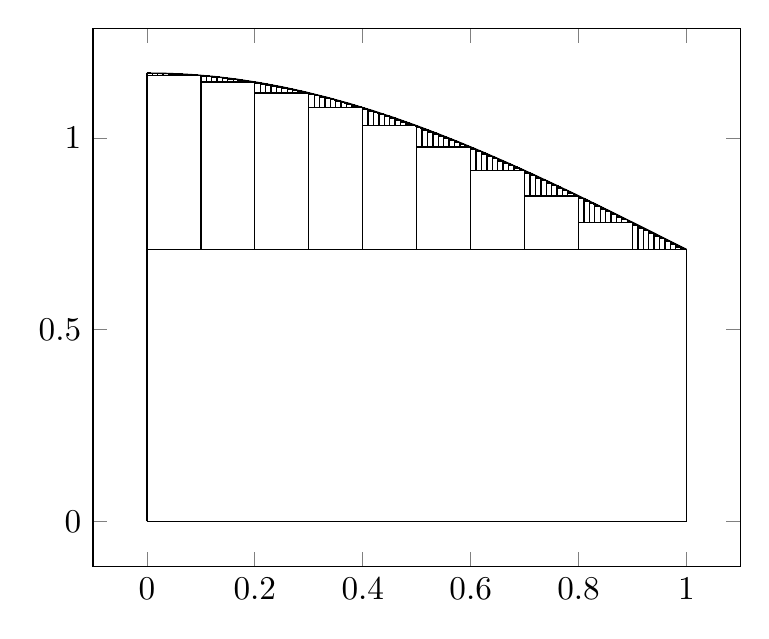
\begin{tikzpicture}[scale=1.2]
\begin{axis}
\addplot[draw=none] coordinates {(0,0)};
\addplot[domain=0:1] {e^(-x^2/2)/0.855624};
\draw (axis cs: 0, 0) -- (axis cs: 1, 0);
\draw (axis cs: 0, 0) -- (axis cs: 0, 0.7088752307384394);
\draw (axis cs: 1, 0) -- (axis cs: 1, 0.7088752307384394);
\draw (axis cs: 0, 0.7088752307384394) -- (axis cs: 1, 0.7088752307384394);
\draw (axis cs: 0, 0.7088752307384394) -- (axis cs: 0, 1.1629085663964824);
\draw (axis cs: 1/10, 0.7088752307384394) -- (axis cs: 1/10, 1.1629085663964824);
\draw (axis cs: 0, 1.1629085663964824) -- (axis cs: 1/10, 1.1629085663964824);
\draw (axis cs: 1/10, 0.7088752307384394) -- (axis cs: 1/10, 1.145595113479829);
\draw (axis cs: 1/5, 0.7088752307384394) -- (axis cs: 1/5, 1.145595113479829);
\draw (axis cs: 1/10, 1.145595113479829) -- (axis cs: 1/5, 1.145595113479829);
\draw (axis cs: 1/5, 0.7088752307384394) -- (axis cs: 1/5, 1.1173102694608443);
\draw (axis cs: 3/10, 0.7088752307384394) -- (axis cs: 3/10, 1.1173102694608443);
\draw (axis cs: 1/5, 1.1173102694608443) -- (axis cs: 3/10, 1.1173102694608443);
\draw (axis cs: 3/10, 0.7088752307384394) -- (axis cs: 3/10, 1.07888084786895);
\draw (axis cs: 2/5, 0.7088752307384394) -- (axis cs: 2/5, 1.07888084786895);
\draw (axis cs: 3/10, 1.07888084786895) -- (axis cs: 2/5, 1.07888084786895);
\draw (axis cs: 2/5, 0.7088752307384394) -- (axis cs: 2/5, 1.0314073740252947);
\draw (axis cs: 1/2, 0.7088752307384394) -- (axis cs: 1/2, 1.0314073740252947);
\draw (axis cs: 2/5, 1.0314073740252947) -- (axis cs: 1/2, 1.0314073740252947);
\draw (axis cs: 1/2, 0.7088752307384394) -- (axis cs: 1/2, 0.9762117610727802);
\draw (axis cs: 3/5, 0.7088752307384394) -- (axis cs: 3/5, 0.9762117610727802);
\draw (axis cs: 1/2, 0.9762117610727802) -- (axis cs: 3/5, 0.9762117610727802);
\draw (axis cs: 3/5, 0.7088752307384394) -- (axis cs: 3/5, 0.9147762786848253);
\draw (axis cs: 7/10, 0.7088752307384394) -- (axis cs: 7/10, 0.9147762786848253);
\draw (axis cs: 3/5, 0.9147762786848253) -- (axis cs: 7/10, 0.9147762786848253);
\draw (axis cs: 7/10, 0.7088752307384394) -- (axis cs: 7/10, 0.848677734546616);
\draw (axis cs: 4/5, 0.7088752307384394) -- (axis cs: 4/5, 0.848677734546616);
\draw (axis cs: 7/10, 0.848677734546616) -- (axis cs: 4/5, 0.848677734546616);
\draw (axis cs: 4/5, 0.7088752307384394) -- (axis cs: 4/5, 0.779520924795812);
\draw (axis cs: 9/10, 0.7088752307384394) -- (axis cs: 9/10, 0.779520924795812);
\draw (axis cs: 4/5, 0.779520924795812) -- (axis cs: 9/10, 0.779520924795812);
\draw (axis cs: 9/10, 0.7088752307384394) -- (axis cs: 9/10, 0.7088752309073);
\draw (axis cs: 1, 0.7088752307384394) -- (axis cs: 1, 0.7088752309073);
\draw (axis cs: 9/10, 0.7088752309073) -- (axis cs: 1, 0.7088752309073);
\draw (axis cs: 0, 1.1629085663964824) -- (axis cs: 0, 1.1686792343954033);
\draw (axis cs: 1/100, 1.1629085663964824) -- (axis cs: 1/100, 1.1686792343954033);
\draw (axis cs: 0, 1.1686792343954033) -- (axis cs: 1/100, 1.1686792343954033);
\draw (axis cs: 1/100, 1.1629085663964824) -- (axis cs: 1/100, 1.1685039456581519);
\draw (axis cs: 1/50, 1.1629085663964824) -- (axis cs: 1/50, 1.1685039456581519);
\draw (axis cs: 1/100, 1.1685039456581519) -- (axis cs: 1/50, 1.1685039456581519);
\draw (axis cs: 1/50, 1.1629085663964824) -- (axis cs: 1/50, 1.1682118561849484);
\draw (axis cs: 3/100, 1.1629085663964824) -- (axis cs: 3/100, 1.1682118561849484);
\draw (axis cs: 1/50, 1.1682118561849484) -- (axis cs: 3/100, 1.1682118561849484);
\draw (axis cs: 3/100, 1.1629085663964824) -- (axis cs: 3/100, 1.1678030535823951);
\draw (axis cs: 1/25, 1.1629085663964824) -- (axis cs: 1/25, 1.1678030535823951);
\draw (axis cs: 3/100, 1.1678030535823951) -- (axis cs: 1/25, 1.1678030535823951);
\draw (axis cs: 1/25, 1.1629085663964824) -- (axis cs: 1/25, 1.1672776604315254);
\draw (axis cs: 1/20, 1.1629085663964824) -- (axis cs: 1/20, 1.1672776604315254);
\draw (axis cs: 1/25, 1.1672776604315254) -- (axis cs: 1/20, 1.1672776604315254);
\draw (axis cs: 1/20, 1.1629085663964824) -- (axis cs: 1/20, 1.1666358342370182);
\draw (axis cs: 3/50, 1.1629085663964824) -- (axis cs: 3/50, 1.1666358342370182);
\draw (axis cs: 1/20, 1.1666358342370182) -- (axis cs: 3/50, 1.1666358342370182);
\draw (axis cs: 3/50, 1.1629085663964824) -- (axis cs: 3/50, 1.165877767349838);
\draw (axis cs: 7/100, 1.1629085663964824) -- (axis cs: 7/100, 1.165877767349838);
\draw (axis cs: 3/50, 1.165877767349838) -- (axis cs: 7/100, 1.165877767349838);
\draw (axis cs: 7/100, 1.1629085663964824) -- (axis cs: 7/100, 1.165003686847232);
\draw (axis cs: 2/25, 1.1629085663964824) -- (axis cs: 2/25, 1.165003686847232);
\draw (axis cs: 7/100, 1.165003686847232) -- (axis cs: 2/25, 1.165003686847232);
\draw (axis cs: 2/25, 1.1629085663964824) -- (axis cs: 2/25, 1.1640138544527399);
\draw (axis cs: 9/100, 1.1629085663964824) -- (axis cs: 9/100, 1.1640138544527399);
\draw (axis cs: 2/25, 1.1640138544527399) -- (axis cs: 9/100, 1.1640138544527399);
\draw (axis cs: 9/100, 1.1629085663964824) -- (axis cs: 9/100, 1.1629085663864607);
\draw (axis cs: 1/10, 1.1629085663964824) -- (axis cs: 1/10, 1.1629085663864607);
\draw (axis cs: 9/100, 1.1629085663864607) -- (axis cs: 1/10, 1.1629085663864607);
\draw (axis cs: 1/10, 1.145595113479829) -- (axis cs: 1/10, 1.1616881532210517);
\draw (axis cs: 11/100, 1.145595113479829) -- (axis cs: 11/100, 1.1616881532210517);
\draw (axis cs: 1/10, 1.1616881532210517) -- (axis cs: 11/100, 1.1616881532210517);
\draw (axis cs: 11/100, 1.145595113479829) -- (axis cs: 11/100, 1.1603529797348882);
\draw (axis cs: 3/25, 1.145595113479829) -- (axis cs: 3/25, 1.1603529797348882);
\draw (axis cs: 11/100, 1.1603529797348882) -- (axis cs: 3/25, 1.1603529797348882);
\draw (axis cs: 3/25, 1.145595113479829) -- (axis cs: 3/25, 1.158903444661192);
\draw (axis cs: 13/100, 1.145595113479829) -- (axis cs: 13/100, 1.158903444661192);
\draw (axis cs: 3/25, 1.158903444661192) -- (axis cs: 13/100, 1.158903444661192);
\draw (axis cs: 13/100, 1.145595113479829) -- (axis cs: 13/100, 1.1573399805893678);
\draw (axis cs: 7/50, 1.145595113479829) -- (axis cs: 7/50, 1.1573399805893678);
\draw (axis cs: 13/100, 1.1573399805893678) -- (axis cs: 7/50, 1.1573399805893678);
\draw (axis cs: 7/50, 1.145595113479829) -- (axis cs: 7/50, 1.155663053684396);
\draw (axis cs: 3/20, 1.145595113479829) -- (axis cs: 3/20, 1.155663053684396);
\draw (axis cs: 7/50, 1.155663053684396) -- (axis cs: 3/20, 1.155663053684396);
\draw (axis cs: 3/20, 1.145595113479829) -- (axis cs: 3/20, 1.1538731634752808);
\draw (axis cs: 4/25, 1.145595113479829) -- (axis cs: 4/25, 1.1538731634752808);
\draw (axis cs: 3/20, 1.1538731634752808) -- (axis cs: 4/25, 1.1538731634752808);
\draw (axis cs: 4/25, 1.145595113479829) -- (axis cs: 4/25, 1.1519708426024562);
\draw (axis cs: 17/100, 1.145595113479829) -- (axis cs: 17/100, 1.1519708426024562);
\draw (axis cs: 4/25, 1.1519708426024562) -- (axis cs: 17/100, 1.1519708426024562);
\draw (axis cs: 17/100, 1.145595113479829) -- (axis cs: 17/100, 1.1499566565550998);
\draw (axis cs: 9/50, 1.145595113479829) -- (axis cs: 9/50, 1.1499566565550998);
\draw (axis cs: 17/100, 1.1499566565550998) -- (axis cs: 9/50, 1.1499566565550998);
\draw (axis cs: 9/50, 1.145595113479829) -- (axis cs: 9/50, 1.1478312034346032);
\draw (axis cs: 19/100, 1.145595113479829) -- (axis cs: 19/100, 1.1478312034346032);
\draw (axis cs: 9/50, 1.1478312034346032) -- (axis cs: 19/100, 1.1478312034346032);
\draw (axis cs: 19/100, 1.145595113479829) -- (axis cs: 19/100, 1.14559511348866);
\draw (axis cs: 1/5, 1.145595113479829) -- (axis cs: 1/5, 1.14559511348866);
\draw (axis cs: 19/100, 1.14559511348866) -- (axis cs: 1/5, 1.14559511348866);
\draw (axis cs: 1/5, 1.1173102694608443) -- (axis cs: 1/5, 1.1432490490481584);
\draw (axis cs: 21/100, 1.1173102694608443) -- (axis cs: 21/100, 1.1432490490481584);
\draw (axis cs: 1/5, 1.1432490490481584) -- (axis cs: 21/100, 1.1432490490481584);
\draw (axis cs: 21/100, 1.1173102694608443) -- (axis cs: 21/100, 1.1407937040388867);
\draw (axis cs: 11/50, 1.1173102694608443) -- (axis cs: 11/50, 1.1407937040388867);
\draw (axis cs: 21/100, 1.1407937040388867) -- (axis cs: 11/50, 1.1407937040388867);
\draw (axis cs: 11/50, 1.1173102694608443) -- (axis cs: 11/50, 1.1382298036788177);
\draw (axis cs: 23/100, 1.1173102694608443) -- (axis cs: 23/100, 1.1382298036788177);
\draw (axis cs: 11/50, 1.1382298036788177) -- (axis cs: 23/100, 1.1382298036788177);
\draw (axis cs: 23/100, 1.1173102694608443) -- (axis cs: 23/100, 1.1355581041190577);
\draw (axis cs: 6/25, 1.1173102694608443) -- (axis cs: 6/25, 1.1355581041190577);
\draw (axis cs: 23/100, 1.1355581041190577) -- (axis cs: 6/25, 1.1355581041190577);
\draw (axis cs: 6/25, 1.1173102694608443) -- (axis cs: 6/25, 1.132779392077676);
\draw (axis cs: 1/4, 1.1173102694608443) -- (axis cs: 1/4, 1.132779392077676);
\draw (axis cs: 6/25, 1.132779392077676) -- (axis cs: 1/4, 1.132779392077676);
\draw (axis cs: 1/4, 1.1173102694608443) -- (axis cs: 1/4, 1.1298944844496572);
\draw (axis cs: 13/50, 1.1173102694608443) -- (axis cs: 13/50, 1.1298944844496572);
\draw (axis cs: 1/4, 1.1298944844496572) -- (axis cs: 13/50, 1.1298944844496572);
\draw (axis cs: 13/50, 1.1173102694608443) -- (axis cs: 13/50, 1.1269042279067734);
\draw (axis cs: 27/100, 1.1173102694608443) -- (axis cs: 27/100, 1.1269042279067734);
\draw (axis cs: 13/50, 1.1269042279067734) -- (axis cs: 27/100, 1.1269042279067734);
\draw (axis cs: 27/100, 1.1173102694608443) -- (axis cs: 27/100, 1.1238094984841474);
\draw (axis cs: 7/25, 1.1173102694608443) -- (axis cs: 7/25, 1.1238094984841474);
\draw (axis cs: 27/100, 1.1238094984841474) -- (axis cs: 7/25, 1.1238094984841474);
\draw (axis cs: 7/25, 1.1173102694608443) -- (axis cs: 7/25, 1.120611201152623);
\draw (axis cs: 29/100, 1.1173102694608443) -- (axis cs: 29/100, 1.120611201152623);
\draw (axis cs: 7/25, 1.120611201152623) -- (axis cs: 29/100, 1.120611201152623);
\draw (axis cs: 29/100, 1.1173102694608443) -- (axis cs: 29/100, 1.1173102693778385);
\draw (axis cs: 3/10, 1.1173102694608443) -- (axis cs: 3/10, 1.1173102693778385);
\draw (axis cs: 29/100, 1.1173102693778385) -- (axis cs: 3/10, 1.1173102693778385);
\draw (axis cs: 3/10, 1.07888084786895) -- (axis cs: 3/10, 1.1139076647768087);
\draw (axis cs: 31/100, 1.07888084786895) -- (axis cs: 31/100, 1.1139076647768087);
\draw (axis cs: 3/10, 1.1139076647768087) -- (axis cs: 31/100, 1.1139076647768087);
\draw (axis cs: 31/100, 1.07888084786895) -- (axis cs: 31/100, 1.110404376216082);
\draw (axis cs: 8/25, 1.07888084786895) -- (axis cs: 8/25, 1.110404376216082);
\draw (axis cs: 31/100, 1.110404376216082) -- (axis cs: 8/25, 1.110404376216082);
\draw (axis cs: 8/25, 1.07888084786895) -- (axis cs: 8/25, 1.1068014199756553);
\draw (axis cs: 33/100, 1.07888084786895) -- (axis cs: 33/100, 1.1068014199756553);
\draw (axis cs: 8/25, 1.1068014199756553) -- (axis cs: 33/100, 1.1068014199756553);
\draw (axis cs: 33/100, 1.07888084786895) -- (axis cs: 33/100, 1.1030998388359048);
\draw (axis cs: 17/50, 1.07888084786895) -- (axis cs: 17/50, 1.1030998388359048);
\draw (axis cs: 33/100, 1.1030998388359048) -- (axis cs: 17/50, 1.1030998388359048);
\draw (axis cs: 17/50, 1.07888084786895) -- (axis cs: 17/50, 1.0993007016787717);
\draw (axis cs: 7/20, 1.07888084786895) -- (axis cs: 7/20, 1.0993007016787717);
\draw (axis cs: 17/50, 1.0993007016787717) -- (axis cs: 7/20, 1.0993007016787717);
\draw (axis cs: 7/20, 1.07888084786895) -- (axis cs: 7/20, 1.0954051029736647);
\draw (axis cs: 9/25, 1.07888084786895) -- (axis cs: 9/25, 1.0954051029736647);
\draw (axis cs: 7/20, 1.0954051029736647) -- (axis cs: 9/25, 1.0954051029736647);
\draw (axis cs: 9/25, 1.07888084786895) -- (axis cs: 9/25, 1.0914141622523388);
\draw (axis cs: 37/100, 1.07888084786895) -- (axis cs: 37/100, 1.0914141622523388);
\draw (axis cs: 9/25, 1.0914141622523388) -- (axis cs: 37/100, 1.0914141622523388);
\draw (axis cs: 37/100, 1.07888084786895) -- (axis cs: 37/100, 1.087329023573098);
\draw (axis cs: 19/50, 1.07888084786895) -- (axis cs: 19/50, 1.087329023573098);
\draw (axis cs: 37/100, 1.087329023573098) -- (axis cs: 19/50, 1.087329023573098);
\draw (axis cs: 19/50, 1.07888084786895) -- (axis cs: 19/50, 1.0831508549713462);
\draw (axis cs: 39/100, 1.07888084786895) -- (axis cs: 39/100, 1.0831508549713462);
\draw (axis cs: 19/50, 1.0831508549713462) -- (axis cs: 39/100, 1.0831508549713462);
\draw (axis cs: 39/100, 1.07888084786895) -- (axis cs: 39/100, 1.0788808479124965);
\draw (axis cs: 2/5, 1.07888084786895) -- (axis cs: 2/5, 1.0788808479124965);
\draw (axis cs: 39/100, 1.0788808479124965) -- (axis cs: 2/5, 1.0788808479124965);
\draw (axis cs: 2/5, 1.0314073740252947) -- (axis cs: 2/5, 1.0745202167192769);
\draw (axis cs: 41/100, 1.0314073740252947) -- (axis cs: 41/100, 1.0745202167192769);
\draw (axis cs: 2/5, 1.0745202167192769) -- (axis cs: 41/100, 1.0745202167192769);
\draw (axis cs: 41/100, 1.0314073740252947) -- (axis cs: 41/100, 1.0700701979974419);
\draw (axis cs: 21/50, 1.0314073740252947) -- (axis cs: 21/50, 1.0700701979974419);
\draw (axis cs: 41/100, 1.0700701979974419) -- (axis cs: 21/50, 1.0700701979974419);
\draw (axis cs: 21/50, 1.0314073740252947) -- (axis cs: 21/50, 1.0655320500529688);
\draw (axis cs: 43/100, 1.0314073740252947) -- (axis cs: 43/100, 1.0655320500529688);
\draw (axis cs: 21/50, 1.0655320500529688) -- (axis cs: 43/100, 1.0655320500529688);
\draw (axis cs: 43/100, 1.0314073740252947) -- (axis cs: 43/100, 1.06090705229995);
\draw (axis cs: 11/25, 1.0314073740252947) -- (axis cs: 11/25, 1.06090705229995);
\draw (axis cs: 43/100, 1.06090705229995) -- (axis cs: 11/25, 1.06090705229995);
\draw (axis cs: 11/25, 1.0314073740252947) -- (axis cs: 11/25, 1.0561965046604347);
\draw (axis cs: 9/20, 1.0314073740252947) -- (axis cs: 9/20, 1.0561965046604347);
\draw (axis cs: 11/25, 1.0561965046604347) -- (axis cs: 9/20, 1.0561965046604347);
\draw (axis cs: 9/20, 1.0314073740252947) -- (axis cs: 9/20, 1.051401726956616);
\draw (axis cs: 23/50, 1.0314073740252947) -- (axis cs: 23/50, 1.051401726956616);
\draw (axis cs: 9/20, 1.051401726956616) -- (axis cs: 23/50, 1.051401726956616);
\draw (axis cs: 23/50, 1.0314073740252947) -- (axis cs: 23/50, 1.0465240582957578);
\draw (axis cs: 47/100, 1.0314073740252947) -- (axis cs: 47/100, 1.0465240582957578);
\draw (axis cs: 23/50, 1.0465240582957578) -- (axis cs: 47/100, 1.0465240582957578);
\draw (axis cs: 47/100, 1.0314073740252947) -- (axis cs: 47/100, 1.0415648564482645);
\draw (axis cs: 12/25, 1.0314073740252947) -- (axis cs: 12/25, 1.0415648564482645);
\draw (axis cs: 47/100, 1.0415648564482645) -- (axis cs: 12/25, 1.0415648564482645);
\draw (axis cs: 12/25, 1.0314073740252947) -- (axis cs: 12/25, 1.0365254972192939);
\draw (axis cs: 49/100, 1.0314073740252947) -- (axis cs: 49/100, 1.0365254972192939);
\draw (axis cs: 12/25, 1.0365254972192939) -- (axis cs: 49/100, 1.0365254972192939);
\draw (axis cs: 49/100, 1.0314073740252947) -- (axis cs: 49/100, 1.031407373814324);
\draw (axis cs: 1/2, 1.0314073740252947) -- (axis cs: 1/2, 1.031407373814324);
\draw (axis cs: 49/100, 1.031407373814324) -- (axis cs: 1/2, 1.031407373814324);
\draw (axis cs: 1/2, 0.9762117610727802) -- (axis cs: 1/2, 1.0262118964712261);
\draw (axis cs: 51/100, 0.9762117610727802) -- (axis cs: 51/100, 1.0262118964712261);
\draw (axis cs: 1/2, 1.0262118964712261) -- (axis cs: 51/100, 1.0262118964712261);
\draw (axis cs: 51/100, 0.9762117610727802) -- (axis cs: 51/100, 1.0209404907355755);
\draw (axis cs: 13/25, 0.9762117610727802) -- (axis cs: 13/25, 1.0209404907355755);
\draw (axis cs: 51/100, 1.0209404907355755) -- (axis cs: 13/25, 1.0209404907355755);
\draw (axis cs: 13/25, 0.9762117610727802) -- (axis cs: 13/25, 1.0155945984158463);
\draw (axis cs: 53/100, 0.9762117610727802) -- (axis cs: 53/100, 1.0155945984158463);
\draw (axis cs: 13/25, 1.0155945984158463) -- (axis cs: 53/100, 1.0155945984158463);
\draw (axis cs: 53/100, 0.9762117610727802) -- (axis cs: 53/100, 1.010175675867788);
\draw (axis cs: 27/50, 0.9762117610727802) -- (axis cs: 27/50, 1.010175675867788);
\draw (axis cs: 53/100, 1.010175675867788) -- (axis cs: 27/50, 1.010175675867788);
\draw (axis cs: 27/50, 0.9762117610727802) -- (axis cs: 27/50, 1.0046851935989134);
\draw (axis cs: 11/20, 0.9762117610727802) -- (axis cs: 11/20, 1.0046851935989134);
\draw (axis cs: 27/50, 1.0046851935989134) -- (axis cs: 11/20, 1.0046851935989134);
\draw (axis cs: 11/20, 0.9762117610727802) -- (axis cs: 11/20, 0.9991246356064033);
\draw (axis cs: 14/25, 0.9762117610727802) -- (axis cs: 14/25, 0.9991246356064033);
\draw (axis cs: 11/20, 0.9991246356064033) -- (axis cs: 14/25, 0.9991246356064033);
\draw (axis cs: 14/25, 0.9762117610727802) -- (axis cs: 14/25, 0.9934954987118504);
\draw (axis cs: 57/100, 0.9762117610727802) -- (axis cs: 57/100, 0.9934954987118504);
\draw (axis cs: 14/25, 0.9934954987118504) -- (axis cs: 57/100, 0.9934954987118504);
\draw (axis cs: 57/100, 0.9762117610727802) -- (axis cs: 57/100, 0.9877992918932575);
\draw (axis cs: 29/50, 0.9762117610727802) -- (axis cs: 29/50, 0.9877992918932575);
\draw (axis cs: 57/100, 0.9877992918932575) -- (axis cs: 29/50, 0.9877992918932575);
\draw (axis cs: 29/50, 0.9762117610727802) -- (axis cs: 29/50, 0.9820375356147064);
\draw (axis cs: 59/100, 0.9762117610727802) -- (axis cs: 59/100, 0.9820375356147064);
\draw (axis cs: 29/50, 0.9820375356147064) -- (axis cs: 59/100, 0.9820375356147064);
\draw (axis cs: 59/100, 0.9762117610727802) -- (axis cs: 59/100, 0.9762117611541081);
\draw (axis cs: 3/5, 0.9762117610727802) -- (axis cs: 3/5, 0.9762117611541081);
\draw (axis cs: 59/100, 0.9762117611541081) -- (axis cs: 3/5, 0.9762117611541081);
\draw (axis cs: 3/5, 0.9147762786848253) -- (axis cs: 3/5, 0.9703235099294532);
\draw (axis cs: 61/100, 0.9147762786848253) -- (axis cs: 61/100, 0.9703235099294532);
\draw (axis cs: 3/5, 0.9703235099294532) -- (axis cs: 61/100, 0.9703235099294532);
\draw (axis cs: 61/100, 0.9147762786848253) -- (axis cs: 61/100, 0.9643743328239671);
\draw (axis cs: 31/50, 0.9147762786848253) -- (axis cs: 31/50, 0.9643743328239671);
\draw (axis cs: 61/100, 0.9643743328239671) -- (axis cs: 31/50, 0.9643743328239671);
\draw (axis cs: 31/50, 0.9147762786848253) -- (axis cs: 31/50, 0.9583657895072194);
\draw (axis cs: 63/100, 0.9147762786848253) -- (axis cs: 63/100, 0.9583657895072194);
\draw (axis cs: 31/50, 0.9583657895072194) -- (axis cs: 63/100, 0.9583657895072194);
\draw (axis cs: 63/100, 0.9147762786848253) -- (axis cs: 63/100, 0.9522994477666723);
\draw (axis cs: 16/25, 0.9147762786848253) -- (axis cs: 16/25, 0.9522994477666723);
\draw (axis cs: 63/100, 0.9522994477666723) -- (axis cs: 16/25, 0.9522994477666723);
\draw (axis cs: 16/25, 0.9147762786848253) -- (axis cs: 16/25, 0.9461768828300766);
\draw (axis cs: 13/20, 0.9147762786848253) -- (axis cs: 13/20, 0.9461768828300766);
\draw (axis cs: 16/25, 0.9461768828300766) -- (axis cs: 13/20, 0.9461768828300766);
\draw (axis cs: 13/20, 0.9147762786848253) -- (axis cs: 13/20, 0.939999676685661);
\draw (axis cs: 33/50, 0.9147762786848253) -- (axis cs: 33/50, 0.939999676685661);
\draw (axis cs: 13/20, 0.939999676685661) -- (axis cs: 33/50, 0.939999676685661);
\draw (axis cs: 33/50, 0.9147762786848253) -- (axis cs: 33/50, 0.9337694174105843);
\draw (axis cs: 67/100, 0.9147762786848253) -- (axis cs: 67/100, 0.9337694174105843);
\draw (axis cs: 33/50, 0.9337694174105843) -- (axis cs: 67/100, 0.9337694174105843);
\draw (axis cs: 67/100, 0.9147762786848253) -- (axis cs: 67/100, 0.9274876984980764);
\draw (axis cs: 17/25, 0.9147762786848253) -- (axis cs: 17/25, 0.9274876984980764);
\draw (axis cs: 67/100, 0.9274876984980764) -- (axis cs: 17/25, 0.9274876984980764);
\draw (axis cs: 17/25, 0.9147762786848253) -- (axis cs: 17/25, 0.9211561181863079);
\draw (axis cs: 69/100, 0.9147762786848253) -- (axis cs: 69/100, 0.9211561181863079);
\draw (axis cs: 17/25, 0.9211561181863079) -- (axis cs: 69/100, 0.9211561181863079);
\draw (axis cs: 69/100, 0.9147762786848253) -- (axis cs: 69/100, 0.9147762787893747);
\draw (axis cs: 7/10, 0.9147762786848253) -- (axis cs: 7/10, 0.9147762787893747);
\draw (axis cs: 69/100, 0.9147762787893747) -- (axis cs: 7/10, 0.9147762787893747);
\draw (axis cs: 7/10, 0.848677734546616) -- (axis cs: 7/10, 0.9083497860307876);
\draw (axis cs: 71/100, 0.848677734546616) -- (axis cs: 71/100, 0.9083497860307876);
\draw (axis cs: 7/10, 0.9083497860307876) -- (axis cs: 71/100, 0.9083497860307876);
\draw (axis cs: 71/100, 0.848677734546616) -- (axis cs: 71/100, 0.9018782483798445);
\draw (axis cs: 18/25, 0.848677734546616) -- (axis cs: 18/25, 0.9018782483798445);
\draw (axis cs: 71/100, 0.9018782483798445) -- (axis cs: 18/25, 0.9018782483798445);
\draw (axis cs: 18/25, 0.848677734546616) -- (axis cs: 18/25, 0.8953632763912646);
\draw (axis cs: 73/100, 0.848677734546616) -- (axis cs: 73/100, 0.8953632763912646);
\draw (axis cs: 18/25, 0.8953632763912646) -- (axis cs: 73/100, 0.8953632763912646);
\draw (axis cs: 73/100, 0.848677734546616) -- (axis cs: 73/100, 0.8888064820484545);
\draw (axis cs: 37/50, 0.848677734546616) -- (axis cs: 37/50, 0.8888064820484545);
\draw (axis cs: 73/100, 0.8888064820484545) -- (axis cs: 37/50, 0.8888064820484545);
\draw (axis cs: 37/50, 0.848677734546616) -- (axis cs: 37/50, 0.8822094781107758);
\draw (axis cs: 3/4, 0.848677734546616) -- (axis cs: 3/4, 0.8822094781107758);
\draw (axis cs: 37/50, 0.8822094781107758) -- (axis cs: 3/4, 0.8822094781107758);
\draw (axis cs: 3/4, 0.848677734546616) -- (axis cs: 3/4, 0.8755738774651708);
\draw (axis cs: 19/25, 0.848677734546616) -- (axis cs: 19/25, 0.8755738774651708);
\draw (axis cs: 3/4, 0.8755738774651708) -- (axis cs: 19/25, 0.8755738774651708);
\draw (axis cs: 19/25, 0.848677734546616) -- (axis cs: 19/25, 0.868901292482507);
\draw (axis cs: 77/100, 0.848677734546616) -- (axis cs: 77/100, 0.868901292482507);
\draw (axis cs: 19/25, 0.868901292482507) -- (axis cs: 77/100, 0.868901292482507);
\draw (axis cs: 77/100, 0.848677734546616) -- (axis cs: 77/100, 0.8621933343789866);
\draw (axis cs: 39/50, 0.848677734546616) -- (axis cs: 39/50, 0.8621933343789866);
\draw (axis cs: 77/100, 0.8621933343789866) -- (axis cs: 39/50, 0.8621933343789866);
\draw (axis cs: 39/50, 0.848677734546616) -- (axis cs: 39/50, 0.8554516125829663);
\draw (axis cs: 79/100, 0.848677734546616) -- (axis cs: 79/100, 0.8554516125829663);
\draw (axis cs: 39/50, 0.8554516125829663) -- (axis cs: 79/100, 0.8554516125829663);
\draw (axis cs: 79/100, 0.848677734546616) -- (axis cs: 79/100, 0.8486777341075245);
\draw (axis cs: 4/5, 0.848677734546616) -- (axis cs: 4/5, 0.8486777341075245);
\draw (axis cs: 79/100, 0.8486777341075245) -- (axis cs: 4/5, 0.8486777341075245);
\draw (axis cs: 4/5, 0.779520924795812) -- (axis cs: 4/5, 0.8418733029291042);
\draw (axis cs: 81/100, 0.779520924795812) -- (axis cs: 81/100, 0.8418733029291042);
\draw (axis cs: 4/5, 0.8418733029291042) -- (axis cs: 81/100, 0.8418733029291042);
\draw (axis cs: 81/100, 0.779520924795812) -- (axis cs: 81/100, 0.8350399193725604);
\draw (axis cs: 41/50, 0.779520924795812) -- (axis cs: 41/50, 0.8350399193725604);
\draw (axis cs: 81/100, 0.8350399193725604) -- (axis cs: 41/50, 0.8350399193725604);
\draw (axis cs: 41/50, 0.779520924795812) -- (axis cs: 41/50, 0.8281791800803281);
\draw (axis cs: 83/100, 0.779520924795812) -- (axis cs: 83/100, 0.8281791800803281);
\draw (axis cs: 41/50, 0.8281791800803281) -- (axis cs: 83/100, 0.8281791800803281);
\draw (axis cs: 83/100, 0.779520924795812) -- (axis cs: 83/100, 0.8212926751105863);
\draw (axis cs: 21/25, 0.779520924795812) -- (axis cs: 21/25, 0.8212926751105863);
\draw (axis cs: 83/100, 0.8212926751105863) -- (axis cs: 21/25, 0.8212926751105863);
\draw (axis cs: 21/25, 0.779520924795812) -- (axis cs: 21/25, 0.8143819907807417);
\draw (axis cs: 17/20, 0.779520924795812) -- (axis cs: 17/20, 0.8143819907807417);
\draw (axis cs: 21/25, 0.8143819907807417) -- (axis cs: 17/20, 0.8143819907807417);
\draw (axis cs: 17/20, 0.779520924795812) -- (axis cs: 17/20, 0.807448706798706);
\draw (axis cs: 43/50, 0.779520924795812) -- (axis cs: 43/50, 0.807448706798706);
\draw (axis cs: 17/20, 0.807448706798706) -- (axis cs: 43/50, 0.807448706798706);
\draw (axis cs: 43/50, 0.779520924795812) -- (axis cs: 43/50, 0.8004943962528822);
\draw (axis cs: 87/100, 0.779520924795812) -- (axis cs: 87/100, 0.8004943962528822);
\draw (axis cs: 43/50, 0.8004943962528822) -- (axis cs: 87/100, 0.8004943962528822);
\draw (axis cs: 87/100, 0.779520924795812) -- (axis cs: 87/100, 0.793520625042011);
\draw (axis cs: 22/25, 0.779520924795812) -- (axis cs: 22/25, 0.793520625042011);
\draw (axis cs: 87/100, 0.793520625042011) -- (axis cs: 22/25, 0.793520625042011);
\draw (axis cs: 22/25, 0.779520924795812) -- (axis cs: 22/25, 0.7865289513134806);
\draw (axis cs: 89/100, 0.779520924795812) -- (axis cs: 89/100, 0.7865289513134806);
\draw (axis cs: 22/25, 0.7865289513134806) -- (axis cs: 89/100, 0.7865289513134806);
\draw (axis cs: 89/100, 0.779520924795812) -- (axis cs: 89/100, 0.779520924910358);
\draw (axis cs: 9/10, 0.779520924795812) -- (axis cs: 9/10, 0.779520924910358);
\draw (axis cs: 89/100, 0.779520924910358) -- (axis cs: 9/10, 0.779520924910358);
\draw (axis cs: 9/10, 0.7088752309073) -- (axis cs: 9/10, 0.772498086827401);
\draw (axis cs: 91/100, 0.7088752309073) -- (axis cs: 91/100, 0.772498086827401);
\draw (axis cs: 9/10, 0.772498086827401) -- (axis cs: 91/100, 0.772498086827401);
\draw (axis cs: 91/100, 0.7088752309073) -- (axis cs: 91/100, 0.7654619686762921);
\draw (axis cs: 23/25, 0.7088752309073) -- (axis cs: 23/25, 0.7654619686762921);
\draw (axis cs: 91/100, 0.7654619686762921) -- (axis cs: 23/25, 0.7654619686762921);
\draw (axis cs: 23/25, 0.7088752309073) -- (axis cs: 23/25, 0.7584140921603341);
\draw (axis cs: 93/100, 0.7088752309073) -- (axis cs: 93/100, 0.7584140921603341);
\draw (axis cs: 23/25, 0.7584140921603341) -- (axis cs: 93/100, 0.7584140921603341);
\draw (axis cs: 93/100, 0.7088752309073) -- (axis cs: 93/100, 0.7513559685588359);
\draw (axis cs: 47/50, 0.7088752309073) -- (axis cs: 47/50, 0.7513559685588359);
\draw (axis cs: 93/100, 0.7513559685588359) -- (axis cs: 47/50, 0.7513559685588359);
\draw (axis cs: 47/50, 0.7088752309073) -- (axis cs: 47/50, 0.7442890982214072);
\draw (axis cs: 19/20, 0.7088752309073) -- (axis cs: 19/20, 0.7442890982214072);
\draw (axis cs: 47/50, 0.7442890982214072) -- (axis cs: 19/20, 0.7442890982214072);
\draw (axis cs: 19/20, 0.7088752309073) -- (axis cs: 19/20, 0.7372149700723738);
\draw (axis cs: 24/25, 0.7088752309073) -- (axis cs: 24/25, 0.7372149700723738);
\draw (axis cs: 19/20, 0.7372149700723738) -- (axis cs: 24/25, 0.7372149700723738);
\draw (axis cs: 24/25, 0.7088752309073) -- (axis cs: 24/25, 0.7301350611255129);
\draw (axis cs: 97/100, 0.7088752309073) -- (axis cs: 97/100, 0.7301350611255129);
\draw (axis cs: 24/25, 0.7301350611255129) -- (axis cs: 97/100, 0.7301350611255129);
\draw (axis cs: 97/100, 0.7088752309073) -- (axis cs: 97/100, 0.7230508360093055);
\draw (axis cs: 49/50, 0.7088752309073) -- (axis cs: 49/50, 0.7230508360093055);
\draw (axis cs: 97/100, 0.7230508360093055) -- (axis cs: 49/50, 0.7230508360093055);
\draw (axis cs: 49/50, 0.7088752309073) -- (axis cs: 49/50, 0.7159637465028859);
\draw (axis cs: 99/100, 0.7088752309073) -- (axis cs: 99/100, 0.7159637465028859);
\draw (axis cs: 49/50, 0.7159637465028859) -- (axis cs: 99/100, 0.7159637465028859);
\draw (axis cs: 99/100, 0.7088752309073) -- (axis cs: 99/100, 0.7088752310828618);
\draw (axis cs: 1, 0.7088752309073) -- (axis cs: 1, 0.7088752310828618);
\draw (axis cs: 99/100, 0.7088752310828618) -- (axis cs: 1, 0.7088752310828618);
\draw (axis cs: 0, 1.1686792343954033) -- (axis cs: 0, 1.16873708544891);
\draw (axis cs: 1/1000, 1.1686792343954033) -- (axis cs: 1/1000, 1.16873708544891);
\draw (axis cs: 0, 1.16873708544891) -- (axis cs: 1/1000, 1.16873708544891);
\draw (axis cs: 1/1000, 1.1686792343954033) -- (axis cs: 1/1000, 1.1687353323446097);
\draw (axis cs: 1/500, 1.1686792343954033) -- (axis cs: 1/500, 1.1687353323446097);
\draw (axis cs: 1/1000, 1.1687353323446097) -- (axis cs: 1/500, 1.1687353323446097);
\draw (axis cs: 1/500, 1.1686792343954033) -- (axis cs: 1/500, 1.1687324105099877);
\draw (axis cs: 3/1000, 1.1686792343954033) -- (axis cs: 3/1000, 1.1687324105099877);
\draw (axis cs: 1/500, 1.1687324105099877) -- (axis cs: 3/1000, 1.1687324105099877);
\draw (axis cs: 3/1000, 1.1686792343954033) -- (axis cs: 3/1000, 1.1687283199537377);
\draw (axis cs: 1/250, 1.1686792343954033) -- (axis cs: 1/250, 1.1687283199537377);
\draw (axis cs: 3/1000, 1.1687283199537377) -- (axis cs: 1/250, 1.1687283199537377);
\draw (axis cs: 1/250, 1.1686792343954033) -- (axis cs: 1/250, 1.1687230606881593);
\draw (axis cs: 1/200, 1.1686792343954033) -- (axis cs: 1/200, 1.1687230606881593);
\draw (axis cs: 1/250, 1.1687230606881593) -- (axis cs: 1/200, 1.1687230606881593);
\draw (axis cs: 1/200, 1.1686792343954033) -- (axis cs: 1/200, 1.1687166327290237);
\draw (axis cs: 3/500, 1.1686792343954033) -- (axis cs: 3/500, 1.1687166327290237);
\draw (axis cs: 1/200, 1.1687166327290237) -- (axis cs: 3/500, 1.1687166327290237);
\draw (axis cs: 3/500, 1.1686792343954033) -- (axis cs: 3/500, 1.1687090360956192);
\draw (axis cs: 7/1000, 1.1686792343954033) -- (axis cs: 7/1000, 1.1687090360956192);
\draw (axis cs: 3/500, 1.1687090360956192) -- (axis cs: 7/1000, 1.1687090360956192);
\draw (axis cs: 7/1000, 1.1686792343954033) -- (axis cs: 7/1000, 1.1687002708107348);
\draw (axis cs: 1/125, 1.1686792343954033) -- (axis cs: 1/125, 1.1687002708107348);
\draw (axis cs: 7/1000, 1.1687002708107348) -- (axis cs: 1/125, 1.1687002708107348);
\draw (axis cs: 1/125, 1.1686792343954033) -- (axis cs: 1/125, 1.1686903369006665);
\draw (axis cs: 9/1000, 1.1686792343954033) -- (axis cs: 9/1000, 1.1686903369006665);
\draw (axis cs: 1/125, 1.1686903369006665) -- (axis cs: 9/1000, 1.1686903369006665);
\draw (axis cs: 9/1000, 1.1686792343954033) -- (axis cs: 9/1000, 1.1686792343954484);
\draw (axis cs: 1/100, 1.1686792343954033) -- (axis cs: 1/100, 1.1686792343954484);
\draw (axis cs: 9/1000, 1.1686792343954484) -- (axis cs: 1/100, 1.1686792343954484);
\draw (axis cs: 1/100, 1.1685039456581519) -- (axis cs: 1/100, 1.1686669633279563);
\draw (axis cs: 11/1000, 1.1685039456581519) -- (axis cs: 11/1000, 1.1686669633279563);
\draw (axis cs: 1/100, 1.1686669633279563) -- (axis cs: 11/1000, 1.1686669633279563);
\draw (axis cs: 11/1000, 1.1685039456581519) -- (axis cs: 11/1000, 1.1686535237352018);
\draw (axis cs: 3/250, 1.1685039456581519) -- (axis cs: 3/250, 1.1686535237352018);
\draw (axis cs: 11/1000, 1.1686535237352018) -- (axis cs: 3/250, 1.1686535237352018);
\draw (axis cs: 3/250, 1.1685039456581519) -- (axis cs: 3/250, 1.1686389156575014);
\draw (axis cs: 13/1000, 1.1685039456581519) -- (axis cs: 13/1000, 1.1686389156575014);
\draw (axis cs: 3/250, 1.1686389156575014) -- (axis cs: 13/1000, 1.1686389156575014);
\draw (axis cs: 13/1000, 1.1685039456581519) -- (axis cs: 13/1000, 1.1686231391386777);
\draw (axis cs: 7/500, 1.1685039456581519) -- (axis cs: 7/500, 1.1686231391386777);
\draw (axis cs: 13/1000, 1.1686231391386777) -- (axis cs: 7/500, 1.1686231391386777);
\draw (axis cs: 7/500, 1.1685039456581519) -- (axis cs: 7/500, 1.1686061942260435);
\draw (axis cs: 3/200, 1.1685039456581519) -- (axis cs: 3/200, 1.1686061942260435);
\draw (axis cs: 7/500, 1.1686061942260435) -- (axis cs: 3/200, 1.1686061942260435);
\draw (axis cs: 3/200, 1.1685039456581519) -- (axis cs: 3/200, 1.1685880809704374);
\draw (axis cs: 2/125, 1.1685039456581519) -- (axis cs: 2/125, 1.1685880809704374);
\draw (axis cs: 3/200, 1.1685880809704374) -- (axis cs: 2/125, 1.1685880809704374);
\draw (axis cs: 2/125, 1.1685039456581519) -- (axis cs: 2/125, 1.1685687994261984);
\draw (axis cs: 17/1000, 1.1685039456581519) -- (axis cs: 17/1000, 1.1685687994261984);
\draw (axis cs: 2/125, 1.1685687994261984) -- (axis cs: 17/1000, 1.1685687994261984);
\draw (axis cs: 17/1000, 1.1685039456581519) -- (axis cs: 17/1000, 1.168548349651166);
\draw (axis cs: 9/500, 1.1685039456581519) -- (axis cs: 9/500, 1.168548349651166);
\draw (axis cs: 17/1000, 1.168548349651166) -- (axis cs: 9/500, 1.168548349651166);
\draw (axis cs: 9/500, 1.1685039456581519) -- (axis cs: 9/500, 1.1685267317066834);
\draw (axis cs: 19/1000, 1.1685039456581519) -- (axis cs: 19/1000, 1.1685267317066834);
\draw (axis cs: 9/500, 1.1685267317066834) -- (axis cs: 19/1000, 1.1685267317066834);
\draw (axis cs: 19/1000, 1.1685039456581519) -- (axis cs: 19/1000, 1.1685039456575965);
\draw (axis cs: 1/50, 1.1685039456581519) -- (axis cs: 1/50, 1.1685039456575965);
\draw (axis cs: 19/1000, 1.1685039456575965) -- (axis cs: 1/50, 1.1685039456575965);
\draw (axis cs: 1/50, 1.1682118561849484) -- (axis cs: 1/50, 1.1684799915722552);
\draw (axis cs: 21/1000, 1.1682118561849484) -- (axis cs: 21/1000, 1.1684799915722552);
\draw (axis cs: 1/50, 1.1684799915722552) -- (axis cs: 21/1000, 1.1684799915722552);
\draw (axis cs: 21/1000, 1.1682118561849484) -- (axis cs: 21/1000, 1.1684548695233343);
\draw (axis cs: 11/500, 1.1682118561849484) -- (axis cs: 11/500, 1.1684548695233343);
\draw (axis cs: 21/1000, 1.1684548695233343) -- (axis cs: 11/500, 1.1684548695233343);
\draw (axis cs: 11/500, 1.1682118561849484) -- (axis cs: 11/500, 1.168428579584607);
\draw (axis cs: 23/1000, 1.1682118561849484) -- (axis cs: 23/1000, 1.168428579584607);
\draw (axis cs: 11/500, 1.168428579584607) -- (axis cs: 23/1000, 1.168428579584607);
\draw (axis cs: 23/1000, 1.1682118561849484) -- (axis cs: 23/1000, 1.168401121835691);
\draw (axis cs: 3/125, 1.1682118561849484) -- (axis cs: 3/125, 1.168401121835691);
\draw (axis cs: 23/1000, 1.168401121835691) -- (axis cs: 3/125, 1.168401121835691);
\draw (axis cs: 3/125, 1.1682118561849484) -- (axis cs: 3/125, 1.1683724963589435);
\draw (axis cs: 1/40, 1.1682118561849484) -- (axis cs: 1/40, 1.1683724963589435);
\draw (axis cs: 3/125, 1.1683724963589435) -- (axis cs: 1/40, 1.1683724963589435);
\draw (axis cs: 1/40, 1.1682118561849484) -- (axis cs: 1/40, 1.1683427032402243);
\draw (axis cs: 13/500, 1.1682118561849484) -- (axis cs: 13/500, 1.1683427032402243);
\draw (axis cs: 1/40, 1.1683427032402243) -- (axis cs: 13/500, 1.1683427032402243);
\draw (axis cs: 13/500, 1.1682118561849484) -- (axis cs: 13/500, 1.1683117425688934);
\draw (axis cs: 27/1000, 1.1682118561849484) -- (axis cs: 27/1000, 1.1683117425688934);
\draw (axis cs: 13/500, 1.1683117425688934) -- (axis cs: 27/1000, 1.1683117425688934);
\draw (axis cs: 27/1000, 1.1682118561849484) -- (axis cs: 27/1000, 1.1682796144378107);
\draw (axis cs: 7/250, 1.1682118561849484) -- (axis cs: 7/250, 1.1682796144378107);
\draw (axis cs: 27/1000, 1.1682796144378107) -- (axis cs: 7/250, 1.1682796144378107);
\draw (axis cs: 7/250, 1.1682118561849484) -- (axis cs: 7/250, 1.1682463189433363);
\draw (axis cs: 29/1000, 1.1682118561849484) -- (axis cs: 29/1000, 1.1682463189433363);
\draw (axis cs: 7/250, 1.1682463189433363) -- (axis cs: 29/1000, 1.1682463189433363);
\draw (axis cs: 29/1000, 1.1682118561849484) -- (axis cs: 29/1000, 1.1682118561853019);
\draw (axis cs: 3/100, 1.1682118561849484) -- (axis cs: 3/100, 1.1682118561853019);
\draw (axis cs: 29/1000, 1.1682118561853019) -- (axis cs: 3/100, 1.1682118561853019);
\draw (axis cs: 3/100, 1.1678030535823951) -- (axis cs: 3/100, 1.1681762262670843);
\draw (axis cs: 31/1000, 1.1678030535823951) -- (axis cs: 31/1000, 1.1681762262670843);
\draw (axis cs: 3/100, 1.1681762262670843) -- (axis cs: 31/1000, 1.1681762262670843);
\draw (axis cs: 31/1000, 1.1678030535823951) -- (axis cs: 31/1000, 1.168139429295547);
\draw (axis cs: 4/125, 1.1678030535823951) -- (axis cs: 4/125, 1.168139429295547);
\draw (axis cs: 31/1000, 1.168139429295547) -- (axis cs: 4/125, 1.168139429295547);
\draw (axis cs: 4/125, 1.1678030535823951) -- (axis cs: 4/125, 1.168101465381044);
\draw (axis cs: 33/1000, 1.1678030535823951) -- (axis cs: 33/1000, 1.168101465381044);
\draw (axis cs: 4/125, 1.168101465381044) -- (axis cs: 33/1000, 1.168101465381044);
\draw (axis cs: 33/1000, 1.1678030535823951) -- (axis cs: 33/1000, 1.1680623346374273);
\draw (axis cs: 17/500, 1.1678030535823951) -- (axis cs: 17/500, 1.1680623346374273);
\draw (axis cs: 33/1000, 1.1680623346374273) -- (axis cs: 17/500, 1.1680623346374273);
\draw (axis cs: 17/500, 1.1678030535823951) -- (axis cs: 17/500, 1.1680220371820451);
\draw (axis cs: 7/200, 1.1678030535823951) -- (axis cs: 7/200, 1.1680220371820451);
\draw (axis cs: 17/500, 1.1680220371820451) -- (axis cs: 7/200, 1.1680220371820451);
\draw (axis cs: 7/200, 1.1678030535823951) -- (axis cs: 7/200, 1.1679805731357418);
\draw (axis cs: 9/250, 1.1678030535823951) -- (axis cs: 9/250, 1.1679805731357418);
\draw (axis cs: 7/200, 1.1679805731357418) -- (axis cs: 9/250, 1.1679805731357418);
\draw (axis cs: 9/250, 1.1678030535823951) -- (axis cs: 9/250, 1.1679379426228567);
\draw (axis cs: 37/1000, 1.1678030535823951) -- (axis cs: 37/1000, 1.1679379426228567);
\draw (axis cs: 9/250, 1.1679379426228567) -- (axis cs: 37/1000, 1.1679379426228567);
\draw (axis cs: 37/1000, 1.1678030535823951) -- (axis cs: 37/1000, 1.167894145771225);
\draw (axis cs: 19/500, 1.1678030535823951) -- (axis cs: 19/500, 1.167894145771225);
\draw (axis cs: 37/1000, 1.167894145771225) -- (axis cs: 19/500, 1.167894145771225);
\draw (axis cs: 19/500, 1.1678030535823951) -- (axis cs: 19/500, 1.1678491827121757);
\draw (axis cs: 39/1000, 1.1678030535823951) -- (axis cs: 39/1000, 1.1678491827121757);
\draw (axis cs: 19/500, 1.1678491827121757) -- (axis cs: 39/1000, 1.1678491827121757);
\draw (axis cs: 39/1000, 1.1678030535823951) -- (axis cs: 39/1000, 1.1678030535805308);
\draw (axis cs: 1/25, 1.1678030535823951) -- (axis cs: 1/25, 1.1678030535805308);
\draw (axis cs: 39/1000, 1.1678030535805308) -- (axis cs: 1/25, 1.1678030535805308);
\draw (axis cs: 1/25, 1.1672776604315254) -- (axis cs: 1/25, 1.167755758514606);
\draw (axis cs: 41/1000, 1.1672776604315254) -- (axis cs: 41/1000, 1.167755758514606);
\draw (axis cs: 1/25, 1.167755758514606) -- (axis cs: 41/1000, 1.167755758514606);
\draw (axis cs: 41/1000, 1.1672776604315254) -- (axis cs: 41/1000, 1.1677072976587588);
\draw (axis cs: 21/500, 1.1672776604315254) -- (axis cs: 21/500, 1.1677072976587588);
\draw (axis cs: 41/1000, 1.1677072976587588) -- (axis cs: 21/500, 1.1677072976587588);
\draw (axis cs: 21/500, 1.1672776604315254) -- (axis cs: 21/500, 1.1676576711532989);
\draw (axis cs: 43/1000, 1.1672776604315254) -- (axis cs: 43/1000, 1.1676576711532989);
\draw (axis cs: 21/500, 1.1676576711532989) -- (axis cs: 43/1000, 1.1676576711532989);
\draw (axis cs: 43/1000, 1.1672776604315254) -- (axis cs: 43/1000, 1.1676068791494576);
\draw (axis cs: 11/250, 1.1672776604315254) -- (axis cs: 11/250, 1.1676068791494576);
\draw (axis cs: 43/1000, 1.1676068791494576) -- (axis cs: 11/250, 1.1676068791494576);
\draw (axis cs: 11/250, 1.1672776604315254) -- (axis cs: 11/250, 1.167554921799515);
\draw (axis cs: 9/200, 1.1672776604315254) -- (axis cs: 9/200, 1.167554921799515);
\draw (axis cs: 11/250, 1.167554921799515) -- (axis cs: 9/200, 1.167554921799515);
\draw (axis cs: 9/200, 1.1672776604315254) -- (axis cs: 9/200, 1.16750179925924);
\draw (axis cs: 23/500, 1.1672776604315254) -- (axis cs: 23/500, 1.16750179925924);
\draw (axis cs: 9/200, 1.16750179925924) -- (axis cs: 23/500, 1.16750179925924);
\draw (axis cs: 23/500, 1.1672776604315254) -- (axis cs: 23/500, 1.16744751168789);
\draw (axis cs: 47/1000, 1.1672776604315254) -- (axis cs: 47/1000, 1.16744751168789);
\draw (axis cs: 23/500, 1.16744751168789) -- (axis cs: 47/1000, 1.16744751168789);
\draw (axis cs: 47/1000, 1.1672776604315254) -- (axis cs: 47/1000, 1.1673920592482105);
\draw (axis cs: 6/125, 1.1672776604315254) -- (axis cs: 6/125, 1.1673920592482105);
\draw (axis cs: 47/1000, 1.1673920592482105) -- (axis cs: 6/125, 1.1673920592482105);
\draw (axis cs: 6/125, 1.1672776604315254) -- (axis cs: 6/125, 1.1673354421064337);
\draw (axis cs: 49/1000, 1.1672776604315254) -- (axis cs: 49/1000, 1.1673354421064337);
\draw (axis cs: 6/125, 1.1673354421064337) -- (axis cs: 49/1000, 1.1673354421064337);
\draw (axis cs: 49/1000, 1.1672776604315254) -- (axis cs: 49/1000, 1.1672776604322774);
\draw (axis cs: 1/20, 1.1672776604315254) -- (axis cs: 1/20, 1.1672776604322774);
\draw (axis cs: 49/1000, 1.1672776604322774) -- (axis cs: 1/20, 1.1672776604322774);
\draw (axis cs: 1/20, 1.1666358342370182) -- (axis cs: 1/20, 1.1672187143989454);
\draw (axis cs: 51/1000, 1.1666358342370182) -- (axis cs: 51/1000, 1.1672187143989454);
\draw (axis cs: 1/20, 1.1672187143989454) -- (axis cs: 51/1000, 1.1672187143989454);
\draw (axis cs: 51/1000, 1.1666358342370182) -- (axis cs: 51/1000, 1.167158604183125);
\draw (axis cs: 13/250, 1.1666358342370182) -- (axis cs: 13/250, 1.167158604183125);
\draw (axis cs: 51/1000, 1.167158604183125) -- (axis cs: 13/250, 1.167158604183125);
\draw (axis cs: 13/250, 1.1666358342370182) -- (axis cs: 13/250, 1.1670973299649874);
\draw (axis cs: 53/1000, 1.1666358342370182) -- (axis cs: 53/1000, 1.1670973299649874);
\draw (axis cs: 13/250, 1.1670973299649874) -- (axis cs: 53/1000, 1.1670973299649874);
\draw (axis cs: 53/1000, 1.1666358342370182) -- (axis cs: 53/1000, 1.1670348919281515);
\draw (axis cs: 27/500, 1.1666358342370182) -- (axis cs: 27/500, 1.1670348919281515);
\draw (axis cs: 53/1000, 1.1670348919281515) -- (axis cs: 27/500, 1.1670348919281515);
\draw (axis cs: 27/500, 1.1666358342370182) -- (axis cs: 27/500, 1.1669712902597575);
\draw (axis cs: 11/200, 1.1666358342370182) -- (axis cs: 11/200, 1.1669712902597575);
\draw (axis cs: 27/500, 1.1669712902597575) -- (axis cs: 11/200, 1.1669712902597575);
\draw (axis cs: 11/200, 1.1666358342370182) -- (axis cs: 11/200, 1.166906525150449);
\draw (axis cs: 7/125, 1.1666358342370182) -- (axis cs: 7/125, 1.166906525150449);
\draw (axis cs: 11/200, 1.166906525150449) -- (axis cs: 7/125, 1.166906525150449);
\draw (axis cs: 7/125, 1.1666358342370182) -- (axis cs: 7/125, 1.1668405967943218);
\draw (axis cs: 57/1000, 1.1666358342370182) -- (axis cs: 57/1000, 1.1668405967943218);
\draw (axis cs: 7/125, 1.1668405967943218) -- (axis cs: 57/1000, 1.1668405967943218);
\draw (axis cs: 57/1000, 1.1666358342370182) -- (axis cs: 57/1000, 1.1667735053889505);
\draw (axis cs: 29/500, 1.1666358342370182) -- (axis cs: 29/500, 1.1667735053889505);
\draw (axis cs: 57/1000, 1.1667735053889505) -- (axis cs: 29/500, 1.1667735053889505);
\draw (axis cs: 29/500, 1.1666358342370182) -- (axis cs: 29/500, 1.1667052511353873);
\draw (axis cs: 59/1000, 1.1666358342370182) -- (axis cs: 59/1000, 1.1667052511353873);
\draw (axis cs: 29/500, 1.1667052511353873) -- (axis cs: 59/1000, 1.1667052511353873);
\draw (axis cs: 59/1000, 1.1666358342370182) -- (axis cs: 59/1000, 1.166635834238161);
\draw (axis cs: 3/50, 1.1666358342370182) -- (axis cs: 3/50, 1.166635834238161);
\draw (axis cs: 59/1000, 1.166635834238161) -- (axis cs: 3/50, 1.166635834238161);
\draw (axis cs: 3/50, 1.165877767349838) -- (axis cs: 3/50, 1.166565254905277);
\draw (axis cs: 61/1000, 1.165877767349838) -- (axis cs: 61/1000, 1.166565254905277);
\draw (axis cs: 3/50, 1.166565254905277) -- (axis cs: 61/1000, 1.166565254905277);
\draw (axis cs: 61/1000, 1.165877767349838) -- (axis cs: 61/1000, 1.1664935133482144);
\draw (axis cs: 31/500, 1.165877767349838) -- (axis cs: 31/500, 1.1664935133482144);
\draw (axis cs: 61/1000, 1.1664935133482144) -- (axis cs: 31/500, 1.1664935133482144);
\draw (axis cs: 31/500, 1.165877767349838) -- (axis cs: 31/500, 1.1664206097819267);
\draw (axis cs: 63/1000, 1.165877767349838) -- (axis cs: 63/1000, 1.1664206097819267);
\draw (axis cs: 31/500, 1.1664206097819267) -- (axis cs: 63/1000, 1.1664206097819267);
\draw (axis cs: 63/1000, 1.165877767349838) -- (axis cs: 63/1000, 1.1663465444248395);
\draw (axis cs: 8/125, 1.165877767349838) -- (axis cs: 8/125, 1.1663465444248395);
\draw (axis cs: 63/1000, 1.1663465444248395) -- (axis cs: 8/125, 1.1663465444248395);
\draw (axis cs: 8/125, 1.165877767349838) -- (axis cs: 8/125, 1.1662713174988502);
\draw (axis cs: 13/200, 1.165877767349838) -- (axis cs: 13/200, 1.1662713174988502);
\draw (axis cs: 8/125, 1.1662713174988502) -- (axis cs: 13/200, 1.1662713174988502);
\draw (axis cs: 13/200, 1.165877767349838) -- (axis cs: 13/200, 1.1661949292293263);
\draw (axis cs: 33/500, 1.165877767349838) -- (axis cs: 33/500, 1.1661949292293263);
\draw (axis cs: 13/200, 1.1661949292293263) -- (axis cs: 33/500, 1.1661949292293263);
\draw (axis cs: 33/500, 1.165877767349838) -- (axis cs: 33/500, 1.166117379845105);
\draw (axis cs: 67/1000, 1.165877767349838) -- (axis cs: 67/1000, 1.166117379845105);
\draw (axis cs: 33/500, 1.166117379845105) -- (axis cs: 67/1000, 1.166117379845105);
\draw (axis cs: 67/1000, 1.165877767349838) -- (axis cs: 67/1000, 1.1660386695784914);
\draw (axis cs: 17/250, 1.165877767349838) -- (axis cs: 17/250, 1.1660386695784914);
\draw (axis cs: 67/1000, 1.1660386695784914) -- (axis cs: 17/250, 1.1660386695784914);
\draw (axis cs: 17/250, 1.165877767349838) -- (axis cs: 17/250, 1.1659587986652578);
\draw (axis cs: 69/1000, 1.165877767349838) -- (axis cs: 69/1000, 1.1659587986652578);
\draw (axis cs: 17/250, 1.1659587986652578) -- (axis cs: 69/1000, 1.1659587986652578);
\draw (axis cs: 69/1000, 1.165877767349838) -- (axis cs: 69/1000, 1.1658777673446414);
\draw (axis cs: 7/100, 1.165877767349838) -- (axis cs: 7/100, 1.1658777673446414);
\draw (axis cs: 69/1000, 1.1658777673446414) -- (axis cs: 7/100, 1.1658777673446414);
\draw (axis cs: 7/100, 1.165003686847232) -- (axis cs: 7/100, 1.165795575859345);
\draw (axis cs: 71/1000, 1.165003686847232) -- (axis cs: 71/1000, 1.165795575859345);
\draw (axis cs: 7/100, 1.165795575859345) -- (axis cs: 71/1000, 1.165795575859345);
\draw (axis cs: 71/1000, 1.165003686847232) -- (axis cs: 71/1000, 1.1657122244555347);
\draw (axis cs: 9/125, 1.165003686847232) -- (axis cs: 9/125, 1.1657122244555347);
\draw (axis cs: 71/1000, 1.1657122244555347) -- (axis cs: 9/125, 1.1657122244555347);
\draw (axis cs: 9/125, 1.165003686847232) -- (axis cs: 9/125, 1.1656277133828379);
\draw (axis cs: 73/1000, 1.165003686847232) -- (axis cs: 73/1000, 1.1656277133828379);
\draw (axis cs: 9/125, 1.1656277133828379) -- (axis cs: 73/1000, 1.1656277133828379);
\draw (axis cs: 73/1000, 1.165003686847232) -- (axis cs: 73/1000, 1.1655420429015888);
\draw (axis cs: 37/500, 1.165003686847232) -- (axis cs: 37/500, 1.1655420429015888);
\draw (axis cs: 73/1000, 1.1655420429015888) -- (axis cs: 37/500, 1.1655420429015888);
\draw (axis cs: 37/500, 1.165003686847232) -- (axis cs: 37/500, 1.1654552132540308);
\draw (axis cs: 3/40, 1.165003686847232) -- (axis cs: 3/40, 1.1654552132540308);
\draw (axis cs: 37/500, 1.1654552132540308) -- (axis cs: 3/40, 1.1654552132540308);
\draw (axis cs: 3/40, 1.165003686847232) -- (axis cs: 3/40, 1.1653672247072333);
\draw (axis cs: 19/250, 1.165003686847232) -- (axis cs: 19/250, 1.1653672247072333);
\draw (axis cs: 3/40, 1.1653672247072333) -- (axis cs: 19/250, 1.1653672247072333);
\draw (axis cs: 19/250, 1.165003686847232) -- (axis cs: 19/250, 1.1652780775246598);
\draw (axis cs: 77/1000, 1.165003686847232) -- (axis cs: 77/1000, 1.1652780775246598);
\draw (axis cs: 19/250, 1.1652780775246598) -- (axis cs: 77/1000, 1.1652780775246598);
\draw (axis cs: 77/1000, 1.165003686847232) -- (axis cs: 77/1000, 1.1651877719732304);
\draw (axis cs: 39/500, 1.165003686847232) -- (axis cs: 39/500, 1.1651877719732304);
\draw (axis cs: 77/1000, 1.1651877719732304) -- (axis cs: 39/500, 1.1651877719732304);
\draw (axis cs: 39/500, 1.165003686847232) -- (axis cs: 39/500, 1.1650963083233192);
\draw (axis cs: 79/1000, 1.165003686847232) -- (axis cs: 79/1000, 1.1650963083233192);
\draw (axis cs: 39/500, 1.1650963083233192) -- (axis cs: 79/1000, 1.1650963083233192);
\draw (axis cs: 79/1000, 1.165003686847232) -- (axis cs: 79/1000, 1.1650036868487534);
\draw (axis cs: 2/25, 1.165003686847232) -- (axis cs: 2/25, 1.1650036868487534);
\draw (axis cs: 79/1000, 1.1650036868487534) -- (axis cs: 2/25, 1.1650036868487534);
\draw (axis cs: 2/25, 1.1640138544527399) -- (axis cs: 2/25, 1.1649099078268121);
\draw (axis cs: 81/1000, 1.1640138544527399) -- (axis cs: 81/1000, 1.1649099078268121);
\draw (axis cs: 2/25, 1.1649099078268121) -- (axis cs: 81/1000, 1.1649099078268121);
\draw (axis cs: 81/1000, 1.1640138544527399) -- (axis cs: 81/1000, 1.1648149715382239);
\draw (axis cs: 41/500, 1.1640138544527399) -- (axis cs: 41/500, 1.1648149715382239);
\draw (axis cs: 81/1000, 1.1648149715382239) -- (axis cs: 41/500, 1.1648149715382239);
\draw (axis cs: 41/500, 1.1640138544527399) -- (axis cs: 41/500, 1.1647188782671674);
\draw (axis cs: 83/1000, 1.1640138544527399) -- (axis cs: 83/1000, 1.1647188782671674);
\draw (axis cs: 41/500, 1.1647188782671674) -- (axis cs: 83/1000, 1.1647188782671674);
\draw (axis cs: 83/1000, 1.1640138544527399) -- (axis cs: 83/1000, 1.164621628301268);
\draw (axis cs: 21/250, 1.1640138544527399) -- (axis cs: 21/250, 1.164621628301268);
\draw (axis cs: 83/1000, 1.164621628301268) -- (axis cs: 21/250, 1.164621628301268);
\draw (axis cs: 21/250, 1.1640138544527399) -- (axis cs: 21/250, 1.1645232219315977);
\draw (axis cs: 17/200, 1.1640138544527399) -- (axis cs: 17/200, 1.1645232219315977);
\draw (axis cs: 21/250, 1.1645232219315977) -- (axis cs: 17/200, 1.1645232219315977);
\draw (axis cs: 17/200, 1.1640138544527399) -- (axis cs: 17/200, 1.1644236594526727);
\draw (axis cs: 43/500, 1.1640138544527399) -- (axis cs: 43/500, 1.1644236594526727);
\draw (axis cs: 17/200, 1.1644236594526727) -- (axis cs: 43/500, 1.1644236594526727);
\draw (axis cs: 43/500, 1.1640138544527399) -- (axis cs: 43/500, 1.1643229411624523);
\draw (axis cs: 87/1000, 1.1640138544527399) -- (axis cs: 87/1000, 1.1643229411624523);
\draw (axis cs: 43/500, 1.1643229411624523) -- (axis cs: 87/1000, 1.1643229411624523);
\draw (axis cs: 87/1000, 1.1640138544527399) -- (axis cs: 87/1000, 1.1642210673623377);
\draw (axis cs: 11/125, 1.1640138544527399) -- (axis cs: 11/125, 1.1642210673623377);
\draw (axis cs: 87/1000, 1.1642210673623377) -- (axis cs: 11/125, 1.1642210673623377);
\draw (axis cs: 11/125, 1.1640138544527399) -- (axis cs: 11/125, 1.16411803835717);
\draw (axis cs: 89/1000, 1.1640138544527399) -- (axis cs: 89/1000, 1.16411803835717);
\draw (axis cs: 11/125, 1.16411803835717) -- (axis cs: 89/1000, 1.16411803835717);
\draw (axis cs: 89/1000, 1.1640138544527399) -- (axis cs: 89/1000, 1.1640138544552299);
\draw (axis cs: 9/100, 1.1640138544527399) -- (axis cs: 9/100, 1.1640138544552299);
\draw (axis cs: 89/1000, 1.1640138544552299) -- (axis cs: 9/100, 1.1640138544552299);
\draw (axis cs: 9/100, 1.1629085663864607) -- (axis cs: 9/100, 1.1639085159682334);
\draw (axis cs: 91/1000, 1.1629085663864607) -- (axis cs: 91/1000, 1.1639085159682334);
\draw (axis cs: 9/100, 1.1639085159682334) -- (axis cs: 91/1000, 1.1639085159682334);
\draw (axis cs: 91/1000, 1.1629085663864607) -- (axis cs: 91/1000, 1.1638020232113335);
\draw (axis cs: 23/250, 1.1629085663864607) -- (axis cs: 23/250, 1.1638020232113335);
\draw (axis cs: 91/1000, 1.1638020232113335) -- (axis cs: 23/250, 1.1638020232113335);
\draw (axis cs: 23/250, 1.1629085663864607) -- (axis cs: 23/250, 1.163694376503079);
\draw (axis cs: 93/1000, 1.1629085663864607) -- (axis cs: 93/1000, 1.163694376503079);
\draw (axis cs: 23/250, 1.163694376503079) -- (axis cs: 93/1000, 1.163694376503079);
\draw (axis cs: 93/1000, 1.1629085663864607) -- (axis cs: 93/1000, 1.1635855761654545);
\draw (axis cs: 47/500, 1.1629085663864607) -- (axis cs: 47/500, 1.1635855761654545);
\draw (axis cs: 93/1000, 1.1635855761654545) -- (axis cs: 47/500, 1.1635855761654545);
\draw (axis cs: 47/500, 1.1629085663864607) -- (axis cs: 47/500, 1.1634756225239793);
\draw (axis cs: 19/200, 1.1629085663864607) -- (axis cs: 19/200, 1.1634756225239793);
\draw (axis cs: 47/500, 1.1634756225239793) -- (axis cs: 19/200, 1.1634756225239793);
\draw (axis cs: 19/200, 1.1629085663864607) -- (axis cs: 19/200, 1.1633645159075325);
\draw (axis cs: 12/125, 1.1629085663864607) -- (axis cs: 12/125, 1.1633645159075325);
\draw (axis cs: 19/200, 1.1633645159075325) -- (axis cs: 12/125, 1.1633645159075325);
\draw (axis cs: 12/125, 1.1629085663864607) -- (axis cs: 12/125, 1.1632522566484202);
\draw (axis cs: 97/1000, 1.1629085663864607) -- (axis cs: 97/1000, 1.1632522566484202);
\draw (axis cs: 12/125, 1.1632522566484202) -- (axis cs: 97/1000, 1.1632522566484202);
\draw (axis cs: 97/1000, 1.1629085663864607) -- (axis cs: 97/1000, 1.163138845082375);
\draw (axis cs: 49/500, 1.1629085663864607) -- (axis cs: 49/500, 1.163138845082375);
\draw (axis cs: 97/1000, 1.163138845082375) -- (axis cs: 49/500, 1.163138845082375);
\draw (axis cs: 49/500, 1.1629085663864607) -- (axis cs: 49/500, 1.1630242815485528);
\draw (axis cs: 99/1000, 1.1629085663864607) -- (axis cs: 99/1000, 1.1630242815485528);
\draw (axis cs: 49/500, 1.1630242815485528) -- (axis cs: 99/1000, 1.1630242815485528);
\draw (axis cs: 99/1000, 1.1629085663864607) -- (axis cs: 99/1000, 1.1629085663895329);
\draw (axis cs: 1/10, 1.1629085663864607) -- (axis cs: 1/10, 1.1629085663895329);
\draw (axis cs: 99/1000, 1.1629085663895329) -- (axis cs: 1/10, 1.1629085663895329);
\draw (axis cs: 1/10, 1.1616881532210517) -- (axis cs: 1/10, 1.1627916999513146);
\draw (axis cs: 101/1000, 1.1616881532210517) -- (axis cs: 101/1000, 1.1627916999513146);
\draw (axis cs: 1/10, 1.1627916999513146) -- (axis cs: 101/1000, 1.1627916999513146);
\draw (axis cs: 101/1000, 1.1616881532210517) -- (axis cs: 101/1000, 1.162673682583317);
\draw (axis cs: 51/500, 1.1616881532210517) -- (axis cs: 51/500, 1.162673682583317);
\draw (axis cs: 101/1000, 1.162673682583317) -- (axis cs: 51/500, 1.162673682583317);
\draw (axis cs: 51/500, 1.1616881532210517) -- (axis cs: 51/500, 1.1625545146383764);
\draw (axis cs: 103/1000, 1.1616881532210517) -- (axis cs: 103/1000, 1.1625545146383764);
\draw (axis cs: 51/500, 1.1625545146383764) -- (axis cs: 103/1000, 1.1625545146383764);
\draw (axis cs: 103/1000, 1.1616881532210517) -- (axis cs: 103/1000, 1.1624341964727438);
\draw (axis cs: 13/125, 1.1616881532210517) -- (axis cs: 13/125, 1.1624341964727438);
\draw (axis cs: 103/1000, 1.1624341964727438) -- (axis cs: 13/125, 1.1624341964727438);
\draw (axis cs: 13/125, 1.1616881532210517) -- (axis cs: 13/125, 1.1623127284460852);
\draw (axis cs: 21/200, 1.1616881532210517) -- (axis cs: 21/200, 1.1623127284460852);
\draw (axis cs: 13/125, 1.1623127284460852) -- (axis cs: 21/200, 1.1623127284460852);
\draw (axis cs: 21/200, 1.1616881532210517) -- (axis cs: 21/200, 1.1621901109214778);
\draw (axis cs: 53/500, 1.1616881532210517) -- (axis cs: 53/500, 1.1621901109214778);
\draw (axis cs: 21/200, 1.1621901109214778) -- (axis cs: 53/500, 1.1621901109214778);
\draw (axis cs: 53/500, 1.1616881532210517) -- (axis cs: 53/500, 1.1620663442654093);
\draw (axis cs: 107/1000, 1.1616881532210517) -- (axis cs: 107/1000, 1.1620663442654093);
\draw (axis cs: 53/500, 1.1620663442654093) -- (axis cs: 107/1000, 1.1620663442654093);
\draw (axis cs: 107/1000, 1.1616881532210517) -- (axis cs: 107/1000, 1.1619414288477756);
\draw (axis cs: 27/250, 1.1616881532210517) -- (axis cs: 27/250, 1.1619414288477756);
\draw (axis cs: 107/1000, 1.1619414288477756) -- (axis cs: 27/250, 1.1619414288477756);
\draw (axis cs: 27/250, 1.1616881532210517) -- (axis cs: 27/250, 1.1618153650418792);
\draw (axis cs: 109/1000, 1.1616881532210517) -- (axis cs: 109/1000, 1.1618153650418792);
\draw (axis cs: 27/250, 1.1618153650418792) -- (axis cs: 109/1000, 1.1618153650418792);
\draw (axis cs: 109/1000, 1.1616881532210517) -- (axis cs: 109/1000, 1.1616881532244274);
\draw (axis cs: 11/100, 1.1616881532210517) -- (axis cs: 11/100, 1.1616881532244274);
\draw (axis cs: 109/1000, 1.1616881532244274) -- (axis cs: 11/100, 1.1616881532244274);
\draw (axis cs: 11/100, 1.1603529797348882) -- (axis cs: 11/100, 1.1615597937755302);
\draw (axis cs: 111/1000, 1.1603529797348882) -- (axis cs: 111/1000, 1.1615597937755302);
\draw (axis cs: 11/100, 1.1615597937755302) -- (axis cs: 111/1000, 1.1615597937755302);
\draw (axis cs: 111/1000, 1.1603529797348882) -- (axis cs: 111/1000, 1.161430287078698);
\draw (axis cs: 14/125, 1.1603529797348882) -- (axis cs: 14/125, 1.161430287078698);
\draw (axis cs: 111/1000, 1.161430287078698) -- (axis cs: 14/125, 1.161430287078698);
\draw (axis cs: 14/125, 1.1603529797348882) -- (axis cs: 14/125, 1.1612996335208414);
\draw (axis cs: 113/1000, 1.1603529797348882) -- (axis cs: 113/1000, 1.1612996335208414);
\draw (axis cs: 14/125, 1.1612996335208414) -- (axis cs: 113/1000, 1.1612996335208414);
\draw (axis cs: 113/1000, 1.1603529797348882) -- (axis cs: 113/1000, 1.161167833492267);
\draw (axis cs: 57/500, 1.1603529797348882) -- (axis cs: 57/500, 1.161167833492267);
\draw (axis cs: 113/1000, 1.161167833492267) -- (axis cs: 57/500, 1.161167833492267);
\draw (axis cs: 57/500, 1.1603529797348882) -- (axis cs: 57/500, 1.1610348873866765);
\draw (axis cs: 23/200, 1.1603529797348882) -- (axis cs: 23/200, 1.1610348873866765);
\draw (axis cs: 57/500, 1.1610348873866765) -- (axis cs: 23/200, 1.1610348873866765);
\draw (axis cs: 23/200, 1.1603529797348882) -- (axis cs: 23/200, 1.160900795601165);
\draw (axis cs: 29/250, 1.1603529797348882) -- (axis cs: 29/250, 1.160900795601165);
\draw (axis cs: 23/200, 1.160900795601165) -- (axis cs: 29/250, 1.160900795601165);
\draw (axis cs: 29/250, 1.1603529797348882) -- (axis cs: 29/250, 1.1607655585362193);
\draw (axis cs: 117/1000, 1.1603529797348882) -- (axis cs: 117/1000, 1.1607655585362193);
\draw (axis cs: 29/250, 1.1607655585362193) -- (axis cs: 117/1000, 1.1607655585362193);
\draw (axis cs: 117/1000, 1.1603529797348882) -- (axis cs: 117/1000, 1.1606291765957149);
\draw (axis cs: 59/500, 1.1603529797348882) -- (axis cs: 59/500, 1.1606291765957149);
\draw (axis cs: 117/1000, 1.1606291765957149) -- (axis cs: 59/500, 1.1606291765957149);
\draw (axis cs: 59/500, 1.1603529797348882) -- (axis cs: 59/500, 1.1604916501869142);
\draw (axis cs: 119/1000, 1.1603529797348882) -- (axis cs: 119/1000, 1.1604916501869142);
\draw (axis cs: 59/500, 1.1604916501869142) -- (axis cs: 119/1000, 1.1604916501869142);
\draw (axis cs: 119/1000, 1.1603529797348882) -- (axis cs: 119/1000, 1.160352979720465);
\draw (axis cs: 3/25, 1.1603529797348882) -- (axis cs: 3/25, 1.160352979720465);
\draw (axis cs: 119/1000, 1.160352979720465) -- (axis cs: 3/25, 1.160352979720465);
\draw (axis cs: 3/25, 1.158903444661192) -- (axis cs: 3/25, 1.1602131656103987);
\draw (axis cs: 121/1000, 1.158903444661192) -- (axis cs: 121/1000, 1.1602131656103987);
\draw (axis cs: 3/25, 1.1602131656103987) -- (axis cs: 121/1000, 1.1602131656103987);
\draw (axis cs: 121/1000, 1.158903444661192) -- (axis cs: 121/1000, 1.160072208274127);
\draw (axis cs: 61/500, 1.158903444661192) -- (axis cs: 61/500, 1.160072208274127);
\draw (axis cs: 121/1000, 1.160072208274127) -- (axis cs: 61/500, 1.160072208274127);
\draw (axis cs: 61/500, 1.158903444661192) -- (axis cs: 61/500, 1.1599301081324407);
\draw (axis cs: 123/1000, 1.158903444661192) -- (axis cs: 123/1000, 1.1599301081324407);
\draw (axis cs: 61/500, 1.1599301081324407) -- (axis cs: 123/1000, 1.1599301081324407);
\draw (axis cs: 123/1000, 1.158903444661192) -- (axis cs: 123/1000, 1.1597868656095078);
\draw (axis cs: 31/250, 1.158903444661192) -- (axis cs: 31/250, 1.1597868656095078);
\draw (axis cs: 123/1000, 1.1597868656095078) -- (axis cs: 31/250, 1.1597868656095078);
\draw (axis cs: 31/250, 1.158903444661192) -- (axis cs: 31/250, 1.15964248115244);
\draw (axis cs: 1/8, 1.158903444661192) -- (axis cs: 1/8, 1.15964248115244);
\draw (axis cs: 31/250, 1.15964248115244) -- (axis cs: 1/8, 1.15964248115244);
\draw (axis cs: 1/8, 1.158903444661192) -- (axis cs: 1/8, 1.1594969551533143);
\draw (axis cs: 63/500, 1.158903444661192) -- (axis cs: 63/500, 1.1594969551533143);
\draw (axis cs: 1/8, 1.1594969551533143) -- (axis cs: 63/500, 1.1594969551533143);
\draw (axis cs: 63/500, 1.158903444661192) -- (axis cs: 63/500, 1.1593502880656879);
\draw (axis cs: 127/1000, 1.158903444661192) -- (axis cs: 127/1000, 1.1593502880656879);
\draw (axis cs: 63/500, 1.1593502880656879) -- (axis cs: 127/1000, 1.1593502880656879);
\draw (axis cs: 127/1000, 1.158903444661192) -- (axis cs: 127/1000, 1.1592024803272147);
\draw (axis cs: 16/125, 1.158903444661192) -- (axis cs: 16/125, 1.1592024803272147);
\draw (axis cs: 127/1000, 1.1592024803272147) -- (axis cs: 16/125, 1.1592024803272147);
\draw (axis cs: 16/125, 1.158903444661192) -- (axis cs: 16/125, 1.1590535323789148);
\draw (axis cs: 129/1000, 1.158903444661192) -- (axis cs: 129/1000, 1.1590535323789148);
\draw (axis cs: 16/125, 1.1590535323789148) -- (axis cs: 129/1000, 1.1590535323789148);
\draw (axis cs: 129/1000, 1.158903444661192) -- (axis cs: 129/1000, 1.1589034446651723);
\draw (axis cs: 13/100, 1.158903444661192) -- (axis cs: 13/100, 1.1589034446651723);
\draw (axis cs: 129/1000, 1.1589034446651723) -- (axis cs: 13/100, 1.1589034446651723);
\draw (axis cs: 13/100, 1.1573399805893678) -- (axis cs: 13/100, 1.1587522176337335);
\draw (axis cs: 131/1000, 1.1573399805893678) -- (axis cs: 131/1000, 1.1587522176337335);
\draw (axis cs: 13/100, 1.1587522176337335) -- (axis cs: 131/1000, 1.1587522176337335);
\draw (axis cs: 131/1000, 1.1573399805893678) -- (axis cs: 131/1000, 1.1585998517357032);
\draw (axis cs: 33/250, 1.1573399805893678) -- (axis cs: 33/250, 1.1585998517357032);
\draw (axis cs: 131/1000, 1.1585998517357032) -- (axis cs: 33/250, 1.1585998517357032);
\draw (axis cs: 33/250, 1.1573399805893678) -- (axis cs: 33/250, 1.1584463474255449);
\draw (axis cs: 133/1000, 1.1573399805893678) -- (axis cs: 133/1000, 1.1584463474255449);
\draw (axis cs: 33/250, 1.1584463474255449) -- (axis cs: 133/1000, 1.1584463474255449);
\draw (axis cs: 133/1000, 1.1573399805893678) -- (axis cs: 133/1000, 1.1582917051610757);
\draw (axis cs: 67/500, 1.1573399805893678) -- (axis cs: 67/500, 1.1582917051610757);
\draw (axis cs: 133/1000, 1.1582917051610757) -- (axis cs: 67/500, 1.1582917051610757);
\draw (axis cs: 67/500, 1.1573399805893678) -- (axis cs: 67/500, 1.1581359254034662);
\draw (axis cs: 27/200, 1.1573399805893678) -- (axis cs: 27/200, 1.1581359254034662);
\draw (axis cs: 67/500, 1.1581359254034662) -- (axis cs: 27/200, 1.1581359254034662);
\draw (axis cs: 27/200, 1.1573399805893678) -- (axis cs: 27/200, 1.1579790086172377);
\draw (axis cs: 17/125, 1.1573399805893678) -- (axis cs: 17/125, 1.1579790086172377);
\draw (axis cs: 27/200, 1.1579790086172377) -- (axis cs: 17/125, 1.1579790086172377);
\draw (axis cs: 17/125, 1.1573399805893678) -- (axis cs: 17/125, 1.157820955270259);
\draw (axis cs: 137/1000, 1.1573399805893678) -- (axis cs: 137/1000, 1.157820955270259);
\draw (axis cs: 17/125, 1.157820955270259) -- (axis cs: 137/1000, 1.157820955270259);
\draw (axis cs: 137/1000, 1.1573399805893678) -- (axis cs: 137/1000, 1.157661765833745);
\draw (axis cs: 69/500, 1.1573399805893678) -- (axis cs: 69/500, 1.157661765833745);
\draw (axis cs: 137/1000, 1.157661765833745) -- (axis cs: 69/500, 1.157661765833745);
\draw (axis cs: 69/500, 1.1573399805893678) -- (axis cs: 69/500, 1.1575014407822541);
\draw (axis cs: 139/1000, 1.1573399805893678) -- (axis cs: 139/1000, 1.1575014407822541);
\draw (axis cs: 69/500, 1.1575014407822541) -- (axis cs: 139/1000, 1.1575014407822541);
\draw (axis cs: 139/1000, 1.1573399805893678) -- (axis cs: 139/1000, 1.1573399805936861);
\draw (axis cs: 7/50, 1.1573399805893678) -- (axis cs: 7/50, 1.1573399805936861);
\draw (axis cs: 139/1000, 1.1573399805936861) -- (axis cs: 7/50, 1.1573399805936861);
\draw (axis cs: 7/50, 1.155663053684396) -- (axis cs: 7/50, 1.1571773857492789);
\draw (axis cs: 141/1000, 1.155663053684396) -- (axis cs: 141/1000, 1.1571773857492789);
\draw (axis cs: 7/50, 1.1571773857492789) -- (axis cs: 141/1000, 1.1571773857492789);
\draw (axis cs: 141/1000, 1.155663053684396) -- (axis cs: 141/1000, 1.1570136567336076);
\draw (axis cs: 71/500, 1.155663053684396) -- (axis cs: 71/500, 1.1570136567336076);
\draw (axis cs: 141/1000, 1.1570136567336076) -- (axis cs: 71/500, 1.1570136567336076);
\draw (axis cs: 71/500, 1.155663053684396) -- (axis cs: 71/500, 1.1568487940345802);
\draw (axis cs: 143/1000, 1.155663053684396) -- (axis cs: 143/1000, 1.1568487940345802);
\draw (axis cs: 71/500, 1.1568487940345802) -- (axis cs: 143/1000, 1.1568487940345802);
\draw (axis cs: 143/1000, 1.155663053684396) -- (axis cs: 143/1000, 1.156682798143437);
\draw (axis cs: 18/125, 1.155663053684396) -- (axis cs: 18/125, 1.156682798143437);
\draw (axis cs: 143/1000, 1.156682798143437) -- (axis cs: 18/125, 1.156682798143437);
\draw (axis cs: 18/125, 1.155663053684396) -- (axis cs: 18/125, 1.1565156695547474);
\draw (axis cs: 29/200, 1.155663053684396) -- (axis cs: 29/200, 1.1565156695547474);
\draw (axis cs: 18/125, 1.1565156695547474) -- (axis cs: 29/200, 1.1565156695547474);
\draw (axis cs: 29/200, 1.155663053684396) -- (axis cs: 29/200, 1.1563474087664072);
\draw (axis cs: 73/500, 1.155663053684396) -- (axis cs: 73/500, 1.1563474087664072);
\draw (axis cs: 29/200, 1.1563474087664072) -- (axis cs: 73/500, 1.1563474087664072);
\draw (axis cs: 73/500, 1.155663053684396) -- (axis cs: 73/500, 1.1561780162796362);
\draw (axis cs: 147/1000, 1.155663053684396) -- (axis cs: 147/1000, 1.1561780162796362);
\draw (axis cs: 73/500, 1.1561780162796362) -- (axis cs: 147/1000, 1.1561780162796362);
\draw (axis cs: 147/1000, 1.155663053684396) -- (axis cs: 147/1000, 1.1560074925989765);
\draw (axis cs: 37/250, 1.155663053684396) -- (axis cs: 37/250, 1.1560074925989765);
\draw (axis cs: 147/1000, 1.1560074925989765) -- (axis cs: 37/250, 1.1560074925989765);
\draw (axis cs: 37/250, 1.155663053684396) -- (axis cs: 37/250, 1.1558358382322884);
\draw (axis cs: 149/1000, 1.155663053684396) -- (axis cs: 149/1000, 1.1558358382322884);
\draw (axis cs: 37/250, 1.1558358382322884) -- (axis cs: 149/1000, 1.1558358382322884);
\draw (axis cs: 149/1000, 1.155663053684396) -- (axis cs: 149/1000, 1.1556630536907495);
\draw (axis cs: 3/20, 1.155663053684396) -- (axis cs: 3/20, 1.1556630536907495);
\draw (axis cs: 149/1000, 1.1556630536907495) -- (axis cs: 3/20, 1.1556630536907495);
\draw (axis cs: 3/20, 1.1538731634752808) -- (axis cs: 3/20, 1.1554891394888516);
\draw (axis cs: 151/1000, 1.1538731634752808) -- (axis cs: 151/1000, 1.1554891394888516);
\draw (axis cs: 3/20, 1.1554891394888516) -- (axis cs: 151/1000, 1.1554891394888516);
\draw (axis cs: 151/1000, 1.1538731634752808) -- (axis cs: 151/1000, 1.1553140961443975);
\draw (axis cs: 19/125, 1.1538731634752808) -- (axis cs: 19/125, 1.1553140961443975);
\draw (axis cs: 151/1000, 1.1553140961443975) -- (axis cs: 19/125, 1.1553140961443975);
\draw (axis cs: 19/125, 1.1538731634752808) -- (axis cs: 19/125, 1.1551379241784998);
\draw (axis cs: 153/1000, 1.1538731634752808) -- (axis cs: 153/1000, 1.1551379241784998);
\draw (axis cs: 19/125, 1.1551379241784998) -- (axis cs: 153/1000, 1.1551379241784998);
\draw (axis cs: 153/1000, 1.1538731634752808) -- (axis cs: 153/1000, 1.154960624115577);
\draw (axis cs: 77/500, 1.1538731634752808) -- (axis cs: 77/500, 1.154960624115577);
\draw (axis cs: 153/1000, 1.154960624115577) -- (axis cs: 77/500, 1.154960624115577);
\draw (axis cs: 77/500, 1.1538731634752808) -- (axis cs: 77/500, 1.154782196483351);
\draw (axis cs: 31/200, 1.1538731634752808) -- (axis cs: 31/200, 1.154782196483351);
\draw (axis cs: 77/500, 1.154782196483351) -- (axis cs: 31/200, 1.154782196483351);
\draw (axis cs: 31/200, 1.1538731634752808) -- (axis cs: 31/200, 1.1546026418128454);
\draw (axis cs: 39/250, 1.1538731634752808) -- (axis cs: 39/250, 1.1546026418128454);
\draw (axis cs: 31/200, 1.1546026418128454) -- (axis cs: 39/250, 1.1546026418128454);
\draw (axis cs: 39/250, 1.1538731634752808) -- (axis cs: 39/250, 1.1544219606382184);
\draw (axis cs: 157/1000, 1.1538731634752808) -- (axis cs: 157/1000, 1.1544219606382184);
\draw (axis cs: 39/250, 1.1544219606382184) -- (axis cs: 157/1000, 1.1544219606382184);
\draw (axis cs: 157/1000, 1.1538731634752808) -- (axis cs: 157/1000, 1.1542401534972329);
\draw (axis cs: 79/500, 1.1538731634752808) -- (axis cs: 79/500, 1.1542401534972329);
\draw (axis cs: 157/1000, 1.1542401534972329) -- (axis cs: 79/500, 1.1542401534972329);
\draw (axis cs: 79/500, 1.1538731634752808) -- (axis cs: 79/500, 1.1540572209308169);
\draw (axis cs: 159/1000, 1.1538731634752808) -- (axis cs: 159/1000, 1.1540572209308169);
\draw (axis cs: 79/500, 1.1540572209308169) -- (axis cs: 159/1000, 1.1540572209308169);
\draw (axis cs: 159/1000, 1.1538731634752808) -- (axis cs: 159/1000, 1.1538731634831723);
\draw (axis cs: 4/25, 1.1538731634752808) -- (axis cs: 4/25, 1.1538731634831723);
\draw (axis cs: 159/1000, 1.1538731634831723) -- (axis cs: 4/25, 1.1538731634831723);
\draw (axis cs: 4/25, 1.1519708426024562) -- (axis cs: 4/25, 1.1536879817017884);
\draw (axis cs: 161/1000, 1.1519708426024562) -- (axis cs: 161/1000, 1.1536879817017884);
\draw (axis cs: 4/25, 1.1536879817017884) -- (axis cs: 161/1000, 1.1536879817017884);
\draw (axis cs: 161/1000, 1.1519708426024562) -- (axis cs: 161/1000, 1.1535016761374404);
\draw (axis cs: 81/500, 1.1519708426024562) -- (axis cs: 81/500, 1.1535016761374404);
\draw (axis cs: 161/1000, 1.1535016761374404) -- (axis cs: 81/500, 1.1535016761374404);
\draw (axis cs: 81/500, 1.1519708426024562) -- (axis cs: 81/500, 1.153314247344185);
\draw (axis cs: 163/1000, 1.1519708426024562) -- (axis cs: 163/1000, 1.153314247344185);
\draw (axis cs: 81/500, 1.153314247344185) -- (axis cs: 163/1000, 1.153314247344185);
\draw (axis cs: 163/1000, 1.1519708426024562) -- (axis cs: 163/1000, 1.1531256958793594);
\draw (axis cs: 41/250, 1.1519708426024562) -- (axis cs: 41/250, 1.1531256958793594);
\draw (axis cs: 163/1000, 1.1531256958793594) -- (axis cs: 41/250, 1.1531256958793594);
\draw (axis cs: 41/250, 1.1519708426024562) -- (axis cs: 41/250, 1.1529360223035772);
\draw (axis cs: 33/200, 1.1519708426024562) -- (axis cs: 33/200, 1.1529360223035772);
\draw (axis cs: 41/250, 1.1529360223035772) -- (axis cs: 33/200, 1.1529360223035772);
\draw (axis cs: 33/200, 1.1519708426024562) -- (axis cs: 33/200, 1.152745227180726);
\draw (axis cs: 83/500, 1.1519708426024562) -- (axis cs: 83/500, 1.152745227180726);
\draw (axis cs: 33/200, 1.152745227180726) -- (axis cs: 83/500, 1.152745227180726);
\draw (axis cs: 83/500, 1.1519708426024562) -- (axis cs: 83/500, 1.152553311077965);
\draw (axis cs: 167/1000, 1.1519708426024562) -- (axis cs: 167/1000, 1.152553311077965);
\draw (axis cs: 83/500, 1.152553311077965) -- (axis cs: 167/1000, 1.152553311077965);
\draw (axis cs: 167/1000, 1.1519708426024562) -- (axis cs: 167/1000, 1.1523602745657224);
\draw (axis cs: 21/125, 1.1519708426024562) -- (axis cs: 21/125, 1.1523602745657224);
\draw (axis cs: 167/1000, 1.1523602745657224) -- (axis cs: 21/125, 1.1523602745657224);
\draw (axis cs: 21/125, 1.1519708426024562) -- (axis cs: 21/125, 1.152166118217691);
\draw (axis cs: 169/1000, 1.1519708426024562) -- (axis cs: 169/1000, 1.152166118217691);
\draw (axis cs: 21/125, 1.152166118217691) -- (axis cs: 169/1000, 1.152166118217691);
\draw (axis cs: 169/1000, 1.1519708426024562) -- (axis cs: 169/1000, 1.1519708426108273);
\draw (axis cs: 17/100, 1.1519708426024562) -- (axis cs: 17/100, 1.1519708426108273);
\draw (axis cs: 169/1000, 1.1519708426108273) -- (axis cs: 17/100, 1.1519708426108273);
\draw (axis cs: 17/100, 1.1499566565550998) -- (axis cs: 17/100, 1.1517744483253471);
\draw (axis cs: 171/1000, 1.1499566565550998) -- (axis cs: 171/1000, 1.1517744483253471);
\draw (axis cs: 17/100, 1.1517744483253471) -- (axis cs: 171/1000, 1.1517744483253471);
\draw (axis cs: 171/1000, 1.1499566565550998) -- (axis cs: 171/1000, 1.1515769359447243);
\draw (axis cs: 43/250, 1.1499566565550998) -- (axis cs: 43/250, 1.1515769359447243);
\draw (axis cs: 171/1000, 1.1515769359447243) -- (axis cs: 43/250, 1.1515769359447243);
\draw (axis cs: 43/250, 1.1499566565550998) -- (axis cs: 43/250, 1.1513783060556861);
\draw (axis cs: 173/1000, 1.1499566565550998) -- (axis cs: 173/1000, 1.1513783060556861);
\draw (axis cs: 43/250, 1.1513783060556861) -- (axis cs: 173/1000, 1.1513783060556861);
\draw (axis cs: 173/1000, 1.1499566565550998) -- (axis cs: 173/1000, 1.151178559248212);
\draw (axis cs: 87/500, 1.1499566565550998) -- (axis cs: 87/500, 1.151178559248212);
\draw (axis cs: 173/1000, 1.151178559248212) -- (axis cs: 87/500, 1.151178559248212);
\draw (axis cs: 87/500, 1.1499566565550998) -- (axis cs: 87/500, 1.1509776961155285);
\draw (axis cs: 7/40, 1.1499566565550998) -- (axis cs: 7/40, 1.1509776961155285);
\draw (axis cs: 87/500, 1.1509776961155285) -- (axis cs: 7/40, 1.1509776961155285);
\draw (axis cs: 7/40, 1.1499566565550998) -- (axis cs: 7/40, 1.1507757172541084);
\draw (axis cs: 22/125, 1.1499566565550998) -- (axis cs: 22/125, 1.1507757172541084);
\draw (axis cs: 7/40, 1.1507757172541084) -- (axis cs: 22/125, 1.1507757172541084);
\draw (axis cs: 22/125, 1.1499566565550998) -- (axis cs: 22/125, 1.150572623263668);
\draw (axis cs: 177/1000, 1.1499566565550998) -- (axis cs: 177/1000, 1.150572623263668);
\draw (axis cs: 22/125, 1.150572623263668) -- (axis cs: 177/1000, 1.150572623263668);
\draw (axis cs: 177/1000, 1.1499566565550998) -- (axis cs: 177/1000, 1.150368414747161);
\draw (axis cs: 89/500, 1.1499566565550998) -- (axis cs: 89/500, 1.150368414747161);
\draw (axis cs: 177/1000, 1.150368414747161) -- (axis cs: 89/500, 1.150368414747161);
\draw (axis cs: 89/500, 1.1499566565550998) -- (axis cs: 89/500, 1.150163092310779);
\draw (axis cs: 179/1000, 1.1499566565550998) -- (axis cs: 179/1000, 1.150163092310779);
\draw (axis cs: 89/500, 1.150163092310779) -- (axis cs: 179/1000, 1.150163092310779);
\draw (axis cs: 179/1000, 1.1499566565550998) -- (axis cs: 179/1000, 1.1499566565639476);
\draw (axis cs: 9/50, 1.1499566565550998) -- (axis cs: 9/50, 1.1499566565639476);
\draw (axis cs: 179/1000, 1.1499566565639476) -- (axis cs: 9/50, 1.1499566565639476);
\draw (axis cs: 9/50, 1.1478312034346032) -- (axis cs: 9/50, 1.1497491081193218);
\draw (axis cs: 181/1000, 1.1478312034346032) -- (axis cs: 181/1000, 1.1497491081193218);
\draw (axis cs: 9/50, 1.1497491081193218) -- (axis cs: 181/1000, 1.1497491081193218);
\draw (axis cs: 181/1000, 1.1478312034346032) -- (axis cs: 181/1000, 1.1495404475927848);
\draw (axis cs: 91/500, 1.1478312034346032) -- (axis cs: 91/500, 1.1495404475927848);
\draw (axis cs: 181/1000, 1.1495404475927848) -- (axis cs: 91/500, 1.1495404475927848);
\draw (axis cs: 91/500, 1.1478312034346032) -- (axis cs: 91/500, 1.1493306756034443);
\draw (axis cs: 183/1000, 1.1478312034346032) -- (axis cs: 183/1000, 1.1493306756034443);
\draw (axis cs: 91/500, 1.1493306756034443) -- (axis cs: 183/1000, 1.1493306756034443);
\draw (axis cs: 183/1000, 1.1478312034346032) -- (axis cs: 183/1000, 1.1491197927736287);
\draw (axis cs: 23/125, 1.1478312034346032) -- (axis cs: 23/125, 1.1491197927736287);
\draw (axis cs: 183/1000, 1.1491197927736287) -- (axis cs: 23/125, 1.1491197927736287);
\draw (axis cs: 23/125, 1.1478312034346032) -- (axis cs: 23/125, 1.148907799728886);
\draw (axis cs: 37/200, 1.1478312034346032) -- (axis cs: 37/200, 1.148907799728886);
\draw (axis cs: 23/125, 1.148907799728886) -- (axis cs: 37/200, 1.148907799728886);
\draw (axis cs: 37/200, 1.1478312034346032) -- (axis cs: 37/200, 1.1486946970979783);
\draw (axis cs: 93/500, 1.1478312034346032) -- (axis cs: 93/500, 1.1486946970979783);
\draw (axis cs: 37/200, 1.1486946970979783) -- (axis cs: 93/500, 1.1486946970979783);
\draw (axis cs: 93/500, 1.1478312034346032) -- (axis cs: 93/500, 1.1484804855128803);
\draw (axis cs: 187/1000, 1.1478312034346032) -- (axis cs: 187/1000, 1.1484804855128803);
\draw (axis cs: 93/500, 1.1484804855128803) -- (axis cs: 187/1000, 1.1484804855128803);
\draw (axis cs: 187/1000, 1.1478312034346032) -- (axis cs: 187/1000, 1.1482651656087757);
\draw (axis cs: 47/250, 1.1478312034346032) -- (axis cs: 47/250, 1.1482651656087757);
\draw (axis cs: 187/1000, 1.1482651656087757) -- (axis cs: 47/250, 1.1482651656087757);
\draw (axis cs: 47/250, 1.1478312034346032) -- (axis cs: 47/250, 1.148048738024054);
\draw (axis cs: 189/1000, 1.1478312034346032) -- (axis cs: 189/1000, 1.148048738024054);
\draw (axis cs: 47/250, 1.148048738024054) -- (axis cs: 189/1000, 1.148048738024054);
\draw (axis cs: 189/1000, 1.1478312034346032) -- (axis cs: 189/1000, 1.1478312034003075);
\draw (axis cs: 19/100, 1.1478312034346032) -- (axis cs: 19/100, 1.1478312034003075);
\draw (axis cs: 189/1000, 1.1478312034003075) -- (axis cs: 19/100, 1.1478312034003075);
\draw (axis cs: 19/100, 1.14559511348866) -- (axis cs: 19/100, 1.1476125623823283);
\draw (axis cs: 191/1000, 1.14559511348866) -- (axis cs: 191/1000, 1.1476125623823283);
\draw (axis cs: 19/100, 1.1476125623823283) -- (axis cs: 191/1000, 1.1476125623823283);
\draw (axis cs: 191/1000, 1.14559511348866) -- (axis cs: 191/1000, 1.1473928156181044);
\draw (axis cs: 24/125, 1.14559511348866) -- (axis cs: 24/125, 1.1473928156181044);
\draw (axis cs: 191/1000, 1.1473928156181044) -- (axis cs: 24/125, 1.1473928156181044);
\draw (axis cs: 24/125, 1.14559511348866) -- (axis cs: 24/125, 1.1471719637588171);
\draw (axis cs: 193/1000, 1.14559511348866) -- (axis cs: 193/1000, 1.1471719637588171);
\draw (axis cs: 24/125, 1.1471719637588171) -- (axis cs: 193/1000, 1.1471719637588171);
\draw (axis cs: 193/1000, 1.14559511348866) -- (axis cs: 193/1000, 1.1469500074588377);
\draw (axis cs: 97/500, 1.14559511348866) -- (axis cs: 97/500, 1.1469500074588377);
\draw (axis cs: 193/1000, 1.1469500074588377) -- (axis cs: 97/500, 1.1469500074588377);
\draw (axis cs: 97/500, 1.14559511348866) -- (axis cs: 97/500, 1.1467269473757244);
\draw (axis cs: 39/200, 1.14559511348866) -- (axis cs: 39/200, 1.1467269473757244);
\draw (axis cs: 97/500, 1.1467269473757244) -- (axis cs: 39/200, 1.1467269473757244);
\draw (axis cs: 39/200, 1.14559511348866) -- (axis cs: 39/200, 1.1465027841702184);
\draw (axis cs: 49/250, 1.14559511348866) -- (axis cs: 49/250, 1.1465027841702184);
\draw (axis cs: 39/200, 1.1465027841702184) -- (axis cs: 49/250, 1.1465027841702184);
\draw (axis cs: 49/250, 1.14559511348866) -- (axis cs: 49/250, 1.146277518506242);
\draw (axis cs: 197/1000, 1.14559511348866) -- (axis cs: 197/1000, 1.146277518506242);
\draw (axis cs: 49/250, 1.146277518506242) -- (axis cs: 197/1000, 1.146277518506242);
\draw (axis cs: 197/1000, 1.14559511348866) -- (axis cs: 197/1000, 1.146051151050893);
\draw (axis cs: 99/500, 1.14559511348866) -- (axis cs: 99/500, 1.146051151050893);
\draw (axis cs: 197/1000, 1.146051151050893) -- (axis cs: 99/500, 1.146051151050893);
\draw (axis cs: 99/500, 1.14559511348866) -- (axis cs: 99/500, 1.1458236824744445);
\draw (axis cs: 199/1000, 1.14559511348866) -- (axis cs: 199/1000, 1.1458236824744445);
\draw (axis cs: 99/500, 1.1458236824744445) -- (axis cs: 199/1000, 1.1458236824744445);
\draw (axis cs: 199/1000, 1.14559511348866) -- (axis cs: 199/1000, 1.1455951134503386);
\draw (axis cs: 1/5, 1.14559511348866) -- (axis cs: 1/5, 1.1455951134503386);
\draw (axis cs: 199/1000, 1.1455951134503386) -- (axis cs: 1/5, 1.1455951134503386);
\draw (axis cs: 1/5, 1.1432490490481584) -- (axis cs: 1/5, 1.1453654446551853);
\draw (axis cs: 201/1000, 1.1432490490481584) -- (axis cs: 201/1000, 1.1453654446551853);
\draw (axis cs: 1/5, 1.1453654446551853) -- (axis cs: 201/1000, 1.1453654446551853);
\draw (axis cs: 201/1000, 1.1432490490481584) -- (axis cs: 201/1000, 1.1451346767687576);
\draw (axis cs: 101/500, 1.1432490490481584) -- (axis cs: 101/500, 1.1451346767687576);
\draw (axis cs: 201/1000, 1.1451346767687576) -- (axis cs: 101/500, 1.1451346767687576);
\draw (axis cs: 101/500, 1.1432490490481584) -- (axis cs: 101/500, 1.1449028104739893);
\draw (axis cs: 203/1000, 1.1432490490481584) -- (axis cs: 203/1000, 1.1449028104739893);
\draw (axis cs: 101/500, 1.1449028104739893) -- (axis cs: 203/1000, 1.1449028104739893);
\draw (axis cs: 203/1000, 1.1432490490481584) -- (axis cs: 203/1000, 1.1446698464569711);
\draw (axis cs: 51/250, 1.1432490490481584) -- (axis cs: 51/250, 1.1446698464569711);
\draw (axis cs: 203/1000, 1.1446698464569711) -- (axis cs: 51/250, 1.1446698464569711);
\draw (axis cs: 51/250, 1.1432490490481584) -- (axis cs: 51/250, 1.144435785406947);
\draw (axis cs: 41/200, 1.1432490490481584) -- (axis cs: 41/200, 1.144435785406947);
\draw (axis cs: 51/250, 1.144435785406947) -- (axis cs: 41/200, 1.144435785406947);
\draw (axis cs: 41/200, 1.1432490490481584) -- (axis cs: 41/200, 1.144200628016311);
\draw (axis cs: 103/500, 1.1432490490481584) -- (axis cs: 103/500, 1.144200628016311);
\draw (axis cs: 41/200, 1.144200628016311) -- (axis cs: 103/500, 1.144200628016311);
\draw (axis cs: 103/500, 1.1432490490481584) -- (axis cs: 103/500, 1.1439643749806045);
\draw (axis cs: 207/1000, 1.1432490490481584) -- (axis cs: 207/1000, 1.1439643749806045);
\draw (axis cs: 103/500, 1.1439643749806045) -- (axis cs: 207/1000, 1.1439643749806045);
\draw (axis cs: 207/1000, 1.1432490490481584) -- (axis cs: 207/1000, 1.1437270270503732);
\draw (axis cs: 26/125, 1.1432490490481584) -- (axis cs: 26/125, 1.1437270270503732);
\draw (axis cs: 207/1000, 1.1437270270503732) -- (axis cs: 26/125, 1.1437270270503732);
\draw (axis cs: 26/125, 1.1432490490481584) -- (axis cs: 26/125, 1.1434885848241965);
\draw (axis cs: 209/1000, 1.1432490490481584) -- (axis cs: 209/1000, 1.1434885848241965);
\draw (axis cs: 26/125, 1.1434885848241965) -- (axis cs: 209/1000, 1.1434885848241965);
\draw (axis cs: 209/1000, 1.1432490490481584) -- (axis cs: 209/1000, 1.1432490490584206);
\draw (axis cs: 21/100, 1.1432490490481584) -- (axis cs: 21/100, 1.1432490490584206);
\draw (axis cs: 209/1000, 1.1432490490584206) -- (axis cs: 21/100, 1.1432490490584206);
\draw (axis cs: 21/100, 1.1407937040388867) -- (axis cs: 21/100, 1.1430084204611393);
\draw (axis cs: 211/1000, 1.1407937040388867) -- (axis cs: 211/1000, 1.1430084204611393);
\draw (axis cs: 21/100, 1.1430084204611393) -- (axis cs: 211/1000, 1.1430084204611393);
\draw (axis cs: 211/1000, 1.1407937040388867) -- (axis cs: 211/1000, 1.1427666997435755);
\draw (axis cs: 53/250, 1.1407937040388867) -- (axis cs: 53/250, 1.1427666997435755);
\draw (axis cs: 211/1000, 1.1427666997435755) -- (axis cs: 53/250, 1.1427666997435755);
\draw (axis cs: 53/250, 1.1407937040388867) -- (axis cs: 53/250, 1.1425238876200787);
\draw (axis cs: 213/1000, 1.1407937040388867) -- (axis cs: 213/1000, 1.1425238876200787);
\draw (axis cs: 53/250, 1.1425238876200787) -- (axis cs: 213/1000, 1.1425238876200787);
\draw (axis cs: 213/1000, 1.1407937040388867) -- (axis cs: 213/1000, 1.1422799848081202);
\draw (axis cs: 107/500, 1.1407937040388867) -- (axis cs: 107/500, 1.1422799848081202);
\draw (axis cs: 213/1000, 1.1422799848081202) -- (axis cs: 107/500, 1.1422799848081202);
\draw (axis cs: 107/500, 1.1407937040388867) -- (axis cs: 107/500, 1.1420349920282906);
\draw (axis cs: 43/200, 1.1407937040388867) -- (axis cs: 43/200, 1.1420349920282906);
\draw (axis cs: 107/500, 1.1420349920282906) -- (axis cs: 43/200, 1.1420349920282906);
\draw (axis cs: 43/200, 1.1407937040388867) -- (axis cs: 43/200, 1.1417889100042955);
\draw (axis cs: 27/125, 1.1407937040388867) -- (axis cs: 27/125, 1.1417889100042955);
\draw (axis cs: 43/200, 1.1417889100042955) -- (axis cs: 27/125, 1.1417889100042955);
\draw (axis cs: 27/125, 1.1407937040388867) -- (axis cs: 27/125, 1.1415417394629526);
\draw (axis cs: 217/1000, 1.1407937040388867) -- (axis cs: 217/1000, 1.1415417394629526);
\draw (axis cs: 27/125, 1.1415417394629526) -- (axis cs: 217/1000, 1.1415417394629526);
\draw (axis cs: 217/1000, 1.1407937040388867) -- (axis cs: 217/1000, 1.1412934811341875);
\draw (axis cs: 109/500, 1.1407937040388867) -- (axis cs: 109/500, 1.1412934811341875);
\draw (axis cs: 217/1000, 1.1412934811341875) -- (axis cs: 109/500, 1.1412934811341875);
\draw (axis cs: 109/500, 1.1407937040388867) -- (axis cs: 109/500, 1.1410441357510313);
\draw (axis cs: 219/1000, 1.1407937040388867) -- (axis cs: 219/1000, 1.1410441357510313);
\draw (axis cs: 109/500, 1.1410441357510313) -- (axis cs: 219/1000, 1.1410441357510313);
\draw (axis cs: 219/1000, 1.1407937040388867) -- (axis cs: 219/1000, 1.1407937040496148);
\draw (axis cs: 11/50, 1.1407937040388867) -- (axis cs: 11/50, 1.1407937040496148);
\draw (axis cs: 219/1000, 1.1407937040496148) -- (axis cs: 11/50, 1.1407937040496148);
\draw (axis cs: 11/50, 1.1382298036788177) -- (axis cs: 11/50, 1.140542186769167);
\draw (axis cs: 221/1000, 1.1382298036788177) -- (axis cs: 221/1000, 1.140542186769167);
\draw (axis cs: 11/50, 1.140542186769167) -- (axis cs: 221/1000, 1.140542186769167);
\draw (axis cs: 221/1000, 1.1382298036788177) -- (axis cs: 221/1000, 1.1402895846520107);
\draw (axis cs: 111/500, 1.1382298036788177) -- (axis cs: 111/500, 1.1402895846520107);
\draw (axis cs: 221/1000, 1.1402895846520107) -- (axis cs: 111/500, 1.1402895846520107);
\draw (axis cs: 111/500, 1.1382298036788177) -- (axis cs: 111/500, 1.1400358984435586);
\draw (axis cs: 223/1000, 1.1382298036788177) -- (axis cs: 223/1000, 1.1400358984435586);
\draw (axis cs: 111/500, 1.1400358984435586) -- (axis cs: 223/1000, 1.1400358984435586);
\draw (axis cs: 223/1000, 1.1382298036788177) -- (axis cs: 223/1000, 1.13978112889231);
\draw (axis cs: 28/125, 1.1382298036788177) -- (axis cs: 28/125, 1.13978112889231);
\draw (axis cs: 223/1000, 1.13978112889231) -- (axis cs: 28/125, 1.13978112889231);
\draw (axis cs: 28/125, 1.1382298036788177) -- (axis cs: 28/125, 1.139525276749847);
\draw (axis cs: 9/40, 1.1382298036788177) -- (axis cs: 9/40, 1.139525276749847);
\draw (axis cs: 28/125, 1.139525276749847) -- (axis cs: 9/40, 1.139525276749847);
\draw (axis cs: 9/40, 1.1382298036788177) -- (axis cs: 9/40, 1.1392683427708303);
\draw (axis cs: 113/500, 1.1382298036788177) -- (axis cs: 113/500, 1.1392683427708303);
\draw (axis cs: 9/40, 1.1392683427708303) -- (axis cs: 113/500, 1.1392683427708303);
\draw (axis cs: 113/500, 1.1382298036788177) -- (axis cs: 113/500, 1.1390103277129964);
\draw (axis cs: 227/1000, 1.1382298036788177) -- (axis cs: 227/1000, 1.1390103277129964);
\draw (axis cs: 113/500, 1.1390103277129964) -- (axis cs: 227/1000, 1.1390103277129964);
\draw (axis cs: 227/1000, 1.1382298036788177) -- (axis cs: 227/1000, 1.1387512323371534);
\draw (axis cs: 57/250, 1.1382298036788177) -- (axis cs: 57/250, 1.1387512323371534);
\draw (axis cs: 227/1000, 1.1387512323371534) -- (axis cs: 57/250, 1.1387512323371534);
\draw (axis cs: 57/250, 1.1382298036788177) -- (axis cs: 57/250, 1.1384910574071772);
\draw (axis cs: 229/1000, 1.1382298036788177) -- (axis cs: 229/1000, 1.1384910574071772);
\draw (axis cs: 57/250, 1.1384910574071772) -- (axis cs: 229/1000, 1.1384910574071772);
\draw (axis cs: 229/1000, 1.1382298036788177) -- (axis cs: 229/1000, 1.138229803690008);
\draw (axis cs: 23/100, 1.1382298036788177) -- (axis cs: 23/100, 1.138229803690008);
\draw (axis cs: 229/1000, 1.138229803690008) -- (axis cs: 23/100, 1.138229803690008);
\draw (axis cs: 23/100, 1.1355581041190577) -- (axis cs: 23/100, 1.137967471955646);
\draw (axis cs: 231/1000, 1.1355581041190577) -- (axis cs: 231/1000, 1.137967471955646);
\draw (axis cs: 23/100, 1.137967471955646) -- (axis cs: 231/1000, 1.137967471955646);
\draw (axis cs: 231/1000, 1.1355581041190577) -- (axis cs: 231/1000, 1.1377040629771489);
\draw (axis cs: 29/125, 1.1355581041190577) -- (axis cs: 29/125, 1.1377040629771489);
\draw (axis cs: 231/1000, 1.1377040629771489) -- (axis cs: 29/125, 1.1377040629771489);
\draw (axis cs: 29/125, 1.1355581041190577) -- (axis cs: 29/125, 1.1374395775306259);
\draw (axis cs: 233/1000, 1.1355581041190577) -- (axis cs: 233/1000, 1.1374395775306259);
\draw (axis cs: 29/125, 1.1374395775306259) -- (axis cs: 233/1000, 1.1374395775306259);
\draw (axis cs: 233/1000, 1.1355581041190577) -- (axis cs: 233/1000, 1.1371740163952362);
\draw (axis cs: 117/500, 1.1355581041190577) -- (axis cs: 117/500, 1.1371740163952362);
\draw (axis cs: 233/1000, 1.1371740163952362) -- (axis cs: 117/500, 1.1371740163952362);
\draw (axis cs: 117/500, 1.1355581041190577) -- (axis cs: 117/500, 1.1369073803531837);
\draw (axis cs: 47/200, 1.1355581041190577) -- (axis cs: 47/200, 1.1369073803531837);
\draw (axis cs: 117/500, 1.1369073803531837) -- (axis cs: 47/200, 1.1369073803531837);
\draw (axis cs: 47/200, 1.1355581041190577) -- (axis cs: 47/200, 1.136639670189714);
\draw (axis cs: 59/250, 1.1355581041190577) -- (axis cs: 59/250, 1.136639670189714);
\draw (axis cs: 47/200, 1.136639670189714) -- (axis cs: 59/250, 1.136639670189714);
\draw (axis cs: 59/250, 1.1355581041190577) -- (axis cs: 59/250, 1.1363708866931095);
\draw (axis cs: 237/1000, 1.1355581041190577) -- (axis cs: 237/1000, 1.1363708866931095);
\draw (axis cs: 59/250, 1.1363708866931095) -- (axis cs: 237/1000, 1.1363708866931095);
\draw (axis cs: 237/1000, 1.1355581041190577) -- (axis cs: 237/1000, 1.136101030654687);
\draw (axis cs: 119/500, 1.1355581041190577) -- (axis cs: 119/500, 1.136101030654687);
\draw (axis cs: 237/1000, 1.136101030654687) -- (axis cs: 119/500, 1.136101030654687);
\draw (axis cs: 119/500, 1.1355581041190577) -- (axis cs: 119/500, 1.1358301028687925);
\draw (axis cs: 239/1000, 1.1355581041190577) -- (axis cs: 239/1000, 1.1358301028687925);
\draw (axis cs: 119/500, 1.1358301028687925) -- (axis cs: 239/1000, 1.1358301028687925);
\draw (axis cs: 239/1000, 1.1355581041190577) -- (axis cs: 239/1000, 1.1355581041327982);
\draw (axis cs: 6/25, 1.1355581041190577) -- (axis cs: 6/25, 1.1355581041327982);
\draw (axis cs: 239/1000, 1.1355581041327982) -- (axis cs: 6/25, 1.1355581041327982);
\draw (axis cs: 6/25, 1.132779392077676) -- (axis cs: 6/25, 1.1352850352470976);
\draw (axis cs: 241/1000, 1.132779392077676) -- (axis cs: 241/1000, 1.1352850352470976);
\draw (axis cs: 6/25, 1.1352850352470976) -- (axis cs: 241/1000, 1.1352850352470976);
\draw (axis cs: 241/1000, 1.132779392077676) -- (axis cs: 241/1000, 1.135010897015103);
\draw (axis cs: 121/500, 1.132779392077676) -- (axis cs: 121/500, 1.135010897015103);
\draw (axis cs: 241/1000, 1.135010897015103) -- (axis cs: 121/500, 1.135010897015103);
\draw (axis cs: 121/500, 1.132779392077676) -- (axis cs: 121/500, 1.13473569024324);
\draw (axis cs: 243/1000, 1.132779392077676) -- (axis cs: 243/1000, 1.13473569024324);
\draw (axis cs: 121/500, 1.13473569024324) -- (axis cs: 243/1000, 1.13473569024324);
\draw (axis cs: 243/1000, 1.132779392077676) -- (axis cs: 243/1000, 1.1344594157409449);
\draw (axis cs: 61/250, 1.132779392077676) -- (axis cs: 61/250, 1.1344594157409449);
\draw (axis cs: 243/1000, 1.1344594157409449) -- (axis cs: 61/250, 1.1344594157409449);
\draw (axis cs: 61/250, 1.132779392077676) -- (axis cs: 61/250, 1.1341820743206597);
\draw (axis cs: 49/200, 1.132779392077676) -- (axis cs: 49/200, 1.1341820743206597);
\draw (axis cs: 61/250, 1.1341820743206597) -- (axis cs: 49/200, 1.1341820743206597);
\draw (axis cs: 49/200, 1.132779392077676) -- (axis cs: 49/200, 1.1339036667978288);
\draw (axis cs: 123/500, 1.132779392077676) -- (axis cs: 123/500, 1.1339036667978288);
\draw (axis cs: 49/200, 1.1339036667978288) -- (axis cs: 123/500, 1.1339036667978288);
\draw (axis cs: 123/500, 1.132779392077676) -- (axis cs: 123/500, 1.1336241939908949);
\draw (axis cs: 247/1000, 1.132779392077676) -- (axis cs: 247/1000, 1.1336241939908949);
\draw (axis cs: 123/500, 1.1336241939908949) -- (axis cs: 247/1000, 1.1336241939908949);
\draw (axis cs: 247/1000, 1.132779392077676) -- (axis cs: 247/1000, 1.1333436567212942);
\draw (axis cs: 31/125, 1.132779392077676) -- (axis cs: 31/125, 1.1333436567212942);
\draw (axis cs: 247/1000, 1.1333436567212942) -- (axis cs: 31/125, 1.1333436567212942);
\draw (axis cs: 31/125, 1.132779392077676) -- (axis cs: 31/125, 1.1330620558134534);
\draw (axis cs: 249/1000, 1.132779392077676) -- (axis cs: 249/1000, 1.1330620558134534);
\draw (axis cs: 31/125, 1.1330620558134534) -- (axis cs: 249/1000, 1.1330620558134534);
\draw (axis cs: 249/1000, 1.132779392077676) -- (axis cs: 249/1000, 1.132779392094786);
\draw (axis cs: 1/4, 1.132779392077676) -- (axis cs: 1/4, 1.132779392094786);
\draw (axis cs: 249/1000, 1.132779392094786) -- (axis cs: 1/4, 1.132779392094786);
\draw (axis cs: 1/4, 1.1298944844496572) -- (axis cs: 1/4, 1.1324956663956862);
\draw (axis cs: 251/1000, 1.1298944844496572) -- (axis cs: 251/1000, 1.1324956663956862);
\draw (axis cs: 1/4, 1.1324956663956862) -- (axis cs: 251/1000, 1.1324956663956862);
\draw (axis cs: 251/1000, 1.1298944844496572) -- (axis cs: 251/1000, 1.1322108795495271);
\draw (axis cs: 63/250, 1.1298944844496572) -- (axis cs: 63/250, 1.1322108795495271);
\draw (axis cs: 251/1000, 1.1322108795495271) -- (axis cs: 63/250, 1.1322108795495271);
\draw (axis cs: 63/250, 1.1298944844496572) -- (axis cs: 63/250, 1.1319250323926553);
\draw (axis cs: 253/1000, 1.1298944844496572) -- (axis cs: 253/1000, 1.1319250323926553);
\draw (axis cs: 63/250, 1.1319250323926553) -- (axis cs: 253/1000, 1.1319250323926553);
\draw (axis cs: 253/1000, 1.1298944844496572) -- (axis cs: 253/1000, 1.1316381257643875);
\draw (axis cs: 127/500, 1.1298944844496572) -- (axis cs: 127/500, 1.1316381257643875);
\draw (axis cs: 253/1000, 1.1316381257643875) -- (axis cs: 127/500, 1.1316381257643875);
\draw (axis cs: 127/500, 1.1298944844496572) -- (axis cs: 127/500, 1.1313501605070058);
\draw (axis cs: 51/200, 1.1298944844496572) -- (axis cs: 51/200, 1.1313501605070058);
\draw (axis cs: 127/500, 1.1313501605070058) -- (axis cs: 51/200, 1.1313501605070058);
\draw (axis cs: 51/200, 1.1298944844496572) -- (axis cs: 51/200, 1.131061137465754);
\draw (axis cs: 32/125, 1.1298944844496572) -- (axis cs: 32/125, 1.131061137465754);
\draw (axis cs: 51/200, 1.131061137465754) -- (axis cs: 32/125, 1.131061137465754);
\draw (axis cs: 32/125, 1.1298944844496572) -- (axis cs: 32/125, 1.1307710574888332);
\draw (axis cs: 257/1000, 1.1298944844496572) -- (axis cs: 257/1000, 1.1307710574888332);
\draw (axis cs: 32/125, 1.1307710574888332) -- (axis cs: 257/1000, 1.1307710574888332);
\draw (axis cs: 257/1000, 1.1298944844496572) -- (axis cs: 257/1000, 1.1304799214273982);
\draw (axis cs: 129/500, 1.1298944844496572) -- (axis cs: 129/500, 1.1304799214273982);
\draw (axis cs: 257/1000, 1.1304799214273982) -- (axis cs: 129/500, 1.1304799214273982);
\draw (axis cs: 129/500, 1.1298944844496572) -- (axis cs: 129/500, 1.1301877301354777);
\draw (axis cs: 259/1000, 1.1298944844496572) -- (axis cs: 259/1000, 1.1301877301354777);
\draw (axis cs: 129/500, 1.1301877301354777) -- (axis cs: 259/1000, 1.1301877301354777);
\draw (axis cs: 259/1000, 1.1298944844496572) -- (axis cs: 259/1000, 1.1298944844699754);
\draw (axis cs: 13/50, 1.1298944844496572) -- (axis cs: 13/50, 1.1298944844699754);
\draw (axis cs: 259/1000, 1.1298944844699754) -- (axis cs: 13/50, 1.1298944844699754);
\draw (axis cs: 13/50, 1.1269042279067734) -- (axis cs: 13/50, 1.1296001852910984);
\draw (axis cs: 261/1000, 1.1269042279067734) -- (axis cs: 261/1000, 1.1296001852910984);
\draw (axis cs: 13/50, 1.1296001852910984) -- (axis cs: 261/1000, 1.1296001852910984);
\draw (axis cs: 261/1000, 1.1269042279067734) -- (axis cs: 261/1000, 1.1293048334617721);
\draw (axis cs: 131/500, 1.1269042279067734) -- (axis cs: 131/500, 1.1293048334617721);
\draw (axis cs: 261/1000, 1.1293048334617721) -- (axis cs: 131/500, 1.1293048334617721);
\draw (axis cs: 131/500, 1.1269042279067734) -- (axis cs: 131/500, 1.129008429847855);
\draw (axis cs: 263/1000, 1.1269042279067734) -- (axis cs: 263/1000, 1.129008429847855);
\draw (axis cs: 131/500, 1.129008429847855) -- (axis cs: 263/1000, 1.129008429847855);
\draw (axis cs: 263/1000, 1.1269042279067734) -- (axis cs: 263/1000, 1.1287109753181335);
\draw (axis cs: 33/125, 1.1269042279067734) -- (axis cs: 33/125, 1.1287109753181335);
\draw (axis cs: 263/1000, 1.1287109753181335) -- (axis cs: 33/125, 1.1287109753181335);
\draw (axis cs: 33/125, 1.1269042279067734) -- (axis cs: 33/125, 1.128412470744318);
\draw (axis cs: 53/200, 1.1269042279067734) -- (axis cs: 53/200, 1.128412470744318);
\draw (axis cs: 33/125, 1.128412470744318) -- (axis cs: 53/200, 1.128412470744318);
\draw (axis cs: 53/200, 1.1269042279067734) -- (axis cs: 53/200, 1.1281129170010378);
\draw (axis cs: 133/500, 1.1269042279067734) -- (axis cs: 133/500, 1.1281129170010378);
\draw (axis cs: 53/200, 1.1281129170010378) -- (axis cs: 133/500, 1.1281129170010378);
\draw (axis cs: 133/500, 1.1269042279067734) -- (axis cs: 133/500, 1.1278123149658383);
\draw (axis cs: 267/1000, 1.1269042279067734) -- (axis cs: 267/1000, 1.1278123149658383);
\draw (axis cs: 133/500, 1.1278123149658383) -- (axis cs: 267/1000, 1.1278123149658383);
\draw (axis cs: 267/1000, 1.1269042279067734) -- (axis cs: 267/1000, 1.127510665519176);
\draw (axis cs: 67/250, 1.1269042279067734) -- (axis cs: 67/250, 1.127510665519176);
\draw (axis cs: 267/1000, 1.127510665519176) -- (axis cs: 67/250, 1.127510665519176);
\draw (axis cs: 67/250, 1.1269042279067734) -- (axis cs: 67/250, 1.1272079695444137);
\draw (axis cs: 269/1000, 1.1269042279067734) -- (axis cs: 269/1000, 1.1272079695444137);
\draw (axis cs: 67/250, 1.1272079695444137) -- (axis cs: 269/1000, 1.1272079695444137);
\draw (axis cs: 269/1000, 1.1269042279067734) -- (axis cs: 269/1000, 1.126904227927817);
\draw (axis cs: 27/100, 1.1269042279067734) -- (axis cs: 27/100, 1.126904227927817);
\draw (axis cs: 269/1000, 1.126904227927817) -- (axis cs: 27/100, 1.126904227927817);
\draw (axis cs: 27/100, 1.1238094984841474) -- (axis cs: 27/100, 1.1265994415585494);
\draw (axis cs: 271/1000, 1.1238094984841474) -- (axis cs: 271/1000, 1.1265994415585494);
\draw (axis cs: 27/100, 1.1265994415585494) -- (axis cs: 271/1000, 1.1265994415585494);
\draw (axis cs: 271/1000, 1.1238094984841474) -- (axis cs: 271/1000, 1.1262936113286681);
\draw (axis cs: 34/125, 1.1238094984841474) -- (axis cs: 34/125, 1.1262936113286681);
\draw (axis cs: 271/1000, 1.1262936113286681) -- (axis cs: 34/125, 1.1262936113286681);
\draw (axis cs: 34/125, 1.1238094984841474) -- (axis cs: 34/125, 1.1259867381331203);
\draw (axis cs: 273/1000, 1.1238094984841474) -- (axis cs: 273/1000, 1.1259867381331203);
\draw (axis cs: 34/125, 1.1259867381331203) -- (axis cs: 273/1000, 1.1259867381331203);
\draw (axis cs: 273/1000, 1.1238094984841474) -- (axis cs: 273/1000, 1.1256788228697376);
\draw (axis cs: 137/500, 1.1238094984841474) -- (axis cs: 137/500, 1.1256788228697376);
\draw (axis cs: 273/1000, 1.1256788228697376) -- (axis cs: 137/500, 1.1256788228697376);
\draw (axis cs: 137/500, 1.1238094984841474) -- (axis cs: 137/500, 1.1253698664392326);
\draw (axis cs: 11/40, 1.1238094984841474) -- (axis cs: 11/40, 1.1253698664392326);
\draw (axis cs: 137/500, 1.1253698664392326) -- (axis cs: 11/40, 1.1253698664392326);
\draw (axis cs: 11/40, 1.1238094984841474) -- (axis cs: 11/40, 1.1250598697451943);
\draw (axis cs: 69/250, 1.1238094984841474) -- (axis cs: 69/250, 1.1250598697451943);
\draw (axis cs: 11/40, 1.1250598697451943) -- (axis cs: 69/250, 1.1250598697451943);
\draw (axis cs: 69/250, 1.1238094984841474) -- (axis cs: 69/250, 1.1247488336940836);
\draw (axis cs: 277/1000, 1.1238094984841474) -- (axis cs: 277/1000, 1.1247488336940836);
\draw (axis cs: 69/250, 1.1247488336940836) -- (axis cs: 277/1000, 1.1247488336940836);
\draw (axis cs: 277/1000, 1.1238094984841474) -- (axis cs: 277/1000, 1.124436759195229);
\draw (axis cs: 139/500, 1.1238094984841474) -- (axis cs: 139/500, 1.124436759195229);
\draw (axis cs: 277/1000, 1.124436759195229) -- (axis cs: 139/500, 1.124436759195229);
\draw (axis cs: 139/500, 1.1238094984841474) -- (axis cs: 139/500, 1.1241236471608211);
\draw (axis cs: 279/1000, 1.1238094984841474) -- (axis cs: 279/1000, 1.1241236471608211);
\draw (axis cs: 139/500, 1.1241236471608211) -- (axis cs: 279/1000, 1.1241236471608211);
\draw (axis cs: 279/1000, 1.1238094984841474) -- (axis cs: 279/1000, 1.1238094985059104);
\draw (axis cs: 7/25, 1.1238094984841474) -- (axis cs: 7/25, 1.1238094985059104);
\draw (axis cs: 279/1000, 1.1238094985059104) -- (axis cs: 7/25, 1.1238094985059104);
\draw (axis cs: 7/25, 1.120611201152623) -- (axis cs: 7/25, 1.1234943141484013);
\draw (axis cs: 281/1000, 1.120611201152623) -- (axis cs: 281/1000, 1.1234943141484013);
\draw (axis cs: 7/25, 1.1234943141484013) -- (axis cs: 281/1000, 1.1234943141484013);
\draw (axis cs: 281/1000, 1.120611201152623) -- (axis cs: 281/1000, 1.1231780950090473);
\draw (axis cs: 141/500, 1.120611201152623) -- (axis cs: 141/500, 1.1231780950090473);
\draw (axis cs: 281/1000, 1.1231780950090473) -- (axis cs: 141/500, 1.1231780950090473);
\draw (axis cs: 141/500, 1.120611201152623) -- (axis cs: 141/500, 1.1228608420114474);
\draw (axis cs: 283/1000, 1.120611201152623) -- (axis cs: 283/1000, 1.1228608420114474);
\draw (axis cs: 141/500, 1.1228608420114474) -- (axis cs: 283/1000, 1.1228608420114474);
\draw (axis cs: 283/1000, 1.120611201152623) -- (axis cs: 283/1000, 1.1225425560820415);
\draw (axis cs: 71/250, 1.120611201152623) -- (axis cs: 71/250, 1.1225425560820415);
\draw (axis cs: 283/1000, 1.1225425560820415) -- (axis cs: 71/250, 1.1225425560820415);
\draw (axis cs: 71/250, 1.120611201152623) -- (axis cs: 71/250, 1.1222232381501056);
\draw (axis cs: 57/200, 1.120611201152623) -- (axis cs: 57/200, 1.1222232381501056);
\draw (axis cs: 71/250, 1.1222232381501056) -- (axis cs: 57/200, 1.1222232381501056);
\draw (axis cs: 57/200, 1.120611201152623) -- (axis cs: 57/200, 1.1219028891477474);
\draw (axis cs: 143/500, 1.120611201152623) -- (axis cs: 143/500, 1.1219028891477474);
\draw (axis cs: 57/200, 1.1219028891477474) -- (axis cs: 143/500, 1.1219028891477474);
\draw (axis cs: 143/500, 1.120611201152623) -- (axis cs: 143/500, 1.1215815100099016);
\draw (axis cs: 287/1000, 1.120611201152623) -- (axis cs: 287/1000, 1.1215815100099016);
\draw (axis cs: 143/500, 1.1215815100099016) -- (axis cs: 287/1000, 1.1215815100099016);
\draw (axis cs: 287/1000, 1.120611201152623) -- (axis cs: 287/1000, 1.1212591016743259);
\draw (axis cs: 36/125, 1.120611201152623) -- (axis cs: 36/125, 1.1212591016743259);
\draw (axis cs: 287/1000, 1.1212591016743259) -- (axis cs: 36/125, 1.1212591016743259);
\draw (axis cs: 36/125, 1.120611201152623) -- (axis cs: 36/125, 1.1209356650815954);
\draw (axis cs: 289/1000, 1.120611201152623) -- (axis cs: 289/1000, 1.1209356650815954);
\draw (axis cs: 36/125, 1.1209356650815954) -- (axis cs: 289/1000, 1.1209356650815954);
\draw (axis cs: 289/1000, 1.120611201152623) -- (axis cs: 289/1000, 1.1206112011750993);
\draw (axis cs: 29/100, 1.120611201152623) -- (axis cs: 29/100, 1.1206112011750993);
\draw (axis cs: 289/1000, 1.1206112011750993) -- (axis cs: 29/100, 1.1206112011750993);
\draw (axis cs: 29/100, 1.1173102693778385) -- (axis cs: 29/100, 1.1202857109010353);
\draw (axis cs: 291/1000, 1.1173102693778385) -- (axis cs: 291/1000, 1.1202857109010353);
\draw (axis cs: 29/100, 1.1202857109010353) -- (axis cs: 291/1000, 1.1202857109010353);
\draw (axis cs: 291/1000, 1.1173102693778385) -- (axis cs: 291/1000, 1.1199591952084058);
\draw (axis cs: 73/250, 1.1173102693778385) -- (axis cs: 73/250, 1.1199591952084058);
\draw (axis cs: 291/1000, 1.1199591952084058) -- (axis cs: 73/250, 1.1199591952084058);
\draw (axis cs: 73/250, 1.1173102693778385) -- (axis cs: 73/250, 1.1196316550490124);
\draw (axis cs: 293/1000, 1.1173102693778385) -- (axis cs: 293/1000, 1.1196316550490124);
\draw (axis cs: 73/250, 1.1196316550490124) -- (axis cs: 293/1000, 1.1196316550490124);
\draw (axis cs: 293/1000, 1.1173102693778385) -- (axis cs: 293/1000, 1.1193030913774524);
\draw (axis cs: 147/500, 1.1173102693778385) -- (axis cs: 147/500, 1.1193030913774524);
\draw (axis cs: 293/1000, 1.1193030913774524) -- (axis cs: 147/500, 1.1193030913774524);
\draw (axis cs: 147/500, 1.1173102693778385) -- (axis cs: 147/500, 1.1189735051511127);
\draw (axis cs: 59/200, 1.1173102693778385) -- (axis cs: 59/200, 1.1189735051511127);
\draw (axis cs: 147/500, 1.1189735051511127) -- (axis cs: 59/200, 1.1189735051511127);
\draw (axis cs: 59/200, 1.1173102693778385) -- (axis cs: 59/200, 1.1186428973301665);
\draw (axis cs: 37/125, 1.1173102693778385) -- (axis cs: 37/125, 1.1186428973301665);
\draw (axis cs: 59/200, 1.1186428973301665) -- (axis cs: 37/125, 1.1186428973301665);
\draw (axis cs: 37/125, 1.1173102693778385) -- (axis cs: 37/125, 1.1183112688775683);
\draw (axis cs: 297/1000, 1.1173102693778385) -- (axis cs: 297/1000, 1.1183112688775683);
\draw (axis cs: 37/125, 1.1183112688775683) -- (axis cs: 297/1000, 1.1183112688775683);
\draw (axis cs: 297/1000, 1.1173102693778385) -- (axis cs: 297/1000, 1.1179786207590485);
\draw (axis cs: 149/500, 1.1173102693778385) -- (axis cs: 149/500, 1.1179786207590485);
\draw (axis cs: 297/1000, 1.1179786207590485) -- (axis cs: 149/500, 1.1179786207590485);
\draw (axis cs: 149/500, 1.1173102693778385) -- (axis cs: 149/500, 1.1176449539431097);
\draw (axis cs: 299/1000, 1.1173102693778385) -- (axis cs: 299/1000, 1.1176449539431097);
\draw (axis cs: 149/500, 1.1176449539431097) -- (axis cs: 299/1000, 1.1176449539431097);
\draw (axis cs: 299/1000, 1.1173102693778385) -- (axis cs: 299/1000, 1.1173102694010213);
\draw (axis cs: 3/10, 1.1173102693778385) -- (axis cs: 3/10, 1.1173102694010213);
\draw (axis cs: 299/1000, 1.1173102694010213) -- (axis cs: 3/10, 1.1173102694010213);
\draw (axis cs: 3/10, 1.1139076647768087) -- (axis cs: 3/10, 1.1169745681068155);
\draw (axis cs: 301/1000, 1.1139076647768087) -- (axis cs: 301/1000, 1.1169745681068155);
\draw (axis cs: 3/10, 1.1169745681068155) -- (axis cs: 301/1000, 1.1169745681068155);
\draw (axis cs: 301/1000, 1.1139076647768087) -- (axis cs: 301/1000, 1.1166378510372812);
\draw (axis cs: 151/500, 1.1139076647768087) -- (axis cs: 151/500, 1.1166378510372812);
\draw (axis cs: 301/1000, 1.1166378510372812) -- (axis cs: 151/500, 1.1166378510372812);
\draw (axis cs: 151/500, 1.1139076647768087) -- (axis cs: 151/500, 1.1163001191719615);
\draw (axis cs: 303/1000, 1.1139076647768087) -- (axis cs: 303/1000, 1.1163001191719615);
\draw (axis cs: 151/500, 1.1163001191719615) -- (axis cs: 303/1000, 1.1163001191719615);
\draw (axis cs: 303/1000, 1.1139076647768087) -- (axis cs: 303/1000, 1.1159613734931464);
\draw (axis cs: 38/125, 1.1139076647768087) -- (axis cs: 38/125, 1.1159613734931464);
\draw (axis cs: 303/1000, 1.1159613734931464) -- (axis cs: 38/125, 1.1159613734931464);
\draw (axis cs: 38/125, 1.1139076647768087) -- (axis cs: 38/125, 1.11562161498587);
\draw (axis cs: 61/200, 1.1139076647768087) -- (axis cs: 61/200, 1.11562161498587);
\draw (axis cs: 38/125, 1.11562161498587) -- (axis cs: 61/200, 1.11562161498587);
\draw (axis cs: 61/200, 1.1139076647768087) -- (axis cs: 61/200, 1.115280844637905);
\draw (axis cs: 153/500, 1.1139076647768087) -- (axis cs: 153/500, 1.115280844637905);
\draw (axis cs: 61/200, 1.115280844637905) -- (axis cs: 153/500, 1.115280844637905);
\draw (axis cs: 153/500, 1.1139076647768087) -- (axis cs: 153/500, 1.1149390634397576);
\draw (axis cs: 307/1000, 1.1139076647768087) -- (axis cs: 307/1000, 1.1149390634397576);
\draw (axis cs: 153/500, 1.1149390634397576) -- (axis cs: 307/1000, 1.1149390634397576);
\draw (axis cs: 307/1000, 1.1139076647768087) -- (axis cs: 307/1000, 1.1145962723846632);
\draw (axis cs: 77/250, 1.1139076647768087) -- (axis cs: 77/250, 1.1145962723846632);
\draw (axis cs: 307/1000, 1.1145962723846632) -- (axis cs: 77/250, 1.1145962723846632);
\draw (axis cs: 77/250, 1.1139076647768087) -- (axis cs: 77/250, 1.1142524724685816);
\draw (axis cs: 309/1000, 1.1139076647768087) -- (axis cs: 309/1000, 1.1142524724685816);
\draw (axis cs: 77/250, 1.1142524724685816) -- (axis cs: 309/1000, 1.1142524724685816);
\draw (axis cs: 309/1000, 1.1139076647768087) -- (axis cs: 309/1000, 1.113907664690192);
\draw (axis cs: 31/100, 1.1139076647768087) -- (axis cs: 31/100, 1.113907664690192);
\draw (axis cs: 309/1000, 1.113907664690192) -- (axis cs: 31/100, 1.113907664690192);
\draw (axis cs: 31/100, 1.110404376216082) -- (axis cs: 31/100, 1.1135618500508875);
\draw (axis cs: 311/1000, 1.110404376216082) -- (axis cs: 311/1000, 1.1135618500508875);
\draw (axis cs: 31/100, 1.1135618500508875) -- (axis cs: 311/1000, 1.1135618500508875);
\draw (axis cs: 311/1000, 1.110404376216082) -- (axis cs: 311/1000, 1.113215029554772);
\draw (axis cs: 39/125, 1.110404376216082) -- (axis cs: 39/125, 1.113215029554772);
\draw (axis cs: 311/1000, 1.113215029554772) -- (axis cs: 39/125, 1.113215029554772);
\draw (axis cs: 39/125, 1.110404376216082) -- (axis cs: 39/125, 1.1128672042086534);
\draw (axis cs: 313/1000, 1.110404376216082) -- (axis cs: 313/1000, 1.1128672042086534);
\draw (axis cs: 39/125, 1.1128672042086534) -- (axis cs: 313/1000, 1.1128672042086534);
\draw (axis cs: 313/1000, 1.110404376216082) -- (axis cs: 313/1000, 1.11251837502204);
\draw (axis cs: 157/500, 1.110404376216082) -- (axis cs: 157/500, 1.11251837502204);
\draw (axis cs: 313/1000, 1.11251837502204) -- (axis cs: 157/500, 1.11251837502204);
\draw (axis cs: 157/500, 1.110404376216082) -- (axis cs: 157/500, 1.1121685430071353);
\draw (axis cs: 63/200, 1.110404376216082) -- (axis cs: 63/200, 1.1121685430071353);
\draw (axis cs: 157/500, 1.1121685430071353) -- (axis cs: 63/200, 1.1121685430071353);
\draw (axis cs: 63/200, 1.110404376216082) -- (axis cs: 63/200, 1.1118177091788326);
\draw (axis cs: 79/250, 1.110404376216082) -- (axis cs: 79/250, 1.1118177091788326);
\draw (axis cs: 63/200, 1.1118177091788326) -- (axis cs: 79/250, 1.1118177091788326);
\draw (axis cs: 79/250, 1.110404376216082) -- (axis cs: 79/250, 1.1114658745547112);
\draw (axis cs: 317/1000, 1.110404376216082) -- (axis cs: 317/1000, 1.1114658745547112);
\draw (axis cs: 79/250, 1.1114658745547112) -- (axis cs: 317/1000, 1.1114658745547112);
\draw (axis cs: 317/1000, 1.110404376216082) -- (axis cs: 317/1000, 1.11111304015503);
\draw (axis cs: 159/500, 1.110404376216082) -- (axis cs: 159/500, 1.11111304015503);
\draw (axis cs: 317/1000, 1.11111304015503) -- (axis cs: 159/500, 1.11111304015503);
\draw (axis cs: 159/500, 1.110404376216082) -- (axis cs: 159/500, 1.1107592070027243);
\draw (axis cs: 319/1000, 1.110404376216082) -- (axis cs: 319/1000, 1.1107592070027243);
\draw (axis cs: 159/500, 1.1107592070027243) -- (axis cs: 319/1000, 1.1107592070027243);
\draw (axis cs: 319/1000, 1.110404376216082) -- (axis cs: 319/1000, 1.1104043761233988);
\draw (axis cs: 8/25, 1.110404376216082) -- (axis cs: 8/25, 1.1104043761233988);
\draw (axis cs: 319/1000, 1.1104043761233988) -- (axis cs: 8/25, 1.1104043761233988);
\draw (axis cs: 8/25, 1.1068014199756553) -- (axis cs: 8/25, 1.1100485485453249);
\draw (axis cs: 321/1000, 1.1068014199756553) -- (axis cs: 321/1000, 1.1100485485453249);
\draw (axis cs: 8/25, 1.1100485485453249) -- (axis cs: 321/1000, 1.1100485485453249);
\draw (axis cs: 321/1000, 1.1068014199756553) -- (axis cs: 321/1000, 1.109691725299434);
\draw (axis cs: 161/500, 1.1068014199756553) -- (axis cs: 161/500, 1.109691725299434);
\draw (axis cs: 321/1000, 1.109691725299434) -- (axis cs: 161/500, 1.109691725299434);
\draw (axis cs: 161/500, 1.1068014199756553) -- (axis cs: 161/500, 1.1093339074193134);
\draw (axis cs: 323/1000, 1.1068014199756553) -- (axis cs: 323/1000, 1.1093339074193134);
\draw (axis cs: 161/500, 1.1093339074193134) -- (axis cs: 323/1000, 1.1093339074193134);
\draw (axis cs: 323/1000, 1.1068014199756553) -- (axis cs: 323/1000, 1.1089750959412008);
\draw (axis cs: 81/250, 1.1068014199756553) -- (axis cs: 81/250, 1.1089750959412008);
\draw (axis cs: 323/1000, 1.1089750959412008) -- (axis cs: 81/250, 1.1089750959412008);
\draw (axis cs: 81/250, 1.1068014199756553) -- (axis cs: 81/250, 1.1086152919039796);
\draw (axis cs: 13/40, 1.1068014199756553) -- (axis cs: 13/40, 1.1086152919039796);
\draw (axis cs: 81/250, 1.1086152919039796) -- (axis cs: 13/40, 1.1086152919039796);
\draw (axis cs: 13/40, 1.1068014199756553) -- (axis cs: 13/40, 1.108254496349174);
\draw (axis cs: 163/500, 1.1068014199756553) -- (axis cs: 163/500, 1.108254496349174);
\draw (axis cs: 13/40, 1.108254496349174) -- (axis cs: 163/500, 1.108254496349174);
\draw (axis cs: 163/500, 1.1068014199756553) -- (axis cs: 163/500, 1.1078927103209442);
\draw (axis cs: 327/1000, 1.1068014199756553) -- (axis cs: 327/1000, 1.1078927103209442);
\draw (axis cs: 163/500, 1.1078927103209442) -- (axis cs: 327/1000, 1.1078927103209442);
\draw (axis cs: 327/1000, 1.1068014199756553) -- (axis cs: 327/1000, 1.1075299348660799);
\draw (axis cs: 41/125, 1.1068014199756553) -- (axis cs: 41/125, 1.1075299348660799);
\draw (axis cs: 327/1000, 1.1075299348660799) -- (axis cs: 41/125, 1.1075299348660799);
\draw (axis cs: 41/125, 1.1068014199756553) -- (axis cs: 41/125, 1.1071661710339975);
\draw (axis cs: 329/1000, 1.1068014199756553) -- (axis cs: 329/1000, 1.1071661710339975);
\draw (axis cs: 41/125, 1.1071661710339975) -- (axis cs: 329/1000, 1.1071661710339975);
\draw (axis cs: 329/1000, 1.1068014199756553) -- (axis cs: 329/1000, 1.1068014198767335);
\draw (axis cs: 33/100, 1.1068014199756553) -- (axis cs: 33/100, 1.1068014198767335);
\draw (axis cs: 329/1000, 1.1068014198767335) -- (axis cs: 33/100, 1.1068014198767335);
\draw (axis cs: 33/100, 1.1030998388359048) -- (axis cs: 33/100, 1.1064356824489392);
\draw (axis cs: 331/1000, 1.1030998388359048) -- (axis cs: 331/1000, 1.1064356824489392);
\draw (axis cs: 33/100, 1.1064356824489392) -- (axis cs: 331/1000, 1.1064356824489392);
\draw (axis cs: 331/1000, 1.1030998388359048) -- (axis cs: 331/1000, 1.1060689598078774);
\draw (axis cs: 83/250, 1.1030998388359048) -- (axis cs: 83/250, 1.1060689598078774);
\draw (axis cs: 331/1000, 1.1060689598078774) -- (axis cs: 83/250, 1.1060689598078774);
\draw (axis cs: 83/250, 1.1030998388359048) -- (axis cs: 83/250, 1.1057012530134152);
\draw (axis cs: 333/1000, 1.1030998388359048) -- (axis cs: 333/1000, 1.1057012530134152);
\draw (axis cs: 83/250, 1.1057012530134152) -- (axis cs: 333/1000, 1.1057012530134152);
\draw (axis cs: 333/1000, 1.1030998388359048) -- (axis cs: 333/1000, 1.1053325631280202);
\draw (axis cs: 167/500, 1.1030998388359048) -- (axis cs: 167/500, 1.1053325631280202);
\draw (axis cs: 333/1000, 1.1053325631280202) -- (axis cs: 167/500, 1.1053325631280202);
\draw (axis cs: 167/500, 1.1030998388359048) -- (axis cs: 167/500, 1.104962891216755);
\draw (axis cs: 67/200, 1.1030998388359048) -- (axis cs: 67/200, 1.104962891216755);
\draw (axis cs: 167/500, 1.104962891216755) -- (axis cs: 67/200, 1.104962891216755);
\draw (axis cs: 67/200, 1.1030998388359048) -- (axis cs: 67/200, 1.1045922383472724);
\draw (axis cs: 42/125, 1.1030998388359048) -- (axis cs: 42/125, 1.1045922383472724);
\draw (axis cs: 67/200, 1.1045922383472724) -- (axis cs: 42/125, 1.1045922383472724);
\draw (axis cs: 42/125, 1.1030998388359048) -- (axis cs: 42/125, 1.1042206055898094);
\draw (axis cs: 337/1000, 1.1030998388359048) -- (axis cs: 337/1000, 1.1042206055898094);
\draw (axis cs: 42/125, 1.1042206055898094) -- (axis cs: 337/1000, 1.1042206055898094);
\draw (axis cs: 337/1000, 1.1030998388359048) -- (axis cs: 337/1000, 1.103847994017183);
\draw (axis cs: 169/500, 1.1030998388359048) -- (axis cs: 169/500, 1.103847994017183);
\draw (axis cs: 337/1000, 1.103847994017183) -- (axis cs: 169/500, 1.103847994017183);
\draw (axis cs: 169/500, 1.1030998388359048) -- (axis cs: 169/500, 1.1034744047047849);
\draw (axis cs: 339/1000, 1.1030998388359048) -- (axis cs: 339/1000, 1.1034744047047849);
\draw (axis cs: 169/500, 1.1034744047047849) -- (axis cs: 339/1000, 1.1034744047047849);
\draw (axis cs: 339/1000, 1.1030998388359048) -- (axis cs: 339/1000, 1.1030998387305757);
\draw (axis cs: 17/50, 1.1030998388359048) -- (axis cs: 17/50, 1.1030998387305757);
\draw (axis cs: 339/1000, 1.1030998387305757) -- (axis cs: 17/50, 1.1030998387305757);
\draw (axis cs: 17/50, 1.0993007016787717) -- (axis cs: 17/50, 1.10272429717508);
\draw (axis cs: 341/1000, 1.0993007016787717) -- (axis cs: 341/1000, 1.10272429717508);
\draw (axis cs: 17/50, 1.10272429717508) -- (axis cs: 341/1000, 1.10272429717508);
\draw (axis cs: 341/1000, 1.0993007016787717) -- (axis cs: 341/1000, 1.1023477812540867);
\draw (axis cs: 171/500, 1.0993007016787717) -- (axis cs: 171/500, 1.1023477812540867);
\draw (axis cs: 341/1000, 1.1023477812540867) -- (axis cs: 171/500, 1.1023477812540867);
\draw (axis cs: 171/500, 1.0993007016787717) -- (axis cs: 171/500, 1.1019702917885437);
\draw (axis cs: 343/1000, 1.0993007016787717) -- (axis cs: 343/1000, 1.1019702917885437);
\draw (axis cs: 171/500, 1.1019702917885437) -- (axis cs: 343/1000, 1.1019702917885437);
\draw (axis cs: 343/1000, 1.0993007016787717) -- (axis cs: 343/1000, 1.1015918299986234);
\draw (axis cs: 43/125, 1.0993007016787717) -- (axis cs: 43/125, 1.1015918299986234);
\draw (axis cs: 343/1000, 1.1015918299986234) -- (axis cs: 43/125, 1.1015918299986234);
\draw (axis cs: 43/125, 1.0993007016787717) -- (axis cs: 43/125, 1.1012123969750547);
\draw (axis cs: 69/200, 1.0993007016787717) -- (axis cs: 69/200, 1.1012123969750547);
\draw (axis cs: 43/125, 1.1012123969750547) -- (axis cs: 69/200, 1.1012123969750547);
\draw (axis cs: 69/200, 1.0993007016787717) -- (axis cs: 69/200, 1.100831993811105);
\draw (axis cs: 173/500, 1.0993007016787717) -- (axis cs: 173/500, 1.100831993811105);
\draw (axis cs: 69/200, 1.100831993811105) -- (axis cs: 173/500, 1.100831993811105);
\draw (axis cs: 173/500, 1.0993007016787717) -- (axis cs: 173/500, 1.1004506216025747);
\draw (axis cs: 347/1000, 1.0993007016787717) -- (axis cs: 347/1000, 1.1004506216025747);
\draw (axis cs: 173/500, 1.1004506216025747) -- (axis cs: 347/1000, 1.1004506216025747);
\draw (axis cs: 347/1000, 1.0993007016787717) -- (axis cs: 347/1000, 1.1000682814477913);
\draw (axis cs: 87/250, 1.0993007016787717) -- (axis cs: 87/250, 1.1000682814477913);
\draw (axis cs: 347/1000, 1.1000682814477913) -- (axis cs: 87/250, 1.1000682814477913);
\draw (axis cs: 87/250, 1.0993007016787717) -- (axis cs: 87/250, 1.099684974447605);
\draw (axis cs: 349/1000, 1.0993007016787717) -- (axis cs: 349/1000, 1.099684974447605);
\draw (axis cs: 87/250, 1.099684974447605) -- (axis cs: 349/1000, 1.099684974447605);
\draw (axis cs: 349/1000, 1.0993007016787717) -- (axis cs: 349/1000, 1.0993007017053824);
\draw (axis cs: 7/20, 1.0993007016787717) -- (axis cs: 7/20, 1.0993007017053824);
\draw (axis cs: 349/1000, 1.0993007017053824) -- (axis cs: 7/20, 1.0993007017053824);
\draw (axis cs: 7/20, 1.0954051029736647) -- (axis cs: 7/20, 1.0989154643270023);
\draw (axis cs: 351/1000, 1.0954051029736647) -- (axis cs: 351/1000, 1.0989154643270023);
\draw (axis cs: 7/20, 1.0989154643270023) -- (axis cs: 351/1000, 1.0989154643270023);
\draw (axis cs: 351/1000, 1.0954051029736647) -- (axis cs: 351/1000, 1.09852926342085);
\draw (axis cs: 44/125, 1.0954051029736647) -- (axis cs: 44/125, 1.09852926342085);
\draw (axis cs: 351/1000, 1.09852926342085) -- (axis cs: 44/125, 1.09852926342085);
\draw (axis cs: 44/125, 1.0954051029736647) -- (axis cs: 44/125, 1.0981421000978115);
\draw (axis cs: 353/1000, 1.0954051029736647) -- (axis cs: 353/1000, 1.0981421000978115);
\draw (axis cs: 44/125, 1.0981421000978115) -- (axis cs: 353/1000, 1.0981421000978115);
\draw (axis cs: 353/1000, 1.0954051029736647) -- (axis cs: 353/1000, 1.097753975471269);
\draw (axis cs: 177/500, 1.0954051029736647) -- (axis cs: 177/500, 1.097753975471269);
\draw (axis cs: 353/1000, 1.097753975471269) -- (axis cs: 177/500, 1.097753975471269);
\draw (axis cs: 177/500, 1.0954051029736647) -- (axis cs: 177/500, 1.0973648906570947);
\draw (axis cs: 71/200, 1.0954051029736647) -- (axis cs: 71/200, 1.0973648906570947);
\draw (axis cs: 177/500, 1.0973648906570947) -- (axis cs: 71/200, 1.0973648906570947);
\draw (axis cs: 71/200, 1.0954051029736647) -- (axis cs: 71/200, 1.096974846773646);
\draw (axis cs: 89/250, 1.0954051029736647) -- (axis cs: 89/250, 1.096974846773646);
\draw (axis cs: 71/200, 1.096974846773646) -- (axis cs: 89/250, 1.096974846773646);
\draw (axis cs: 89/250, 1.0954051029736647) -- (axis cs: 89/250, 1.0965838449417606);
\draw (axis cs: 357/1000, 1.0954051029736647) -- (axis cs: 357/1000, 1.0965838449417606);
\draw (axis cs: 89/250, 1.0965838449417606) -- (axis cs: 357/1000, 1.0965838449417606);
\draw (axis cs: 357/1000, 1.0954051029736647) -- (axis cs: 357/1000, 1.09619188628475);
\draw (axis cs: 179/500, 1.0954051029736647) -- (axis cs: 179/500, 1.09619188628475);
\draw (axis cs: 357/1000, 1.09619188628475) -- (axis cs: 179/500, 1.09619188628475);
\draw (axis cs: 179/500, 1.0954051029736647) -- (axis cs: 179/500, 1.0957989719283945);
\draw (axis cs: 359/1000, 1.0954051029736647) -- (axis cs: 359/1000, 1.0957989719283945);
\draw (axis cs: 179/500, 1.0957989719283945) -- (axis cs: 359/1000, 1.0957989719283945);
\draw (axis cs: 359/1000, 1.0954051029736647) -- (axis cs: 359/1000, 1.0954051030009389);
\draw (axis cs: 9/25, 1.0954051029736647) -- (axis cs: 9/25, 1.0954051030009389);
\draw (axis cs: 359/1000, 1.0954051030009389) -- (axis cs: 9/25, 1.0954051030009389);
\draw (axis cs: 9/25, 1.0914141622523388) -- (axis cs: 9/25, 1.0950102806330853);
\draw (axis cs: 361/1000, 1.0914141622523388) -- (axis cs: 361/1000, 1.0950102806330853);
\draw (axis cs: 9/25, 1.0950102806330853) -- (axis cs: 361/1000, 1.0950102806330853);
\draw (axis cs: 361/1000, 1.0914141622523388) -- (axis cs: 361/1000, 1.0946145059579893);
\draw (axis cs: 181/500, 1.0914141622523388) -- (axis cs: 181/500, 1.0946145059579893);
\draw (axis cs: 361/1000, 1.0946145059579893) -- (axis cs: 181/500, 1.0946145059579893);
\draw (axis cs: 181/500, 1.0914141622523388) -- (axis cs: 181/500, 1.0942177801112536);
\draw (axis cs: 363/1000, 1.0914141622523388) -- (axis cs: 363/1000, 1.0942177801112536);
\draw (axis cs: 181/500, 1.0942177801112536) -- (axis cs: 363/1000, 1.0942177801112536);
\draw (axis cs: 363/1000, 1.0914141622523388) -- (axis cs: 363/1000, 1.093820104230923);
\draw (axis cs: 91/250, 1.0914141622523388) -- (axis cs: 91/250, 1.093820104230923);
\draw (axis cs: 363/1000, 1.093820104230923) -- (axis cs: 91/250, 1.093820104230923);
\draw (axis cs: 91/250, 1.0914141622523388) -- (axis cs: 91/250, 1.0934214794574786);
\draw (axis cs: 73/200, 1.0914141622523388) -- (axis cs: 73/200, 1.0934214794574786);
\draw (axis cs: 91/250, 1.0934214794574786) -- (axis cs: 73/200, 1.0934214794574786);
\draw (axis cs: 73/200, 1.0914141622523388) -- (axis cs: 73/200, 1.0930219069338332);
\draw (axis cs: 183/500, 1.0914141622523388) -- (axis cs: 183/500, 1.0930219069338332);
\draw (axis cs: 73/200, 1.0930219069338332) -- (axis cs: 183/500, 1.0930219069338332);
\draw (axis cs: 183/500, 1.0914141622523388) -- (axis cs: 183/500, 1.0926213878053241);
\draw (axis cs: 367/1000, 1.0914141622523388) -- (axis cs: 367/1000, 1.0926213878053241);
\draw (axis cs: 183/500, 1.0926213878053241) -- (axis cs: 367/1000, 1.0926213878053241);
\draw (axis cs: 367/1000, 1.0914141622523388) -- (axis cs: 367/1000, 1.0922199232197103);
\draw (axis cs: 46/125, 1.0914141622523388) -- (axis cs: 46/125, 1.0922199232197103);
\draw (axis cs: 367/1000, 1.0922199232197103) -- (axis cs: 46/125, 1.0922199232197103);
\draw (axis cs: 46/125, 1.0914141622523388) -- (axis cs: 46/125, 1.0918175143271642);
\draw (axis cs: 369/1000, 1.0914141622523388) -- (axis cs: 369/1000, 1.0918175143271642);
\draw (axis cs: 46/125, 1.0918175143271642) -- (axis cs: 369/1000, 1.0918175143271642);
\draw (axis cs: 369/1000, 1.0914141622523388) -- (axis cs: 369/1000, 1.0914141622802682);
\draw (axis cs: 37/100, 1.0914141622523388) -- (axis cs: 37/100, 1.0914141622802682);
\draw (axis cs: 369/1000, 1.0914141622802682) -- (axis cs: 37/100, 1.0914141622802682);
\draw (axis cs: 37/100, 1.087329023573098) -- (axis cs: 37/100, 1.091009868234008);
\draw (axis cs: 371/1000, 1.087329023573098) -- (axis cs: 371/1000, 1.091009868234008);
\draw (axis cs: 37/100, 1.091009868234008) -- (axis cs: 371/1000, 1.091009868234008);
\draw (axis cs: 371/1000, 1.087329023573098) -- (axis cs: 371/1000, 1.0906046333457677);
\draw (axis cs: 93/250, 1.087329023573098) -- (axis cs: 93/250, 1.0906046333457677);
\draw (axis cs: 371/1000, 1.0906046333457677) -- (axis cs: 93/250, 1.0906046333457677);
\draw (axis cs: 93/250, 1.087329023573098) -- (axis cs: 93/250, 1.090198458775324);
\draw (axis cs: 373/1000, 1.087329023573098) -- (axis cs: 373/1000, 1.090198458775324);
\draw (axis cs: 93/250, 1.090198458775324) -- (axis cs: 373/1000, 1.090198458775324);
\draw (axis cs: 373/1000, 1.087329023573098) -- (axis cs: 373/1000, 1.0897913456848407);
\draw (axis cs: 187/500, 1.087329023573098) -- (axis cs: 187/500, 1.0897913456848407);
\draw (axis cs: 373/1000, 1.0897913456848407) -- (axis cs: 187/500, 1.0897913456848407);
\draw (axis cs: 187/500, 1.087329023573098) -- (axis cs: 187/500, 1.0893832952388633);
\draw (axis cs: 3/8, 1.087329023573098) -- (axis cs: 3/8, 1.0893832952388633);
\draw (axis cs: 187/500, 1.0893832952388633) -- (axis cs: 3/8, 1.0893832952388633);
\draw (axis cs: 3/8, 1.087329023573098) -- (axis cs: 3/8, 1.0889743086043138);
\draw (axis cs: 47/125, 1.087329023573098) -- (axis cs: 47/125, 1.0889743086043138);
\draw (axis cs: 3/8, 1.0889743086043138) -- (axis cs: 47/125, 1.0889743086043138);
\draw (axis cs: 47/125, 1.087329023573098) -- (axis cs: 47/125, 1.088564386950484);
\draw (axis cs: 377/1000, 1.087329023573098) -- (axis cs: 377/1000, 1.088564386950484);
\draw (axis cs: 47/125, 1.088564386950484) -- (axis cs: 377/1000, 1.088564386950484);
\draw (axis cs: 377/1000, 1.087329023573098) -- (axis cs: 377/1000, 1.088153531449031);
\draw (axis cs: 189/500, 1.087329023573098) -- (axis cs: 189/500, 1.088153531449031);
\draw (axis cs: 377/1000, 1.088153531449031) -- (axis cs: 189/500, 1.088153531449031);
\draw (axis cs: 189/500, 1.087329023573098) -- (axis cs: 189/500, 1.087741743273971);
\draw (axis cs: 379/1000, 1.087329023573098) -- (axis cs: 379/1000, 1.087741743273971);
\draw (axis cs: 189/500, 1.087741743273971) -- (axis cs: 379/1000, 1.087741743273971);
\draw (axis cs: 379/1000, 1.087329023573098) -- (axis cs: 379/1000, 1.087329023601675);
\draw (axis cs: 19/50, 1.087329023573098) -- (axis cs: 19/50, 1.087329023601675);
\draw (axis cs: 379/1000, 1.087329023601675) -- (axis cs: 19/50, 1.087329023601675);
\draw (axis cs: 19/50, 1.0831508549713462) -- (axis cs: 19/50, 1.0869153736108608);
\draw (axis cs: 381/1000, 1.0831508549713462) -- (axis cs: 381/1000, 1.0869153736108608);
\draw (axis cs: 19/50, 1.0869153736108608) -- (axis cs: 381/1000, 1.0869153736108608);
\draw (axis cs: 381/1000, 1.0831508549713462) -- (axis cs: 381/1000, 1.08650079448259);
\draw (axis cs: 191/500, 1.0831508549713462) -- (axis cs: 191/500, 1.08650079448259);
\draw (axis cs: 381/1000, 1.08650079448259) -- (axis cs: 191/500, 1.08650079448259);
\draw (axis cs: 191/500, 1.0831508549713462) -- (axis cs: 191/500, 1.08608528740026);
\draw (axis cs: 383/1000, 1.0831508549713462) -- (axis cs: 383/1000, 1.08608528740026);
\draw (axis cs: 191/500, 1.08608528740026) -- (axis cs: 383/1000, 1.08608528740026);
\draw (axis cs: 383/1000, 1.0831508549713462) -- (axis cs: 383/1000, 1.0856688535496009);
\draw (axis cs: 48/125, 1.0831508549713462) -- (axis cs: 48/125, 1.0856688535496009);
\draw (axis cs: 383/1000, 1.0856688535496009) -- (axis cs: 48/125, 1.0856688535496009);
\draw (axis cs: 48/125, 1.0831508549713462) -- (axis cs: 48/125, 1.085251494118667);
\draw (axis cs: 77/200, 1.0831508549713462) -- (axis cs: 77/200, 1.085251494118667);
\draw (axis cs: 48/125, 1.085251494118667) -- (axis cs: 77/200, 1.085251494118667);
\draw (axis cs: 77/200, 1.0831508549713462) -- (axis cs: 77/200, 1.0848332102978344);
\draw (axis cs: 193/500, 1.0831508549713462) -- (axis cs: 193/500, 1.0848332102978344);
\draw (axis cs: 77/200, 1.0848332102978344) -- (axis cs: 193/500, 1.0848332102978344);
\draw (axis cs: 193/500, 1.0831508549713462) -- (axis cs: 193/500, 1.084414003279792);
\draw (axis cs: 387/1000, 1.0831508549713462) -- (axis cs: 387/1000, 1.084414003279792);
\draw (axis cs: 193/500, 1.084414003279792) -- (axis cs: 387/1000, 1.084414003279792);
\draw (axis cs: 387/1000, 1.0831508549713462) -- (axis cs: 387/1000, 1.0839938742595387);
\draw (axis cs: 97/250, 1.0831508549713462) -- (axis cs: 97/250, 1.0839938742595387);
\draw (axis cs: 387/1000, 1.0839938742595387) -- (axis cs: 97/250, 1.0839938742595387);
\draw (axis cs: 97/250, 1.0831508549713462) -- (axis cs: 97/250, 1.0835728244343759);
\draw (axis cs: 389/1000, 1.0831508549713462) -- (axis cs: 389/1000, 1.0835728244343759);
\draw (axis cs: 97/250, 1.0835728244343759) -- (axis cs: 389/1000, 1.0835728244343759);
\draw (axis cs: 389/1000, 1.0831508549713462) -- (axis cs: 389/1000, 1.0831508550039022);
\draw (axis cs: 39/100, 1.0831508549713462) -- (axis cs: 39/100, 1.0831508550039022);
\draw (axis cs: 389/1000, 1.0831508550039022) -- (axis cs: 39/100, 1.0831508550039022);
\draw (axis cs: 39/100, 1.0788808479124965) -- (axis cs: 39/100, 1.0827279671700085);
\draw (axis cs: 391/1000, 1.0788808479124965) -- (axis cs: 391/1000, 1.0827279671700085);
\draw (axis cs: 39/100, 1.0827279671700085) -- (axis cs: 391/1000, 1.0827279671700085);
\draw (axis cs: 391/1000, 1.0788808479124965) -- (axis cs: 391/1000, 1.0823041621368714);
\draw (axis cs: 49/125, 1.0788808479124965) -- (axis cs: 49/125, 1.0823041621368714);
\draw (axis cs: 391/1000, 1.0823041621368714) -- (axis cs: 49/125, 1.0823041621368714);
\draw (axis cs: 49/125, 1.0788808479124965) -- (axis cs: 49/125, 1.081879441110948);
\draw (axis cs: 393/1000, 1.0788808479124965) -- (axis cs: 393/1000, 1.081879441110948);
\draw (axis cs: 49/125, 1.081879441110948) -- (axis cs: 393/1000, 1.081879441110948);
\draw (axis cs: 393/1000, 1.0788808479124965) -- (axis cs: 393/1000, 1.0814538053009697);
\draw (axis cs: 197/500, 1.0788808479124965) -- (axis cs: 197/500, 1.0814538053009697);
\draw (axis cs: 393/1000, 1.0814538053009697) -- (axis cs: 197/500, 1.0814538053009697);
\draw (axis cs: 197/500, 1.0788808479124965) -- (axis cs: 197/500, 1.081027255917937);
\draw (axis cs: 79/200, 1.0788808479124965) -- (axis cs: 79/200, 1.081027255917937);
\draw (axis cs: 197/500, 1.081027255917937) -- (axis cs: 79/200, 1.081027255917937);
\draw (axis cs: 79/200, 1.0788808479124965) -- (axis cs: 79/200, 1.0805997941751135);
\draw (axis cs: 99/250, 1.0788808479124965) -- (axis cs: 99/250, 1.0805997941751135);
\draw (axis cs: 79/200, 1.0805997941751135) -- (axis cs: 99/250, 1.0805997941751135);
\draw (axis cs: 99/250, 1.0788808479124965) -- (axis cs: 99/250, 1.0801714212880202);
\draw (axis cs: 397/1000, 1.0788808479124965) -- (axis cs: 397/1000, 1.0801714212880202);
\draw (axis cs: 99/250, 1.0801714212880202) -- (axis cs: 397/1000, 1.0801714212880202);
\draw (axis cs: 397/1000, 1.0788808479124965) -- (axis cs: 397/1000, 1.07974213847443);
\draw (axis cs: 199/500, 1.0788808479124965) -- (axis cs: 199/500, 1.07974213847443);
\draw (axis cs: 397/1000, 1.07974213847443) -- (axis cs: 199/500, 1.07974213847443);
\draw (axis cs: 199/500, 1.0788808479124965) -- (axis cs: 199/500, 1.0793119469543606);
\draw (axis cs: 399/1000, 1.0788808479124965) -- (axis cs: 399/1000, 1.0793119469543606);
\draw (axis cs: 199/500, 1.0793119469543606) -- (axis cs: 399/1000, 1.0793119469543606);
\draw (axis cs: 399/1000, 1.0788808479124965) -- (axis cs: 399/1000, 1.0788808479500713);
\draw (axis cs: 2/5, 1.0788808479124965) -- (axis cs: 2/5, 1.0788808479500713);
\draw (axis cs: 399/1000, 1.0788808479500713) -- (axis cs: 2/5, 1.0788808479500713);
\draw (axis cs: 2/5, 1.0745202167192769) -- (axis cs: 2/5, 1.0784488426860548);
\draw (axis cs: 401/1000, 1.0745202167192769) -- (axis cs: 401/1000, 1.0784488426860548);
\draw (axis cs: 2/5, 1.0784488426860548) -- (axis cs: 401/1000, 1.0784488426860548);
\draw (axis cs: 401/1000, 1.0745202167192769) -- (axis cs: 401/1000, 1.0780159323890326);
\draw (axis cs: 201/500, 1.0745202167192769) -- (axis cs: 201/500, 1.0780159323890326);
\draw (axis cs: 401/1000, 1.0780159323890326) -- (axis cs: 201/500, 1.0780159323890326);
\draw (axis cs: 201/500, 1.0745202167192769) -- (axis cs: 201/500, 1.0775821182879488);
\draw (axis cs: 403/1000, 1.0745202167192769) -- (axis cs: 403/1000, 1.0775821182879488);
\draw (axis cs: 201/500, 1.0775821182879488) -- (axis cs: 403/1000, 1.0775821182879488);
\draw (axis cs: 403/1000, 1.0745202167192769) -- (axis cs: 403/1000, 1.0771474016139648);
\draw (axis cs: 101/250, 1.0745202167192769) -- (axis cs: 101/250, 1.0771474016139648);
\draw (axis cs: 403/1000, 1.0771474016139648) -- (axis cs: 101/250, 1.0771474016139648);
\draw (axis cs: 101/250, 1.0745202167192769) -- (axis cs: 101/250, 1.0767117836004525);
\draw (axis cs: 81/200, 1.0745202167192769) -- (axis cs: 81/200, 1.0767117836004525);
\draw (axis cs: 101/250, 1.0767117836004525) -- (axis cs: 81/200, 1.0767117836004525);
\draw (axis cs: 81/200, 1.0745202167192769) -- (axis cs: 81/200, 1.0762752654829897);
\draw (axis cs: 203/500, 1.0745202167192769) -- (axis cs: 203/500, 1.0762752654829897);
\draw (axis cs: 81/200, 1.0762752654829897) -- (axis cs: 203/500, 1.0762752654829897);
\draw (axis cs: 203/500, 1.0745202167192769) -- (axis cs: 203/500, 1.0758378484993532);
\draw (axis cs: 407/1000, 1.0745202167192769) -- (axis cs: 407/1000, 1.0758378484993532);
\draw (axis cs: 203/500, 1.0758378484993532) -- (axis cs: 407/1000, 1.0758378484993532);
\draw (axis cs: 407/1000, 1.0745202167192769) -- (axis cs: 407/1000, 1.0753995338895137);
\draw (axis cs: 51/125, 1.0745202167192769) -- (axis cs: 51/125, 1.0753995338895137);
\draw (axis cs: 407/1000, 1.0753995338895137) -- (axis cs: 51/125, 1.0753995338895137);
\draw (axis cs: 51/125, 1.0745202167192769) -- (axis cs: 51/125, 1.0749603228956295);
\draw (axis cs: 409/1000, 1.0745202167192769) -- (axis cs: 409/1000, 1.0749603228956295);
\draw (axis cs: 51/125, 1.0749603228956295) -- (axis cs: 409/1000, 1.0749603228956295);
\draw (axis cs: 409/1000, 1.0745202167192769) -- (axis cs: 409/1000, 1.074520216762041);
\draw (axis cs: 41/100, 1.0745202167192769) -- (axis cs: 41/100, 1.074520216762041);
\draw (axis cs: 409/1000, 1.074520216762041) -- (axis cs: 41/100, 1.074520216762041);
\draw (axis cs: 41/100, 1.0700701979974419) -- (axis cs: 41/100, 1.0740792167352642);
\draw (axis cs: 411/1000, 1.0700701979974419) -- (axis cs: 411/1000, 1.0740792167352642);
\draw (axis cs: 41/100, 1.0740792167352642) -- (axis cs: 411/1000, 1.0740792167352642);
\draw (axis cs: 411/1000, 1.0700701979974419) -- (axis cs: 411/1000, 1.0736373240639858);
\draw (axis cs: 103/250, 1.0700701979974419) -- (axis cs: 103/250, 1.0736373240639858);
\draw (axis cs: 411/1000, 1.0736373240639858) -- (axis cs: 103/250, 1.0736373240639858);
\draw (axis cs: 103/250, 1.0700701979974419) -- (axis cs: 103/250, 1.0731945399990566);
\draw (axis cs: 413/1000, 1.0700701979974419) -- (axis cs: 413/1000, 1.0731945399990566);
\draw (axis cs: 103/250, 1.0731945399990566) -- (axis cs: 413/1000, 1.0731945399990566);
\draw (axis cs: 413/1000, 1.0700701979974419) -- (axis cs: 413/1000, 1.0727508657934857);
\draw (axis cs: 207/500, 1.0700701979974419) -- (axis cs: 207/500, 1.0727508657934857);
\draw (axis cs: 413/1000, 1.0727508657934857) -- (axis cs: 207/500, 1.0727508657934857);
\draw (axis cs: 207/500, 1.0700701979974419) -- (axis cs: 207/500, 1.0723063027024344);
\draw (axis cs: 83/200, 1.0700701979974419) -- (axis cs: 83/200, 1.0723063027024344);
\draw (axis cs: 207/500, 1.0723063027024344) -- (axis cs: 83/200, 1.0723063027024344);
\draw (axis cs: 83/200, 1.0700701979974419) -- (axis cs: 83/200, 1.0718608519832113);
\draw (axis cs: 52/125, 1.0700701979974419) -- (axis cs: 52/125, 1.0718608519832113);
\draw (axis cs: 83/200, 1.0718608519832113) -- (axis cs: 52/125, 1.0718608519832113);
\draw (axis cs: 52/125, 1.0700701979974419) -- (axis cs: 52/125, 1.0714145148952652);
\draw (axis cs: 417/1000, 1.0700701979974419) -- (axis cs: 417/1000, 1.0714145148952652);
\draw (axis cs: 52/125, 1.0714145148952652) -- (axis cs: 417/1000, 1.0714145148952652);
\draw (axis cs: 417/1000, 1.0700701979974419) -- (axis cs: 417/1000, 1.0709672927001794);
\draw (axis cs: 209/500, 1.0700701979974419) -- (axis cs: 209/500, 1.0709672927001794);
\draw (axis cs: 417/1000, 1.0709672927001794) -- (axis cs: 209/500, 1.0709672927001794);
\draw (axis cs: 209/500, 1.0700701979974419) -- (axis cs: 209/500, 1.0705191866616666);
\draw (axis cs: 419/1000, 1.0700701979974419) -- (axis cs: 419/1000, 1.0705191866616666);
\draw (axis cs: 209/500, 1.0705191866616666) -- (axis cs: 419/1000, 1.0705191866616666);
\draw (axis cs: 419/1000, 1.0700701979974419) -- (axis cs: 419/1000, 1.0700701980455616);
\draw (axis cs: 21/50, 1.0700701979974419) -- (axis cs: 21/50, 1.0700701980455616);
\draw (axis cs: 419/1000, 1.0700701980455616) -- (axis cs: 21/50, 1.0700701980455616);
\draw (axis cs: 21/50, 1.0655320500529688) -- (axis cs: 21/50, 1.0696203281198169);
\draw (axis cs: 421/1000, 1.0655320500529688) -- (axis cs: 421/1000, 1.0696203281198169);
\draw (axis cs: 21/50, 1.0696203281198169) -- (axis cs: 421/1000, 1.0696203281198169);
\draw (axis cs: 421/1000, 1.0655320500529688) -- (axis cs: 421/1000, 1.0691695781544954);
\draw (axis cs: 211/500, 1.0655320500529688) -- (axis cs: 211/500, 1.0691695781544954);
\draw (axis cs: 421/1000, 1.0691695781544954) -- (axis cs: 211/500, 1.0691695781544954);
\draw (axis cs: 211/500, 1.0655320500529688) -- (axis cs: 211/500, 1.0687179494217653);
\draw (axis cs: 423/1000, 1.0655320500529688) -- (axis cs: 423/1000, 1.0687179494217653);
\draw (axis cs: 211/500, 1.0687179494217653) -- (axis cs: 423/1000, 1.0687179494217653);
\draw (axis cs: 423/1000, 1.0655320500529688) -- (axis cs: 423/1000, 1.0682654431958936);
\draw (axis cs: 53/125, 1.0655320500529688) -- (axis cs: 53/125, 1.0682654431958936);
\draw (axis cs: 423/1000, 1.0682654431958936) -- (axis cs: 53/125, 1.0682654431958936);
\draw (axis cs: 53/125, 1.0655320500529688) -- (axis cs: 53/125, 1.067812060753167);
\draw (axis cs: 17/40, 1.0655320500529688) -- (axis cs: 17/40, 1.067812060753167);
\draw (axis cs: 53/125, 1.067812060753167) -- (axis cs: 17/40, 1.067812060753167);
\draw (axis cs: 17/40, 1.0655320500529688) -- (axis cs: 17/40, 1.0673578033717241);
\draw (axis cs: 213/500, 1.0655320500529688) -- (axis cs: 213/500, 1.0673578033717241);
\draw (axis cs: 17/40, 1.0673578033717241) -- (axis cs: 213/500, 1.0673578033717241);
\draw (axis cs: 213/500, 1.0655320500529688) -- (axis cs: 213/500, 1.0669026723324733);
\draw (axis cs: 427/1000, 1.0655320500529688) -- (axis cs: 427/1000, 1.0669026723324733);
\draw (axis cs: 213/500, 1.0669026723324733) -- (axis cs: 427/1000, 1.0669026723324733);
\draw (axis cs: 427/1000, 1.0655320500529688) -- (axis cs: 427/1000, 1.0664466689180174);
\draw (axis cs: 107/250, 1.0655320500529688) -- (axis cs: 107/250, 1.0664466689180174);
\draw (axis cs: 427/1000, 1.0664466689180174) -- (axis cs: 107/250, 1.0664466689180174);
\draw (axis cs: 107/250, 1.0655320500529688) -- (axis cs: 107/250, 1.0659897944130288);
\draw (axis cs: 429/1000, 1.0655320500529688) -- (axis cs: 429/1000, 1.0659897944130288);
\draw (axis cs: 107/250, 1.0659897944130288) -- (axis cs: 429/1000, 1.0659897944130288);
\draw (axis cs: 429/1000, 1.0655320500529688) -- (axis cs: 429/1000, 1.0655320501042425);
\draw (axis cs: 43/100, 1.0655320500529688) -- (axis cs: 43/100, 1.0655320501042425);
\draw (axis cs: 429/1000, 1.0655320501042425) -- (axis cs: 43/100, 1.0655320501042425);
\draw (axis cs: 43/100, 1.06090705229995) -- (axis cs: 43/100, 1.0650734372804507);
\draw (axis cs: 431/1000, 1.06090705229995) -- (axis cs: 431/1000, 1.0650734372804507);
\draw (axis cs: 43/100, 1.0650734372804507) -- (axis cs: 431/1000, 1.0650734372804507);
\draw (axis cs: 431/1000, 1.06090705229995) -- (axis cs: 431/1000, 1.0646139572324964);
\draw (axis cs: 54/125, 1.06090705229995) -- (axis cs: 54/125, 1.0646139572324964);
\draw (axis cs: 431/1000, 1.0646139572324964) -- (axis cs: 54/125, 1.0646139572324964);
\draw (axis cs: 54/125, 1.06090705229995) -- (axis cs: 54/125, 1.0641536112532677);
\draw (axis cs: 433/1000, 1.06090705229995) -- (axis cs: 433/1000, 1.0641536112532677);
\draw (axis cs: 54/125, 1.0641536112532677) -- (axis cs: 433/1000, 1.0641536112532677);
\draw (axis cs: 433/1000, 1.06090705229995) -- (axis cs: 433/1000, 1.063692400637691);
\draw (axis cs: 217/500, 1.06090705229995) -- (axis cs: 217/500, 1.063692400637691);
\draw (axis cs: 433/1000, 1.063692400637691) -- (axis cs: 217/500, 1.063692400637691);
\draw (axis cs: 217/500, 1.06090705229995) -- (axis cs: 217/500, 1.0632303266827263);
\draw (axis cs: 87/200, 1.06090705229995) -- (axis cs: 87/200, 1.0632303266827263);
\draw (axis cs: 217/500, 1.0632303266827263) -- (axis cs: 87/200, 1.0632303266827263);
\draw (axis cs: 87/200, 1.06090705229995) -- (axis cs: 87/200, 1.0627673906873594);
\draw (axis cs: 109/250, 1.06090705229995) -- (axis cs: 109/250, 1.0627673906873594);
\draw (axis cs: 87/200, 1.0627673906873594) -- (axis cs: 109/250, 1.0627673906873594);
\draw (axis cs: 109/250, 1.06090705229995) -- (axis cs: 109/250, 1.062303593952597);
\draw (axis cs: 437/1000, 1.06090705229995) -- (axis cs: 437/1000, 1.062303593952597);
\draw (axis cs: 109/250, 1.062303593952597) -- (axis cs: 437/1000, 1.062303593952597);
\draw (axis cs: 437/1000, 1.06090705229995) -- (axis cs: 437/1000, 1.0618389377814608);
\draw (axis cs: 219/500, 1.06090705229995) -- (axis cs: 219/500, 1.0618389377814608);
\draw (axis cs: 437/1000, 1.0618389377814608) -- (axis cs: 219/500, 1.0618389377814608);
\draw (axis cs: 219/500, 1.06090705229995) -- (axis cs: 219/500, 1.0613734234789804);
\draw (axis cs: 439/1000, 1.06090705229995) -- (axis cs: 439/1000, 1.0613734234789804);
\draw (axis cs: 219/500, 1.0613734234789804) -- (axis cs: 439/1000, 1.0613734234789804);
\draw (axis cs: 439/1000, 1.06090705229995) -- (axis cs: 439/1000, 1.0609070523521884);
\draw (axis cs: 11/25, 1.06090705229995) -- (axis cs: 11/25, 1.0609070523521884);
\draw (axis cs: 439/1000, 1.0609070523521884) -- (axis cs: 11/25, 1.0609070523521884);
\draw (axis cs: 11/25, 1.0561965046604347) -- (axis cs: 11/25, 1.0604398257101126);
\draw (axis cs: 441/1000, 1.0561965046604347) -- (axis cs: 441/1000, 1.0604398257101126);
\draw (axis cs: 11/25, 1.0604398257101126) -- (axis cs: 441/1000, 1.0604398257101126);
\draw (axis cs: 441/1000, 1.0561965046604347) -- (axis cs: 441/1000, 1.059971744863772);
\draw (axis cs: 221/500, 1.0561965046604347) -- (axis cs: 221/500, 1.059971744863772);
\draw (axis cs: 441/1000, 1.059971744863772) -- (axis cs: 221/500, 1.059971744863772);
\draw (axis cs: 221/500, 1.0561965046604347) -- (axis cs: 221/500, 1.0595028111261688);
\draw (axis cs: 443/1000, 1.0561965046604347) -- (axis cs: 443/1000, 1.0595028111261688);
\draw (axis cs: 221/500, 1.0595028111261688) -- (axis cs: 443/1000, 1.0595028111261688);
\draw (axis cs: 443/1000, 1.0561965046604347) -- (axis cs: 443/1000, 1.0590330258122838);
\draw (axis cs: 111/250, 1.0561965046604347) -- (axis cs: 111/250, 1.0590330258122838);
\draw (axis cs: 443/1000, 1.0590330258122838) -- (axis cs: 111/250, 1.0590330258122838);
\draw (axis cs: 111/250, 1.0561965046604347) -- (axis cs: 111/250, 1.0585623902390688);
\draw (axis cs: 89/200, 1.0561965046604347) -- (axis cs: 89/200, 1.0585623902390688);
\draw (axis cs: 111/250, 1.0585623902390688) -- (axis cs: 89/200, 1.0585623902390688);
\draw (axis cs: 89/200, 1.0561965046604347) -- (axis cs: 89/200, 1.058090905725442);
\draw (axis cs: 223/500, 1.0561965046604347) -- (axis cs: 223/500, 1.058090905725442);
\draw (axis cs: 89/200, 1.058090905725442) -- (axis cs: 223/500, 1.058090905725442);
\draw (axis cs: 223/500, 1.0561965046604347) -- (axis cs: 223/500, 1.0576185735922805);
\draw (axis cs: 447/1000, 1.0561965046604347) -- (axis cs: 447/1000, 1.0576185735922805);
\draw (axis cs: 223/500, 1.0576185735922805) -- (axis cs: 447/1000, 1.0576185735922805);
\draw (axis cs: 447/1000, 1.0561965046604347) -- (axis cs: 447/1000, 1.0571453951624148);
\draw (axis cs: 56/125, 1.0561965046604347) -- (axis cs: 56/125, 1.0571453951624148);
\draw (axis cs: 447/1000, 1.0571453951624148) -- (axis cs: 56/125, 1.0571453951624148);
\draw (axis cs: 56/125, 1.0561965046604347) -- (axis cs: 56/125, 1.0566713717606229);
\draw (axis cs: 449/1000, 1.0561965046604347) -- (axis cs: 449/1000, 1.0566713717606229);
\draw (axis cs: 56/125, 1.0566713717606229) -- (axis cs: 449/1000, 1.0566713717606229);
\draw (axis cs: 449/1000, 1.0561965046604347) -- (axis cs: 449/1000, 1.0561965047136233);
\draw (axis cs: 9/20, 1.0561965046604347) -- (axis cs: 9/20, 1.0561965047136233);
\draw (axis cs: 449/1000, 1.0561965047136233) -- (axis cs: 9/20, 1.0561965047136233);
\draw (axis cs: 9/20, 1.051401726956616) -- (axis cs: 9/20, 1.0557207953500694);
\draw (axis cs: 451/1000, 1.051401726956616) -- (axis cs: 451/1000, 1.0557207953500694);
\draw (axis cs: 9/20, 1.0557207953500694) -- (axis cs: 451/1000, 1.0557207953500694);
\draw (axis cs: 451/1000, 1.051401726956616) -- (axis cs: 451/1000, 1.0552442450005437);
\draw (axis cs: 113/250, 1.051401726956616) -- (axis cs: 113/250, 1.0552442450005437);
\draw (axis cs: 451/1000, 1.0552442450005437) -- (axis cs: 113/250, 1.0552442450005437);
\draw (axis cs: 113/250, 1.051401726956616) -- (axis cs: 113/250, 1.0547668549975504);
\draw (axis cs: 453/1000, 1.051401726956616) -- (axis cs: 453/1000, 1.0547668549975504);
\draw (axis cs: 113/250, 1.0547668549975504) -- (axis cs: 453/1000, 1.0547668549975504);
\draw (axis cs: 453/1000, 1.051401726956616) -- (axis cs: 453/1000, 1.0542886266755107);
\draw (axis cs: 227/500, 1.051401726956616) -- (axis cs: 227/500, 1.0542886266755107);
\draw (axis cs: 453/1000, 1.0542886266755107) -- (axis cs: 227/500, 1.0542886266755107);
\draw (axis cs: 227/500, 1.051401726956616) -- (axis cs: 227/500, 1.0538095613707554);
\draw (axis cs: 91/200, 1.051401726956616) -- (axis cs: 91/200, 1.0538095613707554);
\draw (axis cs: 227/500, 1.0538095613707554) -- (axis cs: 91/200, 1.0538095613707554);
\draw (axis cs: 91/200, 1.051401726956616) -- (axis cs: 91/200, 1.0533296604215188);
\draw (axis cs: 57/125, 1.051401726956616) -- (axis cs: 57/125, 1.0533296604215188);
\draw (axis cs: 91/200, 1.0533296604215188) -- (axis cs: 57/125, 1.0533296604215188);
\draw (axis cs: 57/125, 1.051401726956616) -- (axis cs: 57/125, 1.0528489251679332);
\draw (axis cs: 457/1000, 1.051401726956616) -- (axis cs: 457/1000, 1.0528489251679332);
\draw (axis cs: 57/125, 1.0528489251679332) -- (axis cs: 457/1000, 1.0528489251679332);
\draw (axis cs: 457/1000, 1.051401726956616) -- (axis cs: 457/1000, 1.0523673569520224);
\draw (axis cs: 229/500, 1.051401726956616) -- (axis cs: 229/500, 1.0523673569520224);
\draw (axis cs: 457/1000, 1.0523673569520224) -- (axis cs: 229/500, 1.0523673569520224);
\draw (axis cs: 229/500, 1.051401726956616) -- (axis cs: 229/500, 1.0518849571176954);
\draw (axis cs: 459/1000, 1.051401726956616) -- (axis cs: 459/1000, 1.0518849571176954);
\draw (axis cs: 229/500, 1.0518849571176954) -- (axis cs: 459/1000, 1.0518849571176954);
\draw (axis cs: 459/1000, 1.051401726956616) -- (axis cs: 459/1000, 1.0514017270107396);
\draw (axis cs: 23/50, 1.051401726956616) -- (axis cs: 23/50, 1.0514017270107396);
\draw (axis cs: 459/1000, 1.0514017270107396) -- (axis cs: 23/50, 1.0514017270107396);
\draw (axis cs: 23/50, 1.0465240582957578) -- (axis cs: 23/50, 1.0509176679788155);
\draw (axis cs: 461/1000, 1.0465240582957578) -- (axis cs: 461/1000, 1.0509176679788155);
\draw (axis cs: 23/50, 1.0509176679788155) -- (axis cs: 461/1000, 1.0509176679788155);
\draw (axis cs: 461/1000, 1.0465240582957578) -- (axis cs: 461/1000, 1.0504327813714498);
\draw (axis cs: 231/500, 1.0465240582957578) -- (axis cs: 231/500, 1.0504327813714498);
\draw (axis cs: 461/1000, 1.0504327813714498) -- (axis cs: 231/500, 1.0504327813714498);
\draw (axis cs: 231/500, 1.0465240582957578) -- (axis cs: 231/500, 1.0499470685400294);
\draw (axis cs: 463/1000, 1.0465240582957578) -- (axis cs: 463/1000, 1.0499470685400294);
\draw (axis cs: 231/500, 1.0499470685400294) -- (axis cs: 463/1000, 1.0499470685400294);
\draw (axis cs: 463/1000, 1.0465240582957578) -- (axis cs: 463/1000, 1.0494605308377953);
\draw (axis cs: 58/125, 1.0465240582957578) -- (axis cs: 58/125, 1.0494605308377953);
\draw (axis cs: 463/1000, 1.0494605308377953) -- (axis cs: 58/125, 1.0494605308377953);
\draw (axis cs: 58/125, 1.0465240582957578) -- (axis cs: 58/125, 1.048973169619836);
\draw (axis cs: 93/200, 1.0465240582957578) -- (axis cs: 93/200, 1.048973169619836);
\draw (axis cs: 58/125, 1.048973169619836) -- (axis cs: 93/200, 1.048973169619836);
\draw (axis cs: 93/200, 1.0465240582957578) -- (axis cs: 93/200, 1.0484849862430814);
\draw (axis cs: 233/500, 1.0465240582957578) -- (axis cs: 233/500, 1.0484849862430814);
\draw (axis cs: 93/200, 1.0484849862430814) -- (axis cs: 233/500, 1.0484849862430814);
\draw (axis cs: 233/500, 1.0465240582957578) -- (axis cs: 233/500, 1.0479959820662963);
\draw (axis cs: 467/1000, 1.0465240582957578) -- (axis cs: 467/1000, 1.0479959820662963);
\draw (axis cs: 233/500, 1.0479959820662963) -- (axis cs: 467/1000, 1.0479959820662963);
\draw (axis cs: 467/1000, 1.0465240582957578) -- (axis cs: 467/1000, 1.0475061584500744);
\draw (axis cs: 117/250, 1.0465240582957578) -- (axis cs: 117/250, 1.0475061584500744);
\draw (axis cs: 467/1000, 1.0475061584500744) -- (axis cs: 117/250, 1.0475061584500744);
\draw (axis cs: 117/250, 1.0465240582957578) -- (axis cs: 117/250, 1.047015516756832);
\draw (axis cs: 469/1000, 1.0465240582957578) -- (axis cs: 469/1000, 1.047015516756832);
\draw (axis cs: 117/250, 1.047015516756832) -- (axis cs: 469/1000, 1.047015516756832);
\draw (axis cs: 469/1000, 1.0465240582957578) -- (axis cs: 469/1000, 1.0465240583508015);
\draw (axis cs: 47/100, 1.0465240582957578) -- (axis cs: 47/100, 1.0465240583508015);
\draw (axis cs: 469/1000, 1.0465240583508015) -- (axis cs: 47/100, 1.0465240583508015);
\draw (axis cs: 47/100, 1.0415648564482645) -- (axis cs: 47/100, 1.0460317845980251);
\draw (axis cs: 471/1000, 1.0415648564482645) -- (axis cs: 471/1000, 1.0460317845980251);
\draw (axis cs: 47/100, 1.0460317845980251) -- (axis cs: 471/1000, 1.0460317845980251);
\draw (axis cs: 471/1000, 1.0415648564482645) -- (axis cs: 471/1000, 1.0455386968663487);
\draw (axis cs: 59/125, 1.0415648564482645) -- (axis cs: 59/125, 1.0455386968663487);
\draw (axis cs: 471/1000, 1.0455386968663487) -- (axis cs: 59/125, 1.0455386968663487);
\draw (axis cs: 59/125, 1.0415648564482645) -- (axis cs: 59/125, 1.0450447965254155);
\draw (axis cs: 473/1000, 1.0415648564482645) -- (axis cs: 473/1000, 1.0450447965254155);
\draw (axis cs: 59/125, 1.0450447965254155) -- (axis cs: 473/1000, 1.0450447965254155);
\draw (axis cs: 473/1000, 1.0415648564482645) -- (axis cs: 473/1000, 1.0445500849466596);
\draw (axis cs: 237/500, 1.0415648564482645) -- (axis cs: 237/500, 1.0445500849466596);
\draw (axis cs: 473/1000, 1.0445500849466596) -- (axis cs: 237/500, 1.0445500849466596);
\draw (axis cs: 237/500, 1.0415648564482645) -- (axis cs: 237/500, 1.0440545635032994);
\draw (axis cs: 19/40, 1.0415648564482645) -- (axis cs: 19/40, 1.0440545635032994);
\draw (axis cs: 237/500, 1.0440545635032994) -- (axis cs: 19/40, 1.0440545635032994);
\draw (axis cs: 19/40, 1.0415648564482645) -- (axis cs: 19/40, 1.043558233570332);
\draw (axis cs: 119/250, 1.0415648564482645) -- (axis cs: 119/250, 1.043558233570332);
\draw (axis cs: 19/40, 1.043558233570332) -- (axis cs: 119/250, 1.043558233570332);
\draw (axis cs: 119/250, 1.0415648564482645) -- (axis cs: 119/250, 1.0430610965245262);
\draw (axis cs: 477/1000, 1.0415648564482645) -- (axis cs: 477/1000, 1.0430610965245262);
\draw (axis cs: 119/250, 1.0430610965245262) -- (axis cs: 477/1000, 1.0430610965245262);
\draw (axis cs: 477/1000, 1.0415648564482645) -- (axis cs: 477/1000, 1.0425631537444167);
\draw (axis cs: 239/500, 1.0415648564482645) -- (axis cs: 239/500, 1.0425631537444167);
\draw (axis cs: 477/1000, 1.0425631537444167) -- (axis cs: 239/500, 1.0425631537444167);
\draw (axis cs: 239/500, 1.0415648564482645) -- (axis cs: 239/500, 1.0420644066102966);
\draw (axis cs: 479/1000, 1.0415648564482645) -- (axis cs: 479/1000, 1.0420644066102966);
\draw (axis cs: 239/500, 1.0420644066102966) -- (axis cs: 479/1000, 1.0420644066102966);
\draw (axis cs: 479/1000, 1.0415648564482645) -- (axis cs: 479/1000, 1.0415648565042126);
\draw (axis cs: 12/25, 1.0415648564482645) -- (axis cs: 12/25, 1.0415648565042126);
\draw (axis cs: 479/1000, 1.0415648565042126) -- (axis cs: 12/25, 1.0415648565042126);
\draw (axis cs: 12/25, 1.0365254972192939) -- (axis cs: 12/25, 1.041064504809958);
\draw (axis cs: 481/1000, 1.0365254972192939) -- (axis cs: 481/1000, 1.041064504809958);
\draw (axis cs: 12/25, 1.041064504809958) -- (axis cs: 481/1000, 1.041064504809958);
\draw (axis cs: 481/1000, 1.0365254972192939) -- (axis cs: 481/1000, 1.0405633529130658);
\draw (axis cs: 241/500, 1.0365254972192939) -- (axis cs: 241/500, 1.0405633529130658);
\draw (axis cs: 481/1000, 1.0405633529130658) -- (axis cs: 241/500, 1.0405633529130658);
\draw (axis cs: 241/500, 1.0365254972192939) -- (axis cs: 241/500, 1.0400614022008028);
\draw (axis cs: 483/1000, 1.0365254972192939) -- (axis cs: 483/1000, 1.0400614022008028);
\draw (axis cs: 241/500, 1.0400614022008028) -- (axis cs: 483/1000, 1.0400614022008028);
\draw (axis cs: 483/1000, 1.0365254972192939) -- (axis cs: 483/1000, 1.039558654062163);
\draw (axis cs: 121/250, 1.0365254972192939) -- (axis cs: 121/250, 1.039558654062163);
\draw (axis cs: 483/1000, 1.039558654062163) -- (axis cs: 121/250, 1.039558654062163);
\draw (axis cs: 121/250, 1.0365254972192939) -- (axis cs: 121/250, 1.039055109887862);
\draw (axis cs: 97/200, 1.0365254972192939) -- (axis cs: 97/200, 1.039055109887862);
\draw (axis cs: 121/250, 1.039055109887862) -- (axis cs: 97/200, 1.039055109887862);
\draw (axis cs: 97/200, 1.0365254972192939) -- (axis cs: 97/200, 1.0385507710703294);
\draw (axis cs: 243/500, 1.0365254972192939) -- (axis cs: 243/500, 1.0385507710703294);
\draw (axis cs: 97/200, 1.0385507710703294) -- (axis cs: 243/500, 1.0385507710703294);
\draw (axis cs: 243/500, 1.0365254972192939) -- (axis cs: 243/500, 1.0380456390037032);
\draw (axis cs: 487/1000, 1.0365254972192939) -- (axis cs: 487/1000, 1.0380456390037032);
\draw (axis cs: 243/500, 1.0380456390037032) -- (axis cs: 487/1000, 1.0380456390037032);
\draw (axis cs: 487/1000, 1.0365254972192939) -- (axis cs: 487/1000, 1.0375397150838235);
\draw (axis cs: 61/125, 1.0365254972192939) -- (axis cs: 61/125, 1.0375397150838235);
\draw (axis cs: 487/1000, 1.0375397150838235) -- (axis cs: 61/125, 1.0375397150838235);
\draw (axis cs: 61/125, 1.0365254972192939) -- (axis cs: 61/125, 1.0370330007082247);
\draw (axis cs: 489/1000, 1.0365254972192939) -- (axis cs: 489/1000, 1.0370330007082247);
\draw (axis cs: 61/125, 1.0370330007082247) -- (axis cs: 489/1000, 1.0370330007082247);
\draw (axis cs: 489/1000, 1.0365254972192939) -- (axis cs: 489/1000, 1.0365254972761315);
\draw (axis cs: 49/100, 1.0365254972192939) -- (axis cs: 49/100, 1.0365254972761315);
\draw (axis cs: 489/1000, 1.0365254972761315) -- (axis cs: 49/100, 1.0365254972761315);
\draw (axis cs: 49/100, 1.031407373814324) -- (axis cs: 49/100, 1.0360172061884505);
\draw (axis cs: 491/1000, 1.031407373814324) -- (axis cs: 491/1000, 1.0360172061884505);
\draw (axis cs: 49/100, 1.0360172061884505) -- (axis cs: 491/1000, 1.0360172061884505);
\draw (axis cs: 491/1000, 1.031407373814324) -- (axis cs: 491/1000, 1.035508128847764);
\draw (axis cs: 123/250, 1.031407373814324) -- (axis cs: 123/250, 1.035508128847764);
\draw (axis cs: 491/1000, 1.035508128847764) -- (axis cs: 123/250, 1.035508128847764);
\draw (axis cs: 123/250, 1.031407373814324) -- (axis cs: 123/250, 1.034998266658325);
\draw (axis cs: 493/1000, 1.031407373814324) -- (axis cs: 493/1000, 1.034998266658325);
\draw (axis cs: 123/250, 1.034998266658325) -- (axis cs: 493/1000, 1.034998266658325);
\draw (axis cs: 493/1000, 1.031407373814324) -- (axis cs: 493/1000, 1.034487621026049);
\draw (axis cs: 247/500, 1.031407373814324) -- (axis cs: 247/500, 1.034487621026049);
\draw (axis cs: 493/1000, 1.034487621026049) -- (axis cs: 247/500, 1.034487621026049);
\draw (axis cs: 247/500, 1.031407373814324) -- (axis cs: 247/500, 1.0339761933585083);
\draw (axis cs: 99/200, 1.031407373814324) -- (axis cs: 99/200, 1.0339761933585083);
\draw (axis cs: 247/500, 1.0339761933585083) -- (axis cs: 99/200, 1.0339761933585083);
\draw (axis cs: 99/200, 1.031407373814324) -- (axis cs: 99/200, 1.0334639850649256);
\draw (axis cs: 62/125, 1.031407373814324) -- (axis cs: 62/125, 1.0334639850649256);
\draw (axis cs: 99/200, 1.0334639850649256) -- (axis cs: 62/125, 1.0334639850649256);
\draw (axis cs: 62/125, 1.031407373814324) -- (axis cs: 62/125, 1.0329509975561681);
\draw (axis cs: 497/1000, 1.031407373814324) -- (axis cs: 497/1000, 1.0329509975561681);
\draw (axis cs: 62/125, 1.0329509975561681) -- (axis cs: 497/1000, 1.0329509975561681);
\draw (axis cs: 497/1000, 1.031407373814324) -- (axis cs: 497/1000, 1.0324372322447395);
\draw (axis cs: 249/500, 1.031407373814324) -- (axis cs: 249/500, 1.0324372322447395);
\draw (axis cs: 497/1000, 1.0324372322447395) -- (axis cs: 249/500, 1.0324372322447395);
\draw (axis cs: 249/500, 1.031407373814324) -- (axis cs: 249/500, 1.0319226905447754);
\draw (axis cs: 499/1000, 1.031407373814324) -- (axis cs: 499/1000, 1.0319226905447754);
\draw (axis cs: 249/500, 1.0319226905447754) -- (axis cs: 499/1000, 1.0319226905447754);
\draw (axis cs: 499/1000, 1.031407373814324) -- (axis cs: 499/1000, 1.031407373872035);
\draw (axis cs: 1/2, 1.031407373814324) -- (axis cs: 1/2, 1.031407373872035);
\draw (axis cs: 499/1000, 1.031407373872035) -- (axis cs: 1/2, 1.031407373872035);
\draw (axis cs: 1/2, 1.0262118964712261) -- (axis cs: 1/2, 1.0308912836438966);
\draw (axis cs: 501/1000, 1.0262118964712261) -- (axis cs: 501/1000, 1.0308912836438966);
\draw (axis cs: 1/2, 1.0308912836438966) -- (axis cs: 501/1000, 1.0308912836438966);
\draw (axis cs: 501/1000, 1.0262118964712261) -- (axis cs: 501/1000, 1.030374421279349);
\draw (axis cs: 251/500, 1.0262118964712261) -- (axis cs: 251/500, 1.030374421279349);
\draw (axis cs: 501/1000, 1.030374421279349) -- (axis cs: 251/500, 1.030374421279349);
\draw (axis cs: 251/500, 1.0262118964712261) -- (axis cs: 251/500, 1.0298567881989868);
\draw (axis cs: 503/1000, 1.0262118964712261) -- (axis cs: 503/1000, 1.0298567881989868);
\draw (axis cs: 251/500, 1.0298567881989868) -- (axis cs: 503/1000, 1.0298567881989868);
\draw (axis cs: 503/1000, 1.0262118964712261) -- (axis cs: 503/1000, 1.029338385825003);
\draw (axis cs: 63/125, 1.0262118964712261) -- (axis cs: 63/125, 1.029338385825003);
\draw (axis cs: 503/1000, 1.029338385825003) -- (axis cs: 63/125, 1.029338385825003);
\draw (axis cs: 63/125, 1.0262118964712261) -- (axis cs: 63/125, 1.0288192155811828);
\draw (axis cs: 101/200, 1.0262118964712261) -- (axis cs: 101/200, 1.0288192155811828);
\draw (axis cs: 63/125, 1.0288192155811828) -- (axis cs: 101/200, 1.0288192155811828);
\draw (axis cs: 101/200, 1.0262118964712261) -- (axis cs: 101/200, 1.0282992788928969);
\draw (axis cs: 253/500, 1.0262118964712261) -- (axis cs: 253/500, 1.0282992788928969);
\draw (axis cs: 101/200, 1.0282992788928969) -- (axis cs: 253/500, 1.0282992788928969);
\draw (axis cs: 253/500, 1.0262118964712261) -- (axis cs: 253/500, 1.027778577187095);
\draw (axis cs: 507/1000, 1.0262118964712261) -- (axis cs: 507/1000, 1.027778577187095);
\draw (axis cs: 253/500, 1.027778577187095) -- (axis cs: 507/1000, 1.027778577187095);
\draw (axis cs: 507/1000, 1.0262118964712261) -- (axis cs: 507/1000, 1.0272571118923);
\draw (axis cs: 127/250, 1.0262118964712261) -- (axis cs: 127/250, 1.0272571118923);
\draw (axis cs: 507/1000, 1.0272571118923) -- (axis cs: 127/250, 1.0272571118923);
\draw (axis cs: 127/250, 1.0262118964712261) -- (axis cs: 127/250, 1.0267348844386002);
\draw (axis cs: 509/1000, 1.0262118964712261) -- (axis cs: 509/1000, 1.0267348844386002);
\draw (axis cs: 127/250, 1.0267348844386002) -- (axis cs: 509/1000, 1.0267348844386002);
\draw (axis cs: 509/1000, 1.0262118964712261) -- (axis cs: 509/1000, 1.0262118962576436);
\draw (axis cs: 51/100, 1.0262118964712261) -- (axis cs: 51/100, 1.0262118962576436);
\draw (axis cs: 509/1000, 1.0262118962576436) -- (axis cs: 51/100, 1.0262118962576436);
\draw (axis cs: 51/100, 1.0209404907355755) -- (axis cs: 51/100, 1.0256881487826317);
\draw (axis cs: 511/1000, 1.0209404907355755) -- (axis cs: 511/1000, 1.0256881487826317);
\draw (axis cs: 51/100, 1.0256881487826317) -- (axis cs: 511/1000, 1.0256881487826317);
\draw (axis cs: 511/1000, 1.0209404907355755) -- (axis cs: 511/1000, 1.0251636434483125);
\draw (axis cs: 64/125, 1.0209404907355755) -- (axis cs: 64/125, 1.0251636434483125);
\draw (axis cs: 511/1000, 1.0251636434483125) -- (axis cs: 64/125, 1.0251636434483125);
\draw (axis cs: 64/125, 1.0209404907355755) -- (axis cs: 64/125, 1.0246383816909734);
\draw (axis cs: 513/1000, 1.0209404907355755) -- (axis cs: 513/1000, 1.0246383816909734);
\draw (axis cs: 64/125, 1.0246383816909734) -- (axis cs: 513/1000, 1.0246383816909734);
\draw (axis cs: 513/1000, 1.0209404907355755) -- (axis cs: 513/1000, 1.0241123649484363);
\draw (axis cs: 257/500, 1.0209404907355755) -- (axis cs: 257/500, 1.0241123649484363);
\draw (axis cs: 513/1000, 1.0241123649484363) -- (axis cs: 257/500, 1.0241123649484363);
\draw (axis cs: 257/500, 1.0209404907355755) -- (axis cs: 257/500, 1.0235855946600487);
\draw (axis cs: 103/200, 1.0209404907355755) -- (axis cs: 103/200, 1.0235855946600487);
\draw (axis cs: 257/500, 1.0235855946600487) -- (axis cs: 103/200, 1.0235855946600487);
\draw (axis cs: 103/200, 1.0209404907355755) -- (axis cs: 103/200, 1.02305807226668);
\draw (axis cs: 129/250, 1.0209404907355755) -- (axis cs: 129/250, 1.02305807226668);
\draw (axis cs: 103/200, 1.02305807226668) -- (axis cs: 129/250, 1.02305807226668);
\draw (axis cs: 129/250, 1.0209404907355755) -- (axis cs: 129/250, 1.0225297992107127);
\draw (axis cs: 517/1000, 1.0209404907355755) -- (axis cs: 517/1000, 1.0225297992107127);
\draw (axis cs: 129/250, 1.0225297992107127) -- (axis cs: 517/1000, 1.0225297992107127);
\draw (axis cs: 517/1000, 1.0209404907355755) -- (axis cs: 517/1000, 1.0220007769360364);
\draw (axis cs: 259/500, 1.0209404907355755) -- (axis cs: 259/500, 1.0220007769360364);
\draw (axis cs: 517/1000, 1.0220007769360364) -- (axis cs: 259/500, 1.0220007769360364);
\draw (axis cs: 259/500, 1.0209404907355755) -- (axis cs: 259/500, 1.0214710068880424);
\draw (axis cs: 519/1000, 1.0209404907355755) -- (axis cs: 519/1000, 1.0214710068880424);
\draw (axis cs: 259/500, 1.0214710068880424) -- (axis cs: 519/1000, 1.0214710068880424);
\draw (axis cs: 519/1000, 1.0209404907355755) -- (axis cs: 519/1000, 1.0209404905136148);
\draw (axis cs: 13/25, 1.0209404907355755) -- (axis cs: 13/25, 1.0209404905136148);
\draw (axis cs: 519/1000, 1.0209404905136148) -- (axis cs: 13/25, 1.0209404905136148);
\draw (axis cs: 13/25, 1.0155945984158463) -- (axis cs: 13/25, 1.0204092292611266);
\draw (axis cs: 521/1000, 1.0155945984158463) -- (axis cs: 521/1000, 1.0204092292611266);
\draw (axis cs: 13/25, 1.0204092292611266) -- (axis cs: 521/1000, 1.0204092292611266);
\draw (axis cs: 521/1000, 1.0155945984158463) -- (axis cs: 521/1000, 1.019877224580432);
\draw (axis cs: 261/500, 1.0155945984158463) -- (axis cs: 261/500, 1.019877224580432);
\draw (axis cs: 521/1000, 1.019877224580432) -- (axis cs: 261/500, 1.019877224580432);
\draw (axis cs: 261/500, 1.0155945984158463) -- (axis cs: 261/500, 1.0193444779228582);
\draw (axis cs: 523/1000, 1.0155945984158463) -- (axis cs: 523/1000, 1.0193444779228582);
\draw (axis cs: 261/500, 1.0193444779228582) -- (axis cs: 523/1000, 1.0193444779228582);
\draw (axis cs: 523/1000, 1.0155945984158463) -- (axis cs: 523/1000, 1.018810990741202);
\draw (axis cs: 131/250, 1.0155945984158463) -- (axis cs: 131/250, 1.018810990741202);
\draw (axis cs: 523/1000, 1.018810990741202) -- (axis cs: 131/250, 1.018810990741202);
\draw (axis cs: 131/250, 1.0155945984158463) -- (axis cs: 131/250, 1.0182767644897206);
\draw (axis cs: 21/40, 1.0155945984158463) -- (axis cs: 21/40, 1.0182767644897206);
\draw (axis cs: 131/250, 1.0182767644897206) -- (axis cs: 21/40, 1.0182767644897206);
\draw (axis cs: 21/40, 1.0155945984158463) -- (axis cs: 21/40, 1.0177418006241268);
\draw (axis cs: 263/500, 1.0155945984158463) -- (axis cs: 263/500, 1.0177418006241268);
\draw (axis cs: 21/40, 1.0177418006241268) -- (axis cs: 263/500, 1.0177418006241268);
\draw (axis cs: 263/500, 1.0155945984158463) -- (axis cs: 263/500, 1.0172061006015805);
\draw (axis cs: 527/1000, 1.0155945984158463) -- (axis cs: 527/1000, 1.0172061006015805);
\draw (axis cs: 263/500, 1.0172061006015805) -- (axis cs: 527/1000, 1.0172061006015805);
\draw (axis cs: 527/1000, 1.0155945984158463) -- (axis cs: 527/1000, 1.0166696658806844);
\draw (axis cs: 66/125, 1.0155945984158463) -- (axis cs: 66/125, 1.0166696658806844);
\draw (axis cs: 527/1000, 1.0166696658806844) -- (axis cs: 66/125, 1.0166696658806844);
\draw (axis cs: 66/125, 1.0155945984158463) -- (axis cs: 66/125, 1.0161324979214754);
\draw (axis cs: 529/1000, 1.0155945984158463) -- (axis cs: 529/1000, 1.0161324979214754);
\draw (axis cs: 66/125, 1.0161324979214754) -- (axis cs: 529/1000, 1.0161324979214754);
\draw (axis cs: 529/1000, 1.0155945984158463) -- (axis cs: 529/1000, 1.015594598185419);
\draw (axis cs: 53/100, 1.0155945984158463) -- (axis cs: 53/100, 1.015594598185419);
\draw (axis cs: 529/1000, 1.015594598185419) -- (axis cs: 53/100, 1.015594598185419);
\draw (axis cs: 53/100, 1.010175675867788) -- (axis cs: 53/100, 1.0150559681354032);
\draw (axis cs: 531/1000, 1.010175675867788) -- (axis cs: 531/1000, 1.0150559681354032);
\draw (axis cs: 53/100, 1.0150559681354032) -- (axis cs: 531/1000, 1.0150559681354032);
\draw (axis cs: 531/1000, 1.010175675867788) -- (axis cs: 531/1000, 1.0145166092357303);
\draw (axis cs: 133/250, 1.010175675867788) -- (axis cs: 133/250, 1.0145166092357303);
\draw (axis cs: 531/1000, 1.0145166092357303) -- (axis cs: 133/250, 1.0145166092357303);
\draw (axis cs: 133/250, 1.010175675867788) -- (axis cs: 133/250, 1.0139765229521118);
\draw (axis cs: 533/1000, 1.010175675867788) -- (axis cs: 533/1000, 1.0139765229521118);
\draw (axis cs: 133/250, 1.0139765229521118) -- (axis cs: 533/1000, 1.0139765229521118);
\draw (axis cs: 533/1000, 1.010175675867788) -- (axis cs: 533/1000, 1.0134357107516607);
\draw (axis cs: 267/500, 1.010175675867788) -- (axis cs: 267/500, 1.0134357107516607);
\draw (axis cs: 533/1000, 1.0134357107516607) -- (axis cs: 267/500, 1.0134357107516607);
\draw (axis cs: 267/500, 1.010175675867788) -- (axis cs: 267/500, 1.0128941741028863);
\draw (axis cs: 107/200, 1.010175675867788) -- (axis cs: 107/200, 1.0128941741028863);
\draw (axis cs: 267/500, 1.0128941741028863) -- (axis cs: 107/200, 1.0128941741028863);
\draw (axis cs: 107/200, 1.010175675867788) -- (axis cs: 107/200, 1.0123519144756856);
\draw (axis cs: 67/125, 1.010175675867788) -- (axis cs: 67/125, 1.0123519144756856);
\draw (axis cs: 107/200, 1.0123519144756856) -- (axis cs: 67/125, 1.0123519144756856);
\draw (axis cs: 67/125, 1.010175675867788) -- (axis cs: 67/125, 1.0118089333413387);
\draw (axis cs: 537/1000, 1.010175675867788) -- (axis cs: 537/1000, 1.0118089333413387);
\draw (axis cs: 67/125, 1.0118089333413387) -- (axis cs: 537/1000, 1.0118089333413387);
\draw (axis cs: 537/1000, 1.010175675867788) -- (axis cs: 537/1000, 1.011265232172501);
\draw (axis cs: 269/500, 1.010175675867788) -- (axis cs: 269/500, 1.011265232172501);
\draw (axis cs: 537/1000, 1.011265232172501) -- (axis cs: 269/500, 1.011265232172501);
\draw (axis cs: 269/500, 1.010175675867788) -- (axis cs: 269/500, 1.0107208124431961);
\draw (axis cs: 539/1000, 1.010175675867788) -- (axis cs: 539/1000, 1.0107208124431961);
\draw (axis cs: 269/500, 1.0107208124431961) -- (axis cs: 539/1000, 1.0107208124431961);
\draw (axis cs: 539/1000, 1.010175675867788) -- (axis cs: 539/1000, 1.010175675628811);
\draw (axis cs: 27/50, 1.010175675867788) -- (axis cs: 27/50, 1.010175675628811);
\draw (axis cs: 539/1000, 1.010175675628811) -- (axis cs: 27/50, 1.010175675628811);
\draw (axis cs: 27/50, 1.0046851935989134) -- (axis cs: 27/50, 1.0096298232060874);
\draw (axis cs: 541/1000, 1.0046851935989134) -- (axis cs: 541/1000, 1.0096298232060874);
\draw (axis cs: 27/50, 1.0096298232060874) -- (axis cs: 541/1000, 1.0096298232060874);
\draw (axis cs: 541/1000, 1.0046851935989134) -- (axis cs: 541/1000, 1.009083256653117);
\draw (axis cs: 271/500, 1.0046851935989134) -- (axis cs: 271/500, 1.009083256653117);
\draw (axis cs: 541/1000, 1.009083256653117) -- (axis cs: 271/500, 1.009083256653117);
\draw (axis cs: 271/500, 1.0046851935989134) -- (axis cs: 271/500, 1.0085359774493328);
\draw (axis cs: 543/1000, 1.0046851935989134) -- (axis cs: 543/1000, 1.0085359774493328);
\draw (axis cs: 271/500, 1.0085359774493328) -- (axis cs: 543/1000, 1.0085359774493328);
\draw (axis cs: 543/1000, 1.0046851935989134) -- (axis cs: 543/1000, 1.0079879870755044);
\draw (axis cs: 68/125, 1.0046851935989134) -- (axis cs: 68/125, 1.0079879870755044);
\draw (axis cs: 543/1000, 1.0079879870755044) -- (axis cs: 68/125, 1.0079879870755044);
\draw (axis cs: 68/125, 1.0046851935989134) -- (axis cs: 68/125, 1.0074392870137296);
\draw (axis cs: 109/200, 1.0046851935989134) -- (axis cs: 109/200, 1.0074392870137296);
\draw (axis cs: 68/125, 1.0074392870137296) -- (axis cs: 109/200, 1.0074392870137296);
\draw (axis cs: 109/200, 1.0046851935989134) -- (axis cs: 109/200, 1.0068898787474299);
\draw (axis cs: 273/500, 1.0046851935989134) -- (axis cs: 273/500, 1.0068898787474299);
\draw (axis cs: 109/200, 1.0068898787474299) -- (axis cs: 273/500, 1.0068898787474299);
\draw (axis cs: 273/500, 1.0046851935989134) -- (axis cs: 273/500, 1.0063397637613416);
\draw (axis cs: 547/1000, 1.0046851935989134) -- (axis cs: 547/1000, 1.0063397637613416);
\draw (axis cs: 273/500, 1.0063397637613416) -- (axis cs: 547/1000, 1.0063397637613416);
\draw (axis cs: 547/1000, 1.0046851935989134) -- (axis cs: 547/1000, 1.0057889435415104);
\draw (axis cs: 137/250, 1.0046851935989134) -- (axis cs: 137/250, 1.0057889435415104);
\draw (axis cs: 547/1000, 1.0057889435415104) -- (axis cs: 137/250, 1.0057889435415104);
\draw (axis cs: 137/250, 1.0046851935989134) -- (axis cs: 137/250, 1.0052374195752847);
\draw (axis cs: 549/1000, 1.0046851935989134) -- (axis cs: 549/1000, 1.0052374195752847);
\draw (axis cs: 137/250, 1.0052374195752847) -- (axis cs: 549/1000, 1.0052374195752847);
\draw (axis cs: 549/1000, 1.0046851935989134) -- (axis cs: 549/1000, 1.004685193351308);
\draw (axis cs: 11/20, 1.0046851935989134) -- (axis cs: 11/20, 1.004685193351308);
\draw (axis cs: 549/1000, 1.004685193351308) -- (axis cs: 11/20, 1.004685193351308);
\draw (axis cs: 11/20, 0.9991246356064033) -- (axis cs: 11/20, 1.0041322663595138);
\draw (axis cs: 551/1000, 0.9991246356064033) -- (axis cs: 551/1000, 1.0041322663595138);
\draw (axis cs: 11/20, 1.0041322663595138) -- (axis cs: 551/1000, 1.0041322663595138);
\draw (axis cs: 551/1000, 0.9991246356064033) -- (axis cs: 551/1000, 1.0035786400911177);
\draw (axis cs: 69/125, 0.9991246356064033) -- (axis cs: 69/125, 1.0035786400911177);
\draw (axis cs: 551/1000, 1.0035786400911177) -- (axis cs: 69/125, 1.0035786400911177);
\draw (axis cs: 69/125, 0.9991246356064033) -- (axis cs: 69/125, 1.0030243160386114);
\draw (axis cs: 553/1000, 0.9991246356064033) -- (axis cs: 553/1000, 1.0030243160386114);
\draw (axis cs: 69/125, 1.0030243160386114) -- (axis cs: 553/1000, 1.0030243160386114);
\draw (axis cs: 553/1000, 0.9991246356064033) -- (axis cs: 553/1000, 1.002469295695755);
\draw (axis cs: 277/500, 0.9991246356064033) -- (axis cs: 277/500, 1.002469295695755);
\draw (axis cs: 553/1000, 1.002469295695755) -- (axis cs: 277/500, 1.002469295695755);
\draw (axis cs: 277/500, 0.9991246356064033) -- (axis cs: 277/500, 1.0019135805575723);
\draw (axis cs: 111/200, 0.9991246356064033) -- (axis cs: 111/200, 1.0019135805575723);
\draw (axis cs: 277/500, 1.0019135805575723) -- (axis cs: 111/200, 1.0019135805575723);
\draw (axis cs: 111/200, 0.9991246356064033) -- (axis cs: 111/200, 1.0013571721203414);
\draw (axis cs: 139/250, 0.9991246356064033) -- (axis cs: 139/250, 1.0013571721203414);
\draw (axis cs: 111/200, 1.0013571721203414) -- (axis cs: 139/250, 1.0013571721203414);
\draw (axis cs: 139/250, 0.9991246356064033) -- (axis cs: 139/250, 1.0008000718815908);
\draw (axis cs: 557/1000, 0.9991246356064033) -- (axis cs: 557/1000, 1.0008000718815908);
\draw (axis cs: 139/250, 1.0008000718815908) -- (axis cs: 557/1000, 1.0008000718815908);
\draw (axis cs: 557/1000, 0.9991246356064033) -- (axis cs: 557/1000, 1.0002422813400909);
\draw (axis cs: 279/500, 0.9991246356064033) -- (axis cs: 279/500, 1.0002422813400909);
\draw (axis cs: 557/1000, 1.0002422813400909) -- (axis cs: 279/500, 1.0002422813400909);
\draw (axis cs: 279/500, 0.9991246356064033) -- (axis cs: 279/500, 0.9996838019958474);
\draw (axis cs: 559/1000, 0.9991246356064033) -- (axis cs: 559/1000, 0.9996838019958474);
\draw (axis cs: 279/500, 0.9996838019958474) -- (axis cs: 559/1000, 0.9996838019958474);
\draw (axis cs: 559/1000, 0.9991246356064033) -- (axis cs: 559/1000, 0.9991246356690168);
\draw (axis cs: 14/25, 0.9991246356064033) -- (axis cs: 14/25, 0.9991246356690168);
\draw (axis cs: 559/1000, 0.9991246356690168) -- (axis cs: 14/25, 0.9991246356690168);
\draw (axis cs: 14/25, 0.9934954987118504) -- (axis cs: 14/25, 0.9985647832251656);
\draw (axis cs: 561/1000, 0.9934954987118504) -- (axis cs: 561/1000, 0.9985647832251656);
\draw (axis cs: 14/25, 0.9985647832251656) -- (axis cs: 561/1000, 0.9985647832251656);
\draw (axis cs: 561/1000, 0.9934954987118504) -- (axis cs: 561/1000, 0.998004246485938);
\draw (axis cs: 281/500, 0.9934954987118504) -- (axis cs: 281/500, 0.998004246485938);
\draw (axis cs: 561/1000, 0.998004246485938) -- (axis cs: 281/500, 0.998004246485938);
\draw (axis cs: 281/500, 0.9934954987118504) -- (axis cs: 281/500, 0.9974430269562161);
\draw (axis cs: 563/1000, 0.9934954987118504) -- (axis cs: 563/1000, 0.9974430269562161);
\draw (axis cs: 281/500, 0.9974430269562161) -- (axis cs: 563/1000, 0.9974430269562161);
\draw (axis cs: 563/1000, 0.9934954987118504) -- (axis cs: 563/1000, 0.9968811261420844);
\draw (axis cs: 141/250, 0.9934954987118504) -- (axis cs: 141/250, 0.9968811261420844);
\draw (axis cs: 563/1000, 0.9968811261420844) -- (axis cs: 141/250, 0.9968811261420844);
\draw (axis cs: 141/250, 0.9934954987118504) -- (axis cs: 141/250, 0.9963185455508228);
\draw (axis cs: 113/200, 0.9934954987118504) -- (axis cs: 113/200, 0.9963185455508228);
\draw (axis cs: 141/250, 0.9963185455508228) -- (axis cs: 113/200, 0.9963185455508228);
\draw (axis cs: 113/200, 0.9934954987118504) -- (axis cs: 113/200, 0.9957552866909007);
\draw (axis cs: 283/500, 0.9934954987118504) -- (axis cs: 283/500, 0.9957552866909007);
\draw (axis cs: 113/200, 0.9957552866909007) -- (axis cs: 283/500, 0.9957552866909007);
\draw (axis cs: 283/500, 0.9934954987118504) -- (axis cs: 283/500, 0.9951913510719694);
\draw (axis cs: 567/1000, 0.9934954987118504) -- (axis cs: 567/1000, 0.9951913510719694);
\draw (axis cs: 283/500, 0.9951913510719694) -- (axis cs: 567/1000, 0.9951913510719694);
\draw (axis cs: 567/1000, 0.9934954987118504) -- (axis cs: 567/1000, 0.9946267402048553);
\draw (axis cs: 71/125, 0.9934954987118504) -- (axis cs: 71/125, 0.9946267402048553);
\draw (axis cs: 567/1000, 0.9946267402048553) -- (axis cs: 71/125, 0.9946267402048553);
\draw (axis cs: 71/125, 0.9934954987118504) -- (axis cs: 71/125, 0.994061455601554);
\draw (axis cs: 569/1000, 0.9934954987118504) -- (axis cs: 569/1000, 0.994061455601554);
\draw (axis cs: 71/125, 0.994061455601554) -- (axis cs: 569/1000, 0.994061455601554);
\draw (axis cs: 569/1000, 0.9934954987118504) -- (axis cs: 569/1000, 0.9934954987752229);
\draw (axis cs: 57/100, 0.9934954987118504) -- (axis cs: 57/100, 0.9934954987752229);
\draw (axis cs: 569/1000, 0.9934954987752229) -- (axis cs: 57/100, 0.9934954987752229);
\draw (axis cs: 57/100, 0.9877992918932575) -- (axis cs: 57/100, 0.9929288712401749);
\draw (axis cs: 571/1000, 0.9877992918932575) -- (axis cs: 571/1000, 0.9929288712401749);
\draw (axis cs: 57/100, 0.9929288712401749) -- (axis cs: 571/1000, 0.9929288712401749);
\draw (axis cs: 571/1000, 0.9877992918932575) -- (axis cs: 571/1000, 0.9923615745118719);
\draw (axis cs: 143/250, 0.9877992918932575) -- (axis cs: 143/250, 0.9923615745118719);
\draw (axis cs: 571/1000, 0.9923615745118719) -- (axis cs: 143/250, 0.9923615745118719);
\draw (axis cs: 143/250, 0.9877992918932575) -- (axis cs: 143/250, 0.9917936101069171);
\draw (axis cs: 573/1000, 0.9877992918932575) -- (axis cs: 573/1000, 0.9917936101069171);
\draw (axis cs: 143/250, 0.9917936101069171) -- (axis cs: 573/1000, 0.9917936101069171);
\draw (axis cs: 573/1000, 0.9877992918932575) -- (axis cs: 573/1000, 0.9912249795430489);
\draw (axis cs: 287/500, 0.9877992918932575) -- (axis cs: 287/500, 0.9912249795430489);
\draw (axis cs: 573/1000, 0.9912249795430489) -- (axis cs: 287/500, 0.9912249795430489);
\draw (axis cs: 287/500, 0.9877992918932575) -- (axis cs: 287/500, 0.9906556843391349);
\draw (axis cs: 23/40, 0.9877992918932575) -- (axis cs: 23/40, 0.9906556843391349);
\draw (axis cs: 287/500, 0.9906556843391349) -- (axis cs: 23/40, 0.9906556843391349);
\draw (axis cs: 23/40, 0.9877992918932575) -- (axis cs: 23/40, 0.9900857260151639);
\draw (axis cs: 72/125, 0.9877992918932575) -- (axis cs: 72/125, 0.9900857260151639);
\draw (axis cs: 23/40, 0.9900857260151639) -- (axis cs: 72/125, 0.9900857260151639);
\draw (axis cs: 72/125, 0.9877992918932575) -- (axis cs: 72/125, 0.9895151060922396);
\draw (axis cs: 577/1000, 0.9877992918932575) -- (axis cs: 577/1000, 0.9895151060922396);
\draw (axis cs: 72/125, 0.9895151060922396) -- (axis cs: 577/1000, 0.9895151060922396);
\draw (axis cs: 577/1000, 0.9877992918932575) -- (axis cs: 577/1000, 0.9889438260925745);
\draw (axis cs: 289/500, 0.9877992918932575) -- (axis cs: 289/500, 0.9889438260925745);
\draw (axis cs: 577/1000, 0.9889438260925745) -- (axis cs: 289/500, 0.9889438260925745);
\draw (axis cs: 289/500, 0.9877992918932575) -- (axis cs: 289/500, 0.9883718875394825);
\draw (axis cs: 579/1000, 0.9877992918932575) -- (axis cs: 579/1000, 0.9883718875394825);
\draw (axis cs: 289/500, 0.9883718875394825) -- (axis cs: 579/1000, 0.9883718875394825);
\draw (axis cs: 579/1000, 0.9877992918932575) -- (axis cs: 579/1000, 0.9877992919573723);
\draw (axis cs: 29/50, 0.9877992918932575) -- (axis cs: 29/50, 0.9877992919573723);
\draw (axis cs: 579/1000, 0.9877992919573723) -- (axis cs: 29/50, 0.9877992919573723);
\draw (axis cs: 29/50, 0.9820375356147064) -- (axis cs: 29/50, 0.9872260408717406);
\draw (axis cs: 581/1000, 0.9820375356147064) -- (axis cs: 581/1000, 0.9872260408717406);
\draw (axis cs: 29/50, 0.9872260408717406) -- (axis cs: 581/1000, 0.9872260408717406);
\draw (axis cs: 581/1000, 0.9820375356147064) -- (axis cs: 581/1000, 0.986652135809166);
\draw (axis cs: 291/500, 0.9820375356147064) -- (axis cs: 291/500, 0.986652135809166);
\draw (axis cs: 581/1000, 0.986652135809166) -- (axis cs: 291/500, 0.986652135809166);
\draw (axis cs: 291/500, 0.9820375356147064) -- (axis cs: 291/500, 0.9860775782973012);
\draw (axis cs: 583/1000, 0.9820375356147064) -- (axis cs: 583/1000, 0.9860775782973012);
\draw (axis cs: 291/500, 0.9860775782973012) -- (axis cs: 583/1000, 0.9860775782973012);
\draw (axis cs: 583/1000, 0.9820375356147064) -- (axis cs: 583/1000, 0.9855023698648674);
\draw (axis cs: 73/125, 0.9820375356147064) -- (axis cs: 73/125, 0.9855023698648674);
\draw (axis cs: 583/1000, 0.9855023698648674) -- (axis cs: 73/125, 0.9855023698648674);
\draw (axis cs: 73/125, 0.9820375356147064) -- (axis cs: 73/125, 0.9849265120416465);
\draw (axis cs: 117/200, 0.9820375356147064) -- (axis cs: 117/200, 0.9849265120416465);
\draw (axis cs: 73/125, 0.9849265120416465) -- (axis cs: 117/200, 0.9849265120416465);
\draw (axis cs: 117/200, 0.9820375356147064) -- (axis cs: 117/200, 0.9843500063584751);
\draw (axis cs: 293/500, 0.9820375356147064) -- (axis cs: 293/500, 0.9843500063584751);
\draw (axis cs: 117/200, 0.9843500063584751) -- (axis cs: 293/500, 0.9843500063584751);
\draw (axis cs: 293/500, 0.9820375356147064) -- (axis cs: 293/500, 0.9837728543472376);
\draw (axis cs: 587/1000, 0.9820375356147064) -- (axis cs: 587/1000, 0.9837728543472376);
\draw (axis cs: 293/500, 0.9837728543472376) -- (axis cs: 587/1000, 0.9837728543472376);
\draw (axis cs: 587/1000, 0.9820375356147064) -- (axis cs: 587/1000, 0.9831950575408593);
\draw (axis cs: 147/250, 0.9820375356147064) -- (axis cs: 147/250, 0.9831950575408593);
\draw (axis cs: 587/1000, 0.9831950575408593) -- (axis cs: 147/250, 0.9831950575408593);
\draw (axis cs: 147/250, 0.9820375356147064) -- (axis cs: 147/250, 0.9826166174732998);
\draw (axis cs: 589/1000, 0.9820375356147064) -- (axis cs: 589/1000, 0.9826166174732998);
\draw (axis cs: 147/250, 0.9826166174732998) -- (axis cs: 589/1000, 0.9826166174732998);
\draw (axis cs: 589/1000, 0.9820375356147064) -- (axis cs: 589/1000, 0.982037535679546);
\draw (axis cs: 59/100, 0.9820375356147064) -- (axis cs: 59/100, 0.982037535679546);
\draw (axis cs: 589/1000, 0.982037535679546) -- (axis cs: 59/100, 0.982037535679546);
\draw (axis cs: 59/100, 0.9762117611541081) -- (axis cs: 59/100, 0.9814578136956059);
\draw (axis cs: 591/1000, 0.9762117611541081) -- (axis cs: 591/1000, 0.9814578136956059);
\draw (axis cs: 59/100, 0.9814578136956059) -- (axis cs: 591/1000, 0.9814578136956059);
\draw (axis cs: 591/1000, 0.9762117611541081) -- (axis cs: 591/1000, 0.9808774530585014);
\draw (axis cs: 74/125, 0.9762117611541081) -- (axis cs: 74/125, 0.9808774530585014);
\draw (axis cs: 591/1000, 0.9808774530585014) -- (axis cs: 74/125, 0.9808774530585014);
\draw (axis cs: 74/125, 0.9762117611541081) -- (axis cs: 74/125, 0.9802964553062615);
\draw (axis cs: 593/1000, 0.9762117611541081) -- (axis cs: 593/1000, 0.9802964553062615);
\draw (axis cs: 74/125, 0.9802964553062615) -- (axis cs: 593/1000, 0.9802964553062615);
\draw (axis cs: 593/1000, 0.9762117611541081) -- (axis cs: 593/1000, 0.979714821977916);
\draw (axis cs: 297/500, 0.9762117611541081) -- (axis cs: 297/500, 0.979714821977916);
\draw (axis cs: 593/1000, 0.979714821977916) -- (axis cs: 297/500, 0.979714821977916);
\draw (axis cs: 297/500, 0.9762117611541081) -- (axis cs: 297/500, 0.9791325546134886);
\draw (axis cs: 119/200, 0.9762117611541081) -- (axis cs: 119/200, 0.9791325546134886);
\draw (axis cs: 297/500, 0.9791325546134886) -- (axis cs: 119/200, 0.9791325546134886);
\draw (axis cs: 119/200, 0.9762117611541081) -- (axis cs: 119/200, 0.9785496547539894);
\draw (axis cs: 149/250, 0.9762117611541081) -- (axis cs: 149/250, 0.9785496547539894);
\draw (axis cs: 119/200, 0.9785496547539894) -- (axis cs: 149/250, 0.9785496547539894);
\draw (axis cs: 149/250, 0.9762117611541081) -- (axis cs: 149/250, 0.9779661239414095);
\draw (axis cs: 597/1000, 0.9762117611541081) -- (axis cs: 597/1000, 0.9779661239414095);
\draw (axis cs: 149/250, 0.9779661239414095) -- (axis cs: 597/1000, 0.9779661239414095);
\draw (axis cs: 597/1000, 0.9762117611541081) -- (axis cs: 597/1000, 0.977381963718713);
\draw (axis cs: 299/500, 0.9762117611541081) -- (axis cs: 299/500, 0.977381963718713);
\draw (axis cs: 597/1000, 0.977381963718713) -- (axis cs: 299/500, 0.977381963718713);
\draw (axis cs: 299/500, 0.9762117611541081) -- (axis cs: 299/500, 0.9767971756298314);
\draw (axis cs: 599/1000, 0.9762117611541081) -- (axis cs: 599/1000, 0.9767971756298314);
\draw (axis cs: 299/500, 0.9767971756298314) -- (axis cs: 599/1000, 0.9767971756298314);
\draw (axis cs: 599/1000, 0.9762117611541081) -- (axis cs: 599/1000, 0.9762117612196556);
\draw (axis cs: 3/5, 0.9762117611541081) -- (axis cs: 3/5, 0.9762117612196556);
\draw (axis cs: 599/1000, 0.9762117612196556) -- (axis cs: 3/5, 0.9762117612196556);
\draw (axis cs: 3/5, 0.9703235099294532) -- (axis cs: 3/5, 0.9756257220340302);
\draw (axis cs: 601/1000, 0.9703235099294532) -- (axis cs: 601/1000, 0.9756257220340302);
\draw (axis cs: 3/5, 0.9756257220340302) -- (axis cs: 601/1000, 0.9756257220340302);
\draw (axis cs: 601/1000, 0.9703235099294532) -- (axis cs: 601/1000, 0.9750390596197461);
\draw (axis cs: 301/500, 0.9703235099294532) -- (axis cs: 301/500, 0.9750390596197461);
\draw (axis cs: 601/1000, 0.9750390596197461) -- (axis cs: 301/500, 0.9750390596197461);
\draw (axis cs: 301/500, 0.9703235099294532) -- (axis cs: 301/500, 0.9744517755245342);
\draw (axis cs: 603/1000, 0.9703235099294532) -- (axis cs: 603/1000, 0.9744517755245342);
\draw (axis cs: 301/500, 0.9744517755245342) -- (axis cs: 603/1000, 0.9744517755245342);
\draw (axis cs: 603/1000, 0.9703235099294532) -- (axis cs: 603/1000, 0.9738638712970582);
\draw (axis cs: 151/250, 0.9703235099294532) -- (axis cs: 151/250, 0.9738638712970582);
\draw (axis cs: 603/1000, 0.9738638712970582) -- (axis cs: 151/250, 0.9738638712970582);
\draw (axis cs: 151/250, 0.9703235099294532) -- (axis cs: 151/250, 0.9732753484869084);
\draw (axis cs: 121/200, 0.9703235099294532) -- (axis cs: 121/200, 0.9732753484869084);
\draw (axis cs: 151/250, 0.9732753484869084) -- (axis cs: 121/200, 0.9732753484869084);
\draw (axis cs: 121/200, 0.9703235099294532) -- (axis cs: 121/200, 0.9726862086445942);
\draw (axis cs: 303/500, 0.9703235099294532) -- (axis cs: 303/500, 0.9726862086445942);
\draw (axis cs: 121/200, 0.9726862086445942) -- (axis cs: 303/500, 0.9726862086445942);
\draw (axis cs: 303/500, 0.9703235099294532) -- (axis cs: 303/500, 0.9720964533215382);
\draw (axis cs: 607/1000, 0.9703235099294532) -- (axis cs: 607/1000, 0.9720964533215382);
\draw (axis cs: 303/500, 0.9720964533215382) -- (axis cs: 607/1000, 0.9720964533215382);
\draw (axis cs: 607/1000, 0.9703235099294532) -- (axis cs: 607/1000, 0.9715060840700683);
\draw (axis cs: 76/125, 0.9703235099294532) -- (axis cs: 76/125, 0.9715060840700683);
\draw (axis cs: 607/1000, 0.9715060840700683) -- (axis cs: 76/125, 0.9715060840700683);
\draw (axis cs: 76/125, 0.9703235099294532) -- (axis cs: 76/125, 0.9709151024434126);
\draw (axis cs: 609/1000, 0.9703235099294532) -- (axis cs: 609/1000, 0.9709151024434126);
\draw (axis cs: 76/125, 0.9709151024434126) -- (axis cs: 609/1000, 0.9709151024434126);
\draw (axis cs: 609/1000, 0.9703235099294532) -- (axis cs: 609/1000, 0.970323509995691);
\draw (axis cs: 61/100, 0.9703235099294532) -- (axis cs: 61/100, 0.970323509995691);
\draw (axis cs: 609/1000, 0.970323509995691) -- (axis cs: 61/100, 0.970323509995691);
\draw (axis cs: 61/100, 0.9643743328239671) -- (axis cs: 61/100, 0.9697313082819093);
\draw (axis cs: 611/1000, 0.9643743328239671) -- (axis cs: 611/1000, 0.9697313082819093);
\draw (axis cs: 61/100, 0.9697313082819093) -- (axis cs: 611/1000, 0.9697313082819093);
\draw (axis cs: 611/1000, 0.9643743328239671) -- (axis cs: 611/1000, 0.9691384988579526);
\draw (axis cs: 153/250, 0.9643743328239671) -- (axis cs: 153/250, 0.9691384988579526);
\draw (axis cs: 611/1000, 0.9691384988579526) -- (axis cs: 153/250, 0.9691384988579526);
\draw (axis cs: 153/250, 0.9643743328239671) -- (axis cs: 153/250, 0.9685450832805775);
\draw (axis cs: 613/1000, 0.9643743328239671) -- (axis cs: 613/1000, 0.9685450832805775);
\draw (axis cs: 153/250, 0.9685450832805775) -- (axis cs: 613/1000, 0.9685450832805775);
\draw (axis cs: 613/1000, 0.9643743328239671) -- (axis cs: 613/1000, 0.9679510631074068);
\draw (axis cs: 307/500, 0.9643743328239671) -- (axis cs: 307/500, 0.9679510631074068);
\draw (axis cs: 613/1000, 0.9679510631074068) -- (axis cs: 307/500, 0.9679510631074068);
\draw (axis cs: 307/500, 0.9643743328239671) -- (axis cs: 307/500, 0.9673564398969217);
\draw (axis cs: 123/200, 0.9643743328239671) -- (axis cs: 123/200, 0.9673564398969217);
\draw (axis cs: 307/500, 0.9673564398969217) -- (axis cs: 123/200, 0.9673564398969217);
\draw (axis cs: 123/200, 0.9643743328239671) -- (axis cs: 123/200, 0.9667612152084551);
\draw (axis cs: 77/125, 0.9643743328239671) -- (axis cs: 77/125, 0.9667612152084551);
\draw (axis cs: 123/200, 0.9667612152084551) -- (axis cs: 77/125, 0.9667612152084551);
\draw (axis cs: 77/125, 0.9643743328239671) -- (axis cs: 77/125, 0.9661653906021856);
\draw (axis cs: 617/1000, 0.9643743328239671) -- (axis cs: 617/1000, 0.9661653906021856);
\draw (axis cs: 77/125, 0.9661653906021856) -- (axis cs: 617/1000, 0.9661653906021856);
\draw (axis cs: 617/1000, 0.9643743328239671) -- (axis cs: 617/1000, 0.9655689676391298);
\draw (axis cs: 309/500, 0.9643743328239671) -- (axis cs: 309/500, 0.9655689676391298);
\draw (axis cs: 617/1000, 0.9655689676391298) -- (axis cs: 309/500, 0.9655689676391298);
\draw (axis cs: 309/500, 0.9643743328239671) -- (axis cs: 309/500, 0.9649719478811362);
\draw (axis cs: 619/1000, 0.9643743328239671) -- (axis cs: 619/1000, 0.9649719478811362);
\draw (axis cs: 309/500, 0.9649719478811362) -- (axis cs: 619/1000, 0.9649719478811362);
\draw (axis cs: 619/1000, 0.9643743328239671) -- (axis cs: 619/1000, 0.964374332890878);
\draw (axis cs: 31/50, 0.9643743328239671) -- (axis cs: 31/50, 0.964374332890878);
\draw (axis cs: 619/1000, 0.964374332890878) -- (axis cs: 31/50, 0.964374332890878);
\draw (axis cs: 31/50, 0.9583657895072194) -- (axis cs: 31/50, 0.9637761242318468);
\draw (axis cs: 621/1000, 0.9583657895072194) -- (axis cs: 621/1000, 0.9637761242318468);
\draw (axis cs: 31/50, 0.9637761242318468) -- (axis cs: 621/1000, 0.9637761242318468);
\draw (axis cs: 621/1000, 0.9583657895072194) -- (axis cs: 621/1000, 0.9631773234683453);
\draw (axis cs: 311/500, 0.9583657895072194) -- (axis cs: 311/500, 0.9631773234683453);
\draw (axis cs: 621/1000, 0.9631773234683453) -- (axis cs: 311/500, 0.9631773234683453);
\draw (axis cs: 311/500, 0.9583657895072194) -- (axis cs: 311/500, 0.962577932165481);
\draw (axis cs: 623/1000, 0.9583657895072194) -- (axis cs: 623/1000, 0.962577932165481);
\draw (axis cs: 311/500, 0.962577932165481) -- (axis cs: 623/1000, 0.962577932165481);
\draw (axis cs: 623/1000, 0.9583657895072194) -- (axis cs: 623/1000, 0.9619779518891594);
\draw (axis cs: 78/125, 0.9583657895072194) -- (axis cs: 78/125, 0.9619779518891594);
\draw (axis cs: 623/1000, 0.9619779518891594) -- (axis cs: 78/125, 0.9619779518891594);
\draw (axis cs: 78/125, 0.9583657895072194) -- (axis cs: 78/125, 0.961377384206077);
\draw (axis cs: 5/8, 0.9583657895072194) -- (axis cs: 5/8, 0.961377384206077);
\draw (axis cs: 78/125, 0.961377384206077) -- (axis cs: 5/8, 0.961377384206077);
\draw (axis cs: 5/8, 0.9583657895072194) -- (axis cs: 5/8, 0.9607762306837144);
\draw (axis cs: 313/500, 0.9583657895072194) -- (axis cs: 313/500, 0.9607762306837144);
\draw (axis cs: 5/8, 0.9607762306837144) -- (axis cs: 313/500, 0.9607762306837144);
\draw (axis cs: 313/500, 0.9583657895072194) -- (axis cs: 313/500, 0.9601744928903302);
\draw (axis cs: 627/1000, 0.9583657895072194) -- (axis cs: 627/1000, 0.9601744928903302);
\draw (axis cs: 313/500, 0.9601744928903302) -- (axis cs: 627/1000, 0.9601744928903302);
\draw (axis cs: 627/1000, 0.9583657895072194) -- (axis cs: 627/1000, 0.9595721723949536);
\draw (axis cs: 157/250, 0.9583657895072194) -- (axis cs: 157/250, 0.9595721723949536);
\draw (axis cs: 627/1000, 0.9595721723949536) -- (axis cs: 157/250, 0.9595721723949536);
\draw (axis cs: 157/250, 0.9583657895072194) -- (axis cs: 157/250, 0.9589692707673781);
\draw (axis cs: 629/1000, 0.9583657895072194) -- (axis cs: 629/1000, 0.9589692707673781);
\draw (axis cs: 157/250, 0.9589692707673781) -- (axis cs: 629/1000, 0.9589692707673781);
\draw (axis cs: 629/1000, 0.9583657895072194) -- (axis cs: 629/1000, 0.9583657895781542);
\draw (axis cs: 63/100, 0.9583657895072194) -- (axis cs: 63/100, 0.9583657895781542);
\draw (axis cs: 629/1000, 0.9583657895781542) -- (axis cs: 63/100, 0.9583657895781542);
\draw (axis cs: 63/100, 0.9522994477666723) -- (axis cs: 63/100, 0.9577617303985831);
\draw (axis cs: 631/1000, 0.9522994477666723) -- (axis cs: 631/1000, 0.9577617303985831);
\draw (axis cs: 63/100, 0.9577617303985831) -- (axis cs: 631/1000, 0.9577617303985831);
\draw (axis cs: 631/1000, 0.9522994477666723) -- (axis cs: 631/1000, 0.9571570948007102);
\draw (axis cs: 79/125, 0.9522994477666723) -- (axis cs: 79/125, 0.9571570948007102);
\draw (axis cs: 631/1000, 0.9571570948007102) -- (axis cs: 79/125, 0.9571570948007102);
\draw (axis cs: 79/125, 0.9522994477666723) -- (axis cs: 79/125, 0.9565518843573173);
\draw (axis cs: 633/1000, 0.9522994477666723) -- (axis cs: 633/1000, 0.9565518843573173);
\draw (axis cs: 79/125, 0.9565518843573173) -- (axis cs: 633/1000, 0.9565518843573173);
\draw (axis cs: 633/1000, 0.9522994477666723) -- (axis cs: 633/1000, 0.955946100641917);
\draw (axis cs: 317/500, 0.9522994477666723) -- (axis cs: 317/500, 0.955946100641917);
\draw (axis cs: 633/1000, 0.955946100641917) -- (axis cs: 317/500, 0.955946100641917);
\draw (axis cs: 317/500, 0.9522994477666723) -- (axis cs: 317/500, 0.9553397452287451);
\draw (axis cs: 127/200, 0.9522994477666723) -- (axis cs: 127/200, 0.9553397452287451);
\draw (axis cs: 317/500, 0.9553397452287451) -- (axis cs: 127/200, 0.9553397452287451);
\draw (axis cs: 127/200, 0.9522994477666723) -- (axis cs: 127/200, 0.9547328196927546);
\draw (axis cs: 159/250, 0.9522994477666723) -- (axis cs: 159/250, 0.9547328196927546);
\draw (axis cs: 127/200, 0.9547328196927546) -- (axis cs: 159/250, 0.9547328196927546);
\draw (axis cs: 159/250, 0.9522994477666723) -- (axis cs: 159/250, 0.9541253256096084);
\draw (axis cs: 637/1000, 0.9522994477666723) -- (axis cs: 637/1000, 0.9541253256096084);
\draw (axis cs: 159/250, 0.9541253256096084) -- (axis cs: 637/1000, 0.9541253256096084);
\draw (axis cs: 637/1000, 0.9522994477666723) -- (axis cs: 637/1000, 0.9535172645556724);
\draw (axis cs: 319/500, 0.9522994477666723) -- (axis cs: 319/500, 0.9535172645556724);
\draw (axis cs: 637/1000, 0.9535172645556724) -- (axis cs: 319/500, 0.9535172645556724);
\draw (axis cs: 319/500, 0.9522994477666723) -- (axis cs: 319/500, 0.9529086381080092);
\draw (axis cs: 639/1000, 0.9522994477666723) -- (axis cs: 639/1000, 0.9529086381080092);
\draw (axis cs: 319/500, 0.9529086381080092) -- (axis cs: 639/1000, 0.9529086381080092);
\draw (axis cs: 639/1000, 0.9522994477666723) -- (axis cs: 639/1000, 0.9522994478443717);
\draw (axis cs: 16/25, 0.9522994477666723) -- (axis cs: 16/25, 0.9522994478443717);
\draw (axis cs: 639/1000, 0.9522994478443717) -- (axis cs: 16/25, 0.9522994478443717);
\draw (axis cs: 16/25, 0.9461768828300766) -- (axis cs: 16/25, 0.951689695343195);
\draw (axis cs: 641/1000, 0.9461768828300766) -- (axis cs: 641/1000, 0.951689695343195);
\draw (axis cs: 16/25, 0.951689695343195) -- (axis cs: 641/1000, 0.951689695343195);
\draw (axis cs: 641/1000, 0.9461768828300766) -- (axis cs: 641/1000, 0.9510793821835912);
\draw (axis cs: 321/500, 0.9461768828300766) -- (axis cs: 321/500, 0.9510793821835912);
\draw (axis cs: 641/1000, 0.9510793821835912) -- (axis cs: 321/500, 0.9510793821835912);
\draw (axis cs: 321/500, 0.9461768828300766) -- (axis cs: 321/500, 0.9504685099453415);
\draw (axis cs: 643/1000, 0.9461768828300766) -- (axis cs: 643/1000, 0.9504685099453415);
\draw (axis cs: 321/500, 0.9504685099453415) -- (axis cs: 643/1000, 0.9504685099453415);
\draw (axis cs: 643/1000, 0.9461768828300766) -- (axis cs: 643/1000, 0.94985708020889);
\draw (axis cs: 161/250, 0.9461768828300766) -- (axis cs: 161/250, 0.94985708020889);
\draw (axis cs: 643/1000, 0.94985708020889) -- (axis cs: 161/250, 0.94985708020889);
\draw (axis cs: 161/250, 0.9461768828300766) -- (axis cs: 161/250, 0.9492450945553372);
\draw (axis cs: 129/200, 0.9461768828300766) -- (axis cs: 129/200, 0.9492450945553372);
\draw (axis cs: 161/250, 0.9492450945553372) -- (axis cs: 129/200, 0.9492450945553372);
\draw (axis cs: 129/200, 0.9461768828300766) -- (axis cs: 129/200, 0.9486325545664324);
\draw (axis cs: 323/500, 0.9461768828300766) -- (axis cs: 323/500, 0.9486325545664324);
\draw (axis cs: 129/200, 0.9486325545664324) -- (axis cs: 323/500, 0.9486325545664324);
\draw (axis cs: 323/500, 0.9461768828300766) -- (axis cs: 323/500, 0.9480194618245678);
\draw (axis cs: 647/1000, 0.9461768828300766) -- (axis cs: 647/1000, 0.9480194618245678);
\draw (axis cs: 323/500, 0.9480194618245678) -- (axis cs: 647/1000, 0.9480194618245678);
\draw (axis cs: 647/1000, 0.9461768828300766) -- (axis cs: 647/1000, 0.9474058179127711);
\draw (axis cs: 81/125, 0.9461768828300766) -- (axis cs: 81/125, 0.9474058179127711);
\draw (axis cs: 647/1000, 0.9474058179127711) -- (axis cs: 81/125, 0.9474058179127711);
\draw (axis cs: 81/125, 0.9461768828300766) -- (axis cs: 81/125, 0.9467916244146997);
\draw (axis cs: 649/1000, 0.9461768828300766) -- (axis cs: 649/1000, 0.9467916244146997);
\draw (axis cs: 81/125, 0.9467916244146997) -- (axis cs: 649/1000, 0.9467916244146997);
\draw (axis cs: 649/1000, 0.9461768828300766) -- (axis cs: 649/1000, 0.9461768829146328);
\draw (axis cs: 13/20, 0.9461768828300766) -- (axis cs: 13/20, 0.9461768829146328);
\draw (axis cs: 649/1000, 0.9461768829146328) -- (axis cs: 13/20, 0.9461768829146328);
\draw (axis cs: 13/20, 0.939999676685661) -- (axis cs: 13/20, 0.9455615949974653);
\draw (axis cs: 651/1000, 0.939999676685661) -- (axis cs: 651/1000, 0.9455615949974653);
\draw (axis cs: 13/20, 0.9455615949974653) -- (axis cs: 651/1000, 0.9455615949974653);
\draw (axis cs: 651/1000, 0.939999676685661) -- (axis cs: 651/1000, 0.944945762248701);
\draw (axis cs: 163/250, 0.939999676685661) -- (axis cs: 163/250, 0.944945762248701);
\draw (axis cs: 651/1000, 0.944945762248701) -- (axis cs: 163/250, 0.944945762248701);
\draw (axis cs: 163/250, 0.939999676685661) -- (axis cs: 163/250, 0.9443293862544461);
\draw (axis cs: 653/1000, 0.939999676685661) -- (axis cs: 653/1000, 0.9443293862544461);
\draw (axis cs: 163/250, 0.9443293862544461) -- (axis cs: 653/1000, 0.9443293862544461);
\draw (axis cs: 653/1000, 0.939999676685661) -- (axis cs: 653/1000, 0.9437124686014018);
\draw (axis cs: 327/500, 0.939999676685661) -- (axis cs: 327/500, 0.9437124686014018);
\draw (axis cs: 653/1000, 0.9437124686014018) -- (axis cs: 327/500, 0.9437124686014018);
\draw (axis cs: 327/500, 0.939999676685661) -- (axis cs: 327/500, 0.9430950108768583);
\draw (axis cs: 131/200, 0.939999676685661) -- (axis cs: 131/200, 0.9430950108768583);
\draw (axis cs: 327/500, 0.9430950108768583) -- (axis cs: 131/200, 0.9430950108768583);
\draw (axis cs: 131/200, 0.939999676685661) -- (axis cs: 131/200, 0.9424770146686874);
\draw (axis cs: 82/125, 0.939999676685661) -- (axis cs: 82/125, 0.9424770146686874);
\draw (axis cs: 131/200, 0.9424770146686874) -- (axis cs: 82/125, 0.9424770146686874);
\draw (axis cs: 82/125, 0.939999676685661) -- (axis cs: 82/125, 0.9418584815653364);
\draw (axis cs: 657/1000, 0.939999676685661) -- (axis cs: 657/1000, 0.9418584815653364);
\draw (axis cs: 82/125, 0.9418584815653364) -- (axis cs: 657/1000, 0.9418584815653364);
\draw (axis cs: 657/1000, 0.939999676685661) -- (axis cs: 657/1000, 0.941239413155821);
\draw (axis cs: 329/500, 0.939999676685661) -- (axis cs: 329/500, 0.941239413155821);
\draw (axis cs: 657/1000, 0.941239413155821) -- (axis cs: 329/500, 0.941239413155821);
\draw (axis cs: 329/500, 0.939999676685661) -- (axis cs: 329/500, 0.9406198110297186);
\draw (axis cs: 659/1000, 0.939999676685661) -- (axis cs: 659/1000, 0.9406198110297186);
\draw (axis cs: 329/500, 0.9406198110297186) -- (axis cs: 659/1000, 0.9406198110297186);
\draw (axis cs: 659/1000, 0.939999676685661) -- (axis cs: 659/1000, 0.9399996767771613);
\draw (axis cs: 33/50, 0.939999676685661) -- (axis cs: 33/50, 0.9399996767771613);
\draw (axis cs: 659/1000, 0.9399996767771613) -- (axis cs: 33/50, 0.9399996767771613);
\draw (axis cs: 33/50, 0.9337694174105843) -- (axis cs: 33/50, 0.9393790119888304);
\draw (axis cs: 661/1000, 0.9337694174105843) -- (axis cs: 661/1000, 0.9393790119888304);
\draw (axis cs: 33/50, 0.9393790119888304) -- (axis cs: 661/1000, 0.9393790119888304);
\draw (axis cs: 661/1000, 0.9337694174105843) -- (axis cs: 661/1000, 0.9387578182559481);
\draw (axis cs: 331/500, 0.9337694174105843) -- (axis cs: 331/500, 0.9387578182559481);
\draw (axis cs: 661/1000, 0.9387578182559481) -- (axis cs: 331/500, 0.9387578182559481);
\draw (axis cs: 331/500, 0.9337694174105843) -- (axis cs: 331/500, 0.9381360971702712);
\draw (axis cs: 663/1000, 0.9337694174105843) -- (axis cs: 663/1000, 0.9381360971702712);
\draw (axis cs: 331/500, 0.9381360971702712) -- (axis cs: 663/1000, 0.9381360971702712);
\draw (axis cs: 663/1000, 0.9337694174105843) -- (axis cs: 663/1000, 0.9375138503240853);
\draw (axis cs: 83/125, 0.9337694174105843) -- (axis cs: 83/125, 0.9375138503240853);
\draw (axis cs: 663/1000, 0.9375138503240853) -- (axis cs: 83/125, 0.9375138503240853);
\draw (axis cs: 83/125, 0.9337694174105843) -- (axis cs: 83/125, 0.9368910793101972);
\draw (axis cs: 133/200, 0.9337694174105843) -- (axis cs: 133/200, 0.9368910793101972);
\draw (axis cs: 83/125, 0.9368910793101972) -- (axis cs: 133/200, 0.9368910793101972);
\draw (axis cs: 133/200, 0.9337694174105843) -- (axis cs: 133/200, 0.9362677857219283);
\draw (axis cs: 333/500, 0.9337694174105843) -- (axis cs: 333/500, 0.9362677857219283);
\draw (axis cs: 133/200, 0.9362677857219283) -- (axis cs: 333/500, 0.9362677857219283);
\draw (axis cs: 333/500, 0.9337694174105843) -- (axis cs: 333/500, 0.9356439711531078);
\draw (axis cs: 667/1000, 0.9337694174105843) -- (axis cs: 667/1000, 0.9356439711531078);
\draw (axis cs: 333/500, 0.9356439711531078) -- (axis cs: 667/1000, 0.9356439711531078);
\draw (axis cs: 667/1000, 0.9337694174105843) -- (axis cs: 667/1000, 0.9350196371980668);
\draw (axis cs: 167/250, 0.9337694174105843) -- (axis cs: 167/250, 0.9350196371980668);
\draw (axis cs: 667/1000, 0.9350196371980668) -- (axis cs: 167/250, 0.9350196371980668);
\draw (axis cs: 167/250, 0.9337694174105843) -- (axis cs: 167/250, 0.9343947854516303);
\draw (axis cs: 669/1000, 0.9337694174105843) -- (axis cs: 669/1000, 0.9343947854516303);
\draw (axis cs: 167/250, 0.9343947854516303) -- (axis cs: 669/1000, 0.9343947854516303);
\draw (axis cs: 669/1000, 0.9337694174105843) -- (axis cs: 669/1000, 0.9337694175091117);
\draw (axis cs: 67/100, 0.9337694174105843) -- (axis cs: 67/100, 0.9337694175091117);
\draw (axis cs: 669/1000, 0.9337694175091117) -- (axis cs: 67/100, 0.9337694175091117);
\draw (axis cs: 67/100, 0.9274876984980764) -- (axis cs: 67/100, 0.9331435349663051);
\draw (axis cs: 671/1000, 0.9274876984980764) -- (axis cs: 671/1000, 0.9331435349663051);
\draw (axis cs: 67/100, 0.9331435349663051) -- (axis cs: 671/1000, 0.9331435349663051);
\draw (axis cs: 671/1000, 0.9274876984980764) -- (axis cs: 671/1000, 0.9325171394194794);
\draw (axis cs: 84/125, 0.9274876984980764) -- (axis cs: 84/125, 0.9325171394194794);
\draw (axis cs: 671/1000, 0.9325171394194794) -- (axis cs: 84/125, 0.9325171394194794);
\draw (axis cs: 84/125, 0.9274876984980764) -- (axis cs: 84/125, 0.9318902324653713);
\draw (axis cs: 673/1000, 0.9274876984980764) -- (axis cs: 673/1000, 0.9318902324653713);
\draw (axis cs: 84/125, 0.9318902324653713) -- (axis cs: 673/1000, 0.9318902324653713);
\draw (axis cs: 673/1000, 0.9274876984980764) -- (axis cs: 673/1000, 0.9312628157011783);
\draw (axis cs: 337/500, 0.9274876984980764) -- (axis cs: 337/500, 0.9312628157011783);
\draw (axis cs: 673/1000, 0.9312628157011783) -- (axis cs: 337/500, 0.9312628157011783);
\draw (axis cs: 337/500, 0.9274876984980764) -- (axis cs: 337/500, 0.9306348907245522);
\draw (axis cs: 27/40, 0.9274876984980764) -- (axis cs: 27/40, 0.9306348907245522);
\draw (axis cs: 337/500, 0.9306348907245522) -- (axis cs: 27/40, 0.9306348907245522);
\draw (axis cs: 27/40, 0.9274876984980764) -- (axis cs: 27/40, 0.9300064591335928);
\draw (axis cs: 169/250, 0.9274876984980764) -- (axis cs: 169/250, 0.9300064591335928);
\draw (axis cs: 27/40, 0.9300064591335928) -- (axis cs: 169/250, 0.9300064591335928);
\draw (axis cs: 169/250, 0.9274876984980764) -- (axis cs: 169/250, 0.9293775225268407);
\draw (axis cs: 677/1000, 0.9274876984980764) -- (axis cs: 677/1000, 0.9293775225268407);
\draw (axis cs: 169/250, 0.9293775225268407) -- (axis cs: 677/1000, 0.9293775225268407);
\draw (axis cs: 677/1000, 0.9274876984980764) -- (axis cs: 677/1000, 0.9287480825032709);
\draw (axis cs: 339/500, 0.9274876984980764) -- (axis cs: 339/500, 0.9287480825032709);
\draw (axis cs: 677/1000, 0.9287480825032709) -- (axis cs: 339/500, 0.9287480825032709);
\draw (axis cs: 339/500, 0.9274876984980764) -- (axis cs: 339/500, 0.9281181406622857);
\draw (axis cs: 679/1000, 0.9274876984980764) -- (axis cs: 679/1000, 0.9281181406622857);
\draw (axis cs: 339/500, 0.9281181406622857) -- (axis cs: 679/1000, 0.9281181406622857);
\draw (axis cs: 679/1000, 0.9274876984980764) -- (axis cs: 679/1000, 0.9274876986037087);
\draw (axis cs: 17/25, 0.9274876984980764) -- (axis cs: 17/25, 0.9274876986037087);
\draw (axis cs: 679/1000, 0.9274876986037087) -- (axis cs: 17/25, 0.9274876986037087);
\draw (axis cs: 17/25, 0.9211561181863079) -- (axis cs: 17/25, 0.9268567579277773);
\draw (axis cs: 681/1000, 0.9211561181863079) -- (axis cs: 681/1000, 0.9268567579277773);
\draw (axis cs: 17/25, 0.9268567579277773) -- (axis cs: 681/1000, 0.9268567579277773);
\draw (axis cs: 681/1000, 0.9211561181863079) -- (axis cs: 681/1000, 0.9262253202351369);
\draw (axis cs: 341/500, 0.9211561181863079) -- (axis cs: 341/500, 0.9262253202351369);
\draw (axis cs: 681/1000, 0.9262253202351369) -- (axis cs: 341/500, 0.9262253202351369);
\draw (axis cs: 341/500, 0.9211561181863079) -- (axis cs: 341/500, 0.9255933871268336);
\draw (axis cs: 683/1000, 0.9211561181863079) -- (axis cs: 683/1000, 0.9255933871268336);
\draw (axis cs: 341/500, 0.9255933871268336) -- (axis cs: 683/1000, 0.9255933871268336);
\draw (axis cs: 683/1000, 0.9211561181863079) -- (axis cs: 683/1000, 0.9249609602043075);
\draw (axis cs: 171/250, 0.9211561181863079) -- (axis cs: 171/250, 0.9249609602043075);
\draw (axis cs: 683/1000, 0.9249609602043075) -- (axis cs: 171/250, 0.9249609602043075);
\draw (axis cs: 171/250, 0.9211561181863079) -- (axis cs: 171/250, 0.9243280410693866);
\draw (axis cs: 137/200, 0.9211561181863079) -- (axis cs: 137/200, 0.9243280410693866);
\draw (axis cs: 171/250, 0.9243280410693866) -- (axis cs: 137/200, 0.9243280410693866);
\draw (axis cs: 137/200, 0.9211561181863079) -- (axis cs: 137/200, 0.9236946313242795);
\draw (axis cs: 343/500, 0.9211561181863079) -- (axis cs: 343/500, 0.9236946313242795);
\draw (axis cs: 137/200, 0.9236946313242795) -- (axis cs: 343/500, 0.9236946313242795);
\draw (axis cs: 343/500, 0.9211561181863079) -- (axis cs: 343/500, 0.9230607325715688);
\draw (axis cs: 687/1000, 0.9211561181863079) -- (axis cs: 687/1000, 0.9230607325715688);
\draw (axis cs: 343/500, 0.9230607325715688) -- (axis cs: 687/1000, 0.9230607325715688);
\draw (axis cs: 687/1000, 0.9211561181863079) -- (axis cs: 687/1000, 0.9224263464142052);
\draw (axis cs: 86/125, 0.9211561181863079) -- (axis cs: 86/125, 0.9224263464142052);
\draw (axis cs: 687/1000, 0.9224263464142052) -- (axis cs: 86/125, 0.9224263464142052);
\draw (axis cs: 86/125, 0.9211561181863079) -- (axis cs: 86/125, 0.9217914744554997);
\draw (axis cs: 689/1000, 0.9211561181863079) -- (axis cs: 689/1000, 0.9217914744554997);
\draw (axis cs: 86/125, 0.9217914744554997) -- (axis cs: 689/1000, 0.9217914744554997);
\draw (axis cs: 689/1000, 0.9211561181863079) -- (axis cs: 689/1000, 0.9211561182991179);
\draw (axis cs: 69/100, 0.9211561181863079) -- (axis cs: 69/100, 0.9211561182991179);
\draw (axis cs: 689/1000, 0.9211561182991179) -- (axis cs: 69/100, 0.9211561182991179);
\draw (axis cs: 69/100, 0.9147762787893747) -- (axis cs: 69/100, 0.9205202795490726);
\draw (axis cs: 691/1000, 0.9147762787893747) -- (axis cs: 691/1000, 0.9205202795490726);
\draw (axis cs: 69/100, 0.9205202795490726) -- (axis cs: 691/1000, 0.9205202795490726);
\draw (axis cs: 691/1000, 0.9147762787893747) -- (axis cs: 691/1000, 0.9198839598097177);
\draw (axis cs: 173/250, 0.9147762787893747) -- (axis cs: 173/250, 0.9198839598097177);
\draw (axis cs: 691/1000, 0.9198839598097177) -- (axis cs: 173/250, 0.9198839598097177);
\draw (axis cs: 173/250, 0.9147762787893747) -- (axis cs: 173/250, 0.9192471606857414);
\draw (axis cs: 693/1000, 0.9147762787893747) -- (axis cs: 693/1000, 0.9192471606857414);
\draw (axis cs: 173/250, 0.9192471606857414) -- (axis cs: 693/1000, 0.9192471606857414);
\draw (axis cs: 693/1000, 0.9147762787893747) -- (axis cs: 693/1000, 0.9186098837818943);
\draw (axis cs: 347/500, 0.9147762787893747) -- (axis cs: 347/500, 0.9186098837818943);
\draw (axis cs: 693/1000, 0.9186098837818943) -- (axis cs: 347/500, 0.9186098837818943);
\draw (axis cs: 347/500, 0.9147762787893747) -- (axis cs: 347/500, 0.9179721307034051);
\draw (axis cs: 139/200, 0.9147762787893747) -- (axis cs: 139/200, 0.9179721307034051);
\draw (axis cs: 347/500, 0.9179721307034051) -- (axis cs: 139/200, 0.9179721307034051);
\draw (axis cs: 139/200, 0.9147762787893747) -- (axis cs: 139/200, 0.9173339030562968);
\draw (axis cs: 87/125, 0.9147762787893747) -- (axis cs: 87/125, 0.9173339030562968);
\draw (axis cs: 139/200, 0.9173339030562968) -- (axis cs: 87/125, 0.9173339030562968);
\draw (axis cs: 87/125, 0.9147762787893747) -- (axis cs: 87/125, 0.9166952024465281);
\draw (axis cs: 697/1000, 0.9147762787893747) -- (axis cs: 697/1000, 0.9166952024465281);
\draw (axis cs: 87/125, 0.9166952024465281) -- (axis cs: 697/1000, 0.9166952024465281);
\draw (axis cs: 697/1000, 0.9147762787893747) -- (axis cs: 697/1000, 0.9160560304803588);
\draw (axis cs: 349/500, 0.9147762787893747) -- (axis cs: 349/500, 0.9160560304803588);
\draw (axis cs: 697/1000, 0.9160560304803588) -- (axis cs: 349/500, 0.9160560304803588);
\draw (axis cs: 349/500, 0.9147762787893747) -- (axis cs: 349/500, 0.9154163887643428);
\draw (axis cs: 699/1000, 0.9147762787893747) -- (axis cs: 699/1000, 0.9154163887643428);
\draw (axis cs: 349/500, 0.9154163887643428) -- (axis cs: 699/1000, 0.9154163887643428);
\draw (axis cs: 699/1000, 0.9147762787893747) -- (axis cs: 699/1000, 0.9147762789053221);
\draw (axis cs: 7/10, 0.9147762787893747) -- (axis cs: 7/10, 0.9147762789053221);
\draw (axis cs: 699/1000, 0.9147762789053221) -- (axis cs: 7/10, 0.9147762789053221);
\draw (axis cs: 7/10, 0.9083497860307876) -- (axis cs: 7/10, 0.9141357025104196);
\draw (axis cs: 701/1000, 0.9083497860307876) -- (axis cs: 701/1000, 0.9141357025104196);
\draw (axis cs: 7/10, 0.9141357025104196) -- (axis cs: 701/1000, 0.9141357025104196);
\draw (axis cs: 701/1000, 0.9083497860307876) -- (axis cs: 701/1000, 0.9134946611870328);
\draw (axis cs: 351/500, 0.9083497860307876) -- (axis cs: 351/500, 0.9134946611870328);
\draw (axis cs: 701/1000, 0.9134946611870328) -- (axis cs: 351/500, 0.9134946611870328);
\draw (axis cs: 351/500, 0.9083497860307876) -- (axis cs: 351/500, 0.9128531565428274);
\draw (axis cs: 703/1000, 0.9083497860307876) -- (axis cs: 703/1000, 0.9128531565428274);
\draw (axis cs: 351/500, 0.9128531565428274) -- (axis cs: 703/1000, 0.9128531565428274);
\draw (axis cs: 703/1000, 0.9083497860307876) -- (axis cs: 703/1000, 0.9122111901857299);
\draw (axis cs: 88/125, 0.9083497860307876) -- (axis cs: 88/125, 0.9122111901857299);
\draw (axis cs: 703/1000, 0.9122111901857299) -- (axis cs: 88/125, 0.9122111901857299);
\draw (axis cs: 88/125, 0.9083497860307876) -- (axis cs: 88/125, 0.9115687637239218);
\draw (axis cs: 141/200, 0.9083497860307876) -- (axis cs: 141/200, 0.9115687637239218);
\draw (axis cs: 88/125, 0.9115687637239218) -- (axis cs: 141/200, 0.9115687637239218);
\draw (axis cs: 141/200, 0.9083497860307876) -- (axis cs: 141/200, 0.9109258787658324);
\draw (axis cs: 353/500, 0.9083497860307876) -- (axis cs: 353/500, 0.9109258787658324);
\draw (axis cs: 141/200, 0.9109258787658324) -- (axis cs: 353/500, 0.9109258787658324);
\draw (axis cs: 353/500, 0.9083497860307876) -- (axis cs: 353/500, 0.9102825369201328);
\draw (axis cs: 707/1000, 0.9083497860307876) -- (axis cs: 707/1000, 0.9102825369201328);
\draw (axis cs: 353/500, 0.9102825369201328) -- (axis cs: 707/1000, 0.9102825369201328);
\draw (axis cs: 707/1000, 0.9083497860307876) -- (axis cs: 707/1000, 0.9096387397957287);
\draw (axis cs: 177/250, 0.9083497860307876) -- (axis cs: 177/250, 0.9096387397957287);
\draw (axis cs: 707/1000, 0.9096387397957287) -- (axis cs: 177/250, 0.9096387397957287);
\draw (axis cs: 177/250, 0.9083497860307876) -- (axis cs: 177/250, 0.9089944890017543);
\draw (axis cs: 709/1000, 0.9083497860307876) -- (axis cs: 709/1000, 0.9089944890017543);
\draw (axis cs: 177/250, 0.9089944890017543) -- (axis cs: 709/1000, 0.9089944890017543);
\draw (axis cs: 709/1000, 0.9083497860307876) -- (axis cs: 709/1000, 0.9083497861475651);
\draw (axis cs: 71/100, 0.9083497860307876) -- (axis cs: 71/100, 0.9083497861475651);
\draw (axis cs: 709/1000, 0.9083497861475651) -- (axis cs: 71/100, 0.9083497861475651);
\draw (axis cs: 71/100, 0.9018782483798445) -- (axis cs: 71/100, 0.907704632842732);
\draw (axis cs: 711/1000, 0.9018782483798445) -- (axis cs: 711/1000, 0.907704632842732);
\draw (axis cs: 71/100, 0.907704632842732) -- (axis cs: 711/1000, 0.907704632842732);
\draw (axis cs: 711/1000, 0.9018782483798445) -- (axis cs: 711/1000, 0.9070590306970342);
\draw (axis cs: 89/125, 0.9018782483798445) -- (axis cs: 89/125, 0.9070590306970342);
\draw (axis cs: 711/1000, 0.9070590306970342) -- (axis cs: 89/125, 0.9070590306970342);
\draw (axis cs: 89/125, 0.9018782483798445) -- (axis cs: 89/125, 0.906412981320453);
\draw (axis cs: 713/1000, 0.9018782483798445) -- (axis cs: 713/1000, 0.906412981320453);
\draw (axis cs: 89/125, 0.906412981320453) -- (axis cs: 713/1000, 0.906412981320453);
\draw (axis cs: 713/1000, 0.9018782483798445) -- (axis cs: 713/1000, 0.9057664863231646);
\draw (axis cs: 357/500, 0.9018782483798445) -- (axis cs: 357/500, 0.9057664863231646);
\draw (axis cs: 713/1000, 0.9057664863231646) -- (axis cs: 357/500, 0.9057664863231646);
\draw (axis cs: 357/500, 0.9018782483798445) -- (axis cs: 357/500, 0.9051195473155347);
\draw (axis cs: 143/200, 0.9018782483798445) -- (axis cs: 143/200, 0.9051195473155347);
\draw (axis cs: 357/500, 0.9051195473155347) -- (axis cs: 143/200, 0.9051195473155347);
\draw (axis cs: 143/200, 0.9018782483798445) -- (axis cs: 143/200, 0.90447216590811);
\draw (axis cs: 179/250, 0.9018782483798445) -- (axis cs: 179/250, 0.90447216590811);
\draw (axis cs: 143/200, 0.90447216590811) -- (axis cs: 179/250, 0.90447216590811);
\draw (axis cs: 179/250, 0.9018782483798445) -- (axis cs: 179/250, 0.903824343711614);
\draw (axis cs: 717/1000, 0.9018782483798445) -- (axis cs: 717/1000, 0.903824343711614);
\draw (axis cs: 179/250, 0.903824343711614) -- (axis cs: 717/1000, 0.903824343711614);
\draw (axis cs: 717/1000, 0.9018782483798445) -- (axis cs: 717/1000, 0.9031760823369386);
\draw (axis cs: 359/500, 0.9018782483798445) -- (axis cs: 359/500, 0.9031760823369386);
\draw (axis cs: 717/1000, 0.9031760823369386) -- (axis cs: 359/500, 0.9031760823369386);
\draw (axis cs: 359/500, 0.9018782483798445) -- (axis cs: 359/500, 0.9025273833951382);
\draw (axis cs: 719/1000, 0.9018782483798445) -- (axis cs: 719/1000, 0.9025273833951382);
\draw (axis cs: 359/500, 0.9025273833951382) -- (axis cs: 719/1000, 0.9025273833951382);
\draw (axis cs: 719/1000, 0.9018782483798445) -- (axis cs: 719/1000, 0.901878248497423);
\draw (axis cs: 18/25, 0.9018782483798445) -- (axis cs: 18/25, 0.901878248497423);
\draw (axis cs: 719/1000, 0.901878248497423) -- (axis cs: 18/25, 0.901878248497423);
\draw (axis cs: 18/25, 0.8953632763912646) -- (axis cs: 18/25, 0.901228679255153);
\draw (axis cs: 721/1000, 0.8953632763912646) -- (axis cs: 721/1000, 0.901228679255153);
\draw (axis cs: 18/25, 0.901228679255153) -- (axis cs: 721/1000, 0.901228679255153);
\draw (axis cs: 721/1000, 0.8953632763912646) -- (axis cs: 721/1000, 0.9005786772798308);
\draw (axis cs: 361/500, 0.8953632763912646) -- (axis cs: 361/500, 0.9005786772798308);
\draw (axis cs: 721/1000, 0.9005786772798308) -- (axis cs: 361/500, 0.9005786772798308);
\draw (axis cs: 361/500, 0.8953632763912646) -- (axis cs: 361/500, 0.8999282441830948);
\draw (axis cs: 723/1000, 0.8953632763912646) -- (axis cs: 723/1000, 0.8999282441830948);
\draw (axis cs: 361/500, 0.8999282441830948) -- (axis cs: 723/1000, 0.8999282441830948);
\draw (axis cs: 723/1000, 0.8953632763912646) -- (axis cs: 723/1000, 0.8992773815767138);
\draw (axis cs: 181/250, 0.8953632763912646) -- (axis cs: 181/250, 0.8992773815767138);
\draw (axis cs: 723/1000, 0.8992773815767138) -- (axis cs: 181/250, 0.8992773815767138);
\draw (axis cs: 181/250, 0.8953632763912646) -- (axis cs: 181/250, 0.8986260910725795);
\draw (axis cs: 29/40, 0.8953632763912646) -- (axis cs: 29/40, 0.8986260910725795);
\draw (axis cs: 181/250, 0.8986260910725795) -- (axis cs: 29/40, 0.8986260910725795);
\draw (axis cs: 29/40, 0.8953632763912646) -- (axis cs: 29/40, 0.8979743742827);
\draw (axis cs: 363/500, 0.8953632763912646) -- (axis cs: 363/500, 0.8979743742827);
\draw (axis cs: 29/40, 0.8979743742827) -- (axis cs: 363/500, 0.8979743742827);
\draw (axis cs: 363/500, 0.8953632763912646) -- (axis cs: 363/500, 0.897322232819194);
\draw (axis cs: 727/1000, 0.8953632763912646) -- (axis cs: 727/1000, 0.897322232819194);
\draw (axis cs: 363/500, 0.897322232819194) -- (axis cs: 727/1000, 0.897322232819194);
\draw (axis cs: 727/1000, 0.8953632763912646) -- (axis cs: 727/1000, 0.8966696682942832);
\draw (axis cs: 91/125, 0.8953632763912646) -- (axis cs: 91/125, 0.8966696682942832);
\draw (axis cs: 727/1000, 0.8966696682942832) -- (axis cs: 91/125, 0.8966696682942832);
\draw (axis cs: 91/125, 0.8953632763912646) -- (axis cs: 91/125, 0.896016682320287);
\draw (axis cs: 729/1000, 0.8953632763912646) -- (axis cs: 729/1000, 0.896016682320287);
\draw (axis cs: 91/125, 0.896016682320287) -- (axis cs: 729/1000, 0.896016682320287);
\draw (axis cs: 729/1000, 0.8953632763912646) -- (axis cs: 729/1000, 0.8953632765096149);
\draw (axis cs: 73/100, 0.8953632763912646) -- (axis cs: 73/100, 0.8953632765096149);
\draw (axis cs: 729/1000, 0.8953632765096149) -- (axis cs: 73/100, 0.8953632765096149);
\draw (axis cs: 73/100, 0.8888064820484545) -- (axis cs: 73/100, 0.8947094524747604);
\draw (axis cs: 731/1000, 0.8888064820484545) -- (axis cs: 731/1000, 0.8947094524747604);
\draw (axis cs: 73/100, 0.8947094524747604) -- (axis cs: 731/1000, 0.8947094524747604);
\draw (axis cs: 731/1000, 0.8888064820484545) -- (axis cs: 731/1000, 0.8940552118282948);
\draw (axis cs: 183/250, 0.8888064820484545) -- (axis cs: 183/250, 0.8940552118282948);
\draw (axis cs: 731/1000, 0.8940552118282948) -- (axis cs: 183/250, 0.8940552118282948);
\draw (axis cs: 183/250, 0.8888064820484545) -- (axis cs: 183/250, 0.8934005561828604);
\draw (axis cs: 733/1000, 0.8888064820484545) -- (axis cs: 733/1000, 0.8934005561828604);
\draw (axis cs: 183/250, 0.8934005561828604) -- (axis cs: 733/1000, 0.8934005561828604);
\draw (axis cs: 733/1000, 0.8888064820484545) -- (axis cs: 733/1000, 0.8927454871511638);
\draw (axis cs: 367/500, 0.8888064820484545) -- (axis cs: 367/500, 0.8927454871511638);
\draw (axis cs: 733/1000, 0.8927454871511638) -- (axis cs: 367/500, 0.8927454871511638);
\draw (axis cs: 367/500, 0.8888064820484545) -- (axis cs: 367/500, 0.8920900063459697);
\draw (axis cs: 147/200, 0.8888064820484545) -- (axis cs: 147/200, 0.8920900063459697);
\draw (axis cs: 367/500, 0.8920900063459697) -- (axis cs: 147/200, 0.8920900063459697);
\draw (axis cs: 147/200, 0.8888064820484545) -- (axis cs: 147/200, 0.8914341153800943);
\draw (axis cs: 92/125, 0.8888064820484545) -- (axis cs: 92/125, 0.8914341153800943);
\draw (axis cs: 147/200, 0.8914341153800943) -- (axis cs: 92/125, 0.8914341153800943);
\draw (axis cs: 92/125, 0.8888064820484545) -- (axis cs: 92/125, 0.8907778158663993);
\draw (axis cs: 737/1000, 0.8888064820484545) -- (axis cs: 737/1000, 0.8907778158663993);
\draw (axis cs: 92/125, 0.8907778158663993) -- (axis cs: 737/1000, 0.8907778158663993);
\draw (axis cs: 737/1000, 0.8888064820484545) -- (axis cs: 737/1000, 0.8901211094177843);
\draw (axis cs: 369/500, 0.8888064820484545) -- (axis cs: 369/500, 0.8901211094177843);
\draw (axis cs: 737/1000, 0.8901211094177843) -- (axis cs: 369/500, 0.8901211094177843);
\draw (axis cs: 369/500, 0.8888064820484545) -- (axis cs: 369/500, 0.8894639976471811);
\draw (axis cs: 739/1000, 0.8888064820484545) -- (axis cs: 739/1000, 0.8894639976471811);
\draw (axis cs: 369/500, 0.8894639976471811) -- (axis cs: 739/1000, 0.8894639976471811);
\draw (axis cs: 739/1000, 0.8888064820484545) -- (axis cs: 739/1000, 0.8888064821675477);
\draw (axis cs: 37/50, 0.8888064820484545) -- (axis cs: 37/50, 0.8888064821675477);
\draw (axis cs: 739/1000, 0.8888064821675477) -- (axis cs: 37/50, 0.8888064821675477);
\draw (axis cs: 37/50, 0.8822094781107758) -- (axis cs: 37/50, 0.8881485645918603);
\draw (axis cs: 741/1000, 0.8822094781107758) -- (axis cs: 741/1000, 0.8881485645918603);
\draw (axis cs: 37/50, 0.8881485645918603) -- (axis cs: 741/1000, 0.8881485645918603);
\draw (axis cs: 741/1000, 0.8822094781107758) -- (axis cs: 741/1000, 0.8874902465331088);
\draw (axis cs: 371/500, 0.8822094781107758) -- (axis cs: 371/500, 0.8874902465331088);
\draw (axis cs: 741/1000, 0.8874902465331088) -- (axis cs: 371/500, 0.8874902465331088);
\draw (axis cs: 371/500, 0.8822094781107758) -- (axis cs: 371/500, 0.8868315296042886);
\draw (axis cs: 743/1000, 0.8822094781107758) -- (axis cs: 743/1000, 0.8868315296042886);
\draw (axis cs: 371/500, 0.8868315296042886) -- (axis cs: 743/1000, 0.8868315296042886);
\draw (axis cs: 743/1000, 0.8822094781107758) -- (axis cs: 743/1000, 0.886172415418395);
\draw (axis cs: 93/125, 0.8822094781107758) -- (axis cs: 93/125, 0.886172415418395);
\draw (axis cs: 743/1000, 0.886172415418395) -- (axis cs: 93/125, 0.886172415418395);
\draw (axis cs: 93/125, 0.8822094781107758) -- (axis cs: 93/125, 0.8855129055884168);
\draw (axis cs: 149/200, 0.8822094781107758) -- (axis cs: 149/200, 0.8855129055884168);
\draw (axis cs: 93/125, 0.8855129055884168) -- (axis cs: 149/200, 0.8855129055884168);
\draw (axis cs: 149/200, 0.8822094781107758) -- (axis cs: 149/200, 0.8848530017273295);
\draw (axis cs: 373/500, 0.8822094781107758) -- (axis cs: 373/500, 0.8848530017273295);
\draw (axis cs: 149/200, 0.8848530017273295) -- (axis cs: 373/500, 0.8848530017273295);
\draw (axis cs: 373/500, 0.8822094781107758) -- (axis cs: 373/500, 0.8841927054480895);
\draw (axis cs: 747/1000, 0.8822094781107758) -- (axis cs: 747/1000, 0.8841927054480895);
\draw (axis cs: 373/500, 0.8841927054480895) -- (axis cs: 747/1000, 0.8841927054480895);
\draw (axis cs: 747/1000, 0.8822094781107758) -- (axis cs: 747/1000, 0.8835320183636263);
\draw (axis cs: 187/250, 0.8822094781107758) -- (axis cs: 187/250, 0.8835320183636263);
\draw (axis cs: 747/1000, 0.8835320183636263) -- (axis cs: 187/250, 0.8835320183636263);
\draw (axis cs: 187/250, 0.8822094781107758) -- (axis cs: 187/250, 0.8828709420868377);
\draw (axis cs: 749/1000, 0.8822094781107758) -- (axis cs: 749/1000, 0.8828709420868377);
\draw (axis cs: 187/250, 0.8828709420868377) -- (axis cs: 749/1000, 0.8828709420868377);
\draw (axis cs: 749/1000, 0.8822094781107758) -- (axis cs: 749/1000, 0.8822094782305824);
\draw (axis cs: 3/4, 0.8822094781107758) -- (axis cs: 3/4, 0.8822094782305824);
\draw (axis cs: 749/1000, 0.8822094782305824) -- (axis cs: 3/4, 0.8822094782305824);
\draw (axis cs: 3/4, 0.8755738774651708) -- (axis cs: 3/4, 0.881547628407674);
\draw (axis cs: 751/1000, 0.8755738774651708) -- (axis cs: 751/1000, 0.881547628407674);
\draw (axis cs: 3/4, 0.881547628407674) -- (axis cs: 751/1000, 0.881547628407674);
\draw (axis cs: 751/1000, 0.8755738774651708) -- (axis cs: 751/1000, 0.8808853942308739);
\draw (axis cs: 94/125, 0.8755738774651708) -- (axis cs: 94/125, 0.8808853942308739);
\draw (axis cs: 751/1000, 0.8808853942308739) -- (axis cs: 94/125, 0.8808853942308739);
\draw (axis cs: 94/125, 0.8755738774651708) -- (axis cs: 94/125, 0.880222777312886);
\draw (axis cs: 753/1000, 0.8755738774651708) -- (axis cs: 753/1000, 0.880222777312886);
\draw (axis cs: 94/125, 0.880222777312886) -- (axis cs: 753/1000, 0.880222777312886);
\draw (axis cs: 753/1000, 0.8755738774651708) -- (axis cs: 753/1000, 0.8795597792663497);
\draw (axis cs: 377/500, 0.8755738774651708) -- (axis cs: 377/500, 0.8795597792663497);
\draw (axis cs: 753/1000, 0.8795597792663497) -- (axis cs: 377/500, 0.8795597792663497);
\draw (axis cs: 377/500, 0.8755738774651708) -- (axis cs: 377/500, 0.8788964017038327);
\draw (axis cs: 151/200, 0.8755738774651708) -- (axis cs: 151/200, 0.8788964017038327);
\draw (axis cs: 377/500, 0.8788964017038327) -- (axis cs: 151/200, 0.8788964017038327);
\draw (axis cs: 151/200, 0.8755738774651708) -- (axis cs: 151/200, 0.8782326462378264);
\draw (axis cs: 189/250, 0.8755738774651708) -- (axis cs: 189/250, 0.8782326462378264);
\draw (axis cs: 151/200, 0.8782326462378264) -- (axis cs: 189/250, 0.8782326462378264);
\draw (axis cs: 189/250, 0.8755738774651708) -- (axis cs: 189/250, 0.8775685144807376);
\draw (axis cs: 757/1000, 0.8755738774651708) -- (axis cs: 757/1000, 0.8775685144807376);
\draw (axis cs: 189/250, 0.8775685144807376) -- (axis cs: 757/1000, 0.8775685144807376);
\draw (axis cs: 757/1000, 0.8755738774651708) -- (axis cs: 757/1000, 0.876904008044884);
\draw (axis cs: 379/500, 0.8755738774651708) -- (axis cs: 379/500, 0.876904008044884);
\draw (axis cs: 757/1000, 0.876904008044884) -- (axis cs: 379/500, 0.876904008044884);
\draw (axis cs: 379/500, 0.8755738774651708) -- (axis cs: 379/500, 0.8762391285424861);
\draw (axis cs: 759/1000, 0.8755738774651708) -- (axis cs: 759/1000, 0.8762391285424861);
\draw (axis cs: 379/500, 0.8762391285424861) -- (axis cs: 759/1000, 0.8762391285424861);
\draw (axis cs: 759/1000, 0.8755738774651708) -- (axis cs: 759/1000, 0.8755738775856616);
\draw (axis cs: 19/25, 0.8755738774651708) -- (axis cs: 19/25, 0.8755738775856616);
\draw (axis cs: 759/1000, 0.8755738775856616) -- (axis cs: 19/25, 0.8755738775856616);
\draw (axis cs: 19/25, 0.868901292482507) -- (axis cs: 19/25, 0.8749082567864196);
\draw (axis cs: 761/1000, 0.868901292482507) -- (axis cs: 761/1000, 0.8749082567864196);
\draw (axis cs: 19/25, 0.8749082567864196) -- (axis cs: 761/1000, 0.8749082567864196);
\draw (axis cs: 761/1000, 0.868901292482507) -- (axis cs: 761/1000, 0.874242267756653);
\draw (axis cs: 381/500, 0.868901292482507) -- (axis cs: 381/500, 0.874242267756653);
\draw (axis cs: 761/1000, 0.874242267756653) -- (axis cs: 381/500, 0.874242267756653);
\draw (axis cs: 381/500, 0.868901292482507) -- (axis cs: 381/500, 0.8735759121081331);
\draw (axis cs: 763/1000, 0.868901292482507) -- (axis cs: 763/1000, 0.8735759121081331);
\draw (axis cs: 381/500, 0.8735759121081331) -- (axis cs: 763/1000, 0.8735759121081331);
\draw (axis cs: 763/1000, 0.868901292482507) -- (axis cs: 763/1000, 0.8729091914525029);
\draw (axis cs: 191/250, 0.868901292482507) -- (axis cs: 191/250, 0.8729091914525029);
\draw (axis cs: 763/1000, 0.8729091914525029) -- (axis cs: 191/250, 0.8729091914525029);
\draw (axis cs: 191/250, 0.868901292482507) -- (axis cs: 191/250, 0.872242107401271);
\draw (axis cs: 153/200, 0.868901292482507) -- (axis cs: 153/200, 0.872242107401271);
\draw (axis cs: 191/250, 0.872242107401271) -- (axis cs: 153/200, 0.872242107401271);
\draw (axis cs: 153/200, 0.868901292482507) -- (axis cs: 153/200, 0.8715746615658043);
\draw (axis cs: 383/500, 0.868901292482507) -- (axis cs: 383/500, 0.8715746615658043);
\draw (axis cs: 153/200, 0.8715746615658043) -- (axis cs: 383/500, 0.8715746615658043);
\draw (axis cs: 383/500, 0.868901292482507) -- (axis cs: 383/500, 0.8709068555573231);
\draw (axis cs: 767/1000, 0.868901292482507) -- (axis cs: 767/1000, 0.8709068555573231);
\draw (axis cs: 383/500, 0.8709068555573231) -- (axis cs: 767/1000, 0.8709068555573231);
\draw (axis cs: 767/1000, 0.868901292482507) -- (axis cs: 767/1000, 0.8702386909868942);
\draw (axis cs: 96/125, 0.868901292482507) -- (axis cs: 96/125, 0.8702386909868942);
\draw (axis cs: 767/1000, 0.8702386909868942) -- (axis cs: 96/125, 0.8702386909868942);
\draw (axis cs: 96/125, 0.868901292482507) -- (axis cs: 96/125, 0.8695701694654241);
\draw (axis cs: 769/1000, 0.868901292482507) -- (axis cs: 769/1000, 0.8695701694654241);
\draw (axis cs: 96/125, 0.8695701694654241) -- (axis cs: 769/1000, 0.8695701694654241);
\draw (axis cs: 769/1000, 0.868901292482507) -- (axis cs: 769/1000, 0.8689012926036529);
\draw (axis cs: 77/100, 0.868901292482507) -- (axis cs: 77/100, 0.8689012926036529);
\draw (axis cs: 769/1000, 0.8689012926036529) -- (axis cs: 77/100, 0.8689012926036529);
\draw (axis cs: 77/100, 0.8621933343789866) -- (axis cs: 77/100, 0.8682320620121484);
\draw (axis cs: 771/1000, 0.8621933343789866) -- (axis cs: 771/1000, 0.8682320620121484);
\draw (axis cs: 77/100, 0.8682320620121484) -- (axis cs: 771/1000, 0.8682320620121484);
\draw (axis cs: 771/1000, 0.8621933343789866) -- (axis cs: 771/1000, 0.8675624793012995);
\draw (axis cs: 193/250, 0.8621933343789866) -- (axis cs: 193/250, 0.8675624793012995);
\draw (axis cs: 771/1000, 0.8675624793012995) -- (axis cs: 193/250, 0.8675624793012995);
\draw (axis cs: 193/250, 0.8621933343789866) -- (axis cs: 193/250, 0.8668925460813101);
\draw (axis cs: 773/1000, 0.8621933343789866) -- (axis cs: 773/1000, 0.8668925460813101);
\draw (axis cs: 193/250, 0.8668925460813101) -- (axis cs: 773/1000, 0.8668925460813101);
\draw (axis cs: 773/1000, 0.8621933343789866) -- (axis cs: 773/1000, 0.8662222639621919);
\draw (axis cs: 387/500, 0.8621933343789866) -- (axis cs: 387/500, 0.8662222639621919);
\draw (axis cs: 773/1000, 0.8662222639621919) -- (axis cs: 387/500, 0.8662222639621919);
\draw (axis cs: 387/500, 0.8621933343789866) -- (axis cs: 387/500, 0.8655516345537598);
\draw (axis cs: 31/40, 0.8621933343789866) -- (axis cs: 31/40, 0.8655516345537598);
\draw (axis cs: 387/500, 0.8655516345537598) -- (axis cs: 31/40, 0.8655516345537598);
\draw (axis cs: 31/40, 0.8621933343789866) -- (axis cs: 31/40, 0.864880659465624);
\draw (axis cs: 97/125, 0.8621933343789866) -- (axis cs: 97/125, 0.864880659465624);
\draw (axis cs: 31/40, 0.864880659465624) -- (axis cs: 97/125, 0.864880659465624);
\draw (axis cs: 97/125, 0.8621933343789866) -- (axis cs: 97/125, 0.8642093403071845);
\draw (axis cs: 777/1000, 0.8621933343789866) -- (axis cs: 777/1000, 0.8642093403071845);
\draw (axis cs: 97/125, 0.8642093403071845) -- (axis cs: 777/1000, 0.8642093403071845);
\draw (axis cs: 777/1000, 0.8621933343789866) -- (axis cs: 777/1000, 0.8635376786876248);
\draw (axis cs: 389/500, 0.8621933343789866) -- (axis cs: 389/500, 0.8635376786876248);
\draw (axis cs: 777/1000, 0.8635376786876248) -- (axis cs: 389/500, 0.8635376786876248);
\draw (axis cs: 389/500, 0.8621933343789866) -- (axis cs: 389/500, 0.8628656762159057);
\draw (axis cs: 779/1000, 0.8621933343789866) -- (axis cs: 779/1000, 0.8628656762159057);
\draw (axis cs: 389/500, 0.8628656762159057) -- (axis cs: 779/1000, 0.8628656762159057);
\draw (axis cs: 779/1000, 0.8621933343789866) -- (axis cs: 779/1000, 0.8621933345007584);
\draw (axis cs: 39/50, 0.8621933343789866) -- (axis cs: 39/50, 0.8621933345007584);
\draw (axis cs: 779/1000, 0.8621933345007584) -- (axis cs: 39/50, 0.8621933345007584);
\draw (axis cs: 39/50, 0.8554516125829663) -- (axis cs: 39/50, 0.861520655150679);
\draw (axis cs: 781/1000, 0.8554516125829663) -- (axis cs: 781/1000, 0.861520655150679);
\draw (axis cs: 39/50, 0.861520655150679) -- (axis cs: 781/1000, 0.861520655150679);
\draw (axis cs: 781/1000, 0.8554516125829663) -- (axis cs: 781/1000, 0.8608476397739221);
\draw (axis cs: 391/500, 0.8554516125829663) -- (axis cs: 391/500, 0.8608476397739221);
\draw (axis cs: 781/1000, 0.8608476397739221) -- (axis cs: 391/500, 0.8608476397739221);
\draw (axis cs: 391/500, 0.8554516125829663) -- (axis cs: 391/500, 0.8601742899784943);
\draw (axis cs: 783/1000, 0.8554516125829663) -- (axis cs: 783/1000, 0.8601742899784943);
\draw (axis cs: 391/500, 0.8601742899784943) -- (axis cs: 783/1000, 0.8601742899784943);
\draw (axis cs: 783/1000, 0.8554516125829663) -- (axis cs: 783/1000, 0.859500607372148);
\draw (axis cs: 98/125, 0.8554516125829663) -- (axis cs: 98/125, 0.859500607372148);
\draw (axis cs: 783/1000, 0.859500607372148) -- (axis cs: 98/125, 0.859500607372148);
\draw (axis cs: 98/125, 0.8554516125829663) -- (axis cs: 98/125, 0.8588265935623753);
\draw (axis cs: 157/200, 0.8554516125829663) -- (axis cs: 157/200, 0.8588265935623753);
\draw (axis cs: 98/125, 0.8588265935623753) -- (axis cs: 157/200, 0.8588265935623753);
\draw (axis cs: 157/200, 0.8554516125829663) -- (axis cs: 157/200, 0.8581522501564018);
\draw (axis cs: 393/500, 0.8554516125829663) -- (axis cs: 393/500, 0.8581522501564018);
\draw (axis cs: 157/200, 0.8581522501564018) -- (axis cs: 393/500, 0.8581522501564018);
\draw (axis cs: 393/500, 0.8554516125829663) -- (axis cs: 393/500, 0.8574775787611806);
\draw (axis cs: 787/1000, 0.8554516125829663) -- (axis cs: 787/1000, 0.8574775787611806);
\draw (axis cs: 393/500, 0.8574775787611806) -- (axis cs: 787/1000, 0.8574775787611806);
\draw (axis cs: 787/1000, 0.8554516125829663) -- (axis cs: 787/1000, 0.8568025809833851);
\draw (axis cs: 197/250, 0.8554516125829663) -- (axis cs: 197/250, 0.8568025809833851);
\draw (axis cs: 787/1000, 0.8568025809833851) -- (axis cs: 197/250, 0.8568025809833851);
\draw (axis cs: 197/250, 0.8554516125829663) -- (axis cs: 197/250, 0.8561272584294042);
\draw (axis cs: 789/1000, 0.8554516125829663) -- (axis cs: 789/1000, 0.8561272584294042);
\draw (axis cs: 197/250, 0.8561272584294042) -- (axis cs: 789/1000, 0.8561272584294042);
\draw (axis cs: 789/1000, 0.8554516125829663) -- (axis cs: 789/1000, 0.855451612705335);
\draw (axis cs: 79/100, 0.8554516125829663) -- (axis cs: 79/100, 0.855451612705335);
\draw (axis cs: 789/1000, 0.855451612705335) -- (axis cs: 79/100, 0.855451612705335);
\draw (axis cs: 79/100, 0.8486777341075245) -- (axis cs: 79/100, 0.8547756454169773);
\draw (axis cs: 791/1000, 0.8486777341075245) -- (axis cs: 791/1000, 0.8547756454169773);
\draw (axis cs: 79/100, 0.8547756454169773) -- (axis cs: 791/1000, 0.8547756454169773);
\draw (axis cs: 791/1000, 0.8486777341075245) -- (axis cs: 791/1000, 0.8540993581698266);
\draw (axis cs: 99/125, 0.8486777341075245) -- (axis cs: 99/125, 0.8540993581698266);
\draw (axis cs: 791/1000, 0.8540993581698266) -- (axis cs: 99/125, 0.8540993581698266);
\draw (axis cs: 99/125, 0.8486777341075245) -- (axis cs: 99/125, 0.8534227525690696);
\draw (axis cs: 793/1000, 0.8486777341075245) -- (axis cs: 793/1000, 0.8534227525690696);
\draw (axis cs: 99/125, 0.8534227525690696) -- (axis cs: 793/1000, 0.8534227525690696);
\draw (axis cs: 793/1000, 0.8486777341075245) -- (axis cs: 793/1000, 0.8527458302195755);
\draw (axis cs: 397/500, 0.8486777341075245) -- (axis cs: 397/500, 0.8527458302195755);
\draw (axis cs: 793/1000, 0.8527458302195755) -- (axis cs: 397/500, 0.8527458302195755);
\draw (axis cs: 397/500, 0.8486777341075245) -- (axis cs: 397/500, 0.852068592725892);
\draw (axis cs: 159/200, 0.8486777341075245) -- (axis cs: 159/200, 0.852068592725892);
\draw (axis cs: 397/500, 0.852068592725892) -- (axis cs: 159/200, 0.852068592725892);
\draw (axis cs: 159/200, 0.8486777341075245) -- (axis cs: 159/200, 0.851391041692238);
\draw (axis cs: 199/250, 0.8486777341075245) -- (axis cs: 199/250, 0.851391041692238);
\draw (axis cs: 159/200, 0.851391041692238) -- (axis cs: 199/250, 0.851391041692238);
\draw (axis cs: 199/250, 0.8486777341075245) -- (axis cs: 199/250, 0.8507131787224983);
\draw (axis cs: 797/1000, 0.8486777341075245) -- (axis cs: 797/1000, 0.8507131787224983);
\draw (axis cs: 199/250, 0.8507131787224983) -- (axis cs: 797/1000, 0.8507131787224983);
\draw (axis cs: 797/1000, 0.8486777341075245) -- (axis cs: 797/1000, 0.8500350054202165);
\draw (axis cs: 399/500, 0.8486777341075245) -- (axis cs: 399/500, 0.8500350054202165);
\draw (axis cs: 797/1000, 0.8500350054202165) -- (axis cs: 399/500, 0.8500350054202165);
\draw (axis cs: 399/500, 0.8486777341075245) -- (axis cs: 399/500, 0.8493565233885894);
\draw (axis cs: 799/1000, 0.8486777341075245) -- (axis cs: 799/1000, 0.8493565233885894);
\draw (axis cs: 399/500, 0.8493565233885894) -- (axis cs: 799/1000, 0.8493565233885894);
\draw (axis cs: 799/1000, 0.8486777341075245) -- (axis cs: 799/1000, 0.8486777342304609);
\draw (axis cs: 4/5, 0.8486777341075245) -- (axis cs: 4/5, 0.8486777342304609);
\draw (axis cs: 799/1000, 0.8486777342304609) -- (axis cs: 4/5, 0.8486777342304609);
\draw (axis cs: 4/5, 0.8418733029291042) -- (axis cs: 4/5, 0.8479986395483156);
\draw (axis cs: 801/1000, 0.8418733029291042) -- (axis cs: 801/1000, 0.8479986395483156);
\draw (axis cs: 4/5, 0.8479986395483156) -- (axis cs: 801/1000, 0.8479986395483156);
\draw (axis cs: 801/1000, 0.8418733029291042) -- (axis cs: 801/1000, 0.8473192409442728);
\draw (axis cs: 401/500, 0.8418733029291042) -- (axis cs: 401/500, 0.8473192409442728);
\draw (axis cs: 801/1000, 0.8473192409442728) -- (axis cs: 401/500, 0.8473192409442728);
\draw (axis cs: 401/500, 0.8418733029291042) -- (axis cs: 401/500, 0.8466395400200808);
\draw (axis cs: 803/1000, 0.8418733029291042) -- (axis cs: 803/1000, 0.8466395400200808);
\draw (axis cs: 401/500, 0.8466395400200808) -- (axis cs: 803/1000, 0.8466395400200808);
\draw (axis cs: 803/1000, 0.8418733029291042) -- (axis cs: 803/1000, 0.8459595383771099);
\draw (axis cs: 201/250, 0.8418733029291042) -- (axis cs: 201/250, 0.8459595383771099);
\draw (axis cs: 803/1000, 0.8459595383771099) -- (axis cs: 201/250, 0.8459595383771099);
\draw (axis cs: 201/250, 0.8418733029291042) -- (axis cs: 201/250, 0.8452792376163472);
\draw (axis cs: 161/200, 0.8418733029291042) -- (axis cs: 161/200, 0.8452792376163472);
\draw (axis cs: 201/250, 0.8452792376163472) -- (axis cs: 161/200, 0.8452792376163472);
\draw (axis cs: 161/200, 0.8418733029291042) -- (axis cs: 161/200, 0.8445986393383897);
\draw (axis cs: 403/500, 0.8418733029291042) -- (axis cs: 403/500, 0.8445986393383897);
\draw (axis cs: 161/200, 0.8445986393383897) -- (axis cs: 403/500, 0.8445986393383897);
\draw (axis cs: 403/500, 0.8418733029291042) -- (axis cs: 403/500, 0.8439177451434393);
\draw (axis cs: 807/1000, 0.8418733029291042) -- (axis cs: 807/1000, 0.8439177451434393);
\draw (axis cs: 403/500, 0.8439177451434393) -- (axis cs: 807/1000, 0.8439177451434393);
\draw (axis cs: 807/1000, 0.8418733029291042) -- (axis cs: 807/1000, 0.8432365566312952);
\draw (axis cs: 101/125, 0.8418733029291042) -- (axis cs: 101/125, 0.8432365566312952);
\draw (axis cs: 807/1000, 0.8432365566312952) -- (axis cs: 101/125, 0.8432365566312952);
\draw (axis cs: 101/125, 0.8418733029291042) -- (axis cs: 101/125, 0.8425550754013493);
\draw (axis cs: 809/1000, 0.8418733029291042) -- (axis cs: 809/1000, 0.8425550754013493);
\draw (axis cs: 101/125, 0.8425550754013493) -- (axis cs: 809/1000, 0.8425550754013493);
\draw (axis cs: 809/1000, 0.8418733029291042) -- (axis cs: 809/1000, 0.8418733030525793);
\draw (axis cs: 81/100, 0.8418733029291042) -- (axis cs: 81/100, 0.8418733030525793);
\draw (axis cs: 809/1000, 0.8418733030525793) -- (axis cs: 81/100, 0.8418733030525793);
\draw (axis cs: 81/100, 0.8350399193725604) -- (axis cs: 81/100, 0.841191241183543);
\draw (axis cs: 811/1000, 0.8350399193725604) -- (axis cs: 811/1000, 0.841191241183543);
\draw (axis cs: 81/100, 0.841191241183543) -- (axis cs: 811/1000, 0.841191241183543);
\draw (axis cs: 811/1000, 0.8350399193725604) -- (axis cs: 811/1000, 0.8405088913923718);
\draw (axis cs: 203/250, 0.8350399193725604) -- (axis cs: 203/250, 0.8405088913923718);
\draw (axis cs: 811/1000, 0.8405088913923718) -- (axis cs: 203/250, 0.8405088913923718);
\draw (axis cs: 203/250, 0.8350399193725604) -- (axis cs: 203/250, 0.8398262552767655);
\draw (axis cs: 813/1000, 0.8350399193725604) -- (axis cs: 813/1000, 0.8398262552767655);
\draw (axis cs: 203/250, 0.8398262552767655) -- (axis cs: 813/1000, 0.8398262552767655);
\draw (axis cs: 813/1000, 0.8350399193725604) -- (axis cs: 813/1000, 0.8391433344339847);
\draw (axis cs: 407/500, 0.8350399193725604) -- (axis cs: 407/500, 0.8391433344339847);
\draw (axis cs: 813/1000, 0.8391433344339847) -- (axis cs: 407/500, 0.8391433344339847);
\draw (axis cs: 407/500, 0.8350399193725604) -- (axis cs: 407/500, 0.838460130460847);
\draw (axis cs: 163/200, 0.8350399193725604) -- (axis cs: 163/200, 0.838460130460847);
\draw (axis cs: 407/500, 0.838460130460847) -- (axis cs: 163/200, 0.838460130460847);
\draw (axis cs: 163/200, 0.8350399193725604) -- (axis cs: 163/200, 0.837776644953719);
\draw (axis cs: 102/125, 0.8350399193725604) -- (axis cs: 102/125, 0.837776644953719);
\draw (axis cs: 163/200, 0.837776644953719) -- (axis cs: 102/125, 0.837776644953719);
\draw (axis cs: 102/125, 0.8350399193725604) -- (axis cs: 102/125, 0.8370928795085113);
\draw (axis cs: 817/1000, 0.8350399193725604) -- (axis cs: 817/1000, 0.8370928795085113);
\draw (axis cs: 102/125, 0.8370928795085113) -- (axis cs: 817/1000, 0.8370928795085113);
\draw (axis cs: 817/1000, 0.8350399193725604) -- (axis cs: 817/1000, 0.836408835720672);
\draw (axis cs: 409/500, 0.8350399193725604) -- (axis cs: 409/500, 0.836408835720672);
\draw (axis cs: 817/1000, 0.836408835720672) -- (axis cs: 409/500, 0.836408835720672);
\draw (axis cs: 409/500, 0.8350399193725604) -- (axis cs: 409/500, 0.8357245151851814);
\draw (axis cs: 819/1000, 0.8350399193725604) -- (axis cs: 819/1000, 0.8357245151851814);
\draw (axis cs: 409/500, 0.8357245151851814) -- (axis cs: 819/1000, 0.8357245151851814);
\draw (axis cs: 819/1000, 0.8350399193725604) -- (axis cs: 819/1000, 0.8350399194965453);
\draw (axis cs: 41/50, 0.8350399193725604) -- (axis cs: 41/50, 0.8350399194965453);
\draw (axis cs: 819/1000, 0.8350399194965453) -- (axis cs: 41/50, 0.8350399194965453);
\draw (axis cs: 41/50, 0.8281791800803281) -- (axis cs: 41/50, 0.8343550502487889);
\draw (axis cs: 821/1000, 0.8281791800803281) -- (axis cs: 821/1000, 0.8343550502487889);
\draw (axis cs: 41/50, 0.8343550502487889) -- (axis cs: 821/1000, 0.8343550502487889);
\draw (axis cs: 821/1000, 0.8281791800803281) -- (axis cs: 821/1000, 0.8336699090354519);
\draw (axis cs: 411/500, 0.8281791800803281) -- (axis cs: 411/500, 0.8336699090354519);
\draw (axis cs: 821/1000, 0.8336699090354519) -- (axis cs: 411/500, 0.8336699090354519);
\draw (axis cs: 411/500, 0.8281791800803281) -- (axis cs: 411/500, 0.8329844974495813);
\draw (axis cs: 823/1000, 0.8281791800803281) -- (axis cs: 823/1000, 0.8329844974495813);
\draw (axis cs: 411/500, 0.8329844974495813) -- (axis cs: 823/1000, 0.8329844974495813);
\draw (axis cs: 823/1000, 0.8281791800803281) -- (axis cs: 823/1000, 0.8322988170837259);
\draw (axis cs: 103/125, 0.8281791800803281) -- (axis cs: 103/125, 0.8322988170837259);
\draw (axis cs: 823/1000, 0.8322988170837259) -- (axis cs: 103/125, 0.8322988170837259);
\draw (axis cs: 103/125, 0.8281791800803281) -- (axis cs: 103/125, 0.8316128695299305);
\draw (axis cs: 33/40, 0.8281791800803281) -- (axis cs: 33/40, 0.8316128695299305);
\draw (axis cs: 103/125, 0.8316128695299305) -- (axis cs: 33/40, 0.8316128695299305);
\draw (axis cs: 33/40, 0.8281791800803281) -- (axis cs: 33/40, 0.8309266563797302);
\draw (axis cs: 413/500, 0.8281791800803281) -- (axis cs: 413/500, 0.8309266563797302);
\draw (axis cs: 33/40, 0.8309266563797302) -- (axis cs: 413/500, 0.8309266563797302);
\draw (axis cs: 413/500, 0.8281791800803281) -- (axis cs: 413/500, 0.8302401792241434);
\draw (axis cs: 827/1000, 0.8281791800803281) -- (axis cs: 827/1000, 0.8302401792241434);
\draw (axis cs: 413/500, 0.8302401792241434) -- (axis cs: 827/1000, 0.8302401792241434);
\draw (axis cs: 827/1000, 0.8281791800803281) -- (axis cs: 827/1000, 0.8295534396536669);
\draw (axis cs: 207/250, 0.8281791800803281) -- (axis cs: 207/250, 0.8295534396536669);
\draw (axis cs: 827/1000, 0.8295534396536669) -- (axis cs: 207/250, 0.8295534396536669);
\draw (axis cs: 207/250, 0.8281791800803281) -- (axis cs: 207/250, 0.82886643925827);
\draw (axis cs: 829/1000, 0.8281791800803281) -- (axis cs: 829/1000, 0.82886643925827);
\draw (axis cs: 207/250, 0.82886643925827) -- (axis cs: 829/1000, 0.82886643925827);
\draw (axis cs: 829/1000, 0.8281791800803281) -- (axis cs: 829/1000, 0.8281791796273874);
\draw (axis cs: 83/100, 0.8281791800803281) -- (axis cs: 83/100, 0.8281791796273874);
\draw (axis cs: 829/1000, 0.8281791796273874) -- (axis cs: 83/100, 0.8281791796273874);
\draw (axis cs: 83/100, 0.8212926751105863) -- (axis cs: 83/100, 0.8274916623499147);
\draw (axis cs: 831/1000, 0.8212926751105863) -- (axis cs: 831/1000, 0.8274916623499147);
\draw (axis cs: 83/100, 0.8274916623499147) -- (axis cs: 831/1000, 0.8274916623499147);
\draw (axis cs: 831/1000, 0.8212926751105863) -- (axis cs: 831/1000, 0.8268038890142017);
\draw (axis cs: 104/125, 0.8212926751105863) -- (axis cs: 104/125, 0.8268038890142017);
\draw (axis cs: 831/1000, 0.8268038890142017) -- (axis cs: 104/125, 0.8268038890142017);
\draw (axis cs: 104/125, 0.8212926751105863) -- (axis cs: 104/125, 0.8261158612080464);
\draw (axis cs: 833/1000, 0.8212926751105863) -- (axis cs: 833/1000, 0.8261158612080464);
\draw (axis cs: 104/125, 0.8261158612080464) -- (axis cs: 833/1000, 0.8261158612080464);
\draw (axis cs: 833/1000, 0.8212926751105863) -- (axis cs: 833/1000, 0.8254275805186901);
\draw (axis cs: 417/500, 0.8212926751105863) -- (axis cs: 417/500, 0.8254275805186901);
\draw (axis cs: 833/1000, 0.8254275805186901) -- (axis cs: 417/500, 0.8254275805186901);
\draw (axis cs: 417/500, 0.8212926751105863) -- (axis cs: 417/500, 0.8247390485328101);
\draw (axis cs: 167/200, 0.8212926751105863) -- (axis cs: 167/200, 0.8247390485328101);
\draw (axis cs: 417/500, 0.8247390485328101) -- (axis cs: 167/200, 0.8247390485328101);
\draw (axis cs: 167/200, 0.8212926751105863) -- (axis cs: 167/200, 0.8240502668365147);
\draw (axis cs: 209/250, 0.8212926751105863) -- (axis cs: 209/250, 0.8240502668365147);
\draw (axis cs: 167/200, 0.8240502668365147) -- (axis cs: 209/250, 0.8240502668365147);
\draw (axis cs: 209/250, 0.8212926751105863) -- (axis cs: 209/250, 0.8233612370153378);
\draw (axis cs: 837/1000, 0.8212926751105863) -- (axis cs: 837/1000, 0.8233612370153378);
\draw (axis cs: 209/250, 0.8233612370153378) -- (axis cs: 837/1000, 0.8233612370153378);
\draw (axis cs: 837/1000, 0.8212926751105863) -- (axis cs: 837/1000, 0.8226719606542314);
\draw (axis cs: 419/500, 0.8212926751105863) -- (axis cs: 419/500, 0.8226719606542314);
\draw (axis cs: 837/1000, 0.8226719606542314) -- (axis cs: 419/500, 0.8226719606542314);
\draw (axis cs: 419/500, 0.8212926751105863) -- (axis cs: 419/500, 0.8219824393375615);
\draw (axis cs: 839/1000, 0.8212926751105863) -- (axis cs: 839/1000, 0.8219824393375615);
\draw (axis cs: 419/500, 0.8219824393375615) -- (axis cs: 839/1000, 0.8219824393375615);
\draw (axis cs: 839/1000, 0.8212926751105863) -- (axis cs: 839/1000, 0.8212926746491014);
\draw (axis cs: 21/25, 0.8212926751105863) -- (axis cs: 21/25, 0.8212926746491014);
\draw (axis cs: 839/1000, 0.8212926746491014) -- (axis cs: 21/25, 0.8212926746491014);
\draw (axis cs: 21/25, 0.8143819907807417) -- (axis cs: 21/25, 0.8206026681720253);
\draw (axis cs: 841/1000, 0.8143819907807417) -- (axis cs: 841/1000, 0.8206026681720253);
\draw (axis cs: 21/25, 0.8206026681720253) -- (axis cs: 841/1000, 0.8206026681720253);
\draw (axis cs: 841/1000, 0.8143819907807417) -- (axis cs: 841/1000, 0.8199124214889042);
\draw (axis cs: 421/500, 0.8143819907807417) -- (axis cs: 421/500, 0.8199124214889042);
\draw (axis cs: 841/1000, 0.8199124214889042) -- (axis cs: 421/500, 0.8199124214889042);
\draw (axis cs: 421/500, 0.8143819907807417) -- (axis cs: 421/500, 0.8192219361816987);
\draw (axis cs: 843/1000, 0.8143819907807417) -- (axis cs: 843/1000, 0.8192219361816987);
\draw (axis cs: 421/500, 0.8192219361816987) -- (axis cs: 843/1000, 0.8192219361816987);
\draw (axis cs: 843/1000, 0.8143819907807417) -- (axis cs: 843/1000, 0.8185312138317529);
\draw (axis cs: 211/250, 0.8143819907807417) -- (axis cs: 211/250, 0.8185312138317529);
\draw (axis cs: 843/1000, 0.8185312138317529) -- (axis cs: 211/250, 0.8185312138317529);
\draw (axis cs: 211/250, 0.8143819907807417) -- (axis cs: 211/250, 0.8178402560197899);
\draw (axis cs: 169/200, 0.8143819907807417) -- (axis cs: 169/200, 0.8178402560197899);
\draw (axis cs: 211/250, 0.8178402560197899) -- (axis cs: 169/200, 0.8178402560197899);
\draw (axis cs: 169/200, 0.8143819907807417) -- (axis cs: 169/200, 0.817149064325905);
\draw (axis cs: 423/500, 0.8143819907807417) -- (axis cs: 423/500, 0.817149064325905);
\draw (axis cs: 169/200, 0.817149064325905) -- (axis cs: 423/500, 0.817149064325905);
\draw (axis cs: 423/500, 0.8143819907807417) -- (axis cs: 423/500, 0.8164576403295605);
\draw (axis cs: 847/1000, 0.8143819907807417) -- (axis cs: 847/1000, 0.8164576403295605);
\draw (axis cs: 423/500, 0.8164576403295605) -- (axis cs: 847/1000, 0.8164576403295605);
\draw (axis cs: 847/1000, 0.8143819907807417) -- (axis cs: 847/1000, 0.8157659856095794);
\draw (axis cs: 106/125, 0.8143819907807417) -- (axis cs: 106/125, 0.8157659856095794);
\draw (axis cs: 847/1000, 0.8157659856095794) -- (axis cs: 106/125, 0.8157659856095794);
\draw (axis cs: 106/125, 0.8143819907807417) -- (axis cs: 106/125, 0.8150741017441399);
\draw (axis cs: 849/1000, 0.8143819907807417) -- (axis cs: 849/1000, 0.8150741017441399);
\draw (axis cs: 106/125, 0.8150741017441399) -- (axis cs: 849/1000, 0.8150741017441399);
\draw (axis cs: 849/1000, 0.8143819907807417) -- (axis cs: 849/1000, 0.8143819903107699);
\draw (axis cs: 17/20, 0.8143819907807417) -- (axis cs: 17/20, 0.8143819903107699);
\draw (axis cs: 849/1000, 0.8143819903107699) -- (axis cs: 17/20, 0.8143819903107699);
\draw (axis cs: 17/20, 0.807448706798706) -- (axis cs: 17/20, 0.8136896528863404);
\draw (axis cs: 851/1000, 0.807448706798706) -- (axis cs: 851/1000, 0.8136896528863404);
\draw (axis cs: 17/20, 0.8136896528863404) -- (axis cs: 851/1000, 0.8136896528863404);
\draw (axis cs: 851/1000, 0.807448706798706) -- (axis cs: 851/1000, 0.812997091047061);
\draw (axis cs: 213/250, 0.807448706798706) -- (axis cs: 213/250, 0.812997091047061);
\draw (axis cs: 851/1000, 0.812997091047061) -- (axis cs: 213/250, 0.812997091047061);
\draw (axis cs: 213/250, 0.807448706798706) -- (axis cs: 213/250, 0.812304306368473);
\draw (axis cs: 853/1000, 0.807448706798706) -- (axis cs: 853/1000, 0.812304306368473);
\draw (axis cs: 213/250, 0.812304306368473) -- (axis cs: 853/1000, 0.812304306368473);
\draw (axis cs: 853/1000, 0.807448706798706) -- (axis cs: 853/1000, 0.8116113004254443);
\draw (axis cs: 427/500, 0.807448706798706) -- (axis cs: 427/500, 0.8116113004254443);
\draw (axis cs: 853/1000, 0.8116113004254443) -- (axis cs: 427/500, 0.8116113004254443);
\draw (axis cs: 427/500, 0.807448706798706) -- (axis cs: 427/500, 0.8109180747921634);
\draw (axis cs: 171/200, 0.807448706798706) -- (axis cs: 171/200, 0.8109180747921634);
\draw (axis cs: 427/500, 0.8109180747921634) -- (axis cs: 171/200, 0.8109180747921634);
\draw (axis cs: 171/200, 0.807448706798706) -- (axis cs: 171/200, 0.8102246310421339);
\draw (axis cs: 107/125, 0.807448706798706) -- (axis cs: 107/125, 0.8102246310421339);
\draw (axis cs: 171/200, 0.8102246310421339) -- (axis cs: 107/125, 0.8102246310421339);
\draw (axis cs: 107/125, 0.807448706798706) -- (axis cs: 107/125, 0.8095309707481689);
\draw (axis cs: 857/1000, 0.807448706798706) -- (axis cs: 857/1000, 0.8095309707481689);
\draw (axis cs: 107/125, 0.8095309707481689) -- (axis cs: 857/1000, 0.8095309707481689);
\draw (axis cs: 857/1000, 0.807448706798706) -- (axis cs: 857/1000, 0.8088370954823849);
\draw (axis cs: 429/500, 0.807448706798706) -- (axis cs: 429/500, 0.8088370954823849);
\draw (axis cs: 857/1000, 0.8088370954823849) -- (axis cs: 429/500, 0.8088370954823849);
\draw (axis cs: 429/500, 0.807448706798706) -- (axis cs: 429/500, 0.8081430068161961);
\draw (axis cs: 859/1000, 0.807448706798706) -- (axis cs: 859/1000, 0.8081430068161961);
\draw (axis cs: 429/500, 0.8081430068161961) -- (axis cs: 859/1000, 0.8081430068161961);
\draw (axis cs: 859/1000, 0.807448706798706) -- (axis cs: 859/1000, 0.8074487063203093);
\draw (axis cs: 43/50, 0.807448706798706) -- (axis cs: 43/50, 0.8074487063203093);
\draw (axis cs: 859/1000, 0.8074487063203093) -- (axis cs: 43/50, 0.8074487063203093);
\draw (axis cs: 43/50, 0.8004943962528822) -- (axis cs: 43/50, 0.8067541955647176);
\draw (axis cs: 861/1000, 0.8004943962528822) -- (axis cs: 861/1000, 0.8067541955647176);
\draw (axis cs: 43/50, 0.8067541955647176) -- (axis cs: 861/1000, 0.8067541955647176);
\draw (axis cs: 861/1000, 0.8004943962528822) -- (axis cs: 861/1000, 0.8060594761186953);
\draw (axis cs: 431/500, 0.8004943962528822) -- (axis cs: 431/500, 0.8060594761186953);
\draw (axis cs: 861/1000, 0.8060594761186953) -- (axis cs: 431/500, 0.8060594761186953);
\draw (axis cs: 431/500, 0.8004943962528822) -- (axis cs: 431/500, 0.8053645495507915);
\draw (axis cs: 863/1000, 0.8004943962528822) -- (axis cs: 863/1000, 0.8053645495507915);
\draw (axis cs: 431/500, 0.8053645495507915) -- (axis cs: 863/1000, 0.8053645495507915);
\draw (axis cs: 863/1000, 0.8004943962528822) -- (axis cs: 863/1000, 0.8046694174288254);
\draw (axis cs: 108/125, 0.8004943962528822) -- (axis cs: 108/125, 0.8046694174288254);
\draw (axis cs: 863/1000, 0.8046694174288254) -- (axis cs: 108/125, 0.8046694174288254);
\draw (axis cs: 108/125, 0.8004943962528822) -- (axis cs: 108/125, 0.8039740813198797);
\draw (axis cs: 173/200, 0.8004943962528822) -- (axis cs: 173/200, 0.8039740813198797);
\draw (axis cs: 108/125, 0.8039740813198797) -- (axis cs: 173/200, 0.8039740813198797);
\draw (axis cs: 173/200, 0.8004943962528822) -- (axis cs: 173/200, 0.8032785427902954);
\draw (axis cs: 433/500, 0.8004943962528822) -- (axis cs: 433/500, 0.8032785427902954);
\draw (axis cs: 173/200, 0.8032785427902954) -- (axis cs: 433/500, 0.8032785427902954);
\draw (axis cs: 433/500, 0.8004943962528822) -- (axis cs: 433/500, 0.802582803405667);
\draw (axis cs: 867/1000, 0.8004943962528822) -- (axis cs: 867/1000, 0.802582803405667);
\draw (axis cs: 433/500, 0.802582803405667) -- (axis cs: 867/1000, 0.802582803405667);
\draw (axis cs: 867/1000, 0.8004943962528822) -- (axis cs: 867/1000, 0.8018868647308351);
\draw (axis cs: 217/250, 0.8004943962528822) -- (axis cs: 217/250, 0.8018868647308351);
\draw (axis cs: 867/1000, 0.8018868647308351) -- (axis cs: 217/250, 0.8018868647308351);
\draw (axis cs: 217/250, 0.8004943962528822) -- (axis cs: 217/250, 0.8011907283298821);
\draw (axis cs: 869/1000, 0.8004943962528822) -- (axis cs: 869/1000, 0.8011907283298821);
\draw (axis cs: 217/250, 0.8011907283298821) -- (axis cs: 869/1000, 0.8011907283298821);
\draw (axis cs: 869/1000, 0.8004943962528822) -- (axis cs: 869/1000, 0.8004943957661266);
\draw (axis cs: 87/100, 0.8004943962528822) -- (axis cs: 87/100, 0.8004943957661266);
\draw (axis cs: 869/1000, 0.8004943957661266) -- (axis cs: 87/100, 0.8004943957661266);
\draw (axis cs: 87/100, 0.793520625042011) -- (axis cs: 87/100, 0.7997978686021171);
\draw (axis cs: 871/1000, 0.793520625042011) -- (axis cs: 871/1000, 0.7997978686021171);
\draw (axis cs: 87/100, 0.7997978686021171) -- (axis cs: 871/1000, 0.7997978686021171);
\draw (axis cs: 871/1000, 0.793520625042011) -- (axis cs: 871/1000, 0.799101148399627);
\draw (axis cs: 109/125, 0.793520625042011) -- (axis cs: 109/125, 0.799101148399627);
\draw (axis cs: 871/1000, 0.799101148399627) -- (axis cs: 109/125, 0.799101148399627);
\draw (axis cs: 109/125, 0.793520625042011) -- (axis cs: 109/125, 0.7984042367196489);
\draw (axis cs: 873/1000, 0.793520625042011) -- (axis cs: 873/1000, 0.7984042367196489);
\draw (axis cs: 109/125, 0.7984042367196489) -- (axis cs: 873/1000, 0.7984042367196489);
\draw (axis cs: 873/1000, 0.793520625042011) -- (axis cs: 873/1000, 0.7977071351223889);
\draw (axis cs: 437/500, 0.793520625042011) -- (axis cs: 437/500, 0.7977071351223889);
\draw (axis cs: 873/1000, 0.7977071351223889) -- (axis cs: 437/500, 0.7977071351223889);
\draw (axis cs: 437/500, 0.793520625042011) -- (axis cs: 437/500, 0.7970098451672613);
\draw (axis cs: 7/8, 0.793520625042011) -- (axis cs: 7/8, 0.7970098451672613);
\draw (axis cs: 437/500, 0.7970098451672613) -- (axis cs: 7/8, 0.7970098451672613);
\draw (axis cs: 7/8, 0.793520625042011) -- (axis cs: 7/8, 0.7963123684128823);
\draw (axis cs: 219/250, 0.793520625042011) -- (axis cs: 219/250, 0.7963123684128823);
\draw (axis cs: 7/8, 0.7963123684128823) -- (axis cs: 219/250, 0.7963123684128823);
\draw (axis cs: 219/250, 0.793520625042011) -- (axis cs: 219/250, 0.795614706417066);
\draw (axis cs: 877/1000, 0.793520625042011) -- (axis cs: 877/1000, 0.795614706417066);
\draw (axis cs: 219/250, 0.795614706417066) -- (axis cs: 877/1000, 0.795614706417066);
\draw (axis cs: 877/1000, 0.793520625042011) -- (axis cs: 877/1000, 0.7949168607368173);
\draw (axis cs: 439/500, 0.793520625042011) -- (axis cs: 439/500, 0.7949168607368173);
\draw (axis cs: 877/1000, 0.7949168607368173) -- (axis cs: 439/500, 0.7949168607368173);
\draw (axis cs: 439/500, 0.793520625042011) -- (axis cs: 439/500, 0.7942188329283271);
\draw (axis cs: 879/1000, 0.793520625042011) -- (axis cs: 879/1000, 0.7942188329283271);
\draw (axis cs: 439/500, 0.7942188329283271) -- (axis cs: 879/1000, 0.7942188329283271);
\draw (axis cs: 879/1000, 0.793520625042011) -- (axis cs: 879/1000, 0.7935206245469669);
\draw (axis cs: 22/25, 0.793520625042011) -- (axis cs: 22/25, 0.7935206245469669);
\draw (axis cs: 879/1000, 0.7935206245469669) -- (axis cs: 22/25, 0.7935206245469669);
\draw (axis cs: 22/25, 0.7865289513134806) -- (axis cs: 22/25, 0.7928222371472827);
\draw (axis cs: 881/1000, 0.7865289513134806) -- (axis cs: 881/1000, 0.7928222371472827);
\draw (axis cs: 22/25, 0.7928222371472827) -- (axis cs: 881/1000, 0.7928222371472827);
\draw (axis cs: 881/1000, 0.7865289513134806) -- (axis cs: 881/1000, 0.7921236722829905);
\draw (axis cs: 441/500, 0.7865289513134806) -- (axis cs: 441/500, 0.7921236722829905);
\draw (axis cs: 881/1000, 0.7921236722829905) -- (axis cs: 441/500, 0.7921236722829905);
\draw (axis cs: 441/500, 0.7865289513134806) -- (axis cs: 441/500, 0.79142493150697);
\draw (axis cs: 883/1000, 0.7865289513134806) -- (axis cs: 883/1000, 0.79142493150697);
\draw (axis cs: 441/500, 0.79142493150697) -- (axis cs: 883/1000, 0.79142493150697);
\draw (axis cs: 883/1000, 0.7865289513134806) -- (axis cs: 883/1000, 0.790726016371259);
\draw (axis cs: 221/250, 0.7865289513134806) -- (axis cs: 221/250, 0.790726016371259);
\draw (axis cs: 883/1000, 0.790726016371259) -- (axis cs: 221/250, 0.790726016371259);
\draw (axis cs: 221/250, 0.7865289513134806) -- (axis cs: 221/250, 0.7900269284270488);
\draw (axis cs: 177/200, 0.7865289513134806) -- (axis cs: 177/200, 0.7900269284270488);
\draw (axis cs: 221/250, 0.7900269284270488) -- (axis cs: 177/200, 0.7900269284270488);
\draw (axis cs: 177/200, 0.7865289513134806) -- (axis cs: 177/200, 0.7893276692246779);
\draw (axis cs: 443/500, 0.7865289513134806) -- (axis cs: 443/500, 0.7893276692246779);
\draw (axis cs: 177/200, 0.7893276692246779) -- (axis cs: 443/500, 0.7893276692246779);
\draw (axis cs: 443/500, 0.7865289513134806) -- (axis cs: 443/500, 0.7886282403136274);
\draw (axis cs: 887/1000, 0.7865289513134806) -- (axis cs: 887/1000, 0.7886282403136274);
\draw (axis cs: 443/500, 0.7886282403136274) -- (axis cs: 887/1000, 0.7886282403136274);
\draw (axis cs: 887/1000, 0.7865289513134806) -- (axis cs: 887/1000, 0.7879286432425145);
\draw (axis cs: 111/125, 0.7865289513134806) -- (axis cs: 111/125, 0.7879286432425145);
\draw (axis cs: 887/1000, 0.7879286432425145) -- (axis cs: 111/125, 0.7879286432425145);
\draw (axis cs: 111/125, 0.7865289513134806) -- (axis cs: 111/125, 0.7872288795590878);
\draw (axis cs: 889/1000, 0.7865289513134806) -- (axis cs: 889/1000, 0.7872288795590878);
\draw (axis cs: 111/125, 0.7872288795590878) -- (axis cs: 889/1000, 0.7872288795590878);
\draw (axis cs: 889/1000, 0.7865289513134806) -- (axis cs: 889/1000, 0.7865289508102221);
\draw (axis cs: 89/100, 0.7865289513134806) -- (axis cs: 89/100, 0.7865289508102221);
\draw (axis cs: 889/1000, 0.7865289508102221) -- (axis cs: 89/100, 0.7865289508102221);
\draw (axis cs: 89/100, 0.779520924910358) -- (axis cs: 89/100, 0.7858288585419121);
\draw (axis cs: 891/1000, 0.779520924910358) -- (axis cs: 891/1000, 0.7858288585419121);
\draw (axis cs: 89/100, 0.7858288585419121) -- (axis cs: 891/1000, 0.7858288585419121);
\draw (axis cs: 891/1000, 0.779520924910358) -- (axis cs: 891/1000, 0.7851286042992676);
\draw (axis cs: 223/250, 0.779520924910358) -- (axis cs: 223/250, 0.7851286042992676);
\draw (axis cs: 891/1000, 0.7851286042992676) -- (axis cs: 223/250, 0.7851286042992676);
\draw (axis cs: 223/250, 0.779520924910358) -- (axis cs: 223/250, 0.7844281896265084);
\draw (axis cs: 893/1000, 0.779520924910358) -- (axis cs: 893/1000, 0.7844281896265084);
\draw (axis cs: 223/250, 0.7844281896265084) -- (axis cs: 893/1000, 0.7844281896265084);
\draw (axis cs: 893/1000, 0.779520924910358) -- (axis cs: 893/1000, 0.7837276160669583);
\draw (axis cs: 447/500, 0.779520924910358) -- (axis cs: 447/500, 0.7837276160669583);
\draw (axis cs: 893/1000, 0.7837276160669583) -- (axis cs: 447/500, 0.7837276160669583);
\draw (axis cs: 447/500, 0.779520924910358) -- (axis cs: 447/500, 0.7830268851630399);
\draw (axis cs: 179/200, 0.779520924910358) -- (axis cs: 179/200, 0.7830268851630399);
\draw (axis cs: 447/500, 0.7830268851630399) -- (axis cs: 179/200, 0.7830268851630399);
\draw (axis cs: 179/200, 0.779520924910358) -- (axis cs: 179/200, 0.7823259984562693);
\draw (axis cs: 112/125, 0.779520924910358) -- (axis cs: 112/125, 0.7823259984562693);
\draw (axis cs: 179/200, 0.7823259984562693) -- (axis cs: 112/125, 0.7823259984562693);
\draw (axis cs: 112/125, 0.779520924910358) -- (axis cs: 112/125, 0.781624957487251);
\draw (axis cs: 897/1000, 0.779520924910358) -- (axis cs: 897/1000, 0.781624957487251);
\draw (axis cs: 112/125, 0.781624957487251) -- (axis cs: 897/1000, 0.781624957487251);
\draw (axis cs: 897/1000, 0.779520924910358) -- (axis cs: 897/1000, 0.7809237637956723);
\draw (axis cs: 449/500, 0.779520924910358) -- (axis cs: 449/500, 0.7809237637956723);
\draw (axis cs: 897/1000, 0.7809237637956723) -- (axis cs: 449/500, 0.7809237637956723);
\draw (axis cs: 449/500, 0.779520924910358) -- (axis cs: 449/500, 0.7802224189202976);
\draw (axis cs: 899/1000, 0.779520924910358) -- (axis cs: 899/1000, 0.7802224189202976);
\draw (axis cs: 449/500, 0.7802224189202976) -- (axis cs: 899/1000, 0.7802224189202976);
\draw (axis cs: 899/1000, 0.779520924910358) -- (axis cs: 899/1000, 0.7795209243989638);
\draw (axis cs: 9/10, 0.779520924910358) -- (axis cs: 9/10, 0.7795209243989638);
\draw (axis cs: 899/1000, 0.7795209243989638) -- (axis cs: 9/10, 0.7795209243989638);
\draw (axis cs: 9/10, 0.772498086827401) -- (axis cs: 9/10, 0.7788192817685744);
\draw (axis cs: 901/1000, 0.772498086827401) -- (axis cs: 901/1000, 0.7788192817685744);
\draw (axis cs: 9/10, 0.7788192817685744) -- (axis cs: 901/1000, 0.7788192817685744);
\draw (axis cs: 901/1000, 0.772498086827401) -- (axis cs: 901/1000, 0.7781174925650949);
\draw (axis cs: 451/500, 0.772498086827401) -- (axis cs: 451/500, 0.7781174925650949);
\draw (axis cs: 901/1000, 0.7781174925650949) -- (axis cs: 451/500, 0.7781174925650949);
\draw (axis cs: 451/500, 0.772498086827401) -- (axis cs: 451/500, 0.7774155583235466);
\draw (axis cs: 903/1000, 0.772498086827401) -- (axis cs: 903/1000, 0.7774155583235466);
\draw (axis cs: 451/500, 0.7774155583235466) -- (axis cs: 903/1000, 0.7774155583235466);
\draw (axis cs: 903/1000, 0.772498086827401) -- (axis cs: 903/1000, 0.7767134805780018);
\draw (axis cs: 113/125, 0.772498086827401) -- (axis cs: 113/125, 0.7767134805780018);
\draw (axis cs: 903/1000, 0.7767134805780018) -- (axis cs: 113/125, 0.7767134805780018);
\draw (axis cs: 113/125, 0.772498086827401) -- (axis cs: 113/125, 0.7760112608615787);
\draw (axis cs: 181/200, 0.772498086827401) -- (axis cs: 181/200, 0.7760112608615787);
\draw (axis cs: 113/125, 0.7760112608615787) -- (axis cs: 181/200, 0.7760112608615787);
\draw (axis cs: 181/200, 0.772498086827401) -- (axis cs: 181/200, 0.7753089007064355);
\draw (axis cs: 453/500, 0.772498086827401) -- (axis cs: 453/500, 0.7753089007064355);
\draw (axis cs: 181/200, 0.7753089007064355) -- (axis cs: 453/500, 0.7753089007064355);
\draw (axis cs: 453/500, 0.772498086827401) -- (axis cs: 453/500, 0.7746064016437662);
\draw (axis cs: 907/1000, 0.772498086827401) -- (axis cs: 907/1000, 0.7746064016437662);
\draw (axis cs: 453/500, 0.7746064016437662) -- (axis cs: 907/1000, 0.7746064016437662);
\draw (axis cs: 907/1000, 0.772498086827401) -- (axis cs: 907/1000, 0.773903765203794);
\draw (axis cs: 227/250, 0.772498086827401) -- (axis cs: 227/250, 0.773903765203794);
\draw (axis cs: 907/1000, 0.773903765203794) -- (axis cs: 227/250, 0.773903765203794);
\draw (axis cs: 227/250, 0.772498086827401) -- (axis cs: 227/250, 0.7732009929157672);
\draw (axis cs: 909/1000, 0.772498086827401) -- (axis cs: 909/1000, 0.7732009929157672);
\draw (axis cs: 227/250, 0.7732009929157672) -- (axis cs: 909/1000, 0.7732009929157672);
\draw (axis cs: 909/1000, 0.772498086827401) -- (axis cs: 909/1000, 0.7724980863079535);
\draw (axis cs: 91/100, 0.772498086827401) -- (axis cs: 91/100, 0.7724980863079535);
\draw (axis cs: 909/1000, 0.7724980863079535) -- (axis cs: 91/100, 0.7724980863079535);
\draw (axis cs: 91/100, 0.7654619686762921) -- (axis cs: 91/100, 0.7717950469076343);
\draw (axis cs: 911/1000, 0.7654619686762921) -- (axis cs: 911/1000, 0.7717950469076343);
\draw (axis cs: 91/100, 0.7717950469076343) -- (axis cs: 911/1000, 0.7717950469076343);
\draw (axis cs: 911/1000, 0.7654619686762921) -- (axis cs: 911/1000, 0.7710918768894844);
\draw (axis cs: 114/125, 0.7654619686762921) -- (axis cs: 114/125, 0.7710918768894844);
\draw (axis cs: 911/1000, 0.7710918768894844) -- (axis cs: 114/125, 0.7710918768894844);
\draw (axis cs: 114/125, 0.7654619686762921) -- (axis cs: 114/125, 0.7703885764828535);
\draw (axis cs: 913/1000, 0.7654619686762921) -- (axis cs: 913/1000, 0.7703885764828535);
\draw (axis cs: 114/125, 0.7703885764828535) -- (axis cs: 913/1000, 0.7703885764828535);
\draw (axis cs: 913/1000, 0.7654619686762921) -- (axis cs: 913/1000, 0.7696851478595952);
\draw (axis cs: 457/500, 0.7654619686762921) -- (axis cs: 457/500, 0.7696851478595952);
\draw (axis cs: 913/1000, 0.7696851478595952) -- (axis cs: 457/500, 0.7696851478595952);
\draw (axis cs: 457/500, 0.7654619686762921) -- (axis cs: 457/500, 0.7689815925429957);
\draw (axis cs: 183/200, 0.7654619686762921) -- (axis cs: 183/200, 0.7689815925429957);
\draw (axis cs: 457/500, 0.7689815925429957) -- (axis cs: 183/200, 0.7689815925429957);
\draw (axis cs: 183/200, 0.7654619686762921) -- (axis cs: 183/200, 0.7682779120553301);
\draw (axis cs: 229/250, 0.7654619686762921) -- (axis cs: 229/250, 0.7682779120553301);
\draw (axis cs: 183/200, 0.7682779120553301) -- (axis cs: 229/250, 0.7682779120553301);
\draw (axis cs: 229/250, 0.7654619686762921) -- (axis cs: 229/250, 0.7675741079178567);
\draw (axis cs: 917/1000, 0.7654619686762921) -- (axis cs: 917/1000, 0.7675741079178567);
\draw (axis cs: 229/250, 0.7675741079178567) -- (axis cs: 917/1000, 0.7675741079178567);
\draw (axis cs: 917/1000, 0.7654619686762921) -- (axis cs: 917/1000, 0.7668701816508111);
\draw (axis cs: 459/500, 0.7654619686762921) -- (axis cs: 459/500, 0.7668701816508111);
\draw (axis cs: 917/1000, 0.7668701816508111) -- (axis cs: 459/500, 0.7668701816508111);
\draw (axis cs: 459/500, 0.7654619686762921) -- (axis cs: 459/500, 0.7661661347734021);
\draw (axis cs: 919/1000, 0.7654619686762921) -- (axis cs: 919/1000, 0.7661661347734021);
\draw (axis cs: 459/500, 0.7661661347734021) -- (axis cs: 919/1000, 0.7661661347734021);
\draw (axis cs: 919/1000, 0.7654619686762921) -- (axis cs: 919/1000, 0.7654619688038063);
\draw (axis cs: 23/25, 0.7654619686762921) -- (axis cs: 23/25, 0.7654619688038063);
\draw (axis cs: 919/1000, 0.7654619688038063) -- (axis cs: 23/25, 0.7654619688038063);
\draw (axis cs: 23/25, 0.7584140921603341) -- (axis cs: 23/25, 0.7647576852591628);
\draw (axis cs: 921/1000, 0.7584140921603341) -- (axis cs: 921/1000, 0.7647576852591628);
\draw (axis cs: 23/25, 0.7647576852591628) -- (axis cs: 921/1000, 0.7647576852591628);
\draw (axis cs: 921/1000, 0.7584140921603341) -- (axis cs: 921/1000, 0.7640532856555676);
\draw (axis cs: 461/500, 0.7584140921603341) -- (axis cs: 461/500, 0.7640532856555676);
\draw (axis cs: 921/1000, 0.7640532856555676) -- (axis cs: 461/500, 0.7640532856555676);
\draw (axis cs: 461/500, 0.7584140921603341) -- (axis cs: 461/500, 0.7633487715080698);
\draw (axis cs: 923/1000, 0.7584140921603341) -- (axis cs: 923/1000, 0.7633487715080698);
\draw (axis cs: 461/500, 0.7633487715080698) -- (axis cs: 923/1000, 0.7633487715080698);
\draw (axis cs: 923/1000, 0.7584140921603341) -- (axis cs: 923/1000, 0.7626441443306653);
\draw (axis cs: 231/250, 0.7584140921603341) -- (axis cs: 231/250, 0.7626441443306653);
\draw (axis cs: 923/1000, 0.7626441443306653) -- (axis cs: 231/250, 0.7626441443306653);
\draw (axis cs: 231/250, 0.7584140921603341) -- (axis cs: 231/250, 0.7619394056362923);
\draw (axis cs: 37/40, 0.7584140921603341) -- (axis cs: 37/40, 0.7619394056362923);
\draw (axis cs: 231/250, 0.7619394056362923) -- (axis cs: 37/40, 0.7619394056362923);
\draw (axis cs: 37/40, 0.7584140921603341) -- (axis cs: 37/40, 0.761234556936826);
\draw (axis cs: 463/500, 0.7584140921603341) -- (axis cs: 463/500, 0.761234556936826);
\draw (axis cs: 37/40, 0.761234556936826) -- (axis cs: 463/500, 0.761234556936826);
\draw (axis cs: 463/500, 0.7584140921603341) -- (axis cs: 463/500, 0.7605295997430735);
\draw (axis cs: 927/1000, 0.7584140921603341) -- (axis cs: 927/1000, 0.7605295997430735);
\draw (axis cs: 463/500, 0.7605295997430735) -- (axis cs: 927/1000, 0.7605295997430735);
\draw (axis cs: 927/1000, 0.7584140921603341) -- (axis cs: 927/1000, 0.7598245355647695);
\draw (axis cs: 116/125, 0.7584140921603341) -- (axis cs: 116/125, 0.7598245355647695);
\draw (axis cs: 927/1000, 0.7598245355647695) -- (axis cs: 116/125, 0.7598245355647695);
\draw (axis cs: 116/125, 0.7584140921603341) -- (axis cs: 116/125, 0.7591193659105697);
\draw (axis cs: 929/1000, 0.7584140921603341) -- (axis cs: 929/1000, 0.7591193659105697);
\draw (axis cs: 116/125, 0.7591193659105697) -- (axis cs: 929/1000, 0.7591193659105697);
\draw (axis cs: 929/1000, 0.7584140921603341) -- (axis cs: 929/1000, 0.7584140922880476);
\draw (axis cs: 93/100, 0.7584140921603341) -- (axis cs: 93/100, 0.7584140922880476);
\draw (axis cs: 929/1000, 0.7584140922880476) -- (axis cs: 93/100, 0.7584140922880476);
\draw (axis cs: 93/100, 0.7513559685588359) -- (axis cs: 93/100, 0.7577087162036877);
\draw (axis cs: 931/1000, 0.7513559685588359) -- (axis cs: 931/1000, 0.7577087162036877);
\draw (axis cs: 93/100, 0.7577087162036877) -- (axis cs: 931/1000, 0.7577087162036877);
\draw (axis cs: 931/1000, 0.7513559685588359) -- (axis cs: 931/1000, 0.7570032391628823);
\draw (axis cs: 233/250, 0.7513559685588359) -- (axis cs: 233/250, 0.7570032391628823);
\draw (axis cs: 931/1000, 0.7570032391628823) -- (axis cs: 233/250, 0.7570032391628823);
\draw (axis cs: 233/250, 0.7513559685588359) -- (axis cs: 233/250, 0.7562976626699247);
\draw (axis cs: 933/1000, 0.7513559685588359) -- (axis cs: 933/1000, 0.7562976626699247);
\draw (axis cs: 233/250, 0.7562976626699247) -- (axis cs: 933/1000, 0.7562976626699247);
\draw (axis cs: 933/1000, 0.7513559685588359) -- (axis cs: 933/1000, 0.7555919882280056);
\draw (axis cs: 467/500, 0.7513559685588359) -- (axis cs: 467/500, 0.7555919882280056);
\draw (axis cs: 933/1000, 0.7555919882280056) -- (axis cs: 467/500, 0.7555919882280056);
\draw (axis cs: 467/500, 0.7513559685588359) -- (axis cs: 467/500, 0.7548862173392074);
\draw (axis cs: 187/200, 0.7513559685588359) -- (axis cs: 187/200, 0.7548862173392074);
\draw (axis cs: 467/500, 0.7548862173392074) -- (axis cs: 187/200, 0.7548862173392074);
\draw (axis cs: 187/200, 0.7513559685588359) -- (axis cs: 187/200, 0.7541803515044994);
\draw (axis cs: 117/125, 0.7513559685588359) -- (axis cs: 117/125, 0.7541803515044994);
\draw (axis cs: 187/200, 0.7541803515044994) -- (axis cs: 117/125, 0.7541803515044994);
\draw (axis cs: 117/125, 0.7513559685588359) -- (axis cs: 117/125, 0.7534743922237329);
\draw (axis cs: 937/1000, 0.7513559685588359) -- (axis cs: 937/1000, 0.7534743922237329);
\draw (axis cs: 117/125, 0.7534743922237329) -- (axis cs: 937/1000, 0.7534743922237329);
\draw (axis cs: 937/1000, 0.7513559685588359) -- (axis cs: 937/1000, 0.7527683409956364);
\draw (axis cs: 469/500, 0.7513559685588359) -- (axis cs: 469/500, 0.7527683409956364);
\draw (axis cs: 937/1000, 0.7527683409956364) -- (axis cs: 469/500, 0.7527683409956364);
\draw (axis cs: 469/500, 0.7513559685588359) -- (axis cs: 469/500, 0.75206219931781);
\draw (axis cs: 939/1000, 0.7513559685588359) -- (axis cs: 939/1000, 0.75206219931781);
\draw (axis cs: 469/500, 0.75206219931781) -- (axis cs: 939/1000, 0.75206219931781);
\draw (axis cs: 939/1000, 0.7513559685588359) -- (axis cs: 939/1000, 0.7513559686867213);
\draw (axis cs: 47/50, 0.7513559685588359) -- (axis cs: 47/50, 0.7513559686867213);
\draw (axis cs: 939/1000, 0.7513559686867213) -- (axis cs: 47/50, 0.7513559686867213);
\draw (axis cs: 47/50, 0.7442890982214072) -- (axis cs: 47/50, 0.7506496505977002);
\draw (axis cs: 941/1000, 0.7442890982214072) -- (axis cs: 941/1000, 0.7506496505977002);
\draw (axis cs: 47/50, 0.7506496505977002) -- (axis cs: 941/1000, 0.7506496505977002);
\draw (axis cs: 941/1000, 0.7442890982214072) -- (axis cs: 941/1000, 0.7499432465449333);
\draw (axis cs: 471/500, 0.7442890982214072) -- (axis cs: 471/500, 0.7499432465449333);
\draw (axis cs: 941/1000, 0.7499432465449333) -- (axis cs: 471/500, 0.7499432465449333);
\draw (axis cs: 471/500, 0.7442890982214072) -- (axis cs: 471/500, 0.7492367580214603);
\draw (axis cs: 943/1000, 0.7442890982214072) -- (axis cs: 943/1000, 0.7492367580214603);
\draw (axis cs: 471/500, 0.7492367580214603) -- (axis cs: 943/1000, 0.7492367580214603);
\draw (axis cs: 943/1000, 0.7442890982214072) -- (axis cs: 943/1000, 0.7485301865191681);
\draw (axis cs: 118/125, 0.7442890982214072) -- (axis cs: 118/125, 0.7485301865191681);
\draw (axis cs: 943/1000, 0.7485301865191681) -- (axis cs: 118/125, 0.7485301865191681);
\draw (axis cs: 118/125, 0.7442890982214072) -- (axis cs: 118/125, 0.7478235335287862);
\draw (axis cs: 189/200, 0.7442890982214072) -- (axis cs: 189/200, 0.7478235335287862);
\draw (axis cs: 118/125, 0.7478235335287862) -- (axis cs: 189/200, 0.7478235335287862);
\draw (axis cs: 189/200, 0.7442890982214072) -- (axis cs: 189/200, 0.7471168005398819);
\draw (axis cs: 473/500, 0.7442890982214072) -- (axis cs: 473/500, 0.7471168005398819);
\draw (axis cs: 189/200, 0.7471168005398819) -- (axis cs: 473/500, 0.7471168005398819);
\draw (axis cs: 473/500, 0.7442890982214072) -- (axis cs: 473/500, 0.7464099890408555);
\draw (axis cs: 947/1000, 0.7442890982214072) -- (axis cs: 947/1000, 0.7464099890408555);
\draw (axis cs: 473/500, 0.7464099890408555) -- (axis cs: 947/1000, 0.7464099890408555);
\draw (axis cs: 947/1000, 0.7442890982214072) -- (axis cs: 947/1000, 0.7457031005189352);
\draw (axis cs: 237/250, 0.7442890982214072) -- (axis cs: 237/250, 0.7457031005189352);
\draw (axis cs: 947/1000, 0.7457031005189352) -- (axis cs: 237/250, 0.7457031005189352);
\draw (axis cs: 237/250, 0.7442890982214072) -- (axis cs: 237/250, 0.7449961364601727);
\draw (axis cs: 949/1000, 0.7442890982214072) -- (axis cs: 949/1000, 0.7449961364601727);
\draw (axis cs: 237/250, 0.7449961364601727) -- (axis cs: 949/1000, 0.7449961364601727);
\draw (axis cs: 949/1000, 0.7442890982214072) -- (axis cs: 949/1000, 0.7442890983494377);
\draw (axis cs: 19/20, 0.7442890982214072) -- (axis cs: 19/20, 0.7442890983494377);
\draw (axis cs: 949/1000, 0.7442890983494377) -- (axis cs: 19/20, 0.7442890983494377);
\draw (axis cs: 19/20, 0.7372149700723738) -- (axis cs: 19/20, 0.7435819876704136);
\draw (axis cs: 951/1000, 0.7372149700723738) -- (axis cs: 951/1000, 0.7435819876704136);
\draw (axis cs: 19/20, 0.7435819876704136) -- (axis cs: 951/1000, 0.7435819876704136);
\draw (axis cs: 951/1000, 0.7372149700723738) -- (axis cs: 951/1000, 0.742874805905593);
\draw (axis cs: 119/125, 0.7372149700723738) -- (axis cs: 119/125, 0.742874805905593);
\draw (axis cs: 951/1000, 0.742874805905593) -- (axis cs: 119/125, 0.742874805905593);
\draw (axis cs: 119/125, 0.7372149700723738) -- (axis cs: 119/125, 0.7421675545362717);
\draw (axis cs: 953/1000, 0.7372149700723738) -- (axis cs: 953/1000, 0.7421675545362717);
\draw (axis cs: 119/125, 0.7421675545362717) -- (axis cs: 953/1000, 0.7421675545362717);
\draw (axis cs: 953/1000, 0.7372149700723738) -- (axis cs: 953/1000, 0.7414602350425455);
\draw (axis cs: 477/500, 0.7372149700723738) -- (axis cs: 477/500, 0.7414602350425455);
\draw (axis cs: 953/1000, 0.7414602350425455) -- (axis cs: 477/500, 0.7414602350425455);
\draw (axis cs: 477/500, 0.7372149700723738) -- (axis cs: 477/500, 0.740752848903304);
\draw (axis cs: 191/200, 0.7372149700723738) -- (axis cs: 191/200, 0.740752848903304);
\draw (axis cs: 477/500, 0.740752848903304) -- (axis cs: 191/200, 0.740752848903304);
\draw (axis cs: 191/200, 0.7372149700723738) -- (axis cs: 191/200, 0.7400453975962268);
\draw (axis cs: 239/250, 0.7372149700723738) -- (axis cs: 239/250, 0.7400453975962268);
\draw (axis cs: 191/200, 0.7400453975962268) -- (axis cs: 239/250, 0.7400453975962268);
\draw (axis cs: 239/250, 0.7372149700723738) -- (axis cs: 239/250, 0.7393378825977782);
\draw (axis cs: 957/1000, 0.7372149700723738) -- (axis cs: 957/1000, 0.7393378825977782);
\draw (axis cs: 239/250, 0.7393378825977782) -- (axis cs: 957/1000, 0.7393378825977782);
\draw (axis cs: 957/1000, 0.7372149700723738) -- (axis cs: 957/1000, 0.7386303053832027);
\draw (axis cs: 479/500, 0.7372149700723738) -- (axis cs: 479/500, 0.7386303053832027);
\draw (axis cs: 957/1000, 0.7386303053832027) -- (axis cs: 479/500, 0.7386303053832027);
\draw (axis cs: 479/500, 0.7372149700723738) -- (axis cs: 479/500, 0.7379226674265206);
\draw (axis cs: 959/1000, 0.7372149700723738) -- (axis cs: 959/1000, 0.7379226674265206);
\draw (axis cs: 479/500, 0.7379226674265206) -- (axis cs: 959/1000, 0.7379226674265206);
\draw (axis cs: 959/1000, 0.7372149700723738) -- (axis cs: 959/1000, 0.7372149702005222);
\draw (axis cs: 24/25, 0.7372149700723738) -- (axis cs: 24/25, 0.7372149702005222);
\draw (axis cs: 959/1000, 0.7372149702005222) -- (axis cs: 24/25, 0.7372149702005222);
\draw (axis cs: 24/25, 0.7301350611255129) -- (axis cs: 24/25, 0.7365072151767642);
\draw (axis cs: 961/1000, 0.7301350611255129) -- (axis cs: 961/1000, 0.7365072151767642);
\draw (axis cs: 24/25, 0.7365072151767642) -- (axis cs: 961/1000, 0.7365072151767642);
\draw (axis cs: 961/1000, 0.7301350611255129) -- (axis cs: 961/1000, 0.7357994038255647);
\draw (axis cs: 481/500, 0.7301350611255129) -- (axis cs: 481/500, 0.7357994038255647);
\draw (axis cs: 961/1000, 0.7357994038255647) -- (axis cs: 481/500, 0.7357994038255647);
\draw (axis cs: 481/500, 0.7301350611255129) -- (axis cs: 481/500, 0.7350915376159982);
\draw (axis cs: 963/1000, 0.7301350611255129) -- (axis cs: 963/1000, 0.7350915376159982);
\draw (axis cs: 481/500, 0.7350915376159982) -- (axis cs: 963/1000, 0.7350915376159982);
\draw (axis cs: 963/1000, 0.7301350611255129) -- (axis cs: 963/1000, 0.7343836180158914);
\draw (axis cs: 241/250, 0.7301350611255129) -- (axis cs: 241/250, 0.7343836180158914);
\draw (axis cs: 963/1000, 0.7343836180158914) -- (axis cs: 241/250, 0.7343836180158914);
\draw (axis cs: 241/250, 0.7301350611255129) -- (axis cs: 241/250, 0.7336756464918178);
\draw (axis cs: 193/200, 0.7301350611255129) -- (axis cs: 193/200, 0.7336756464918178);
\draw (axis cs: 241/250, 0.7336756464918178) -- (axis cs: 193/200, 0.7336756464918178);
\draw (axis cs: 193/200, 0.7301350611255129) -- (axis cs: 193/200, 0.7329676245090939);
\draw (axis cs: 483/500, 0.7301350611255129) -- (axis cs: 483/500, 0.7329676245090939);
\draw (axis cs: 193/200, 0.7329676245090939) -- (axis cs: 483/500, 0.7329676245090939);
\draw (axis cs: 483/500, 0.7301350611255129) -- (axis cs: 483/500, 0.7322595535317737);
\draw (axis cs: 967/1000, 0.7301350611255129) -- (axis cs: 967/1000, 0.7322595535317737);
\draw (axis cs: 483/500, 0.7322595535317737) -- (axis cs: 967/1000, 0.7322595535317737);
\draw (axis cs: 967/1000, 0.7301350611255129) -- (axis cs: 967/1000, 0.7315514350226453);
\draw (axis cs: 121/125, 0.7301350611255129) -- (axis cs: 121/125, 0.7315514350226453);
\draw (axis cs: 967/1000, 0.7315514350226453) -- (axis cs: 121/125, 0.7315514350226453);
\draw (axis cs: 121/125, 0.7301350611255129) -- (axis cs: 121/125, 0.7308432704432248);
\draw (axis cs: 969/1000, 0.7301350611255129) -- (axis cs: 969/1000, 0.7308432704432248);
\draw (axis cs: 121/125, 0.7308432704432248) -- (axis cs: 969/1000, 0.7308432704432248);
\draw (axis cs: 969/1000, 0.7301350611255129) -- (axis cs: 969/1000, 0.7301350612537524);
\draw (axis cs: 97/100, 0.7301350611255129) -- (axis cs: 97/100, 0.7301350612537524);
\draw (axis cs: 969/1000, 0.7301350612537524) -- (axis cs: 97/100, 0.7301350612537524);
\draw (axis cs: 97/100, 0.7230508360093055) -- (axis cs: 97/100, 0.7294268089131885);
\draw (axis cs: 971/1000, 0.7230508360093055) -- (axis cs: 971/1000, 0.7294268089131885);
\draw (axis cs: 97/100, 0.7294268089131885) -- (axis cs: 971/1000, 0.7294268089131885);
\draw (axis cs: 971/1000, 0.7230508360093055) -- (axis cs: 971/1000, 0.7287185148792072);
\draw (axis cs: 243/250, 0.7230508360093055) -- (axis cs: 243/250, 0.7287185148792072);
\draw (axis cs: 971/1000, 0.7287185148792072) -- (axis cs: 243/250, 0.7287185148792072);
\draw (axis cs: 243/250, 0.7230508360093055) -- (axis cs: 243/250, 0.7280101806081941);
\draw (axis cs: 973/1000, 0.7230508360093055) -- (axis cs: 973/1000, 0.7280101806081941);
\draw (axis cs: 243/250, 0.7280101806081941) -- (axis cs: 973/1000, 0.7280101806081941);
\draw (axis cs: 973/1000, 0.7230508360093055) -- (axis cs: 973/1000, 0.7273018075552398);
\draw (axis cs: 487/500, 0.7230508360093055) -- (axis cs: 487/500, 0.7273018075552398);
\draw (axis cs: 973/1000, 0.7273018075552398) -- (axis cs: 487/500, 0.7273018075552398);
\draw (axis cs: 487/500, 0.7230508360093055) -- (axis cs: 487/500, 0.7265933971741363);
\draw (axis cs: 39/40, 0.7230508360093055) -- (axis cs: 39/40, 0.7265933971741363);
\draw (axis cs: 487/500, 0.7265933971741363) -- (axis cs: 39/40, 0.7265933971741363);
\draw (axis cs: 39/40, 0.7230508360093055) -- (axis cs: 39/40, 0.7258849509173722);
\draw (axis cs: 122/125, 0.7230508360093055) -- (axis cs: 122/125, 0.7258849509173722);
\draw (axis cs: 39/40, 0.7258849509173722) -- (axis cs: 122/125, 0.7258849509173722);
\draw (axis cs: 122/125, 0.7230508360093055) -- (axis cs: 122/125, 0.7251764702361282);
\draw (axis cs: 977/1000, 0.7230508360093055) -- (axis cs: 977/1000, 0.7251764702361282);
\draw (axis cs: 122/125, 0.7251764702361282) -- (axis cs: 977/1000, 0.7251764702361282);
\draw (axis cs: 977/1000, 0.7230508360093055) -- (axis cs: 977/1000, 0.7244679565802726);
\draw (axis cs: 489/500, 0.7230508360093055) -- (axis cs: 489/500, 0.7244679565802726);
\draw (axis cs: 977/1000, 0.7244679565802726) -- (axis cs: 489/500, 0.7244679565802726);
\draw (axis cs: 489/500, 0.7230508360093055) -- (axis cs: 489/500, 0.7237594113983565);
\draw (axis cs: 979/1000, 0.7230508360093055) -- (axis cs: 979/1000, 0.7237594113983565);
\draw (axis cs: 489/500, 0.7237594113983565) -- (axis cs: 979/1000, 0.7237594113983565);
\draw (axis cs: 979/1000, 0.7230508360093055) -- (axis cs: 979/1000, 0.7230508361376101);
\draw (axis cs: 49/50, 0.7230508360093055) -- (axis cs: 49/50, 0.7230508361376101);
\draw (axis cs: 979/1000, 0.7230508361376101) -- (axis cs: 49/50, 0.7230508361376101);
\draw (axis cs: 49/50, 0.7159637465028859) -- (axis cs: 49/50, 0.7223422322439372);
\draw (axis cs: 981/1000, 0.7159637465028859) -- (axis cs: 981/1000, 0.7223422322439372);
\draw (axis cs: 49/50, 0.7223422322439372) -- (axis cs: 981/1000, 0.7223422322439372);
\draw (axis cs: 981/1000, 0.7159637465028859) -- (axis cs: 981/1000, 0.721633601161911);
\draw (axis cs: 491/500, 0.7159637465028859) -- (axis cs: 491/500, 0.721633601161911);
\draw (axis cs: 981/1000, 0.721633601161911) -- (axis cs: 491/500, 0.721633601161911);
\draw (axis cs: 491/500, 0.7159637465028859) -- (axis cs: 491/500, 0.7209249443347703);
\draw (axis cs: 983/1000, 0.7159637465028859) -- (axis cs: 983/1000, 0.7209249443347703);
\draw (axis cs: 491/500, 0.7209249443347703) -- (axis cs: 983/1000, 0.7209249443347703);
\draw (axis cs: 983/1000, 0.7159637465028859) -- (axis cs: 983/1000, 0.7202162632044141);
\draw (axis cs: 123/125, 0.7159637465028859) -- (axis cs: 123/125, 0.7202162632044141);
\draw (axis cs: 983/1000, 0.7202162632044141) -- (axis cs: 123/125, 0.7202162632044141);
\draw (axis cs: 123/125, 0.7159637465028859) -- (axis cs: 123/125, 0.719507559211398);
\draw (axis cs: 197/200, 0.7159637465028859) -- (axis cs: 197/200, 0.719507559211398);
\draw (axis cs: 123/125, 0.719507559211398) -- (axis cs: 197/200, 0.719507559211398);
\draw (axis cs: 197/200, 0.7159637465028859) -- (axis cs: 197/200, 0.7187988337949289);
\draw (axis cs: 493/500, 0.7159637465028859) -- (axis cs: 493/500, 0.7187988337949289);
\draw (axis cs: 197/200, 0.7187988337949289) -- (axis cs: 493/500, 0.7187988337949289);
\draw (axis cs: 493/500, 0.7159637465028859) -- (axis cs: 493/500, 0.7180900883928614);
\draw (axis cs: 987/1000, 0.7159637465028859) -- (axis cs: 987/1000, 0.7180900883928614);
\draw (axis cs: 493/500, 0.7180900883928614) -- (axis cs: 987/1000, 0.7180900883928614);
\draw (axis cs: 987/1000, 0.7159637465028859) -- (axis cs: 987/1000, 0.7173813244416927);
\draw (axis cs: 247/250, 0.7159637465028859) -- (axis cs: 247/250, 0.7173813244416927);
\draw (axis cs: 987/1000, 0.7173813244416927) -- (axis cs: 247/250, 0.7173813244416927);
\draw (axis cs: 247/250, 0.7159637465028859) -- (axis cs: 247/250, 0.7166725433765587);
\draw (axis cs: 989/1000, 0.7159637465028859) -- (axis cs: 989/1000, 0.7166725433765587);
\draw (axis cs: 247/250, 0.7166725433765587) -- (axis cs: 989/1000, 0.7166725433765587);
\draw (axis cs: 989/1000, 0.7159637465028859) -- (axis cs: 989/1000, 0.7159637466312292);
\draw (axis cs: 99/100, 0.7159637465028859) -- (axis cs: 99/100, 0.7159637466312292);
\draw (axis cs: 989/1000, 0.7159637466312292) -- (axis cs: 99/100, 0.7159637466312292);
\draw (axis cs: 99/100, 0.7088752310828618) -- (axis cs: 99/100, 0.7152549356381042);
\draw (axis cs: 991/1000, 0.7088752310828618) -- (axis cs: 991/1000, 0.7152549356381042);
\draw (axis cs: 99/100, 0.7152549356381042) -- (axis cs: 991/1000, 0.7152549356381042);
\draw (axis cs: 991/1000, 0.7088752310828618) -- (axis cs: 991/1000, 0.7145461118282084);
\draw (axis cs: 124/125, 0.7088752310828618) -- (axis cs: 124/125, 0.7145461118282084);
\draw (axis cs: 991/1000, 0.7145461118282084) -- (axis cs: 124/125, 0.7145461118282084);
\draw (axis cs: 124/125, 0.7088752310828618) -- (axis cs: 124/125, 0.7138372766311878);
\draw (axis cs: 993/1000, 0.7088752310828618) -- (axis cs: 993/1000, 0.7138372766311878);
\draw (axis cs: 124/125, 0.7138372766311878) -- (axis cs: 993/1000, 0.7138372766311878);
\draw (axis cs: 993/1000, 0.7088752310828618) -- (axis cs: 993/1000, 0.7131284314753051);
\draw (axis cs: 497/500, 0.7088752310828618) -- (axis cs: 497/500, 0.7131284314753051);
\draw (axis cs: 993/1000, 0.7131284314753051) -- (axis cs: 497/500, 0.7131284314753051);
\draw (axis cs: 497/500, 0.7088752310828618) -- (axis cs: 497/500, 0.7124195777874354);
\draw (axis cs: 199/200, 0.7088752310828618) -- (axis cs: 199/200, 0.7124195777874354);
\draw (axis cs: 497/500, 0.7124195777874354) -- (axis cs: 199/200, 0.7124195777874354);
\draw (axis cs: 199/200, 0.7088752310828618) -- (axis cs: 199/200, 0.7117107169930613);
\draw (axis cs: 249/250, 0.7088752310828618) -- (axis cs: 249/250, 0.7117107169930613);
\draw (axis cs: 199/200, 0.7117107169930613) -- (axis cs: 249/250, 0.7117107169930613);
\draw (axis cs: 249/250, 0.7088752310828618) -- (axis cs: 249/250, 0.7110018505162695);
\draw (axis cs: 997/1000, 0.7088752310828618) -- (axis cs: 997/1000, 0.7110018505162695);
\draw (axis cs: 249/250, 0.7110018505162695) -- (axis cs: 997/1000, 0.7110018505162695);
\draw (axis cs: 997/1000, 0.7088752310828618) -- (axis cs: 997/1000, 0.7102929797797459);
\draw (axis cs: 499/500, 0.7088752310828618) -- (axis cs: 499/500, 0.7102929797797459);
\draw (axis cs: 997/1000, 0.7102929797797459) -- (axis cs: 499/500, 0.7102929797797459);
\draw (axis cs: 499/500, 0.7088752310828618) -- (axis cs: 499/500, 0.7095841062047716);
\draw (axis cs: 999/1000, 0.7088752310828618) -- (axis cs: 999/1000, 0.7095841062047716);
\draw (axis cs: 499/500, 0.7095841062047716) -- (axis cs: 999/1000, 0.7095841062047716);
\draw (axis cs: 999/1000, 0.7088752310828618) -- (axis cs: 999/1000, 0.7088752312112182);
\draw (axis cs: 1, 0.7088752310828618) -- (axis cs: 1, 0.7088752312112182);
\draw (axis cs: 999/1000, 0.7088752312112182) -- (axis cs: 1, 0.7088752312112182);
\end{axis}
\end{tikzpicture}
	\caption{The normal distribution on the interval $[0,1]$ divided up by the unpadded prefix probabilities in base 10 (prefixes up to length 3 have been plotted)}
	\label{fig:normal_dec_cover}\vspace{2em}
	
	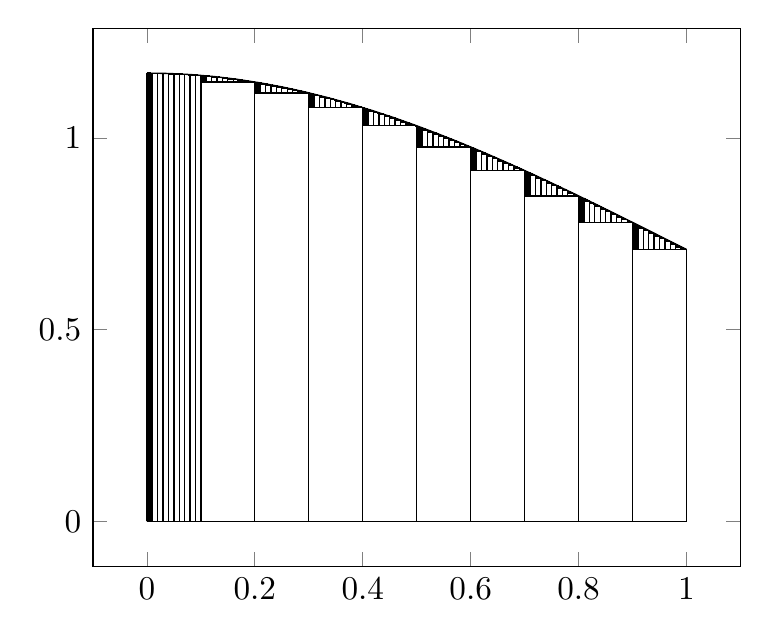
\begin{tikzpicture}[scale=1.2]
\begin{axis}
\addplot[draw=none] coordinates {(0,0)};
\addplot[domain=0:1] {e^(-x^2/2)/0.855624};
\draw (axis cs: 0, 0) -- (axis cs: 1, 0);
\draw (axis cs: 0, 0) -- (axis cs: 0, 0.7088752307384394);
\draw (axis cs: 1, 0) -- (axis cs: 1, 0.7088752307384394);
\draw (axis cs: 0, 0) -- (axis cs: 0, 1.1629085663964824);
\draw (axis cs: 1/10, 0) -- (axis cs: 1/10, 1.1629085663964824);
\draw (axis cs: 1/10, 0) -- (axis cs: 1/10, 1.145595113479829);
\draw (axis cs: 1/5, 0) -- (axis cs: 1/5, 1.145595113479829);
\draw (axis cs: 1/10, 1.145595113479829) -- (axis cs: 1/5, 1.145595113479829);
\draw (axis cs: 1/5, 0) -- (axis cs: 1/5, 1.1173102694608443);
\draw (axis cs: 3/10, 0) -- (axis cs: 3/10, 1.1173102694608443);
\draw (axis cs: 1/5, 1.1173102694608443) -- (axis cs: 3/10, 1.1173102694608443);
\draw (axis cs: 3/10, 0) -- (axis cs: 3/10, 1.07888084786895);
\draw (axis cs: 2/5, 0) -- (axis cs: 2/5, 1.07888084786895);
\draw (axis cs: 3/10, 1.07888084786895) -- (axis cs: 2/5, 1.07888084786895);
\draw (axis cs: 2/5, 0) -- (axis cs: 2/5, 1.0314073740252947);
\draw (axis cs: 1/2, 0) -- (axis cs: 1/2, 1.0314073740252947);
\draw (axis cs: 2/5, 1.0314073740252947) -- (axis cs: 1/2, 1.0314073740252947);
\draw (axis cs: 1/2, 0) -- (axis cs: 1/2, 0.9762117610727802);
\draw (axis cs: 3/5, 0) -- (axis cs: 3/5, 0.9762117610727802);
\draw (axis cs: 1/2, 0.9762117610727802) -- (axis cs: 3/5, 0.9762117610727802);
\draw (axis cs: 3/5, 0) -- (axis cs: 3/5, 0.9147762786848253);
\draw (axis cs: 7/10, 0) -- (axis cs: 7/10, 0.9147762786848253);
\draw (axis cs: 3/5, 0.9147762786848253) -- (axis cs: 7/10, 0.9147762786848253);
\draw (axis cs: 7/10, 0) -- (axis cs: 7/10, 0.848677734546616);
\draw (axis cs: 4/5, 0) -- (axis cs: 4/5, 0.848677734546616);
\draw (axis cs: 7/10, 0.848677734546616) -- (axis cs: 4/5, 0.848677734546616);
\draw (axis cs: 4/5, 0) -- (axis cs: 4/5, 0.779520924795812);
\draw (axis cs: 9/10, 0) -- (axis cs: 9/10, 0.779520924795812);
\draw (axis cs: 4/5, 0.779520924795812) -- (axis cs: 9/10, 0.779520924795812);
\draw (axis cs: 9/10, 0) -- (axis cs: 9/10, 0.7088752309073);
\draw (axis cs: 1, 0) -- (axis cs: 1, 0.7088752309073);
\draw (axis cs: 9/10, 0.7088752309073) -- (axis cs: 1, 0.7088752309073);
\draw (axis cs: 0, 0) -- (axis cs: 0, 1.1686792343954033);
\draw (axis cs: 1/100, 0) -- (axis cs: 1/100, 1.1686792343954033);
\draw (axis cs: 1/100, 0) -- (axis cs: 1/100, 1.1685039456581519);
\draw (axis cs: 1/50, 0) -- (axis cs: 1/50, 1.1685039456581519);
\draw (axis cs: 1/100, 1.1685039456581519) -- (axis cs: 1/50, 1.1685039456581519);
\draw (axis cs: 1/50, 0) -- (axis cs: 1/50, 1.1682118561849484);
\draw (axis cs: 3/100, 0) -- (axis cs: 3/100, 1.1682118561849484);
\draw (axis cs: 1/50, 1.1682118561849484) -- (axis cs: 3/100, 1.1682118561849484);
\draw (axis cs: 3/100, 0) -- (axis cs: 3/100, 1.1678030535823951);
\draw (axis cs: 1/25, 0) -- (axis cs: 1/25, 1.1678030535823951);
\draw (axis cs: 3/100, 1.1678030535823951) -- (axis cs: 1/25, 1.1678030535823951);
\draw (axis cs: 1/25, 0) -- (axis cs: 1/25, 1.1672776604315254);
\draw (axis cs: 1/20, 0) -- (axis cs: 1/20, 1.1672776604315254);
\draw (axis cs: 1/25, 1.1672776604315254) -- (axis cs: 1/20, 1.1672776604315254);
\draw (axis cs: 1/20, 0) -- (axis cs: 1/20, 1.1666358342370182);
\draw (axis cs: 3/50, 0) -- (axis cs: 3/50, 1.1666358342370182);
\draw (axis cs: 1/20, 1.1666358342370182) -- (axis cs: 3/50, 1.1666358342370182);
\draw (axis cs: 3/50, 0) -- (axis cs: 3/50, 1.165877767349838);
\draw (axis cs: 7/100, 0) -- (axis cs: 7/100, 1.165877767349838);
\draw (axis cs: 3/50, 1.165877767349838) -- (axis cs: 7/100, 1.165877767349838);
\draw (axis cs: 7/100, 0) -- (axis cs: 7/100, 1.165003686847232);
\draw (axis cs: 2/25, 0) -- (axis cs: 2/25, 1.165003686847232);
\draw (axis cs: 7/100, 1.165003686847232) -- (axis cs: 2/25, 1.165003686847232);
\draw (axis cs: 2/25, 0) -- (axis cs: 2/25, 1.1640138544527399);
\draw (axis cs: 9/100, 0) -- (axis cs: 9/100, 1.1640138544527399);
\draw (axis cs: 2/25, 1.1640138544527399) -- (axis cs: 9/100, 1.1640138544527399);
\draw (axis cs: 9/100, 0) -- (axis cs: 9/100, 1.1629085663864607);
\draw (axis cs: 1/10, 0) -- (axis cs: 1/10, 1.1629085663864607);
\draw (axis cs: 9/100, 1.1629085663864607) -- (axis cs: 1/10, 1.1629085663864607);
\draw (axis cs: 1/10, 1.145595113479829) -- (axis cs: 1/10, 1.1616881532210517);
\draw (axis cs: 11/100, 1.145595113479829) -- (axis cs: 11/100, 1.1616881532210517);
\draw (axis cs: 11/100, 1.145595113479829) -- (axis cs: 11/100, 1.1603529797348882);
\draw (axis cs: 3/25, 1.145595113479829) -- (axis cs: 3/25, 1.1603529797348882);
\draw (axis cs: 11/100, 1.1603529797348882) -- (axis cs: 3/25, 1.1603529797348882);
\draw (axis cs: 3/25, 1.145595113479829) -- (axis cs: 3/25, 1.158903444661192);
\draw (axis cs: 13/100, 1.145595113479829) -- (axis cs: 13/100, 1.158903444661192);
\draw (axis cs: 3/25, 1.158903444661192) -- (axis cs: 13/100, 1.158903444661192);
\draw (axis cs: 13/100, 1.145595113479829) -- (axis cs: 13/100, 1.1573399805893678);
\draw (axis cs: 7/50, 1.145595113479829) -- (axis cs: 7/50, 1.1573399805893678);
\draw (axis cs: 13/100, 1.1573399805893678) -- (axis cs: 7/50, 1.1573399805893678);
\draw (axis cs: 7/50, 1.145595113479829) -- (axis cs: 7/50, 1.155663053684396);
\draw (axis cs: 3/20, 1.145595113479829) -- (axis cs: 3/20, 1.155663053684396);
\draw (axis cs: 7/50, 1.155663053684396) -- (axis cs: 3/20, 1.155663053684396);
\draw (axis cs: 3/20, 1.145595113479829) -- (axis cs: 3/20, 1.1538731634752808);
\draw (axis cs: 4/25, 1.145595113479829) -- (axis cs: 4/25, 1.1538731634752808);
\draw (axis cs: 3/20, 1.1538731634752808) -- (axis cs: 4/25, 1.1538731634752808);
\draw (axis cs: 4/25, 1.145595113479829) -- (axis cs: 4/25, 1.1519708426024562);
\draw (axis cs: 17/100, 1.145595113479829) -- (axis cs: 17/100, 1.1519708426024562);
\draw (axis cs: 4/25, 1.1519708426024562) -- (axis cs: 17/100, 1.1519708426024562);
\draw (axis cs: 17/100, 1.145595113479829) -- (axis cs: 17/100, 1.1499566565550998);
\draw (axis cs: 9/50, 1.145595113479829) -- (axis cs: 9/50, 1.1499566565550998);
\draw (axis cs: 17/100, 1.1499566565550998) -- (axis cs: 9/50, 1.1499566565550998);
\draw (axis cs: 9/50, 1.145595113479829) -- (axis cs: 9/50, 1.1478312034346032);
\draw (axis cs: 19/100, 1.145595113479829) -- (axis cs: 19/100, 1.1478312034346032);
\draw (axis cs: 9/50, 1.1478312034346032) -- (axis cs: 19/100, 1.1478312034346032);
\draw (axis cs: 19/100, 1.145595113479829) -- (axis cs: 19/100, 1.14559511348866);
\draw (axis cs: 1/5, 1.145595113479829) -- (axis cs: 1/5, 1.14559511348866);
\draw (axis cs: 19/100, 1.14559511348866) -- (axis cs: 1/5, 1.14559511348866);
\draw (axis cs: 1/5, 1.1173102694608443) -- (axis cs: 1/5, 1.1432490490481584);
\draw (axis cs: 21/100, 1.1173102694608443) -- (axis cs: 21/100, 1.1432490490481584);
\draw (axis cs: 21/100, 1.1173102694608443) -- (axis cs: 21/100, 1.1407937040388867);
\draw (axis cs: 11/50, 1.1173102694608443) -- (axis cs: 11/50, 1.1407937040388867);
\draw (axis cs: 21/100, 1.1407937040388867) -- (axis cs: 11/50, 1.1407937040388867);
\draw (axis cs: 11/50, 1.1173102694608443) -- (axis cs: 11/50, 1.1382298036788177);
\draw (axis cs: 23/100, 1.1173102694608443) -- (axis cs: 23/100, 1.1382298036788177);
\draw (axis cs: 11/50, 1.1382298036788177) -- (axis cs: 23/100, 1.1382298036788177);
\draw (axis cs: 23/100, 1.1173102694608443) -- (axis cs: 23/100, 1.1355581041190577);
\draw (axis cs: 6/25, 1.1173102694608443) -- (axis cs: 6/25, 1.1355581041190577);
\draw (axis cs: 23/100, 1.1355581041190577) -- (axis cs: 6/25, 1.1355581041190577);
\draw (axis cs: 6/25, 1.1173102694608443) -- (axis cs: 6/25, 1.132779392077676);
\draw (axis cs: 1/4, 1.1173102694608443) -- (axis cs: 1/4, 1.132779392077676);
\draw (axis cs: 6/25, 1.132779392077676) -- (axis cs: 1/4, 1.132779392077676);
\draw (axis cs: 1/4, 1.1173102694608443) -- (axis cs: 1/4, 1.1298944844496572);
\draw (axis cs: 13/50, 1.1173102694608443) -- (axis cs: 13/50, 1.1298944844496572);
\draw (axis cs: 1/4, 1.1298944844496572) -- (axis cs: 13/50, 1.1298944844496572);
\draw (axis cs: 13/50, 1.1173102694608443) -- (axis cs: 13/50, 1.1269042279067734);
\draw (axis cs: 27/100, 1.1173102694608443) -- (axis cs: 27/100, 1.1269042279067734);
\draw (axis cs: 13/50, 1.1269042279067734) -- (axis cs: 27/100, 1.1269042279067734);
\draw (axis cs: 27/100, 1.1173102694608443) -- (axis cs: 27/100, 1.1238094984841474);
\draw (axis cs: 7/25, 1.1173102694608443) -- (axis cs: 7/25, 1.1238094984841474);
\draw (axis cs: 27/100, 1.1238094984841474) -- (axis cs: 7/25, 1.1238094984841474);
\draw (axis cs: 7/25, 1.1173102694608443) -- (axis cs: 7/25, 1.120611201152623);
\draw (axis cs: 29/100, 1.1173102694608443) -- (axis cs: 29/100, 1.120611201152623);
\draw (axis cs: 7/25, 1.120611201152623) -- (axis cs: 29/100, 1.120611201152623);
\draw (axis cs: 29/100, 1.1173102694608443) -- (axis cs: 29/100, 1.1173102693778385);
\draw (axis cs: 3/10, 1.1173102694608443) -- (axis cs: 3/10, 1.1173102693778385);
\draw (axis cs: 29/100, 1.1173102693778385) -- (axis cs: 3/10, 1.1173102693778385);
\draw (axis cs: 3/10, 1.07888084786895) -- (axis cs: 3/10, 1.1139076647768087);
\draw (axis cs: 31/100, 1.07888084786895) -- (axis cs: 31/100, 1.1139076647768087);
\draw (axis cs: 31/100, 1.07888084786895) -- (axis cs: 31/100, 1.110404376216082);
\draw (axis cs: 8/25, 1.07888084786895) -- (axis cs: 8/25, 1.110404376216082);
\draw (axis cs: 31/100, 1.110404376216082) -- (axis cs: 8/25, 1.110404376216082);
\draw (axis cs: 8/25, 1.07888084786895) -- (axis cs: 8/25, 1.1068014199756553);
\draw (axis cs: 33/100, 1.07888084786895) -- (axis cs: 33/100, 1.1068014199756553);
\draw (axis cs: 8/25, 1.1068014199756553) -- (axis cs: 33/100, 1.1068014199756553);
\draw (axis cs: 33/100, 1.07888084786895) -- (axis cs: 33/100, 1.1030998388359048);
\draw (axis cs: 17/50, 1.07888084786895) -- (axis cs: 17/50, 1.1030998388359048);
\draw (axis cs: 33/100, 1.1030998388359048) -- (axis cs: 17/50, 1.1030998388359048);
\draw (axis cs: 17/50, 1.07888084786895) -- (axis cs: 17/50, 1.0993007016787717);
\draw (axis cs: 7/20, 1.07888084786895) -- (axis cs: 7/20, 1.0993007016787717);
\draw (axis cs: 17/50, 1.0993007016787717) -- (axis cs: 7/20, 1.0993007016787717);
\draw (axis cs: 7/20, 1.07888084786895) -- (axis cs: 7/20, 1.0954051029736647);
\draw (axis cs: 9/25, 1.07888084786895) -- (axis cs: 9/25, 1.0954051029736647);
\draw (axis cs: 7/20, 1.0954051029736647) -- (axis cs: 9/25, 1.0954051029736647);
\draw (axis cs: 9/25, 1.07888084786895) -- (axis cs: 9/25, 1.0914141622523388);
\draw (axis cs: 37/100, 1.07888084786895) -- (axis cs: 37/100, 1.0914141622523388);
\draw (axis cs: 9/25, 1.0914141622523388) -- (axis cs: 37/100, 1.0914141622523388);
\draw (axis cs: 37/100, 1.07888084786895) -- (axis cs: 37/100, 1.087329023573098);
\draw (axis cs: 19/50, 1.07888084786895) -- (axis cs: 19/50, 1.087329023573098);
\draw (axis cs: 37/100, 1.087329023573098) -- (axis cs: 19/50, 1.087329023573098);
\draw (axis cs: 19/50, 1.07888084786895) -- (axis cs: 19/50, 1.0831508549713462);
\draw (axis cs: 39/100, 1.07888084786895) -- (axis cs: 39/100, 1.0831508549713462);
\draw (axis cs: 19/50, 1.0831508549713462) -- (axis cs: 39/100, 1.0831508549713462);
\draw (axis cs: 39/100, 1.07888084786895) -- (axis cs: 39/100, 1.0788808479124965);
\draw (axis cs: 2/5, 1.07888084786895) -- (axis cs: 2/5, 1.0788808479124965);
\draw (axis cs: 39/100, 1.0788808479124965) -- (axis cs: 2/5, 1.0788808479124965);
\draw (axis cs: 2/5, 1.0314073740252947) -- (axis cs: 2/5, 1.0745202167192769);
\draw (axis cs: 41/100, 1.0314073740252947) -- (axis cs: 41/100, 1.0745202167192769);
\draw (axis cs: 41/100, 1.0314073740252947) -- (axis cs: 41/100, 1.0700701979974419);
\draw (axis cs: 21/50, 1.0314073740252947) -- (axis cs: 21/50, 1.0700701979974419);
\draw (axis cs: 41/100, 1.0700701979974419) -- (axis cs: 21/50, 1.0700701979974419);
\draw (axis cs: 21/50, 1.0314073740252947) -- (axis cs: 21/50, 1.0655320500529688);
\draw (axis cs: 43/100, 1.0314073740252947) -- (axis cs: 43/100, 1.0655320500529688);
\draw (axis cs: 21/50, 1.0655320500529688) -- (axis cs: 43/100, 1.0655320500529688);
\draw (axis cs: 43/100, 1.0314073740252947) -- (axis cs: 43/100, 1.06090705229995);
\draw (axis cs: 11/25, 1.0314073740252947) -- (axis cs: 11/25, 1.06090705229995);
\draw (axis cs: 43/100, 1.06090705229995) -- (axis cs: 11/25, 1.06090705229995);
\draw (axis cs: 11/25, 1.0314073740252947) -- (axis cs: 11/25, 1.0561965046604347);
\draw (axis cs: 9/20, 1.0314073740252947) -- (axis cs: 9/20, 1.0561965046604347);
\draw (axis cs: 11/25, 1.0561965046604347) -- (axis cs: 9/20, 1.0561965046604347);
\draw (axis cs: 9/20, 1.0314073740252947) -- (axis cs: 9/20, 1.051401726956616);
\draw (axis cs: 23/50, 1.0314073740252947) -- (axis cs: 23/50, 1.051401726956616);
\draw (axis cs: 9/20, 1.051401726956616) -- (axis cs: 23/50, 1.051401726956616);
\draw (axis cs: 23/50, 1.0314073740252947) -- (axis cs: 23/50, 1.0465240582957578);
\draw (axis cs: 47/100, 1.0314073740252947) -- (axis cs: 47/100, 1.0465240582957578);
\draw (axis cs: 23/50, 1.0465240582957578) -- (axis cs: 47/100, 1.0465240582957578);
\draw (axis cs: 47/100, 1.0314073740252947) -- (axis cs: 47/100, 1.0415648564482645);
\draw (axis cs: 12/25, 1.0314073740252947) -- (axis cs: 12/25, 1.0415648564482645);
\draw (axis cs: 47/100, 1.0415648564482645) -- (axis cs: 12/25, 1.0415648564482645);
\draw (axis cs: 12/25, 1.0314073740252947) -- (axis cs: 12/25, 1.0365254972192939);
\draw (axis cs: 49/100, 1.0314073740252947) -- (axis cs: 49/100, 1.0365254972192939);
\draw (axis cs: 12/25, 1.0365254972192939) -- (axis cs: 49/100, 1.0365254972192939);
\draw (axis cs: 49/100, 1.0314073740252947) -- (axis cs: 49/100, 1.031407373814324);
\draw (axis cs: 1/2, 1.0314073740252947) -- (axis cs: 1/2, 1.031407373814324);
\draw (axis cs: 49/100, 1.031407373814324) -- (axis cs: 1/2, 1.031407373814324);
\draw (axis cs: 1/2, 0.9762117610727802) -- (axis cs: 1/2, 1.0262118964712261);
\draw (axis cs: 51/100, 0.9762117610727802) -- (axis cs: 51/100, 1.0262118964712261);
\draw (axis cs: 51/100, 0.9762117610727802) -- (axis cs: 51/100, 1.0209404907355755);
\draw (axis cs: 13/25, 0.9762117610727802) -- (axis cs: 13/25, 1.0209404907355755);
\draw (axis cs: 51/100, 1.0209404907355755) -- (axis cs: 13/25, 1.0209404907355755);
\draw (axis cs: 13/25, 0.9762117610727802) -- (axis cs: 13/25, 1.0155945984158463);
\draw (axis cs: 53/100, 0.9762117610727802) -- (axis cs: 53/100, 1.0155945984158463);
\draw (axis cs: 13/25, 1.0155945984158463) -- (axis cs: 53/100, 1.0155945984158463);
\draw (axis cs: 53/100, 0.9762117610727802) -- (axis cs: 53/100, 1.010175675867788);
\draw (axis cs: 27/50, 0.9762117610727802) -- (axis cs: 27/50, 1.010175675867788);
\draw (axis cs: 53/100, 1.010175675867788) -- (axis cs: 27/50, 1.010175675867788);
\draw (axis cs: 27/50, 0.9762117610727802) -- (axis cs: 27/50, 1.0046851935989134);
\draw (axis cs: 11/20, 0.9762117610727802) -- (axis cs: 11/20, 1.0046851935989134);
\draw (axis cs: 27/50, 1.0046851935989134) -- (axis cs: 11/20, 1.0046851935989134);
\draw (axis cs: 11/20, 0.9762117610727802) -- (axis cs: 11/20, 0.9991246356064033);
\draw (axis cs: 14/25, 0.9762117610727802) -- (axis cs: 14/25, 0.9991246356064033);
\draw (axis cs: 11/20, 0.9991246356064033) -- (axis cs: 14/25, 0.9991246356064033);
\draw (axis cs: 14/25, 0.9762117610727802) -- (axis cs: 14/25, 0.9934954987118504);
\draw (axis cs: 57/100, 0.9762117610727802) -- (axis cs: 57/100, 0.9934954987118504);
\draw (axis cs: 14/25, 0.9934954987118504) -- (axis cs: 57/100, 0.9934954987118504);
\draw (axis cs: 57/100, 0.9762117610727802) -- (axis cs: 57/100, 0.9877992918932575);
\draw (axis cs: 29/50, 0.9762117610727802) -- (axis cs: 29/50, 0.9877992918932575);
\draw (axis cs: 57/100, 0.9877992918932575) -- (axis cs: 29/50, 0.9877992918932575);
\draw (axis cs: 29/50, 0.9762117610727802) -- (axis cs: 29/50, 0.9820375356147064);
\draw (axis cs: 59/100, 0.9762117610727802) -- (axis cs: 59/100, 0.9820375356147064);
\draw (axis cs: 29/50, 0.9820375356147064) -- (axis cs: 59/100, 0.9820375356147064);
\draw (axis cs: 59/100, 0.9762117610727802) -- (axis cs: 59/100, 0.9762117611541081);
\draw (axis cs: 3/5, 0.9762117610727802) -- (axis cs: 3/5, 0.9762117611541081);
\draw (axis cs: 59/100, 0.9762117611541081) -- (axis cs: 3/5, 0.9762117611541081);
\draw (axis cs: 3/5, 0.9147762786848253) -- (axis cs: 3/5, 0.9703235099294532);
\draw (axis cs: 61/100, 0.9147762786848253) -- (axis cs: 61/100, 0.9703235099294532);
\draw (axis cs: 61/100, 0.9147762786848253) -- (axis cs: 61/100, 0.9643743328239671);
\draw (axis cs: 31/50, 0.9147762786848253) -- (axis cs: 31/50, 0.9643743328239671);
\draw (axis cs: 61/100, 0.9643743328239671) -- (axis cs: 31/50, 0.9643743328239671);
\draw (axis cs: 31/50, 0.9147762786848253) -- (axis cs: 31/50, 0.9583657895072194);
\draw (axis cs: 63/100, 0.9147762786848253) -- (axis cs: 63/100, 0.9583657895072194);
\draw (axis cs: 31/50, 0.9583657895072194) -- (axis cs: 63/100, 0.9583657895072194);
\draw (axis cs: 63/100, 0.9147762786848253) -- (axis cs: 63/100, 0.9522994477666723);
\draw (axis cs: 16/25, 0.9147762786848253) -- (axis cs: 16/25, 0.9522994477666723);
\draw (axis cs: 63/100, 0.9522994477666723) -- (axis cs: 16/25, 0.9522994477666723);
\draw (axis cs: 16/25, 0.9147762786848253) -- (axis cs: 16/25, 0.9461768828300766);
\draw (axis cs: 13/20, 0.9147762786848253) -- (axis cs: 13/20, 0.9461768828300766);
\draw (axis cs: 16/25, 0.9461768828300766) -- (axis cs: 13/20, 0.9461768828300766);
\draw (axis cs: 13/20, 0.9147762786848253) -- (axis cs: 13/20, 0.939999676685661);
\draw (axis cs: 33/50, 0.9147762786848253) -- (axis cs: 33/50, 0.939999676685661);
\draw (axis cs: 13/20, 0.939999676685661) -- (axis cs: 33/50, 0.939999676685661);
\draw (axis cs: 33/50, 0.9147762786848253) -- (axis cs: 33/50, 0.9337694174105843);
\draw (axis cs: 67/100, 0.9147762786848253) -- (axis cs: 67/100, 0.9337694174105843);
\draw (axis cs: 33/50, 0.9337694174105843) -- (axis cs: 67/100, 0.9337694174105843);
\draw (axis cs: 67/100, 0.9147762786848253) -- (axis cs: 67/100, 0.9274876984980764);
\draw (axis cs: 17/25, 0.9147762786848253) -- (axis cs: 17/25, 0.9274876984980764);
\draw (axis cs: 67/100, 0.9274876984980764) -- (axis cs: 17/25, 0.9274876984980764);
\draw (axis cs: 17/25, 0.9147762786848253) -- (axis cs: 17/25, 0.9211561181863079);
\draw (axis cs: 69/100, 0.9147762786848253) -- (axis cs: 69/100, 0.9211561181863079);
\draw (axis cs: 17/25, 0.9211561181863079) -- (axis cs: 69/100, 0.9211561181863079);
\draw (axis cs: 69/100, 0.9147762786848253) -- (axis cs: 69/100, 0.9147762787893747);
\draw (axis cs: 7/10, 0.9147762786848253) -- (axis cs: 7/10, 0.9147762787893747);
\draw (axis cs: 69/100, 0.9147762787893747) -- (axis cs: 7/10, 0.9147762787893747);
\draw (axis cs: 7/10, 0.848677734546616) -- (axis cs: 7/10, 0.9083497860307876);
\draw (axis cs: 71/100, 0.848677734546616) -- (axis cs: 71/100, 0.9083497860307876);
\draw (axis cs: 71/100, 0.848677734546616) -- (axis cs: 71/100, 0.9018782483798445);
\draw (axis cs: 18/25, 0.848677734546616) -- (axis cs: 18/25, 0.9018782483798445);
\draw (axis cs: 71/100, 0.9018782483798445) -- (axis cs: 18/25, 0.9018782483798445);
\draw (axis cs: 18/25, 0.848677734546616) -- (axis cs: 18/25, 0.8953632763912646);
\draw (axis cs: 73/100, 0.848677734546616) -- (axis cs: 73/100, 0.8953632763912646);
\draw (axis cs: 18/25, 0.8953632763912646) -- (axis cs: 73/100, 0.8953632763912646);
\draw (axis cs: 73/100, 0.848677734546616) -- (axis cs: 73/100, 0.8888064820484545);
\draw (axis cs: 37/50, 0.848677734546616) -- (axis cs: 37/50, 0.8888064820484545);
\draw (axis cs: 73/100, 0.8888064820484545) -- (axis cs: 37/50, 0.8888064820484545);
\draw (axis cs: 37/50, 0.848677734546616) -- (axis cs: 37/50, 0.8822094781107758);
\draw (axis cs: 3/4, 0.848677734546616) -- (axis cs: 3/4, 0.8822094781107758);
\draw (axis cs: 37/50, 0.8822094781107758) -- (axis cs: 3/4, 0.8822094781107758);
\draw (axis cs: 3/4, 0.848677734546616) -- (axis cs: 3/4, 0.8755738774651708);
\draw (axis cs: 19/25, 0.848677734546616) -- (axis cs: 19/25, 0.8755738774651708);
\draw (axis cs: 3/4, 0.8755738774651708) -- (axis cs: 19/25, 0.8755738774651708);
\draw (axis cs: 19/25, 0.848677734546616) -- (axis cs: 19/25, 0.868901292482507);
\draw (axis cs: 77/100, 0.848677734546616) -- (axis cs: 77/100, 0.868901292482507);
\draw (axis cs: 19/25, 0.868901292482507) -- (axis cs: 77/100, 0.868901292482507);
\draw (axis cs: 77/100, 0.848677734546616) -- (axis cs: 77/100, 0.8621933343789866);
\draw (axis cs: 39/50, 0.848677734546616) -- (axis cs: 39/50, 0.8621933343789866);
\draw (axis cs: 77/100, 0.8621933343789866) -- (axis cs: 39/50, 0.8621933343789866);
\draw (axis cs: 39/50, 0.848677734546616) -- (axis cs: 39/50, 0.8554516125829663);
\draw (axis cs: 79/100, 0.848677734546616) -- (axis cs: 79/100, 0.8554516125829663);
\draw (axis cs: 39/50, 0.8554516125829663) -- (axis cs: 79/100, 0.8554516125829663);
\draw (axis cs: 79/100, 0.848677734546616) -- (axis cs: 79/100, 0.8486777341075245);
\draw (axis cs: 4/5, 0.848677734546616) -- (axis cs: 4/5, 0.8486777341075245);
\draw (axis cs: 79/100, 0.8486777341075245) -- (axis cs: 4/5, 0.8486777341075245);
\draw (axis cs: 4/5, 0.779520924795812) -- (axis cs: 4/5, 0.8418733029291042);
\draw (axis cs: 81/100, 0.779520924795812) -- (axis cs: 81/100, 0.8418733029291042);
\draw (axis cs: 81/100, 0.779520924795812) -- (axis cs: 81/100, 0.8350399193725604);
\draw (axis cs: 41/50, 0.779520924795812) -- (axis cs: 41/50, 0.8350399193725604);
\draw (axis cs: 81/100, 0.8350399193725604) -- (axis cs: 41/50, 0.8350399193725604);
\draw (axis cs: 41/50, 0.779520924795812) -- (axis cs: 41/50, 0.8281791800803281);
\draw (axis cs: 83/100, 0.779520924795812) -- (axis cs: 83/100, 0.8281791800803281);
\draw (axis cs: 41/50, 0.8281791800803281) -- (axis cs: 83/100, 0.8281791800803281);
\draw (axis cs: 83/100, 0.779520924795812) -- (axis cs: 83/100, 0.8212926751105863);
\draw (axis cs: 21/25, 0.779520924795812) -- (axis cs: 21/25, 0.8212926751105863);
\draw (axis cs: 83/100, 0.8212926751105863) -- (axis cs: 21/25, 0.8212926751105863);
\draw (axis cs: 21/25, 0.779520924795812) -- (axis cs: 21/25, 0.8143819907807417);
\draw (axis cs: 17/20, 0.779520924795812) -- (axis cs: 17/20, 0.8143819907807417);
\draw (axis cs: 21/25, 0.8143819907807417) -- (axis cs: 17/20, 0.8143819907807417);
\draw (axis cs: 17/20, 0.779520924795812) -- (axis cs: 17/20, 0.807448706798706);
\draw (axis cs: 43/50, 0.779520924795812) -- (axis cs: 43/50, 0.807448706798706);
\draw (axis cs: 17/20, 0.807448706798706) -- (axis cs: 43/50, 0.807448706798706);
\draw (axis cs: 43/50, 0.779520924795812) -- (axis cs: 43/50, 0.8004943962528822);
\draw (axis cs: 87/100, 0.779520924795812) -- (axis cs: 87/100, 0.8004943962528822);
\draw (axis cs: 43/50, 0.8004943962528822) -- (axis cs: 87/100, 0.8004943962528822);
\draw (axis cs: 87/100, 0.779520924795812) -- (axis cs: 87/100, 0.793520625042011);
\draw (axis cs: 22/25, 0.779520924795812) -- (axis cs: 22/25, 0.793520625042011);
\draw (axis cs: 87/100, 0.793520625042011) -- (axis cs: 22/25, 0.793520625042011);
\draw (axis cs: 22/25, 0.779520924795812) -- (axis cs: 22/25, 0.7865289513134806);
\draw (axis cs: 89/100, 0.779520924795812) -- (axis cs: 89/100, 0.7865289513134806);
\draw (axis cs: 22/25, 0.7865289513134806) -- (axis cs: 89/100, 0.7865289513134806);
\draw (axis cs: 89/100, 0.779520924795812) -- (axis cs: 89/100, 0.779520924910358);
\draw (axis cs: 9/10, 0.779520924795812) -- (axis cs: 9/10, 0.779520924910358);
\draw (axis cs: 89/100, 0.779520924910358) -- (axis cs: 9/10, 0.779520924910358);
\draw (axis cs: 9/10, 0.7088752309073) -- (axis cs: 9/10, 0.772498086827401);
\draw (axis cs: 91/100, 0.7088752309073) -- (axis cs: 91/100, 0.772498086827401);
\draw (axis cs: 91/100, 0.7088752309073) -- (axis cs: 91/100, 0.7654619686762921);
\draw (axis cs: 23/25, 0.7088752309073) -- (axis cs: 23/25, 0.7654619686762921);
\draw (axis cs: 91/100, 0.7654619686762921) -- (axis cs: 23/25, 0.7654619686762921);
\draw (axis cs: 23/25, 0.7088752309073) -- (axis cs: 23/25, 0.7584140921603341);
\draw (axis cs: 93/100, 0.7088752309073) -- (axis cs: 93/100, 0.7584140921603341);
\draw (axis cs: 23/25, 0.7584140921603341) -- (axis cs: 93/100, 0.7584140921603341);
\draw (axis cs: 93/100, 0.7088752309073) -- (axis cs: 93/100, 0.7513559685588359);
\draw (axis cs: 47/50, 0.7088752309073) -- (axis cs: 47/50, 0.7513559685588359);
\draw (axis cs: 93/100, 0.7513559685588359) -- (axis cs: 47/50, 0.7513559685588359);
\draw (axis cs: 47/50, 0.7088752309073) -- (axis cs: 47/50, 0.7442890982214072);
\draw (axis cs: 19/20, 0.7088752309073) -- (axis cs: 19/20, 0.7442890982214072);
\draw (axis cs: 47/50, 0.7442890982214072) -- (axis cs: 19/20, 0.7442890982214072);
\draw (axis cs: 19/20, 0.7088752309073) -- (axis cs: 19/20, 0.7372149700723738);
\draw (axis cs: 24/25, 0.7088752309073) -- (axis cs: 24/25, 0.7372149700723738);
\draw (axis cs: 19/20, 0.7372149700723738) -- (axis cs: 24/25, 0.7372149700723738);
\draw (axis cs: 24/25, 0.7088752309073) -- (axis cs: 24/25, 0.7301350611255129);
\draw (axis cs: 97/100, 0.7088752309073) -- (axis cs: 97/100, 0.7301350611255129);
\draw (axis cs: 24/25, 0.7301350611255129) -- (axis cs: 97/100, 0.7301350611255129);
\draw (axis cs: 97/100, 0.7088752309073) -- (axis cs: 97/100, 0.7230508360093055);
\draw (axis cs: 49/50, 0.7088752309073) -- (axis cs: 49/50, 0.7230508360093055);
\draw (axis cs: 97/100, 0.7230508360093055) -- (axis cs: 49/50, 0.7230508360093055);
\draw (axis cs: 49/50, 0.7088752309073) -- (axis cs: 49/50, 0.7159637465028859);
\draw (axis cs: 99/100, 0.7088752309073) -- (axis cs: 99/100, 0.7159637465028859);
\draw (axis cs: 49/50, 0.7159637465028859) -- (axis cs: 99/100, 0.7159637465028859);
\draw (axis cs: 99/100, 0.7088752309073) -- (axis cs: 99/100, 0.7088752310828618);
\draw (axis cs: 1, 0.7088752309073) -- (axis cs: 1, 0.7088752310828618);
\draw (axis cs: 99/100, 0.7088752310828618) -- (axis cs: 1, 0.7088752310828618);
\draw (axis cs: 0, 0) -- (axis cs: 0, 1.16873708544891);
\draw (axis cs: 1/1000, 0) -- (axis cs: 1/1000, 1.16873708544891);
\draw (axis cs: 1/1000, 0) -- (axis cs: 1/1000, 1.1687353323446097);
\draw (axis cs: 1/500, 0) -- (axis cs: 1/500, 1.1687353323446097);
\draw (axis cs: 1/1000, 1.1687353323446097) -- (axis cs: 1/500, 1.1687353323446097);
\draw (axis cs: 1/500, 0) -- (axis cs: 1/500, 1.1687324105099877);
\draw (axis cs: 3/1000, 0) -- (axis cs: 3/1000, 1.1687324105099877);
\draw (axis cs: 1/500, 1.1687324105099877) -- (axis cs: 3/1000, 1.1687324105099877);
\draw (axis cs: 3/1000, 0) -- (axis cs: 3/1000, 1.1687283199537377);
\draw (axis cs: 1/250, 0) -- (axis cs: 1/250, 1.1687283199537377);
\draw (axis cs: 3/1000, 1.1687283199537377) -- (axis cs: 1/250, 1.1687283199537377);
\draw (axis cs: 1/250, 0) -- (axis cs: 1/250, 1.1687230606881593);
\draw (axis cs: 1/200, 0) -- (axis cs: 1/200, 1.1687230606881593);
\draw (axis cs: 1/250, 1.1687230606881593) -- (axis cs: 1/200, 1.1687230606881593);
\draw (axis cs: 1/200, 0) -- (axis cs: 1/200, 1.1687166327290237);
\draw (axis cs: 3/500, 0) -- (axis cs: 3/500, 1.1687166327290237);
\draw (axis cs: 1/200, 1.1687166327290237) -- (axis cs: 3/500, 1.1687166327290237);
\draw (axis cs: 3/500, 0) -- (axis cs: 3/500, 1.1687090360956192);
\draw (axis cs: 7/1000, 0) -- (axis cs: 7/1000, 1.1687090360956192);
\draw (axis cs: 3/500, 1.1687090360956192) -- (axis cs: 7/1000, 1.1687090360956192);
\draw (axis cs: 7/1000, 0) -- (axis cs: 7/1000, 1.1687002708107348);
\draw (axis cs: 1/125, 0) -- (axis cs: 1/125, 1.1687002708107348);
\draw (axis cs: 7/1000, 1.1687002708107348) -- (axis cs: 1/125, 1.1687002708107348);
\draw (axis cs: 1/125, 0) -- (axis cs: 1/125, 1.1686903369006665);
\draw (axis cs: 9/1000, 0) -- (axis cs: 9/1000, 1.1686903369006665);
\draw (axis cs: 1/125, 1.1686903369006665) -- (axis cs: 9/1000, 1.1686903369006665);
\draw (axis cs: 9/1000, 0) -- (axis cs: 9/1000, 1.1686792343954484);
\draw (axis cs: 1/100, 0) -- (axis cs: 1/100, 1.1686792343954484);
\draw (axis cs: 9/1000, 1.1686792343954484) -- (axis cs: 1/100, 1.1686792343954484);
\draw (axis cs: 1/100, 1.1685039456581519) -- (axis cs: 1/100, 1.1686669633279563);
\draw (axis cs: 11/1000, 1.1685039456581519) -- (axis cs: 11/1000, 1.1686669633279563);
\draw (axis cs: 11/1000, 1.1685039456581519) -- (axis cs: 11/1000, 1.1686535237352018);
\draw (axis cs: 3/250, 1.1685039456581519) -- (axis cs: 3/250, 1.1686535237352018);
\draw (axis cs: 11/1000, 1.1686535237352018) -- (axis cs: 3/250, 1.1686535237352018);
\draw (axis cs: 3/250, 1.1685039456581519) -- (axis cs: 3/250, 1.1686389156575014);
\draw (axis cs: 13/1000, 1.1685039456581519) -- (axis cs: 13/1000, 1.1686389156575014);
\draw (axis cs: 3/250, 1.1686389156575014) -- (axis cs: 13/1000, 1.1686389156575014);
\draw (axis cs: 13/1000, 1.1685039456581519) -- (axis cs: 13/1000, 1.1686231391386777);
\draw (axis cs: 7/500, 1.1685039456581519) -- (axis cs: 7/500, 1.1686231391386777);
\draw (axis cs: 13/1000, 1.1686231391386777) -- (axis cs: 7/500, 1.1686231391386777);
\draw (axis cs: 7/500, 1.1685039456581519) -- (axis cs: 7/500, 1.1686061942260435);
\draw (axis cs: 3/200, 1.1685039456581519) -- (axis cs: 3/200, 1.1686061942260435);
\draw (axis cs: 7/500, 1.1686061942260435) -- (axis cs: 3/200, 1.1686061942260435);
\draw (axis cs: 3/200, 1.1685039456581519) -- (axis cs: 3/200, 1.1685880809704374);
\draw (axis cs: 2/125, 1.1685039456581519) -- (axis cs: 2/125, 1.1685880809704374);
\draw (axis cs: 3/200, 1.1685880809704374) -- (axis cs: 2/125, 1.1685880809704374);
\draw (axis cs: 2/125, 1.1685039456581519) -- (axis cs: 2/125, 1.1685687994261984);
\draw (axis cs: 17/1000, 1.1685039456581519) -- (axis cs: 17/1000, 1.1685687994261984);
\draw (axis cs: 2/125, 1.1685687994261984) -- (axis cs: 17/1000, 1.1685687994261984);
\draw (axis cs: 17/1000, 1.1685039456581519) -- (axis cs: 17/1000, 1.168548349651166);
\draw (axis cs: 9/500, 1.1685039456581519) -- (axis cs: 9/500, 1.168548349651166);
\draw (axis cs: 17/1000, 1.168548349651166) -- (axis cs: 9/500, 1.168548349651166);
\draw (axis cs: 9/500, 1.1685039456581519) -- (axis cs: 9/500, 1.1685267317066834);
\draw (axis cs: 19/1000, 1.1685039456581519) -- (axis cs: 19/1000, 1.1685267317066834);
\draw (axis cs: 9/500, 1.1685267317066834) -- (axis cs: 19/1000, 1.1685267317066834);
\draw (axis cs: 19/1000, 1.1685039456581519) -- (axis cs: 19/1000, 1.1685039456575965);
\draw (axis cs: 1/50, 1.1685039456581519) -- (axis cs: 1/50, 1.1685039456575965);
\draw (axis cs: 19/1000, 1.1685039456575965) -- (axis cs: 1/50, 1.1685039456575965);
\draw (axis cs: 1/50, 1.1682118561849484) -- (axis cs: 1/50, 1.1684799915722552);
\draw (axis cs: 21/1000, 1.1682118561849484) -- (axis cs: 21/1000, 1.1684799915722552);
\draw (axis cs: 21/1000, 1.1682118561849484) -- (axis cs: 21/1000, 1.1684548695233343);
\draw (axis cs: 11/500, 1.1682118561849484) -- (axis cs: 11/500, 1.1684548695233343);
\draw (axis cs: 21/1000, 1.1684548695233343) -- (axis cs: 11/500, 1.1684548695233343);
\draw (axis cs: 11/500, 1.1682118561849484) -- (axis cs: 11/500, 1.168428579584607);
\draw (axis cs: 23/1000, 1.1682118561849484) -- (axis cs: 23/1000, 1.168428579584607);
\draw (axis cs: 11/500, 1.168428579584607) -- (axis cs: 23/1000, 1.168428579584607);
\draw (axis cs: 23/1000, 1.1682118561849484) -- (axis cs: 23/1000, 1.168401121835691);
\draw (axis cs: 3/125, 1.1682118561849484) -- (axis cs: 3/125, 1.168401121835691);
\draw (axis cs: 23/1000, 1.168401121835691) -- (axis cs: 3/125, 1.168401121835691);
\draw (axis cs: 3/125, 1.1682118561849484) -- (axis cs: 3/125, 1.1683724963589435);
\draw (axis cs: 1/40, 1.1682118561849484) -- (axis cs: 1/40, 1.1683724963589435);
\draw (axis cs: 3/125, 1.1683724963589435) -- (axis cs: 1/40, 1.1683724963589435);
\draw (axis cs: 1/40, 1.1682118561849484) -- (axis cs: 1/40, 1.1683427032402243);
\draw (axis cs: 13/500, 1.1682118561849484) -- (axis cs: 13/500, 1.1683427032402243);
\draw (axis cs: 1/40, 1.1683427032402243) -- (axis cs: 13/500, 1.1683427032402243);
\draw (axis cs: 13/500, 1.1682118561849484) -- (axis cs: 13/500, 1.1683117425688934);
\draw (axis cs: 27/1000, 1.1682118561849484) -- (axis cs: 27/1000, 1.1683117425688934);
\draw (axis cs: 13/500, 1.1683117425688934) -- (axis cs: 27/1000, 1.1683117425688934);
\draw (axis cs: 27/1000, 1.1682118561849484) -- (axis cs: 27/1000, 1.1682796144378107);
\draw (axis cs: 7/250, 1.1682118561849484) -- (axis cs: 7/250, 1.1682796144378107);
\draw (axis cs: 27/1000, 1.1682796144378107) -- (axis cs: 7/250, 1.1682796144378107);
\draw (axis cs: 7/250, 1.1682118561849484) -- (axis cs: 7/250, 1.1682463189433363);
\draw (axis cs: 29/1000, 1.1682118561849484) -- (axis cs: 29/1000, 1.1682463189433363);
\draw (axis cs: 7/250, 1.1682463189433363) -- (axis cs: 29/1000, 1.1682463189433363);
\draw (axis cs: 29/1000, 1.1682118561849484) -- (axis cs: 29/1000, 1.1682118561853019);
\draw (axis cs: 3/100, 1.1682118561849484) -- (axis cs: 3/100, 1.1682118561853019);
\draw (axis cs: 29/1000, 1.1682118561853019) -- (axis cs: 3/100, 1.1682118561853019);
\draw (axis cs: 3/100, 1.1678030535823951) -- (axis cs: 3/100, 1.1681762262670843);
\draw (axis cs: 31/1000, 1.1678030535823951) -- (axis cs: 31/1000, 1.1681762262670843);
\draw (axis cs: 31/1000, 1.1678030535823951) -- (axis cs: 31/1000, 1.168139429295547);
\draw (axis cs: 4/125, 1.1678030535823951) -- (axis cs: 4/125, 1.168139429295547);
\draw (axis cs: 31/1000, 1.168139429295547) -- (axis cs: 4/125, 1.168139429295547);
\draw (axis cs: 4/125, 1.1678030535823951) -- (axis cs: 4/125, 1.168101465381044);
\draw (axis cs: 33/1000, 1.1678030535823951) -- (axis cs: 33/1000, 1.168101465381044);
\draw (axis cs: 4/125, 1.168101465381044) -- (axis cs: 33/1000, 1.168101465381044);
\draw (axis cs: 33/1000, 1.1678030535823951) -- (axis cs: 33/1000, 1.1680623346374273);
\draw (axis cs: 17/500, 1.1678030535823951) -- (axis cs: 17/500, 1.1680623346374273);
\draw (axis cs: 33/1000, 1.1680623346374273) -- (axis cs: 17/500, 1.1680623346374273);
\draw (axis cs: 17/500, 1.1678030535823951) -- (axis cs: 17/500, 1.1680220371820451);
\draw (axis cs: 7/200, 1.1678030535823951) -- (axis cs: 7/200, 1.1680220371820451);
\draw (axis cs: 17/500, 1.1680220371820451) -- (axis cs: 7/200, 1.1680220371820451);
\draw (axis cs: 7/200, 1.1678030535823951) -- (axis cs: 7/200, 1.1679805731357418);
\draw (axis cs: 9/250, 1.1678030535823951) -- (axis cs: 9/250, 1.1679805731357418);
\draw (axis cs: 7/200, 1.1679805731357418) -- (axis cs: 9/250, 1.1679805731357418);
\draw (axis cs: 9/250, 1.1678030535823951) -- (axis cs: 9/250, 1.1679379426228567);
\draw (axis cs: 37/1000, 1.1678030535823951) -- (axis cs: 37/1000, 1.1679379426228567);
\draw (axis cs: 9/250, 1.1679379426228567) -- (axis cs: 37/1000, 1.1679379426228567);
\draw (axis cs: 37/1000, 1.1678030535823951) -- (axis cs: 37/1000, 1.167894145771225);
\draw (axis cs: 19/500, 1.1678030535823951) -- (axis cs: 19/500, 1.167894145771225);
\draw (axis cs: 37/1000, 1.167894145771225) -- (axis cs: 19/500, 1.167894145771225);
\draw (axis cs: 19/500, 1.1678030535823951) -- (axis cs: 19/500, 1.1678491827121757);
\draw (axis cs: 39/1000, 1.1678030535823951) -- (axis cs: 39/1000, 1.1678491827121757);
\draw (axis cs: 19/500, 1.1678491827121757) -- (axis cs: 39/1000, 1.1678491827121757);
\draw (axis cs: 39/1000, 1.1678030535823951) -- (axis cs: 39/1000, 1.1678030535805308);
\draw (axis cs: 1/25, 1.1678030535823951) -- (axis cs: 1/25, 1.1678030535805308);
\draw (axis cs: 39/1000, 1.1678030535805308) -- (axis cs: 1/25, 1.1678030535805308);
\draw (axis cs: 1/25, 1.1672776604315254) -- (axis cs: 1/25, 1.167755758514606);
\draw (axis cs: 41/1000, 1.1672776604315254) -- (axis cs: 41/1000, 1.167755758514606);
\draw (axis cs: 41/1000, 1.1672776604315254) -- (axis cs: 41/1000, 1.1677072976587588);
\draw (axis cs: 21/500, 1.1672776604315254) -- (axis cs: 21/500, 1.1677072976587588);
\draw (axis cs: 41/1000, 1.1677072976587588) -- (axis cs: 21/500, 1.1677072976587588);
\draw (axis cs: 21/500, 1.1672776604315254) -- (axis cs: 21/500, 1.1676576711532989);
\draw (axis cs: 43/1000, 1.1672776604315254) -- (axis cs: 43/1000, 1.1676576711532989);
\draw (axis cs: 21/500, 1.1676576711532989) -- (axis cs: 43/1000, 1.1676576711532989);
\draw (axis cs: 43/1000, 1.1672776604315254) -- (axis cs: 43/1000, 1.1676068791494576);
\draw (axis cs: 11/250, 1.1672776604315254) -- (axis cs: 11/250, 1.1676068791494576);
\draw (axis cs: 43/1000, 1.1676068791494576) -- (axis cs: 11/250, 1.1676068791494576);
\draw (axis cs: 11/250, 1.1672776604315254) -- (axis cs: 11/250, 1.167554921799515);
\draw (axis cs: 9/200, 1.1672776604315254) -- (axis cs: 9/200, 1.167554921799515);
\draw (axis cs: 11/250, 1.167554921799515) -- (axis cs: 9/200, 1.167554921799515);
\draw (axis cs: 9/200, 1.1672776604315254) -- (axis cs: 9/200, 1.16750179925924);
\draw (axis cs: 23/500, 1.1672776604315254) -- (axis cs: 23/500, 1.16750179925924);
\draw (axis cs: 9/200, 1.16750179925924) -- (axis cs: 23/500, 1.16750179925924);
\draw (axis cs: 23/500, 1.1672776604315254) -- (axis cs: 23/500, 1.16744751168789);
\draw (axis cs: 47/1000, 1.1672776604315254) -- (axis cs: 47/1000, 1.16744751168789);
\draw (axis cs: 23/500, 1.16744751168789) -- (axis cs: 47/1000, 1.16744751168789);
\draw (axis cs: 47/1000, 1.1672776604315254) -- (axis cs: 47/1000, 1.1673920592482105);
\draw (axis cs: 6/125, 1.1672776604315254) -- (axis cs: 6/125, 1.1673920592482105);
\draw (axis cs: 47/1000, 1.1673920592482105) -- (axis cs: 6/125, 1.1673920592482105);
\draw (axis cs: 6/125, 1.1672776604315254) -- (axis cs: 6/125, 1.1673354421064337);
\draw (axis cs: 49/1000, 1.1672776604315254) -- (axis cs: 49/1000, 1.1673354421064337);
\draw (axis cs: 6/125, 1.1673354421064337) -- (axis cs: 49/1000, 1.1673354421064337);
\draw (axis cs: 49/1000, 1.1672776604315254) -- (axis cs: 49/1000, 1.1672776604322774);
\draw (axis cs: 1/20, 1.1672776604315254) -- (axis cs: 1/20, 1.1672776604322774);
\draw (axis cs: 49/1000, 1.1672776604322774) -- (axis cs: 1/20, 1.1672776604322774);
\draw (axis cs: 1/20, 1.1666358342370182) -- (axis cs: 1/20, 1.1672187143989454);
\draw (axis cs: 51/1000, 1.1666358342370182) -- (axis cs: 51/1000, 1.1672187143989454);
\draw (axis cs: 51/1000, 1.1666358342370182) -- (axis cs: 51/1000, 1.167158604183125);
\draw (axis cs: 13/250, 1.1666358342370182) -- (axis cs: 13/250, 1.167158604183125);
\draw (axis cs: 51/1000, 1.167158604183125) -- (axis cs: 13/250, 1.167158604183125);
\draw (axis cs: 13/250, 1.1666358342370182) -- (axis cs: 13/250, 1.1670973299649874);
\draw (axis cs: 53/1000, 1.1666358342370182) -- (axis cs: 53/1000, 1.1670973299649874);
\draw (axis cs: 13/250, 1.1670973299649874) -- (axis cs: 53/1000, 1.1670973299649874);
\draw (axis cs: 53/1000, 1.1666358342370182) -- (axis cs: 53/1000, 1.1670348919281515);
\draw (axis cs: 27/500, 1.1666358342370182) -- (axis cs: 27/500, 1.1670348919281515);
\draw (axis cs: 53/1000, 1.1670348919281515) -- (axis cs: 27/500, 1.1670348919281515);
\draw (axis cs: 27/500, 1.1666358342370182) -- (axis cs: 27/500, 1.1669712902597575);
\draw (axis cs: 11/200, 1.1666358342370182) -- (axis cs: 11/200, 1.1669712902597575);
\draw (axis cs: 27/500, 1.1669712902597575) -- (axis cs: 11/200, 1.1669712902597575);
\draw (axis cs: 11/200, 1.1666358342370182) -- (axis cs: 11/200, 1.166906525150449);
\draw (axis cs: 7/125, 1.1666358342370182) -- (axis cs: 7/125, 1.166906525150449);
\draw (axis cs: 11/200, 1.166906525150449) -- (axis cs: 7/125, 1.166906525150449);
\draw (axis cs: 7/125, 1.1666358342370182) -- (axis cs: 7/125, 1.1668405967943218);
\draw (axis cs: 57/1000, 1.1666358342370182) -- (axis cs: 57/1000, 1.1668405967943218);
\draw (axis cs: 7/125, 1.1668405967943218) -- (axis cs: 57/1000, 1.1668405967943218);
\draw (axis cs: 57/1000, 1.1666358342370182) -- (axis cs: 57/1000, 1.1667735053889505);
\draw (axis cs: 29/500, 1.1666358342370182) -- (axis cs: 29/500, 1.1667735053889505);
\draw (axis cs: 57/1000, 1.1667735053889505) -- (axis cs: 29/500, 1.1667735053889505);
\draw (axis cs: 29/500, 1.1666358342370182) -- (axis cs: 29/500, 1.1667052511353873);
\draw (axis cs: 59/1000, 1.1666358342370182) -- (axis cs: 59/1000, 1.1667052511353873);
\draw (axis cs: 29/500, 1.1667052511353873) -- (axis cs: 59/1000, 1.1667052511353873);
\draw (axis cs: 59/1000, 1.1666358342370182) -- (axis cs: 59/1000, 1.166635834238161);
\draw (axis cs: 3/50, 1.1666358342370182) -- (axis cs: 3/50, 1.166635834238161);
\draw (axis cs: 59/1000, 1.166635834238161) -- (axis cs: 3/50, 1.166635834238161);
\draw (axis cs: 3/50, 1.165877767349838) -- (axis cs: 3/50, 1.166565254905277);
\draw (axis cs: 61/1000, 1.165877767349838) -- (axis cs: 61/1000, 1.166565254905277);
\draw (axis cs: 61/1000, 1.165877767349838) -- (axis cs: 61/1000, 1.1664935133482144);
\draw (axis cs: 31/500, 1.165877767349838) -- (axis cs: 31/500, 1.1664935133482144);
\draw (axis cs: 61/1000, 1.1664935133482144) -- (axis cs: 31/500, 1.1664935133482144);
\draw (axis cs: 31/500, 1.165877767349838) -- (axis cs: 31/500, 1.1664206097819267);
\draw (axis cs: 63/1000, 1.165877767349838) -- (axis cs: 63/1000, 1.1664206097819267);
\draw (axis cs: 31/500, 1.1664206097819267) -- (axis cs: 63/1000, 1.1664206097819267);
\draw (axis cs: 63/1000, 1.165877767349838) -- (axis cs: 63/1000, 1.1663465444248395);
\draw (axis cs: 8/125, 1.165877767349838) -- (axis cs: 8/125, 1.1663465444248395);
\draw (axis cs: 63/1000, 1.1663465444248395) -- (axis cs: 8/125, 1.1663465444248395);
\draw (axis cs: 8/125, 1.165877767349838) -- (axis cs: 8/125, 1.1662713174988502);
\draw (axis cs: 13/200, 1.165877767349838) -- (axis cs: 13/200, 1.1662713174988502);
\draw (axis cs: 8/125, 1.1662713174988502) -- (axis cs: 13/200, 1.1662713174988502);
\draw (axis cs: 13/200, 1.165877767349838) -- (axis cs: 13/200, 1.1661949292293263);
\draw (axis cs: 33/500, 1.165877767349838) -- (axis cs: 33/500, 1.1661949292293263);
\draw (axis cs: 13/200, 1.1661949292293263) -- (axis cs: 33/500, 1.1661949292293263);
\draw (axis cs: 33/500, 1.165877767349838) -- (axis cs: 33/500, 1.166117379845105);
\draw (axis cs: 67/1000, 1.165877767349838) -- (axis cs: 67/1000, 1.166117379845105);
\draw (axis cs: 33/500, 1.166117379845105) -- (axis cs: 67/1000, 1.166117379845105);
\draw (axis cs: 67/1000, 1.165877767349838) -- (axis cs: 67/1000, 1.1660386695784914);
\draw (axis cs: 17/250, 1.165877767349838) -- (axis cs: 17/250, 1.1660386695784914);
\draw (axis cs: 67/1000, 1.1660386695784914) -- (axis cs: 17/250, 1.1660386695784914);
\draw (axis cs: 17/250, 1.165877767349838) -- (axis cs: 17/250, 1.1659587986652578);
\draw (axis cs: 69/1000, 1.165877767349838) -- (axis cs: 69/1000, 1.1659587986652578);
\draw (axis cs: 17/250, 1.1659587986652578) -- (axis cs: 69/1000, 1.1659587986652578);
\draw (axis cs: 69/1000, 1.165877767349838) -- (axis cs: 69/1000, 1.1658777673446414);
\draw (axis cs: 7/100, 1.165877767349838) -- (axis cs: 7/100, 1.1658777673446414);
\draw (axis cs: 69/1000, 1.1658777673446414) -- (axis cs: 7/100, 1.1658777673446414);
\draw (axis cs: 7/100, 1.165003686847232) -- (axis cs: 7/100, 1.165795575859345);
\draw (axis cs: 71/1000, 1.165003686847232) -- (axis cs: 71/1000, 1.165795575859345);
\draw (axis cs: 71/1000, 1.165003686847232) -- (axis cs: 71/1000, 1.1657122244555347);
\draw (axis cs: 9/125, 1.165003686847232) -- (axis cs: 9/125, 1.1657122244555347);
\draw (axis cs: 71/1000, 1.1657122244555347) -- (axis cs: 9/125, 1.1657122244555347);
\draw (axis cs: 9/125, 1.165003686847232) -- (axis cs: 9/125, 1.1656277133828379);
\draw (axis cs: 73/1000, 1.165003686847232) -- (axis cs: 73/1000, 1.1656277133828379);
\draw (axis cs: 9/125, 1.1656277133828379) -- (axis cs: 73/1000, 1.1656277133828379);
\draw (axis cs: 73/1000, 1.165003686847232) -- (axis cs: 73/1000, 1.1655420429015888);
\draw (axis cs: 37/500, 1.165003686847232) -- (axis cs: 37/500, 1.1655420429015888);
\draw (axis cs: 73/1000, 1.1655420429015888) -- (axis cs: 37/500, 1.1655420429015888);
\draw (axis cs: 37/500, 1.165003686847232) -- (axis cs: 37/500, 1.1654552132540308);
\draw (axis cs: 3/40, 1.165003686847232) -- (axis cs: 3/40, 1.1654552132540308);
\draw (axis cs: 37/500, 1.1654552132540308) -- (axis cs: 3/40, 1.1654552132540308);
\draw (axis cs: 3/40, 1.165003686847232) -- (axis cs: 3/40, 1.1653672247072333);
\draw (axis cs: 19/250, 1.165003686847232) -- (axis cs: 19/250, 1.1653672247072333);
\draw (axis cs: 3/40, 1.1653672247072333) -- (axis cs: 19/250, 1.1653672247072333);
\draw (axis cs: 19/250, 1.165003686847232) -- (axis cs: 19/250, 1.1652780775246598);
\draw (axis cs: 77/1000, 1.165003686847232) -- (axis cs: 77/1000, 1.1652780775246598);
\draw (axis cs: 19/250, 1.1652780775246598) -- (axis cs: 77/1000, 1.1652780775246598);
\draw (axis cs: 77/1000, 1.165003686847232) -- (axis cs: 77/1000, 1.1651877719732304);
\draw (axis cs: 39/500, 1.165003686847232) -- (axis cs: 39/500, 1.1651877719732304);
\draw (axis cs: 77/1000, 1.1651877719732304) -- (axis cs: 39/500, 1.1651877719732304);
\draw (axis cs: 39/500, 1.165003686847232) -- (axis cs: 39/500, 1.1650963083233192);
\draw (axis cs: 79/1000, 1.165003686847232) -- (axis cs: 79/1000, 1.1650963083233192);
\draw (axis cs: 39/500, 1.1650963083233192) -- (axis cs: 79/1000, 1.1650963083233192);
\draw (axis cs: 79/1000, 1.165003686847232) -- (axis cs: 79/1000, 1.1650036868487534);
\draw (axis cs: 2/25, 1.165003686847232) -- (axis cs: 2/25, 1.1650036868487534);
\draw (axis cs: 79/1000, 1.1650036868487534) -- (axis cs: 2/25, 1.1650036868487534);
\draw (axis cs: 2/25, 1.1640138544527399) -- (axis cs: 2/25, 1.1649099078268121);
\draw (axis cs: 81/1000, 1.1640138544527399) -- (axis cs: 81/1000, 1.1649099078268121);
\draw (axis cs: 81/1000, 1.1640138544527399) -- (axis cs: 81/1000, 1.1648149715382239);
\draw (axis cs: 41/500, 1.1640138544527399) -- (axis cs: 41/500, 1.1648149715382239);
\draw (axis cs: 81/1000, 1.1648149715382239) -- (axis cs: 41/500, 1.1648149715382239);
\draw (axis cs: 41/500, 1.1640138544527399) -- (axis cs: 41/500, 1.1647188782671674);
\draw (axis cs: 83/1000, 1.1640138544527399) -- (axis cs: 83/1000, 1.1647188782671674);
\draw (axis cs: 41/500, 1.1647188782671674) -- (axis cs: 83/1000, 1.1647188782671674);
\draw (axis cs: 83/1000, 1.1640138544527399) -- (axis cs: 83/1000, 1.164621628301268);
\draw (axis cs: 21/250, 1.1640138544527399) -- (axis cs: 21/250, 1.164621628301268);
\draw (axis cs: 83/1000, 1.164621628301268) -- (axis cs: 21/250, 1.164621628301268);
\draw (axis cs: 21/250, 1.1640138544527399) -- (axis cs: 21/250, 1.1645232219315977);
\draw (axis cs: 17/200, 1.1640138544527399) -- (axis cs: 17/200, 1.1645232219315977);
\draw (axis cs: 21/250, 1.1645232219315977) -- (axis cs: 17/200, 1.1645232219315977);
\draw (axis cs: 17/200, 1.1640138544527399) -- (axis cs: 17/200, 1.1644236594526727);
\draw (axis cs: 43/500, 1.1640138544527399) -- (axis cs: 43/500, 1.1644236594526727);
\draw (axis cs: 17/200, 1.1644236594526727) -- (axis cs: 43/500, 1.1644236594526727);
\draw (axis cs: 43/500, 1.1640138544527399) -- (axis cs: 43/500, 1.1643229411624523);
\draw (axis cs: 87/1000, 1.1640138544527399) -- (axis cs: 87/1000, 1.1643229411624523);
\draw (axis cs: 43/500, 1.1643229411624523) -- (axis cs: 87/1000, 1.1643229411624523);
\draw (axis cs: 87/1000, 1.1640138544527399) -- (axis cs: 87/1000, 1.1642210673623377);
\draw (axis cs: 11/125, 1.1640138544527399) -- (axis cs: 11/125, 1.1642210673623377);
\draw (axis cs: 87/1000, 1.1642210673623377) -- (axis cs: 11/125, 1.1642210673623377);
\draw (axis cs: 11/125, 1.1640138544527399) -- (axis cs: 11/125, 1.16411803835717);
\draw (axis cs: 89/1000, 1.1640138544527399) -- (axis cs: 89/1000, 1.16411803835717);
\draw (axis cs: 11/125, 1.16411803835717) -- (axis cs: 89/1000, 1.16411803835717);
\draw (axis cs: 89/1000, 1.1640138544527399) -- (axis cs: 89/1000, 1.1640138544552299);
\draw (axis cs: 9/100, 1.1640138544527399) -- (axis cs: 9/100, 1.1640138544552299);
\draw (axis cs: 89/1000, 1.1640138544552299) -- (axis cs: 9/100, 1.1640138544552299);
\draw (axis cs: 9/100, 1.1629085663864607) -- (axis cs: 9/100, 1.1639085159682334);
\draw (axis cs: 91/1000, 1.1629085663864607) -- (axis cs: 91/1000, 1.1639085159682334);
\draw (axis cs: 91/1000, 1.1629085663864607) -- (axis cs: 91/1000, 1.1638020232113335);
\draw (axis cs: 23/250, 1.1629085663864607) -- (axis cs: 23/250, 1.1638020232113335);
\draw (axis cs: 91/1000, 1.1638020232113335) -- (axis cs: 23/250, 1.1638020232113335);
\draw (axis cs: 23/250, 1.1629085663864607) -- (axis cs: 23/250, 1.163694376503079);
\draw (axis cs: 93/1000, 1.1629085663864607) -- (axis cs: 93/1000, 1.163694376503079);
\draw (axis cs: 23/250, 1.163694376503079) -- (axis cs: 93/1000, 1.163694376503079);
\draw (axis cs: 93/1000, 1.1629085663864607) -- (axis cs: 93/1000, 1.1635855761654545);
\draw (axis cs: 47/500, 1.1629085663864607) -- (axis cs: 47/500, 1.1635855761654545);
\draw (axis cs: 93/1000, 1.1635855761654545) -- (axis cs: 47/500, 1.1635855761654545);
\draw (axis cs: 47/500, 1.1629085663864607) -- (axis cs: 47/500, 1.1634756225239793);
\draw (axis cs: 19/200, 1.1629085663864607) -- (axis cs: 19/200, 1.1634756225239793);
\draw (axis cs: 47/500, 1.1634756225239793) -- (axis cs: 19/200, 1.1634756225239793);
\draw (axis cs: 19/200, 1.1629085663864607) -- (axis cs: 19/200, 1.1633645159075325);
\draw (axis cs: 12/125, 1.1629085663864607) -- (axis cs: 12/125, 1.1633645159075325);
\draw (axis cs: 19/200, 1.1633645159075325) -- (axis cs: 12/125, 1.1633645159075325);
\draw (axis cs: 12/125, 1.1629085663864607) -- (axis cs: 12/125, 1.1632522566484202);
\draw (axis cs: 97/1000, 1.1629085663864607) -- (axis cs: 97/1000, 1.1632522566484202);
\draw (axis cs: 12/125, 1.1632522566484202) -- (axis cs: 97/1000, 1.1632522566484202);
\draw (axis cs: 97/1000, 1.1629085663864607) -- (axis cs: 97/1000, 1.163138845082375);
\draw (axis cs: 49/500, 1.1629085663864607) -- (axis cs: 49/500, 1.163138845082375);
\draw (axis cs: 97/1000, 1.163138845082375) -- (axis cs: 49/500, 1.163138845082375);
\draw (axis cs: 49/500, 1.1629085663864607) -- (axis cs: 49/500, 1.1630242815485528);
\draw (axis cs: 99/1000, 1.1629085663864607) -- (axis cs: 99/1000, 1.1630242815485528);
\draw (axis cs: 49/500, 1.1630242815485528) -- (axis cs: 99/1000, 1.1630242815485528);
\draw (axis cs: 99/1000, 1.1629085663864607) -- (axis cs: 99/1000, 1.1629085663895329);
\draw (axis cs: 1/10, 1.1629085663864607) -- (axis cs: 1/10, 1.1629085663895329);
\draw (axis cs: 99/1000, 1.1629085663895329) -- (axis cs: 1/10, 1.1629085663895329);
\draw (axis cs: 1/10, 1.145595113479829) -- (axis cs: 1/10, 1.1627916999513146);
\draw (axis cs: 101/1000, 1.145595113479829) -- (axis cs: 101/1000, 1.1627916999513146);
\draw (axis cs: 101/1000, 1.145595113479829) -- (axis cs: 101/1000, 1.162673682583317);
\draw (axis cs: 51/500, 1.145595113479829) -- (axis cs: 51/500, 1.162673682583317);
\draw (axis cs: 101/1000, 1.162673682583317) -- (axis cs: 51/500, 1.162673682583317);
\draw (axis cs: 51/500, 1.145595113479829) -- (axis cs: 51/500, 1.1625545146383764);
\draw (axis cs: 103/1000, 1.145595113479829) -- (axis cs: 103/1000, 1.1625545146383764);
\draw (axis cs: 51/500, 1.1625545146383764) -- (axis cs: 103/1000, 1.1625545146383764);
\draw (axis cs: 103/1000, 1.145595113479829) -- (axis cs: 103/1000, 1.1624341964727438);
\draw (axis cs: 13/125, 1.145595113479829) -- (axis cs: 13/125, 1.1624341964727438);
\draw (axis cs: 103/1000, 1.1624341964727438) -- (axis cs: 13/125, 1.1624341964727438);
\draw (axis cs: 13/125, 1.145595113479829) -- (axis cs: 13/125, 1.1623127284460852);
\draw (axis cs: 21/200, 1.145595113479829) -- (axis cs: 21/200, 1.1623127284460852);
\draw (axis cs: 13/125, 1.1623127284460852) -- (axis cs: 21/200, 1.1623127284460852);
\draw (axis cs: 21/200, 1.145595113479829) -- (axis cs: 21/200, 1.1621901109214778);
\draw (axis cs: 53/500, 1.145595113479829) -- (axis cs: 53/500, 1.1621901109214778);
\draw (axis cs: 21/200, 1.1621901109214778) -- (axis cs: 53/500, 1.1621901109214778);
\draw (axis cs: 53/500, 1.145595113479829) -- (axis cs: 53/500, 1.1620663442654093);
\draw (axis cs: 107/1000, 1.145595113479829) -- (axis cs: 107/1000, 1.1620663442654093);
\draw (axis cs: 53/500, 1.1620663442654093) -- (axis cs: 107/1000, 1.1620663442654093);
\draw (axis cs: 107/1000, 1.145595113479829) -- (axis cs: 107/1000, 1.1619414288477756);
\draw (axis cs: 27/250, 1.145595113479829) -- (axis cs: 27/250, 1.1619414288477756);
\draw (axis cs: 107/1000, 1.1619414288477756) -- (axis cs: 27/250, 1.1619414288477756);
\draw (axis cs: 27/250, 1.145595113479829) -- (axis cs: 27/250, 1.1618153650418792);
\draw (axis cs: 109/1000, 1.145595113479829) -- (axis cs: 109/1000, 1.1618153650418792);
\draw (axis cs: 27/250, 1.1618153650418792) -- (axis cs: 109/1000, 1.1618153650418792);
\draw (axis cs: 109/1000, 1.145595113479829) -- (axis cs: 109/1000, 1.1616881532244274);
\draw (axis cs: 11/100, 1.145595113479829) -- (axis cs: 11/100, 1.1616881532244274);
\draw (axis cs: 109/1000, 1.1616881532244274) -- (axis cs: 11/100, 1.1616881532244274);
\draw (axis cs: 11/100, 1.1603529797348882) -- (axis cs: 11/100, 1.1615597937755302);
\draw (axis cs: 111/1000, 1.1603529797348882) -- (axis cs: 111/1000, 1.1615597937755302);
\draw (axis cs: 111/1000, 1.1603529797348882) -- (axis cs: 111/1000, 1.161430287078698);
\draw (axis cs: 14/125, 1.1603529797348882) -- (axis cs: 14/125, 1.161430287078698);
\draw (axis cs: 111/1000, 1.161430287078698) -- (axis cs: 14/125, 1.161430287078698);
\draw (axis cs: 14/125, 1.1603529797348882) -- (axis cs: 14/125, 1.1612996335208414);
\draw (axis cs: 113/1000, 1.1603529797348882) -- (axis cs: 113/1000, 1.1612996335208414);
\draw (axis cs: 14/125, 1.1612996335208414) -- (axis cs: 113/1000, 1.1612996335208414);
\draw (axis cs: 113/1000, 1.1603529797348882) -- (axis cs: 113/1000, 1.161167833492267);
\draw (axis cs: 57/500, 1.1603529797348882) -- (axis cs: 57/500, 1.161167833492267);
\draw (axis cs: 113/1000, 1.161167833492267) -- (axis cs: 57/500, 1.161167833492267);
\draw (axis cs: 57/500, 1.1603529797348882) -- (axis cs: 57/500, 1.1610348873866765);
\draw (axis cs: 23/200, 1.1603529797348882) -- (axis cs: 23/200, 1.1610348873866765);
\draw (axis cs: 57/500, 1.1610348873866765) -- (axis cs: 23/200, 1.1610348873866765);
\draw (axis cs: 23/200, 1.1603529797348882) -- (axis cs: 23/200, 1.160900795601165);
\draw (axis cs: 29/250, 1.1603529797348882) -- (axis cs: 29/250, 1.160900795601165);
\draw (axis cs: 23/200, 1.160900795601165) -- (axis cs: 29/250, 1.160900795601165);
\draw (axis cs: 29/250, 1.1603529797348882) -- (axis cs: 29/250, 1.1607655585362193);
\draw (axis cs: 117/1000, 1.1603529797348882) -- (axis cs: 117/1000, 1.1607655585362193);
\draw (axis cs: 29/250, 1.1607655585362193) -- (axis cs: 117/1000, 1.1607655585362193);
\draw (axis cs: 117/1000, 1.1603529797348882) -- (axis cs: 117/1000, 1.1606291765957149);
\draw (axis cs: 59/500, 1.1603529797348882) -- (axis cs: 59/500, 1.1606291765957149);
\draw (axis cs: 117/1000, 1.1606291765957149) -- (axis cs: 59/500, 1.1606291765957149);
\draw (axis cs: 59/500, 1.1603529797348882) -- (axis cs: 59/500, 1.1604916501869142);
\draw (axis cs: 119/1000, 1.1603529797348882) -- (axis cs: 119/1000, 1.1604916501869142);
\draw (axis cs: 59/500, 1.1604916501869142) -- (axis cs: 119/1000, 1.1604916501869142);
\draw (axis cs: 119/1000, 1.1603529797348882) -- (axis cs: 119/1000, 1.160352979720465);
\draw (axis cs: 3/25, 1.1603529797348882) -- (axis cs: 3/25, 1.160352979720465);
\draw (axis cs: 119/1000, 1.160352979720465) -- (axis cs: 3/25, 1.160352979720465);
\draw (axis cs: 3/25, 1.158903444661192) -- (axis cs: 3/25, 1.1602131656103987);
\draw (axis cs: 121/1000, 1.158903444661192) -- (axis cs: 121/1000, 1.1602131656103987);
\draw (axis cs: 121/1000, 1.158903444661192) -- (axis cs: 121/1000, 1.160072208274127);
\draw (axis cs: 61/500, 1.158903444661192) -- (axis cs: 61/500, 1.160072208274127);
\draw (axis cs: 121/1000, 1.160072208274127) -- (axis cs: 61/500, 1.160072208274127);
\draw (axis cs: 61/500, 1.158903444661192) -- (axis cs: 61/500, 1.1599301081324407);
\draw (axis cs: 123/1000, 1.158903444661192) -- (axis cs: 123/1000, 1.1599301081324407);
\draw (axis cs: 61/500, 1.1599301081324407) -- (axis cs: 123/1000, 1.1599301081324407);
\draw (axis cs: 123/1000, 1.158903444661192) -- (axis cs: 123/1000, 1.1597868656095078);
\draw (axis cs: 31/250, 1.158903444661192) -- (axis cs: 31/250, 1.1597868656095078);
\draw (axis cs: 123/1000, 1.1597868656095078) -- (axis cs: 31/250, 1.1597868656095078);
\draw (axis cs: 31/250, 1.158903444661192) -- (axis cs: 31/250, 1.15964248115244);
\draw (axis cs: 1/8, 1.158903444661192) -- (axis cs: 1/8, 1.15964248115244);
\draw (axis cs: 31/250, 1.15964248115244) -- (axis cs: 1/8, 1.15964248115244);
\draw (axis cs: 1/8, 1.158903444661192) -- (axis cs: 1/8, 1.1594969551533143);
\draw (axis cs: 63/500, 1.158903444661192) -- (axis cs: 63/500, 1.1594969551533143);
\draw (axis cs: 1/8, 1.1594969551533143) -- (axis cs: 63/500, 1.1594969551533143);
\draw (axis cs: 63/500, 1.158903444661192) -- (axis cs: 63/500, 1.1593502880656879);
\draw (axis cs: 127/1000, 1.158903444661192) -- (axis cs: 127/1000, 1.1593502880656879);
\draw (axis cs: 63/500, 1.1593502880656879) -- (axis cs: 127/1000, 1.1593502880656879);
\draw (axis cs: 127/1000, 1.158903444661192) -- (axis cs: 127/1000, 1.1592024803272147);
\draw (axis cs: 16/125, 1.158903444661192) -- (axis cs: 16/125, 1.1592024803272147);
\draw (axis cs: 127/1000, 1.1592024803272147) -- (axis cs: 16/125, 1.1592024803272147);
\draw (axis cs: 16/125, 1.158903444661192) -- (axis cs: 16/125, 1.1590535323789148);
\draw (axis cs: 129/1000, 1.158903444661192) -- (axis cs: 129/1000, 1.1590535323789148);
\draw (axis cs: 16/125, 1.1590535323789148) -- (axis cs: 129/1000, 1.1590535323789148);
\draw (axis cs: 129/1000, 1.158903444661192) -- (axis cs: 129/1000, 1.1589034446651723);
\draw (axis cs: 13/100, 1.158903444661192) -- (axis cs: 13/100, 1.1589034446651723);
\draw (axis cs: 129/1000, 1.1589034446651723) -- (axis cs: 13/100, 1.1589034446651723);
\draw (axis cs: 13/100, 1.1573399805893678) -- (axis cs: 13/100, 1.1587522176337335);
\draw (axis cs: 131/1000, 1.1573399805893678) -- (axis cs: 131/1000, 1.1587522176337335);
\draw (axis cs: 131/1000, 1.1573399805893678) -- (axis cs: 131/1000, 1.1585998517357032);
\draw (axis cs: 33/250, 1.1573399805893678) -- (axis cs: 33/250, 1.1585998517357032);
\draw (axis cs: 131/1000, 1.1585998517357032) -- (axis cs: 33/250, 1.1585998517357032);
\draw (axis cs: 33/250, 1.1573399805893678) -- (axis cs: 33/250, 1.1584463474255449);
\draw (axis cs: 133/1000, 1.1573399805893678) -- (axis cs: 133/1000, 1.1584463474255449);
\draw (axis cs: 33/250, 1.1584463474255449) -- (axis cs: 133/1000, 1.1584463474255449);
\draw (axis cs: 133/1000, 1.1573399805893678) -- (axis cs: 133/1000, 1.1582917051610757);
\draw (axis cs: 67/500, 1.1573399805893678) -- (axis cs: 67/500, 1.1582917051610757);
\draw (axis cs: 133/1000, 1.1582917051610757) -- (axis cs: 67/500, 1.1582917051610757);
\draw (axis cs: 67/500, 1.1573399805893678) -- (axis cs: 67/500, 1.1581359254034662);
\draw (axis cs: 27/200, 1.1573399805893678) -- (axis cs: 27/200, 1.1581359254034662);
\draw (axis cs: 67/500, 1.1581359254034662) -- (axis cs: 27/200, 1.1581359254034662);
\draw (axis cs: 27/200, 1.1573399805893678) -- (axis cs: 27/200, 1.1579790086172377);
\draw (axis cs: 17/125, 1.1573399805893678) -- (axis cs: 17/125, 1.1579790086172377);
\draw (axis cs: 27/200, 1.1579790086172377) -- (axis cs: 17/125, 1.1579790086172377);
\draw (axis cs: 17/125, 1.1573399805893678) -- (axis cs: 17/125, 1.157820955270259);
\draw (axis cs: 137/1000, 1.1573399805893678) -- (axis cs: 137/1000, 1.157820955270259);
\draw (axis cs: 17/125, 1.157820955270259) -- (axis cs: 137/1000, 1.157820955270259);
\draw (axis cs: 137/1000, 1.1573399805893678) -- (axis cs: 137/1000, 1.157661765833745);
\draw (axis cs: 69/500, 1.1573399805893678) -- (axis cs: 69/500, 1.157661765833745);
\draw (axis cs: 137/1000, 1.157661765833745) -- (axis cs: 69/500, 1.157661765833745);
\draw (axis cs: 69/500, 1.1573399805893678) -- (axis cs: 69/500, 1.1575014407822541);
\draw (axis cs: 139/1000, 1.1573399805893678) -- (axis cs: 139/1000, 1.1575014407822541);
\draw (axis cs: 69/500, 1.1575014407822541) -- (axis cs: 139/1000, 1.1575014407822541);
\draw (axis cs: 139/1000, 1.1573399805893678) -- (axis cs: 139/1000, 1.1573399805936861);
\draw (axis cs: 7/50, 1.1573399805893678) -- (axis cs: 7/50, 1.1573399805936861);
\draw (axis cs: 139/1000, 1.1573399805936861) -- (axis cs: 7/50, 1.1573399805936861);
\draw (axis cs: 7/50, 1.155663053684396) -- (axis cs: 7/50, 1.1571773857492789);
\draw (axis cs: 141/1000, 1.155663053684396) -- (axis cs: 141/1000, 1.1571773857492789);
\draw (axis cs: 141/1000, 1.155663053684396) -- (axis cs: 141/1000, 1.1570136567336076);
\draw (axis cs: 71/500, 1.155663053684396) -- (axis cs: 71/500, 1.1570136567336076);
\draw (axis cs: 141/1000, 1.1570136567336076) -- (axis cs: 71/500, 1.1570136567336076);
\draw (axis cs: 71/500, 1.155663053684396) -- (axis cs: 71/500, 1.1568487940345802);
\draw (axis cs: 143/1000, 1.155663053684396) -- (axis cs: 143/1000, 1.1568487940345802);
\draw (axis cs: 71/500, 1.1568487940345802) -- (axis cs: 143/1000, 1.1568487940345802);
\draw (axis cs: 143/1000, 1.155663053684396) -- (axis cs: 143/1000, 1.156682798143437);
\draw (axis cs: 18/125, 1.155663053684396) -- (axis cs: 18/125, 1.156682798143437);
\draw (axis cs: 143/1000, 1.156682798143437) -- (axis cs: 18/125, 1.156682798143437);
\draw (axis cs: 18/125, 1.155663053684396) -- (axis cs: 18/125, 1.1565156695547474);
\draw (axis cs: 29/200, 1.155663053684396) -- (axis cs: 29/200, 1.1565156695547474);
\draw (axis cs: 18/125, 1.1565156695547474) -- (axis cs: 29/200, 1.1565156695547474);
\draw (axis cs: 29/200, 1.155663053684396) -- (axis cs: 29/200, 1.1563474087664072);
\draw (axis cs: 73/500, 1.155663053684396) -- (axis cs: 73/500, 1.1563474087664072);
\draw (axis cs: 29/200, 1.1563474087664072) -- (axis cs: 73/500, 1.1563474087664072);
\draw (axis cs: 73/500, 1.155663053684396) -- (axis cs: 73/500, 1.1561780162796362);
\draw (axis cs: 147/1000, 1.155663053684396) -- (axis cs: 147/1000, 1.1561780162796362);
\draw (axis cs: 73/500, 1.1561780162796362) -- (axis cs: 147/1000, 1.1561780162796362);
\draw (axis cs: 147/1000, 1.155663053684396) -- (axis cs: 147/1000, 1.1560074925989765);
\draw (axis cs: 37/250, 1.155663053684396) -- (axis cs: 37/250, 1.1560074925989765);
\draw (axis cs: 147/1000, 1.1560074925989765) -- (axis cs: 37/250, 1.1560074925989765);
\draw (axis cs: 37/250, 1.155663053684396) -- (axis cs: 37/250, 1.1558358382322884);
\draw (axis cs: 149/1000, 1.155663053684396) -- (axis cs: 149/1000, 1.1558358382322884);
\draw (axis cs: 37/250, 1.1558358382322884) -- (axis cs: 149/1000, 1.1558358382322884);
\draw (axis cs: 149/1000, 1.155663053684396) -- (axis cs: 149/1000, 1.1556630536907495);
\draw (axis cs: 3/20, 1.155663053684396) -- (axis cs: 3/20, 1.1556630536907495);
\draw (axis cs: 149/1000, 1.1556630536907495) -- (axis cs: 3/20, 1.1556630536907495);
\draw (axis cs: 3/20, 1.1538731634752808) -- (axis cs: 3/20, 1.1554891394888516);
\draw (axis cs: 151/1000, 1.1538731634752808) -- (axis cs: 151/1000, 1.1554891394888516);
\draw (axis cs: 151/1000, 1.1538731634752808) -- (axis cs: 151/1000, 1.1553140961443975);
\draw (axis cs: 19/125, 1.1538731634752808) -- (axis cs: 19/125, 1.1553140961443975);
\draw (axis cs: 151/1000, 1.1553140961443975) -- (axis cs: 19/125, 1.1553140961443975);
\draw (axis cs: 19/125, 1.1538731634752808) -- (axis cs: 19/125, 1.1551379241784998);
\draw (axis cs: 153/1000, 1.1538731634752808) -- (axis cs: 153/1000, 1.1551379241784998);
\draw (axis cs: 19/125, 1.1551379241784998) -- (axis cs: 153/1000, 1.1551379241784998);
\draw (axis cs: 153/1000, 1.1538731634752808) -- (axis cs: 153/1000, 1.154960624115577);
\draw (axis cs: 77/500, 1.1538731634752808) -- (axis cs: 77/500, 1.154960624115577);
\draw (axis cs: 153/1000, 1.154960624115577) -- (axis cs: 77/500, 1.154960624115577);
\draw (axis cs: 77/500, 1.1538731634752808) -- (axis cs: 77/500, 1.154782196483351);
\draw (axis cs: 31/200, 1.1538731634752808) -- (axis cs: 31/200, 1.154782196483351);
\draw (axis cs: 77/500, 1.154782196483351) -- (axis cs: 31/200, 1.154782196483351);
\draw (axis cs: 31/200, 1.1538731634752808) -- (axis cs: 31/200, 1.1546026418128454);
\draw (axis cs: 39/250, 1.1538731634752808) -- (axis cs: 39/250, 1.1546026418128454);
\draw (axis cs: 31/200, 1.1546026418128454) -- (axis cs: 39/250, 1.1546026418128454);
\draw (axis cs: 39/250, 1.1538731634752808) -- (axis cs: 39/250, 1.1544219606382184);
\draw (axis cs: 157/1000, 1.1538731634752808) -- (axis cs: 157/1000, 1.1544219606382184);
\draw (axis cs: 39/250, 1.1544219606382184) -- (axis cs: 157/1000, 1.1544219606382184);
\draw (axis cs: 157/1000, 1.1538731634752808) -- (axis cs: 157/1000, 1.1542401534972329);
\draw (axis cs: 79/500, 1.1538731634752808) -- (axis cs: 79/500, 1.1542401534972329);
\draw (axis cs: 157/1000, 1.1542401534972329) -- (axis cs: 79/500, 1.1542401534972329);
\draw (axis cs: 79/500, 1.1538731634752808) -- (axis cs: 79/500, 1.1540572209308169);
\draw (axis cs: 159/1000, 1.1538731634752808) -- (axis cs: 159/1000, 1.1540572209308169);
\draw (axis cs: 79/500, 1.1540572209308169) -- (axis cs: 159/1000, 1.1540572209308169);
\draw (axis cs: 159/1000, 1.1538731634752808) -- (axis cs: 159/1000, 1.1538731634831723);
\draw (axis cs: 4/25, 1.1538731634752808) -- (axis cs: 4/25, 1.1538731634831723);
\draw (axis cs: 159/1000, 1.1538731634831723) -- (axis cs: 4/25, 1.1538731634831723);
\draw (axis cs: 4/25, 1.1519708426024562) -- (axis cs: 4/25, 1.1536879817017884);
\draw (axis cs: 161/1000, 1.1519708426024562) -- (axis cs: 161/1000, 1.1536879817017884);
\draw (axis cs: 161/1000, 1.1519708426024562) -- (axis cs: 161/1000, 1.1535016761374404);
\draw (axis cs: 81/500, 1.1519708426024562) -- (axis cs: 81/500, 1.1535016761374404);
\draw (axis cs: 161/1000, 1.1535016761374404) -- (axis cs: 81/500, 1.1535016761374404);
\draw (axis cs: 81/500, 1.1519708426024562) -- (axis cs: 81/500, 1.153314247344185);
\draw (axis cs: 163/1000, 1.1519708426024562) -- (axis cs: 163/1000, 1.153314247344185);
\draw (axis cs: 81/500, 1.153314247344185) -- (axis cs: 163/1000, 1.153314247344185);
\draw (axis cs: 163/1000, 1.1519708426024562) -- (axis cs: 163/1000, 1.1531256958793594);
\draw (axis cs: 41/250, 1.1519708426024562) -- (axis cs: 41/250, 1.1531256958793594);
\draw (axis cs: 163/1000, 1.1531256958793594) -- (axis cs: 41/250, 1.1531256958793594);
\draw (axis cs: 41/250, 1.1519708426024562) -- (axis cs: 41/250, 1.1529360223035772);
\draw (axis cs: 33/200, 1.1519708426024562) -- (axis cs: 33/200, 1.1529360223035772);
\draw (axis cs: 41/250, 1.1529360223035772) -- (axis cs: 33/200, 1.1529360223035772);
\draw (axis cs: 33/200, 1.1519708426024562) -- (axis cs: 33/200, 1.152745227180726);
\draw (axis cs: 83/500, 1.1519708426024562) -- (axis cs: 83/500, 1.152745227180726);
\draw (axis cs: 33/200, 1.152745227180726) -- (axis cs: 83/500, 1.152745227180726);
\draw (axis cs: 83/500, 1.1519708426024562) -- (axis cs: 83/500, 1.152553311077965);
\draw (axis cs: 167/1000, 1.1519708426024562) -- (axis cs: 167/1000, 1.152553311077965);
\draw (axis cs: 83/500, 1.152553311077965) -- (axis cs: 167/1000, 1.152553311077965);
\draw (axis cs: 167/1000, 1.1519708426024562) -- (axis cs: 167/1000, 1.1523602745657224);
\draw (axis cs: 21/125, 1.1519708426024562) -- (axis cs: 21/125, 1.1523602745657224);
\draw (axis cs: 167/1000, 1.1523602745657224) -- (axis cs: 21/125, 1.1523602745657224);
\draw (axis cs: 21/125, 1.1519708426024562) -- (axis cs: 21/125, 1.152166118217691);
\draw (axis cs: 169/1000, 1.1519708426024562) -- (axis cs: 169/1000, 1.152166118217691);
\draw (axis cs: 21/125, 1.152166118217691) -- (axis cs: 169/1000, 1.152166118217691);
\draw (axis cs: 169/1000, 1.1519708426024562) -- (axis cs: 169/1000, 1.1519708426108273);
\draw (axis cs: 17/100, 1.1519708426024562) -- (axis cs: 17/100, 1.1519708426108273);
\draw (axis cs: 169/1000, 1.1519708426108273) -- (axis cs: 17/100, 1.1519708426108273);
\draw (axis cs: 17/100, 1.1499566565550998) -- (axis cs: 17/100, 1.1517744483253471);
\draw (axis cs: 171/1000, 1.1499566565550998) -- (axis cs: 171/1000, 1.1517744483253471);
\draw (axis cs: 171/1000, 1.1499566565550998) -- (axis cs: 171/1000, 1.1515769359447243);
\draw (axis cs: 43/250, 1.1499566565550998) -- (axis cs: 43/250, 1.1515769359447243);
\draw (axis cs: 171/1000, 1.1515769359447243) -- (axis cs: 43/250, 1.1515769359447243);
\draw (axis cs: 43/250, 1.1499566565550998) -- (axis cs: 43/250, 1.1513783060556861);
\draw (axis cs: 173/1000, 1.1499566565550998) -- (axis cs: 173/1000, 1.1513783060556861);
\draw (axis cs: 43/250, 1.1513783060556861) -- (axis cs: 173/1000, 1.1513783060556861);
\draw (axis cs: 173/1000, 1.1499566565550998) -- (axis cs: 173/1000, 1.151178559248212);
\draw (axis cs: 87/500, 1.1499566565550998) -- (axis cs: 87/500, 1.151178559248212);
\draw (axis cs: 173/1000, 1.151178559248212) -- (axis cs: 87/500, 1.151178559248212);
\draw (axis cs: 87/500, 1.1499566565550998) -- (axis cs: 87/500, 1.1509776961155285);
\draw (axis cs: 7/40, 1.1499566565550998) -- (axis cs: 7/40, 1.1509776961155285);
\draw (axis cs: 87/500, 1.1509776961155285) -- (axis cs: 7/40, 1.1509776961155285);
\draw (axis cs: 7/40, 1.1499566565550998) -- (axis cs: 7/40, 1.1507757172541084);
\draw (axis cs: 22/125, 1.1499566565550998) -- (axis cs: 22/125, 1.1507757172541084);
\draw (axis cs: 7/40, 1.1507757172541084) -- (axis cs: 22/125, 1.1507757172541084);
\draw (axis cs: 22/125, 1.1499566565550998) -- (axis cs: 22/125, 1.150572623263668);
\draw (axis cs: 177/1000, 1.1499566565550998) -- (axis cs: 177/1000, 1.150572623263668);
\draw (axis cs: 22/125, 1.150572623263668) -- (axis cs: 177/1000, 1.150572623263668);
\draw (axis cs: 177/1000, 1.1499566565550998) -- (axis cs: 177/1000, 1.150368414747161);
\draw (axis cs: 89/500, 1.1499566565550998) -- (axis cs: 89/500, 1.150368414747161);
\draw (axis cs: 177/1000, 1.150368414747161) -- (axis cs: 89/500, 1.150368414747161);
\draw (axis cs: 89/500, 1.1499566565550998) -- (axis cs: 89/500, 1.150163092310779);
\draw (axis cs: 179/1000, 1.1499566565550998) -- (axis cs: 179/1000, 1.150163092310779);
\draw (axis cs: 89/500, 1.150163092310779) -- (axis cs: 179/1000, 1.150163092310779);
\draw (axis cs: 179/1000, 1.1499566565550998) -- (axis cs: 179/1000, 1.1499566565639476);
\draw (axis cs: 9/50, 1.1499566565550998) -- (axis cs: 9/50, 1.1499566565639476);
\draw (axis cs: 179/1000, 1.1499566565639476) -- (axis cs: 9/50, 1.1499566565639476);
\draw (axis cs: 9/50, 1.1478312034346032) -- (axis cs: 9/50, 1.1497491081193218);
\draw (axis cs: 181/1000, 1.1478312034346032) -- (axis cs: 181/1000, 1.1497491081193218);
\draw (axis cs: 181/1000, 1.1478312034346032) -- (axis cs: 181/1000, 1.1495404475927848);
\draw (axis cs: 91/500, 1.1478312034346032) -- (axis cs: 91/500, 1.1495404475927848);
\draw (axis cs: 181/1000, 1.1495404475927848) -- (axis cs: 91/500, 1.1495404475927848);
\draw (axis cs: 91/500, 1.1478312034346032) -- (axis cs: 91/500, 1.1493306756034443);
\draw (axis cs: 183/1000, 1.1478312034346032) -- (axis cs: 183/1000, 1.1493306756034443);
\draw (axis cs: 91/500, 1.1493306756034443) -- (axis cs: 183/1000, 1.1493306756034443);
\draw (axis cs: 183/1000, 1.1478312034346032) -- (axis cs: 183/1000, 1.1491197927736287);
\draw (axis cs: 23/125, 1.1478312034346032) -- (axis cs: 23/125, 1.1491197927736287);
\draw (axis cs: 183/1000, 1.1491197927736287) -- (axis cs: 23/125, 1.1491197927736287);
\draw (axis cs: 23/125, 1.1478312034346032) -- (axis cs: 23/125, 1.148907799728886);
\draw (axis cs: 37/200, 1.1478312034346032) -- (axis cs: 37/200, 1.148907799728886);
\draw (axis cs: 23/125, 1.148907799728886) -- (axis cs: 37/200, 1.148907799728886);
\draw (axis cs: 37/200, 1.1478312034346032) -- (axis cs: 37/200, 1.1486946970979783);
\draw (axis cs: 93/500, 1.1478312034346032) -- (axis cs: 93/500, 1.1486946970979783);
\draw (axis cs: 37/200, 1.1486946970979783) -- (axis cs: 93/500, 1.1486946970979783);
\draw (axis cs: 93/500, 1.1478312034346032) -- (axis cs: 93/500, 1.1484804855128803);
\draw (axis cs: 187/1000, 1.1478312034346032) -- (axis cs: 187/1000, 1.1484804855128803);
\draw (axis cs: 93/500, 1.1484804855128803) -- (axis cs: 187/1000, 1.1484804855128803);
\draw (axis cs: 187/1000, 1.1478312034346032) -- (axis cs: 187/1000, 1.1482651656087757);
\draw (axis cs: 47/250, 1.1478312034346032) -- (axis cs: 47/250, 1.1482651656087757);
\draw (axis cs: 187/1000, 1.1482651656087757) -- (axis cs: 47/250, 1.1482651656087757);
\draw (axis cs: 47/250, 1.1478312034346032) -- (axis cs: 47/250, 1.148048738024054);
\draw (axis cs: 189/1000, 1.1478312034346032) -- (axis cs: 189/1000, 1.148048738024054);
\draw (axis cs: 47/250, 1.148048738024054) -- (axis cs: 189/1000, 1.148048738024054);
\draw (axis cs: 189/1000, 1.1478312034346032) -- (axis cs: 189/1000, 1.1478312034003075);
\draw (axis cs: 19/100, 1.1478312034346032) -- (axis cs: 19/100, 1.1478312034003075);
\draw (axis cs: 189/1000, 1.1478312034003075) -- (axis cs: 19/100, 1.1478312034003075);
\draw (axis cs: 19/100, 1.14559511348866) -- (axis cs: 19/100, 1.1476125623823283);
\draw (axis cs: 191/1000, 1.14559511348866) -- (axis cs: 191/1000, 1.1476125623823283);
\draw (axis cs: 191/1000, 1.14559511348866) -- (axis cs: 191/1000, 1.1473928156181044);
\draw (axis cs: 24/125, 1.14559511348866) -- (axis cs: 24/125, 1.1473928156181044);
\draw (axis cs: 191/1000, 1.1473928156181044) -- (axis cs: 24/125, 1.1473928156181044);
\draw (axis cs: 24/125, 1.14559511348866) -- (axis cs: 24/125, 1.1471719637588171);
\draw (axis cs: 193/1000, 1.14559511348866) -- (axis cs: 193/1000, 1.1471719637588171);
\draw (axis cs: 24/125, 1.1471719637588171) -- (axis cs: 193/1000, 1.1471719637588171);
\draw (axis cs: 193/1000, 1.14559511348866) -- (axis cs: 193/1000, 1.1469500074588377);
\draw (axis cs: 97/500, 1.14559511348866) -- (axis cs: 97/500, 1.1469500074588377);
\draw (axis cs: 193/1000, 1.1469500074588377) -- (axis cs: 97/500, 1.1469500074588377);
\draw (axis cs: 97/500, 1.14559511348866) -- (axis cs: 97/500, 1.1467269473757244);
\draw (axis cs: 39/200, 1.14559511348866) -- (axis cs: 39/200, 1.1467269473757244);
\draw (axis cs: 97/500, 1.1467269473757244) -- (axis cs: 39/200, 1.1467269473757244);
\draw (axis cs: 39/200, 1.14559511348866) -- (axis cs: 39/200, 1.1465027841702184);
\draw (axis cs: 49/250, 1.14559511348866) -- (axis cs: 49/250, 1.1465027841702184);
\draw (axis cs: 39/200, 1.1465027841702184) -- (axis cs: 49/250, 1.1465027841702184);
\draw (axis cs: 49/250, 1.14559511348866) -- (axis cs: 49/250, 1.146277518506242);
\draw (axis cs: 197/1000, 1.14559511348866) -- (axis cs: 197/1000, 1.146277518506242);
\draw (axis cs: 49/250, 1.146277518506242) -- (axis cs: 197/1000, 1.146277518506242);
\draw (axis cs: 197/1000, 1.14559511348866) -- (axis cs: 197/1000, 1.146051151050893);
\draw (axis cs: 99/500, 1.14559511348866) -- (axis cs: 99/500, 1.146051151050893);
\draw (axis cs: 197/1000, 1.146051151050893) -- (axis cs: 99/500, 1.146051151050893);
\draw (axis cs: 99/500, 1.14559511348866) -- (axis cs: 99/500, 1.1458236824744445);
\draw (axis cs: 199/1000, 1.14559511348866) -- (axis cs: 199/1000, 1.1458236824744445);
\draw (axis cs: 99/500, 1.1458236824744445) -- (axis cs: 199/1000, 1.1458236824744445);
\draw (axis cs: 199/1000, 1.14559511348866) -- (axis cs: 199/1000, 1.1455951134503386);
\draw (axis cs: 1/5, 1.14559511348866) -- (axis cs: 1/5, 1.1455951134503386);
\draw (axis cs: 199/1000, 1.1455951134503386) -- (axis cs: 1/5, 1.1455951134503386);
\draw (axis cs: 1/5, 1.1173102694608443) -- (axis cs: 1/5, 1.1453654446551853);
\draw (axis cs: 201/1000, 1.1173102694608443) -- (axis cs: 201/1000, 1.1453654446551853);
\draw (axis cs: 201/1000, 1.1173102694608443) -- (axis cs: 201/1000, 1.1451346767687576);
\draw (axis cs: 101/500, 1.1173102694608443) -- (axis cs: 101/500, 1.1451346767687576);
\draw (axis cs: 201/1000, 1.1451346767687576) -- (axis cs: 101/500, 1.1451346767687576);
\draw (axis cs: 101/500, 1.1173102694608443) -- (axis cs: 101/500, 1.1449028104739893);
\draw (axis cs: 203/1000, 1.1173102694608443) -- (axis cs: 203/1000, 1.1449028104739893);
\draw (axis cs: 101/500, 1.1449028104739893) -- (axis cs: 203/1000, 1.1449028104739893);
\draw (axis cs: 203/1000, 1.1173102694608443) -- (axis cs: 203/1000, 1.1446698464569711);
\draw (axis cs: 51/250, 1.1173102694608443) -- (axis cs: 51/250, 1.1446698464569711);
\draw (axis cs: 203/1000, 1.1446698464569711) -- (axis cs: 51/250, 1.1446698464569711);
\draw (axis cs: 51/250, 1.1173102694608443) -- (axis cs: 51/250, 1.144435785406947);
\draw (axis cs: 41/200, 1.1173102694608443) -- (axis cs: 41/200, 1.144435785406947);
\draw (axis cs: 51/250, 1.144435785406947) -- (axis cs: 41/200, 1.144435785406947);
\draw (axis cs: 41/200, 1.1173102694608443) -- (axis cs: 41/200, 1.144200628016311);
\draw (axis cs: 103/500, 1.1173102694608443) -- (axis cs: 103/500, 1.144200628016311);
\draw (axis cs: 41/200, 1.144200628016311) -- (axis cs: 103/500, 1.144200628016311);
\draw (axis cs: 103/500, 1.1173102694608443) -- (axis cs: 103/500, 1.1439643749806045);
\draw (axis cs: 207/1000, 1.1173102694608443) -- (axis cs: 207/1000, 1.1439643749806045);
\draw (axis cs: 103/500, 1.1439643749806045) -- (axis cs: 207/1000, 1.1439643749806045);
\draw (axis cs: 207/1000, 1.1173102694608443) -- (axis cs: 207/1000, 1.1437270270503732);
\draw (axis cs: 26/125, 1.1173102694608443) -- (axis cs: 26/125, 1.1437270270503732);
\draw (axis cs: 207/1000, 1.1437270270503732) -- (axis cs: 26/125, 1.1437270270503732);
\draw (axis cs: 26/125, 1.1173102694608443) -- (axis cs: 26/125, 1.1434885848241965);
\draw (axis cs: 209/1000, 1.1173102694608443) -- (axis cs: 209/1000, 1.1434885848241965);
\draw (axis cs: 26/125, 1.1434885848241965) -- (axis cs: 209/1000, 1.1434885848241965);
\draw (axis cs: 209/1000, 1.1173102694608443) -- (axis cs: 209/1000, 1.1432490490584206);
\draw (axis cs: 21/100, 1.1173102694608443) -- (axis cs: 21/100, 1.1432490490584206);
\draw (axis cs: 209/1000, 1.1432490490584206) -- (axis cs: 21/100, 1.1432490490584206);
\draw (axis cs: 21/100, 1.1407937040388867) -- (axis cs: 21/100, 1.1430084204611393);
\draw (axis cs: 211/1000, 1.1407937040388867) -- (axis cs: 211/1000, 1.1430084204611393);
\draw (axis cs: 211/1000, 1.1407937040388867) -- (axis cs: 211/1000, 1.1427666997435755);
\draw (axis cs: 53/250, 1.1407937040388867) -- (axis cs: 53/250, 1.1427666997435755);
\draw (axis cs: 211/1000, 1.1427666997435755) -- (axis cs: 53/250, 1.1427666997435755);
\draw (axis cs: 53/250, 1.1407937040388867) -- (axis cs: 53/250, 1.1425238876200787);
\draw (axis cs: 213/1000, 1.1407937040388867) -- (axis cs: 213/1000, 1.1425238876200787);
\draw (axis cs: 53/250, 1.1425238876200787) -- (axis cs: 213/1000, 1.1425238876200787);
\draw (axis cs: 213/1000, 1.1407937040388867) -- (axis cs: 213/1000, 1.1422799848081202);
\draw (axis cs: 107/500, 1.1407937040388867) -- (axis cs: 107/500, 1.1422799848081202);
\draw (axis cs: 213/1000, 1.1422799848081202) -- (axis cs: 107/500, 1.1422799848081202);
\draw (axis cs: 107/500, 1.1407937040388867) -- (axis cs: 107/500, 1.1420349920282906);
\draw (axis cs: 43/200, 1.1407937040388867) -- (axis cs: 43/200, 1.1420349920282906);
\draw (axis cs: 107/500, 1.1420349920282906) -- (axis cs: 43/200, 1.1420349920282906);
\draw (axis cs: 43/200, 1.1407937040388867) -- (axis cs: 43/200, 1.1417889100042955);
\draw (axis cs: 27/125, 1.1407937040388867) -- (axis cs: 27/125, 1.1417889100042955);
\draw (axis cs: 43/200, 1.1417889100042955) -- (axis cs: 27/125, 1.1417889100042955);
\draw (axis cs: 27/125, 1.1407937040388867) -- (axis cs: 27/125, 1.1415417394629526);
\draw (axis cs: 217/1000, 1.1407937040388867) -- (axis cs: 217/1000, 1.1415417394629526);
\draw (axis cs: 27/125, 1.1415417394629526) -- (axis cs: 217/1000, 1.1415417394629526);
\draw (axis cs: 217/1000, 1.1407937040388867) -- (axis cs: 217/1000, 1.1412934811341875);
\draw (axis cs: 109/500, 1.1407937040388867) -- (axis cs: 109/500, 1.1412934811341875);
\draw (axis cs: 217/1000, 1.1412934811341875) -- (axis cs: 109/500, 1.1412934811341875);
\draw (axis cs: 109/500, 1.1407937040388867) -- (axis cs: 109/500, 1.1410441357510313);
\draw (axis cs: 219/1000, 1.1407937040388867) -- (axis cs: 219/1000, 1.1410441357510313);
\draw (axis cs: 109/500, 1.1410441357510313) -- (axis cs: 219/1000, 1.1410441357510313);
\draw (axis cs: 219/1000, 1.1407937040388867) -- (axis cs: 219/1000, 1.1407937040496148);
\draw (axis cs: 11/50, 1.1407937040388867) -- (axis cs: 11/50, 1.1407937040496148);
\draw (axis cs: 219/1000, 1.1407937040496148) -- (axis cs: 11/50, 1.1407937040496148);
\draw (axis cs: 11/50, 1.1382298036788177) -- (axis cs: 11/50, 1.140542186769167);
\draw (axis cs: 221/1000, 1.1382298036788177) -- (axis cs: 221/1000, 1.140542186769167);
\draw (axis cs: 221/1000, 1.1382298036788177) -- (axis cs: 221/1000, 1.1402895846520107);
\draw (axis cs: 111/500, 1.1382298036788177) -- (axis cs: 111/500, 1.1402895846520107);
\draw (axis cs: 221/1000, 1.1402895846520107) -- (axis cs: 111/500, 1.1402895846520107);
\draw (axis cs: 111/500, 1.1382298036788177) -- (axis cs: 111/500, 1.1400358984435586);
\draw (axis cs: 223/1000, 1.1382298036788177) -- (axis cs: 223/1000, 1.1400358984435586);
\draw (axis cs: 111/500, 1.1400358984435586) -- (axis cs: 223/1000, 1.1400358984435586);
\draw (axis cs: 223/1000, 1.1382298036788177) -- (axis cs: 223/1000, 1.13978112889231);
\draw (axis cs: 28/125, 1.1382298036788177) -- (axis cs: 28/125, 1.13978112889231);
\draw (axis cs: 223/1000, 1.13978112889231) -- (axis cs: 28/125, 1.13978112889231);
\draw (axis cs: 28/125, 1.1382298036788177) -- (axis cs: 28/125, 1.139525276749847);
\draw (axis cs: 9/40, 1.1382298036788177) -- (axis cs: 9/40, 1.139525276749847);
\draw (axis cs: 28/125, 1.139525276749847) -- (axis cs: 9/40, 1.139525276749847);
\draw (axis cs: 9/40, 1.1382298036788177) -- (axis cs: 9/40, 1.1392683427708303);
\draw (axis cs: 113/500, 1.1382298036788177) -- (axis cs: 113/500, 1.1392683427708303);
\draw (axis cs: 9/40, 1.1392683427708303) -- (axis cs: 113/500, 1.1392683427708303);
\draw (axis cs: 113/500, 1.1382298036788177) -- (axis cs: 113/500, 1.1390103277129964);
\draw (axis cs: 227/1000, 1.1382298036788177) -- (axis cs: 227/1000, 1.1390103277129964);
\draw (axis cs: 113/500, 1.1390103277129964) -- (axis cs: 227/1000, 1.1390103277129964);
\draw (axis cs: 227/1000, 1.1382298036788177) -- (axis cs: 227/1000, 1.1387512323371534);
\draw (axis cs: 57/250, 1.1382298036788177) -- (axis cs: 57/250, 1.1387512323371534);
\draw (axis cs: 227/1000, 1.1387512323371534) -- (axis cs: 57/250, 1.1387512323371534);
\draw (axis cs: 57/250, 1.1382298036788177) -- (axis cs: 57/250, 1.1384910574071772);
\draw (axis cs: 229/1000, 1.1382298036788177) -- (axis cs: 229/1000, 1.1384910574071772);
\draw (axis cs: 57/250, 1.1384910574071772) -- (axis cs: 229/1000, 1.1384910574071772);
\draw (axis cs: 229/1000, 1.1382298036788177) -- (axis cs: 229/1000, 1.138229803690008);
\draw (axis cs: 23/100, 1.1382298036788177) -- (axis cs: 23/100, 1.138229803690008);
\draw (axis cs: 229/1000, 1.138229803690008) -- (axis cs: 23/100, 1.138229803690008);
\draw (axis cs: 23/100, 1.1355581041190577) -- (axis cs: 23/100, 1.137967471955646);
\draw (axis cs: 231/1000, 1.1355581041190577) -- (axis cs: 231/1000, 1.137967471955646);
\draw (axis cs: 231/1000, 1.1355581041190577) -- (axis cs: 231/1000, 1.1377040629771489);
\draw (axis cs: 29/125, 1.1355581041190577) -- (axis cs: 29/125, 1.1377040629771489);
\draw (axis cs: 231/1000, 1.1377040629771489) -- (axis cs: 29/125, 1.1377040629771489);
\draw (axis cs: 29/125, 1.1355581041190577) -- (axis cs: 29/125, 1.1374395775306259);
\draw (axis cs: 233/1000, 1.1355581041190577) -- (axis cs: 233/1000, 1.1374395775306259);
\draw (axis cs: 29/125, 1.1374395775306259) -- (axis cs: 233/1000, 1.1374395775306259);
\draw (axis cs: 233/1000, 1.1355581041190577) -- (axis cs: 233/1000, 1.1371740163952362);
\draw (axis cs: 117/500, 1.1355581041190577) -- (axis cs: 117/500, 1.1371740163952362);
\draw (axis cs: 233/1000, 1.1371740163952362) -- (axis cs: 117/500, 1.1371740163952362);
\draw (axis cs: 117/500, 1.1355581041190577) -- (axis cs: 117/500, 1.1369073803531837);
\draw (axis cs: 47/200, 1.1355581041190577) -- (axis cs: 47/200, 1.1369073803531837);
\draw (axis cs: 117/500, 1.1369073803531837) -- (axis cs: 47/200, 1.1369073803531837);
\draw (axis cs: 47/200, 1.1355581041190577) -- (axis cs: 47/200, 1.136639670189714);
\draw (axis cs: 59/250, 1.1355581041190577) -- (axis cs: 59/250, 1.136639670189714);
\draw (axis cs: 47/200, 1.136639670189714) -- (axis cs: 59/250, 1.136639670189714);
\draw (axis cs: 59/250, 1.1355581041190577) -- (axis cs: 59/250, 1.1363708866931095);
\draw (axis cs: 237/1000, 1.1355581041190577) -- (axis cs: 237/1000, 1.1363708866931095);
\draw (axis cs: 59/250, 1.1363708866931095) -- (axis cs: 237/1000, 1.1363708866931095);
\draw (axis cs: 237/1000, 1.1355581041190577) -- (axis cs: 237/1000, 1.136101030654687);
\draw (axis cs: 119/500, 1.1355581041190577) -- (axis cs: 119/500, 1.136101030654687);
\draw (axis cs: 237/1000, 1.136101030654687) -- (axis cs: 119/500, 1.136101030654687);
\draw (axis cs: 119/500, 1.1355581041190577) -- (axis cs: 119/500, 1.1358301028687925);
\draw (axis cs: 239/1000, 1.1355581041190577) -- (axis cs: 239/1000, 1.1358301028687925);
\draw (axis cs: 119/500, 1.1358301028687925) -- (axis cs: 239/1000, 1.1358301028687925);
\draw (axis cs: 239/1000, 1.1355581041190577) -- (axis cs: 239/1000, 1.1355581041327982);
\draw (axis cs: 6/25, 1.1355581041190577) -- (axis cs: 6/25, 1.1355581041327982);
\draw (axis cs: 239/1000, 1.1355581041327982) -- (axis cs: 6/25, 1.1355581041327982);
\draw (axis cs: 6/25, 1.132779392077676) -- (axis cs: 6/25, 1.1352850352470976);
\draw (axis cs: 241/1000, 1.132779392077676) -- (axis cs: 241/1000, 1.1352850352470976);
\draw (axis cs: 241/1000, 1.132779392077676) -- (axis cs: 241/1000, 1.135010897015103);
\draw (axis cs: 121/500, 1.132779392077676) -- (axis cs: 121/500, 1.135010897015103);
\draw (axis cs: 241/1000, 1.135010897015103) -- (axis cs: 121/500, 1.135010897015103);
\draw (axis cs: 121/500, 1.132779392077676) -- (axis cs: 121/500, 1.13473569024324);
\draw (axis cs: 243/1000, 1.132779392077676) -- (axis cs: 243/1000, 1.13473569024324);
\draw (axis cs: 121/500, 1.13473569024324) -- (axis cs: 243/1000, 1.13473569024324);
\draw (axis cs: 243/1000, 1.132779392077676) -- (axis cs: 243/1000, 1.1344594157409449);
\draw (axis cs: 61/250, 1.132779392077676) -- (axis cs: 61/250, 1.1344594157409449);
\draw (axis cs: 243/1000, 1.1344594157409449) -- (axis cs: 61/250, 1.1344594157409449);
\draw (axis cs: 61/250, 1.132779392077676) -- (axis cs: 61/250, 1.1341820743206597);
\draw (axis cs: 49/200, 1.132779392077676) -- (axis cs: 49/200, 1.1341820743206597);
\draw (axis cs: 61/250, 1.1341820743206597) -- (axis cs: 49/200, 1.1341820743206597);
\draw (axis cs: 49/200, 1.132779392077676) -- (axis cs: 49/200, 1.1339036667978288);
\draw (axis cs: 123/500, 1.132779392077676) -- (axis cs: 123/500, 1.1339036667978288);
\draw (axis cs: 49/200, 1.1339036667978288) -- (axis cs: 123/500, 1.1339036667978288);
\draw (axis cs: 123/500, 1.132779392077676) -- (axis cs: 123/500, 1.1336241939908949);
\draw (axis cs: 247/1000, 1.132779392077676) -- (axis cs: 247/1000, 1.1336241939908949);
\draw (axis cs: 123/500, 1.1336241939908949) -- (axis cs: 247/1000, 1.1336241939908949);
\draw (axis cs: 247/1000, 1.132779392077676) -- (axis cs: 247/1000, 1.1333436567212942);
\draw (axis cs: 31/125, 1.132779392077676) -- (axis cs: 31/125, 1.1333436567212942);
\draw (axis cs: 247/1000, 1.1333436567212942) -- (axis cs: 31/125, 1.1333436567212942);
\draw (axis cs: 31/125, 1.132779392077676) -- (axis cs: 31/125, 1.1330620558134534);
\draw (axis cs: 249/1000, 1.132779392077676) -- (axis cs: 249/1000, 1.1330620558134534);
\draw (axis cs: 31/125, 1.1330620558134534) -- (axis cs: 249/1000, 1.1330620558134534);
\draw (axis cs: 249/1000, 1.132779392077676) -- (axis cs: 249/1000, 1.132779392094786);
\draw (axis cs: 1/4, 1.132779392077676) -- (axis cs: 1/4, 1.132779392094786);
\draw (axis cs: 249/1000, 1.132779392094786) -- (axis cs: 1/4, 1.132779392094786);
\draw (axis cs: 1/4, 1.1298944844496572) -- (axis cs: 1/4, 1.1324956663956862);
\draw (axis cs: 251/1000, 1.1298944844496572) -- (axis cs: 251/1000, 1.1324956663956862);
\draw (axis cs: 251/1000, 1.1298944844496572) -- (axis cs: 251/1000, 1.1322108795495271);
\draw (axis cs: 63/250, 1.1298944844496572) -- (axis cs: 63/250, 1.1322108795495271);
\draw (axis cs: 251/1000, 1.1322108795495271) -- (axis cs: 63/250, 1.1322108795495271);
\draw (axis cs: 63/250, 1.1298944844496572) -- (axis cs: 63/250, 1.1319250323926553);
\draw (axis cs: 253/1000, 1.1298944844496572) -- (axis cs: 253/1000, 1.1319250323926553);
\draw (axis cs: 63/250, 1.1319250323926553) -- (axis cs: 253/1000, 1.1319250323926553);
\draw (axis cs: 253/1000, 1.1298944844496572) -- (axis cs: 253/1000, 1.1316381257643875);
\draw (axis cs: 127/500, 1.1298944844496572) -- (axis cs: 127/500, 1.1316381257643875);
\draw (axis cs: 253/1000, 1.1316381257643875) -- (axis cs: 127/500, 1.1316381257643875);
\draw (axis cs: 127/500, 1.1298944844496572) -- (axis cs: 127/500, 1.1313501605070058);
\draw (axis cs: 51/200, 1.1298944844496572) -- (axis cs: 51/200, 1.1313501605070058);
\draw (axis cs: 127/500, 1.1313501605070058) -- (axis cs: 51/200, 1.1313501605070058);
\draw (axis cs: 51/200, 1.1298944844496572) -- (axis cs: 51/200, 1.131061137465754);
\draw (axis cs: 32/125, 1.1298944844496572) -- (axis cs: 32/125, 1.131061137465754);
\draw (axis cs: 51/200, 1.131061137465754) -- (axis cs: 32/125, 1.131061137465754);
\draw (axis cs: 32/125, 1.1298944844496572) -- (axis cs: 32/125, 1.1307710574888332);
\draw (axis cs: 257/1000, 1.1298944844496572) -- (axis cs: 257/1000, 1.1307710574888332);
\draw (axis cs: 32/125, 1.1307710574888332) -- (axis cs: 257/1000, 1.1307710574888332);
\draw (axis cs: 257/1000, 1.1298944844496572) -- (axis cs: 257/1000, 1.1304799214273982);
\draw (axis cs: 129/500, 1.1298944844496572) -- (axis cs: 129/500, 1.1304799214273982);
\draw (axis cs: 257/1000, 1.1304799214273982) -- (axis cs: 129/500, 1.1304799214273982);
\draw (axis cs: 129/500, 1.1298944844496572) -- (axis cs: 129/500, 1.1301877301354777);
\draw (axis cs: 259/1000, 1.1298944844496572) -- (axis cs: 259/1000, 1.1301877301354777);
\draw (axis cs: 129/500, 1.1301877301354777) -- (axis cs: 259/1000, 1.1301877301354777);
\draw (axis cs: 259/1000, 1.1298944844496572) -- (axis cs: 259/1000, 1.1298944844699754);
\draw (axis cs: 13/50, 1.1298944844496572) -- (axis cs: 13/50, 1.1298944844699754);
\draw (axis cs: 259/1000, 1.1298944844699754) -- (axis cs: 13/50, 1.1298944844699754);
\draw (axis cs: 13/50, 1.1269042279067734) -- (axis cs: 13/50, 1.1296001852910984);
\draw (axis cs: 261/1000, 1.1269042279067734) -- (axis cs: 261/1000, 1.1296001852910984);
\draw (axis cs: 261/1000, 1.1269042279067734) -- (axis cs: 261/1000, 1.1293048334617721);
\draw (axis cs: 131/500, 1.1269042279067734) -- (axis cs: 131/500, 1.1293048334617721);
\draw (axis cs: 261/1000, 1.1293048334617721) -- (axis cs: 131/500, 1.1293048334617721);
\draw (axis cs: 131/500, 1.1269042279067734) -- (axis cs: 131/500, 1.129008429847855);
\draw (axis cs: 263/1000, 1.1269042279067734) -- (axis cs: 263/1000, 1.129008429847855);
\draw (axis cs: 131/500, 1.129008429847855) -- (axis cs: 263/1000, 1.129008429847855);
\draw (axis cs: 263/1000, 1.1269042279067734) -- (axis cs: 263/1000, 1.1287109753181335);
\draw (axis cs: 33/125, 1.1269042279067734) -- (axis cs: 33/125, 1.1287109753181335);
\draw (axis cs: 263/1000, 1.1287109753181335) -- (axis cs: 33/125, 1.1287109753181335);
\draw (axis cs: 33/125, 1.1269042279067734) -- (axis cs: 33/125, 1.128412470744318);
\draw (axis cs: 53/200, 1.1269042279067734) -- (axis cs: 53/200, 1.128412470744318);
\draw (axis cs: 33/125, 1.128412470744318) -- (axis cs: 53/200, 1.128412470744318);
\draw (axis cs: 53/200, 1.1269042279067734) -- (axis cs: 53/200, 1.1281129170010378);
\draw (axis cs: 133/500, 1.1269042279067734) -- (axis cs: 133/500, 1.1281129170010378);
\draw (axis cs: 53/200, 1.1281129170010378) -- (axis cs: 133/500, 1.1281129170010378);
\draw (axis cs: 133/500, 1.1269042279067734) -- (axis cs: 133/500, 1.1278123149658383);
\draw (axis cs: 267/1000, 1.1269042279067734) -- (axis cs: 267/1000, 1.1278123149658383);
\draw (axis cs: 133/500, 1.1278123149658383) -- (axis cs: 267/1000, 1.1278123149658383);
\draw (axis cs: 267/1000, 1.1269042279067734) -- (axis cs: 267/1000, 1.127510665519176);
\draw (axis cs: 67/250, 1.1269042279067734) -- (axis cs: 67/250, 1.127510665519176);
\draw (axis cs: 267/1000, 1.127510665519176) -- (axis cs: 67/250, 1.127510665519176);
\draw (axis cs: 67/250, 1.1269042279067734) -- (axis cs: 67/250, 1.1272079695444137);
\draw (axis cs: 269/1000, 1.1269042279067734) -- (axis cs: 269/1000, 1.1272079695444137);
\draw (axis cs: 67/250, 1.1272079695444137) -- (axis cs: 269/1000, 1.1272079695444137);
\draw (axis cs: 269/1000, 1.1269042279067734) -- (axis cs: 269/1000, 1.126904227927817);
\draw (axis cs: 27/100, 1.1269042279067734) -- (axis cs: 27/100, 1.126904227927817);
\draw (axis cs: 269/1000, 1.126904227927817) -- (axis cs: 27/100, 1.126904227927817);
\draw (axis cs: 27/100, 1.1238094984841474) -- (axis cs: 27/100, 1.1265994415585494);
\draw (axis cs: 271/1000, 1.1238094984841474) -- (axis cs: 271/1000, 1.1265994415585494);
\draw (axis cs: 271/1000, 1.1238094984841474) -- (axis cs: 271/1000, 1.1262936113286681);
\draw (axis cs: 34/125, 1.1238094984841474) -- (axis cs: 34/125, 1.1262936113286681);
\draw (axis cs: 271/1000, 1.1262936113286681) -- (axis cs: 34/125, 1.1262936113286681);
\draw (axis cs: 34/125, 1.1238094984841474) -- (axis cs: 34/125, 1.1259867381331203);
\draw (axis cs: 273/1000, 1.1238094984841474) -- (axis cs: 273/1000, 1.1259867381331203);
\draw (axis cs: 34/125, 1.1259867381331203) -- (axis cs: 273/1000, 1.1259867381331203);
\draw (axis cs: 273/1000, 1.1238094984841474) -- (axis cs: 273/1000, 1.1256788228697376);
\draw (axis cs: 137/500, 1.1238094984841474) -- (axis cs: 137/500, 1.1256788228697376);
\draw (axis cs: 273/1000, 1.1256788228697376) -- (axis cs: 137/500, 1.1256788228697376);
\draw (axis cs: 137/500, 1.1238094984841474) -- (axis cs: 137/500, 1.1253698664392326);
\draw (axis cs: 11/40, 1.1238094984841474) -- (axis cs: 11/40, 1.1253698664392326);
\draw (axis cs: 137/500, 1.1253698664392326) -- (axis cs: 11/40, 1.1253698664392326);
\draw (axis cs: 11/40, 1.1238094984841474) -- (axis cs: 11/40, 1.1250598697451943);
\draw (axis cs: 69/250, 1.1238094984841474) -- (axis cs: 69/250, 1.1250598697451943);
\draw (axis cs: 11/40, 1.1250598697451943) -- (axis cs: 69/250, 1.1250598697451943);
\draw (axis cs: 69/250, 1.1238094984841474) -- (axis cs: 69/250, 1.1247488336940836);
\draw (axis cs: 277/1000, 1.1238094984841474) -- (axis cs: 277/1000, 1.1247488336940836);
\draw (axis cs: 69/250, 1.1247488336940836) -- (axis cs: 277/1000, 1.1247488336940836);
\draw (axis cs: 277/1000, 1.1238094984841474) -- (axis cs: 277/1000, 1.124436759195229);
\draw (axis cs: 139/500, 1.1238094984841474) -- (axis cs: 139/500, 1.124436759195229);
\draw (axis cs: 277/1000, 1.124436759195229) -- (axis cs: 139/500, 1.124436759195229);
\draw (axis cs: 139/500, 1.1238094984841474) -- (axis cs: 139/500, 1.1241236471608211);
\draw (axis cs: 279/1000, 1.1238094984841474) -- (axis cs: 279/1000, 1.1241236471608211);
\draw (axis cs: 139/500, 1.1241236471608211) -- (axis cs: 279/1000, 1.1241236471608211);
\draw (axis cs: 279/1000, 1.1238094984841474) -- (axis cs: 279/1000, 1.1238094985059104);
\draw (axis cs: 7/25, 1.1238094984841474) -- (axis cs: 7/25, 1.1238094985059104);
\draw (axis cs: 279/1000, 1.1238094985059104) -- (axis cs: 7/25, 1.1238094985059104);
\draw (axis cs: 7/25, 1.120611201152623) -- (axis cs: 7/25, 1.1234943141484013);
\draw (axis cs: 281/1000, 1.120611201152623) -- (axis cs: 281/1000, 1.1234943141484013);
\draw (axis cs: 281/1000, 1.120611201152623) -- (axis cs: 281/1000, 1.1231780950090473);
\draw (axis cs: 141/500, 1.120611201152623) -- (axis cs: 141/500, 1.1231780950090473);
\draw (axis cs: 281/1000, 1.1231780950090473) -- (axis cs: 141/500, 1.1231780950090473);
\draw (axis cs: 141/500, 1.120611201152623) -- (axis cs: 141/500, 1.1228608420114474);
\draw (axis cs: 283/1000, 1.120611201152623) -- (axis cs: 283/1000, 1.1228608420114474);
\draw (axis cs: 141/500, 1.1228608420114474) -- (axis cs: 283/1000, 1.1228608420114474);
\draw (axis cs: 283/1000, 1.120611201152623) -- (axis cs: 283/1000, 1.1225425560820415);
\draw (axis cs: 71/250, 1.120611201152623) -- (axis cs: 71/250, 1.1225425560820415);
\draw (axis cs: 283/1000, 1.1225425560820415) -- (axis cs: 71/250, 1.1225425560820415);
\draw (axis cs: 71/250, 1.120611201152623) -- (axis cs: 71/250, 1.1222232381501056);
\draw (axis cs: 57/200, 1.120611201152623) -- (axis cs: 57/200, 1.1222232381501056);
\draw (axis cs: 71/250, 1.1222232381501056) -- (axis cs: 57/200, 1.1222232381501056);
\draw (axis cs: 57/200, 1.120611201152623) -- (axis cs: 57/200, 1.1219028891477474);
\draw (axis cs: 143/500, 1.120611201152623) -- (axis cs: 143/500, 1.1219028891477474);
\draw (axis cs: 57/200, 1.1219028891477474) -- (axis cs: 143/500, 1.1219028891477474);
\draw (axis cs: 143/500, 1.120611201152623) -- (axis cs: 143/500, 1.1215815100099016);
\draw (axis cs: 287/1000, 1.120611201152623) -- (axis cs: 287/1000, 1.1215815100099016);
\draw (axis cs: 143/500, 1.1215815100099016) -- (axis cs: 287/1000, 1.1215815100099016);
\draw (axis cs: 287/1000, 1.120611201152623) -- (axis cs: 287/1000, 1.1212591016743259);
\draw (axis cs: 36/125, 1.120611201152623) -- (axis cs: 36/125, 1.1212591016743259);
\draw (axis cs: 287/1000, 1.1212591016743259) -- (axis cs: 36/125, 1.1212591016743259);
\draw (axis cs: 36/125, 1.120611201152623) -- (axis cs: 36/125, 1.1209356650815954);
\draw (axis cs: 289/1000, 1.120611201152623) -- (axis cs: 289/1000, 1.1209356650815954);
\draw (axis cs: 36/125, 1.1209356650815954) -- (axis cs: 289/1000, 1.1209356650815954);
\draw (axis cs: 289/1000, 1.120611201152623) -- (axis cs: 289/1000, 1.1206112011750993);
\draw (axis cs: 29/100, 1.120611201152623) -- (axis cs: 29/100, 1.1206112011750993);
\draw (axis cs: 289/1000, 1.1206112011750993) -- (axis cs: 29/100, 1.1206112011750993);
\draw (axis cs: 29/100, 1.1173102693778385) -- (axis cs: 29/100, 1.1202857109010353);
\draw (axis cs: 291/1000, 1.1173102693778385) -- (axis cs: 291/1000, 1.1202857109010353);
\draw (axis cs: 291/1000, 1.1173102693778385) -- (axis cs: 291/1000, 1.1199591952084058);
\draw (axis cs: 73/250, 1.1173102693778385) -- (axis cs: 73/250, 1.1199591952084058);
\draw (axis cs: 291/1000, 1.1199591952084058) -- (axis cs: 73/250, 1.1199591952084058);
\draw (axis cs: 73/250, 1.1173102693778385) -- (axis cs: 73/250, 1.1196316550490124);
\draw (axis cs: 293/1000, 1.1173102693778385) -- (axis cs: 293/1000, 1.1196316550490124);
\draw (axis cs: 73/250, 1.1196316550490124) -- (axis cs: 293/1000, 1.1196316550490124);
\draw (axis cs: 293/1000, 1.1173102693778385) -- (axis cs: 293/1000, 1.1193030913774524);
\draw (axis cs: 147/500, 1.1173102693778385) -- (axis cs: 147/500, 1.1193030913774524);
\draw (axis cs: 293/1000, 1.1193030913774524) -- (axis cs: 147/500, 1.1193030913774524);
\draw (axis cs: 147/500, 1.1173102693778385) -- (axis cs: 147/500, 1.1189735051511127);
\draw (axis cs: 59/200, 1.1173102693778385) -- (axis cs: 59/200, 1.1189735051511127);
\draw (axis cs: 147/500, 1.1189735051511127) -- (axis cs: 59/200, 1.1189735051511127);
\draw (axis cs: 59/200, 1.1173102693778385) -- (axis cs: 59/200, 1.1186428973301665);
\draw (axis cs: 37/125, 1.1173102693778385) -- (axis cs: 37/125, 1.1186428973301665);
\draw (axis cs: 59/200, 1.1186428973301665) -- (axis cs: 37/125, 1.1186428973301665);
\draw (axis cs: 37/125, 1.1173102693778385) -- (axis cs: 37/125, 1.1183112688775683);
\draw (axis cs: 297/1000, 1.1173102693778385) -- (axis cs: 297/1000, 1.1183112688775683);
\draw (axis cs: 37/125, 1.1183112688775683) -- (axis cs: 297/1000, 1.1183112688775683);
\draw (axis cs: 297/1000, 1.1173102693778385) -- (axis cs: 297/1000, 1.1179786207590485);
\draw (axis cs: 149/500, 1.1173102693778385) -- (axis cs: 149/500, 1.1179786207590485);
\draw (axis cs: 297/1000, 1.1179786207590485) -- (axis cs: 149/500, 1.1179786207590485);
\draw (axis cs: 149/500, 1.1173102693778385) -- (axis cs: 149/500, 1.1176449539431097);
\draw (axis cs: 299/1000, 1.1173102693778385) -- (axis cs: 299/1000, 1.1176449539431097);
\draw (axis cs: 149/500, 1.1176449539431097) -- (axis cs: 299/1000, 1.1176449539431097);
\draw (axis cs: 299/1000, 1.1173102693778385) -- (axis cs: 299/1000, 1.1173102694010213);
\draw (axis cs: 3/10, 1.1173102693778385) -- (axis cs: 3/10, 1.1173102694010213);
\draw (axis cs: 299/1000, 1.1173102694010213) -- (axis cs: 3/10, 1.1173102694010213);
\draw (axis cs: 3/10, 1.07888084786895) -- (axis cs: 3/10, 1.1169745681068155);
\draw (axis cs: 301/1000, 1.07888084786895) -- (axis cs: 301/1000, 1.1169745681068155);
\draw (axis cs: 301/1000, 1.07888084786895) -- (axis cs: 301/1000, 1.1166378510372812);
\draw (axis cs: 151/500, 1.07888084786895) -- (axis cs: 151/500, 1.1166378510372812);
\draw (axis cs: 301/1000, 1.1166378510372812) -- (axis cs: 151/500, 1.1166378510372812);
\draw (axis cs: 151/500, 1.07888084786895) -- (axis cs: 151/500, 1.1163001191719615);
\draw (axis cs: 303/1000, 1.07888084786895) -- (axis cs: 303/1000, 1.1163001191719615);
\draw (axis cs: 151/500, 1.1163001191719615) -- (axis cs: 303/1000, 1.1163001191719615);
\draw (axis cs: 303/1000, 1.07888084786895) -- (axis cs: 303/1000, 1.1159613734931464);
\draw (axis cs: 38/125, 1.07888084786895) -- (axis cs: 38/125, 1.1159613734931464);
\draw (axis cs: 303/1000, 1.1159613734931464) -- (axis cs: 38/125, 1.1159613734931464);
\draw (axis cs: 38/125, 1.07888084786895) -- (axis cs: 38/125, 1.11562161498587);
\draw (axis cs: 61/200, 1.07888084786895) -- (axis cs: 61/200, 1.11562161498587);
\draw (axis cs: 38/125, 1.11562161498587) -- (axis cs: 61/200, 1.11562161498587);
\draw (axis cs: 61/200, 1.07888084786895) -- (axis cs: 61/200, 1.115280844637905);
\draw (axis cs: 153/500, 1.07888084786895) -- (axis cs: 153/500, 1.115280844637905);
\draw (axis cs: 61/200, 1.115280844637905) -- (axis cs: 153/500, 1.115280844637905);
\draw (axis cs: 153/500, 1.07888084786895) -- (axis cs: 153/500, 1.1149390634397576);
\draw (axis cs: 307/1000, 1.07888084786895) -- (axis cs: 307/1000, 1.1149390634397576);
\draw (axis cs: 153/500, 1.1149390634397576) -- (axis cs: 307/1000, 1.1149390634397576);
\draw (axis cs: 307/1000, 1.07888084786895) -- (axis cs: 307/1000, 1.1145962723846632);
\draw (axis cs: 77/250, 1.07888084786895) -- (axis cs: 77/250, 1.1145962723846632);
\draw (axis cs: 307/1000, 1.1145962723846632) -- (axis cs: 77/250, 1.1145962723846632);
\draw (axis cs: 77/250, 1.07888084786895) -- (axis cs: 77/250, 1.1142524724685816);
\draw (axis cs: 309/1000, 1.07888084786895) -- (axis cs: 309/1000, 1.1142524724685816);
\draw (axis cs: 77/250, 1.1142524724685816) -- (axis cs: 309/1000, 1.1142524724685816);
\draw (axis cs: 309/1000, 1.07888084786895) -- (axis cs: 309/1000, 1.113907664690192);
\draw (axis cs: 31/100, 1.07888084786895) -- (axis cs: 31/100, 1.113907664690192);
\draw (axis cs: 309/1000, 1.113907664690192) -- (axis cs: 31/100, 1.113907664690192);
\draw (axis cs: 31/100, 1.110404376216082) -- (axis cs: 31/100, 1.1135618500508875);
\draw (axis cs: 311/1000, 1.110404376216082) -- (axis cs: 311/1000, 1.1135618500508875);
\draw (axis cs: 311/1000, 1.110404376216082) -- (axis cs: 311/1000, 1.113215029554772);
\draw (axis cs: 39/125, 1.110404376216082) -- (axis cs: 39/125, 1.113215029554772);
\draw (axis cs: 311/1000, 1.113215029554772) -- (axis cs: 39/125, 1.113215029554772);
\draw (axis cs: 39/125, 1.110404376216082) -- (axis cs: 39/125, 1.1128672042086534);
\draw (axis cs: 313/1000, 1.110404376216082) -- (axis cs: 313/1000, 1.1128672042086534);
\draw (axis cs: 39/125, 1.1128672042086534) -- (axis cs: 313/1000, 1.1128672042086534);
\draw (axis cs: 313/1000, 1.110404376216082) -- (axis cs: 313/1000, 1.11251837502204);
\draw (axis cs: 157/500, 1.110404376216082) -- (axis cs: 157/500, 1.11251837502204);
\draw (axis cs: 313/1000, 1.11251837502204) -- (axis cs: 157/500, 1.11251837502204);
\draw (axis cs: 157/500, 1.110404376216082) -- (axis cs: 157/500, 1.1121685430071353);
\draw (axis cs: 63/200, 1.110404376216082) -- (axis cs: 63/200, 1.1121685430071353);
\draw (axis cs: 157/500, 1.1121685430071353) -- (axis cs: 63/200, 1.1121685430071353);
\draw (axis cs: 63/200, 1.110404376216082) -- (axis cs: 63/200, 1.1118177091788326);
\draw (axis cs: 79/250, 1.110404376216082) -- (axis cs: 79/250, 1.1118177091788326);
\draw (axis cs: 63/200, 1.1118177091788326) -- (axis cs: 79/250, 1.1118177091788326);
\draw (axis cs: 79/250, 1.110404376216082) -- (axis cs: 79/250, 1.1114658745547112);
\draw (axis cs: 317/1000, 1.110404376216082) -- (axis cs: 317/1000, 1.1114658745547112);
\draw (axis cs: 79/250, 1.1114658745547112) -- (axis cs: 317/1000, 1.1114658745547112);
\draw (axis cs: 317/1000, 1.110404376216082) -- (axis cs: 317/1000, 1.11111304015503);
\draw (axis cs: 159/500, 1.110404376216082) -- (axis cs: 159/500, 1.11111304015503);
\draw (axis cs: 317/1000, 1.11111304015503) -- (axis cs: 159/500, 1.11111304015503);
\draw (axis cs: 159/500, 1.110404376216082) -- (axis cs: 159/500, 1.1107592070027243);
\draw (axis cs: 319/1000, 1.110404376216082) -- (axis cs: 319/1000, 1.1107592070027243);
\draw (axis cs: 159/500, 1.1107592070027243) -- (axis cs: 319/1000, 1.1107592070027243);
\draw (axis cs: 319/1000, 1.110404376216082) -- (axis cs: 319/1000, 1.1104043761233988);
\draw (axis cs: 8/25, 1.110404376216082) -- (axis cs: 8/25, 1.1104043761233988);
\draw (axis cs: 319/1000, 1.1104043761233988) -- (axis cs: 8/25, 1.1104043761233988);
\draw (axis cs: 8/25, 1.1068014199756553) -- (axis cs: 8/25, 1.1100485485453249);
\draw (axis cs: 321/1000, 1.1068014199756553) -- (axis cs: 321/1000, 1.1100485485453249);
\draw (axis cs: 321/1000, 1.1068014199756553) -- (axis cs: 321/1000, 1.109691725299434);
\draw (axis cs: 161/500, 1.1068014199756553) -- (axis cs: 161/500, 1.109691725299434);
\draw (axis cs: 321/1000, 1.109691725299434) -- (axis cs: 161/500, 1.109691725299434);
\draw (axis cs: 161/500, 1.1068014199756553) -- (axis cs: 161/500, 1.1093339074193134);
\draw (axis cs: 323/1000, 1.1068014199756553) -- (axis cs: 323/1000, 1.1093339074193134);
\draw (axis cs: 161/500, 1.1093339074193134) -- (axis cs: 323/1000, 1.1093339074193134);
\draw (axis cs: 323/1000, 1.1068014199756553) -- (axis cs: 323/1000, 1.1089750959412008);
\draw (axis cs: 81/250, 1.1068014199756553) -- (axis cs: 81/250, 1.1089750959412008);
\draw (axis cs: 323/1000, 1.1089750959412008) -- (axis cs: 81/250, 1.1089750959412008);
\draw (axis cs: 81/250, 1.1068014199756553) -- (axis cs: 81/250, 1.1086152919039796);
\draw (axis cs: 13/40, 1.1068014199756553) -- (axis cs: 13/40, 1.1086152919039796);
\draw (axis cs: 81/250, 1.1086152919039796) -- (axis cs: 13/40, 1.1086152919039796);
\draw (axis cs: 13/40, 1.1068014199756553) -- (axis cs: 13/40, 1.108254496349174);
\draw (axis cs: 163/500, 1.1068014199756553) -- (axis cs: 163/500, 1.108254496349174);
\draw (axis cs: 13/40, 1.108254496349174) -- (axis cs: 163/500, 1.108254496349174);
\draw (axis cs: 163/500, 1.1068014199756553) -- (axis cs: 163/500, 1.1078927103209442);
\draw (axis cs: 327/1000, 1.1068014199756553) -- (axis cs: 327/1000, 1.1078927103209442);
\draw (axis cs: 163/500, 1.1078927103209442) -- (axis cs: 327/1000, 1.1078927103209442);
\draw (axis cs: 327/1000, 1.1068014199756553) -- (axis cs: 327/1000, 1.1075299348660799);
\draw (axis cs: 41/125, 1.1068014199756553) -- (axis cs: 41/125, 1.1075299348660799);
\draw (axis cs: 327/1000, 1.1075299348660799) -- (axis cs: 41/125, 1.1075299348660799);
\draw (axis cs: 41/125, 1.1068014199756553) -- (axis cs: 41/125, 1.1071661710339975);
\draw (axis cs: 329/1000, 1.1068014199756553) -- (axis cs: 329/1000, 1.1071661710339975);
\draw (axis cs: 41/125, 1.1071661710339975) -- (axis cs: 329/1000, 1.1071661710339975);
\draw (axis cs: 329/1000, 1.1068014199756553) -- (axis cs: 329/1000, 1.1068014198767335);
\draw (axis cs: 33/100, 1.1068014199756553) -- (axis cs: 33/100, 1.1068014198767335);
\draw (axis cs: 329/1000, 1.1068014198767335) -- (axis cs: 33/100, 1.1068014198767335);
\draw (axis cs: 33/100, 1.1030998388359048) -- (axis cs: 33/100, 1.1064356824489392);
\draw (axis cs: 331/1000, 1.1030998388359048) -- (axis cs: 331/1000, 1.1064356824489392);
\draw (axis cs: 331/1000, 1.1030998388359048) -- (axis cs: 331/1000, 1.1060689598078774);
\draw (axis cs: 83/250, 1.1030998388359048) -- (axis cs: 83/250, 1.1060689598078774);
\draw (axis cs: 331/1000, 1.1060689598078774) -- (axis cs: 83/250, 1.1060689598078774);
\draw (axis cs: 83/250, 1.1030998388359048) -- (axis cs: 83/250, 1.1057012530134152);
\draw (axis cs: 333/1000, 1.1030998388359048) -- (axis cs: 333/1000, 1.1057012530134152);
\draw (axis cs: 83/250, 1.1057012530134152) -- (axis cs: 333/1000, 1.1057012530134152);
\draw (axis cs: 333/1000, 1.1030998388359048) -- (axis cs: 333/1000, 1.1053325631280202);
\draw (axis cs: 167/500, 1.1030998388359048) -- (axis cs: 167/500, 1.1053325631280202);
\draw (axis cs: 333/1000, 1.1053325631280202) -- (axis cs: 167/500, 1.1053325631280202);
\draw (axis cs: 167/500, 1.1030998388359048) -- (axis cs: 167/500, 1.104962891216755);
\draw (axis cs: 67/200, 1.1030998388359048) -- (axis cs: 67/200, 1.104962891216755);
\draw (axis cs: 167/500, 1.104962891216755) -- (axis cs: 67/200, 1.104962891216755);
\draw (axis cs: 67/200, 1.1030998388359048) -- (axis cs: 67/200, 1.1045922383472724);
\draw (axis cs: 42/125, 1.1030998388359048) -- (axis cs: 42/125, 1.1045922383472724);
\draw (axis cs: 67/200, 1.1045922383472724) -- (axis cs: 42/125, 1.1045922383472724);
\draw (axis cs: 42/125, 1.1030998388359048) -- (axis cs: 42/125, 1.1042206055898094);
\draw (axis cs: 337/1000, 1.1030998388359048) -- (axis cs: 337/1000, 1.1042206055898094);
\draw (axis cs: 42/125, 1.1042206055898094) -- (axis cs: 337/1000, 1.1042206055898094);
\draw (axis cs: 337/1000, 1.1030998388359048) -- (axis cs: 337/1000, 1.103847994017183);
\draw (axis cs: 169/500, 1.1030998388359048) -- (axis cs: 169/500, 1.103847994017183);
\draw (axis cs: 337/1000, 1.103847994017183) -- (axis cs: 169/500, 1.103847994017183);
\draw (axis cs: 169/500, 1.1030998388359048) -- (axis cs: 169/500, 1.1034744047047849);
\draw (axis cs: 339/1000, 1.1030998388359048) -- (axis cs: 339/1000, 1.1034744047047849);
\draw (axis cs: 169/500, 1.1034744047047849) -- (axis cs: 339/1000, 1.1034744047047849);
\draw (axis cs: 339/1000, 1.1030998388359048) -- (axis cs: 339/1000, 1.1030998387305757);
\draw (axis cs: 17/50, 1.1030998388359048) -- (axis cs: 17/50, 1.1030998387305757);
\draw (axis cs: 339/1000, 1.1030998387305757) -- (axis cs: 17/50, 1.1030998387305757);
\draw (axis cs: 17/50, 1.0993007016787717) -- (axis cs: 17/50, 1.10272429717508);
\draw (axis cs: 341/1000, 1.0993007016787717) -- (axis cs: 341/1000, 1.10272429717508);
\draw (axis cs: 341/1000, 1.0993007016787717) -- (axis cs: 341/1000, 1.1023477812540867);
\draw (axis cs: 171/500, 1.0993007016787717) -- (axis cs: 171/500, 1.1023477812540867);
\draw (axis cs: 341/1000, 1.1023477812540867) -- (axis cs: 171/500, 1.1023477812540867);
\draw (axis cs: 171/500, 1.0993007016787717) -- (axis cs: 171/500, 1.1019702917885437);
\draw (axis cs: 343/1000, 1.0993007016787717) -- (axis cs: 343/1000, 1.1019702917885437);
\draw (axis cs: 171/500, 1.1019702917885437) -- (axis cs: 343/1000, 1.1019702917885437);
\draw (axis cs: 343/1000, 1.0993007016787717) -- (axis cs: 343/1000, 1.1015918299986234);
\draw (axis cs: 43/125, 1.0993007016787717) -- (axis cs: 43/125, 1.1015918299986234);
\draw (axis cs: 343/1000, 1.1015918299986234) -- (axis cs: 43/125, 1.1015918299986234);
\draw (axis cs: 43/125, 1.0993007016787717) -- (axis cs: 43/125, 1.1012123969750547);
\draw (axis cs: 69/200, 1.0993007016787717) -- (axis cs: 69/200, 1.1012123969750547);
\draw (axis cs: 43/125, 1.1012123969750547) -- (axis cs: 69/200, 1.1012123969750547);
\draw (axis cs: 69/200, 1.0993007016787717) -- (axis cs: 69/200, 1.100831993811105);
\draw (axis cs: 173/500, 1.0993007016787717) -- (axis cs: 173/500, 1.100831993811105);
\draw (axis cs: 69/200, 1.100831993811105) -- (axis cs: 173/500, 1.100831993811105);
\draw (axis cs: 173/500, 1.0993007016787717) -- (axis cs: 173/500, 1.1004506216025747);
\draw (axis cs: 347/1000, 1.0993007016787717) -- (axis cs: 347/1000, 1.1004506216025747);
\draw (axis cs: 173/500, 1.1004506216025747) -- (axis cs: 347/1000, 1.1004506216025747);
\draw (axis cs: 347/1000, 1.0993007016787717) -- (axis cs: 347/1000, 1.1000682814477913);
\draw (axis cs: 87/250, 1.0993007016787717) -- (axis cs: 87/250, 1.1000682814477913);
\draw (axis cs: 347/1000, 1.1000682814477913) -- (axis cs: 87/250, 1.1000682814477913);
\draw (axis cs: 87/250, 1.0993007016787717) -- (axis cs: 87/250, 1.099684974447605);
\draw (axis cs: 349/1000, 1.0993007016787717) -- (axis cs: 349/1000, 1.099684974447605);
\draw (axis cs: 87/250, 1.099684974447605) -- (axis cs: 349/1000, 1.099684974447605);
\draw (axis cs: 349/1000, 1.0993007016787717) -- (axis cs: 349/1000, 1.0993007017053824);
\draw (axis cs: 7/20, 1.0993007016787717) -- (axis cs: 7/20, 1.0993007017053824);
\draw (axis cs: 349/1000, 1.0993007017053824) -- (axis cs: 7/20, 1.0993007017053824);
\draw (axis cs: 7/20, 1.0954051029736647) -- (axis cs: 7/20, 1.0989154643270023);
\draw (axis cs: 351/1000, 1.0954051029736647) -- (axis cs: 351/1000, 1.0989154643270023);
\draw (axis cs: 351/1000, 1.0954051029736647) -- (axis cs: 351/1000, 1.09852926342085);
\draw (axis cs: 44/125, 1.0954051029736647) -- (axis cs: 44/125, 1.09852926342085);
\draw (axis cs: 351/1000, 1.09852926342085) -- (axis cs: 44/125, 1.09852926342085);
\draw (axis cs: 44/125, 1.0954051029736647) -- (axis cs: 44/125, 1.0981421000978115);
\draw (axis cs: 353/1000, 1.0954051029736647) -- (axis cs: 353/1000, 1.0981421000978115);
\draw (axis cs: 44/125, 1.0981421000978115) -- (axis cs: 353/1000, 1.0981421000978115);
\draw (axis cs: 353/1000, 1.0954051029736647) -- (axis cs: 353/1000, 1.097753975471269);
\draw (axis cs: 177/500, 1.0954051029736647) -- (axis cs: 177/500, 1.097753975471269);
\draw (axis cs: 353/1000, 1.097753975471269) -- (axis cs: 177/500, 1.097753975471269);
\draw (axis cs: 177/500, 1.0954051029736647) -- (axis cs: 177/500, 1.0973648906570947);
\draw (axis cs: 71/200, 1.0954051029736647) -- (axis cs: 71/200, 1.0973648906570947);
\draw (axis cs: 177/500, 1.0973648906570947) -- (axis cs: 71/200, 1.0973648906570947);
\draw (axis cs: 71/200, 1.0954051029736647) -- (axis cs: 71/200, 1.096974846773646);
\draw (axis cs: 89/250, 1.0954051029736647) -- (axis cs: 89/250, 1.096974846773646);
\draw (axis cs: 71/200, 1.096974846773646) -- (axis cs: 89/250, 1.096974846773646);
\draw (axis cs: 89/250, 1.0954051029736647) -- (axis cs: 89/250, 1.0965838449417606);
\draw (axis cs: 357/1000, 1.0954051029736647) -- (axis cs: 357/1000, 1.0965838449417606);
\draw (axis cs: 89/250, 1.0965838449417606) -- (axis cs: 357/1000, 1.0965838449417606);
\draw (axis cs: 357/1000, 1.0954051029736647) -- (axis cs: 357/1000, 1.09619188628475);
\draw (axis cs: 179/500, 1.0954051029736647) -- (axis cs: 179/500, 1.09619188628475);
\draw (axis cs: 357/1000, 1.09619188628475) -- (axis cs: 179/500, 1.09619188628475);
\draw (axis cs: 179/500, 1.0954051029736647) -- (axis cs: 179/500, 1.0957989719283945);
\draw (axis cs: 359/1000, 1.0954051029736647) -- (axis cs: 359/1000, 1.0957989719283945);
\draw (axis cs: 179/500, 1.0957989719283945) -- (axis cs: 359/1000, 1.0957989719283945);
\draw (axis cs: 359/1000, 1.0954051029736647) -- (axis cs: 359/1000, 1.0954051030009389);
\draw (axis cs: 9/25, 1.0954051029736647) -- (axis cs: 9/25, 1.0954051030009389);
\draw (axis cs: 359/1000, 1.0954051030009389) -- (axis cs: 9/25, 1.0954051030009389);
\draw (axis cs: 9/25, 1.0914141622523388) -- (axis cs: 9/25, 1.0950102806330853);
\draw (axis cs: 361/1000, 1.0914141622523388) -- (axis cs: 361/1000, 1.0950102806330853);
\draw (axis cs: 361/1000, 1.0914141622523388) -- (axis cs: 361/1000, 1.0946145059579893);
\draw (axis cs: 181/500, 1.0914141622523388) -- (axis cs: 181/500, 1.0946145059579893);
\draw (axis cs: 361/1000, 1.0946145059579893) -- (axis cs: 181/500, 1.0946145059579893);
\draw (axis cs: 181/500, 1.0914141622523388) -- (axis cs: 181/500, 1.0942177801112536);
\draw (axis cs: 363/1000, 1.0914141622523388) -- (axis cs: 363/1000, 1.0942177801112536);
\draw (axis cs: 181/500, 1.0942177801112536) -- (axis cs: 363/1000, 1.0942177801112536);
\draw (axis cs: 363/1000, 1.0914141622523388) -- (axis cs: 363/1000, 1.093820104230923);
\draw (axis cs: 91/250, 1.0914141622523388) -- (axis cs: 91/250, 1.093820104230923);
\draw (axis cs: 363/1000, 1.093820104230923) -- (axis cs: 91/250, 1.093820104230923);
\draw (axis cs: 91/250, 1.0914141622523388) -- (axis cs: 91/250, 1.0934214794574786);
\draw (axis cs: 73/200, 1.0914141622523388) -- (axis cs: 73/200, 1.0934214794574786);
\draw (axis cs: 91/250, 1.0934214794574786) -- (axis cs: 73/200, 1.0934214794574786);
\draw (axis cs: 73/200, 1.0914141622523388) -- (axis cs: 73/200, 1.0930219069338332);
\draw (axis cs: 183/500, 1.0914141622523388) -- (axis cs: 183/500, 1.0930219069338332);
\draw (axis cs: 73/200, 1.0930219069338332) -- (axis cs: 183/500, 1.0930219069338332);
\draw (axis cs: 183/500, 1.0914141622523388) -- (axis cs: 183/500, 1.0926213878053241);
\draw (axis cs: 367/1000, 1.0914141622523388) -- (axis cs: 367/1000, 1.0926213878053241);
\draw (axis cs: 183/500, 1.0926213878053241) -- (axis cs: 367/1000, 1.0926213878053241);
\draw (axis cs: 367/1000, 1.0914141622523388) -- (axis cs: 367/1000, 1.0922199232197103);
\draw (axis cs: 46/125, 1.0914141622523388) -- (axis cs: 46/125, 1.0922199232197103);
\draw (axis cs: 367/1000, 1.0922199232197103) -- (axis cs: 46/125, 1.0922199232197103);
\draw (axis cs: 46/125, 1.0914141622523388) -- (axis cs: 46/125, 1.0918175143271642);
\draw (axis cs: 369/1000, 1.0914141622523388) -- (axis cs: 369/1000, 1.0918175143271642);
\draw (axis cs: 46/125, 1.0918175143271642) -- (axis cs: 369/1000, 1.0918175143271642);
\draw (axis cs: 369/1000, 1.0914141622523388) -- (axis cs: 369/1000, 1.0914141622802682);
\draw (axis cs: 37/100, 1.0914141622523388) -- (axis cs: 37/100, 1.0914141622802682);
\draw (axis cs: 369/1000, 1.0914141622802682) -- (axis cs: 37/100, 1.0914141622802682);
\draw (axis cs: 37/100, 1.087329023573098) -- (axis cs: 37/100, 1.091009868234008);
\draw (axis cs: 371/1000, 1.087329023573098) -- (axis cs: 371/1000, 1.091009868234008);
\draw (axis cs: 371/1000, 1.087329023573098) -- (axis cs: 371/1000, 1.0906046333457677);
\draw (axis cs: 93/250, 1.087329023573098) -- (axis cs: 93/250, 1.0906046333457677);
\draw (axis cs: 371/1000, 1.0906046333457677) -- (axis cs: 93/250, 1.0906046333457677);
\draw (axis cs: 93/250, 1.087329023573098) -- (axis cs: 93/250, 1.090198458775324);
\draw (axis cs: 373/1000, 1.087329023573098) -- (axis cs: 373/1000, 1.090198458775324);
\draw (axis cs: 93/250, 1.090198458775324) -- (axis cs: 373/1000, 1.090198458775324);
\draw (axis cs: 373/1000, 1.087329023573098) -- (axis cs: 373/1000, 1.0897913456848407);
\draw (axis cs: 187/500, 1.087329023573098) -- (axis cs: 187/500, 1.0897913456848407);
\draw (axis cs: 373/1000, 1.0897913456848407) -- (axis cs: 187/500, 1.0897913456848407);
\draw (axis cs: 187/500, 1.087329023573098) -- (axis cs: 187/500, 1.0893832952388633);
\draw (axis cs: 3/8, 1.087329023573098) -- (axis cs: 3/8, 1.0893832952388633);
\draw (axis cs: 187/500, 1.0893832952388633) -- (axis cs: 3/8, 1.0893832952388633);
\draw (axis cs: 3/8, 1.087329023573098) -- (axis cs: 3/8, 1.0889743086043138);
\draw (axis cs: 47/125, 1.087329023573098) -- (axis cs: 47/125, 1.0889743086043138);
\draw (axis cs: 3/8, 1.0889743086043138) -- (axis cs: 47/125, 1.0889743086043138);
\draw (axis cs: 47/125, 1.087329023573098) -- (axis cs: 47/125, 1.088564386950484);
\draw (axis cs: 377/1000, 1.087329023573098) -- (axis cs: 377/1000, 1.088564386950484);
\draw (axis cs: 47/125, 1.088564386950484) -- (axis cs: 377/1000, 1.088564386950484);
\draw (axis cs: 377/1000, 1.087329023573098) -- (axis cs: 377/1000, 1.088153531449031);
\draw (axis cs: 189/500, 1.087329023573098) -- (axis cs: 189/500, 1.088153531449031);
\draw (axis cs: 377/1000, 1.088153531449031) -- (axis cs: 189/500, 1.088153531449031);
\draw (axis cs: 189/500, 1.087329023573098) -- (axis cs: 189/500, 1.087741743273971);
\draw (axis cs: 379/1000, 1.087329023573098) -- (axis cs: 379/1000, 1.087741743273971);
\draw (axis cs: 189/500, 1.087741743273971) -- (axis cs: 379/1000, 1.087741743273971);
\draw (axis cs: 379/1000, 1.087329023573098) -- (axis cs: 379/1000, 1.087329023601675);
\draw (axis cs: 19/50, 1.087329023573098) -- (axis cs: 19/50, 1.087329023601675);
\draw (axis cs: 379/1000, 1.087329023601675) -- (axis cs: 19/50, 1.087329023601675);
\draw (axis cs: 19/50, 1.0831508549713462) -- (axis cs: 19/50, 1.0869153736108608);
\draw (axis cs: 381/1000, 1.0831508549713462) -- (axis cs: 381/1000, 1.0869153736108608);
\draw (axis cs: 381/1000, 1.0831508549713462) -- (axis cs: 381/1000, 1.08650079448259);
\draw (axis cs: 191/500, 1.0831508549713462) -- (axis cs: 191/500, 1.08650079448259);
\draw (axis cs: 381/1000, 1.08650079448259) -- (axis cs: 191/500, 1.08650079448259);
\draw (axis cs: 191/500, 1.0831508549713462) -- (axis cs: 191/500, 1.08608528740026);
\draw (axis cs: 383/1000, 1.0831508549713462) -- (axis cs: 383/1000, 1.08608528740026);
\draw (axis cs: 191/500, 1.08608528740026) -- (axis cs: 383/1000, 1.08608528740026);
\draw (axis cs: 383/1000, 1.0831508549713462) -- (axis cs: 383/1000, 1.0856688535496009);
\draw (axis cs: 48/125, 1.0831508549713462) -- (axis cs: 48/125, 1.0856688535496009);
\draw (axis cs: 383/1000, 1.0856688535496009) -- (axis cs: 48/125, 1.0856688535496009);
\draw (axis cs: 48/125, 1.0831508549713462) -- (axis cs: 48/125, 1.085251494118667);
\draw (axis cs: 77/200, 1.0831508549713462) -- (axis cs: 77/200, 1.085251494118667);
\draw (axis cs: 48/125, 1.085251494118667) -- (axis cs: 77/200, 1.085251494118667);
\draw (axis cs: 77/200, 1.0831508549713462) -- (axis cs: 77/200, 1.0848332102978344);
\draw (axis cs: 193/500, 1.0831508549713462) -- (axis cs: 193/500, 1.0848332102978344);
\draw (axis cs: 77/200, 1.0848332102978344) -- (axis cs: 193/500, 1.0848332102978344);
\draw (axis cs: 193/500, 1.0831508549713462) -- (axis cs: 193/500, 1.084414003279792);
\draw (axis cs: 387/1000, 1.0831508549713462) -- (axis cs: 387/1000, 1.084414003279792);
\draw (axis cs: 193/500, 1.084414003279792) -- (axis cs: 387/1000, 1.084414003279792);
\draw (axis cs: 387/1000, 1.0831508549713462) -- (axis cs: 387/1000, 1.0839938742595387);
\draw (axis cs: 97/250, 1.0831508549713462) -- (axis cs: 97/250, 1.0839938742595387);
\draw (axis cs: 387/1000, 1.0839938742595387) -- (axis cs: 97/250, 1.0839938742595387);
\draw (axis cs: 97/250, 1.0831508549713462) -- (axis cs: 97/250, 1.0835728244343759);
\draw (axis cs: 389/1000, 1.0831508549713462) -- (axis cs: 389/1000, 1.0835728244343759);
\draw (axis cs: 97/250, 1.0835728244343759) -- (axis cs: 389/1000, 1.0835728244343759);
\draw (axis cs: 389/1000, 1.0831508549713462) -- (axis cs: 389/1000, 1.0831508550039022);
\draw (axis cs: 39/100, 1.0831508549713462) -- (axis cs: 39/100, 1.0831508550039022);
\draw (axis cs: 389/1000, 1.0831508550039022) -- (axis cs: 39/100, 1.0831508550039022);
\draw (axis cs: 39/100, 1.0788808479124965) -- (axis cs: 39/100, 1.0827279671700085);
\draw (axis cs: 391/1000, 1.0788808479124965) -- (axis cs: 391/1000, 1.0827279671700085);
\draw (axis cs: 391/1000, 1.0788808479124965) -- (axis cs: 391/1000, 1.0823041621368714);
\draw (axis cs: 49/125, 1.0788808479124965) -- (axis cs: 49/125, 1.0823041621368714);
\draw (axis cs: 391/1000, 1.0823041621368714) -- (axis cs: 49/125, 1.0823041621368714);
\draw (axis cs: 49/125, 1.0788808479124965) -- (axis cs: 49/125, 1.081879441110948);
\draw (axis cs: 393/1000, 1.0788808479124965) -- (axis cs: 393/1000, 1.081879441110948);
\draw (axis cs: 49/125, 1.081879441110948) -- (axis cs: 393/1000, 1.081879441110948);
\draw (axis cs: 393/1000, 1.0788808479124965) -- (axis cs: 393/1000, 1.0814538053009697);
\draw (axis cs: 197/500, 1.0788808479124965) -- (axis cs: 197/500, 1.0814538053009697);
\draw (axis cs: 393/1000, 1.0814538053009697) -- (axis cs: 197/500, 1.0814538053009697);
\draw (axis cs: 197/500, 1.0788808479124965) -- (axis cs: 197/500, 1.081027255917937);
\draw (axis cs: 79/200, 1.0788808479124965) -- (axis cs: 79/200, 1.081027255917937);
\draw (axis cs: 197/500, 1.081027255917937) -- (axis cs: 79/200, 1.081027255917937);
\draw (axis cs: 79/200, 1.0788808479124965) -- (axis cs: 79/200, 1.0805997941751135);
\draw (axis cs: 99/250, 1.0788808479124965) -- (axis cs: 99/250, 1.0805997941751135);
\draw (axis cs: 79/200, 1.0805997941751135) -- (axis cs: 99/250, 1.0805997941751135);
\draw (axis cs: 99/250, 1.0788808479124965) -- (axis cs: 99/250, 1.0801714212880202);
\draw (axis cs: 397/1000, 1.0788808479124965) -- (axis cs: 397/1000, 1.0801714212880202);
\draw (axis cs: 99/250, 1.0801714212880202) -- (axis cs: 397/1000, 1.0801714212880202);
\draw (axis cs: 397/1000, 1.0788808479124965) -- (axis cs: 397/1000, 1.07974213847443);
\draw (axis cs: 199/500, 1.0788808479124965) -- (axis cs: 199/500, 1.07974213847443);
\draw (axis cs: 397/1000, 1.07974213847443) -- (axis cs: 199/500, 1.07974213847443);
\draw (axis cs: 199/500, 1.0788808479124965) -- (axis cs: 199/500, 1.0793119469543606);
\draw (axis cs: 399/1000, 1.0788808479124965) -- (axis cs: 399/1000, 1.0793119469543606);
\draw (axis cs: 199/500, 1.0793119469543606) -- (axis cs: 399/1000, 1.0793119469543606);
\draw (axis cs: 399/1000, 1.0788808479124965) -- (axis cs: 399/1000, 1.0788808479500713);
\draw (axis cs: 2/5, 1.0788808479124965) -- (axis cs: 2/5, 1.0788808479500713);
\draw (axis cs: 399/1000, 1.0788808479500713) -- (axis cs: 2/5, 1.0788808479500713);
\draw (axis cs: 2/5, 1.0314073740252947) -- (axis cs: 2/5, 1.0784488426860548);
\draw (axis cs: 401/1000, 1.0314073740252947) -- (axis cs: 401/1000, 1.0784488426860548);
\draw (axis cs: 401/1000, 1.0314073740252947) -- (axis cs: 401/1000, 1.0780159323890326);
\draw (axis cs: 201/500, 1.0314073740252947) -- (axis cs: 201/500, 1.0780159323890326);
\draw (axis cs: 401/1000, 1.0780159323890326) -- (axis cs: 201/500, 1.0780159323890326);
\draw (axis cs: 201/500, 1.0314073740252947) -- (axis cs: 201/500, 1.0775821182879488);
\draw (axis cs: 403/1000, 1.0314073740252947) -- (axis cs: 403/1000, 1.0775821182879488);
\draw (axis cs: 201/500, 1.0775821182879488) -- (axis cs: 403/1000, 1.0775821182879488);
\draw (axis cs: 403/1000, 1.0314073740252947) -- (axis cs: 403/1000, 1.0771474016139648);
\draw (axis cs: 101/250, 1.0314073740252947) -- (axis cs: 101/250, 1.0771474016139648);
\draw (axis cs: 403/1000, 1.0771474016139648) -- (axis cs: 101/250, 1.0771474016139648);
\draw (axis cs: 101/250, 1.0314073740252947) -- (axis cs: 101/250, 1.0767117836004525);
\draw (axis cs: 81/200, 1.0314073740252947) -- (axis cs: 81/200, 1.0767117836004525);
\draw (axis cs: 101/250, 1.0767117836004525) -- (axis cs: 81/200, 1.0767117836004525);
\draw (axis cs: 81/200, 1.0314073740252947) -- (axis cs: 81/200, 1.0762752654829897);
\draw (axis cs: 203/500, 1.0314073740252947) -- (axis cs: 203/500, 1.0762752654829897);
\draw (axis cs: 81/200, 1.0762752654829897) -- (axis cs: 203/500, 1.0762752654829897);
\draw (axis cs: 203/500, 1.0314073740252947) -- (axis cs: 203/500, 1.0758378484993532);
\draw (axis cs: 407/1000, 1.0314073740252947) -- (axis cs: 407/1000, 1.0758378484993532);
\draw (axis cs: 203/500, 1.0758378484993532) -- (axis cs: 407/1000, 1.0758378484993532);
\draw (axis cs: 407/1000, 1.0314073740252947) -- (axis cs: 407/1000, 1.0753995338895137);
\draw (axis cs: 51/125, 1.0314073740252947) -- (axis cs: 51/125, 1.0753995338895137);
\draw (axis cs: 407/1000, 1.0753995338895137) -- (axis cs: 51/125, 1.0753995338895137);
\draw (axis cs: 51/125, 1.0314073740252947) -- (axis cs: 51/125, 1.0749603228956295);
\draw (axis cs: 409/1000, 1.0314073740252947) -- (axis cs: 409/1000, 1.0749603228956295);
\draw (axis cs: 51/125, 1.0749603228956295) -- (axis cs: 409/1000, 1.0749603228956295);
\draw (axis cs: 409/1000, 1.0314073740252947) -- (axis cs: 409/1000, 1.074520216762041);
\draw (axis cs: 41/100, 1.0314073740252947) -- (axis cs: 41/100, 1.074520216762041);
\draw (axis cs: 409/1000, 1.074520216762041) -- (axis cs: 41/100, 1.074520216762041);
\draw (axis cs: 41/100, 1.0700701979974419) -- (axis cs: 41/100, 1.0740792167352642);
\draw (axis cs: 411/1000, 1.0700701979974419) -- (axis cs: 411/1000, 1.0740792167352642);
\draw (axis cs: 411/1000, 1.0700701979974419) -- (axis cs: 411/1000, 1.0736373240639858);
\draw (axis cs: 103/250, 1.0700701979974419) -- (axis cs: 103/250, 1.0736373240639858);
\draw (axis cs: 411/1000, 1.0736373240639858) -- (axis cs: 103/250, 1.0736373240639858);
\draw (axis cs: 103/250, 1.0700701979974419) -- (axis cs: 103/250, 1.0731945399990566);
\draw (axis cs: 413/1000, 1.0700701979974419) -- (axis cs: 413/1000, 1.0731945399990566);
\draw (axis cs: 103/250, 1.0731945399990566) -- (axis cs: 413/1000, 1.0731945399990566);
\draw (axis cs: 413/1000, 1.0700701979974419) -- (axis cs: 413/1000, 1.0727508657934857);
\draw (axis cs: 207/500, 1.0700701979974419) -- (axis cs: 207/500, 1.0727508657934857);
\draw (axis cs: 413/1000, 1.0727508657934857) -- (axis cs: 207/500, 1.0727508657934857);
\draw (axis cs: 207/500, 1.0700701979974419) -- (axis cs: 207/500, 1.0723063027024344);
\draw (axis cs: 83/200, 1.0700701979974419) -- (axis cs: 83/200, 1.0723063027024344);
\draw (axis cs: 207/500, 1.0723063027024344) -- (axis cs: 83/200, 1.0723063027024344);
\draw (axis cs: 83/200, 1.0700701979974419) -- (axis cs: 83/200, 1.0718608519832113);
\draw (axis cs: 52/125, 1.0700701979974419) -- (axis cs: 52/125, 1.0718608519832113);
\draw (axis cs: 83/200, 1.0718608519832113) -- (axis cs: 52/125, 1.0718608519832113);
\draw (axis cs: 52/125, 1.0700701979974419) -- (axis cs: 52/125, 1.0714145148952652);
\draw (axis cs: 417/1000, 1.0700701979974419) -- (axis cs: 417/1000, 1.0714145148952652);
\draw (axis cs: 52/125, 1.0714145148952652) -- (axis cs: 417/1000, 1.0714145148952652);
\draw (axis cs: 417/1000, 1.0700701979974419) -- (axis cs: 417/1000, 1.0709672927001794);
\draw (axis cs: 209/500, 1.0700701979974419) -- (axis cs: 209/500, 1.0709672927001794);
\draw (axis cs: 417/1000, 1.0709672927001794) -- (axis cs: 209/500, 1.0709672927001794);
\draw (axis cs: 209/500, 1.0700701979974419) -- (axis cs: 209/500, 1.0705191866616666);
\draw (axis cs: 419/1000, 1.0700701979974419) -- (axis cs: 419/1000, 1.0705191866616666);
\draw (axis cs: 209/500, 1.0705191866616666) -- (axis cs: 419/1000, 1.0705191866616666);
\draw (axis cs: 419/1000, 1.0700701979974419) -- (axis cs: 419/1000, 1.0700701980455616);
\draw (axis cs: 21/50, 1.0700701979974419) -- (axis cs: 21/50, 1.0700701980455616);
\draw (axis cs: 419/1000, 1.0700701980455616) -- (axis cs: 21/50, 1.0700701980455616);
\draw (axis cs: 21/50, 1.0655320500529688) -- (axis cs: 21/50, 1.0696203281198169);
\draw (axis cs: 421/1000, 1.0655320500529688) -- (axis cs: 421/1000, 1.0696203281198169);
\draw (axis cs: 421/1000, 1.0655320500529688) -- (axis cs: 421/1000, 1.0691695781544954);
\draw (axis cs: 211/500, 1.0655320500529688) -- (axis cs: 211/500, 1.0691695781544954);
\draw (axis cs: 421/1000, 1.0691695781544954) -- (axis cs: 211/500, 1.0691695781544954);
\draw (axis cs: 211/500, 1.0655320500529688) -- (axis cs: 211/500, 1.0687179494217653);
\draw (axis cs: 423/1000, 1.0655320500529688) -- (axis cs: 423/1000, 1.0687179494217653);
\draw (axis cs: 211/500, 1.0687179494217653) -- (axis cs: 423/1000, 1.0687179494217653);
\draw (axis cs: 423/1000, 1.0655320500529688) -- (axis cs: 423/1000, 1.0682654431958936);
\draw (axis cs: 53/125, 1.0655320500529688) -- (axis cs: 53/125, 1.0682654431958936);
\draw (axis cs: 423/1000, 1.0682654431958936) -- (axis cs: 53/125, 1.0682654431958936);
\draw (axis cs: 53/125, 1.0655320500529688) -- (axis cs: 53/125, 1.067812060753167);
\draw (axis cs: 17/40, 1.0655320500529688) -- (axis cs: 17/40, 1.067812060753167);
\draw (axis cs: 53/125, 1.067812060753167) -- (axis cs: 17/40, 1.067812060753167);
\draw (axis cs: 17/40, 1.0655320500529688) -- (axis cs: 17/40, 1.0673578033717241);
\draw (axis cs: 213/500, 1.0655320500529688) -- (axis cs: 213/500, 1.0673578033717241);
\draw (axis cs: 17/40, 1.0673578033717241) -- (axis cs: 213/500, 1.0673578033717241);
\draw (axis cs: 213/500, 1.0655320500529688) -- (axis cs: 213/500, 1.0669026723324733);
\draw (axis cs: 427/1000, 1.0655320500529688) -- (axis cs: 427/1000, 1.0669026723324733);
\draw (axis cs: 213/500, 1.0669026723324733) -- (axis cs: 427/1000, 1.0669026723324733);
\draw (axis cs: 427/1000, 1.0655320500529688) -- (axis cs: 427/1000, 1.0664466689180174);
\draw (axis cs: 107/250, 1.0655320500529688) -- (axis cs: 107/250, 1.0664466689180174);
\draw (axis cs: 427/1000, 1.0664466689180174) -- (axis cs: 107/250, 1.0664466689180174);
\draw (axis cs: 107/250, 1.0655320500529688) -- (axis cs: 107/250, 1.0659897944130288);
\draw (axis cs: 429/1000, 1.0655320500529688) -- (axis cs: 429/1000, 1.0659897944130288);
\draw (axis cs: 107/250, 1.0659897944130288) -- (axis cs: 429/1000, 1.0659897944130288);
\draw (axis cs: 429/1000, 1.0655320500529688) -- (axis cs: 429/1000, 1.0655320501042425);
\draw (axis cs: 43/100, 1.0655320500529688) -- (axis cs: 43/100, 1.0655320501042425);
\draw (axis cs: 429/1000, 1.0655320501042425) -- (axis cs: 43/100, 1.0655320501042425);
\draw (axis cs: 43/100, 1.06090705229995) -- (axis cs: 43/100, 1.0650734372804507);
\draw (axis cs: 431/1000, 1.06090705229995) -- (axis cs: 431/1000, 1.0650734372804507);
\draw (axis cs: 431/1000, 1.06090705229995) -- (axis cs: 431/1000, 1.0646139572324964);
\draw (axis cs: 54/125, 1.06090705229995) -- (axis cs: 54/125, 1.0646139572324964);
\draw (axis cs: 431/1000, 1.0646139572324964) -- (axis cs: 54/125, 1.0646139572324964);
\draw (axis cs: 54/125, 1.06090705229995) -- (axis cs: 54/125, 1.0641536112532677);
\draw (axis cs: 433/1000, 1.06090705229995) -- (axis cs: 433/1000, 1.0641536112532677);
\draw (axis cs: 54/125, 1.0641536112532677) -- (axis cs: 433/1000, 1.0641536112532677);
\draw (axis cs: 433/1000, 1.06090705229995) -- (axis cs: 433/1000, 1.063692400637691);
\draw (axis cs: 217/500, 1.06090705229995) -- (axis cs: 217/500, 1.063692400637691);
\draw (axis cs: 433/1000, 1.063692400637691) -- (axis cs: 217/500, 1.063692400637691);
\draw (axis cs: 217/500, 1.06090705229995) -- (axis cs: 217/500, 1.0632303266827263);
\draw (axis cs: 87/200, 1.06090705229995) -- (axis cs: 87/200, 1.0632303266827263);
\draw (axis cs: 217/500, 1.0632303266827263) -- (axis cs: 87/200, 1.0632303266827263);
\draw (axis cs: 87/200, 1.06090705229995) -- (axis cs: 87/200, 1.0627673906873594);
\draw (axis cs: 109/250, 1.06090705229995) -- (axis cs: 109/250, 1.0627673906873594);
\draw (axis cs: 87/200, 1.0627673906873594) -- (axis cs: 109/250, 1.0627673906873594);
\draw (axis cs: 109/250, 1.06090705229995) -- (axis cs: 109/250, 1.062303593952597);
\draw (axis cs: 437/1000, 1.06090705229995) -- (axis cs: 437/1000, 1.062303593952597);
\draw (axis cs: 109/250, 1.062303593952597) -- (axis cs: 437/1000, 1.062303593952597);
\draw (axis cs: 437/1000, 1.06090705229995) -- (axis cs: 437/1000, 1.0618389377814608);
\draw (axis cs: 219/500, 1.06090705229995) -- (axis cs: 219/500, 1.0618389377814608);
\draw (axis cs: 437/1000, 1.0618389377814608) -- (axis cs: 219/500, 1.0618389377814608);
\draw (axis cs: 219/500, 1.06090705229995) -- (axis cs: 219/500, 1.0613734234789804);
\draw (axis cs: 439/1000, 1.06090705229995) -- (axis cs: 439/1000, 1.0613734234789804);
\draw (axis cs: 219/500, 1.0613734234789804) -- (axis cs: 439/1000, 1.0613734234789804);
\draw (axis cs: 439/1000, 1.06090705229995) -- (axis cs: 439/1000, 1.0609070523521884);
\draw (axis cs: 11/25, 1.06090705229995) -- (axis cs: 11/25, 1.0609070523521884);
\draw (axis cs: 439/1000, 1.0609070523521884) -- (axis cs: 11/25, 1.0609070523521884);
\draw (axis cs: 11/25, 1.0561965046604347) -- (axis cs: 11/25, 1.0604398257101126);
\draw (axis cs: 441/1000, 1.0561965046604347) -- (axis cs: 441/1000, 1.0604398257101126);
\draw (axis cs: 441/1000, 1.0561965046604347) -- (axis cs: 441/1000, 1.059971744863772);
\draw (axis cs: 221/500, 1.0561965046604347) -- (axis cs: 221/500, 1.059971744863772);
\draw (axis cs: 441/1000, 1.059971744863772) -- (axis cs: 221/500, 1.059971744863772);
\draw (axis cs: 221/500, 1.0561965046604347) -- (axis cs: 221/500, 1.0595028111261688);
\draw (axis cs: 443/1000, 1.0561965046604347) -- (axis cs: 443/1000, 1.0595028111261688);
\draw (axis cs: 221/500, 1.0595028111261688) -- (axis cs: 443/1000, 1.0595028111261688);
\draw (axis cs: 443/1000, 1.0561965046604347) -- (axis cs: 443/1000, 1.0590330258122838);
\draw (axis cs: 111/250, 1.0561965046604347) -- (axis cs: 111/250, 1.0590330258122838);
\draw (axis cs: 443/1000, 1.0590330258122838) -- (axis cs: 111/250, 1.0590330258122838);
\draw (axis cs: 111/250, 1.0561965046604347) -- (axis cs: 111/250, 1.0585623902390688);
\draw (axis cs: 89/200, 1.0561965046604347) -- (axis cs: 89/200, 1.0585623902390688);
\draw (axis cs: 111/250, 1.0585623902390688) -- (axis cs: 89/200, 1.0585623902390688);
\draw (axis cs: 89/200, 1.0561965046604347) -- (axis cs: 89/200, 1.058090905725442);
\draw (axis cs: 223/500, 1.0561965046604347) -- (axis cs: 223/500, 1.058090905725442);
\draw (axis cs: 89/200, 1.058090905725442) -- (axis cs: 223/500, 1.058090905725442);
\draw (axis cs: 223/500, 1.0561965046604347) -- (axis cs: 223/500, 1.0576185735922805);
\draw (axis cs: 447/1000, 1.0561965046604347) -- (axis cs: 447/1000, 1.0576185735922805);
\draw (axis cs: 223/500, 1.0576185735922805) -- (axis cs: 447/1000, 1.0576185735922805);
\draw (axis cs: 447/1000, 1.0561965046604347) -- (axis cs: 447/1000, 1.0571453951624148);
\draw (axis cs: 56/125, 1.0561965046604347) -- (axis cs: 56/125, 1.0571453951624148);
\draw (axis cs: 447/1000, 1.0571453951624148) -- (axis cs: 56/125, 1.0571453951624148);
\draw (axis cs: 56/125, 1.0561965046604347) -- (axis cs: 56/125, 1.0566713717606229);
\draw (axis cs: 449/1000, 1.0561965046604347) -- (axis cs: 449/1000, 1.0566713717606229);
\draw (axis cs: 56/125, 1.0566713717606229) -- (axis cs: 449/1000, 1.0566713717606229);
\draw (axis cs: 449/1000, 1.0561965046604347) -- (axis cs: 449/1000, 1.0561965047136233);
\draw (axis cs: 9/20, 1.0561965046604347) -- (axis cs: 9/20, 1.0561965047136233);
\draw (axis cs: 449/1000, 1.0561965047136233) -- (axis cs: 9/20, 1.0561965047136233);
\draw (axis cs: 9/20, 1.051401726956616) -- (axis cs: 9/20, 1.0557207953500694);
\draw (axis cs: 451/1000, 1.051401726956616) -- (axis cs: 451/1000, 1.0557207953500694);
\draw (axis cs: 451/1000, 1.051401726956616) -- (axis cs: 451/1000, 1.0552442450005437);
\draw (axis cs: 113/250, 1.051401726956616) -- (axis cs: 113/250, 1.0552442450005437);
\draw (axis cs: 451/1000, 1.0552442450005437) -- (axis cs: 113/250, 1.0552442450005437);
\draw (axis cs: 113/250, 1.051401726956616) -- (axis cs: 113/250, 1.0547668549975504);
\draw (axis cs: 453/1000, 1.051401726956616) -- (axis cs: 453/1000, 1.0547668549975504);
\draw (axis cs: 113/250, 1.0547668549975504) -- (axis cs: 453/1000, 1.0547668549975504);
\draw (axis cs: 453/1000, 1.051401726956616) -- (axis cs: 453/1000, 1.0542886266755107);
\draw (axis cs: 227/500, 1.051401726956616) -- (axis cs: 227/500, 1.0542886266755107);
\draw (axis cs: 453/1000, 1.0542886266755107) -- (axis cs: 227/500, 1.0542886266755107);
\draw (axis cs: 227/500, 1.051401726956616) -- (axis cs: 227/500, 1.0538095613707554);
\draw (axis cs: 91/200, 1.051401726956616) -- (axis cs: 91/200, 1.0538095613707554);
\draw (axis cs: 227/500, 1.0538095613707554) -- (axis cs: 91/200, 1.0538095613707554);
\draw (axis cs: 91/200, 1.051401726956616) -- (axis cs: 91/200, 1.0533296604215188);
\draw (axis cs: 57/125, 1.051401726956616) -- (axis cs: 57/125, 1.0533296604215188);
\draw (axis cs: 91/200, 1.0533296604215188) -- (axis cs: 57/125, 1.0533296604215188);
\draw (axis cs: 57/125, 1.051401726956616) -- (axis cs: 57/125, 1.0528489251679332);
\draw (axis cs: 457/1000, 1.051401726956616) -- (axis cs: 457/1000, 1.0528489251679332);
\draw (axis cs: 57/125, 1.0528489251679332) -- (axis cs: 457/1000, 1.0528489251679332);
\draw (axis cs: 457/1000, 1.051401726956616) -- (axis cs: 457/1000, 1.0523673569520224);
\draw (axis cs: 229/500, 1.051401726956616) -- (axis cs: 229/500, 1.0523673569520224);
\draw (axis cs: 457/1000, 1.0523673569520224) -- (axis cs: 229/500, 1.0523673569520224);
\draw (axis cs: 229/500, 1.051401726956616) -- (axis cs: 229/500, 1.0518849571176954);
\draw (axis cs: 459/1000, 1.051401726956616) -- (axis cs: 459/1000, 1.0518849571176954);
\draw (axis cs: 229/500, 1.0518849571176954) -- (axis cs: 459/1000, 1.0518849571176954);
\draw (axis cs: 459/1000, 1.051401726956616) -- (axis cs: 459/1000, 1.0514017270107396);
\draw (axis cs: 23/50, 1.051401726956616) -- (axis cs: 23/50, 1.0514017270107396);
\draw (axis cs: 459/1000, 1.0514017270107396) -- (axis cs: 23/50, 1.0514017270107396);
\draw (axis cs: 23/50, 1.0465240582957578) -- (axis cs: 23/50, 1.0509176679788155);
\draw (axis cs: 461/1000, 1.0465240582957578) -- (axis cs: 461/1000, 1.0509176679788155);
\draw (axis cs: 461/1000, 1.0465240582957578) -- (axis cs: 461/1000, 1.0504327813714498);
\draw (axis cs: 231/500, 1.0465240582957578) -- (axis cs: 231/500, 1.0504327813714498);
\draw (axis cs: 461/1000, 1.0504327813714498) -- (axis cs: 231/500, 1.0504327813714498);
\draw (axis cs: 231/500, 1.0465240582957578) -- (axis cs: 231/500, 1.0499470685400294);
\draw (axis cs: 463/1000, 1.0465240582957578) -- (axis cs: 463/1000, 1.0499470685400294);
\draw (axis cs: 231/500, 1.0499470685400294) -- (axis cs: 463/1000, 1.0499470685400294);
\draw (axis cs: 463/1000, 1.0465240582957578) -- (axis cs: 463/1000, 1.0494605308377953);
\draw (axis cs: 58/125, 1.0465240582957578) -- (axis cs: 58/125, 1.0494605308377953);
\draw (axis cs: 463/1000, 1.0494605308377953) -- (axis cs: 58/125, 1.0494605308377953);
\draw (axis cs: 58/125, 1.0465240582957578) -- (axis cs: 58/125, 1.048973169619836);
\draw (axis cs: 93/200, 1.0465240582957578) -- (axis cs: 93/200, 1.048973169619836);
\draw (axis cs: 58/125, 1.048973169619836) -- (axis cs: 93/200, 1.048973169619836);
\draw (axis cs: 93/200, 1.0465240582957578) -- (axis cs: 93/200, 1.0484849862430814);
\draw (axis cs: 233/500, 1.0465240582957578) -- (axis cs: 233/500, 1.0484849862430814);
\draw (axis cs: 93/200, 1.0484849862430814) -- (axis cs: 233/500, 1.0484849862430814);
\draw (axis cs: 233/500, 1.0465240582957578) -- (axis cs: 233/500, 1.0479959820662963);
\draw (axis cs: 467/1000, 1.0465240582957578) -- (axis cs: 467/1000, 1.0479959820662963);
\draw (axis cs: 233/500, 1.0479959820662963) -- (axis cs: 467/1000, 1.0479959820662963);
\draw (axis cs: 467/1000, 1.0465240582957578) -- (axis cs: 467/1000, 1.0475061584500744);
\draw (axis cs: 117/250, 1.0465240582957578) -- (axis cs: 117/250, 1.0475061584500744);
\draw (axis cs: 467/1000, 1.0475061584500744) -- (axis cs: 117/250, 1.0475061584500744);
\draw (axis cs: 117/250, 1.0465240582957578) -- (axis cs: 117/250, 1.047015516756832);
\draw (axis cs: 469/1000, 1.0465240582957578) -- (axis cs: 469/1000, 1.047015516756832);
\draw (axis cs: 117/250, 1.047015516756832) -- (axis cs: 469/1000, 1.047015516756832);
\draw (axis cs: 469/1000, 1.0465240582957578) -- (axis cs: 469/1000, 1.0465240583508015);
\draw (axis cs: 47/100, 1.0465240582957578) -- (axis cs: 47/100, 1.0465240583508015);
\draw (axis cs: 469/1000, 1.0465240583508015) -- (axis cs: 47/100, 1.0465240583508015);
\draw (axis cs: 47/100, 1.0415648564482645) -- (axis cs: 47/100, 1.0460317845980251);
\draw (axis cs: 471/1000, 1.0415648564482645) -- (axis cs: 471/1000, 1.0460317845980251);
\draw (axis cs: 471/1000, 1.0415648564482645) -- (axis cs: 471/1000, 1.0455386968663487);
\draw (axis cs: 59/125, 1.0415648564482645) -- (axis cs: 59/125, 1.0455386968663487);
\draw (axis cs: 471/1000, 1.0455386968663487) -- (axis cs: 59/125, 1.0455386968663487);
\draw (axis cs: 59/125, 1.0415648564482645) -- (axis cs: 59/125, 1.0450447965254155);
\draw (axis cs: 473/1000, 1.0415648564482645) -- (axis cs: 473/1000, 1.0450447965254155);
\draw (axis cs: 59/125, 1.0450447965254155) -- (axis cs: 473/1000, 1.0450447965254155);
\draw (axis cs: 473/1000, 1.0415648564482645) -- (axis cs: 473/1000, 1.0445500849466596);
\draw (axis cs: 237/500, 1.0415648564482645) -- (axis cs: 237/500, 1.0445500849466596);
\draw (axis cs: 473/1000, 1.0445500849466596) -- (axis cs: 237/500, 1.0445500849466596);
\draw (axis cs: 237/500, 1.0415648564482645) -- (axis cs: 237/500, 1.0440545635032994);
\draw (axis cs: 19/40, 1.0415648564482645) -- (axis cs: 19/40, 1.0440545635032994);
\draw (axis cs: 237/500, 1.0440545635032994) -- (axis cs: 19/40, 1.0440545635032994);
\draw (axis cs: 19/40, 1.0415648564482645) -- (axis cs: 19/40, 1.043558233570332);
\draw (axis cs: 119/250, 1.0415648564482645) -- (axis cs: 119/250, 1.043558233570332);
\draw (axis cs: 19/40, 1.043558233570332) -- (axis cs: 119/250, 1.043558233570332);
\draw (axis cs: 119/250, 1.0415648564482645) -- (axis cs: 119/250, 1.0430610965245262);
\draw (axis cs: 477/1000, 1.0415648564482645) -- (axis cs: 477/1000, 1.0430610965245262);
\draw (axis cs: 119/250, 1.0430610965245262) -- (axis cs: 477/1000, 1.0430610965245262);
\draw (axis cs: 477/1000, 1.0415648564482645) -- (axis cs: 477/1000, 1.0425631537444167);
\draw (axis cs: 239/500, 1.0415648564482645) -- (axis cs: 239/500, 1.0425631537444167);
\draw (axis cs: 477/1000, 1.0425631537444167) -- (axis cs: 239/500, 1.0425631537444167);
\draw (axis cs: 239/500, 1.0415648564482645) -- (axis cs: 239/500, 1.0420644066102966);
\draw (axis cs: 479/1000, 1.0415648564482645) -- (axis cs: 479/1000, 1.0420644066102966);
\draw (axis cs: 239/500, 1.0420644066102966) -- (axis cs: 479/1000, 1.0420644066102966);
\draw (axis cs: 479/1000, 1.0415648564482645) -- (axis cs: 479/1000, 1.0415648565042126);
\draw (axis cs: 12/25, 1.0415648564482645) -- (axis cs: 12/25, 1.0415648565042126);
\draw (axis cs: 479/1000, 1.0415648565042126) -- (axis cs: 12/25, 1.0415648565042126);
\draw (axis cs: 12/25, 1.0365254972192939) -- (axis cs: 12/25, 1.041064504809958);
\draw (axis cs: 481/1000, 1.0365254972192939) -- (axis cs: 481/1000, 1.041064504809958);
\draw (axis cs: 481/1000, 1.0365254972192939) -- (axis cs: 481/1000, 1.0405633529130658);
\draw (axis cs: 241/500, 1.0365254972192939) -- (axis cs: 241/500, 1.0405633529130658);
\draw (axis cs: 481/1000, 1.0405633529130658) -- (axis cs: 241/500, 1.0405633529130658);
\draw (axis cs: 241/500, 1.0365254972192939) -- (axis cs: 241/500, 1.0400614022008028);
\draw (axis cs: 483/1000, 1.0365254972192939) -- (axis cs: 483/1000, 1.0400614022008028);
\draw (axis cs: 241/500, 1.0400614022008028) -- (axis cs: 483/1000, 1.0400614022008028);
\draw (axis cs: 483/1000, 1.0365254972192939) -- (axis cs: 483/1000, 1.039558654062163);
\draw (axis cs: 121/250, 1.0365254972192939) -- (axis cs: 121/250, 1.039558654062163);
\draw (axis cs: 483/1000, 1.039558654062163) -- (axis cs: 121/250, 1.039558654062163);
\draw (axis cs: 121/250, 1.0365254972192939) -- (axis cs: 121/250, 1.039055109887862);
\draw (axis cs: 97/200, 1.0365254972192939) -- (axis cs: 97/200, 1.039055109887862);
\draw (axis cs: 121/250, 1.039055109887862) -- (axis cs: 97/200, 1.039055109887862);
\draw (axis cs: 97/200, 1.0365254972192939) -- (axis cs: 97/200, 1.0385507710703294);
\draw (axis cs: 243/500, 1.0365254972192939) -- (axis cs: 243/500, 1.0385507710703294);
\draw (axis cs: 97/200, 1.0385507710703294) -- (axis cs: 243/500, 1.0385507710703294);
\draw (axis cs: 243/500, 1.0365254972192939) -- (axis cs: 243/500, 1.0380456390037032);
\draw (axis cs: 487/1000, 1.0365254972192939) -- (axis cs: 487/1000, 1.0380456390037032);
\draw (axis cs: 243/500, 1.0380456390037032) -- (axis cs: 487/1000, 1.0380456390037032);
\draw (axis cs: 487/1000, 1.0365254972192939) -- (axis cs: 487/1000, 1.0375397150838235);
\draw (axis cs: 61/125, 1.0365254972192939) -- (axis cs: 61/125, 1.0375397150838235);
\draw (axis cs: 487/1000, 1.0375397150838235) -- (axis cs: 61/125, 1.0375397150838235);
\draw (axis cs: 61/125, 1.0365254972192939) -- (axis cs: 61/125, 1.0370330007082247);
\draw (axis cs: 489/1000, 1.0365254972192939) -- (axis cs: 489/1000, 1.0370330007082247);
\draw (axis cs: 61/125, 1.0370330007082247) -- (axis cs: 489/1000, 1.0370330007082247);
\draw (axis cs: 489/1000, 1.0365254972192939) -- (axis cs: 489/1000, 1.0365254972761315);
\draw (axis cs: 49/100, 1.0365254972192939) -- (axis cs: 49/100, 1.0365254972761315);
\draw (axis cs: 489/1000, 1.0365254972761315) -- (axis cs: 49/100, 1.0365254972761315);
\draw (axis cs: 49/100, 1.031407373814324) -- (axis cs: 49/100, 1.0360172061884505);
\draw (axis cs: 491/1000, 1.031407373814324) -- (axis cs: 491/1000, 1.0360172061884505);
\draw (axis cs: 491/1000, 1.031407373814324) -- (axis cs: 491/1000, 1.035508128847764);
\draw (axis cs: 123/250, 1.031407373814324) -- (axis cs: 123/250, 1.035508128847764);
\draw (axis cs: 491/1000, 1.035508128847764) -- (axis cs: 123/250, 1.035508128847764);
\draw (axis cs: 123/250, 1.031407373814324) -- (axis cs: 123/250, 1.034998266658325);
\draw (axis cs: 493/1000, 1.031407373814324) -- (axis cs: 493/1000, 1.034998266658325);
\draw (axis cs: 123/250, 1.034998266658325) -- (axis cs: 493/1000, 1.034998266658325);
\draw (axis cs: 493/1000, 1.031407373814324) -- (axis cs: 493/1000, 1.034487621026049);
\draw (axis cs: 247/500, 1.031407373814324) -- (axis cs: 247/500, 1.034487621026049);
\draw (axis cs: 493/1000, 1.034487621026049) -- (axis cs: 247/500, 1.034487621026049);
\draw (axis cs: 247/500, 1.031407373814324) -- (axis cs: 247/500, 1.0339761933585083);
\draw (axis cs: 99/200, 1.031407373814324) -- (axis cs: 99/200, 1.0339761933585083);
\draw (axis cs: 247/500, 1.0339761933585083) -- (axis cs: 99/200, 1.0339761933585083);
\draw (axis cs: 99/200, 1.031407373814324) -- (axis cs: 99/200, 1.0334639850649256);
\draw (axis cs: 62/125, 1.031407373814324) -- (axis cs: 62/125, 1.0334639850649256);
\draw (axis cs: 99/200, 1.0334639850649256) -- (axis cs: 62/125, 1.0334639850649256);
\draw (axis cs: 62/125, 1.031407373814324) -- (axis cs: 62/125, 1.0329509975561681);
\draw (axis cs: 497/1000, 1.031407373814324) -- (axis cs: 497/1000, 1.0329509975561681);
\draw (axis cs: 62/125, 1.0329509975561681) -- (axis cs: 497/1000, 1.0329509975561681);
\draw (axis cs: 497/1000, 1.031407373814324) -- (axis cs: 497/1000, 1.0324372322447395);
\draw (axis cs: 249/500, 1.031407373814324) -- (axis cs: 249/500, 1.0324372322447395);
\draw (axis cs: 497/1000, 1.0324372322447395) -- (axis cs: 249/500, 1.0324372322447395);
\draw (axis cs: 249/500, 1.031407373814324) -- (axis cs: 249/500, 1.0319226905447754);
\draw (axis cs: 499/1000, 1.031407373814324) -- (axis cs: 499/1000, 1.0319226905447754);
\draw (axis cs: 249/500, 1.0319226905447754) -- (axis cs: 499/1000, 1.0319226905447754);
\draw (axis cs: 499/1000, 1.031407373814324) -- (axis cs: 499/1000, 1.031407373872035);
\draw (axis cs: 1/2, 1.031407373814324) -- (axis cs: 1/2, 1.031407373872035);
\draw (axis cs: 499/1000, 1.031407373872035) -- (axis cs: 1/2, 1.031407373872035);
\draw (axis cs: 1/2, 0.9762117610727802) -- (axis cs: 1/2, 1.0308912836438966);
\draw (axis cs: 501/1000, 0.9762117610727802) -- (axis cs: 501/1000, 1.0308912836438966);
\draw (axis cs: 501/1000, 0.9762117610727802) -- (axis cs: 501/1000, 1.030374421279349);
\draw (axis cs: 251/500, 0.9762117610727802) -- (axis cs: 251/500, 1.030374421279349);
\draw (axis cs: 501/1000, 1.030374421279349) -- (axis cs: 251/500, 1.030374421279349);
\draw (axis cs: 251/500, 0.9762117610727802) -- (axis cs: 251/500, 1.0298567881989868);
\draw (axis cs: 503/1000, 0.9762117610727802) -- (axis cs: 503/1000, 1.0298567881989868);
\draw (axis cs: 251/500, 1.0298567881989868) -- (axis cs: 503/1000, 1.0298567881989868);
\draw (axis cs: 503/1000, 0.9762117610727802) -- (axis cs: 503/1000, 1.029338385825003);
\draw (axis cs: 63/125, 0.9762117610727802) -- (axis cs: 63/125, 1.029338385825003);
\draw (axis cs: 503/1000, 1.029338385825003) -- (axis cs: 63/125, 1.029338385825003);
\draw (axis cs: 63/125, 0.9762117610727802) -- (axis cs: 63/125, 1.0288192155811828);
\draw (axis cs: 101/200, 0.9762117610727802) -- (axis cs: 101/200, 1.0288192155811828);
\draw (axis cs: 63/125, 1.0288192155811828) -- (axis cs: 101/200, 1.0288192155811828);
\draw (axis cs: 101/200, 0.9762117610727802) -- (axis cs: 101/200, 1.0282992788928969);
\draw (axis cs: 253/500, 0.9762117610727802) -- (axis cs: 253/500, 1.0282992788928969);
\draw (axis cs: 101/200, 1.0282992788928969) -- (axis cs: 253/500, 1.0282992788928969);
\draw (axis cs: 253/500, 0.9762117610727802) -- (axis cs: 253/500, 1.027778577187095);
\draw (axis cs: 507/1000, 0.9762117610727802) -- (axis cs: 507/1000, 1.027778577187095);
\draw (axis cs: 253/500, 1.027778577187095) -- (axis cs: 507/1000, 1.027778577187095);
\draw (axis cs: 507/1000, 0.9762117610727802) -- (axis cs: 507/1000, 1.0272571118923);
\draw (axis cs: 127/250, 0.9762117610727802) -- (axis cs: 127/250, 1.0272571118923);
\draw (axis cs: 507/1000, 1.0272571118923) -- (axis cs: 127/250, 1.0272571118923);
\draw (axis cs: 127/250, 0.9762117610727802) -- (axis cs: 127/250, 1.0267348844386002);
\draw (axis cs: 509/1000, 0.9762117610727802) -- (axis cs: 509/1000, 1.0267348844386002);
\draw (axis cs: 127/250, 1.0267348844386002) -- (axis cs: 509/1000, 1.0267348844386002);
\draw (axis cs: 509/1000, 0.9762117610727802) -- (axis cs: 509/1000, 1.0262118962576436);
\draw (axis cs: 51/100, 0.9762117610727802) -- (axis cs: 51/100, 1.0262118962576436);
\draw (axis cs: 509/1000, 1.0262118962576436) -- (axis cs: 51/100, 1.0262118962576436);
\draw (axis cs: 51/100, 1.0209404907355755) -- (axis cs: 51/100, 1.0256881487826317);
\draw (axis cs: 511/1000, 1.0209404907355755) -- (axis cs: 511/1000, 1.0256881487826317);
\draw (axis cs: 511/1000, 1.0209404907355755) -- (axis cs: 511/1000, 1.0251636434483125);
\draw (axis cs: 64/125, 1.0209404907355755) -- (axis cs: 64/125, 1.0251636434483125);
\draw (axis cs: 511/1000, 1.0251636434483125) -- (axis cs: 64/125, 1.0251636434483125);
\draw (axis cs: 64/125, 1.0209404907355755) -- (axis cs: 64/125, 1.0246383816909734);
\draw (axis cs: 513/1000, 1.0209404907355755) -- (axis cs: 513/1000, 1.0246383816909734);
\draw (axis cs: 64/125, 1.0246383816909734) -- (axis cs: 513/1000, 1.0246383816909734);
\draw (axis cs: 513/1000, 1.0209404907355755) -- (axis cs: 513/1000, 1.0241123649484363);
\draw (axis cs: 257/500, 1.0209404907355755) -- (axis cs: 257/500, 1.0241123649484363);
\draw (axis cs: 513/1000, 1.0241123649484363) -- (axis cs: 257/500, 1.0241123649484363);
\draw (axis cs: 257/500, 1.0209404907355755) -- (axis cs: 257/500, 1.0235855946600487);
\draw (axis cs: 103/200, 1.0209404907355755) -- (axis cs: 103/200, 1.0235855946600487);
\draw (axis cs: 257/500, 1.0235855946600487) -- (axis cs: 103/200, 1.0235855946600487);
\draw (axis cs: 103/200, 1.0209404907355755) -- (axis cs: 103/200, 1.02305807226668);
\draw (axis cs: 129/250, 1.0209404907355755) -- (axis cs: 129/250, 1.02305807226668);
\draw (axis cs: 103/200, 1.02305807226668) -- (axis cs: 129/250, 1.02305807226668);
\draw (axis cs: 129/250, 1.0209404907355755) -- (axis cs: 129/250, 1.0225297992107127);
\draw (axis cs: 517/1000, 1.0209404907355755) -- (axis cs: 517/1000, 1.0225297992107127);
\draw (axis cs: 129/250, 1.0225297992107127) -- (axis cs: 517/1000, 1.0225297992107127);
\draw (axis cs: 517/1000, 1.0209404907355755) -- (axis cs: 517/1000, 1.0220007769360364);
\draw (axis cs: 259/500, 1.0209404907355755) -- (axis cs: 259/500, 1.0220007769360364);
\draw (axis cs: 517/1000, 1.0220007769360364) -- (axis cs: 259/500, 1.0220007769360364);
\draw (axis cs: 259/500, 1.0209404907355755) -- (axis cs: 259/500, 1.0214710068880424);
\draw (axis cs: 519/1000, 1.0209404907355755) -- (axis cs: 519/1000, 1.0214710068880424);
\draw (axis cs: 259/500, 1.0214710068880424) -- (axis cs: 519/1000, 1.0214710068880424);
\draw (axis cs: 519/1000, 1.0209404907355755) -- (axis cs: 519/1000, 1.0209404905136148);
\draw (axis cs: 13/25, 1.0209404907355755) -- (axis cs: 13/25, 1.0209404905136148);
\draw (axis cs: 519/1000, 1.0209404905136148) -- (axis cs: 13/25, 1.0209404905136148);
\draw (axis cs: 13/25, 1.0155945984158463) -- (axis cs: 13/25, 1.0204092292611266);
\draw (axis cs: 521/1000, 1.0155945984158463) -- (axis cs: 521/1000, 1.0204092292611266);
\draw (axis cs: 521/1000, 1.0155945984158463) -- (axis cs: 521/1000, 1.019877224580432);
\draw (axis cs: 261/500, 1.0155945984158463) -- (axis cs: 261/500, 1.019877224580432);
\draw (axis cs: 521/1000, 1.019877224580432) -- (axis cs: 261/500, 1.019877224580432);
\draw (axis cs: 261/500, 1.0155945984158463) -- (axis cs: 261/500, 1.0193444779228582);
\draw (axis cs: 523/1000, 1.0155945984158463) -- (axis cs: 523/1000, 1.0193444779228582);
\draw (axis cs: 261/500, 1.0193444779228582) -- (axis cs: 523/1000, 1.0193444779228582);
\draw (axis cs: 523/1000, 1.0155945984158463) -- (axis cs: 523/1000, 1.018810990741202);
\draw (axis cs: 131/250, 1.0155945984158463) -- (axis cs: 131/250, 1.018810990741202);
\draw (axis cs: 523/1000, 1.018810990741202) -- (axis cs: 131/250, 1.018810990741202);
\draw (axis cs: 131/250, 1.0155945984158463) -- (axis cs: 131/250, 1.0182767644897206);
\draw (axis cs: 21/40, 1.0155945984158463) -- (axis cs: 21/40, 1.0182767644897206);
\draw (axis cs: 131/250, 1.0182767644897206) -- (axis cs: 21/40, 1.0182767644897206);
\draw (axis cs: 21/40, 1.0155945984158463) -- (axis cs: 21/40, 1.0177418006241268);
\draw (axis cs: 263/500, 1.0155945984158463) -- (axis cs: 263/500, 1.0177418006241268);
\draw (axis cs: 21/40, 1.0177418006241268) -- (axis cs: 263/500, 1.0177418006241268);
\draw (axis cs: 263/500, 1.0155945984158463) -- (axis cs: 263/500, 1.0172061006015805);
\draw (axis cs: 527/1000, 1.0155945984158463) -- (axis cs: 527/1000, 1.0172061006015805);
\draw (axis cs: 263/500, 1.0172061006015805) -- (axis cs: 527/1000, 1.0172061006015805);
\draw (axis cs: 527/1000, 1.0155945984158463) -- (axis cs: 527/1000, 1.0166696658806844);
\draw (axis cs: 66/125, 1.0155945984158463) -- (axis cs: 66/125, 1.0166696658806844);
\draw (axis cs: 527/1000, 1.0166696658806844) -- (axis cs: 66/125, 1.0166696658806844);
\draw (axis cs: 66/125, 1.0155945984158463) -- (axis cs: 66/125, 1.0161324979214754);
\draw (axis cs: 529/1000, 1.0155945984158463) -- (axis cs: 529/1000, 1.0161324979214754);
\draw (axis cs: 66/125, 1.0161324979214754) -- (axis cs: 529/1000, 1.0161324979214754);
\draw (axis cs: 529/1000, 1.0155945984158463) -- (axis cs: 529/1000, 1.015594598185419);
\draw (axis cs: 53/100, 1.0155945984158463) -- (axis cs: 53/100, 1.015594598185419);
\draw (axis cs: 529/1000, 1.015594598185419) -- (axis cs: 53/100, 1.015594598185419);
\draw (axis cs: 53/100, 1.010175675867788) -- (axis cs: 53/100, 1.0150559681354032);
\draw (axis cs: 531/1000, 1.010175675867788) -- (axis cs: 531/1000, 1.0150559681354032);
\draw (axis cs: 531/1000, 1.010175675867788) -- (axis cs: 531/1000, 1.0145166092357303);
\draw (axis cs: 133/250, 1.010175675867788) -- (axis cs: 133/250, 1.0145166092357303);
\draw (axis cs: 531/1000, 1.0145166092357303) -- (axis cs: 133/250, 1.0145166092357303);
\draw (axis cs: 133/250, 1.010175675867788) -- (axis cs: 133/250, 1.0139765229521118);
\draw (axis cs: 533/1000, 1.010175675867788) -- (axis cs: 533/1000, 1.0139765229521118);
\draw (axis cs: 133/250, 1.0139765229521118) -- (axis cs: 533/1000, 1.0139765229521118);
\draw (axis cs: 533/1000, 1.010175675867788) -- (axis cs: 533/1000, 1.0134357107516607);
\draw (axis cs: 267/500, 1.010175675867788) -- (axis cs: 267/500, 1.0134357107516607);
\draw (axis cs: 533/1000, 1.0134357107516607) -- (axis cs: 267/500, 1.0134357107516607);
\draw (axis cs: 267/500, 1.010175675867788) -- (axis cs: 267/500, 1.0128941741028863);
\draw (axis cs: 107/200, 1.010175675867788) -- (axis cs: 107/200, 1.0128941741028863);
\draw (axis cs: 267/500, 1.0128941741028863) -- (axis cs: 107/200, 1.0128941741028863);
\draw (axis cs: 107/200, 1.010175675867788) -- (axis cs: 107/200, 1.0123519144756856);
\draw (axis cs: 67/125, 1.010175675867788) -- (axis cs: 67/125, 1.0123519144756856);
\draw (axis cs: 107/200, 1.0123519144756856) -- (axis cs: 67/125, 1.0123519144756856);
\draw (axis cs: 67/125, 1.010175675867788) -- (axis cs: 67/125, 1.0118089333413387);
\draw (axis cs: 537/1000, 1.010175675867788) -- (axis cs: 537/1000, 1.0118089333413387);
\draw (axis cs: 67/125, 1.0118089333413387) -- (axis cs: 537/1000, 1.0118089333413387);
\draw (axis cs: 537/1000, 1.010175675867788) -- (axis cs: 537/1000, 1.011265232172501);
\draw (axis cs: 269/500, 1.010175675867788) -- (axis cs: 269/500, 1.011265232172501);
\draw (axis cs: 537/1000, 1.011265232172501) -- (axis cs: 269/500, 1.011265232172501);
\draw (axis cs: 269/500, 1.010175675867788) -- (axis cs: 269/500, 1.0107208124431961);
\draw (axis cs: 539/1000, 1.010175675867788) -- (axis cs: 539/1000, 1.0107208124431961);
\draw (axis cs: 269/500, 1.0107208124431961) -- (axis cs: 539/1000, 1.0107208124431961);
\draw (axis cs: 539/1000, 1.010175675867788) -- (axis cs: 539/1000, 1.010175675628811);
\draw (axis cs: 27/50, 1.010175675867788) -- (axis cs: 27/50, 1.010175675628811);
\draw (axis cs: 539/1000, 1.010175675628811) -- (axis cs: 27/50, 1.010175675628811);
\draw (axis cs: 27/50, 1.0046851935989134) -- (axis cs: 27/50, 1.0096298232060874);
\draw (axis cs: 541/1000, 1.0046851935989134) -- (axis cs: 541/1000, 1.0096298232060874);
\draw (axis cs: 541/1000, 1.0046851935989134) -- (axis cs: 541/1000, 1.009083256653117);
\draw (axis cs: 271/500, 1.0046851935989134) -- (axis cs: 271/500, 1.009083256653117);
\draw (axis cs: 541/1000, 1.009083256653117) -- (axis cs: 271/500, 1.009083256653117);
\draw (axis cs: 271/500, 1.0046851935989134) -- (axis cs: 271/500, 1.0085359774493328);
\draw (axis cs: 543/1000, 1.0046851935989134) -- (axis cs: 543/1000, 1.0085359774493328);
\draw (axis cs: 271/500, 1.0085359774493328) -- (axis cs: 543/1000, 1.0085359774493328);
\draw (axis cs: 543/1000, 1.0046851935989134) -- (axis cs: 543/1000, 1.0079879870755044);
\draw (axis cs: 68/125, 1.0046851935989134) -- (axis cs: 68/125, 1.0079879870755044);
\draw (axis cs: 543/1000, 1.0079879870755044) -- (axis cs: 68/125, 1.0079879870755044);
\draw (axis cs: 68/125, 1.0046851935989134) -- (axis cs: 68/125, 1.0074392870137296);
\draw (axis cs: 109/200, 1.0046851935989134) -- (axis cs: 109/200, 1.0074392870137296);
\draw (axis cs: 68/125, 1.0074392870137296) -- (axis cs: 109/200, 1.0074392870137296);
\draw (axis cs: 109/200, 1.0046851935989134) -- (axis cs: 109/200, 1.0068898787474299);
\draw (axis cs: 273/500, 1.0046851935989134) -- (axis cs: 273/500, 1.0068898787474299);
\draw (axis cs: 109/200, 1.0068898787474299) -- (axis cs: 273/500, 1.0068898787474299);
\draw (axis cs: 273/500, 1.0046851935989134) -- (axis cs: 273/500, 1.0063397637613416);
\draw (axis cs: 547/1000, 1.0046851935989134) -- (axis cs: 547/1000, 1.0063397637613416);
\draw (axis cs: 273/500, 1.0063397637613416) -- (axis cs: 547/1000, 1.0063397637613416);
\draw (axis cs: 547/1000, 1.0046851935989134) -- (axis cs: 547/1000, 1.0057889435415104);
\draw (axis cs: 137/250, 1.0046851935989134) -- (axis cs: 137/250, 1.0057889435415104);
\draw (axis cs: 547/1000, 1.0057889435415104) -- (axis cs: 137/250, 1.0057889435415104);
\draw (axis cs: 137/250, 1.0046851935989134) -- (axis cs: 137/250, 1.0052374195752847);
\draw (axis cs: 549/1000, 1.0046851935989134) -- (axis cs: 549/1000, 1.0052374195752847);
\draw (axis cs: 137/250, 1.0052374195752847) -- (axis cs: 549/1000, 1.0052374195752847);
\draw (axis cs: 549/1000, 1.0046851935989134) -- (axis cs: 549/1000, 1.004685193351308);
\draw (axis cs: 11/20, 1.0046851935989134) -- (axis cs: 11/20, 1.004685193351308);
\draw (axis cs: 549/1000, 1.004685193351308) -- (axis cs: 11/20, 1.004685193351308);
\draw (axis cs: 11/20, 0.9991246356064033) -- (axis cs: 11/20, 1.0041322663595138);
\draw (axis cs: 551/1000, 0.9991246356064033) -- (axis cs: 551/1000, 1.0041322663595138);
\draw (axis cs: 551/1000, 0.9991246356064033) -- (axis cs: 551/1000, 1.0035786400911177);
\draw (axis cs: 69/125, 0.9991246356064033) -- (axis cs: 69/125, 1.0035786400911177);
\draw (axis cs: 551/1000, 1.0035786400911177) -- (axis cs: 69/125, 1.0035786400911177);
\draw (axis cs: 69/125, 0.9991246356064033) -- (axis cs: 69/125, 1.0030243160386114);
\draw (axis cs: 553/1000, 0.9991246356064033) -- (axis cs: 553/1000, 1.0030243160386114);
\draw (axis cs: 69/125, 1.0030243160386114) -- (axis cs: 553/1000, 1.0030243160386114);
\draw (axis cs: 553/1000, 0.9991246356064033) -- (axis cs: 553/1000, 1.002469295695755);
\draw (axis cs: 277/500, 0.9991246356064033) -- (axis cs: 277/500, 1.002469295695755);
\draw (axis cs: 553/1000, 1.002469295695755) -- (axis cs: 277/500, 1.002469295695755);
\draw (axis cs: 277/500, 0.9991246356064033) -- (axis cs: 277/500, 1.0019135805575723);
\draw (axis cs: 111/200, 0.9991246356064033) -- (axis cs: 111/200, 1.0019135805575723);
\draw (axis cs: 277/500, 1.0019135805575723) -- (axis cs: 111/200, 1.0019135805575723);
\draw (axis cs: 111/200, 0.9991246356064033) -- (axis cs: 111/200, 1.0013571721203414);
\draw (axis cs: 139/250, 0.9991246356064033) -- (axis cs: 139/250, 1.0013571721203414);
\draw (axis cs: 111/200, 1.0013571721203414) -- (axis cs: 139/250, 1.0013571721203414);
\draw (axis cs: 139/250, 0.9991246356064033) -- (axis cs: 139/250, 1.0008000718815908);
\draw (axis cs: 557/1000, 0.9991246356064033) -- (axis cs: 557/1000, 1.0008000718815908);
\draw (axis cs: 139/250, 1.0008000718815908) -- (axis cs: 557/1000, 1.0008000718815908);
\draw (axis cs: 557/1000, 0.9991246356064033) -- (axis cs: 557/1000, 1.0002422813400909);
\draw (axis cs: 279/500, 0.9991246356064033) -- (axis cs: 279/500, 1.0002422813400909);
\draw (axis cs: 557/1000, 1.0002422813400909) -- (axis cs: 279/500, 1.0002422813400909);
\draw (axis cs: 279/500, 0.9991246356064033) -- (axis cs: 279/500, 0.9996838019958474);
\draw (axis cs: 559/1000, 0.9991246356064033) -- (axis cs: 559/1000, 0.9996838019958474);
\draw (axis cs: 279/500, 0.9996838019958474) -- (axis cs: 559/1000, 0.9996838019958474);
\draw (axis cs: 559/1000, 0.9991246356064033) -- (axis cs: 559/1000, 0.9991246356690168);
\draw (axis cs: 14/25, 0.9991246356064033) -- (axis cs: 14/25, 0.9991246356690168);
\draw (axis cs: 559/1000, 0.9991246356690168) -- (axis cs: 14/25, 0.9991246356690168);
\draw (axis cs: 14/25, 0.9934954987118504) -- (axis cs: 14/25, 0.9985647832251656);
\draw (axis cs: 561/1000, 0.9934954987118504) -- (axis cs: 561/1000, 0.9985647832251656);
\draw (axis cs: 561/1000, 0.9934954987118504) -- (axis cs: 561/1000, 0.998004246485938);
\draw (axis cs: 281/500, 0.9934954987118504) -- (axis cs: 281/500, 0.998004246485938);
\draw (axis cs: 561/1000, 0.998004246485938) -- (axis cs: 281/500, 0.998004246485938);
\draw (axis cs: 281/500, 0.9934954987118504) -- (axis cs: 281/500, 0.9974430269562161);
\draw (axis cs: 563/1000, 0.9934954987118504) -- (axis cs: 563/1000, 0.9974430269562161);
\draw (axis cs: 281/500, 0.9974430269562161) -- (axis cs: 563/1000, 0.9974430269562161);
\draw (axis cs: 563/1000, 0.9934954987118504) -- (axis cs: 563/1000, 0.9968811261420844);
\draw (axis cs: 141/250, 0.9934954987118504) -- (axis cs: 141/250, 0.9968811261420844);
\draw (axis cs: 563/1000, 0.9968811261420844) -- (axis cs: 141/250, 0.9968811261420844);
\draw (axis cs: 141/250, 0.9934954987118504) -- (axis cs: 141/250, 0.9963185455508228);
\draw (axis cs: 113/200, 0.9934954987118504) -- (axis cs: 113/200, 0.9963185455508228);
\draw (axis cs: 141/250, 0.9963185455508228) -- (axis cs: 113/200, 0.9963185455508228);
\draw (axis cs: 113/200, 0.9934954987118504) -- (axis cs: 113/200, 0.9957552866909007);
\draw (axis cs: 283/500, 0.9934954987118504) -- (axis cs: 283/500, 0.9957552866909007);
\draw (axis cs: 113/200, 0.9957552866909007) -- (axis cs: 283/500, 0.9957552866909007);
\draw (axis cs: 283/500, 0.9934954987118504) -- (axis cs: 283/500, 0.9951913510719694);
\draw (axis cs: 567/1000, 0.9934954987118504) -- (axis cs: 567/1000, 0.9951913510719694);
\draw (axis cs: 283/500, 0.9951913510719694) -- (axis cs: 567/1000, 0.9951913510719694);
\draw (axis cs: 567/1000, 0.9934954987118504) -- (axis cs: 567/1000, 0.9946267402048553);
\draw (axis cs: 71/125, 0.9934954987118504) -- (axis cs: 71/125, 0.9946267402048553);
\draw (axis cs: 567/1000, 0.9946267402048553) -- (axis cs: 71/125, 0.9946267402048553);
\draw (axis cs: 71/125, 0.9934954987118504) -- (axis cs: 71/125, 0.994061455601554);
\draw (axis cs: 569/1000, 0.9934954987118504) -- (axis cs: 569/1000, 0.994061455601554);
\draw (axis cs: 71/125, 0.994061455601554) -- (axis cs: 569/1000, 0.994061455601554);
\draw (axis cs: 569/1000, 0.9934954987118504) -- (axis cs: 569/1000, 0.9934954987752229);
\draw (axis cs: 57/100, 0.9934954987118504) -- (axis cs: 57/100, 0.9934954987752229);
\draw (axis cs: 569/1000, 0.9934954987752229) -- (axis cs: 57/100, 0.9934954987752229);
\draw (axis cs: 57/100, 0.9877992918932575) -- (axis cs: 57/100, 0.9929288712401749);
\draw (axis cs: 571/1000, 0.9877992918932575) -- (axis cs: 571/1000, 0.9929288712401749);
\draw (axis cs: 571/1000, 0.9877992918932575) -- (axis cs: 571/1000, 0.9923615745118719);
\draw (axis cs: 143/250, 0.9877992918932575) -- (axis cs: 143/250, 0.9923615745118719);
\draw (axis cs: 571/1000, 0.9923615745118719) -- (axis cs: 143/250, 0.9923615745118719);
\draw (axis cs: 143/250, 0.9877992918932575) -- (axis cs: 143/250, 0.9917936101069171);
\draw (axis cs: 573/1000, 0.9877992918932575) -- (axis cs: 573/1000, 0.9917936101069171);
\draw (axis cs: 143/250, 0.9917936101069171) -- (axis cs: 573/1000, 0.9917936101069171);
\draw (axis cs: 573/1000, 0.9877992918932575) -- (axis cs: 573/1000, 0.9912249795430489);
\draw (axis cs: 287/500, 0.9877992918932575) -- (axis cs: 287/500, 0.9912249795430489);
\draw (axis cs: 573/1000, 0.9912249795430489) -- (axis cs: 287/500, 0.9912249795430489);
\draw (axis cs: 287/500, 0.9877992918932575) -- (axis cs: 287/500, 0.9906556843391349);
\draw (axis cs: 23/40, 0.9877992918932575) -- (axis cs: 23/40, 0.9906556843391349);
\draw (axis cs: 287/500, 0.9906556843391349) -- (axis cs: 23/40, 0.9906556843391349);
\draw (axis cs: 23/40, 0.9877992918932575) -- (axis cs: 23/40, 0.9900857260151639);
\draw (axis cs: 72/125, 0.9877992918932575) -- (axis cs: 72/125, 0.9900857260151639);
\draw (axis cs: 23/40, 0.9900857260151639) -- (axis cs: 72/125, 0.9900857260151639);
\draw (axis cs: 72/125, 0.9877992918932575) -- (axis cs: 72/125, 0.9895151060922396);
\draw (axis cs: 577/1000, 0.9877992918932575) -- (axis cs: 577/1000, 0.9895151060922396);
\draw (axis cs: 72/125, 0.9895151060922396) -- (axis cs: 577/1000, 0.9895151060922396);
\draw (axis cs: 577/1000, 0.9877992918932575) -- (axis cs: 577/1000, 0.9889438260925745);
\draw (axis cs: 289/500, 0.9877992918932575) -- (axis cs: 289/500, 0.9889438260925745);
\draw (axis cs: 577/1000, 0.9889438260925745) -- (axis cs: 289/500, 0.9889438260925745);
\draw (axis cs: 289/500, 0.9877992918932575) -- (axis cs: 289/500, 0.9883718875394825);
\draw (axis cs: 579/1000, 0.9877992918932575) -- (axis cs: 579/1000, 0.9883718875394825);
\draw (axis cs: 289/500, 0.9883718875394825) -- (axis cs: 579/1000, 0.9883718875394825);
\draw (axis cs: 579/1000, 0.9877992918932575) -- (axis cs: 579/1000, 0.9877992919573723);
\draw (axis cs: 29/50, 0.9877992918932575) -- (axis cs: 29/50, 0.9877992919573723);
\draw (axis cs: 579/1000, 0.9877992919573723) -- (axis cs: 29/50, 0.9877992919573723);
\draw (axis cs: 29/50, 0.9820375356147064) -- (axis cs: 29/50, 0.9872260408717406);
\draw (axis cs: 581/1000, 0.9820375356147064) -- (axis cs: 581/1000, 0.9872260408717406);
\draw (axis cs: 581/1000, 0.9820375356147064) -- (axis cs: 581/1000, 0.986652135809166);
\draw (axis cs: 291/500, 0.9820375356147064) -- (axis cs: 291/500, 0.986652135809166);
\draw (axis cs: 581/1000, 0.986652135809166) -- (axis cs: 291/500, 0.986652135809166);
\draw (axis cs: 291/500, 0.9820375356147064) -- (axis cs: 291/500, 0.9860775782973012);
\draw (axis cs: 583/1000, 0.9820375356147064) -- (axis cs: 583/1000, 0.9860775782973012);
\draw (axis cs: 291/500, 0.9860775782973012) -- (axis cs: 583/1000, 0.9860775782973012);
\draw (axis cs: 583/1000, 0.9820375356147064) -- (axis cs: 583/1000, 0.9855023698648674);
\draw (axis cs: 73/125, 0.9820375356147064) -- (axis cs: 73/125, 0.9855023698648674);
\draw (axis cs: 583/1000, 0.9855023698648674) -- (axis cs: 73/125, 0.9855023698648674);
\draw (axis cs: 73/125, 0.9820375356147064) -- (axis cs: 73/125, 0.9849265120416465);
\draw (axis cs: 117/200, 0.9820375356147064) -- (axis cs: 117/200, 0.9849265120416465);
\draw (axis cs: 73/125, 0.9849265120416465) -- (axis cs: 117/200, 0.9849265120416465);
\draw (axis cs: 117/200, 0.9820375356147064) -- (axis cs: 117/200, 0.9843500063584751);
\draw (axis cs: 293/500, 0.9820375356147064) -- (axis cs: 293/500, 0.9843500063584751);
\draw (axis cs: 117/200, 0.9843500063584751) -- (axis cs: 293/500, 0.9843500063584751);
\draw (axis cs: 293/500, 0.9820375356147064) -- (axis cs: 293/500, 0.9837728543472376);
\draw (axis cs: 587/1000, 0.9820375356147064) -- (axis cs: 587/1000, 0.9837728543472376);
\draw (axis cs: 293/500, 0.9837728543472376) -- (axis cs: 587/1000, 0.9837728543472376);
\draw (axis cs: 587/1000, 0.9820375356147064) -- (axis cs: 587/1000, 0.9831950575408593);
\draw (axis cs: 147/250, 0.9820375356147064) -- (axis cs: 147/250, 0.9831950575408593);
\draw (axis cs: 587/1000, 0.9831950575408593) -- (axis cs: 147/250, 0.9831950575408593);
\draw (axis cs: 147/250, 0.9820375356147064) -- (axis cs: 147/250, 0.9826166174732998);
\draw (axis cs: 589/1000, 0.9820375356147064) -- (axis cs: 589/1000, 0.9826166174732998);
\draw (axis cs: 147/250, 0.9826166174732998) -- (axis cs: 589/1000, 0.9826166174732998);
\draw (axis cs: 589/1000, 0.9820375356147064) -- (axis cs: 589/1000, 0.982037535679546);
\draw (axis cs: 59/100, 0.9820375356147064) -- (axis cs: 59/100, 0.982037535679546);
\draw (axis cs: 589/1000, 0.982037535679546) -- (axis cs: 59/100, 0.982037535679546);
\draw (axis cs: 59/100, 0.9762117611541081) -- (axis cs: 59/100, 0.9814578136956059);
\draw (axis cs: 591/1000, 0.9762117611541081) -- (axis cs: 591/1000, 0.9814578136956059);
\draw (axis cs: 591/1000, 0.9762117611541081) -- (axis cs: 591/1000, 0.9808774530585014);
\draw (axis cs: 74/125, 0.9762117611541081) -- (axis cs: 74/125, 0.9808774530585014);
\draw (axis cs: 591/1000, 0.9808774530585014) -- (axis cs: 74/125, 0.9808774530585014);
\draw (axis cs: 74/125, 0.9762117611541081) -- (axis cs: 74/125, 0.9802964553062615);
\draw (axis cs: 593/1000, 0.9762117611541081) -- (axis cs: 593/1000, 0.9802964553062615);
\draw (axis cs: 74/125, 0.9802964553062615) -- (axis cs: 593/1000, 0.9802964553062615);
\draw (axis cs: 593/1000, 0.9762117611541081) -- (axis cs: 593/1000, 0.979714821977916);
\draw (axis cs: 297/500, 0.9762117611541081) -- (axis cs: 297/500, 0.979714821977916);
\draw (axis cs: 593/1000, 0.979714821977916) -- (axis cs: 297/500, 0.979714821977916);
\draw (axis cs: 297/500, 0.9762117611541081) -- (axis cs: 297/500, 0.9791325546134886);
\draw (axis cs: 119/200, 0.9762117611541081) -- (axis cs: 119/200, 0.9791325546134886);
\draw (axis cs: 297/500, 0.9791325546134886) -- (axis cs: 119/200, 0.9791325546134886);
\draw (axis cs: 119/200, 0.9762117611541081) -- (axis cs: 119/200, 0.9785496547539894);
\draw (axis cs: 149/250, 0.9762117611541081) -- (axis cs: 149/250, 0.9785496547539894);
\draw (axis cs: 119/200, 0.9785496547539894) -- (axis cs: 149/250, 0.9785496547539894);
\draw (axis cs: 149/250, 0.9762117611541081) -- (axis cs: 149/250, 0.9779661239414095);
\draw (axis cs: 597/1000, 0.9762117611541081) -- (axis cs: 597/1000, 0.9779661239414095);
\draw (axis cs: 149/250, 0.9779661239414095) -- (axis cs: 597/1000, 0.9779661239414095);
\draw (axis cs: 597/1000, 0.9762117611541081) -- (axis cs: 597/1000, 0.977381963718713);
\draw (axis cs: 299/500, 0.9762117611541081) -- (axis cs: 299/500, 0.977381963718713);
\draw (axis cs: 597/1000, 0.977381963718713) -- (axis cs: 299/500, 0.977381963718713);
\draw (axis cs: 299/500, 0.9762117611541081) -- (axis cs: 299/500, 0.9767971756298314);
\draw (axis cs: 599/1000, 0.9762117611541081) -- (axis cs: 599/1000, 0.9767971756298314);
\draw (axis cs: 299/500, 0.9767971756298314) -- (axis cs: 599/1000, 0.9767971756298314);
\draw (axis cs: 599/1000, 0.9762117611541081) -- (axis cs: 599/1000, 0.9762117612196556);
\draw (axis cs: 3/5, 0.9762117611541081) -- (axis cs: 3/5, 0.9762117612196556);
\draw (axis cs: 599/1000, 0.9762117612196556) -- (axis cs: 3/5, 0.9762117612196556);
\draw (axis cs: 3/5, 0.9147762786848253) -- (axis cs: 3/5, 0.9756257220340302);
\draw (axis cs: 601/1000, 0.9147762786848253) -- (axis cs: 601/1000, 0.9756257220340302);
\draw (axis cs: 601/1000, 0.9147762786848253) -- (axis cs: 601/1000, 0.9750390596197461);
\draw (axis cs: 301/500, 0.9147762786848253) -- (axis cs: 301/500, 0.9750390596197461);
\draw (axis cs: 601/1000, 0.9750390596197461) -- (axis cs: 301/500, 0.9750390596197461);
\draw (axis cs: 301/500, 0.9147762786848253) -- (axis cs: 301/500, 0.9744517755245342);
\draw (axis cs: 603/1000, 0.9147762786848253) -- (axis cs: 603/1000, 0.9744517755245342);
\draw (axis cs: 301/500, 0.9744517755245342) -- (axis cs: 603/1000, 0.9744517755245342);
\draw (axis cs: 603/1000, 0.9147762786848253) -- (axis cs: 603/1000, 0.9738638712970582);
\draw (axis cs: 151/250, 0.9147762786848253) -- (axis cs: 151/250, 0.9738638712970582);
\draw (axis cs: 603/1000, 0.9738638712970582) -- (axis cs: 151/250, 0.9738638712970582);
\draw (axis cs: 151/250, 0.9147762786848253) -- (axis cs: 151/250, 0.9732753484869084);
\draw (axis cs: 121/200, 0.9147762786848253) -- (axis cs: 121/200, 0.9732753484869084);
\draw (axis cs: 151/250, 0.9732753484869084) -- (axis cs: 121/200, 0.9732753484869084);
\draw (axis cs: 121/200, 0.9147762786848253) -- (axis cs: 121/200, 0.9726862086445942);
\draw (axis cs: 303/500, 0.9147762786848253) -- (axis cs: 303/500, 0.9726862086445942);
\draw (axis cs: 121/200, 0.9726862086445942) -- (axis cs: 303/500, 0.9726862086445942);
\draw (axis cs: 303/500, 0.9147762786848253) -- (axis cs: 303/500, 0.9720964533215382);
\draw (axis cs: 607/1000, 0.9147762786848253) -- (axis cs: 607/1000, 0.9720964533215382);
\draw (axis cs: 303/500, 0.9720964533215382) -- (axis cs: 607/1000, 0.9720964533215382);
\draw (axis cs: 607/1000, 0.9147762786848253) -- (axis cs: 607/1000, 0.9715060840700683);
\draw (axis cs: 76/125, 0.9147762786848253) -- (axis cs: 76/125, 0.9715060840700683);
\draw (axis cs: 607/1000, 0.9715060840700683) -- (axis cs: 76/125, 0.9715060840700683);
\draw (axis cs: 76/125, 0.9147762786848253) -- (axis cs: 76/125, 0.9709151024434126);
\draw (axis cs: 609/1000, 0.9147762786848253) -- (axis cs: 609/1000, 0.9709151024434126);
\draw (axis cs: 76/125, 0.9709151024434126) -- (axis cs: 609/1000, 0.9709151024434126);
\draw (axis cs: 609/1000, 0.9147762786848253) -- (axis cs: 609/1000, 0.970323509995691);
\draw (axis cs: 61/100, 0.9147762786848253) -- (axis cs: 61/100, 0.970323509995691);
\draw (axis cs: 609/1000, 0.970323509995691) -- (axis cs: 61/100, 0.970323509995691);
\draw (axis cs: 61/100, 0.9643743328239671) -- (axis cs: 61/100, 0.9697313082819093);
\draw (axis cs: 611/1000, 0.9643743328239671) -- (axis cs: 611/1000, 0.9697313082819093);
\draw (axis cs: 611/1000, 0.9643743328239671) -- (axis cs: 611/1000, 0.9691384988579526);
\draw (axis cs: 153/250, 0.9643743328239671) -- (axis cs: 153/250, 0.9691384988579526);
\draw (axis cs: 611/1000, 0.9691384988579526) -- (axis cs: 153/250, 0.9691384988579526);
\draw (axis cs: 153/250, 0.9643743328239671) -- (axis cs: 153/250, 0.9685450832805775);
\draw (axis cs: 613/1000, 0.9643743328239671) -- (axis cs: 613/1000, 0.9685450832805775);
\draw (axis cs: 153/250, 0.9685450832805775) -- (axis cs: 613/1000, 0.9685450832805775);
\draw (axis cs: 613/1000, 0.9643743328239671) -- (axis cs: 613/1000, 0.9679510631074068);
\draw (axis cs: 307/500, 0.9643743328239671) -- (axis cs: 307/500, 0.9679510631074068);
\draw (axis cs: 613/1000, 0.9679510631074068) -- (axis cs: 307/500, 0.9679510631074068);
\draw (axis cs: 307/500, 0.9643743328239671) -- (axis cs: 307/500, 0.9673564398969217);
\draw (axis cs: 123/200, 0.9643743328239671) -- (axis cs: 123/200, 0.9673564398969217);
\draw (axis cs: 307/500, 0.9673564398969217) -- (axis cs: 123/200, 0.9673564398969217);
\draw (axis cs: 123/200, 0.9643743328239671) -- (axis cs: 123/200, 0.9667612152084551);
\draw (axis cs: 77/125, 0.9643743328239671) -- (axis cs: 77/125, 0.9667612152084551);
\draw (axis cs: 123/200, 0.9667612152084551) -- (axis cs: 77/125, 0.9667612152084551);
\draw (axis cs: 77/125, 0.9643743328239671) -- (axis cs: 77/125, 0.9661653906021856);
\draw (axis cs: 617/1000, 0.9643743328239671) -- (axis cs: 617/1000, 0.9661653906021856);
\draw (axis cs: 77/125, 0.9661653906021856) -- (axis cs: 617/1000, 0.9661653906021856);
\draw (axis cs: 617/1000, 0.9643743328239671) -- (axis cs: 617/1000, 0.9655689676391298);
\draw (axis cs: 309/500, 0.9643743328239671) -- (axis cs: 309/500, 0.9655689676391298);
\draw (axis cs: 617/1000, 0.9655689676391298) -- (axis cs: 309/500, 0.9655689676391298);
\draw (axis cs: 309/500, 0.9643743328239671) -- (axis cs: 309/500, 0.9649719478811362);
\draw (axis cs: 619/1000, 0.9643743328239671) -- (axis cs: 619/1000, 0.9649719478811362);
\draw (axis cs: 309/500, 0.9649719478811362) -- (axis cs: 619/1000, 0.9649719478811362);
\draw (axis cs: 619/1000, 0.9643743328239671) -- (axis cs: 619/1000, 0.964374332890878);
\draw (axis cs: 31/50, 0.9643743328239671) -- (axis cs: 31/50, 0.964374332890878);
\draw (axis cs: 619/1000, 0.964374332890878) -- (axis cs: 31/50, 0.964374332890878);
\draw (axis cs: 31/50, 0.9583657895072194) -- (axis cs: 31/50, 0.9637761242318468);
\draw (axis cs: 621/1000, 0.9583657895072194) -- (axis cs: 621/1000, 0.9637761242318468);
\draw (axis cs: 621/1000, 0.9583657895072194) -- (axis cs: 621/1000, 0.9631773234683453);
\draw (axis cs: 311/500, 0.9583657895072194) -- (axis cs: 311/500, 0.9631773234683453);
\draw (axis cs: 621/1000, 0.9631773234683453) -- (axis cs: 311/500, 0.9631773234683453);
\draw (axis cs: 311/500, 0.9583657895072194) -- (axis cs: 311/500, 0.962577932165481);
\draw (axis cs: 623/1000, 0.9583657895072194) -- (axis cs: 623/1000, 0.962577932165481);
\draw (axis cs: 311/500, 0.962577932165481) -- (axis cs: 623/1000, 0.962577932165481);
\draw (axis cs: 623/1000, 0.9583657895072194) -- (axis cs: 623/1000, 0.9619779518891594);
\draw (axis cs: 78/125, 0.9583657895072194) -- (axis cs: 78/125, 0.9619779518891594);
\draw (axis cs: 623/1000, 0.9619779518891594) -- (axis cs: 78/125, 0.9619779518891594);
\draw (axis cs: 78/125, 0.9583657895072194) -- (axis cs: 78/125, 0.961377384206077);
\draw (axis cs: 5/8, 0.9583657895072194) -- (axis cs: 5/8, 0.961377384206077);
\draw (axis cs: 78/125, 0.961377384206077) -- (axis cs: 5/8, 0.961377384206077);
\draw (axis cs: 5/8, 0.9583657895072194) -- (axis cs: 5/8, 0.9607762306837144);
\draw (axis cs: 313/500, 0.9583657895072194) -- (axis cs: 313/500, 0.9607762306837144);
\draw (axis cs: 5/8, 0.9607762306837144) -- (axis cs: 313/500, 0.9607762306837144);
\draw (axis cs: 313/500, 0.9583657895072194) -- (axis cs: 313/500, 0.9601744928903302);
\draw (axis cs: 627/1000, 0.9583657895072194) -- (axis cs: 627/1000, 0.9601744928903302);
\draw (axis cs: 313/500, 0.9601744928903302) -- (axis cs: 627/1000, 0.9601744928903302);
\draw (axis cs: 627/1000, 0.9583657895072194) -- (axis cs: 627/1000, 0.9595721723949536);
\draw (axis cs: 157/250, 0.9583657895072194) -- (axis cs: 157/250, 0.9595721723949536);
\draw (axis cs: 627/1000, 0.9595721723949536) -- (axis cs: 157/250, 0.9595721723949536);
\draw (axis cs: 157/250, 0.9583657895072194) -- (axis cs: 157/250, 0.9589692707673781);
\draw (axis cs: 629/1000, 0.9583657895072194) -- (axis cs: 629/1000, 0.9589692707673781);
\draw (axis cs: 157/250, 0.9589692707673781) -- (axis cs: 629/1000, 0.9589692707673781);
\draw (axis cs: 629/1000, 0.9583657895072194) -- (axis cs: 629/1000, 0.9583657895781542);
\draw (axis cs: 63/100, 0.9583657895072194) -- (axis cs: 63/100, 0.9583657895781542);
\draw (axis cs: 629/1000, 0.9583657895781542) -- (axis cs: 63/100, 0.9583657895781542);
\draw (axis cs: 63/100, 0.9522994477666723) -- (axis cs: 63/100, 0.9577617303985831);
\draw (axis cs: 631/1000, 0.9522994477666723) -- (axis cs: 631/1000, 0.9577617303985831);
\draw (axis cs: 631/1000, 0.9522994477666723) -- (axis cs: 631/1000, 0.9571570948007102);
\draw (axis cs: 79/125, 0.9522994477666723) -- (axis cs: 79/125, 0.9571570948007102);
\draw (axis cs: 631/1000, 0.9571570948007102) -- (axis cs: 79/125, 0.9571570948007102);
\draw (axis cs: 79/125, 0.9522994477666723) -- (axis cs: 79/125, 0.9565518843573173);
\draw (axis cs: 633/1000, 0.9522994477666723) -- (axis cs: 633/1000, 0.9565518843573173);
\draw (axis cs: 79/125, 0.9565518843573173) -- (axis cs: 633/1000, 0.9565518843573173);
\draw (axis cs: 633/1000, 0.9522994477666723) -- (axis cs: 633/1000, 0.955946100641917);
\draw (axis cs: 317/500, 0.9522994477666723) -- (axis cs: 317/500, 0.955946100641917);
\draw (axis cs: 633/1000, 0.955946100641917) -- (axis cs: 317/500, 0.955946100641917);
\draw (axis cs: 317/500, 0.9522994477666723) -- (axis cs: 317/500, 0.9553397452287451);
\draw (axis cs: 127/200, 0.9522994477666723) -- (axis cs: 127/200, 0.9553397452287451);
\draw (axis cs: 317/500, 0.9553397452287451) -- (axis cs: 127/200, 0.9553397452287451);
\draw (axis cs: 127/200, 0.9522994477666723) -- (axis cs: 127/200, 0.9547328196927546);
\draw (axis cs: 159/250, 0.9522994477666723) -- (axis cs: 159/250, 0.9547328196927546);
\draw (axis cs: 127/200, 0.9547328196927546) -- (axis cs: 159/250, 0.9547328196927546);
\draw (axis cs: 159/250, 0.9522994477666723) -- (axis cs: 159/250, 0.9541253256096084);
\draw (axis cs: 637/1000, 0.9522994477666723) -- (axis cs: 637/1000, 0.9541253256096084);
\draw (axis cs: 159/250, 0.9541253256096084) -- (axis cs: 637/1000, 0.9541253256096084);
\draw (axis cs: 637/1000, 0.9522994477666723) -- (axis cs: 637/1000, 0.9535172645556724);
\draw (axis cs: 319/500, 0.9522994477666723) -- (axis cs: 319/500, 0.9535172645556724);
\draw (axis cs: 637/1000, 0.9535172645556724) -- (axis cs: 319/500, 0.9535172645556724);
\draw (axis cs: 319/500, 0.9522994477666723) -- (axis cs: 319/500, 0.9529086381080092);
\draw (axis cs: 639/1000, 0.9522994477666723) -- (axis cs: 639/1000, 0.9529086381080092);
\draw (axis cs: 319/500, 0.9529086381080092) -- (axis cs: 639/1000, 0.9529086381080092);
\draw (axis cs: 639/1000, 0.9522994477666723) -- (axis cs: 639/1000, 0.9522994478443717);
\draw (axis cs: 16/25, 0.9522994477666723) -- (axis cs: 16/25, 0.9522994478443717);
\draw (axis cs: 639/1000, 0.9522994478443717) -- (axis cs: 16/25, 0.9522994478443717);
\draw (axis cs: 16/25, 0.9461768828300766) -- (axis cs: 16/25, 0.951689695343195);
\draw (axis cs: 641/1000, 0.9461768828300766) -- (axis cs: 641/1000, 0.951689695343195);
\draw (axis cs: 641/1000, 0.9461768828300766) -- (axis cs: 641/1000, 0.9510793821835912);
\draw (axis cs: 321/500, 0.9461768828300766) -- (axis cs: 321/500, 0.9510793821835912);
\draw (axis cs: 641/1000, 0.9510793821835912) -- (axis cs: 321/500, 0.9510793821835912);
\draw (axis cs: 321/500, 0.9461768828300766) -- (axis cs: 321/500, 0.9504685099453415);
\draw (axis cs: 643/1000, 0.9461768828300766) -- (axis cs: 643/1000, 0.9504685099453415);
\draw (axis cs: 321/500, 0.9504685099453415) -- (axis cs: 643/1000, 0.9504685099453415);
\draw (axis cs: 643/1000, 0.9461768828300766) -- (axis cs: 643/1000, 0.94985708020889);
\draw (axis cs: 161/250, 0.9461768828300766) -- (axis cs: 161/250, 0.94985708020889);
\draw (axis cs: 643/1000, 0.94985708020889) -- (axis cs: 161/250, 0.94985708020889);
\draw (axis cs: 161/250, 0.9461768828300766) -- (axis cs: 161/250, 0.9492450945553372);
\draw (axis cs: 129/200, 0.9461768828300766) -- (axis cs: 129/200, 0.9492450945553372);
\draw (axis cs: 161/250, 0.9492450945553372) -- (axis cs: 129/200, 0.9492450945553372);
\draw (axis cs: 129/200, 0.9461768828300766) -- (axis cs: 129/200, 0.9486325545664324);
\draw (axis cs: 323/500, 0.9461768828300766) -- (axis cs: 323/500, 0.9486325545664324);
\draw (axis cs: 129/200, 0.9486325545664324) -- (axis cs: 323/500, 0.9486325545664324);
\draw (axis cs: 323/500, 0.9461768828300766) -- (axis cs: 323/500, 0.9480194618245678);
\draw (axis cs: 647/1000, 0.9461768828300766) -- (axis cs: 647/1000, 0.9480194618245678);
\draw (axis cs: 323/500, 0.9480194618245678) -- (axis cs: 647/1000, 0.9480194618245678);
\draw (axis cs: 647/1000, 0.9461768828300766) -- (axis cs: 647/1000, 0.9474058179127711);
\draw (axis cs: 81/125, 0.9461768828300766) -- (axis cs: 81/125, 0.9474058179127711);
\draw (axis cs: 647/1000, 0.9474058179127711) -- (axis cs: 81/125, 0.9474058179127711);
\draw (axis cs: 81/125, 0.9461768828300766) -- (axis cs: 81/125, 0.9467916244146997);
\draw (axis cs: 649/1000, 0.9461768828300766) -- (axis cs: 649/1000, 0.9467916244146997);
\draw (axis cs: 81/125, 0.9467916244146997) -- (axis cs: 649/1000, 0.9467916244146997);
\draw (axis cs: 649/1000, 0.9461768828300766) -- (axis cs: 649/1000, 0.9461768829146328);
\draw (axis cs: 13/20, 0.9461768828300766) -- (axis cs: 13/20, 0.9461768829146328);
\draw (axis cs: 649/1000, 0.9461768829146328) -- (axis cs: 13/20, 0.9461768829146328);
\draw (axis cs: 13/20, 0.939999676685661) -- (axis cs: 13/20, 0.9455615949974653);
\draw (axis cs: 651/1000, 0.939999676685661) -- (axis cs: 651/1000, 0.9455615949974653);
\draw (axis cs: 651/1000, 0.939999676685661) -- (axis cs: 651/1000, 0.944945762248701);
\draw (axis cs: 163/250, 0.939999676685661) -- (axis cs: 163/250, 0.944945762248701);
\draw (axis cs: 651/1000, 0.944945762248701) -- (axis cs: 163/250, 0.944945762248701);
\draw (axis cs: 163/250, 0.939999676685661) -- (axis cs: 163/250, 0.9443293862544461);
\draw (axis cs: 653/1000, 0.939999676685661) -- (axis cs: 653/1000, 0.9443293862544461);
\draw (axis cs: 163/250, 0.9443293862544461) -- (axis cs: 653/1000, 0.9443293862544461);
\draw (axis cs: 653/1000, 0.939999676685661) -- (axis cs: 653/1000, 0.9437124686014018);
\draw (axis cs: 327/500, 0.939999676685661) -- (axis cs: 327/500, 0.9437124686014018);
\draw (axis cs: 653/1000, 0.9437124686014018) -- (axis cs: 327/500, 0.9437124686014018);
\draw (axis cs: 327/500, 0.939999676685661) -- (axis cs: 327/500, 0.9430950108768583);
\draw (axis cs: 131/200, 0.939999676685661) -- (axis cs: 131/200, 0.9430950108768583);
\draw (axis cs: 327/500, 0.9430950108768583) -- (axis cs: 131/200, 0.9430950108768583);
\draw (axis cs: 131/200, 0.939999676685661) -- (axis cs: 131/200, 0.9424770146686874);
\draw (axis cs: 82/125, 0.939999676685661) -- (axis cs: 82/125, 0.9424770146686874);
\draw (axis cs: 131/200, 0.9424770146686874) -- (axis cs: 82/125, 0.9424770146686874);
\draw (axis cs: 82/125, 0.939999676685661) -- (axis cs: 82/125, 0.9418584815653364);
\draw (axis cs: 657/1000, 0.939999676685661) -- (axis cs: 657/1000, 0.9418584815653364);
\draw (axis cs: 82/125, 0.9418584815653364) -- (axis cs: 657/1000, 0.9418584815653364);
\draw (axis cs: 657/1000, 0.939999676685661) -- (axis cs: 657/1000, 0.941239413155821);
\draw (axis cs: 329/500, 0.939999676685661) -- (axis cs: 329/500, 0.941239413155821);
\draw (axis cs: 657/1000, 0.941239413155821) -- (axis cs: 329/500, 0.941239413155821);
\draw (axis cs: 329/500, 0.939999676685661) -- (axis cs: 329/500, 0.9406198110297186);
\draw (axis cs: 659/1000, 0.939999676685661) -- (axis cs: 659/1000, 0.9406198110297186);
\draw (axis cs: 329/500, 0.9406198110297186) -- (axis cs: 659/1000, 0.9406198110297186);
\draw (axis cs: 659/1000, 0.939999676685661) -- (axis cs: 659/1000, 0.9399996767771613);
\draw (axis cs: 33/50, 0.939999676685661) -- (axis cs: 33/50, 0.9399996767771613);
\draw (axis cs: 659/1000, 0.9399996767771613) -- (axis cs: 33/50, 0.9399996767771613);
\draw (axis cs: 33/50, 0.9337694174105843) -- (axis cs: 33/50, 0.9393790119888304);
\draw (axis cs: 661/1000, 0.9337694174105843) -- (axis cs: 661/1000, 0.9393790119888304);
\draw (axis cs: 661/1000, 0.9337694174105843) -- (axis cs: 661/1000, 0.9387578182559481);
\draw (axis cs: 331/500, 0.9337694174105843) -- (axis cs: 331/500, 0.9387578182559481);
\draw (axis cs: 661/1000, 0.9387578182559481) -- (axis cs: 331/500, 0.9387578182559481);
\draw (axis cs: 331/500, 0.9337694174105843) -- (axis cs: 331/500, 0.9381360971702712);
\draw (axis cs: 663/1000, 0.9337694174105843) -- (axis cs: 663/1000, 0.9381360971702712);
\draw (axis cs: 331/500, 0.9381360971702712) -- (axis cs: 663/1000, 0.9381360971702712);
\draw (axis cs: 663/1000, 0.9337694174105843) -- (axis cs: 663/1000, 0.9375138503240853);
\draw (axis cs: 83/125, 0.9337694174105843) -- (axis cs: 83/125, 0.9375138503240853);
\draw (axis cs: 663/1000, 0.9375138503240853) -- (axis cs: 83/125, 0.9375138503240853);
\draw (axis cs: 83/125, 0.9337694174105843) -- (axis cs: 83/125, 0.9368910793101972);
\draw (axis cs: 133/200, 0.9337694174105843) -- (axis cs: 133/200, 0.9368910793101972);
\draw (axis cs: 83/125, 0.9368910793101972) -- (axis cs: 133/200, 0.9368910793101972);
\draw (axis cs: 133/200, 0.9337694174105843) -- (axis cs: 133/200, 0.9362677857219283);
\draw (axis cs: 333/500, 0.9337694174105843) -- (axis cs: 333/500, 0.9362677857219283);
\draw (axis cs: 133/200, 0.9362677857219283) -- (axis cs: 333/500, 0.9362677857219283);
\draw (axis cs: 333/500, 0.9337694174105843) -- (axis cs: 333/500, 0.9356439711531078);
\draw (axis cs: 667/1000, 0.9337694174105843) -- (axis cs: 667/1000, 0.9356439711531078);
\draw (axis cs: 333/500, 0.9356439711531078) -- (axis cs: 667/1000, 0.9356439711531078);
\draw (axis cs: 667/1000, 0.9337694174105843) -- (axis cs: 667/1000, 0.9350196371980668);
\draw (axis cs: 167/250, 0.9337694174105843) -- (axis cs: 167/250, 0.9350196371980668);
\draw (axis cs: 667/1000, 0.9350196371980668) -- (axis cs: 167/250, 0.9350196371980668);
\draw (axis cs: 167/250, 0.9337694174105843) -- (axis cs: 167/250, 0.9343947854516303);
\draw (axis cs: 669/1000, 0.9337694174105843) -- (axis cs: 669/1000, 0.9343947854516303);
\draw (axis cs: 167/250, 0.9343947854516303) -- (axis cs: 669/1000, 0.9343947854516303);
\draw (axis cs: 669/1000, 0.9337694174105843) -- (axis cs: 669/1000, 0.9337694175091117);
\draw (axis cs: 67/100, 0.9337694174105843) -- (axis cs: 67/100, 0.9337694175091117);
\draw (axis cs: 669/1000, 0.9337694175091117) -- (axis cs: 67/100, 0.9337694175091117);
\draw (axis cs: 67/100, 0.9274876984980764) -- (axis cs: 67/100, 0.9331435349663051);
\draw (axis cs: 671/1000, 0.9274876984980764) -- (axis cs: 671/1000, 0.9331435349663051);
\draw (axis cs: 671/1000, 0.9274876984980764) -- (axis cs: 671/1000, 0.9325171394194794);
\draw (axis cs: 84/125, 0.9274876984980764) -- (axis cs: 84/125, 0.9325171394194794);
\draw (axis cs: 671/1000, 0.9325171394194794) -- (axis cs: 84/125, 0.9325171394194794);
\draw (axis cs: 84/125, 0.9274876984980764) -- (axis cs: 84/125, 0.9318902324653713);
\draw (axis cs: 673/1000, 0.9274876984980764) -- (axis cs: 673/1000, 0.9318902324653713);
\draw (axis cs: 84/125, 0.9318902324653713) -- (axis cs: 673/1000, 0.9318902324653713);
\draw (axis cs: 673/1000, 0.9274876984980764) -- (axis cs: 673/1000, 0.9312628157011783);
\draw (axis cs: 337/500, 0.9274876984980764) -- (axis cs: 337/500, 0.9312628157011783);
\draw (axis cs: 673/1000, 0.9312628157011783) -- (axis cs: 337/500, 0.9312628157011783);
\draw (axis cs: 337/500, 0.9274876984980764) -- (axis cs: 337/500, 0.9306348907245522);
\draw (axis cs: 27/40, 0.9274876984980764) -- (axis cs: 27/40, 0.9306348907245522);
\draw (axis cs: 337/500, 0.9306348907245522) -- (axis cs: 27/40, 0.9306348907245522);
\draw (axis cs: 27/40, 0.9274876984980764) -- (axis cs: 27/40, 0.9300064591335928);
\draw (axis cs: 169/250, 0.9274876984980764) -- (axis cs: 169/250, 0.9300064591335928);
\draw (axis cs: 27/40, 0.9300064591335928) -- (axis cs: 169/250, 0.9300064591335928);
\draw (axis cs: 169/250, 0.9274876984980764) -- (axis cs: 169/250, 0.9293775225268407);
\draw (axis cs: 677/1000, 0.9274876984980764) -- (axis cs: 677/1000, 0.9293775225268407);
\draw (axis cs: 169/250, 0.9293775225268407) -- (axis cs: 677/1000, 0.9293775225268407);
\draw (axis cs: 677/1000, 0.9274876984980764) -- (axis cs: 677/1000, 0.9287480825032709);
\draw (axis cs: 339/500, 0.9274876984980764) -- (axis cs: 339/500, 0.9287480825032709);
\draw (axis cs: 677/1000, 0.9287480825032709) -- (axis cs: 339/500, 0.9287480825032709);
\draw (axis cs: 339/500, 0.9274876984980764) -- (axis cs: 339/500, 0.9281181406622857);
\draw (axis cs: 679/1000, 0.9274876984980764) -- (axis cs: 679/1000, 0.9281181406622857);
\draw (axis cs: 339/500, 0.9281181406622857) -- (axis cs: 679/1000, 0.9281181406622857);
\draw (axis cs: 679/1000, 0.9274876984980764) -- (axis cs: 679/1000, 0.9274876986037087);
\draw (axis cs: 17/25, 0.9274876984980764) -- (axis cs: 17/25, 0.9274876986037087);
\draw (axis cs: 679/1000, 0.9274876986037087) -- (axis cs: 17/25, 0.9274876986037087);
\draw (axis cs: 17/25, 0.9211561181863079) -- (axis cs: 17/25, 0.9268567579277773);
\draw (axis cs: 681/1000, 0.9211561181863079) -- (axis cs: 681/1000, 0.9268567579277773);
\draw (axis cs: 681/1000, 0.9211561181863079) -- (axis cs: 681/1000, 0.9262253202351369);
\draw (axis cs: 341/500, 0.9211561181863079) -- (axis cs: 341/500, 0.9262253202351369);
\draw (axis cs: 681/1000, 0.9262253202351369) -- (axis cs: 341/500, 0.9262253202351369);
\draw (axis cs: 341/500, 0.9211561181863079) -- (axis cs: 341/500, 0.9255933871268336);
\draw (axis cs: 683/1000, 0.9211561181863079) -- (axis cs: 683/1000, 0.9255933871268336);
\draw (axis cs: 341/500, 0.9255933871268336) -- (axis cs: 683/1000, 0.9255933871268336);
\draw (axis cs: 683/1000, 0.9211561181863079) -- (axis cs: 683/1000, 0.9249609602043075);
\draw (axis cs: 171/250, 0.9211561181863079) -- (axis cs: 171/250, 0.9249609602043075);
\draw (axis cs: 683/1000, 0.9249609602043075) -- (axis cs: 171/250, 0.9249609602043075);
\draw (axis cs: 171/250, 0.9211561181863079) -- (axis cs: 171/250, 0.9243280410693866);
\draw (axis cs: 137/200, 0.9211561181863079) -- (axis cs: 137/200, 0.9243280410693866);
\draw (axis cs: 171/250, 0.9243280410693866) -- (axis cs: 137/200, 0.9243280410693866);
\draw (axis cs: 137/200, 0.9211561181863079) -- (axis cs: 137/200, 0.9236946313242795);
\draw (axis cs: 343/500, 0.9211561181863079) -- (axis cs: 343/500, 0.9236946313242795);
\draw (axis cs: 137/200, 0.9236946313242795) -- (axis cs: 343/500, 0.9236946313242795);
\draw (axis cs: 343/500, 0.9211561181863079) -- (axis cs: 343/500, 0.9230607325715688);
\draw (axis cs: 687/1000, 0.9211561181863079) -- (axis cs: 687/1000, 0.9230607325715688);
\draw (axis cs: 343/500, 0.9230607325715688) -- (axis cs: 687/1000, 0.9230607325715688);
\draw (axis cs: 687/1000, 0.9211561181863079) -- (axis cs: 687/1000, 0.9224263464142052);
\draw (axis cs: 86/125, 0.9211561181863079) -- (axis cs: 86/125, 0.9224263464142052);
\draw (axis cs: 687/1000, 0.9224263464142052) -- (axis cs: 86/125, 0.9224263464142052);
\draw (axis cs: 86/125, 0.9211561181863079) -- (axis cs: 86/125, 0.9217914744554997);
\draw (axis cs: 689/1000, 0.9211561181863079) -- (axis cs: 689/1000, 0.9217914744554997);
\draw (axis cs: 86/125, 0.9217914744554997) -- (axis cs: 689/1000, 0.9217914744554997);
\draw (axis cs: 689/1000, 0.9211561181863079) -- (axis cs: 689/1000, 0.9211561182991179);
\draw (axis cs: 69/100, 0.9211561181863079) -- (axis cs: 69/100, 0.9211561182991179);
\draw (axis cs: 689/1000, 0.9211561182991179) -- (axis cs: 69/100, 0.9211561182991179);
\draw (axis cs: 69/100, 0.9147762787893747) -- (axis cs: 69/100, 0.9205202795490726);
\draw (axis cs: 691/1000, 0.9147762787893747) -- (axis cs: 691/1000, 0.9205202795490726);
\draw (axis cs: 691/1000, 0.9147762787893747) -- (axis cs: 691/1000, 0.9198839598097177);
\draw (axis cs: 173/250, 0.9147762787893747) -- (axis cs: 173/250, 0.9198839598097177);
\draw (axis cs: 691/1000, 0.9198839598097177) -- (axis cs: 173/250, 0.9198839598097177);
\draw (axis cs: 173/250, 0.9147762787893747) -- (axis cs: 173/250, 0.9192471606857414);
\draw (axis cs: 693/1000, 0.9147762787893747) -- (axis cs: 693/1000, 0.9192471606857414);
\draw (axis cs: 173/250, 0.9192471606857414) -- (axis cs: 693/1000, 0.9192471606857414);
\draw (axis cs: 693/1000, 0.9147762787893747) -- (axis cs: 693/1000, 0.9186098837818943);
\draw (axis cs: 347/500, 0.9147762787893747) -- (axis cs: 347/500, 0.9186098837818943);
\draw (axis cs: 693/1000, 0.9186098837818943) -- (axis cs: 347/500, 0.9186098837818943);
\draw (axis cs: 347/500, 0.9147762787893747) -- (axis cs: 347/500, 0.9179721307034051);
\draw (axis cs: 139/200, 0.9147762787893747) -- (axis cs: 139/200, 0.9179721307034051);
\draw (axis cs: 347/500, 0.9179721307034051) -- (axis cs: 139/200, 0.9179721307034051);
\draw (axis cs: 139/200, 0.9147762787893747) -- (axis cs: 139/200, 0.9173339030562968);
\draw (axis cs: 87/125, 0.9147762787893747) -- (axis cs: 87/125, 0.9173339030562968);
\draw (axis cs: 139/200, 0.9173339030562968) -- (axis cs: 87/125, 0.9173339030562968);
\draw (axis cs: 87/125, 0.9147762787893747) -- (axis cs: 87/125, 0.9166952024465281);
\draw (axis cs: 697/1000, 0.9147762787893747) -- (axis cs: 697/1000, 0.9166952024465281);
\draw (axis cs: 87/125, 0.9166952024465281) -- (axis cs: 697/1000, 0.9166952024465281);
\draw (axis cs: 697/1000, 0.9147762787893747) -- (axis cs: 697/1000, 0.9160560304803588);
\draw (axis cs: 349/500, 0.9147762787893747) -- (axis cs: 349/500, 0.9160560304803588);
\draw (axis cs: 697/1000, 0.9160560304803588) -- (axis cs: 349/500, 0.9160560304803588);
\draw (axis cs: 349/500, 0.9147762787893747) -- (axis cs: 349/500, 0.9154163887643428);
\draw (axis cs: 699/1000, 0.9147762787893747) -- (axis cs: 699/1000, 0.9154163887643428);
\draw (axis cs: 349/500, 0.9154163887643428) -- (axis cs: 699/1000, 0.9154163887643428);
\draw (axis cs: 699/1000, 0.9147762787893747) -- (axis cs: 699/1000, 0.9147762789053221);
\draw (axis cs: 7/10, 0.9147762787893747) -- (axis cs: 7/10, 0.9147762789053221);
\draw (axis cs: 699/1000, 0.9147762789053221) -- (axis cs: 7/10, 0.9147762789053221);
\draw (axis cs: 7/10, 0.848677734546616) -- (axis cs: 7/10, 0.9141357025104196);
\draw (axis cs: 701/1000, 0.848677734546616) -- (axis cs: 701/1000, 0.9141357025104196);
\draw (axis cs: 701/1000, 0.848677734546616) -- (axis cs: 701/1000, 0.9134946611870328);
\draw (axis cs: 351/500, 0.848677734546616) -- (axis cs: 351/500, 0.9134946611870328);
\draw (axis cs: 701/1000, 0.9134946611870328) -- (axis cs: 351/500, 0.9134946611870328);
\draw (axis cs: 351/500, 0.848677734546616) -- (axis cs: 351/500, 0.9128531565428274);
\draw (axis cs: 703/1000, 0.848677734546616) -- (axis cs: 703/1000, 0.9128531565428274);
\draw (axis cs: 351/500, 0.9128531565428274) -- (axis cs: 703/1000, 0.9128531565428274);
\draw (axis cs: 703/1000, 0.848677734546616) -- (axis cs: 703/1000, 0.9122111901857299);
\draw (axis cs: 88/125, 0.848677734546616) -- (axis cs: 88/125, 0.9122111901857299);
\draw (axis cs: 703/1000, 0.9122111901857299) -- (axis cs: 88/125, 0.9122111901857299);
\draw (axis cs: 88/125, 0.848677734546616) -- (axis cs: 88/125, 0.9115687637239218);
\draw (axis cs: 141/200, 0.848677734546616) -- (axis cs: 141/200, 0.9115687637239218);
\draw (axis cs: 88/125, 0.9115687637239218) -- (axis cs: 141/200, 0.9115687637239218);
\draw (axis cs: 141/200, 0.848677734546616) -- (axis cs: 141/200, 0.9109258787658324);
\draw (axis cs: 353/500, 0.848677734546616) -- (axis cs: 353/500, 0.9109258787658324);
\draw (axis cs: 141/200, 0.9109258787658324) -- (axis cs: 353/500, 0.9109258787658324);
\draw (axis cs: 353/500, 0.848677734546616) -- (axis cs: 353/500, 0.9102825369201328);
\draw (axis cs: 707/1000, 0.848677734546616) -- (axis cs: 707/1000, 0.9102825369201328);
\draw (axis cs: 353/500, 0.9102825369201328) -- (axis cs: 707/1000, 0.9102825369201328);
\draw (axis cs: 707/1000, 0.848677734546616) -- (axis cs: 707/1000, 0.9096387397957287);
\draw (axis cs: 177/250, 0.848677734546616) -- (axis cs: 177/250, 0.9096387397957287);
\draw (axis cs: 707/1000, 0.9096387397957287) -- (axis cs: 177/250, 0.9096387397957287);
\draw (axis cs: 177/250, 0.848677734546616) -- (axis cs: 177/250, 0.9089944890017543);
\draw (axis cs: 709/1000, 0.848677734546616) -- (axis cs: 709/1000, 0.9089944890017543);
\draw (axis cs: 177/250, 0.9089944890017543) -- (axis cs: 709/1000, 0.9089944890017543);
\draw (axis cs: 709/1000, 0.848677734546616) -- (axis cs: 709/1000, 0.9083497861475651);
\draw (axis cs: 71/100, 0.848677734546616) -- (axis cs: 71/100, 0.9083497861475651);
\draw (axis cs: 709/1000, 0.9083497861475651) -- (axis cs: 71/100, 0.9083497861475651);
\draw (axis cs: 71/100, 0.9018782483798445) -- (axis cs: 71/100, 0.907704632842732);
\draw (axis cs: 711/1000, 0.9018782483798445) -- (axis cs: 711/1000, 0.907704632842732);
\draw (axis cs: 711/1000, 0.9018782483798445) -- (axis cs: 711/1000, 0.9070590306970342);
\draw (axis cs: 89/125, 0.9018782483798445) -- (axis cs: 89/125, 0.9070590306970342);
\draw (axis cs: 711/1000, 0.9070590306970342) -- (axis cs: 89/125, 0.9070590306970342);
\draw (axis cs: 89/125, 0.9018782483798445) -- (axis cs: 89/125, 0.906412981320453);
\draw (axis cs: 713/1000, 0.9018782483798445) -- (axis cs: 713/1000, 0.906412981320453);
\draw (axis cs: 89/125, 0.906412981320453) -- (axis cs: 713/1000, 0.906412981320453);
\draw (axis cs: 713/1000, 0.9018782483798445) -- (axis cs: 713/1000, 0.9057664863231646);
\draw (axis cs: 357/500, 0.9018782483798445) -- (axis cs: 357/500, 0.9057664863231646);
\draw (axis cs: 713/1000, 0.9057664863231646) -- (axis cs: 357/500, 0.9057664863231646);
\draw (axis cs: 357/500, 0.9018782483798445) -- (axis cs: 357/500, 0.9051195473155347);
\draw (axis cs: 143/200, 0.9018782483798445) -- (axis cs: 143/200, 0.9051195473155347);
\draw (axis cs: 357/500, 0.9051195473155347) -- (axis cs: 143/200, 0.9051195473155347);
\draw (axis cs: 143/200, 0.9018782483798445) -- (axis cs: 143/200, 0.90447216590811);
\draw (axis cs: 179/250, 0.9018782483798445) -- (axis cs: 179/250, 0.90447216590811);
\draw (axis cs: 143/200, 0.90447216590811) -- (axis cs: 179/250, 0.90447216590811);
\draw (axis cs: 179/250, 0.9018782483798445) -- (axis cs: 179/250, 0.903824343711614);
\draw (axis cs: 717/1000, 0.9018782483798445) -- (axis cs: 717/1000, 0.903824343711614);
\draw (axis cs: 179/250, 0.903824343711614) -- (axis cs: 717/1000, 0.903824343711614);
\draw (axis cs: 717/1000, 0.9018782483798445) -- (axis cs: 717/1000, 0.9031760823369386);
\draw (axis cs: 359/500, 0.9018782483798445) -- (axis cs: 359/500, 0.9031760823369386);
\draw (axis cs: 717/1000, 0.9031760823369386) -- (axis cs: 359/500, 0.9031760823369386);
\draw (axis cs: 359/500, 0.9018782483798445) -- (axis cs: 359/500, 0.9025273833951382);
\draw (axis cs: 719/1000, 0.9018782483798445) -- (axis cs: 719/1000, 0.9025273833951382);
\draw (axis cs: 359/500, 0.9025273833951382) -- (axis cs: 719/1000, 0.9025273833951382);
\draw (axis cs: 719/1000, 0.9018782483798445) -- (axis cs: 719/1000, 0.901878248497423);
\draw (axis cs: 18/25, 0.9018782483798445) -- (axis cs: 18/25, 0.901878248497423);
\draw (axis cs: 719/1000, 0.901878248497423) -- (axis cs: 18/25, 0.901878248497423);
\draw (axis cs: 18/25, 0.8953632763912646) -- (axis cs: 18/25, 0.901228679255153);
\draw (axis cs: 721/1000, 0.8953632763912646) -- (axis cs: 721/1000, 0.901228679255153);
\draw (axis cs: 721/1000, 0.8953632763912646) -- (axis cs: 721/1000, 0.9005786772798308);
\draw (axis cs: 361/500, 0.8953632763912646) -- (axis cs: 361/500, 0.9005786772798308);
\draw (axis cs: 721/1000, 0.9005786772798308) -- (axis cs: 361/500, 0.9005786772798308);
\draw (axis cs: 361/500, 0.8953632763912646) -- (axis cs: 361/500, 0.8999282441830948);
\draw (axis cs: 723/1000, 0.8953632763912646) -- (axis cs: 723/1000, 0.8999282441830948);
\draw (axis cs: 361/500, 0.8999282441830948) -- (axis cs: 723/1000, 0.8999282441830948);
\draw (axis cs: 723/1000, 0.8953632763912646) -- (axis cs: 723/1000, 0.8992773815767138);
\draw (axis cs: 181/250, 0.8953632763912646) -- (axis cs: 181/250, 0.8992773815767138);
\draw (axis cs: 723/1000, 0.8992773815767138) -- (axis cs: 181/250, 0.8992773815767138);
\draw (axis cs: 181/250, 0.8953632763912646) -- (axis cs: 181/250, 0.8986260910725795);
\draw (axis cs: 29/40, 0.8953632763912646) -- (axis cs: 29/40, 0.8986260910725795);
\draw (axis cs: 181/250, 0.8986260910725795) -- (axis cs: 29/40, 0.8986260910725795);
\draw (axis cs: 29/40, 0.8953632763912646) -- (axis cs: 29/40, 0.8979743742827);
\draw (axis cs: 363/500, 0.8953632763912646) -- (axis cs: 363/500, 0.8979743742827);
\draw (axis cs: 29/40, 0.8979743742827) -- (axis cs: 363/500, 0.8979743742827);
\draw (axis cs: 363/500, 0.8953632763912646) -- (axis cs: 363/500, 0.897322232819194);
\draw (axis cs: 727/1000, 0.8953632763912646) -- (axis cs: 727/1000, 0.897322232819194);
\draw (axis cs: 363/500, 0.897322232819194) -- (axis cs: 727/1000, 0.897322232819194);
\draw (axis cs: 727/1000, 0.8953632763912646) -- (axis cs: 727/1000, 0.8966696682942832);
\draw (axis cs: 91/125, 0.8953632763912646) -- (axis cs: 91/125, 0.8966696682942832);
\draw (axis cs: 727/1000, 0.8966696682942832) -- (axis cs: 91/125, 0.8966696682942832);
\draw (axis cs: 91/125, 0.8953632763912646) -- (axis cs: 91/125, 0.896016682320287);
\draw (axis cs: 729/1000, 0.8953632763912646) -- (axis cs: 729/1000, 0.896016682320287);
\draw (axis cs: 91/125, 0.896016682320287) -- (axis cs: 729/1000, 0.896016682320287);
\draw (axis cs: 729/1000, 0.8953632763912646) -- (axis cs: 729/1000, 0.8953632765096149);
\draw (axis cs: 73/100, 0.8953632763912646) -- (axis cs: 73/100, 0.8953632765096149);
\draw (axis cs: 729/1000, 0.8953632765096149) -- (axis cs: 73/100, 0.8953632765096149);
\draw (axis cs: 73/100, 0.8888064820484545) -- (axis cs: 73/100, 0.8947094524747604);
\draw (axis cs: 731/1000, 0.8888064820484545) -- (axis cs: 731/1000, 0.8947094524747604);
\draw (axis cs: 731/1000, 0.8888064820484545) -- (axis cs: 731/1000, 0.8940552118282948);
\draw (axis cs: 183/250, 0.8888064820484545) -- (axis cs: 183/250, 0.8940552118282948);
\draw (axis cs: 731/1000, 0.8940552118282948) -- (axis cs: 183/250, 0.8940552118282948);
\draw (axis cs: 183/250, 0.8888064820484545) -- (axis cs: 183/250, 0.8934005561828604);
\draw (axis cs: 733/1000, 0.8888064820484545) -- (axis cs: 733/1000, 0.8934005561828604);
\draw (axis cs: 183/250, 0.8934005561828604) -- (axis cs: 733/1000, 0.8934005561828604);
\draw (axis cs: 733/1000, 0.8888064820484545) -- (axis cs: 733/1000, 0.8927454871511638);
\draw (axis cs: 367/500, 0.8888064820484545) -- (axis cs: 367/500, 0.8927454871511638);
\draw (axis cs: 733/1000, 0.8927454871511638) -- (axis cs: 367/500, 0.8927454871511638);
\draw (axis cs: 367/500, 0.8888064820484545) -- (axis cs: 367/500, 0.8920900063459697);
\draw (axis cs: 147/200, 0.8888064820484545) -- (axis cs: 147/200, 0.8920900063459697);
\draw (axis cs: 367/500, 0.8920900063459697) -- (axis cs: 147/200, 0.8920900063459697);
\draw (axis cs: 147/200, 0.8888064820484545) -- (axis cs: 147/200, 0.8914341153800943);
\draw (axis cs: 92/125, 0.8888064820484545) -- (axis cs: 92/125, 0.8914341153800943);
\draw (axis cs: 147/200, 0.8914341153800943) -- (axis cs: 92/125, 0.8914341153800943);
\draw (axis cs: 92/125, 0.8888064820484545) -- (axis cs: 92/125, 0.8907778158663993);
\draw (axis cs: 737/1000, 0.8888064820484545) -- (axis cs: 737/1000, 0.8907778158663993);
\draw (axis cs: 92/125, 0.8907778158663993) -- (axis cs: 737/1000, 0.8907778158663993);
\draw (axis cs: 737/1000, 0.8888064820484545) -- (axis cs: 737/1000, 0.8901211094177843);
\draw (axis cs: 369/500, 0.8888064820484545) -- (axis cs: 369/500, 0.8901211094177843);
\draw (axis cs: 737/1000, 0.8901211094177843) -- (axis cs: 369/500, 0.8901211094177843);
\draw (axis cs: 369/500, 0.8888064820484545) -- (axis cs: 369/500, 0.8894639976471811);
\draw (axis cs: 739/1000, 0.8888064820484545) -- (axis cs: 739/1000, 0.8894639976471811);
\draw (axis cs: 369/500, 0.8894639976471811) -- (axis cs: 739/1000, 0.8894639976471811);
\draw (axis cs: 739/1000, 0.8888064820484545) -- (axis cs: 739/1000, 0.8888064821675477);
\draw (axis cs: 37/50, 0.8888064820484545) -- (axis cs: 37/50, 0.8888064821675477);
\draw (axis cs: 739/1000, 0.8888064821675477) -- (axis cs: 37/50, 0.8888064821675477);
\draw (axis cs: 37/50, 0.8822094781107758) -- (axis cs: 37/50, 0.8881485645918603);
\draw (axis cs: 741/1000, 0.8822094781107758) -- (axis cs: 741/1000, 0.8881485645918603);
\draw (axis cs: 741/1000, 0.8822094781107758) -- (axis cs: 741/1000, 0.8874902465331088);
\draw (axis cs: 371/500, 0.8822094781107758) -- (axis cs: 371/500, 0.8874902465331088);
\draw (axis cs: 741/1000, 0.8874902465331088) -- (axis cs: 371/500, 0.8874902465331088);
\draw (axis cs: 371/500, 0.8822094781107758) -- (axis cs: 371/500, 0.8868315296042886);
\draw (axis cs: 743/1000, 0.8822094781107758) -- (axis cs: 743/1000, 0.8868315296042886);
\draw (axis cs: 371/500, 0.8868315296042886) -- (axis cs: 743/1000, 0.8868315296042886);
\draw (axis cs: 743/1000, 0.8822094781107758) -- (axis cs: 743/1000, 0.886172415418395);
\draw (axis cs: 93/125, 0.8822094781107758) -- (axis cs: 93/125, 0.886172415418395);
\draw (axis cs: 743/1000, 0.886172415418395) -- (axis cs: 93/125, 0.886172415418395);
\draw (axis cs: 93/125, 0.8822094781107758) -- (axis cs: 93/125, 0.8855129055884168);
\draw (axis cs: 149/200, 0.8822094781107758) -- (axis cs: 149/200, 0.8855129055884168);
\draw (axis cs: 93/125, 0.8855129055884168) -- (axis cs: 149/200, 0.8855129055884168);
\draw (axis cs: 149/200, 0.8822094781107758) -- (axis cs: 149/200, 0.8848530017273295);
\draw (axis cs: 373/500, 0.8822094781107758) -- (axis cs: 373/500, 0.8848530017273295);
\draw (axis cs: 149/200, 0.8848530017273295) -- (axis cs: 373/500, 0.8848530017273295);
\draw (axis cs: 373/500, 0.8822094781107758) -- (axis cs: 373/500, 0.8841927054480895);
\draw (axis cs: 747/1000, 0.8822094781107758) -- (axis cs: 747/1000, 0.8841927054480895);
\draw (axis cs: 373/500, 0.8841927054480895) -- (axis cs: 747/1000, 0.8841927054480895);
\draw (axis cs: 747/1000, 0.8822094781107758) -- (axis cs: 747/1000, 0.8835320183636263);
\draw (axis cs: 187/250, 0.8822094781107758) -- (axis cs: 187/250, 0.8835320183636263);
\draw (axis cs: 747/1000, 0.8835320183636263) -- (axis cs: 187/250, 0.8835320183636263);
\draw (axis cs: 187/250, 0.8822094781107758) -- (axis cs: 187/250, 0.8828709420868377);
\draw (axis cs: 749/1000, 0.8822094781107758) -- (axis cs: 749/1000, 0.8828709420868377);
\draw (axis cs: 187/250, 0.8828709420868377) -- (axis cs: 749/1000, 0.8828709420868377);
\draw (axis cs: 749/1000, 0.8822094781107758) -- (axis cs: 749/1000, 0.8822094782305824);
\draw (axis cs: 3/4, 0.8822094781107758) -- (axis cs: 3/4, 0.8822094782305824);
\draw (axis cs: 749/1000, 0.8822094782305824) -- (axis cs: 3/4, 0.8822094782305824);
\draw (axis cs: 3/4, 0.8755738774651708) -- (axis cs: 3/4, 0.881547628407674);
\draw (axis cs: 751/1000, 0.8755738774651708) -- (axis cs: 751/1000, 0.881547628407674);
\draw (axis cs: 751/1000, 0.8755738774651708) -- (axis cs: 751/1000, 0.8808853942308739);
\draw (axis cs: 94/125, 0.8755738774651708) -- (axis cs: 94/125, 0.8808853942308739);
\draw (axis cs: 751/1000, 0.8808853942308739) -- (axis cs: 94/125, 0.8808853942308739);
\draw (axis cs: 94/125, 0.8755738774651708) -- (axis cs: 94/125, 0.880222777312886);
\draw (axis cs: 753/1000, 0.8755738774651708) -- (axis cs: 753/1000, 0.880222777312886);
\draw (axis cs: 94/125, 0.880222777312886) -- (axis cs: 753/1000, 0.880222777312886);
\draw (axis cs: 753/1000, 0.8755738774651708) -- (axis cs: 753/1000, 0.8795597792663497);
\draw (axis cs: 377/500, 0.8755738774651708) -- (axis cs: 377/500, 0.8795597792663497);
\draw (axis cs: 753/1000, 0.8795597792663497) -- (axis cs: 377/500, 0.8795597792663497);
\draw (axis cs: 377/500, 0.8755738774651708) -- (axis cs: 377/500, 0.8788964017038327);
\draw (axis cs: 151/200, 0.8755738774651708) -- (axis cs: 151/200, 0.8788964017038327);
\draw (axis cs: 377/500, 0.8788964017038327) -- (axis cs: 151/200, 0.8788964017038327);
\draw (axis cs: 151/200, 0.8755738774651708) -- (axis cs: 151/200, 0.8782326462378264);
\draw (axis cs: 189/250, 0.8755738774651708) -- (axis cs: 189/250, 0.8782326462378264);
\draw (axis cs: 151/200, 0.8782326462378264) -- (axis cs: 189/250, 0.8782326462378264);
\draw (axis cs: 189/250, 0.8755738774651708) -- (axis cs: 189/250, 0.8775685144807376);
\draw (axis cs: 757/1000, 0.8755738774651708) -- (axis cs: 757/1000, 0.8775685144807376);
\draw (axis cs: 189/250, 0.8775685144807376) -- (axis cs: 757/1000, 0.8775685144807376);
\draw (axis cs: 757/1000, 0.8755738774651708) -- (axis cs: 757/1000, 0.876904008044884);
\draw (axis cs: 379/500, 0.8755738774651708) -- (axis cs: 379/500, 0.876904008044884);
\draw (axis cs: 757/1000, 0.876904008044884) -- (axis cs: 379/500, 0.876904008044884);
\draw (axis cs: 379/500, 0.8755738774651708) -- (axis cs: 379/500, 0.8762391285424861);
\draw (axis cs: 759/1000, 0.8755738774651708) -- (axis cs: 759/1000, 0.8762391285424861);
\draw (axis cs: 379/500, 0.8762391285424861) -- (axis cs: 759/1000, 0.8762391285424861);
\draw (axis cs: 759/1000, 0.8755738774651708) -- (axis cs: 759/1000, 0.8755738775856616);
\draw (axis cs: 19/25, 0.8755738774651708) -- (axis cs: 19/25, 0.8755738775856616);
\draw (axis cs: 759/1000, 0.8755738775856616) -- (axis cs: 19/25, 0.8755738775856616);
\draw (axis cs: 19/25, 0.868901292482507) -- (axis cs: 19/25, 0.8749082567864196);
\draw (axis cs: 761/1000, 0.868901292482507) -- (axis cs: 761/1000, 0.8749082567864196);
\draw (axis cs: 761/1000, 0.868901292482507) -- (axis cs: 761/1000, 0.874242267756653);
\draw (axis cs: 381/500, 0.868901292482507) -- (axis cs: 381/500, 0.874242267756653);
\draw (axis cs: 761/1000, 0.874242267756653) -- (axis cs: 381/500, 0.874242267756653);
\draw (axis cs: 381/500, 0.868901292482507) -- (axis cs: 381/500, 0.8735759121081331);
\draw (axis cs: 763/1000, 0.868901292482507) -- (axis cs: 763/1000, 0.8735759121081331);
\draw (axis cs: 381/500, 0.8735759121081331) -- (axis cs: 763/1000, 0.8735759121081331);
\draw (axis cs: 763/1000, 0.868901292482507) -- (axis cs: 763/1000, 0.8729091914525029);
\draw (axis cs: 191/250, 0.868901292482507) -- (axis cs: 191/250, 0.8729091914525029);
\draw (axis cs: 763/1000, 0.8729091914525029) -- (axis cs: 191/250, 0.8729091914525029);
\draw (axis cs: 191/250, 0.868901292482507) -- (axis cs: 191/250, 0.872242107401271);
\draw (axis cs: 153/200, 0.868901292482507) -- (axis cs: 153/200, 0.872242107401271);
\draw (axis cs: 191/250, 0.872242107401271) -- (axis cs: 153/200, 0.872242107401271);
\draw (axis cs: 153/200, 0.868901292482507) -- (axis cs: 153/200, 0.8715746615658043);
\draw (axis cs: 383/500, 0.868901292482507) -- (axis cs: 383/500, 0.8715746615658043);
\draw (axis cs: 153/200, 0.8715746615658043) -- (axis cs: 383/500, 0.8715746615658043);
\draw (axis cs: 383/500, 0.868901292482507) -- (axis cs: 383/500, 0.8709068555573231);
\draw (axis cs: 767/1000, 0.868901292482507) -- (axis cs: 767/1000, 0.8709068555573231);
\draw (axis cs: 383/500, 0.8709068555573231) -- (axis cs: 767/1000, 0.8709068555573231);
\draw (axis cs: 767/1000, 0.868901292482507) -- (axis cs: 767/1000, 0.8702386909868942);
\draw (axis cs: 96/125, 0.868901292482507) -- (axis cs: 96/125, 0.8702386909868942);
\draw (axis cs: 767/1000, 0.8702386909868942) -- (axis cs: 96/125, 0.8702386909868942);
\draw (axis cs: 96/125, 0.868901292482507) -- (axis cs: 96/125, 0.8695701694654241);
\draw (axis cs: 769/1000, 0.868901292482507) -- (axis cs: 769/1000, 0.8695701694654241);
\draw (axis cs: 96/125, 0.8695701694654241) -- (axis cs: 769/1000, 0.8695701694654241);
\draw (axis cs: 769/1000, 0.868901292482507) -- (axis cs: 769/1000, 0.8689012926036529);
\draw (axis cs: 77/100, 0.868901292482507) -- (axis cs: 77/100, 0.8689012926036529);
\draw (axis cs: 769/1000, 0.8689012926036529) -- (axis cs: 77/100, 0.8689012926036529);
\draw (axis cs: 77/100, 0.8621933343789866) -- (axis cs: 77/100, 0.8682320620121484);
\draw (axis cs: 771/1000, 0.8621933343789866) -- (axis cs: 771/1000, 0.8682320620121484);
\draw (axis cs: 771/1000, 0.8621933343789866) -- (axis cs: 771/1000, 0.8675624793012995);
\draw (axis cs: 193/250, 0.8621933343789866) -- (axis cs: 193/250, 0.8675624793012995);
\draw (axis cs: 771/1000, 0.8675624793012995) -- (axis cs: 193/250, 0.8675624793012995);
\draw (axis cs: 193/250, 0.8621933343789866) -- (axis cs: 193/250, 0.8668925460813101);
\draw (axis cs: 773/1000, 0.8621933343789866) -- (axis cs: 773/1000, 0.8668925460813101);
\draw (axis cs: 193/250, 0.8668925460813101) -- (axis cs: 773/1000, 0.8668925460813101);
\draw (axis cs: 773/1000, 0.8621933343789866) -- (axis cs: 773/1000, 0.8662222639621919);
\draw (axis cs: 387/500, 0.8621933343789866) -- (axis cs: 387/500, 0.8662222639621919);
\draw (axis cs: 773/1000, 0.8662222639621919) -- (axis cs: 387/500, 0.8662222639621919);
\draw (axis cs: 387/500, 0.8621933343789866) -- (axis cs: 387/500, 0.8655516345537598);
\draw (axis cs: 31/40, 0.8621933343789866) -- (axis cs: 31/40, 0.8655516345537598);
\draw (axis cs: 387/500, 0.8655516345537598) -- (axis cs: 31/40, 0.8655516345537598);
\draw (axis cs: 31/40, 0.8621933343789866) -- (axis cs: 31/40, 0.864880659465624);
\draw (axis cs: 97/125, 0.8621933343789866) -- (axis cs: 97/125, 0.864880659465624);
\draw (axis cs: 31/40, 0.864880659465624) -- (axis cs: 97/125, 0.864880659465624);
\draw (axis cs: 97/125, 0.8621933343789866) -- (axis cs: 97/125, 0.8642093403071845);
\draw (axis cs: 777/1000, 0.8621933343789866) -- (axis cs: 777/1000, 0.8642093403071845);
\draw (axis cs: 97/125, 0.8642093403071845) -- (axis cs: 777/1000, 0.8642093403071845);
\draw (axis cs: 777/1000, 0.8621933343789866) -- (axis cs: 777/1000, 0.8635376786876248);
\draw (axis cs: 389/500, 0.8621933343789866) -- (axis cs: 389/500, 0.8635376786876248);
\draw (axis cs: 777/1000, 0.8635376786876248) -- (axis cs: 389/500, 0.8635376786876248);
\draw (axis cs: 389/500, 0.8621933343789866) -- (axis cs: 389/500, 0.8628656762159057);
\draw (axis cs: 779/1000, 0.8621933343789866) -- (axis cs: 779/1000, 0.8628656762159057);
\draw (axis cs: 389/500, 0.8628656762159057) -- (axis cs: 779/1000, 0.8628656762159057);
\draw (axis cs: 779/1000, 0.8621933343789866) -- (axis cs: 779/1000, 0.8621933345007584);
\draw (axis cs: 39/50, 0.8621933343789866) -- (axis cs: 39/50, 0.8621933345007584);
\draw (axis cs: 779/1000, 0.8621933345007584) -- (axis cs: 39/50, 0.8621933345007584);
\draw (axis cs: 39/50, 0.8554516125829663) -- (axis cs: 39/50, 0.861520655150679);
\draw (axis cs: 781/1000, 0.8554516125829663) -- (axis cs: 781/1000, 0.861520655150679);
\draw (axis cs: 781/1000, 0.8554516125829663) -- (axis cs: 781/1000, 0.8608476397739221);
\draw (axis cs: 391/500, 0.8554516125829663) -- (axis cs: 391/500, 0.8608476397739221);
\draw (axis cs: 781/1000, 0.8608476397739221) -- (axis cs: 391/500, 0.8608476397739221);
\draw (axis cs: 391/500, 0.8554516125829663) -- (axis cs: 391/500, 0.8601742899784943);
\draw (axis cs: 783/1000, 0.8554516125829663) -- (axis cs: 783/1000, 0.8601742899784943);
\draw (axis cs: 391/500, 0.8601742899784943) -- (axis cs: 783/1000, 0.8601742899784943);
\draw (axis cs: 783/1000, 0.8554516125829663) -- (axis cs: 783/1000, 0.859500607372148);
\draw (axis cs: 98/125, 0.8554516125829663) -- (axis cs: 98/125, 0.859500607372148);
\draw (axis cs: 783/1000, 0.859500607372148) -- (axis cs: 98/125, 0.859500607372148);
\draw (axis cs: 98/125, 0.8554516125829663) -- (axis cs: 98/125, 0.8588265935623753);
\draw (axis cs: 157/200, 0.8554516125829663) -- (axis cs: 157/200, 0.8588265935623753);
\draw (axis cs: 98/125, 0.8588265935623753) -- (axis cs: 157/200, 0.8588265935623753);
\draw (axis cs: 157/200, 0.8554516125829663) -- (axis cs: 157/200, 0.8581522501564018);
\draw (axis cs: 393/500, 0.8554516125829663) -- (axis cs: 393/500, 0.8581522501564018);
\draw (axis cs: 157/200, 0.8581522501564018) -- (axis cs: 393/500, 0.8581522501564018);
\draw (axis cs: 393/500, 0.8554516125829663) -- (axis cs: 393/500, 0.8574775787611806);
\draw (axis cs: 787/1000, 0.8554516125829663) -- (axis cs: 787/1000, 0.8574775787611806);
\draw (axis cs: 393/500, 0.8574775787611806) -- (axis cs: 787/1000, 0.8574775787611806);
\draw (axis cs: 787/1000, 0.8554516125829663) -- (axis cs: 787/1000, 0.8568025809833851);
\draw (axis cs: 197/250, 0.8554516125829663) -- (axis cs: 197/250, 0.8568025809833851);
\draw (axis cs: 787/1000, 0.8568025809833851) -- (axis cs: 197/250, 0.8568025809833851);
\draw (axis cs: 197/250, 0.8554516125829663) -- (axis cs: 197/250, 0.8561272584294042);
\draw (axis cs: 789/1000, 0.8554516125829663) -- (axis cs: 789/1000, 0.8561272584294042);
\draw (axis cs: 197/250, 0.8561272584294042) -- (axis cs: 789/1000, 0.8561272584294042);
\draw (axis cs: 789/1000, 0.8554516125829663) -- (axis cs: 789/1000, 0.855451612705335);
\draw (axis cs: 79/100, 0.8554516125829663) -- (axis cs: 79/100, 0.855451612705335);
\draw (axis cs: 789/1000, 0.855451612705335) -- (axis cs: 79/100, 0.855451612705335);
\draw (axis cs: 79/100, 0.8486777341075245) -- (axis cs: 79/100, 0.8547756454169773);
\draw (axis cs: 791/1000, 0.8486777341075245) -- (axis cs: 791/1000, 0.8547756454169773);
\draw (axis cs: 791/1000, 0.8486777341075245) -- (axis cs: 791/1000, 0.8540993581698266);
\draw (axis cs: 99/125, 0.8486777341075245) -- (axis cs: 99/125, 0.8540993581698266);
\draw (axis cs: 791/1000, 0.8540993581698266) -- (axis cs: 99/125, 0.8540993581698266);
\draw (axis cs: 99/125, 0.8486777341075245) -- (axis cs: 99/125, 0.8534227525690696);
\draw (axis cs: 793/1000, 0.8486777341075245) -- (axis cs: 793/1000, 0.8534227525690696);
\draw (axis cs: 99/125, 0.8534227525690696) -- (axis cs: 793/1000, 0.8534227525690696);
\draw (axis cs: 793/1000, 0.8486777341075245) -- (axis cs: 793/1000, 0.8527458302195755);
\draw (axis cs: 397/500, 0.8486777341075245) -- (axis cs: 397/500, 0.8527458302195755);
\draw (axis cs: 793/1000, 0.8527458302195755) -- (axis cs: 397/500, 0.8527458302195755);
\draw (axis cs: 397/500, 0.8486777341075245) -- (axis cs: 397/500, 0.852068592725892);
\draw (axis cs: 159/200, 0.8486777341075245) -- (axis cs: 159/200, 0.852068592725892);
\draw (axis cs: 397/500, 0.852068592725892) -- (axis cs: 159/200, 0.852068592725892);
\draw (axis cs: 159/200, 0.8486777341075245) -- (axis cs: 159/200, 0.851391041692238);
\draw (axis cs: 199/250, 0.8486777341075245) -- (axis cs: 199/250, 0.851391041692238);
\draw (axis cs: 159/200, 0.851391041692238) -- (axis cs: 199/250, 0.851391041692238);
\draw (axis cs: 199/250, 0.8486777341075245) -- (axis cs: 199/250, 0.8507131787224983);
\draw (axis cs: 797/1000, 0.8486777341075245) -- (axis cs: 797/1000, 0.8507131787224983);
\draw (axis cs: 199/250, 0.8507131787224983) -- (axis cs: 797/1000, 0.8507131787224983);
\draw (axis cs: 797/1000, 0.8486777341075245) -- (axis cs: 797/1000, 0.8500350054202165);
\draw (axis cs: 399/500, 0.8486777341075245) -- (axis cs: 399/500, 0.8500350054202165);
\draw (axis cs: 797/1000, 0.8500350054202165) -- (axis cs: 399/500, 0.8500350054202165);
\draw (axis cs: 399/500, 0.8486777341075245) -- (axis cs: 399/500, 0.8493565233885894);
\draw (axis cs: 799/1000, 0.8486777341075245) -- (axis cs: 799/1000, 0.8493565233885894);
\draw (axis cs: 399/500, 0.8493565233885894) -- (axis cs: 799/1000, 0.8493565233885894);
\draw (axis cs: 799/1000, 0.8486777341075245) -- (axis cs: 799/1000, 0.8486777342304609);
\draw (axis cs: 4/5, 0.8486777341075245) -- (axis cs: 4/5, 0.8486777342304609);
\draw (axis cs: 799/1000, 0.8486777342304609) -- (axis cs: 4/5, 0.8486777342304609);
\draw (axis cs: 4/5, 0.779520924795812) -- (axis cs: 4/5, 0.8479986395483156);
\draw (axis cs: 801/1000, 0.779520924795812) -- (axis cs: 801/1000, 0.8479986395483156);
\draw (axis cs: 801/1000, 0.779520924795812) -- (axis cs: 801/1000, 0.8473192409442728);
\draw (axis cs: 401/500, 0.779520924795812) -- (axis cs: 401/500, 0.8473192409442728);
\draw (axis cs: 801/1000, 0.8473192409442728) -- (axis cs: 401/500, 0.8473192409442728);
\draw (axis cs: 401/500, 0.779520924795812) -- (axis cs: 401/500, 0.8466395400200808);
\draw (axis cs: 803/1000, 0.779520924795812) -- (axis cs: 803/1000, 0.8466395400200808);
\draw (axis cs: 401/500, 0.8466395400200808) -- (axis cs: 803/1000, 0.8466395400200808);
\draw (axis cs: 803/1000, 0.779520924795812) -- (axis cs: 803/1000, 0.8459595383771099);
\draw (axis cs: 201/250, 0.779520924795812) -- (axis cs: 201/250, 0.8459595383771099);
\draw (axis cs: 803/1000, 0.8459595383771099) -- (axis cs: 201/250, 0.8459595383771099);
\draw (axis cs: 201/250, 0.779520924795812) -- (axis cs: 201/250, 0.8452792376163472);
\draw (axis cs: 161/200, 0.779520924795812) -- (axis cs: 161/200, 0.8452792376163472);
\draw (axis cs: 201/250, 0.8452792376163472) -- (axis cs: 161/200, 0.8452792376163472);
\draw (axis cs: 161/200, 0.779520924795812) -- (axis cs: 161/200, 0.8445986393383897);
\draw (axis cs: 403/500, 0.779520924795812) -- (axis cs: 403/500, 0.8445986393383897);
\draw (axis cs: 161/200, 0.8445986393383897) -- (axis cs: 403/500, 0.8445986393383897);
\draw (axis cs: 403/500, 0.779520924795812) -- (axis cs: 403/500, 0.8439177451434393);
\draw (axis cs: 807/1000, 0.779520924795812) -- (axis cs: 807/1000, 0.8439177451434393);
\draw (axis cs: 403/500, 0.8439177451434393) -- (axis cs: 807/1000, 0.8439177451434393);
\draw (axis cs: 807/1000, 0.779520924795812) -- (axis cs: 807/1000, 0.8432365566312952);
\draw (axis cs: 101/125, 0.779520924795812) -- (axis cs: 101/125, 0.8432365566312952);
\draw (axis cs: 807/1000, 0.8432365566312952) -- (axis cs: 101/125, 0.8432365566312952);
\draw (axis cs: 101/125, 0.779520924795812) -- (axis cs: 101/125, 0.8425550754013493);
\draw (axis cs: 809/1000, 0.779520924795812) -- (axis cs: 809/1000, 0.8425550754013493);
\draw (axis cs: 101/125, 0.8425550754013493) -- (axis cs: 809/1000, 0.8425550754013493);
\draw (axis cs: 809/1000, 0.779520924795812) -- (axis cs: 809/1000, 0.8418733030525793);
\draw (axis cs: 81/100, 0.779520924795812) -- (axis cs: 81/100, 0.8418733030525793);
\draw (axis cs: 809/1000, 0.8418733030525793) -- (axis cs: 81/100, 0.8418733030525793);
\draw (axis cs: 81/100, 0.8350399193725604) -- (axis cs: 81/100, 0.841191241183543);
\draw (axis cs: 811/1000, 0.8350399193725604) -- (axis cs: 811/1000, 0.841191241183543);
\draw (axis cs: 811/1000, 0.8350399193725604) -- (axis cs: 811/1000, 0.8405088913923718);
\draw (axis cs: 203/250, 0.8350399193725604) -- (axis cs: 203/250, 0.8405088913923718);
\draw (axis cs: 811/1000, 0.8405088913923718) -- (axis cs: 203/250, 0.8405088913923718);
\draw (axis cs: 203/250, 0.8350399193725604) -- (axis cs: 203/250, 0.8398262552767655);
\draw (axis cs: 813/1000, 0.8350399193725604) -- (axis cs: 813/1000, 0.8398262552767655);
\draw (axis cs: 203/250, 0.8398262552767655) -- (axis cs: 813/1000, 0.8398262552767655);
\draw (axis cs: 813/1000, 0.8350399193725604) -- (axis cs: 813/1000, 0.8391433344339847);
\draw (axis cs: 407/500, 0.8350399193725604) -- (axis cs: 407/500, 0.8391433344339847);
\draw (axis cs: 813/1000, 0.8391433344339847) -- (axis cs: 407/500, 0.8391433344339847);
\draw (axis cs: 407/500, 0.8350399193725604) -- (axis cs: 407/500, 0.838460130460847);
\draw (axis cs: 163/200, 0.8350399193725604) -- (axis cs: 163/200, 0.838460130460847);
\draw (axis cs: 407/500, 0.838460130460847) -- (axis cs: 163/200, 0.838460130460847);
\draw (axis cs: 163/200, 0.8350399193725604) -- (axis cs: 163/200, 0.837776644953719);
\draw (axis cs: 102/125, 0.8350399193725604) -- (axis cs: 102/125, 0.837776644953719);
\draw (axis cs: 163/200, 0.837776644953719) -- (axis cs: 102/125, 0.837776644953719);
\draw (axis cs: 102/125, 0.8350399193725604) -- (axis cs: 102/125, 0.8370928795085113);
\draw (axis cs: 817/1000, 0.8350399193725604) -- (axis cs: 817/1000, 0.8370928795085113);
\draw (axis cs: 102/125, 0.8370928795085113) -- (axis cs: 817/1000, 0.8370928795085113);
\draw (axis cs: 817/1000, 0.8350399193725604) -- (axis cs: 817/1000, 0.836408835720672);
\draw (axis cs: 409/500, 0.8350399193725604) -- (axis cs: 409/500, 0.836408835720672);
\draw (axis cs: 817/1000, 0.836408835720672) -- (axis cs: 409/500, 0.836408835720672);
\draw (axis cs: 409/500, 0.8350399193725604) -- (axis cs: 409/500, 0.8357245151851814);
\draw (axis cs: 819/1000, 0.8350399193725604) -- (axis cs: 819/1000, 0.8357245151851814);
\draw (axis cs: 409/500, 0.8357245151851814) -- (axis cs: 819/1000, 0.8357245151851814);
\draw (axis cs: 819/1000, 0.8350399193725604) -- (axis cs: 819/1000, 0.8350399194965453);
\draw (axis cs: 41/50, 0.8350399193725604) -- (axis cs: 41/50, 0.8350399194965453);
\draw (axis cs: 819/1000, 0.8350399194965453) -- (axis cs: 41/50, 0.8350399194965453);
\draw (axis cs: 41/50, 0.8281791800803281) -- (axis cs: 41/50, 0.8343550502487889);
\draw (axis cs: 821/1000, 0.8281791800803281) -- (axis cs: 821/1000, 0.8343550502487889);
\draw (axis cs: 821/1000, 0.8281791800803281) -- (axis cs: 821/1000, 0.8336699090354519);
\draw (axis cs: 411/500, 0.8281791800803281) -- (axis cs: 411/500, 0.8336699090354519);
\draw (axis cs: 821/1000, 0.8336699090354519) -- (axis cs: 411/500, 0.8336699090354519);
\draw (axis cs: 411/500, 0.8281791800803281) -- (axis cs: 411/500, 0.8329844974495813);
\draw (axis cs: 823/1000, 0.8281791800803281) -- (axis cs: 823/1000, 0.8329844974495813);
\draw (axis cs: 411/500, 0.8329844974495813) -- (axis cs: 823/1000, 0.8329844974495813);
\draw (axis cs: 823/1000, 0.8281791800803281) -- (axis cs: 823/1000, 0.8322988170837259);
\draw (axis cs: 103/125, 0.8281791800803281) -- (axis cs: 103/125, 0.8322988170837259);
\draw (axis cs: 823/1000, 0.8322988170837259) -- (axis cs: 103/125, 0.8322988170837259);
\draw (axis cs: 103/125, 0.8281791800803281) -- (axis cs: 103/125, 0.8316128695299305);
\draw (axis cs: 33/40, 0.8281791800803281) -- (axis cs: 33/40, 0.8316128695299305);
\draw (axis cs: 103/125, 0.8316128695299305) -- (axis cs: 33/40, 0.8316128695299305);
\draw (axis cs: 33/40, 0.8281791800803281) -- (axis cs: 33/40, 0.8309266563797302);
\draw (axis cs: 413/500, 0.8281791800803281) -- (axis cs: 413/500, 0.8309266563797302);
\draw (axis cs: 33/40, 0.8309266563797302) -- (axis cs: 413/500, 0.8309266563797302);
\draw (axis cs: 413/500, 0.8281791800803281) -- (axis cs: 413/500, 0.8302401792241434);
\draw (axis cs: 827/1000, 0.8281791800803281) -- (axis cs: 827/1000, 0.8302401792241434);
\draw (axis cs: 413/500, 0.8302401792241434) -- (axis cs: 827/1000, 0.8302401792241434);
\draw (axis cs: 827/1000, 0.8281791800803281) -- (axis cs: 827/1000, 0.8295534396536669);
\draw (axis cs: 207/250, 0.8281791800803281) -- (axis cs: 207/250, 0.8295534396536669);
\draw (axis cs: 827/1000, 0.8295534396536669) -- (axis cs: 207/250, 0.8295534396536669);
\draw (axis cs: 207/250, 0.8281791800803281) -- (axis cs: 207/250, 0.82886643925827);
\draw (axis cs: 829/1000, 0.8281791800803281) -- (axis cs: 829/1000, 0.82886643925827);
\draw (axis cs: 207/250, 0.82886643925827) -- (axis cs: 829/1000, 0.82886643925827);
\draw (axis cs: 829/1000, 0.8281791800803281) -- (axis cs: 829/1000, 0.8281791796273874);
\draw (axis cs: 83/100, 0.8281791800803281) -- (axis cs: 83/100, 0.8281791796273874);
\draw (axis cs: 829/1000, 0.8281791796273874) -- (axis cs: 83/100, 0.8281791796273874);
\draw (axis cs: 83/100, 0.8212926751105863) -- (axis cs: 83/100, 0.8274916623499147);
\draw (axis cs: 831/1000, 0.8212926751105863) -- (axis cs: 831/1000, 0.8274916623499147);
\draw (axis cs: 831/1000, 0.8212926751105863) -- (axis cs: 831/1000, 0.8268038890142017);
\draw (axis cs: 104/125, 0.8212926751105863) -- (axis cs: 104/125, 0.8268038890142017);
\draw (axis cs: 831/1000, 0.8268038890142017) -- (axis cs: 104/125, 0.8268038890142017);
\draw (axis cs: 104/125, 0.8212926751105863) -- (axis cs: 104/125, 0.8261158612080464);
\draw (axis cs: 833/1000, 0.8212926751105863) -- (axis cs: 833/1000, 0.8261158612080464);
\draw (axis cs: 104/125, 0.8261158612080464) -- (axis cs: 833/1000, 0.8261158612080464);
\draw (axis cs: 833/1000, 0.8212926751105863) -- (axis cs: 833/1000, 0.8254275805186901);
\draw (axis cs: 417/500, 0.8212926751105863) -- (axis cs: 417/500, 0.8254275805186901);
\draw (axis cs: 833/1000, 0.8254275805186901) -- (axis cs: 417/500, 0.8254275805186901);
\draw (axis cs: 417/500, 0.8212926751105863) -- (axis cs: 417/500, 0.8247390485328101);
\draw (axis cs: 167/200, 0.8212926751105863) -- (axis cs: 167/200, 0.8247390485328101);
\draw (axis cs: 417/500, 0.8247390485328101) -- (axis cs: 167/200, 0.8247390485328101);
\draw (axis cs: 167/200, 0.8212926751105863) -- (axis cs: 167/200, 0.8240502668365147);
\draw (axis cs: 209/250, 0.8212926751105863) -- (axis cs: 209/250, 0.8240502668365147);
\draw (axis cs: 167/200, 0.8240502668365147) -- (axis cs: 209/250, 0.8240502668365147);
\draw (axis cs: 209/250, 0.8212926751105863) -- (axis cs: 209/250, 0.8233612370153378);
\draw (axis cs: 837/1000, 0.8212926751105863) -- (axis cs: 837/1000, 0.8233612370153378);
\draw (axis cs: 209/250, 0.8233612370153378) -- (axis cs: 837/1000, 0.8233612370153378);
\draw (axis cs: 837/1000, 0.8212926751105863) -- (axis cs: 837/1000, 0.8226719606542314);
\draw (axis cs: 419/500, 0.8212926751105863) -- (axis cs: 419/500, 0.8226719606542314);
\draw (axis cs: 837/1000, 0.8226719606542314) -- (axis cs: 419/500, 0.8226719606542314);
\draw (axis cs: 419/500, 0.8212926751105863) -- (axis cs: 419/500, 0.8219824393375615);
\draw (axis cs: 839/1000, 0.8212926751105863) -- (axis cs: 839/1000, 0.8219824393375615);
\draw (axis cs: 419/500, 0.8219824393375615) -- (axis cs: 839/1000, 0.8219824393375615);
\draw (axis cs: 839/1000, 0.8212926751105863) -- (axis cs: 839/1000, 0.8212926746491014);
\draw (axis cs: 21/25, 0.8212926751105863) -- (axis cs: 21/25, 0.8212926746491014);
\draw (axis cs: 839/1000, 0.8212926746491014) -- (axis cs: 21/25, 0.8212926746491014);
\draw (axis cs: 21/25, 0.8143819907807417) -- (axis cs: 21/25, 0.8206026681720253);
\draw (axis cs: 841/1000, 0.8143819907807417) -- (axis cs: 841/1000, 0.8206026681720253);
\draw (axis cs: 841/1000, 0.8143819907807417) -- (axis cs: 841/1000, 0.8199124214889042);
\draw (axis cs: 421/500, 0.8143819907807417) -- (axis cs: 421/500, 0.8199124214889042);
\draw (axis cs: 841/1000, 0.8199124214889042) -- (axis cs: 421/500, 0.8199124214889042);
\draw (axis cs: 421/500, 0.8143819907807417) -- (axis cs: 421/500, 0.8192219361816987);
\draw (axis cs: 843/1000, 0.8143819907807417) -- (axis cs: 843/1000, 0.8192219361816987);
\draw (axis cs: 421/500, 0.8192219361816987) -- (axis cs: 843/1000, 0.8192219361816987);
\draw (axis cs: 843/1000, 0.8143819907807417) -- (axis cs: 843/1000, 0.8185312138317529);
\draw (axis cs: 211/250, 0.8143819907807417) -- (axis cs: 211/250, 0.8185312138317529);
\draw (axis cs: 843/1000, 0.8185312138317529) -- (axis cs: 211/250, 0.8185312138317529);
\draw (axis cs: 211/250, 0.8143819907807417) -- (axis cs: 211/250, 0.8178402560197899);
\draw (axis cs: 169/200, 0.8143819907807417) -- (axis cs: 169/200, 0.8178402560197899);
\draw (axis cs: 211/250, 0.8178402560197899) -- (axis cs: 169/200, 0.8178402560197899);
\draw (axis cs: 169/200, 0.8143819907807417) -- (axis cs: 169/200, 0.817149064325905);
\draw (axis cs: 423/500, 0.8143819907807417) -- (axis cs: 423/500, 0.817149064325905);
\draw (axis cs: 169/200, 0.817149064325905) -- (axis cs: 423/500, 0.817149064325905);
\draw (axis cs: 423/500, 0.8143819907807417) -- (axis cs: 423/500, 0.8164576403295605);
\draw (axis cs: 847/1000, 0.8143819907807417) -- (axis cs: 847/1000, 0.8164576403295605);
\draw (axis cs: 423/500, 0.8164576403295605) -- (axis cs: 847/1000, 0.8164576403295605);
\draw (axis cs: 847/1000, 0.8143819907807417) -- (axis cs: 847/1000, 0.8157659856095794);
\draw (axis cs: 106/125, 0.8143819907807417) -- (axis cs: 106/125, 0.8157659856095794);
\draw (axis cs: 847/1000, 0.8157659856095794) -- (axis cs: 106/125, 0.8157659856095794);
\draw (axis cs: 106/125, 0.8143819907807417) -- (axis cs: 106/125, 0.8150741017441399);
\draw (axis cs: 849/1000, 0.8143819907807417) -- (axis cs: 849/1000, 0.8150741017441399);
\draw (axis cs: 106/125, 0.8150741017441399) -- (axis cs: 849/1000, 0.8150741017441399);
\draw (axis cs: 849/1000, 0.8143819907807417) -- (axis cs: 849/1000, 0.8143819903107699);
\draw (axis cs: 17/20, 0.8143819907807417) -- (axis cs: 17/20, 0.8143819903107699);
\draw (axis cs: 849/1000, 0.8143819903107699) -- (axis cs: 17/20, 0.8143819903107699);
\draw (axis cs: 17/20, 0.807448706798706) -- (axis cs: 17/20, 0.8136896528863404);
\draw (axis cs: 851/1000, 0.807448706798706) -- (axis cs: 851/1000, 0.8136896528863404);
\draw (axis cs: 851/1000, 0.807448706798706) -- (axis cs: 851/1000, 0.812997091047061);
\draw (axis cs: 213/250, 0.807448706798706) -- (axis cs: 213/250, 0.812997091047061);
\draw (axis cs: 851/1000, 0.812997091047061) -- (axis cs: 213/250, 0.812997091047061);
\draw (axis cs: 213/250, 0.807448706798706) -- (axis cs: 213/250, 0.812304306368473);
\draw (axis cs: 853/1000, 0.807448706798706) -- (axis cs: 853/1000, 0.812304306368473);
\draw (axis cs: 213/250, 0.812304306368473) -- (axis cs: 853/1000, 0.812304306368473);
\draw (axis cs: 853/1000, 0.807448706798706) -- (axis cs: 853/1000, 0.8116113004254443);
\draw (axis cs: 427/500, 0.807448706798706) -- (axis cs: 427/500, 0.8116113004254443);
\draw (axis cs: 853/1000, 0.8116113004254443) -- (axis cs: 427/500, 0.8116113004254443);
\draw (axis cs: 427/500, 0.807448706798706) -- (axis cs: 427/500, 0.8109180747921634);
\draw (axis cs: 171/200, 0.807448706798706) -- (axis cs: 171/200, 0.8109180747921634);
\draw (axis cs: 427/500, 0.8109180747921634) -- (axis cs: 171/200, 0.8109180747921634);
\draw (axis cs: 171/200, 0.807448706798706) -- (axis cs: 171/200, 0.8102246310421339);
\draw (axis cs: 107/125, 0.807448706798706) -- (axis cs: 107/125, 0.8102246310421339);
\draw (axis cs: 171/200, 0.8102246310421339) -- (axis cs: 107/125, 0.8102246310421339);
\draw (axis cs: 107/125, 0.807448706798706) -- (axis cs: 107/125, 0.8095309707481689);
\draw (axis cs: 857/1000, 0.807448706798706) -- (axis cs: 857/1000, 0.8095309707481689);
\draw (axis cs: 107/125, 0.8095309707481689) -- (axis cs: 857/1000, 0.8095309707481689);
\draw (axis cs: 857/1000, 0.807448706798706) -- (axis cs: 857/1000, 0.8088370954823849);
\draw (axis cs: 429/500, 0.807448706798706) -- (axis cs: 429/500, 0.8088370954823849);
\draw (axis cs: 857/1000, 0.8088370954823849) -- (axis cs: 429/500, 0.8088370954823849);
\draw (axis cs: 429/500, 0.807448706798706) -- (axis cs: 429/500, 0.8081430068161961);
\draw (axis cs: 859/1000, 0.807448706798706) -- (axis cs: 859/1000, 0.8081430068161961);
\draw (axis cs: 429/500, 0.8081430068161961) -- (axis cs: 859/1000, 0.8081430068161961);
\draw (axis cs: 859/1000, 0.807448706798706) -- (axis cs: 859/1000, 0.8074487063203093);
\draw (axis cs: 43/50, 0.807448706798706) -- (axis cs: 43/50, 0.8074487063203093);
\draw (axis cs: 859/1000, 0.8074487063203093) -- (axis cs: 43/50, 0.8074487063203093);
\draw (axis cs: 43/50, 0.8004943962528822) -- (axis cs: 43/50, 0.8067541955647176);
\draw (axis cs: 861/1000, 0.8004943962528822) -- (axis cs: 861/1000, 0.8067541955647176);
\draw (axis cs: 861/1000, 0.8004943962528822) -- (axis cs: 861/1000, 0.8060594761186953);
\draw (axis cs: 431/500, 0.8004943962528822) -- (axis cs: 431/500, 0.8060594761186953);
\draw (axis cs: 861/1000, 0.8060594761186953) -- (axis cs: 431/500, 0.8060594761186953);
\draw (axis cs: 431/500, 0.8004943962528822) -- (axis cs: 431/500, 0.8053645495507915);
\draw (axis cs: 863/1000, 0.8004943962528822) -- (axis cs: 863/1000, 0.8053645495507915);
\draw (axis cs: 431/500, 0.8053645495507915) -- (axis cs: 863/1000, 0.8053645495507915);
\draw (axis cs: 863/1000, 0.8004943962528822) -- (axis cs: 863/1000, 0.8046694174288254);
\draw (axis cs: 108/125, 0.8004943962528822) -- (axis cs: 108/125, 0.8046694174288254);
\draw (axis cs: 863/1000, 0.8046694174288254) -- (axis cs: 108/125, 0.8046694174288254);
\draw (axis cs: 108/125, 0.8004943962528822) -- (axis cs: 108/125, 0.8039740813198797);
\draw (axis cs: 173/200, 0.8004943962528822) -- (axis cs: 173/200, 0.8039740813198797);
\draw (axis cs: 108/125, 0.8039740813198797) -- (axis cs: 173/200, 0.8039740813198797);
\draw (axis cs: 173/200, 0.8004943962528822) -- (axis cs: 173/200, 0.8032785427902954);
\draw (axis cs: 433/500, 0.8004943962528822) -- (axis cs: 433/500, 0.8032785427902954);
\draw (axis cs: 173/200, 0.8032785427902954) -- (axis cs: 433/500, 0.8032785427902954);
\draw (axis cs: 433/500, 0.8004943962528822) -- (axis cs: 433/500, 0.802582803405667);
\draw (axis cs: 867/1000, 0.8004943962528822) -- (axis cs: 867/1000, 0.802582803405667);
\draw (axis cs: 433/500, 0.802582803405667) -- (axis cs: 867/1000, 0.802582803405667);
\draw (axis cs: 867/1000, 0.8004943962528822) -- (axis cs: 867/1000, 0.8018868647308351);
\draw (axis cs: 217/250, 0.8004943962528822) -- (axis cs: 217/250, 0.8018868647308351);
\draw (axis cs: 867/1000, 0.8018868647308351) -- (axis cs: 217/250, 0.8018868647308351);
\draw (axis cs: 217/250, 0.8004943962528822) -- (axis cs: 217/250, 0.8011907283298821);
\draw (axis cs: 869/1000, 0.8004943962528822) -- (axis cs: 869/1000, 0.8011907283298821);
\draw (axis cs: 217/250, 0.8011907283298821) -- (axis cs: 869/1000, 0.8011907283298821);
\draw (axis cs: 869/1000, 0.8004943962528822) -- (axis cs: 869/1000, 0.8004943957661266);
\draw (axis cs: 87/100, 0.8004943962528822) -- (axis cs: 87/100, 0.8004943957661266);
\draw (axis cs: 869/1000, 0.8004943957661266) -- (axis cs: 87/100, 0.8004943957661266);
\draw (axis cs: 87/100, 0.793520625042011) -- (axis cs: 87/100, 0.7997978686021171);
\draw (axis cs: 871/1000, 0.793520625042011) -- (axis cs: 871/1000, 0.7997978686021171);
\draw (axis cs: 871/1000, 0.793520625042011) -- (axis cs: 871/1000, 0.799101148399627);
\draw (axis cs: 109/125, 0.793520625042011) -- (axis cs: 109/125, 0.799101148399627);
\draw (axis cs: 871/1000, 0.799101148399627) -- (axis cs: 109/125, 0.799101148399627);
\draw (axis cs: 109/125, 0.793520625042011) -- (axis cs: 109/125, 0.7984042367196489);
\draw (axis cs: 873/1000, 0.793520625042011) -- (axis cs: 873/1000, 0.7984042367196489);
\draw (axis cs: 109/125, 0.7984042367196489) -- (axis cs: 873/1000, 0.7984042367196489);
\draw (axis cs: 873/1000, 0.793520625042011) -- (axis cs: 873/1000, 0.7977071351223889);
\draw (axis cs: 437/500, 0.793520625042011) -- (axis cs: 437/500, 0.7977071351223889);
\draw (axis cs: 873/1000, 0.7977071351223889) -- (axis cs: 437/500, 0.7977071351223889);
\draw (axis cs: 437/500, 0.793520625042011) -- (axis cs: 437/500, 0.7970098451672613);
\draw (axis cs: 7/8, 0.793520625042011) -- (axis cs: 7/8, 0.7970098451672613);
\draw (axis cs: 437/500, 0.7970098451672613) -- (axis cs: 7/8, 0.7970098451672613);
\draw (axis cs: 7/8, 0.793520625042011) -- (axis cs: 7/8, 0.7963123684128823);
\draw (axis cs: 219/250, 0.793520625042011) -- (axis cs: 219/250, 0.7963123684128823);
\draw (axis cs: 7/8, 0.7963123684128823) -- (axis cs: 219/250, 0.7963123684128823);
\draw (axis cs: 219/250, 0.793520625042011) -- (axis cs: 219/250, 0.795614706417066);
\draw (axis cs: 877/1000, 0.793520625042011) -- (axis cs: 877/1000, 0.795614706417066);
\draw (axis cs: 219/250, 0.795614706417066) -- (axis cs: 877/1000, 0.795614706417066);
\draw (axis cs: 877/1000, 0.793520625042011) -- (axis cs: 877/1000, 0.7949168607368173);
\draw (axis cs: 439/500, 0.793520625042011) -- (axis cs: 439/500, 0.7949168607368173);
\draw (axis cs: 877/1000, 0.7949168607368173) -- (axis cs: 439/500, 0.7949168607368173);
\draw (axis cs: 439/500, 0.793520625042011) -- (axis cs: 439/500, 0.7942188329283271);
\draw (axis cs: 879/1000, 0.793520625042011) -- (axis cs: 879/1000, 0.7942188329283271);
\draw (axis cs: 439/500, 0.7942188329283271) -- (axis cs: 879/1000, 0.7942188329283271);
\draw (axis cs: 879/1000, 0.793520625042011) -- (axis cs: 879/1000, 0.7935206245469669);
\draw (axis cs: 22/25, 0.793520625042011) -- (axis cs: 22/25, 0.7935206245469669);
\draw (axis cs: 879/1000, 0.7935206245469669) -- (axis cs: 22/25, 0.7935206245469669);
\draw (axis cs: 22/25, 0.7865289513134806) -- (axis cs: 22/25, 0.7928222371472827);
\draw (axis cs: 881/1000, 0.7865289513134806) -- (axis cs: 881/1000, 0.7928222371472827);
\draw (axis cs: 881/1000, 0.7865289513134806) -- (axis cs: 881/1000, 0.7921236722829905);
\draw (axis cs: 441/500, 0.7865289513134806) -- (axis cs: 441/500, 0.7921236722829905);
\draw (axis cs: 881/1000, 0.7921236722829905) -- (axis cs: 441/500, 0.7921236722829905);
\draw (axis cs: 441/500, 0.7865289513134806) -- (axis cs: 441/500, 0.79142493150697);
\draw (axis cs: 883/1000, 0.7865289513134806) -- (axis cs: 883/1000, 0.79142493150697);
\draw (axis cs: 441/500, 0.79142493150697) -- (axis cs: 883/1000, 0.79142493150697);
\draw (axis cs: 883/1000, 0.7865289513134806) -- (axis cs: 883/1000, 0.790726016371259);
\draw (axis cs: 221/250, 0.7865289513134806) -- (axis cs: 221/250, 0.790726016371259);
\draw (axis cs: 883/1000, 0.790726016371259) -- (axis cs: 221/250, 0.790726016371259);
\draw (axis cs: 221/250, 0.7865289513134806) -- (axis cs: 221/250, 0.7900269284270488);
\draw (axis cs: 177/200, 0.7865289513134806) -- (axis cs: 177/200, 0.7900269284270488);
\draw (axis cs: 221/250, 0.7900269284270488) -- (axis cs: 177/200, 0.7900269284270488);
\draw (axis cs: 177/200, 0.7865289513134806) -- (axis cs: 177/200, 0.7893276692246779);
\draw (axis cs: 443/500, 0.7865289513134806) -- (axis cs: 443/500, 0.7893276692246779);
\draw (axis cs: 177/200, 0.7893276692246779) -- (axis cs: 443/500, 0.7893276692246779);
\draw (axis cs: 443/500, 0.7865289513134806) -- (axis cs: 443/500, 0.7886282403136274);
\draw (axis cs: 887/1000, 0.7865289513134806) -- (axis cs: 887/1000, 0.7886282403136274);
\draw (axis cs: 443/500, 0.7886282403136274) -- (axis cs: 887/1000, 0.7886282403136274);
\draw (axis cs: 887/1000, 0.7865289513134806) -- (axis cs: 887/1000, 0.7879286432425145);
\draw (axis cs: 111/125, 0.7865289513134806) -- (axis cs: 111/125, 0.7879286432425145);
\draw (axis cs: 887/1000, 0.7879286432425145) -- (axis cs: 111/125, 0.7879286432425145);
\draw (axis cs: 111/125, 0.7865289513134806) -- (axis cs: 111/125, 0.7872288795590878);
\draw (axis cs: 889/1000, 0.7865289513134806) -- (axis cs: 889/1000, 0.7872288795590878);
\draw (axis cs: 111/125, 0.7872288795590878) -- (axis cs: 889/1000, 0.7872288795590878);
\draw (axis cs: 889/1000, 0.7865289513134806) -- (axis cs: 889/1000, 0.7865289508102221);
\draw (axis cs: 89/100, 0.7865289513134806) -- (axis cs: 89/100, 0.7865289508102221);
\draw (axis cs: 889/1000, 0.7865289508102221) -- (axis cs: 89/100, 0.7865289508102221);
\draw (axis cs: 89/100, 0.779520924910358) -- (axis cs: 89/100, 0.7858288585419121);
\draw (axis cs: 891/1000, 0.779520924910358) -- (axis cs: 891/1000, 0.7858288585419121);
\draw (axis cs: 891/1000, 0.779520924910358) -- (axis cs: 891/1000, 0.7851286042992676);
\draw (axis cs: 223/250, 0.779520924910358) -- (axis cs: 223/250, 0.7851286042992676);
\draw (axis cs: 891/1000, 0.7851286042992676) -- (axis cs: 223/250, 0.7851286042992676);
\draw (axis cs: 223/250, 0.779520924910358) -- (axis cs: 223/250, 0.7844281896265084);
\draw (axis cs: 893/1000, 0.779520924910358) -- (axis cs: 893/1000, 0.7844281896265084);
\draw (axis cs: 223/250, 0.7844281896265084) -- (axis cs: 893/1000, 0.7844281896265084);
\draw (axis cs: 893/1000, 0.779520924910358) -- (axis cs: 893/1000, 0.7837276160669583);
\draw (axis cs: 447/500, 0.779520924910358) -- (axis cs: 447/500, 0.7837276160669583);
\draw (axis cs: 893/1000, 0.7837276160669583) -- (axis cs: 447/500, 0.7837276160669583);
\draw (axis cs: 447/500, 0.779520924910358) -- (axis cs: 447/500, 0.7830268851630399);
\draw (axis cs: 179/200, 0.779520924910358) -- (axis cs: 179/200, 0.7830268851630399);
\draw (axis cs: 447/500, 0.7830268851630399) -- (axis cs: 179/200, 0.7830268851630399);
\draw (axis cs: 179/200, 0.779520924910358) -- (axis cs: 179/200, 0.7823259984562693);
\draw (axis cs: 112/125, 0.779520924910358) -- (axis cs: 112/125, 0.7823259984562693);
\draw (axis cs: 179/200, 0.7823259984562693) -- (axis cs: 112/125, 0.7823259984562693);
\draw (axis cs: 112/125, 0.779520924910358) -- (axis cs: 112/125, 0.781624957487251);
\draw (axis cs: 897/1000, 0.779520924910358) -- (axis cs: 897/1000, 0.781624957487251);
\draw (axis cs: 112/125, 0.781624957487251) -- (axis cs: 897/1000, 0.781624957487251);
\draw (axis cs: 897/1000, 0.779520924910358) -- (axis cs: 897/1000, 0.7809237637956723);
\draw (axis cs: 449/500, 0.779520924910358) -- (axis cs: 449/500, 0.7809237637956723);
\draw (axis cs: 897/1000, 0.7809237637956723) -- (axis cs: 449/500, 0.7809237637956723);
\draw (axis cs: 449/500, 0.779520924910358) -- (axis cs: 449/500, 0.7802224189202976);
\draw (axis cs: 899/1000, 0.779520924910358) -- (axis cs: 899/1000, 0.7802224189202976);
\draw (axis cs: 449/500, 0.7802224189202976) -- (axis cs: 899/1000, 0.7802224189202976);
\draw (axis cs: 899/1000, 0.779520924910358) -- (axis cs: 899/1000, 0.7795209243989638);
\draw (axis cs: 9/10, 0.779520924910358) -- (axis cs: 9/10, 0.7795209243989638);
\draw (axis cs: 899/1000, 0.7795209243989638) -- (axis cs: 9/10, 0.7795209243989638);
\draw (axis cs: 9/10, 0.7088752309073) -- (axis cs: 9/10, 0.7788192817685744);
\draw (axis cs: 901/1000, 0.7088752309073) -- (axis cs: 901/1000, 0.7788192817685744);
\draw (axis cs: 901/1000, 0.7088752309073) -- (axis cs: 901/1000, 0.7781174925650949);
\draw (axis cs: 451/500, 0.7088752309073) -- (axis cs: 451/500, 0.7781174925650949);
\draw (axis cs: 901/1000, 0.7781174925650949) -- (axis cs: 451/500, 0.7781174925650949);
\draw (axis cs: 451/500, 0.7088752309073) -- (axis cs: 451/500, 0.7774155583235466);
\draw (axis cs: 903/1000, 0.7088752309073) -- (axis cs: 903/1000, 0.7774155583235466);
\draw (axis cs: 451/500, 0.7774155583235466) -- (axis cs: 903/1000, 0.7774155583235466);
\draw (axis cs: 903/1000, 0.7088752309073) -- (axis cs: 903/1000, 0.7767134805780018);
\draw (axis cs: 113/125, 0.7088752309073) -- (axis cs: 113/125, 0.7767134805780018);
\draw (axis cs: 903/1000, 0.7767134805780018) -- (axis cs: 113/125, 0.7767134805780018);
\draw (axis cs: 113/125, 0.7088752309073) -- (axis cs: 113/125, 0.7760112608615787);
\draw (axis cs: 181/200, 0.7088752309073) -- (axis cs: 181/200, 0.7760112608615787);
\draw (axis cs: 113/125, 0.7760112608615787) -- (axis cs: 181/200, 0.7760112608615787);
\draw (axis cs: 181/200, 0.7088752309073) -- (axis cs: 181/200, 0.7753089007064355);
\draw (axis cs: 453/500, 0.7088752309073) -- (axis cs: 453/500, 0.7753089007064355);
\draw (axis cs: 181/200, 0.7753089007064355) -- (axis cs: 453/500, 0.7753089007064355);
\draw (axis cs: 453/500, 0.7088752309073) -- (axis cs: 453/500, 0.7746064016437662);
\draw (axis cs: 907/1000, 0.7088752309073) -- (axis cs: 907/1000, 0.7746064016437662);
\draw (axis cs: 453/500, 0.7746064016437662) -- (axis cs: 907/1000, 0.7746064016437662);
\draw (axis cs: 907/1000, 0.7088752309073) -- (axis cs: 907/1000, 0.773903765203794);
\draw (axis cs: 227/250, 0.7088752309073) -- (axis cs: 227/250, 0.773903765203794);
\draw (axis cs: 907/1000, 0.773903765203794) -- (axis cs: 227/250, 0.773903765203794);
\draw (axis cs: 227/250, 0.7088752309073) -- (axis cs: 227/250, 0.7732009929157672);
\draw (axis cs: 909/1000, 0.7088752309073) -- (axis cs: 909/1000, 0.7732009929157672);
\draw (axis cs: 227/250, 0.7732009929157672) -- (axis cs: 909/1000, 0.7732009929157672);
\draw (axis cs: 909/1000, 0.7088752309073) -- (axis cs: 909/1000, 0.7724980863079535);
\draw (axis cs: 91/100, 0.7088752309073) -- (axis cs: 91/100, 0.7724980863079535);
\draw (axis cs: 909/1000, 0.7724980863079535) -- (axis cs: 91/100, 0.7724980863079535);
\draw (axis cs: 91/100, 0.7654619686762921) -- (axis cs: 91/100, 0.7717950469076343);
\draw (axis cs: 911/1000, 0.7654619686762921) -- (axis cs: 911/1000, 0.7717950469076343);
\draw (axis cs: 911/1000, 0.7654619686762921) -- (axis cs: 911/1000, 0.7710918768894844);
\draw (axis cs: 114/125, 0.7654619686762921) -- (axis cs: 114/125, 0.7710918768894844);
\draw (axis cs: 911/1000, 0.7710918768894844) -- (axis cs: 114/125, 0.7710918768894844);
\draw (axis cs: 114/125, 0.7654619686762921) -- (axis cs: 114/125, 0.7703885764828535);
\draw (axis cs: 913/1000, 0.7654619686762921) -- (axis cs: 913/1000, 0.7703885764828535);
\draw (axis cs: 114/125, 0.7703885764828535) -- (axis cs: 913/1000, 0.7703885764828535);
\draw (axis cs: 913/1000, 0.7654619686762921) -- (axis cs: 913/1000, 0.7696851478595952);
\draw (axis cs: 457/500, 0.7654619686762921) -- (axis cs: 457/500, 0.7696851478595952);
\draw (axis cs: 913/1000, 0.7696851478595952) -- (axis cs: 457/500, 0.7696851478595952);
\draw (axis cs: 457/500, 0.7654619686762921) -- (axis cs: 457/500, 0.7689815925429957);
\draw (axis cs: 183/200, 0.7654619686762921) -- (axis cs: 183/200, 0.7689815925429957);
\draw (axis cs: 457/500, 0.7689815925429957) -- (axis cs: 183/200, 0.7689815925429957);
\draw (axis cs: 183/200, 0.7654619686762921) -- (axis cs: 183/200, 0.7682779120553301);
\draw (axis cs: 229/250, 0.7654619686762921) -- (axis cs: 229/250, 0.7682779120553301);
\draw (axis cs: 183/200, 0.7682779120553301) -- (axis cs: 229/250, 0.7682779120553301);
\draw (axis cs: 229/250, 0.7654619686762921) -- (axis cs: 229/250, 0.7675741079178567);
\draw (axis cs: 917/1000, 0.7654619686762921) -- (axis cs: 917/1000, 0.7675741079178567);
\draw (axis cs: 229/250, 0.7675741079178567) -- (axis cs: 917/1000, 0.7675741079178567);
\draw (axis cs: 917/1000, 0.7654619686762921) -- (axis cs: 917/1000, 0.7668701816508111);
\draw (axis cs: 459/500, 0.7654619686762921) -- (axis cs: 459/500, 0.7668701816508111);
\draw (axis cs: 917/1000, 0.7668701816508111) -- (axis cs: 459/500, 0.7668701816508111);
\draw (axis cs: 459/500, 0.7654619686762921) -- (axis cs: 459/500, 0.7661661347734021);
\draw (axis cs: 919/1000, 0.7654619686762921) -- (axis cs: 919/1000, 0.7661661347734021);
\draw (axis cs: 459/500, 0.7661661347734021) -- (axis cs: 919/1000, 0.7661661347734021);
\draw (axis cs: 919/1000, 0.7654619686762921) -- (axis cs: 919/1000, 0.7654619688038063);
\draw (axis cs: 23/25, 0.7654619686762921) -- (axis cs: 23/25, 0.7654619688038063);
\draw (axis cs: 919/1000, 0.7654619688038063) -- (axis cs: 23/25, 0.7654619688038063);
\draw (axis cs: 23/25, 0.7584140921603341) -- (axis cs: 23/25, 0.7647576852591628);
\draw (axis cs: 921/1000, 0.7584140921603341) -- (axis cs: 921/1000, 0.7647576852591628);
\draw (axis cs: 921/1000, 0.7584140921603341) -- (axis cs: 921/1000, 0.7640532856555676);
\draw (axis cs: 461/500, 0.7584140921603341) -- (axis cs: 461/500, 0.7640532856555676);
\draw (axis cs: 921/1000, 0.7640532856555676) -- (axis cs: 461/500, 0.7640532856555676);
\draw (axis cs: 461/500, 0.7584140921603341) -- (axis cs: 461/500, 0.7633487715080698);
\draw (axis cs: 923/1000, 0.7584140921603341) -- (axis cs: 923/1000, 0.7633487715080698);
\draw (axis cs: 461/500, 0.7633487715080698) -- (axis cs: 923/1000, 0.7633487715080698);
\draw (axis cs: 923/1000, 0.7584140921603341) -- (axis cs: 923/1000, 0.7626441443306653);
\draw (axis cs: 231/250, 0.7584140921603341) -- (axis cs: 231/250, 0.7626441443306653);
\draw (axis cs: 923/1000, 0.7626441443306653) -- (axis cs: 231/250, 0.7626441443306653);
\draw (axis cs: 231/250, 0.7584140921603341) -- (axis cs: 231/250, 0.7619394056362923);
\draw (axis cs: 37/40, 0.7584140921603341) -- (axis cs: 37/40, 0.7619394056362923);
\draw (axis cs: 231/250, 0.7619394056362923) -- (axis cs: 37/40, 0.7619394056362923);
\draw (axis cs: 37/40, 0.7584140921603341) -- (axis cs: 37/40, 0.761234556936826);
\draw (axis cs: 463/500, 0.7584140921603341) -- (axis cs: 463/500, 0.761234556936826);
\draw (axis cs: 37/40, 0.761234556936826) -- (axis cs: 463/500, 0.761234556936826);
\draw (axis cs: 463/500, 0.7584140921603341) -- (axis cs: 463/500, 0.7605295997430735);
\draw (axis cs: 927/1000, 0.7584140921603341) -- (axis cs: 927/1000, 0.7605295997430735);
\draw (axis cs: 463/500, 0.7605295997430735) -- (axis cs: 927/1000, 0.7605295997430735);
\draw (axis cs: 927/1000, 0.7584140921603341) -- (axis cs: 927/1000, 0.7598245355647695);
\draw (axis cs: 116/125, 0.7584140921603341) -- (axis cs: 116/125, 0.7598245355647695);
\draw (axis cs: 927/1000, 0.7598245355647695) -- (axis cs: 116/125, 0.7598245355647695);
\draw (axis cs: 116/125, 0.7584140921603341) -- (axis cs: 116/125, 0.7591193659105697);
\draw (axis cs: 929/1000, 0.7584140921603341) -- (axis cs: 929/1000, 0.7591193659105697);
\draw (axis cs: 116/125, 0.7591193659105697) -- (axis cs: 929/1000, 0.7591193659105697);
\draw (axis cs: 929/1000, 0.7584140921603341) -- (axis cs: 929/1000, 0.7584140922880476);
\draw (axis cs: 93/100, 0.7584140921603341) -- (axis cs: 93/100, 0.7584140922880476);
\draw (axis cs: 929/1000, 0.7584140922880476) -- (axis cs: 93/100, 0.7584140922880476);
\draw (axis cs: 93/100, 0.7513559685588359) -- (axis cs: 93/100, 0.7577087162036877);
\draw (axis cs: 931/1000, 0.7513559685588359) -- (axis cs: 931/1000, 0.7577087162036877);
\draw (axis cs: 931/1000, 0.7513559685588359) -- (axis cs: 931/1000, 0.7570032391628823);
\draw (axis cs: 233/250, 0.7513559685588359) -- (axis cs: 233/250, 0.7570032391628823);
\draw (axis cs: 931/1000, 0.7570032391628823) -- (axis cs: 233/250, 0.7570032391628823);
\draw (axis cs: 233/250, 0.7513559685588359) -- (axis cs: 233/250, 0.7562976626699247);
\draw (axis cs: 933/1000, 0.7513559685588359) -- (axis cs: 933/1000, 0.7562976626699247);
\draw (axis cs: 233/250, 0.7562976626699247) -- (axis cs: 933/1000, 0.7562976626699247);
\draw (axis cs: 933/1000, 0.7513559685588359) -- (axis cs: 933/1000, 0.7555919882280056);
\draw (axis cs: 467/500, 0.7513559685588359) -- (axis cs: 467/500, 0.7555919882280056);
\draw (axis cs: 933/1000, 0.7555919882280056) -- (axis cs: 467/500, 0.7555919882280056);
\draw (axis cs: 467/500, 0.7513559685588359) -- (axis cs: 467/500, 0.7548862173392074);
\draw (axis cs: 187/200, 0.7513559685588359) -- (axis cs: 187/200, 0.7548862173392074);
\draw (axis cs: 467/500, 0.7548862173392074) -- (axis cs: 187/200, 0.7548862173392074);
\draw (axis cs: 187/200, 0.7513559685588359) -- (axis cs: 187/200, 0.7541803515044994);
\draw (axis cs: 117/125, 0.7513559685588359) -- (axis cs: 117/125, 0.7541803515044994);
\draw (axis cs: 187/200, 0.7541803515044994) -- (axis cs: 117/125, 0.7541803515044994);
\draw (axis cs: 117/125, 0.7513559685588359) -- (axis cs: 117/125, 0.7534743922237329);
\draw (axis cs: 937/1000, 0.7513559685588359) -- (axis cs: 937/1000, 0.7534743922237329);
\draw (axis cs: 117/125, 0.7534743922237329) -- (axis cs: 937/1000, 0.7534743922237329);
\draw (axis cs: 937/1000, 0.7513559685588359) -- (axis cs: 937/1000, 0.7527683409956364);
\draw (axis cs: 469/500, 0.7513559685588359) -- (axis cs: 469/500, 0.7527683409956364);
\draw (axis cs: 937/1000, 0.7527683409956364) -- (axis cs: 469/500, 0.7527683409956364);
\draw (axis cs: 469/500, 0.7513559685588359) -- (axis cs: 469/500, 0.75206219931781);
\draw (axis cs: 939/1000, 0.7513559685588359) -- (axis cs: 939/1000, 0.75206219931781);
\draw (axis cs: 469/500, 0.75206219931781) -- (axis cs: 939/1000, 0.75206219931781);
\draw (axis cs: 939/1000, 0.7513559685588359) -- (axis cs: 939/1000, 0.7513559686867213);
\draw (axis cs: 47/50, 0.7513559685588359) -- (axis cs: 47/50, 0.7513559686867213);
\draw (axis cs: 939/1000, 0.7513559686867213) -- (axis cs: 47/50, 0.7513559686867213);
\draw (axis cs: 47/50, 0.7442890982214072) -- (axis cs: 47/50, 0.7506496505977002);
\draw (axis cs: 941/1000, 0.7442890982214072) -- (axis cs: 941/1000, 0.7506496505977002);
\draw (axis cs: 941/1000, 0.7442890982214072) -- (axis cs: 941/1000, 0.7499432465449333);
\draw (axis cs: 471/500, 0.7442890982214072) -- (axis cs: 471/500, 0.7499432465449333);
\draw (axis cs: 941/1000, 0.7499432465449333) -- (axis cs: 471/500, 0.7499432465449333);
\draw (axis cs: 471/500, 0.7442890982214072) -- (axis cs: 471/500, 0.7492367580214603);
\draw (axis cs: 943/1000, 0.7442890982214072) -- (axis cs: 943/1000, 0.7492367580214603);
\draw (axis cs: 471/500, 0.7492367580214603) -- (axis cs: 943/1000, 0.7492367580214603);
\draw (axis cs: 943/1000, 0.7442890982214072) -- (axis cs: 943/1000, 0.7485301865191681);
\draw (axis cs: 118/125, 0.7442890982214072) -- (axis cs: 118/125, 0.7485301865191681);
\draw (axis cs: 943/1000, 0.7485301865191681) -- (axis cs: 118/125, 0.7485301865191681);
\draw (axis cs: 118/125, 0.7442890982214072) -- (axis cs: 118/125, 0.7478235335287862);
\draw (axis cs: 189/200, 0.7442890982214072) -- (axis cs: 189/200, 0.7478235335287862);
\draw (axis cs: 118/125, 0.7478235335287862) -- (axis cs: 189/200, 0.7478235335287862);
\draw (axis cs: 189/200, 0.7442890982214072) -- (axis cs: 189/200, 0.7471168005398819);
\draw (axis cs: 473/500, 0.7442890982214072) -- (axis cs: 473/500, 0.7471168005398819);
\draw (axis cs: 189/200, 0.7471168005398819) -- (axis cs: 473/500, 0.7471168005398819);
\draw (axis cs: 473/500, 0.7442890982214072) -- (axis cs: 473/500, 0.7464099890408555);
\draw (axis cs: 947/1000, 0.7442890982214072) -- (axis cs: 947/1000, 0.7464099890408555);
\draw (axis cs: 473/500, 0.7464099890408555) -- (axis cs: 947/1000, 0.7464099890408555);
\draw (axis cs: 947/1000, 0.7442890982214072) -- (axis cs: 947/1000, 0.7457031005189352);
\draw (axis cs: 237/250, 0.7442890982214072) -- (axis cs: 237/250, 0.7457031005189352);
\draw (axis cs: 947/1000, 0.7457031005189352) -- (axis cs: 237/250, 0.7457031005189352);
\draw (axis cs: 237/250, 0.7442890982214072) -- (axis cs: 237/250, 0.7449961364601727);
\draw (axis cs: 949/1000, 0.7442890982214072) -- (axis cs: 949/1000, 0.7449961364601727);
\draw (axis cs: 237/250, 0.7449961364601727) -- (axis cs: 949/1000, 0.7449961364601727);
\draw (axis cs: 949/1000, 0.7442890982214072) -- (axis cs: 949/1000, 0.7442890983494377);
\draw (axis cs: 19/20, 0.7442890982214072) -- (axis cs: 19/20, 0.7442890983494377);
\draw (axis cs: 949/1000, 0.7442890983494377) -- (axis cs: 19/20, 0.7442890983494377);
\draw (axis cs: 19/20, 0.7372149700723738) -- (axis cs: 19/20, 0.7435819876704136);
\draw (axis cs: 951/1000, 0.7372149700723738) -- (axis cs: 951/1000, 0.7435819876704136);
\draw (axis cs: 951/1000, 0.7372149700723738) -- (axis cs: 951/1000, 0.742874805905593);
\draw (axis cs: 119/125, 0.7372149700723738) -- (axis cs: 119/125, 0.742874805905593);
\draw (axis cs: 951/1000, 0.742874805905593) -- (axis cs: 119/125, 0.742874805905593);
\draw (axis cs: 119/125, 0.7372149700723738) -- (axis cs: 119/125, 0.7421675545362717);
\draw (axis cs: 953/1000, 0.7372149700723738) -- (axis cs: 953/1000, 0.7421675545362717);
\draw (axis cs: 119/125, 0.7421675545362717) -- (axis cs: 953/1000, 0.7421675545362717);
\draw (axis cs: 953/1000, 0.7372149700723738) -- (axis cs: 953/1000, 0.7414602350425455);
\draw (axis cs: 477/500, 0.7372149700723738) -- (axis cs: 477/500, 0.7414602350425455);
\draw (axis cs: 953/1000, 0.7414602350425455) -- (axis cs: 477/500, 0.7414602350425455);
\draw (axis cs: 477/500, 0.7372149700723738) -- (axis cs: 477/500, 0.740752848903304);
\draw (axis cs: 191/200, 0.7372149700723738) -- (axis cs: 191/200, 0.740752848903304);
\draw (axis cs: 477/500, 0.740752848903304) -- (axis cs: 191/200, 0.740752848903304);
\draw (axis cs: 191/200, 0.7372149700723738) -- (axis cs: 191/200, 0.7400453975962268);
\draw (axis cs: 239/250, 0.7372149700723738) -- (axis cs: 239/250, 0.7400453975962268);
\draw (axis cs: 191/200, 0.7400453975962268) -- (axis cs: 239/250, 0.7400453975962268);
\draw (axis cs: 239/250, 0.7372149700723738) -- (axis cs: 239/250, 0.7393378825977782);
\draw (axis cs: 957/1000, 0.7372149700723738) -- (axis cs: 957/1000, 0.7393378825977782);
\draw (axis cs: 239/250, 0.7393378825977782) -- (axis cs: 957/1000, 0.7393378825977782);
\draw (axis cs: 957/1000, 0.7372149700723738) -- (axis cs: 957/1000, 0.7386303053832027);
\draw (axis cs: 479/500, 0.7372149700723738) -- (axis cs: 479/500, 0.7386303053832027);
\draw (axis cs: 957/1000, 0.7386303053832027) -- (axis cs: 479/500, 0.7386303053832027);
\draw (axis cs: 479/500, 0.7372149700723738) -- (axis cs: 479/500, 0.7379226674265206);
\draw (axis cs: 959/1000, 0.7372149700723738) -- (axis cs: 959/1000, 0.7379226674265206);
\draw (axis cs: 479/500, 0.7379226674265206) -- (axis cs: 959/1000, 0.7379226674265206);
\draw (axis cs: 959/1000, 0.7372149700723738) -- (axis cs: 959/1000, 0.7372149702005222);
\draw (axis cs: 24/25, 0.7372149700723738) -- (axis cs: 24/25, 0.7372149702005222);
\draw (axis cs: 959/1000, 0.7372149702005222) -- (axis cs: 24/25, 0.7372149702005222);
\draw (axis cs: 24/25, 0.7301350611255129) -- (axis cs: 24/25, 0.7365072151767642);
\draw (axis cs: 961/1000, 0.7301350611255129) -- (axis cs: 961/1000, 0.7365072151767642);
\draw (axis cs: 961/1000, 0.7301350611255129) -- (axis cs: 961/1000, 0.7357994038255647);
\draw (axis cs: 481/500, 0.7301350611255129) -- (axis cs: 481/500, 0.7357994038255647);
\draw (axis cs: 961/1000, 0.7357994038255647) -- (axis cs: 481/500, 0.7357994038255647);
\draw (axis cs: 481/500, 0.7301350611255129) -- (axis cs: 481/500, 0.7350915376159982);
\draw (axis cs: 963/1000, 0.7301350611255129) -- (axis cs: 963/1000, 0.7350915376159982);
\draw (axis cs: 481/500, 0.7350915376159982) -- (axis cs: 963/1000, 0.7350915376159982);
\draw (axis cs: 963/1000, 0.7301350611255129) -- (axis cs: 963/1000, 0.7343836180158914);
\draw (axis cs: 241/250, 0.7301350611255129) -- (axis cs: 241/250, 0.7343836180158914);
\draw (axis cs: 963/1000, 0.7343836180158914) -- (axis cs: 241/250, 0.7343836180158914);
\draw (axis cs: 241/250, 0.7301350611255129) -- (axis cs: 241/250, 0.7336756464918178);
\draw (axis cs: 193/200, 0.7301350611255129) -- (axis cs: 193/200, 0.7336756464918178);
\draw (axis cs: 241/250, 0.7336756464918178) -- (axis cs: 193/200, 0.7336756464918178);
\draw (axis cs: 193/200, 0.7301350611255129) -- (axis cs: 193/200, 0.7329676245090939);
\draw (axis cs: 483/500, 0.7301350611255129) -- (axis cs: 483/500, 0.7329676245090939);
\draw (axis cs: 193/200, 0.7329676245090939) -- (axis cs: 483/500, 0.7329676245090939);
\draw (axis cs: 483/500, 0.7301350611255129) -- (axis cs: 483/500, 0.7322595535317737);
\draw (axis cs: 967/1000, 0.7301350611255129) -- (axis cs: 967/1000, 0.7322595535317737);
\draw (axis cs: 483/500, 0.7322595535317737) -- (axis cs: 967/1000, 0.7322595535317737);
\draw (axis cs: 967/1000, 0.7301350611255129) -- (axis cs: 967/1000, 0.7315514350226453);
\draw (axis cs: 121/125, 0.7301350611255129) -- (axis cs: 121/125, 0.7315514350226453);
\draw (axis cs: 967/1000, 0.7315514350226453) -- (axis cs: 121/125, 0.7315514350226453);
\draw (axis cs: 121/125, 0.7301350611255129) -- (axis cs: 121/125, 0.7308432704432248);
\draw (axis cs: 969/1000, 0.7301350611255129) -- (axis cs: 969/1000, 0.7308432704432248);
\draw (axis cs: 121/125, 0.7308432704432248) -- (axis cs: 969/1000, 0.7308432704432248);
\draw (axis cs: 969/1000, 0.7301350611255129) -- (axis cs: 969/1000, 0.7301350612537524);
\draw (axis cs: 97/100, 0.7301350611255129) -- (axis cs: 97/100, 0.7301350612537524);
\draw (axis cs: 969/1000, 0.7301350612537524) -- (axis cs: 97/100, 0.7301350612537524);
\draw (axis cs: 97/100, 0.7230508360093055) -- (axis cs: 97/100, 0.7294268089131885);
\draw (axis cs: 971/1000, 0.7230508360093055) -- (axis cs: 971/1000, 0.7294268089131885);
\draw (axis cs: 971/1000, 0.7230508360093055) -- (axis cs: 971/1000, 0.7287185148792072);
\draw (axis cs: 243/250, 0.7230508360093055) -- (axis cs: 243/250, 0.7287185148792072);
\draw (axis cs: 971/1000, 0.7287185148792072) -- (axis cs: 243/250, 0.7287185148792072);
\draw (axis cs: 243/250, 0.7230508360093055) -- (axis cs: 243/250, 0.7280101806081941);
\draw (axis cs: 973/1000, 0.7230508360093055) -- (axis cs: 973/1000, 0.7280101806081941);
\draw (axis cs: 243/250, 0.7280101806081941) -- (axis cs: 973/1000, 0.7280101806081941);
\draw (axis cs: 973/1000, 0.7230508360093055) -- (axis cs: 973/1000, 0.7273018075552398);
\draw (axis cs: 487/500, 0.7230508360093055) -- (axis cs: 487/500, 0.7273018075552398);
\draw (axis cs: 973/1000, 0.7273018075552398) -- (axis cs: 487/500, 0.7273018075552398);
\draw (axis cs: 487/500, 0.7230508360093055) -- (axis cs: 487/500, 0.7265933971741363);
\draw (axis cs: 39/40, 0.7230508360093055) -- (axis cs: 39/40, 0.7265933971741363);
\draw (axis cs: 487/500, 0.7265933971741363) -- (axis cs: 39/40, 0.7265933971741363);
\draw (axis cs: 39/40, 0.7230508360093055) -- (axis cs: 39/40, 0.7258849509173722);
\draw (axis cs: 122/125, 0.7230508360093055) -- (axis cs: 122/125, 0.7258849509173722);
\draw (axis cs: 39/40, 0.7258849509173722) -- (axis cs: 122/125, 0.7258849509173722);
\draw (axis cs: 122/125, 0.7230508360093055) -- (axis cs: 122/125, 0.7251764702361282);
\draw (axis cs: 977/1000, 0.7230508360093055) -- (axis cs: 977/1000, 0.7251764702361282);
\draw (axis cs: 122/125, 0.7251764702361282) -- (axis cs: 977/1000, 0.7251764702361282);
\draw (axis cs: 977/1000, 0.7230508360093055) -- (axis cs: 977/1000, 0.7244679565802726);
\draw (axis cs: 489/500, 0.7230508360093055) -- (axis cs: 489/500, 0.7244679565802726);
\draw (axis cs: 977/1000, 0.7244679565802726) -- (axis cs: 489/500, 0.7244679565802726);
\draw (axis cs: 489/500, 0.7230508360093055) -- (axis cs: 489/500, 0.7237594113983565);
\draw (axis cs: 979/1000, 0.7230508360093055) -- (axis cs: 979/1000, 0.7237594113983565);
\draw (axis cs: 489/500, 0.7237594113983565) -- (axis cs: 979/1000, 0.7237594113983565);
\draw (axis cs: 979/1000, 0.7230508360093055) -- (axis cs: 979/1000, 0.7230508361376101);
\draw (axis cs: 49/50, 0.7230508360093055) -- (axis cs: 49/50, 0.7230508361376101);
\draw (axis cs: 979/1000, 0.7230508361376101) -- (axis cs: 49/50, 0.7230508361376101);
\draw (axis cs: 49/50, 0.7159637465028859) -- (axis cs: 49/50, 0.7223422322439372);
\draw (axis cs: 981/1000, 0.7159637465028859) -- (axis cs: 981/1000, 0.7223422322439372);
\draw (axis cs: 981/1000, 0.7159637465028859) -- (axis cs: 981/1000, 0.721633601161911);
\draw (axis cs: 491/500, 0.7159637465028859) -- (axis cs: 491/500, 0.721633601161911);
\draw (axis cs: 981/1000, 0.721633601161911) -- (axis cs: 491/500, 0.721633601161911);
\draw (axis cs: 491/500, 0.7159637465028859) -- (axis cs: 491/500, 0.7209249443347703);
\draw (axis cs: 983/1000, 0.7159637465028859) -- (axis cs: 983/1000, 0.7209249443347703);
\draw (axis cs: 491/500, 0.7209249443347703) -- (axis cs: 983/1000, 0.7209249443347703);
\draw (axis cs: 983/1000, 0.7159637465028859) -- (axis cs: 983/1000, 0.7202162632044141);
\draw (axis cs: 123/125, 0.7159637465028859) -- (axis cs: 123/125, 0.7202162632044141);
\draw (axis cs: 983/1000, 0.7202162632044141) -- (axis cs: 123/125, 0.7202162632044141);
\draw (axis cs: 123/125, 0.7159637465028859) -- (axis cs: 123/125, 0.719507559211398);
\draw (axis cs: 197/200, 0.7159637465028859) -- (axis cs: 197/200, 0.719507559211398);
\draw (axis cs: 123/125, 0.719507559211398) -- (axis cs: 197/200, 0.719507559211398);
\draw (axis cs: 197/200, 0.7159637465028859) -- (axis cs: 197/200, 0.7187988337949289);
\draw (axis cs: 493/500, 0.7159637465028859) -- (axis cs: 493/500, 0.7187988337949289);
\draw (axis cs: 197/200, 0.7187988337949289) -- (axis cs: 493/500, 0.7187988337949289);
\draw (axis cs: 493/500, 0.7159637465028859) -- (axis cs: 493/500, 0.7180900883928614);
\draw (axis cs: 987/1000, 0.7159637465028859) -- (axis cs: 987/1000, 0.7180900883928614);
\draw (axis cs: 493/500, 0.7180900883928614) -- (axis cs: 987/1000, 0.7180900883928614);
\draw (axis cs: 987/1000, 0.7159637465028859) -- (axis cs: 987/1000, 0.7173813244416927);
\draw (axis cs: 247/250, 0.7159637465028859) -- (axis cs: 247/250, 0.7173813244416927);
\draw (axis cs: 987/1000, 0.7173813244416927) -- (axis cs: 247/250, 0.7173813244416927);
\draw (axis cs: 247/250, 0.7159637465028859) -- (axis cs: 247/250, 0.7166725433765587);
\draw (axis cs: 989/1000, 0.7159637465028859) -- (axis cs: 989/1000, 0.7166725433765587);
\draw (axis cs: 247/250, 0.7166725433765587) -- (axis cs: 989/1000, 0.7166725433765587);
\draw (axis cs: 989/1000, 0.7159637465028859) -- (axis cs: 989/1000, 0.7159637466312292);
\draw (axis cs: 99/100, 0.7159637465028859) -- (axis cs: 99/100, 0.7159637466312292);
\draw (axis cs: 989/1000, 0.7159637466312292) -- (axis cs: 99/100, 0.7159637466312292);
\draw (axis cs: 99/100, 0.7088752310828618) -- (axis cs: 99/100, 0.7152549356381042);
\draw (axis cs: 991/1000, 0.7088752310828618) -- (axis cs: 991/1000, 0.7152549356381042);
\draw (axis cs: 991/1000, 0.7088752310828618) -- (axis cs: 991/1000, 0.7145461118282084);
\draw (axis cs: 124/125, 0.7088752310828618) -- (axis cs: 124/125, 0.7145461118282084);
\draw (axis cs: 991/1000, 0.7145461118282084) -- (axis cs: 124/125, 0.7145461118282084);
\draw (axis cs: 124/125, 0.7088752310828618) -- (axis cs: 124/125, 0.7138372766311878);
\draw (axis cs: 993/1000, 0.7088752310828618) -- (axis cs: 993/1000, 0.7138372766311878);
\draw (axis cs: 124/125, 0.7138372766311878) -- (axis cs: 993/1000, 0.7138372766311878);
\draw (axis cs: 993/1000, 0.7088752310828618) -- (axis cs: 993/1000, 0.7131284314753051);
\draw (axis cs: 497/500, 0.7088752310828618) -- (axis cs: 497/500, 0.7131284314753051);
\draw (axis cs: 993/1000, 0.7131284314753051) -- (axis cs: 497/500, 0.7131284314753051);
\draw (axis cs: 497/500, 0.7088752310828618) -- (axis cs: 497/500, 0.7124195777874354);
\draw (axis cs: 199/200, 0.7088752310828618) -- (axis cs: 199/200, 0.7124195777874354);
\draw (axis cs: 497/500, 0.7124195777874354) -- (axis cs: 199/200, 0.7124195777874354);
\draw (axis cs: 199/200, 0.7088752310828618) -- (axis cs: 199/200, 0.7117107169930613);
\draw (axis cs: 249/250, 0.7088752310828618) -- (axis cs: 249/250, 0.7117107169930613);
\draw (axis cs: 199/200, 0.7117107169930613) -- (axis cs: 249/250, 0.7117107169930613);
\draw (axis cs: 249/250, 0.7088752310828618) -- (axis cs: 249/250, 0.7110018505162695);
\draw (axis cs: 997/1000, 0.7088752310828618) -- (axis cs: 997/1000, 0.7110018505162695);
\draw (axis cs: 249/250, 0.7110018505162695) -- (axis cs: 997/1000, 0.7110018505162695);
\draw (axis cs: 997/1000, 0.7088752310828618) -- (axis cs: 997/1000, 0.7102929797797459);
\draw (axis cs: 499/500, 0.7088752310828618) -- (axis cs: 499/500, 0.7102929797797459);
\draw (axis cs: 997/1000, 0.7102929797797459) -- (axis cs: 499/500, 0.7102929797797459);
\draw (axis cs: 499/500, 0.7088752310828618) -- (axis cs: 499/500, 0.7095841062047716);
\draw (axis cs: 999/1000, 0.7088752310828618) -- (axis cs: 999/1000, 0.7095841062047716);
\draw (axis cs: 499/500, 0.7095841062047716) -- (axis cs: 999/1000, 0.7095841062047716);
\draw (axis cs: 999/1000, 0.7088752310828618) -- (axis cs: 999/1000, 0.7088752312112182);
\draw (axis cs: 1, 0.7088752310828618) -- (axis cs: 1, 0.7088752312112182);
\draw (axis cs: 999/1000, 0.7088752312112182) -- (axis cs: 1, 0.7088752312112182);
\end{axis}
\end{tikzpicture}
	\caption{The normal distribution on the interval $[0,1]$ divided up by the padded prefix probabilities in base 10 (prefixes up to length 3 have been plotted)}
	\label{fig:normal_dec_cover_padded}
\end{figure}

\begin{figure}
	\centering
	\begin{tikzpicture}[scale=1.2]
\begin{axis}
\addplot[draw=none] coordinates {(0,0) (1,0.12)};
\addplot[ycomb,blue] plot coordinates {
(1/1000,0.0011687353323446097)
(1/500,0.0011687324105099878)
(3/1000,0.0011687283199537377)
(1/250,0.0011687230606881593)
(1/200,0.0011687166327290239)
(3/500,0.0011687090360956193)
(7/1000,0.001168700270810735)
(1/125,0.0011686903369006667)
(9/1000,0.0011686792343954485)
(1/100,0.011685039456581519)
(11/1000,1.4957807704996108E-7)
(3/250,1.3496999934958788E-7)
(13/1000,1.1919348052580325E-7)
(7/500,1.022485678916496E-7)
(3/200,8.413531228557148E-8)
(2/125,6.485376804654663E-8)
(17/1000,4.440399301408604E-8)
(9/500,2.2786048531564518E-8)
(1/50,0.011682118561849484)
(21/1000,2.430133383859445E-7)
(11/500,2.1672339965861377E-7)
(23/1000,1.8926565074250945E-7)
(3/125,1.606401739950858E-7)
(1/40,1.3084705527588448E-7)
(13/500,9.98863839449804E-8)
(27/1000,6.775825286231552E-8)
(7/250,3.44627583879209E-8)
(29/1000,3.5349501104064986E-16)
(3/100,0.011678030535823952)
(31/1000,3.3637571315181526E-7)
(4/125,2.984117986488677E-7)
(33/1000,2.5928105503214563E-7)
(17/500,2.1898359965000226E-7)
(7/200,1.7751955334666113E-7)
(9/250,1.3488904046154992E-7)
(37/1000,9.10921888299665E-8)
(19/500,4.612912978063655E-8)
(1/25,0.011672776604315253)
(41/1000,4.29637227233437E-7)
(21/500,3.8001072177351604E-7)
(43/1000,3.292187179322337E-7)
(11/250,2.7726136798955637E-7)
(9/200,2.2413882771465943E-7)
(23/500,1.6985125636459486E-7)
(47/1000,1.1439881668517948E-7)
(6/125,5.7781674908330415E-8)
(49/1000,7.52065076881081E-16)
(1/20,0.011666358342370182)
(51/1000,5.227699461067825E-7)
(13/250,4.614957279691634E-7)
(53/1000,3.990576911332422E-7)
(27/500,3.354560227393222E-7)
(11/200,2.706909134306823E-7)
(7/125,2.0476255730361716E-7)
(57/1000,1.3767115193230596E-7)
(29/500,6.941689836903465E-8)
(59/1000,1.1428635815491362E-15)
(3/50,0.01165877767349838)
(61/1000,6.157459983764379E-7)
(31/500,5.42842432088797E-7)
(63/1000,4.687770750015918E-7)
(8/125,3.9355014901221176E-7)
(13/200,3.1716187948838125E-7)
(33/500,2.3961249526704975E-7)
(67/1000,1.6090222865350334E-7)
(17/250,8.103131541981057E-8)
(7/100,0.01165003686847232)
(71/1000,7.085376083026951E-7)
(9/125,6.240265356058927E-7)
(73/1000,5.383560543568145E-7)
(37/500,4.5152640679879676E-7)
(3/40,3.635378600013173E-7)
(19/250,2.743906774278493E-7)
(77/1000,1.8408512599843442E-7)
(39/500,9.262147608724014E-8)
(79/1000,1.5214496329463146E-15)
(2/25,0.011640138544527398)
(81/1000,8.011170854840266E-7)
(41/500,7.050238144274967E-7)
(83/1000,6.077738485281703E-7)
(21/250,5.093674788578806E-7)
(17/200,4.0980499993281685E-7)
(43/500,3.0908670971241394E-7)
(87/1000,2.0721290959779814E-7)
(11/125,1.0418390443023285E-7)
(89/1000,2.490008199629301E-15)
(9/100,0.011629085663864606)
(91/1000,8.934568248728514E-7)
(23/250,7.858101166182685E-7)
(93/1000,6.770097789938756E-7)
(47/500,5.670561375186178E-7)
(19/200,4.559495210718634E-7)
(12/125,3.436902619595728E-7)
(97/1000,2.3027869591429885E-7)
(49/500,1.1571516209207822E-7)
(99/1000,3.0722091537427332E-15)
(1/10,0.1145595113479829)
(101/1000,1.707856910348804E-5)
(51/500,1.695940115854744E-5)
(103/1000,1.6839082992914813E-5)
(13/125,1.6717614966256235E-5)
(21/200,1.659499744164883E-5)
(53/500,1.647123078558033E-5)
(107/1000,1.634631536794662E-5)
(27/250,1.6220251562050207E-5)
(109/1000,1.6093039744598417E-5)
(11/100,1.475786625505915E-4)
(111/1000,1.0773073438099523E-6)
(14/125,9.466537859532665E-7)
(113/1000,8.148537573788861E-7)
(57/500,6.819076517883271E-7)
(23/200,5.478158662768351E-7)
(29/250,4.125788013311649E-7)
(117/1000,2.7619686082669404E-7)
(59/500,1.3867045202609064E-7)
(3/25,1.3308331181363097E-4)
(121/1000,1.1687636129349421E-6)
(61/500,1.026663471248579E-6)
(123/1000,8.834209483157274E-7)
(31/250,7.390364912478465E-7)
(1/8,5.935104921221957E-7)
(63/500,4.468434044957448E-7)
(127/1000,2.9903566602262897E-7)
(16/125,1.5008771772273554E-7)
(129/1000,3.980149543281186E-15)
(13/100,1.1744867109538815E-4)
(131/1000,1.2598711463354119E-6)
(33/250,1.1063668361770418E-6)
(133/1000,9.517245717078904E-7)
(67/500,7.959448140983927E-7)
(27/200,6.390280278698591E-7)
(17/125,4.809746808911442E-7)
(137/1000,3.21785244377093E-7)
(69/500,1.614601928863202E-7)
(139/1000,4.318323476582009E-15)
(7/50,1.0067940204566917E-4)
(141/1000,1.3506030492116405E-6)
(71/500,1.1857403501842612E-6)
(143/1000,1.0197444590411831E-6)
(18/125,8.526158703514586E-7)
(29/200,6.843550820112565E-7)
(73/500,5.149625952403092E-7)
(147/1000,3.4443891458058043E-7)
(37/250,1.7278454789249055E-7)
(149/1000,6.353584325324846E-15)
(3/20,8.278049995451787E-5)
(151/1000,1.4409326691167123E-6)
(19/125,1.2647607032190146E-6)
(153/1000,1.0874606402961895E-6)
(77/500,9.090330080701037E-7)
(31/200,7.294783375646485E-7)
(39/250,5.487971629376531E-7)
(157/1000,3.6699002195206276E-7)
(79/500,1.8405745553606857E-7)
(159/1000,7.891465259035613E-15)
(4/25,6.375729122627182E-5)
(161/1000,1.5308335349841772E-6)
(81/500,1.343404741728893E-6)
(163/1000,1.1548532769032339E-6)
(41/250,9.651797011209773E-7)
(33/200,7.743845782697267E-7)
(83/500,5.824684755089127E-7)
(167/1000,3.894319632662402E-7)
(21/125,1.952756152348023E-7)
(169/1000,8.371081605673681E-15)
(17/100,4.361543075270813E-5)
(171/1000,1.6202793896245016E-6)
(43/250,1.4216495005863194E-6)
(173/1000,1.2219026931121758E-6)
(87/500,1.0210395604286493E-6)
(7/40,8.190606990086113E-7)
(22/125,6.159667085681164E-7)
(177/1000,4.1175819206107355E-7)
(89/500,2.0643575567924622E-7)
(179/1000,8.847811372447723E-15)
(9/50,2.236089954774201E-5)
(181/1000,1.709244158181633E-6)
(91/500,1.499472168841054E-6)
(183/1000,1.2885893390255366E-6)
(23/125,1.0765962942826946E-6)
(37/200,8.634936633751255E-7)
(93/500,6.492820782770803E-7)
(187/1000,4.339621741724642E-7)
(47/250,2.175345894508407E-7)
(19/100,8.830935982473421E-14)
(191/1000,1.7977021294444119E-6)
(24/125,1.576850270157193E-6)
(193/1000,1.3548939701777396E-6)
(97/500,1.131833887064504E-6)
(39/200,9.076706815585034E-7)
(49/250,6.824050175819885E-7)
(197/1000,4.560375622331137E-7)
(99/500,2.2856898578460518E-7)
(1/5,0.11173102694608444)
(201/1000,2.7824407307913248E-5)
(101/500,2.7592541013145012E-5)
(203/1000,2.7359576996126788E-5)
(51/250,2.7125515946102575E-5)
(41/200,2.6890358555466732E-5)
(103/500,2.665410551976022E-5)
(207/1000,2.6416757589528883E-5)
(26/125,2.6178315363352134E-5)
(209/1000,2.593877959757629E-5)
(21/100,2.3483434578042362E-4)
(211/1000,1.972995704688785E-6)
(53/250,1.7301835811920353E-6)
(213/1000,1.4862807692335167E-6)
(107/500,1.2412879894039276E-6)
(43/200,9.952059654088075E-7)
(27/125,7.480354240658738E-7)
(217/1000,4.997770953008018E-7)
(109/500,2.5043171214456096E-7)
(219/1000,1.0728085086952887E-14)
(11/50,2.0919534217973324E-4)
(221/1000,2.059780973193037E-6)
(111/500,1.8060947647409175E-6)
(223/1000,1.5513252134924382E-6)
(28/125,1.295473071029285E-6)
(9/40,1.0385390920126803E-6)
(113/500,7.805240341787201E-7)
(227/1000,5.214286583357097E-7)
(57/250,2.612537283595007E-7)
(229/1000,1.1190381954406802E-14)
(23/100,1.8247834658213335E-4)
(231/1000,2.1459588580912127E-6)
(29/125,1.8814734115681909E-6)
(233/1000,1.6159122761785216E-6)
(117/500,1.3492762341260623E-6)
(47/200,1.081566070656237E-6)
(59/250,8.12782574051818E-7)
(237/1000,5.429265356293734E-7)
(119/500,2.719987497348253E-7)
(239/1000,1.3740564241970787E-14)
(6/25,1.5469122616831754E-4)
(241/1000,2.2315049374268535E-6)
(121/500,1.9562981655638633E-6)
(243/1000,1.6800236632688038E-6)
(61/250,1.402682242983566E-6)
(49/200,1.1242747201527516E-6)
(123/500,8.448019132187845E-7)
(247/1000,5.642646436181398E-7)
(31/125,2.826637357773443E-7)
(249/1000,1.7109869077103212E-14)
(1/4,1.2584214988812904E-4)
(251/1000,2.316395099869917E-6)
(63/250,2.0305479429980622E-6)
(253/1000,1.7436413147302598E-6)
(127/500,1.4556760573485318E-6)
(51/200,1.1666530160967526E-6)
(32/125,8.765730391759874E-7)
(257/1000,5.854369777409385E-7)
(129/500,2.932456858204535E-7)
(259/1000,2.031819157366499E-14)
(13/50,9.59395844592903E-5)
(261/1000,2.400605554998769E-6)
(131/500,2.1042019410817402E-6)
(263/1000,1.80674741136011E-6)
(33/125,1.5082428375445823E-6)
(53/200,1.2086890942644147E-6)
(133/500,9.080870590649771E-7)
(267/1000,6.064376124026439E-7)
(67/250,3.0374163764035347E-7)
(269/1000,2.1043611297955068E-14)
(27/100,6.499229023303021E-5)
(271/1000,2.4841128445207695E-6)
(34/125,2.177239648972984E-6)
(273/1000,1.8693243855902874E-6)
(137/500,1.5603679550852956E-6)
(11/40,1.2503712610469897E-6)
(69/250,9.393352099362762E-7)
(277/1000,6.272607110815453E-7)
(139/500,3.1414867667378666E-7)
(279/1000,2.176303581791217E-14)
(7/25,3.300931691778697E-5)
(281/1000,2.5668938564242793E-6)
(141/500,2.249640858824398E-6)
(283/1000,1.9313549294184272E-6)
(71/250,1.61203699748258E-6)
(57/200,1.2916879951243576E-6)
(143/500,9.703088572785568E-7)
(287/1000,6.479005217028266E-7)
(36/125,3.2446392897234056E-7)
(289/1000,2.247624308893137E-14)
(291/1000,2.648925830567306E-6)
(73/250,2.3213856711739036E-6)
(293/1000,1.9928219996139253E-6)
(147/500,1.6632357732742075E-6)
(59/200,1.3326279523280249E-6)
(37/125,1.00099949972976E-6)
(297/1000,6.683513812100194E-7)
(149/500,3.346845652711927E-7)
(299/1000,2.318278902180282E-14)
(3/10,0.107888084786895)
(301/1000,3.7757003168331196E-5)
(151/500,3.741927130301148E-5)
(303/1000,3.7080525624196394E-5)
(38/125,3.6740767116919985E-5)
(61/200,3.6399996768955E-5)
(153/500,3.6058215570807576E-5)
(307/1000,3.571542451571319E-5)
(77/250,3.5371624599631616E-5)
(309/1000,3.502681682124198E-5)
(31/100,3.152352834713201E-4)
(311/1000,2.8106533386900167E-6)
(39/125,2.462827992571359E-6)
(313/1000,2.113998805957973E-6)
(157/500,1.76416679105329E-6)
(63/200,1.4133329627505908E-6)
(79/250,1.0614983386292299E-6)
(317/1000,7.086639389479732E-7)
(159/500,3.5483078664233505E-7)
(8/25,2.792057210670529E-4)
(321/1000,2.8903053237787634E-6)
(161/500,2.5324874436580825E-6)
(323/1000,2.1736759655455184E-6)
(81/250,1.8138719283242734E-6)
(13/40,1.453076373518769E-6)
(163/500,1.0912903452888756E-6)
(327/1000,7.285148904245809E-7)
(41/125,3.6475105834221646E-7)
(33/100,2.421899096695479E-4)
(331/1000,2.9691209719726607E-6)
(83/250,2.601414177510364E-6)
(333/1000,2.232724292115407E-6)
(167/500,1.863052380850272E-6)
(67/200,1.4923995113675925E-6)
(42/125,1.1207667539046006E-6)
(337/1000,7.481551812782427E-7)
(169/500,3.7456586888007236E-7)
(17/50,2.0419853809821697E-4)
(341/1000,3.047079575315026E-6)
(171/500,2.6695901097719687E-6)
(343/1000,2.2911283198516763E-6)
(43/125,1.911695296282989E-6)
(69/200,1.531292132333384E-6)
(173/500,1.1499199238029779E-6)
(347/1000,7.67579769019644E-7)
(87/250,3.8427276883323814E-7)
(349/1000,2.6610713632635454E-14)
(7/20,1.652425510471467E-4)
(351/1000,3.1241604471854425E-6)
(44/125,2.7369971241468784E-6)
(353/1000,2.348872497604404E-6)
(177/500,1.959787683430081E-6)
(71/200,1.5697437999813158E-6)
(89/250,1.1787419680959754E-6)
(357/1000,7.867833110852818E-7)
(179/500,3.9386895472981464E-7)
(359/1000,2.7274182912151447E-14)
(9/25,1.2533314383388782E-4)
(361/1000,3.200343705650477E-6)
(181/500,2.8036178589148086E-6)
(363/1000,2.405941978584236E-6)
(91/250,2.0073172051398027E-6)
(73/200,1.6077446814943831E-6)
(183/500,1.207225552985358E-6)
(367/1000,8.05760967371505E-7)
(46/125,4.0335207482544713E-7)
(369/1000,2.7929436541285213E-14)
(37/100,8.448175704147909E-5)
(371/1000,3.2756097726698297E-6)
(93/250,2.869435202226045E-6)
(373/1000,2.4623221117427983E-6)
(187/500,2.054271665765439E-6)
(3/8,1.6452850312158595E-6)
(47/125,1.2353633773860561E-6)
(377/1000,8.245078759330227E-7)
(189/500,4.1271970087319867E-7)
(379/1000,2.8577140653851527E-14)
(19/50,4.2700071023962225E-5)
(381/1000,3.349939511243738E-6)
(191/500,2.93443242891378E-6)
(383/1000,2.517998578254632E-6)
(48/125,2.1006391473208375E-6)
(77/200,1.6823553264881941E-6)
(193/500,1.2631483084457608E-6)
(387/1000,8.430192881925258E-7)
(97/250,4.219694630296367E-7)
(389/1000,3.2555957929503165E-14)
(39/100,4.354649973947744E-13)
(391/1000,3.4233142243749182E-6)
(49/125,2.998593198451527E-6)
(393/1000,2.572957388473185E-6)
(197/500,2.1464080054405253E-6)
(79/200,1.7189462626170382E-6)
(99/250,1.2905733755237402E-6)
(397/1000,8.612905619334033E-7)
(199/500,4.3109904186411364E-7)
(399/1000,3.757483213462365E-14)
(2/5,0.10314073740252946)
(401/1000,4.6608558363737894E-5)
(201/500,4.617474426265411E-5)
(403/1000,4.574002758867013E-5)
(101/250,4.5304409575157805E-5)
(81/200,4.4867891457694985E-5)
(203/500,4.443047447405846E-5)
(407/1000,4.3992159864219005E-5)
(51/125,4.355294887033479E-5)
(409/1000,4.311284273674621E-5)
(41/100,3.8662823972147154E-4)
(411/1000,3.567126066543969E-6)
(103/250,3.1243420016147105E-6)
(413/1000,2.680667796043812E-6)
(207/500,2.236104704992581E-6)
(83/200,1.790653985769497E-6)
(52/125,1.3443168978233279E-6)
(417/1000,8.970947027375776E-7)
(209/500,4.489886642247143E-7)
(419/1000,4.811973042251339E-14)
(21/50,3.4124676027674105E-4)
(421/1000,3.6375281015266216E-6)
(211/500,3.185899368796541E-6)
(423/1000,2.733393142924756E-6)
(53/125,2.2800107001981206E-6)
(17/40,1.825753318755341E-6)
(213/500,1.3706222795044633E-6)
(427/1000,9.14618865048622E-7)
(107/250,4.57744360059964E-7)
(429/1000,5.127365199086853E-14)
(43/100,2.9499678274655275E-4)
(431/1000,3.7069049325464397E-6)
(54/125,3.246558953317713E-6)
(433/1000,2.7853483377411337E-6)
(217/500,2.3232743827763526E-6)
(87/200,1.8603383874093994E-6)
(109/250,1.396541652647132E-6)
(437/1000,9.318854815107968E-7)
(219/500,4.663711790304781E-7)
(439/1000,5.223843579926779E-14)
(11/25,2.478913063513999E-4)
(441/1000,3.7752402033373047E-6)
(221/500,3.3063064657341544E-6)
(443/1000,2.8365211518490697E-6)
(111/250,2.3658855786341525E-6)
(89/200,1.8944010650072673E-6)
(223/500,1.4220689318458212E-6)
(447/1000,9.488905019801041E-7)
(56/125,4.74867100188181E-7)
(449/1000,5.3188564663742E-14)
(9/20,1.9994352931321346E-4)
(451/1000,3.8425180439276565E-6)
(113/250,3.365128040934362E-6)
(453/1000,2.8868997188946644E-6)
(227/500,2.407834414139387E-6)
(91/200,1.9279334649027203E-6)
(57/125,1.4471982113171133E-6)
(457/1000,9.656299954063918E-7)
(229/500,4.832301610793177E-7)
(459/1000,5.412359449508131E-14)
(23/50,1.5116684270463087E-4)
(461/1000,3.908723075692011E-6)
(231/500,3.423010244271607E-6)
(463/1000,2.9364725420375493E-6)
(58/125,2.4491113240783234E-6)
(93/200,1.9609279473236098E-6)
(233/500,1.471923770538508E-6)
(467/1000,9.821001543166563E-7)
(117/250,4.914584610742346E-7)
(469/1000,5.504374733789064E-14)
(47/100,1.0157482422969766E-4)
(471/1000,3.973840418084241E-6)
(59/125,3.4799400771510225E-6)
(473/1000,2.9852284983951096E-6)
(237/500,2.4897070550349286E-6)
(19/40,1.9933771220674857E-6)
(119/250,1.4962400762617013E-6)
(477/1000,9.982972961521953E-7)
(239/500,4.995501620321807E-7)
(479/1000,5.594813501375029E-14)
(12/25,5.11812319399918E-5)
(481/1000,4.037855693771908E-6)
(241/500,3.5359049815089085E-6)
(483/1000,3.0331568428692E-6)
(121/250,2.5296126685681043E-6)
(97/200,2.0252738510355695E-6)
(243/500,1.5201417844092901E-6)
(487/1000,1.0142178645295984E-6)
(61/125,5.07503488930805E-7)
(489/1000,5.683764570107997E-14)
(491/1000,4.100755033440207E-6)
(123/250,3.590892844001159E-6)
(493/1000,3.0802472117250623E-6)
(247/500,2.56881954418442E-6)
(99/200,2.0566112506017477E-6)
(62/125,1.5436237418442466E-6)
(497/1000,1.0298584304155866E-6)
(249/500,5.153167304514649E-7)
(499/1000,5.771116917685504E-14)
(1/2,0.09762117610727802)
(501/1000,5.4162660206568906E-5)
(251/500,5.3645027126206675E-5)
(503/1000,5.3126624752222746E-5)
(63/125,5.2607454508402655E-5)
(101/200,5.208751782011668E-5)
(253/500,5.1566816114314915E-5)
(507/1000,5.104535081951978E-5)
(127/250,5.052312336581999E-5)
(509/1000,5.000013518486346E-5)
(51/100,4.472872966279529E-4)
(511/1000,4.223152712736988E-6)
(64/125,3.6978909553979646E-6)
(513/1000,3.1718742128608037E-6)
(257/500,2.6451039244732578E-6)
(103/200,2.117581531104529E-6)
(129/250,1.5893084751372743E-6)
(517/1000,1.060286200460947E-6)
(259/500,5.305161524669089E-7)
(13/25,3.938283734306614E-4)
(521/1000,4.282626164585634E-6)
(261/500,3.7498795070118887E-6)
(523/1000,3.2163923253556435E-6)
(131/250,2.6821660738742816E-6)
(21/40,2.147202208280463E-6)
(263/500,1.6115021857341371E-6)
(527/1000,1.0750674648380976E-6)
(66/125,5.378995056291025E-7)
(53/100,3.396391479500782E-4)
(531/1000,4.340933367942279E-6)
(133/250,3.8008470843238218E-6)
(533/1000,3.26003488387272E-6)
(267/500,2.718498235098288E-6)
(107/200,2.176238607897618E-6)
(67/125,1.6332574735506977E-6)
(537/1000,1.0895563047130796E-6)
(269/500,5.451365754081117E-7)
(27/50,2.8473432526133217E-4)
(541/1000,4.398063054203538E-6)
(271/500,3.85078385041937E-6)
(543/1000,3.302793476591015E-6)
(68/125,2.75409341481625E-6)
(109/200,2.204685148516461E-6)
(273/500,1.654570162428204E-6)
(547/1000,1.1037499425969878E-6)
(137/250,5.522259763712789E-7)
(11/20,2.2912874533623118E-4)
(551/1000,4.454004484714447E-6)
(69/125,3.899680432208119E-6)
(553/1000,3.3446600893517477E-6)
(277/500,2.788944951168992E-6)
(111/200,2.232536513938066E-6)
(139/250,1.675436275187514E-6)
(557/1000,1.1176457336875556E-6)
(279/500,5.59166389444088E-7)
(559/1000,6.261346996438988E-14)
(14/25,1.7283737639070207E-4)
(561/1000,4.508747774087607E-6)
(281/500,3.947528244365728E-6)
(563/1000,3.385627430233962E-6)
(141/250,2.8230468389723872E-6)
(113/200,2.259787979050354E-6)
(283/500,1.6958523601190434E-6)
(567/1000,1.1312414930049197E-6)
(71/125,5.659568897036227E-7)
(569/1000,6.33725294463261E-14)
(57/100,1.1587530820477366E-4)
(571/1000,4.562282618614355E-6)
(143/250,3.994318213659587E-6)
(573/1000,3.4256876497913427E-6)
(287/500,2.8563924458773206E-6)
(23/40,2.286434121906322E-6)
(72/125,1.7158141989820354E-6)
(577/1000,1.1445341993169268E-6)
(289/500,5.72595646224916E-7)
(579/1000,6.411471353828802E-14)
(29/50,5.825774541926232E-5)
(581/1000,4.614600194459584E-6)
(291/500,4.0400426825948356E-6)
(583/1000,3.4648342501609754E-6)
(73/125,2.888976426940082E-6)
(117/200,2.312470743768724E-6)
(293/500,1.735318732531188E-6)
(587/1000,1.1575219261529268E-6)
(147/250,5.790818585933444E-7)
(589/1000,6.483957815106578E-14)
(59/100,8.132794437898383E-13)
(591/1000,4.665691904393254E-6)
(74/125,4.084694152153401E-6)
(593/1000,3.503060823807913E-6)
(297/500,2.920793459380455E-6)
(119/200,2.3378935998812356E-6)
(149/250,1.7543627873013446E-6)
(597/1000,1.170202564604872E-6)
(299/500,5.854144757232449E-7)
(599/1000,6.554745635156678E-14)
(3/5,0.09147762786848253)
(601/1000,6.026278093492088E-5)
(301/500,5.967549683970897E-5)
(603/1000,5.908759261223295E-5)
(151/250,5.84990698020832E-5)
(121/200,5.790992995976896E-5)
(303/500,5.732017463671291E-5)
(607/1000,5.672980538524309E-5)
(76/125,5.613882375858737E-5)
(609/1000,5.55472313108657E-5)
(61/100,4.959805413914187E-4)
(611/1000,4.76416603398544E-6)
(153/250,4.1707504566104175E-6)
(613/1000,3.5767302834396332E-6)
(307/500,2.982107072954543E-6)
(123/200,2.3868823844880316E-6)
(77/125,1.79105777821853E-6)
(617/1000,1.1946348151626874E-6)
(309/500,5.976150571690431E-7)
(619/1000,6.691092124810894E-14)
(31/50,4.358951082239415E-4)
(621/1000,4.81153396112588E-6)
(311/500,4.212142658261642E-6)
(623/1000,3.612162381939954E-6)
(78/125,3.0115946988575892E-6)
(5/8,2.410441176495026E-6)
(313/500,1.808703383110788E-6)
(627/1000,1.2063828877342254E-6)
(157/250,6.034812601587447E-7)
(629/1000,7.093481357856035E-14)
(63/100,3.7523169081847053E-4)
(631/1000,4.857647034037904E-6)
(79/125,4.252436590645004E-6)
(633/1000,3.6466528752446824E-6)
(317/500,3.0402974620727943E-6)
(127/200,2.433371926082284E-6)
(159/250,1.8258778429360856E-6)
(637/1000,1.2178167890001258E-6)
(319/500,6.091903413368848E-7)
(639/1000,7.769940246760144E-14)
(16/25,3.1400604145251365E-4)
(641/1000,4.902499353514611E-6)
(321/500,4.291627115264873E-6)
(643/1000,3.6801973788134214E-6)
(161/250,3.0682117252606166E-6)
(129/200,2.4556717363557467E-6)
(323/500,1.8425789944911397E-6)
(647/1000,1.2289350826945045E-6)
(81/125,6.147415846230464E-7)
(649/1000,8.45561398676864E-14)
(13/20,2.5223398000835727E-4)
(651/1000,4.946085563039993E-6)
(163/250,4.32970956878509E-6)
(653/1000,3.7127919157408098E-6)
(327/500,3.0953341911973408E-6)
(131/200,2.4773379830264065E-6)
(82/125,1.8588048796753797E-6)
(657/1000,1.2397364701600688E-6)
(329/500,6.201343440576102E-7)
(659/1000,9.150036284211183E-14)
(33/50,1.899313872575903E-4)
(661/1000,4.988400845363783E-6)
(331/500,4.366679759686965E-6)
(663/1000,3.744432913501017E-6)
(83/125,3.1216618996129377E-6)
(133/200,2.4983683113439792E-6)
(333/500,1.8745537425235438E-6)
(667/1000,1.2502197874825206E-6)
(167/250,6.253680410460705E-7)
(669/1000,9.85274084541743E-14)
(67/100,1.271141981325119E-4)
(671/1000,5.029440921403006E-6)
(84/125,4.402533967294842E-6)
(673/1000,3.7751172031018632E-6)
(337/500,3.147192226475748E-6)
(27/40,2.5187606355163707E-6)
(169/250,1.8898240287642533E-6)
(677/1000,1.2603840051944592E-6)
(339/500,6.304421642092661E-7)
(679/1000,1.0563228070026298E-13)
(17/25,6.379839501482687E-5)
(681/1000,5.0692020488289915E-6)
(341/500,4.437268940525652E-6)
(683/1000,3.804842017999577E-6)
(171/250,3.1719228830786595E-6)
(137/200,2.5385131379715985E-6)
(343/500,1.9046143852609056E-6)
(687/1000,1.270228227897241E-6)
(86/125,6.353562691917558E-7)
(689/1000,1.1280998357676708E-13)
(69/100,1.0454948018434606E-12)
(691/1000,5.10768102034298E-6)
(173/250,4.470881896366685E-6)
(693/1000,3.833604992519613E-6)
(347/500,3.195851914030379E-6)
(139/200,2.5576242669220763E-6)
(87/125,1.918923657153404E-6)
(697/1000,1.2797516909840434E-6)
(349/500,6.40109974968106E-7)
(699/1000,1.1594736282205532E-13)
(7/10,0.0848677734546616)
(701/1000,6.481692664041682E-5)
(351/500,6.41754219962114E-5)
(703/1000,6.353345563911394E-5)
(88/125,6.289102917730583E-5)
(141/200,6.224814421921642E-5)
(353/500,6.160480237351685E-5)
(707/1000,6.0961005249112744E-5)
(177/250,6.0316754455138286E-5)
(709/1000,5.967205160094913E-5)
(71/100,5.320051383322855E-4)
(711/1000,5.180782317189658E-6)
(89/125,4.534732940608466E-6)
(713/1000,3.88823794332005E-6)
(357/500,3.2412989356901403E-6)
(143/200,2.5939175282654325E-6)
(179/250,1.946095331769482E-6)
(717/1000,1.2978339570940411E-6)
(359/500,6.491350152936226E-7)
(719/1000,1.175785024898346E-13)
(18/25,4.668554184464857E-4)
(721/1000,5.215400888566202E-6)
(361/500,4.564967791830243E-6)
(723/1000,3.914105185449213E-6)
(181/250,3.2628146813149515E-6)
(29/40,2.611097891435432E-6)
(363/500,1.9589564279294258E-6)
(727/1000,1.3063919030186223E-6)
(91/125,6.534059290224103E-7)
(729/1000,1.18350329536554E-13)
(73/100,4.012874750183848E-4)
(731/1000,5.248729779840367E-6)
(183/250,4.594074134405935E-6)
(733/1000,3.939005102709281E-6)
(367/500,3.283524297515217E-6)
(147/200,2.627633331639845E-6)
(92/125,1.971333817944787E-6)
(737/1000,1.3146273693298572E-6)
(369/500,6.575155987266213E-7)
(739/1000,1.1909317976233068E-13)
(37/50,3.353174356415978E-4)
(741/1000,5.280768422333049E-6)
(371/500,4.6220514935128025E-6)
(743/1000,3.962937307619208E-6)
(93/125,3.303427477641008E-6)
(149/200,2.6435236165537337E-6)
(373/500,1.9832273373137087E-6)
(747/1000,1.3225402528505015E-6)
(187/250,6.614639760619268E-7)
(749/1000,1.1980660907795483E-13)
(3/4,2.68961429185548E-4)
(751/1000,5.3115167657030725E-6)
(94/125,4.648899847715216E-6)
(753/1000,3.98590180117886E-6)
(377/500,3.3225242386618614E-6)
(151/200,2.658768772655584E-6)
(189/250,1.9946370155667913E-6)
(757/1000,1.3301305797132069E-6)
(379/500,6.652510773152987E-7)
(759/1000,1.204908395280313E-13)
(19/25,2.0223557935891034E-4)
(761/1000,5.340975274146009E-6)
(381/500,4.6746196256260976E-6)
(763/1000,4.007898969995871E-6)
(191/250,3.3408149187639237E-6)
(153/200,2.6733690832972945E-6)
(383/500,2.0055630748160303E-6)
(767/1000,1.3373985043871883E-6)
(96/125,6.68876982917066E-7)
(769/1000,1.2114587111256014E-13)
(77/100,1.3515599832370607E-4)
(771/1000,5.369144922312886E-6)
(193/250,4.699211702323458E-6)
(773/1000,4.028929583205332E-6)
(387/500,3.3583001747732323E-6)
(31/40,2.6873250866373824E-6)
(97/125,2.0160059281979505E-6)
(777/1000,1.344344308638168E-6)
(389/500,6.723418369191103E-7)
(779/1000,1.2177181485384382E-13)
(39/50,6.773878036350322E-5)
(781/1000,5.396027190955777E-6)
(391/500,4.722677395528008E-6)
(783/1000,4.048994789181637E-6)
(98/125,3.374980979409026E-6)
(157/200,2.7006375734355272E-6)
(393/500,2.025966178214267E-6)
(787/1000,1.3509684004188171E-6)
(197/250,6.756458464378667E-7)
(789/1000,1.223686707518823E-13)
(791/1000,5.4216240623021775E-6)
(99/125,4.745018461545181E-6)
(793/1000,4.068096112051056E-6)
(397/500,3.3908586183675204E-6)
(159/200,2.7133075847135536E-6)
(199/250,2.035444614973847E-6)
(797/1000,1.3572713126920323E-6)
(399/500,6.787892810649066E-7)
(799/1000,1.229364388066756E-13)
(4/5,0.07795209247958121)
(801/1000,6.779831614846077E-5)
(401/500,6.711861522426876E-5)
(803/1000,6.643861358129787E-5)
(201/250,6.575831282053512E-5)
(161/200,6.507771454257771E-5)
(403/500,6.439682034762727E-5)
(807/1000,6.371563183548311E-5)
(101/125,6.30341506055373E-5)
(809/1000,6.235237825676731E-5)
(81/100,5.551899457674836E-4)
(811/1000,5.4689720198114464E-6)
(203/250,4.786335904205074E-6)
(813/1000,4.103415061424309E-6)
(407/500,3.4202110882866066E-6)
(163/200,2.736725581158561E-6)
(102/125,2.0529601359509097E-6)
(817/1000,1.3689163481116484E-6)
(409/500,6.845958126210361E-7)
(819/1000,1.239849334311316E-13)
(41/50,4.865825528451606E-4)
(821/1000,5.490728955123814E-6)
(411/500,4.80531736925316E-6)
(823/1000,4.119637003397791E-6)
(103/125,3.4336894496024285E-6)
(33/40,2.7474762994020853E-6)
(413/500,2.0609991438153008E-6)
(827/1000,1.3742595733388097E-6)
(207/250,6.87259177941879E-7)
(83/100,4.1771750314774315E-4)
(831/1000,5.5112139036153084E-6)
(104/125,4.823186097460019E-6)
(833/1000,4.134905408103795E-6)
(417/500,3.4463734222237587E-6)
(167/200,2.7575917259283765E-6)
(209/250,2.0685619047514646E-6)
(837/1000,1.3792855436450813E-6)
(419/500,6.89764226975198E-7)
(21/25,3.4861065984929663E-4)
(841/1000,5.530430708162504E-6)
(421/500,4.839945400957002E-6)
(843/1000,4.149223051011175E-6)
(211/250,3.4582652390482417E-6)
(169/200,2.7670735451632565E-6)
(423/500,2.075649548818781E-6)
(847/1000,1.3839948288376646E-6)
(106/125,6.921109633981626E-7)
(17/20,2.792778200289392E-4)
(851/1000,5.548384248355021E-6)
(213/250,4.8555995697669995E-6)
(853/1000,4.16259362673832E-6)
(427/500,3.4693679934574283E-6)
(171/200,2.7759242434279853E-6)
(107/125,2.0822639494629814E-6)
(857/1000,1.388388683678965E-6)
(429/500,6.94300017490157E-7)
(43/50,2.097347145707018E-4)
(861/1000,5.5650798658131165E-6)
(431/500,4.8701532979092965E-6)
(863/1000,4.17502117594315E-6)
(108/125,3.4796850669974734E-6)
(173/200,2.7841465374132126E-6)
(433/500,2.088407152784799E-6)
(867/1000,1.392468477952935E-6)
(217/250,6.963320769999282E-7)
(87/100,1.399970024619901E-4)
(871/1000,5.580523357615941E-6)
(109/125,4.883611677637845E-6)
(873/1000,4.186510080377848E-6)
(437/500,3.4892201252502144E-6)
(7/8,2.7917433708712914E-6)
(219/250,2.094081375054957E-6)
(877/1000,1.3962356948062915E-6)
(439/500,6.982078863160268E-7)
(22/25,7.00802651766852E-5)
(881/1000,5.59472096950997E-6)
(441/500,4.895980193489469E-6)
(883/1000,4.197065057778504E-6)
(221/250,3.4979771135682516E-6)
(177/200,2.798717911197346E-6)
(443/500,2.099289000146887E-6)
(887/1000,1.3996919290339971E-6)
(111/125,6.999282456072731E-7)
(89/100,1.1454592829807099E-12)
(891/1000,5.607679388909603E-6)
(223/250,4.907264716150439E-6)
(893/1000,4.206691156600328E-6)
(447/500,3.5059602526819058E-6)
(179/200,2.8050735459113076E-6)
(112/125,2.1040325768930668E-6)
(897/1000,1.4028388853143393E-6)
(449/500,7.01494009939685E-7)
(9/10,0.07088752309073)
(901/1000,6.924226165779492E-5)
(451/500,6.854032741624661E-5)
(903/1000,6.783824967070186E-5)
(113/125,6.713602995427871E-5)
(181/200,6.643366979913558E-5)
(453/500,6.573117073646618E-5)
(907/1000,6.502853429649404E-5)
(227/250,6.43257620084672E-5)
(909/1000,6.36228554006535E-5)
(91/100,5.658673776899215E-4)
(911/1000,5.629908213192314E-6)
(114/125,4.926607806561401E-6)
(913/1000,4.223179183303061E-6)
(457/500,3.5196238667035694E-6)
(183/200,2.8159433790380105E-6)
(229/250,2.1121392415646144E-6)
(917/1000,1.4082129745189853E-6)
(459/500,7.041660971099927E-7)
(919/1000,1.275142214041125E-13)
(23/25,4.953886125303408E-4)
(921/1000,5.639193495233563E-6)
(461/500,4.934679347735727E-6)
(923/1000,4.230052170331233E-6)
(231/250,3.525313475958192E-6)
(37/40,2.8204647764918933E-6)
(463/500,2.1155075827394844E-6)
(927/1000,1.410443404435413E-6)
(116/125,7.052737502356576E-7)
(929/1000,1.2771350643703273E-13)
(93/100,4.248073765153593E-4)
(931/1000,5.64727060404635E-6)
(233/250,4.941694111088801E-6)
(933/1000,4.236019669169644E-6)
(467/500,3.5302487803714477E-6)
(187/200,2.8243829456634507E-6)
(117/125,2.118423664897007E-6)
(937/1000,1.4123724368004798E-6)
(469/500,7.062307589741357E-7)
(939/1000,1.278853689612447E-13)
(47/50,3.541386731410723E-4)
(941/1000,5.654148323526065E-6)
(471/500,4.9476598000530725E-6)
(943/1000,4.241088297760931E-6)
(118/125,3.534435307378958E-6)
(189/200,2.8277023184747342E-6)
(473/500,2.1208908194483288E-6)
(947/1000,1.414002297527972E-6)
(237/250,7.070382387655006E-7)
(949/1000,1.280304751105632E-13)
(19/20,2.8339739165073816E-4)
(951/1000,5.6598358332191624E-6)
(119/125,4.952584463897902E-6)
(953/1000,4.245264970171747E-6)
(477/500,3.5378788309301524E-6)
(191/200,2.8304275238529855E-6)
(239/250,2.122912525404419E-6)
(957/1000,1.4153353108289357E-6)
(479/500,7.076973541467746E-7)
(959/1000,1.281483807957784E-13)
(24/25,2.1259830218212873E-4)
(961/1000,5.664342700051894E-6)
(481/500,4.956476490485362E-6)
(963/1000,4.248556890378508E-6)
(241/250,3.5405853663049713E-6)
(193/200,2.832563383581066E-6)
(483/500,2.1244924062608916E-6)
(967/1000,1.4163738971324503E-6)
(121/125,7.08209317711983E-7)
(969/1000,1.2823953010610011E-13)
(97/100,1.4175605102005552E-4)
(971/1000,5.667678869901716E-6)
(243/250,4.959344598888582E-6)
(973/1000,4.250971545934235E-6)
(487/500,3.5425611648307597E-6)
(39/40,2.834114908066621E-6)
(122/125,2.125634226822659E-6)
(977/1000,1.417120570967101E-6)
(489/500,7.085753890510027E-7)
(979/1000,1.2830458917534315E-13)
(49/50,7.088515595585877E-5)
(981/1000,5.669854659025142E-6)
(491/500,4.961197831884423E-6)
(983/1000,4.252516701528264E-6)
(123/125,3.5438127085121176E-6)
(197/200,2.83508729204307E-6)
(493/500,2.126341889975514E-6)
(987/1000,1.4175779388068133E-6)
(247/250,7.087968736728678E-7)
(989/1000,1.2834333595890259E-13)
(99/100,1.7556178733002526E-12)
(991/1000,5.670880745346607E-6)
(124/125,4.962045548326022E-6)
(993/1000,4.253200392443368E-6)
(497/500,3.5443467045735977E-6)
(199/200,2.8354859101995535E-6)
(249/250,2.1266194334077504E-6)
(997/1000,1.417748696884158E-6)
(499/500,7.088751219098688E-7)
(999/1000,1.2835643659059316E-13)
 };
\end{axis}
\end{tikzpicture}
	\caption{The probability mass function of the prefix distribution of the normal distribution on the interval $[0,1]$ in base 10 (prefixes up to length 3 have been plotted)}
	\label{fig:normal_dec_pmf}\vspace{2em}
	
	\begin{tikzpicture}[scale=1.2]
\begin{axis}
\addplot[draw=none] coordinates {(0,0) (1,1)};
\draw[blue] (axis cs: 1/1000,0.0011687353323446097) -- (axis cs: 1/500,0.0011687353323446097);
\draw[blue] (axis cs: 1/500,0.0023374677428545975) -- (axis cs: 3/1000,0.0023374677428545975);
\draw[blue] (axis cs: 3/1000,0.0035061960628083354) -- (axis cs: 1/250,0.0035061960628083354);
\draw[blue] (axis cs: 1/250,0.004674919123496495) -- (axis cs: 1/200,0.004674919123496495);
\draw[blue] (axis cs: 1/200,0.005843635756225519) -- (axis cs: 3/500,0.005843635756225519);
\draw[blue] (axis cs: 3/500,0.007012344792321138) -- (axis cs: 7/1000,0.007012344792321138);
\draw[blue] (axis cs: 7/1000,0.008181045063131873) -- (axis cs: 1/125,0.008181045063131873);
\draw[blue] (axis cs: 1/125,0.00934973540003254) -- (axis cs: 9/1000,0.00934973540003254);
\draw[blue] (axis cs: 9/1000,0.010518414634427988) -- (axis cs: 1/100,0.010518414634427988);
\draw[blue] (axis cs: 1/100,0.022203454091009506) -- (axis cs: 11/1000,0.022203454091009506);
\draw[blue] (axis cs: 11/1000,0.022203603669086556) -- (axis cs: 3/250,0.022203603669086556);
\draw[blue] (axis cs: 3/250,0.022203738639085906) -- (axis cs: 13/1000,0.022203738639085906);
\draw[blue] (axis cs: 13/1000,0.022203857832566433) -- (axis cs: 7/500,0.022203857832566433);
\draw[blue] (axis cs: 7/500,0.022203960081134323) -- (axis cs: 3/200,0.022203960081134323);
\draw[blue] (axis cs: 3/200,0.02220404421644661) -- (axis cs: 2/125,0.02220404421644661);
\draw[blue] (axis cs: 2/125,0.022204109070214657) -- (axis cs: 17/1000,0.022204109070214657);
\draw[blue] (axis cs: 17/1000,0.02220415347420767) -- (axis cs: 9/500,0.02220415347420767);
\draw[blue] (axis cs: 9/500,0.0222041762602562) -- (axis cs: 1/50,0.0222041762602562);
\draw[blue] (axis cs: 1/50,0.033886294822105686) -- (axis cs: 21/1000,0.033886294822105686);
\draw[blue] (axis cs: 21/1000,0.03388653783544407) -- (axis cs: 11/500,0.03388653783544407);
\draw[blue] (axis cs: 11/500,0.033886754558843726) -- (axis cs: 23/1000,0.033886754558843726);
\draw[blue] (axis cs: 23/1000,0.03388694382449447) -- (axis cs: 3/125,0.03388694382449447);
\draw[blue] (axis cs: 3/125,0.033887104464668465) -- (axis cs: 1/40,0.033887104464668465);
\draw[blue] (axis cs: 1/40,0.03388723531172374) -- (axis cs: 13/500,0.03388723531172374);
\draw[blue] (axis cs: 13/500,0.03388733519810768) -- (axis cs: 27/1000,0.03388733519810768);
\draw[blue] (axis cs: 27/1000,0.03388740295636054) -- (axis cs: 7/250,0.03388740295636054);
\draw[blue] (axis cs: 7/250,0.03388743741911893) -- (axis cs: 29/1000,0.03388743741911893);
\draw[blue] (axis cs: 29/1000,0.03388743741911929) -- (axis cs: 3/100,0.03388743741911929);
\draw[blue] (axis cs: 3/100,0.04556546795494324) -- (axis cs: 31/1000,0.04556546795494324);
\draw[blue] (axis cs: 31/1000,0.04556580433065639) -- (axis cs: 4/125,0.04556580433065639);
\draw[blue] (axis cs: 4/125,0.04556610274245504) -- (axis cs: 33/1000,0.04556610274245504);
\draw[blue] (axis cs: 33/1000,0.04556636202351007) -- (axis cs: 17/500,0.04556636202351007);
\draw[blue] (axis cs: 17/500,0.04556658100710972) -- (axis cs: 7/200,0.04556658100710972);
\draw[blue] (axis cs: 7/200,0.045566758526663066) -- (axis cs: 9/250,0.045566758526663066);
\draw[blue] (axis cs: 9/250,0.045566893415703524) -- (axis cs: 37/1000,0.045566893415703524);
\draw[blue] (axis cs: 37/1000,0.04556698450789235) -- (axis cs: 19/500,0.04556698450789235);
\draw[blue] (axis cs: 19/500,0.04556703063702213) -- (axis cs: 1/25,0.04556703063702213);
\draw[blue] (axis cs: 1/25,0.057239807241337384) -- (axis cs: 41/1000,0.057239807241337384);
\draw[blue] (axis cs: 41/1000,0.05724023687856462) -- (axis cs: 21/500,0.05724023687856462);
\draw[blue] (axis cs: 21/500,0.05724061688928639) -- (axis cs: 43/1000,0.05724061688928639);
\draw[blue] (axis cs: 43/1000,0.05724094610800432) -- (axis cs: 11/250,0.05724094610800432);
\draw[blue] (axis cs: 11/250,0.05724122336937231) -- (axis cs: 9/200,0.05724122336937231);
\draw[blue] (axis cs: 9/200,0.057241447508200025) -- (axis cs: 23/500,0.057241447508200025);
\draw[blue] (axis cs: 23/500,0.05724161735945639) -- (axis cs: 47/1000,0.05724161735945639);
\draw[blue] (axis cs: 47/1000,0.05724173175827307) -- (axis cs: 6/125,0.05724173175827307);
\draw[blue] (axis cs: 6/125,0.05724178953994798) -- (axis cs: 49/1000,0.05724178953994798);
\draw[blue] (axis cs: 49/1000,0.05724178953994873) -- (axis cs: 1/20,0.05724178953994873);
\draw[blue] (axis cs: 1/20,0.06890814788231892) -- (axis cs: 51/1000,0.06890814788231892);
\draw[blue] (axis cs: 51/1000,0.06890867065226502) -- (axis cs: 13/250,0.06890867065226502);
\draw[blue] (axis cs: 13/250,0.06890913214799299) -- (axis cs: 53/1000,0.06890913214799299);
\draw[blue] (axis cs: 53/1000,0.06890953120568412) -- (axis cs: 27/500,0.06890953120568412);
\draw[blue] (axis cs: 27/500,0.06890986666170686) -- (axis cs: 11/200,0.06890986666170686);
\draw[blue] (axis cs: 11/200,0.06891013735262029) -- (axis cs: 7/125,0.06891013735262029);
\draw[blue] (axis cs: 7/125,0.06891034211517759) -- (axis cs: 57/1000,0.06891034211517759);
\draw[blue] (axis cs: 57/1000,0.06891047978632953) -- (axis cs: 29/500,0.06891047978632953);
\draw[blue] (axis cs: 29/500,0.0689105492032279) -- (axis cs: 59/1000,0.0689105492032279);
\draw[blue] (axis cs: 59/1000,0.06891054920322903) -- (axis cs: 3/50,0.06891054920322903);
\draw[blue] (axis cs: 3/50,0.08056932687672741) -- (axis cs: 61/1000,0.08056932687672741);
\draw[blue] (axis cs: 61/1000,0.08056994262272578) -- (axis cs: 31/500,0.08056994262272578);
\draw[blue] (axis cs: 31/500,0.08057048546515787) -- (axis cs: 63/1000,0.08057048546515787);
\draw[blue] (axis cs: 63/1000,0.08057095424223287) -- (axis cs: 8/125,0.08057095424223287);
\draw[blue] (axis cs: 8/125,0.08057134779238188) -- (axis cs: 13/200,0.08057134779238188);
\draw[blue] (axis cs: 13/200,0.08057166495426137) -- (axis cs: 33/500,0.08057166495426137);
\draw[blue] (axis cs: 33/500,0.08057190456675663) -- (axis cs: 67/1000,0.08057190456675663);
\draw[blue] (axis cs: 67/1000,0.08057206546898528) -- (axis cs: 17/250,0.08057206546898528);
\draw[blue] (axis cs: 17/250,0.0805721465003007) -- (axis cs: 7/100,0.0805721465003007);
\draw[blue] (axis cs: 7/100,0.09222218336877303) -- (axis cs: 71/1000,0.09222218336877303);
\draw[blue] (axis cs: 71/1000,0.09222289190638133) -- (axis cs: 9/125,0.09222289190638133);
\draw[blue] (axis cs: 9/125,0.09222351593291694) -- (axis cs: 73/1000,0.09222351593291694);
\draw[blue] (axis cs: 73/1000,0.0922240542889713) -- (axis cs: 37/500,0.0922240542889713);
\draw[blue] (axis cs: 37/500,0.09222450581537811) -- (axis cs: 3/40,0.09222450581537811);
\draw[blue] (axis cs: 3/40,0.0922248693532381) -- (axis cs: 19/250,0.0922248693532381);
\draw[blue] (axis cs: 19/250,0.09222514374391554) -- (axis cs: 77/1000,0.09222514374391554);
\draw[blue] (axis cs: 77/1000,0.09222532782904154) -- (axis cs: 39/500,0.09222532782904154);
\draw[blue] (axis cs: 39/500,0.09222542045051763) -- (axis cs: 79/1000,0.09222542045051763);
\draw[blue] (axis cs: 79/1000,0.09222542045051915) -- (axis cs: 2/25,0.09222542045051915);
\draw[blue] (axis cs: 2/25,0.10386555899504656) -- (axis cs: 81/1000,0.10386555899504656);
\draw[blue] (axis cs: 81/1000,0.10386636011213204) -- (axis cs: 41/500,0.10386636011213204);
\draw[blue] (axis cs: 41/500,0.10386706513594647) -- (axis cs: 83/1000,0.10386706513594647);
\draw[blue] (axis cs: 83/1000,0.103867672909795) -- (axis cs: 21/250,0.103867672909795);
\draw[blue] (axis cs: 21/250,0.10386818227727386) -- (axis cs: 17/200,0.10386818227727386);
\draw[blue] (axis cs: 17/200,0.1038685920822738) -- (axis cs: 43/500,0.1038685920822738);
\draw[blue] (axis cs: 43/500,0.10386890116898351) -- (axis cs: 87/1000,0.10386890116898351);
\draw[blue] (axis cs: 87/1000,0.1038691083818931) -- (axis cs: 11/125,0.1038691083818931);
\draw[blue] (axis cs: 11/125,0.10386921256579754) -- (axis cs: 89/1000,0.10386921256579754);
\draw[blue] (axis cs: 89/1000,0.10386921256580002) -- (axis cs: 9/100,0.10386921256580002);
\draw[blue] (axis cs: 9/100,0.11549829822966462) -- (axis cs: 91/1000,0.11549829822966462);
\draw[blue] (axis cs: 91/1000,0.11549919168648949) -- (axis cs: 23/250,0.11549919168648949);
\draw[blue] (axis cs: 23/250,0.11549997749660611) -- (axis cs: 93/1000,0.11549997749660611);
\draw[blue] (axis cs: 93/1000,0.1155006545063851) -- (axis cs: 47/500,0.1155006545063851);
\draw[blue] (axis cs: 47/500,0.11550122156252261) -- (axis cs: 19/200,0.11550122156252261);
\draw[blue] (axis cs: 19/200,0.11550167751204368) -- (axis cs: 12/125,0.11550167751204368);
\draw[blue] (axis cs: 12/125,0.11550202120230564) -- (axis cs: 97/1000,0.11550202120230564);
\draw[blue] (axis cs: 97/1000,0.11550225148100156) -- (axis cs: 49/500,0.11550225148100156);
\draw[blue] (axis cs: 49/500,0.11550236719616365) -- (axis cs: 99/1000,0.11550236719616365);
\draw[blue] (axis cs: 99/1000,0.11550236719616672) -- (axis cs: 1/10,0.11550236719616672);
\draw[blue] (axis cs: 1/10,0.2300618785441496) -- (axis cs: 101/1000,0.2300618785441496);
\draw[blue] (axis cs: 101/1000,0.2300789571132531) -- (axis cs: 51/500,0.2300789571132531);
\draw[blue] (axis cs: 51/500,0.23009591651441164) -- (axis cs: 103/1000,0.23009591651441164);
\draw[blue] (axis cs: 103/1000,0.23011275559740454) -- (axis cs: 13/125,0.23011275559740454);
\draw[blue] (axis cs: 13/125,0.2301294732123708) -- (axis cs: 21/200,0.2301294732123708);
\draw[blue] (axis cs: 21/200,0.23014606820981243) -- (axis cs: 53/500,0.23014606820981243);
\draw[blue] (axis cs: 53/500,0.230162539440598) -- (axis cs: 107/1000,0.230162539440598);
\draw[blue] (axis cs: 107/1000,0.23017888575596596) -- (axis cs: 27/250,0.23017888575596596);
\draw[blue] (axis cs: 27/250,0.23019510600752802) -- (axis cs: 109/1000,0.23019510600752802);
\draw[blue] (axis cs: 109/1000,0.2302111990472726) -- (axis cs: 11/100,0.2302111990472726);
\draw[blue] (axis cs: 11/100,0.2303587777098232) -- (axis cs: 111/1000,0.2303587777098232);
\draw[blue] (axis cs: 111/1000,0.230359855017167) -- (axis cs: 14/125,0.230359855017167);
\draw[blue] (axis cs: 14/125,0.23036080167095294) -- (axis cs: 113/1000,0.23036080167095294);
\draw[blue] (axis cs: 113/1000,0.23036161652471032) -- (axis cs: 57/500,0.23036161652471032);
\draw[blue] (axis cs: 57/500,0.2303622984323621) -- (axis cs: 23/200,0.2303622984323621);
\draw[blue] (axis cs: 23/200,0.2303628462482284) -- (axis cs: 29/250,0.2303628462482284);
\draw[blue] (axis cs: 29/250,0.2303632588270297) -- (axis cs: 117/1000,0.2303632588270297);
\draw[blue] (axis cs: 117/1000,0.23036353502389054) -- (axis cs: 59/500,0.23036353502389054);
\draw[blue] (axis cs: 59/500,0.23036367369434257) -- (axis cs: 3/25,0.23036367369434257);
\draw[blue] (axis cs: 3/25,0.2304967570061562) -- (axis cs: 121/1000,0.2304967570061562);
\draw[blue] (axis cs: 121/1000,0.23049792576976916) -- (axis cs: 61/500,0.23049792576976916);
\draw[blue] (axis cs: 61/500,0.2304989524332404) -- (axis cs: 123/1000,0.2304989524332404);
\draw[blue] (axis cs: 123/1000,0.2304998358541887) -- (axis cs: 31/250,0.2304998358541887);
\draw[blue] (axis cs: 31/250,0.23050057489067996) -- (axis cs: 1/8,0.23050057489067996);
\draw[blue] (axis cs: 1/8,0.23050116840117207) -- (axis cs: 63/500,0.23050116840117207);
\draw[blue] (axis cs: 63/500,0.23050161524457657) -- (axis cs: 127/1000,0.23050161524457657);
\draw[blue] (axis cs: 127/1000,0.2305019142802426) -- (axis cs: 16/125,0.2305019142802426);
\draw[blue] (axis cs: 16/125,0.23050206436796034) -- (axis cs: 129/1000,0.23050206436796034);
\draw[blue] (axis cs: 129/1000,0.2305020643679643) -- (axis cs: 13/100,0.2305020643679643);
\draw[blue] (axis cs: 13/100,0.2306195130390597) -- (axis cs: 131/1000,0.2306195130390597);
\draw[blue] (axis cs: 131/1000,0.23062077291020602) -- (axis cs: 33/250,0.23062077291020602);
\draw[blue] (axis cs: 33/250,0.2306218792770422) -- (axis cs: 133/1000,0.2306218792770422);
\draw[blue] (axis cs: 133/1000,0.2306228310016139) -- (axis cs: 67/500,0.2306228310016139);
\draw[blue] (axis cs: 67/500,0.230623626946428) -- (axis cs: 27/200,0.230623626946428);
\draw[blue] (axis cs: 27/200,0.23062426597445587) -- (axis cs: 17/125,0.23062426597445587);
\draw[blue] (axis cs: 17/125,0.23062474694913676) -- (axis cs: 137/1000,0.23062474694913676);
\draw[blue] (axis cs: 137/1000,0.23062506873438113) -- (axis cs: 69/500,0.23062506873438113);
\draw[blue] (axis cs: 69/500,0.230625230194574) -- (axis cs: 139/1000,0.230625230194574);
\draw[blue] (axis cs: 139/1000,0.23062523019457834) -- (axis cs: 7/50,0.23062523019457834);
\draw[blue] (axis cs: 7/50,0.230725909596624) -- (axis cs: 141/1000,0.230725909596624);
\draw[blue] (axis cs: 141/1000,0.2307272601996732) -- (axis cs: 71/500,0.2307272601996732);
\draw[blue] (axis cs: 71/500,0.2307284459400234) -- (axis cs: 143/1000,0.2307284459400234);
\draw[blue] (axis cs: 143/1000,0.23072946568448244) -- (axis cs: 18/125,0.23072946568448244);
\draw[blue] (axis cs: 18/125,0.2307303183003528) -- (axis cs: 29/200,0.2307303183003528);
\draw[blue] (axis cs: 29/200,0.2307310026554348) -- (axis cs: 73/500,0.2307310026554348);
\draw[blue] (axis cs: 73/500,0.23073151761803004) -- (axis cs: 147/1000,0.23073151761803004);
\draw[blue] (axis cs: 147/1000,0.23073186205694463) -- (axis cs: 37/250,0.23073186205694463);
\draw[blue] (axis cs: 37/250,0.23073203484149252) -- (axis cs: 149/1000,0.23073203484149252);
\draw[blue] (axis cs: 149/1000,0.23073203484149887) -- (axis cs: 3/20,0.23073203484149887);
\draw[blue] (axis cs: 3/20,0.2308148153414534) -- (axis cs: 151/1000,0.2308148153414534);
\draw[blue] (axis cs: 151/1000,0.23081625627412253) -- (axis cs: 19/125,0.23081625627412253);
\draw[blue] (axis cs: 19/125,0.23081752103482575) -- (axis cs: 153/1000,0.23081752103482575);
\draw[blue] (axis cs: 153/1000,0.23081860849546604) -- (axis cs: 77/500,0.23081860849546604);
\draw[blue] (axis cs: 77/500,0.2308195175284741) -- (axis cs: 31/200,0.2308195175284741);
\draw[blue] (axis cs: 31/200,0.23082024700681167) -- (axis cs: 39/250,0.23082024700681167);
\draw[blue] (axis cs: 39/250,0.2308207958039746) -- (axis cs: 157/1000,0.2308207958039746);
\draw[blue] (axis cs: 157/1000,0.23082116279399656) -- (axis cs: 79/500,0.23082116279399656);
\draw[blue] (axis cs: 79/500,0.23082134685145209) -- (axis cs: 159/1000,0.23082134685145209);
\draw[blue] (axis cs: 159/1000,0.23082134685145997) -- (axis cs: 4/25,0.23082134685145997);
\draw[blue] (axis cs: 4/25,0.23088510414268623) -- (axis cs: 161/1000,0.23088510414268623);
\draw[blue] (axis cs: 161/1000,0.23088663497622122) -- (axis cs: 81/500,0.23088663497622122);
\draw[blue] (axis cs: 81/500,0.23088797838096295) -- (axis cs: 163/1000,0.23088797838096295);
\draw[blue] (axis cs: 163/1000,0.23088913323423985) -- (axis cs: 41/250,0.23088913323423985);
\draw[blue] (axis cs: 41/250,0.23089009841394098) -- (axis cs: 33/200,0.23089009841394098);
\draw[blue] (axis cs: 33/200,0.23089087279851925) -- (axis cs: 83/500,0.23089087279851925);
\draw[blue] (axis cs: 83/500,0.23089145526699476) -- (axis cs: 167/1000,0.23089145526699476);
\draw[blue] (axis cs: 167/1000,0.23089184469895802) -- (axis cs: 21/125,0.23089184469895802);
\draw[blue] (axis cs: 21/125,0.23089203997457325) -- (axis cs: 169/1000,0.23089203997457325);
\draw[blue] (axis cs: 169/1000,0.23089203997458163) -- (axis cs: 17/100,0.23089203997458163);
\draw[blue] (axis cs: 17/100,0.23093565540533434) -- (axis cs: 171/1000,0.23093565540533434);
\draw[blue] (axis cs: 171/1000,0.23093727568472397) -- (axis cs: 43/250,0.23093727568472397);
\draw[blue] (axis cs: 43/250,0.23093869733422456) -- (axis cs: 173/1000,0.23093869733422456);
\draw[blue] (axis cs: 173/1000,0.23093991923691767) -- (axis cs: 87/500,0.23093991923691767);
\draw[blue] (axis cs: 87/500,0.2309409402764781) -- (axis cs: 7/40,0.2309409402764781);
\draw[blue] (axis cs: 7/40,0.23094175933717712) -- (axis cs: 22/125,0.23094175933717712);
\draw[blue] (axis cs: 22/125,0.23094237530388567) -- (axis cs: 177/1000,0.23094237530388567);
\draw[blue] (axis cs: 177/1000,0.23094278706207774) -- (axis cs: 89/500,0.23094278706207774);
\draw[blue] (axis cs: 89/500,0.23094299349783343) -- (axis cs: 179/1000,0.23094299349783343);
\draw[blue] (axis cs: 179/1000,0.23094299349784228) -- (axis cs: 9/50,0.23094299349784228);
\draw[blue] (axis cs: 9/50,0.23096535439739002) -- (axis cs: 181/1000,0.23096535439739002);
\draw[blue] (axis cs: 181/1000,0.2309670636415482) -- (axis cs: 91/500,0.2309670636415482);
\draw[blue] (axis cs: 91/500,0.23096856311371705) -- (axis cs: 183/1000,0.23096856311371705);
\draw[blue] (axis cs: 183/1000,0.2309698517030561) -- (axis cs: 23/125,0.2309698517030561);
\draw[blue] (axis cs: 23/125,0.23097092829935037) -- (axis cs: 37/200,0.23097092829935037);
\draw[blue] (axis cs: 37/200,0.23097179179301375) -- (axis cs: 93/500,0.23097179179301375);
\draw[blue] (axis cs: 93/500,0.23097244107509202) -- (axis cs: 187/1000,0.23097244107509202);
\draw[blue] (axis cs: 187/1000,0.23097287503726618) -- (axis cs: 47/250,0.23097287503726618);
\draw[blue] (axis cs: 47/250,0.23097309257185564) -- (axis cs: 19/100,0.23097309257185564);
\draw[blue] (axis cs: 19/100,0.23097309257194396) -- (axis cs: 191/1000,0.23097309257194396);
\draw[blue] (axis cs: 191/1000,0.2309748902740734) -- (axis cs: 24/125,0.2309748902740734);
\draw[blue] (axis cs: 24/125,0.23097646712434355) -- (axis cs: 193/1000,0.23097646712434355);
\draw[blue] (axis cs: 193/1000,0.23097782201831374) -- (axis cs: 97/500,0.23097782201831374);
\draw[blue] (axis cs: 97/500,0.2309789538522008) -- (axis cs: 39/200,0.2309789538522008);
\draw[blue] (axis cs: 39/200,0.23097986152288236) -- (axis cs: 49/250,0.23097986152288236);
\draw[blue] (axis cs: 49/250,0.23098054392789993) -- (axis cs: 197/1000,0.23098054392789993);
\draw[blue] (axis cs: 197/1000,0.23098099996546217) -- (axis cs: 99/500,0.23098099996546217);
\draw[blue] (axis cs: 99/500,0.23098122853444797) -- (axis cs: 1/5,0.23098122853444797);
\draw[blue] (axis cs: 1/5,0.3427122554805324) -- (axis cs: 201/1000,0.3427122554805324);
\draw[blue] (axis cs: 201/1000,0.34274007988784033) -- (axis cs: 101/500,0.34274007988784033);
\draw[blue] (axis cs: 101/500,0.3427676724288535) -- (axis cs: 203/1000,0.3427676724288535);
\draw[blue] (axis cs: 203/1000,0.3427950320058496) -- (axis cs: 51/250,0.3427950320058496);
\draw[blue] (axis cs: 51/250,0.3428221575217957) -- (axis cs: 41/200,0.3428221575217957);
\draw[blue] (axis cs: 41/200,0.34284904788035114) -- (axis cs: 103/500,0.34284904788035114);
\draw[blue] (axis cs: 103/500,0.3428757019858709) -- (axis cs: 207/1000,0.3428757019858709);
\draw[blue] (axis cs: 207/1000,0.34290211874346044) -- (axis cs: 26/125,0.34290211874346044);
\draw[blue] (axis cs: 26/125,0.34292829705882377) -- (axis cs: 209/1000,0.34292829705882377);
\draw[blue] (axis cs: 209/1000,0.34295423583842133) -- (axis cs: 21/100,0.34295423583842133);
\draw[blue] (axis cs: 21/100,0.34318907018420175) -- (axis cs: 211/1000,0.34318907018420175);
\draw[blue] (axis cs: 211/1000,0.34319104317990645) -- (axis cs: 53/250,0.34319104317990645);
\draw[blue] (axis cs: 53/250,0.34319277336348764) -- (axis cs: 213/1000,0.34319277336348764);
\draw[blue] (axis cs: 213/1000,0.34319425964425687) -- (axis cs: 107/500,0.34319425964425687);
\draw[blue] (axis cs: 107/500,0.34319550093224627) -- (axis cs: 43/200,0.34319550093224627);
\draw[blue] (axis cs: 43/200,0.3431964961382117) -- (axis cs: 27/125,0.3431964961382117);
\draw[blue] (axis cs: 27/125,0.34319724417363573) -- (axis cs: 217/1000,0.34319724417363573);
\draw[blue] (axis cs: 217/1000,0.34319774395073105) -- (axis cs: 109/500,0.34319774395073105);
\draw[blue] (axis cs: 109/500,0.3431979943824432) -- (axis cs: 219/1000,0.3431979943824432);
\draw[blue] (axis cs: 219/1000,0.3431979943824539) -- (axis cs: 11/50,0.3431979943824539);
\draw[blue] (axis cs: 11/50,0.34340718972463363) -- (axis cs: 221/1000,0.34340718972463363);
\draw[blue] (axis cs: 221/1000,0.3434092495056068) -- (axis cs: 111/500,0.3434092495056068);
\draw[blue] (axis cs: 111/500,0.34341105560037155) -- (axis cs: 223/1000,0.34341105560037155);
\draw[blue] (axis cs: 223/1000,0.34341260692558506) -- (axis cs: 28/125,0.34341260692558506);
\draw[blue] (axis cs: 28/125,0.3434139023986561) -- (axis cs: 9/40,0.3434139023986561);
\draw[blue] (axis cs: 9/40,0.3434149409377481) -- (axis cs: 113/500,0.3434149409377481);
\draw[blue] (axis cs: 113/500,0.3434157214617823) -- (axis cs: 227/1000,0.3434157214617823);
\draw[blue] (axis cs: 227/1000,0.34341624289044065) -- (axis cs: 57/250,0.34341624289044065);
\draw[blue] (axis cs: 57/250,0.343416504144169) -- (axis cs: 229/1000,0.343416504144169);
\draw[blue] (axis cs: 229/1000,0.34341650414418023) -- (axis cs: 23/100,0.34341650414418023);
\draw[blue] (axis cs: 23/100,0.3435989824907624) -- (axis cs: 231/1000,0.3435989824907624);
\draw[blue] (axis cs: 231/1000,0.3436011284496205) -- (axis cs: 29/125,0.3436011284496205);
\draw[blue] (axis cs: 29/125,0.34360300992303205) -- (axis cs: 233/1000,0.34360300992303205);
\draw[blue] (axis cs: 233/1000,0.3436046258353082) -- (axis cs: 117/500,0.3436046258353082);
\draw[blue] (axis cs: 117/500,0.34360597511154234) -- (axis cs: 47/200,0.34360597511154234);
\draw[blue] (axis cs: 47/200,0.343607056677613) -- (axis cs: 59/250,0.343607056677613);
\draw[blue] (axis cs: 59/250,0.34360786946018707) -- (axis cs: 237/1000,0.34360786946018707);
\draw[blue] (axis cs: 237/1000,0.3436084123867227) -- (axis cs: 119/500,0.3436084123867227);
\draw[blue] (axis cs: 119/500,0.34360868438547243) -- (axis cs: 239/1000,0.34360868438547243);
\draw[blue] (axis cs: 239/1000,0.3436086843854862) -- (axis cs: 6/25,0.3436086843854862);
\draw[blue] (axis cs: 6/25,0.3437633756116545) -- (axis cs: 241/1000,0.3437633756116545);
\draw[blue] (axis cs: 241/1000,0.34376560711659193) -- (axis cs: 121/500,0.34376560711659193);
\draw[blue] (axis cs: 121/500,0.3437675634147575) -- (axis cs: 243/1000,0.3437675634147575);
\draw[blue] (axis cs: 243/1000,0.34376924343842075) -- (axis cs: 61/250,0.34376924343842075);
\draw[blue] (axis cs: 61/250,0.3437706461206637) -- (axis cs: 49/200,0.3437706461206637);
\draw[blue] (axis cs: 49/200,0.34377177039538387) -- (axis cs: 123/500,0.34377177039538387);
\draw[blue] (axis cs: 123/500,0.34377261519729707) -- (axis cs: 247/1000,0.34377261519729707);
\draw[blue] (axis cs: 247/1000,0.3437731794619407) -- (axis cs: 31/125,0.3437731794619407);
\draw[blue] (axis cs: 31/125,0.34377346212567644) -- (axis cs: 249/1000,0.34377346212567644);
\draw[blue] (axis cs: 249/1000,0.34377346212569354) -- (axis cs: 1/4,0.34377346212569354);
\draw[blue] (axis cs: 1/4,0.3438993042755817) -- (axis cs: 251/1000,0.3438993042755817);
\draw[blue] (axis cs: 251/1000,0.34390162067068153) -- (axis cs: 63/250,0.34390162067068153);
\draw[blue] (axis cs: 63/250,0.34390365121862454) -- (axis cs: 253/1000,0.34390365121862454);
\draw[blue] (axis cs: 253/1000,0.34390539485993926) -- (axis cs: 127/500,0.34390539485993926);
\draw[blue] (axis cs: 127/500,0.3439068505359966) -- (axis cs: 51/200,0.3439068505359966);
\draw[blue] (axis cs: 51/200,0.3439080171890127) -- (axis cs: 32/125,0.3439080171890127);
\draw[blue] (axis cs: 32/125,0.34390889376205186) -- (axis cs: 257/1000,0.34390889376205186);
\draw[blue] (axis cs: 257/1000,0.3439094791990296) -- (axis cs: 129/500,0.3439094791990296);
\draw[blue] (axis cs: 129/500,0.34390977244471543) -- (axis cs: 259/1000,0.34390977244471543);
\draw[blue] (axis cs: 259/1000,0.34390977244473575) -- (axis cs: 13/50,0.34390977244473575);
\draw[blue] (axis cs: 13/50,0.34400571202919505) -- (axis cs: 261/1000,0.34400571202919505);
\draw[blue] (axis cs: 261/1000,0.34400811263475006) -- (axis cs: 131/500,0.34400811263475006);
\draw[blue] (axis cs: 131/500,0.34401021683669114) -- (axis cs: 263/1000,0.34401021683669114);
\draw[blue] (axis cs: 263/1000,0.3440120235841025) -- (axis cs: 33/125,0.3440120235841025);
\draw[blue] (axis cs: 33/125,0.34401353182694006) -- (axis cs: 53/200,0.34401353182694006);
\draw[blue] (axis cs: 53/200,0.3440147405160343) -- (axis cs: 133/500,0.3440147405160343);
\draw[blue] (axis cs: 133/500,0.34401564860309336) -- (axis cs: 267/1000,0.34401564860309336);
\draw[blue] (axis cs: 267/1000,0.34401625504070577) -- (axis cs: 67/250,0.34401625504070577);
\draw[blue] (axis cs: 67/250,0.3440165587823434) -- (axis cs: 269/1000,0.3440165587823434);
\draw[blue] (axis cs: 269/1000,0.3440165587823644) -- (axis cs: 27/100,0.3440165587823644);
\draw[blue] (axis cs: 27/100,0.34408155107259747) -- (axis cs: 271/1000,0.34408155107259747);
\draw[blue] (axis cs: 271/1000,0.344084035185442) -- (axis cs: 34/125,0.344084035185442);
\draw[blue] (axis cs: 34/125,0.34408621242509096) -- (axis cs: 273/1000,0.34408621242509096);
\draw[blue] (axis cs: 273/1000,0.3440880817494766) -- (axis cs: 137/500,0.3440880817494766);
\draw[blue] (axis cs: 137/500,0.34408964211743165) -- (axis cs: 11/40,0.34408964211743165);
\draw[blue] (axis cs: 11/40,0.3440908924886927) -- (axis cs: 69/250,0.3440908924886927);
\draw[blue] (axis cs: 69/250,0.3440918318239026) -- (axis cs: 277/1000,0.3440918318239026);
\draw[blue] (axis cs: 277/1000,0.3440924590846137) -- (axis cs: 139/500,0.3440924590846137);
\draw[blue] (axis cs: 139/500,0.3440927732332904) -- (axis cs: 279/1000,0.3440927732332904);
\draw[blue] (axis cs: 279/1000,0.34409277323331217) -- (axis cs: 7/25,0.34409277323331217);
\draw[blue] (axis cs: 7/25,0.34412578255022996) -- (axis cs: 281/1000,0.34412578255022996);
\draw[blue] (axis cs: 281/1000,0.3441283494440864) -- (axis cs: 141/500,0.3441283494440864);
\draw[blue] (axis cs: 141/500,0.3441305990849452) -- (axis cs: 283/1000,0.3441305990849452);
\draw[blue] (axis cs: 283/1000,0.34413253043987463) -- (axis cs: 71/250,0.34413253043987463);
\draw[blue] (axis cs: 71/250,0.34413414247687213) -- (axis cs: 57/200,0.34413414247687213);
\draw[blue] (axis cs: 57/200,0.34413543416486725) -- (axis cs: 143/500,0.34413543416486725);
\draw[blue] (axis cs: 143/500,0.3441364044737245) -- (axis cs: 287/1000,0.3441364044737245);
\draw[blue] (axis cs: 287/1000,0.3441370523742462) -- (axis cs: 36/125,0.3441370523742462);
\draw[blue] (axis cs: 36/125,0.34413737683817514) -- (axis cs: 289/1000,0.34413737683817514);
\draw[blue] (axis cs: 289/1000,0.3441373768381976) -- (axis cs: 291/1000,0.3441373768381976);
\draw[blue] (axis cs: 291/1000,0.3441400257640282) -- (axis cs: 73/250,0.3441400257640282);
\draw[blue] (axis cs: 73/250,0.3441423471496994) -- (axis cs: 293/1000,0.3441423471496994);
\draw[blue] (axis cs: 293/1000,0.344144339971699) -- (axis cs: 147/500,0.344144339971699);
\draw[blue] (axis cs: 147/500,0.3441460032074723) -- (axis cs: 59/200,0.3441460032074723);
\draw[blue] (axis cs: 59/200,0.3441473358354246) -- (axis cs: 37/125,0.3441473358354246);
\draw[blue] (axis cs: 37/125,0.34414833683492435) -- (axis cs: 297/1000,0.34414833683492435);
\draw[blue] (axis cs: 297/1000,0.34414900518630553) -- (axis cs: 149/500,0.34414900518630553);
\draw[blue] (axis cs: 149/500,0.3441493398708708) -- (axis cs: 299/1000,0.3441493398708708);
\draw[blue] (axis cs: 299/1000,0.344149339870894) -- (axis cs: 3/10,0.344149339870894);
\draw[blue] (axis cs: 3/10,0.452037424657789) -- (axis cs: 301/1000,0.452037424657789);
\draw[blue] (axis cs: 301/1000,0.45207518166095734) -- (axis cs: 151/500,0.45207518166095734);
\draw[blue] (axis cs: 151/500,0.45211260093226036) -- (axis cs: 303/1000,0.45211260093226036);
\draw[blue] (axis cs: 303/1000,0.45214968145788453) -- (axis cs: 38/125,0.45214968145788453);
\draw[blue] (axis cs: 38/125,0.45218642222500144) -- (axis cs: 61/200,0.45218642222500144);
\draw[blue] (axis cs: 61/200,0.4522228222217704) -- (axis cs: 153/500,0.4522228222217704);
\draw[blue] (axis cs: 153/500,0.4522588804373412) -- (axis cs: 307/1000,0.4522588804373412);
\draw[blue] (axis cs: 307/1000,0.4522945958618569) -- (axis cs: 77/250,0.4522945958618569);
\draw[blue] (axis cs: 77/250,0.45232996748645654) -- (axis cs: 309/1000,0.45232996748645654);
\draw[blue] (axis cs: 309/1000,0.45236499430327776) -- (axis cs: 31/100,0.45236499430327776);
\draw[blue] (axis cs: 31/100,0.4526802295867491) -- (axis cs: 311/1000,0.4526802295867491);
\draw[blue] (axis cs: 311/1000,0.45268304024008776) -- (axis cs: 39/125,0.45268304024008776);
\draw[blue] (axis cs: 39/125,0.4526855030680803) -- (axis cs: 313/1000,0.4526855030680803);
\draw[blue] (axis cs: 313/1000,0.45268761706688626) -- (axis cs: 157/500,0.45268761706688626);
\draw[blue] (axis cs: 157/500,0.4526893812336773) -- (axis cs: 63/200,0.4526893812336773);
\draw[blue] (axis cs: 63/200,0.4526907945666401) -- (axis cs: 79/250,0.4526907945666401);
\draw[blue] (axis cs: 79/250,0.4526918560649787) -- (axis cs: 317/1000,0.4526918560649787);
\draw[blue] (axis cs: 317/1000,0.45269256472891767) -- (axis cs: 159/500,0.45269256472891767);
\draw[blue] (axis cs: 159/500,0.4526929195597043) -- (axis cs: 8/25,0.4526929195597043);
\draw[blue] (axis cs: 8/25,0.45297212528077135) -- (axis cs: 321/1000,0.45297212528077135);
\draw[blue] (axis cs: 321/1000,0.45297501558609515) -- (axis cs: 161/500,0.45297501558609515);
\draw[blue] (axis cs: 161/500,0.4529775480735388) -- (axis cs: 323/1000,0.4529775480735388);
\draw[blue] (axis cs: 323/1000,0.45297972174950435) -- (axis cs: 81/250,0.45297972174950435);
\draw[blue] (axis cs: 81/250,0.4529815356214327) -- (axis cs: 13/40,0.4529815356214327);
\draw[blue] (axis cs: 13/40,0.4529829886978062) -- (axis cs: 163/500,0.4529829886978062);
\draw[blue] (axis cs: 163/500,0.4529840799881515) -- (axis cs: 327/1000,0.4529840799881515);
\draw[blue] (axis cs: 327/1000,0.4529848085030419) -- (axis cs: 41/125,0.4529848085030419);
\draw[blue] (axis cs: 41/125,0.45298517325410026) -- (axis cs: 33/100,0.45298517325410026);
\draw[blue] (axis cs: 33/100,0.4532273631637698) -- (axis cs: 331/1000,0.4532273631637698);
\draw[blue] (axis cs: 331/1000,0.4532303322847418) -- (axis cs: 83/250,0.4532303322847418);
\draw[blue] (axis cs: 83/250,0.4532329336989193) -- (axis cs: 333/1000,0.4532329336989193);
\draw[blue] (axis cs: 333/1000,0.45323516642321143) -- (axis cs: 167/500,0.45323516642321143);
\draw[blue] (axis cs: 167/500,0.4532370294755923) -- (axis cs: 67/200,0.4532370294755923);
\draw[blue] (axis cs: 67/200,0.45323852187510366) -- (axis cs: 42/125,0.45323852187510366);
\draw[blue] (axis cs: 42/125,0.45323964264185757) -- (axis cs: 337/1000,0.45323964264185757);
\draw[blue] (axis cs: 337/1000,0.4532403907970388) -- (axis cs: 169/500,0.4532403907970388);
\draw[blue] (axis cs: 169/500,0.4532407653629077) -- (axis cs: 17/50,0.4532407653629077);
\draw[blue] (axis cs: 17/50,0.4534449639010059) -- (axis cs: 341/1000,0.4534449639010059);
\draw[blue] (axis cs: 341/1000,0.45344801098058124) -- (axis cs: 171/500,0.45344801098058124);
\draw[blue] (axis cs: 171/500,0.453450680570691) -- (axis cs: 343/1000,0.453450680570691);
\draw[blue] (axis cs: 343/1000,0.45345297169901083) -- (axis cs: 43/125,0.45345297169901083);
\draw[blue] (axis cs: 43/125,0.4534548833943071) -- (axis cs: 69/200,0.4534548833943071);
\draw[blue] (axis cs: 69/200,0.45345641468643944) -- (axis cs: 173/500,0.45345641468643944);
\draw[blue] (axis cs: 173/500,0.4534575646063632) -- (axis cs: 347/1000,0.4534575646063632);
\draw[blue] (axis cs: 347/1000,0.45345833218613224) -- (axis cs: 87/250,0.45345833218613224);
\draw[blue] (axis cs: 87/250,0.45345871645890107) -- (axis cs: 349/1000,0.45345871645890107);
\draw[blue] (axis cs: 349/1000,0.45345871645892766) -- (axis cs: 7/20,0.45345871645892766);
\draw[blue] (axis cs: 7/20,0.4536239590099748) -- (axis cs: 351/1000,0.4536239590099748);
\draw[blue] (axis cs: 351/1000,0.453627083170422) -- (axis cs: 44/125,0.453627083170422);
\draw[blue] (axis cs: 44/125,0.45362982016754616) -- (axis cs: 353/1000,0.45362982016754616);
\draw[blue] (axis cs: 353/1000,0.4536321690400438) -- (axis cs: 177/500,0.4536321690400438);
\draw[blue] (axis cs: 177/500,0.4536341288277272) -- (axis cs: 71/200,0.4536341288277272);
\draw[blue] (axis cs: 71/200,0.4536356985715272) -- (axis cs: 89/250,0.4536356985715272);
\draw[blue] (axis cs: 89/250,0.4536368773134953) -- (axis cs: 357/1000,0.4536368773134953);
\draw[blue] (axis cs: 357/1000,0.4536376640968064) -- (axis cs: 179/500,0.4536376640968064);
\draw[blue] (axis cs: 179/500,0.4536380579657611) -- (axis cs: 359/1000,0.4536380579657611);
\draw[blue] (axis cs: 359/1000,0.4536380579657884) -- (axis cs: 9/25,0.4536380579657884);
\draw[blue] (axis cs: 9/25,0.45376339110962227) -- (axis cs: 361/1000,0.45376339110962227);
\draw[blue] (axis cs: 361/1000,0.4537665914533279) -- (axis cs: 181/500,0.4537665914533279);
\draw[blue] (axis cs: 181/500,0.45376939507118685) -- (axis cs: 363/1000,0.45376939507118685);
\draw[blue] (axis cs: 363/1000,0.45377180101316544) -- (axis cs: 91/250,0.45377180101316544);
\draw[blue] (axis cs: 91/250,0.45377380833037056) -- (axis cs: 73/200,0.45377380833037056);
\draw[blue] (axis cs: 73/200,0.45377541607505206) -- (axis cs: 183/500,0.45377541607505206);
\draw[blue] (axis cs: 183/500,0.45377662330060503) -- (axis cs: 367/1000,0.45377662330060503);
\draw[blue] (axis cs: 367/1000,0.4537774290615724) -- (axis cs: 46/125,0.4537774290615724);
\draw[blue] (axis cs: 46/125,0.4537778324136473) -- (axis cs: 369/1000,0.4537778324136473);
\draw[blue] (axis cs: 369/1000,0.4537778324136752) -- (axis cs: 37/100,0.4537778324136752);
\draw[blue] (axis cs: 37/100,0.45386231417071665) -- (axis cs: 371/1000,0.45386231417071665);
\draw[blue] (axis cs: 371/1000,0.4538655897804893) -- (axis cs: 93/250,0.4538655897804893);
\draw[blue] (axis cs: 93/250,0.4538684592156915) -- (axis cs: 373/1000,0.4538684592156915);
\draw[blue] (axis cs: 373/1000,0.4538709215378033) -- (axis cs: 187/500,0.4538709215378033);
\draw[blue] (axis cs: 187/500,0.45387297580946906) -- (axis cs: 3/8,0.45387297580946906);
\draw[blue] (axis cs: 3/8,0.4538746210945003) -- (axis cs: 47/125,0.4538746210945003);
\draw[blue] (axis cs: 47/125,0.45387585645787765) -- (axis cs: 377/1000,0.45387585645787765);
\draw[blue] (axis cs: 377/1000,0.45387668096575357) -- (axis cs: 189/500,0.45387668096575357);
\draw[blue] (axis cs: 189/500,0.4538770936854544) -- (axis cs: 379/1000,0.4538770936854544);
\draw[blue] (axis cs: 379/1000,0.453877093685483) -- (axis cs: 19/50,0.453877093685483);
\draw[blue] (axis cs: 19/50,0.453919793756507) -- (axis cs: 381/1000,0.453919793756507);
\draw[blue] (axis cs: 381/1000,0.4539231436960182) -- (axis cs: 191/500,0.4539231436960182);
\draw[blue] (axis cs: 191/500,0.45392607812844715) -- (axis cs: 383/1000,0.45392607812844715);
\draw[blue] (axis cs: 383/1000,0.4539285961270254) -- (axis cs: 48/125,0.4539285961270254);
\draw[blue] (axis cs: 48/125,0.4539306967661727) -- (axis cs: 77/200,0.4539306967661727);
\draw[blue] (axis cs: 77/200,0.4539323791214992) -- (axis cs: 193/500,0.4539323791214992);
\draw[blue] (axis cs: 193/500,0.45393364226980765) -- (axis cs: 387/1000,0.45393364226980765);
\draw[blue] (axis cs: 387/1000,0.45393448528909586) -- (axis cs: 97/250,0.45393448528909586);
\draw[blue] (axis cs: 97/250,0.4539349072585589) -- (axis cs: 389/1000,0.4539349072585589);
\draw[blue] (axis cs: 389/1000,0.4539349072585914) -- (axis cs: 39/100,0.4539349072585914);
\draw[blue] (axis cs: 39/100,0.4539349072590269) -- (axis cs: 391/1000,0.4539349072590269);
\draw[blue] (axis cs: 391/1000,0.4539383305732513) -- (axis cs: 49/125,0.4539383305732513);
\draw[blue] (axis cs: 49/125,0.45394132916644975) -- (axis cs: 393/1000,0.45394132916644975);
\draw[blue] (axis cs: 393/1000,0.4539439021238382) -- (axis cs: 197/500,0.4539439021238382);
\draw[blue] (axis cs: 197/500,0.45394604853184367) -- (axis cs: 79/200,0.45394604853184367);
\draw[blue] (axis cs: 79/200,0.4539477674781063) -- (axis cs: 99/250,0.4539477674781063);
\draw[blue] (axis cs: 99/250,0.4539490580514818) -- (axis cs: 397/1000,0.4539490580514818);
\draw[blue] (axis cs: 397/1000,0.4539499193420437) -- (axis cs: 199/500,0.4539499193420437);
\draw[blue] (axis cs: 199/500,0.45395035044108556) -- (axis cs: 399/1000,0.45395035044108556);
\draw[blue] (axis cs: 399/1000,0.45395035044112314) -- (axis cs: 2/5,0.45395035044112314);
\draw[blue] (axis cs: 2/5,0.5570910878436526) -- (axis cs: 401/1000,0.5570910878436526);
\draw[blue] (axis cs: 401/1000,0.5571376964020163) -- (axis cs: 201/500,0.5571376964020163);
\draw[blue] (axis cs: 201/500,0.5571838711462789) -- (axis cs: 403/1000,0.5571838711462789);
\draw[blue] (axis cs: 403/1000,0.5572296111738676) -- (axis cs: 101/250,0.5572296111738676);
\draw[blue] (axis cs: 101/250,0.5572749155834428) -- (axis cs: 81/200,0.5572749155834428);
\draw[blue] (axis cs: 81/200,0.5573197834749005) -- (axis cs: 203/500,0.5573197834749005);
\draw[blue] (axis cs: 203/500,0.5573642139493746) -- (axis cs: 407/1000,0.5573642139493746);
\draw[blue] (axis cs: 407/1000,0.5574082061092388) -- (axis cs: 51/125,0.5574082061092388);
\draw[blue] (axis cs: 51/125,0.5574517590581092) -- (axis cs: 409/1000,0.5574517590581092);
\draw[blue] (axis cs: 409/1000,0.5574948719008459) -- (axis cs: 41/100,0.5574948719008459);
\draw[blue] (axis cs: 41/100,0.5578815001405674) -- (axis cs: 411/1000,0.5578815001405674);
\draw[blue] (axis cs: 411/1000,0.5578850672666339) -- (axis cs: 103/250,0.5578850672666339);
\draw[blue] (axis cs: 103/250,0.5578881916086356) -- (axis cs: 413/1000,0.5578881916086356);
\draw[blue] (axis cs: 413/1000,0.5578908722764316) -- (axis cs: 207/500,0.5578908722764316);
\draw[blue] (axis cs: 207/500,0.5578931083811366) -- (axis cs: 83/200,0.5578931083811366);
\draw[blue] (axis cs: 83/200,0.5578948990351223) -- (axis cs: 52/125,0.5578948990351223);
\draw[blue] (axis cs: 52/125,0.5578962433520201) -- (axis cs: 417/1000,0.5578962433520201);
\draw[blue] (axis cs: 417/1000,0.5578971404467229) -- (axis cs: 209/500,0.5578971404467229);
\draw[blue] (axis cs: 209/500,0.5578975894353871) -- (axis cs: 419/1000,0.5578975894353871);
\draw[blue] (axis cs: 419/1000,0.5578975894354352) -- (axis cs: 21/50,0.5578975894354352);
\draw[blue] (axis cs: 21/50,0.5582388361957119) -- (axis cs: 421/1000,0.5582388361957119);
\draw[blue] (axis cs: 421/1000,0.5582424737238134) -- (axis cs: 211/500,0.5582424737238134);
\draw[blue] (axis cs: 211/500,0.5582456596231822) -- (axis cs: 423/1000,0.5582456596231822);
\draw[blue] (axis cs: 423/1000,0.5582483930163251) -- (axis cs: 53/125,0.5582483930163251);
\draw[blue] (axis cs: 53/125,0.5582506730270254) -- (axis cs: 17/40,0.5582506730270254);
\draw[blue] (axis cs: 17/40,0.5582524987803441) -- (axis cs: 213/500,0.5582524987803441);
\draw[blue] (axis cs: 213/500,0.5582538694026236) -- (axis cs: 427/1000,0.5582538694026236);
\draw[blue] (axis cs: 427/1000,0.5582547840214886) -- (axis cs: 107/250,0.5582547840214886);
\draw[blue] (axis cs: 107/250,0.5582552417658487) -- (axis cs: 429/1000,0.5582552417658487);
\draw[blue] (axis cs: 429/1000,0.5582552417659) -- (axis cs: 43/100,0.5582552417659);
\draw[blue] (axis cs: 43/100,0.5585502385486466) -- (axis cs: 431/1000,0.5585502385486466);
\draw[blue] (axis cs: 431/1000,0.5585539454535792) -- (axis cs: 54/125,0.5585539454535792);
\draw[blue] (axis cs: 54/125,0.5585571920125325) -- (axis cs: 433/1000,0.5585571920125325);
\draw[blue] (axis cs: 433/1000,0.5585599773608703) -- (axis cs: 217/500,0.5585599773608703);
\draw[blue] (axis cs: 217/500,0.558562300635253) -- (axis cs: 87/200,0.558562300635253);
\draw[blue] (axis cs: 87/200,0.5585641609736405) -- (axis cs: 109/250,0.5585641609736405);
\draw[blue] (axis cs: 109/250,0.5585655575152931) -- (axis cs: 437/1000,0.5585655575152931);
\draw[blue] (axis cs: 437/1000,0.5585664894007747) -- (axis cs: 219/500,0.5585664894007747);
\draw[blue] (axis cs: 219/500,0.5585669557719537) -- (axis cs: 439/1000,0.5585669557719537);
\draw[blue] (axis cs: 439/1000,0.558566955772006) -- (axis cs: 11/25,0.558566955772006);
\draw[blue] (axis cs: 11/25,0.5588148470783574) -- (axis cs: 441/1000,0.5588148470783574);
\draw[blue] (axis cs: 441/1000,0.5588186223185607) -- (axis cs: 221/500,0.5588186223185607);
\draw[blue] (axis cs: 221/500,0.5588219286250264) -- (axis cs: 443/1000,0.5588219286250264);
\draw[blue] (axis cs: 443/1000,0.5588247651461783) -- (axis cs: 111/250,0.5588247651461783);
\draw[blue] (axis cs: 111/250,0.558827131031757) -- (axis cs: 89/200,0.558827131031757);
\draw[blue] (axis cs: 89/200,0.558829025432822) -- (axis cs: 223/500,0.558829025432822);
\draw[blue] (axis cs: 223/500,0.5588304475017538) -- (axis cs: 447/1000,0.5588304475017538);
\draw[blue] (axis cs: 447/1000,0.5588313963922558) -- (axis cs: 56/125,0.5588313963922558);
\draw[blue] (axis cs: 56/125,0.558831871259356) -- (axis cs: 449/1000,0.558831871259356);
\draw[blue] (axis cs: 449/1000,0.5588318712594091) -- (axis cs: 9/20,0.5588318712594091);
\draw[blue] (axis cs: 9/20,0.5590318147887223) -- (axis cs: 451/1000,0.5590318147887223);
\draw[blue] (axis cs: 451/1000,0.5590356573067663) -- (axis cs: 113/250,0.5590356573067663);
\draw[blue] (axis cs: 113/250,0.5590390224348072) -- (axis cs: 453/1000,0.5590390224348072);
\draw[blue] (axis cs: 453/1000,0.5590419093345261) -- (axis cs: 227/500,0.5590419093345261);
\draw[blue] (axis cs: 227/500,0.5590443171689403) -- (axis cs: 91/200,0.5590443171689403);
\draw[blue] (axis cs: 91/200,0.5590462451024052) -- (axis cs: 57/125,0.5590462451024052);
\draw[blue] (axis cs: 57/125,0.5590476923006165) -- (axis cs: 457/1000,0.5590476923006165);
\draw[blue] (axis cs: 457/1000,0.5590486579306119) -- (axis cs: 229/500,0.5590486579306119);
\draw[blue] (axis cs: 229/500,0.559049141160773) -- (axis cs: 459/1000,0.559049141160773);
\draw[blue] (axis cs: 459/1000,0.5590491411608272) -- (axis cs: 23/50,0.5590491411608272);
\draw[blue] (axis cs: 23/50,0.5592003080035318) -- (axis cs: 461/1000,0.5592003080035318);
\draw[blue] (axis cs: 461/1000,0.5592042167266075) -- (axis cs: 231/500,0.5592042167266075);
\draw[blue] (axis cs: 231/500,0.5592076397368517) -- (axis cs: 463/1000,0.5592076397368517);
\draw[blue] (axis cs: 463/1000,0.5592105762093937) -- (axis cs: 58/125,0.5592105762093937);
\draw[blue] (axis cs: 58/125,0.5592130253207178) -- (axis cs: 93/200,0.5592130253207178);
\draw[blue] (axis cs: 93/200,0.5592149862486652) -- (axis cs: 233/500,0.5592149862486652);
\draw[blue] (axis cs: 233/500,0.5592164581724357) -- (axis cs: 467/1000,0.5592164581724357);
\draw[blue] (axis cs: 467/1000,0.55921744027259) -- (axis cs: 117/250,0.55921744027259);
\draw[blue] (axis cs: 117/250,0.559217931731051) -- (axis cs: 469/1000,0.559217931731051);
\draw[blue] (axis cs: 469/1000,0.5592179317311061) -- (axis cs: 47/100,0.5592179317311061);
\draw[blue] (axis cs: 47/100,0.5593195065553358) -- (axis cs: 471/1000,0.5593195065553358);
\draw[blue] (axis cs: 471/1000,0.5593234803957539) -- (axis cs: 59/125,0.5593234803957539);
\draw[blue] (axis cs: 59/125,0.559326960335831) -- (axis cs: 473/1000,0.559326960335831);
\draw[blue] (axis cs: 473/1000,0.5593299455643294) -- (axis cs: 237/500,0.5593299455643294);
\draw[blue] (axis cs: 237/500,0.5593324352713844) -- (axis cs: 19/40,0.5593324352713844);
\draw[blue] (axis cs: 19/40,0.5593344286485065) -- (axis cs: 119/250,0.5593344286485065);
\draw[blue] (axis cs: 119/250,0.5593359248885827) -- (axis cs: 477/1000,0.5593359248885827);
\draw[blue] (axis cs: 477/1000,0.5593369231858789) -- (axis cs: 239/500,0.5593369231858789);
\draw[blue] (axis cs: 239/500,0.5593374227360409) -- (axis cs: 479/1000,0.5593374227360409);
\draw[blue] (axis cs: 479/1000,0.5593374227360969) -- (axis cs: 12/25,0.5593374227360969);
\draw[blue] (axis cs: 12/25,0.5593886039680369) -- (axis cs: 481/1000,0.5593886039680369);
\draw[blue] (axis cs: 481/1000,0.5593926418237307) -- (axis cs: 241/500,0.5593926418237307);
\draw[blue] (axis cs: 241/500,0.5593961777287122) -- (axis cs: 483/1000,0.5593961777287122);
\draw[blue] (axis cs: 483/1000,0.5593992108855551) -- (axis cs: 121/250,0.5593992108855551);
\draw[blue] (axis cs: 121/250,0.5594017404982237) -- (axis cs: 97/200,0.5594017404982237);
\draw[blue] (axis cs: 97/200,0.5594037657720747) -- (axis cs: 243/500,0.5594037657720747);
\draw[blue] (axis cs: 243/500,0.5594052859138592) -- (axis cs: 487/1000,0.5594052859138592);
\draw[blue] (axis cs: 487/1000,0.5594063001317238) -- (axis cs: 61/125,0.5594063001317238);
\draw[blue] (axis cs: 61/125,0.5594068076352127) -- (axis cs: 489/1000,0.5594068076352127);
\draw[blue] (axis cs: 489/1000,0.5594068076352695) -- (axis cs: 491/1000,0.5594068076352695);
\draw[blue] (axis cs: 491/1000,0.5594109083903029) -- (axis cs: 123/250,0.5594109083903029);
\draw[blue] (axis cs: 123/250,0.5594144992831469) -- (axis cs: 493/1000,0.5594144992831469);
\draw[blue] (axis cs: 493/1000,0.5594175795303586) -- (axis cs: 247/500,0.5594175795303586);
\draw[blue] (axis cs: 247/500,0.5594201483499028) -- (axis cs: 99/200,0.5594201483499028);
\draw[blue] (axis cs: 99/200,0.5594222049611535) -- (axis cs: 62/125,0.5594222049611535);
\draw[blue] (axis cs: 62/125,0.5594237485848953) -- (axis cs: 497/1000,0.5594237485848953);
\draw[blue] (axis cs: 497/1000,0.5594247784433257) -- (axis cs: 249/500,0.5594247784433257);
\draw[blue] (axis cs: 249/500,0.5594252937600561) -- (axis cs: 499/1000,0.5594252937600561);
\draw[blue] (axis cs: 499/1000,0.5594252937601139) -- (axis cs: 1/2,0.5594252937601139);
\draw[blue] (axis cs: 1/2,0.6570464698673919) -- (axis cs: 501/1000,0.6570464698673919);
\draw[blue] (axis cs: 501/1000,0.6571006325275984) -- (axis cs: 251/500,0.6571006325275984);
\draw[blue] (axis cs: 251/500,0.6571542775547247) -- (axis cs: 503/1000,0.6571542775547247);
\draw[blue] (axis cs: 503/1000,0.6572074041794769) -- (axis cs: 63/125,0.6572074041794769);
\draw[blue] (axis cs: 63/125,0.6572600116339853) -- (axis cs: 101/200,0.6572600116339853);
\draw[blue] (axis cs: 101/200,0.6573120991518054) -- (axis cs: 253/500,0.6573120991518054);
\draw[blue] (axis cs: 253/500,0.6573636659679197) -- (axis cs: 507/1000,0.6573636659679197);
\draw[blue] (axis cs: 507/1000,0.6574147113187393) -- (axis cs: 127/250,0.6574147113187393);
\draw[blue] (axis cs: 127/250,0.6574652344421051) -- (axis cs: 509/1000,0.6574652344421051);
\draw[blue] (axis cs: 509/1000,0.65751523457729) -- (axis cs: 51/100,0.65751523457729);
\draw[blue] (axis cs: 51/100,0.6579625218739179) -- (axis cs: 511/1000,0.6579625218739179);
\draw[blue] (axis cs: 511/1000,0.6579667450266307) -- (axis cs: 64/125,0.6579667450266307);
\draw[blue] (axis cs: 64/125,0.6579704429175861) -- (axis cs: 513/1000,0.6579704429175861);
\draw[blue] (axis cs: 513/1000,0.6579736147917989) -- (axis cs: 257/500,0.6579736147917989);
\draw[blue] (axis cs: 257/500,0.6579762598957234) -- (axis cs: 103/200,0.6579762598957234);
\draw[blue] (axis cs: 103/200,0.6579783774772545) -- (axis cs: 129/250,0.6579783774772545);
\draw[blue] (axis cs: 129/250,0.6579799667857297) -- (axis cs: 517/1000,0.6579799667857297);
\draw[blue] (axis cs: 517/1000,0.6579810270719302) -- (axis cs: 259/500,0.6579810270719302);
\draw[blue] (axis cs: 259/500,0.6579815575880826) -- (axis cs: 13/25,0.6579815575880826);
\draw[blue] (axis cs: 13/25,0.6583753859615133) -- (axis cs: 521/1000,0.6583753859615133);
\draw[blue] (axis cs: 521/1000,0.6583796685876779) -- (axis cs: 261/500,0.6583796685876779);
\draw[blue] (axis cs: 261/500,0.658383418467185) -- (axis cs: 523/1000,0.658383418467185);
\draw[blue] (axis cs: 523/1000,0.6583866348595103) -- (axis cs: 131/250,0.6583866348595103);
\draw[blue] (axis cs: 131/250,0.6583893170255842) -- (axis cs: 21/40,0.6583893170255842);
\draw[blue] (axis cs: 21/40,0.6583914642277925) -- (axis cs: 263/500,0.6583914642277925);
\draw[blue] (axis cs: 263/500,0.6583930757299782) -- (axis cs: 527/1000,0.6583930757299782);
\draw[blue] (axis cs: 527/1000,0.658394150797443) -- (axis cs: 66/125,0.658394150797443);
\draw[blue] (axis cs: 66/125,0.6583946886969486) -- (axis cs: 53/100,0.6583946886969486);
\draw[blue] (axis cs: 53/100,0.6587343278448987) -- (axis cs: 531/1000,0.6587343278448987);
\draw[blue] (axis cs: 531/1000,0.6587386687782667) -- (axis cs: 133/250,0.6587386687782667);
\draw[blue] (axis cs: 133/250,0.658742469625351) -- (axis cs: 533/1000,0.658742469625351);
\draw[blue] (axis cs: 533/1000,0.6587457296602348) -- (axis cs: 267/500,0.6587457296602348);
\draw[blue] (axis cs: 267/500,0.6587484481584699) -- (axis cs: 107/200,0.6587484481584699);
\draw[blue] (axis cs: 107/200,0.6587506243970778) -- (axis cs: 67/125,0.6587506243970778);
\draw[blue] (axis cs: 67/125,0.6587522576545514) -- (axis cs: 537/1000,0.6587522576545514);
\draw[blue] (axis cs: 537/1000,0.6587533472108561) -- (axis cs: 269/500,0.6587533472108561);
\draw[blue] (axis cs: 269/500,0.6587538923474315) -- (axis cs: 27/50,0.6587538923474315);
\draw[blue] (axis cs: 27/50,0.6590386266726929) -- (axis cs: 541/1000,0.6590386266726929);
\draw[blue] (axis cs: 541/1000,0.659043024735747) -- (axis cs: 271/500,0.659043024735747);
\draw[blue] (axis cs: 271/500,0.6590468755195975) -- (axis cs: 543/1000,0.6590468755195975);
\draw[blue] (axis cs: 543/1000,0.6590501783130741) -- (axis cs: 68/125,0.6590501783130741);
\draw[blue] (axis cs: 68/125,0.6590529324064889) -- (axis cs: 109/200,0.6590529324064889);
\draw[blue] (axis cs: 109/200,0.6590551370916374) -- (axis cs: 273/500,0.6590551370916374);
\draw[blue] (axis cs: 273/500,0.6590567916617999) -- (axis cs: 547/1000,0.6590567916617999);
\draw[blue] (axis cs: 547/1000,0.6590578954117424) -- (axis cs: 137/250,0.6590578954117424);
\draw[blue] (axis cs: 137/250,0.6590584476377188) -- (axis cs: 11/20,0.6590584476377188);
\draw[blue] (axis cs: 11/20,0.659287576383055) -- (axis cs: 551/1000,0.659287576383055);
\draw[blue] (axis cs: 551/1000,0.6592920303875397) -- (axis cs: 69/125,0.6592920303875397);
\draw[blue] (axis cs: 69/125,0.6592959300679719) -- (axis cs: 553/1000,0.6592959300679719);
\draw[blue] (axis cs: 553/1000,0.6592992747280613) -- (axis cs: 277/500,0.6592992747280613);
\draw[blue] (axis cs: 277/500,0.6593020636730125) -- (axis cs: 111/200,0.6593020636730125);
\draw[blue] (axis cs: 111/200,0.6593042962095265) -- (axis cs: 139/250,0.6593042962095265);
\draw[blue] (axis cs: 139/250,0.6593059716458016) -- (axis cs: 557/1000,0.6593059716458016);
\draw[blue] (axis cs: 557/1000,0.6593070892915354) -- (axis cs: 279/500,0.6593070892915354);
\draw[blue] (axis cs: 279/500,0.6593076484579248) -- (axis cs: 559/1000,0.6593076484579248);
\draw[blue] (axis cs: 559/1000,0.6593076484579874) -- (axis cs: 14/25,0.6593076484579874);
\draw[blue] (axis cs: 14/25,0.6594804858343781) -- (axis cs: 561/1000,0.6594804858343781);
\draw[blue] (axis cs: 561/1000,0.6594849945821523) -- (axis cs: 281/500,0.6594849945821523);
\draw[blue] (axis cs: 281/500,0.6594889421103967) -- (axis cs: 563/1000,0.6594889421103967);
\draw[blue] (axis cs: 563/1000,0.6594923277378268) -- (axis cs: 141/250,0.6594923277378268);
\draw[blue] (axis cs: 141/250,0.6594951507846658) -- (axis cs: 113/200,0.6594951507846658);
\draw[blue] (axis cs: 113/200,0.6594974105726449) -- (axis cs: 283/500,0.6594974105726449);
\draw[blue] (axis cs: 283/500,0.659499106425005) -- (axis cs: 567/1000,0.659499106425005);
\draw[blue] (axis cs: 567/1000,0.659500237666498) -- (axis cs: 71/125,0.659500237666498);
\draw[blue] (axis cs: 71/125,0.6595008036233877) -- (axis cs: 569/1000,0.6595008036233877);
\draw[blue] (axis cs: 569/1000,0.6595008036234511) -- (axis cs: 57/100,0.6595008036234511);
\draw[blue] (axis cs: 57/100,0.6596166789316559) -- (axis cs: 571/1000,0.6596166789316559);
\draw[blue] (axis cs: 571/1000,0.6596212412142745) -- (axis cs: 143/250,0.6596212412142745);
\draw[blue] (axis cs: 143/250,0.6596252355324881) -- (axis cs: 573/1000,0.6596252355324881);
\draw[blue] (axis cs: 573/1000,0.6596286612201379) -- (axis cs: 287/500,0.6596286612201379);
\draw[blue] (axis cs: 287/500,0.6596315176125838) -- (axis cs: 23/40,0.6596315176125838);
\draw[blue] (axis cs: 23/40,0.6596338040467057) -- (axis cs: 72/125,0.6596338040467057);
\draw[blue] (axis cs: 72/125,0.6596355198609046) -- (axis cs: 577/1000,0.6596355198609046);
\draw[blue] (axis cs: 577/1000,0.6596366643951039) -- (axis cs: 289/500,0.6596366643951039);
\draw[blue] (axis cs: 289/500,0.6596372369907502) -- (axis cs: 579/1000,0.6596372369907502);
\draw[blue] (axis cs: 579/1000,0.6596372369908142) -- (axis cs: 29/50,0.6596372369908142);
\draw[blue] (axis cs: 29/50,0.6596954947362335) -- (axis cs: 581/1000,0.6596954947362335);
\draw[blue] (axis cs: 581/1000,0.6597001093364279) -- (axis cs: 291/500,0.6597001093364279);
\draw[blue] (axis cs: 291/500,0.6597041493791105) -- (axis cs: 583/1000,0.6597041493791105);
\draw[blue] (axis cs: 583/1000,0.6597076142133607) -- (axis cs: 73/125,0.6597076142133607);
\draw[blue] (axis cs: 73/125,0.6597105031897876) -- (axis cs: 117/200,0.6597105031897876);
\draw[blue] (axis cs: 117/200,0.6597128156605314) -- (axis cs: 293/500,0.6597128156605314);
\draw[blue] (axis cs: 293/500,0.6597145509792639) -- (axis cs: 587/1000,0.6597145509792639);
\draw[blue] (axis cs: 587/1000,0.6597157085011901) -- (axis cs: 147/250,0.6597157085011901);
\draw[blue] (axis cs: 147/250,0.6597162875830487) -- (axis cs: 589/1000,0.6597162875830487);
\draw[blue] (axis cs: 589/1000,0.6597162875831135) -- (axis cs: 59/100,0.6597162875831135);
\draw[blue] (axis cs: 59/100,0.6597162875839268) -- (axis cs: 591/1000,0.6597162875839268);
\draw[blue] (axis cs: 591/1000,0.6597209532758311) -- (axis cs: 74/125,0.6597209532758311);
\draw[blue] (axis cs: 74/125,0.6597250379699833) -- (axis cs: 593/1000,0.6597250379699833);
\draw[blue] (axis cs: 593/1000,0.6597285410308071) -- (axis cs: 297/500,0.6597285410308071);
\draw[blue] (axis cs: 297/500,0.6597314618242666) -- (axis cs: 119/200,0.6597314618242666);
\draw[blue] (axis cs: 119/200,0.6597337997178665) -- (axis cs: 149/250,0.6597337997178665);
\draw[blue] (axis cs: 149/250,0.6597355540806538) -- (axis cs: 597/1000,0.6597355540806538);
\draw[blue] (axis cs: 597/1000,0.6597367242832184) -- (axis cs: 299/500,0.6597367242832184);
\draw[blue] (axis cs: 299/500,0.6597373096976941) -- (axis cs: 599/1000,0.6597373096976941);
\draw[blue] (axis cs: 599/1000,0.6597373096977596) -- (axis cs: 3/5,0.6597373096977596);
\draw[blue] (axis cs: 3/5,0.7512149375662421) -- (axis cs: 601/1000,0.7512149375662421);
\draw[blue] (axis cs: 601/1000,0.7512752003471771) -- (axis cs: 301/500,0.7512752003471771);
\draw[blue] (axis cs: 301/500,0.7513348758440168) -- (axis cs: 603/1000,0.7513348758440168);
\draw[blue] (axis cs: 603/1000,0.751393963436629) -- (axis cs: 151/250,0.751393963436629);
\draw[blue] (axis cs: 151/250,0.751452462506431) -- (axis cs: 121/200,0.751452462506431);
\draw[blue] (axis cs: 121/200,0.7515103724363908) -- (axis cs: 303/500,0.7515103724363908);
\draw[blue] (axis cs: 303/500,0.7515676926110275) -- (axis cs: 607/1000,0.7515676926110275);
\draw[blue] (axis cs: 607/1000,0.7516244224164128) -- (axis cs: 76/125,0.7516244224164128);
\draw[blue] (axis cs: 76/125,0.7516805612401714) -- (axis cs: 609/1000,0.7516805612401714);
\draw[blue] (axis cs: 609/1000,0.7517361084714822) -- (axis cs: 61/100,0.7517361084714822);
\draw[blue] (axis cs: 61/100,0.7522320890128736) -- (axis cs: 611/1000,0.7522320890128736);
\draw[blue] (axis cs: 611/1000,0.7522368531789076) -- (axis cs: 153/250,0.7522368531789076);
\draw[blue] (axis cs: 153/250,0.7522410239293642) -- (axis cs: 613/1000,0.7522410239293642);
\draw[blue] (axis cs: 613/1000,0.7522446006596476) -- (axis cs: 307/500,0.7522446006596476);
\draw[blue] (axis cs: 307/500,0.7522475827667205) -- (axis cs: 123/200,0.7522475827667205);
\draw[blue] (axis cs: 123/200,0.7522499696491051) -- (axis cs: 77/125,0.7522499696491051);
\draw[blue] (axis cs: 77/125,0.7522517607068833) -- (axis cs: 617/1000,0.7522517607068833);
\draw[blue] (axis cs: 617/1000,0.7522529553416984) -- (axis cs: 309/500,0.7522529553416984);
\draw[blue] (axis cs: 309/500,0.7522535529567557) -- (axis cs: 619/1000,0.7522535529567557);
\draw[blue] (axis cs: 619/1000,0.7522535529568226) -- (axis cs: 31/50,0.7522535529568226);
\draw[blue] (axis cs: 31/50,0.7526894480650466) -- (axis cs: 621/1000,0.7526894480650466);
\draw[blue] (axis cs: 621/1000,0.7526942595990077) -- (axis cs: 311/500,0.7526942595990077);
\draw[blue] (axis cs: 311/500,0.7526984717416659) -- (axis cs: 623/1000,0.7526984717416659);
\draw[blue] (axis cs: 623/1000,0.7527020839040479) -- (axis cs: 78/125,0.7527020839040479);
\draw[blue] (axis cs: 78/125,0.7527050954987468) -- (axis cs: 5/8,0.7527050954987468);
\draw[blue] (axis cs: 5/8,0.7527075059399233) -- (axis cs: 313/500,0.7527075059399233);
\draw[blue] (axis cs: 313/500,0.7527093146433064) -- (axis cs: 627/1000,0.7527093146433064);
\draw[blue] (axis cs: 627/1000,0.7527105210261941) -- (axis cs: 157/250,0.7527105210261941);
\draw[blue] (axis cs: 157/250,0.7527111245074543) -- (axis cs: 629/1000,0.7527111245074543);
\draw[blue] (axis cs: 629/1000,0.7527111245075252) -- (axis cs: 63/100,0.7527111245075252);
\draw[blue] (axis cs: 63/100,0.7530863561983436) -- (axis cs: 631/1000,0.7530863561983436);
\draw[blue] (axis cs: 631/1000,0.7530912138453777) -- (axis cs: 79/125,0.7530912138453777);
\draw[blue] (axis cs: 79/125,0.7530954662819683) -- (axis cs: 633/1000,0.7530954662819683);
\draw[blue] (axis cs: 633/1000,0.7530991129348436) -- (axis cs: 317/500,0.7530991129348436);
\draw[blue] (axis cs: 317/500,0.7531021532323057) -- (axis cs: 127/200,0.7531021532323057);
\draw[blue] (axis cs: 127/200,0.7531045866042317) -- (axis cs: 159/250,0.7531045866042317);
\draw[blue] (axis cs: 159/250,0.7531064124820747) -- (axis cs: 637/1000,0.7531064124820747);
\draw[blue] (axis cs: 637/1000,0.7531076302988636) -- (axis cs: 319/500,0.7531076302988636);
\draw[blue] (axis cs: 319/500,0.7531082394892049) -- (axis cs: 639/1000,0.7531082394892049);
\draw[blue] (axis cs: 639/1000,0.7531082394892826) -- (axis cs: 16/25,0.7531082394892826);
\draw[blue] (axis cs: 16/25,0.7534222455307351) -- (axis cs: 641/1000,0.7534222455307351);
\draw[blue] (axis cs: 641/1000,0.7534271480300886) -- (axis cs: 321/500,0.7534271480300886);
\draw[blue] (axis cs: 321/500,0.7534314396572038) -- (axis cs: 643/1000,0.7534314396572038);
\draw[blue] (axis cs: 643/1000,0.7534351198545827) -- (axis cs: 161/250,0.7534351198545827);
\draw[blue] (axis cs: 161/250,0.7534381880663079) -- (axis cs: 129/200,0.7534381880663079);
\draw[blue] (axis cs: 129/200,0.7534406437380443) -- (axis cs: 323/500,0.7534406437380443);
\draw[blue] (axis cs: 323/500,0.7534424863170388) -- (axis cs: 647/1000,0.7534424863170388);
\draw[blue] (axis cs: 647/1000,0.7534437152521215) -- (axis cs: 81/125,0.7534437152521215);
\draw[blue] (axis cs: 81/125,0.7534443299937061) -- (axis cs: 649/1000,0.7534443299937061);
\draw[blue] (axis cs: 649/1000,0.7534443299937907) -- (axis cs: 13/20,0.7534443299937907);
\draw[blue] (axis cs: 13/20,0.7536965639737991) -- (axis cs: 651/1000,0.7536965639737991);
\draw[blue] (axis cs: 651/1000,0.7537015100593621) -- (axis cs: 163/250,0.7537015100593621);
\draw[blue] (axis cs: 163/250,0.7537058397689309) -- (axis cs: 653/1000,0.7537058397689309);
\draw[blue] (axis cs: 653/1000,0.7537095525608466) -- (axis cs: 327/500,0.7537095525608466);
\draw[blue] (axis cs: 327/500,0.7537126478950378) -- (axis cs: 131/200,0.7537126478950378);
\draw[blue] (axis cs: 131/200,0.7537151252330208) -- (axis cs: 82/125,0.7537151252330208);
\draw[blue] (axis cs: 82/125,0.7537169840379004) -- (axis cs: 657/1000,0.7537169840379004);
\draw[blue] (axis cs: 657/1000,0.7537182237743706) -- (axis cs: 329/500,0.7537182237743706);
\draw[blue] (axis cs: 329/500,0.7537188439087147) -- (axis cs: 659/1000,0.7537188439087147);
\draw[blue] (axis cs: 659/1000,0.7537188439088062) -- (axis cs: 33/50,0.7537188439088062);
\draw[blue] (axis cs: 33/50,0.7539087752960637) -- (axis cs: 661/1000,0.7539087752960637);
\draw[blue] (axis cs: 661/1000,0.7539137636969091) -- (axis cs: 331/500,0.7539137636969091);
\draw[blue] (axis cs: 331/500,0.7539181303766688) -- (axis cs: 663/1000,0.7539181303766688);
\draw[blue] (axis cs: 663/1000,0.7539218748095823) -- (axis cs: 83/125,0.7539218748095823);
\draw[blue] (axis cs: 83/125,0.7539249964714819) -- (axis cs: 133/200,0.7539249964714819);
\draw[blue] (axis cs: 133/200,0.7539274948397933) -- (axis cs: 333/500,0.7539274948397933);
\draw[blue] (axis cs: 333/500,0.7539293693935358) -- (axis cs: 667/1000,0.7539293693935358);
\draw[blue] (axis cs: 667/1000,0.7539306196133233) -- (axis cs: 167/250,0.7539306196133233);
\draw[blue] (axis cs: 167/250,0.7539312449813643) -- (axis cs: 669/1000,0.7539312449813643);
\draw[blue] (axis cs: 669/1000,0.7539312449814628) -- (axis cs: 67/100,0.7539312449814628);
\draw[blue] (axis cs: 67/100,0.7540583591795953) -- (axis cs: 671/1000,0.7540583591795953);
\draw[blue] (axis cs: 671/1000,0.7540633886205167) -- (axis cs: 84/125,0.7540633886205167);
\draw[blue] (axis cs: 84/125,0.754067791154484) -- (axis cs: 673/1000,0.754067791154484);
\draw[blue] (axis cs: 673/1000,0.754071566271687) -- (axis cs: 337/500,0.754071566271687);
\draw[blue] (axis cs: 337/500,0.7540747134639135) -- (axis cs: 27/40,0.7540747134639135);
\draw[blue] (axis cs: 27/40,0.754077232224549) -- (axis cs: 169/250,0.754077232224549);
\draw[blue] (axis cs: 169/250,0.7540791220485777) -- (axis cs: 677/1000,0.7540791220485777);
\draw[blue] (axis cs: 677/1000,0.7540803824325829) -- (axis cs: 339/500,0.7540803824325829);
\draw[blue] (axis cs: 339/500,0.7540810128747472) -- (axis cs: 679/1000,0.7540810128747472);
\draw[blue] (axis cs: 679/1000,0.7540810128748527) -- (axis cs: 17/25,0.7540810128748527);
\draw[blue] (axis cs: 17/25,0.7541448112698675) -- (axis cs: 681/1000,0.7541448112698675);
\draw[blue] (axis cs: 681/1000,0.7541498804719163) -- (axis cs: 341/500,0.7541498804719163);
\draw[blue] (axis cs: 341/500,0.7541543177408568) -- (axis cs: 683/1000,0.7541543177408568);
\draw[blue] (axis cs: 683/1000,0.7541581225828748) -- (axis cs: 171/250,0.7541581225828748);
\draw[blue] (axis cs: 171/250,0.754161294505758) -- (axis cs: 137/200,0.754161294505758);
\draw[blue] (axis cs: 137/200,0.7541638330188959) -- (axis cs: 343/500,0.7541638330188959);
\draw[blue] (axis cs: 343/500,0.7541657376332811) -- (axis cs: 687/1000,0.7541657376332811);
\draw[blue] (axis cs: 687/1000,0.754167007861509) -- (axis cs: 86/125,0.754167007861509);
\draw[blue] (axis cs: 86/125,0.7541676432177782) -- (axis cs: 689/1000,0.7541676432177782);
\draw[blue] (axis cs: 689/1000,0.754167643217891) -- (axis cs: 69/100,0.754167643217891);
\draw[blue] (axis cs: 69/100,0.7541676432189365) -- (axis cs: 691/1000,0.7541676432189365);
\draw[blue] (axis cs: 691/1000,0.7541727508999568) -- (axis cs: 173/250,0.7541727508999568);
\draw[blue] (axis cs: 173/250,0.7541772217818532) -- (axis cs: 693/1000,0.7541772217818532);
\draw[blue] (axis cs: 693/1000,0.7541810553868458) -- (axis cs: 347/500,0.7541810553868458);
\draw[blue] (axis cs: 347/500,0.7541842512387598) -- (axis cs: 139/200,0.7541842512387598);
\draw[blue] (axis cs: 139/200,0.7541868088630267) -- (axis cs: 87/125,0.7541868088630267);
\draw[blue] (axis cs: 87/125,0.7541887277866839) -- (axis cs: 697/1000,0.7541887277866839);
\draw[blue] (axis cs: 697/1000,0.7541900075383748) -- (axis cs: 349/500,0.7541900075383748);
\draw[blue] (axis cs: 349/500,0.7541906476483498) -- (axis cs: 699/1000,0.7541906476483498);
\draw[blue] (axis cs: 699/1000,0.7541906476484657) -- (axis cs: 7/10,0.7541906476484657);
\draw[blue] (axis cs: 7/10,0.8390584211031272) -- (axis cs: 701/1000,0.8390584211031272);
\draw[blue] (axis cs: 701/1000,0.8391232380297676) -- (axis cs: 351/500,0.8391232380297676);
\draw[blue] (axis cs: 351/500,0.8391874134517638) -- (axis cs: 703/1000,0.8391874134517638);
\draw[blue] (axis cs: 703/1000,0.839250946907403) -- (axis cs: 88/125,0.839250946907403);
\draw[blue] (axis cs: 88/125,0.8393138379365803) -- (axis cs: 141/200,0.8393138379365803);
\draw[blue] (axis cs: 141/200,0.8393760860807995) -- (axis cs: 353/500,0.8393760860807995);
\draw[blue] (axis cs: 353/500,0.839437690883173) -- (axis cs: 707/1000,0.839437690883173);
\draw[blue] (axis cs: 707/1000,0.8394986518884221) -- (axis cs: 177/250,0.8394986518884221);
\draw[blue] (axis cs: 177/250,0.8395589686428773) -- (axis cs: 709/1000,0.8395589686428773);
\draw[blue] (axis cs: 709/1000,0.8396186406944782) -- (axis cs: 71/100,0.8396186406944782);
\draw[blue] (axis cs: 71/100,0.8401506458328105) -- (axis cs: 711/1000,0.8401506458328105);
\draw[blue] (axis cs: 711/1000,0.8401558266151277) -- (axis cs: 89/125,0.8401558266151277);
\draw[blue] (axis cs: 89/125,0.8401603613480683) -- (axis cs: 713/1000,0.8401603613480683);
\draw[blue] (axis cs: 713/1000,0.8401642495860115) -- (axis cs: 357/500,0.8401642495860115);
\draw[blue] (axis cs: 357/500,0.8401674908849472) -- (axis cs: 143/200,0.8401674908849472);
\draw[blue] (axis cs: 143/200,0.8401700848024755) -- (axis cs: 179/250,0.8401700848024755);
\draw[blue] (axis cs: 179/250,0.8401720308978072) -- (axis cs: 717/1000,0.8401720308978072);
\draw[blue] (axis cs: 717/1000,0.8401733287317643) -- (axis cs: 359/500,0.8401733287317643);
\draw[blue] (axis cs: 359/500,0.8401739778667796) -- (axis cs: 719/1000,0.8401739778667796);
\draw[blue] (axis cs: 719/1000,0.8401739778668972) -- (axis cs: 18/25,0.8401739778668972);
\draw[blue] (axis cs: 18/25,0.8406408332853437) -- (axis cs: 721/1000,0.8406408332853437);
\draw[blue] (axis cs: 721/1000,0.8406460486862323) -- (axis cs: 361/500,0.8406460486862323);
\draw[blue] (axis cs: 361/500,0.840650613654024) -- (axis cs: 723/1000,0.840650613654024);
\draw[blue] (axis cs: 723/1000,0.8406545277592095) -- (axis cs: 181/250,0.8406545277592095);
\draw[blue] (axis cs: 181/250,0.8406577905738908) -- (axis cs: 29/40,0.8406577905738908);
\draw[blue] (axis cs: 29/40,0.8406604016717822) -- (axis cs: 363/500,0.8406604016717822);
\draw[blue] (axis cs: 363/500,0.8406623606282102) -- (axis cs: 727/1000,0.8406623606282102);
\draw[blue] (axis cs: 727/1000,0.8406636670201132) -- (axis cs: 91/125,0.8406636670201132);
\draw[blue] (axis cs: 91/125,0.8406643204260422) -- (axis cs: 729/1000,0.8406643204260422);
\draw[blue] (axis cs: 729/1000,0.8406643204261606) -- (axis cs: 73/100,0.8406643204261606);
\draw[blue] (axis cs: 73/100,0.8410656079011789) -- (axis cs: 731/1000,0.8410656079011789);
\draw[blue] (axis cs: 731/1000,0.8410708566309587) -- (axis cs: 183/250,0.8410708566309587);
\draw[blue] (axis cs: 183/250,0.8410754507050932) -- (axis cs: 733/1000,0.8410754507050932);
\draw[blue] (axis cs: 733/1000,0.8410793897101959) -- (axis cs: 367/500,0.8410793897101959);
\draw[blue] (axis cs: 367/500,0.8410826732344935) -- (axis cs: 147/200,0.8410826732344935);
\draw[blue] (axis cs: 147/200,0.8410853008678251) -- (axis cs: 92/125,0.8410853008678251);
\draw[blue] (axis cs: 92/125,0.841087272201643) -- (axis cs: 737/1000,0.841087272201643);
\draw[blue] (axis cs: 737/1000,0.8410885868290123) -- (axis cs: 369/500,0.8410885868290123);
\draw[blue] (axis cs: 369/500,0.8410892443446111) -- (axis cs: 739/1000,0.8410892443446111);
\draw[blue] (axis cs: 739/1000,0.8410892443447302) -- (axis cs: 37/50,0.8410892443447302);
\draw[blue] (axis cs: 37/50,0.8414245617803718) -- (axis cs: 741/1000,0.8414245617803718);
\draw[blue] (axis cs: 741/1000,0.8414298425487942) -- (axis cs: 371/500,0.8414298425487942);
\draw[blue] (axis cs: 371/500,0.8414344646002877) -- (axis cs: 743/1000,0.8414344646002877);
\draw[blue] (axis cs: 743/1000,0.8414384275375953) -- (axis cs: 93/125,0.8414384275375953);
\draw[blue] (axis cs: 93/125,0.841441730965073) -- (axis cs: 149/200,0.841441730965073);
\draw[blue] (axis cs: 149/200,0.8414443744886896) -- (axis cs: 373/500,0.8414443744886896);
\draw[blue] (axis cs: 373/500,0.8414463577160269) -- (axis cs: 747/1000,0.8414463577160269);
\draw[blue] (axis cs: 747/1000,0.8414476802562798) -- (axis cs: 187/250,0.8414476802562798);
\draw[blue] (axis cs: 187/250,0.8414483417202558) -- (axis cs: 749/1000,0.8414483417202558);
\draw[blue] (axis cs: 749/1000,0.8414483417203756) -- (axis cs: 3/4,0.8414483417203756);
\draw[blue] (axis cs: 3/4,0.8417173031495612) -- (axis cs: 751/1000,0.8417173031495612);
\draw[blue] (axis cs: 751/1000,0.8417226146663269) -- (axis cs: 94/125,0.8417226146663269);
\draw[blue] (axis cs: 94/125,0.8417272635661747) -- (axis cs: 753/1000,0.8417272635661747);
\draw[blue] (axis cs: 753/1000,0.8417312494679758) -- (axis cs: 377/500,0.8417312494679758);
\draw[blue] (axis cs: 377/500,0.8417345719922145) -- (axis cs: 151/200,0.8417345719922145);
\draw[blue] (axis cs: 151/200,0.8417372307609872) -- (axis cs: 189/250,0.8417372307609872);
\draw[blue] (axis cs: 189/250,0.8417392253980027) -- (axis cs: 757/1000,0.8417392253980027);
\draw[blue] (axis cs: 757/1000,0.8417405555285824) -- (axis cs: 379/500,0.8417405555285824);
\draw[blue] (axis cs: 379/500,0.8417412207796597) -- (axis cs: 759/1000,0.8417412207796597);
\draw[blue] (axis cs: 759/1000,0.8417412207797802) -- (axis cs: 19/25,0.8417412207797802);
\draw[blue] (axis cs: 19/25,0.8419434563591391) -- (axis cs: 761/1000,0.8419434563591391);
\draw[blue] (axis cs: 761/1000,0.8419487973344133) -- (axis cs: 381/500,0.8419487973344133);
\draw[blue] (axis cs: 381/500,0.8419534719540389) -- (axis cs: 763/1000,0.8419534719540389);
\draw[blue] (axis cs: 763/1000,0.841957479853009) -- (axis cs: 191/250,0.841957479853009);
\draw[blue] (axis cs: 191/250,0.8419608206679278) -- (axis cs: 153/200,0.8419608206679278);
\draw[blue] (axis cs: 153/200,0.8419634940370111) -- (axis cs: 383/500,0.8419634940370111);
\draw[blue] (axis cs: 383/500,0.8419654996000859) -- (axis cs: 767/1000,0.8419654996000859);
\draw[blue] (axis cs: 767/1000,0.8419668369985903) -- (axis cs: 96/125,0.8419668369985903);
\draw[blue] (axis cs: 96/125,0.8419675058755732) -- (axis cs: 769/1000,0.8419675058755732);
\draw[blue] (axis cs: 769/1000,0.8419675058756944) -- (axis cs: 77/100,0.8419675058756944);
\draw[blue] (axis cs: 77/100,0.842102661874018) -- (axis cs: 771/1000,0.842102661874018);
\draw[blue] (axis cs: 771/1000,0.8421080310189404) -- (axis cs: 193/250,0.8421080310189404);
\draw[blue] (axis cs: 193/250,0.8421127302306427) -- (axis cs: 773/1000,0.8421127302306427);
\draw[blue] (axis cs: 773/1000,0.8421167591602259) -- (axis cs: 387/500,0.8421167591602259);
\draw[blue] (axis cs: 387/500,0.8421201174604006) -- (axis cs: 31/40,0.8421201174604006);
\draw[blue] (axis cs: 31/40,0.8421228047854873) -- (axis cs: 97/125,0.8421228047854873);
\draw[blue] (axis cs: 97/125,0.8421248207914155) -- (axis cs: 777/1000,0.8421248207914155);
\draw[blue] (axis cs: 777/1000,0.8421261651357241) -- (axis cs: 389/500,0.8421261651357241);
\draw[blue] (axis cs: 389/500,0.842126837477561) -- (axis cs: 779/1000,0.842126837477561);
\draw[blue] (axis cs: 779/1000,0.8421268374776828) -- (axis cs: 39/50,0.8421268374776828);
\draw[blue] (axis cs: 39/50,0.8421945762580463) -- (axis cs: 781/1000,0.8421945762580463);
\draw[blue] (axis cs: 781/1000,0.8421999722852372) -- (axis cs: 391/500,0.8421999722852372);
\draw[blue] (axis cs: 391/500,0.8422046949626327) -- (axis cs: 783/1000,0.8422046949626327);
\draw[blue] (axis cs: 783/1000,0.842208743957422) -- (axis cs: 98/125,0.842208743957422);
\draw[blue] (axis cs: 98/125,0.8422121189384013) -- (axis cs: 157/200,0.8422121189384013);
\draw[blue] (axis cs: 157/200,0.8422148195759748) -- (axis cs: 393/500,0.8422148195759748);
\draw[blue] (axis cs: 393/500,0.842216845542153) -- (axis cs: 787/1000,0.842216845542153);
\draw[blue] (axis cs: 787/1000,0.8422181965105534) -- (axis cs: 197/250,0.8422181965105534);
\draw[blue] (axis cs: 197/250,0.8422188721563999) -- (axis cs: 789/1000,0.8422188721563999);
\draw[blue] (axis cs: 789/1000,0.8422188721565222) -- (axis cs: 791/1000,0.8422188721565222);
\draw[blue] (axis cs: 791/1000,0.8422242937805845) -- (axis cs: 99/125,0.8422242937805845);
\draw[blue] (axis cs: 99/125,0.8422290387990461) -- (axis cs: 793/1000,0.8422290387990461);
\draw[blue] (axis cs: 793/1000,0.8422331068951582) -- (axis cs: 397/500,0.8422331068951582);
\draw[blue] (axis cs: 397/500,0.8422364977537765) -- (axis cs: 159/200,0.8422364977537765);
\draw[blue] (axis cs: 159/200,0.8422392110613612) -- (axis cs: 199/250,0.8422392110613612);
\draw[blue] (axis cs: 199/250,0.8422412465059762) -- (axis cs: 797/1000,0.8422412465059762);
\draw[blue] (axis cs: 797/1000,0.8422426037772889) -- (axis cs: 399/500,0.8422426037772889);
\draw[blue] (axis cs: 399/500,0.84224328256657) -- (axis cs: 799/1000,0.84224328256657);
\draw[blue] (axis cs: 799/1000,0.8422432825666929) -- (axis cs: 4/5,0.8422432825666929);
\draw[blue] (axis cs: 4/5,0.9201953750462741) -- (axis cs: 801/1000,0.9201953750462741);
\draw[blue] (axis cs: 801/1000,0.9202631733624226) -- (axis cs: 401/500,0.9202631733624226);
\draw[blue] (axis cs: 401/500,0.9203302919776468) -- (axis cs: 803/1000,0.9203302919776468);
\draw[blue] (axis cs: 803/1000,0.9203967305912281) -- (axis cs: 201/250,0.9203967305912281);
\draw[blue] (axis cs: 201/250,0.9204624889040486) -- (axis cs: 161/200,0.9204624889040486);
\draw[blue] (axis cs: 161/200,0.9205275666185911) -- (axis cs: 403/500,0.9205275666185911);
\draw[blue] (axis cs: 403/500,0.9205919634389388) -- (axis cs: 807/1000,0.9205919634389388);
\draw[blue] (axis cs: 807/1000,0.9206556790707743) -- (axis cs: 101/125,0.9206556790707743);
\draw[blue] (axis cs: 101/125,0.9207187132213798) -- (axis cs: 809/1000,0.9207187132213798);
\draw[blue] (axis cs: 809/1000,0.9207810655996366) -- (axis cs: 81/100,0.9207810655996366);
\draw[blue] (axis cs: 81/100,0.9213362555454041) -- (axis cs: 811/1000,0.9213362555454041);
\draw[blue] (axis cs: 811/1000,0.9213417245174239) -- (axis cs: 203/250,0.9213417245174239);
\draw[blue] (axis cs: 203/250,0.9213465108533281) -- (axis cs: 813/1000,0.9213465108533281);
\draw[blue] (axis cs: 813/1000,0.9213506142683895) -- (axis cs: 407/500,0.9213506142683895);
\draw[blue] (axis cs: 407/500,0.9213540344794777) -- (axis cs: 163/200,0.9213540344794777);
\draw[blue] (axis cs: 163/200,0.9213567712050589) -- (axis cs: 102/125,0.9213567712050589);
\draw[blue] (axis cs: 102/125,0.9213588241651949) -- (axis cs: 817/1000,0.9213588241651949);
\draw[blue] (axis cs: 817/1000,0.921360193081543) -- (axis cs: 409/500,0.921360193081543);
\draw[blue] (axis cs: 409/500,0.9213608776773556) -- (axis cs: 819/1000,0.9213608776773556);
\draw[blue] (axis cs: 819/1000,0.9213608776774797) -- (axis cs: 41/50,0.9213608776774797);
\draw[blue] (axis cs: 41/50,0.9218474602303248) -- (axis cs: 821/1000,0.9218474602303248);
\draw[blue] (axis cs: 821/1000,0.92185295095928) -- (axis cs: 411/500,0.92185295095928);
\draw[blue] (axis cs: 411/500,0.9218577562766492) -- (axis cs: 823/1000,0.9218577562766492);
\draw[blue] (axis cs: 823/1000,0.9218618759136527) -- (axis cs: 103/125,0.9218618759136527);
\draw[blue] (axis cs: 103/125,0.9218653096031022) -- (axis cs: 33/40,0.9218653096031022);
\draw[blue] (axis cs: 33/40,0.9218680570794016) -- (axis cs: 413/500,0.9218680570794016);
\draw[blue] (axis cs: 413/500,0.9218701180785454) -- (axis cs: 827/1000,0.9218701180785454);
\draw[blue] (axis cs: 827/1000,0.9218714923381187) -- (axis cs: 207/250,0.9218714923381187);
\draw[blue] (axis cs: 207/250,0.9218721795972966) -- (axis cs: 83/100,0.9218721795972966);
\draw[blue] (axis cs: 83/100,0.9222898971004444) -- (axis cs: 831/1000,0.9222898971004444);
\draw[blue] (axis cs: 831/1000,0.922295408314348) -- (axis cs: 104/125,0.922295408314348);
\draw[blue] (axis cs: 104/125,0.9223002315004455) -- (axis cs: 833/1000,0.9223002315004455);
\draw[blue] (axis cs: 833/1000,0.9223043664058536) -- (axis cs: 417/500,0.9223043664058536);
\draw[blue] (axis cs: 417/500,0.9223078127792758) -- (axis cs: 167/200,0.9223078127792758);
\draw[blue] (axis cs: 167/200,0.9223105703710017) -- (axis cs: 209/250,0.9223105703710017);
\draw[blue] (axis cs: 209/250,0.9223126389329065) -- (axis cs: 837/1000,0.9223126389329065);
\draw[blue] (axis cs: 837/1000,0.9223140182184502) -- (axis cs: 419/500,0.9223140182184502);
\draw[blue] (axis cs: 419/500,0.9223147079826771) -- (axis cs: 21/25,0.9223147079826771);
\draw[blue] (axis cs: 21/25,0.9226633186425264) -- (axis cs: 841/1000,0.9226633186425264);
\draw[blue] (axis cs: 841/1000,0.9226688490732345) -- (axis cs: 421/500,0.9226688490732345);
\draw[blue] (axis cs: 421/500,0.9226736890186354) -- (axis cs: 843/1000,0.9226736890186354);
\draw[blue] (axis cs: 843/1000,0.9226778382416865) -- (axis cs: 211/250,0.9226778382416865);
\draw[blue] (axis cs: 211/250,0.9226812965069255) -- (axis cs: 169/200,0.9226812965069255);
\draw[blue] (axis cs: 169/200,0.9226840635804707) -- (axis cs: 423/500,0.9226840635804707);
\draw[blue] (axis cs: 423/500,0.9226861392300195) -- (axis cs: 847/1000,0.9226861392300195);
\draw[blue] (axis cs: 847/1000,0.9226875232248484) -- (axis cs: 106/125,0.9226875232248484);
\draw[blue] (axis cs: 106/125,0.9226882153358118) -- (axis cs: 17/20,0.9226882153358118);
\draw[blue] (axis cs: 17/20,0.9229674931558407) -- (axis cs: 851/1000,0.9229674931558407);
\draw[blue] (axis cs: 851/1000,0.9229730415400891) -- (axis cs: 213/250,0.9229730415400891);
\draw[blue] (axis cs: 213/250,0.9229778971396588) -- (axis cs: 853/1000,0.9229778971396588);
\draw[blue] (axis cs: 853/1000,0.9229820597332856) -- (axis cs: 427/500,0.9229820597332856);
\draw[blue] (axis cs: 427/500,0.9229855291012791) -- (axis cs: 171/200,0.9229855291012791);
\draw[blue] (axis cs: 171/200,0.9229883050255225) -- (axis cs: 107/125,0.9229883050255225);
\draw[blue] (axis cs: 107/125,0.922990387289472) -- (axis cs: 857/1000,0.922990387289472);
\draw[blue] (axis cs: 857/1000,0.9229917756781557) -- (axis cs: 429/500,0.9229917756781557);
\draw[blue] (axis cs: 429/500,0.9229924699781732) -- (axis cs: 43/50,0.9229924699781732);
\draw[blue] (axis cs: 43/50,0.9232022046927439) -- (axis cs: 861/1000,0.9232022046927439);
\draw[blue] (axis cs: 861/1000,0.9232077697726098) -- (axis cs: 431/500,0.9232077697726098);
\draw[blue] (axis cs: 431/500,0.9232126399259076) -- (axis cs: 863/1000,0.9232126399259076);
\draw[blue] (axis cs: 863/1000,0.9232168149470835) -- (axis cs: 108/125,0.9232168149470835);
\draw[blue] (axis cs: 108/125,0.9232202946321505) -- (axis cs: 173/200,0.9232202946321505);
\draw[blue] (axis cs: 173/200,0.9232230787786879) -- (axis cs: 433/500,0.9232230787786879);
\draw[blue] (axis cs: 433/500,0.9232251671858407) -- (axis cs: 867/1000,0.9232251671858407);
\draw[blue] (axis cs: 867/1000,0.9232265596543187) -- (axis cs: 217/250,0.9232265596543187);
\draw[blue] (axis cs: 217/250,0.9232272559863957) -- (axis cs: 87/100,0.9232272559863957);
\draw[blue] (axis cs: 87/100,0.9233672529888577) -- (axis cs: 871/1000,0.9233672529888577);
\draw[blue] (axis cs: 871/1000,0.9233728335122153) -- (axis cs: 109/125,0.9233728335122153);
\draw[blue] (axis cs: 109/125,0.9233777171238929) -- (axis cs: 873/1000,0.9233777171238929);
\draw[blue] (axis cs: 873/1000,0.9233819036339733) -- (axis cs: 437/500,0.9233819036339733);
\draw[blue] (axis cs: 437/500,0.9233853928540986) -- (axis cs: 7/8,0.9233853928540986);
\draw[blue] (axis cs: 7/8,0.9233881845974695) -- (axis cs: 219/250,0.9233881845974695);
\draw[blue] (axis cs: 219/250,0.9233902786788446) -- (axis cs: 877/1000,0.9233902786788446);
\draw[blue] (axis cs: 877/1000,0.9233916749145394) -- (axis cs: 439/500,0.9233916749145394);
\draw[blue] (axis cs: 439/500,0.9233923731224257) -- (axis cs: 22/25,0.9233923731224257);
\draw[blue] (axis cs: 22/25,0.9234624533876024) -- (axis cs: 881/1000,0.9234624533876024);
\draw[blue] (axis cs: 881/1000,0.9234680481085719) -- (axis cs: 441/500,0.9234680481085719);
\draw[blue] (axis cs: 441/500,0.9234729440887653) -- (axis cs: 883/1000,0.9234729440887653);
\draw[blue] (axis cs: 883/1000,0.9234771411538232) -- (axis cs: 221/250,0.9234771411538232);
\draw[blue] (axis cs: 221/250,0.9234806391309367) -- (axis cs: 177/200,0.9234806391309367);
\draw[blue] (axis cs: 177/200,0.9234834378488479) -- (axis cs: 443/500,0.9234834378488479);
\draw[blue] (axis cs: 443/500,0.9234855371378481) -- (axis cs: 887/1000,0.9234855371378481);
\draw[blue] (axis cs: 887/1000,0.9234869368297771) -- (axis cs: 111/125,0.9234869368297771);
\draw[blue] (axis cs: 111/125,0.9234876367580227) -- (axis cs: 89/100,0.9234876367580227);
\draw[blue] (axis cs: 89/100,0.9234876367591681) -- (axis cs: 891/1000,0.9234876367591681);
\draw[blue] (axis cs: 891/1000,0.9234932444385571) -- (axis cs: 223/250,0.9234932444385571);
\draw[blue] (axis cs: 223/250,0.9234981517032732) -- (axis cs: 893/1000,0.9234981517032732);
\draw[blue] (axis cs: 893/1000,0.9235023583944298) -- (axis cs: 447/500,0.9235023583944298);
\draw[blue] (axis cs: 447/500,0.9235058643546825) -- (axis cs: 179/200,0.9235058643546825);
\draw[blue] (axis cs: 179/200,0.9235086694282284) -- (axis cs: 112/125,0.9235086694282284);
\draw[blue] (axis cs: 112/125,0.9235107734608053) -- (axis cs: 897/1000,0.9235107734608053);
\draw[blue] (axis cs: 897/1000,0.9235121762996906) -- (axis cs: 449/500,0.9235121762996906);
\draw[blue] (axis cs: 449/500,0.9235128777937006) -- (axis cs: 9/10,0.9235128777937006);
\draw[blue] (axis cs: 9/10,0.9944004008844306) -- (axis cs: 901/1000,0.9944004008844306);
\draw[blue] (axis cs: 901/1000,0.9944696431460884) -- (axis cs: 451/500,0.9944696431460884);
\draw[blue] (axis cs: 451/500,0.9945381834735046) -- (axis cs: 903/1000,0.9945381834735046);
\draw[blue] (axis cs: 903/1000,0.9946060217231754) -- (axis cs: 113/125,0.9946060217231754);
\draw[blue] (axis cs: 113/125,0.9946731577531296) -- (axis cs: 181/200,0.9946731577531296);
\draw[blue] (axis cs: 181/200,0.9947395914229287) -- (axis cs: 453/500,0.9947395914229287);
\draw[blue] (axis cs: 453/500,0.9948053225936652) -- (axis cs: 907/1000,0.9948053225936652);
\draw[blue] (axis cs: 907/1000,0.9948703511279616) -- (axis cs: 227/250,0.9948703511279616);
\draw[blue] (axis cs: 227/250,0.9949346768899701) -- (axis cs: 909/1000,0.9949346768899701);
\draw[blue] (axis cs: 909/1000,0.9949982997453707) -- (axis cs: 91/100,0.9949982997453707);
\draw[blue] (axis cs: 91/100,0.9955641671230606) -- (axis cs: 911/1000,0.9955641671230606);
\draw[blue] (axis cs: 911/1000,0.9955697970312738) -- (axis cs: 114/125,0.9955697970312738);
\draw[blue] (axis cs: 114/125,0.9955747236390804) -- (axis cs: 913/1000,0.9955747236390804);
\draw[blue] (axis cs: 913/1000,0.9955789468182636) -- (axis cs: 457/500,0.9955789468182636);
\draw[blue] (axis cs: 457/500,0.9955824664421303) -- (axis cs: 183/200,0.9955824664421303);
\draw[blue] (axis cs: 183/200,0.9955852823855094) -- (axis cs: 229/250,0.9955852823855094);
\draw[blue] (axis cs: 229/250,0.995587394524751) -- (axis cs: 917/1000,0.995587394524751);
\draw[blue] (axis cs: 917/1000,0.9955888027377255) -- (axis cs: 459/500,0.9955888027377255);
\draw[blue] (axis cs: 459/500,0.9955895069038226) -- (axis cs: 919/1000,0.9955895069038226);
\draw[blue] (axis cs: 919/1000,0.9955895069039502) -- (axis cs: 23/25,0.9955895069039502);
\draw[blue] (axis cs: 23/25,0.9960848955164805) -- (axis cs: 921/1000,0.9960848955164805);
\draw[blue] (axis cs: 921/1000,0.9960905347099758) -- (axis cs: 461/500,0.9960905347099758);
\draw[blue] (axis cs: 461/500,0.9960954693893235) -- (axis cs: 923/1000,0.9960954693893235);
\draw[blue] (axis cs: 923/1000,0.9960996994414938) -- (axis cs: 231/250,0.9960996994414938);
\draw[blue] (axis cs: 231/250,0.9961032247549697) -- (axis cs: 37/40,0.9961032247549697);
\draw[blue] (axis cs: 37/40,0.9961060452197462) -- (axis cs: 463/500,0.9961060452197462);
\draw[blue] (axis cs: 463/500,0.996108160727329) -- (axis cs: 927/1000,0.996108160727329);
\draw[blue] (axis cs: 927/1000,0.9961095711707334) -- (axis cs: 116/125,0.9961095711707334);
\draw[blue] (axis cs: 116/125,0.9961102764444837) -- (axis cs: 929/1000,0.9961102764444837);
\draw[blue] (axis cs: 929/1000,0.9961102764446114) -- (axis cs: 93/100,0.9961102764446114);
\draw[blue] (axis cs: 93/100,0.9965350838211268) -- (axis cs: 931/1000,0.9965350838211268);
\draw[blue] (axis cs: 931/1000,0.9965407310917308) -- (axis cs: 233/250,0.9965407310917308);
\draw[blue] (axis cs: 233/250,0.9965456727858419) -- (axis cs: 933/1000,0.9965456727858419);
\draw[blue] (axis cs: 933/1000,0.9965499088055111) -- (axis cs: 467/500,0.9965499088055111);
\draw[blue] (axis cs: 467/500,0.9965534390542915) -- (axis cs: 187/200,0.9965534390542915);
\draw[blue] (axis cs: 187/200,0.9965562634372371) -- (axis cs: 117/125,0.9965562634372371);
\draw[blue] (axis cs: 117/125,0.9965583818609021) -- (axis cs: 937/1000,0.9965583818609021);
\draw[blue] (axis cs: 937/1000,0.9965597942333388) -- (axis cs: 469/500,0.9965597942333388);
\draw[blue] (axis cs: 469/500,0.9965605004640978) -- (axis cs: 939/1000,0.9965605004640978);
\draw[blue] (axis cs: 939/1000,0.9965605004642257) -- (axis cs: 47/50,0.9965605004642257);
\draw[blue] (axis cs: 47/50,0.9969146391373668) -- (axis cs: 941/1000,0.9969146391373668);
\draw[blue] (axis cs: 941/1000,0.9969202932856903) -- (axis cs: 471/500,0.9969202932856903);
\draw[blue] (axis cs: 471/500,0.9969252409454904) -- (axis cs: 943/1000,0.9969252409454904);
\draw[blue] (axis cs: 943/1000,0.9969294820337882) -- (axis cs: 118/125,0.9969294820337882);
\draw[blue] (axis cs: 118/125,0.9969330164690956) -- (axis cs: 189/200,0.9969330164690956);
\draw[blue] (axis cs: 189/200,0.9969358441714141) -- (axis cs: 473/500,0.9969358441714141);
\draw[blue] (axis cs: 473/500,0.9969379650622335) -- (axis cs: 947/1000,0.9969379650622335);
\draw[blue] (axis cs: 947/1000,0.996939379064531) -- (axis cs: 237/250,0.996939379064531);
\draw[blue] (axis cs: 237/250,0.9969400861027697) -- (axis cs: 949/1000,0.9969400861027697);
\draw[blue] (axis cs: 949/1000,0.9969400861028977) -- (axis cs: 19/20,0.9969400861028977);
\draw[blue] (axis cs: 19/20,0.9972234834945485) -- (axis cs: 951/1000,0.9972234834945485);
\draw[blue] (axis cs: 951/1000,0.9972291433303817) -- (axis cs: 119/125,0.9972291433303817);
\draw[blue] (axis cs: 119/125,0.9972340959148456) -- (axis cs: 953/1000,0.9972340959148456);
\draw[blue] (axis cs: 953/1000,0.9972383411798158) -- (axis cs: 477/500,0.9972383411798158);
\draw[blue] (axis cs: 477/500,0.9972418790586467) -- (axis cs: 191/200,0.9972418790586467);
\draw[blue] (axis cs: 191/200,0.9972447094861705) -- (axis cs: 239/250,0.9972447094861705);
\draw[blue] (axis cs: 239/250,0.9972468323986959) -- (axis cs: 957/1000,0.9972468323986959);
\draw[blue] (axis cs: 957/1000,0.9972482477340068) -- (axis cs: 479/500,0.9972482477340068);
\draw[blue] (axis cs: 479/500,0.9972489554313609) -- (axis cs: 959/1000,0.9972489554313609);
\draw[blue] (axis cs: 959/1000,0.9972489554314891) -- (axis cs: 24/25,0.9972489554314891);
\draw[blue] (axis cs: 24/25,0.9974615537336712) -- (axis cs: 961/1000,0.9974615537336712);
\draw[blue] (axis cs: 961/1000,0.9974672180763713) -- (axis cs: 481/500,0.9974672180763713);
\draw[blue] (axis cs: 481/500,0.9974721745528617) -- (axis cs: 963/1000,0.9974721745528617);
\draw[blue] (axis cs: 963/1000,0.9974764231097522) -- (axis cs: 241/250,0.9974764231097522);
\draw[blue] (axis cs: 241/250,0.9974799636951185) -- (axis cs: 193/200,0.9974799636951185);
\draw[blue] (axis cs: 193/200,0.9974827962585021) -- (axis cs: 483/500,0.9974827962585021);
\draw[blue] (axis cs: 483/500,0.9974849207509083) -- (axis cs: 967/1000,0.9974849207509083);
\draw[blue] (axis cs: 967/1000,0.9974863371248055) -- (axis cs: 121/125,0.9974863371248055);
\draw[blue] (axis cs: 121/125,0.9974870453341232) -- (axis cs: 969/1000,0.9974870453341232);
\draw[blue] (axis cs: 969/1000,0.9974870453342515) -- (axis cs: 97/100,0.9974870453342515);
\draw[blue] (axis cs: 97/100,0.9976288013852715) -- (axis cs: 971/1000,0.9976288013852715);
\draw[blue] (axis cs: 971/1000,0.9976344690641414) -- (axis cs: 243/250,0.9976344690641414);
\draw[blue] (axis cs: 243/250,0.9976394284087403) -- (axis cs: 973/1000,0.9976394284087403);
\draw[blue] (axis cs: 973/1000,0.9976436793802862) -- (axis cs: 487/500,0.9976436793802862);
\draw[blue] (axis cs: 487/500,0.9976472219414511) -- (axis cs: 39/40,0.9976472219414511);
\draw[blue] (axis cs: 39/40,0.9976500560563591) -- (axis cs: 122/125,0.9976500560563591);
\draw[blue] (axis cs: 122/125,0.997652181690586) -- (axis cs: 977/1000,0.997652181690586);
\draw[blue] (axis cs: 977/1000,0.997653598811157) -- (axis cs: 489/500,0.997653598811157);
\draw[blue] (axis cs: 489/500,0.997654307386546) -- (axis cs: 979/1000,0.997654307386546);
\draw[blue] (axis cs: 979/1000,0.9976543073866744) -- (axis cs: 49/50,0.9976543073866744);
\draw[blue] (axis cs: 49/50,0.9977251925426303) -- (axis cs: 981/1000,0.9977251925426303);
\draw[blue] (axis cs: 981/1000,0.9977308623972893) -- (axis cs: 491/500,0.9977308623972893);
\draw[blue] (axis cs: 491/500,0.9977358235951211) -- (axis cs: 983/1000,0.9977358235951211);
\draw[blue] (axis cs: 983/1000,0.9977400761118227) -- (axis cs: 123/125,0.9977400761118227);
\draw[blue] (axis cs: 123/125,0.9977436199245312) -- (axis cs: 197/200,0.9977436199245312);
\draw[blue] (axis cs: 197/200,0.9977464550118232) -- (axis cs: 493/500,0.9977464550118232);
\draw[blue] (axis cs: 493/500,0.9977485813537132) -- (axis cs: 987/1000,0.9977485813537132);
\draw[blue] (axis cs: 987/1000,0.9977499989316521) -- (axis cs: 247/250,0.9977499989316521);
\draw[blue] (axis cs: 247/250,0.9977507077285257) -- (axis cs: 989/1000,0.9977507077285257);
\draw[blue] (axis cs: 989/1000,0.997750707728654) -- (axis cs: 99/100,0.997750707728654);
\draw[blue] (axis cs: 99/100,0.9977507077304096) -- (axis cs: 991/1000,0.9977507077304096);
\draw[blue] (axis cs: 991/1000,0.997756378611155) -- (axis cs: 124/125,0.997756378611155);
\draw[blue] (axis cs: 124/125,0.9977613406567033) -- (axis cs: 993/1000,0.9977613406567033);
\draw[blue] (axis cs: 993/1000,0.9977655938570957) -- (axis cs: 497/500,0.9977655938570957);
\draw[blue] (axis cs: 497/500,0.9977691382038003) -- (axis cs: 199/200,0.9977691382038003);
\draw[blue] (axis cs: 199/200,0.9977719736897105) -- (axis cs: 249/250,0.9977719736897105);
\draw[blue] (axis cs: 249/250,0.9977741003091439) -- (axis cs: 997/1000,0.9977741003091439);
\draw[blue] (axis cs: 997/1000,0.9977755180578408) -- (axis cs: 499/500,0.9977755180578408);
\draw[blue] (axis cs: 499/500,0.9977762269329628) -- (axis cs: 999/1000,0.9977762269329628);
\end{axis}
\end{tikzpicture}
	\caption{The cumulative distribution function of the prefix distribution of the normal distribution on the interval $[0,1]$ in base 10 (probabilities for prefixes up to length 3 have been summed)}
	\label{fig:normal_dec_cdf}
\end{figure}

\section{Letting The Base Approach Infinity}

Looking at figures \ref{fig:normal_dec_cover_padded}, \ref{fig:normal_dec_pmf}, and \ref{fig:normal_dec_cdf} it seems evident that, if one increases the base further and further, one gets closer and closer to the distribution one initially unpadded prefixed with. The question is in what sense.

It won't be the case that the probability mass function of the padded prefixes converges back to $f$, since a) the probabilities in the pmf converge to 0 and b) the pmf never becomes a continuous function. Instead, reminiscent of the central limit theorem, we'll have to argue that the cumulative distribution functions converge. 
\begin{proposition}
If $F$ is the original distribution function and $F_b$ is the distribution function for padded prefixes in base $b$, then
\[
\forall x: \lim_{b\rightarrow\infty} F_b(x) = F(x)
\]
\end{proposition}
\begin{proof}
First, as the base $b$ increases the probability that a padded prefix has length 1 approaches 1. This is a simple consequence of the fact that the probabilities corresponding to length 1 prefixes are effectively a lower Riemann sum. This is particularly clear from figure \ref{fig:normal_dec_cover_padded}. Since the area under the entire function is 1, so is the limit of the Riemann sums and thereby the limit of the probabilities. The only minor issue is the leftmost interval, which corresponds to prefixes of longer length. But since this interval decreases in length to 0, so does the probability of selecting a prefix in that interval. So for all $x$, if we let $R_b$ be a random variable distributed according to the base $b$ prefix distribution, we can write
\[
\begin{split}
\lim_{b\rightarrow\infty} F_b(x) 
& = \lim_{b\rightarrow\infty} \pr{b}{R_b \leq x}\\
& = \lim_{b\rightarrow\infty} \left[\pr{b}{\#R_b = 1, R_b \leq x}+ \pr{b}{\#R_b > 1, R_b \leq x}\right]\\
& = \lim_{b\rightarrow\infty} \pr{b}{\#R_b = 1, R_b \leq x}
\end{split}
\]
where we're again using $\#$ to denote prefix length. We then conclude
\[
\lim_{b\rightarrow\infty} \pr{b}{\#R_b = 1, R_b \leq x} = F(x)
\]
because, again, $\pr{b}{\#R_b = 1, R_b \leq x}$ is just a lower Riemann sum on the interval $[-\infty, x]$, which converges to $F(x)$.
\end{proof}

This result may seem quite benign. But it does suggest that if one is on the lookout for any surprising features one should stick to small bases, since larger bases more and more just resemble the original distribution.

\section{The Distribution Of Prefix Lengths}

So far we haven't worried much about the length of the prefixes we're producing. None of the computations we've performed gave any reason for particular concern since anytime there was a potentially unbounded iteration going on, the number of iterations was roughly geometrically distributed. We'll now double check this intuition.

Let's start with some numerical evidence. We have already seen how to compute the probabilities of specific prefixes. This allows us to estimate the expected length of prefixes of the examples we've seen so far. The following results take into account all unpadded prefixes of length 15 or less:
\begin{itemize}
	\item Standard normal distribution $\approx 0.1846$
	\item Exponential distribution ($\lambda = 1$) $\approx 0.5626$
	\item Sinusoidal distribution $\approx 3.4979$
\end{itemize}
This isn't a bad start. But computing these values is fairly inconvenient if one doesn't already have the required program at hand. A more general approach seems desirable. To see what kind of general result is possible it's best to first consider what sort of distribution might cause the corresponding prefix lengths to run away and become arbitrarily long.

Consider the continuous distribution whose support is only on the interval $[0,2^{-n}]$. Sampling a prefix from that interval will necessitate producing at least $n$ digits, since all shorter prefixes run the risk of producing a number outside the target interval when concatenating random bits to it. Hence the expected prefix length can in principle become arbitrarily long.

Note however, that in order for such a density to still integrate to 1 it will have to be spiked extremely sharply. This suggests that we might be able to make progress by adding an assumption that prevents such sharp spikes. One natural way of doing this is by assuming that the derivative of the density be bounded in absolute value or, slightly more generally, that the density be globally Lipschitz-continuous.

\begin{definition}{(Lipschitz-Continuity)}
	We say that a function $f:\mathbb{R}\rightarrow\mathbb{R}$ is (globally) Lipschitz-continuous if there exists a $K$ such that for all $x, y$
	\[
	|f(x)-f(y)| \leq K|x-y|\,. \qquad K,x,y\in\mathbb{R}
	\]
	We'll also say that such a function is $K$-Lipschitz. And we'll often say that a function is $K$-Lipschitz only on some finite interval $[a,b]$.
\end{definition}

But even after having added the assumption that the density be Lipschitz-continuous, there's still another issue lurking. The problem is that, instead of being sharply spiked on the interval $[0,2^{-n}]$, the density might also manage to integrate to 1 by repeating many little spikes on the intervals $[k, k+2^{-n}]$ for $k \in \mathbb{Z}$. How do we also rule out these?

Again, the most natural way of preventing such pathologies is by insisting that the density have support only on some restricted interval $[a,b]$. However, in contrast with the assumption that $f$ be Lipschitz-continuous, which seemed fairly benign, this new assumption raises the question whether we're throwing out the baby with the bathwater. After all, many of our most cherished distributions, such as the normal or the exponential distribution, \textit{don't} have their densities restricted to an interval.

The way we'll address this issue is by splitting up the real line into intervals of unit length. We then condition on the prefix falling into one of these intervals, use the bounds we obtain for each interval, and put the whole thing back together. We'll see an example of this at the end of this section. But for now, we'll continue by establishing the following.

\begin{proposition}\label{a}
	Let $f$ be a probability density and let $R$ be a unpadded prefix for $f$. Assuming that $f$ is $K$-Lipschitz and has support $[i,i+1]$ where $i\in\mathbb{Z}$ it follows that  
	\[
	\pr{}{\#R \leq n} >1-2^{-n}K
	\]
\end{proposition}
\begin{proof}
First, without loss of generality we'll assume that $i=0$. Now consider figures \ref{fig:normal_bin_cover_2} and \ref{fig:normal_bin_cover_riemann}. As these two figures demonstrate, the area covered by the probabilities of length $n$ or less prefixes is identical to the area covered by the lower Riemann sum corresponding to the partition
\[
\{k\cdot2^{-n}|k\in\mathbb{Z}\}\,.
\]

\begin{figure}[h]
	\centering
	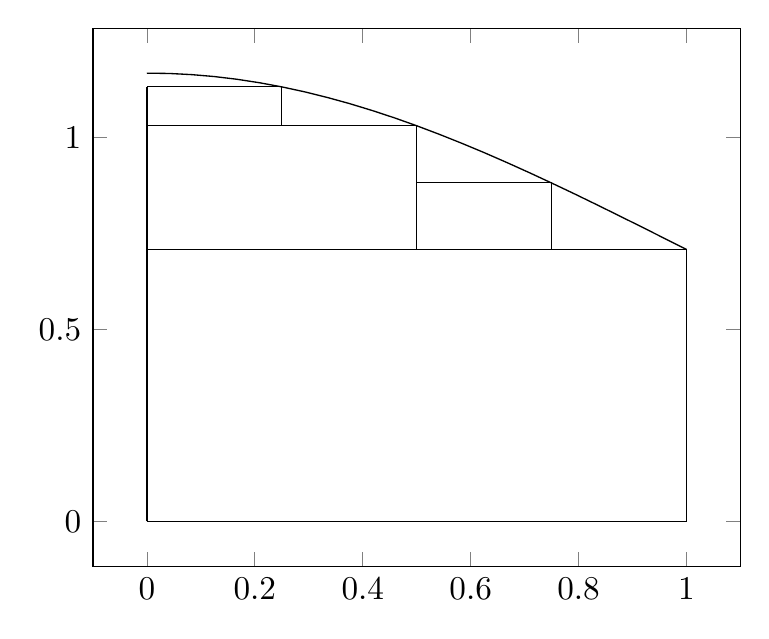
\begin{tikzpicture}[scale=1.2]
\begin{axis}
\addplot[draw=none] coordinates {(0,0)};
\addplot[domain=0:1] {e^(-x^2/2)/0.85624};
\draw (axis cs: 0, 0) -- (axis cs: 1, 0);
\draw (axis cs: 0, 0) -- (axis cs: 0, 0.7088752307384394);
\draw (axis cs: 1, 0) -- (axis cs: 1, 0.7088752307384394);
\draw (axis cs: 0, 0.7088752307384394) -- (axis cs: 1, 0.7088752307384394);
\draw (axis cs: 0, 0.7088752307384394) -- (axis cs: 0, 1.0314073738483691);
\draw (axis cs: 1/2, 0.7088752307384394) -- (axis cs: 1/2, 1.0314073738483691);
\draw (axis cs: 0, 1.0314073738483691) -- (axis cs: 1/2, 1.0314073738483691);
\draw (axis cs: 1/2, 0.7088752307384394) -- (axis cs: 1/2, 0.7088752311585824);
\draw (axis cs: 1, 0.7088752307384394) -- (axis cs: 1, 0.7088752311585824);
\draw (axis cs: 1/2, 0.7088752311585824) -- (axis cs: 1, 0.7088752311585824);
\draw (axis cs: 0, 1.0314073738483691) -- (axis cs: 0, 1.132779392052711);
\draw (axis cs: 1/4, 1.0314073738483691) -- (axis cs: 1/4, 1.132779392052711);
\draw (axis cs: 0, 1.132779392052711) -- (axis cs: 1/4, 1.132779392052711);
\draw (axis cs: 1/4, 1.0314073738483691) -- (axis cs: 1/4, 1.0314073740037737);
\draw (axis cs: 1/2, 1.0314073738483691) -- (axis cs: 1/2, 1.0314073740037737);
\draw (axis cs: 1/4, 1.0314073740037737) -- (axis cs: 1/2, 1.0314073740037737);
\draw (axis cs: 1/2, 0.7088752311585824) -- (axis cs: 1/2, 0.8822094784609293);
\draw (axis cs: 3/4, 0.7088752311585824) -- (axis cs: 3/4, 0.8822094784609293);
\draw (axis cs: 1/2, 0.8822094784609293) -- (axis cs: 3/4, 0.8822094784609293);
\draw (axis cs: 3/4, 0.7088752311585824) -- (axis cs: 3/4, 0.7088752308298532);
\draw (axis cs: 1, 0.7088752311585824) -- (axis cs: 1, 0.7088752308298532);
\draw (axis cs: 3/4, 0.7088752308298532) -- (axis cs: 1, 0.7088752308298532);
\end{axis}
\end{tikzpicture}
	\caption{The normal distribution on the interval $[0,1]$ divided up according to which sections produce distinct prefixes (prefixes up to length 2 have been plotted)}
	\label{fig:normal_bin_cover_2}\vspace{2em}
	
	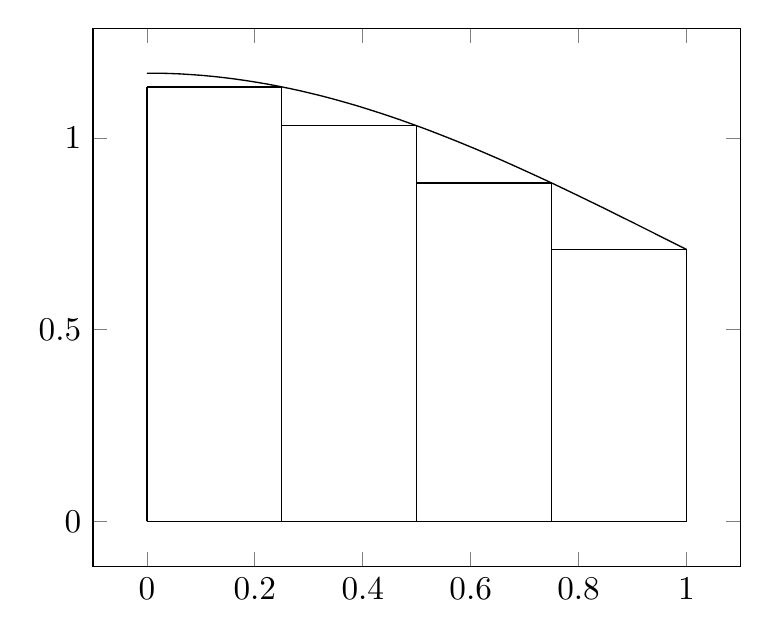
\begin{tikzpicture}[scale=1.2]
\begin{axis}
\addplot[draw=none] coordinates {(0,0)};
\addplot[domain=0:1,samples=50] {e^(-x^2/2)/0.855624};
\draw (axis cs: 0, 0) -- (axis cs: 1, 0);
\draw (axis cs: 0, 0) -- (axis cs: 0, 0.7088752307384394);
\draw (axis cs: 1, 0) -- (axis cs: 1, 0.7088752307384394);
\draw (axis cs: 0, 0) -- (axis cs: 0, 1.0314073738483691);
\draw (axis cs: 1/2, 0) -- (axis cs: 1/2, 1.0314073738483691);
\draw (axis cs: 1/2, 0) -- (axis cs: 1/2, 0.7088752311585824);
\draw (axis cs: 1, 0) -- (axis cs: 1, 0.7088752311585824);
\draw (axis cs: 0, 0) -- (axis cs: 0, 1.132779392052711);
\draw (axis cs: 1/4, 0) -- (axis cs: 1/4, 1.132779392052711);
\draw (axis cs: 0, 1.132779392052711) -- (axis cs: 1/4, 1.132779392052711);
\draw (axis cs: 1/4, 0) -- (axis cs: 1/4, 1.0314073740037737);
\draw (axis cs: 1/2, 0) -- (axis cs: 1/2, 1.0314073740037737);
\draw (axis cs: 1/4, 1.0314073740037737) -- (axis cs: 1/2, 1.0314073740037737);
\draw (axis cs: 1/2, 0) -- (axis cs: 1/2, 0.8822094784609293);
\draw (axis cs: 3/4, 0) -- (axis cs: 3/4, 0.8822094784609293);
\draw (axis cs: 1/2, 0.8822094784609293) -- (axis cs: 3/4, 0.8822094784609293);
\draw (axis cs: 3/4, 0) -- (axis cs: 3/4, 0.7088752308298532);
\draw (axis cs: 1, 0) -- (axis cs: 1, 0.7088752308298532);
\draw (axis cs: 3/4, 0.7088752308298532) -- (axis cs: 1, 0.7088752308298532);
\end{axis}
\end{tikzpicture}
	\caption{This figure is identical to figure 26 except that the thinnest rectangles have been vertically extended}
	\label{fig:normal_bin_cover_riemann}
\end{figure}

So we can estimate the probability that a prefix has length $n$ or less by simply estimating this lower Riemann sum. In particular, we'll do so by finding an upper bound for $\pr{}{\#P>n}$, which is equivalent to the error of the lower Riemann sum.

Let $L_n$ be the lower Riemann sum with the aforementioned partition. And let $m_k$ and $M_k$ be the min and max respectively of $f$ on the interval $[k2^{-n}, (k+1)2^{-n}]$. Then $L_n$ consists of terms that are each of the form
\[
\underbrace{2^{-n}}_{\text{width}} \cdot \underbrace{m_k}_{\text{height}}\,.
\]
On the other hand, the actual area under the curve on such an interval is at most
\[
2^{-n} \cdot M_k\,.
\]
Thus the error on each interval is at most $2^{-n}(M_k-m_k)$. Using the fact that $f$ is $K$-Lipschitz we then get
\[
2^{-n}(M_k-m_k)\leq 2^{-2n}K
\]
as an upper bound on each interval. Thus, the total error is bounded as follows:
\[
\int_0^1f(x)\,dx - L_n \leq 2^n\cdot 2^{-2n}K = 2^{-n}K\,.
\]
In other words $\pr{}{\#R>n}\leq2^{-n}K$. Hence $\pr{}{\#R\leq n}>1-2^{-n}K$.
\end{proof}

Also note that all our inequalities become equalities in the case where $f$ is a straight line. The bound on expected values is now essentially just a corollary.

\begin{proposition}
	Using the previous definitions and assumptions we have for the expected unpadded prefix length 
	\[
	\ev{}{\#R} \leq K
	\]
\end{proposition}
\begin{proof}
The proof is straightforward:
\[
\begin{split}
	\ev{}{\#R} & =\sum_{n=0}^\infty n\,\pr{}{\#R=n}\\
			 & =\sum_{n=1}^\infty n\left(\pr{}{\#R\geq n} - \pr{}{\#R\geq n+1}\right)\\
			 & =\sum_{n=1}^\infty \pr{}{\#R\geq n}\\
			 & \leq\sum_{n=1}^\infty 2^{-n}K\\
			 & = K\,.
\end{split}
\]
\end{proof}

Finally, we can apply this to a distribution with unbounded support.

\begin{proposition}
	Using the previous definitions and assumptions, but where $f$ has arbitrary support we have
	\[
	\ev{}{\#R}\leq\sum_{i\in\mathbb{Z}} K_i
	\]
	where $K_i$ is the Lipschitz constant of $f$ corresponding to the interval $[i,i+1]$.
\end{proposition}
\begin{proof}
We'll use the fact that the Lipschitz constant for $f$ conditioned on the interval $[i,i+1]$ is the same as the Lipschitz constant of $f$ itself on that interval, but normalized by dividing it by $\pr{}{R\in[i,i+1]})$.

\[
\begin{split}
	\ev{}{\#R} & =\sum_{i\in\mathbb{Z}} \ev{}{\#R|R\in[i,i+1]}\cdot\pr{}{R\in[i,i+1]})\\
			   & \leq\sum_{i\in\mathbb{Z}} \frac{K_i}{\pr{}{R\in[i,i+1]})}\cdot\pr{}{R\in[i,i+1]})\\
			   & = \sum_{i\in\mathbb{Z}} K_i
\end{split}
\]
\end{proof}

The infinite sum $\sum_{i\in\mathbb{Z}} K_i$ may look intimidating. But in all but the most pathological cases this will be a quite manageable finite value. For example, we can bound the sum using the absolute values of the first and second derivatives of $f$.

\begin{lemma}
	Given a differentiable function $f : \mathbb{R} \rightarrow \mathbb{R}$ we have
	\[
	\sup_{x\in[a,b]}|f(x)|\leq\int_a^b\frac{|f(x)|}{b-a}+|f'(x)|\,dx
	\]
	 for any $a\leq b$ where $a,b\in\mathbb{R}$.
\end{lemma}
\begin{proof}
Because $f$ is differentiable, it is also continuous. So there exists an $x_1$ such that
\[
f(x_1)=\sup_{x\in[a,b]}|f(x)|\,. 
\]
Furthermore, by the mean value theorem, there exists an $x_2\in[a,b]$ such that
\[
f(x_2)=\frac{1}{b-a}\int_a^b f(x)\,dx\,.
\]
Therefore
\[
\begin{split}
\sup_{x\in[a,b]}|f(x)|-\left|\frac{1}{b-a}\int_a^b f(x)\,dx\right|
& = |f(x_1)|-|f(x_2)|\\
& \leq |f(x_1)-f(x_2)|\\
& = \left|\int_{x_2}^{x_1}f'(x)\,dx\right|\\
& \leq \int_{x_2}^{x_1}|f'(x)|\,dx\\
& \leq \int_{a}^{b}|f'(x)|\,dx\\
\end{split}
\]
which yields
\[
\sup_{x\in[a,b]}|f(x)| \leq \left|\frac{1}{b-a}\int_a^b f(x)\,dx\right|+\int_{a}^{b}|f'(x)|\,dx\leq\int_a^b\frac{|f(x)|}{b-a}+|f'(x)|\,dx\,.
\]
\end{proof}

This lemma is immediately applicable to expected prefix lengths.

\begin{proposition}
	Using the previous definitions and assumptions, if $f$ is twice differentiable, we have
	\[
	\ev{}{\#R}\leq\sum_{i\in\mathbb{Z}} K_i\leq \int_\mathbb{R}|f'(x)|+|f''(x)|\,dx
	\]
\end{proposition}
\begin{proof}
For a differentiable function $f$ the Lipschitz constant $K_i$ is nothing but $\sup_{x\in[i,i+1]}|f'(x)|$. So we can simply apply the previously established bound to each $K_i$ and sum the results.
\end{proof}

Because $f$ integrates to 1, the only way this upper bound could fail to be finite is if $f$ oscillates with exceedingly vanishing amplitude -- aberrant to say the least.

Let's conclude this section by taking the standard normal distribution as an example. First, the sum of the $K_i$: Because the normal distribution is symmetric we can just sum over the positive intervals and double the result. For the first interval $[0,1]$ the maximum slope in absolute value is attained at the right-hand side. For all further intervals it is attained at the left-hand side. Therefore the expected prefix length is bounded by
\[
2\left(|\varphi'(1)|+\sum_{i=1}^\infty |\varphi'(i)|\right) \approx 1.2115\,.
\]
Using the integrals as an upper bound instead produces
\[
\sqrt{\frac{2}{\pi}}+2\,\sqrt{\frac{2}{e\cdot\pi}}\approx 1.7658\,.
\]

Similar considerations for both the exponential and the sinusoidal distribution allow us to give the following summary.
\begin{center}
\begin{tabular}{l | c | c | c}
& numerical estimate & $\sum_i K_i$ & $\int |f'| + |f''|\,dx$\\
\hline
standard normal & 0.1846 & 1.2115 & 1.7658\\
exponential & 0.5626 & 1.5820 & 2\\
sinusoidal & 3.4979 & 12.5664 & 108.5310\\
\end{tabular}
\end{center}
These examples showcase both scenarios where the upper bounds are reasonably tight and where they are not.





\section{The Uniformity Of Trailing Digits}

We've now seen that under relatively minor assumptions the prefixes of continuous distributions are quite short. This also means that the trailing digits of continuous distributions rapidly converge to the uniform distribution. We now make this statement more exact. The following discussion won't rely on insights based on prefixes and is instead essentially a generalization of an argument that is suggested by Arif Zaman in \cite{Zaman}.

\begin{theorem}
	Let $X$ be a random variable that is distributed continuously according to a Riemann integrable density function $f$. Then the trailing digits $n$ places beyond the decimal point, when interpreted as a real number in the interval $[0,1]$, converge in distribution to the standard uniform distribution as $n\rightarrow\infty$.
\end{theorem}
\begin{proof}
We begin by denoting the fractional part of $X$ as $\{X\}$. Then the density of $\{X\}$ is given by
\[
\tilde{f}(x) =
\begin{cases}
\sum_{i\in\mathbb{Z}}f(i+x) & 0 < x \leq 1\\
0 & \text{otherwise}
\end{cases}
\]
The case $0<x\leq1$ follows from the fact that, if we denote the corresponding cumulative distribution functions $F$ and $\tilde{F}$, then clearly for $0<x\leq1$ we have
\[
\tilde{F}(x) = \sum_{i\in\mathbb{Z}}F(i+x)-F(i)\,.
\]
We're just summing up all the probabilities corresponding to intervals $[i,i+x]$ where the fractional part is less than $x$. Then differentiate both sides with respect to $x$.
\[
\begin{split}
\tilde{f}(x) & =\frac{d}{dx}\sum_{i\in\mathbb{Z}}F(i+x)-F(i)\\
			 & =\frac{d}{dx}\sum_{i\in\mathbb{Z}}\int_0^x f(i+x)\,dx\\
			 & =\frac{d}{dx}\int_0^x\sum_{i\in\mathbb{Z}}f(i+x)\,dx\qquad\text{by Fubini's theorem}\\
			 & =\sum_{i\in\mathbb{Z}}f(i+x)\,dx
\end{split}
\]

Now that we know the density of $\{X\}$, the density for digits that are trailing $n$ places beyond the decimal point is close at hand. If we continue expressing our numbers in binary it'll be the density of the random variable $\{2^nX\}$. After all, multiplying by $2^n$ just shifts all the bits $n$ places to the left.

The density $f_{2^n}$ of $2^nX$ is given by transforming the density for $X$ as
\[
f_{2^n}(x) = \frac{1}{2^n}f\left(\frac{x}{2^n}\right)\,.
\]
Thus, just as before, we get the following density for $\{2^nX\}$:
\[
\tilde{f}_{2^n}(x)=
\begin{cases}
\sum_{i\in\mathbb{Z}}\frac{1}{2^n}f\left(\frac{i+x}{2^n}\right) & 0<x\leq 1\\
0 & \text{otherwise}
\end{cases}
\]
Notice that this is really just a Riemann sum again. For any fixed $x$ we're evaluating $f$ at distances $2^{-n}$ apart and multiplying the result by the width of the corresponding interval. Since $f$ integrates to 1, we get
\[
\lim_{n\rightarrow\infty}\tilde{f}_{2^n}(x) = 
\begin{cases}
1 & 0<x\leq 1\\
0 & \text{otherwise}
\end{cases}
\]
which is exactly the density of the standard uniform distribution.
\end{proof}

Further, we can see that this convergence tends to be extremely rapid. We can measure this, for instance, in terms of the $L_1$-distance between $f_{2^n}$ and the standard uniform density. The argument follows the same lines as the previous section.

\begin{proposition}
	Given a density function $f$, if $f$ is $K$-Lipschitz and has support $[i,i+1]$, $i\in\mathbb{Z}$, then
	\[
	\int_\mathbb{R} \left|\underset{[0,1]}{\mathbf{1}}(x)-\tilde{f}_{2^n}(x)\right|\,dx\leq2^{-n}K
	\]
	where $\mathbf{1}_{[0,1]}$ is the indicator function for the interval $[0,1]$ and $\tilde{f}_{2^n}$ is the density of the trailing digits beyond the $n$th bit.
\end{proposition}
\begin{proof}
$\mathbf{1}_{[0,1]}$ and $\tilde{f}_{2^n}$ are both equal everywhere outside the interval $[0,1]$. On the interval $[0,1]$ on the other hand, $\mathbf{1}_{[0,1]}=1$ and $\tilde{f}_{2^n}(x)$ is a Riemann sum for any fixed $x$. Since it is the Riemann sum for $f$ which integrates to 1, $\left|1-\tilde{f}_{2^n}(x)\right|$ is really just the error of the Riemann sum. And we've already seen in the proof of proposition \ref{a} how we can bound this error above by $2^{-n}K$
\end{proof}

This leads straight to:

\begin{proposition}
	Using the previous definitions and assumptions, if $f$ has arbitrary support, we have
	\[
	\int_\mathbb{R} \left|\underset{[0,1]}{\mathbf{1}}(x)-\tilde{f}_{2^n}(x)\right|\,dx\leq2^{-n}\sum_{i\in\mathbb{Z}}K_i
	\]
	where $K_i$ is the Lipschitz constant of $f$ corresponding to the interval $[i,i+1]$.
\end{proposition}
\begin{proof}
For densities with arbitrary support we get an error of at most $2^{-n}K_i$ on every interval of unit length by the previous result. We simply sum these errors over all $i\in\mathbb{Z}$.
\end{proof}

Of course the sum over the $K_i$ is a familiar face from the previous section. So we can immediately also give the upper bound $2^{-n}\int_\mathbb{R}|f'(x)|+|f''(x)|\,dx$, provided that $f$ is twice differentiable.\\

Arif Zaman was brought to the distribution of fractions by examining a wheel of fortune and asking what the distribution of the resting position for the wheel might be. He assumed the circumference of the wheel to be normed to 1 and that the total distance traveled was a normally distributed random variable $X$. Since the wheel effectively removes the integer part of $X$ after each rotation, the resting position will then be $\{X\}$.

Now a wheel of fortune may seem like a rather droll thing to study, but in fact wheels of fortune are all over the place. Take any physical measurement that is performed to high accuracy and look at its bits $n$ places beyond the decimal point. This is nothing other than a wheel of fortune that has been normed to length $2^{-n}$! 



\section{Some Impossibility Results}

Most of this thesis has focused on continuous distributions and their prefixes. We'll now close with two results regarding discrete distributions from a completely different arena -- the theory of computation. 

The fact that we could sample exactly from virtually any discrete distribution might have come as a slight surprise to some. And it raises the question where the limits of the tools we have considered are. In fact, are there \textit{any} discrete distributions which one can \textit{not} sample exactly using exact bisection sampling or similar means? Indeed, there are -- though they are admittedly somewhat esoteric.

To begin with, we'll have to recall the undecidability of the halting problem established by Alan Turing in \cite{Turing}. Because the argument is so disarmingly simple, we'll briefly recount it here.

\begin{theorem}
	There is no algorithm $H$ (alternatively Turing machine or computer program), accepting as inputs the description of another algorithm $A$ and a string $x$, that can within a finite amount of time determine whether $A$, when run on $x$, halts.
\end{theorem}
\begin{proof}
As with all the proofs in this section, we argue by contradiction. Suppose such an algorithm $H$ exists. Then one can easily modify it into a new algorithm $\overline{H}$ that only takes a single argument $A$ defined as 
\[
\overline{H}(A) =
\begin{cases}
\text{enter an infinite loop} & \text{if }H(A,A)=\text{ true}\\
\text{terminate} & \text{if }H(A,A)=\text{ false}
\end{cases}
\]
Because $H(A, x)$ supposedly correctly determines whether $A$ halts on $x$, this is equivalent to
\[
\overline{H}(A) =
\begin{cases}
\text{enter an infinite loop} & \text{if }A(A)\text{ halts}\\
\text{terminate} & \text{if }A(A)\text{ doesn't halt}
\end{cases}
\]
We use "terminate" because it really doesn't matter what $\overline{H}$ outputs in that case. It only matters that $\overline{H}$ halts. Now the question is: Does $\overline{H}(\overline{H})$ halt? There are two options.
\begin{itemize}
	\item $\overline{H}(\overline{H})$ \textbf{halts}: But then by the definition of $\overline{H}$ it doesn't halt. \lightning
	\item $\overline{H}(\overline{H})$ \textbf{doesn't halt}: But then by the definition of $\overline{H}$ it halts. \lightning
\end{itemize}
Either way, we get a contradiction. So we're forced to accept that $H$ can't exist.
\end{proof}

How do we turn this into a discrete distribution from which it is impossible to sample exactly? Like so:

\begin{proposition}
	Let $(A_n)$ be an enumeration of all possible algorithms. And let $(A_{n_k})$, $k$ starting at 1, be a subsequence consisting of all the non-halting algorithms (algorithms that don't halt when given themselves as input).
	
	Then there doesn't exist any randomized algorithm (an algorithm that has access to random bits during its computation) that can sample exactly from the distribution with probability mass function 
	\[
	P(i) = 
	\begin{cases}
	2^{-k} & \text{if $i=n_k$ for some $k$}\\
	0 & \text{otherwise}
	\end{cases}
	\]
	where $i\in\mathbb{N}$.
\end{proposition}
In other words, we've just placed some discrete distribution with infinite support, the geometric distribution with $p = 1/2$ to be exact, on the set of non-halting algorithms. 
\begin{proof}
It is an elementary result in the theory of computation that the set of non-halting algorithms can't be enumerated (in any order, possibly with repetitions). Suppose we could. Then we could solve the halting problem for any algorithm $A$ by doing the following in alternating fashion.
\begin{itemize}
	\item Run $A$ for a couple steps and see if it has halted yet. 
	\item List out a few non-halting algorithms and see if $A$ shows up.
\end{itemize}
This process would sooner or later determine whether $A$ halts. But we've already seen that this cannot be done. Now it is definitely possible to run $A$ for a few steps at a time. So it must be that it is impossible to enumerate the non-halting algorithms.

Since we can't even list the non-halting algorithms it will come as no surprise that we can't sample from them either. Usually these impossibility results proceed via a reduction. Just as in the previous paragraph, one demonstrates that, if it was possible to perform some task $T$, then one could indirectly solve the halting problem. Hence $T$ is impossible. But how do we use a random process to solve a problem such as the halting problem which demands a definite yes-or-no answer?

The solution is to use a strategy known as \textit{derandomization}. This strategy usually entails taking a fast randomized algorithm and significantly shrinking the sample space of that algorithm. It may then become computationally feasible to exhaustively check through the entire sample space, yielding a deterministic algorithm that is now guaranteed to produce the correct result.

We can reuse this idea of exhaustive checking to derandomize the supposed randomized algorithm that can sample from the indices of non-halting Turing machines. If we call this algorithm $N$, then one can turn this algorithm into a determinstic algorithm by making the random bits it has access to an input $r$ of $N$. We then repeatedly call $N$ on all possible finite sequences, one after the other.

Because the indices of halting algorithms are sampled with probability 0, these will never appear as the output of $N$. On the other hand, for any given non-halting algorithm $A_{n_k}$ there is a non-zero probability of $n_k$ being produced by $N$. In other words, there must exist an input $r_k$ such that $N(r_k) = n_k$. Sooner or later we'll reach $r_k$, thus listing out $n_k$. And it is easy to use that to list out $A_{n_k}$ itself. So we have found a procedure that enumerates all non-halting algorithms, which is impossible. \lightning
\end{proof}

The second impossibility result concerns exact Bernoulli sampling. All the way back in the introduction there was the innocuous remark that Bernoulli sampling can be performed for any computable number, which is a number whose digits can be listed out by some algorithm. It is easy to show that there are numbers that aren't computable. After all, there are only countably many algorithms, yet uncountably many real numbers. So there must be quite a few real numbers that won't be listed out by any algorithm. Now one might ask if there's perhaps an even more remarkable trick which can't just perform exact Bernoulli sampling for computable numbers, but also for a few uncomputable ones.

\begin{proposition}
	There exists no randomized algorithm that can sample exactly from the distribution with probability mass function
	\[
	P(i)=
	\begin{cases}
	p & \text{i=0}\\
	1-p & \text{i=1}\\

	\end{cases}
	\]
	where $i\in\{0,1\}$ and $p$ is not a computable number.
\end{proposition}
\begin{proof}
Suppose this was possible using some algorithm $N$ using random bits $r$ as its only input. We will again derandomize $N$ -- looping through all possible values of $r$ -- to produce an algorithm that can exactly list out the digits of $p$.

When iterating through the possible values of $r$, there will be many for which $N$ hasn't terminated yet. We ignore those. But suppose we reach a value $r_k$ so that $N(r_k)=0$. We will then also know that $N$ outputs 0 for any string of bits that are a continuation of $r_k$. So if $\#r_k$ is the number of bits in $r_k$, we can conclude that there is at least a $2^{-\#r_k}$ chance that $N$ will output 0. We can add this probability to a tally we're keeping for the probability of sampling 0.

If we do the same thing for the output 1, then we'll be able to track two partial sums that are converging to $p$ both from above and below. If they didn't converge, then either $N$ wouldn't be sampling with the correct probabilities or there would exist a non-zero probability that $N$ never terminates. The gap between these partial sums will eventually close far enough to determine every digit of $p$, one after the other. But that's impossible. \lightning
\end{proof}





\begin{thebibliography}{9}
\bibitem{Knuth-Yao}
Donald Knuth \& Andrew Yao, 1976, The complexity of nonuniform random number generation, Algorithms and
Complexity: New Directions and Recent Results, pages 357–428

\bibitem{Karney}
Charles F. F. Karney, 2016, Sampling exactly from the normal distribution, ACM Transactions on Mathematical Software, Volume 42, Issue 1

\bibitem{Zaman}
Arif Zaman, 2004, The Density of the Fractional Part of a Normal Distribution

\bibitem{Turing}
Alan Turing, 1937, On Computable Numbers, with an Application to the Entscheidungsproblem, Proceedings of the London Mathematical Society
\end{thebibliography}

\section{Appendix}

The following is a listing of the code that was used to compute the probabilities of various prefixes. It is written in Clojure, a descendant of Lisp.

\begin{lstlisting}[breaklines=true, basicstyle=\small]
(ns exact-sampling.plot
  (:require [clojure.math.numeric-tower :refer [expt]]
            [clojure.string :as str])
  (:import (org.apache.commons.math.optimization MultiStartUnivariateRealOptimizer GoalType)
           (org.apache.commons.math.optimization.univariate BrentOptimizer)
           (org.apache.commons.math.random JDKRandomGenerator)
           (org.apache.commons.math.analysis UnivariateRealFunction)))

(def minimize
  "Finds the minimum of a function f on the interval [a,b]."
  (memoize
    (fn [f a b]
      (-> (MultiStartUnivariateRealOptimizer. (BrentOptimizer.) 100 (JDKRandomGenerator.))
          (.optimize (reify UnivariateRealFunction (value [_ x] (f x))) GoalType/MINIMIZE a b)
          (f)))))

(defn prefix-to-number [[base digits]]
  "Given a base and a sequence of digits in that base, returns the corresponding number."
  (->> digits
       (map-indexed #(* (expt base (- (inc %1))) %2))
       (reduce +)))

(defn prefix-to-interval-length [[base digits]]
  "Given a base and a sequence of digits in that base, returns the width of the interval
  corresponding to all numbers in that base beginning with those digits."
  (expt base (- (count digits))))

(defn prefix-to-interval [[base digits]]
  "Given a base and a sequence of digits in that base, returns a tuple [a,b] denoting the interval
   corresponding to all numbers in that base beginning with those digits."
  (let [a (prefix-to-number [base digits])]
    [a (+ a (prefix-to-interval-length [base digits]))]))

(defn prefix-to-probability [f [base digits]]
  "Given a probability density function f, a base, and a sequence of digits, returns the probability
  that an unpadded prefix in the given base with the given digits will be selected."
  (if (empty? digits)
    (minimize f 0 1)
    (let [current-min (apply minimize f (prefix-to-interval [base digits]))
          previous-min (apply minimize f (prefix-to-interval [base (butlast digits)]))]
      (* (- current-min previous-min) (prefix-to-interval-length [base digits])))))

(defn leading-digits [digits]
  "Given a sequence of digits, returns a sequence of prefix sequences ending with the empty sequence.
  E.g. 101 yields (10, 1, [])."
  (concat (take-while some? (iterate butlast (butlast digits))) [[]]))

(defn padded-prefix-to-probability [f [base digits]]
  "Given a probability density function f, a base, and a sequence of digits, returns the probability
  that a padded prefix in the given base with the given digits will be selected."
  (if (or (empty? digits) (zero? (last digits)))
    0
    (->> (leading-digits digits)
         (take-while #(or (empty? %) (zero? (last %))))
         (map-indexed #(* (expt base (- (inc %1))) (prefix-to-probability f [base %2])))
         (reduce +)
         (+ (prefix-to-probability f [base digits])))))

(defn digits-up-to-length-n [base n]
  "Returns a sequence of all sequences of digits up to length n in the given base."
  (->> (iterate #(mapcat (fn [digits] (map (partial conj digits) (range base))) %) [[]])
       (take (inc n))
       (apply concat)))

(defn probability-map-0-1 [f base n]
  "Takes a probability density function f with support [0,1], a base, and a maximum prefix length n.
  Returns a map from the padded prefixes (represented as doubles) to their corresponding probabilities."
  (->> (digits-up-to-length-n base n)
       (map #(vector (prefix-to-number [base %]) (padded-prefix-to-probability f [base %])))
       (filter #(pos? (second %)))
       (into (sorted-map))))

(defn probability-map [f base n a b]
  "Takes a probability density function f with arbitrary support, a base, and a maximum prefix length n.
  Returns a map from the padded prefixes (represented as doubles) to their corresponding probabilities."
  (->> (range a b)
       (mapcat #(->> (probability-map-0-1 (comp f (partial + %)) base n)
                     (map (fn [[x p]] [(+ x %) p]))
                     (into (sorted-map))))))
\end{lstlisting}

\end{document}
